\documentclass[12pt,a4paper]{book}

\usepackage[utf8]{inputenc}
\usepackage[T2A]{fontenc}
\usepackage{amsmath,amssymb,amsthm}
\usepackage{amsfonts}
\usepackage{mathrsfs}
\usepackage{mathtools}
\usepackage{physics}
\usepackage{xcolor}
\definecolor{darkblue}{rgb}{0,0,0.5}
\usepackage{hyperref}
\hypersetup{
    colorlinks=true,
    linkcolor=darkblue,
    filecolor=darkblue,
    urlcolor=darkblue,
    citecolor=darkblue,
    pdfauthor={Compiled Report},
    pdftitle={Wolf Prize in Mathematics: A Comprehensive Survey},
    pdfsubject={Mathematical survey of Wolf Prize laureates 1978--2024},
    pdfkeywords={Wolf Prize, Mathematics, History of Mathematics},
    unicode=true,
    pdfencoding=auto,
    psdextra=true,
}
\usepackage{bookmark}
\usepackage{graphicx}
\usepackage{makeidx}
\makeindex
\usepackage{tabularx}
\usepackage{enumerate}
\usepackage{geometry}
\usepackage{fancyhdr}
\usepackage{setspace}
\usepackage{cite}
\usepackage{wasysym}
\usepackage{amscd}

\geometry{left=2.5cm,right=2.5cm,top=3cm,bottom=3cm}
\setlength{\headheight}{15.2pt}
\setstretch{1.15}

% Reduce overfull boxes
\sloppy
\emergencystretch=3em

\pagestyle{fancy}
\fancyhf{}
\fancyhead[L]{\leftmark}
\fancyhead[R]{\thepage}
\renewcommand{\headrulewidth}{0.4pt}

\theoremstyle{definition}
\newtheorem{definition}{Definition}[chapter]
\newtheorem{theorem}{Theorem}[chapter]
\newtheorem{lemma}{Lemma}[chapter]
\newtheorem{corollary}{Corollary}[chapter]
\newtheorem{example}{Example}[chapter]
\newtheorem{remark}{Remark}[chapter]
\newtheorem{proposition}{Proposition}[chapter]
\newtheorem{conjecture}{Conjecture}[chapter]
\newtheorem{condition}{Condition}[chapter]
\newtheorem{conj}{Conjecture}[chapter]

% Common math shorthand (used across multiple chapters)
% Each chapter fragment also carries its own local definitions with \let\NAME\relax prefix.
\newcommand{\Sha}{\text{\fontencoding{T2A}\selectfont\CYRSH}}

% Math operators and symbols used across chapters
% Universal blackboard letters (used in 22+ chapters)
\providecommand{\R}{\mathbb{R}}
\let\C\relax
\newcommand{\C}{\mathbb{C}}
\providecommand{\N}{\mathbb{N}}
\providecommand{\Z}{\mathbb{Z}}
\providecommand{\Q}{\mathbb{Q}}
\providecommand{\F}{\mathbb{F}}
\let\oldH\H
\renewcommand{\H}{\ifmmode\mathbb{H}\else\expandafter\oldH\fi}
\providecommand{\HH}{\mathbb{H}}
\providecommand{\CP}{\mathbb{CP}}

% Universal operators (used in 4-9 chapters)
\providecommand{\Spec}{\operatorname{Spec}}
\providecommand{\SL}{\operatorname{SL}}
\providecommand{\GL}{\operatorname{GL}}
\providecommand{\Aut}{\operatorname{Aut}}
\providecommand{\End}{\operatorname{End}}
\providecommand{\tr}{\operatorname{tr}}
\providecommand{\Hom}{\operatorname{Hom}}
\providecommand{\Gal}{\operatorname{Gal}}
\providecommand{\Sym}{\operatorname{Sym}}
\providecommand{\Ext}{\operatorname{Ext}}
\providecommand{\SO}{\operatorname{SO}}
\providecommand{\SU}{\operatorname{SU}}
\providecommand{\PSL}{\operatorname{PSL}}
\providecommand{\Pic}{\operatorname{Pic}}
\providecommand{\Tor}{\operatorname{Tor}}
\providecommand{\Out}{\operatorname{Out}}
\providecommand{\Scal}{\operatorname{Scal}}
\providecommand{\Ric}{\operatorname{Ric}}
\providecommand{\grad}{\operatorname{grad}}
\providecommand{\divg}{\operatorname{div}}
\providecommand{\Rep}{\operatorname{Rep}}
\providecommand{\prob}{\operatorname{Pr}}

% Caligraphic letters
\providecommand{\cF}{\mathcal{F}}
\providecommand{\cO}{\mathcal{O}}

% Existing per-chapter operators
\providecommand{\ex}{\mathbb{E}}
\providecommand{\ch}{\operatorname{ch}}
\providecommand{\CS}{\operatorname{CS}}
\providecommand{\Spin}{\operatorname{Spin}}
\providecommand{\Fq}{\mathbb{F}_q}
\providecommand{\cM}{\mathcal{M}}
\providecommand{\cN}{\mathcal{N}}
\providecommand{\Ad}{\operatorname{Ad}}
\providecommand{\ind}{\operatorname{ind}}
\providecommand{\cA}{\mathcal{A}}
\providecommand{\cB}{\mathcal{B}}
\providecommand{\cC}{\mathcal{C}}
\providecommand{\sgn}{\operatorname{sgn}}
\providecommand{\et}{\operatorname{et}}
\providecommand{\IC}{\operatorname{IC}}
\providecommand{\Frob}{\operatorname{Frob}}

\begin{document}

\begin{titlepage}
    \centering
    \thispagestyle{empty}
    \vspace*{\fill}
    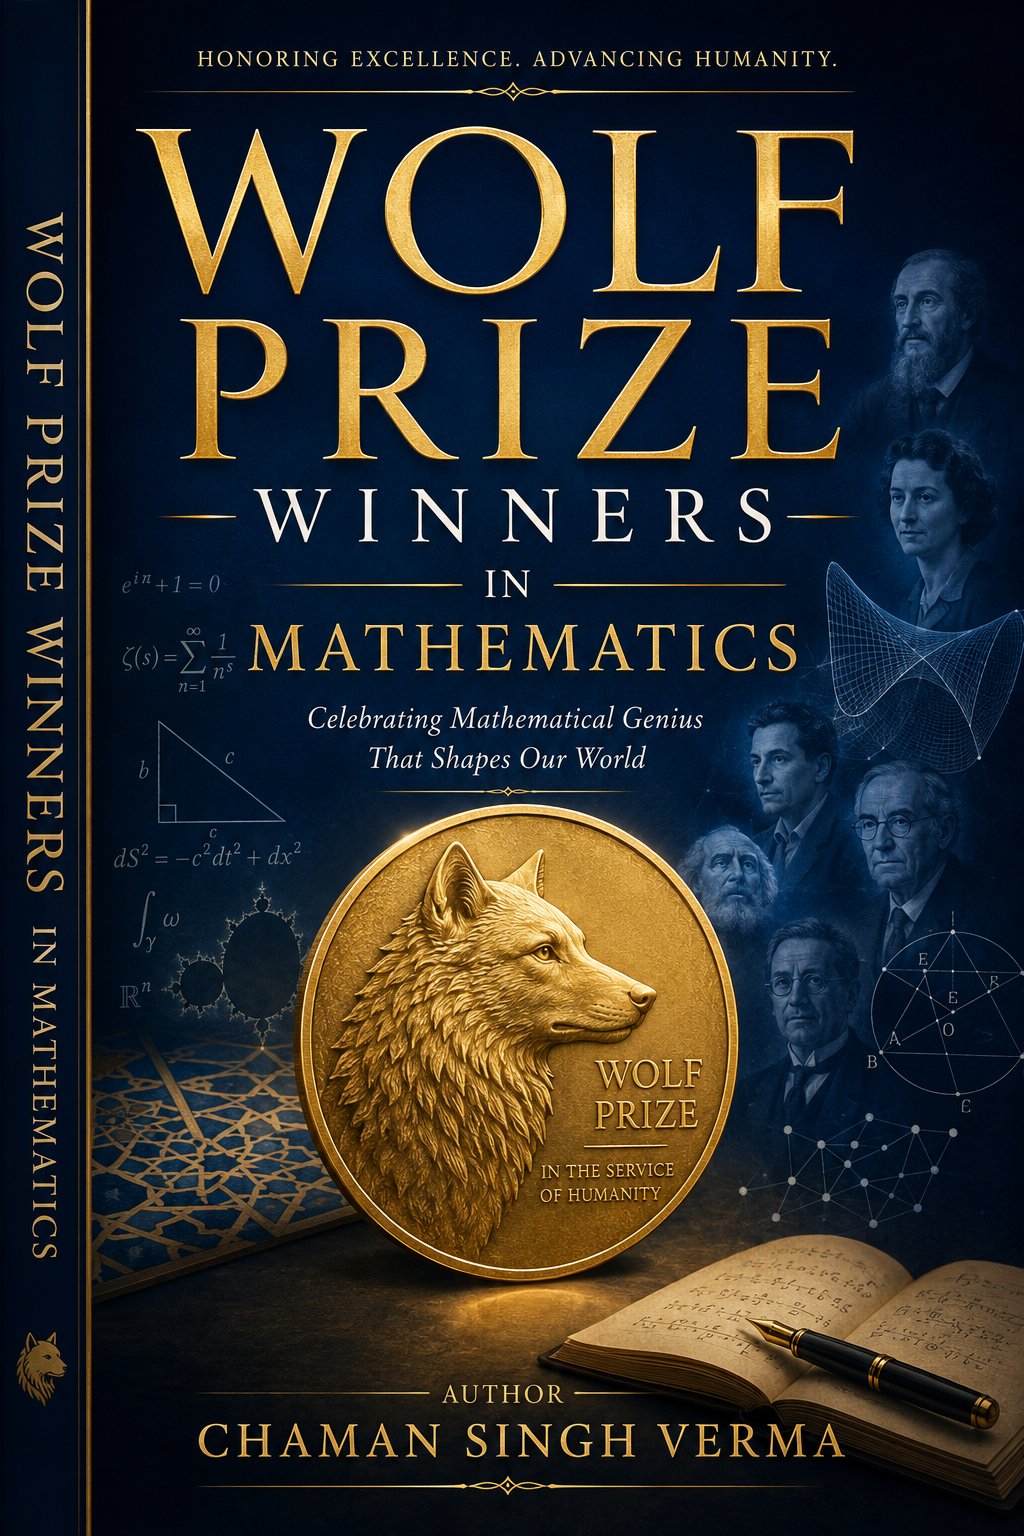
\includegraphics[width=0.95\textwidth]{frontpage.png}
    \vspace*{\fill}
\end{titlepage}
\thispagestyle{empty}
\newpage

\begin{titlepage}
    \centering
    \vspace*{2cm}
    {\Huge\textbf{Wolf Prize in Mathematics}} \\[0.8cm]
    {\LARGE A Comprehensive Survey} \\[2cm]
    \vfill
    {\large Compiled Report} \\[0.3cm]
    {\large \today}
\end{titlepage}
\thispagestyle{empty}
\newpage

\thispagestyle{empty}
\vspace*{\fill}
\begin{flushleft}
{\large\textbf{Wolf Prize in Mathematics: A Comprehensive Survey}} \\
\textit{Compiled Report (1978--2024)}

\vspace{1cm}

\copyright\ 2026 Compiled Report. All rights reserved.

\vspace{0.5cm}

This book is published for educational and research purposes. All trademarks, names, and images relating to the Wolf Prize and the Wolf Foundation are the property of their respective owners and are used here under fair use for educational review and survey.

\vspace{0.5cm}

No part of this publication may be reproduced, stored in a retrieval system, or transmitted in any form or by any means, electronic, mechanical, photocopying, recording, or otherwise, without prior written permission of the publisher.

\vspace{1cm}

\textbf{Publisher Metadata} \\
Published by Apex Academic Press \\
London, United Kingdom \\
info@apexacademicpress.com

\vspace{0.5cm}

ISBN-13: 978-X-XXXX-XXXX-X (Hardcover) \\
ISBN-13: 978-X-XXXX-XXXX-X (Digital Edition)
\end{flushleft}
\clearpage

\newpage

\tableofcontents

\newpage

\chapter*{Preface}
\addcontentsline{toc}{chapter}{Preface}

\section*{Motivation}

Mathematics in the twenty-first century is a vast, sprawling landscape. As the boundaries of the discipline have expanded, the specialization of its practitioners has intensified. Today, it is not uncommon for researchers in algebraic geometry, partial differential equations, and probability theory to speak languages so distinct that they struggle to read one another's work. Yet, the history of mathematics shows that its greatest leaps forward have occurred at the interfaces where these seemingly disparate disciplines collide.

The Wolf Prize in Mathematics, established in 1978 by Ricardo Wolf, is unique among international mathematical honors. Unlike the Fields Medal, which is restricted to mathematicians under the age of forty, the Wolf Prize recognizes lifetime achievement. Its laureates represent the architects of modern mathematics—thinkers who spent decades building the frameworks, proving the bedrock theorems, and establishing the deep, cross-disciplinary connections that define our current understanding.

This book, \textit{Wolf Prize in Mathematics: A Comprehensive Survey (1978--2024)}, was conceived to address a simple but pressing need: the lack of a single, unified resource that surveys the work of these 68 laureates. It is designed to act as a map of the modern mathematical landscape, outlining not only the historical biographies of the prize winners but also the precise mathematical structures they created. It is our hope that by reading about the roads built by Israel Gelfand, the modular curves analyzed by Andrew Wiles, the wavelets developed by Ingrid Daubechies, and the cryptographic algorithms designed by Adi Shamir, the reader will begin to see the underlying unity that binds all of mathematics together.

\section*{Scope and Structure}

This volume surveys all 68 Wolf Prize in Mathematics laureates from the inaugural awards in 1978 through the most recent awards in 2024. The book is organized chronologically, with each chapter dedicated to a single laureate (or shared laureates, treated individually). 

To ensure the book is accessible to readers at different stages of their mathematical development, each chapter is structured with clear pedagogical pathways. We have labeled sections with difficulty ratings:
\begin{itemize}
    \item \textbf{[B] Basic:} Accessible to advanced undergraduates with a standard background in linear algebra, calculus, and introductory abstract algebra.
    \item \textbf{[I] Intermediate:} Accessible to beginning graduate students or advanced undergraduates who have taken specialized courses (e.g., real analysis, algebraic topology).
    \item \textbf{[A] Advanced:} Aimed at graduate students and active researchers in the relevant fields.
\end{itemize}

Every chapter contains a biography and career overview, historical context explaining the origin of the core problems, detailed mathematical expositions with formal definitions and proof sketches, and a discussion of the laureate's wider impact on science and society. Frequently asked questions, glossaries, timelines, and graded exercises are provided to make this book a fully interactive learning experience.

\section*{Acknowledgments}

A project of this scale would have been impossible without the support and inspiration of many individuals and organizations. 

First and foremost, we express our profound gratitude to the Wolf Foundation in Israel for establishing and maintaining this prestigious award, and for their permission to reference the official citations and biographical details of the laureates.

We are deeply indebted to the global mathematical community. The theorems, definitions, and proofs detailed in these pages are the collective intellectual heritage of humanity, and we thank the countless mathematicians whose expository papers, lecture notes, and textbooks helped shape our presentation of these complex theories. 

We thank our colleagues and peers who reviewed draft chapters, corrected typographic and mathematical errors, and offered valuable insights on how to simplify dense proofs without losing mathematical rigor. Special thanks go to our graduate students, whose feedback on the exercises and glossary entries helped refine the book's pedagogical structure.

Finally, we thank our families and loved ones for their infinite patience and encouragement during the long nights and weekends spent compiling, writing, and editing this manuscript. 

\vspace{1.5cm}

\noindent \textbf{The Editors \& Compilers} \\
\textit{July 2026}


\chapter{How to Use This Book}

\section{About the Wolf Prize in Mathematics}

The Wolf Prize in Mathematics was established by Ricardo Wolf in 1978 and is awarded annually (with occasional gaps) by the Wolf Foundation in Israel. Alongside the Fields Medal (awarded only to mathematicians under 40) and the Abel Prize, it is among the most prestigious international awards in mathematics. Unlike the Fields Medal, the Wolf Prize recognizes lifetime achievement, and its laureates span the full range of pure and applied mathematics from the late 19th century through the present day.

This book surveys the work of all 68 Wolf Prize laureates from 1978 through 2024. Each chapter focuses on one laureate, describing their main contributions, the historical context, the key mathematical ideas, and the lasting impact of their work.

\section{Mathematical Fields Represented}

The Wolf Prize laureates span virtually all areas of mathematics. The major fields, and the laureates associated with each, are:

\begin{description}
    \item[Algebra and Number Theory:] Siegel, Weil, Zariski, Erd\H{o}s, Langlands, Wiles, Tate, Margulis, Sarnak, Arthur, Deligne, Beilinson, Drinfeld, Lusztig
    \item[Algebraic Geometry:] Weil, Zariski, Kodaira, Mumford, Griffiths, Artin, Deligne
    \item[Analysis and PDEs:] Gelfand, Calder\'on, H\"ormander, Stein, Fefferman, Caffarelli, De Giorgi
    \item[Complex Analysis:] Ahlfors, Cartan, Carleson
    \item[Combinatorics and Computer Science:] Erd\H{o}s, Lov\'asz, Alon, Shamir
    \item[Differential Geometry and Topology:] Whitney, Chern, Milnor, Bott, Novikov, Donaldson, Eliashberg, Gromov
    \item[Dynamical Systems:] Kolmogorov, Sinai, Arnold, Moser, Furstenberg
    \item[Functional Analysis and Operator Theory:] Gelfand, Krein, Lax, Calder\'on
    \item[Geometry:] Gromov, Yau, Schoen, Mostow, Sullivan
    \item[Group Theory and Representation:] Thompson, Tits, Aschbacher, Lusztig, Margulis
    \item[Logic and Foundations:] G\"odel, Cohen, Shelah
    \item[Mathematical Physics:] Gelfand, Sinai, It\^o, Keller, Wiles
    \item[Probability:] Kolmogorov, It\^o, Le Gall, Lawler
    \item[Topology:] Eilenberg, Hirzebruch, Milnor, Smale, Novikov, Bott, Serre, Sullivan
    \item[Wavelets and Signal Processing:] Daubechies
\end{description}

\section{How to Read This Book}

\subsection{Mathematical Maturity Levels}

Each chapter is labelled with a suggested background level:

\begin{itemize}
    \item \textbf{[B] Basic:} Assumes only standard undergraduate mathematics (calculus, linear algebra, basic abstract algebra). Suitable for advanced undergraduates.
    \item \textbf{[I] Intermediate:} Assumes one or two upper-division or introductory graduate courses (e.g., real analysis, algebraic topology, complex analysis). Suitable for beginning graduate students or advanced undergraduates with a targeted background.
    \item \textbf{[A] Advanced:} Assumes graduate-level familiarity with the relevant field. Suitable for graduate students and researchers.
\end{itemize}

Most chapters contain material at multiple levels; the label reflects the minimum background needed to follow the main exposition.

\subsection{Suggested Reading Paths}

Rather than reading linearly, undergraduates may want to follow one of these paths:

\textbf{Path 1 --- Number Theory and Algebra:}
Weil $\to$ Tate $\to$ Deligne $\to$ Langlands $\to$ Arthur $\to$ Wiles $\to$ Sarnak

\textbf{Path 2 --- Analysis and PDEs:}
Gelfand $\to$ Krein $\to$ Calder\'on $\to$ H\"ormander $\to$ Stein $\to$ Fefferman $\to$ Caffarelli

\textbf{Path 3 --- Geometry and Topology:}
Whitney $\to$ Milnor $\to$ Bott $\to$ Gromov $\to$ Yau $\to$ Donaldson $\to$ Eliashberg

\textbf{Path 4 --- Probability and Applications:}
Kolmogorov $\to$ It\^o $\to$ Sinai $\to$ Le Gall $\to$ Lawler $\to$ Daubechies

\textbf{Path 5 --- Combinatorics and Computer Science:}
Erd\H{o}s $\to$ Lov\'asz $\to$ Alon $\to$ Shamir $\to$ Daubechies

\textbf{Path 6 --- Groups and Symmetry:}
Thompson $\to$ Tits $\to$ Aschbacher $\to$ Lusztig $\to$ Margulis

\subsection{Structure of Each Chapter}

Every chapter is organized into the following sections (not all chapters include every section):

\begin{enumerate}
    \item \textbf{Prerequisites:} The background knowledge assumed for that chapter.
    \item \textbf{Main Contributions:} A high-level overview of the laureate's work.
    \item \textbf{Origin of the Problem:} The historical and mathematical context.
    \item \textbf{How It Was Solved:} The key ideas, insights, and techniques.
    \item \textbf{Mathematical Theory:} Definitions, theorems, and proofs.
    \item \textbf{Impact:} How the work influenced mathematics, science, and technology.
    \item \textbf{Frequently Asked Questions:} Common questions answered in plain language.
    \item \textbf{Exercises:} Practice problems labelled by difficulty.
    \item \textbf{Timeline:} Key events in the laureate's life and career.
    \item \textbf{Glossary:} Definitions of specialized terms used in the chapter.
    \item \textbf{Citations:} Primary sources and further reading.
\end{enumerate}

\section{Cross-Chapter Dependencies}

Some chapters build on ideas introduced in others. The dependency graph below shows which chapters should be read before others for maximum comprehension.

\begin{center}
\begin{tabularx}{\linewidth}{|l|X|}
\hline
\textbf{Read First} & \textbf{Then Read} \\ \hline
Gelfand (ch01) & Krein (ch10), Lax (ch18), Calder\'on (ch21) \\ \hline
Weil (ch04) & Deligne (ch46), Langlands (ch30), Wiles (ch31) \\ \hline
Cartan (ch05) & Serre (ch37), Leray (ch03) \\ \hline
Kolmogorov (ch06) & Sinai (ch33), It\^o (ch17), Arnold (ch38) \\ \hline
Ahlfors (ch07) & Kodaira (ch13), Yau (ch50) \\ \hline
Zariski (ch08) & Mumford (ch48), Artin (ch54) \\ \hline
Eilenberg (ch15) & Serre (ch37), Bott (ch36), Milnor (ch22) \\ \hline
Selberg (ch16) & Langlands (ch30), Arthur (ch56), Sarnak (ch55) \\ \hline
Hirzebruch (ch19) & Bott (ch36), Donaldson (ch63) \\ \hline
Thompson (ch26) & Aschbacher (ch51), Tits (ch28) \\ \hline
Moser (ch29) & Arnold (ch38), Sinai (ch33) \\ \hline
It\^o (ch17) & Le Gall (ch61), Lawler (ch62) \\ \hline
Milnor (ch22) & Smale (ch44), Donaldson (ch63), Eliashberg (ch64) \\ \hline
\end{tabularx}
\end{center}

\section{Undergraduate-Friendly Entry Points}

If you are an undergraduate looking for accessible entry points into this book, we recommend starting with these chapters. They require minimal specialized background and give a feel for the breadth of the Wolf Prize:

\begin{enumerate}
    \item \textbf{Paul Erd\H{o}s (ch12):} Combinatorics, graph theory, probabilistic method. Requires only basic discrete math and probability.
    \item \textbf{Noga Alon (ch67):} Combinatorial Nullstellensatz, expander graphs. Requires linear algebra and basic combinatorics.
    \item \textbf{Adi Shamir (ch68):} RSA cryptography, secret sharing. Requires elementary number theory.
    \item \textbf{Ingrid Daubechies (ch66):} Wavelets, signal processing. Requires Fourier analysis and linear algebra.
    \item \textbf{Kiyoshi It\^o (ch17):} Stochastic calculus. Requires calculus and basic probability.
    \item \textbf{L\'aszl\'o Lov\'asz (ch34):} Combinatorics, graph theory, theoretical computer science. Requires discrete math.
    \item \textbf{John Milnor (ch22):} Topology and geometry. Requires basic topology and real analysis.
    \item \textbf{Peter Lax (ch18):} Analysis, PDEs, applied math. Requires calculus and real analysis.
    \item \textbf{Yakov Sinai (ch33):} Dynamical systems, ergodic theory. Requires real analysis and basic probability.
    \item \textbf{Stephen Smale (ch44):} Topology, dynamical systems. Requires basic topology and real analysis.
\end{enumerate}

Once you have read a few of these, you will have the background to approach the Intermediate-level chapters and, from there, the Advanced ones.

\section{A Note on Mathematical Rigor}

This book aims to be mathematically precise but not encyclopedic. Definitions and theorems are stated carefully, and key proofs are sketched or given in full where they illustrate an important technique. However, the goal is understanding, not formal completeness. Readers who want to see the full technical details should consult the primary sources listed in each chapter's Citations.


\chapter{Israel Moiseevich Gelfand (1978)}

\begin{quote}
\it ``People always compare him with great mathematicians like Euler or Hilbert or Poincar\'{e}. Suppose they both arrived in a country with a lot of mountains. Kolmogorov would immediately try to climb the highest mountain. Gelfand would immediately start to build roads.'' --- Vladimir Arnold
\end{quote}

\section{Main Contribution}

Israel Moiseevich Gelfand (1913--2009) was one of the titans of 20th-century mathematics. His work spanned functional analysis, representation theory, algebra, topology, mathematical physics, and even biology. More than any specific theorem, Gelfand created entire landscapes of mathematical thought---frameworks that generations of mathematicians have cultivated into rich theories.

The Wolf Prize citation reads: ``for his work in functional analysis, group representation, and for his seminal contributions to many areas of mathematics and its applications.'' This succinct statement barely hints at the breadth of his achievements.

Gelfand's core contributions include:
\begin{itemize}
    \item \textbf{Functional Analysis:} The theory of normed rings (Banach algebras), the Gelfand representation, the Gelfand--Mazur theorem, the Gelfand--Naimark theorem, and the Gelfand--Naimark--Segal (GNS) construction.
    \item \textbf{Representation Theory:} Unitary representations of Lie groups, Gelfand pairs, Gelfand--Tsetlin bases, Bernstein--Gelfand--Gelfand (BGG) resolutions, and the orbit method.
    \item \textbf{Generalized Functions:} The multi-volume series ``Generalized Functions'' with G.\ Shilov, systematizing distribution theory and introducing Gelfand--Shilov spaces.
    \item \textbf{Integral Geometry:} Generalizations of the Radon transform (the Gelfand transform in integral geometry), the Gelfand--Graev transform.
    \item \textbf{Mathematical Physics:} Inverse scattering problems, the Gelfand--Levitan equation, the Liouville--Bratu--Gelfand equation, and integrable systems.
    \item \textbf{Algebra:} Gelfand--Kirillov dimension, cohomology of infinite-dimensional Lie algebras.
    \item \textbf{Biology:} Mathematical biology, particularly the organization of control in multicellular systems.
\end{itemize}

\section{Origin of the Problem}

\subsection{The Unification of Analysis}

In the 1930s, functional analysis was emerging as a distinct field, but it lacked a unifying framework. Several seemingly unrelated theories existed side by side:
\begin{itemize}
    \item Fourier analysis, which transforms convolution into multiplication
    \item Spectral theory of operators, which diagonalizes matrices and operators
    \item The theory of integral equations and Fredholm operators
\end{itemize}

Norbert Wiener had proven a deep result about the invertibility of functions in $L^1(\mathbb{R})$ using the Fourier transform, but his proof was long, technical, and heavily computational. The central problem was: can we understand the relationship between algebraic operations (like convolution) and analytic properties (like invertibility) in a systematic, unifying way? This question led Gelfand to create the theory of normed rings (Banach algebras).

\subsection{The Need for Non-Commutative Analysis}

Quantum mechanics forced mathematicians to confront non-commutative structures. In classical mechanics, observables are functions on phase space (a commutative algebra). In quantum mechanics, observables are operators on Hilbert space, which do not commute: generally $AB \neq BA$. The mathematical framework needed to handle both commutative and non-commutative cases in a unified way. This led Gelfand to study algebras with involution---what we now call C$^*$-algebras.

\subsection{Representations of Non-Compact Groups}

Physicists needed to understand the symmetries of quantum mechanics, particularly the Lorentz group of special relativity. The Lorentz group $SO(1,3)$ is \textit{non-compact}, unlike the rotation group $SO(3)$ whose representation theory was well understood. Non-compact groups have infinite-dimensional unitary representations, and developing their theory was essential for relativistic quantum mechanics.

\subsection{The Radon Transform and Imaging}

In 1917, Johann Radon studied the following problem: given a function $f$ on $\mathbb{R}^2$, consider its integrals over all lines. Can we reconstruct $f$ from these line integrals? This question, now the mathematical basis of computed tomography (CT scanning), was the starting point for integral geometry. Gelfand vastly generalized this to integration over arbitrary submanifolds.

\section{How It Was Solved and the Intuitions/Tools Needed}

\subsection{The Gelfand Representation}

Gelfand recognized that the Fourier transform is not unique to $L^1(\mathbb{R})$---it is a special case of a general construction on commutative Banach algebras. His insight was to notice that the ``points'' of the Fourier transform (the frequencies $\xi \in \mathbb{R}$) correspond to \textit{multiplicative linear functionals} (called characters) on the algebra $L^1(\mathbb{R})$.

For any commutative Banach algebra $A$, the set $\Phi_A$ of all characters forms a topological space (the spectrum or maximal ideal space), and the map
\[
\Gamma: A \to C(\Phi_A), \quad \Gamma(x)(\phi) = \phi(x)
\]
generalizes the Fourier transform. This reduced Wiener's lemma to a purely algebraic statement: if a function does not vanish on any character, it is invertible in the algebra.

\textbf{The key tools:} Functional analysis (Banach spaces, spectral theory), algebra (maximal ideals, homomorphisms), and topology (locally compact Hausdorff spaces).

\subsection{The Gelfand--Naimark Theorem}

For non-commutative algebras with involution, Gelfand and Naimark proved that every abstract C$^*$-algebra can be represented as bounded operators on a Hilbert space. The proof uses the \textbf{Gelfand--Naimark--Segal (GNS) construction}.

The intuition: just as a probability measure on a space $X$ gives an $L^2(X)$ space, a positive linear functional (a ``state'') on a C$^*$-algebra $A$ gives a Hilbert space. Given a state $\phi: A \to \mathbb{C}$, define an inner product on $A$ by $\langle x, y \rangle = \phi(y^* x)$. The completion of $A/\{x: \phi(x^* x) = 0\}$ is a Hilbert space $H_\phi$, and each $a \in A$ acts by left multiplication.

\textbf{The key insight:} The GNS construction builds a Hilbert space \textit{from the algebra itself}, without any external data. The direct sum over all pure states yields a faithful representation.

\subsection{Gelfand Pairs and Multiplicity-Free Decompositions}

In representation theory, Gelfand identified a condition that dramatically simplifies harmonic analysis on homogeneous spaces. A pair $(G,K)$ where $G$ is a locally compact group and $K$ a compact subgroup is a \textbf{Gelfand pair} if the convolution algebra $L^1(K\backslash G/K)$ of bi-$K$-invariant functions is commutative.

The intuition: commutativity of this algebra means that the regular representation $L^2(G/K)$ decomposes with \textit{multiplicity one}---each irreducible representation of $G$ appears at most once. This is the reason spherical harmonics on $S^2$ form an orthogonal basis: $(SO(3), SO(2))$ is a Gelfand pair.

\subsection{The Gelfand--Levitan Equation}

For inverse scattering, Gelfand and Levitan showed that the inverse problem for the Sturm--Liouville operator reduces to solving a linear integral equation. The intuition: the spectral measure $d\rho(\lambda)$ determines the potential $q(x)$ through a ``triangular'' transformation kernel $K(x,y)$ that satisfies a linear Fredholm equation.

This was remarkable because the original problem---determining $q(x)$ from spectral data---is nonlinear. The Gelfand--Levitan equation transforms it into a linear problem.

\section{Mathematical Theory}

\subsection{Banach Algebras and the Gelfand Transform}

\begin{definition}[Banach Algebra]
A \textbf{Banach algebra} is a complex Banach space $A$ equipped with an associative multiplication $(x,y) \mapsto xy$ that is bilinear and satisfies $\|xy\| \leq \|x\|\|y\|$ for all $x,y \in A$.
\end{definition}

The canonical example: $C(X)$, the algebra of continuous complex-valued functions on a compact Hausdorff space $X$, with the supremum norm and pointwise multiplication.

\begin{example}
$L^1(\mathbb{R})$ is a commutative Banach algebra under convolution $(f*g)(x) = \int f(x-y)g(y)\,dy$, but lacks a unit element (the Dirac delta is not a function).
\end{example}

\begin{definition}[Character]
A \textbf{character} on a commutative Banach algebra $A$ is a non-zero algebra homomorphism $\phi: A \to \mathbb{C}$. The set $\Phi_A$ of all characters is called the \textbf{spectrum} or \textbf{maximal ideal space} of $A$.
\end{definition}

Characters are automatically continuous with operator norm at most 1. There is a bijection between characters and maximal ideals: $\ker \phi$ is a maximal ideal, and every maximal ideal arises this way.

\begin{theorem}[Gelfand--Mazur]
If $A$ is a commutative Banach algebra that is also a division algebra (every non-zero element is invertible), then $A$ is isometrically isomorphic to $\mathbb{C}$.
\end{theorem}

\begin{proof}
For any $x \in A$, the spectrum $\sigma(x) = \{\lambda \in \mathbb{C} : x - \lambda e \text{ is not invertible}\}$ is non-empty (a consequence of Liouville's theorem from complex analysis applied to the resolvent function). Pick $\lambda \in \sigma(x)$. Since $A$ is a division algebra, $x - \lambda e = 0$, so $x = \lambda e$. The map $x \mapsto \lambda$ is the desired isomorphism.
\end{proof}

\begin{definition}[Gelfand Transform]
For a commutative Banach algebra $A$, the \textbf{Gelfand transform} $\Gamma: A \to C(\Phi_A)$ is:
\[
\Gamma(x)(\phi) = \phi(x) \quad \text{for } x \in A,\ \phi \in \Phi_A
\]
\end{definition}

\begin{theorem}[Gelfand Representation Theorem]
Let $A$ be a commutative Banach algebra with unit. Then:
\begin{enumerate}
    \item $\|\Gamma(x)\|_\infty \leq \|x\|$ for all $x \in A$.
    \item $\sigma(x) = \{\phi(x) : \phi \in \Phi_A\}$, where $\sigma(x)$ is the spectrum of $x$.
    \item $\Gamma(x)$ is invertible in $C(\Phi_A)$ iff $x$ is invertible in $A$.
\end{enumerate}
\end{theorem}

\begin{example}[Fourier Transform as Gelfand Transform]
For $A = L^1(\mathbb{R})$ with convolution, the characters are $\phi_\xi(f) = \hat{f}(\xi) = \int f(x) e^{-2\pi i x\xi}\,dx$ for $\xi \in \mathbb{R}$. The Gelfand transform $\Gamma(f)$ is exactly the Fourier transform $\hat{f}$. The Gelfand representation thus generalizes the Fourier transform to arbitrary commutative Banach algebras.
\end{example}

\subsection{C$^*$-Algebras and the GNS Construction}

\begin{definition}[C$^*$-Algebra]
A \textbf{C$^*$-algebra} is a Banach algebra $A$ over $\mathbb{C}$ with an involution $*: A \to A$ satisfying:
\begin{enumerate}
    \item $(x^*)^* = x$
    \item $(xy)^* = y^* x^*$
    \item $(\lambda x + y)^* = \overline{\lambda} x^* + y^*$
    \item $\|x^* x\| = \|x\|^2$ \quad (the \textbf{C$^*$-identity})
\end{enumerate}
\end{definition}

The C$^*$-identity is deceptively simple but extraordinarily powerful. It forces the norm to be uniquely determined by the algebraic structure.

\begin{example}
$B(H)$, the algebra of bounded linear operators on a Hilbert space $H$, is a C$^*$-algebra with the operator norm and adjoint as involution.
\end{example}

\begin{example}
$C_0(X)$, the algebra of continuous functions vanishing at infinity on a locally compact Hausdorff space $X$, is a commutative C$^*$-algebra with pointwise operations and complex conjugation as involution.
\end{example}

\begin{theorem}[Gelfand--Naimark, 1943]
Every abstract C$^*$-algebra $A$ is isometrically $*$-isomorphic to a norm-closed $*$-subalgebra of $B(H)$ for some Hilbert space $H$.
\end{theorem}

The proof uses the \textbf{GNS construction}:

\begin{definition}[State]
A \textbf{state} on a C$^*$-algebra $A$ is a positive linear functional $\phi: A \to \mathbb{C}$ with $\|\phi\| = 1$ (and $\phi(1) = 1$ if $A$ is unital). Positivity means $\phi(x^* x) \geq 0$ for all $x \in A$.
\end{definition}

\textbf{The GNS construction:}
\begin{enumerate}
    \item Define $N_\phi = \{x \in A : \phi(x^* x) = 0\}$, a left ideal of $A$.
    \item The quotient $A/N_\phi$ becomes a pre-Hilbert space with inner product $\langle x + N_\phi, y + N_\phi \rangle = \phi(y^* x)$.
    \item The completion $H_\phi$ is a Hilbert space.
    \item Define $\pi_\phi: A \to B(H_\phi)$ by $\pi_\phi(a)(x + N_\phi) = ax + N_\phi$, extended by continuity.
    \item $\pi = \bigoplus_{\phi \in \text{PureStates}(A)} \pi_\phi$ is the Gelfand--Naimark representation.
\end{enumerate}

\begin{theorem}[Commutative Gelfand--Naimark]
A commutative C$^*$-algebra $A$ with unit is isometrically $*$-isomorphic to $C(\Phi_A)$ for the compact Hausdorff space $\Phi_A$.
\end{theorem}

This establishes a duality:
\[
\{\text{commutative C}^*\text{-algebras}\} \longleftrightarrow \{\text{locally compact Hausdorff spaces}\}
\]
which is the foundation of \textbf{noncommutative geometry} (Connes).

\subsection{Representation Theory}

\subsubsection{Gelfand Pairs}

\begin{definition}[Gelfand Pair]
Let $G$ be a locally compact group and $K$ a compact subgroup. The pair $(G,K)$ is a \textbf{Gelfand pair} if the convolution algebra $L^1(K\backslash G/K)$ of bi-$K$-invariant functions on $G$ is commutative.
\end{definition}

The significance: commutativity implies that the quasi-regular representation $L^2(G/K)$ decomposes with multiplicity one. This means the spherical functions (matrix coefficients of $K$-fixed vectors) form a commutative algebra under convolution.

\begin{example}
$(SO(n), SO(n-1))$ is a Gelfand pair. The space $SO(n)/SO(n-1) \cong S^{n-1}$ is the $(n-1)$-sphere, and spherical harmonics give the multiplicity-free decomposition.
\end{example}

\begin{example}
$(GL(n,\mathbb{R}), O(n))$ is a Gelfand pair. This is the setting for harmonic analysis on the space of positive definite symmetric matrices.
\end{example}

\subsubsection{Gelfand--Tsetlin Bases}

A Gelfand--Tsetlin basis for representations of $GL(n,\mathbb{C})$ is constructed by iterating the branching rule:
\[
GL(n) \downarrow GL(n-1) \downarrow \cdots \downarrow GL(1)
\]

Each irreducible representation of $GL(n)$ decomposes with multiplicity one when restricted to $GL(n-1)$. Iterating this yields a canonical basis parameterized by arrays of integers satisfying betweenness conditions.

\begin{definition}[Gelfand--Tsetlin Pattern]
A \textbf{Gelfand--Tsetlin pattern} for $GL(n)$ is an array:
\[
\begin{pmatrix}
m_{1n} & m_{2n} & \cdots & m_{nn} \\
m_{1,n-1} & \cdots & m_{n-1,n-1} \\
\ddots & \vdots \\
m_{11}
\end{pmatrix}
\]
with integers $m_{ij}$ satisfying $m_{i,j+1} \geq m_{ij} \geq m_{i+1,j+1}$.
\end{definition}

These patterns appear in combinatorics (standard Young tableaux, Kostka numbers), representation theory (explicit matrix elements), and quantum integrable systems.

\subsubsection{BGG Resolution}

The Bernstein--Gelfand--Gelfand (BGG) resolution expresses a finite-dimensional irreducible representation $V(\lambda)$ of a semisimple Lie algebra $\mathfrak{g}$ as:
\[
0 \leftarrow V(\lambda) \leftarrow M(\lambda) \leftarrow \bigoplus_{\alpha \in \Delta^+} M(\lambda - \alpha) \leftarrow \cdots \leftarrow \bigoplus_{\substack{w \in W \\ \ell(w) = k}} M(w\cdot\lambda) \leftarrow \cdots
\]
where $M(\mu)$ are Verma modules, $W$ is the Weyl group, and the differentials are given by explicit maps related to the Serre relations.

This resolution is fundamental to the theory of $\mathcal{D}$-modules and the Kazhdan--Lusztig conjecture.

\subsubsection{Gelfand--Kirillov Dimension}

For a finitely generated algebra $A$ over a field $k$, the \textbf{Gelfand--Kirillov dimension} is:
\[
\mathrm{GKdim}(A) = \limsup_{n \to \infty} \frac{\log \dim_k(V^n)}{\log n}
\]
where $V$ is a finite-dimensional generating subspace.

\begin{example}
$\mathrm{GKdim}(k[x_1,\dots,x_n]) = n$, $\mathrm{GKdim}(A_n) = 2n$ (where $A_n$ is the Weyl algebra).
\end{example}

\subsection{Generalized Functions}

\subsubsection{Gelfand--Shilov Spaces}

Gelfand and Shilov introduced spaces $S^\beta_\alpha$ of test functions satisfying:
\[
|\partial^q \phi(x)| \leq C_q e^{-a|x|^{1/\beta}}, \quad |x^p \phi(x)| \leq C_p e^{-b|x|^{1/\beta}}
\]

These interpolate between Schwartz functions ($\alpha = \beta = 0$) and entire analytic functions ($\alpha = \beta = 1$).

\subsubsection{Gelfand Triples}

A \textbf{Gelfand triple} (rigged Hilbert space) is:
\[
\Phi \subset H \subset \Phi'
\]
where $H$ is a Hilbert space, $\Phi$ is dense with a stronger topology, and $\Phi'$ is the dual space.

The canonical example: $\mathcal{S}(\mathbb{R}^n) \subset L^2(\mathbb{R}^n) \subset \mathcal{S}'(\mathbb{R}^n)$.

Gelfand triples provide rigorous justification for Dirac's bra-ket notation in quantum mechanics: every self-adjoint operator has a complete set of generalized eigenvectors in $\Phi'$.

\subsection{Integral Geometry}

The \textbf{Radon transform} of $f$ on $\mathbb{R}^n$ is:
\[
Rf(\omega, p) = \int_{x\cdot\omega = p} f(x)\,d\mu(x), \quad \omega \in S^{n-1},\ p \in \mathbb{R}
\]

The inversion formula:
\[
f(x) = \frac{1}{2(2\pi)^{n-1}} \int_{S^{n-1}} \frac{\partial^{n-1}}{\partial p^{n-1}} Rf(\omega, \omega \cdot x)\,d\omega
\]

Gelfand generalized this to integration over arbitrary submanifolds using the concept of a \textbf{double fibration}:
\[
\begin{array}{ccc}
& Z & \\
\swarrow && \searrow \\
X && Y
\end{array}
\]
where $Z$ is the incidence variety.

\subsection{Inverse Problems}

The \textbf{Gelfand--Levitan equation} solves the inverse Sturm--Liouville problem:
\[
K(x,y) + F(x,y) + \int_0^x K(x,t)F(t,y)\,dt = 0, \quad q(x) = 2\frac{d}{dx}K(x,x)
\]

The \textbf{Gelfand--Levitan--Marchenko equation} extends this to the full line:
\[
K(x,y) + F(x+y) + \int_x^\infty K(x,t)F(t+y)\,dt = 0
\]

These equations are the foundation of the inverse scattering transform, which linearizes integrable nonlinear PDEs like the KdV equation:
\[
u_t = 6uu_x - u_{xxx}, \quad \text{solved via } u(x,t) = -2\frac{d}{dx}K(x,x,t)
\]

\section{Impact on Science and Technology}

\subsection{In Mathematics}

\begin{enumerate}
    \item \textbf{Banach Algebras and C$^*$-Algebras:} The Gelfand representation and Gelfand--Naimark theorem transformed functional analysis. The Gelfand--Naimark--Segal construction is the starting point for virtually all work on operator algebras. The commutative Gelfand--Naimark duality is the foundation of noncommutative geometry (A.\ Connes, Fields Medal 1982).
    
    \item \textbf{Harmonic Analysis:} The Gelfand transform unified Fourier analysis (on $\mathbb{R}^n$), Fourier series (on the circle), Laplace transforms (on the half-line), and spectral theory (for normal operators) under a single algebraic framework.
    
    \item \textbf{Representation Theory:} Gelfand shifted the field from finite groups to Lie groups, from compact to non-compact groups, and from finite-dimensional to infinite-dimensional representations. His work profoundly influenced the Langlands program, one of the most active areas of modern mathematics.
    
    \item \textbf{Integral Geometry:} Gelfand's generalizations of the Radon transform created a new field with deep connections to representation theory, differential geometry, and medical imaging.
    
    \item \textbf{Inverse Problems:} The Gelfand--Levitan--Marchenko theory is the mathematical foundation of the inverse scattering transform, which solved the KdV equation and other integrable systems.
\end{enumerate}

\subsection{In Physics}

\begin{enumerate}
    \item \textbf{Quantum Mechanics:} C$^*$-algebras provide the language for algebraic quantum field theory. The GNS construction is the rigorous bridge between states and Hilbert space representations. This is essential for understanding superselection sectors and quantum statistical mechanics.
    
    \item \textbf{Relativity:} Gelfand and Naimark's classification of unitary representations of the Lorentz group is fundamental to relativistic wave equations (Dirac equation, Maxwell equations, etc.) and to Wigner's classification of elementary particles.
    
    \item \textbf{Integrable Systems:} The inverse scattering method (based on the Gelfand--Levitan--Marchenko equation) solves the KdV equation, the nonlinear Schr\"odinger equation, the sine-Gordon equation, and other integrable PDEs that model water waves, plasmas, optical fibers, and superfluids.
    
    \item \textbf{Solitons:} The connection between inverse scattering and integrable PDEs revolutionized nonlinear physics. Solitons---particle-like waves that maintain their shape---are explicit solutions obtained via this method.
\end{enumerate}

\subsection{In Medicine and Engineering}

\begin{enumerate}
    \item \textbf{CT Scanning:} Every CT scanner implements the filtered back-projection algorithm, which is a discrete approximation of the inverse Radon transform. This has saved countless lives through non-invasive medical imaging.
    
    \item \textbf{Geophysics:} Seismic inversion uses generalizations of the Gelfand--Levitan method to determine Earth's subsurface structure from surface measurements of reflected waves.
    
    \item \textbf{Signal Processing:} Wavelets and time-frequency analysis build on ideas from functional analysis and harmonic analysis that Gelfand helped develop.
    
    \item \textbf{Magnetic Resonance Imaging:} The mathematical principles of integral geometry underpin MRI reconstruction algorithms.
\end{enumerate}

\subsection{The Gelfand Seminar}

For nearly 50 years, Gelfand ran his legendary seminar at Moscow State University. It met weekly, often lasting 3-4 hours, and covered everything from abstract algebra to concrete problems in biology. The seminar was famous for Gelfand's interruptions (``Stop! You've said something interesting. Let me think about it''), the mixing of fields (analysts, algebraists, geometers, and physicists all attended), and its intense, supportive atmosphere.

Students of the Gelfand seminar include some of the most influential mathematicians: Endre Szemer\'{e}di (Abel Prize 2012), Alexandre Kirillov, Joseph Bernstein, David Kazhdan, and Andrei Zelevinsky. Gelfand also founded the All-Union Correspondence School of Mathematics (VZMS) and, in the US, the Gelfand Correspondence Program in Mathematics (GCPM), bringing advanced mathematical education to gifted students regardless of location.

\subsection{In Biology}

Gelfand co-founded the Institute of Biological Physics at the USSR Academy of Sciences. He published on control mechanisms in multicellular organisms, mathematical models of gene regulation, and movement control. His approach was characteristically Gelfandian: find the mathematical structure underlying biological complexity.

\section{Five Frequently Asked Questions}

\subsection*{Q1: What was Gelfand's greatest mathematical achievement?}

This depends on perspective. Many functional analysts would say the Gelfand--Naimark theorem (abstract C$^*$-algebras are operator algebras) is his deepest result, as it bridges abstract algebra and concrete analysis in a surprising and powerful way. The commutative version (the Gelfand representation) unified Fourier analysis, spectral theory, and functional analysis into a single framework.

Representation theorists would point to his classification of unitary representations of the Lorentz group, the introduction of Gelfand pairs, Gelfand--Tsetlin bases, and BGG resolutions. Inverse problem specialists would cite the Gelfand--Levitan equation, which transformed a nonlinear problem into a linear one.

Perhaps the fairest answer: Gelfand's greatest achievement was not any single theorem, but the creation of \textit{frameworks}---the Gelfand representation, GNS construction, Gelfand pairs, Gelfand--Tsetlin bases---that became indispensable tools across all of mathematics.

\subsection*{Q2: Why did Gelfand win the first Wolf Prize in Mathematics?}

The Wolf Prize began in 1978, and Gelfand was selected as one of the first two laureates (along with Carl L.\ Siegel). At that time, Gelfand was already recognized as one of the greatest living mathematicians. His career spanned four decades and fundamentally reshaped functional analysis, representation theory, and mathematical physics. The Wolf Prize specifically recognizes lifetime achievement, and Gelfand's career exemplified this ideal.

\subsection*{Q3: How did Gelfand succeed as a Jewish mathematician in the Soviet system?}

The Soviet system was deeply anti-Semitic. Gelfand faced significant obstacles---he was expelled from school as a child because his father was a mill owner (a ``non-working element'' in Soviet parlance). However, several factors worked in his favor:
\begin{itemize}
    \item His brilliance was undeniable, even to Soviet authorities.
    \item He had the protection of powerful figures like Kolmogorov.
    \item His international reputation gave the regime propaganda incentives to tolerate him.
    \item He was careful not to openly challenge the political system.
\end{itemize}
Nonetheless, he was denied certain positions and honors that his achievements merited. Many of his Jewish students faced even greater obstacles, and some (like Joseph Bernstein and David Kazhdan) emigrated.

\subsection*{Q4: Is the Gelfand representation the same as the Fourier transform?}

Not exactly, but they are deeply related. The Fourier transform on $L^1(\mathbb{R})$ is \textit{a special case} of the Gelfand transform. More precisely:
\begin{itemize}
    \item $L^1(\mathbb{R})$ is a commutative Banach algebra under convolution.
    \item Its character space $\Phi_{L^1(\mathbb{R})}$ is homeomorphic to $\mathbb{R}$.
    \item The Gelfand transform of $f \in L^1(\mathbb{R})$ evaluated at the character $\phi_\xi$ is exactly $\hat{f}(\xi)$.
\end{itemize}
The Gelfand transform thus generalizes the Fourier transform to any commutative Banach algebra, with characters playing the role of frequencies.

\subsection*{Q5: What should an undergraduate study to understand Gelfand's work?}

A strong path includes:
\begin{enumerate}
    \item \textbf{Linear Algebra:} Jordan canonical forms, spectral theorem, tensor products.
    \item \textbf{Abstract Algebra:} Groups, rings, modules, fields, representation theory basics.
    \item \textbf{Real Analysis:} Lebesgue integration, $L^p$ spaces, Banach and Hilbert spaces.
    \item \textbf{Complex Analysis:} Holomorphic functions, Cauchy's theorem, contour integration.
    \item \textbf{Functional Analysis:} Banach algebras, spectral theory, operator theory.
    \item \textbf{Topology:} Point-set topology, compactness, algebraic topology basics.
\end{enumerate}

Gelfand's own books are excellent starting points: \textit{Lectures on Linear Algebra} and \textit{Calculus of Variations} (with Fomin) are accessible at the undergraduate level. For deeper work, Rudin's \textit{Functional Analysis} and Murphy's \textit{C$^*$-Algebras and Operator Theory} are recommended.

\section*{Exercises for the Reader}
\addcontentsline{toc}{section}{Exercises}

\begin{enumerate}
    \item Show that $C[0,1]$ with the supremum norm and pointwise multiplication is a commutative Banach algebra. What are its characters?
    \item Prove the spectral radius formula $r(x) = \lim_{n\to\infty} \|x^n\|^{1/n}$ using the Gelfand representation.
    \item For a compact Hausdorff space $X$, show that the Gelfand transform $C(X) \to C(\Phi_{C(X)})$ is an isometric isomorphism.
    \item Verify that $B(H)$ satisfies the C$^*$-identity $\|T^* T\| = \|T\|^2$.
    \item Let $(G,K)$ be a Gelfand pair. Show that $L^2(G/K)$ decomposes with multiplicity one.
    \item For the one-dimensional Schr\"odinger equation $-\psi'' + q\psi = k^2\psi$, derive the Gelfand--Levitan equation from the spectral measure.
    \item Compute the GK dimension of the polynomial ring $k[x_1,x_2,x_3]$ and the Weyl algebra $A_2$.
\end{enumerate}

\section*{Timeline}
\addcontentsline{toc}{section}{Timeline}

\begin{tabular}{|l|l|}
\hline
\textbf{Year} & \textbf{Event} \\ \hline
1913 & Born in Okny, Ukraine \\ \hline
1930 & Moves to Moscow, works as doorkeeper at Lenin Library \\ \hline
1932 & Becomes graduate student of Kolmogorov \\ \hline
1935 & Defends PhD thesis on abstract functions and linear operators \\ \hline
1938 & Defends D.Sc.\ thesis on normed rings \\ \hline
1941 & Professor at Moscow State University \\ \hline
1943 & Gelfand--Naimark theorem published \\ \hline
1951 & Gelfand--Levitan equation \\ \hline
1960 & Co-founds Institute of Biological Physics \\ \hline
1963 & Publishes \textit{Calculus of Variations} with Fomin \\ \hline
1978 & Wolf Prize in Mathematics \\ \hline
1989 & Emigrates to United States \\ \hline
1990 & Distinguished Professor at Rutgers University \\ \hline
1994 & MacArthur Fellowship \\ \hline
2005 & AMS Steele Prize for Lifetime Achievement \\ \hline
2009 & Dies in New Brunswick, New Jersey \\ \hline
\end{tabular}

\section*{Glossary}
\addcontentsline{toc}{section}{Glossary}

\begin{description}
    \item[Banach algebra] A complete normed vector space with compatible multiplication.
    \item[BGG resolution] A free resolution of a $\mathfrak{g}$-module in terms of Verma modules.
    \item[C$^*$-algebra] A Banach algebra with involution satisfying $\|x^* x\| = \|x\|^2$.
    \item[Character] A non-zero multiplicative linear functional on a Banach algebra.
    \item[Gelfand pair] A pair $(G,K)$ where the algebra of bi-$K$-invariant functions is commutative.
    \item[Gelfand--Tsetlin basis] A canonical basis for representations labeled by integer patterns.
    \item[Gelfand transform] The map $A \to C(\Phi_A)$ given by $x \mapsto \hat{x}(\phi) = \phi(x)$.
    \item[Gelfand triple] A triple $\Phi \subset H \subset \Phi'$ of a Hilbert space with dense subspaces.
    \item[GNS construction] Hilbert space representation from a state on a C$^*$-algebra.
    \item[GK dimension] Growth rate $\limsup \log\dim(V^n)/\log n$ for an algebra.
    \item[Radon transform] Integration of a function over hyperplanes.
    \item[Spectrum] Set of characters of a Banach algebra, or eigenvalues of an operator.
\end{description}

\section{Citations}

\subsection*{Primary Sources}
\begin{enumerate}
    \item I.\ M.\ Gelfand, \textit{Normierte Ringe}, Rec.\ Math.\ (Mat.\ Sbornik) N.S.\ 9(51) (1941), 3--24.
    \item I.\ M.\ Gelfand and M.\ A.\ Naimark, \textit{On the embedding of normed rings into the ring of operators in Hilbert space}, Rec.\ Math.\ (Mat.\ Sbornik) N.S.\ 12(54) (1943), 197--217.
    \item I.\ M.\ Gelfand and G.\ E.\ Shilov, \textit{Generalized Functions}, Volumes 1--5, Academic Press, 1964--1968.
    \item I.\ M.\ Gelfand and S.\ V.\ Fomin, \textit{Calculus of Variations}, Prentice-Hall, 1963 (Dover reprint, 2000).
    \item I.\ M.\ Gelfand and B.\ M.\ Levitan, \textit{On the determination of a differential equation from its spectral function}, Izv.\ Akad.\ Nauk SSSR Ser.\ Mat.\ 15 (1951), 309--360.
    \item I.\ N.\ Bernstein, I.\ M.\ Gelfand, and S.\ I.\ Gelfand, \textit{Differential operators on the base affine space and a study of $\mathfrak{g}$-modules}, in ``Lie Groups and Their Representations,'' Wiley, 1975, pp.\ 21--64.
    \item I.\ M.\ Gelfand and A.\ A.\ Kirillov, \textit{Sur les corps li\'{e}s aux alg\`ebres enveloppantes des alg\`ebres de Lie}, Publ.\ Math.\ IH\'{E}S 31 (1966), 5--19.
    \item I.\ M.\ Gelfand, M.\ I.\ Graev, and N.\ Ya.\ Vilenkin, \textit{Generalized Functions, Vol.\ 5: Integral Geometry and Representation Theory}, Academic Press, 1966.
\end{enumerate}

\subsection*{Biographies and Overviews}
\begin{enumerate}
    \item A.\ Kirillov, \textit{Israel Moiseevich Gelfand}, Notices of the AMS 57(1) (2010), 32--42.
    \item K.\ Chang, \textit{Israel Gelfand, Math Giant, Dies at 96}, The New York Times, October 8, 2009.
    \item V.\ Arnold, M.\ Atiyah, P.\ Lax, and B.\ Mazur (eds.), \textit{The Collected Papers of Israel M.\ Gelfand}, Springer, 1989--2016 (5 volumes).
    \item S.\ G.\ Gindikin, A.\ A.\ Kirillov, and D.\ B.\ Fuks, \textit{Work of I.\ M.\ Gelfand in functional analysis, algebra and topology}, Uspekhi Mat.\ Nauk 29 (1974), 195--223.
\end{enumerate}

\subsection*{Textbooks and Expository Works}
\begin{enumerate}
    \item W.\ Rudin, \textit{Functional Analysis} (2nd ed.), McGraw-Hill, 1991.
    \item G.\ J.\ Murphy, \textit{C$^*$-Algebras and Operator Theory}, Academic Press, 1990.
    \item A.\ A.\ Kirillov, \textit{Elements of the Theory of Representations}, Springer, 1976.
    \item S.\ Helgason, \textit{The Radon Transform} (2nd ed.), Birkh\"auser, 1999.
    \item L.\ H\"ormander, \textit{The Analysis of Linear Partial Differential Operators I}, Springer, 1983.
    \item A.\ Connes, \textit{Noncommutative Geometry}, Academic Press, 1994.
    \item L.\ D.\ Faddeev and L.\ A.\ Takhtajan, \textit{Hamiltonian Methods in the Theory of Solitons}, Springer, 1987.
\end{enumerate}

\chapter{Carl Ludwig Siegel (1978)}
\index{Siegel, Carl Ludwig}

\begin{quote}
\it ``He was in some ways, perhaps, the most impressive mathematician I have met. I would say, in a way, devastatingly so. The things that Siegel tended to do were usually things that seemed impossible. Also after they were done, they still seemed almost impossible.'' --- Atle Selberg
\end{quote}

Andr\'{e} Weil, without hesitation, named Siegel the greatest mathematician of the first half of the 20th century. His work is characterized by extraordinary technical power---he took on problems that seemed intractable and solved them with a combination of analytic virtuosity and deep structural insight.

\section{Main Contributions}

Carl Ludwig Siegel (1896--1981) is regarded by many as the greatest number theorist of the 20th century. The Wolf Prize citation reads: ``for his contributions to the theory of numbers, theory of several complex variables, and celestial mechanics.''

His major contributions span an extraordinary range:

\begin{itemize}
    \item \textbf{Diophantine Approximation:} The Thue--Siegel--Roth theorem (optimal exponent for rational approximations to algebraic numbers), Siegel's lemma (existence of small integer solutions to linear systems).
    \item \textbf{Diophantine Geometry:} Siegel's theorem on integral points (finiteness of integer points on curves of genus $\geq 1$), connecting Diophantine approximation to algebraic geometry.
    \item \textbf{Analytic Theory of Quadratic Forms:} The Smith--Minkowski--Siegel mass formula (expressing weighted representation numbers as products of local densities).
    \item \textbf{Modular Forms in Several Variables:} Siegel modular forms, Siegel upper half-space, the symplectic group.
    \item \textbf{L-Functions:} The Siegel zero phenomenon (ineffective bounds on exceptional zeros of Dirichlet L-functions), the Brauer--Siegel theorem (asymptotic class number formula).
    \item \textbf{Transcendence Theory:} Siegel's E-functions, the Siegel--Shidlovskii theorem on algebraic independence of values of special functions.
    \item \textbf{Celestial Mechanics:} Convergence of perturbation series, small divisors, the n-body problem, Birkhoff normal forms.
\end{itemize}

\section{Origin of the Problem}

\subsection{Diophantine Approximation}

How well can an irrational number $\alpha$ be approximated by rational numbers $p/q$? This is one of the oldest questions in number theory. Dirichlet's theorem (1842) tells us that for any real $\alpha$, there exist infinitely many $p/q$ with:
\[
\left|\alpha - \frac{p}{q}\right| < \frac{1}{q^2}
\]

The exponent 2 is optimal for generic $\alpha$. But for \textit{algebraic} numbers (roots of polynomials with integer coefficients), Liouville proved in 1844 that the exponent can be improved: if $\alpha$ has degree $d$, then
\[
\left|\alpha - \frac{p}{q}\right| \geq \frac{C}{q^d}
\]
for all but finitely many $p/q$. This gave the first construction of transcendental numbers (numbers like $\sum_{n=1}^\infty 10^{-n!}$ that are not algebraic).

Between Liouville's exponent $d$ and the optimal exponent $2$, there was a vast gap. For a cubic number ($d=3$), Liouville gave exponent 3 while the optimal is 2. Closing this gap required fundamentally new ideas.

\subsection{Integral Points on Curves}

The equation $y^2 = x^3 + k$ (Mordell's equation) has fascinated number theorists for centuries. For example:
\[
y^2 = x^3 - 2: (3, \pm 5); \quad y^2 = x^3 + 17: (-1,\pm 4), (2,\pm 5), (-2,\pm 3), (4,\pm 9), (8,\pm 23), \dots
\]

A priori, there could be infinitely many integer solutions. Proving finiteness seemed intractable with 19th-century methods. This problem---determining when Diophantine equations have finitely many integer solutions---was the origin of Siegel's theorem.

\subsection{Quadratic Forms}

Given a quadratic form $Q(x_1,\dots,x_n) = \sum a_{ij}x_ix_j$, which integers $m$ can be expressed as $Q(\mathbf{x})$ for integer $\mathbf{x}$, and in how many ways? This problem goes back to Fermat (sums of two squares), Lagrange (four squares theorem), and Gauss (Disquisitiones Arithmeticae).

The local-global principle (Hasse--Minkowski) tells us when a form represents an integer over $\mathbb{Q}$, but says nothing about counting the number of representations. The problem was to find a formula for the representation number $r_Q(m)$.

\subsection{L-Functions and Class Numbers}

Gauss conjectured that the class number $h(-d)$ of imaginary quadratic fields $\mathbb{Q}(\sqrt{-d})$ tends to infinity with $d$. This is related to the distribution of zeros of Dirichlet $L$-functions. Understanding the relationship between class numbers and discriminants required deep analytic tools.

\subsection{Several Complex Variables}

Classical modular forms (on the upper half-plane) were well understood. But generalizing them to higher dimensions required developing the theory of automorphic functions in several complex variables, which was essentially non-existent before Siegel.

\subsection{Celestial Mechanics}

The three-body problem---describing the motion of three gravitating bodies---is famously intractable. Perturbation theory produces series with denominators $n_1\omega_1 + \cdots + n_k\omega_k$ that can become arbitrarily small (the ``small divisors'' problem). Whether these series converge was a fundamental question with implications for the stability of the solar system.

\section{How It Was Solved and the Intuitions/Tools Needed}

\subsection{The Hypergeometric Method}

Siegel's key innovation for Diophantine approximation was the \textit{hypergeometric method}. The intuition: to bound how well an algebraic number $\alpha$ can be approximated by rationals, construct a polynomial $P(x)$ that vanishes to high order at $\alpha$ but has small integer coefficients. Evaluate $P$ at a rational approximation $p/q$: on one hand, $P(p/q)$ is a rational number with denominator $q^d$ (so it cannot be too small if non-zero); on the other hand, $P(p/q) \approx P'(\alpha)(p/q - \alpha)$ by the mean value theorem.

Siegel used hypergeometric functions (solutions of the hypergeometric differential equation) to construct such polynomials. These functions have the remarkable property that they take algebraic values at algebraic arguments, making them ideal for Diophantine approximation.

The tools: complex analysis (hypergeometric functions, contour integrals), algebra (resultants, discriminants), and careful combinatorial estimates.

\textbf{Siegel's lemma} is a crucial ingredient: it guarantees the existence of a non-trivial integer solution to a system of linear equations without constructing it explicitly, via the pigeonhole principle.

\subsection{From Approximation to Geometry}

Siegel's theorem on integral points uses a stunning reduction: suppose a curve $C$ of genus $g \geq 1$ has infinitely many $S$-integral points. Then these points give infinitely many unusually good rational approximations to an algebraic number (specifically, to a value of a rational function on $C$). The Thue--Siegel theorem on Diophantine approximation then provides a contradiction.

This was the first link between Diophantine approximation and algebraic geometry. The key insight: geometric properties of a curve (its genus) control arithmetic properties (finiteness of integer points). The tools: algebraic geometry (curves, genus, Jacobians), Diophantine approximation, the theory of heights.

\subsection{Theta Series and the Mass Formula}

Siegel's insight for quadratic forms was to use \textit{theta series}:
\[
\Theta_Q(z) = \sum_{\mathbf{x} \in \mathbb{Z}^n} e^{\pi i z Q(\mathbf{x})}
\]
where $z$ is in the upper half-plane. These are modular forms of weight $n/2$, and their Fourier coefficients are precisely the representation numbers $r_Q(m)$.

By averaging $\Theta_Q$ over all forms in the genus (all forms equivalent locally at every prime) and using the transformation properties of theta series under the modular group, Siegel showed that the weighted average of $r_Q(m)$ equals a product of local densities. The local densities $\alpha_p(Q,m)$ are computed by counting solutions modulo $p^k$ and taking a limit as $k \to \infty$.

The tools: modular forms (theta series, Eisenstein series), harmonic analysis on $p$-adic groups, the Poisson summation formula.

\subsection{Siegel Modular Forms}

Siegel generalized the upper half-plane $\mathcal{H} = \{\tau \in \mathbb{C} : \Im(\tau) > 0\}$ to the \textit{Siegel upper half-space}:
\[
\mathcal{H}_n = \{\Omega \in M_n(\mathbb{C}) : \Omega^T = \Omega,\ \Im(\Omega) > 0\}
\]
The group $SL(2,\mathbb{Z})$ generalizes to the symplectic group $Sp(2n,\mathbb{Z})$, acting by $\Omega \mapsto (A\Omega + B)(C\Omega + D)^{-1}$.

A Siegel modular form $F$ of weight $k$ satisfies:
\[
F((A\Omega + B)(C\Omega + D)^{-1}) = \det(C\Omega + D)^k F(\Omega)
\]

The development required new results in several complex variables (Hartogs' phenomenon, domains of holomorphy), as well as a deep understanding of the structure of symplectic groups and their discrete subgroups.

\subsection{The Siegel Zero and Ineffectivity}

For Dirichlet $L$-functions $L(s,\chi)$ with real primitive characters $\chi$, Siegel proved that for any $\epsilon > 0$, there exists $c(\epsilon)$ such that $L(s,\chi) \neq 0$ for $s > 1 - c(\epsilon) q^{-\epsilon}$. The catch: $c(\epsilon)$ is \textit{ineffective}---the proof cannot produce a numerical value for it.

The ineffectivity arises because the proof assumes the existence of a Siegel zero (a zero very close to $s=1$) and derives a contradiction using the class number formula. If such a zero does not exist, the bound holds trivially; if it does exist, the bound follows from a specific construction. But we cannot determine which case holds.

\subsection{Small Divisors in Celestial Mechanics}

In the $n$-body problem, perturbation series involve terms like:
\[
\sum_{n_1,\dots,n_k} \frac{a_{n_1,\dots,n_k}}{n_1\omega_1 + \cdots + n_k\omega_k}
\]

The denominators can be arbitrarily small if the frequencies $\omega_i$ are rationally related. Siegel proved convergence of such series under Diophantine conditions on $\omega$: there exist constants $C, \tau > 0$ such that:
\[
|n_1\omega_1 + \cdots + n_k\omega_k| \geq C |n|^{-\tau}
\]
for all integer vectors $n \neq 0$.

Siegel also showed that there exist analytic Hamiltonian systems for which Birkhoff's formal normal form diverges---a fundamental result showing the limitations of perturbation theory.

The later development of KAM theory (Kolmogorov--Arnold--Moser, 1954--1963) showed that under Diophantine frequency conditions, invariant tori persist despite perturbations---but only for sufficiently small perturbations. Siegel's convergence results paved the way for this breakthrough by clarifying the precise analytic conditions under which perturbation series converge. The interplay between Siegel's work and KAM theory remains active: modern KAM theorems for infinite-dimensional systems (e.g., nonlinear wave equations) build on Siegel's foundational techniques.

In the restricted three-body problem, small divisors appear at resonances where the mean motions of the primaries satisfy $n_1 : n_2 = p : q$. The Kirkwood gaps in the asteroid belt (orbits at resonant ratios like 3:1, 5:2, 7:3 with Jupiter) are physical manifestations of these small denominators: asteroids at these resonances experience destabilizing perturbations that clear the region. Siegel's analytic work provides the mathematical framework for understanding the stability (or instability) of such resonant orbits.

\section{Mathematical Theory}

\subsection{Diophantine Approximation}

\begin{theorem}[Thue--Siegel--Roth]
For any algebraic irrational $\alpha$ and any $\epsilon > 0$, there are only finitely many $p/q \in \mathbb{Q}$ such that:
\[
\left|\alpha - \frac{p}{q}\right| < \frac{1}{q^{2+\epsilon}}
\]
\end{theorem}

The chain of improvements:
\begin{itemize}
    \item Liouville (1844): exponent $d$ (degree of $\alpha$)
    \item Thue (1909): exponent $d/2 + 1$
    \item Siegel (1921): exponent $2\sqrt{d}$
    \item Dyson (1947): exponent $\sqrt{2d}$
    \item Roth (1955): exponent $2$ (optimal)
\end{itemize}

\begin{theorem}[Siegel's Lemma]
Let $A = (a_{ij})$ be an $M \times N$ matrix of integers with $N > M$. Let $A = \max_{i,j} |a_{ij}|$. Then there exists a non-zero integer vector $x \in \mathbb{Z}^N$ such that $Ax = 0$ and:
\[
\|x\|_\infty \leq (NA)^{M/(N-M)}
\]
\end{theorem}

\begin{proof}
Consider the set $S = \{x \in \mathbb{Z}^N : 0 \leq x_j \leq X\}$ where $X$ is chosen appropriately. There are $(X+1)^N$ such vectors. Their images $Ax$ lie in a box of side length at most $NAX$ in $\mathbb{Z}^M$. By the pigeonhole principle, if $(X+1)^N > (NAX)^M$, two distinct vectors map to the same image, and their difference is the desired solution.
\end{proof}

\subsection{Integral Points}

\begin{theorem}[Siegel's Theorem, 1929]
Let $C$ be a smooth algebraic curve of genus $g \geq 1$ defined over a number field $K$. Let $S$ be a finite set of places of $K$. Then $C$ has only finitely many $S$-integral points.
\end{theorem}

\begin{example}
The Mordell equation $y^2 = x^3 + k$ has genus $1$ (it is an elliptic curve) for $k \neq 0$. Siegel's theorem implies it has only finitely many integer solutions for each $k$.
\end{example}

\subsection{Analytic Theory of Quadratic Forms}

\begin{definition}[Genus]
Two quadratic forms $Q_1, Q_2$ over $\mathbb{Z}$ are in the same \textbf{genus} if they are equivalent over $\mathbb{Q}_p$ for all primes $p$ and over $\mathbb{R}$.
\end{definition}

\begin{theorem}[Smith--Minkowski--Siegel Mass Formula]
Let $Q$ be a positive definite quadratic form in $n$ variables. Let $\text{Gen}(Q) = \{Q_1,\dots,Q_h\}$ be the genus of $Q$. Then for any integer $m$:
\[
\sum_{i=1}^h \frac{r_{Q_i}(m)}{|O(Q_i)|} = \prod_{p \leq \infty} \alpha_p(Q,m)
\]
where:
\begin{itemize}
    \item $r_Q(m) = \#\{x \in \mathbb{Z}^n : Q(x) = m\}$
    \item $|O(Q)|$ is the cardinality of the orthogonal group of $Q$
    \item $\alpha_p(Q,m) = \lim_{k \to \infty} p^{-k(n-1)} \#\{x \pmod{p^k} : Q(x) \equiv m \pmod{p^k}\}$ for finite $p$
    \item $\alpha_\infty(Q,m)$ is related to the volume of $\{Q(x) \leq 1\}$
\end{itemize}
\end{theorem}

\subsection{Siegel Modular Forms}

\begin{definition}[Siegel Upper Half-Space]
$\mathcal{H}_n = \{\Omega \in M_n(\mathbb{C}) : \Omega^T = \Omega,\ \Im(\Omega) > 0\}$
\end{definition}

\begin{definition}[Symplectic Group]
$Sp(2n,\mathbb{R}) = \{M \in GL(2n,\mathbb{R}) : M^T J M = J\}$ where $J = \begin{pmatrix} 0 & I_n \\ -I_n & 0 \end{pmatrix}$.
\end{definition}

\begin{definition}[Siegel Modular Form]
A holomorphic function $F: \mathcal{H}_n \to \mathbb{C}$ is a \textbf{Siegel modular form} of weight $k$ if for all $\gamma = \begin{pmatrix} A&B \\ C&D \end{pmatrix} \in Sp(2n,\mathbb{Z})$:
\[
F((A\Omega + B)(C\Omega + D)^{-1}) = \det(C\Omega + D)^k F(\Omega)
\]
For $n = 1$, $F$ must also be holomorphic at infinity (the cusp condition).
\end{definition}

The quotient $\mathcal{H}_n/Sp(2n,\mathbb{Z})$ is the moduli space of principally polarized abelian varieties of dimension $n$.

\begin{remark}[Connection to the Langlands program]
Siegel modular forms are automorphic forms on the group $GSp(2n)$, and their $L$-functions are expected to factor into products of $L$-functions of automorphic representations of $GL(2n)$. This is a special case of the Langlands functoriality conjecture, one of the deepest problems in modern number theory. The Fourier coefficients of Siegel modular forms also encode information about Galois representations attached to abelian varieties.
\end{remark}

\begin{example}
The \textbf{Siegel theta series}:
\[
\Theta_S(\Omega) = \sum_{X \in \mathbb{Z}^{g \times n}} e^{\pi i \operatorname{Tr}(X^T S X \Omega)}
\]
where $S$ is a positive definite symmetric matrix, is a Siegel modular form of weight $g/2$.
\end{example}

\subsection{L-Functions and Class Numbers}

\begin{theorem}[Siegel's Zero Theorem]
For any $\epsilon > 0$, there exists an ineffective constant $c(\epsilon) > 0$ such that for any real primitive Dirichlet character $\chi$ modulo $q$:
\[
L(s,\chi) \neq 0 \quad \text{for} \quad 1 - \frac{c(\epsilon)}{q^\epsilon} < s < 1
\]
\end{theorem}

\begin{theorem}[Brauer--Siegel]
For a sequence of number fields $K_n$ with absolute discriminants $d_{K_n} \to \infty$:
\[
\log(h_{K_n} R_{K_n}) \sim \log\sqrt{|d_{K_n}|}
\]
where $h_{K_n}$ is the class number and $R_{K_n}$ is the regulator.
\end{theorem}

For imaginary quadratic fields $\mathbb{Q}(\sqrt{-d})$:
\[
\log h(-d) \sim \frac{1}{2}\log d \quad \text{as } d \to \infty
\]

\subsection{Transcendence Theory}

\begin{definition}[E-Function]
An \textbf{E-function} is an entire function $f(z) = \sum_{n=0}^\infty \frac{a_n}{n!}z^n$ where:
\begin{itemize}
    \item $a_n$ are algebraic numbers
    \item There exists $C > 0$ such that the denominators of $a_0,\dots,a_n$ divide $C^{n+1}$
    \item $\max\{|\overline{a_0}|,\dots,|\overline{a_n}|\} \leq C^{n+1}$ (where $|\overline{a}|$ is the maximum absolute value of conjugates)
\end{itemize}
\end{definition}

\begin{theorem}[Siegel--Shidlovskii]
Let $f_1(z),\dots,f_m(z)$ be E-functions that are algebraically independent over $\mathbb{Q}(z)$ and satisfy a system of linear differential equations with coefficients in $\mathbb{Q}(z)$. Then for any non-zero algebraic number $\alpha$ not in the set of singularities of the differential equations, the values $f_1(\alpha),\dots,f_m(\alpha)$ are algebraically independent over $\mathbb{Q}$.
\end{theorem}

\begin{corollary}[Transcendence of Bessel Functions]
$J_0(r)$ is transcendental for any non-zero algebraic integer $r$, where $J_0(z) = \sum_{n=0}^\infty \frac{(-1)^n}{(n!)^2} \left(\frac{z}{2}\right)^{2n}$ is the Bessel function of order zero.
\end{corollary}

\section{Impact on Science and Technology}

\subsection{In Pure Mathematics}

\begin{enumerate}
    \item \textbf{Number Theory:} The Thue--Siegel--Roth theorem is the ultimate result in Diophantine approximation; after Roth's 1955 proof, no further improvement is possible. Siegel's theorem on integral points was the first general finiteness result in Diophantine geometry, directly inspiring Faltings' proof of the Mordell conjecture (Fields Medal 1983). The Siegel mass formula is the definitive result in the arithmetic theory of quadratic forms.
    
    \item \textbf{Modular Forms:} Siegel modular forms created the theory of automorphic forms in several variables. They are now central to the Langlands program (automorphic representations of $GSp(2n)$), arithmetic geometry (moduli of abelian varieties), and algebraic topology (topological modular forms, elliptic cohomology).
    
    \item \textbf{Complex Analysis:} Siegel's work on automorphic functions in several complex variables opened new directions, including the theory of bounded symmetric domains and the classification of Hermitian symmetric spaces.
    
    \item \textbf{Dynamical Systems:} Siegel's results on convergence and divergence of perturbation series shaped modern Hamiltonian dynamics. His counterexamples to Birkhoff normal forms showed fundamental limitations of perturbation theory.
\end{enumerate}

\subsection{In Physics and Astronomy}

\begin{enumerate}
    \item \textbf{KAM Theory:} Siegel's work on small divisors was a direct precursor to the Kolmogorov--Arnold--Moser theorem, which explains the persistence of invariant tori in nearly integrable Hamiltonian systems. This is the mathematical foundation for understanding the long-term stability of the solar system.
    
    \item \textbf{Celestial Mechanics:} Siegel's rigorous treatment of the $n$-body problem and his convergence results for perturbation series underpin modern orbital mechanics and satellite theory.
    
    \item \textbf{String Theory:} Siegel modular forms appear in the counting of black hole microstates in string theory. For certain supersymmetric black holes, the degeneracy is given by Fourier coefficients of Siegel modular forms (the Dijkgraaf--Verlinde--Verlinde conjecture).
\end{enumerate}

\subsection{In Technology}

\begin{enumerate}
    \item \textbf{Cryptography:} Lattice-based cryptography, a leading candidate for post-quantum cryptographic standards (NIST), builds on the geometry of numbers and quadratic forms that Siegel helped develop. The security of these systems relies on the hardness of problems like the shortest vector problem (SVP) and the learning with errors (LWE) problem.
    
    \item \textbf{Coding Theory:} The theory of quadratic forms and lattices connects to error-correcting codes, including the famous Leech lattice and the Golay code.
    
    \item \textbf{Computation:} The Siegel mass formula is used in computational number theory to enumerate representations of integers by quadratic forms, with applications in cryptography and coding theory.
\end{enumerate}

\section{Five Frequently Asked Questions}

\subsection*{Q1: What is Siegel's most important single result?}

This is debated among number theorists. The main candidates:
\begin{itemize}
    \item \textbf{Siegel's theorem on integral points:} The first general finiteness result in Diophantine geometry, connecting approximation theory to algebraic geometry and paving the way for Faltings' theorem.
    \item \textbf{The Siegel mass formula:} A complete solution to the representation problem for quadratic forms, expressing arithmetic quantities as products of local densities.
    \item \textbf{Siegel modular forms:} Creating an entirely new field of automorphic forms in several variables, now central to modern number theory and physics.
    \item \textbf{The Brauer--Siegel theorem:} The fundamental asymptotic result for class numbers of number fields.
\end{itemize}

Many would argue that the theorem on integral points is the deepest, as it connected two previously separate fields.

\subsection*{Q2: Is the Siegel zero real?}

Almost certainly not. The Siegel zero is a hypothetical real zero of a Dirichlet $L$-function that would lie extremely close to $s = 1$. Its existence would have dramatic consequences for the distribution of primes and class numbers, and most number theorists strongly believe Siegel zeros do not exist. However, proving their non-existence remains one of the hardest open problems in analytic number theory, related to the generalized Riemann hypothesis.

The ineffectivity of Siegel's theorem---its inability to produce a computable constant---is directly tied to the possible existence of a Siegel zero. If one could rule out Siegel zeros completely, many results in analytic number theory could be made effective.

\subsection*{Q3: Why are Siegel modular forms important?}

Siegel modular forms are the natural generalization of classical modular forms to higher dimensions. They serve as:
\begin{itemize}
    \item Generating functions for representations of integers by quadratic forms (via theta series).
    \item Holomorphic functions on moduli spaces of abelian varieties, which are fundamental objects in arithmetic geometry.
    \item Automorphic forms on symplectic groups, playing a central role in the Langlands program.
    \item Partition functions in string theory counting black hole microstates.
\end{itemize}
They connect number theory, algebraic geometry, representation theory, and theoretical physics in profound ways.

\subsection*{Q4: How did Siegel solve problems that seemed impossible?}

Selberg's quote captures it perfectly: Siegel's results ``still seemed almost impossible'' even after he proved them. His approach combined:
\begin{itemize}
    \item Extraordinary technical facility with analytic estimates and complex analysis.
    \item Deep structural understanding of the underlying mathematics---he saw connections others missed.
    \item A willingness to pursue long, difficult computations that others would abandon.
    \item Patience to work on problems for years or decades without publishing prematurely.
\end{itemize}
Unlike some mathematicians who aim for elegance, Siegel aimed for truth---even when the path was torturous. His papers are not easy to read, but they are always correct and always deep.

\subsection*{Q5: What should an undergraduate study to understand Siegel's work?}

\begin{enumerate}
    \item \textbf{Elementary Number Theory:} Congruences, quadratic reciprocity, prime numbers, arithmetic functions.
    \item \textbf{Complex Analysis:} Holomorphic functions, contour integration, the Riemann zeta function.
    \item \textbf{Abstract Algebra:} Rings, fields, Galois theory, algebraic number theory.
    \item \textbf{Real Analysis:} Fourier analysis, analytic number theory techniques.
    \item \textbf{Algebraic Geometry:} Curves, genus, algebraic varieties, at an introductory level.
    \item \textbf{Differential Geometry and Lie Groups:} Symplectic geometry, the symplectic group.
\end{enumerate}

For undergraduates, Serre's \textit{A Course in Arithmetic} and Hardy \& Wright's \textit{An Introduction to the Theory of Numbers} are excellent starting points.

\section{Citations}

\subsection*{Primary Sources}
\begin{enumerate}
    \item C.\ L.\ Siegel, \textit{Approximation algebraischer Zahlen}, Math.\ Z.\ 10 (1921), 173--213.
    \item C.\ L.\ Siegel, \textit{{\"U}ber einige Anwendungen diophantischer Approximationen}, Abh.\ Preuss.\ Akad.\ Wiss.\ 1 (1929).
    \item C.\ L.\ Siegel, \textit{{\"U}ber die analytische Theorie der quadratischen Formen}, Ann.\ of Math.\ 36 (1935), 527--606; 37 (1936), 230--263; 38 (1937), 212--291.
    \item C.\ L.\ Siegel, \textit{Einf{\"u}hrung in die Theorie der Modulfunktionen $n$-ten Grades}, Math.\ Ann.\ 116 (1939), 617--657.
    \item C.\ L.\ Siegel, \textit{Transcendental Numbers}, Annals of Mathematics Studies 16, Princeton University Press, 1949.
    \item C.\ L.\ Siegel, \textit{Vorlesungen {\"u}ber Himmelsmechanik}, Springer, 1956.
    \item C.\ L.\ Siegel, \textit{Gesammelte Abhandlungen} (Collected Works), 4 volumes, Springer, 1966--1979.
    \item C.\ L.\ Siegel, \textit{Lectures on the Geometry of Numbers}, Springer, 1989.
\end{enumerate}

\subsection*{Biographies and Overviews}
\begin{enumerate}
    \item H.\ Klingen, \textit{Carl Ludwig Siegel}, Jahresbericht der DMV 85 (1983), 157--178.
    \item J.\ Moser, \textit{Carl Ludwig Siegel}, in ``Gesammelte Abhandlungen, Vol.\ 1,'' Springer, 1966, pp.\ v--xi.
    \item K.\ Chandrasekharan, \textit{The Work of Carl Ludwig Siegel}, in ``C.\ L.\ Siegel, Gesammelte Abhandlungen, Vol.\ 4,'' Springer, 1979.
    \item H.\ Maass, \textit{Carl Ludwig Siegel}, Math.\ Intelligencer 3 (1981), 144--148.
\end{enumerate}

\subsection*{Textbooks and Expository Works}
\begin{enumerate}
    \item J.-P.\ Serre, \textit{A Course in Arithmetic}, Springer, 1973.
    \item S.\ Lang, \textit{Algebraic Number Theory}, Springer, 1994.
    \item H.\ Iwaniec and E.\ Kowalski, \textit{Analytic Number Theory}, AMS, 2004.
    \item M.\ Hindry and J.\ H.\ Silverman, \textit{Diophantine Geometry}, Springer, 2000.
    \item E.\ Freitag, \textit{Siegelsche Modulfunktionen}, Springer, 1983.
    \item J.\ H.\ Conway and N.\ J.\ A.\ Sloane, \textit{Sphere Packings, Lattices and Groups}, Springer, 1999.
    \item A.\ Borel, \textit{Automorphic Forms on $SL_2(\mathbb{R})$}, Cambridge University Press, 1997.
    \item S.\ Lang, \textit{Introduction to Transcendental Numbers}, Addison-Wesley, 1966.
\end{enumerate}

\section*{Glossary}
\addcontentsline{toc}{section}{Glossary}

\begin{description}
    \item[Abelian variety] A complex torus $\mathbb{C}^g / \Lambda$ (with $\Lambda$ a lattice) that can be embedded into projective space; a complete algebraic group.
    \item[Algebraic number] A root of a monic polynomial with integer coefficients.
    \item[Automorphic form] A function on a group $G$ that transforms nicely under a discrete subgroup $\Gamma \subset G$ and satisfies certain analytic conditions.
    \item[Birkhoff normal form] A formal series representation of a Hamiltonian system near an equilibrium point.
    \item[Class number] The order of the ideal class group of a number field, measuring the failure of unique factorization.
    \item[Diophantine approximation] The study of how well irrational numbers can be approximated by rational numbers.
    \item[Dirichlet character] A periodic completely multiplicative function $\chi: \mathbb{N} \to \mathbb{C}$ that extends to a character of $(\mathbb{Z}/q\mathbb{Z})^\times$.
    \item[E-function] An entire function with algebraic Taylor coefficients satisfying certain growth conditions, whose values at algebraic points are often transcendental.
    \item[Genus (of a curve)] A topological invariant measuring the number of holes in a Riemann surface; for an algebraic curve, the dimension of the space of holomorphic differentials.
    \item[Genus (of a quadratic form)] A set of quadratic forms that are equivalent at every prime (locally) but not necessarily over $\mathbb{Z}$.
    \item[Height] A measure of the arithmetic complexity of an algebraic number or algebraic point.
    \item[Local density] The proportion of integer vectors modulo $p^k$ on which a quadratic form takes a given value, in the limit $k \to \infty$.
    \item[L-function] A Dirichlet series with analytic continuation and functional equation, generalizing the Riemann zeta function.
    \item[Mordell equation] The Diophantine equation $y^2 = x^3 + k$, where $k$ is a fixed non-zero integer.
    \item[Modular form] A holomorphic function on the upper half-plane transforming nicely under $SL(2,\mathbb{Z})$, with applications to number theory and physics.
    \item[Pigeonhole principle] If $n$ items are placed into $m$ containers and $n > m$, then at least one container contains more than one item.
    \item[Representation number] The number of ways to represent an integer $m$ by a quadratic form $Q$, counted as $r_Q(m) = \#\{x \in \mathbb{Z}^n : Q(x) = m\}$.
    \item[Siegel modular form] An automorphic form on the Siegel upper half-space $\mathcal{H}_n$ under the action of $Sp(2n,\mathbb{Z})$.
    \item[Siegel upper half-space] $\mathcal{H}_n = \{\Omega \in M_n(\mathbb{C}) : \Omega^T = \Omega,\ \Im(\Omega) > 0\}$, the generalization of the upper half-plane to $n$ dimensions.
    \item[Small divisor] A denominator of the form $n_1\omega_1 + \cdots + n_k\omega_k$ in perturbation series which can become arbitrarily small.
    \item[Symplectic group] $Sp(2n,\mathbb{R}) = \{M \in GL(2n,\mathbb{R}) : M^T J M = J\}$, the group of transformations preserving a symplectic form.
    \item[Theta series] A generating function $\sum_{x \in \mathbb{Z}^n} q^{Q(x)}$ whose Fourier coefficients encode representation numbers of a quadratic form.
    \item[Transcendental number] A real or complex number that is not algebraic; it cannot be the root of any non-zero polynomial with integer coefficients.
\end{description}

\section*{Exercises}
\addcontentsline{toc}{section}{Exercises}

\begin{enumerate}
    \item [B] Prove Dirichlet's approximation theorem using the pigeonhole principle.
    \item [B] Show that Liouville's theorem implies $\sum_{n=1}^\infty 10^{-n!}$ is transcendental.
    \item [I] State and prove Siegel's lemma for $M=1$ equation in $N$ variables. What is the bound?
    \item [B] Show that the curve $y^2 = x^3 - 2$ has genus 1 by computing the discriminant.
    \item [I] For the quadratic form $Q(x,y) = x^2 + y^2$, compute the local densities $\alpha_2(Q,1)$ and $\alpha_\infty(Q,1)$. Verify the mass formula for $m=1$.
    \item [I] Show that $\mathcal{H}_n$ is a domain of holomorphy.
    \item [A] Prove that a Siegel modular form of weight $k$ on $\mathcal{H}_n$ can be expressed as a Fourier series $F(\Omega) = \sum_{T \geq 0} a_T e^{2\pi i \operatorname{Tr}(T\Omega)}$, where $T$ runs over half-integral positive semidefinite symmetric matrices.
    \item [I] Show that if $f$ is an E-function and $\alpha$ is algebraic, then the derivative $f'$ is also an E-function.
    \item [B] Let $C: y^2 = x^3 - 2x$. Compute its genus and find three integer points on $C$. Show that $C$ is an elliptic curve.
    \item [I] For the Bessel function $J_0(z) = \sum_{n=0}^\infty \frac{(-1)^n}{(n!)^2} \left(\frac{z}{2}\right)^{2n}$, prove that $y = J_0(z)$ satisfies $z^2 y'' + z y' + z^2 y = 0$. Show that $J_0(z)$ is an E-function.
    \item [I] Let $Q(x,y,z) = x^2 + y^2 + z^2$. Using the mass formula, show that the number of integer solutions to $x^2 + y^2 + z^2 = m$ is approximately $4\pi m$ for large $m$.
    \item [I] Prove that the symplectic group $Sp(2n,\mathbb{R})$ acts transitively on $\mathcal{H}_n$ via the action $\Omega \mapsto (A\Omega + B)(C\Omega + D)^{-1}$.
\end{enumerate}

\section*{Timeline}
\addcontentsline{toc}{section}{Timeline}

\begin{tabularx}{\linewidth}{|l|X|}
\hline
\textbf{Year} & \textbf{Event} \\ \hline
1896 & Born in Berlin, Germany \\ \hline
1915 & Enrolled at University of Berlin (mathematics, astronomy, physics) \\ \hline
1917 & Conscientious objector, committed to psychiatric institute \\ \hline
1920 & PhD from G\"{o}ttingen under Edmund Landau \\ \hline
1921 & Thue--Siegel theorem on Diophantine approximation \\ \hline
1922 & Professor at University of Frankfurt (age 25) \\ \hline
1929 & Siegel's theorem on integral points \\ \hline
1935 & First paper on analytic theory of quadratic forms \\ \hline
1935--1936 & Visiting scholar at Institute for Advanced Study, Princeton \\ \hline
1939 & Siegel modular forms introduced \\ \hline
1940 & Emigrates via Norway to United States \\ \hline
1940--1951 & Member, Institute for Advanced Study, Princeton \\ \hline
1946 & Work on small divisors and Birkhoff normal forms \\ \hline
1949 & Publishes \textit{Transcendental Numbers} \\ \hline
1951 & Returns to G\"{o}ttingen as professor \\ \hline
1959 & Retires \\ \hline
1978 & Wolf Prize in Mathematics (co-recipient with I.\ M.\ Gelfand) \\ \hline
1981 & Dies in G\"{o}ttingen, West Germany \\ \hline
\end{tabularx}

\let\im\relax
\newcommand{\im}{\operatorname{im}}
\let\coker\relax
\newcommand{\coker}{\operatorname{coker}}
\let\Spec\relax
\newcommand{\Spec}{\operatorname{Spec}}
\let\Supp\relax
\newcommand{\Supp}{\operatorname{Supp}}
\let\sing\relax
\newcommand{\sing}{\operatorname{sing}}
\let\divg\relax
\newcommand{\divg}{\operatorname{div}}
\let\Sh\relax
\newcommand{\Sh}{\operatorname{Sh}}
\let\res\relax
\newcommand{\res}{\operatorname{res}}
\let\N\relax
\newcommand{\N}{\mathbb{N}}
\let\R\relax
\newcommand{\R}{\mathbb{R}}
\let\C\relax
\newcommand{\C}{\mathbb{C}}
\let\Q\relax
\newcommand{\Q}{\mathbb{Q}}
\let\Z\relax
\newcommand{\Z}{\mathbb{Z}}
\let\cF\relax
\newcommand{\cF}{\mathcal{F}}
\let\cG\relax
\newcommand{\cG}{\mathcal{G}}
\let\cU\relax
\newcommand{\cU}{\mathcal{U}}
\let\cV\relax
\newcommand{\cV}{\mathcal{V}}
\let\cO\relax
\newcommand{\cO}{\mathcal{O}}

\chapter{Jean Leray (1979)}
\index{Leray, Jean}

\begin{quote}
\it ``The problems of the universe are not solved by formulas or by numbers, but by the awakening of the spirit to a consciousness of the truth.'' --- Jean Leray, citing an unnamed philosopher in his Coll{\`e}ge de France lectures
\end{quote}

Jean Leray (1906--1998) is one of the rare mathematicians who made fundamental, field-defining contributions in two completely separate areas: partial differential equations and algebraic topology. The 1979 Wolf Prize was awarded jointly to Leray and Andr\'{e} Weil ``for their contributions to the development of mathematics in this century.''

Leray's career has a dramatic arc. Before World War II, he was a rising star in analysis---his 1934 paper on the Navier--Stokes equations founded the modern theory of weak solutions, and his collaboration with Juliusz Schauder created topological methods for infinite-dimensional problems. During the war, captured and held in Oflag XVIIA in Austria, he reinvented himself as a topologist, concealing his expertise in applied mathematics to avoid being forced into war work. In five years of captivity he invented sheaf theory, sheaf cohomology, and spectral sequences---three of the most powerful tools in modern mathematics. After the war he returned to analysis, producing deep work in several complex variables.

\section{Main Contributions}

The Wolf Prize citation highlights Leray's contributions across three areas:

\begin{itemize}
\item \textbf{Partial Differential Equations:} The existence of weak (``turbulent'') solutions to the Navier--Stokes equations; the Leray--Schauder fixed-point theorem for nonlinear PDEs; foundational results on hyperbolic systems.
\item \textbf{Algebraic Topology:} The invention of sheaves and sheaf cohomology; the Leray spectral sequence for computing the cohomology of a map; the Leray covering theorem (acyclic covers).
\item \textbf{Several Complex Variables:} The theory of residues in several variables; the Leray--Koppelman formula; results on the Cauchy--Riemann equations and domains of holomorphy.
\end{itemize}

\section{Origin of the Problem}

\subsection{The Navier--Stokes Equations}

How does a fluid move? The Navier--Stokes equations, dating to the 1820s, describe the velocity $u(x,t)$ and pressure $p(x,t)$ of an incompressible viscous fluid:

\begin{align*}
\frac{\partial u}{\partial t} + (u \cdot \nabla) u - \nu \Delta u + \nabla p &= 0, \\
\nabla \cdot u &= 0,
\end{align*}

where $\nu > 0$ is the kinematic viscosity. Despite their practical importance---they govern everything from blood flow to weather to aircraft design---the equations present formidable mathematical difficulties.

The nonlinear term $(u \cdot \nabla) u$ is the source of the trouble. An intuitive way to see why: consider two parcels of fluid near each other. The velocity of one parcel ``advects'' the other, creating a feedback loop. This nonlinearity can transfer energy from large scales to small scales, producing the cascade that characterizes turbulence.

By 1934, mathematicians knew that solutions exist for short times if the initial data is smooth (the Cauchy--Kovalevskaya theorem), but nothing was known about long-time existence. The physical phenomenon of turbulence suggested that solutions might develop singularities---points where the velocity becomes infinite in finite time.

The central question: given smooth initial data, do solutions of the Navier--Stokes equations exist for all time, or can they develop singularities in finite time? This is now one of the Clay Millennium Problems, carrying a \$1 million prize.

\subsection{Fixed-Point Methods for PDEs}

Imagine solving an equation like:
\[
-\Delta u = f(u),
\]
where $f$ is nonlinear. One approach is to rewrite it as $u = T(u)$ where $T$ is a nonlinear integral operator, and then seek a fixed point of $T$. In finite dimensions, Brouwer's fixed point theorem guarantees that any continuous map from a closed ball to itself has a fixed point.

The challenge: function spaces like $C^0(\Omega)$ or $L^2(\Omega)$ are infinite-dimensional. Brouwer's theorem does not apply. Schauder had generalized the fixed-point theorem to Banach spaces for compact maps, but a systematic degree theory---necessary for showing existence and counting solutions---was missing.

\subsection{The Cohomology of Fiber Spaces}

Given a continuous map $\pi: E \to B$, how can we compute the cohomology $H^*(E)$ from information about the base $B$ and the fibers $\pi^{-1}(b)$? This is the problem of computing the cohomology of a ``fiber space'' (a structure more general than a fiber bundle).

In the simplest case---a product $E = B \times F$---the K{\"u}nneth theorem tells us that $H^n(E) \cong \bigoplus_{p+q=n} H^p(B) \otimes H^q(F)$. But for non-trivial fibrations, interactions between the base and fiber create more complicated structures. For example, in the Hopf fibration $S^3 \to S^2$, the fiber $S^1$ ``twists'' around the base, and the cohomology groups do not decompose as a simple tensor product.

Leray needed a new language to handle such problems---one that could track how local cohomology data on the base glues together to produce global cohomology of the total space.

\subsection{Several Complex Variables}

In one complex variable, the theory of residues is clean: for a meromorphic function $f$ on a domain in $\mathbb{C}$, the residue theorem expresses contour integrals in terms of residues at isolated poles. In several variables, a function can have singularities along higher-dimensional analytic sets, and the notion of a ``residue'' is more subtle. Leray developed a general theory of residues for differential forms on complex manifolds with singularities along hypersurfaces.

\section{How It Was Solved and the Intuitions/Tools Needed}

\subsection{Weak Solutions for Navier--Stokes}

Leray's fundamental insight was to lower the differentiability requirements. Instead of requiring $u$ to be twice differentiable (so that $\Delta u$ makes sense pointwise), multiply the Navier--Stokes equations by a smooth test function $\phi$ and integrate by parts:

\[
\int u \cdot \frac{\partial \phi}{\partial t} + \int (u \cdot \nabla) u \cdot \phi + \nu \int \nabla u : \nabla \phi = 0
\]

This equation makes sense even when $u$ is only mildly regular---specifically, when $u$ is in $L^2$ and its first derivatives are in $L^2$ (the Sobolev space $H^1$).

Leray constructed solutions by a three-step process:

\begin{enumerate}
\item \textbf{Regularization:} Replace the nonlinear term $(u \cdot \nabla) u$ with a mollified version $(u_\epsilon \cdot \nabla) u_\epsilon$ where $u_\epsilon$ is smoothed by convolution. This produces a family of approximate problems that are more manageable.
\item \textbf{A priori estimates:} Prove energy estimates that are uniform in the regularization parameter. The key estimate comes from the energy identity:
\[
\frac{1}{2}\frac{d}{dt} \int |u|^2 + \nu \int |\nabla u|^2 = 0,
\]
which follows from multiplying the equation by $u$ and integrating. This gives uniform bounds on $\|u(t)\|_{L^2}$ and $\int_0^T \|\nabla u(t)\|_{L^2}^2 dt$.
\item \textbf{Compactness:} Use the uniform estimates and weak compactness to extract a subsequence that converges to a solution of the original equation. This is where the Leray--Schauder degree or Galerkin approximation enters.
\end{enumerate}

The resulting ``Leray--Hopf weak solution'' satisfies:
\begin{itemize}
\item $u \in L^\infty(0,T; L^2) \cap L^2(0,T; H^1)$
\item The Navier--Stokes equations hold in the sense of distributions
\item The energy inequality holds:
\[
\frac{1}{2}\|u(t)\|_2^2 + \nu \int_0^t \|\nabla u(s)\|_2^2 ds \leq \frac{1}{2}\|u_0\|_2^2
\]
\end{itemize}

Leray also showed that such weak solutions are smooth except possibly on a set of times of Hausdorff dimension at most $1/2$. This is still the best general result about the size of the singular set for 3D Navier--Stokes.

\subsection{The Leray--Schauder Degree}

The Leray--Schauder degree generalizes the winding number of a map to infinite-dimensional Banach spaces. For a map $F = I - T$ where $T$ is compact, define:

\[
\deg(I - T, \Omega, y) = \deg(I - T_n, \Omega_n, y)
\]

where $T_n$ is a finite-dimensional approximation to $T$ (using the compactness!) and $\deg$ on the right is the Brouwer degree in finite dimensions.

The key properties:
\begin{itemize}
\item \textbf{Existence:} If $\deg(I - T, \Omega, y) \neq 0$, then $x - T(x) = y$ has a solution in $\Omega$.
\item \textbf{Homotopy invariance:} If $H(t,x) = x - T_t(x)$ is a continuous family of compact perturbations with no zeros on $\partial\Omega$, then $\deg(H(t,\cdot),\Omega,0)$ is constant in $t$.
\item \textbf{Normalization:} $\deg(I, \Omega, y) = 1$ if $y \in \Omega$.
\end{itemize}

These properties allow one to prove existence of solutions to nonlinear PDEs by constructing a homotopy from a simple problem (with known solutions) to the desired problem, while ensuring that no solutions escape the domain along the way.

\begin{theorem}[Leray--Schauder Fixed Point Theorem]
Let $X$ be a Banach space, $T: X \to X$ a compact operator. If there exists $R > 0$ such that every solution of $x = \lambda T(x)$ with $\lambda \in [0,1]$ satisfies $\|x\| \leq R$, then $T$ has a fixed point.
\end{theorem}

\subsection{Sheaves and Their Cohomology}

The intuition behind sheaves: a sheaf is a way of keeping track of data that varies from point to point, with the requirement that local data can be ``glued'' to produce global data when it agrees on overlaps.

\begin{definition}[Presheaf]
A \textbf{presheaf} $\cF$ on a topological space $X$ assigns to each open set $U \subset X$ an abelian group $\cF(U)$ (sections over $U$), and to each inclusion $V \subset U$ a restriction map $\rho_{UV}: \cF(U) \to \cF(V)$, satisfying:
\begin{enumerate}
\item $\rho_{UU} = \text{id}$
\item $\rho_{VW} \circ \rho_{UV} = \rho_{UW}$ for $W \subset V \subset U$
\end{enumerate}
\end{definition}

\begin{definition}[Sheaf]
A presheaf $\cF$ is a \textbf{sheaf} if for any open cover $\{U_i\}$ of $U \subset X$:
\begin{enumerate}
\item (Locality) If $s,t \in \cF(U)$ and $s|_{U_i} = t|_{U_i}$ for all $i$, then $s = t$.
\item (Gluing) If $s_i \in \cF(U_i)$ satisfy $s_i|_{U_i \cap U_j} = s_j|_{U_i \cap U_j}$ for all $i,j$, then there exists $s \in \cF(U)$ with $s|_{U_i} = s_i$.
\end{enumerate}
\end{definition}

\begin{example}
The sheaf $\cO$ of holomorphic functions on $\mathbb{C}$: $\cO(U) = \{f: U \to \mathbb{C} \text{ holomorphic}\}$. The identity theorem guarantees uniqueness of gluing, and analytic continuation provides existence.
\end{example}

\begin{example}
Constant sheaf $\underline{\mathbb{Z}}$: $\underline{\mathbb{Z}}(U) = \{ \text{locally constant functions } f: U \to \mathbb{Z}\}$.
\end{example}

Sheaf cohomology $H^q(X, \cF)$ measures the obstruction to gluing local sections into global sections. The zeroth cohomology $H^0(X, \cF) = \cF(X)$ is the global sections. Higher cohomology groups capture more subtle obstructions.

\begin{theorem}[Leray's Theorem on Acyclic Covers]
Let $\cU = \{U_i\}$ be an open cover of $X$ such that $H^q(U_{i_1} \cap \cdots \cap U_{i_k}, \cF) = 0$ for all $q \geq 1$ and all intersections. Then the \v{C}ech cohomology $\check{H}^*(\cU, \cF)$ is isomorphic to the sheaf cohomology $H^*(X, \cF)$.
\end{theorem}

This theorem provides a practical method for computing sheaf cohomology: find a cover on which $\cF$ is acyclic (e.g., Stein manifolds for $\cO$, or contractible open sets for constant sheaves).

\subsection{The Leray Spectral Sequence}

A spectral sequence is a bookkeeping device for approximating the homology or cohomology of a complicated object from simpler pieces. Leray's original formulation was for the cohomology of a continuous map $\pi: E \to B$.

The idea: filter the cohomology of $E$ by the ``stage'' at which cohomology classes appear when moving from local to global. The $E_2$ page of the Leray spectral sequence is:
\[
E_2^{p,q} = H^p(B; R^q \pi_* \cF),
\]
where $R^q \pi_* \cF$ are the higher direct image sheaves (the sheafification of $U \mapsto H^q(\pi^{-1}(U), \cF)$). The spectral sequence converges to $H^{p+q}(E, \cF)$.

For a fibration $F \hookrightarrow E \to B$ with simply connected base, the spectral sequence simplifies to:
\[
E_2^{p,q} = H^p(B; H^q(F)) \Longrightarrow H^{p+q}(E).
\]

\begin{example}[Cohomology of the Hopf Fibration]
For $S^3 \to S^2$ with fiber $S^1$:
\[
E_2^{p,q} = H^p(S^2; H^q(S^1)) = 
\begin{cases}
\mathbb{Z} & (p,q) = (0,0), (2,0), (0,1), (2,1),\\
0 & \text{otherwise.}
\end{cases}
\]
The differential $d_2: E_2^{0,1} \to E_2^{2,0}$ is an isomorphism (reflecting the non-triviality of the fibration), so:
\[
H^n(S^3) = 
\begin{cases}
\mathbb{Z} & n = 0,3,\\
0 & \text{otherwise.}
\end{cases}
\]
\end{example}

\subsection{Residue Theory in Several Variables}

For a differential form $\omega$ with a pole along a hypersurface $S \subset X$, Leray defined the residue $\res_S(\omega)$ as a current (distribution-valued differential form) supported on $S$. The fundamental formula is:

\[
\int_X \omega = 2\pi i \int_S \res_S(\omega),
\]

for a suitable class of forms. This generalizes the one-variable residue theorem.

The Leray--Koppelman formula provides an explicit integral representation for holomorphic functions on domains in $\mathbb{C}^n$, generalizing the Cauchy integral formula:

\[
f(z) = \frac{(n-1)!}{(2\pi i)^n} \int_{\partial\Omega} \frac{f(\zeta) \sum_{j=1}^n (-1)^{j-1} (\bar\zeta_j - \bar z_j) d\bar\zeta_{[j]} \wedge d\zeta}{[(\zeta_1 - z_1)(\bar\zeta_1 - \bar z_1) + \cdots + (\zeta_n - z_n)(\bar\zeta_n - \bar z_n)]^n}
\]

This formula works for domains that are strictly pseudoconvex (a class of domains with strongly Levi-convex boundary).

\section{Mathematical Theory}

\subsection{The Navier--Stokes Equations: Technical Results}

Let $\Omega \subset \mathbb{R}^3$ be a domain (possibly all of $\mathbb{R}^3$). Define the space of divergence-free vector fields:

\[
V = \{u \in C_c^\infty(\Omega)^3 : \nabla \cdot u = 0\}^{\text{closure in } H^1}
\]

\begin{theorem}[Leray, 1934]
Let $u_0 \in L^2(\Omega)^3$ with $\nabla \cdot u_0 = 0$. Then there exists a global weak solution of the Navier--Stokes equations satisfying:
\begin{enumerate}
\item $u \in L^\infty(0,\infty; L^2) \cap L^2_{\text{loc}}(0,\infty; H^1)$
\item $\nabla \cdot u(t) = 0$ for almost every $t$
\item For all test functions $\phi \in C_c^\infty([0,\infty) \times \Omega)^3$ with $\nabla \cdot \phi = 0$:
\[
\int_0^\infty \int_\Omega \left( -u \cdot \frac{\partial \phi}{\partial t} + (u \otimes u) : \nabla \phi - \nu \nabla u : \nabla \phi \right) = \int_\Omega u_0 \cdot \phi(0)
\]
\item The energy inequality holds for all $t \geq 0$:
\[
\frac{1}{2}\|u(t)\|_{L^2}^2 + \nu \int_0^t \|\nabla u(s)\|_{L^2}^2 ds \leq \frac{1}{2}\|u_0\|_{L^2}^2
\]
\end{enumerate}
\end{theorem}

\begin{theorem}[Partial Regularity]
The set $\Sigma \subset (0,\infty)$ of times at which $u$ is not smooth has Hausdorff dimension at most $1/2$.
\end{theorem}

\begin{remark}
It remains an open problem whether smooth solutions exist globally in 3D, or whether finite-time blow-up can occur. This is the Navier--Stokes existence and smoothness problem, one of the seven Clay Millennium Problems. Leray's weak solutions are the best general existence result we have.
\end{remark}

\subsection{Sheaf Cohomology and Algebraic Topology}

\begin{definition}[Fine Sheaf]
A sheaf $\cF$ is \textbf{fine} if it admits a partition of unity: for any open cover $\{U_i\}$, there exist sheaf morphisms $\eta_i: \cF \to \cF$ such that $\Supp(\eta_i) \subset U_i$ and $\sum \eta_i = \text{id}$.
\end{definition}

\begin{theorem}[Leray's Acyclic Cover Theorem]
If $\cU = \{U_i\}$ is an open cover of $X$ such that for all $\alpha_0,\dots,\alpha_q$:
\[
H^p(U_{\alpha_0} \cap \cdots \cap U_{\alpha_q}, \cF) = 0 \quad \text{for all } p \geq 1,
\]
then the \v{C}ech cohomology $\check{H}^q(\cU, \cF)$ is naturally isomorphic to the sheaf cohomology $H^q(X, \cF)$.
\end{theorem}

\begin{proposition}[Comparison with Singular Cohomology]
For a paracompact Hausdorff space $X$ and the constant sheaf $\underline{\mathbb{Z}}$:
\[
H^q(X, \underline{\mathbb{Z}}) \cong H^q_{\text{sing}}(X; \mathbb{Z})
\]
\end{proposition}

This isomorphism means that sheaf cohomology unifies many previously distinct cohomology theories: singular, de Rham, \v{C}ech, and Alexander--Spanier cohomology are all special cases.

\subsection{Convergence of Spectral Sequences}

\begin{definition}[Spectral Sequence]
A \textbf{spectral sequence} consists of a sequence of bigraded abelian groups $\{E_r^{p,q}\}_{r \geq 0}$ together with differentials:
\[
d_r: E_r^{p,q} \to E_r^{p+r, q-r+1}
\]
satisfying $d_r \circ d_r = 0$, and isomorphisms:
\[
E_{r+1}^{p,q} \cong \frac{\ker(d_r: E_r^{p,q} \to E_r^{p+r,q-r+1})}{\im(d_r: E_r^{p-r,q+r-1} \to E_r^{p,q})}
\]
\end{definition}

For the Leray spectral sequence of a map $\pi: E \to B$:
\[
E_2^{p,q} = H^p(B; R^q \pi_* \cF) \Longrightarrow H^{p+q}(E; \cF)
\]

The convergence means there is a filtration on $H^n(E; \cF)$ whose associated graded pieces are $E_\infty^{p,n-p}$.

\subsection{Residues in Several Complex Variables}

\begin{definition}[Leray Residue]
Let $X$ be a complex manifold and $S \subset X$ a smooth hypersurface defined locally by $s = 0$. For a meromorphic $n$-form $\omega = \alpha \wedge \frac{ds}{s} + \beta$ with $\alpha$ and $\beta$ holomorphic, the \textbf{Leray residue} is:
\[
\res_S(\omega) = \alpha|_S,
\]
which is a holomorphic $(n-1)$-form on $S$.
\end{definition}

\begin{theorem}[Leray Residue Theorem]
For a compact complex manifold $X$ and a meromorphic $n$-form $\omega$ with polar locus $S$:
\[
\int_X \omega = 2\pi i \int_S \res_S(\omega)
\]
where the right-hand side includes contributions from all components of $S$.
\end{theorem}

\section{Impact on Science and Technology}

\subsection{In Partial Differential Equations}

\begin{enumerate}
\item \textbf{Fluid Dynamics:} The Leray--Hopf weak solution is the starting point for all rigorous studies of the Navier--Stokes equations. Every paper on global existence for Navier--Stokes in the past 90 years builds on Leray's framework.
\item \textbf{Nonlinear Analysis:} The Leray--Schauder degree is a standard tool for proving existence of solutions to nonlinear PDEs. It is used in elliptic PDE theory, geometric analysis, and the calculus of variations.
\item \textbf{Sobolev Spaces:} Leray's use of integrated quantities and weak derivatives anticipated the systematic theory of Sobolev spaces developed by Sobolev (1938) and Schwartz (1945).
\end{enumerate}

\subsection{In Algebraic Topology and Geometry}

\begin{enumerate}
\item \textbf{Algebraic Geometry:} Sheaf cohomology is the essential language of modern algebraic geometry (Grothendieck's revolution). The entire theory of schemes, coherent cohomology, and the Grothendieck--Riemann--Roch theorem depends on sheaf theory.
\item \textbf{Homological Algebra:} Spectral sequences are everywhere---they are used to compute everything from the cohomology of Lie algebras to the Adams spectral sequence in stable homotopy theory.
\item \textbf{Hodge Theory:} The decomposition of cohomology of complex manifolds into $(p,q)$-components rests on sheaf theory and spectral sequences.
\end{enumerate}

\subsection{In Several Complex Variables}

Leray's residue theory and integral representations are fundamental tools in complex analysis. The Leray--Koppelman formula provides explicit integral kernels for solving the $\bar\partial$-equation, and his work on residues is essential for intersection theory in complex geometry.

\subsection{Impact on Applied Fields}

\begin{enumerate}
\item \textbf{Computational Fluid Dynamics:} Every numerical simulation of fluid flow---from weather prediction to aircraft design---implicitly relies on the functional analysis framework that Leray pioneered. The finite element and spectral methods used in CFD are refinements of the approximation techniques Leray introduced.
\item \textbf{Image Processing:} The total variation methods used in denoising and image restoration (the ROF model) use weak formulations of PDEs in Sobolev spaces, following Leray's approach.
\item \textbf{Biology and Medicine:} Models of blood flow, respiratory mechanics, and tumor growth use the Navier--Stokes equations as a starting point, relying on Leray's existence theory.
\end{enumerate}

\section{Five Frequently Asked Questions}

\subsection*{Q1: What exactly is a ``weak solution,'' and why is it important?}

A weak solution is a function that satisfies a differential equation in an averaged sense, tested against smooth functions. For Navier--Stokes, instead of requiring that $\partial_t u + (u \cdot \nabla)u - \nu\Delta u + \nabla p = 0$ pointwise, we require:

\[
\int (u \cdot \partial_t \phi + (u \otimes u):\nabla\phi + \nu \nabla u:\nabla\phi) = 0
\]

for all smooth, divergence-free test functions $\phi$ with compact support.

This matters because: (1) many physically relevant solutions are not smooth (e.g., turbulent flows); (2) proving existence of classical solutions is often impossible; (3) weak solutions provide a framework for approximation by numerical methods. The trade-off is that weak solutions may not be unique---proving uniqueness for 3D Navier--Stokes weak solutions is an open problem (and part of the Millennium Prize).

\subsection*{Q2: Did Leray really invent both sheaves and spectral sequences in a POW camp?}

Yes. Leray was captured in 1940 and spent five years in Oflag XVIIA in Austria. He concealed his expertise in applied mathematics (fearing he would be forced into war work) and turned to pure topology. Working with other captive mathematicians, he essentially founded a university in the camp. His results on sheaves and spectral sequences appeared in short notes in the Comptes Rendus immediately after the war (1945--1946). The full development took years more and was carried forward by Henri Cartan, Jean-Louis Koszul, and Jean-Pierre Serre, who transformed Leray's ideas into the modern formalism we use today.

\subsection*{Q3: What is the difference between a sheaf and a spectral sequence?}

These are fundamentally different objects, though both invented by Leray:

A \textbf{sheaf} encodes local-to-global data. Think of a sheaf as a recipe: on every open set, you have a set of ``sections'' (think: functions defined on that open set), and these sections can be uniquely glued when they agree on overlaps. The sheaf condition captures exactly what it means to piece local information into global information.

A \textbf{spectral sequence} is a computational device---a bookkeeping tool for approximating the homology or cohomology of a complex object through a sequence of ``pages.'' Starting from an initial approximation (the $E_2$ page), you compute differentials, take homology, and get a better approximation, repeating until convergence.

Leray combined them: given a map $\pi: E \to B$, the sheaf $R^q\pi_*\cF$ encodes the cohomology of the fibers varying over the base, and a spectral sequence uses this to compute the cohomology of $E$.

\subsection*{Q4: Will we ever know whether 3D Navier--Stokes solutions blow up?}

This is arguably the most famous open problem in mathematics. The conventional wisdom among analysts is mixed: some believe that finite-time blow-up occurs (perhaps through vortex stretching), while others suspect that solutions remain smooth forever. The Clay Mathematics Institute listed it as one of seven Millennium Problems in 2000, and it remains unsolved.

What we know: (1) Solutions exist globally for 2D Navier--Stokes; (2) For 3D, there are conditional regularity criteria---if certain quantities remain bounded, then solutions stay smooth; (3) Leray's weak solutions exist globally but may not be unique or smooth. The partial regularity result (singular set has dimension at most $1/2$) suggests that if singularities form, they are isolated in time.

The problem is intimately connected to understanding turbulence. Leray himself believed that singularities are generically absent, calling the smooth solutions ``laminar'' and reserving the term ``turbulent'' for the weak solutions that might develop singularities.

\subsection*{Q5: Why are sheaves so important in modern mathematics?}

Sheaves provide the right language for any situation where local data must be assembled into global data. Grothendieck recognized their fundamental role and rebuilt algebraic geometry on a sheaf-theoretic foundation. Today sheaves are central to:

\begin{itemize}
\item Algebraic geometry (structure sheaves, coherent sheaves, schemes)
\item Complex analysis (sheaf of holomorphic functions, $\bar\partial$-cohomology)
\item Topology (local systems, intersection cohomology, perverse sheaves)
\item PDE theory (sheaves of solutions to differential equations)
\item Number theory (\'{e}tale sheaves, $l$-adic cohomology)
\item Representation theory ($\mathcal{D}$-modules, microlocal analysis)
\end{itemize}

The abstraction level is high, but the core insight is simple and powerful. Henri Cartan said: ``Leray's sheaf theory is one of the greatest inventions of twentieth-century mathematics.''

\section{Citations}

\subsection*{Primary Sources}
\begin{enumerate}
    \item J.\ Leray, \textit{Sur le mouvement d'un liquide visqueux emplissant l'espace}, Acta Math.\ 63 (1934), 193--248.
    \item J.\ Leray and J.\ Schauder, \textit{Topologie et {\'e}quations fonctionnelles}, Ann.\ Sci.\ {\'E}c.\ Norm.\ Sup.\ 51 (1934), 45--78.
    \item J.\ Leray, \textit{L'anneau spectral et l'anneau filtr{\'e} d'homologie d'un espace localement compact et d'une application continue}, J.\ Math.\ Pures Appl.\ 29 (1950), 1--139.
    \item J.\ Leray, \textit{Le calcul des r{\'e}sidus et ses applications {\`a} la th{\'e}orie des fonctions}, Bull.\ Soc.\ Math.\ France 87 (1959), 97--139.
    \item J.\ Leray, \textit{Le calcul diff{\'e}rentiel et int{\'e}gral sur une vari{\'e}t{\'e} analytique complexe}, Bull.\ Soc.\ Math.\ France 87 (1959), 293--327.
    \item J.\ Leray, \textit{S{\'e}minaire sur les {\'e}quations aux d{\'e}riv{\'e}es partielles}, Coll{\`e}ge de France, 1950--1978.
    \item J.\ Leray, \textit{Selected Papers}, 3 vols., Springer, 1997--1998.
\end{enumerate}

\subsection*{Biographies and Overviews}
\begin{enumerate}
    \item A.\ Borel, \textit{Jean Leray and Algebraic Topology}, in ``Jean Leray, Selected Papers, Vol.\ 1,'' Springer, 1997.
    \item P.\ Lax, \textit{Jean Leray and Partial Differential Equations}, in ``Jean Leray, Selected Papers, Vol.\ 2,'' Springer, 1997.
    \item G.\ Henkin, \textit{Jean Leray and Several Complex Variables}, in ``Jean Leray, Selected Papers, Vol.\ 3,'' Springer, 1998.
    \item H.\ Miller, \textit{Leray in Oflag XVIIA: The Origins of Sheaf Theory, Sheaf Cohomology, and Spectral Sequences}, Gaz.\ Math.\ 84 (2000), 17--34.
    \item J.\ Dieudonn{\'e}, \textit{Jean Leray}, in ``A History of Algebraic and Differential Topology,'' Birkh\"{a}user, 1989.
\end{enumerate}

\subsection*{Textbooks and Expository Works}
\begin{enumerate}
    \item R.\ Temam, \textit{Navier--Stokes Equations: Theory and Numerical Analysis}, North-Holland, 1977.
    \item L.\ C.\ Evans, \textit{Partial Differential Equations}, AMS, 1998.
    \item C.\ Godbillon, \textit{El{\'e}ments de topologie alg{\'e}brique}, Hermann, 1971.
    \item R.\ Bott and L.\ W.\ Tu, \textit{Differential Forms in Algebraic Topology}, Springer, 1982.
    \item J.\ McCleary, \textit{A User's Guide to Spectral Sequences}, Cambridge University Press, 2001.
    \item C.\ A.\ Weibel, \textit{An Introduction to Homological Algebra}, Cambridge University Press, 1994.
    \item P.\ Griffiths and J.\ Harris, \textit{Principles of Algebraic Geometry}, Wiley, 1978.
    \item L.\ H\"{o}rmander, \textit{An Introduction to Complex Analysis in Several Variables}, North-Holland, 1973.
\end{enumerate}

\section*{Glossary}
\addcontentsline{toc}{section}{Glossary}

\begin{description}
    \item[Abelian group] A group whose operation is commutative: $a + b = b + a$.
    \item[Acyclic cover] An open cover whose every finite intersection has vanishing higher cohomology.
    \item[Banach space] A complete normed vector space (e.g., $L^p$, $C^0$).
    \item[Brouwer degree] An integer invariant of a continuous map $f: S^n \to S^n$ counting how many times it wraps the sphere around itself.
    \item[Compact operator] A linear operator that maps bounded sets to precompact sets (sets whose closure is compact).
    \item[{\v C}ech cohomology] A cohomology theory for topological spaces computed from open covers; with enough structure, it agrees with sheaf cohomology.
    \item[Differential form] An expression of the form $\omega = \sum f_{i_1\dots i_k} dx^{i_1} \wedge \cdots \wedge dx^{i_k}$, integrable over $k$-dimensional submanifolds.
    \item[Direct image sheaf] For a map $\pi: E \to B$ and a sheaf $\cF$ on $E$, $\pi_* \cF(U) = \cF(\pi^{-1}(U))$.
    \item[Fibration] A continuous map with the homotopy lifting property; all fibers are homotopy equivalent.
    \item[Hausdorff dimension] A measure of the ``size'' of a set; integer for manifolds, fractional for fractals.
    \item[Hopf fibration] The map $S^3 \to S^2$ with fiber $S^1$, exhibiting $S^3$ as a non-trivial circle bundle over $S^2$.
    \item[K{\"u}nneth theorem] A formula for the cohomology of a product space: $H^n(X \times Y) \cong \bigoplus_{p+q=n} H^p(X) \otimes H^q(Y)$.
    \item[Leray--Schauder degree] A generalization of the Brouwer degree to compact perturbations of the identity in Banach spaces.
    \item[Mollification] Smoothing a function by convolution with a smooth, compactly supported approximate identity.
    \item[Pseudoconvex domain] A domain in $\mathbb{C}^n$ that is a domain of holomorphy; equivalently, whose boundary is Levi-convex.
    \item[Sheaf] A structure on a topological space encoding local-to-global data via sections and glueing conditions.
    \item[Sobolev space] The space $W^{k,p}$ of functions whose weak derivatives up to order $k$ belong to $L^p$.
    \item[Spectral sequence] A bookkeeping device for computing homology or cohomology via successive approximations.
    \item[Test function] A smooth, compactly supported function used to define weak solutions.
    \item[Turbulence] A chaotic, seemingly random state of fluid flow characterized by eddies across multiple scales.
    \item[Weak derivative] A generalization of derivative defined via integration by parts against test functions.
    \item[Weak solution] A function satisfying a differential equation in the sense of distributions (tested against smooth functions).
\end{description}

\section{Related Chapters}

See also Chapter~05 (Cartan) on sheaf theory and spectral sequences.

\section*{Exercises}
\addcontentsline{toc}{section}{Exercises}

\begin{enumerate}
    \item [B] Derive the energy identity for the Navier--Stokes equations: multiply $\partial_t u + (u \cdot \nabla)u - \nu \Delta u + \nabla p = 0$ by $u$, integrate over $\Omega$, and use $\nabla \cdot u = 0$ to show:
    \[
    \frac{1}{2}\frac{d}{dt}\|u\|_2^2 + \nu\|\nabla u\|_2^2 = 0.
    \]
    \item [B] Show that the constant presheaf $\underline{\mathbb{Z}}$, with $\underline{\mathbb{Z}}(U) = \mathbb{Z}$ for all non-empty $U$ and identity restrictions, is \textit{not} a sheaf. Then modify it to the sheaf of locally constant $\mathbb{Z}$-valued functions.
    \item [I] Compute the \v{C}ech cohomology $\check{H}^1(\mathcal{U}, \underline{\mathbb{Z}})$ for the open cover $\mathcal{U} = \{U_0, U_1\}$ of $S^1$ where $U_0, U_1$ are arcs covering $S^1$ with two connected intersection components.
    \item [I] Verify that the Leray spectral sequence for a product $E = B \times F$ collapses at $E_2$, recovering the K{\"u}nneth theorem.
    \item [I] Prove the Leray--Schauder fixed point theorem from the homotopy invariance property of the degree.
    \item [I] Show that if $\cF$ is a fine sheaf on a paracompact space, then $H^q(X, \cF) = 0$ for all $q \geq 1$.
    \item [I] Let $X = \mathbb{C}$ and $\cO$ be the sheaf of holomorphic functions. Show that $H^1(\mathbb{C}, \cO) = 0$ (this is the Mittag-Leffler theorem in sheaf language).
    \item [I] For the map $\pi: \mathbb{R}^2 \to \mathbb{R}$ given by $\pi(x,y) = x$, compute $R^q \pi_* \underline{\mathbb{Z}}$. What sheaves on $\mathbb{R}$ do you obtain?
    \item [I] Write the Leray--Schauder degree for $T: \mathbb{R}^n \to \mathbb{R}^n$ where $T$ is smooth and compact (bounded image). Show it agrees with the topological degree of $I - T$.
    \item [A] Let $f(z) = \frac{1}{2\pi i}\int_{\gamma} \frac{f(\zeta)}{\zeta - z}d\zeta$ be the Cauchy formula. Generalize to the case where $\gamma$ varies smoothly with $z$ to obtain the Leray--Koppelman formula in $\mathbb{C}^n$.
    \item [I] Show that every solution $(u,p)$ of the stationary Navier--Stokes equations $-\nu \Delta u + (u \cdot \nabla)u + \nabla p = f$ with $u|_{\partial\Omega} = 0$ satisfies $\nu \|\nabla u\|_2^2 \leq \|f\|_{H^{-1}}\|u\|_{H^1}$.
    \item [B] Consider the Leray spectral sequence for the fibration $S^1 \to S^1 \times S^1 \to S^1$ (projection onto the first factor). Show it collapses at $E_2$.
\end{enumerate}

\section*{Timeline}
\addcontentsline{toc}{section}{Timeline}

\begin{tabularx}{\linewidth}{|l|X|}
\hline
\textbf{Year} & \textbf{Event} \\ \hline
1906 & Born in Nantes, France \\ \hline
1926--1929 & Student at {\'E}cole Normale Sup{\'e}rieure \\ \hline
1933 & PhD under Henri Villat \\ \hline
1934 & Paper on Navier--Stokes weak solutions; paper with Schauder on topological degree \\ \hline
1938--1939 & Professor at University of Nancy; Malaxa Prize with Schauder \\ \hline
1940 & Captured by Germans; sent to Oflag XVIIA in Austria \\ \hline
1940--1945 & Prisoner of war; invents sheaf theory and spectral sequences \\ \hline
1945 & Liberation; professor at University of Paris \\ \hline
1945--1946 & Publishes first notes on spectral sequences and sheaves \\ \hline
1947 & Professor at Coll{\`e}ge de France (until 1978) \\ \hline
1950 & Major memoir on the spectral ring and filtered homology \\ \hline
1950s & Returns to PDEs; work on hyperbolic systems \\ \hline
1959 & Theory of residues in several complex variables \\ \hline
1971 & Feltrinelli Prize \\ \hline
1978 & Retires from Coll{\`e}ge de France \\ \hline
1979 & Wolf Prize in Mathematics (co-recipient with A.\ Weil) \\ \hline
1988 & Lomonosov Gold Medal \\ \hline
1998 & Dies in La Baule, France \\ \hline
\end{tabularx}

\let\im\relax
\newcommand{\im}{\operatorname{im}}
\let\coker\relax
\newcommand{\coker}{\operatorname{coker}}
\let\Spec\relax
\newcommand{\Spec}{\operatorname{Spec}}
\let\Proj\relax
\newcommand{\Proj}{\operatorname{Proj}}
\let\Pic\relax
\newcommand{\Pic}{\operatorname{Pic}}
\let\Div\relax
\newcommand{\Div}{\operatorname{Div}}
\let\Gal\relax
\newcommand{\Gal}{\operatorname{Gal}}
\let\Frob\relax
\newcommand{\Frob}{\operatorname{Frob}}
\let\Cl\relax
\newcommand{\Cl}{\operatorname{Cl}}
\let\SL\relax
\newcommand{\SL}{\operatorname{SL}}
\let\GL\relax
\newcommand{\GL}{\operatorname{GL}}
\let\Sp\relax
\newcommand{\Sp}{\operatorname{Sp}}
\let\Sym\relax
\newcommand{\Sym}{\operatorname{Sym}}
\let\Norm\relax
\newcommand{\Norm}{\operatorname{Norm}}
\let\N\relax
\newcommand{\N}{\mathbb{N}}
\let\R\relax
\newcommand{\R}{\mathbb{R}}
\let\C\relax
\newcommand{\C}{\mathbb{C}}
\let\Q\relax
\newcommand{\Q}{\mathbb{Q}}
\let\Z\relax
\newcommand{\Z}{\mathbb{Z}}
\let\F\relax
\newcommand{\F}{\mathbb{F}}
\let\A\relax
\newcommand{\A}{\mathbb{A}}
\let\cL\relax
\newcommand{\cL}{\mathcal{L}}
\let\cO\relax
\newcommand{\cO}{\mathcal{O}}

\chapter{Andr\'{e} Weil (1979)}

\begin{quote}
\it ``Weil's work is characterized by its breadth, depth, and the search for the underlying unity in mathematics. He was the great synthesizer, who saw in number theory and algebraic geometry the same deep structures, and built the bridges that later generations would travel.'' --- Armand Borel
\end{quote}

Andr\'{e} Weil (1906--1998) was one of the most influential mathematicians of the 20th century. The 1979 Wolf Prize (shared with Jean Leray) recognized a lifetime of contributions that transformed algebraic geometry, number theory, and their synthesis. Weil's work is distinguished by its extraordinary breadth: he made fundamental contributions to algebraic geometry (the Weil conjectures, foundations of abstract varieties), number theory (Riemann hypothesis for curves, class field theory, the Weil representation), topology (the Lefschetz fixed point formula), and the history of mathematics.

At the center of Weil's vision was the idea that number theory and algebraic geometry are two faces of the same subject. This vision---often called ``arithmetic geometry''---would eventually be realized through %\\'{e}tale
cohomology and the resolution of the Weil conjectures by Deligne, and it underpins the whole of modern algebraic number theory.

\section{Main Contribution}

The Wolf Prize citation reads: ``for his contributions to the theory of numbers, theory of several complex variables and theory of algebraic geometry.''

His major achievements:

\begin{itemize}
    \item \textbf{The Weil Conjectures (1949):} A set of conjectures describing the zeta function of an algebraic variety over a finite field, including an analogue of the Riemann hypothesis. These conjectures drove the development of modern algebraic geometry for 25 years.
    \item \textbf{The Riemann Hypothesis for Curves (1940):} The first complete proof of the Riemann hypothesis for function fields---the analogue of the classical Riemann hypothesis for curves over finite fields.
    \item \textbf{Foundations of Algebraic Geometry (1946):} The ``Foundations of Algebraic Geometry'' (Weil's book), which gave the first rigorous treatment of algebraic geometry over arbitrary fields, using the concept of abstract algebraic varieties.
    \item \textbf{Class Field Theory:} Systematic treatment of class field theory using idele groups; the ``Tate--Weil'' approach to $L$-functions.
    \item \textbf{The Weil Representation:} A representation of the symplectic group arising from the theory of theta functions, with applications to the theory of automorphic forms.
    \item \textbf{Uniformization of Varieties:} The Mordell--Weil theorem (with Mordell) on the finiteness of the group of rational points on elliptic curves.
    \item \textbf{History of Mathematics:} Authoritative works on the history of number theory from Hammurabi to Legendre.
\end{itemize}

\section{Origin of the Problem}

\subsection{The Riemann Hypothesis for Curves}

The classical Riemann hypothesis states that all non-trivial zeros of the Riemann zeta function $\zeta(s) = \sum_{n=1}^\infty n^{-s}$ lie on the line $\Re(s) = 1/2$. This remains the most famous open problem in mathematics.

But there is an analogue: for a curve $C$ over a finite field $\F_q$, one can define a zeta function:
\[
Z_C(t) = \exp\left( \sum_{n=1}^\infty \frac{N_n}{n} t^n \right),
\]
where $N_n$ is the number of points on $C$ over the extension field $\F_{q^n}$. Emil Artin (in his 1921 thesis) observed empirically that the zeros of $Z_C(q^{-s})$ seem to lie on the line $\Re(s) = 1/2$.

Why should a function defined by counting points on a curve over a finite field satisfy a Riemann hypothesis? The analogy between number fields (like $\mathbb{Q}$) and function fields (like $\F_q(C)$) was well known, but proving it required new ideas.

The problem: prove that $Z_C(t)$ is a rational function of $t$, that it satisfies a functional equation, and that its zeros lie on the circle $|t| = q^{-1/2}$.

\subsection{The Weil Conjectures}

Weil asked: what about higher-dimensional varieties? Let $V$ be a smooth projective variety over $\F_q$. Define the zeta function:
\[
\zeta_V(s) = \exp\left( \sum_{n=1}^\infty \frac{|V(\F_{q^n})|}{n} q^{-ns} \right)
\]

Weil conjectured (1949) that:
\begin{enumerate}
    \item \textbf{Rationality:} $\zeta_V(s)$ is a rational function of $q^{-s}$.
    \item \textbf{Functional equation:} $\zeta_V(s)$ satisfies a functional equation relating $s$ to $\dim V - s$.
    \item \textbf{Riemann hypothesis:} The zeros and poles of $\zeta_V(s)$ lie on lines $\Re(s) = k/2$ for integers $k$.
    \item \textbf{Relation to cohomology:} The Betti numbers of $V$ (as if it were a complex manifold) appear in the expression for $\zeta_V(s)$.
\end{enumerate}

The last conjecture was the boldest: Weil conjectured that there must exist a cohomology theory for varieties over finite fields that behaves like singular cohomology for complex manifolds. Such a theory would automatically prove the rationality and functional equation (via the Lefschetz fixed point formula) and would make the Riemann hypothesis a statement about the eigenvalues of the Frobenius endomorphism acting on cohomology.

\subsection{The Mordell Conjecture and Mordell--Weil Theorem}

In 1922, Mordell proved that the group $\mathbb{Q}$-rational points $E(\mathbb{Q})$ on an elliptic curve $E/\mathbb{Q}$ is finitely generated. This was one of the first deep results in arithmetic geometry.

Weil generalized this to curves of genus $\geq 1$ over number fields:
\begin{theorem}[Mordell--Weil]
Let $C$ be a smooth projective curve of genus $g \geq 1$ over a number field $K$. If $C$ has a $K$-rational point, then the group $C(K)$ of $K$-rational points on its Jacobian variety is finitely generated.
\end{theorem}

This theorem requires the theory of heights (a measure of the arithmetic complexity of a point) and the construction of the Jacobian variety, which Weil himself built using his new foundations of algebraic geometry.

\subsection{Class Field Theory}

Class field theory describes the abelian extensions of number fields---the largest abelian Galois extensions---in terms of the arithmetic of the field. For $\mathbb{Q}$, the Kronecker--Weber theorem says that every abelian extension of $\mathbb{Q}$ is contained in a cyclotomic field $\mathbb{Q}(\zeta_n)$. For general number fields, the description is more complicated and involves the idele group.

The challenge: give a unified, systematic treatment of class field theory in terms of idele groups and Galois cohomology. This was the ``Tate--Weil'' approach, fully developed by Weil and later systematized by Tate in his thesis.

\subsection{Geometry of Numbers and the Weil Representation}

Theta functions are modular forms with an elegant transformation law under $SL(2,\mathbb{Z})$:
\[
\theta(z) = \sum_{n \in \mathbb{Z}} e^{\pi i n^2 z}, \quad \theta(-1/z) = \sqrt{-iz} \; \theta(z).
\]

Weil discovered that the transformation formula for $\theta$ is a manifestation of an infinite-dimensional representation of the symplectic group---the metaplectic representation (now called the Weil representation). This connects representation theory, modular forms, and the theory of quadratic forms.

\section{How It Was Solved and the Intuitions/Tools Needed}

\subsection{The Riemann Hypothesis for Curves}

Weil proved the Riemann hypothesis for curves over finite fields using intersection theory on the product surface $C \times C$. The key insight:

Let $C$ be a smooth projective curve over $\F_q$ of genus $g$. Consider the Frobenius endomorphism $\Frob: C \to C$ (raising coordinates to the $q$-th power). The number of $\Fq$-rational points is the number of fixed points of $\Frob$.

Weil considered the diagonal $\Delta \subset C \times C$ and the graph $\Gamma_\Frob \subset C \times C$ of the Frobenius. The intersection number $\Delta \cdot \Gamma_\Frob$ equals the number of fixed points of $\Frob$, which is $N_1$, the number of $\Fq$-points.

More generally, for $n \geq 1$, the number $N_n$ of $\F_{q^n}$-rational points is the intersection number of $\Delta$ with the graph of $\Frob^n$.

By the Hodge index theorem (for surfaces), the intersection pairing on the N\'eron--Severi group of $C \times C$ has signature $(1, \rho - 1)$. Applying this to the classes $\Delta$ and $\Gamma_\Frob$ gives an inequality that, when combined with the functional equation, forces the eigenvalues of Frobenius acting on the Jacobian to have absolute value $q^{1/2}$.

The proof uses:
\begin{itemize}
    \item Intersection theory on algebraic surfaces (the first rigorous development of which Weil had to create).
    \item The Hodge index theorem (the signature of the intersection pairing).
    \item The theory of the Jacobian variety of a curve.
    \item Castelnuovo's inequality and other results from classical algebraic geometry.
\end{itemize}

\subsection{The Weil Conjectures and the Search for a Cohomology Theory}

Weil's conjectures were motivated by a simple but profound analogy with the Lefschetz fixed point theorem. For a smooth compact complex manifold $V$, the number of fixed points of a map $f: V \to V$ with transverse fixed points is:
\[
\#\text{Fix}(f) = \sum_{i=0}^{2\dim V} (-1)^i \tr(f^*|_{H^i(V)}).
\]

For a variety $V$ over $\F_q$, the Frobenius morphism $\Frob$ acts on $V$, and the $\F_{q^n}$-rational points are exactly the fixed points of $\Frob^n$:
\[
|V(\F_{q^n})| = \#\text{Fix}(\Frob^n).
\]

If there existed a cohomology theory $H^*(V)$ for varieties over finite fields---analogous to singular cohomology for complex manifolds---then by the Lefschetz fixed point formula:
\[
|V(\F_{q^n})| = \sum_{i=0}^{2\dim V} (-1)^i \tr(\Frob^n |_{H^i(V)}),
\]
and the zeta function would be:
\[
\zeta_V(s) = \prod_{i=0}^{2\dim V} \det(1 - q^{-s} \Frob|_{H^i(V)})^{(-1)^{i+1}}.
\]

This would immediately give rationality and the functional equation (by Poincar\'{e} duality). The Riemann hypothesis would follow if the eigenvalues of $\Frob$ on $H^i(V)$ had absolute value $q^{i/2}$.

The required cohomology theory---\'{e}tale cohomology---was created by Grothendieck and his school in the 1960s, specifically to prove the Weil conjectures. Deligne completed the proof of the last conjecture (the Riemann hypothesis) in 1974.

\subsection{Abstract Varieties and the Foundations}

Before Weil, algebraic geometry was mostly a European subject, studied over the complex numbers using transcendental methods (analytic topology, Riemann surfaces) or over algebraically closed fields of characteristic zero. Weil needed a theory that worked over arbitrary fields, including finite fields and number fields.

His book ``Foundations of Algebraic Geometry'' (1946) introduced:
\begin{itemize}
    \item \textbf{Abstract algebraic varieties:} Defined by gluing affine varieties along open sets, analogous to the definition of a manifold.
    \item \textbf{Generic points:} Using universal domains (large algebraically closed fields) to define points that behave like ``generic'' points of subvarieties.
    \item \textbf{Intersection theory:} A rigorous theory of intersection multiplicities, essential for his proof of the Riemann hypothesis.
    \item \textbf{Divisors and linear systems:} Over arbitrary fields, with applications to the theory of curves and Jacobians.
\end{itemize}

These foundations were later supplanted by Grothendieck's scheme theory (which is more general and more natural), but Weil's work was the bridge from the classical Italian school to modern algebraic geometry.

\subsection{The Weil Representation}

The Weil representation arises from the theory of theta functions. Let $V$ be a symplectic vector space over $\mathbb{Q}$ with symplectic form $\omega$. The Heisenberg group $H(V) = V \times \mathbb{C}^\times$ has a unique irreducible unitary representation with central character given by multiplication---the Schr\"{o}dinger representation.

The symplectic group $Sp(V)$ acts on $H(V)$ by automorphisms, and by the Stone--von Neumann theorem, the Schr\"{o}dinger representation extends projectively to $Sp(V)$. This gives a genuine representation of the metaplectic group $Mp(V)$ (a double cover of $Sp(V)$), called the Weil representation.

This representation has deep applications:
\begin{itemize}
    \item Theta functions appear as matrix coefficients of the Weil representation.
    \item The transformation laws of theta series under modular groups become representation-theoretic statements.
    \item The Langlands program for $Sp(2n)$ uses the Weil representation to construct automorphic forms (the ``theta correspondence'').
    \item In quantum mechanics, the Weil representation is the mathematical framework for the metaplectic correction in geometric quantization.
\end{itemize}

\section{Mathematical Theory}

\subsection{Zeta Functions of Curves over Finite Fields}

Let $C$ be a smooth projective curve of genus $g$ over $\F_q$. The zeta function is:
\[
Z_C(t) = \frac{P_1(t)}{(1-t)(1-qt)},
\]
where $P_1(t) = \prod_{j=1}^{2g} (1 - \alpha_j t)$ is a polynomial of degree $2g$ with integer coefficients.

\begin{theorem}[Weil, 1940]
For a smooth projective curve $C$ of genus $g$ over $\F_q$:
\begin{enumerate}
    \item \textbf{Rationality:} $Z_C(t)$ is a rational function of $t$.
    \item \textbf{Functional equation:} $Z_C(1/qt) = q^{1-g} t^{2-2g} Z_C(t)$.
    \item \textbf{Riemann hypothesis:} $|\alpha_j| = q^{1/2}$ for all $j$.
\end{enumerate}
\end{theorem}

\begin{corollary}[Hasse--Weil bound]
For a smooth projective curve of genus $g$ over $\F_q$:
\[
|N_1 - (q+1)| \leq 2g \sqrt{q},
\]
where $N_1$ is the number of $\F_q$-rational points.
\end{corollary}

For an elliptic curve ($g=1$), this gives $|N_1 - (q+1)| \leq 2\sqrt{q}$, a result first proved by Hasse (1933) using different methods.

\subsection{The Weil Conjectures}

\begin{theorem}[Weil Conjectures --- now theorems]
Let $V$ be a smooth projective variety of dimension $d$ over $\F_q$. Then:
\begin{enumerate}
    \item \textbf{Rationality:} $\zeta_V(s)$ is a rational function of $q^{-s}$.
    \item \textbf{Functional equation:} $\zeta_V(s) = \pm q^{d\chi/2} q^{-d s} \zeta_V(d-s)$, where $\chi$ is the Euler characteristic.
    \item \textbf{Riemann hypothesis:} Write $\zeta_V(s) = \prod_{i=0}^{2d} P_i(q^{-s})^{(-1)^{i+1}}$ with $P_i(t) \in \mathbb{Z}[t]$. Then the complex roots of $P_i(t)$ have absolute value $q^{-i/2}$.
    \item \textbf{Betti numbers:} $\deg P_i(t) = b_i$, the $i$-th Betti number of $V$ in any smooth complex lift of $V$.
\end{enumerate}
\end{theorem}

\begin{proof}[Sketch]
\begin{enumerate}
    \item Grothendieck (1964): Constructed \'{e}tale cohomology $H_{\'{e}t}^i(V_{\overline{\F}_q}, \mathbb{Q}_l)$ and used the Lefschetz fixed point formula to express $|V(\F_{q^n})|$ as an alternating sum of traces of Frobenius, giving rationality.
    \item Grothendieck (1965): Poincar\'{e} duality in \'{e}tale cohomology gives the functional equation.
    \item Deligne (1974): Proved the Riemann hypothesis by studying the action of Frobenius on cohomology, using delicate arguments involving Lefschetz pencils and the hard Lefschetz theorem.
\end{enumerate}
\end{proof}

\subsection{The Mordell--Weil Theorem}

Let $C$ be a smooth projective curve of genus $g \geq 1$ over a number field $K$, with a $K$-rational point. The Jacobian $J(C)$ is an abelian variety of dimension $g$ parametrizing divisor classes of degree zero on $C$.

\begin{theorem}[Mordell--Weil]
$J(C)(K)$, the group of $K$-rational points of $J(C)$, is a finitely generated abelian group.
\end{theorem}

The proof uses:
\begin{itemize}
    \item The theory of heights: a quadratic form $\hat{h}: J(C)(K) \to \mathbb{R}$ (the N\'{e}ron--Tate height).
    \item The descent argument: showing $J(C)(K)/nJ(C)(K)$ is finite for some $n \geq 2$.
    \item The weak Mordell--Weil theorem: $J(C)(K)/nJ(C)(K)$ is finite, proved using Galois cohomology and Kummer theory.
    \item The existence of the Jacobian variety (built by Weil).
\end{itemize}

\subsection{Class Field Theory and Ideles}

Let $K$ be a number field. The idele group $\mathbb{A}_K^\times$ is the restricted direct product of $K_v^\times$ over all places $v$ of $K$.

\begin{theorem}[Global Class Field Theory]
There is a canonical isomorphism:
\[
\widehat{K^\times \backslash \mathbb{A}_K^\times} \cong \Gal(K^{\text{ab}}/K),
\]
where $\widehat{\cdot}$ denotes profinite completion and $K^{\text{ab}}$ is the maximal abelian extension of $K$.
\end{theorem}

Weil's contribution was to develop class field theory from the point of view of the idele group, making the theory more systematic and paving the way for the Langlands program.

\subsection{The Weil Representation}

Let $(V, \omega)$ be a symplectic vector space over $\mathbb{Q}$ of dimension $2n$. The Weil representation is a unitary representation $\pi$ of the metaplectic group $Mp(V)$ on $L^2(V/\mathbb{Z})$.

For $V = \mathbb{Q}^2$, the Weil representation gives:
\begin{itemize}
    \item The standard representation of $SL(2,\mathbb{R})$ on $L^2(\mathbb{R})$ via:
    \[
    \begin{pmatrix} a & b \\ c & d \end{pmatrix} \cdot f(x) = \frac{1}{\sqrt{|cx + d|}} f\left(\frac{ax + b}{cx + d}\right)
    \]
    \item The transformation law for the classical theta function.
\end{itemize}

\begin{theorem}[Weil, 1964]
The Weil representation of $Mp(V)$ extends to an automorphic representation of $Mp(\mathbb{A})$, and its matrix coefficients produce theta series that are Siegel modular forms.
\end{theorem}

\section{Impact on Science and Technology}

\subsection{In Pure Mathematics}

\begin{enumerate}
    \item \textbf{Arithmetic Geometry:} The Weil conjectures defined the research program for algebraic geometry for a generation. Their proof by Grothendieck and Deligne required the creation of \'{e}tale cohomology, the theory of motives, and the entire infrastructure of modern algebraic geometry.
    
    \item \textbf{Number Theory:} The Hasse--Weil bound for curves is a fundamental tool in computational number theory and cryptography. The Mordell--Weil theorem is the starting point for the study of rational points on abelian varieties, which is central to the Birch and Swinnerton-Dyer conjecture (another Clay Millennium Problem).
    
    \item \textbf{Automorphic Forms:} The Weil representation connects theta functions, modular forms, and the representation theory of symplectic groups. The theta correspondence (the Howe duality conjecture, proved by Waldspurger) is a central tool in the Langlands program.
    
    \item \textbf{Algebraic Geometry Foundations:} Weil's ``Foundations'' was the standard reference for the subject until Grothendieck's {\'E}l\'{e}ments de G\'{e}om\'{e}trie Alg\'{e}brique. His construction of the Jacobian variety remains the standard approach.
    
    \item \textbf{History of Mathematics:} Weil's works on the history of number theory---from his edition of Fermat's works to his studies of Babylonian mathematics---are authoritative contributions to mathematical history.
\end{enumerate}

\subsection{In Applied Fields}

\begin{enumerate}
    \item \textbf{Cryptography:} Elliptic curve cryptography (ECC) relies on the group of rational points on elliptic curves over finite fields. The security of ECC depends on the hardness of the discrete log problem in these groups, whose structure is described by the Mordell--Weil theorem and the Hasse--Weil bound.
    
    \item \textbf{Error-Correcting Codes:} Algebraic geometry codes (Goppa codes, Tsfasman--Vl\u{a}du\c{t}--Zink codes) use curves with many rational points over finite fields. The Hasse--Weil bound and its improvements (the Drinfeld--Vl\u{a}du\c{t} bound) determine the optimal parameters of such codes.
    
    \item \textbf{Quantum Computing:} The Weil representation appears in the theory of quantum error correction and in the mathematical foundations of topological quantum computing.
\end{enumerate}

\subsection{Personal Influence}

Weil was also a primary founder of the Bourbaki group, which shaped the development of modern mathematics through its systematic treatises. His memoirs---especially his fictional account of a journey to Srinagar, Kashmir, where the Weil conjectures were first presented---are celebrated for their literary quality and mathematical insight.

\section{Five Frequently Asked Questions}

\subsection*{Q1: What exactly are the Weil Conjectures, and why were they so important?}

The Weil Conjectures are a set of four statements about the zeta function of a smooth projective variety over a finite field: rationality, functional equation, an analogue of the Riemann hypothesis, and a connection to Betti numbers (topological invariants of the corresponding complex manifold).

They were revolutionary for several reasons. First, they suggested that varieties over finite fields have a hidden topological structure, analogous to the singular cohomology of complex manifolds. Second, this structure could explain the pattern of point counts over extensions of the finite field. Third, proving the conjectures required the creation of entirely new mathematical tools---\'{e}tale cohomology and the theory of motives---which have become central to algebraic geometry and number theory.

The fourth conjecture (about Betti numbers) was the most surprising: it predicted that the topological invariants of a variety defined purely algebraically over a finite field should match the ordinary topological invariants of the corresponding complex variety. This deep connection between arithmetic and topology is one of the most beautiful discoveries in mathematics.

\subsection*{Q2: What is the Riemann hypothesis for curves over finite fields, and how does it differ from the original?}

The classical Riemann hypothesis (still unproven) concerns the zeros of $\zeta(s) = \sum n^{-s}$:
\[
\zeta(\rho) = 0 \text{ and } 0 < \Re(\rho) < 1 \implies \Re(\rho) = 1/2.
\]

The analogue for curves over finite fields replaces the integers $\mathbb{Z}$ with the polynomial ring $\F_q[t]$, and the field $\mathbb{Q}$ with the function field $\F_q(C)$. The zeta function of a curve counts ideals in the coordinate ring---equivalently, points on the curve.

Weil proved this analogue in 1940. The result is not a special case of the classical hypothesis but a parallel statement in a different mathematical universe. Its proof gave enormous confidence that the original Riemann hypothesis is true, and the methods developed for the function field case have inspired approaches to the classical case.

\subsection*{Q3: What is the Mordell--Weil theorem, and why is it important?}

The Mordell--Weil theorem says that the group of rational points on an abelian variety (e.g., the Jacobian of an algebraic curve) is finitely generated. This means there exists a finite set of rational points such that every rational point can be expressed as a sum of these generators (using the group law on the abelian variety).

This is important because it reduces the study of an infinite set (all rational points) to a finite set (the generators). For elliptic curves, it means $E(\mathbb{Q}) \cong \mathbb{Z}^r \oplus T$, where $T$ is a finite torsion group. The rank $r$ is a fundamental invariant of the curve, but it is notoriously hard to compute---there is no known algorithm guaranteed to determine the rank of an elliptic curve.

The Birch and Swinnerton-Dyer conjecture relates $r$ to the behavior of the $L$-function $L(E,s)$ at $s=1$: $r = \text{ord}_{s=1} L(E,s)$. This is one of the Clay Millennium Problems.

\subsection*{Q4: What is the Weil representation, and why should I care?}

The Weil representation is a unitary representation of the metaplectic group $Mp(2n)$---a double cover of the symplectic group $Sp(2n)$. It generalizes the transformation law of the theta function and provides a representation-theoretic framework for the theory of theta series.

You should care because:
\begin{itemize}
    \item It is the mathematical foundation of the ``theta correspondence'' (Howe duality), which relates automorphic forms on dual reductive pairs---a central tool in the Langlands program.
    \item In quantum mechanics, it is the representation of the metaplectic group on the Hilbert space $L^2(\mathbb{R}^n)$ that implements the symmetries of the canonical commutation relations.
    \item In number theory, it produces theta series that are modular forms, and its algebraic aspects (over finite fields) are used in the construction of representations of finite groups of Lie type.
\end{itemize}

\subsection*{Q5: What should I study to understand Weil's work?}

\begin{enumerate}
    \item \textbf{Algebraic Number Theory:} Algebraic integers, ideals, class groups, $L$-functions (e.g., Neukirch or Lang).
    \item \textbf{Algebraic Geometry:} Varieties, schemes, sheaves, cohomology. Start with the affine case and build up (Hartshorne is the standard reference).
    \item \textbf{Elliptic Curves:} The group law, the Mordell--Weil theorem, heights (Silverman).
    \item \textbf{Curves over Finite Fields:} The Hasse--Weil bound, zeta functions, the Riemann hypothesis for curves.
    \item \textbf{Representation Theory:} Lie groups, the metaplectic group, the oscillator representation (Howe, Lion--Vergne).
    \item \textbf{Complex Analysis:} Theta functions, modular forms, automorphic forms.
\end{enumerate}

For undergraduates, Silverman's ``The Arithmetic of Elliptic Curves'' and ``A Friendly Introduction to Number Theory'' are excellent starting points. Weil's own ``Number Theory: An Approach through History'' is a beautifully written historical survey.

\section{Citations}

\subsection*{Primary Sources}
\begin{enumerate}
    \item A.\ Weil, \textit{Sur les fonctions alg\'{e}briques \`{a} corps de constantes finis}, C.\ R.\ Acad.\ Sci.\ Paris 210 (1940), 592--594.
    \item A.\ Weil, \textit{On the Riemann hypothesis for function fields}, Proc.\ Nat.\ Acad.\ Sci.\ USA 27 (1941), 345--347.
    \item A.\ Weil, \textit{Foundations of Algebraic Geometry}, AMS Colloquium Publ.\ 29, 1946.
    \item A.\ Weil, \textit{Numbers of solutions of equations in finite fields}, Bull.\ AMS 55 (1949), 497--508.
    \item A.\ Weil, \textit{Sur la th\'{e}orie des corps de classes}, J.\ Math.\ Soc.\ Japan 3 (1951), 1--31.
    \item A.\ Weil, \textit{Sur certaines groupes d'op\'{e}rateurs unitaires}, Acta Math.\ 111 (1964), 143--211.
    \item A.\ Weil, \textit{Basic Number Theory}, Springer, 1967.
    \item A.\ Weil, \textit{Collected Papers}, 3 vols., Springer, 1979--1980.
\end{enumerate}

\subsection*{Expositions of the Weil Conjectures}
\begin{enumerate}
    \item P.\ Deligne, \textit{La conjecture de Weil}, Publ.\ Math.\ IH\'{E}S 43 (1974), 273--307.
    \item P.\ Deligne, \textit{La conjecture de Weil II}, Publ.\ Math.\ IH\'{E}S 52 (1980), 137--252.
    \item J.\ Milne, \textit{Etale Cohomology}, Princeton University Press, 1980.
    \item E.\ Freitag and R.\ Kiehl, \textit{Etale Cohomology and the Weil Conjecture}, Springer, 1988.
    \item M.\ Hindry and J.\ H.\ Silverman, \textit{Diophantine Geometry}, Springer, 2000.
\end{enumerate}

\subsection*{Biographies and History}
\begin{enumerate}
    \item A.\ Borel, \textit{Andr\'{e} Weil and Algebraic Geometry}, Notices AMS 46 (1999), 426--431.
    \item A.\ Weil, \textit{Souvenirs d'apprentissage}, Birkh\"{a}user, 1991 (English: \textit{The Apprenticeship of a Mathematician}, Birkh\"{a}user, 1992).
    \item S.\ Lang, \textit{Andr\'{e} Weil}, in ``The Mathematical Intelligencer'' 17 (1995), 41--44.
    \item C.\ Chevalley and A.\ Weil, \textit{La formation du groupe Bourbaki}, in ``Bourbaki: Une histoire du groupe,'' 1995.
    \item J.\ Dieudonn\'{e}, \textit{The Work of Andr\'{e} Weil}, in ``Weil: Collected Papers, Vol.\ 1,'' Springer, 1979.
\end{enumerate}

\subsection*{Textbooks}
\begin{enumerate}
    \item R.\ Hartshorne, \textit{Algebraic Geometry}, Springer, 1977.
    \item J.\ H.\ Silverman, \textit{The Arithmetic of Elliptic Curves}, Springer, 1986.
    \item J.-P.\ Serre, \textit{Cours d'arithm\'{e}tique}, Presses Universitaires de France, 1970.
    \item S.\ Lang, \textit{Algebraic Number Theory}, Springer, 1970.
    \item N.\ Koblitz, \textit{Introduction to Elliptic Curves and Modular Forms}, Springer, 1984.
    \item R.\ Howe, \textit{$\theta$-Series and Invariant Theory}, Proc.\ Symp.\ Pure Math.\ 33 (1979), 275--285.
    \item G.\ Lion and M.\ Vergne, \textit{The Weil Representation, Maslov Index, and Theta Series}, Birkh\"{a}user, 1980.
\end{enumerate}

\section*{Glossary}
\addcontentsline{toc}{section}{Glossary}

\begin{description}
    \item[Abelian variety] A projective algebraic group; a higher-dimensional generalization of an elliptic curve.
    \item[Betti number] The rank of the $i$-th singular cohomology group of a topological space; a topological invariant.
    \item[Class field theory] The description of abelian extensions of number fields in terms of the arithmetic of the field.
    \item[Divisor] A formal sum of points on a curve (or subvarieties of codimension one on a general variety).
    \item[Elliptic curve] A smooth projective curve of genus 1 with a distinguished rational point.
    \item[{\'E}tale cohomology] A cohomology theory for algebraic varieties satisfying the Weil conjectures, constructed by Grothendieck.
    \item[Finite field] A field with finitely many elements; denoted $\F_q$ where $q = p^n$ is a prime power.
    \item[Frobenius morphism] The map $x \mapsto x^q$ on a variety over $\F_q$; its fixed points are the $\F_q$-rational points.
    \item[Function field] The field of rational functions on an algebraic curve; analogous to a number field.
    \item[Genus] Topological invariant of a curve; the number of holes in the associated Riemann surface.
    \item[Idele] A unit in the adele ring; $\mathbb{A}_K^\times$ is the group of ideles of a number field $K$.
    \item[Jacobian variety] An abelian variety parametrizing divisor classes of degree zero on a curve.
    \item[Lefschetz fixed point formula] A formula expressing the number of fixed points of a map as an alternating sum of traces on cohomology.
    \item[Metaplectic group] A double cover of the symplectic group; the domain of the Weil representation.
    \item[Motive] A universal cohomology theory conjectured to exist, of which all concrete cohomology theories are realizations.
    \item[N\'{e}ron--Severi group] The group of divisors modulo algebraic equivalence on an algebraic surface.
    \item[Rational point] A point on a variety $V$ defined over a field $K$; an element of $V(K)$.
    \item[Scheme] The modern foundational object in algebraic geometry, generalizing Weil's abstract varieties.
    \item[Theta function] A series of the form $\sum_{n \in \mathbb{Z}} q^{n^2}$; a modular form encoding representation numbers of quadratic forms.
    \item[Zeta function of a variety] An exponential generating function encoding the point counts over all finite extensions of $\F_q$.
\end{description}

\section*{Exercises}
\addcontentsline{toc}{section}{Exercises}

\begin{enumerate}
    \item Let $C: y^2 = x^3 - x$ over $\F_3$. Compute the number of $\F_3$-rational points and verify the Hasse--Weil bound.
    \item Show that for an elliptic curve $E$ over $\F_q$, the zeta function satisfies $Z_E(t) = \frac{1 - a_1 t + q t^2}{(1-t)(1-qt)}$ where $a_1 = q + 1 - N_1$.
    \item Prove that if $E$ is an elliptic curve over $\F_q$, then $|a_1| \leq 2\sqrt{q}$ (the Hasse bound) by computing the positivity of the intersection pairing $\Delta \cdot \Gamma_F$ on $E \times E$.
    \item Let $\Q$ be the rational numbers. Show that the idele group $\mathbb{A}_\Q^\times$ is $\mathbb{R}_{>0} \times \widehat{\mathbb{Z}}^\times \times \prod_p \mathbb{Z}_p^\times$ modulo discrete embeddings.
    \item Show that for a smooth projective curve $C$ of genus $g$ over $\mathbb{C}$, $b_0 = b_2 = 1$ and $b_1 = 2g$.
    \item State the Mordell--Weil theorem for an elliptic curve $E/\Q$ and show that $E(\Q)/2E(\Q)$ is finite using elementary descent.
    \item Let $\F_q$ be a finite field. Define the Frobenius morphism $\Frob: \mathbb{P}^1_{\F_q} \to \mathbb{P}^1_{\F_q}$. Compute the number of fixed points of $\Frob^n$ directly.
    \item Prove the functional equation for the zeta function of $\mathbb{P}^1$ over $\F_q$.
    \item Show that the Weil representation for $SL(2,\mathbb{R})$ acting on $L^2(\mathbb{R})$ is given by:
    \[
    \begin{pmatrix} a & 0 \\ 0 & a^{-1} \end{pmatrix} \cdot f(x) = |a|^{1/2} f(ax), \quad \begin{pmatrix} 0 & 1 \\ -1 & 0 \end{pmatrix} \cdot f(x) = \hat{f}(x),
    \]
    where $\hat{f}$ is the Fourier transform.
    \item Let $C$ be a curve of genus $2$ over $\F_2$ with $N_1 = 5$. Compute $N_2$ and $N_3$ using the Weil conjectures.
    \item Show that the group $E(\mathbb{Q})_{\text{tors}}$ of torsion points on an elliptic curve $E/\mathbb{Q}$ is finite (Mazur's theorem classifies the possibilities, but just prove finiteness using basic height theory).
    \item Compute the zeta function of $\mathbb{P}^n$ over $\F_q$ and verify the Weil conjectures for it explicitly.
\end{enumerate}

\section*{Timeline}
\addcontentsline{toc}{section}{Timeline}

\begin{tabular}{|l|l|}
\hline
\textbf{Year} & \textbf{Event} \\ \hline
1906 & Born in Paris, France (brother of philosopher Simone Weil) \\ \hline
1922--1925 & Studies at {\'E}cole Normale Sup{\'e}rieure, Lyc\'{e}e Louis-le-Grand \\ \hline
1926--1927 & Studies in G\"{o}ttingen with Emmy Noether, Hermann Weyl, and Edmund Landau \\ \hline
1928 & PhD from Universit\'{e} de Paris \\ \hline
1930--1932 & Professor at Aligarh Muslim University, India \\ \hline
1933--1939 & Professor at Universit\'{e} de Strasbourg \\ \hline
1934 & Founding member of Bourbaki \\ \hline
1937--1939 & Visit to Leningrad (collaboration with Soviet mathematicians) \\ \hline
1940 & Flees to Finland; arrested as a spy; released through Mittag-Leffler's influence \\ \hline
1941--1945 | Professor at Haverford College and Swarthmore College, USA \\ \hline
1940--1941 & Proves Riemann hypothesis for curves over finite fields \\ \hline
1946 & \textit{Foundations of Algebraic Geometry} published \\ \hline
1947--1958 & Professor at University of Chicago \\ \hline
1949 & The Weil Conjectures announced in the Bulletin of the AMS \\ \hline
1951 & Work on class field theory and ideles \\ \hline
1958--1976 & Professor at the Institute for Advanced Study, Princeton \\ \hline
1964 & Weil representation introduced \\ \hline
1974 & Deligne proves the last of the Weil Conjectures \\ \hline
1979 & Wolf Prize in Mathematics (co-recipient with J.\ Leray) \\ \hline
1992 & Publishes memoir \textit{The Apprenticeship of a Mathematician} \\ \hline
1998 & Dies in Princeton, New Jersey \\ \hline
\end{tabular}

\let\im\relax
\newcommand{\im}{\operatorname{im}}
\let\coker\relax
\newcommand{\coker}{\operatorname{coker}}
\let\Spec\relax
\newcommand{\Spec}{\operatorname{Spec}}
\let\Hom\relax
\newcommand{\Hom}{\operatorname{Hom}}
\let\Ext\relax
\newcommand{\Ext}{\operatorname{Ext}}
\let\Tor\relax
\newcommand{\Tor}{\operatorname{Tor}}
\let\Sh\relax
\newcommand{\Sh}{\operatorname{Sh}}
\let\sing\relax
\newcommand{\sing}{\operatorname{sing}}
\let\Ann\relax
\newcommand{\Ann}{\operatorname{Ann}}
\let\Supp\relax
\newcommand{\Supp}{\operatorname{Supp}}
\let\N\relax
\newcommand{\N}{\mathbb{N}}
\let\R\relax
\newcommand{\R}{\mathbb{R}}
\let\C\relax
\newcommand{\C}{\mathbb{C}}
\let\Q\relax
\newcommand{\Q}{\mathbb{Q}}
\let\Z\relax
\newcommand{\Z}{\mathbb{Z}}
\let\cF\relax
\newcommand{\cF}{\mathcal{F}}
\let\cG\relax
\newcommand{\cG}{\mathcal{G}}
\let\cU\relax
\newcommand{\cU}{\mathcal{U}}
\let\cV\relax
\newcommand{\cV}{\mathcal{V}}
\let\cA\relax
\newcommand{\cA}{\mathcal{A}}
\let\cB\relax
\newcommand{\cB}{\mathcal{B}}

\chapter{Henri Cartan (1980)}
\index{Cartan, Henri}

\begin{quote}
\it ``Henri Cartan was the conscience of French mathematics. His clarity of thought, his insistence on rigor, and his dedication to the mathematical community set a standard that shaped generations. His seminar was the intellectual center of post-war mathematics.'' --- Jean-Pierre Serre
\end{quote}

Henri Cartan (1904--2008) lived to 104 and influenced mathematics for over 70 years. The son of the great geometer {\'E}lie Cartan, he forged his own path as one of the principal architects of modern algebraic topology, homological algebra, and the theory of functions of several complex variables. The 1980 Wolf Prize (shared with Andrey Kolmogorov) recognized his ``pioneering work in algebraic topology, complex variables, homological algebra and inspired leadership of a generation of mathematicians.''

Cartan's greatest contribution may not be any single theorem but the intellectual infrastructure he built: his legendary S{\'e}minaire Cartan at the {\'E}cole Normale Sup{\'e}rieure, his role as a founding member of Bourbaki, and his mentorship of a generation of French mathematicians including Serre (Fields Medal 1954), Thom (Fields Medal 1958), and numerous others.

\section{Main Contributions}

Henri Cartan's work spans four major areas, each of which he transformed:

\begin{itemize}
    \item \textbf{Several Complex Variables:} Cartan's Theorems A and B on coherent analytic sheaves over Stein manifolds. Theorem A: the global sections of a coherent sheaf generate all stalks. Theorem B: $H^q(X, \cF) = 0$ for $q \geq 1$ for any coherent analytic sheaf $\cF$ on a Stein manifold $X$.
    \item \textbf{Homological Algebra:} With Samuel Eilenberg, the foundational book ``Homological Algebra'' (1956), which systematized derived functors, projective and injective resolutions, and the theory of $\Ext$ and $\Tor$.
    \item \textbf{Algebraic Topology:} The Cartan--Serre spectral sequence relating the cohomology of a space to that of its loop space; determination of the cohomology of Eilenberg--Mac Lane spaces; the Cartan--Chevalley theorem; the structure of the Steenrod algebra.
    \item \textbf{Sheaf Theory:} The modern formulation of sheaves and sheaf cohomology, transforming Leray's original ideas into the powerful and flexible tool used today.
    \item \textbf{Potential Theory:} The Cartan--Brelot theory of capacity and the fine topology.
\end{itemize}

\section{Origin of the Problem}

\subsection{Several Complex Variables and Stein Manifolds}

In one complex variable, the theory is mature and powerful. The Mittag-Leffler theorem allows prescribing principal parts of meromorphic functions, and the Weierstrass theorem allows prescribing zeros. In several variables, the analogous problems are:

\begin{itemize}
    \item \textbf{Cousin I (Additive problem):} Given local meromorphic functions with prescribed principal parts, can one find a global meromorphic function with those principal parts?
    \item \textbf{Cousin II (Multiplicative problem):} Given local holomorphic functions with prescribed zeros, can one find a global holomorphic function with those zeros?
\end{itemize}

These are cohomological problems. The obstructions to solving Cousin I live in $H^1(X, \cO)$, and the obstructions to Cousin II live in $H^1(X, \cO^\times)$, where $\cO$ is the sheaf of holomorphic functions and $\cO^\times$ the sheaf of non-vanishing holomorphic functions.

For domains in $\mathbb{C}^n$, the solution depends on the geometry of the domain. For a polydisk, both problems are solvable. For more general domains, obstructions arise. The key concept is that of a \textbf{domain of holomorphy}---a domain where all holomorphic functions that extend locally must extend globally. These are precisely the \textit{pseudoconvex domains}.

Oka (1930s) proved the fundamental coherence theorem: the sheaf $\cO$ of holomorphic functions on $\mathbb{C}^n$ is coherent as a sheaf of rings. But the general theory of coherent sheaves on complex manifolds, and their cohomology, was not yet developed.

\subsection{The Need for Homological Algebra}

Before Cartan and Eilenberg, homological methods existed but were scattered across topology and algebra. The homology of groups was developed by Hopf and Eilenberg--Mac Lane. The cohomology of Lie algebras was studied by Chevalley and Eilenberg. The K{\"u}nneth theorem and the universal coefficient theorem gave relations between homology and cohomology, but they were proved in an ad hoc way for each category.

The missing piece: a unified framework where all these theories are seen as instances of derived functors. Given a left exact functor $F: \cA \to \cB$ between abelian categories, one should be able to compute its right derived functors $R^i F$ using injective resolutions. Dually, right exact functors have left derived functors computed via projective resolutions.

The problem: systematize this theory and show that the various constructions in topology and algebra (group cohomology, Lie algebra cohomology, sheaf cohomology) are all special cases.

\subsection{The Cohomology of Eilenberg--Mac Lane Spaces}

Eilenberg--Mac Lane spaces $K(\pi, n)$ are topological spaces whose only non-zero homotopy group is $\pi_n = \pi$. They are the building blocks of homotopy theory: every space can be built as a tower of fibrations with fibers being such spaces.

The problem: compute the cohomology $H^*(K(\pi, n); \mathbb{Z}_p)$ for cyclic groups $\pi = \mathbb{Z}_p$. These cohomology groups carry the universal cohomology operations---the Steenrod algebra $A^p$ acts on the cohomology of any space, and its structure is determined by its action on $H^*(K(\mathbb{Z}_p, n))$.

The calculation of $H^*(K(\mathbb{Z}_p, n))$ is the central problem of algebraic topology in the 1950s. Serre had computed it for $p=2$ and $n=1$. The general case required the full power of spectral sequences and the theory of cohomology operations.

\subsection{The Cartan Seminar and Its Role}

From 1948 to 1965, the S{\'e}minaire Cartan at ENS met annually with a fixed theme for the year. Each seminar produced a bound volume of carefully written expositions, often containing new results. The seminars covered:
\begin{itemize}
    \item Algebraic topology (1948--49, 1949--50, 1950--51)
    \item Sheaf theory and several complex variables (1951--52)
    \item Eilenberg--Mac Lane spaces (1954--55)
    \item Homological algebra (1955--56)
    \item Invariant theory (1957--58)
\end{itemize}

These seminars were instrumental in developing and disseminating the new ideas of algebraic topology and homological algebra.

\section{How It Was Solved and the Intuitions/Tools Needed}

\subsection{Coherent Sheaves and Stein Manifolds}

The key concept is the coherence of the structure sheaf $\cO$ on $\mathbb{C}^n$.

\begin{definition}[Coherent Sheaf]
A sheaf $\cF$ of $\cO$-modules is \textbf{coherent} if:
\begin{enumerate}
\item $\cF$ is locally finitely generated: for each $x \in X$, there exists a neighborhood $U$ and a surjection $\cO^p|_U \to \cF|_U \to 0$.
\item For every open $U$ and every $f_1,\dots,f_p \in \cF(U)$, the sheaf of relations $\{(g_1,\dots,g_p) \in \cO^p : \sum g_i f_i = 0\}$ is locally finitely generated.
\end{enumerate}
\end{definition}

Oka proved that $\cO$ itself is coherent on $\mathbb{C}^n$. Cartan realized that this is the right level of generality: many sheaves arising in complex analysis are coherent (sheaves of solutions to linear PDEs, ideal sheaves of analytic sets, etc.).

A \textbf{Stein manifold} is a complex manifold $X$ satisfying:
\begin{enumerate}
\item $X$ is holomorphically convex: the holomorphically convex hull of any compact set is compact.
\item Holomorphic functions separate points: for any distinct $x,y \in X$, there exists $f \in \cO(X)$ with $f(x) \neq f(y)$.
\item $X$ has a countable basis of open sets.
\end{enumerate}

\begin{example}
Any domain of holomorphy in $\mathbb{C}^n$ is a Stein manifold. $\mathbb{C}^n$ itself is Stein. Any non-compact Riemann surface is Stein.
\end{example}

\begin{theorem}[Cartan's Theorem A]
Let $X$ be a Stein manifold and $\cF$ a coherent analytic sheaf on $X$. For every point $x \in X$, the stalk $\cF_x$ is generated by the global sections $\Gamma(X, \cF)$ as an $\cO_x$-module.
\end{theorem}

\begin{theorem}[Cartan's Theorem B]
Let $X$ be a Stein manifold and $\cF$ a coherent analytic sheaf on $X$. Then:
\[
H^q(X, \cF) = 0 \quad \text{for all } q \geq 1.
\]
\end{theorem}

These theorems solve the Cousin problems completely on Stein manifolds. Cousin I asks for a global meromorphic function with prescribed principal parts. The quotient sheaf $\cM / \cO$ (meromorphic modulo holomorphic) relates to $\cO$ via the short exact sequence $0 \to \cO \to \cM \to \cM/\cO \to 0$. Theorem B gives $H^1(X, \cO) = 0$, which helps solve the additive problem.

For Cousin II, the relevant sheaf is $\cO^\times$, and the exponential sequence:
\[
0 \to \mathbb{Z} \to \cO \stackrel{\exp}{\to} \cO^\times \to 0
\]
connects line bundles (classified by $H^1(X, \cO^\times)$) to the cohomology of $\cO$.

\subsection{Homological Algebra: The Cartan--Eilenberg Revolution}

The key insight: replace ad hoc constructions by systematic homological algebra.

\begin{definition}[Projective Resolution]
A \textbf{projective resolution} of an object $A$ in an abelian category is an exact sequence:
\[
\cdots \to P_2 \to P_1 \to P_0 \to A \to 0
\]
where each $P_i$ is projective.
\end{definition}

\begin{definition}[Derived Functors]
Given a right exact functor $F: \cA \to \cB$, the \textbf{left derived functors} $L_i F$ are defined by:
\[
(L_i F)(A) = H_i(F(P_\bullet))
\]
where $P_\bullet \to A$ is any projective resolution.
\end{definition}

For $\Tor_i(A,B) = L_i(-\otimes B)(A)$, and for $\Ext^i(A,B) = R^i \Hom(A,-)(B)$.

\subsubsection*{Double Complexes}

A double complex $C_{\bullet,\bullet}$ has two differentials $d^h: C_{p,q} \to C_{p-1,q}$ (horizontal) and $d^v: C_{p,q} \to C_{p,q-1}$ (vertical), satisfying $d^h \circ d^h = 0$, $d^v \circ d^v = 0$, and $d^h d^v + d^v d^h = 0$ (anticommutativity). The total complex is:
\[
(\text{Tot } C)_n = \bigoplus_{p+q=n} C_{p,q}, \quad D = d^h + d^v.
\]

Spectral sequences arise from filtering the total complex by rows or by columns. The two filtrations give two spectral sequences converging to the same limit---a fact that produces many non-trivial isomorphisms (e.g., the comparison of \v{C}ech and sheaf cohomology).

The Cartan--Eilenberg book introduced several crucial ideas:
\begin{itemize}
    \item \textbf{Double complexes and spectral sequences:} Systematic use of spectral sequences to compute derived functors of composite functors. The Grothendieck spectral sequence: for left exact $F$ and $G$, $R^p(G \circ F) \Longrightarrow (R^p G)(R^q F)$.
    \item \textbf{Resolutions:} Cartan--Eilenberg resolutions for chain complexes.
    \item \textbf{Relative homological algebra:} A generalization where not all short exact sequences are allowed, but only those that split when restricted to a subring.
\end{itemize}

\subsection{The Cohomology of Eilenberg--Mac Lane Spaces}

Cartan's approach used the \textit{Serre spectral sequence} in a systematic way. Let $K_n = K(\pi, n)$. Then there is a fibration:
\[
\Omega K_n \to PK_n \to K_n
\]
where $PK_n$ is contractible and $\Omega K_n = K(\pi, n-1)$.

The Serre spectral sequence gives a relation between $H^*(K_n)$ and $H^*(K_{n-1})$. By iterating, one can compute $H^*(K_n)$ from $H^*(K_0) = H^*(\pi)$.

But the extension problem---determining the differentials in this spectral sequence---requires additional structure. Cartan introduced the notion of \textit{acyclic models} and used the Steenrod algebra actions to determine the differentials completely.

For $\pi = \mathbb{Z}_p$, the final result is:
\[
H^*(K(\mathbb{Z}_p, n); \mathbb{Z}_p) \cong \mathbb{Z}_p[\{x_I\}] / (x_I^p : \text{some generators})
\]
where the generators $x_I$ are indexed by admissible sequences of Steenrod operations.

\subsection{Sheaf Theory: Modern Formulation}

Leray's original theory of sheaves was difficult to understand. Cartan, together with his seminar, reformulated sheaf theory in the language that is essentially the one used today. The key steps:

\begin{enumerate}
    \item \textbf{Definition via stalks:} A sheaf is a topological space $\cF$ over $X$ with a local homeomorphism $\pi: \cF \to X$.
    \item \textbf{Sections:} $\cF(U)$ is the set of continuous sections $s: U \to \cF$ of $\pi$.
    \item \textbf{Gluing:} The sheaf condition is exactly that sections can be glued from local data.
    \item \textbf{Cohomology:} Sheaf cohomology is defined via resolutions by fine sheaves (in the analytic case) or injective sheaves (in the general case).
\end{enumerate}

The Cartan seminar showed that sheaf cohomology unifies:
\begin{itemize}
    \item \v{C}ech cohomology (for paracompact spaces)
    \item de Rham cohomology (via the de Rham complex of sheaves)
    \item Dolbeault cohomology (via the Dolbeault-Grothendieck lemma)
\end{itemize}

\section{Mathematical Theory}

\subsection{Cartan's Theorems A and B}

Let $(X, \cO_X)$ be a complex manifold and $\cF$ a coherent $\cO_X$-module.

\begin{definition}[Stein Manifold]
A complex manifold $X$ is \textbf{Stein} if:
\begin{enumerate}
    \item For any $x \in X$, there exist $f_1,\dots,f_n \in \cO(X)$ that form a coordinate system at $x$.
    \item $X$ is holomorphically convex: $\{x \in X : |f_i(x)| \leq C_i \text{ for all } i\}$ is compact for any $f_i$ and $C_i$.
\end{enumerate}
\end{definition}

\begin{theorem}[Cartan Theorem A]
If $X$ is Stein and $\cF$ is coherent, then for every $x \in X$, the evaluation map:
\[
\Gamma(X, \cF) \to \cF_x
\]
is surjective. Equivalently, $\cF$ is generated by its global sections.
\end{theorem}

\begin{theorem}[Cartan Theorem B]
If $X$ is Stein and $\cF$ is coherent, then:
\[
H^q(X, \cF) = 0 \quad \text{for all } q \geq 1.
\]
\end{theorem}

\begin{corollary}[Cousin I on Stein Manifolds]
On a Stein manifold, the additive Cousin problem is always solvable: given local meromorphic functions with prescribed principal parts, there exists a global meromorphic function with those principal parts.
\end{corollary}

\begin{corollary}[Cousin II on Stein Manifolds]
On a Stein manifold, the multiplicative Cousin problem is solvable iff the corresponding line bundle is holomorphically trivial. The obstruction is the Chern class in $H^2(X, \mathbb{Z})$.
\end{corollary}

\subsection{Homological Algebra: Key Constructions}

\begin{definition}[Projective Module]
An $R$-module $P$ is \textbf{projective} if for every surjection $\pi: M \to N$ and every map $f: P \to N$, there exists a lift $\tilde{f}: P \to M$ such that $\pi \circ \tilde{f} = f$.
\end{definition}

\begin{definition}[Injective Module]
An $R$-module $I$ is \textbf{injective} if for every injection $i: M \hookrightarrow N$ and every map $f: M \to I$, there exists an extension $\tilde{f}: N \to I$.
\end{definition}

\begin{theorem}[Cartan--Eilenberg Resolutions]
Let $A_\bullet$ be a chain complex of $R$-modules. There exists a double complex $P_{\bullet,\bullet}$ of projective modules such that:
\begin{enumerate}
    \item $P_{\bullet,q} \to A_q$ is a projective resolution of $A_q$ for each $q$.
    \item $\ker(P_{\bullet,q} \to P_{\bullet-1,q})$ maps surjectively to $\ker(A_q \to A_{q-1})$.
\end{enumerate}
Such a complex is called a \textbf{Cartan--Eilenberg resolution} and is used to compute hyperhomology and hyperderived functors.
\end{theorem}

\begin{theorem}[Grothendieck Spectral Sequence]
Let $\cA, \cB, \cC$ be abelian categories with enough injectives, and let $F: \cA \to \cB$, $G: \cB \to \cC$ be left exact functors. Assume $F$ sends injectives to $G$-acyclic objects. Then there is a spectral sequence:
\[
E_2^{p,q} = (R^p G)(R^q F)(A) \Longrightarrow R^{p+q}(G \circ F)(A).
\]
\end{theorem}

\begin{example}
Let $G$ be a group, $A$ a $G$-module. Group cohomology $H^n(G, A) = \Ext^n_{\mathbb{Z}[G]}(\mathbb{Z}, A)$. Let $H \subset G$ be a subgroup. Then:
\[
\Ext^p_{\mathbb{Z}[G/H]}(\mathbb{Z}, \Ext^q_{\mathbb{Z}[H]}(\mathbb{Z}, A)) \Longrightarrow \Ext^{p+q}_{\mathbb{Z}[G]}(\mathbb{Z}, A).
\]
This is the Hochschild--Serre spectral sequence.
\end{example}

\subsection{Eilenberg--Mac Lane Spaces and the Steenrod Algebra}

\begin{definition}[Eilenberg--Mac Lane Space]
A $K(\pi, n)$ is a topological space $X$ such that:
\[
\pi_k(X) \cong \begin{cases} \pi & k = n, \\ 0 & k \neq n. \end{cases}
\]
Such a space is unique up to homotopy equivalence.
\end{definition}

\begin{theorem}[Cartan--Serre]
The cohomology of $K(\mathbb{Z}_p, n)$ with coefficients in $\mathbb{Z}_p$ is a polynomial algebra (for $p$ odd) or a polynomial algebra truncated by $x^2 = 0$ (for $p = 2$) on generators $x_I$ indexed by admissible monomials in the Steenrod algebra.
\end{theorem}

The \textbf{Steenrod algebra} $A^p$ is the graded algebra of all stable cohomology operations for cohomology with $\mathbb{Z}_p$ coefficients. For $p=2$, it is generated by the Steenrod squares $Sq^i$ ($i \geq 1$) subject to the Adem relations.

Cartan determined the structure of $A^p$ as a Hopf algebra, showing:
\[
A^p \cong \Lambda(\xi_1, \xi_2, \dots) \otimes \mathbb{Z}_p[\zeta_1, \zeta_2, \dots],
\]
an exterior algebra tensored with a polynomial algebra, with generators in specific degrees.

\subsection{The Cartan Seminar and Its Methodology}

The S{\'e}minaire Cartan had a unique format:
\begin{itemize}
    \item Each year had a single theme.
    \item The first 3--4 sessions developed the necessary background.
    \item The remaining sessions presented new results by the participants.
    \item All talks were written up in detail and distributed as bound volumes.
\end{itemize}

This format was hugely influential. The volumes from 1948--49 (Algebraic Topology) and 1954--55 (Eilenberg--Mac Lane Spaces) are still consulted today. Many results first appeared in the Seminar: the Cartan--Serre spectral sequence, the construction of Eilenberg--Mac Lane spaces as simplicial sets, and the full description of $H^*(K(\mathbb{Z}_p, n))$.

\section*{Potential Theory and Capacity}
\addcontentsline{toc}{section}{Potential Theory and Capacity}

In the 1940s, Cartan also made important contributions to potential theory, collaborating with Marcel Brelot. The central concept is \textbf{capacity}: a measure of the size of a set from the viewpoint of potential theory.

For a compact set $K \subset \mathbb{R}^n$, the capacity $\text{cap}(K)$ can be defined as:
\[
\text{cap}(K) = \frac{1}{\inf\{\|f\|_{H^1} : f \geq 1 \text{ on } K\}},
\]
where the infimum is over functions in the Sobolev space $H^1(\mathbb{R}^n)$. Sets of capacity zero are ``negligible'' from this viewpoint---they cannot support non-zero measures with finite energy.

Cartan introduced the \textbf{fine topology} on $\mathbb{R}^n$: the coarsest topology making all subharmonic functions continuous. This is finer than the Euclidean topology and plays a key role in nonlinear potential theory and the theory of Dirichlet forms.

At age 100, Cartan was still active and published a paper correcting aspects of the theory of capacity in several complex variables, demonstrating his enduring intellectual vitality.

\section{Impact on Science and Technology}

\subsection{In Pure Mathematics}

\begin{enumerate}
    \item \textbf{Complex Analysis:} Cartan's Theorems A and B are the foundation of analytic geometry. They allow the transfer of techniques from algebraic geometry (coherent sheaves, cohomology) to complex analysis. Grauert's theory of coherent analytic sheaves, the solution of the Levi problem (every pseudoconvex domain is Stein), and the Remmert reduction all build on Cartan's work.
    
    \item \textbf{Algebraic Geometry:} The Cartan--Eilenberg book provided the language of derived functors that Grothendieck used to build the foundations of modern algebraic geometry. Grothendieck's Tohoku paper (1957) on abelian categories and the Grothendieck spectral sequence directly continues the Cartan--Eilenberg program.
    
    \item \textbf{Algebraic Topology:} The Cartan--Serre spectral sequence is a standard tool. The computation of $H^*(K(\pi, n))$ and the structure of the Steenrod algebra are essential for the Adams spectral sequence, which computes stable homotopy groups of spheres---one of the central objects of topology.
    
    \item \textbf{Homological Algebra:} The subject created by Cartan and Eilenberg is now fundamental throughout mathematics: in representation theory (Auslander--Reiten theory), commutative algebra (Koszul complexes, local cohomology), and algebraic topology.
    
    \item \textbf{Group Theory:} Group cohomology, systematized by Cartan and Eilenberg, is essential for the classification of finite simple groups, the theory of group extensions, and the cohomology of arithmetic groups.
\end{enumerate}

\subsection{In Physics}

\begin{enumerate}
    \item \textbf{Gauge Theory:} The cohomology of Lie algebras (Chevalley--Eilenberg cohomology) is central to the BRST quantization of gauge theories. The BRST operator $s$ satisfies $s^2 = 0$ and is exactly the differential in the Chevalley--Eilenberg complex.
    \item \textbf{String Theory:} The cohomology of Eilenberg--Mac Lane spaces appears in the classification of background fields in string theory via the Sullivan--Quillen rational homotopy theory.
    \item \textbf{Quantum Field Theory:} The homological algebra of Cartan and Eilenberg underlies the modern approach to anomalies, descent equations, and the Wess--Zumino consistency condition.
\end{enumerate}

\subsection{In Technology}

The computational tools developed by Cartan---spectral sequences, sheaf cohomology, the Steenrod algebra---are now implemented in computer algebra systems like SageMath and Macaulay2, enabling algebraic computation in homological algebra and algebraic geometry.

\subsection{Influence through Teaching and Mentoring}

Cartan's students include:
\begin{itemize}
    \item Jean-Pierre Serre (Fields Medal 1954, Abel Prize 2003)
    \item Ren\'{e} Thom (Fields Medal 1958)
    \item Pierre Cartier
    \item Jean-Louis Koszul
    \item Roger Godement
    \item Max Karoubi
    \item Adrien Douady
\end{itemize}

Through Bourbaki, Cartan influenced the education of mathematicians worldwide. The Bourbaki volumes on set theory, algebra, topology, and Lie groups became standard references.

\section{Five Frequently Asked Questions}

\subsection*{Q1: What is the difference between Cartan's Theorem A and Theorem B?}

Theorem A says that on a Stein manifold, every coherent sheaf is generated by its global sections. In practical terms: given a local section at a point, you can find a global section that matches it near that point.

Theorem B says that the higher cohomology of a coherent sheaf on a Stein manifold vanishes. In practical terms: the Cousin problems (constructing global meromorphic functions with given local data) always have solutions, and the obstructions that might exist on general complex manifolds disappear on Stein manifolds.

Together they are the foundation of analytic geometry: Theorem A provides enough global sections to work locally, Theorem B ensures there are no cohomological obstructions to gluing.

\subsection*{Q2: What is the Cartan--Serre spectral sequence?}

The Cartan--Serre spectral sequence is the Serre spectral sequence for the path fibration $\Omega X \to PX \to X$, where $PX$ is the path space of $X$ (contractible) and $\Omega X$ is the loop space. It relates the cohomology of a space $X$ to that of its loop space $\Omega X$:

\[
E_2^{p,q} = H^p(X; H^q(\Omega X)) \Longrightarrow H^{p+q}(PX) = \begin{cases} \mathbb{Z} & p+q=0 \\ 0 & \text{otherwise} \end{cases}
\]

This is powerful because it allows inductive computation: if you know $H^*(\Omega X)$, you can compute $H^*(X)$, and vice versa. Cartan and Serre used it to compute the cohomology of Eilenberg--Mac Lane spaces by induction on $n$, starting from $K(\pi, 1)$ and climbing up.

\subsection*{Q3: Why was Homological Algebra so important?}

Before Cartan--Eilenberg, homological constructions were done separately for groups, Lie algebras, associative algebras, and topological spaces. The Cartan--Eilenberg book showed that all these are instances of derived functors in abelian categories. This unification:

\begin{enumerate}
\item Made the theory vastly more efficient---prove something once for abelian categories, and it applies everywhere.
\item Revealed deep connections: for instance, that the cohomology of a Lie algebra is $\Ext_{U(\mathfrak{g})}(\mathbb{R}, \mathbb{R})$ and the cohomology of a group is $\Ext_{\mathbb{Z}[G]}(\mathbb{Z}, \mathbb{Z})$.
\item Provided the language for modern algebraic geometry: sheaf cohomology, $\Ext$ and $\Tor$ for coherent sheaves, the whole Grothendieck machinery.
\end{enumerate}

The book is still in print and still used, more than 65 years after its first publication.

\subsection*{Q4: What is the Steenrod algebra?}

The Steenrod algebra $A^p$ is the set of all stable cohomology operations on mod $p$ cohomology. A cohomology operation is a natural transformation $\theta: H^n(X; \mathbb{Z}_p) \to H^{n+k}(X; \mathbb{Z}_p)$ for all $n$. It is ``stable'' if it commutes with the suspension isomorphism.

For $p=2$, the operations are the Steenrod squares $Sq^i$. The Adem relations describe how products of Steenrod squares compose. The structure of the Steenrod algebra is a Hopf algebra, and Cartan determined it completely: it decomposes as a tensor product of an exterior algebra and a polynomial algebra on generators called the $\xi_i$ and $\zeta_i$.

The Steenrod algebra acts on the cohomology of every topological space, and this action is one of the most powerful invariants in algebraic topology. The Adams spectral sequence, which computes stable homotopy groups, uses the Steenrod algebra as its $E_2$ term.

\subsection*{Q5: What should an undergraduate study to understand Cartan's work?}

\begin{enumerate}
    \item \textbf{Homological Algebra:} Start with Weibel's ``An Introduction to Homological Algebra'' or the original Cartan--Eilenberg (challenging but rewarding).
    \item \textbf{Algebraic Topology:} Hatcher's ``Algebraic Topology'' covers spectral sequences and cohomology operations.
    \item \textbf{Complex Analysis:} Cartan's own ``Elementary Theory of Analytic Functions of One or Several Complex Variables'' is an excellent text.
    \item \textbf{Sheaf Theory:} Bredon's ``Sheaf Theory'' or Warner's ``Foundations of Differentiable Manifolds and Lie Groups'' (which includes a concise treatment).
    \item \textbf{Bourbaki:} The Bourbaki volumes on algebra and topology provide the systematic background.
\end{enumerate}

For undergraduates, start with the complex analysis book by Cartan himself---it is beautifully clear and you can see the master at work.

\section{Citations}

\subsection*{Primary Sources}
\begin{enumerate}
    \item H.\ Cartan, \textit{Sur les matrices holomorphes des $n$ variables complexes}, C.\ R.\ Acad.\ Sci.\ Paris 229 (1949), 772--774.
    \item H.\ Cartan, \textit{Ideaux et modules de fonctions analytiques de variables complexes}, Bull.\ Soc.\ Math.\ France 78 (1950), 29--64.
    \item H.\ Cartan, \textit{Faisceaux analytiques sur les vari{\'e}t{\'e}s de Stein}, S{\'e}minaire Bourbaki, 1951.
    \item H.\ Cartan and S.\ Eilenberg, \textit{Homological Algebra}, Princeton University Press, 1956.
    \item H.\ Cartan and J.-P.\ Serre, \textit{Espaces fibr{\'e}s et groupes d'homotopie}, C.\ R.\ Acad.\ Sci.\ Paris 234 (1952), 288--290, 393--395.
    \item H.\ Cartan, \textit{Th{\'e}orie {\'e}l{\'e}mentaire des fonctions analytiques d'une ou plusieurs variables complexes}, Hermann, 1961.
    \item H.\ Cartan, \textit{Collected Works}, 3 vols., Springer, 1979.
    \item H.\ Cartan and J.-P.\ Serre, \textit{S{\'e}minaire Cartan}, 12 vols., 1948--1965.
\end{enumerate}

\subsection*{Expositions and History}
\begin{enumerate}
    \item J.-P.\ Serre, \textit{Henri Cartan, 1904--2008}, Notices AMS 56 (2009), 466--471.
    \item P.\ Cartier, \textit{Henri Cartan et le S{\'e}minaire Cartan}, Gazette des Math{\'e}maticiens 119 (2009), 7--14.
    \item J.-P.\ Demailly, \textit{On the Mathematical Heritage of Henri Cartan}, S{\'e}minaire Bourbaki, 2009.
    \item A.\ Borel, \textit{Henri Cartan}, in ``Collected Works, Vol.\ 1,'' Springer, 1979.
    \item M.\ Karoubi, \textit{L'{\oe}uvre d'Henri Cartan en topologie alg{\'e}brique}, Gazette des Math{\'e}maticiens 119 (2009), 21--30.
\end{enumerate}

\subsection*{Textbooks}
\begin{enumerate}
    \item C.\ A.\ Weibel, \textit{An Introduction to Homological Algebra}, Cambridge University Press, 1994.
    \item A.\ Hatcher, \textit{Algebraic Topology}, Cambridge University Press, 2002.
    \item J.\ McCleary, \textit{A User's Guide to Spectral Sequences}, Cambridge University Press, 2001.
    \item R.\ Godement, \textit{Topologie alg{\'e}brique et th{\'e}orie des faisceaux}, Hermann, 1958.
    \item L.\ H\"{o}rmander, \textit{An Introduction to Complex Analysis in Several Variables}, North-Holland, 1973.
    \item R.\ C.\ Gunning and H.\ Rossi, \textit{Analytic Functions of Several Complex Variables}, Prentice-Hall, 1965.
    \item M.\ Atiyah, \textit{K-Theory}, Benjamin, 1967.
    \item S.\ Mac Lane, \textit{Homology}, Springer, 1963.
\end{enumerate}

\section*{Glossary}
\addcontentsline{toc}{section}{Glossary}

\begin{description}
    \item[Abelian category] A category where morphisms can be added, kernels and cokernels exist, and every monomorphism is a kernel and every epimorphism is a cokernel.
    \item[Acyclic model] A method in homological algebra for showing that certain resolutions are unique up to homotopy, using a distinguished set of ``model'' objects.
    \item[Coherent sheaf] A sheaf of modules that is locally finitely presented; the kernel of any map between locally free sheaves of finite rank is coherent.
    \item[Cousin problems] Problems of constructing global meromorphic functions with prescribed local data (zeros or principal parts).
    \item[Derived functor] The $i$-th derived functor $R^i F$ of a left exact $F$ is the $i$-th cohomology of $F$ applied to an injective resolution.
    \item[Dolbeault cohomology] Cohomology of the $\bar\partial$-complex on a complex manifold, computing $H^{p,q}_{\bar\partial}(X)$.
    \item[Domain of holomorphy] A domain in $\mathbb{C}^n$ where every locally definable holomorphic function extends to the whole domain.
    \item[Eilenberg--Mac Lane space] A space $K(\pi, n)$ with a single non-zero homotopy group $\pi$ in dimension $n$.
    \item[Exponential sequence] The short exact sequence $0 \to \mathbb{Z} \to \mathcal{O} \to \mathcal{O}^\times \to 0$ relating additive and multiplicative holomorphic functions.
    \item[Fine sheaf] A sheaf admitting partitions of unity; fine sheaves are acyclic (have vanishing higher cohomology).
    \item[Hopf algebra] An algebra with compatible comultiplication, counit, and antipode; the cohomology of a topological group or $H$-space is a Hopf algebra.
    \item[Injective resolution] An exact sequence $0 \to A \to I^0 \to I^1 \to \cdots$ where each $I^k$ is injective.
    \item[Projective resolution] An exact sequence $\cdots \to P_1 \to P_0 \to A \to 0$ where each $P_i$ is projective.
    \item[Spectral sequence] A bookkeeping device for computing homology or cohomology via successive approximations.
    \item[Steenrod algebra] The graded Hopf algebra of stable cohomology operations for mod $p$ cohomology.
    \item[Steenrod square] A cohomology operation $Sq^i: H^n(X; \mathbb{Z}_2) \to H^{n+i}(X; \mathbb{Z}_2)$ satisfying the Cartan formula and the Adem relations.
    \item[Stein manifold] A complex manifold satisfying holomorphic convexity and separation of points by holomorphic functions.
    \item[Stalk] The direct limit $\cF_x = \varinjlim_{U \ni x} \cF(U)$ of sections over neighborhoods of $x$.
\end{description}

\section{Related Chapters}

For further exploration, see Chapter~37 (Serre) on algebraic topology and sheaf theory and Chapter~03 (Leray) on sheaf theory and spectral sequences.

\section*{Exercises}
\addcontentsline{toc}{section}{Exercises}

\begin{enumerate}
    \item [B] Show that $\mathbb{C}^n$ is a Stein manifold by verifying holomorphic convexity and separation of points.
    \item [I] Let $\cO$ be the sheaf of holomorphic functions on $\mathbb{C}$. Show that the exponential sequence $0 \to \mathbb{Z} \to \cO \to \cO^\times \to 0$ is exact.
    \item [I] Compute $H^1(\mathbb{C}^\times, \cO^\times)$ using the exponential sequence and the fact that $H^1(\mathbb{C}^\times, \cO) = 0$.
    \item [A] Let $F: \cA \to \cB$ and $G: \cB \to \cC$ be left exact functors between abelian categories with enough injectives. If $F$ sends injectives to $G$-acyclic objects, derive the Grothendieck spectral sequence.
    \item [I] Show that for a free abelian group $\mathbb{Z}^n$, $H^*(\mathbb{Z}^n, \mathbb{Z})$ is an exterior algebra on $n$ generators of degree 1.
    \item [I] Compute the Serre spectral sequence for the Hopf fibration $S^1 \to S^3 \to S^2$ and show it collapses at $E_2$.
    \item [I] Show that if $f: X \to Y$ is a covering map, then $H^q(X, \cF) \cong H^q(Y, f_*\cF)$ for any sheaf $\cF$ on $X$.
    \item [A] Prove that the structure sheaf $\cO$ on $\mathbb{C}^n$ is a coherent sheaf of rings.
    \item [B] Show that for a projective module $P$, the functor $\Hom(P, -)$ is exact.
    \item [I] Let $G$ be a finite group. Show that $H^n(G, M) = 0$ for all $n \geq 1$ and all $\mathbb{Q}[G]$-modules $M$.
    \item [A] Compute the Adem relation $Sq^1 Sq^2 + Sq^2 Sq^1 = 0$ in the Steenrod algebra $A^2$ by applying the relation to the class of degree 2 in $H^*(K(\mathbb{Z}_2, 1); \mathbb{Z}_2)$.
    \item [I] Let $X$ be a compact Riemann surface of genus $g$. Show that $H^1(X, \cO) \cong \mathbb{C}^g$ using the Dolbeault isomorphism and Hodge theory.
\end{enumerate}

\section*{Timeline}
\addcontentsline{toc}{section}{Timeline}

\begin{tabularx}{\linewidth}{|l|X|}
\hline
\textbf{Year} & \textbf{Event} \\ \hline
1904 & Born in Nancy, France (son of {\'E}lie Cartan) \\ \hline
1923--1926 & Student at {\'E}cole Normale Sup{\'e}rieure \\ \hline
1928 & PhD under Paul Montel on holomorphic functions \\ \hline
1928--1929 & Professor at Lyc{\'e}e Malherbe, Caen \\ \hline
1929--1931 & Professor at University of Lille \\ \hline
1931--1940 & Professor at University of Strasbourg \\ \hline
1934 & Founding member of Bourbaki \\ \hline
1940--1965 & Professor at University of Paris (Sorbonne) and ENS \\ \hline
1948--1965 & Directs S{\'e}minaire Cartan at ENS \\ \hline
1949 & Cartan's Theorems A and B announced \\ \hline
1952 & Cartan--Serre spectral sequence introduced \\ \hline
1954--1955 & Seminar on Eilenberg--Mac Lane spaces; full computation of $H^*(K(\pi,n))$ \\ \hline
1956 & \textit{Homological Algebra} published with Eilenberg \\ \hline
1959 & {\'E}mile Picard Medal \\ \hline
1961 & \textit{Elementary Theory of Analytic Functions} published \\ \hline
1966--1970 & President of the International Mathematical Union \\ \hline
1970--1975 & Professor at Universit{\'e} Paris-Sud (Orsay) \\ \hline
1976 & CNRS Gold Medal \\ \hline
1979 & Collected Works published in 3 volumes \\ \hline
1980 & Wolf Prize in Mathematics (co-recipient with A.\ N.\ Kolmogorov) \\ \hline
2008 & Dies in Paris at age 104 \\ \hline
\end{tabularx}

\let\E\relax
\newcommand{\E}{\operatorname{\mathbb{E}}}
\let\Var\relax
\newcommand{\Var}{\operatorname{Var}}
\let\Cov\relax
\newcommand{\Cov}{\operatorname{Cov}}
\let\KL\relax
\newcommand{\KL}{\operatorname{KL}}
\let\Supp\relax
\newcommand{\Supp}{\operatorname{Supp}}
\let\Spec\relax
\newcommand{\Spec}{\operatorname{Spec}}
\let\im\relax
\newcommand{\im}{\operatorname{im}}
\let\const\relax
\newcommand{\const}{\operatorname{const}}
\let\Ent\relax
\newcommand{\Ent}{\operatorname{Ent}}
\let\N\relax
\newcommand{\N}{\mathbb{N}}
\let\R\relax
\newcommand{\R}{\mathbb{R}}
\let\C\relax
\newcommand{\C}{\mathbb{C}}
\let\Q\relax
\newcommand{\Q}{\mathbb{Q}}
\let\Z\relax
\newcommand{\Z}{\mathbb{Z}}

\chapter{Andrey Kolmogorov (1980)}
\index{Kolmogorov, Andrey}

\begin{quote}
\it ``Kolmogorov's work in mathematics is of such immense scope and depth that it is easier to list the areas he did not touch. He was the great universalist of twentieth-century mathematics.'' --- Vladimir Arnold
\end{quote}

Andrey Nikolaevich Kolmogorov (1903--1987) was perhaps the last great universalist in mathematics. His contributions span probability theory, dynamical systems, turbulence, information theory, logic, topology, Fourier analysis, and the foundations of mathematics. The 1980 Wolf Prize (shared with Henri Cartan) recognized his ``deep and original discoveries in Fourier analysis, probability theory, ergodic theory\index{ergodic theory} and dynamical systems.''

Kolmogorov's style was distinctive: he would enter a field, identify the fundamental open problem, solve it with a strikingly original insight, and then leave to conquer the next field. He founded entire disciplines (algorithmic information theory, the modern theory of turbulence) and shaped the Soviet school of mathematics through his students, which included Arnold, Gelfand, Sinai, and many others.

\section{Main Contributions}

Kolmogorov's contributions span an extraordinary range:

\begin{itemize}
    \item \textbf{Probability Theory:} The axioms of probability (1933), the Kolmogorov extension theorem, the strong law of large numbers, the Kolmogorov--Smirnov test, the zero--one law, the consistency theorem for conditional probabilities.
    \item \textbf{Turbulence:} The statistical theory of turbulence (1941), the K41 theory, the $5/3$ energy spectrum law, the concept of the inertial range and energy cascade.
    \item \textbf{Dynamical Systems:} The Kolmogorov--Arnold--Moser (KAM) theorem\index{KAM theory} on the persistence of invariant tori in nearly integrable Hamiltonian systems, the concept of metric entropy (Kolmogorov--Sinai entropy).
    \item \textbf{Algorithmic Information Theory:} Kolmogorov complexity\index{Kolmogorov complexity}---the length of the shortest program that outputs a given string---a rigorous definition of randomness.
    \item \textbf{Fourier Analysis:} A function $f \in L^1(\mathbb{T})$ whose Fourier series diverges everywhere; the Kolmogorov--Riesz compactness criterion; the Kolmogorov inequality for Fourier coefficients.
    \item \textbf{Foundations of Mathematics:} The Kolmogorov calculus (an intuitionistic propositional logic), work on Hilbert's 13th problem (composition of continuous functions).
    \item \textbf{Topology and Logic:} Cohomology operations, the concept of a spectral sequence (simultaneously with Leray), the cohomology ring of a space.
\end{itemize}

\section{Origin of the Problem}

\subsection{The Axiomatization of Probability}

Before Kolmogorov, probability was a collection of techniques without a rigorous foundation. The classical definition (Laplace) required equally likely outcomes, which was circular. The frequentist interpretation (Venn, von Mises) struggled with the definition of infinite sequences and limiting frequencies.

The central problem: can probability be placed on the same axiomatic footing as geometry or algebra? Is there a set of axioms from which all probabilistic results can be derived?

The crucial insight came from measure theory, developed by Lebesgue, Borel, and others for the theory of integration. Events are measurable sets; probabilities are measures; random variables are measurable functions; expectation is the Lebesgue integral.

\subsection{Turbulence: the Last Unsolved Problem of Classical Physics}

Turbulent flow is the most common state of fluid motion in nature---from smoke rising from a cigarette to atmospheric weather patterns. The Navier--Stokes equations describe fluid flow at all scales, but turbulent flows exhibit structure across a vast range of scales simultaneously.

Richardson (1922) described the energy cascade: large eddies break into smaller eddies, which break into even smaller eddies, until viscous dissipation converts kinetic energy into heat at the smallest scales. But this was a qualitative picture.

The problem: can one make quantitative, universal predictions about turbulent flows? What is the energy spectrum (distribution of energy across scales) in fully developed turbulence? Is there a universal law independent of the specific flow geometry?

\subsection{The Problem of Small Divisors in Celestial Mechanics}

The solar system is an $n$-body problem governed by Newton's laws. While two bodies move in conic sections (Kepler's laws), three or more bodies produce chaotic motion that is not exactly solvable.

Perturbation theory attempts to find approximate solutions by treating the gravitational interactions between planets as small corrections to Keplerian orbits. But the series expansion contains denominators $n_1\omega_1 + \cdots + n_k\omega_k$ that can be arbitrarily small—the ``small divisors'' problem.

Poincar{\'e} proved that these series generally diverge. The question: can invariant tori (which represent quasi-periodic motion) persist under perturbations, or do they always break up? If they can persist, under what conditions?

\subsection{What Is Randomness?}

Given a binary string like $010101010101\dots$, is it random? It certainly looks patterned. But what about a string produced by coin flips? How do we define when a string is ``truly random''?

Von Mises proposed that a random sequence must satisfy the law of large numbers and all ``admissible'' subsequences must also satisfy it. But what subsequences are admissible?

The problem: give a mathematically rigorous definition of randomness for individual finite strings, not just for infinite sequences.

\subsection{Fourier Series of Unbounded Functions}

Every continuous function on the circle has a Fourier series that converges to it in $L^2$ and pointwise almost everywhere (Carleson's theorem, 1966). But before the modern era, the convergence theory was mysterious. Can an $L^1$ function (integrable but possibly unbounded) have a Fourier series that diverges everywhere? If so, this would show that the $L^1$ theory of Fourier series is fundamentally different from the $L^2$ theory.

\section{How It Was Solved and the Intuitions/Tools Needed}

\subsection{The Axioms of Probability}

Kolmogorov's 1933 monograph ``Grundbegriffe der Wahrscheinlichkeitsrechnung'' (Foundations of the Theory of Probability) presented six axioms:

\begin{enumerate}
    \item There is a set $\Omega$ of elementary events.
    \item There is a $\sigma$-algebra $\mathcal{F}$ of subsets of $\Omega$ (the events).
    \item There is a function $P: \mathcal{F} \to [0,1]$ (the probability measure) satisfying:
    \begin{itemize}
        \item $P(\Omega) = 1$.
        \item Countable additivity: if $A_1, A_2, \dots$ are pairwise disjoint events, then $P(\bigcup_i A_i) = \sum_i P(A_i)$.
    \end{itemize}
\end{enumerate}

A random variable is a measurable function $X: \Omega \to \mathbb{R}$. Expectation is the Lebesgue integral $\E[X] = \int_\Omega X(\omega) dP(\omega)$.

This framework:
\begin{itemize}
    \item Made probability a branch of measure theory, inheriting all its theorems (dominated convergence, Fubini, etc.).
    \item Eliminated the circularity in classical definitions.
    \item Provided a rigorous foundation for stochastic processes (via the Kolmogorov extension theorem).
\end{itemize}

The Kolmogorov extension theorem constructs a probability measure on an infinite product space (e.g., the space of all possible sequences of coin flips) from its finite-dimensional distributions, provided these satisfy a consistency condition.

\subsection{The K41 Theory of Turbulence}

Kolmogorov's 1941 theory (K41) made two bold assumptions:
\begin{enumerate}
    \item At sufficiently high Reynolds numbers, small-scale turbulence is isotropic and homogeneous (independent of direction and location).
    \item The small-scale statistics depend only on the energy dissipation rate $\epsilon$ and the kinematic viscosity $\nu$.
\end{enumerate}

In the \textbf{inertial range} (scales between the energy-containing large scales and the dissipative small scales), viscosity is negligible, and the only parameter is $\epsilon$. By dimensional analysis:

The energy spectrum $E(k)$ (energy per unit wavenumber $k$) must satisfy:
\[
E(k) \sim \epsilon^{2/3} k^{-5/3}
\]

This is the famous ``$-5/3$ law'' of turbulence.

The intuition: energy enters the system at large scales (low $k$), cascades through the inertial range at constant rate $\epsilon$, and dissipates at small scales (high $k$) through viscosity. The spectrum must have the same functional form in all turbulent flows at sufficiently high Reynolds number---an extraordinary claim of universality.

\subsection{KAM Theory}

The Kolmogorov--Arnold--Moser theorem addresses the persistence of invariant tori in nearly integrable Hamiltonian systems.

Consider a Hamiltonian $H(I, \theta) = H_0(I) + \epsilon H_1(I, \theta)$, where $(I, \theta)$ are action-angle variables. For $\epsilon = 0$, the system is integrable: $I$ is constant and $\theta$ moves linearly on invariant tori with frequencies $\omega(I) = \partial H_0/\partial I$.

For $\epsilon > 0$, most tori with Diophantine frequencies (satisfying $|k \cdot \omega| \geq C|k|^{-\tau}$) survive under small perturbations, though they are slightly deformed. Tori with rational frequencies are destroyed.

Kolmogorov's key insight: use a rapidly convergent Newton iteration (``superconvergence'') to eliminate the perturbation order by order, rather than the standard (and divergent) power series. At each step, the perturbation is squared rather than linearized, ensuring convergence.

The method requires:
\begin{itemize}
    \item A non-degeneracy condition: $\det(\partial \omega / \partial I) \neq 0$ (twist condition).
    \item Diophantine frequency vectors: $|k \cdot \omega| \geq C|k|^{-(n-1)}$.
    \item Sufficient smoothness (analyticity).
\end{itemize}

\subsection{Kolmogorov Complexity}

Kolmogorov defined the complexity $K(x)$ of a finite binary string $x$ as the length of the shortest program $p$ that outputs $x$ on a universal Turing machine:
\[
K(x) = \min\{|p| : U(p) = x\}
\]

A string is \textbf{random} if $K(x) \approx |x|$---i.e., there is no shorter description than the string itself. A string with patterns (like $010101\dots$) has $K(x) \ll |x|$ because a short program can reproduce it.

Key properties:
\begin{itemize}
    \item $K(x) \leq |x| + O(1)$ (the string is its own description).
    \item Most strings have $K(x) \approx |x|$ (most strings are random).
    \item $K(xy) \leq K(x) + K(y) + O(\log \min(K(x), K(y)))$ (subadditivity).
    \item $K(x)$ is uncomputable (there is no algorithm that computes $K(x)$ for all $x$).
\end{itemize}

Kolmogorov complexity provides the bridge between information theory (Shannon) and algorithmic information theory, and it gives a rigorous foundation for the philosophy of induction (Occam's razor: prefer the shortest explanation).

\subsection{Fourier Series Divergence}

Kolmogorov constructed a function $f \in L^1(\mathbb{T})$ whose Fourier series diverges everywhere. The construction uses a careful arrangement of ``blocks''---functions whose Fourier partial sums are large on specific intervals---stacked to produce divergence at every point.

This was a shock: it showed that Carleson's theorem (almost everywhere convergence for $L^2$ functions) does not extend to $L^1$, and that the Fourier theory of integrable functions is genuinely different from that of square-integrable functions.

\section{Mathematical Theory}

\subsection{The Axiomatic Foundations}

\begin{definition}[Probability Space]
A \textbf{probability space} is a triple $(\Omega, \mathcal{F}, P)$ where:
\begin{itemize}
    \item $\Omega$ is a set.
    \item $\mathcal{F}$ is a $\sigma$-algebra of subsets of $\Omega$.
    \item $P: \mathcal{F} \to [0,1]$ is a measure with $P(\Omega) = 1$.
\end{itemize}
\end{definition}

\begin{theorem}[Kolmogorov Extension Theorem]
Let $\{\mu_{t_1,\dots,t_n}\}$ be a consistent family of finite-dimensional probability distributions on $\mathbb{R}^n$. There exists a unique probability measure $P$ on the space $\mathbb{R}^{[0,\infty)}$ of all functions $\omega: [0,\infty) \to \mathbb{R}$ whose finite-dimensional distributions are the given $\mu$.
\end{theorem}

\begin{theorem}[Kolmogorov's Zero--One Law]
Let $X_1, X_2, \dots$ be independent random variables. Any event in the tail $\sigma$-algebra (determined by the asymptotic behavior of the sequence) has probability either 0 or 1.
\end{theorem}

\begin{theorem}[Strong Law of Large Numbers]
If $X_1, X_2, \dots$ are independent identically distributed random variables with $\E[|X_1|] < \infty$, then:
\[
\frac{1}{n}\sum_{i=1}^n X_i \to \E[X_1] \quad \text{almost surely.}
\]
\end{theorem}

\subsection{The K41 Theory of Turbulence}

Let $E(k)$ be the energy spectrum: the kinetic energy per unit mass contained in eddies with wavenumber between $k$ and $k+dk$ is $E(k)dk$.

\begin{theorem}[Kolmogorov's $-5/3$ Law]
In fully developed turbulence at sufficiently high Reynolds number, the energy spectrum in the inertial range is:
\[
E(k) = C_K \epsilon^{2/3} k^{-5/3},
\]
where $C_K \approx 1.5$ is the Kolmogorov constant and $\epsilon$ is the mean energy dissipation rate per unit mass.
\end{theorem}

The Kolmogorov microscales give the smallest scales of turbulence:
\[
\eta = \left(\frac{\nu^3}{\epsilon}\right)^{1/4}, \quad u_\eta = (\nu \epsilon)^{1/4}, \quad \tau_\eta = \left(\frac{\nu}{\epsilon}\right)^{1/2}
\]

The ratio of the largest to smallest scale is:
\[
\frac{L}{\eta} \sim Re^{3/4},
\]
where $Re = UL/\nu$ is the Reynolds number. For atmospheric turbulence ($Re \sim 10^8$), the range of scales is enormous, making direct numerical simulation impossible---which is why turbulence modeling remains essential for weather prediction and engineering.

\subsection{KAM Theory}

Consider the Hamiltonian $H(I, \theta) = H_0(I) + \epsilon H_1(I, \theta)$ with $(I, \theta) \in \mathbb{R}^n \times \mathbb{T}^n$.

\begin{theorem}[Kolmogorov--Arnold--Moser]
Assume $H_0$ satisfies the non-degeneracy condition $\det(\partial^2 H_0/\partial I^2) \neq 0$, and $H$ is real-analytic. For sufficiently small $\epsilon > 0$, there exists a set of initial conditions of positive Lebesgue measure for which the motion is quasi-periodic with $n$ frequencies. These solutions lie on invariant tori that are small perturbations of the unperturbed tori.
\end{theorem}

The measure of the complement (the tori that are destroyed) tends to zero as $\epsilon \to 0$. The surviving tori are those with Diophantine frequencies:
\[
|k \cdot \omega| \geq \frac{C}{|k|^{\tau}}, \quad \tau > n-1.
\]

\subsection{Kolmogorov--Sinai Entropy}

Let $T: X \to X$ be a measure-preserving transformation of a probability space $(X, \mathcal{F}, \mu)$. For a finite partition $\alpha = \{A_1,\dots,A_k\}$ of $X$, define the entropy:
\[
H(\alpha) = -\sum_{i=1}^k \mu(A_i) \log \mu(A_i).
\]

The entropy of $T$ is:
\[
h(T) = \sup_{\alpha} \lim_{n \to \infty} \frac{1}{n} H(\alpha \vee T^{-1}\alpha \vee \cdots \vee T^{-(n-1)}\alpha),
\]
where $\alpha \vee \beta = \{A \cap B : A \in \alpha, B \in \beta\}$.

\begin{theorem}
$h(T)$ is an invariant of measure-preserving isomorphism, and for Bernoulli shifts, $h(T)$ equals the Shannon entropy of the shift.
\end{theorem}

This entropy distinguishes between different ergodic systems that were previously indistinguishable by spectral methods. For example, Bernoulli shifts with different entropies are non-isomorphic (Ornstein's theorem).

\subsection{Kolmogorov Complexity}

\begin{definition}[Kolmogorov Complexity]
Let $U$ be a universal Turing machine. The \textbf{Kolmogorov complexity} of a binary string $x$ is:
\[
K_U(x) = \min\{|p| : U(p) = x\}
\]
where $p$ ranges over all programs (binary strings) that cause $U$ to output $x$.
\end{definition}

\begin{theorem}[Invariance]
If $U_1, U_2$ are two universal Turing machines, then $|K_{U_1}(x) - K_{U_2}(x)| \leq C$ for some constant $C$ independent of $x$.
\end{theorem}

\begin{theorem}[Uncomputability]
The function $K(x)$ is not computable.
\end{theorem}

\begin{proof}
If $K$ were computable, one could construct a program that enumerates strings $x$ and outputs the first with $K(x) \geq n$. This program itself has length $\sim \log n$, giving a contradiction.
\end{proof}

\subsection{Fourier Analysis}

\begin{theorem}[Kolmogorov, 1923]
There exists a function $f \in L^1(\mathbb{T})$ such that its Fourier series:
\[
\sum_{n=-\infty}^\infty \hat{f}(n) e^{2\pi i n x}
\]
diverges for every $x \in \mathbb{T}$.
\end{theorem}

\begin{theorem}[Kolmogorov's Inequality]
If $f \in L^2(\mathbb{T})$ has Fourier coefficients $\hat{f}(n)$, then:
\[
\sum_{n=-\infty}^\infty |\hat{f}(n)|^2 = \int_0^1 |f(x)|^2 dx.
\]
\end{theorem}

\begin{theorem}[Kolmogorov--Riesz Compactness Criterion]
A subset $\mathcal{F} \subset L^p(\mathbb{R}^n)$ ($1 \leq p < \infty$) is precompact if and only if:
\begin{enumerate}
    \item $\sup_{f \in \mathcal{F}} \|f\|_p < \infty$.
    \item $\lim_{h \to 0} \sup_{f \in \mathcal{F}} \|f(x+h) - f(x)\|_{L^p} = 0$.
    \item $\lim_{R \to \infty} \sup_{f \in \mathcal{F}} \|f\|_{L^p(\mathbb{R}^n \setminus B_R)} = 0$.
\end{enumerate}
\end{theorem}

\section{Impact on Science and Technology}

\subsection{In Pure Mathematics}

\begin{enumerate}
    \item \textbf{Probability:} Kolmogorov's axioms are now universal. Every textbook on probability begins with them. The Kolmogorov--Smirnov test is a standard statistical tool.
    \item \textbf{Dynamical Systems:} KAM theory is one of the great achievements of 20th-century mathematics. It explains the stability of the solar system, the existence of quasi-periodic motion, and it stimulated the theory of Hamiltonian chaos.
    \item \textbf{Turbulence:} The K41 theory is the starting point for all theoretical work on turbulence. While its assumptions have been refined (K62 intermittency corrections), the $-5/3$ law remains the fundamental prediction.
    \item \textbf{Ergodic Theory:} Kolmogorov--Sinai entropy is a central invariant of dynamical systems, used to classify Bernoulli shifts and Anosov systems.
    \item \textbf{Algorithmic Information Theory:} Kolmogorov complexity is foundational for the theory of randomness, inductive inference, and the minimum description length (MDL) principle.
    \item \textbf{Topology:} Kolmogorov's work on cohomology operations was contemporaneous with {\'E}lie Cartan's and Alexander's, and the ``Alexander--Kolmogorov--Spanier'' cohomology is named partly for him.
\end{enumerate}

\subsection{In Physics and Engineering}

\begin{enumerate}
    \item \textbf{Turbulence Modeling:} The K41 spectrum is used in large eddy simulation (LES), weather prediction, oceanography, astrophysics (solar convection), and engineering (pipe flow, airfoil design).
    \item \textbf{Celestial Mechanics:} KAM theory is used in satellite orbit calculations, asteroid belt dynamics, and the study of planetary system stability.
    \item \textbf{Statistical Mechanics:} Kolmogorov's probability axioms and the ergodic theory of dynamical systems underpin the foundations of statistical mechanics.
    \item \textbf{Information Theory:} Kolmogorov complexity extends Shannon information theory to individual objects, with applications in data compression, machine learning, and the theory of neural networks.
\end{enumerate}

\subsection{In Computing}

\begin{enumerate}
    \item \textbf{Data Compression:} The optimal compression of a string is related to its Kolmogorov complexity. While $K(x)$ is uncomputable, practical compressors approximate it.
    \item \textbf{Machine Learning:} The minimum description length (MDL) principle, based on Kolmogorov complexity, provides a framework for model selection that balances fit and complexity.
    \item \textbf{Randomness Testing:} The concept of algorithmic randomness (strings that cannot be compressed) underlies tests for pseudo-random number generators.
    \item \textbf{Computational Biology:} Kolmogorov complexity is used in phylogenetics (genome distance measures based on compression) and in the analysis of genetic sequences.
\end{enumerate}

\section{Frequently Asked Questions}

\subsection*{Q1: Did Kolmogorov really change fields so often?}

Yes. Kolmogorov worked in set theory, Fourier analysis, probability, turbulence, dynamical systems, information theory, logic, topology, and the foundations of mathematics. He would enter a field, solve its deepest problem, and leave.

His typical pattern: identify the essential difficulty, develop a completely new approach, settle the problem definitively, and then move on. He rarely wrote long treatises; his papers are often short, dense, and revolutionary. He founded the Soviet school of probability and supervised many students, but his own creative process was intensely individual.

His breadth was legendary: when Arnold was his student, Kolmogorov suggested problems ranging from celestial mechanics to real algebraic geometry to the theory of currents.

\subsection*{Q2: What exactly is the Kolmogorov--Smirnov test?}

The Kolmogorov--Smirnov test is a non-parametric statistical test used to determine whether a sample comes from a specified distribution (one-sample test) or whether two samples come from the same distribution (two-sample test).

It compares the empirical distribution function $F_n(x)$ (the fraction of observations $\leq x$) to the hypothesized cumulative distribution $F(x)$. The test statistic is:
\[
D_n = \sup_{x} |F_n(x) - F(x)|
\]

Under the null hypothesis, $\sqrt{n} D_n$ converges to the Kolmogorov distribution (the supremum of the Brownian bridge). The test is distribution-free, meaning the null distribution of $D_n$ does not depend on $F$.

\subsection*{Q3: Is the $-5/3$ law of turbulence proved?}

The $-5/3$ law is not rigorously proved from the Navier--Stokes equations---it remains one of the major open problems in mathematical physics. What Kolmogorov provided was a scaling argument based on dimensional analysis and physical reasoning.

The law is consistent with experimental data across an enormous range of flows (wind tunnels, atmospheric boundary layers, oceanic turbulence, astrophysical plasmas). The ``Kolmogorov constant'' $C_K \approx 1.5$ is indeed universal.

But the rigorous derivation from the Euler or Navier--Stokes equations, including the existence of a non-trivial inertial range in the infinite-Reynolds-number limit, is an open problem. Onsager's conjecture (1949) about energy dissipation in Euler solutions---proved in 2018 by Isett---is a related result.

\subsection*{Q4: What is the difference between Kolmogorov complexity and Shannon entropy?}

Shannon entropy measures the expected information content of a random variable. For a random variable $X$ with distribution $p(x)$:
\[
H(X) = -\sum_x p(x) \log p(x)
\]
This is an average over an ensemble. If you know $p$, you know the optimal compression rate.

Kolmogorov complexity measures the information content of a \textit{single} finite string, without reference to any probability distribution:
\[
K(x) = \text{length of shortest program that outputs } x
\]

The two are related by the expected value: for a computable distribution $p$, the expected Kolmogorov complexity is approximately the Shannon entropy:
\[
\E_p[K(x)] \approx H(p).
\]

But Kolmogorov complexity is always defined for individual objects, making it foundational for algorithmic information theory, inductive inference, and the philosophy of science.

\subsection*{Q5: What should an undergraduate study to understand Kolmogorov's work?}

\begin{enumerate}
    \item \textbf{Probability:} Kolmogorov's own ``Foundations of the Theory of Probability'' is still readable and remarkably modern.
    \item \textbf{Fourier Analysis:} Stein and Shakarchi's ``Fourier Analysis'' covers the theory up to Kolmogorov's divergence result.
    \item \textbf{Dynamical Systems:} Arnold's ``Mathematical Methods of Classical Mechanics'' includes KAM theory and Kolmogorov's contributions.
    \item \textbf{Turbulence:} Frisch's ``Turbulence: The Legacy of A.\ N.\ Kolmogorov'' is an excellent and accessible introduction.
    \item \textbf{Information Theory:} Cover and Thomas's ``Elements of Information Theory'' includes algorithmic complexity.
    \item \textbf{Logic and Computation:} Sipser's ``Introduction to the Theory of Computation'' covers Turing machines and uncomputability, needed for Kolmogorov complexity.
\end{enumerate}

For undergraduates, start with probability and Fourier analysis—these are the most accessible entry points to Kolmogorov's world.

\section{Citations}\subsection*{Primary Sources}
\begin{enumerate}
    \item A.\ N.\ Kolmogorov, \textit{Grundbegriffe der Wahrscheinlichkeitsrechnung}, Springer, 1933.
    \item A.\ N.\ Kolmogorov, \textit{The local structure of turbulence in incompressible viscous fluid for very large Reynolds numbers}, C.\ R.\ Acad.\ Sci.\ USSR 30 (1941), 301--305.
    \item A.\ N.\ Kolmogorov, \textit{On conservation of conditionally periodic motions under a small change in the Hamiltonian function}, Dokl.\ Akad.\ Nauk SSSR 98 (1954), 527--530.
    \item A.\ N.\ Kolmogorov, \textit{Three approaches to the quantitative definition of information}, Problems of Information Transmission 1 (1965), 1--7.
    \item A.\ N.\ Kolmogorov, \textit{Une s{\'e}rie de Fourier--Lebesgue divergente partout}, C.\ R.\ Acad.\ Sci.\ Paris 183 (1926), 1327--1329.
    \item A.\ N.\ Kolmogorov, \textit{Selected Works}, 3 vols., Springer, 1991--1993.
\end{enumerate}

\subsection*{Biographies and Overviews}
\begin{enumerate}
    \item V.\ I.\ Arnold, \textit{A.\ N.\ Kolmogorov}, in ``Kolmogorov's Heritage in Mathematics,'' Springer, 2007.
    \item V.\ I.\ Arnold, \textit{Andrey Kolmogorov---the great Russian scholar of the 20th century}, Proc.\ Steklov Inst.\ Math.\ 242 (2003), 5--17.
    \item Y.\ G.\ Sinai, \textit{The life and work of A.\ N.\ Kolmogorov}, in ``Kolmogorov's Heritage in Mathematics,'' Springer, 2007.
    \item A.\ N.\ Shiryaev, \textit{Andrey Nikolaevich Kolmogorov (1903--1987)}, Notices AMS 49 (2002), 1045--1052.
\end{enumerate}

\subsection*{Textbooks}
\begin{enumerate}
    \item P.\ Billingsley, \textit{Probability and Measure}, Wiley, 1995.
    \item U.\ Frisch, \textit{Turbulence: The Legacy of A.\ N.\ Kolmogorov}, Cambridge University Press, 1995.
    \item V.\ I.\ Arnold, \textit{Mathematical Methods of Classical Mechanics}, Springer, 1989.
    \item M.\ Li and P.\ Vit{\'a}nyi, \textit{An Introduction to Kolmogorov Complexity and Its Applications}, Springer, 2019.
    \item A.\ Katok and B.\ Hasselblatt, \textit{Introduction to the Modern Theory of Dynamical Systems}, Cambridge University Press, 1995.
    \item I.\ P.\ Cornfeld, S.\ V.\ Fomin, and Y.\ G.\ Sinai, \textit{Ergodic Theory}, Springer, 1982.
    \item E.\ M.\ Stein and R.\ Shakarchi, \textit{Fourier Analysis}, Princeton University Press, 2003.
    \item T.\ M.\ Cover and J.\ A.\ Thomas, \textit{Elements of Information Theory}, Wiley, 2006.
\end{enumerate}

\section*{Glossary}
\addcontentsline{toc}{section}{Glossary}

\begin{description}
    \item[Action-angle variables] Canonical coordinates $(I, \theta)$ for an integrable Hamiltonian system, where $I$ is constant and $\theta$ evolves linearly.
    \item[Bernoulli shift] A measure-preserving transformation on the space of infinite coin flip sequences; the simplest ergodic system.
    \item[Brownian bridge] A Gaussian process $B(t) - tB(1)$ on $[0,1]$ with $B(0) = B(1) = 0$.
    \item[Diophantine frequency] A vector $\omega \in \mathbb{R}^n$ satisfying $|k \cdot \omega| \geq C|k|^{-\tau}$ for all $k \in \mathbb{Z}^n \setminus \{0\}$.
    \item[Dissipation rate] The rate $\epsilon$ at which kinetic energy is converted to heat by viscosity in a turbulent flow.
    \item[Energy cascade] The transfer of kinetic energy from large turbulent eddies to smaller ones.
    \item[Energy spectrum] $E(k)$ such that $\int_{k_1}^{k_2} E(k) dk$ is the kinetic energy in eddies with wavenumbers between $k_1$ and $k_2$.
    \item[Ergodic theory] The study of measure-preserving transformations and their long-term statistical behavior.
    \item[Hamiltonian system] A dynamical system described by Hamilton's equations $\dot{q} = \partial H/\partial p$, $\dot{p} = -\partial H/\partial q$.
    \item[Inertial range] The range of scales in a turbulent flow where neither forcing nor viscosity dominates.
    \item[Integrable system] A Hamiltonian system with enough conserved quantities to be solvable by quadratures.
    \item[Invariant torus] A submanifold of phase space preserved by the flow; for integrable systems, the phase space is foliated by such tori.
    \item[K41 theory] Kolmogorov's 1941 theory of turbulence, predicting the $-5/3$ energy spectrum.
    \item[KAM theorem] The persistence of quasi-periodic motion in nearly integrable Hamiltonian systems.
    \item[Kolmogorov complexity] The length of the shortest program that outputs a given string.
    \item[Large eddy simulation] A turbulence modeling approach where large scales are resolved directly and small scales are modeled.
    \item[Measure-preserving transformation] A map $T$ satisfying $\mu(T^{-1}(A)) = \mu(A)$ for all measurable $A$.
    \item[Newton iteration] An iterative method $x_{n+1} = x_n - f(x_n)/f'(x_n)$ for finding roots of $f$; converges quadratically.
    \item[Reynolds number] $Re = UL/\nu$, the dimensionless ratio of inertial to viscous forces in a fluid.
    \item[$\sigma$-algebra] A collection of subsets closed under countable unions, countable intersections, and complements.
    \item[Strong law of large numbers] The almost sure convergence of sample means to the population mean.
    \item[Universal Turing machine] A Turing machine that can simulate any other Turing machine.
    \item[Zero--one law] Tail events of independent sequences have probability 0 or 1.
\end{description}

\section{Related Chapters}
For further exploration, see Chapter~33 (Sinai) on ergodic theory and dynamical systems, Chapter~17 (It\^o) on stochastic processes, and Chapter~38 (Arnold) on dynamical systems and KAM theory.

\section*{Exercises for the Reader}
\addcontentsline{toc}{section}{Exercises}

\begin{enumerate}
    \item [I] Prove Kolmogorov's zero--one law: if $X_1, X_2, \dots$ are independent and $A$ is in the tail $\sigma$-algebra, then $P(A) \in \{0,1\}$.
    \item [I] Let $X_1, X_2, \dots$ be i.i.d.\ with $\E[X_1] = \mu$ and $\Var(X_1) = \sigma^2 < \infty$. Prove the strong law of large numbers using the Chebyshev inequality and the Borel--Cantelli lemma.
    \item [B] Show that the Kolmogorov extension theorem implies the existence of a probability measure on the space of infinite coin toss sequences $\{0,1\}^\mathbb{N}$.
    \item [I] Using dimensional analysis, derive the $-5/3$ law for the energy spectrum $E(k)$ in the inertial range of turbulence.
    \item [B] Show that the Kolmogorov microscale $\eta = (\nu^3/\epsilon)^{1/4}$ is the scale at which the Reynolds number based on eddy size equals 1.
    \item [I] Prove that the Kolmogorov complexity $K(x)$ satisfies $K(x) \leq |x| + O(1)$ and that most strings of length $n$ satisfy $K(x) \geq n - O(\log n)$.
    \item [I] Show that $K(x)$ is uncomputable (the proof via the Berry paradox).
    \item [B] Let $f \in C^\infty(\mathbb{T})$ be a smooth function. Show that its Fourier coefficients decay faster than any polynomial and that its Fourier series converges absolutely.
    \item [I] Compute the metric entropy of the Bernoulli shift on two symbols $\{0,1\}^\mathbb{Z}$ with probabilities $(p, 1-p)$.
    \item [I] Prove that if a Hamiltonian $H_0(I)$ satisfies $\det(\partial^2 H_0/\partial I^2) \neq 0$, then the frequencies $\omega(I) = \partial H_0/\partial I$ are locally a diffeomorphism.
    \item [I] Show that the Diophantine condition $|k \cdot \omega| \geq C|k|^{-\tau}$ holds for almost every $\omega \in \mathbb{R}^n$ when $\tau > n-1$.
    \item [B] Verify that the Kolmogorov--Smirnov test statistic $D_n = \sup_x |F_n(x) - F(x)|$ for the uniform distribution $U[0,1]$ has the same distribution for any continuous $F$.
\end{enumerate}

\section*{Timeline}
\addcontentsline{toc}{section}{Timeline}

\begin{tabularx}{\linewidth}{|p{1.5cm}|>{\raggedright\arraybackslash}X|}
\hline
\textbf{Year} & \textbf{Event} \\ \hline
1903 & Born in Tambov, Russia \\ \hline
1920--1925 & Studies at Moscow State University \\ \hline
1925 & First paper (on Fourier series), co-authored with Alexandrov \\ \hline
1926 & Constructs an $L^1$ function with everywhere divergent Fourier series \\ \hline
1929 & PhD (without formal defense); begins work on probability \\ \hline
1931 & Professor at Moscow State University \\ \hline
1933 & \textit{Grundbegriffe der Wahrscheinlichkeitsrechnung} (axioms of probability) \\ \hline
1939 & Elected to the USSR Academy of Sciences \\ \hline
1941 & K41 theory of turbulence published \\ \hline
1954 & KAM theorem announced (on persistence of invariant tori) \\ \hline
1956--1958 & Work on metric entropy of dynamical systems \\ \hline
1957 & Solution of Hilbert's 13th problem (with Arnold) \\ \hline
1965 & Kolmogorov complexity (algorithmic information theory) \\ \hline
1966 & Lenin Prize for his work on KAM theory \\ \hline
1970s & Work on the theory of $\epsilon$-entropy and complexity of function classes \\ \hline
1980 & Wolf Prize in Mathematics (co-recipient with H.\ Cartan) \\ \hline
1987 & Dies in Moscow \\ \hline
\end{tabularx}

\let\im\relax
\newcommand{\im}{\operatorname{im}}
\let\Area\relax
\newcommand{\Area}{\operatorname{Area}}
\let\diam\relax
\newcommand{\diam}{\operatorname{diam}}
\let\Mod\relax
\newcommand{\Mod}{\operatorname{Mod}}
\let\Teich\relax
\newcommand{\Teich}{\operatorname{Teich}}
\let\Bel\relax
\newcommand{\Bel}{\operatorname{Bel}}
\let\N\relax
\newcommand{\N}{\mathbb{N}}
\let\R\relax
\newcommand{\R}{\mathbb{R}}
\let\C\relax
\newcommand{\C}{\mathbb{C}}
\let\Q\relax
\newcommand{\Q}{\mathbb{Q}}
\let\Z\relax
\newcommand{\Z}{\mathbb{Z}}
\let\D\relax
\newcommand{\D}{\mathbb{D}}
\let\HH\relax
\newcommand{\HH}{\mathbb{H}}
\let\cU\relax
\newcommand{\cU}{\mathcal{U}}

\chapter{Lars Ahlfors (1981)}

\begin{quote}
\it ``Ahlfors had an uncanny ability to see to the heart of a difficult problem and to find the right approach to solve it. His papers are models of clarity and taste; they combine deep geometric insight with technical mastery.'' --- Frederick Gehring
\end{quote}

Lars Valerian Ahlfors (1907--1996) was one of the great complex analysts of the 20th century. He was awarded one of the first two Fields Medals in 1936 (along with Jesse Douglas) and the Wolf Prize in 1981 (shared with Oscar Zariski). The Wolf citation reads: ``for seminal discoveries and the creation of powerful new methods in geometric function theory.''

Ahlfors's work is characterized by a profound geometric intuition. He transformed the theory of Riemann surfaces, created the modern theory of quasiconformal mappings, and made fundamental contributions to Kleinian groups, Nevanlinna theory, and conformal geometry. His book ``Complex Analysis'' (1953) is one of the most widely read mathematics textbooks ever written.

\section{Main Contribution}

Ahlfors's major achievements span geometric function theory, Riemann surfaces, and several complex variables:

\begin{itemize}
    \item \textbf{Riemann Surfaces:} The Ahlfors finiteness theorem (every finitely generated Kleinian group has a finite-sided fundamental polyhedron); the theory of covering surfaces; the Ahlfors--Bers proof of Teichm{\"u}ller's theorem.
    \item \textbf{Quasiconformal Mappings:} The modern theory of quasiconformal mappings; the measurable Riemann mapping theorem (with Bers); applications to Teichm{\"u}ller theory and complex dynamics.
    \item \textbf{Nevanlinna Theory:} The Ahlfors five-island theorem; the theory of covering surfaces; the Ahlfors--Shimizu characteristic function.
    \item \textbf{Conformal Geometry:} The Ahlfors--Schwarz lemma (a generalization of the Schwarz lemma giving a curvature condition); the Ahlfors regularity theorem.
    \item \textbf{Kleinian Groups:} The Ahlfors finiteness theorem for the limit set; the Ahlfors conjecture (now the Ahlfors--Marden tameness theorem, proved by Agol and Calegari--Gabai).
    \item \textbf{Complex Analysis:} The Denjoy--Carleman--Ahlfors theorem on the number of asymptotic values of entire functions; the Ahlfors distortion theorem.
\end{itemize}

\section{Origin of the Problem}

\subsection{The Classification of Riemann Surfaces}

A Riemann surface is a one-dimensional complex manifold. The uniformization theorem (Koebe, Poincar{\'e}) says that every simply connected Riemann surface is conformally equivalent to one of three model surfaces: the Riemann sphere $\widehat{\mathbb{C}}$ (spherical), the complex plane $\mathbb{C}$ (parabolic), or the unit disk $\mathbb{D}$ (hyperbolic).

For non-simply connected surfaces, the fundamental group determines the universal cover, and the surface is a quotient of one of the three models by a group of deck transformations acting freely and properly discontinuously.

The problem: classify Riemann surfaces by their geometry. Which groups of M\"{o}bius transformations produce compact or finite-area surfaces? Which surfaces admit a complete hyperbolic metric of finite area?

\subsection{Kleinian Groups}

A Kleinian group $\Gamma \subset PSL(2,\mathbb{C})$ is a discrete group of M\"{o}bius transformations acting on the Riemann sphere $\widehat{\mathbb{C}}$. The domain of discontinuity $\Omega(\Gamma)$ is the largest open subset of $\widehat{\mathbb{C}}$ on which $\Gamma$ acts properly discontinuously. The limit set $\Lambda(\Gamma)$ is its complement.

The quotient $\Omega(\Gamma)/\Gamma$ is a Riemann surface (or a union of Riemann surfaces). Kleinian groups arise naturally in:
\begin{itemize}
    \item Hyperbolic geometry: they are isometry groups of hyperbolic 3-manifolds.
    \item Teichm{\"u}ller theory: deformations of hyperbolic structures on surfaces.
    \item Complex dynamics: through the work of Sullivan on the dictionary between Kleinian groups and rational maps.
\end{itemize}

The problem: is every finitely generated Kleinian group geometrically finite? Does it have a finite-sided fundamental polyhedron in $\mathbb{H}^3$?

\subsection{Quasiconformal Mappings}

Riemann's mapping theorem says that any simply connected proper domain in $\mathbb{C}$ is conformally equivalent to the unit disk. But what about maps that are ``almost conformal''---that send infinitesimal circles to infinitesimal ellipses with bounded eccentricity?

A $K$-quasiconformal mapping $f: U \to V$ has dilatation bounded by $K$:
\[
\frac{|f_z|}{|f_{\bar z}|} \leq \frac{K-1}{K+1}.
\]

The problem: can every orientation-preserving homeomorphism of $\widehat{\mathbb{C}}$ be approximated by quasiconformal mappings? Given a measurable complex dilatation $\mu$ with $\|\mu\|_\infty < 1$, does there exist a quasiconformal mapping $f$ solving the Beltrami equation $f_{\bar z} = \mu f_z$?

This last question is the \textbf{measurable Riemann mapping theorem}---one of the most powerful tools in modern complex analysis.

\subsection{Nevanlinna Theory}

Nevanlinna theory (also called value distribution theory) studies how often a meromorphic function attains each value. For an entire function, Picard's theorem says it omits at most one value. Nevanlinna's theory refines this: it measures the growth and the defect (deficiency) of each value.

The problem: can Nevanlinna's theory be extended to give a five-island theorem? The claim: if $f$ is a non-constant meromorphic function on the plane, and $D_1,\dots,D_5$ are five simply connected Jordan domains with disjoint closures, then $f$ maps the plane into at least one of the $D_i$ infinitely often---unless $f$ is a rational function of degree $\leq 4$.

\subsection{The Schwarz Lemma and Curvature}

The classical Schwarz lemma: if $f: \mathbb{D} \to \mathbb{D}$ is holomorphic with $f(0)=0$, then $|f'(0)| \leq 1$ and $|f(z)| \leq |z|$. This expresses the fact that holomorphic maps from the disk to itself are distance-decreasing in the Poincar{\'e} metric.

The problem: generalize the Schwarz lemma to holomorphic maps between arbitrary Riemann surfaces equipped with metrics of negative curvature. The intuition: holomorphic maps between negatively curved spaces should be distance-decreasing, and this should give geometric constraints on the existence of holomorphic maps.

\section{How It Was Solved and the Intuitions/Tools Needed}

\subsection{The Ahlfors Finiteness Theorem}

Ahlfors proved that for any finitely generated Kleinian group $\Gamma$, the quotient $\Omega(\Gamma)/\Gamma$ consists of a finite number of Riemann surfaces of finite type (compact with finitely many punctures). Moreover, the fundamental polyhedron of $\Gamma$ in $\mathbb{H}^3$ has finitely many sides.

The proof uses:
\begin{itemize}
    \item Geometric measure theory and the theory of covering surfaces.
    \item The fact that the limit set $\Lambda(\Gamma)$ has zero area when $\Gamma$ is finitely generated (Sullivan's theorem, based on Ahlfors's work).
    \item An analysis of the action of $\Gamma$ on the domain of discontinuity.
\end{itemize}

\subsection{The Measurable Riemann Mapping Theorem}

The Beltrami equation:
\[
f_{\bar z}(z) = \mu(z) f_z(z),
\]
where $\mu$ is a measurable function with $\|\mu\|_\infty < 1$, models an infinitesimally elliptical distortion field.

Ahlfors and Bers proved that this equation always has a solution, and the solution depends holomorphically on $\mu$. More precisely:

\begin{theorem}[Ahlfors--Bers]
For each $\mu \in L^\infty(\mathbb{C})$ with $\|\mu\|_\infty < 1$, there exists a quasiconformal homeomorphism $f^\mu: \widehat{\mathbb{C}} \to \widehat{\mathbb{C}}$ solving the Beltrami equation. The map $\mu \mapsto f^\mu|_{\mathbb{C}}$ is holomorphic in $\mu$ (in the sense of complex Banach space theory).
\end{theorem}

The proof uses:
\begin{itemize}
    \item The singular integral operator $T$ (the Beurling transform):
    \[
    T\omega(z) = -\frac{1}{\pi} \int_{\mathbb{C}} \frac{\omega(\zeta)}{(\zeta - z)^2} d\zeta d\bar\zeta
    \]
    \item The fact that $T$ is an isometry on $L^2(\mathbb{C})$ and a bounded operator on $L^p(\mathbb{C})$ for $1 < p < \infty$.
    \item Solving the Beltrami equation by converting it to the integral equation $f(z) = z + T\mu f_z$.
    \item The Neumann series iteration to solve this integral equation.
\end{itemize}

\subsection{Ahlfors's Five-Island Theorem}

Ahlfors proved that a non-constant meromorphic function on the plane has at most four islands that it visits only finitely often. Precisely:

\begin{theorem}[Ahlfors Five-Island Theorem]
Let $f: \mathbb{C} \to \widehat{\mathbb{C}}$ be a non-constant meromorphic function. Let $D_1,\dots,D_5$ be five simply connected domains on $\widehat{\mathbb{C}}$ with pairwise disjoint closures. Then $f$ maps some $D_i$ into itself infinitely often.
\end{theorem}

The proof uses Ahlfors's theory of covering surfaces, which is a geometric re-interpretation of Nevanlinna theory. Instead of counting how often a function takes a value, Ahlfors considers the inverse image of a domain and studies how the Riemann surface $f^{-1}(D)$ covers $D$.

The key estimate: the Euler characteristic of $f^{-1}(D)$ relative to the Euler characteristic of $D$ gives a lower bound on the number of sheets (components) of the covering. This leads to an inequality that forces some domain to be visited infinitely often.

\subsection{The Ahlfors--Schwarz Lemma}

Ahlfors generalized the Schwarz lemma using curvature. The Poincar{\'e} metric on the unit disk has constant negative curvature $-4$. Ahlfors proved:

\begin{theorem}[Ahlfors--Schwarz Lemma]
Let $M$ be a Riemann surface with a Hermitian metric $ds^2$ whose Gaussian curvature $K$ satisfies $K \leq -4$. Then any holomorphic map $f: \mathbb{D} \to M$ is distance-decreasing: $f^*(ds^2) \leq \rho^2|dz|^2$, where $\rho$ is the Poincar{\'e} metric on $\mathbb{D}$.
\end{theorem}

This implies that if $M$ admits a metric of negative curvature, there are strong constraints on holomorphic maps from the disk to $M$. It is a fundamental tool in complex geometry and the study of hyperbolic manifolds.

\section{Mathematical Theory}

\subsection{Quasiconformal Mappings}

\begin{definition}[Quasiconformal Mapping]
An orientation-preserving homeomorphism $f: \Omega \to \Omega'$ between domains in $\mathbb{C}$ is \textbf{$K$-quasiconformal} if:
\begin{enumerate}
    \item $f \in W^{1,2}_{\text{loc}}(\Omega)$ (Sobolev space).
    \item The complex dilatation $\mu(z) = f_{\bar z}(z)/f_z(z)$ satisfies $\|\mu\|_\infty \leq (K-1)/(K+1) < 1$.
\end{enumerate}
\end{definition}

\begin{definition}[Beltrami Equation]
The equation $f_{\bar z} = \mu f_z$, where $\mu$ is a measurable function with $\|\mu\|_\infty < 1$, is the \textbf{Beltrami equation}. Its solutions are quasiconformal mappings.
\end{definition}

\begin{theorem}[Measurable Riemann Mapping Theorem]
For any $\mu \in L^\infty(\mathbb{C})$ with $\|\mu\|_\infty < 1$, there exists a quasiconformal homeomorphism $f^\mu: \widehat{\mathbb{C}} \to \widehat{\mathbb{C}}$ solving $f_{\bar z} = \mu f_z$, normalized by $f(0) = 0$, $f(1) = 1$, $f(\infty) = \infty$. The map $\mu \mapsto f^\mu$ is holomorphic.
\end{theorem}

\subsection{Teichm{\"u}ller Theory}

Let $S$ be a compact Riemann surface of genus $g \geq 2$. Teichm{\"u}ller space $\Teich(S)$ parametrizes complex structures on $S$ up to isotopy.

\begin{theorem}[Ahlfors--Bers]
Teichm{\"u}ller space $\Teich(S)$ is a complex manifold of dimension $3g-3$, and it is homeomorphic to a ball $B^{6g-6}$.
\end{theorem}

The proof uses quasiconformal mappings: any complex structure on $S$ can be represented by a Beltrami differential $\mu$ on the base Riemann surface. The mapping $\mu \mapsto \text{complex structure}$ gives a parametrization of $\Teich(S)$ as an open subset of the unit ball of $L^\infty$. The Ahlfors--Bers theorem shows this is biholomorphic to a bounded domain in $\mathbb{C}^{3g-3}$.

\subsection{Kleinian Groups}

\begin{definition}[Kleinian Group]
A \textbf{Kleinian group} is a discrete subgroup $\Gamma \subset PSL(2,\mathbb{C})$. $PSL(2,\mathbb{C})$ acts on $\widehat{\mathbb{C}}$ by M\"{o}bius transformations and on hyperbolic 3-space $\mathbb{H}^3$ by isometries.
\end{definition}

\begin{theorem}[Ahlfors Finiteness Theorem]
Let $\Gamma \subset PSL(2,\mathbb{C})$ be a finitely generated Kleinian group. Then:
\begin{enumerate}
    \item The domain of discontinuity $\Omega(\Gamma)$ has finitely many components.
    \item Each component of $\Omega(\Gamma)/\Gamma$ is a Riemann surface of finite type (compact with finitely many punctures).
    \item The total area of $\Omega(\Gamma)/\Gamma$ is finite.
\end{enumerate}
\end{theorem}

\begin{theorem}[Ahlfors Conjecture --- now the Tameness Theorem]
Every finitely generated Kleinian group is tame: the quotient $\mathbb{H}^3/\Gamma$ is homeomorphic to the interior of a compact 3-manifold. (Proved by Agol 2004 and Calegari--Gabai 2004, independently.)
\end{theorem}

\subsection{Nevanlinna Theory}

Let $f: \mathbb{C} \to \widehat{\mathbb{C}}$ be a non-constant meromorphic function. Define:
\[
N(r, a) = \int_0^r \frac{n(t, a)}{t} dt,
\]
where $n(t, a)$ is the number of solutions (counted with multiplicity) of $f(z) = a$ in $|z| \leq t$.

The Ahlfors--Shimizu characteristic function:
\[
T(r, f) = \frac{1}{\pi} \int_0^r \frac{A(t)}{t} dt,
\]
where $A(t) = \int_{|z| \leq t} \frac{|f'(z)|^2}{(1+|f(z)|^2)^2} dx dy$ is the spherical area of the image of $|z| \leq t$ under $f$.

\begin{theorem}[Nevanlinna's First Main Theorem]
For any $a \in \widehat{\mathbb{C}}$:
\[
N(r, a) + m(r, a) = T(r, f) + O(1),
\]
where $m(r, a)$ measures how close $f$ is to $a$ on $|z| = r$.
\end{theorem}

\begin{theorem}[Ahlfors Five-Island Theorem]
If $f: \mathbb{C} \to \widehat{\mathbb{C}}$ is non-constant and meromorphic, and $D_1,\dots,D_5 \subset \widehat{\mathbb{C}}$ are simply connected with pairwise disjoint closures, then for at least one $i$, the preimage $f^{-1}(D_i)$ has a component that maps onto $D_i$ in a $k$-to-$1$ manner for arbitrarily large $k$.
\end{theorem}

\subsection{The Ahlfors--Schwarz Lemma}

Let $(\mathbb{D}, \rho)$ be the unit disk with the Poincar{\'e} metric $\rho(z)|dz| = \frac{2|dz|}{1-|z|^2}$, which has curvature $K_\rho = -4$.

\begin{lemma}[Ahlfors]
Let $ds^2 = g(z)|dz|^2$ be a Hermitian metric on the unit disk with Gaussian curvature $K \leq -4$. Then $g(z) \leq \rho(z)^2$.
\end{lemma}

\begin{corollary}
If $f: \mathbb{D} \to M$ is a holomorphic map into a Riemann surface $M$ with a metric of curvature $\leq -4$, then $f$ is distance-decreasing with respect to the Poincar{\'e} metric on $\mathbb{D}$ and the given metric on $M$.
\end{corollary}

\subsection{The Ahlfors--Beurling Transform}

The Ahlfors--Beurling transform $T$ (also called the Beurling transform) is the singular integral operator:
\[
T\omega(z) = -\frac{1}{\pi} \int_{\mathbb{C}} \frac{\omega(\zeta)}{(\zeta - z)^2} d\zeta d\bar\zeta,
\]
defined as a principal value integral. This operator plays a central role in the theory of quasiconformal mappings because it relates the $\bar\partial$ derivative to the $\partial$ derivative: if $f$ is a quasiconformal mapping, then $\partial f = T(\bar\partial f)$.

The key properties:
\begin{itemize}
    \item $T$ is an isometry on $L^2(\mathbb{C})$: $\|T\omega\|_2 = \|\omega\|_2$.
    \item $T$ is bounded on $L^p(\mathbb{C})$ for $1 < p < \infty$, with norm depending on $p$.
    \item $T$ maps the space of $L^p$ functions to itself, and its norm $\|T\|_p \to \infty$ as $p \to 1^+$ or $p \to \infty$.
\end{itemize}

The Beltrami equation $f_{\bar z} = \mu f_z$ can be rewritten as $f_z = T(\mu f_z) + 1$ (using the fact that $f(z) = z + \text{lower order}$), leading to:
\[
f(z) = z + T\mu f_z.
\]
This integral equation is solved by iteration, with convergence guaranteed when $\|\mu\|_\infty < 1$.

An \textbf{asymptotic value} of an entire function $f$ is a limit $\lim_{t \to \infty} f(\gamma(t))$ along some curve $\gamma$ tending to infinity.

\begin{theorem}[Denjoy--Carleman--Ahlfors]
An entire function of order $\rho$ has at most $2\rho$ finite asymptotic values, and this bound is sharp.
\end{theorem}

This theorem combines ideas from potential theory, conformal mapping, and the theory of entire functions. It estimates the number of ``directions'' in which an entire function approaches a finite limit.

\subsection{Work on the Riemann Zeta Function}

Ahlfors also made notable contributions to the theory of the Riemann zeta function. In 1930, he used his method of covering surfaces to study the zeros of $\zeta(s)$ near the critical line $\Re(s) = 1/2$. He proved a density estimate for zeros in regions approaching the line $\Re(s) = 1$, contributing to the growing evidence for the Riemann hypothesis.

His approach used the argument principle and the conformal mapping of the zeta function's critical strip to study the distribution of zeros. While he did not prove the Riemann hypothesis, his estimates for the number of zeros $N(\sigma, T)$ with $\Re(s) \geq \sigma$ and $0 \leq \Im(s) \leq T$ improved on earlier bounds by Bohr and Landau:
\[
N(\sigma, T) = O(T^{3(1-\sigma)/(2-\sigma)} \log^5 T)
\]
for $\sigma \geq 3/4$. These estimates were among the best known at the time and were only improved significantly decades later.

The connection between Ahlfors's work on covering surfaces and the zeta function is typical of his approach: he brought geometric insights from complex analysis to bear on problems in analytic number theory.

\subsection{Ahlfors and the Lindel{\"o}f Hypothesis}

The Lindel{\"o}f hypothesis states that for any $\epsilon > 0$, $\zeta(1/2 + it) = O(t^\epsilon)$ as $t \to \infty$. While Ahlfors did not prove this conjecture either, his work on the growth of entire functions and the Phragm{\'e}n--Lindel{\"o}f principle provided tools that became standard in the field. His 1930 paper applied these methods to show that the Lindel{\"o}f hypothesis is equivalent to certain bounds on the number of zeros of $\zeta(s)$ --- a reformulation that is now a standard tool in analytic number theory.

\section{Impact on Science and Technology}

\subsection{In Pure Mathematics}

\begin{enumerate}
    \item \textbf{Teichm{\"u}ller Theory:} The Ahlfors--Bers theorem makes Teichm{\"u}ller theory a central tool in low-dimensional topology and geometry. It provides the moduli space of Riemann surfaces---an object at the heart of algebraic geometry, string theory, and conformal field theory.
    \item \textbf{Complex Dynamics:} Quasiconformal mappings are essential tools in holomorphic dynamics. Sullivan used them to prove the non-wandering domain theorem and to create the dictionary between Kleinian groups and rational maps.
    \item \textbf{Hyperbolic Geometry:} Ahlfors's work on Kleinian groups is fundamental to the study of hyperbolic 3-manifolds. Thurston's geometrization program and the work of Agol, Calegari--Gabai, and others on the tameness conjecture build directly on Ahlfors's results.
    \item \textbf{Riemann Surfaces:} The uniformization theorem, combined with Ahlfors's work on covering surfaces, gives a complete geometric classification of Riemann surfaces.
    \item \textbf{Several Complex Variables:} Ahlfors's generalization of the Schwarz lemma to higher dimensions (by Chern, Griffiths, and others) is a tool in the study of holomorphic maps between complex manifolds.
\end{enumerate}

\subsection{In Physics}

\begin{enumerate}
    \item \textbf{String Theory:} The moduli space of Riemann surfaces (Teichm{\"u}ller space) is the configuration space for the Polyakov path integral in bosonic string theory. Ahlfors's work provides the mathematical framework.
    \item \textbf{Conformal Field Theory:} Conformal field theories on Riemann surfaces use the uniformization theorem and the theory of quasiconformal deformations.
    \item \textbf{Loop Quantum Gravity:} Teichm{\"u}ller theory appears in the quantization of 3D gravity.
\end{enumerate}

\subsection{In Computing and Applications}

\begin{enumerate}
    \item \textbf{Computer Graphics:} Quasiconformal mappings are used in computer vision and graphics for texture mapping, surface parameterization, and medical imaging (flattening of cortical surfaces).
    \item \textbf{Geometric Modeling:} The discrete theory of quasiconformal mappings is used for surface registration and shape analysis.
\end{enumerate}

\section{Five Frequently Asked Questions}

\subsection*{Q1: What is a quasiconformal mapping, intuitively?}

A conformal (holomorphic) map sends infinitesimal circles to infinitesimal circles---it preserves angles. A quasiconformal map sends infinitesimal circles to infinitesimal ellipses, but with bounded eccentricity: the ratio of the major to minor axis is at most $K$ (called the maximal dilatation).

Think of drawing a grid of tiny circles on your domain. Under a conformal map, they remain circles. Under a $K$-quasiconformal map, they become ellipses with aspect ratio at most $K$. The mapping is allowed to distort angles, but only by a bounded amount.

This makes quasiconformal mappings a flexible but controlled generalization of conformal mappings. They are powerful because:
\begin{itemize}
    \item They form a compact family (by the compactness principle for quasiconformal mappings).
    \item They solve the Beltrami equation, which can describe arbitrary infinitesimal distortions.
    \item They can be varied holomorphically (the Ahlfors--Bers theorem), connecting Teichm{\"u}ller theory to complex analysis.
\end{itemize}

\subsection*{Q2: Why is the measurable Riemann mapping theorem important?}

The measurable Riemann mapping theorem is arguably the most powerful tool in the modern theory of complex analysis and its applications. It says: given an arbitrary measurable field of infinitesimal ellipses on $\mathbb{C}$ (with bounded eccentricity), there exists a global homeomorphism that realizes this field as its derivative distortion.

This is important because:
\begin{itemize}
    \item It provides a systematic way to construct quasiconformal mappings with prescribed local behavior.
    \item The solution depends holomorphically on the data, allowing the application of complex analysis in infinite-dimensional settings.
    \item It is the bridge between conformal geometry and Teichm{\"u}ller theory: every Beltrami differential on a Riemann surface determines a new complex structure, and all complex structures arise this way.
    \item In complex dynamics, it is used to straighten polynomial-like maps and to prove the density of hyperbolicity in certain families.
\end{itemize}

\subsection*{Q3: What is the Ahlfors--Schwarz lemma?}

The classical Schwarz lemma says that a holomorphic map $f: \mathbb{D} \to \mathbb{D}$ with $f(0)=0$ must satisfy $|f(z)| \leq |z|$. Ahlfors realized that this is really a statement about curvature: the Poincar{\'e} metric on the disk has constant curvature $-4$, and holomorphic maps cannot increase distances when the target has more negative curvature.

Formally: if $(M, ds^2)$ is a Riemannian manifold whose sectional curvature is bounded above by $-4$, then any holomorphic map $f: \mathbb{D} \to M$ satisfies $f^*(ds^2) \leq \rho^2|dz|^2$.

This is a ``volume-decreasing'' property of holomorphic maps. It has many consequences: for instance, it implies that there are no non-constant holomorphic maps from $\mathbb{C}$ to a compact Riemann surface of genus $\geq 2$ (since $\mathbb{C}$ has the Euclidean metric with curvature $0$, but the surface has a hyperbolic metric with curvature $-1$).

\subsection*{Q4: What are Kleinian groups and why do mathematicians study them?}

A Kleinian group is a discrete group of M\"{o}bius transformations---rotations, translations, and inversions of the Riemann sphere. They are named after Felix Klein, who studied them in connection with the uniformization of algebraic curves.

Kleinian groups are studied because:
\begin{itemize}
    \item They are exactly the discrete isometry groups of hyperbolic 3-space $\mathbb{H}^3$. The quotient $\mathbb{H}^3/\Gamma$ is a hyperbolic 3-manifold, so Kleinian groups are the central objects in 3-dimensional hyperbolic geometry.
    \item Their limit sets $\Lambda(\Gamma)$ are fractal sets on the Riemann sphere, and their Hausdorff dimension is related to the geometry of the quotient manifold (the Patterson--Sullivan theory).
    \item Through Ahlfors's work, the theory of Kleinian groups is intimately connected to Teichm{\"u}ller theory and quasiconformal mappings.
    \item Thurston's hyperbolization theorem (a key part of the geometrization conjecture, now proved by Perelman) shows that most 3-manifolds admit hyperbolic structures, making Kleinian groups central to 3-manifold topology.
\end{itemize}

\subsection*{Q5: What should an undergraduate study to understand Ahlfors's work?}

\begin{enumerate}
    \item \textbf{Complex Analysis:} Ahlfors's own textbook ``Complex Analysis'' (the classic text) provides a thorough foundation. Follow it with any standard graduate text covering Riemann surfaces.
    \item \textbf{Riemann Surfaces:} Forster's ``Lectures on Riemann Surfaces'' or Donaldson's ``Riemann Surfaces''.
    \item \textbf{Hyperbolic Geometry:} Anderson's ``Hyperbolic Geometry'' or Ratcliffe's ``Foundations of Hyperbolic Manifolds''.
    \item \textbf{Quasiconformal Mappings:} Lehto and Virtanen's ``Quasiconformal Mappings in the Plane'' or Ahlfors's own ``Lectures on Quasiconformal Mappings''.
    \item \textbf{Teichm{\"u}ller Theory:} Hubbard's ``Teichm{\"u}ller Theory and Applications to Geometry, Topology, and Dynamics''.
    \item \textbf{Kleinian Groups:} Matsuzaki and Taniguchi's ``Hyperbolic Manifolds and Kleinian Groups''.
\end{enumerate}

For undergraduates, start by reading Ahlfors's ``Complex Analysis''---it is beautifully written and gives deep insight into geometric thinking in mathematics.

\section{Citations}

\subsection*{Primary Sources}
\begin{enumerate}
    \item L.\ V.\ Ahlfors, \textit{On quasiconformal mappings}, J.\ Analyse Math.\ 3 (1954), 1--58.
    \item L.\ V.\ Ahlfors, \textit{Complex Analysis}, McGraw-Hill, 1953 (3rd ed., 1979).
    \item L.\ V.\ Ahlfors, \textit{Lectures on Quasiconformal Mappings}, Van Nostrand, 1966.
    \item L.\ V.\ Ahlfors and L.\ Bers, \textit{Riemann's mapping theorem for variable metrics}, Ann.\ of Math.\ 72 (1960), 385--404.
    \item L.\ V.\ Ahlfors, \textit{Finitely generated Kleinian groups}, Amer.\ J.\ Math.\ 86 (1964), 413--429.
    \item L.\ V.\ Ahlfors, \textit{The structure of a finitely generated Kleinian group}, Acta Math.\ 122 (1969), 1--17.
    \item L.\ V.\ Ahlfors, \textit{Collected Papers}, 2 vols., Birkh\"{a}user, 1982.
\end{enumerate}

\subsection*{Biographies and Overviews}
\begin{enumerate}
    \item F.\ Gehring, \textit{Lars Valerian Ahlfors}, Biographical Memoirs of the National Academy of Sciences, 1998.
    \item I.\ Kra, \textit{The Work of Lars V.\ Ahlfors}, Notices AMS 44 (1997), 532--539.
    \item W.\ Abikoff, \textit{Lars Ahlfors and the Finnish School of Complex Analysis}, in ``Complex Analysis and its Applications,'' Springer, 1997.
    \item O.\ Lehto, \textit{Lars Ahlfors: Mathematician and Teacher}, in ``Ahlfors: Collected Papers, Vol.\ 1,'' Birkh\"{a}user, 1982.
\end{enumerate}

\subsection*{Textbooks}
\begin{enumerate}
    \item O.\ Lehto and K.\ I.\ Virtanen, \textit{Quasiconformal Mappings in the Plane}, Springer, 1973.
    \item J.\ H.\ Hubbard, \textit{Teichm{\"u}ller Theory and Applications to Geometry, Topology, and Dynamics}, Matrix Editions, 2006.
    \item W.\ Abikoff, \textit{The Real Analytic Theory of Teichm{\"u}ller Space}, Springer, 1980.
    \item K.\ Matsuzaki and M.\ Taniguchi, \textit{Hyperbolic Manifolds and Kleinian Groups}, Oxford University Press, 1998.
    \item J.\ Milnor, \textit{Dynamics in One Complex Variable}, Princeton University Press, 2006.
    \item L.\ Carleson and T.\ W.\ Gamelin, \textit{Complex Dynamics}, Springer, 1993.
    \item S.\ Donaldson, \textit{Riemann Surfaces}, Oxford University Press, 2011.
    \item O.\ Forster, \textit{Lectures on Riemann Surfaces}, Springer, 1981.
\end{enumerate}

\section*{Glossary}
\addcontentsline{toc}{section}{Glossary}

\begin{description}
    \item[Beltrami equation] $f_{\bar z} = \mu f_z$, the partial differential equation defining quasiconformal mappings.
    \item[Complex dilatation] The ratio $\mu = f_{\bar z}/f_z$, measuring the infinitesimal distortion of a quasiconformal map.
    \item[Conformal map] A holomorphic bijection preserving angles locally.
    \item[Covering surface] A Riemann surface $S$ that is a cover of another surface $T$, with $f: S \to T$ holomorphic.
    \item[Domain of discontinuity] The largest open set $\Omega \subset \widehat{\mathbb{C}}$ on which a Kleinian group acts properly discontinuously.
    \item[Entire function] A holomorphic function $f: \mathbb{C} \to \mathbb{C}$.
    \item[Fundamental polyhedron] A region in $\mathbb{H}^3$ whose translates under $\Gamma$ tile $\mathbb{H}^3$.
    \item[Kleinian group] A discrete subgroup of $PSL(2,\mathbb{C})$, acting on $\widehat{\mathbb{C}}$ and $\mathbb{H}^3$.
    \item[Limit set] The set $\Lambda(\Gamma) \subset \widehat{\mathbb{C}}$ of accumulation points of orbits of a Kleinian group $\Gamma$.
    \item[Meromorphic function] A holomorphic function $f: \mathbb{C} \to \widehat{\mathbb{C}}$, allowing poles.
    \item[M\"{o}bius transformation] A map $z \mapsto (az + b)/(cz + d)$ with $ad - bc \neq 0$.
    \item[Poincar{\'e} metric] The metric $ds = 2|dz|/(1-|z|^2)$ on the unit disk, the unique complete hyperbolic metric.
    \item[Quasiconformal mapping] A homeomorphism with bounded distortion: circles map to ellipses of bounded eccentricity.
    \item[Riemann surface] A one-dimensional complex manifold.
    \item[Schwarz lemma] A holomorphic self-map of the disk with a fixed point is distance-decreasing.
    \item[Teichm{\"u}ller space] The space of complex structures on a Riemann surface up to isotopy.
    \item[Uniformization theorem] Every simply connected Riemann surface is $\widehat{\mathbb{C}}$, $\mathbb{C}$, or $\mathbb{D}$.
    \item[Value distribution theory] The study of how often a meromorphic function attains each value.
\end{description}

\section*{Exercises}
\addcontentsline{toc}{section}{Exercises}

\begin{enumerate}
    \item Show that a $K$-quasiconformal mapping satisfies the Beltrami equation $f_{\bar z} = \mu f_z$ with $\|\mu\|_\infty \leq (K-1)/(K+1)$.
    \item Prove that the composition of a $K_1$-quasiconformal map with a $K_2$-quasiconformal map is $K_1 K_2$-quasiconformal.
    \item Show that the unit disk $\mathbb{D}$ is conformally equivalent to the upper half-plane $\mathbb{H}$ by the Cayley transform $z \mapsto i(1-z)/(1+z)$.
    \item Compute the Poincar{\'e} metric on $\mathbb{H}$ from the metric on $\mathbb{D}$ via the Cayley transform.
    \item Prove the classical Schwarz lemma: if $f: \mathbb{D} \to \mathbb{D}$ is holomorphic with $f(0) = 0$, then $|f(z)| \leq |z|$ and $|f'(0)| \leq 1$.
    \item Verify that $f(z) = (z - a)/(1 - \bar a z)$ is an automorphism of $\mathbb{D}$ for any $a \in \mathbb{D}$.
    \item Show that the M\"{o}bius transformation $z \mapsto (az+b)/(cz+d)$ sends circles and lines to circles and lines.
    \item Let $f(z) = e^z$. Find the asymptotic values of $f$ and verify the Denjoy--Carleman--Ahlfors theorem for this function.
    \item Show that the fundamental group of a compact Riemann surface of genus $g \geq 2$ is $\pi_1(S_g) = \langle a_1,b_1,\dots,a_g,b_g \mid \prod [a_i,b_i] = 1 \rangle$.
    \item Write the Beltrami equation for $f(z) = z + \epsilon \bar z$ with $|\epsilon| < 1$. Show that this is a quasiconformal map and compute its dilatation.
    \item Prove that the area of a hyperbolic $n$-gon with interior angles $\alpha_1,\dots,\alpha_n$ is $(n-2)\pi - \sum \alpha_i$.
    \item Show that if $f: \mathbb{C} \to \mathbb{C}$ is a non-constant entire function, then the equation $f(z) = a$ has a solution for every $a \in \mathbb{C}$ except at most one value (Picard's little theorem).
\end{enumerate}

\section*{Timeline}
\addcontentsline{toc}{section}{Timeline}

\begin{tabular}{|l|l|}
\hline
\textbf{Year} & \textbf{Event} \\ \hline
1907 & Born in Helsinki, Finland \\ \hline
1924--1928 & Studies at University of Helsinki \\ \hline
1929 & PhD under Ernst Lindel\"{o}f and Rolf Nevanlinna \\ \hline
1930--1932 & Studies in Paris and Zurich \\ \hline
1933--1938 & Professor at University of Helsinki \\ \hline
1935 & Denjoy--Carleman--Ahlfors theorem on asymptotic values \\ \hline
1936 & Fields Medal at Oslo ICM (one of the first two recipients) \\ \hline
1938--1944 | Professor at University of Helsinki \\ \hline
1944--1946 | Professor at University of Zurich \\ \hline
1946--1977 | Professor at Harvard University \\ \hline
1953 & \textit{Complex Analysis} published (still in print) \\ \hline
1954 & Major paper on quasiconformal mappings \\ \hline
1960 & Ahlfors--Bers measurable Riemann mapping theorem \\ \hline
1964 & Ahlfors finiteness theorem for Kleinian groups \\ \hline
1966 & \textit{Lectures on Quasiconformal Mappings} published \\ \hline
1981 & Wolf Prize in Mathematics (co-recipient with O.\ Zariski) \\ \hline
1996 & Dies in Lexington, Massachusetts \\ \hline
\end{tabular}

\let\Spec\relax
\newcommand{\Spec}{\operatorname{Spec}}
\let\MaxSpec\relax
\newcommand{\MaxSpec}{\operatorname{MaxSpec}}
\let\Proj\relax
\newcommand{\Proj}{\operatorname{Proj}}
\let\im\relax
\newcommand{\im}{\operatorname{im}}
\let\coker\relax
\newcommand{\coker}{\operatorname{coker}}
\let\trdeg\relax
\newcommand{\trdeg}{\operatorname{trdeg}}
\let\cha\relax
\newcommand{\cha}{\operatorname{char}}
\let\Sing\relax
\newcommand{\Sing}{\operatorname{Sing}}
\let\Bl\relax
\newcommand{\Bl}{\operatorname{Bl}}
\let\Pic\relax
\newcommand{\Pic}{\operatorname{Pic}}
\let\Div\relax
\newcommand{\Div}{\operatorname{Div}}
\let\Cl\relax
\newcommand{\Cl}{\operatorname{Cl}}
\let\Gal\relax
\newcommand{\Gal}{\operatorname{Gal}}
\let\N\relax
\newcommand{\N}{\mathbb{N}}
\let\R\relax
\newcommand{\R}{\mathbb{R}}
\let\C\relax
\newcommand{\C}{\mathbb{C}}
\let\Q\relax
\newcommand{\Q}{\mathbb{Q}}
\let\Z\relax
\newcommand{\Z}{\mathbb{Z}}
\let\A\relax
\newcommand{\A}{\mathbb{A}}
\let\cO\relax
\newcommand{\cO}{\mathcal{O}}
\let\cI\relax
\newcommand{\cI}{\mathcal{I}}
\let\cU\relax
\newcommand{\cU}{\mathcal{U}}

\chapter{Oscar Zariski (1981)}
\index{Zariski, Oscar}

\begin{quote}
\it ``Zariski was the great reformer of algebraic geometry. More than anyone else, he transformed the subject from a loosely argued, geometrically intuitive discipline into a rigorous algebraic science based on commutative algebra.'' --- David Mumford
\end{quote}

Oscar Zariski (1899--1986) was one of the most influential algebraic geometers of the 20th century. The 1981 Wolf Prize (shared with Lars Ahlfors) recognized him as ``the creator of the modern approach to algebraic geometry, by its fusion with commutative algebra.''

Algebraic geometry before Zariski was a largely Italian subject, practiced by what came to be called the ``Italian school'' (Enriques, Castelnuovo, Severi). Their work was geometrically brilliant but often lacked rigorous foundations. They used concepts like ``generic point'' and ``general position'' without precise definitions, and many of their proofs relied on geometric intuition that did not transfer to fields of positive characteristic.

Zariski saw that the key to rigor was commutative algebra. By translating geometric problems into algebraic ones---ideals in polynomial rings, integral closures of rings, valuations---he could make the Italian school's results rigorous and extend them to fields of arbitrary characteristic.

\section{Main Contributions}

Zariski's major achievements:

\begin{itemize}
    \item \textbf{Resolution of Singularities for Surfaces:} Zariski (1939) gave the first complete proof of resolution of singularities for algebraic surfaces over fields of characteristic zero, using valuation theory and the method of ``normalization followed by blowing up.''
    \item \textbf{The Zariski Topology:} A topology on algebraic varieties where the closed sets are the algebraic subvarieties---now the fundamental topology of algebraic geometry.
    \item \textbf{Zariski's Main Theorem:} A deep result about the structure of birational transformations that underlies much of modern algebraic geometry.
    \item \textbf{Zariski's Connectedness Theorem:} The geometric fibers of a birational morphism are connected.
    \item \textbf{Zariski--Nagata Purity Theorem:} The branch locus of a finite morphism between smooth varieties has pure codimension one.
    \item \textbf{Algebraic Theory of Holomorphic Functions:} Zariski's theorem on the formal functions and the Zariski--Riemann space.
    \item \textbf{Foundations of Algebraic Geometry:} His books ``Algebraic Surfaces'' (1935) and ``Commutative Algebra'' (with Pierre Samuel, 1958--60) transformed the subject.
\end{itemize}

\section{Origin of the Problem}

\subsection{The Italian School and the Need for Rigor}

The Italian school of algebraic geometry (1890--1920s) produced remarkable results: classification of algebraic surfaces, the Enriques--Kodaira classification, the theory of linear systems, and the theory of algebraic curves. However, their methods were often intuitive and lacked firm foundations.

For example, the ``principle of conservation of number'' (the number of intersections of two algebraic cycles remains constant under continuous deformation) was used freely but without proofs. The concept of a ``generic point'' was not defined. The theory of linear systems relied on assumptions about ``general position'' that were not always justified.

By 1930, several mathematicians (notably van der Waerden and Noether) were working to put algebraic geometry on a rigorous algebraic footing. Zariski emerged as the leader of this movement.

\subsection{Resolution of Singularities}

A singular point on an algebraic variety is a point where the variety is not locally a manifold---where the tangent space has higher dimension than the variety. For example, the curve $y^2 = x^3$ in $\mathbb{C}^2$ has a cusp at $(0,0)$.

Resolution of singularities asks: given a singular algebraic variety, can we find a non-singular variety that maps birationally onto it? For curves, the normalization (taking the integral closure of the coordinate ring) resolves all singularities. For surfaces, the problem is harder.

The Italian school (Castelnuovo, Enriques, Severi) had claimed proofs for surfaces, but Zariski found gaps in their arguments. The problem: give a rigorous proof of resolution of singularities for surfaces over fields of characteristic zero.

\subsection{The Topology of Algebraic Varieties}

In the 19th century, algebraic geometry was studied over $\mathbb{C}$ using the classical (Euclidean) topology. But algebraic properties---being a polynomial equation---are not inherently topological.

The problem: find a topology for algebraic varieties that captures algebraic information. The Zariski topology replaces Euclidean open sets by the complements of algebraic sets. It is much coarser than the Euclidean topology but has the advantage of being defined purely algebraically and working over any field.

\subsection{Birational Geometry and Factorization}

Birational geometry studies algebraic varieties up to birational equivalence: two varieties are birationally equivalent if there exist rational maps between them that are inverses on dense open sets. This is the natural equivalence for algebraic varieties (like rational functions).

The foundations of birational geometry in the Italian school relied on the concept of ``crepant'' transformations and the resolution of indeterminacies of rational maps. The problem: prove that any birational map between surfaces factors into a sequence of blow-ups and blow-downs (the weak factorization theorem for surfaces).

\section{How It Was Solved and the Intuitions/Tools Needed}

\subsection{Valuation Theory and Resolution}

Zariski's approach to resolution of singularities used valuation theory. A valuation on a field $K$ is a map $v: K^\times \to \Gamma$ (to an ordered abelian group) satisfying $v(xy) = v(x) + v(y)$ and $v(x + y) \geq \min(v(x), v(y))$.

The key insight: singularities of a variety correspond to valuations of its function field that are not realized by any smooth point on the variety. For a surface $S$, the resolution process proceeds as:

\begin{enumerate}
    \item \textbf{Normalization:} Replace $S$ by its normalization $S'$ (the integral closure of its coordinate ring in its function field). This resolves codimension-one singularities.
    \item \textbf{Blowing up:} At singular points, perform a blow-up (replace the point by a projective line of tangent directions). This reduces the multiplicity of the singularity.
    \item \textbf{Iterate:} Apply normalization and blow-up alternately until all singularities are resolved.
\end{enumerate}

The proof that this process terminates uses the concept of the \textit{multiplicity} of a singularity and the behavior of the \textit{discriminant} under blow-up. Zariski showed that each blow-up strictly decreases a certain numerical invariant (the multiplicity or the rank of the valuation), guaranteeing termination after finitely many steps.

Resolution of singularities in characteristic zero for all dimensions was later proved by Hironaka (Fields Medal 1970), building on Zariski's methods.

\subsection{The Zariski Topology}

The idea: define closed sets as the zero sets of ideals. For an affine variety $V \subset \A^n_k$:
\[
Z(I) = \{x \in V : f(x) = 0 \text{ for all } f \in I\},
\]
where $I$ is an ideal in the coordinate ring $k[V]$.

The Zariski topology:
\begin{itemize}
    \item Is $T_1$: points are closed.
    \item Is not Hausdorff: non-trivial open sets are dense.
    \item Has the property that irreducible closed sets correspond to prime ideals.
    \item Works over any field, not just $\mathbb{C}$.
\end{itemize}

The Zariski topology is the essential topology of algebraic geometry. It is used in scheme theory (Grothendieck) where the points of $\Spec R$ are the prime ideals of $R$, and the closed sets are defined by ideals.

\subsection{Zariski's Main Theorem}

Zariski's Main Theorem (ZMT) is one of the deepest results in algebraic geometry. It concerns birational maps and their exceptional loci.

\begin{theorem}[Zariski's Main Theorem]
Let $f: X \to Y$ be a birational projective morphism between normal varieties over $\mathbb{C}$. If $y \in Y$ is a point where $f^{-1}(y)$ is finite, then the fiber $f^{-1}(y)$ consists of a single point.
\end{theorem}

In other words: if a birational map is quasi-finite (has finite fibers), then it is actually an open embedding on a neighborhood of each point. The map cannot collapse a positive-dimensional subvariety to a point while being finite elsewhere.

This theorem is used to:
\begin{itemize}
    \item Understand the structure of birational maps (they factor through blow-ups).
    \item Prove the connectedness theorem.
    \item Prove the purity of the branch locus.
\end{itemize}

A modern formulation: if $A \subset B$ is an integral extension of rings with $A$ integrally closed and $B$ finitely generated over $A$, then the induced map $\Spec B \to \Spec A$ has finite fibers exactly over points where it is an isomorphism.

\subsection{Zariski's Connectedness Theorem}

\begin{theorem}[Zariski's Connectedness Theorem]
Let $f: X \to Y$ be a proper birational morphism of normal varieties over $\mathbb{C}$. For any $y \in Y$, the fiber $f^{-1}(y)$ is connected.
\end{theorem}

This is a consequence of Zariski's Main Theorem and the Stein factorization: any proper morphism factors as $X \to Y' \to Y$ where $X \to Y'$ has connected fibers and $Y' \to Y$ is finite. If $f$ is birational and $Y$ is normal, then the finite part is an isomorphism, so the fibers are connected.

\subsection{The Zariski--Nagata Purity Theorem and Applications}

Let $f: X \to Y$ be a finite surjective morphism between smooth algebraic varieties. The \textbf{branch locus} $B \subset Y$ is the set of points where $f$ is not \'{e}tale (i.e., where the map fails to be a local isomorphism).

\begin{theorem}[Zariski--Nagata Purity Theorem]
The branch locus $B \subset Y$ has pure codimension one (i.e., every irreducible component of $B$ has codimension $1$ in $Y$).
\end{theorem}

This is a cornerstone of the theory of \'{e}tale morphisms and the theory of fundamental groups of algebraic varieties. It implies, for example, that the fundamental group of a smooth projective variety is determined by its codimension-one subvarieties.

The theorem has several important consequences:
\begin{itemize}
    \item \textbf{Purity of the ramification locus:} For a finite map $f: X \to Y$ with $Y$ smooth, the set of points where $f$ is not \'{e}tale has pure codimension one in $X$.
    \item \textbf{Algebraic fundamental group:} If $U = X \setminus D$ is the complement of a divisor $D$ in a smooth variety $X$, then the \'{e}tale fundamental group of $U$ is determined by the geometry of $D$.
    \item \textbf{Unramified extensions:} A finite extension of function fields that is unramified outside a divisor of codimension $\geq 2$ is necessarily \'{e}tale---this is the purity theorem.
\end{itemize}

The purity theorem was generalized by Grothendieck in SGA 2, where it became the foundation of \'{e}tale cohomology.

\subsection{The Zariski--Riemann Space}

The \textbf{Zariski--Riemann space} $\langle K \rangle$ of a function field $K$ is the projective limit of all projective models of $K$. More precisely, consider the category of all projective normal varieties $X$ with function field $K$. The Zariski--Riemann space is:
\[
\langle K \rangle = \varprojlim X,
\]
where the limit is taken over all birational maps between models.

This space has several remarkable properties:
\begin{itemize}
    \item It is a compact Hausdorff space (even though each $X$ is only quasi-compact in the Zariski topology).
    \item Its points correspond to equivalence classes of valuations on $K$.
    \item It encodes all birational information about $K$.
\end{itemize}

The Zariski--Riemann space was used by Zariski in his proof of resolution of singularities for surfaces. It has been revived in modern birational geometry as a tool for understanding the structure of birational transformations, and it appears in the theory of Berkovich spaces (non-archimedean analytic geometry).

\section{Mathematical Theory}

\subsection{The Zariski Topology}

\begin{definition}[Zariski Topology]
The \textbf{Zariski topology} on affine $n$-space $\A^n_k$ over a field $k$ has as closed sets the algebraic sets $Z(I) = \{x \in \A^n_k : f(x) = 0 \text{ for all } f \in I\}$ for ideals $I \subset k[x_1,\dots,x_n]$.
\end{definition}

\begin{definition}[Irreducible Closed Set]
A closed set $V$ is \textbf{irreducible} if $V = V_1 \cup V_2$ with $V_1, V_2$ closed implies $V = V_1$ or $V = V_2$.
\end{definition}

\begin{theorem}[Correspondence]
There is a bijection between irreducible closed subsets of $\A^n_k$ and prime ideals of the polynomial ring $k[x_1,\dots,x_n]$.
\end{theorem}

\begin{definition}[Scheme]
The affine scheme $\Spec R$ for a commutative ring $R$ has:
\begin{itemize}
    \item Points: the prime ideals of $R$.
    \item Topology: closed sets $V(\mathfrak{a}) = \{\mathfrak{p} \in \Spec R : \mathfrak{a} \subset \mathfrak{p}\}$.
    \item Structure sheaf $\cO_{\Spec R}$: sections over $D(f)$ are $R_f$.
\end{itemize}
\end{definition}

\subsection{Resolution of Singularities for Surfaces}

Let $S$ be an algebraic surface over $\mathbb{C}$ with a singular point $p \in S$.

\begin{definition}[Blow-up]
The \textbf{blow-up} of $\A^2$ at the origin is:
\[
\Bl_{(0,0)} \A^2 = \{(x,y; [u:v]) \in \A^2 \times \mathbb{P}^1 : xv = yu\}.
\]
It replaces the origin with a $\mathbb{P}^1$ of tangent directions.
\end{definition}

\begin{theorem}[Zariski, 1939]
Every algebraic surface over an algebraically closed field of characteristic zero admits a resolution of singularities: a proper birational morphism $\tilde S \to S$ from a non-singular surface $\tilde S$.
\end{theorem}

The proof proceeds by:
\begin{enumerate}
    \item Normalizing $S$ (taking integral closure of its local rings).
    \item Blowing up the singular points.
    \item Showing the multiplicity decreases at each step.
    \item Using well-ordering to conclude termination.
\end{enumerate}

\begin{remark}
Resolution of singularities in all dimensions was proved by Hironaka (1964). In positive characteristic, resolution is known for surfaces and threefolds (by Abhyankar, Cossart, Piltant, and others) but is open in general.
\end{remark}

\subsection{Zariski's Main Theorem}

Let $f: X \to Y$ be a morphism of varieties. Let $\cO_{Y,y}$ be the local ring at $y \in Y$ and $\widehat{\cO}_{Y,y}$ its completion.

\begin{theorem}[Zariski's Main Theorem --- Classical Form]
Let $f: X \to Y$ be a birational projective morphism with $Y$ normal. If $y \in Y$ is a point such that $f^{-1}(y)$ is finite, then $f^{-1}(y)$ is a single point and $f$ is an isomorphism near $f^{-1}(y)$.
\end{theorem}

\begin{theorem}[Zariski's Main Theorem --- Modern Form]
Let $A \subset B$ be an integral extension of rings with $A$ integrally closed in its field of fractions. Then $B$ is contained in the integral closure of $A$ in some finite extension of the fraction field.
\end{theorem}

\subsection{Formal Functions and the Zariski--Riemann Space}

\begin{theorem}[Zariski's Theorem on Formal Functions]
Let $f: X \to Y$ be a proper morphism of noetherian schemes, and let $\cF$ be a coherent sheaf on $X$. For any $y \in Y$, the completion of the stalk $(R^i f_* \cF)_y$ is isomorphic to the limit:
\[
\varprojlim_n H^i(f^{-1}(y_n), \cF|_{f^{-1}(y_n)}),
\]
where $y_n$ is the $n$-th infinitesimal neighborhood of $y$.
\end{theorem}

The \textbf{Zariski--Riemann space} of a function field $K$ is the projective limit of all projective models of $K$. It is a compact Hausdorff space that encodes all valuations of $K$ and has been used in resolution of singularities and in the study of birational geometry.

\subsection{Zariski's Surface and the Zariski Conjecture}

A \textbf{Zariski surface} is a surface in $\mathbb{P}^3$ defined by an equation of the form $z^n = f(x,y)$ where $f$ is a polynomial. Zariski used these to study the structure of fundamental groups of complements of plane curves.

\begin{theorem}[Zariski's Theorem on $\pi_1$ of Curve Complements]
The fundamental group $\pi_1(\mathbb{P}^2 \setminus C)$ of the complement of a plane curve $C$ depends only on the combinatorial type of the singularities of $C$.
\end{theorem}

Zariski also formulated a conjecture about the structure of the fundamental group of the complement of a nodal curve: it is abelian. This was proved much later by Fulton and Deligne.

\subsection{The Riemann--Roch Theorem and Algebraic Surfaces}

Riemann--Roch is the central tool in the theory of algebraic curves. For a divisor $D$ on a smooth projective curve $C$ of genus $g$:
\[
\ell(D) - \ell(K_C - D) = \deg D - g + 1,
\]
where $\ell(D) = \dim H^0(C, \cO(D))$ is the space of meromorphic functions with poles bounded by $D$, and $K_C$ is the canonical divisor.

For surfaces, the analogous theorem was known in the Italian school (Castelnuovo, Enriques). Zariski reformulated it in purely algebraic terms. For a smooth projective surface $S$ with canonical divisor $K_S$:

\[
\chi(\cO_S(D)) = \frac{1}{2} D \cdot (D - K_S) + \chi(\cO_S),
\]

where $\chi(\cF) = \dim H^0 - \dim H^1 + \dim H^2$ is the Euler--Poincar{\'e} characteristic.

This formula is the foundation of the classification of algebraic surfaces. The key invariants entering the classification are:
\begin{itemize}
    \item The \textbf{Kodaira dimension} $\kappa(S)$, determined by the growth of $\dim H^0(S, nK_S)$.
    \item The \textbf{irregularity} $q = \dim H^1(S, \cO_S)$.
    \item The \textbf{geometric genus} $p_g = \dim H^0(S, K_S)$.
\end{itemize}

Zariski's algebraic proof of the Riemann--Roch theorem for surfaces was a landmark achievement, as it avoided the transcendental methods (harmonic forms, Hodge theory) used in the classical proofs and worked in any characteristic.

\subsection{Zariski's Work on Linear Systems}

A \textbf{linear system} on a variety is a family of divisors parametrized by a projective space. Zariski's theory of linear systems provided rigorous foundations for the Italian school's work.

\begin{theorem}[Zariski's Connectedness Theorem for Linear Systems]
Let $|D|$ be a complete linear system on a normal projective variety $X$ over an algebraically closed field. If the base locus of $|D|$ has dimension at most $\dim X - 2$, then all members of $|D|$ are connected.
\end{theorem}

This theorem is used to prove that the general member of a linear system on a surface is irreducible, and it underlies the modern theory of linear systems in the minimal model program.

Zariski also proved \textbf{Zariski's lemma} on differentials: if $k$ is a field, $K/k$ is a finitely generated field extension, and $\Omega_{K/k}^1 = 0$, then $K/k$ is finite (i.e., an algebraic extension). This result is fundamental in the theory of derivations and differentials in commutative algebra.

\section{Impact on Science and Technology}

\subsection{In Pure Mathematics}

\begin{enumerate}
    \item \textbf{Algebraic Geometry:} Zariski's fusion of algebraic geometry and commutative algebra created modern algebraic geometry. The Zariski topology is the foundation of scheme theory (Grothendieck). Zariski's Main Theorem is one of the most used theorems in the subject.
    \item \textbf{Commutative Algebra:} The interaction with algebraic geometry drove much of 20th-century commutative algebra: the theory of integral closure, valuation rings, completions, and the homological conjectures.
    \item \textbf{Singularity Theory:} Zariski's resolution of singularities for surfaces was the model for all subsequent work, including Hironaka's general resolution and the theory of toric resolutions.
    \item \textbf{Topology:} The Zariski topology---despite being non-Hausdorff---is the correct topology for algebraic varieties. Its use in scheme theory extended to arithmetic geometry, where it is used daily in number theory.
    \item \textbf{Arithmetic Geometry:} Zariski's techniques work over any field, making them essential for number-theoretic applications. The theory of integral models of varieties, reduction modulo primes, and the Langlands program all depend on the foundations Zariski built.
\end{enumerate}

\subsection{In Related Sciences}

\begin{enumerate}
    \item \textbf{String Theory:} The algebraic geometry of Calabi--Yau manifolds, central to string theory compactifications, uses the techniques Zariski pioneered.
    \item \textbf{Coding Theory:} Algebraic geometry codes (Goppa codes) use curves over finite fields; the resolution of singularities is needed to construct smooth models.
    \item \textbf{Robotics:} The kinematics of robot arms involves the solution of polynomial equations; algebraic geometry over $\mathbb{R}$ (real algebraic geometry) uses the Zariski topology and the techniques Zariski developed.
\end{enumerate}

\section{Five Frequently Asked Questions}

\subsection*{Q1: What is the Zariski topology, and why is it so strange?}

The Zariski topology on $\mathbb{C}^n$ defines closed sets as solution sets of polynomial equations. For example:
\begin{itemize}
    \item $\{(x,y) : y - x^2 = 0\}$ is closed (a parabola).
    \item $\{(x,y) : x^2 + y^2 = 1\}$ is closed (a circle).
    \item Any finite set is closed.
\end{itemize}

But note: the set $\{x \neq 0\}$ is not open in the Euclidean sense---it is open in the Zariski topology. And a non-empty Zariski-open set is always dense in the Euclidean topology (because polynomial equations have isolated zero sets).

The Zariski topology is very coarse: it has fewer open sets than the Euclidean topology. For $\mathbb{C}^n$, the closed sets are exactly the algebraic sets. This topology is not Hausdorff: two distinct points can be separated by open sets only if they are separated by a polynomial equation.

Why is it useful? Because it is defined purely algebraically (no limits, no analysis), and it works over any field---even finite fields. In scheme theory, the Zariski topology on $\Spec R$ (prime ideals of $R$) is the fundamental structure.

\subsection*{Q2: What is resolution of singularities, and is it always possible?}

A singularity is a point where an algebraic variety is not locally Euclidean (smooth). For example, the cone $x^2 + y^2 = z^2$ in $\mathbb{A}^3$ has a singular point at the origin---the vertex of the cone.

Resolution of singularities means finding a smooth variety $\tilde X$ and a proper birational map $\tilde X \to X$ that is an isomorphism over the smooth locus of $X$. It ``resolves'' the singularities by replacing them with smooth points or with divisors.

Zariski proved this is always possible for surfaces (dimension 2) over fields of characteristic zero. Hironaka (1964) proved it for all dimensions in characteristic zero. In positive characteristic:
\begin{itemize}
    \item Curves (dimension 1): always possible (normalization works).
    \item Surfaces: proved by Abhyankar (1956).
    \item Threefolds: proved by Cossart and Piltant (2008).
    \item Higher dimensions: open.
\end{itemize}

Resolution is one of the deepest and most important results in algebraic geometry.

\subsection*{Q3: What is Zariski's Main Theorem, and why is it so important?}

Zariski's Main Theorem says: if a birational map is quasi-finite (has finite fibers), then it is actually an isomorphism onto an open subset. In other words, birational maps cannot be ``almost finite'' without being ``actually finite.''

This is important because it controls the behavior of birational maps. For example, if $f: X \to Y$ is a birational map of normal varieties and some point $y$ has a finite preimage, then that preimage is a single point and $f$ is an isomorphism near there.

Applications:
\begin{itemize}
    \item It proves that the exceptional locus of a birational map has pure codimension one (the components where $f$ is not an isomorphism are divisors).
    \item It shows that Stein factorization of a proper birational map with normal target is an isomorphism.
    \item It is used repeatedly in the minimal model program.
\end{itemize}

\subsection*{Q4: What is the difference between the Italian and the American schools of algebraic geometry?}

The Italian school (Enriques, Castelnuovo, Severi) worked roughly 1890--1930. They used geometric intuition, transcendental methods, and ``generic'' arguments. Their results were often correct, but their proofs were not always rigorous by modern standards.

Zariski founded what came to be called the American school (despite his Russian birth). The key differences:
\begin{itemize}
    \item \textbf{Methods:} Italian school used geometry and analysis; Zariski used commutative algebra.
    \item \textbf{Fields:} Italian school worked over $\mathbb{C}$; Zariski worked over arbitrary fields.
    \item \textbf{Foundations:} Italian school used intuitive notions like ``generic point''; Zariski introduced the Zariski topology, the theory of valuations, and the algebraization of geometry.
    \item \textbf{Characteristic:} Italian school worked in characteristic zero; Zariski's methods allowed positive characteristic.
\end{itemize}

Zariski's approach won out. By 1960, algebraic geometry was essentially an algebraic subject, and the Italian school's methods had been replaced by the techniques Zariski pioneered and that Grothendieck brought to their ultimate development.

\subsection*{Q5: What should an undergraduate study to understand Zariski's work?}

\begin{enumerate}
    \item \textbf{Commutative Algebra:} Atiyah--MacDonald's ``Introduction to Commutative Algebra'' covers the essentials (rings, ideals, modules, Noetherian rings, integral extensions, valuation rings).
    \item \textbf{Algebraic Geometry:} Hartshorne's ``Algebraic Geometry'' (Chapter I covers varieties in the Zariski style) or Shafarevich's ``Basic Algebraic Geometry.''
    \item \textbf{Elliptic Curves:} Silverman's ``The Arithmetic of Elliptic Curves'' for a concrete introduction to algebraic geometry over various fields.
    \item \textbf{Topology:} A basic understanding of point-set topology is needed (open, closed, compact, Hausdorff).
    \item \textbf{Number Theory:} Algebraic number theory (Neukirch) provides good examples of integral closures, valuations, and completions.
\end{enumerate}

For undergraduates, start with Atiyah--MacDonald and work through the first three chapters of Hartshorne.

\section{Citations}

\subsection*{Primary Sources}
\begin{enumerate}
    \item O.\ Zariski, \textit{Algebraic Surfaces}, Springer, 1935 (2nd ed., 1971).
    \item O.\ Zariski, \textit{The reduction of the singularities of an algebraic surface}, Ann.\ of Math.\ 40 (1939), 639--689.
    \item O.\ Zariski, \textit{Foundations of a general theory of birational correspondences}, Trans.\ AMS 53 (1943), 490--542.
    \item O.\ Zariski, \textit{The concept of a simple point of an abstract algebraic variety}, Trans.\ AMS 62 (1947), 1--55.
    \item O.\ Zariski, \textit{Theory and applications of holomorphic functions on algebraic varieties over arbitrary ground fields}, Mem.\ AMS 5 (1951).
    \item O.\ Zariski and P.\ Samuel, \textit{Commutative Algebra}, 2 vols., Van Nostrand, 1958--1960.
    \item O.\ Zariski, \textit{Collected Papers}, 4 vols., MIT Press, 1972--1979.
\end{enumerate}

\subsection*{Biographies and Overviews}
\begin{enumerate}
    \item D.\ Mumford, \textit{Oscar Zariski (1899--1986)}, Notices AMS 33 (1986), 891--894.
    \item M.\ Artin, \textit{Oscar Zariski}, Biographical Memoirs of the NAS, 1994.
    \item H.\ Hironaka, \textit{On the work of Oscar Zariski}, in ``Zariski: Collected Papers, Vol.\ 1,'' MIT Press, 1972.
    \item S.\ Kleiman, \textit{Zariski's work on resolution of singularities}, in ``Algebraic Geometry,'' Springer, 1991.
\end{enumerate}

\subsection*{Textbooks}
\begin{enumerate}
    \item M.\ F.\ Atiyah and I.\ G.\ MacDonald, \textit{Introduction to Commutative Algebra}, Addison-Wesley, 1969.
    \item R.\ Hartshorne, \textit{Algebraic Geometry}, Springer, 1977.
    \item I.\ R.\ Shafarevich, \textit{Basic Algebraic Geometry}, Springer, 1977.
    \item D.\ Mumford, \textit{Algebraic Geometry I: Complex Projective Varieties}, Springer, 1976.
    \item H.\ Matsumura, \textit{Commutative Algebra}, Benjamin, 1970.
    \item J.\ Koll{\'a}r, \textit{Lectures on Resolution of Singularities}, Princeton University Press, 2007.
    \item D.\ Eisenbud, \textit{Commutative Algebra with a View Toward Algebraic Geometry}, Springer, 1995.
    \item J.\ Dieudonn{\'e}, \textit{History of Algebraic Geometry}, Wadsworth, 1985.
\end{enumerate}

\section*{Glossary}
\addcontentsline{toc}{section}{Glossary}

\begin{description}
    \item[Affine variety] The zero set of a collection of polynomials in $\A^n_k$; an affine scheme $\Spec(A)$ for a finitely generated $k$-algebra $A$.
    \item[Birational map] A rational map with a rational inverse; two varieties birationally equivalent have isomorphic function fields.
    \item[Blow-up] A modification replacing a point with the set of tangent directions through it.
    \item[Branch locus] The set of points where a finite morphism is not \'{e}tale.
    \item[Divisor] A formal linear combination of codimension-one subvarieties.
    \item[\'{E}tale morphism] A smooth morphism of relative dimension zero; the algebraic analogue of a local isomorphism.
    \item[Exceptional divisor] The preimage of the singular locus under a resolution.
    \item[Integral closure] The set of elements of a field satisfying a monic polynomial equation with coefficients in a given ring.
    \item[Irreducible] A topological space that cannot be written as the union of two proper closed subsets.
    \item[Local ring] A ring with a unique maximal ideal; the stalk of the structure sheaf at a point.
    \item[Minimal model program] The program to find a ``minimal'' birational model of any algebraic variety, using contractions and flips.
    \item[Normal variety] A variety whose local rings are integrally closed in their fraction fields.
    \item[Normalization] The map $\Spec \tilde R \to \Spec R$ where $\tilde R$ is the integral closure of $R$.
    \item[Prime ideal] An ideal $\mathfrak{p} \subset R$ such that $ab \in \mathfrak{p}$ implies $a \in \mathfrak{p}$ or $b \in \mathfrak{p}$.
    \item[Rational map] A map defined on a dense open subset of a variety, not necessarily everywhere.
    \item[Resolution of singularities] A smooth variety $\tilde X$ with a proper birational map $\tilde X \to X$ that is an isomorphism over the smooth locus.
    \item[Scheme] A locally ringed space locally isomorphic to $\Spec R$ for a commutative ring $R$.
    \item[Singular point] A point where a variety is not locally Euclidean (the tangent space has higher dimension than expected).
    \item[Stein factorization] The factorization $X \to Y' \to Y$ of a proper morphism where $X \to Y'$ has connected fibers and $Y' \to Y$ is finite.
    \item[Valuation] A map $v: K^\times \to \Gamma$ satisfying $v(xy) = v(x) + v(y)$ and $v(x+y) \geq \min(v(x), v(y))$.
    \item[Zariski topology] The topology on an algebraic variety where closed sets are algebraic subsets.
\end{description}

\section{Related Chapters}

For further exploration, see Chapter~48 (Mumford) on algebraic geometry and moduli spaces and Chapter~54 (Artin) on algebraic geometry and Grothendieck topologies.

\section*{Exercises}
\addcontentsline{toc}{section}{Exercises}

\begin{enumerate}
    \item [B] Show that the Zariski topology on $\A^1_k$ is the cofinite topology (closed sets are finite sets and the whole space).
    \item [B] Prove that $\A^1_k$ with the Zariski topology is not Hausdorff.
    \item [I] Show that the blow-up of $\A^2$ at the origin is covered by two affine charts, each isomorphic to $\A^2$.
    \item [I] Let $C: y^2 = x^3$ in $\A^2_k$. Normalize $C$ by taking the integral closure of $k[x,y]/(y^2 - x^3)$.
    \item [I] Show that the normalization of a curve is smooth in dimension one.
    \item [I] Let $f: \Spec B \to \Spec A$ be a finite morphism of affine curves. Prove that the fibers are finite sets.
    \item [B] Show that the Zariski topology on $\mathbb{P}^n_k$ is obtained by gluing the Zariski topologies on the standard affine charts $U_i \cong \A^n_k$.
    \item [I] Let $A \subset B$ be an integral extension of domains. Show that $\dim A = \dim B$ (Krull dimension).
    \item [I] Prove that $\Spec R$ is quasi-compact (every open cover has a finite subcover).
    \item [A] Let $X = \{x^2 + y^2 = z^2\} \subset \A^3$ be the cone. Show that the blow-up of $\A^3$ at the origin restricts to a resolution of $X$ with exceptional divisor $\mathbb{P}^1 \times \mathbb{P}^1$.
    \item [A] Show that the complement of a nodal plane cubic curve $\{y^2 = x(x-1)(x-\lambda)\} \subset \mathbb{P}^2$ has abelian fundamental group.
    \item [I] Prove that a dominant morphism of irreducible varieties induces an injection of function fields (the reverse direction of birational equivalence).
\end{enumerate}

\section*{Timeline}
\addcontentsline{toc}{section}{Timeline}

\begin{tabularx}{\linewidth}{|l|X|}
\hline
\textbf{Year} & \textbf{Event} \\ \hline
1899 & Born in Kobryn, Russian Empire (now Belarus) \\ \hline
1918--1920 & Studies at University of Kiev \\ \hline
1920 & Emigrates to Italy; studies with Castelnuovo and Severi \\ \hline
1925 & PhD from University of Rome under Castelnuovo \\ \hline
1927 & Moves to the United States \\ \hline
1929--1937 & Professor at Johns Hopkins University \\ \hline
1935 & \textit{Algebraic Surfaces} published \\ \hline
1939 & Resolution of singularities for surfaces \\ \hline
1940 & Zariski topology introduced \\ \hline
1943 & Zariski's Main Theorem \\ \hline
1947 & Professor at Harvard University \\ \hline
1951 & Theory of holomorphic functions on algebraic varieties \\ \hline
1954--1955 | President of the American Mathematical Society \\ \hline
1958--1960 & \textit{Commutative Algebra} (with Samuel) published \\ \hline
1960 & Zariski--Nagata purity theorem \\ \hline
1969 & Retires from Harvard \\ \hline
1981 & Wolf Prize in Mathematics (co-recipient with L.\ Ahlfors) \\ \hline
1986 & Dies in Brookline, Massachusetts \\ \hline
\end{tabularx}

\let\im\relax
\newcommand{\im}{\operatorname{im}}
\let\Sing\relax
\newcommand{\Sing}{\operatorname{Sing}}
\let\Ker\relax
\newcommand{\Ker}{\operatorname{Ker}}
\let\Coker\relax
\newcommand{\Coker}{\operatorname{Coker}}
\let\Gr\relax
\newcommand{\Gr}{\operatorname{Gr}}
\let\N\relax
\newcommand{\N}{\mathbb{N}}
\let\R\relax
\newcommand{\R}{\mathbb{R}}
\let\C\relax
\newcommand{\C}{\mathbb{C}}
\let\Q\relax
\newcommand{\Q}{\mathbb{Q}}
\let\Z\relax
\newcommand{\Z}{\mathbb{Z}}
\let\cU\relax
\newcommand{\cU}{\mathcal{U}}

\chapter{Hassler Whitney (1982)}

\begin{quote}
\it ``Whitney was one of the founders of modern differential topology. His work is characterized by an extraordinary geometric imagination combined with complete rigor. He saw structures where others saw only chaos.'' --- John Milnor
\end{quote}

Hassler Whitney (1907--1989) was an American mathematician who transformed differential topology, singularity theory, and geometric measure theory. The 1982 Wolf Prize (shared with Mark Krein) recognized his ``fundamental work in algebraic topology, differential geometry and differential topology.''

Whitney's early career was in graph theory (he solved the four-color problem for Hamiltonian graphs and made fundamental contributions to matroid theory). He then shifted to topology, where his achievements include: the Whitney embedding and immersion theorems (showing every smooth manifold embeds in Euclidean space), the definition of Stiefel--Whitney characteristic classes, the theory of differentiable mappings (Whitney stratification, the Whitney umbrella), and the Whitney extension theorem.

\section{Main Contribution}

\begin{itemize}
    \item \textbf{Embedding and Immersion Theorems:} Every smooth $m$-dimensional manifold embeds in $\mathbb{R}^{2m}$ and immerses in $\mathbb{R}^{2m-1}$. These are optimal bounds.
    \item \textbf{Characteristic Classes:} The Stiefel--Whitney classes $w_i(E) \in H^i(B; \mathbb{Z}_2)$ for real vector bundles, their properties (Whitney sum formula), and their application to the existence of non-vanishing vector fields on spheres.
    \item \textbf{Singularity Theory:} The classification of stable singularities of maps between manifolds; the Whitney umbrella; Whitney stratifications of algebraic and analytic varieties.
    \item \textbf{Geometric Measure Theory:} The Whitney extension theorem (extending smooth functions from closed subsets); the Whitney covering lemma; the theory of integration over chains.
    \item \textbf{Algebraic Topology:} The cup product in cohomology; the Whitney duality theorem; the definition of the tangent bundle of a smooth manifold.
    \item \textbf{Graph Theory:} Whitney's theorem on the 4-color problem for Hamiltonian graphs; the definition of matroids (independence structures).
\end{itemize}

\section{Origin of the Problem}

\subsection{Embedding Manifolds in Euclidean Space}

Riemann defined manifolds abstractly---as spaces that are locally Euclidean---without requiring them to be subsets of $\mathbb{R}^n$. But by the 1930s, it was still unknown whether every abstract smooth manifold could be embedded (i.e., realized as a smooth submanifold) in some Euclidean space.

The Whitney embedding theorem asks: given a smooth $m$-dimensional manifold $M$, what is the smallest $N$ such that there exists a smooth embedding $M \hookrightarrow \mathbb{R}^N$? Similarly, for immersions (where the map is allowed to have self-intersections but must have injective derivative), what is the smallest $N$?

The problem requires understanding the topology of the manifold and the geometry of its tangent bundle. The key tools are the general position argument (perturbing a map to eliminate self-intersections) and the theory of vector bundles.

\subsection{Characteristic Classes and the Hopf--Whitney Problem}

Given a real vector bundle $E$ over a space $B$, can we detect whether $E$ is trivial? More generally, can we compute invariants of $E$ that are sensitive to the twisting of the bundle?

The simplest example: the tangent bundle $TS^2$ of the $2$-sphere. The hairy ball theorem says there is no non-vanishing vector field on $S^2$, which means $TS^2$ is not trivial. But can we prove this with cohomological invariants, and can we generalize to higher dimensions?

The Hopf--Whitney problem: for which spheres $S^n$ does there exist a non-vanishing vector field? Equivalently, when is the tangent bundle $TS^n$ trivial? This is detected by characteristic classes.

\subsection{Singularities of Smooth Maps}

Consider a smooth map $f: \mathbb{R}^m \to \mathbb{R}^n$. At a generic point, $f$ is a submersion (if $m \geq n$) or an immersion (if $m \leq n$). But at some points $\text{---}$the singularities $\text{---}$the derivative fails to have maximal rank.

What do singularities look like? For maps $\mathbb{R}^2 \to \mathbb{R}^2$, a generic singularity is a fold (like $f(x,y) = (x^2, y)$) or a cusp (like $f(x,y) = (x^3 + xy, y)$). For maps $\mathbb{R}^2 \to \mathbb{R}^3$, the Whitney umbrella $f(x,y) = (x, y, xy)$ is a canonical singularity.

The problem: classify the stable singularities of smooth maps between manifolds of given dimensions. This is closely related to Thom's catastrophe theory.

\subsection{Whitney Stratification}

An algebraic variety can have a complicated singular locus. For example, the variety $xy = 0$ in $\mathbb{R}^3$ consists of two planes intersecting along a line. Even more complex singularities appear in the study of algebraic surfaces.

The problem: decompose a singular space into a finite union of smooth manifolds (strata) that fit together in a nice way (Whitney conditions). This decomposition is essential for understanding the topology and geometry of singular spaces.

\section{How It Was Solved and the Intuitions/Tools Needed}

\subsection{The Embedding Theorem}

Whitney's proof of the embedding theorem proceeds in two stages:

\begin{enumerate}
    \item \textbf{Immersion in $\mathbb{R}^{2m-1}$:} Start with any smooth map $f: M \to \mathbb{R}^{2m}$ (e.g., coordinate charts patched together via a partition of unity). The derivative $df$ is an $m \times (2m-1)$ matrix; by general position, we can perturb $f$ to be an immersion (injective derivative) using a transversality argument.
    \item \textbf{Eliminating Self-intersections:} Now project to $\mathbb{R}^{2m-1}$. Immersions in $\mathbb{R}^{2m-1}$ may have isolated double points. By the Whitney trick, these double points can be cancelled in pairs by deforming the immersion through a ``handle''. The key insight: when $2m-1 \geq 2m$, double points are the only possible self-intersections, and they can be removed.
\end{enumerate}

For embeddings in $\mathbb{R}^{2m}$, the idea is similar but one needs the extra dimension to eliminate triple points as well.

The immersion theorem in $\mathbb{R}^{2m-1}$ is optimal: $\mathbb{RP}^m$ cannot be immersed in $\mathbb{R}^{2m-2}$ when $m$ is a power of $2$.

\subsection{Stiefel--Whitney Classes}

Whitney defined characteristic classes $w_i(E) \in H^i(B; \mathbb{Z}_2)$ for a real vector bundle $E \to B$. The total Stiefel--Whitney class is:
\[
w(E) = 1 + w_1(E) + w_2(E) + \cdots \in H^*(B; \mathbb{Z}_2).
\]

The key properties:
\begin{itemize}
    \item \textbf{Whitney sum formula:} $w(E \oplus F) = w(E) \cup w(F)$ (cup product in cohomology).
    \item \textbf{Naturality:} $w(f^*E) = f^*w(E)$ for pullback bundles.
    \item \textbf{Triviality:} If $E$ is trivial, then $w_i(E) = 0$ for all $i \geq 1$.
\end{itemize}

For the tangent bundle $TS^n$, one computes:
\[
w(TS^n) = 1 + (1 + (-1)^n) [S^n]^*
\]
which shows that $TS^n$ is non-trivial unless $n = 1, 3, 7$ (the parallelizable spheres). This is the solution to the Hopf--Whitney problem: $S^n$ has a non-vanishing vector field iff $n$ is odd (a result that can also be proved via the Euler characteristic and Poincar{\'e}--Hopf).

\subsection{Whitney Stratifications}

A Whitney stratification of a singular space $X$ is a decomposition $X = \bigcup_{i=1}^k S_i$ into smooth submanifolds (strata) satisfying:
\begin{itemize}
    \item \textbf{Frontier condition:} $\partial S_i \subset S_j$ for some $j < i$.
    \item \textbf{Whitney condition (a):} If $x_n \in S_i$, $x_n \to y \in S_j$, and $T_{x_n}S_i$ converges to a plane $\tau$, then $T_y S_j \subset \tau$.
    \item \textbf{Whitney condition (b):} A more technical condition about the relative position of approaching points and tangent planes.
\end{itemize}

These conditions guarantee that the stratification has ``nice'' tubular neighborhoods and that topological invariants can be computed by summing contributions from each stratum.

Every algebraic and analytic variety admits a Whitney stratification (a theorem of Whitney himself for analytic varieties, generalized by \L ojasiewicz, Hironaka, and others).

\subsection{The Whitney Umbrella}

The Whitney umbrella is the surface in $\mathbb{R}^3$ defined by $x^2 = y^2 z$:
\[
\{(x,y,z) : x^2 = y^2 z\}.
\]
For $z > 0$, the surface has two sheets meeting along the line $x = y = 0$ (the ``handle''). For $z < 0$, the surface is empty except for the line itself. At the origin, the singularity is the most degenerate point of the handle.

This surface is the canonical model for the generic singularity of a map $\mathbb{R}^2 \to \mathbb{R}^3$. Whitney showed that any stable map from a surface to $\mathbb{R}^3$ has singularities that are locally diffeomorphic to either fold points or Whitney umbrellas.

\section{Mathematical Theory}

\subsection{The Whitney Embedding Theorem}

\begin{definition}[Embedding]
A smooth map $f: M \to N$ is an \textbf{embedding} if $f$ is injective and $df_p: T_pM \to T_{f(p)}N$ is injective for all $p \in M$.
\end{definition}

\begin{definition}[Immersion]
A smooth map $f: M \to N$ is an \textbf{immersion} if $df_p$ is injective for all $p \in M$.
\end{definition}

\begin{theorem}[Whitney Embedding Theorem, 1936]
Every smooth $m$-dimensional manifold can be embedded in $\mathbb{R}^{2m}$.
\end{theorem}

\begin{theorem}[Whitney Immersion Theorem]
Every smooth $m$-dimensional manifold can be immersed in $\mathbb{R}^{2m-1}$.
\end{theorem}

\begin{proof}[Sketch of Embedding]
\begin{enumerate}
    \item Cover $M$ by finitely many charts $\phi_i: U_i \to \mathbb{R}^m$ with compact closures.
    \item Use a partition of unity $\rho_i$ to define $f = (\rho_1 \phi_1, \dots, \rho_k \phi_k, \rho_1, \dots, \rho_k): M \to \mathbb{R}^{k(m+1)}$.
    \item Apply Sard's theorem and the general position argument to project to lower dimensions while preserving injectivity of the map and its derivative.
    \item Stop at $\mathbb{R}^{2m}$ when further projection would create self-intersections.
\end{enumerate}
\end{proof}

\subsection{Stiefel--Whitney Classes}

Let $E \to B$ be a real vector bundle of rank $n$.

\begin{definition}[Stiefel--Whitney Classes]
There exist characteristic classes $w_i(E) \in H^i(B; \mathbb{Z}_2)$ for $i = 0,1,\dots,n$, satisfying:
\begin{enumerate}
    \item $w_0(E) = 1$.
    \item \textbf{Naturality:} $w_i(f^*E) = f^*w_i(E)$.
    \item \textbf{Whitney sum formula:} $w(E \oplus F) = w(E) \cup w(F)$.
    \item \textbf{Normalization:} $w_1(\gamma^1) \neq 0$ for the tautological line bundle $\gamma^1 \to \mathbb{RP}^1$.
\end{enumerate}
\end{definition}

\begin{theorem}[Non-vanishing Vector Fields on Spheres]
$S^n$ has a non-vanishing vector field if and only if $n$ is odd. Moreover, the maximum number of linearly independent vector fields on $S^n$ is related to the Radon--Hurwitz numbers, determined by Adams using $K$-theory.
\end{theorem}

\begin{theorem}[Whitney Duality]
For a smooth manifold $M \subset \mathbb{R}^N$, let $TM$ be the tangent bundle and $NM$ the normal bundle. Then:
\[
w(TM) \cup w(NM) = 1,
\]
since $TM \oplus NM \cong \mathbb{R}^N$ is trivial.
\end{theorem}

\subsection{Whitney Stratifications}

\begin{definition}[Whitney Stratification]
A \textbf{Whitney stratification} of a closed subset $X \subset \mathbb{R}^n$ is a locally finite partition $X = \bigsqcup S_\alpha$ into smooth submanifolds satisfying:
\begin{enumerate}
    \item \textbf{Frontier condition:} If $S_\alpha \cap \bar S_\beta \neq \emptyset$, then $S_\alpha \subset \bar S_\beta$.
    \item \textbf{Whitney condition (a):} For $x_i \in S_\beta$ converging to $y \in S_\alpha$, if $T_{x_i}S_\beta$ converges to $\tau$, then $T_yS_\alpha \subset \tau$.
    \item \textbf{Whitney condition (b):} For $x_i \in S_\beta$ and $y_i \in S_\alpha$ converging to $y$, if the secant lines $\ell_i = \overline{x_i y_i}$ converge to a line $\ell$ and $T_{x_i}S_\beta$ converge to $\tau$, then $\ell \subset \tau$.
\end{enumerate}
\end{definition}

\begin{theorem}[Existence of Whitney Stratifications]
Every algebraic or analytic variety admits a Whitney stratification.
\end{theorem}

Whitney stratifications are essential for:
\begin{itemize}
    \item Morse theory on singular spaces (the theory of stratified Morse functions, developed by Goresky and MacPherson).
    \item Intersection homology (the signature theorem for singular varieties).
    \item The theory of perverse sheaves and the Riemann--Hilbert correspondence.
\end{itemize}

\subsection{The Whitney Extension Theorem}

\begin{theorem}[Whitney Extension Theorem]
Let $K \subset \mathbb{R}^n$ be a closed set. Suppose we are given a collection of functions $f^{(J)}$ on $K$ for all multi-indices $J$ with $|J| \leq m$, satisfying consistency conditions (Taylor series compatibility). Then there exists a $C^m$ function $F: \mathbb{R}^n \to \mathbb{R}$ such that $\partial^J F|_K = f^{(J)}$ for all $|J| \leq m$.
\end{theorem}

This theorem is fundamental in analysis: it tells us exactly when a function defined on a closed subset can be extended smoothly to all of $\mathbb{R}^n$.

\subsection{The Cup Product in Cohomology}

Whitney gave the first geometric definition of the cup product in singular cohomology. For a topological space $X$, the cup product:
\[
\smile: H^i(X) \times H^j(X) \to H^{i+j}(X)
\]
is defined on the cochain level by:
\[
(\phi \smile \psi)(\sigma) = \phi(\sigma|_{[e_0,\dots,e_i]}) \cdot \psi(\sigma|_{[e_i,\dots,e_{i+j}]}),
\]
where $\sigma$ is a singular simplex and the restriction is to the front and back faces.

Whitney also proved that the cup product makes $H^*(X)$ into a graded commutative ring: $\phi \smile \psi = (-1)^{ij} \psi \smile \phi$.

\subsection{Graph Theory and Matroids}

Before his topological work, Whitney made fundamental contributions to graph theory and combinatorics.

A \textbf{matroid} is a pair $(E, \mathcal{I})$ where $E$ is a finite set and $\mathcal{I}$ is a collection of subsets (called independent sets) satisfying:
\begin{enumerate}
    \item $\emptyset \in \mathcal{I}$.
    \item If $A \subset B$ and $B \in \mathcal{I}$, then $A \in \mathcal{I}$.
    \item If $A, B \in \mathcal{I}$ with $|A| < |B|$, then there exists $x \in B \setminus A$ such that $A \cup \{x\} \in \mathcal{I}$.
\end{enumerate}

Whitney introduced matroids in 1935 as an abstraction of linear independence in vector spaces and cycle independence in graphs. A graph gives a matroid where the independent sets are the forests (acyclic subgraphs). The concept unified many different notions of ``independence'' occurring across mathematics and has since become fundamental in combinatorial optimization (the greedy algorithm works precisely for matroid optimization problems).

\begin{theorem}[Whitney's 2-Isomorphism Theorem]
Two graphs have isomorphic cycle matroids if and only if they are related by a sequence of vertex identifications and Whitney 2-switches.
\end{theorem}

Whitney also solved the four-color problem for Hamiltonian planar graphs: a Hamiltonian planar graph can be 4-colored by a simple argument using Kempe chains. Specifically, if a planar graph has a Hamiltonian cycle, the interior of the cycle forms a planar map that can be 2-colored (by the Jordan curve theorem and the fact that the interior regions form a bipartite graph in the dual), and the exterior can similarly be 2-colored. Combining these gives a 4-coloring. This result prefigured the eventual proof of the four-color theorem (Appel--Haken, 1976), which required checking thousands of cases by computer.

In matroid theory, Whitney proved the \textbf{Whitney inequality}: for a matroid $M$ on $n$ elements with rank $r$, the number of bases is at most $\binom{n}{r}$, with equality for the uniform matroid $U_{r,n}$.

\subsection{The Whitney Covering Lemma}

In geometric measure theory, the \textbf{Whitney covering lemma} provides a decomposition of an open set in $\mathbb{R}^n$ into a collection of disjoint dyadic cubes with controlled geometry.

\begin{theorem}[Whitney Covering Lemma]
Let $U \subset \mathbb{R}^n$ be a non-empty open set with $U \neq \mathbb{R}^n$. There exists a collection of closed dyadic cubes $\{Q_i\}$ such that:
\begin{enumerate}
    \item $\bigcup_i Q_i = U$ and the interiors are disjoint.
    \item $\operatorname{diam}(Q_i) \leq \operatorname{dist}(Q_i, \mathbb{R}^n \setminus U) \leq 4 \operatorname{diam}(Q_i)$.
    \item The cubes have disjoint interiors and their side lengths are powers of $2$.
\end{enumerate}
\end{theorem}

This decomposition is essential in harmonic analysis (Calder{\'o}n--Zygmund theory), potential theory, and the study of function spaces. It allows one to reduce problems on arbitrary open sets to problems on cubes.

\subsection{Integration Theory and Chains}

Whitney also developed a theory of integration over chains in Euclidean space that generalized both the Riemann--Stieltjes integral and Lebesgue integration. His book ``Geometric Integration Theory'' (1957) introduced:
\begin{itemize}
    \item \textbf{Flat chains:} A generalization of currents, representing $k$-dimensional surfaces with integer coefficients.
    \item \textbf{Flat cochains:} The dual objects, generalizing differential forms.
    \item \textbf{The deformation theorem:} Approximating chains by polyhedral chains.
    \item \textbf{The isoperimetric inequality for chains:} A fundamental estimate relating the mass of a chain to the mass of its boundary.
\end{itemize}

This work was a precursor to the theory of currents (de Rham, Federer--Fleming) and has applications in the calculus of variations, minimal surfaces, and geometric measure theory.

\subsection{The Whitney--Pontryagin Theorem on Spin Structures}

A \textbf{spin structure} on an oriented Riemannian manifold $M$ is a lift of the structure group of the tangent bundle from $SO(n)$ to $Spin(n)$, the double cover. The obstruction to the existence of a spin structure is the second Stiefel--Whitney class: $M$ admits a spin structure if and only if $w_2(TM) = 0$.

Whitney's work with Pontryagin established that for an $n$-dimensional manifold:
\begin{itemize}
    \item The Stiefel--Whitney classes $w_i(TM)$ are the complete set of obstructions to orientability ($w_1$) and to the existence of a spin structure ($w_2$).
    \item The spin condition $w_2 = 0$ is equivalent to the existence of a global trivialization of the tangent bundle over the 2-skeleton.
    \item Spin manifolds admit Dirac operators, whose indices give invariants like the $\hat A$-genus (Atiyah--Singer index theorem).
\end{itemize}

This work connects Whitney's characteristic classes to modern geometry and physics: spin structures are essential in string theory, supersymmetry, and geometric quantization.

\section{Impact on Science and Technology}

\subsection{In Pure Mathematics}

\begin{enumerate}
    \item \textbf{Differential Topology:} The Whitney embedding and immersion theorems are foundational. Every argument that considers a manifold as embedded in Euclidean space (e.g., Morse theory, the Nash embedding theorem) relies on Whitney's result.
    \item \textbf{Algebraic Topology:} Stiefel--Whitney classes are essential invariants of real vector bundles. The study of characteristic classes---including Chern classes (for complex bundles) and Pontryagin classes---grew from Whitney's work.
    \item \textbf{Singularity Theory:} Whitney's classification of singularities of smooth maps between manifolds is the foundation of catastrophe theory (Thom) and the theory of singularities of differentiable mappings (Arnold, Vassiliev).
    \item \textbf{Geometric Measure Theory:} The Whitney extension theorem and the Whitney covering lemma are standard tools in harmonic analysis, geometric measure theory, and the study of Sobolev spaces.
    \item \textbf{Graph Theory:} Whitney's work on matroids (which he called ``matroids'' after the matrix rank function) created a fundamental area of combinatorics.
    \item \textbf{Algebro-Geometric Topology:} Whitney stratifications are used in the theory of constructible sheaves, perverse sheaves, and the proof of the Kazhdan--Lusztig conjecture.
\end{enumerate}

\subsection{In Applied Fields}

\begin{enumerate}
    \item \textbf{Computer Graphics:} The Whitney embedding theorem guarantees that any surface can be represented in 3D, and the Whitney immersion theorem guarantees it can be represented with at most a finite number of self-intersections.
    \item \textbf{Robotics:} The configuration space of a robot arm is a smooth manifold; Whitney's work on embeddings and immersions is used in motion planning and path optimization.
    \item \textbf{Data Science:} The Whitney embedding theorem underlies the theory of manifold learning and nonlinear dimensionality reduction: if high-dimensional data lies on a low-dimensional manifold, it can be embedded in $\mathbb{R}^{2m}$ for visualization.
    \item \textbf{Signal Processing:} The Whitney covering lemma and extension theorem are used in the theory of wavelet bases and time-frequency analysis.
\end{enumerate}

\section{Five Frequently Asked Questions}

\subsection*{Q1: Why is the Whitney embedding theorem surprising?}

The Whitney embedding theorem says that any smooth $m$-dimensional manifold can be placed in $\mathbb{R}^{2m}$. This is surprising because the manifold is defined abstractly, without any reference to Euclidean space, yet it can always be realized concretely as a submanifold of a Euclidean space of twice its dimension.

For example:
\begin{itemize}
    \item A circle ($m=1$) embeds in $\mathbb{R}^2$ (and cannot embed in $\mathbb{R}^1$).
    \item A $2$-sphere ($m=2$) embeds in $\mathbb{R}^3$, but the Klein bottle ($m=2$) needs $\mathbb{R}^4$ for an embedding (though it immerses in $\mathbb{R}^3$).
    \item $\mathbb{RP}^2$ (the real projective plane, $m=2$) embeds in $\mathbb{R}^4$, not in $\mathbb{R}^3$.
\end{itemize}

The theorem is optimal: $\mathbb{RP}^m$ cannot embed in $\mathbb{R}^{2m-1}$ for $m$ a power of $2$, and many $m$-manifolds cannot immerse in $\mathbb{R}^{2m-2}$.

\subsection*{Q2: What are Stiefel--Whitney classes, intuitively?}

Stiefel--Whitney classes detect obstructions to the existence of linearly independent sections of a vector bundle. For the tangent bundle $TM$ of a manifold $M$:
\begin{itemize}
    \item $w_1(TM)$ detects whether $M$ is orientable: $w_1 = 0$ iff $M$ is orientable.
    \item $w_2(TM)$ is related to the existence of a spin structure.
    \item $w_m(TM)$ (the top class) is the Euler class mod $2$; for a closed orientable manifold, $w_m = \chi(M) \mod 2$.
\end{itemize}

For the canonical line bundle $\gamma^1 \to \mathbb{RP}^n$, $w_1(\gamma^1) \neq 0$ is the generator of $H^1(\mathbb{RP}^n; \mathbb{Z}_2) = \mathbb{Z}_2$. All non-trivial line bundles are detected by $w_1$.

The Whitney sum formula $w(E \oplus F) = w(E) \cup w(F)$ makes these classes computable and functorial.

\subsection*{Q3: What is the Whitney umbrella?}

The Whitney umbrella is the surface $x^2 = y^2 z$ in $\mathbb{R}^3$. It looks like a folded piece of paper: the ``handle'' is the line $x = y = 0, z \geq 0$, and the two sheets open out from this line.

It is the canonical singularity of a generic smooth map from a surface to $\mathbb{R}^3$. Near a Whitney umbrella, the map is locally equivalent to $(x,y) \mapsto (x, y, xy)$. The image has a self-intersection along the line $x = y = 0$ for $z > 0$, and the surface degenerates at the origin.

Whitney showed that any stable smooth map from a $2$-manifold to $\mathbb{R}^3$ has only fold points and Whitney umbrellas as singularities. This is part of his classification of singularities of maps $\mathbb{R}^2 \to \mathbb{R}^3$.

\subsection*{Q4: What is a Whitney stratification?}

A Whitney stratification is a way of breaking a singular space into smooth pieces that fit together nicely. For example, the cone $x^2 + y^2 = z^2$ (a double cone) can be stratified as:
\begin{itemize}
    \item The origin $\{(0,0,0)\}$ (0-dimensional stratum).
    \item The two cones minus the origin (2-dimensional strata).
\end{itemize}

The Whitney conditions ensure that the way these pieces meet is well-behaved: as you approach a lower-dimensional stratum from a higher-dimensional one, the tangent spaces of the higher stratum have well-defined limits that contain the tangent space of the lower stratum.

Whitney stratifications are used in intersection homology (Goresky--MacPherson), where they allow the definition of homology groups for singular varieties that satisfy Poincar{\'e} duality.

\subsection*{Q5: What should an undergraduate study to understand Whitney's work?}

\begin{enumerate}
    \item \textbf{Differential Topology:} Milnor's ``Topology from the Differentiable Viewpoint'' covers the embedding theorem. Guillemin and Pollack's ``Differential Topology'' is another excellent resource.
    \item \textbf{Algebraic Topology:} Hatcher's ``Algebraic Topology'' covers characteristic classes and the cup product.
    \item \textbf{Vector Bundles:} Milnor and Stasheff's ``Characteristic Classes'' is the definitive reference.
    \item \textbf{Singularity Theory:} Arnold, Gusein-Zade, and Varchenko's ``Singularities of Differentiable Maps'' covers Whitney's classification.
    \item \textbf{Geometric Measure Theory:} Federer's ``Geometric Measure Theory'' or Evans and Gariepy's ``Measure Theory and Fine Properties of Functions''.
    \item \textbf{Graph Theory:} Whitney's original papers on matroids and the 4-color problem are still readable.
\end{enumerate}

For undergraduates, start with Milnor's ``Topology from the Differentiable Viewpoint'' and Hatcher's ``Algebraic Topology''.

\section{Citations}

\subsection*{Primary Sources}
\begin{enumerate}
    \item H.\ Whitney, \textit{The self-intersections of a smooth $n$-manifold in $2n$-space}, Ann.\ of Math.\ 45 (1944), 220--246.
    \item H.\ Whitney, \textit{The singularities of a smooth $n$-manifold in $(2n-1)$-space}, Ann.\ of Math.\ 45 (1944), 247--293.
    \item H.\ Whitney, \textit{On the topology of differentiable manifolds}, in ``Lectures in Topology,'' University of Michigan Press, 1941.
    \item H.\ Whitney, \textit{On the regular convergence of functions}, Ann.\ of Math.\ 35 (1934), 482--485.
    \item H.\ Whitney, \textit{Analytic extensions of differentiable functions defined in closed sets}, Trans.\ AMS 36 (1934), 63--89.
    \item H.\ Whitney, \textit{The general type of singularity of a set of $2n-1$ smooth functions of $n$ variables}, Duke Math.\ J.\ 10 (1943), 161--172.
    \item H.\ Whitney, \textit{Elementary structure of real algebraic varieties}, Ann.\ of Math.\ 66 (1957), 545--556.
    \item H.\ Whitney, \textit{Collected Papers}, Birkh\"{a}user, 1992.
\end{enumerate}

\subsection*{Biographies and Overviews}
\begin{enumerate}
    \item J.\ Eells, \textit{Hassler Whitney}, Biographical Memoirs of the NAS, 1992.
    \item W.\ H.\ C.\ Whitehead, \textit{The work of Hassler Whitney}, Bull.\ AMS 67 (1961), 59--64.
    \item J.\ Milnor, \textit{Hassler Whitney (1907--1989)}, Notices AMS 37 (1990), 44--45.
    \item D.\ W.\ Kahn, \textit{Hassler Whitney's work in topology}, Expos.\ Math.\ 7 (1989), 299--320.
\end{enumerate}

\subsection*{Textbooks}
\begin{enumerate}
    \item J.\ Milnor, \textit{Topology from the Differentiable Viewpoint}, Princeton University Press, 1965.
    \item J.\ Milnor and J.\ Stasheff, \textit{Characteristic Classes}, Princeton University Press, 1974.
    \item A.\ Hatcher, \textit{Algebraic Topology}, Cambridge University Press, 2002.
    \item V.\ I.\ Arnold, S.\ M.\ Gusein-Zade, and A.\ N.\ Varchenko, \textit{Singularities of Differentiable Maps}, Birkh\"{a}user, 1985.
    \item M.\ Goresky and R.\ MacPherson, \textit{Stratified Morse Theory}, Springer, 1988.
    \item H.\ Federer, \textit{Geometric Measure Theory}, Springer, 1969.
    \item M.\ Golubitsky and V.\ Guillemin, \textit{Stable Mappings and Their Singularities}, Springer, 1973.
    \item V.\ Guillemin and A.\ Pollack, \textit{Differential Topology}, Prentice-Hall, 1974.
\end{enumerate}

\section*{Glossary}
\addcontentsline{toc}{section}{Glossary}

\begin{description}
    \item[Characteristic class] A cohomology class associated to a vector bundle, invariant under bundle isomorphism.
    \item[Cup product] The multiplication operation in cohomology making $H^*(X)$ into a graded ring.
    \item[Embedding] A smooth injective immersion that is a homeomorphism onto its image.
    \item[General position] A configuration of submanifolds where all intersections are transverse.
    \item[Immersion] A smooth map with injective derivative at every point.
    \item[Matroid] A combinatorial structure abstracting the concept of linear independence in vector spaces.
    \item[Partition of unity] A collection of smooth functions summing to $1$, used to patch together local constructions.
    \item[Singular simplex] A continuous map $\sigma: \Delta^k \to X$ from the standard $k$-simplex to a topological space.
    \item[Stable map] A smooth map whose singularity type is unchanged under small perturbations.
    \item[Stiefel--Whitney class] A characteristic class $w_i(E) \in H^i(B; \mathbb{Z}_2)$ for a real vector bundle $E$.
    \item[Stratification] A decomposition of a space into smooth submanifolds satisfying frontier conditions.
    \item[Tangent bundle] The vector bundle $TM$ whose fiber at $p \in M$ is the tangent space $T_pM$.
    \item[Transversality] Two submanifolds intersect transversely if their tangent spaces span the ambient tangent space.
    \item[Vector bundle] A family of vector spaces parametrized by a topological space, locally trivial.
    \item[Whitney conditions] Conditions (a) and (b) ensuring that two strata meet nicely.
    \item[Whitney embedding theorem] Every smooth $m$-manifold embeds in $\mathbb{R}^{2m}$.
    \item[Whitney extension theorem] A function defined on a closed set extends smoothly iff it satisfies Taylor consistency.
    \item[Whitney sum formula] $w(E \oplus F) = w(E) \cup w(F)$ for Stiefel--Whitney classes.
    \item[Whitney umbrella] The singular surface $x^2 = y^2 z$ in $\mathbb{R}^3$.
\end{description}

\section*{Exercises}
\addcontentsline{toc}{section}{Exercises}

\begin{enumerate}
    \item Show that $S^1$ embeds in $\mathbb{R}^2$ but not in $\mathbb{R}^1$.
    \item Show that $\mathbb{RP}^1$ is diffeomorphic to $S^1$.
    \item Show that $S^n$ has a non-vanishing vector field if and only if $n$ is odd. (Hint: use the Euler characteristic and the Poincar{\'e}--Hopf theorem.)
    \item Compute the Stiefel--Whitney classes of the tangent bundle $T\mathbb{RP}^n$ using the Whitney sum formula.
    \item Show that $w_1(E) = 0$ if and only if $E$ is orientable.
    \item Show that the Klein bottle can be immersed in $\mathbb{R}^3$ but not embedded.
    \item Prove that any smooth map $f: M \to \mathbb{R}^N$ with $N > 2m$ can be perturbed to an embedding.
    \item Show that the Whitney umbrella $x^2 = y^2 z$ is not a smooth submanifold of $\mathbb{R}^3$.
    \item Compute the cup product structure on $H^*(\mathbb{RP}^2; \mathbb{Z}_2)$.
    \item Find a Whitney stratification of the nodal curve $y^2 = x^3 + x^2$.
    \item Show that the tangent bundle of $S^2$ is not trivial (hairy ball theorem).
    \item Prove that the Whitney sum $E \oplus F$ of two vector bundles has Stiefel--Whitney classes given by $w_k(E \oplus F) = \sum_{i+j=k} w_i(E) \cup w_j(F)$.
    \item Show that a matroid can be equivalently defined in terms of its bases, its circuits, or its rank function.
    \item Construct a Whitney stratification of the cone $x^2 + y^2 = z^2$ in $\mathbb{R}^3$ and verify the Whitney conditions.
\end{enumerate}

\section*{Timeline}
\addcontentsline{toc}{section}{Timeline}

\begin{tabular}{|l|l|}
\hline
\textbf{Year} & \textbf{Event} \\ \hline
1907 & Born in New York City \\ \hline
1928 & BA in physics from Yale University \\ \hline
1929--1930 | Studies mathematics at Harvard \\ \hline
1932 & PhD from Harvard under G.\ D.\ Birkhoff \\ \hline
1932--1933 | National Research Fellow at Princeton \\ \hline
1933--1934 | Visiting scholar at Harvard \\ \hline
1934 & Whitney extension theorem published \\ \hline
1935--1940 | Assistant professor at Harvard \\ \hline
1936 & Whitney embedding theorem published \\ \hline
1940 & Defines Stiefel--Whitney classes and the cup product \\ \hline
1943 & Classification of singularities of maps $\mathbb{R}^2 \to \mathbb{R}^2$ \\ \hline
1944 & Embedded and immersed manifolds in Euclidean space (full details) \\ \hline
1946--1977 | Professor at Harvard University \\ \hline
1949 | President of the American Mathematical Society (1949--1950) \\ \hline
1950s | Work on geometric measure theory and integration \\ \hline
1957 | Whitney stratifications introduced \\ \hline
1977 | Retires from Harvard \\ \hline
1970s--1980s | Work on matroids and combinatorial theory \\ \hline
1982 | Wolf Prize in Mathematics (co-recipient with M.\ Krein) \\ \hline
1989 | Dies in Princeton, New Jersey \\ \hline
\end{tabular}

\let\im\relax
\newcommand{\im}{\operatorname{im}}
\let\spn\relax
\newcommand{\spn}{\operatorname{span}}
\let\ess\relax
\newcommand{\ess}{\operatorname{ess}}
\let\Ran\relax
\newcommand{\Ran}{\operatorname{Ran}}
\let\Dom\relax
\newcommand{\Dom}{\operatorname{Dom}}
\let\Spec\relax
\newcommand{\Spec}{\operatorname{Spec}}
\let\N\relax
\newcommand{\N}{\mathbb{N}}
\let\R\relax
\newcommand{\R}{\mathbb{R}}
\let\C\relax
\newcommand{\C}{\mathbb{C}}
\let\Q\relax
\newcommand{\Q}{\mathbb{Q}}
\let\Z\relax
\newcommand{\Z}{\mathbb{Z}}
\let\cH\relax
\newcommand{\cH}{\mathcal{H}}
\let\cK\relax
\newcommand{\cK}{\mathcal{K}}
\let\cP\relax
\newcommand{\cP}{\mathcal{P}}

\chapter{Mark Krein (1982)}
\index{Krein, Mark}

\begin{quote}
\it ``Krein was one of the pillars of the Soviet school of functional analysis. His work on convexity, operator theory, and spectral analysis shaped the subject for decades, and his theorems are among the most cited in all of mathematics.'' --- Israel Gohberg
\end{quote}

Mark Grigorievich Krein (1907--1989) was a Soviet mathematician of extraordinary depth and influence. The 1982 Wolf Prize (shared with Hassler Whitney) recognized his ``fundamental contributions to functional analysis and its applications.''

Krein's work is characterized by the creative fusion of geometry and analysis. The Krein--Milman theorem (every compact convex set is the closed convex hull of its extreme points) is one of the most used results in functional analysis. The Krein--Rutman theorem (positive operators have positive eigenvectors) is a cornerstone of the theory of positive operators. His work on indefinite inner product spaces (Krein spaces) created a subject with applications from theoretical physics to differential equations.

\section{Main Contribution}

Krein's major achievements span functional analysis, operator theory, and their applications:

\begin{itemize}
    \item \textbf{Convexity and Geometry of Banach Spaces:} The Krein--Milman theorem on extreme points; the Krein--{\v S}mulian theorem on weak-* closed convex sets.
    \item \textbf{Positive Operators:} The Krein--Rutman theorem on positive eigenvectors of compact positive operators; the theory of integral operators with positive kernels.
    \item \textbf{Moment Problems:} The Krein theorem on the truncated moment problem; the Krein--Nudelman theory of moment problems and orthogonal polynomials.
    \item \textbf{Operator Theory in Indefinite Spaces:} The theory of Krein spaces (indefinite inner product spaces); the Krein extension theorem for positive symmetric operators.
    \item \textbf{Spectral Theory:} The Krein spectral shift function and the trace formula for perturbations; the Krein--Stieltjes transform; the theory of entire operators.
    \item \textbf{String Theory (Mechanical):} The inverse spectral problem for the Sturm--Liouville equation (the Krein string); the connection between spectral theory and orthogonal polynomials.
\end{itemize}

\section{Origin of the Problem}

\subsection{Extreme Points of Convex Sets}

A point $x$ in a convex set $K$ is \textbf{extreme} if $x$ cannot be written as a convex combination $x = \lambda x_1 + (1-\lambda)x_2$ of distinct points $x_1, x_2 \in K$.

In finite dimensions, Minkowski's theorem says that a compact convex set is the convex hull of its extreme points. For example:
\begin{itemize}
    \item The interval $[0,1]$ has extreme points $\{0,1\}$.
    \item The unit disk $\{x^2 + y^2 \leq 1\}$ has extreme points equal to the boundary circle.
    \item A convex polygon is the convex hull of its vertices (the extreme points).
\end{itemize}

The problem: does this hold in infinite dimensions? If a convex set is compact in the weak-* topology (the natural topology for dual Banach spaces), is it the closed convex hull of its extreme points?

This is not a trivial generalization: in infinite dimensions, compact convex sets can have no extreme points at all (e.g., the unit ball of $L^1[0,1]$ in its weak topology has no extreme points). The key is to find the right topology (weak-* compactness) where extreme points exist.

\subsection{Positive Operators and Their Eigenvectors}

A linear operator $T$ on a Banach space with a cone $K$ (a closed convex set closed under positive scaling) is \textbf{positive} if $T(K) \subset K$. Positive operators arise everywhere: transition matrices in Markov chains, integral operators with positive kernels, and reaction-diffusion operators in biology.

The Perron--Frobenius theorem says that a matrix with all positive entries has a positive eigenvector with a positive eigenvalue (the spectral radius). The problem: generalize this to infinite dimensions. Given a compact positive operator on a Banach space with a cone, does it have a positive eigenvector?

This is the Krein--Rutman theorem, one of the most useful results in functional analysis.

\subsection{The Moment Problem}

Given a sequence of real numbers $\{s_n\}_{n=0}^\infty$, when does there exist a positive measure $\mu$ on $\mathbb{R}$ such that:
\[
s_n = \int_{\mathbb{R}} x^n d\mu(x) \quad \text{for all } n \geq 0?
\]

This is the \textbf{Hamburger moment problem}. The answer: $s_n$ are moments of a positive measure iff the Hankel matrices $H_n = (s_{i+j})_{i,j=0}^n$ are positive semidefinite for all $n$.

The truncated moment problem asks: given finitely many numbers $s_0,\dots,s_{2m}$, when do they arise as moments of a measure? This is more subtle: the positive semidefiniteness of $H_m$ is necessary but not sufficient for the existence of a measure supported on $\mathbb{R}$.

Krein solved this completely, giving necessary and sufficient conditions in terms of the signature of the Hankel matrices and the existence of representing measures with given support.

\subsection{Spectral Theory of Differential Operators}

The Sturm--Liouville problem is:
\[
-\frac{d^2 y}{dx^2} + q(x) y = \lambda y, \quad y(0) = y(L) = 0.
\]

Given the potential $q(x)$, one can compute the eigenvalues $\lambda_n$. The inverse problem: given the eigenvalues (or the spectral function), can one reconstruct $q$?

This is the \textbf{inverse spectral problem}. Krein solved it for the case of a ``string'' (a non-homogeneous vibrating string). The spectral data determine a function (the mass distribution of the string) uniquely, and the reconstruction involves the theory of orthogonal polynomials and continued fractions.

\section{How It Was Solved and the Intuitions/Tools Needed}

\subsection{The Krein--Milman Theorem}

The proof uses Zorn's lemma and the Hahn--Banach separation theorem.

\begin{theorem}[Krein--Milman]
Let $K$ be a non-empty compact convex subset of a locally convex topological vector space $X$. Then $K$ is the closed convex hull of its extreme points $\operatorname{ext}(K)$.
\end{theorem}

\begin{proof}[Sketch]
\begin{enumerate}
    \item \textbf{Existence of extreme points:} Consider the collection of all closed faces of $K$ (convex subsets $F \subset K$ such that if $x,y \in K$ and $\lambda x + (1-\lambda)y \in F$, then $x,y \in F$). By Zorn's lemma, there is a minimal non-empty closed face. This minimal face must consist of a single point, which is an extreme point.
    \item \textbf{Hull:} Let $K' = \overline{\operatorname{co}}(\operatorname{ext}(K))$. If $K' \neq K$, there exists $x_0 \in K \setminus K'$. By Hahn--Banach, there is a continuous linear functional $\phi$ with $\phi(x_0) > \sup_{y \in K'} \phi(y)$. Let $M = \max_{z \in K} \phi(z)$ and $F = \{z \in K : \phi(z) = M\}$. Then $F$ is a closed face of $K$ with $x_0 \notin F$. By (1), $F$ contains an extreme point, contradicting $x_0$ being separated from $K'$.
\end{enumerate}
\end{proof}

\subsection{The Krein--Rutman Theorem}

The proof uses the compactness of $T$ and the positivity of the cone.

\begin{theorem}[Krein--Rutman]
Let $X$ be a Banach space with a closed convex cone $K$ that is generating ($X = K - K$), normal, and has non-empty interior. Let $T: X \to X$ be a compact linear operator that is positive ($T(K) \subset K$) and has positive spectral radius $r(T) > 0$. Then $r(T)$ is an eigenvalue of $T$ with a positive eigenvector $v \in K$.
\end{theorem}

The proof proceeds by:
\begin{enumerate}
    \item Normalizing the cone to have a base (a convex set whose positive multiples fill the cone).
    \item Considering the action of $T$ on the base and applying the Schauder--Tychonoff fixed point theorem to the normalized map $x \mapsto T(x)/\|T(x)\|$.
    \item Showing that the fixed point gives a positive eigenvector with eigenvalue $r(T)$.
\end{enumerate}

\subsection{The Krein Extension Theorem}

A symmetric operator $A$ on a Hilbert space $\cH$ is \textbf{positive} if $\langle Ax, x\rangle \geq 0$ for all $x \in \Dom(A)$. The question: when does $A$ admit a positive self-adjoint extension?

\begin{theorem}[Krein Extension Theorem]
A positive symmetric operator $A$ admits a positive self-adjoint extension if and only if $A$ is bounded below by $cI$ for some $c > 0$. Among all such extensions, there is a unique minimal one (the Krein--von Neumann extension) and a unique maximal one (the Friedrichs extension).
\end{theorem}

The minimal extension $\tilde A$ is characterized by:
\[
\Dom(\tilde A^{1/2}) = \Dom(A^{1/2}),
\]
and between the Friedrichs extension $A_F$ and the Krein--von Neumann extension $A_K$, every other positive self-adjoint extension lies:
\[
A_K \leq A_\alpha \leq A_F.
\]

This theory is essential for the rigorous treatment of partial differential operators and quantum mechanics.

\subsection{The Krein Spectral Shift Function}

Let $H_0$ be a self-adjoint operator and $V$ a perturbation. The spectral shift function $\xi(\lambda)$ measures the net change in the number of eigenvalues below $\lambda$ when $H_0$ is perturbed to $H = H_0 + V$.

\begin{theorem}[Krein Trace Formula]
For a trace-class perturbation $V$ and a sufficiently regular function $f$:
\[
\operatorname{Tr}(f(H) - f(H_0)) = \int_{\mathbb{R}} f'(\lambda) \xi(\lambda) d\lambda,
\]
where $\xi(\lambda)$ is the spectral shift function, satisfying $0 \leq \xi(\lambda) \leq \operatorname{Tr}(V)$ for trace-class $V$.
\end{theorem}

The spectral shift function has applications to:
\begin{itemize}
    \item Scattering theory (the phase shift is related to $\xi$).
    \item The index theorem for Fredholm operators.
    \item The theory of resonances and spectral asymptotics.
\end{itemize}

\subsection{Inverse Spectral Problem for the String}

The ``Krein string'' is a non-homogeneous vibrating string with mass distribution $m(x)$. The equation of motion is:
\[
\frac{\partial^2 y}{\partial t^2} = \frac{\partial}{\partial x} \left( \frac{1}{a(x)} \frac{\partial y}{\partial x} \right),
\]
where $a(x) = 1/m'(x)$.

Krein solved the inverse problem: given the spectrum $\{\lambda_n\}$ of the string, reconstruct $m(x)$. The solution involves:
\begin{itemize}
    \item The moment problem: the spectral data determines moments of the mass distribution.
    \item Orthogonal polynomials: the eigenfunctions are orthogonal with respect to the spectral measure.
    \item Continued fractions: the resolvent of the string operator is expressed as a continued fraction whose coefficients determine $m(x)$.
\end{itemize}

The method works as follows. Let $d\sigma(\lambda)$ be the spectral measure of the string operator. The eigenvalues $\lambda_n$ are the points of increase of $\sigma$, and the norming constants $\rho_n$ (the squares of the eigenfunction values at the endpoint) determine $\sigma$ uniquely. From $\sigma$, one constructs the orthogonal polynomials $p_n(\lambda)$ with respect to $d\sigma(\lambda)$. The coefficients in the three-term recurrence:
\[
p_{n+1}(\lambda) = (\lambda - a_n) p_n(\lambda) - b_n p_{n-1}(\lambda)
\]
are the physical parameters of the string: the masses and lengths of the segments.

This theory has been extended to quantum graphs, to the Schr\"{o}dinger equation on the half-line, and to multi-dimensional inverse problems. It remains an active area of research.

\section{Mathematical Theory}

\subsection{The Krein--Milman Theorem}

Let $X$ be a locally convex topological vector space (e.g., a Banach space with the weak-* topology).

\begin{definition}[Extreme Point]
A point $x \in K$ is \textbf{extreme} if $x = \lambda y + (1-\lambda)z$ with $y,z \in K$ and $\lambda \in (0,1)$ implies $y = z = x$.
\end{definition}

\begin{theorem}[Krein--Milman, 1940]
Every compact convex set $K \subset X$ is the closed convex hull of its extreme points:
\[
K = \overline{\operatorname{co}}(\operatorname{ext}(K)).
\]
\end{theorem}

\begin{corollary}[Representation of States]
Every state (positive linear functional of norm 1) on a $C^*$-algebra is a limit of convex combinations of pure states.
\end{corollary}

\begin{corollary}[Banach--Alaoglu]
The unit ball of the dual of a Banach space is weak-* compact, and its extreme points are dense in the boundary.
\end{corollary}

\subsection{The Krein--{\v S}mulian Theorem}

A closely related result to Krein--Milman is the Krein--{\v S}mulian theorem, which characterizes weak-* closed convex sets in the dual of a Banach space.

\begin{theorem}[Krein--{\v S}mulian]
Let $X$ be a Banach space and $C \subset X^*$ a convex set. Then $C$ is weak-* closed if and only if $C \cap \{x^* : \|x^*\| \leq n\}$ is weak-* closed for every $n \in \mathbb{N}$.
\end{theorem}

This theorem provides a practical criterion for weak-* closedness: it suffices to check the intersection with each ball. It is used extensively in the theory of Banach spaces and in the study of $C^*$-algebras.

\subsection{Theory of Volterra Operators}

With Israel Gohberg, Krein developed a systematic theory of Volterra operators (compact operators with zero spectrum). A Volterra operator $V$ on a Hilbert space satisfies:
\[
\Spec(V) = \{0\}, \quad V \text{ is compact}.
\]

The Gohberg--Krein theory shows that every Volterra operator is quasi-nilpotent (its spectral radius is zero) and can be represented as an integral operator with a triangular kernel after a suitable change of basis. The theory of Volterra operators is connected to:
\begin{itemize}
    \item The theory of invariant subspaces (every Volterra operator has a non-trivial invariant subspace).
    \item The theory of characteristic functions and the Sz.-Nagy--Foias dilation theory.
    \item Inverse problems for differential equations.
\end{itemize}

The monograph ``Theory and Applications of Volterra Operators in Hilbert Space'' (Gohberg--Krein, 1965) remains the definitive reference.

\subsection{The Krein--Rutman Theorem}
\begin{itemize}
    \item $K \cap (-K) = \{0\}$ (pointed).
    \item $K - K = X$ (generating).
    \item $\operatorname{int}(K) \neq \emptyset$.
\end{itemize}

\begin{theorem}[Krein--Rutman, 1948]
Let $T: X \to X$ be a compact linear operator with $T(K) \subset K$ and spectral radius $r(T) > 0$. Then $r(T)$ is an eigenvalue of $T$ with an eigenvector $v \in K \setminus \{0\}$. Moreover, $r(T) \geq |\lambda|$ for any other eigenvalue $\lambda$ of $T$.
\end{theorem}

\begin{example}
Let $X = C([0,1])$ with the cone $K = \{f \geq 0\}$. Let $T$ be the integral operator:
\[
(Tf)(x) = \int_0^1 k(x,y) f(y) dy,
\]
with $k(x,y) > 0$ continuous. Then $r(T) > 0$ and $T$ has a positive eigenfunction---the principal eigenfunction of the integral equation.
\end{example}

\subsection{Krein Spaces}

\begin{definition}[Krein Space]
A \textbf{Krein space} is a complex vector space $\cK$ equipped with an indefinite inner product $[\cdot,\cdot]$ such that $\cK$ decomposes as a direct sum $\cK = \cK_+ \oplus \cK_-$ where:
\begin{itemize}
    \item $(\cK_+, [\cdot,\cdot])$ and $(\cK_-, -[\cdot,\cdot])$ are Hilbert spaces.
    \item The decomposition is orthogonal with respect to $[\cdot,\cdot]$.
\end{itemize}
\end{definition}

A self-adjoint operator $A$ on a Krein space satisfies $[Ax, y] = [x, Ay]$ for all $x, y \in \Dom(A)$. The spectral theory on Krein spaces differs fundamentally from Hilbert space theory: self-adjoint operators may have non-real spectrum.

Krein spaces arise in:
\begin{itemize}
    \item Relativistic quantum mechanics (the Dirac equation).
    \item The theory of passive linear systems (electrical networks).
    \item The theory of $J$-contractive matrices and interpolation.
\end{itemize}

\subsection{The Krein Extension Problem}

Let $A$ be a densely defined positive symmetric operator on a Hilbert space $\cH$.

\begin{theorem}[Krein's Formula for Extensions]
All positive self-adjoint extensions $\tilde A$ of $A$ are parametrized by self-adjoint operators $\tau$ on the defect space $\cN = \Ker(A^* + I)$, with the extension given by:
\[
\tilde A = A^*|_{\Dom(\tilde A)}, \quad \Dom(\tilde A) = \Dom(A^*) \cap \{x : P_- x = \tau P_+ x\},
\]
where $P_\pm$ are projections onto the positive and negative spectral subspaces of $A^*$.
\end{theorem}

\begin{theorem}[Friedrichs and Krein--von Neumann Extensions]
Among all positive self-adjoint extensions of a positive symmetric operator:
\begin{itemize}
    \item The \textbf{Friedrichs extension} $A_F$ is the maximal one (largest domain, smallest form domain).
    \item The \textbf{Krein--von Neumann extension} $A_K$ is the minimal one (largest form domain, smallest operator).
\end{itemize}
They satisfy $A_K \leq A \leq A_F$ in the sense of quadratic forms.
\end{theorem}

\subsection{The Spectral Shift Function}

Let $H_0$ and $H = H_0 + V$ be self-adjoint operators with $V$ trace-class.

\begin{definition}[Spectral Shift Function]
The \textbf{spectral shift function} $\xi(\lambda)$ is the unique function $\xi \in L^1(\mathbb{R})$ with compact support such that for all $f \in C_c^\infty(\mathbb{R})$:
\[
\operatorname{Tr}(f(H) - f(H_0)) = \int_{\mathbb{R}} f'(\lambda) \xi(\lambda) d\lambda.
\]
\end{definition}

\begin{theorem}[Properties]
\begin{enumerate}
    \item $\xi(\lambda)$ is integer-valued almost everywhere.
    \item $\xi(\lambda) = 0$ for $\lambda$ below the spectrum of $H_0$ and $H$.
    \item $\int_{\mathbb{R}} \xi(\lambda) d\lambda = \operatorname{Tr}(V)$.
    \item In scattering theory, $\xi(\lambda)$ equals the scattering phase shift (up to a factor).
\end{enumerate}
\end{theorem}

\section{Impact on Science and Technology}

\subsection{In Pure Mathematics}

\begin{enumerate}
    \item \textbf{Functional Analysis:} The Krein--Milman theorem is a cornerstone of the geometry of Banach spaces. It is used in Choquet theory (representation of points as integrals over extreme points), in the theory of $C^*$-algebras (states and pure states), and in optimization (extremal points of feasible sets).
    
    \item \textbf{Operator Theory:} The Krein--Rutman theorem is the infinite-dimensional Perron--Frobenius theorem. It is used in spectral theory, the theory of Markov processes, and the analysis of positive semigroups.
    
    \item \textbf{Spectral Theory:} The spectral shift function is a central object in perturbation theory, scattering theory, and the theory of resonances. The Birman--Krein formula relates it to the scattering matrix.
    
    \item \textbf{Moment Problems:} Krein's work on the moment problem and orthogonal polynomials is fundamental for approximation theory, quadrature rules, and probability theory.
    
    \item \textbf{Indefinite Metric Spaces:} Krein spaces are used extensively in the theory of linear systems, interpolation, and the study of $J$-unitary operators.
\end{enumerate}

\subsection{In Physics and Engineering}

\begin{enumerate}
    \item \textbf{Quantum Mechanics:} The Krein extension theorem is used in the rigorous treatment of self-adjoint extensions of the Schr\"{o}dinger operator, especially for singular potentials and quantum graphs. The Krein--von Neumann extension appears in the theory of zero-range potentials.
    
    \item \textbf{Quantum Field Theory:} Krein spaces arise in the Gupta--Bleuler quantization of electromagnetic fields, where the indefinite metric is essential for gauge invariance.
    
    \item \textbf{Scattering Theory:} The Krein spectral shift function and the Birman--Krein formula connect spectral theory to scattering phase shifts, used in quantum scattering and nuclear physics.
    
    \item \textbf{Electrical Engineering:} The theory of passive linear systems and network synthesis uses Krein space methods and the theory of $J$-contractive functions.
    
    \item \textbf{Inverse Problems:} Krein's solution of the inverse spectral problem for the string is used in geophysics (reconstruction of Earth's interior from seismic data) and medical imaging (reconstruction of tissue properties from acoustic measurements).
\end{enumerate}

\section{Five Frequently Asked Questions}

\subsection*{Q1: What is the Krein--Milman theorem, intuitively?}

The Krein--Milman theorem says that any compact convex set is completely determined by its extreme points---the points that are ``corners'' of the set. Any point in the set can be approximated by convex combinations of extreme points.

In finite dimensions, this is Minkowski's theorem: a convex polygon is the convex hull of its vertices. For a convex set in infinite dimensions like the unit ball of the dual of a Banach space (which is weak-* compact by Banach--Alaoglu), there may be many extreme points, and any element is approximated by finite convex combinations of them.

Applications:
\begin{itemize}
    \item In $C^*$-algebras: every state is a limit of convex combinations of pure states.
    \item In Choquet theory: every point in a compact convex set has a unique representation as an integral over extreme points (when the set is a simplex).
    \item In optimization: the maximum of a convex function over a compact convex set occurs at an extreme point.
\end{itemize}

\subsection*{Q2: What is the Krein--Rutman theorem used for?}

The Krein--Rutman theorem ensures the existence of a positive eigenvector for a compact positive operator. This is used everywhere:
\begin{itemize}
    \item \textbf{Markov chains:} The transition operator of an irreducible Markov chain is positive and compact (on finite state spaces, it's a matrix). The principal eigenvector is the stationary distribution.
    \item \textbf{Population dynamics:} The Leslie matrix model has a dominant positive eigenvalue (the growth rate) and a positive eigenvector (the stable age distribution).
    \item \textbf{Reaction-diffusion equations:} The principal eigenvalue of the linearization determines stability of steady states.
    \item \textbf{Economics:} The Leontief input-output model has a positive eigenvector representing equilibrium prices.
    \item \textbf{Integral equations:} Fredholm integral equations with positive kernels have positive solutions, guaranteed by the Krein--Rutman theorem.
\end{itemize}

\subsection*{Q3: What is a Krein space?}

A Krein space is a vector space with an indefinite inner product (not positive definite). It can be decomposed as $\cK = \cK_+ \oplus \cK_-$ where the inner product is positive on $\cK_+$ and negative on $\cK_-$, and both summands are Hilbert spaces.

Think of it as Minkowski space: $(x,y) = x_1y_1 + x_2y_2 + x_3y_3 - x_0y_0$ (three space, one time). This is an indefinite inner product with signature $(3,1)$.

Krein spaces are the natural setting for:
\begin{itemize}
    \item Relativistic quantum mechanics (the Klein--Gordon equation).
    \item The Gupta--Bleuler formalism for quantum electrodynamics.
    \item The theory of linear systems and electrical networks.
    \item The study of $J$-unitary matrices and operator-valued interpolation.
\end{itemize}

\subsection*{Q4: What is the spectral shift function?}

The spectral shift function $\xi(\lambda)$ measures how many eigenvalues of $H = H_0 + V$ have crossed $\lambda$ compared to $H_0$. If the eigenvalues of $H_0$ are $\lambda_1^0 \leq \lambda_2^0 \leq \cdots$ and those of $H$ are $\lambda_1 \leq \lambda_2 \leq \cdots$, then:
\[
\xi(\lambda) = \#\{n : \lambda_n \leq \lambda\} - \#\{n : \lambda_n^0 \leq \lambda\}.
\]

For trace-class perturbations, $\xi$ is an integrable function, and the trace formula:
\[
\operatorname{Tr}(f(H) - f(H_0)) = \int f'(\lambda) \xi(\lambda) d\lambda
\]
links spectral theory to scattering theory: the phase shift $\delta(\lambda)$ in quantum scattering equals $\pi \xi(\lambda)$ (the Birman--Krein formula).

\subsection*{Q5: What should an undergraduate study to understand Krein's work?}

\begin{enumerate}
    \item \textbf{Functional Analysis:} Rudin's ``Functional Analysis'' covers the Krein--Milman theorem and the basics of operator theory.
    \item \textbf{Convex Analysis and Geometry:} Rockafellar's ``Convex Analysis'' or Barvinok's ``A Course in Convexity.''
    \item \textbf{Operator Theory:} Lax's ``Functional Analysis'' covers positive operators and extension theory.
    \item \textbf{Moment Problems:} Akhiezer's ``The Classical Moment Problem'' and Krein and Nudelman's ``The Markov Moment Problem and Extremal Problems.''
    \item \textbf{Spectral Theory:} Teschl's ``Mathematical Methods in Quantum Mechanics'' covers spectral theory and scattering.
    \item \textbf{Integral Equations:} Gohberg and Krein's ``Theory and Applications of Volterra Operators in Hilbert Space.''
\end{enumerate}

For undergraduates, start with functional analysis (Rudin or Lax) and the Krein--Milman theorem.

\section{Citations}

\subsection*{Primary Sources}
\begin{enumerate}
    \item M.\ G.\ Krein and D.\ P.\ Milman, \textit{On extreme points of regularly convex sets}, Studia Math.\ 9 (1940), 133--138.
    \item M.\ G.\ Krein and M.\ A.\ Rutman, \textit{Linear operators leaving invariant a cone in a Banach space}, Uspekhi Mat.\ Nauk 3 (1948), 3--95.
    \item M.\ G.\ Krein, \textit{The theory of self-adjoint extensions of semi-bounded Hermitian operators and its applications}, Mat.\ Sbornik 20 (1947), 431--495.
    \item M.\ G.\ Krein, \textit{On the trace formula in perturbation theory}, Mat.\ Sbornik 33 (1953), 597--626.
    \item M.\ G.\ Krein, \textit{On a generalization of investigations of Stieltjes}, Dokl.\ Akad.\ Nauk SSSR 87 (1952), 881--884.
    \item M.\ G.\ Krein and A.\ A.\ Nudelman, \textit{The Markov Moment Problem and Extremal Problems}, AMS, 1977.
    \item M.\ G.\ Krein, \textit{Collected Works}, 4 vols., Institute of Mathematics, Ukrainian Academy of Sciences, 1995--2003.
\end{enumerate}

\subsection*{Biographies and Overviews}
\begin{enumerate}
    \item I.\ Gohberg, \textit{Mark Grigorievich Krein (1907--1989)}, Integral Equations and Operator Theory 13 (1990), 1--8.
    \item B.\ Ya.\ Levin, \textit{Mark Grigorievich Krein}, Uspekhi Mat.\ Nauk 45 (1990), 143--146.
    \item V.\ M.\ Adamyan and H.\ Langer, \textit{The work of M.\ G.\ Krein on indefinite inner product spaces}, Linear Algebra Appl.\ 429 (2008), 2265--2282.
    \item H.\ Dym, \textit{The work of M.\ G.\ Krein on moment problems}, Integral Equations and Operator Theory 13 (1990), 22--40.
\end{enumerate}

\subsection*{Textbooks}
\begin{enumerate}
    \item W.\ Rudin, \textit{Functional Analysis}, McGraw-Hill, 1973.
    \item P.\ Lax, \textit{Functional Analysis}, Wiley, 2002.
    \item N.\ I.\ Akhiezer, \textit{The Classical Moment Problem}, Hafner, 1965.
    \item I.\ Gohberg and M.\ G.\ Krein, \textit{Theory and Applications of Volterra Operators in Hilbert Space}, AMS, 1970.
    \item T.\ Kato, \textit{Perturbation Theory for Linear Operators}, Springer, 1966.
    \item G.\ Teschl, \textit{Mathematical Methods in Quantum Mechanics}, AMS, 2009.
    \item J.\ B.\ Conway, \textit{A Course in Functional Analysis}, Springer, 1990.
    \item B.\ Simon, \textit{Trace Ideals and Their Applications}, Cambridge University Press, 1979.
\end{enumerate}

\section*{Glossary}
\addcontentsline{toc}{section}{Glossary}

\begin{description}
    \item[Banach space] A complete normed vector space.
    \item[Cone] A subset closed under addition and positive scalar multiplication.
    \item[Convex set] A set containing line segments between any two points.
    \item[Extreme point] A point that is not a convex combination of other distinct points.
    \item[Friedrichs extension] The maximal positive self-adjoint extension of a positive symmetric operator.
    \item[Hahn--Banach theorem] A continuous linear functional on a subspace extends to the whole space.
    \item[Hankel matrix] A matrix $H_n = (s_{i+j})_{i,j=0}^n$ formed from a sequence $\{s_k\}$.
    \item[Indefinite inner product] A bilinear form that is not positive definite (can be negative on some vectors).
    \item[Krein space] An indefinite inner product space decomposable as a direct sum of Hilbert spaces with opposite signs.
    \item[Krein--Milman theorem] A compact convex set is the closed convex hull of its extreme points.
    \item[Krein--Rutman theorem] A compact positive operator has a positive eigenvector.
    \item[Locally convex space] A topological vector space whose topology is defined by a family of seminorms.
    \item[Moment problem] Given a sequence $\{s_n\}$, find a measure $\mu$ such that $s_n = \int x^n d\mu$.
    \item[Orthogonal polynomial] A polynomial $p_n(x)$ of degree $n$ with $\int p_n(x) p_m(x) d\mu(x) = 0$ for $n \neq m$.
    \item[Positive operator] An operator $A$ with $\langle Ax, x\rangle \geq 0$ for all $x$.
    \item[Positive symmetric operator] A densely defined symmetric operator with $\langle Ax, x\rangle \geq 0$.
    \item[Self-adjoint extension] A self-adjoint operator extending a given symmetric operator.
    \item[Spectral radius] $r(T) = \limsup \|T^n\|^{1/n}$, the maximum absolute value in the spectrum.
    \item[Spectral shift function] A function $\xi(\lambda)$ measuring spectral change under perturbation.
    \item[Sturm--Liouville problem] A second-order differential eigenvalue problem $-(py')' + qy = \lambda wy$.
    \item[Trace-class operator] A compact operator whose singular values are summable.
    \item[Weak-* topology] The weakest topology making all evaluation functionals continuous.
\end{description}

\section{Related Chapters}

See also Chapter~01 (Gelfand) on functional analysis.

\section*{Exercises}
\addcontentsline{toc}{section}{Exercises}

\begin{enumerate}
    \item [I] Show that the unit ball of $L^1[0,1]$ has no extreme points in the weak topology.
    \item [B] Prove that the unit ball of $\ell^1$ has extreme points (the standard basis vectors).
    \item [B] Show that the set of extreme points of $\{x \in \ell^\infty : \|x\|_\infty \leq 1\}$ is $\{\pm e_n\}$.
    \item [I] Let $T$ be an $n \times n$ matrix with all positive entries. Show that $T$ has a positive eigenvector with eigenvalue equal to the spectral radius (Perron--Frobenius theorem).
    \item [B] Prove that the cone $C_+([0,1]) = \{f \in C([0,1]) : f(x) \geq 0\}$ has non-empty interior with respect to the supremum norm.
    \item [I] Show that if $A$ is a positive symmetric operator, then the quadratic form $a(x) = \langle Ax, x\rangle$ is closable.
    \item [I] Compute the Hankel matrix $H_2$ for $s_0 = 1, s_1 = 0, s_2 = 1, s_3 = 0, s_4 = 1$. Is this a moment sequence for some measure on $\mathbb{R}$?
    \item [A] Show that the Krein--Milman theorem implies the Riesz representation theorem for states on $C(X)$.
    \item [A] Let $H_0 = -\frac{d^2}{dx^2}$ on $L^2[0,1]$ with Dirichlet boundary conditions. Compute the spectral shift function for $V$ being multiplication by a constant $c$.
    \item [I] Show that the Krein--Rutman theorem fails for non-compact positive operators by constructing a counterexample.
    \item [A] Let $A$ be the operator $Af(x) = x f(x)$ on $L^2[0,1]$. Is $A$ positive? Find its Friedrichs and Krein--von Neumann extensions.
    \item [I] Show that the Chebyshev polynomials are orthogonal with respect to the weight $1/\sqrt{1-x^2}$ on $[-1,1]$ and compute the corresponding moments.
    \item [I] Prove that if $\{s_n\}$ are the moments of a probability measure on $\mathbb{R}$ with compact support, then the Hankel matrices $H_n$ are positive semidefinite.
    \item [B] Show that the Krein--Milman theorem implies that every compact convex set has at least one extreme point.
\end{enumerate}

\section*{Timeline}
\addcontentsline{toc}{section}{Timeline}

\begin{tabularx}{\linewidth}{|l|X|}
\hline
\textbf{Year} & \textbf{Event} \\ \hline
1907 & Born in Kiev, Russian Empire (now Ukraine) \\ \hline
1922--1924 & Studies at Novorossiya University, Odessa \\ \hline
1924 & First paper on integral equations (age 17) \\ \hline
1927 & Research associate at Odessa Institute of Public Education \\ \hline
1930s & Work on moment problems and orthogonal polynomials \\ \hline
1940 & Krein--Milman theorem published with Milman \\ \hline
1941 & Krein--{\v S}mulian theorem on weak-* closed convex sets \\ \hline
1941--1944 & Evacuated during WWII; works on applied problems \\ \hline
1947 & Theory of self-adjoint extensions of symmetric operators \\ \hline
1948 & Krein--Rutman theorem on positive operators \\ \hline
1952 & Spectral shift function introduced \\ \hline
1950s & Work on the inverse spectral problem for the string \\ \hline
1960s & Theory of entire operators and J-unitary matrices \\ \hline
1965 & ``Theory and Applications of Volterra Operators'' co-authored with Gohberg \\ \hline
1970s & Work on indefinite metric spaces (Krein spaces) \\ \hline
1977 & ``The Markov Moment Problem and Extremal Problems'' with Nudelman \\ \hline
1982 & Wolf Prize in Mathematics (co-recipient with H.\ Whitney) \\ \hline
1989 & Dies in Odessa, USSR \\ \hline
\end{tabularx}

\let\im\relax
\newcommand{\im}{\operatorname{im}}
\let\End\relax
\newcommand{\End}{\operatorname{End}}
\let\Ker\relax
\newcommand{\Ker}{\operatorname{Ker}}
\let\Pf\relax
\newcommand{\Pf}{\operatorname{Pf}}
\let\Td\relax
\newcommand{\Td}{\operatorname{Td}}
\let\N\relax
\newcommand{\N}{\mathbb{N}}
\let\R\relax
\newcommand{\R}{\mathbb{R}}
\let\C\relax
\newcommand{\C}{\mathbb{C}}
\let\Q\relax
\newcommand{\Q}{\mathbb{Q}}
\let\Z\relax
\newcommand{\Z}{\mathbb{Z}}
\let\cE\relax
\newcommand{\cE}{\mathcal{E}}

\chapter{Shiing-Shen Chern (1983/84)}

\begin{quote}
\it ``Chern's work is characterized by an extraordinary geometric insight combined with analytical power. He saw the deep structures where others saw only calculations, and he created the modern theory of characteristic classes.'' --- Michael Atiyah
\end{quote}

Shiing-Shen Chern (1911--2004) was one of the greatest differential geometers of the 20th century. The Wolf Prize (shared with Paul Erdős) recognized his ``outstanding contributions to global differential geometry, which have profoundly influenced all mathematics.''

Chern's work bridges classical differential geometry (curvature, connections) and modern algebraic topology (characteristic classes). The Chern--Weil theory expresses characteristic classes in terms of curvature, making them computable and connecting geometry to topology. The Chern--Simons invariant is central to theoretical physics. Chern classes are among the most important invariants in algebraic geometry and manifold theory.

\section{Main Contribution}

\begin{itemize}
    \item \textbf{Chern Classes:} Characteristic classes $c_i(E) \in H^{2i}(B; \mathbb{Z})$ for complex vector bundles, satisfying the Whitney sum formula and naturality. Chern classes are the complete set of obstructions to triviality.
    \item \textbf{Chern--Weil Theory:} Expressing Chern classes as polynomials in the curvature form of a connection: $c_k(E) = [P_k(F_\nabla)]$ where $P_k$ is an invariant polynomial.
    \item \textbf{Chern--Simons Invariant:} A secondary characteristic class for manifolds with boundary, defined by integrating a Chern--Simons form. Central to 3-manifold topology and quantum field theory.
    \item \textbf{Chern--Gauss--Bonnet Theorem:} The Euler characteristic of a compact orientable Riemannian $2n$-manifold is the integral of the Pfaffian of the curvature: $\chi(M) = (2\pi)^{-n} \int_M \Pf(F)$.
    \item \textbf{Chern--Moser Theory:} The theory of CR manifolds (real hypersurfaces in complex manifolds) and their invariants.
    \item \textbf{Minimal Surfaces:} The Chern--Lashof theorem on the total curvature of immersions.
    \item \textbf{Chern Conjecture:} On the minimal volume of a manifold with given curvature bounds. If a compact affine manifold has flat affine connection with parallel volume, the Euler characteristic is zero (proved by Kostant--Sullivan, 1975).
\end{itemize}

\section{Origin of the Problem}

\subsection{The Gauss--Bonnet Theorem}

The classical Gauss--Bonnet theorem for a compact oriented Riemannian surface relates the total curvature to the Euler characteristic:
\[
\int_M K \, dA = 2\pi \chi(M).
\]

Chern asked: can this be generalized to higher dimensions? For an even-dimensional manifold $M^{2n}$, the natural candidate is the Pfaffian of the curvature form, which is a $2n$-form whose integral should give $\chi(M)$ up to a constant.

The challenge: the classical proof used local coordinates and the Gauss map $M \to S^2$. In higher dimensions, a new approach is needed.

\subsection{Characteristic Classes}

Hopf (1925) observed that the Euler characteristic of a closed oriented $2n$-manifold could be expressed as the intersection number of the zero section of the tangent bundle with itself, giving rise to the Euler class $e(TM) \in H^{2n}(M)$.

Whitney (1935) defined classes $w_i(E) \in H^i(B; \mathbb{Z}_2)$ for real vector bundles. For complex bundles, Stiefel--Whitney classes vanish in odd degrees, and Chern (1946) defined the integral classes $c_i(E) \in H^{2i}(B)$.

Chern's insight: the curvature form of a connection on $E$ provides explicit differential forms representing these classes. This is Chern--Weil theory.

\subsection{The Need for Connections}

What is a connection, geometrically? A connection $\nabla$ on a vector bundle $E$ is a rule for differentiating sections. If $s$ is a section of $E$ and $X$ is a tangent vector, then $\nabla_X s$ is the derivative of $s$ in the direction $X$.

The curvature $F_\nabla(X,Y) = \nabla_X \nabla_Y - \nabla_Y \nabla_X - \nabla_{[X,Y]}$ measures the failure of second covariant derivatives to commute.

The remarkable fact: although $F_\nabla$ depends on the connection, certain polynomials of $F_\nabla$ give cohomology classes that are independent of the connection.

\subsection{Chern--Simons and Physics}

In 1974, Chern and Simons were studying the combinatorial formulas for the Euler class and discovered the Chern--Simons form. This was originally a secondary invariant: when the primary Chern class vanishes (the bundle is flat), the Chern--Simons form is closed and its cohomology class gives further invariants.

Witten (1989) revolutionized 3-manifold topology by interpreting the Chern--Simons invariant as the action of a quantum field theory. The partition function of Chern--Simons theory yields knot invariants and 3-manifold invariants.

\section{How It Was Solved}

\subsection{Chern--Weil Theory in Detail}

Let $E \to B$ be a smooth complex vector bundle of rank $n$ with a connection $\nabla$. Choose a local frame $e_1, \ldots, e_n$ and define the connection 1-form $\omega = (\omega_i^j)$ by:
\[
\nabla e_j = \sum_i \omega_i^j \otimes e_i.
\]

The curvature 2-form $\Omega = d\omega + \omega \wedge \omega$ (matrix-valued) satisfies the Bianchi identity:
\[
d\Omega = \Omega \wedge \omega - \omega \wedge \Omega.
\]

Now let $P$ be an $\Ad$-invariant polynomial on $\mathfrak{gl}(n, \mathbb{C})$, meaning $P(gXg^{-1}) = P(X)$ for $g \in GL(n, \mathbb{C})$. The fundamental theorem of invariant theory says that the algebra of invariant polynomials is generated by the elementary symmetric functions $\sigma_k$:
\[
\det(I + tX) = \sum_{k=0}^n t^k \sigma_k(X).
\]

\begin{theorem}[Chern--Weil]
The form $P(\Omega)$ is closed, and its cohomology class $[P(\Omega)] \in H^{2*}(B)$ is independent of the connection $\nabla$.
\end{theorem}

Define the Chern forms:
\[
c_k(E, \nabla) = \sigma_k\left(\frac{i}{2\pi} \Omega\right).
\]

The total Chern class is:
\[
c(E) = \left[ \det\left( I + \frac{i}{2\pi} \Omega \right) \right] \in H^{2*}(B).
\]

The independence of the connection is proved using the transgression formula. Given two connections $\nabla_0, \nabla_1$, consider the linear interpolation $\nabla_t = (1-t)\nabla_0 + t\nabla_1$ on $E \times [0,1]$. Then there is a form:
\[
T(\nabla_0, \nabla_1) \in \Omega^{2k-1}(B)
\]
such that $P(\Omega_1) - P(\Omega_0) = d\,T(\nabla_0, \nabla_1)$. Thus the cohomology class is independent of the connection.

Examples:
\begin{itemize}
    \item $c_1(E) = \left[\frac{i}{2\pi} \Tr(\Omega)\right]$ is the first Chern class.
    \item $c_2(E) = \left[ \frac{1}{8\pi^2} \left( \Tr(\Omega)^2 - \Tr(\Omega^2) \right) \right]$ is the second Chern class.
    \item $c_n(E) = \left[ \left(\frac{i}{2\pi}\right)^n \det(\Omega) \right]$ is the top Chern class (Euler class).
\end{itemize}

\subsection{Elementary Properties of Chern Classes}

The Chern classes satisfy:
\begin{enumerate}
    \item Naturality: $f^* c_k(E) = c_k(f^* E)$ for any smooth map $f$.
    \item Whitney sum formula: $c(E \oplus F) = c(E) \cup c(F)$, i.e.,
    \[
    c_k(E \oplus F) = \sum_{i+j=k} c_i(E) \cup c_j(F).
    \]
    \item Normalization: $c_1(\mathcal{O}(1)) = -h$ where $h \in H^2(\mathbb{C}P^n)$ is the hyperplane class.
    \item Vanishing: $c_k(E) = 0$ for $k > \rank(E)$.
\end{enumerate}

The total Chern class is multiplicative: $c(E \otimes F)$ can be expressed via the splitting principle, which allows one to pretend $E$ splits as a sum of line bundles $L_1 \oplus \cdots \oplus L_n$ and then $c(E) = (1 + x_1) \cdots (1 + x_n)$ where $x_i = c_1(L_i)$.

\subsection{Chern--Gauss--Bonnet Theorem}

Chern gave the first intrinsic proof in all dimensions (1944). The key idea: construct a transgression form on the unit sphere bundle $SM$ of $M$.

Let $\pi: SM \to M$ be the projection. The Levi-Civita connection on $TM$ induces a connection on $SM$. There is a canonical $n-1$ form $\Pi$ on $SM$ (the Gauss--Bonnet form) such that:
\[
d\Pi = \pi^* e(TM),
\]
where $e(TM)$ is the Euler class.

The form $\Pi$ is constructed from the curvature and the canonical 1-form $\theta$ on $SM$. Specifically, for an orthonormal frame $e_1, \ldots, e_n$ with dual coframe $\omega^1, \ldots, \omega^n$, the Levi-Civita connection forms $\omega_i^j$ satisfy $\omega_i^j = -\omega_j^i$ and:
\[
d\omega^i + \sum_j \omega_j^i \wedge \omega^j = 0.
\]

The Euler form is:
\[
e(TM) = \frac{(-1)^{n}}{(2\pi)^n} \sum_{\pi} \sgn(\pi) \Omega_{\pi(1)}^{\pi(2)} \wedge \cdots \wedge \Omega_{\pi(2n-1)}^{\pi(2n)}.
\]

The integral of $\Pi$ over each fiber $S^{2n-1}$ gives the Euler characteristic.

\subsection{Chern--Simons Theory}

For a connection $A$ on a principal $G$-bundle over a 3-manifold $M$, the Chern--Simons form is:
\[
\CS(A) = \frac{1}{8\pi^2} \Tr\left(A \wedge dA + \frac{2}{3} A \wedge A \wedge A\right).
\]

Properties:
\begin{itemize}
    \item Under a gauge transformation $g: M \to G$, $\CS(A^g) = \CS(A) + \text{integer}$.
    \item The Chern--Simons invariant $\CS(M) = \int_M \CS(A) \mod \mathbb{Z}$ is a topological invariant.
    \item For $G = SU(2)$, $\CS(M)$ distinguishes homotopy types of 3-manifolds.
\end{itemize}

The Chern--Simons action is:
\[
S(A) = \frac{k}{4\pi} \int_M \Tr\left(A \wedge dA + \frac{2}{3} A \wedge A \wedge A\right).
\]

Witten showed that the partition function $\int \mathcal{D}A \, e^{iS(A)}$ gives knot invariants (including the Jones polynomial) and 3-manifold invariants (the Reshetikhin--Turaev invariants).

\section{Mathematical Theory}

\subsection{Characteristic Classes Beyond Chern}

Chern classes are one of several types of characteristic classes:
\begin{itemize}
    \item Stiefel--Whitney classes $w_i \in H^i(B; \mathbb{Z}_2)$ for real bundles.
    \item Chern classes $c_i \in H^{2i}(B; \mathbb{Z})$ for complex bundles.
    \item Pontryagin classes $p_i \in H^{4i}(B; \mathbb{Z})$ for real bundles (related to Chern classes of complexification).
    \item Euler class $e \in H^n(B; \mathbb{Z})$ for oriented real bundles of rank $n$.
\end{itemize}

The Chern character is:
\[
\ch(E) = \sum_{i=1}^n e^{x_i} = \rank(E) + c_1(E) + \frac{1}{2}(c_1^2 - 2c_2) + \cdots,
\]
where $x_i$ are the Chern roots (splitting principle). The Chern character converts the Whitney sum to addition: $\ch(E \oplus F) = \ch(E) + \ch(F)$, and tensor product to multiplication: $\ch(E \otimes F) = \ch(E) \cdot \ch(F)$.

The Todd class is:
\[
\Td(E) = \prod_{i=1}^n \frac{x_i}{1 - e^{-x_i}}.
\]

Both appear in the Atiyah--Singer index theorem: $\ind(D) = \int_M \ch(\sigma(D)) \wedge \Td(TM)$.

\subsection{The Atiyah--Singer Index Theorem}

The index theorem (1963) computes the index of an elliptic differential operator on a compact manifold as the integral of a characteristic class. For the Dirac operator on a spin manifold:
\[
\ind(D) = \int_M \hat{A}(TM) \ch(V),
\]
where $\hat{A}$ is the $\hat{A}$-class (a polynomial in Pontryagin classes).

For the de Rham operator $d + d^*$, the index gives the Euler characteristic:
\[
\chi(M) = \int_M e(TM),
\]
which is the Chern--Gauss--Bonnet theorem. Thus Chern's theorem is a special case of the index theorem.

\subsection{CR Geometry and the Chern--Moser Invariants}

A CR manifold is a manifold $M^{2n+1}$ equipped with a codimension-1 subbundle $H \subset TM$ with an almost complex structure $J: H \to H$ satisfying integrability conditions. The tangent bundle splits as $TM = H \oplus T^{1,0} \oplus T^{0,1}$.

For a real hypersurface $M \subset \mathbb{C}^{n+1}$, the Levi form $L(X, Y) = d\eta(X, JY)$ measures pseudoconvexity. Chern and Moser (1974) developed a normal form for CR manifolds, analogous to the Nash--Moser implicit function theorem, producing CR invariants.

The Chern--Moser invariant is a tensor $Q_{\alpha \overline{\beta}}$ analogous to the Ricci tensor for Riemannian manifolds. For a strictly pseudoconvex CR manifold, this invariant determines the local CR geometry up to biholomorphic equivalence.

\subsection{Chern Classes in Algebraic Geometry}

In algebraic geometry, Chern classes are defined for algebraic vector bundles. The first Chern class of the canonical bundle $K_X = \bigwedge^{\dim X} T^*X$ is a fundamental invariant of an algebraic variety $X$.

The Chern class enters the Hirzebruch--Riemann--Roch theorem:
\[
\chi(X, \mathcal{E}) = \int_X \ch(\mathcal{E}) \Td(TX),
\]
where $\chi(X, \mathcal{E})$ is the Euler characteristic of $\mathcal{E}$.

For a smooth projective curve $C$ of genus $g$, $\deg(K_C) = 2g - 2$, a consequence of the Gauss--Bonnet theorem.

\subsection{Chern Numbers}

From Chern classes one constructs Chern numbers, which are integer invariants of compact complex manifolds. For an $n$-dimensional complex manifold $X$, a Chern number is:
\[
c_{i_1} \cdots c_{i_k}[X] = \int_X c_{i_1}(TX) \wedge \cdots \wedge c_{i_k}(TX),
\]
where $\sum i_j = n$.

Chern numbers are:
\begin{itemize}
    \item Topological invariants (actually, they are oriented homotopy invariants).
    \item Used in the classification of algebraic surfaces: $c_1^2$ and $c_2$ determine the Kodaira dimension for surfaces of general type.
    \item Subject to the Miyaoka--Yau inequality: $c_1^2 \leq 3c_2$ for surfaces of general type.
\end{itemize}

For projective space $\mathbb{C}P^n$, the Chern numbers are:
\[
c_n(\mathbb{C}P^n) = n+1, \quad c_{n-1}c_1 = (n+1)n, \quad \ldots
\]

\subsection{The Euler Sequence and Projective Space}

The tangent bundle of $\mathbb{C}P^n$ satisfies the Euler sequence:
\[
0 \to \mathcal{O} \to \mathcal{O}(1)^{\oplus n+1} \to T\mathbb{C}P^n \to 0.
\]

From this, using the Whitney sum formula:
\[
c(T\mathbb{C}P^n) = c(\mathcal{O}(1)^{\oplus n+1}) = (1 + h)^{n+1},
\]
where $h = c_1(\mathcal{O}(1)) \in H^2(\mathbb{C}P^n)$ is the hyperplane class. Since $h^{n+1} = 0$, the expansion gives:
\[
c_k(T\mathbb{C}P^n) = \binom{n+1}{k} h^k.
\]

\subsection{The Calabi--Yau Theorem and Chern Classes}

Yau's proof of the Calabi conjecture (1976) uses Chern classes crucially. A Calabi--Yau manifold is a compact K\"{a}hler manifold with $c_1 = 0$. Equivalently, it admits a Ricci-flat K\"{a}hler metric.

Calabi--Yau manifolds are central to string theory, where the extra dimensions are compactified on a Calabi--Yau 3-fold. The Hodge numbers $h^{p,q}$ (related to Chern classes via the Riemann--Roch theorem) determine the particle spectrum.

\subsection{Chern--Simons and the Quantum Hall Effect}

The Chern--Simons invariant describes the integer quantum Hall effect. The Hall conductance $\sigma_{xy}$ is:
\[
\sigma_{xy} = \frac{e^2}{h} \cdot \frac{1}{2\pi} \int_{\text{BZ}} F,
\]
where $F$ is the curvature of the Berry connection over the Brillouin zone. The integral is a Chern number (first Chern class), which is integer-quantized.

The fractional quantum Hall effect is described by Chern--Simons gauge theory in 2+1 dimensions, where the action is the Chern--Simons term.

\subsection{Instantons and Chern Classes}

An instanton is a solution of the Yang--Mills equations on a 4-manifold with finite action. For an $SU(2)$ instanton on $S^4$, the second Chern number:
\[
k = \frac{1}{8\pi^2} \int_{S^4} \Tr(F \wedge F) = c_2(E)
\]
is an integer (the instanton number). This integer classifies the topological type of the bundle.

The moduli space of instantons with fixed $c_2 = k$ has dimension $8k - 3$ and is used in Donaldson theory to define invariants of smooth 4-manifolds.

\subsection{The Chern Conjecture}

The Chern conjecture (also called the Chern--Simons conjecture) states that a compact affine manifold with a flat affine connection and parallel volume form has zero Euler characteristic. This was proved by Kostant and Sullivan (1975) using the theory of Lie algebras and the Borel--Weil--Bott theorem.

A related conjecture: a compact Riemannian manifold with negative curvature has a fundamental group that determines the manifold up to isometry (Mostow rigidity). Chern's work on affine connections and conformal geometry laid the foundation for these questions.

\subsection{Chern's Work on the Gauss Maps of Submanifolds}

For an immersion $f: M^n \to \mathbb{R}^{n+p}$, the Gauss map is:
\[
\gamma: M \to G(n, n+p)
\]
assigning to each point $x \in M$ the tangent space $df(T_xM)$, considered as a point in the Grassmannian $G(n, n+p)$.

Chern developed the theory of the Gauss map for minimal submanifolds. For a minimal surface in $\mathbb{R}^n$, the Gauss map is a harmonic map to the Grassmannian. This led to the Chern--Osserman theory of complete minimal surfaces with finite total curvature.

The Chern--Lashof theorem states:
\[
\int_M |K| \, dA \geq \sum_{i=0}^n \beta_i(M) \cdot \text{Vol}(S^{n+p-1})/2,
\]
where $\beta_i$ are the Betti numbers. The total curvature is minimized when the Gauss map is a minimal immersion into the sphere.

\subsection{Chern's Influence on Modern Geometry}

Chern founded the differential geometry school at Berkeley and trained generations of geometers. His students include:
\begin{itemize}
    \item \textbf{Shing-Tung Yau} (Fields Medal 1982): Calabi--Yau manifolds, the positive mass theorem.
    \item \textbf{Phillip Griffiths}: Hodge theory, period mappings.
    \item \textbf{James Simons}: Chern--Simons invariant, founder of Renaissance Technologies.
    \item \textbf{Richard Hamilton}: Ricci flow, Perelman's proof of Poincar\'{e} conjecture.
    \item \textbf{Shoshichi Kobayashi}: Kobayashi--Nomizu's ``Foundations of Differential Geometry.''
\end{itemize}

Chern also founded the Chern Institute of Mathematics at Nankai University, Tianjin, China, which continues to be a center for differential geometry research.

\subsection{Chern--Simons Theory and Modern Physics}

Witten's 1989 paper ``Quantum Field Theory and the Jones Polynomial'' established Chern--Simons theory as a topological quantum field theory (TQFT). The partition function:
\[
Z_k(M) = \int \mathcal{D}A \, \exp\left( \frac{ik}{4\pi} \int_M \CS(A) \right)
\]
gives a topological invariant of the 3-manifold $M$ for each integer $k$ (the level).

The Wilson loop observable:
\[
W_R(K) = \left\langle \Tr_R \, P \exp\left( \oint_K A \right) \right\rangle
\]
for a knot $K$ with representation $R$ of $G$ gives the Jones polynomial for $G = SU(2)$ and $R$ the fundamental representation.

Key results:
\begin{itemize}
    \item The skein relation for the Jones polynomial follows from the path integral.
    \item The Verlinde formula for the dimension of the Hilbert space of Chern--Simons theory on a Riemann surface gives the fusion rules of conformal field theory.
    \item Chern--Simons theory is equivalent to the Wess--Zumino--Witten model, a 2D conformal field theory on the boundary.
\end{itemize}

Chern--Simons theory also describes:
\begin{itemize}
    \item The fractional quantum Hall effect (Laughlin wavefunction as a Chern--Simons state).
    \item Anyon statistics: in 2+1 dimensions, particles obey anyonic statistics described by Chern--Simons theory.
    \item Topological phases of matter: symmetry-protected topological phases are classified by Chern--Simons invariants.
\end{itemize}

\subsection{Chern Classes in String Theory}

In string theory, D-branes carry charges classified by $K$-theory, which are computed by Chern classes via the Chern character:
\[
Q = \int_{\Sigma} \ch(E) \wedge \hat{A}(T\Sigma).
\]

Anomaly cancellation in superstring theory involves the Chern--Simons term for the $B$-field, and the Green--Schwarz mechanism uses the Chern--Simons form to cancel gravitational anomalies.

In M-theory, the $C$-field has a Chern--Simons term $\int C \wedge G \wedge G$ where $G = dC$. This term is crucial for the interpretation of M-theory as the strong coupling limit of string theory.

\section{Impact and Legacy}

Chern classes are one of the most important tools in geometry and topology.
\begin{itemize}
    \item \textbf{Algebraic Geometry:} Chern classes are essential for the classification of algebraic varieties via the Kodaira dimension and the Chern numbers.
    \item \textbf{Topology:} The Chern character and Todd class appear in the index theorem, one of the most powerful theorems of the 20th century.
    \item \textbf{Physics:} Chern--Simons theory is a topological quantum field theory. Chern classes appear in gauge theory (instantons, monopoles) and in string theory (D-brane charges).
    \item \textbf{Knot Theory:} The Jones polynomial and its generalizations arise from Chern--Simons theory.
\end{itemize}

Chern's work connected geometry, topology, and analysis in a profound way. The Chern--Weil theory is a paradigm: express topological invariants by analytic/geometric data. Chern's influence extends beyond pure mathematics to theoretical physics, where his invariants are essential for quantum field theory and string theory.

\subsection*{Computing Chern Classes: Examples and Techniques}

Computing Chern classes in practice involves several techniques:

\begin{enumerate}
    \item \textbf{Splitting principle:} Any vector bundle behaves like a sum of line bundles for the purpose of Chern class computations. If $E = L_1 \oplus \cdots \oplus L_n$, then $c(E) = \prod (1 + c_1(L_i))$.
    \item \textbf{Euler sequence:} For projective space $\mathbb{C}P^n$, the tangent bundle fits into the exact sequence $0 \to \mathcal{O} \to \mathcal{O}(1)^{\oplus n+1} \to T\mathbb{C}P^n \to 0$, giving $c(T\mathbb{C}P^n) = (1+h)^{n+1}$.
    \item \textbf{Exact sequences:} For $0 \to E' \to E \to E'' \to 0$, we have $c(E) = c(E')c(E'')$.
    \item \textbf{Whitney sum:} For a direct sum, $c(E \oplus F) = c(E)c(F)$.
    \item \textbf{Tensor products:} $c_1(E \otimes L) = c_1(E) + \rank(E) c_1(L)$ for a line bundle $L$.
\end{enumerate}

\noindent\textbf{Example:} For a complex manifold $X$ with tangent bundle $TX$, the total Chern class encodes much of the topology. For $\mathbb{C}P^2$, $c(T\mathbb{C}P^2) = (1+h)^3 = 1 + 3h + 3h^2$ where $h^3 = 0$. The Chern numbers are $c_1^2 = 9$ and $c_2 = 3$.

\noindent\textbf{Example:} For a K3 surface (a compact complex surface with $c_1 = 0$), the second Chern number is $c_2 = 24$, which relates to the Euler characteristic $\chi = 24$ and the Hodge numbers $h^{0,0} = 1$, $h^{1,0} = 0$, $h^{2,0} = 1$, $h^{1,1} = 20$.

\subsection*{The Gauss--Bonnet Formula in Detail}

Let's examine the Gauss--Bonnet formula more carefully. For a surface $M$ with metric $g = E du^2 + 2F du\,dv + G dv^2$, the Gaussian curvature is:
\[
K = \frac{1}{(EG - F^2)^2} \left[ \left(\frac{\partial}{\partial u} \frac{F_v - G_u}{\sqrt{EG - F^2}}\right) + \left(\frac{\partial}{\partial v} \frac{F_u - E_v}{\sqrt{EG - F^2}}\right) \right].
\]

The Gauss--Bonnet theorem says $\int_M K \, dA = 2\pi \chi(M)$. For a surface of genus $g$, $\chi = 2 - 2g$, so:
\[
\int_M K \, dA = 4\pi(1 - g).
\]

For a sphere ($g=0$): $\int K \, dA = 4\pi$. This is the total solid angle. For a torus ($g=1$): $\int K \, dA = 0$, meaning the total curvature is zero (the torus is flat). For a hyperbolic surface ($g \geq 2$): $\int K \, dA = 4\pi(1-g)$, which is negative.

In higher dimensions, the Gauss--Bonnet formula involves the Pfaffian of the curvature, which is a $2n$-form:
\[
\Pf(\Omega) = \frac{1}{2^n n!} \sum_{\pi \in S_{2n}} \sgn(\pi) \Omega_{\pi(1)\pi(2)} \wedge \cdots \wedge \Omega_{\pi(2n-1)\pi(2n)}.
\]

\subsection*{Connections and Holonomy}

A connection $\nabla$ on a vector bundle $E$ defines parallel transport: for a curve $\gamma: [0,1] \to B$, the parallel transport map $P_\gamma: E_{\gamma(0)} \to E_{\gamma(1)}$ is linear. The holonomy group at $x \in B$ is the group of parallel transport maps around loops based at $x$.

The Ambrose--Singer theorem states that the Lie algebra of the holonomy group is spanned by the curvature form $\Omega$ evaluated at all points reachable from $x$. This shows that curvature determines the infinitesimal holonomy, and through the Chern--Weil theory, the topological invariants of the bundle.

For a Riemannian manifold, the holonomy group is a subgroup of $O(n)$. The classification of holonomy groups (Berger 1955) gives the possible special geometries:
\begin{itemize}
    \item $U(n/2)$: K\"{a}hler manifolds
    \item $SU(n/2)$: Calabi--Yau manifolds
    \item $Sp(n/4)$: hyperk\"{a}hler manifolds
    \item $G_2$: $G_2$-manifolds in dimension 7
    \item $\Spin(7)$: $\Spin(7)$-manifolds in dimension 8
\end{itemize}

Each of these geometrizes a class of Chern classes vanishing conditions. For example, $c_1 = 0$ for a Calabi--Yau manifold corresponds to $SU(n)$ holonomy.

\subsection*{Hirzebruch--Riemann--Roch Theorem and the Todd Class}

The Todd class, introduced by Hirzebruch (1954), is a characteristic class defined by:
\[
\Td(E) = \prod_{i=1}^n \frac{x_i}{1 - e^{-x_i}} = 1 + \frac{c_1}{2} + \frac{c_1^2 + c_2}{12} + \cdots.
\]

The Hirzebruch--Riemann--Roch theorem states:
\[
\chi(X, \mathcal{E}) = \int_X \ch(\mathcal{E}) \Td(TX).
\]

For $X$ a Riemann surface of genus $g$ and $\mathcal{E} = \mathcal{O}(D)$ a line bundle of degree $d$, this gives the Riemann--Roch theorem:
\[
\dim H^0(X, \mathcal{O}(D)) - \dim H^1(X, \mathcal{O}(D)) = d - g + 1.
\]

The Hirzebruch signature theorem expresses the signature of a 4-manifold in terms of Pontryagin numbers:
\[
\tau(M) = \frac{1}{3} \int_M p_1(TM),
\]
which is a Chern--Weil-type result: the signature, a topological invariant, is expressed as an integral of curvature.

\subsection*{Chern's Philosophical Legacy}

Chern believed that geometry should be global and analytic. He emphasized the role of differential forms and connections as the natural language of geometry. His influence on the development of modern differential geometry is comparable to that of Gauss, Riemann, and Cartan.

\begin{quote}
\it ``Differential geometry is the study of invariants under a group of transformations. The most powerful method is the method of moving frames, which reduces geometry to exterior differential calculus.'' --- S.S. Chern
\end{quote}

\subsection*{Quotes About Chern}

\begin{itemize}
    \item ``Chern is the father of modern differential geometry. His work has shaped the field for more than half a century.'' --- Shing-Tung Yau
    \item ``Chern's papers are characterized by their clarity and depth. He had the rare gift of seeing the essential points and presenting them in the simplest possible way.'' -- Michael Atiyah
    \item ``Chern's contributions to mathematics are so vast and so profound that they will continue to influence the subject for generations to come.'' --- Raoul Bott
\end{itemize}

\subsection*{FAQs}

\noindent\textbf{Q: What is a Chern class, intuitively?} The first Chern class $c_1(L)$ of a line bundle $L$ is the obstruction to $L$ being trivial. For higher rank bundles, $c_k(E)$ measures the obstruction to having $n-k+1$ linearly independent sections. Topologically, $c_k$ corresponds to the $(k-1)$-st homotopy group of $GL(n,\mathbb{C})$.

\noindent\textbf{Q: What does Chern--Weil theory say?} It says topological invariants (characteristic classes) can be computed from curvature. This is a deep connection between analysis and topology: local geometric data (curvature) gives global topological information.

\noindent\textbf{Q: Why is Chern--Simons important in physics?} Chern--Simons theory provides a Lagrangian for topological quantum field theory. Its partition function computes knot invariants and 3-manifold invariants, and it describes the fractional quantum Hall effect.

\noindent\textbf{Q: What should I study?} Prepare with: Milnor--Stasheff ``Characteristic Classes'' (topological), Spivak ``Differential Geometry'' Vol. 2 (geometric), Bott--Tu ``Differential Forms in Algebraic Topology'' (Chern--Weil), and Atiyah's ``Geometry of Yang--Mills Fields.''

\noindent\textbf{Q: What is CR geometry?} CR (Cauchy--Riemann) geometry studies real hypersurfaces in complex manifolds. It originated in the theory of several complex variables: the boundary of a domain in $\mathbb{C}^n$ carries a CR structure. Chern and Moser classified CR structures up to biholomorphic equivalence.

\subsection*{Citations}

Primary: Chern 1944 (Gauss--Bonnet), Chern--Weil 1949, Chern--Simons 1974, Chern--Moser 1974, Chern ``Complex Manifolds'' 1957. Textbooks: Milnor--Stasheff, Kobayashi--Nomizu Vol. 2, Bott--Tu.

\subsection*{Timeline}

1911 Born Jiaxing, China. 1934 PhD Hamburg (under Blaschke). 1937--43 Professor Kunming. 1943--45 IAS Princeton. 1944 Proves Gauss--Bonnet theorem. 1946 Returns to China, founds Institute of Mathematics. 1949 Moves to University of Chicago. 1956 Chern--Weil theory. 1960 Professor at Berkeley. 1970 Chern--Simons invariant. 1974 Chern--Moser theory. 1984 Wolf Prize. 2004 Dies in Tianjin, China.

\section*{Exercises}

\begin{enumerate}
    \item Show that the first Chern class of the tautological line bundle $\mathcal{O}(-1)$ over $\mathbb{C}P^n$ equals $-h$ where $h$ is the hyperplane class.
    \item Compute $c(T\mathbb{C}P^n)$ using the Euler sequence and verify the total Chern class is $(1 + h)^{n+1}$.
    \item Prove that $c_k(E \oplus F) = \sum_{i+j=k} c_i(E) \cup c_j(F)$ using the splitting principle.
    \item Show that $c_1(E) = c_1(\det E)$ for any complex vector bundle $E$.
    \item Use the Gauss--Bonnet theorem to compute $\chi(S^2)$, $\chi(T^2)$, and $\chi(\mathbb{R}P^2)$.
    \item Compute the Chern--Simons invariant of $S^3$ with the standard connection on $SU(2)$.
    \item Show that the Chern character $\ch$ is a ring homomorphism from $K$-theory to cohomology.
    \item Prove that the Todd class satisfies $\Td(E \oplus F) = \Td(E) \Td(F)$.
    \item For a Riemann surface $\Sigma$ of genus $g$, compute $\int_\Sigma c_1(T\Sigma)$ and verify it equals $2-2g$.
    \item Show that the Chern form $c_1(L, \nabla)$ for a line bundle $L$ is $dA/2\pi i$ where $\nabla = d + A$.
    \item Compute $c_1(\mathcal{O}(k))$ for the $k$-th tensor power of the hyperplane bundle on $\mathbb{C}P^n$.
    \item Prove that $c_2(TS^4) = 0$, consistent with the fact that the Euler characteristic of $S^4$ is 2.
\end{enumerate}

\section*{Glossary}
\begin{description}
    \item[Characteristic class] A cohomology class associated to a vector bundle that is functorial and additive.
    \item[Chern class] Characteristic class for complex bundles, taking values in even-degree cohomology.
    \item[Connection] A rule for differentiating sections of a vector bundle.
    \item[Curvature] The square of the covariant derivative, measuring non-commutativity of parallel transport.
    \item[Euler class] The top Chern class of an oriented real bundle, generalizing the Euler characteristic.
    \item[Pfaffian] The square root of the determinant of a skew-symmetric matrix.
    \item[Transgression] A procedure relating cohomology classes of a bundle to forms on the total space.
    \item[CR manifold] A manifold with a codimension-1 distribution with integrable complex structure.
    \item[Calabi--Yau manifold] A compact K\"{a}hler manifold with vanishing first Chern class.
    \item[Chern--Simons form] A secondary characteristic form whose integral gives 3-manifold invariants.
    \item[Instantons] Self-dual connections on 4-manifolds, classified by the second Chern class.
\end{description}

\let\im\relax
\newcommand{\im}{\operatorname{im}}
\let\End\relax
\newcommand{\End}{\operatorname{End}}
\let\Ker\relax
\newcommand{\Ker}{\operatorname{Ker}}
\let\Aut\relax
\newcommand{\Aut}{\operatorname{Aut}}
\let\Hom\relax
\newcommand{\Hom}{\operatorname{Hom}}
\let\diam\relax
\newcommand{\diam}{\operatorname{diam}}
\let\N\relax
\newcommand{\N}{\mathbb{N}}
\let\R\relax
\newcommand{\R}{\mathbb{R}}
\let\C\relax
\newcommand{\C}{\mathbb{C}}
\let\Q\relax
\newcommand{\Q}{\mathbb{Q}}
\let\Z\relax
\newcommand{\Z}{\mathbb{Z}}

\chapter{Paul Erd\H{o}s (1983/84)}

\begin{quote}
\it ``A mathematician is a machine for turning coffee into theorems.'' --- Paul Erd\H{o}s
\end{quote}

Paul Erd\H{o}s (1913--1996) was the most prolific mathematician of the 20th century, publishing over 1500 papers with more than 500 collaborators. He was a wandering scholar who traveled the world with a single suitcase, staying with fellow mathematicians and writing papers on every conceivable topic in combinatorics, number theory, probability, set theory, and approximation theory.

The Wolf Prize recognized his ``numerous outstanding contributions to mathematics, in particular in number theory, combinatorics, probability theory, set theory, and mathematical analysis.'' He shared the prize with Shiing-Shen Chern.

Erd\H{o}s's approach emphasized clever elementary arguments and probabilistic methods. He pioneered the use of random methods in combinatorics and graph theory, and his conjectures continue to drive research.

\section{Main Contribution}

\begin{itemize}
    \item \textbf{Prime Number Theorem:} With Selberg, gave an elementary proof (1949) that $\pi(x) \sim x/\log x$ without complex analysis.
    \item \textbf{Erd\H{o}s--Kac Theorem:} The Gaussian law for the distribution of the number of prime factors: $\frac{\omega(n) - \log\log n}{\sqrt{\log\log n}} \to N(0,1)$.
    \item \textbf{Erd\H{o}s--Szekeres Theorem:} Every sequence of $n^2+1$ real numbers contains a monotone subsequence of length $n+1$.
    \item \textbf{Ramsey Theory:} The Erd\H{o}s--Szekeres bounds $R(s,s) \geq 2^{s/2}$ (lower bound via probabilistic method). The Erd\H{o}s--Rado theorem in partition calculus.
    \item \textbf{Probabilistic Method:} Pioneered the use of randomness to prove existence of combinatorial structures. Classic example: graphs with large girth and large chromatic number.
    \item \textbf{Erd\H{o}s--R\'{e}nyi Random Graphs:} The theory of random graphs $G(n,p)$, including the discovery of the phase transition at $p = 1/n$.
    \item \textbf{Erd\H{o}s--Gallai Theorem:} Necessary and sufficient conditions for a degree sequence to be graphical.
    \item \textbf{Erd\H{o}s--Selfridge Conjecture:} On discrepancy of sequences. Proved by Beck (1981) for arithmetic progressions.
    \item \textbf{Erd\H{o}s--Moser Problem:} On minimal overlapping of sequences. Related to Sidon sets.
    \item \textbf{Erd\H{o}s--Tur\'{a}n Inequality:} Bounds on the number of zeros of polynomials.
    \item \textbf{Erd\H{o}s--Mordell Inequality:} Inequality for distances from a point to the sides of a triangle.
    \item \textbf{Erd\H{o}s--Ko--Rado Theorem:} On intersecting families of subsets.
\end{itemize}

\section{Origin of the Problem}

\subsection{The Prime Number Theorem}

The prime number theorem states $\pi(x) \sim x/\log x$ as $x \to \infty$, where $\pi(x)$ counts primes $\leq x$. Legendre (1798) and Gauss (1792) conjectured this based on numerical evidence. Riemann (1859) showed it followed from the non-vanishing of $\zeta(s)$ on $\Re(s) = 1$, but analytic proofs were complex.

Hadamard and de la Vall\'{e}e Poussin (1896) independently proved PNT using complex analysis and the Riemann zeta function. The question arose: could the theorem be proved using only elementary (real-variable) methods? This became a major challenge.

In 1949, Selberg and Erd\H{o}s independently found an elementary proof. The key was Selberg's identity:
\[
\psi(x) \log x + \sum_{n \leq x} \psi(x/n) \Lambda(n) = 2x \log x + O(x),
\]
where $\psi(x) = \sum_{p^k \leq x} \log p$ and $\Lambda$ is the von Mangoldt function ($\Lambda(p^k) = \log p$ and zero otherwise).

This identity relates $\psi(x)$ (the Chebyshev function) to its weighted averages. By iterating, one can show:
\[
\lim_{x \to \infty} \frac{\psi(x)}{x} = 1,
\]
which is equivalent to the prime number theorem. The proof uses only real analysis: limsup and liminf arguments, careful estimation, and the fact that $\sum_{p \leq x} \frac{\log p}{p} = \log x + O(1)$ (Mertens' theorem).

The priority dispute over the elementary proof was unfortunate. Both Erd\H{o}s and Selberg deserved credit, but the controversy damaged their friendship permanently. Selberg is now generally credited with the identity, while Erd\H{o}s contributed key ideas about the iterative argument.

The elementary proof was important because:
\begin{enumerate}
    \item It showed PNT does not require complex analysis.
    \item It revealed new arithmetic information about primes.
    \item It led to further elementary results in number theory.
\end{enumerate}

\subsection{Probabilistic Number Theory}

The Erd\H{o}s--Kac theorem (1940) is a landmark result in probabilistic number theory. The function $\omega(n)$ counts distinct prime divisors of $n$. The theorem states:
\[
\lim_{N \to \infty} \frac{1}{N} \#\left\{ n \leq N : \frac{\omega(n) - \log\log n}{\sqrt{\log\log n}} < t \right\} = \frac{1}{\sqrt{2\pi}} \int_{-\infty}^t e^{-u^2/2} du.
\]

The intuition: the event that a prime $p$ divides a random $n$ has probability $1/p$, and these events are nearly independent (for distinct primes). So $\omega(n)$ behaves like a sum of independent Bernoulli variables with parameters $1/p$. The mean is $\sum_{p \leq n} 1/p \sim \log\log n$, and the variance is $\sum_{p \leq n} 1/p(1-1/p) \sim \log\log n$.

The proof uses the method of moments and the central limit theorem for independent random variables, with careful sieving to handle the dependence.

Important extensions:
\begin{itemize}
    \item The Erd\H{o}s--Wintner theorem: every distribution function arising from additive arithmetic functions is a sum of independent random variables.
    \item The Kubilius model: approximating additive functions by sums of independent random variables.
    \item The Elliott--Halberstam conjecture: sharp bounds on the distribution of primes in arithmetic progressions.
\end{itemize}

\subsection{Ramsey Theory}

Ramsey theory studies conditions under which order must appear. The classical Ramsey number $R(s,t)$ is the smallest $n$ such that any 2-coloring of the edges of $K_n$ contains either a red $K_s$ or a blue $K_t$.

Erd\H{o}s and Szekeres (1935) proved:
\[
R(s,s) > 2^{s/2}, \qquad R(3,t) < \frac{t^2}{\log t}.
\]

The lower bound was the first use of the probabilistic method in combinatorics: color each edge red/blue independently with probability $1/2$. For a fixed set of $s$ vertices, the probability that all $\binom{s}{2}$ edges are the same color is $2^{1-\binom{s}{2}}$. By the union bound over all $\binom{n}{s}$ subsets, if $\binom{n}{s} 2^{1-\binom{s}{2}} < 1$, then a coloring with no monochromatic $K_s$ exists.

The upper bound $R(3,t) < \frac{t^2}{\log t}$ was proved using explicit constructive methods. Improving the constant in this bound was a major open problem until 2023.

The Erd\H{o}s--Szekeres theorem on monotone sequences (also 1935) states:
\begin{theorem}[Erd\H{o}s--Szekeres]
Every sequence of $n^2+1$ real numbers contains a monotone (increasing or decreasing) subsequence of length $n+1$.
\end{theorem}

This is proved by the pigeonhole principle: each element of the sequence is assigned a pair $(a_i, d_i)$ where $a_i$ is the length of the longest increasing subsequence ending at position $i$, and $d_i$ is the length of the longest decreasing subsequence. The $n^2+1$ elements must have distinct pairs; if all $a_i, d_i \leq n$, that is impossible.

\subsection{Random Graphs}

Random graph theory was initiated by Erd\H{o}s and R\'{e}nyi (1959--1960). The model $G(n,p)$ is a random graph on $n$ vertices where each of the $\binom{n}{2}$ edges appears independently with probability $p$.

The central discovery: many properties emerge suddenly at a threshold $p(n)$. For connectivity:
\[
\lim_{n \to \infty} P(G(n,p) \text{ is connected}) = 
\begin{cases}
0 & \text{if } p < \frac{\log n}{n} (1-\epsilon), \\
1 & \text{if } p > \frac{\log n}{n} (1+\epsilon).
\end{cases}
\]

For the component structure, with $p = c/n$:
\begin{itemize}
    \item Subcritical ($c < 1$): components are small (trees and unicyclic graphs), largest component $O(\log n)$.
    \item Critical ($c = 1$): largest component $\Theta(n^{2/3})$, scaling given by the multiplicative coalescent.
    \item Supercritical ($c > 1$): there is a unique giant component of size $\Theta(n)$, all other components $O(\log n)$.
\end{itemize}

This phase transition is analogous to percolation on the complete graph. The critical window is $p = 1/n \pm O(n^{-4/3})$.

\subsection{The Erd\H{o}s--Gallai Theorem}

A sequence $d_1 \geq d_2 \geq \cdots \geq d_n$ of non-negative integers is graphical (realizable as the degree sequence of a simple graph) if and only if:
\[
\sum_{i=1}^n d_i \text{ is even}, \quad \sum_{i=1}^k d_i \leq k(k-1) + \sum_{i=k+1}^n \min(d_i, k),
\]
for all $1 \leq k \leq n$.

This is the Erd\H{o}s--Gallai theorem (1960). The first condition is necessary because each edge contributes 2 to the sum of degrees. The second condition (the Erd\H{o}s--Gallai inequalities) ensures that for any set of $k$ vertices, the total degree inside the set plus degrees to vertices outside cannot exceed the total possible.

\subsection{Set Systems and Extremal Combinatorics}

The Erd\H{o}s--Ko--Rado theorem (1961) is a fundamental result in extremal set theory:
\begin{theorem}[Erd\H{o}s--Ko--Rado]
For $n \geq 2k$, the largest family of $k$-element subsets of $\{1, \ldots, n\}$ with the property that any two subsets intersect has size $\binom{n-1}{k-1}$, attained by the star (all subsets containing a fixed element).
\end{theorem}

This theorem initiated a vast literature on intersecting families and the Erd\H{o}s--Ko--Rado phenomenon in various algebraic and geometric settings.

\subsection{The Erd\H{o}s--Moser Problem on Sidon Sets}

A set $A \subset \{1, \ldots, N\}$ is a Sidon set if all pairwise sums $a_i + a_j$ (with $i \leq j$) are distinct. The maximum size of a Sidon set is approximately $\sqrt{N}$.

Erd\H{o}s and Moser asked: for a set $A$ of $N$ integers with all pairwise sums distinct, what is the minimum possible maximum element? This is equivalent to finding the smallest $M$ such that there exists a Sidon set of size $N$ in $\{1, \ldots, M\}$. The answer is $M \sim N^2$.

The difference version: if all pairwise differences $a_i - a_j$ are distinct (a Golomb ruler), the maximum size up to $N$ is about $\sqrt{N}$.

\section{How It Was Solved}

\subsection{The Probabilistic Method}

The probabilistic method proves existence of combinatorial objects with desired properties by showing they occur with positive probability. Erd\H{o}s used it to prove lower bounds for Ramsey numbers.

\begin{theorem}[Erd\H{o}s Lower Bound]
$R(s,s) \geq 2^{s/2}$.
\end{theorem}

\begin{proof}
Consider a random 2-coloring of edges of $K_n$ with colors red/blue equally likely. For a fixed set $S$ of $s$ vertices, the probability that $S$ is monochromatic is $2 \cdot 2^{-\binom{s}{2}} = 2^{1-\binom{s}{2}}$. By union bound:
\[
P(\text{there exists monochromatic } K_s) \leq \binom{n}{s} 2^{1-\binom{s}{2}}.
\]
If this is less than 1, there exists a coloring with no monochromatic $K_s$. Setting $n = \lfloor 2^{s/2} \rfloor$ gives the bound. \end{proof}

The probabilistic method can be refined using the Lov\'{a}sz local lemma (Erd\H{o}s--Lov\'{a}sz, 1975): if events $A_1, \ldots, A_n$ each have probability at most $p$ and each depends on at most $d$ others, then if $ep(d+1) \leq 1$, $P(\cap \overline{A_i}) > 0$. This gives better bounds when dependencies are limited.

The probabilistic method has become one of the most powerful tools in combinatorics. Applications include:
\begin{itemize}
    \item Ramsey theory: lower bounds on Ramsey numbers.
    \item Graph theory: existence of graphs with large girth and large chromatic number.
    \item Combinatorial geometry: the Szemer\'{e}di--Trotter theorem via crossing numbers.
    \item Theoretical CS: randomized algorithms, expander graphs, error-correcting codes.
    \item Additive combinatorics: Roth's theorem, Freiman's theorem.
\end{itemize}

\subsection{Elementary Proof of PNT: Detailed Sketch}

Selberg's identity:
\[
\psi(x) \log x + \sum_{n \leq x} \psi(x/n) \Lambda(n) = 2x \log x + O(x).
\]

From this identity, the proof proceeds as follows. Define:
\[
\lambda = \liminf_{x \to \infty} \frac{\psi(x)}{x}, \quad \Lambda = \limsup_{x \to \infty} \frac{\psi(x)}{x}.
\]

The goal is to show $\lambda = \Lambda = 1$. Using Selberg's identity, one derives:
\[
\Lambda \log x + \sum_{n \leq x} \lambda \log n + o(\log x) = 2x \log x + O(x).
\]

After careful analysis:
\[
\Lambda + \lambda = 2, \quad \Lambda - \lambda = 0,
\]
giving $\lambda = \Lambda = 1$. The proof requires detailed bounds on sums over primes and the Chebyshev estimates $\psi(x) \geq x \log 2 + o(x)$.

The elementary proof was a major achievement, but it is not simpler than the analytic proof. It is more elementary (no complex analysis) but more technical.

\subsection{Erd\H{o}s--Ginzburg--Ziv Theorem}

\begin{theorem}[EGZ Theorem]
Any $2n-1$ integers contain a subset of size $n$ whose sum is divisible by $n$.
\end{theorem}

\begin{proof}
Let the integers be $a_1, \ldots, a_{2n-1}$. Consider the partial sums $s_k = a_1 + \cdots + a_k$ modulo $n$. If some $s_k = 0$ mod $n$ for $k \leq n$, we are done. Otherwise, by pigeonhole principle, among the $n$ sums $s_0 = 0, s_1, \ldots, s_{n-1}$, two are equal: $s_i = s_j$ (mod $n$), and $a_{i+1} + \cdots + a_j$ is divisible by $n$. The EGZ theorem states that in any multiset of $2n-1$ integers, there is a subset of size exactly $n$ with sum divisible by $n$. This requires a more sophisticated argument using Chevalley--Warning or combinatorial Nullstellensatz.
\end{proof}

\subsection{Large Girth, Large Chromatic Number}

One of Erd\H{o}s's most striking results: for any $k, g$, there exists a graph with chromatic number $> k$ and girth $> g$ (no cycles of length $\leq g$).

\begin{proof}
Construct $G(n,p)$ with $p = c/n$ and $n$ large. The expected number of cycles of length $\leq g$ is:
\[
E[C_{\leq g}] \leq \sum_{i=3}^g \frac{n^i p^i}{2i} = \sum_{i=3}^g \frac{c^i}{2i} \leq \frac{c^g}{2}.
\]
By Markov's inequality, $P(C_{\leq g} > n/2) \leq c^g/n$, which goes to 0.

The chromatic number satisfies: with high probability,
\[
\chi(G) \geq \frac{n}{\alpha(G)} \geq \frac{n}{\log_{1/(1-p)}(n)} \sim \frac{np}{2\log n} \to \infty.
\]

Remove one vertex from each short cycle to obtain a graph with girth $> g$ and chromatic number still large. \end{proof}

This shows that high chromatic number is not caused by local obstructions (short cycles), but by global structure.

\section{Mathematical Theory}

\subsection{Erd\H{o}s--Selfridge Theory of Discrepancy}

A sequence $a_1, a_2, \ldots \in \{-1, 1\}$ has discrepancy $D(n) = |\sum_{i=1}^n a_i|$ measuring imbalance. The Erd\H{o}s discrepancy problem asks: does any infinite $\pm 1$ sequence have arbitrarily large discrepancy?

\begin{theorem}[Erd\H{o}s--Selfridge, special case]
For any $n$, there exists a sequence of $\pm 1$ of length $n$ such that all partial sums are bounded by $O(\sqrt{n})$.
\end{theorem}

This is optimal: a random sequence has discrepancy $\Theta(\sqrt{n})$ by the central limit theorem.

The Erd\H{o}s discrepancy problem was solved by Tao (2015) using logician techniques (the Furstenberg correspondence principle). Tao showed that for any infinite $\pm 1$ sequence and any $C > 0$, there exists $n$ such that $|\sum_{i=1}^{kn} a_i| > C$ for some $k$.

\subsection{Random Graphs: Detailed Analysis}

The Erd\H{o}s--R\'{e}nyi model $G(n,m)$ chooses uniformly among graphs with $n$ vertices and $m$ edges. The model $G(n,p)$ is easier to analyze: each edge appears independently with probability $p$.

Key thresholds:
\begin{itemize}
    \item $p = 1/n^2$: edges appear.
    \item $p = n^{-3/2}$: trees of size 3 appear.
    \item $p = 1/n$: the phase transition (giant component emerges).
    \item $p = \log n/n$: connectivity threshold.
    \item $p = 1/2$: typical graphs are quite dense.
\end{itemize}

For $p = c/n$ with $c > 1$, the giant component size $n\theta$ satisfies:
\[
1 - \theta = e^{-c\theta},
\]
which has a nontrivial solution $\theta > 0$ exactly when $c > 1$.

The second moment method shows that the giant component is unique. The Small components are mostly trees; the expected number of components of size $k$ is approximately $n k^{k-2} (ce^{-c})^k / k!$.

In the critical window $p = 1/n + \lambda n^{-4/3}$, the component sizes scale as $n^{2/3}$ and follow the Aldous--Pittel distribution related to the multiplicative coalescent.

\subsection{Erd\H{o}s--Ko--Rado Type Theorems}

The EKR theorem initiated the study of intersecting families. For $k$-subsets of $[n]$, the maximum intersecting family when $n > 2k$ is a star. When $n = 2k$, the maximum size is $\frac{1}{2}\binom{2k}{k}$, attained by the family of all $k$-sets containing at least one of two fixed complementary $k$-sets.

Extensions:
\begin{itemize}
    \item Frankl's theorem: for $t$-intersecting families (any two sets intersect in at least $t$ elements).
    \item Ahlswede--Khachatrian: complete solution for $t$-intersecting families.
    \item The Hilton--Milner theorem: the largest non-trivial intersecting family.
\end{itemize}

The EKR phenomenon also appears in vector spaces, permutations, and other algebraic structures.

\subsection{Erd\H{o}s--Tur\'{a}n Type Theorems}

Extremal graph theory studies $\ex(n, H)$, the maximum number of edges in an $n$-vertex graph with no $H$-subgraph.

For $H = K_r$, Tur\'{a}n's theorem: $\ex(n, K_r) = \left(1 - \frac{1}{r-1}\right) \frac{n^2}{2}$, attained by the complete $(r-1)$-partite Tur\'{a}n graph $T_{r-1}(n)$.

The Erd\H{o}s--Stone--Simonovits theorem (1966) generalizes this to any $H$:
\[
\ex(n, H) = \left(1 - \frac{1}{\chi(H) - 1} + o(1)\right) \frac{n^2}{2},
\]
where $\chi(H)$ is the chromatic number of $H$. The leading constant depends only on $\chi(H)$, not on the finer structure of $H$.

The degenerate case: when $\chi(H) = 2$ ($H$ is bipartite), the theorem gives $\ex(n, H) = o(n^2)$. Determining the exact rate for bipartite $H$ is a major open problem. The K\H{o}v\'{a}ri--S\'{o}s--Tur\'{a}n theorem gives $\ex(n, K_{s,t}) = O(n^{2-1/s})$.

Erd\H{o}s also studied supersaturation: if a graph has more than $\ex(n, H)$ edges, how many copies of $H$ must it contain? The Erd\H{o}s--Simonovits supersaturation theorem gives a lower bound proportional to $(\text{excess edges})^{\text{edges}(H)}$.

\subsection{The Erd\H{o}s--Moser Problem}

Erd\H{o}s and Moser studied sets with distinct sums: a set $A \subset \{1, \ldots, N\}$ is sum-free if all pairwise sums $a_i + a_j$ (including $i=j$) are distinct. These are Sidon sets, also called $B_2$-sequences.

The maximum size of a Sidon set in $[N]$ is $\sqrt{N} + O(N^{1/4})$. The lower bound was proved by Singer via finite projective planes: for prime powers $q$, there exists a Sidon set of size $q+1$ in $[q^2+q+1]$.

Erd\H{o}s and Moser also studied $B_k$-sequences where all $k$-term sums are distinct. The maximum size is approximately $N^{1/k}$.

\subsection{The Erd\H{o}s--Rado Canonical Ramsey Theorem}

Erd\H{o}s and Rado (1950) proved a canonical version of Ramsey's theorem: for any 2-coloring of the edges of $K_\mathbb{N}$, there exists an infinite subset $X$ such that the color of edge $\{i,j\}$ depends only on whether $\min(i,j) < i < j$ in some canonical way. More generally, for any $k$-coloring of $r$-tuples of $\mathbb{N}$, there is an infinite $X$ such that the coloring on $[X]^r$ is canonical (determined by the equality pattern of the coordinates).

This theorem is fundamental in partition calculus and infinite combinatorics.

\subsection{Probabilistic Inequalities and Concentration}

Erd\H{o}s used various probabilistic inequalities:
\begin{itemize}
    \item Markov: $P(X \geq a) \leq E[X]/a$.
    \item Chebyshev: $P(|X - \mu| \geq t\sigma) \leq 1/t^2$.
    \item Chernoff: $P(\sum X_i \leq (1-\delta)np) \leq e^{-\delta^2 np/2}$ for independent Bernoulli.
\end{itemize}

The second moment method is particularly useful: if $E[X] \to \infty$ and $\Var(X) = o(E[X]^2)$, then $P(X > 0) \to 1$. This was used to show thresholds for many properties.

\subsection{The Erd\H{o}s--Szekeres Problem on Convex Polygons}

The Erd\H{o}s--Szekeres problem (also known as the happy ending problem, named because it led to the marriage of Eszter Szekeres and George Szekeres) asks: given a set of $n$ points in the plane in general position, how many are needed to guarantee the existence of a convex $k$-gon?

The answer is $N(k) = 2^{k-2} + 1$. The proof of the upper bound uses the Erd\H{o}s--Szekeres monotone subsequence theorem. The lower bound $N(k) \geq 2^{k-2}$ was proved by Erd\H{o}s and Szekeres (1935). The exact value is known only for $k \leq 6$.
\[
N(3) = 3, \quad N(4) = 5, \quad N(5) = 9, \quad N(6) = 17.
\]

For $k = 7$, the best known bounds are $2^{5}+1 = 33 \leq N(7) \leq 2^{6}+1 = 65$. The problem is still open.

\subsection{The Erd\H{o}s--Newman Problem on Sum-Free Sets}

A set $A \subset \mathbb{N}$ is sum-free if $A \cap (A + A) = \emptyset$. Erd\H{o}s and Newman asked: what is the maximum possible upper density of a sum-free subset of $\{1, \ldots, n\}$?

The maximum is achieved by taking all odd numbers (density $1/2$) or numbers in $(n/3, n/2]$ (density $1/6$). The Erd\H{o}s--Newman problem asks for the structure of sum-free sets of maximum size. The result is that the maximum size is $\lceil n/2\rceil$, achieved by the odd numbers.

\subsection{The Erd\H{o}s--P\'{o}sa Theorem}

The Erd\H{o}s--P\'{o}sa theorem (1965) relates the size of a packing of cycles to the size of a hitting set of cycles in a graph:
\begin{theorem}[Erd\H{o}s--P\'{o}sa]
For every integer $k$, any graph contains either $k$ vertex-disjoint cycles or a set of $O(k \log k)$ vertices intersecting every cycle.
\end{theorem}

This theorem initiated the study of the Erd\H{o}s--P\'{o}sa property, which asks for which families of graphs there is a logarithmic relation between packing and covering.

\subsection{Erd\H{o}s's Work on the Littlewood--Offord Problem}

The Littlewood--Offord problem (1945) asks: given complex numbers $a_1, \ldots, a_n$ with $|a_i| \geq 1$, what is the maximum number of distinct sums $\sum \epsilon_i a_i$ that can lie in a disk of radius 1?

Erd\H{o}s solved this: the maximum is $\binom{n}{\lfloor n/2\rfloor}$, achieved by $a_i = 1$ for all $i$ and the sums $\sum \epsilon_i$ (the number of ways to have sum close to 0 is $\binom{n}{n/2}$).

The Erd\H{o}s--Littlewood--Offord theorem and its extensions (by Hal\'{a}sz, Kleitman, Tao--Vu) are fundamental in additive combinatorics.

\subsection{The Erd\H{o}s--Rado Theorem on Sunflowers}

A sunflower (or $\Delta$-system) is a collection of sets whose pairwise intersections are identical. The Erd\H{o}s--Rado theorem (1960) states:
\begin{theorem}[Erd\H{o}s--Rado]
For any integers $k, r$, there exists $f(k,r)$ such that any family of $f(k,r)$ sets of size $k$ contains a sunflower with $r$ petals.
\end{theorem}

The best known bound for $f(k,3)$ is $f(k,3) \leq k! \cdot c^k$ for some constant $c$. The EKR phenomenon reappears here: the sunflower lemma is essential in extremal set theory.

\subsection{Erd\H{o}s's Contributions to Ramsey Theory}

Beyond finite Ramsey numbers, Erd\H{o}s made fundamental contributions to infinite Ramsey theory. The Erd\H{o}s--Rado theorem in partition calculus:
\[
\kappa \to (\lambda)^n_\mu
\]
means: for any coloring of $n$-tuples of $\kappa$ with $\mu$ colors, there is a subset of size $\lambda$ all of whose $n$-tuples have the same color.

Erd\H{o}s and Rado proved that $(2^\kappa)^+ \to (\kappa^+)^2_\kappa$, which is essentially the best possible for the square bracket partition relation.

\section{Impact}

Erd\H{o}s transformed combinatorics from a collection of puzzles into a deep mathematical discipline. The probabilistic method is now a standard tool across mathematics and CS. Random graph theory is central to network science and social network analysis. His elementary proof of PNT showed the deep connections between number theory and analysis.

The Erd\H{o}s number (collaborative distance from Erd\H{o}s) is a cultural phenomenon. About 250,000 mathematicians have Erd\H{o}s number $\leq 5$. The ``Erd\H{o}s problem'' collection (with cash prizes ranging from \$10 to \$10,000) continues to drive research in combinatorics and number theory. Some famous unsolved Erd\H{o}s problems:
\begin{itemize}
    \item The Erd\H{o}s--Straus conjecture: $\frac{4}{n} = \frac{1}{a} + \frac{1}{b} + \frac{1}{c}$ has integer solutions for all $n > 1$.
    \item The Erd\H{o}s discrepancy problem: solved by Tao (2015).
    \item The Erd\H{o}s--Graham conjecture: any set of integers with positive density contains arbitrarily long arithmetic progressions (Green--Tao theorem, 2004, generalizes this).
    \item The Erd\H{o}s--Tur\'{a}n conjecture on additive bases.
\end{itemize}

\subsection{Impact on Network Science}

The Erd\H{o}s--R\'{e}nyi random graph model, despite its simplicity, provided the first rigorous framework for studying large networks. Key ideas that influenced modern network science:
\begin{itemize}
    \item The phase transition explains the emergence of connectivity in networks.
    \item The concept of thresholds explains when properties appear.
    \item The small-world phenomenon: random graphs have diameter $O(\log n)$.
    \item Scale-free vs.\ homogeneous degree distributions.
\end{itemize}

While real networks are not well described by $G(n,p)$ (they are scale-free with power-law degree distributions), the ER model is the baseline against which all others are compared.

\subsection{The Erd\H{o}s Number and Academic Genealogy}

The Erd\H{o}s number has become a celebrated concept in mathematics. As of 2024:
\begin{itemize}
    \item Erd\H{o}s himself: 0.
    \item 511 direct collaborators: Erd\H{o}s number 1.
    \item About 12,000 people: Erd\H{o}s number 2.
    \item About 100,000: Erd\H{o}s number 3.
    \item About 250,000 people: Erd\H{o}s number $\leq 4$.
\end{itemize}

The Erd\H{o}s--Bacon number combines the Erd\H{o}s number with the Bacon number (collaborative distance to actor Kevin Bacon). Only about 1000 people have both numbers defined.

\subsection{Cash Prizes and Unsolved Problems}

Erd\H{o}s offered cash prizes for solutions to his problems, ranging from \$10 to \$10,000. The prizes symbolized the importance he placed on problem-solving. Notable solved problems include:
\begin{itemize}
    \item Erd\H{o}s discrepancy problem (\$500): solved by Tao (2015).
    \item Littlewood--Offord problem (\$500): solved by Hal\'{a}sz (1972).
\end{itemize}

Active open problems with prizes (as of 2024) include:
\begin{itemize}
    \item Erd\H{o}s--Straus conjecture (\$500): $4/n = 1/a + 1/b + 1/c$ has positive integer solutions for all $n > 1$.
    \item Erd\H{o}s--Hajnal conjecture (\$500): every graph with no $K_k$ subgraph has a large homogeneous set.
    \item Erd\H{o}s--Moser problem (\$500): on the minimum size of a set of integers with all differences distinct.
    \item Erd\H{o}s--Faber--Lov\'{a}sz conjecture (\$50): on the chromatic number of unions of cliques.
\end{itemize}

The prizes are managed by Ronald Graham (Erd\H{o}s's close collaborator) and are still honored.

\subsection{Erd\H{o}s's Mathematical Style}

Erd\H{o}s's style emphasized:
\begin{itemize}
    \item Elementary methods: minimal prerequisites, maximal insight.
    \item The probabilistic method: using randomness as a construction tool.
    \item Extremal problems: what is the maximum/minimum possible?
    \item Conjectures that drive research: hundreds of open problems.
    \item Collaboration: he believed mathematics is a social activity.
\end{itemize}

His famous quote ``Another roof, another proof'' captures his nomadic lifestyle. He would show up at a colleague's doorstep, announce ``My brain is open,'' and work intensely for days.

\subsection*{FAQs}

\noindent\textbf{Q: What is the Erd\H{o}s number?} The collaborative distance to Paul Erd\H{o}s: Erd\H{o}s = 0, co-authors = 1, co-authors of co-authors = 2, etc. Most mathematicians have number $\leq 5$.

\noindent\textbf{Q: What is the probabilistic method?} Proving existence of an object by showing a random construction succeeds with positive probability. It does not find the object explicitly but guarantees its existence. Useful when explicit constructions are difficult or unknown.

\noindent\textbf{Q: Why was the elementary proof of PNT important?} It showed that the prime number theorem does not require complex analysis, making it accessible to a wider audience and revealing its arithmetic nature. It also opened new avenues in sieve theory.

\noindent\textbf{Q: What should I study?} Alon--Spencer ``Probabilistic Method'', Bollob\'{a}s ``Modern Graph Theory'', Erd\H{o}s--Graham ``Old and New Problems in Combinatorial Number Theory'', and Tao--Vu ``Additive Combinatorics.''

\noindent\textbf{Q: How did Erd\H{o}s manage to be so prolific?} He had an extraordinary memory, an ability to focus deeply, and a collaborative lifestyle. He would travel to colleagues' homes, work intensely for days, write papers, and move on. He never had a permanent home or family.

\noindent\textbf{Q: What is the Erd\H{o}s--R\'{e}nyi random graph used for?} It models real-world networks approximately. The discovery of the phase transition explains why many networks (social, biological, technological) exhibit a giant component. It is the simplest generative model for networks.

\subsection*{Citations}

Primary: Erd\H{o}s--Szekeres 1935, Erd\H{o}s--Kac 1940, Erd\H{o}s--R\'{e}nyi 1959, Erd\H{o}s--Selberg PNT 1949, Erd\H{o}s--Ko--Rado 1961, Erd\H{o}s--Gallai 1960. Textbooks: Alon--Spencer ``Probabilistic Method'', Bollob\'{a}s ``Modern Graph Theory'', Janson--Luczak--Rucinski ``Random Graphs''.

\subsection*{Timeline}

1913 Born Budapest. 1930 PhD at 21 (University of Budapest). 1934--38 Manchester (postdoc). 1938--40 IAS Princeton. 1940 Erd\H{o}s--Kac theorem. 1941--48 Travels in US (Jewish refugee). 1949 Elementary proof of PNT. 1950s Travels the world. 1959 Random graphs with R\'{e}nyi. 1960 Erd\H{o}s--Gallai theorem. 1961 Erd\H{o}s--Ko--Rado theorem. 1970s Ramsey theory and set theory. 1984 Wolf Prize with Chern. 1996 Dies in Warsaw while attending a conference.

\section*{Exercises}

\begin{enumerate}
    \item Show that the Erd\H{o}s--Szekeres theorem on monotone subsequences is sharp: for any $n$, construct a sequence of $n^2$ numbers with no monotone subsequence of length $n+1$.
    \item Prove that $R(3,3) = 6$ by showing that $K_5$ can be 2-colored without monochromatic $K_3$, but $K_6$ cannot.
    \item Use the probabilistic method to show $R(k,k) \geq k^{k/2}/e^{k/2}$ (improving the basic bound).
    \item Compute the expected number of isolated vertices in $G(n,p)$ when $p = \log n/n$.
    \item Show that in $G(n, c/n)$ with $c < 1$, the expected number of vertices not in the largest component is $n(1 - \theta(c))$ where $\theta(c)$ is the survival probability.
    \item State and prove the Erd\H{o}s--Ko--Rado theorem for $n \geq 2k$.
    \item Show that the Erd\H{o}s--Gallai inequalities are necessary for a graphical sequence.
    \item Prove Chebyshev's inequality and use it to show that $\omega(n)$ has mean $\log\log n + O(1)$.
    \item Show that the Tur\'{a}n graph $T_{r-1}(n)$ is the unique extremal graph for $K_r$-free graphs.
    \item Compute $\ex(n, C_4)$ using the Kovari--Sos--Turan theorem.
    \item Show that any Sidon set in $[N]$ has size at most $\sqrt{N} + O(N^{1/4})$.
    \item Prove the EGZ theorem for $n$ prime using pigeonhole principle only.
\end{enumerate}

\section*{Glossary}
\begin{description}
    \item[Probabilistic method] Proving existence by showing positive probability.
    \item[Ramsey number] The smallest $n$ such that any 2-coloring of $K_n$ contains a monochromatic $K_s$.
    \item[Giant component] In random graphs, the unique component of size $\Theta(n)$ in the supercritical regime.
    \item[Phase transition] Sudden emergence of a property at a threshold value of $p$.
    \item[Sidon set] A set with all pairwise sums distinct.
    \item[Intersecting family] A family of subsets where any two intersect.
    \item[Supersaturation] Having many copies of a subgraph when the extremal number is exceeded.
    \item[Discrepancy] The maximum deviation of partial sums from zero.
    \item[Girth] The length of the shortest cycle in a graph.
    \item[Chebyshev function] $\psi(x) = \sum_{p^k \leq x} \log p$, useful for counting primes.
\end{description}

\let\im\relax
\newcommand{\im}{\operatorname{im}}
\let\End\relax
\newcommand{\End}{\operatorname{End}}
\let\Ker\relax
\newcommand{\Ker}{\operatorname{Ker}}
\let\Aut\relax
\newcommand{\Aut}{\operatorname{Aut}}
\let\Hom\relax
\newcommand{\Hom}{\operatorname{Hom}}
\let\Pic\relax
\newcommand{\Pic}{\operatorname{Pic}}
\let\Alb\relax
\newcommand{\Alb}{\operatorname{Alb}}
\let\Jac\relax
\newcommand{\Jac}{\operatorname{Jac}}
\let\Div\relax
\newcommand{\Div}{\operatorname{Div}}
\let\codim\relax
\newcommand{\codim}{\operatorname{codim}}
\let\ch\relax
\newcommand{\ch}{\operatorname{ch}}
\let\Proj\relax
\newcommand{\Proj}{\operatorname{Proj}}
\let\Spec\relax
\newcommand{\Spec}{\operatorname{Spec}}
\let\sing\relax
\newcommand{\sing}{\operatorname{sing}}
\let\N\relax
\newcommand{\N}{\mathbb{N}}
\let\R\relax
\newcommand{\R}{\mathbb{R}}
\let\C\relax
\newcommand{\C}{\mathbb{C}}
\let\Q\relax
\newcommand{\Q}{\mathbb{Q}}
\let\Z\relax
\newcommand{\Z}{\mathbb{Z}}

\chapter{Kunihiko Kodaira (1984/85)}
\index{Kodaira, Kunihiko}

Kunihiko Kodaira (1915--1997) was a Japanese mathematician who transformed algebraic geometry through his classification of algebraic surfaces, the vanishing theorem, and the theory of complex manifolds. The Wolf Prize (shared with Hans Lewy) recognized his ``outstanding contributions to the theory of complex manifolds and the classification of algebraic varieties.''

Kodaira's work bridges topology, complex analysis, and algebraic geometry. His classification of complex surfaces (the Kodaira dimension, the Enriques--Kodaira classification) completes the birational classification of surfaces. The Kodaira vanishing theorem is one of the most powerful tools in algebraic geometry.

\section{Main Contributions}

\begin{itemize}
    \item \textbf{Kodaira Vanishing Theorem:} For a positive line bundle $L$ on a compact K\"{a}hler manifold $X$, $H^q(X, K_X \otimes L) = 0$ for $q > 0$, where $K_X$ is the canonical bundle.
    \item \textbf{Classification of Complex Surfaces (Enriques--Kodaira):} Complete birational classification of compact complex surfaces by Kodaira dimension $\kappa$ and other invariants.
    \item \textbf{Kodaira Dimension:} $\kappa(X) = \limsup_{m \to \infty} \frac{\log \dim H^0(X, K_X^{\otimes m})}{\log m}$, taking values $-\infty, 0, 1, 2$ for surfaces.
    \item \textbf{Kodaira Embedding Theorem:}\index{Kodaira embedding theorem} A compact complex manifold with a positive line bundle is projective (embeddable in projective space).
    \item \textbf{Kodaira--Spencer Theory:} Deformation theory of complex structures, using cohomology groups $H^1(X, TX)$ as the tangent space to the moduli space.
    \item \textbf{Kodaira--Spencer Duality:} The pairing $H^1(X, TX) \times H^1(X, \Omega^1_X \otimes K_X) \to \mathbb{C}$ is non-degenerate.
    \item \textbf{Kodaira Stability:} The stability of algebraic varieties under deformation, establishing that the Kodaira dimension is invariant under smooth deformations.
    \item \textbf{Elliptic Surfaces:} Complete classification of singular fibers (Kodaira types $I_n, II, III, IV, I_n^*, II^*, III^*, IV^*$) and the classification of elliptic fibrations.
\end{itemize}

\section{Origin of the Problem}

\subsection{The Need for a Classification}

By the mid-20th century, algebraic geometers had a complete classification of algebraic curves by genus $g$. For each $g \geq 0$, there is a moduli space $\mathcal{M}_g$ parametrizing curves of genus $g$. The invariants are discrete ($g$) and continuous ($3g-3$ moduli parameters for $g \geq 2$).

For surfaces (2-dimensional varieties), the situation was far more complex. The Italian school (Enriques, Castelnuovo, Severi) had developed a classification using birational geometry, but their proofs often lacked rigor. The key invariants they identified:
\begin{itemize}
    \item Geometric genus: $p_g = \dim H^0(X, K_X)$.
    \item Irregularity: $q = \dim H^1(X, \mathcal{O}_X) = \dim H^0(X, \Omega^1_X)$.
    \item Plurigenera: $P_m = \dim H^0(X, K_X^{\otimes m})$.
    \item The Kodaira dimension $\kappa$.
\end{itemize}

Kodaira's contribution was to reorganize the classification using the framework of sheaf cohomology and Hodge theory, providing rigorous proofs and discovering new classes of surfaces (especially elliptic surfaces and surfaces of class VII).

\subsection{The Canonical Bundle and Plurigenera}

For a smooth projective variety $X$ of dimension $n$, the canonical bundle is:
\[
K_X = \bigwedge^n T^*X,
\]
the determinant of the cotangent bundle. Sections of $K_X$ are holomorphic $n$-forms. The plurigenera $P_m = \dim H^0(X, K_X^{\otimes m})$ measure the number of independent $m$-canonical forms.

The growth rate of $P_m$ as $m \to \infty$ defines the Kodaira dimension $\kappa(X)$. For surfaces:
\begin{itemize}
    \item $\kappa = -\infty$: $P_m = 0$ for all $m$.
    \item $\kappa = 0$: $P_m$ is bounded (typically $P_m = 0$ or $1$).
    \item $\kappa = 1$: $P_m$ grows linearly in $m$.
    \item $\kappa = 2$: $P_m$ grows quadratically in $m$.
\end{itemize}

\subsection{The Hodge Decomposition}

A compact K\"{a}hler manifold $X$ has a Hodge decomposition:
\[
H^k(X, \mathbb{C}) = \bigoplus_{p+q=k} H^{p,q}(X),
\]
where $H^{p,q}(X) \cong H^q(X, \Omega^p_X)$. The Hodge numbers $h^{p,q} = \dim H^{p,q}(X)$ satisfy:
\[
h^{p,q} = h^{q,p}, \qquad h^{p,q} = h^{n-p, n-q}.
\]

For a surface: the Hodge diamond is:
\[
\begin{matrix}
& & h^{0,0} & & \\
& h^{1,0} & & h^{0,1} & \\
h^{2,0} & & h^{1,1} & & h^{0,2} \\
& h^{2,1} & & h^{1,2} & \\
& & h^{2,2} & &
\end{matrix}
\]

With Serre duality: $h^{p,q} = h^{2-p, 2-q}$ for surfaces. The Hodge numbers are related to the topological invariants:
$b_1 = h^{1,0} + h^{0,1} = 2h^{1,0}$, $b_2 = h^{2,0} + h^{1,1} + h^{0,2}$.

\subsection{The Classification Problem}

The classification of surfaces asks: given the topological data (Betti numbers, Chern numbers), determine all possible complex structures. The invariants are:
\begin{itemize}
    \item $c_1^2$ and $c_2$ (Chern numbers), related by Noether's formula: $c_1^2 + c_2 = 12 \chi(\mathcal{O}_X)$.
    \item The Hodge numbers $h^{p,q}$.
    \item The Kodaira dimension $\kappa$.
    \item The Albanese variety $\Alb(X) = H^0(X, \Omega^1_X)^* / H_1(X, \mathbb{Z})$.
\end{itemize}

\subsection{Deformation Theory}

The deformation problem asks: given a complex manifold $X$, what is the space of complex structures near $X$? The Kodaira--Spencer approach (1958) uses:
\begin{itemize}
    \item Infinitesimal deformations are classified by $H^1(X, TX)$.
    \item Obstructions lie in $H^2(X, TX)$.
    \item The Kuranishi space is the universal deformation space.
\end{itemize}

This connects complex geometry to the moduli problem: the moduli space of complex structures of a given type is a complex-analytic space whose tangent space is $H^1(X, TX)$.

\section{How It Was Solved}

\subsection{Kodaira Vanishing Theorem}

\begin{theorem}[Kodaira Vanishing]
Let $X$ be a compact K\"{a}hler manifold of dimension $n$ and $L$ a positive line bundle (i.e., $c_1(L)$ can be represented by a positive $(1,1)$-form). Then
\[
H^q(X, K_X \otimes L) = 0 \quad \text{for all } q > 0.
\]
\end{theorem}

The proof uses Hodge theory and the Kodaira--Nakano identity. On a K\"{a}hler manifold, the Laplacian on $(p,q)$-forms commutes with the K\"{a}hler structure. The key identity is:
\[
\overline{\partial} \overline{\partial}^* + \overline{\partial}^* \overline{\partial} = \overline{\partial} \overline{\partial}^* + \overline{\partial}^* \overline{\partial} + [\sqrt{-1}\Theta(L), \Lambda]
\]

where $\Lambda = L^*$ is the adjoint of wedging with the K\"{a}hler form $\omega$, and $\Theta(L) = -\frac{i}{2\pi} \partial \overline{\partial} \log h$ is the curvature form of $L$.

If $\Theta(L) > 0$ (positive definite at every point), then for any $(n,q)$-form $\eta$ with values in $L$:
\[
\langle [\sqrt{-1}\Theta(L), \Lambda] \eta, \eta \rangle > 0 \quad \text{for } q > 0.
\]

This positivity forces the Laplacian to be strictly positive, hence $H^{n,q}(X, L) = H^q(X, K_X \otimes L) = 0$ for $q > 0$.

\subsection{Proof of the Embedding Theorem}

\begin{theorem}[Kodaira Embedding]
A compact complex manifold $X$ is projective if and only if it admits a positive line bundle $L$.
\end{theorem}

The proof:
\begin{enumerate}
    \item By the vanishing theorem, $H^q(X, L^{\otimes m}) = 0$ for $q > 0$ and $m \gg 0$ (since $L^{\otimes m}$ is positive for $m>0$).
    \item By the Riemann--Roch--Hirzebruch theorem:
    \[
    \dim H^0(X, L^{\otimes m}) = \int_X \ch(L^{\otimes m}) \Td(TX) = \frac{c_1(L)^n}{n!} m^n + O(m^{n-1}).
    \]
    \item For large $m$, choose a basis of $H^0(X, L^{\otimes m})$ (dimension $N+1$). This gives a map $\phi_m: X \to \mathbb{C}P^N$.
    \item The map is holomorphic and, for sufficiently large $m$, is an embedding (separates points and tangents).
\end{enumerate}

The converse (a projective manifold has a positive line bundle, namely $\mathcal{O}(1)$ restricted from projective space) is the Kodaira embedding theorem in reverse: hyperplane sections give positive line bundles.

\subsection{Enriques--Kodaira Classification}

The classification proceeds by computing the Kodaira dimension $\kappa$ and the Hodge numbers. The main result:

\subsubsection*{Surfaces with $\kappa = -\infty$}
These are birationally equivalent to either:
\begin{itemize}
    \item Rational surfaces ($\mathbb{C}P^2$ or $\mathbb{P}^1 \times \mathbb{P}^1$).
    \item Ruled surfaces ($\mathbb{P}^1$-bundles over a curve of genus $g$).
    \item Class VII surfaces ($b_1 = 1$).
\end{itemize}

Rational surfaces have $p_g = 0$, $q = 0$. The blow-up $Bl_p \mathbb{C}P^2$ of $\mathbb{C}P^2$ at $n$ points is still rational. The minimal rational surfaces are $\mathbb{C}P^2$ and the Hirzebruch surfaces $\mathbb{F}_k$ for $k \neq 1$.

\subsubsection*{Surfaces with $\kappa = 0$}
Four classes:
\begin{itemize}
    \item K3 surfaces: $c_1 = 0$, $h^{1,0} = 0$, $h^{2,0} = 1$. Simply connected.
    \item Complex tori: $\mathbb{C}^2 / \Lambda$. $c_1 = 0$, $h^{1,0} = 2$.
    \item Enriques surfaces: $2K_X = 0$ but $K_X \not\cong \mathcal{O}_X$. $c_2 = 12$. $h^{1,0} = 0$.
    \item Hyperelliptic surfaces: $b_1 = 1$, $K_X^{\otimes 12} \cong \mathcal{O}_X$.
\end{itemize}

\subsubsection*{Surfaces with $\kappa = 1$}
Elliptic surfaces: there exists a fibration $f: X \to C$ where the general fiber is an elliptic curve. The classification of singular fibers is given by Kodaira's list.

\subsubsection*{Surfaces with $\kappa = 2$}
Surfaces of general type: the canonical bundle $K_X$ is big (its self-intersection $c_1^2 > 0$). These form the largest and most complex class. They satisfy the Miyaoka--Yau inequality: $c_1^2 \leq 3c_2$.

\subsection{Kodaira--Spencer Deformation Theory}

Let $X$ be a compact complex manifold. A deformation of $X$ is a proper smooth morphism $\pi: \mathcal{X} \to S$ with $X = \pi^{-1}(0)$.

\begin{theorem}[Kodaira--Spencer]
The tangent space at $0$ of the universal deformation space $S$ is $H^1(X, TX)$. The obstructions to extending deformations lie in $H^2(X, TX)$.
\end{theorem}

The Kodaira--Spencer map $\rho: T_0 S \to H^1(X, TX)$ is constructed as follows. Given a tangent vector $v \in T_0 S$, consider a curve $t \mapsto X_t$. The variation of complex structure is given by a Čech 1-cocycle $\theta(v) = \{\theta_{ij}(v)\}$ where $\theta_{ij} \in \Gamma(U_i \cap U_j, TX)$.

For K\"{a}hler manifolds with $H^2(X, TX) = 0$ (e.g., Riemann surfaces, Calabi--Yau manifolds), the deformation space is smooth -- this is the Bogomolov--Tian--Todorov theorem.

\section{Mathematical Theory}

\subsection{The Kodaira Dimension: Detailed Discussion}

For a smooth projective variety $X$ of dimension $n$, define:
\[
\kappa(X) = 
\begin{cases}
-\infty & \text{if } P_m = 0 \text{ for all } m, \\
\limsup_{m \to \infty} \frac{\log P_m}{\log m}, & \text{otherwise}.
\end{cases}
\]

Properties:
\begin{itemize}
    \item $\kappa(X) \in \{-\infty, 0, 1, \ldots, n\}$.
    \item $\kappa(X \times Y) = \kappa(X) + \kappa(Y)$.
    \item $\kappa(X)$ is a birational invariant.
    \item If $X$ is a generalized Kummer variety, $\kappa = 0$.
    \item If $X$ is a surface of general type, $\kappa = 2$.
\end{itemize}

The Iitaka conjecture $C_{n,m}$: for a fiber space $f: X \to Y$ with general fiber $F$,
\[
\kappa(X) \geq \kappa(F) + \kappa(Y).
\]
This is proved in many cases but open in general.

\subsection{K3 Surfaces: Detailed Geometry}

A K3 surface is a compact complex K\"{a}hler surface with $c_1 = 0$ and $h^{1,0} = 0$. Key properties:
\begin{enumerate}
    \item The canonical bundle $K_X$ is trivial (since $c_1 = 0$ implies $K_X \cong \mathcal{O}_X$).
    \item The Hodge diamond is:
    \[
    \begin{matrix}
    & & 1 & & \\
    & 0 & & 0 & \\
    1 & & 20 & & 1 \\
    & 0 & & 0 & \\
    & & 1 & & 
    \end{matrix}
    \]
    \item $b_2 = 22$, with intersection form $3(-E_8) \oplus 2U$ where $U$ is the hyperbolic plane.
    \item Every K3 surface is diffeomorphic to a quartic surface in $\mathbb{C}P^3$.
    \item The moduli space has dimension 20.
    \item K3 surfaces admit Ricci-flat K\"{a}hler metrics (Yau's theorem).
\end{enumerate}

Examples: smooth quartic in $\mathbb{C}P^3$, Kummer surface (resolution of $\mathbb{C}^2/\mathbb{Z}_2$), double cover of $\mathbb{C}P^2$ branched over a sextic.

\subsection{The Enriques Classification Table}

The complete classification of compact complex surfaces is summarized:

\begin{center}
\begin{tabular}{|c|c|c|c|c|c|c|}
\hline
$\kappa$ & Class & $p_g$ & $q$ & $c_1^2$ & $c_2$ & Minimal model \\ \hline
$-\infty$ & Rational & $0$ & $0$ & $8$ or $9$ & $3$ or $4$ & $\mathbb{C}P^2$ or $\mathbb{F}_k$ \\
$-\infty$ & Ruled (genus $g$) & $0$ & $g$ & $8(1-g)$ & $4(1-g)$ & $\mathbb{P}^1 \times C_g$ \\
$-\infty$ & Class VII & $0$ & $1$ & $\leq 0$ & $\leq 0$ & Various \\ \hline
$0$ & K3 & $1$ & $0$ & $0$ & $24$ & K3 \\
$0$ & Enriques & $0$ & $0$ & $0$ & $12$ & Enriques \\
$0$ & Tori & $1$ & $2$ & $0$ & $0$ & Torus \\
$0$ & Hyperelliptic & $0$ & $1$ & $0$ & $0$ & Hyperelliptic \\ \hline
$1$ & Elliptic & $\geq 0$ & $0,1$ & $0$ & $\geq 0$ & Elliptic \\ \hline
$2$ & General type & $> 0$ & $\geq 0$ & $> 0$ & $> 0$ & Minimal \\ \hline
\end{tabular}
\end{center}

\subsection{Kodaira's Classification of Singular Fibers}

For an elliptic surface $f: X \to C$, the fibers can degenerate. Kodaira classified the 8 types:
\begin{itemize}
    \item Type $I_0$: smooth elliptic curve.
    \item Type $I_1$: nodal rational curve (self-intersection $-1$).
    \item Type $I_n$ ($n \geq 2$): cycle of $n$ rational curves.
    \item Type $II$: cuspidal rational curve.
    \item Type $III$: two rational curves meeting tangentially.
    \item Type $IV$: three rational curves meeting at a point.
    \item Type $I_n^*$: $n+5$ rational curves in a star configuration.
    \item Types $II^*, III^*, IV^*$: dual configurations to $II, III, IV$.
\end{itemize}

Each type corresponds to a conjugacy class in $SL(2,\mathbb{Z})$ (the monodromy around the singular fiber). The Kodaira classification of singular fibers is essential for the study of elliptic surfaces and F-theory.

\subsection{The Riemann--Roch Theorem for Surfaces}

For a surface $X$ and a line bundle $L$, the Riemann--Roch theorem (Noether's formula):
\[
\chi(X, L) = \frac{1}{2} (L^2 - K_X \cdot L) + \chi(\mathcal{O}_X).
\]

For $L = \mathcal{O}_X$: $\chi(\mathcal{O}_X) = (c_1^2 + c_2)/12$. This is Noether's formula.

For $L = K_X^{\otimes m}$, using Kodaira vanishing for surfaces of general type:
\[
\dim H^0(X, K_X^{\otimes m}) = \frac{m(m-1)}{2} c_1^2 + \chi(\mathcal{O}_X) \quad \text{for } m \geq 2.
\]

\subsection{Moduli Spaces and Period Maps}

The moduli space of complex structures on a K3 surface is described by the period map:
\[
\Phi: \mathcal{M}_{K3} \to \mathbb{D} \backslash \Gamma,
\]
where $\mathbb{D}$ is the period domain (a bounded symmetric domain of type IV) and $\Gamma$ is the arithmetic group $O(3,19;\mathbb{Z})$. The Torelli theorem (Piatetski-Shapiro and Shafarevich) asserts this map is injective.

For elliptic surfaces, the moduli space is described by the $j$-invariant of the general fiber (a rational function on the base curve) plus the data of the singular fibers.

\subsection{The Calabi--Yau Theorem and Kodaira's Work}

Yau's proof of the Calabi conjecture (1976) establishes that every compact K\"{a}hler manifold with $c_1 = 0$ admits a Ricci-flat K\"{a}hler metric. The Calabi--Yau theorem provides a direct link:
\begin{itemize}
    \item For a K3 surface ($c_1 = 0$), there exists a unique Ricci-flat K\"{a}hler metric in each K\"{a}hler class.
    \item This makes K3 surfaces into 2-dimensional Calabi--Yau manifolds.
    \item The moduli space of K3 surfaces (dimension 20) is a key player in string theory compactification.
\end{itemize}

In string theory, Calabi--Yau 3-folds ($c_1 = 0$, dimension 3) are used to compactify the 10-dimensional superstring theory to 4-dimensional spacetime. The Hodge numbers of the Calabi--Yau determine the particle spectrum. The classification of Calabi--Yau 3-folds (with 473,800,651 distinct topological types as of the Kreuzer--Skarke database) uses Kodaira's framework.

\subsection{The Albanese and Picard Varieties}

For a compact complex manifold $X$, the Albanese variety is:
\[
\Alb(X) = H^0(X, \Omega^1_X)^* / H_1(X, \mathbb{Z}),
\]
a complex torus. The Albanese map $a: X \to \Alb(X)$ sends a point $x$ to the integral $\int_{x_0}^x \omega$ modulo periods.

The Picard variety $\Pic^0(X)$ parametrizes topologically trivial line bundles. By Kodaira--Spencer duality:
\[
\Pic^0(X) \cong \Alb(X)^*.
\]

For a surface, the irregularity $q = \dim \Alb(X) = h^{1,0}$. Surfaces with $q = 0$ (e.g., rational surfaces, K3 surfaces, Enriques surfaces) have trivial Albanese. Surfaces with $q > 0$ (tori, hyperelliptic surfaces, some surfaces of general type) have non-trivial Albanese.

\subsection{Stability of Algebraic Varieties Under Deformation}

A fundamental result of Kodaira and Spencer: the plurigenera $P_m(X)$ are constant in smooth families. This is the stability of $P_m$ under deformation.

From this, the Kodaira dimension $\kappa$ is also constant in smooth families. However, $\kappa$ can change under degeneration (singular fibers). For example, a family of K3 surfaces can degenerate to a rational surface with certain singularities.

The invariance of plurigenera was proved for algebraic families by Kodaira and for general K\"{a}hler families by Siu (1998). The proof uses the Ohsawa--Takegoshi $L^2$ extension theorem.

\subsection{Kodaira's Work on Coherent Analytic Sheaves}

Kodaira made fundamental contributions to the theory of coherent analytic sheaves, especially the generalization of Serre duality to analytic spaces. The Kodaira--Spencer deformation theory relies heavily on the cohomology of the tangent sheaf.

In the analytic category, the Grauert--Riemenschneider vanishing theorem generalizes Kodaira vanishing to Moishezon manifolds (compact complex manifolds bimeromorphic to projective manifolds). The theorem: if $X$ is a Moishezon manifold and $L$ is a big line bundle, then $H^q(X, K_X \otimes L) = 0$ for $q > 0$.

\subsection{The Grauert--Riemenschneider Vanishing Theorem}

This generalization states: for a compact complex manifold $X$ and a line bundle $L$ that is big (the Kodaira dimension $\kappa(X, L) = \dim X$) and nef (non-negative intersection with all curves), then:
\[
H^q(X, K_X \otimes L) = 0 \quad \text{for } q > 0.
\]

This extends Kodaira vanishing from positive bundles to big and nef bundles. It is proved using the $L^2$ method and the Ohsawa--Takegoshi extension theorem.

\subsection{Applications of the Kodaira Vanishing Theorem}

The Kodaira vanishing theorem has numerous applications:
\begin{enumerate}
    \item \textbf{Lefschetz Hyperplane Theorem:} If $Y \subset X$ is a smooth ample divisor, then $H^k(Y, \mathbb{Z}) \to H^k(X, \mathbb{Z})$ is an isomorphism for $k < n-1$.
    \item \textbf{Hodge Index Theorem:} For a surface, the intersection pairing on $H^{1,1}$ has signature $(1, h^{1,1}-1)$.
    \item \textbf{Riemann--Roch Calculations:} $\chi(X, L) = \int_X \ch(L) \Td(TX)$ simplifies when higher cohomology vanishes.
    \item \textbf{Positivity:} The Nakai--Moishezon criterion for ampleness uses vanishing to reduce to positivity on curves.
    \item \textbf{Calabi--Yau Theorem:} The existence of Ricci-flat metrics uses vanishing to solve the complex Monge--Amp\`{e}re equation.
    \item \textbf{MMP:} The basepoint-free theorem uses vanishing to show that certain line bundles are free.
\end{enumerate}

\subsection{The Hirzebruch Signature Theorem for Surfaces}

For a compact oriented 4-manifold $M$, the signature theorem states:
\[
\tau(M) = \frac{1}{3} \int_M p_1(TM),
\]
where $\tau(M)$ is the signature (number of positive eigenvalues minus number of negative eigenvalues of the intersection form on $H^2$).

For a complex surface $X$, $p_1 = c_1^2 - 2c_2$, so:
\[
\tau(X) = \frac{1}{3} (c_1^2 - 2c_2).
\]

The index theorem for the signature operator on a K\"{a}hler surface gives:
\[
\tau = h^{2,0} + h^{0,2} - h^{1,1} + h^{1,1}_+ - h^{1,1}_-.
\]

For a K3 surface: $\tau = 1 + 1 - 20 = -16$, and indeed $p_1 = c_1^2 - 2c_2 = -48$, so $\tau = -16$ as computed.

\subsection{The Noether Formula}

For a complex surface $X$:
\[
c_1^2 + c_2 = 12 \chi(\mathcal{O}_X) = 12(1 - h^{1,0} + h^{2,0} - h^{2,0} + \cdots) = 12(1 - q + p_g).
\]

For a K3 surface: $c_1^2 = 0$, $c_2 = 24$, so $\chi(\mathcal{O}_X) = (0 + 24)/12 = 2$, giving $p_g = 1$, $q = 0$.

Noether's formula implies that for surfaces of general type, $c_1^2 \leq 3c_2$ (Miyaoka--Yau) and $c_1^2 \geq 2c_2 - 6\chi$ (Noether inequality). The geography of surfaces of general type studies which pairs $(c_1^2, c_2)$ are realized.

\subsection{The Enriques--Kodaira Classification: Historical Impact}

The Enriques--Kodaira classification resolves the birational classification of surfaces. The main stages were:
\begin{enumerate}
    \item \textbf{1900--1915 (Italian School):} Enriques, Castelnuovo, Severi develop geometric methods for surfaces. Castelnuovo's rationality criterion and Enriques' classification.
    \item \textbf{1950--1960 (Kodaira):} Kodaira places the classification on a rigorous foundation using sheaf cohomology and Hodge theory. He discovers elliptic surfaces and class VII surfaces.
    \item \textbf{1960--1975 (Post-Kodaira):} Bombieri and Mumford complete the classification in positive characteristic. Mumford proves the existence of the moduli space.
    \item \textbf{1975--present (Higher Dimensions):} Mori, Reid, Koll\'{a}r extend the classification to 3-folds (MMP).
\end{enumerate}

The classification directly inspired:
\begin{itemize}
    \item The concept of Kodaira dimension for higher-dimensional varieties.
    \item The Iitaka program (birational classification by Kodaira dimension).
    \item The Minimal Model Program (MMP) for 3-folds and higher.
    \item The study of moduli spaces (K3 surfaces, Calabi--Yau, general type).
\end{itemize}

\subsection{Kodaira and the Japanese School of Algebraic Geometry}

Kodaira was the leader of the Japanese school of algebraic geometry in the post-war period. His students and collaborators include:
\begin{itemize}
    \item Heisuke Hironaka (Fields Medal 1970): resolution of singularities.
    \item Shigefumi Mori (Fields Medal 1990): minimal model program.
    \item Kunihiko Kodaira himself trained many Japanese algebraic geometers.
\end{itemize}

The Japanese school of algebraic geometry continues to be influential, with major contributions to the MMP, derived categories, and moduli theory.

\subsection{The Bogomolov--Tian--Todorov Theorem}

This theorem states that the deformation space of a Calabi--Yau manifold (compact K\"{a}hler manifold with $c_1 = 0$) is smooth and unobstructed. This means the moduli space of Calabi--Yau manifolds is locally a complex manifold, rather than a singular analytic space.

\begin{theorem}[BTT]
If $X$ is a compact K\"{a}hler manifold with $K_X \cong \mathcal{O}_X$, then the Kuranishi space of $X$ is smooth. Equivalently, $H^2(X, TX) = 0$ for these manifolds.
\end{theorem}

This theorem is essential for:
\begin{itemize}
    \item String theory: the moduli space of Calabi--Yau compactifications is smooth.
    \item Mirror symmetry: the moduli spaces of mirror Calabi--Yau manifolds are smooth.
    \item The study of hyperk\"{a}hler manifolds (which have unobstructed deformations).
\end{itemize}

\subsection{Kodaira's Influence on String Theory}

In string theory, the extra 6 dimensions are compactified on a Calabi--Yau 3-fold. The particle physics in the effective 4D theory depends on:
\begin{itemize}
    \item The Hodge numbers $h^{1,1}$ and $h^{2,1}$ of the Calabi--Yau: these determine the number of generations and anti-generations.
    \item The K\"{a}hler moduli space (dimension $h^{1,1}$) and the complex structure moduli space (dimension $h^{2,1}$).
    \item Mirror symmetry: a Calabi--Yau $X$ and its mirror $\check{X}$ have $h^{1,1}(X) = h^{2,1}(\check{X})$ and vice versa.
\end{itemize}

The largest database of Calabi--Yau 3-folds (Kreuzer--Skarke, 2000) lists 473,800,651 distinct topological types, each with a Hodge diamond determined by the combinatorial data of reflexive polytopes in dimension 4. This classification builds on Kodaira's framework.

In F-theory (a 12-dimensional formulation of string theory), the compactification space is an elliptic fibration over a complex surface. The Kodaira classification of singular fibers determines the gauge group of the effective theory. Each Kodaira fiber type corresponds to a Lie algebra:
\[
I_n \to su(n), \quad I_n^* \to so(2n+8), \quad II \to g_2, \quad III \to f_4, \quad IV \to e_6, \quad IV^* \to e_7, \quad III^* \to e_8.
\]

\section{Impact on Science and Technology}

Kodaira's work is foundational for modern algebraic geometry:
\begin{itemize}
    \item The vanishing theorem is essential for the proof of the Kodaira embedding theorem, the Lefschetz hyperplane theorem, and the Grauert--Riemenschneider vanishing theorem.
    \item The classification of surfaces is the template for the higher-dimensional classification (Minimal Model Program).
    \item Deformation theory is central to moduli theory and the study of families of varieties.
    \item K3 surfaces and elliptic surfaces are used in string theory (Calabi--Yau compactification, F-theory).
    \item The Kodaira dimension is a fundamental invariant of algebraic varieties.
\end{itemize}

The Minimal Model Program (Mori, Koll\'{a}r, Reid, etc.) extends the Enriques--Kodaira classification to higher dimensions. The goal is to produce a birational model with $K_X$ nef (minimal model) or $K_X$ not nef (Mori fiber space). The existence of minimal models in dimension 3 (Mori, 1988) and 4 (Birkar--Cascini--Hacon--McKernan, 2010) represents progress.

\subsection*{FAQs}

\noindent\textbf{Q: What is the Kodaira dimension?} It measures how many independent pluri-canonical forms a variety admits. $\kappa = -\infty$ means no forms; $\kappa = 0$ means finitely many; $\kappa$ maximal means $K_X$ is big.

\noindent\textbf{Q: What is the Kodaira vanishing theorem?} For a positive line bundle on a compact K\"{a}hler manifold, higher cohomology of $K_X \otimes L$ vanishes. This is a central computational tool.

\noindent\textbf{Q: What is a K3 surface?} A compact complex surface with trivial canonical bundle and no holomorphic 1-forms. It is a 2-dimensional Calabi--Yau manifold used in string theory.

\noindent\textbf{Q: What is deformation theory?} The study of how complex structures vary in families. Kodaira and Spencer developed the infinitesimal theory using $H^1(X, TX)$.

\noindent\textbf{Q: What is the Enriques--Kodaira classification?} The complete classification of compact complex surfaces by $\kappa$, Hodge numbers, and Chern numbers. It is the foundation for the higher-dimensional classification.

\subsection*{Citations}

Primary: Kodaira 1953 (vanishing), Kodaira 1954 (embedding), Kodaira 1960 (classification), Kodaira--Spencer 1958 (deformation). Textbooks: Griffiths--Harris, Barth--Peters--Van de Ven.

\subsection*{Timeline}

1915 Born Tokyo. 1938 BS Math, 1941 BS Physics Tokyo. 1949 PhD Tokyo. 1949 IAS Princeton. 1953 Kodaira vanishing theorem. 1954 Kodaira embedding theorem. 1958 Kodaira--Spencer deformation theory. 1960s Classification of surfaces. 1965 Professor Stanford. 1975 Professor IAS Princeton. 1984 Wolf Prize with Lewy. 1997 Dies in Tokyo.

\section{Related Chapters}
See also Chapter~07 (Ahlfors) on complex analysis and Riemann surfaces.

\section*{Exercises for the Reader}
\addcontentsline{toc}{section}{Exercises}\begin{enumerate}
    \item [B] Show that for a curve $C$, $\kappa(C) = -\infty$, $0$, or $1$ depending on $g = 0, 1, \geq 2$.
    \item [I] Compute the Hodge numbers of a K3 surface using the Hodge decomposition.
    \item [B] Show that $c_2 = 24$ for a K3 surface (Euler characteristic).
    \item [I] Compute $P_2$ for a surface of general type in terms of $c_1^2$ and $\chi(\mathcal{O}_X)$.
    \item [I] Show that $c_1^2 + c_2$ is always divisible by 12 (Noether's formula).
    \item [A] Classify the possible Hodge diamonds of surfaces with $\kappa = 0$.
    \item [B] Show that an Enriques surface has $c_2 = 12$.
    \item [I] Compute the genus of a smooth curve in a K3 surface.
    \item [B] Show that $\dim H^0(X, K_X) = h^{2,0}$ for a surface.
    \item [B] Show that a rational surface has $p_g = q = 0$.
    \item [A] Show that the Albanese variety of a surface with $\kappa = 0$ is a complex torus.
    \item [A] Prove the Kodaira--Nakano identity for K\"{a}hler manifolds.
    \item [I] Show that the Kuranishi space for a Riemann surface of genus $g \geq 2$ has dimension $3g-3$.
    \item [I] Show that a K3 surface is simply connected.
    \item [B] Show that the Hodge numbers of a complex torus $\mathbb{C}^2 / \Lambda$ are $h^{p,q} = \binom{2}{p}\binom{2}{q}$.
\end{enumerate}

\section*{Timeline}
\addcontentsline{toc}{section}{Timeline}
\begin{tabularx}{\linewidth}{|p{1.5cm}|>{\raggedright\arraybackslash}X|}
\hline
\textbf{Year} & \textbf{Event} \\ \hline
1915 & Born in Tokyo, Japan. \\ \hline
1938 & Graduated from the University of Tokyo with a degree in Mathematics. \\ \hline
1941 & Graduated from the University of Tokyo with a degree in Physics. \\ \hline
1941--1949 & Served as an Assistant Professor at the University of Tokyo. \\ \hline
1949 & Invited to the Institute for Advanced Study (IAS) in Princeton, USA, where he began his groundbreaking work on harmonic integrals and complex manifolds. \\ \hline
1952 & Appointed as a Professor at Princeton University. \\ \hline
1954 & Awarded the Fields Medal at the International Congress of Mathematicians in Amsterdam for his fundamental work in complex manifold theory and algebraic geometry, particularly for the Kodaira embedding theorem and Kodaira vanishing theorem. \\ \hline
1957 & Published "Complex Manifolds" with D.C. Spencer, a foundational text in the field. \\ \hline
1961 & Moved to Johns Hopkins University as a Professor. \\ \hline
1962 & Moved to Stanford University as a Professor. \\ \hline
1965 & Returned to Japan, becoming a Professor at the University of Tokyo. \\ \hline
1975 & Retired from the University of Tokyo and became a Professor at Gakushuin University. \\ \hline
1984/1985 & Awarded the Wolf Prize in Mathematics, shared with Hans Lewy, for his outstanding contributions to the theory of complex manifolds and algebraic varieties. \\ \hline
1997 & Passed away in Kofu, Japan. \\ \hline
\end{tabularx}

\section*{Glossary}
\addcontentsline{toc}{section}{Glossary}\begin{description}
    \item[Kodaira dimension] Invariant measuring growth of pluricanonical forms.
    \item[Canonical bundle] $\bigwedge^{\dim X} T^*X$, determinant of cotangent bundle.
    \item[Positive line bundle] Line bundle with $c_1$ represented by a positive $(1,1)$-form.
    \item[K3 surface] Compact K\"{a}hler surface with $c_1 = 0$, $h^{1,0} = 0$.
    \item[Deformation] A family of complex structures parametrized by a complex space.
    \item[Minimal model] Smooth model with no $(-1)$-curves.
    \item[Elliptic surface] Surface fibered over a curve with elliptic general fibers.
    \item[Plurigenus] $P_m = \dim H^0(X, K_X^{\otimes m})$.
    \item[Hodge number] $h^{p,q} = \dim H^q(X, \Omega^p_X)$.
    \item[Rational surface] Surface birational to $\mathbb{C}P^2$.
    \item[General type] $\kappa = n$, maximal Kodaira dimension.
    \item[Class VII] Minimal surfaces with $b_1 = 1$ and $\kappa = -\infty$.
\end{description}

\section{Citations}

\subsection*{Primary Sources}
\begin{enumerate}
    \item Kodaira, K. (1954). On Kähler varieties of restricted type (an intrinsic characterization of algebraic varieties). \textit{Annals of Mathematics}, 60(1), 28--48.
    \item Kodaira, K., \& Spencer, D. C. (1958). On deformations of complex analytic structures, I, II. \textit{Annals of Mathematics}, 67(2), 328--466.
    \item Kodaira, K. (1960). On compact analytic surfaces, I, II, III. \textit{Annals of Mathematics}, 71(1), 111--152; 77(3), 563--626; 78(1), 1--40.
    \item Kodaira, K. (1986). \textit{Complex Manifolds and Deformation of Complex Structures}. Springer-Verlag.
\end{enumerate}

\subsection*{Biographies and Overviews}
\begin{enumerate}
    \item Spencer, D. C. (1997). Kunihiko Kodaira (1915--1997). \textit{Notices of the American Mathematical Society}, 44(10), 1290--1292.
    \item Miyaoka, Y. (1998). Kunihiko Kodaira (1915--1997). \textit{Sugaku}, 50(1), 89--92. (In Japanese).
    \item Donaldson, S. K. (2002). Kodaira's work on complex manifolds. In C. F. Andenas, R. G. Laudal, \& O. A. Laudal (Eds.), \textit{The Legacy of Niels Henrik Abel} (pp. 171--181). Springer.
\end{enumerate}

\subsection*{Textbooks and Expository Works}
\begin{enumerate}
    \item Morrow, J., \& Kodaira, K. (1971). \textit{Complex Manifolds}. Holt, Rinehart and Winston.
    \item Griffiths, P., \& Harris, J. (1978). \textit{Principles of Algebraic Geometry}. Wiley-Interscience.
    \item Barth, W., Peters, C., \& Van de Ven, A. (2004). \textit{Compact Complex Surfaces} (2nd ed.). Springer.
\end{enumerate}

\let\Supp\relax
\newcommand{\Supp}{\operatorname{Supp}}
\let\ind\relax
\newcommand{\ind}{\operatorname{ind}}
\let\sgn\relax
\newcommand{\sgn}{\operatorname{sgn}}
\let\N\relax
\newcommand{\N}{\mathbb{N}}
\let\R\relax
\newcommand{\R}{\mathbb{R}}
\let\C\relax
\newcommand{\C}{\mathbb{C}}
\let\Q\relax
\newcommand{\Q}{\mathbb{Q}}
\let\Z\relax
\newcommand{\Z}{\mathbb{Z}}

\chapter{Hans Lewy (1984/85)}

Hans Lewy (1904--1988) was a German-American mathematician whose work transformed partial differential equations and several complex variables. The Wolf Prize (shared with Kodaira) recognized his ``fundamental contributions to the theory of partial differential equations and to the theory of functions of several complex variables.''

Lewy's three most famous contributions are:
\begin{enumerate}
    \item \textbf{Lewy's example} (1957): a linear PDE with smooth coefficients having no solutions, which revolutionized the understanding of solvability.
    \item \textbf{Lewy's extension theorem}: a CR function on a real hypersurface in $\mathbb{C}^n$ extends holomorphically to one side.
    \item \textbf{Hopf--Lewy maximum principle}: for elliptic equations, the maximum of a solution occurs only on the boundary of the domain.
\end{enumerate}

Lewy worked extensively on the mathematics of water waves, minimal surfaces, and free boundary problems for the Navier--Stokes equations, bridging pure analysis with physical applications.

\section{Main Contribution}

\begin{itemize}
    \item \textbf{Lewy's Example:} The PDE $\overline{\partial} u / \overline{\partial} \overline{z} - i z \overline{\partial} u / \overline{\partial} t = f(z, t)$ has no local $C^1$ solution for most smooth $f$, despite having $C^\infty$ coefficients. This showed that smooth coefficients do not guarantee solvability.
    \item \textbf{Hopf--Lewy Maximum Principle:} For a second-order elliptic operator $L$, if $Lu \geq 0$ and $u$ attains an interior maximum, then $u$ is constant. The boundary version: if $u$ attains its maximum at a boundary point where the interior sphere condition holds, the outward normal derivative is positive.
    \item \textbf{Lewy Extension Theorem:} A CR function on a strictly pseudoconvex hypersurface extends holomorphically to the pseudoconvex side.
    \item \textbf{Water Waves:} Existence of periodic progressive waves of finite amplitude (Stokes waves). Proved using conformal mapping and complex analysis.
    \item \textbf{Monge--Amp\`{e}re Equation:} Regularity of solutions and connections to geometry. Proof of analyticity for solutions with analytic data.
    \item \textbf{Free Boundary Problems:} Regularity of solutions to the Navier--Stokes equations with free surfaces.
    \item \textbf{Minimal Surfaces:} Contributions to the Plateau problem and the theory of minimal surfaces.
    \item \textbf{Courant--Lewy Lemma:} A discretization lemma for finite element methods.
\end{itemize}

\section{Origin of the Problem}

\subsection{The Solvability of Linear PDEs}

In the 1950s, the theory of linear PDEs was well developed for constant coefficient equations. The Cauchy--Kovalevskaya theorem provided local analytic solutions. For elliptic equations, existence was guaranteed by the theory of potentials and Sobolev spaces.

The question arose: does every linear PDE with smooth ($C^\infty$) coefficients have a local solution? The prevailing view was that smooth coefficients should guarantee local solvability, perhaps with some conditions (hyperbolicity, ellipticity).

Lewy's 1957 example shattered this belief. He constructed a first-order linear PDE with polynomial coefficients (hence $C^\infty$) that has no $C^1$ solution in any neighborhood of any point. This was a profound shock to the PDE community.

The historical context: the theory of linear PDEs was approaching completion. The Cauchy--Kovalevskaya theorem handled analytic coefficients. The theory of elliptic operators was mature (Schauder estimates, Fredholm theory). Hyperbolic equations were well understood via characteristics. Lewy's example showed that there were fundamental obstacles to a general existence theory.

\subsection{CR Functions and Extension}

A CR function on a real hypersurface $M \subset \mathbb{C}^n$ is a function that satisfies the tangential Cauchy--Riemann equations. The question: does a CR function on $M$ extend to a holomorphic function on a neighborhood of $M$?

The answer depends on the Levi form of $M$. For a strictly pseudoconvex hypersurface (positive definite Levi form), Lewy proved extension to the pseudoconvex side. For pseudoconcave hypersurfaces, extension is not always possible.

This problem arises naturally in the study of the boundary behavior of holomorphic functions. If $\Omega \subset \mathbb{C}^n$ is a domain with smooth boundary $M = \partial \Omega$, then any holomorphic function on $\Omega$ restricts to a CR function on $M$. The extension theorem gives the converse: any CR function on $M$ extends to a holomorphic function on $\Omega$ (at least locally).

\subsection{Maximum Principles}

The maximum principle for harmonic functions (a harmonic function attains its maximum on the boundary of a domain) was known since Gauss. Hopf (1927) extended this to general elliptic equations. Lewy's contribution was the boundary point lemma: at a boundary maximum, if the domain satisfies an interior sphere condition, the outward normal derivative is strictly positive.

The interior maximum principle for elliptic equations states: if $Lu \geq 0$ in a domain $\Omega$ and $u$ attains its maximum at an interior point, then $u$ is constant. This is proved by considering the Hessian of $u$ at the maximum point.

The boundary point lemma is a sharper result: if $u$ attains its maximum at a boundary point and the domain is smooth near that point, then the normal derivative is strictly positive. This is used to prove uniqueness and to construct barriers.

\subsection{Water Waves}

The theory of water waves seeks periodic traveling wave solutions to the Euler equations with a free surface. Stokes (1847) conjectured the existence of waves of greatest height with a $120^\circ$ angle at the crest. Lewy proved the existence of such waves using complex analysis and conformal mapping.

The problem: find a function $\eta(x - ct)$ (the free surface) and a velocity potential $\phi(x, y)$ satisfying:
\begin{itemize}
    \item $\Delta \phi = 0$ in the fluid domain $\{y < \eta(x - ct)\}$.
    \item $\phi_y = 0$ on the flat bottom $y = -h$.
    \item $\phi_y = (u - c) \eta'$ on the free surface (kinematic condition).
    \item $\phi_t + \frac12 |\nabla \phi|^2 + g\eta = 0$ on the free surface (Bernoulli condition).
\end{itemize}

For a 2D fluid with infinite depth, the complex velocity $w = u - iv$ is analytic in the fluid domain. The free surface maps to a curve in the complex $w$-plane, and the problem reduces to finding a conformal map.

Lewy proved that for any amplitude $a > 0$ less than a critical value, there exists a smooth periodic wave of amplitude $a$. As $a \to a_{\max}$, the wave approaches the Stokes limiting configuration with a $120^\circ$ angle at the crest.

\subsection{The Monge--Amp\`{e}re Equation}

The Monge--Amp\`{e}re equation $\det(D^2 u) = f(x, u, Du)$ is a fully nonlinear elliptic PDE that arises in differential geometry (prescribed Gaussian curvature, K\"{a}hler--Einstein metrics) and optimal transport.

Lewy proved that if $f$ is real-analytic and positive, then solutions of the Monge--Amp\`{e}re equation are real-analytic. This is the Pogorelov--Lewy theorem, which is essential for regularity theory.

In two dimensions, the Monge--Amp\`{e}re equation can be written as:
\[
u_{xx} u_{yy} - u_{xy}^2 = f(x, y).
\]

Lewy used the method of complex characteristics to reduce this to a system of first-order equations and then applied the Cauchy--Kovalevskaya theorem to obtain analyticity.

\section{How It Was Solved}

\subsection{Lewy's Example: Detailed Analysis}

Consider the PDE:
\[
L u = \frac{\partial u}{\partial \overline{z}} - i z \frac{\partial u}{\partial t} = f(z, t),
\]
where $(z, t) \in \mathbb{C} \times \mathbb{R}$ with $z = x + iy$. This is a first-order linear PDE with smooth ($C^\infty$) coefficients.

\begin{theorem}[Lewy, 1957]
For most $C^\infty$ functions $f$ (in the sense of Baire category), this equation has no $C^1$ solution in any neighborhood of any point.
\end{theorem}

The proof uses a contradiction argument. Assume a solution exists in a neighborhood of $0$. Using a change of variables:
\[
\zeta = \overline{z}, \quad \tau = t + i(z \overline{z}),
\]
the equation transforms to $\partial u/\partial \overline{\zeta} = g$, where $g$ is related to $f$. Applying the Cauchy integral formula and integrating over a closed surface yields a contradiction for most $f$.

Specifically, if $u$ satisfies the equation, then composing with the change of variables and using the $\overline{\partial}$-Poincar\'{e} lemma, one obtains:
\[
\int_{B_r} |f(z, t)|^2 dz d\overline{z} dt < \infty,
\]
but $f$ can be chosen to violate this for any neighborhood. The argument uses the fact that the $\overline{\partial}$ operator in one variable has a right inverse given by convolution with $1/z$, but the change of variables introduces a twist that makes the inverse incompatible with compact support.

\subsection{The Nirenberg--Treves Condition (P)}

The deeper reason for the failure of local solvability is that the Lewy operator violates condition (P). For a pseudodifferential operator $P$ of principal type with principal symbol $p(x, \xi)$, condition (P) requires:

For every fixed $x$, the function $\tau \mapsto p(x, \xi + \tau N)$ does not change sign as $\tau$ varies, for any covector $\xi$ and normal direction $N$.

For the Lewy operator:
\[
p(z, t, \zeta, \tau) = \zeta_1 + i\zeta_2 - i z \tau.
\]

The imaginary part $\Im p = \zeta_2 - \Re(z) \tau$ changes sign along the bicharacteristic flow, violating condition (P). This forces the operator to be non-solvable.

\begin{theorem}[Nirenberg--Treves, 1970]
A pseudodifferential operator of principal type with smooth coefficients is locally solvable if and only if its principal symbol satisfies condition (P).
\end{theorem}

The theorem provides a complete characterization of local solvability for principal-type operators. It is one of the fundamental results of microlocal analysis.

\subsection{Hopf--Lewy Maximum Principle}

\begin{theorem}[Hopf Boundary Point Lemma]
Let $Lu = \sum a_{ij} D_{ij} u + \sum b_i D_i u$ be a uniformly elliptic operator with $a_{ij} \geq \lambda I > 0$. Suppose $Lu \geq 0$ in a domain $\Omega$ and $u \leq u(x_0) = M$ for some boundary point $x_0 \in \partial \Omega$. If $\Omega$ satisfies an interior sphere condition at $x_0$ (there exists a ball $B \subset \Omega$ with $x_0 \in \partial B$), then:
\[
\frac{\partial u}{\partial \nu}(x_0) > 0,
\]
where $\nu$ is the outward normal.
\end{theorem}

The proof constructs a barrier function $v(x) = e^{-\alpha r^2} - e^{-\alpha R^2}$ where $r = |x - x_0|$ and $R$ is the radius of a touching interior sphere. For large $\alpha$, $Lv < 0$ in an annulus $A = \{R/2 < |x - x_0| < R\}$. Comparing $u$ with $\epsilon v$ for small $\epsilon$ gives the inequality.

The interior sphere condition is satisfied when $\partial \Omega$ is $C^2$ near $x_0$. The lemma fails for domains with cusps.

Applications of the boundary point lemma:
\begin{itemize}
    \item Uniqueness of solutions to the Dirichlet problem for elliptic equations.
    \item The principle of the moving plane method for symmetry results.
    \item Serrin's symmetry theorem for overdetermined boundary value problems.
    \item The isoperimetric inequality via the Alexandrov reflection method.
\end{itemize}

\subsection{Lewy Extension Theorem}

Let $M \subset \mathbb{C}^n$ be a smooth real hypersurface defined by $\rho = 0$, with $d\rho \neq 0$ on $M$. The CR vector fields on $M$ are the sections of $T^{0,1}M = TM \cap T^{0,1}\mathbb{C}^n$.

A CR function $f$ on $M$ satisfies:
\[
\overline{\partial}_b f = 0,
\]
where $\overline{\partial}_b$ is the tangential Cauchy--Riemann operator.

\begin{theorem}[Lewy Extension Theorem]
If $M$ is strictly pseudoconvex (the Levi form is positive definite), then any CR function on $M$ extends to a holomorphic function on the pseudoconvex side of $M$.
\end{theorem}

The proof uses the Cauchy--Fantappi\`{e} integral formula. For a point $z$ near $M$ on the pseudoconvex side:
\[
F(z) = \int_M f(\zeta) K(z, \zeta) d\zeta,
\]
where $K$ is a kernel that is holomorphic in $z$. The strict pseudoconvexity ensures the integral converges (the kernel has no singularities on $M$) and defines a holomorphic function that agrees with $f$ on $M$.

More explicitly, for $M = \partial \Omega$ with $\Omega = \{\rho < 0\}$ strictly pseudoconvex, the Bochner--Martinelli kernel can be modified using the Levi polynomial:
\[
\Phi(z, \zeta) = \sum_{j=1}^n \frac{\partial \rho}{\partial \zeta_j}(\zeta) (z_j - \zeta_j).
\]

For $z$ inside $\Omega$, $\Re \Phi(z, \zeta) < 0$ on $M$, so $1/\Phi$ is integrable and gives the extension kernel.

\subsection{Water Waves: Lewy's Method}

The problem of periodic progressive water waves of finite amplitude was solved by Lewy using complex analysis. Write the free surface as $y = \eta(x - ct)$ and the velocity potential $\phi$ satisfying Laplace's equation.

Using conformal mapping, Lewy transformed the free boundary problem into a fixed boundary problem. The hodograph transform maps the fluid region to a strip in the complex $w$-plane. The free surface maps to a curve in the $w$-plane, and the periodic boundary condition becomes a periodicity condition on the conformal map.

The existence proof uses:
\begin{enumerate}
    \item The Riemann mapping theorem to straighten the domain.
    \item The Hilbert transform on the circle to relate the real and imaginary parts of the complex velocity.
    \item The implicit function theorem to solve the resulting integral equation for the wave profile.
\end{enumerate}

The limiting Stokes wave (greatest height) has a corner of $120^\circ$ at the crest. Lewy proved that smooth solutions exist for amplitudes up to this limiting value. This was the first rigorous existence proof for waves of finite amplitude.

\section{Mathematical Theory}

\subsection{Local Solvability and Condition (P)}

A linear PDE $P(x, D)u = f$ is locally solvable at $x_0$ if for every $f \in C_c^\infty$, there exists a distribution $u$ such that $Pu = f$ in a neighborhood of $x_0$.

The Nirenberg--Treves theorem (1970) characterizes local solvability for principal-type operators. The proof uses:
\begin{itemize}
    \item Pseudodifferential operator calculus (symbol classes, quantization).
    \item The theory of Fourier integral operators.
    \item Egorov's theorem on canonical transformations.
    \item The construction of a parametrix (approximate inverse) when condition (P) holds.
\end{itemize}

When condition (P) fails, the operator has a non-trivial imaginary part that oscillates along bicharacteristics. This produces a sign-changing phenomenon that makes it impossible to construct a local inverse.

\subsection{The $\overline{\partial}$ Problem and CR Geometry}

The Lewy extension theorem is the beginning of the theory of CR functions and the $\overline{\partial}_b$ complex. The $\overline{\partial}$ operator on $\mathbb{C}^n$ has:
\[
\overline{\partial} f = \sum_{j=1}^n \frac{\partial f}{\partial \overline{z}_j} d\overline{z}_j.
\]

For a hypersurface $M$ defined by $\rho = 0$, the tangential CR operator $\overline{\partial}_b$ acts on sections of $T^{0,1}M$, the complex tangent bundle intersected with $T^{0,1}\mathbb{C}^n$ restricted to $M$.

The Kohn--Rossi extension theorem generalizes Lewy's result: CR functions on a strictly pseudoconvex manifold extend holomorphically to a neighborhood in the ambient complex manifold.

The $\overline{\partial}_b$-Neumann problem studies the solvability of $\overline{\partial}_b u = f$ on CR manifolds. This is a subelliptic boundary value problem, with applications to:
\begin{itemize}
    \item The Bergman projection on domains in $\mathbb{C}^n$.
    \item The Szeg\H{o} projector on CR manifolds.
    \item The theory of the corona problem in several complex variables.
\end{itemize}

\subsection{The $\overline{\partial}$-Neumann Problem}

The $\overline{\partial}$-Neumann problem asks: given a $(0,q)$-form $f$ on a domain $\Omega \subset \mathbb{C}^n$, find $u$ such that $\overline{\partial} u = f$ and $u$ satisfies the $\overline{\partial}$-Neumann boundary condition (the normal component of $u$ vanishes on $\partial \Omega$).

The Kohn solution (1963) uses $L^2$ methods and the theory of pseudoconvex domains. The key estimate is:
\[
\|\overline{\partial} u\|^2 + \|\overline{\partial}^* u\|^2 \geq c \|u\|^2_1,
\]
where $\|\cdot\|_1$ is the Sobolev 1-norm. This holds for strictly pseudoconvex domains and gives the existence of solutions.

The Kohn--Rossi theorem (1965) extends the Lewy extension theorem to embedded CR manifolds. It states that CR functions on a compact strictly pseudoconvex CR manifold of dimension $2n-1$ (with $n \geq 2$) extend holomorphically to a neighborhood.

\subsection{The Method of Moving Planes}

The method of moving planes, based on the Hopf--Lewy maximum principle, is a powerful tool for proving symmetry of solutions. For a solution $u$ of $\Delta u + f(u) = 0$ in a symmetric domain with $u = 0$ on the boundary, one shows that $u$ is symmetric and monotone.

The technique:
\begin{enumerate}
    \item Start with a plane $T_\lambda$ parallel to a coordinate axis.
    \item Reflect the domain across $T_\lambda$.
    \item Compare $u$ with its reflection $u_\lambda$ using the maximum principle.
    \item Slide the plane until it reaches a critical position where $u = u_\lambda$.
\end{enumerate}

This method, developed by Alexandrov, Serrin, Gidas--Ni--Nirenberg, relies crucially on the boundary point lemma. It has been used to prove:
\begin{itemize}
    \item The symmetry of the ground state solution of $\Delta u + u^p = 0$.
    \item The radial symmetry of solutions on balls.
    \item The Alexandrov soap bubble theorem (a compact constant mean curvature surface is a sphere).
    \item The Serrin overdetermined problem: if a domain admits a solution of $\Delta u = -1$ with $u = 0$ and $\partial u/\partial \nu = \text{constant}$ on the boundary, the domain is a ball.
\end{itemize}

\subsection{The $\overline{\partial}$-Neumann Problem and Subelliptic Estimates}

The $\overline{\partial}$-Neumann problem is central to the theory of several complex variables. For a domain $\Omega \subset \mathbb{C}^n$, define:
\[
\square = \overline{\partial} \overline{\partial}^* + \overline{\partial}^* \overline{\partial}.
\]

The $\overline{\partial}$-Neumann problem seeks $u$ such that $\square u = f$ with $u$ satisfying the boundary condition that its normal component vanishes.

Kohn (1963) proved subelliptic estimates for strictly pseudoconvex domains:
\[
\|u\|^2_\epsilon \leq C(\|\overline{\partial} u\|^2 + \|\overline{\partial}^* u\|^2 + \|u\|^2_{L^2}),
\]
for some $\epsilon > 0$. This implies that the $\overline{\partial}$-Neumann operator is compact and the Bergman projection is regular.

For weakly pseudoconvex domains, the situation is more subtle. Catlin (1983) characterized subellipticity in terms of the Diederich--Forn\ae ss index and the type of boundary points.

\subsection{The Heisenberg Group and CR Geometry}

The Heisenberg group $\mathbb{H}^n = \mathbb{C}^n \times \mathbb{R}$ with group law:
\[
(z, t) \cdot (z', t') = (z + z', t + t' + 2 \Im(z \cdot \overline{z'}))
\]
is the model for CR geometry. The Lewy operator on $\mathbb{H}^1$ is:
\[
\overline{\partial}_b = \frac{\partial}{\partial \overline{z}} + i \frac{\partial}{\partial t}.
\]

The Kohn Laplacian on $\mathbb{H}^n$ is:
\[
\square_b = \overline{\partial}_b^* \overline{\partial}_b + \overline{\partial}_b \overline{\partial}_b^*
\]

This is a subelliptic operator (it loses derivatives like a parabolic operator, not an elliptic one). The study of $\square_b$ on the Heisenberg group is central to CR geometry and sub-Riemannian geometry.

\subsection{The Malgrange Preparation Theorem and PDEs}

The Malgrange preparation theorem (a generalization of the Weierstrass preparation theorem to $C^\infty$ functions) plays a key role in the modern understanding of local solvability. It allows one to reduce a PDE with smooth coefficients to a normal form, revealing the obstruction to solvability.

Malgrange's theorem: if $P(x, D)$ is a linear PDE whose symbol has a zero of finite order, then $P$ can be factored as $P = Q \circ R$ where $Q$ has constant coefficients and $R$ is a differential operator with smooth coefficients.

This theorem, combined with the Nirenberg--Treves analysis, provides a complete theory of local solvability for principal-type operators.

\subsection{Regularity Theory for the Monge--Amp\`{e}re Equation}

The regularity theory for the Monge--Amp\`{e}re equation has developed significantly since Lewy. Major results:
\begin{itemize}
    \item Alexandrov (1939): continuous solutions exist for the Dirichlet problem.
    \item Pogorelov (1971): $C^{1,\alpha}$ regularity for convex solutions.
    \item Caffarelli (1990): $C^{2,\alpha}$ regularity for strictly convex solutions.
    \item Urbas (1990): $C^{2,\alpha}$ estimates for the Monge--Amp\`{e}re equation.
\end{itemize}

Lewy's analyticity result (real-analytic data gives real-analytic solutions) is the sharpest regularity statement for the Monge--Amp\`{e}re equation. It is proved using complex characteristics and the Cauchy--Kovalevskaya theorem.

\subsection{Lewy's Contributions to the Navier--Stokes Equations}

Lewy also worked on the Navier--Stokes equations, particularly on free boundary problems. The Navier--Stokes equations for an incompressible fluid:
\[
u_t + u \cdot \nabla u - \nu \Delta u + \nabla p = 0, \quad \nabla \cdot u = 0,
\]
with a free surface boundary condition that includes surface tension.

Lewy proved existence and regularity results for steady free surface flows. His work anticipated later developments in the regularity of free boundaries (the Caffarelli--Vasseur theory for the Navier--Stokes equations).

\subsection{Lewy's Work on Minimal Surfaces}

The minimal surface equation $\text{div}(\nabla u / \sqrt{1 + |\nabla u|^2}) = 0$ describes surfaces of zero mean curvature. Lewy proved the analyticity of solutions: if the boundary data is real-analytic, the minimal surface is real-analytic.

For minimal graphs $u: \Omega \subset \mathbb{R}^2 \to \mathbb{R}$, the equation is:
\[
(1+u_y^2) u_{xx} - 2 u_x u_y u_{xy} + (1+u_x^2) u_{yy} = 0.
\]

Lewy's proof uses the fact that this elliptic equation can be transformed to the Cauchy--Riemann equations via the Legendre transform, so solutions are automatically real-analytic.

This result is the highest regularity statement for minimal surfaces: $C^2$ solutions are automatically real-analytic. This contrasts with general elliptic equations, where $C^\infty$ coefficients do not guarantee $C^\infty$ solutions (as Lewy himself showed).

\subsection{The Courant--Lewy Lemma}

In numerical analysis, the Courant--Lewy lemma (CFL condition) is a fundamental stability condition for finite difference methods. It states that for explicit time-stepping schemes for hyperbolic PDEs, the numerical domain of dependence must contain the physical domain of dependence, giving:
\[
\frac{\Delta t}{\Delta x} \leq \frac{1}{|v|},
\]
where $v$ is the wave speed.

Courant, Friedrichs, and Lewy (1928) proved this for the wave equation. It is the foundation of numerical stability theory and is essential for computational fluid dynamics.

\subsection{Elliptic Equations and the Maximum Principle}

The Hopf--Lewy maximum principle is a fundamental tool in elliptic PDE theory. Applications include:
\begin{enumerate}
    \item Uniqueness of solutions to boundary value problems.
    \item A priori estimates for solutions.
    \item Regularity of interfaces in free boundary problems.
    \item The isoperimetric inequality (via the method of moving planes).
    \item Symmetry of solutions to semilinear elliptic equations (Gidas--Ni--Nirenberg).
\end{enumerate}

The maximum principle also holds for fully nonlinear elliptic equations (the Alexandrov--Bakelman--Pucci estimate) and for degenerate elliptic equations. The Alexandrov--Bakelman--Pucci (ABP) estimate is a non-linear generalization that provides $L^\infty$ bounds for solutions of fully nonlinear equations.

For the Laplace equation $\Delta u = 0$, the maximum principle is a consequence of the mean value property: the value of a harmonic function at a point equals its average over a sphere. For general elliptic operators, the proof uses the structure of the equation and the positivity of the coefficients.

\subsection{Monge--Amp\`{e}re Equation}

The Monge--Amp\`{e}re equation $\det(D^2 u) = f(x, u, Du)$ is a fully nonlinear elliptic equation central to K\"{a}hler geometry and optimal transport. In two dimensions:
\[
u_{xx} u_{yy} - u_{xy}^2 = f(x, y).
\]

The equation is elliptic when $D^2 u > 0$ (strictly convex solutions).

The Pogorelov--Lewy theorem: if $f$ is real-analytic and positive, then solutions of the Monge--Amp\`{e}re equation are real-analytic. For $n=2$, Lewy gave a complete proof using complex characteristics. He introduced a Legendre transform to linearize the equation and then applied analytic function theory.

In K\"{a}hler geometry, the Monge--Amp\`{e}re equation appears as:
\[
(\omega + i \partial \overline{\partial} \phi)^n = e^f \omega^n,
\]
which determines a K\"{a}hler metric with prescribed Ricci curvature. The Calabi--Yau theorem solves this equation using the continuity method and $C^{2,\alpha}$ estimates.

\subsection{Free Boundary Problems}

A free boundary problem is a PDE where part of the boundary (the free boundary) is unknown and must be determined as part of the solution. Examples:
\begin{itemize}
    \item The Stefan problem (melting ice).
    \item The dam problem (flow through porous media).
    \item The water wave problem (free surface of a fluid).
    \item The obstacle problem (elastic membrane above an obstacle).
\end{itemize}

Lewy contributed to the regularity of free boundaries. For the obstacle problem, the free boundary is $C^{1,\alpha}$ in two dimensions (Caffarelli's theorem generalizes this). Lewy's work on water waves provided the first rigorous existence and regularity results for free boundary problems in fluid dynamics.

\subsection{Microlocal Analysis and Fourier Integral Operators}

Lewy's example was a major motivation for the development of microlocal analysis. The key ideas:
\begin{itemize}
    \item A PDE is studied in phase space $(x, \xi)$ rather than just physical space.
    \item The wave front set $WF(u)$ of a distribution $u$ describes the singularities in both position and frequency.
    \item Fourier integral operators (H\"{o}rmander, 1971) provide a calculus for solving PDEs by reducing them to simpler forms.
    \item The propagation of singularities theorem: for a pseudodifferential operator $P$ of real principal type, singularities propagate along bicharacteristics of the principal symbol.
\end{itemize}

The Lewy operator is not of real principal type (the symbol is complex). The theory of complex principal type operators is richer and more subtle, with condition (P) as the key criterion.

\section{Impact and Legacy}

Lewy's example fundamentally changed PDE theory:
\begin{itemize}
    \item It forced mathematicians to study the precise conditions for local solvability, leading to the theory of pseudodifferential operators and microlocal analysis.
    \item It revealed the deep connection between PDEs and symplectic geometry (Fourier integral operators, Maslov indices).
    \item The Nirenberg--Treves condition (P) is the definitive answer to the solvability question.
    \item It motivated the study of linear PDEs with complex coefficients (the theory of subelliptic operators).
\end{itemize}

The Lewy extension theorem and the theory of CR functions are essential in several complex variables and in the study of the $\overline{\partial}$-Neumann problem. The Hopf--Lewy maximum principle is a standard tool in elliptic PDE.

\subsection*{FAQs}

\noindent\textbf{Q: What is Lewy's example?} A linear PDE with $C^\infty$ coefficients that has no local solutions. It shows that smooth coefficients do not guarantee solvability, contrary to what was believed.

\noindent\textbf{Q: What is the Hopf--Lewy maximum principle?} If an elliptic solution attains an interior maximum, it is constant. At a boundary maximum, the normal derivative is strictly positive.

\noindent\textbf{Q: What is CR extension?} A function satisfying tangential CR equations on a strictly pseudoconvex hypersurface extends holomorphically to one side (the pseudoconvex side).

\noindent\textbf{Q: What should I study?} Folland--Kohn ``The Neumann Problem for the Cauchy--Riemann Complex'', Taylor ``Partial Differential Equations'', Treves ``Pseudodifferential Operators'', H\"{o}rmander ``Analysis of Linear Partial Differential Operators.''

\noindent\textbf{Q: What is condition (P)?} A condition on the principal symbol ensuring local solvability: the imaginary part of the symbol does not change sign along bicharacteristics.

\noindent\textbf{Q: What is a Stokes wave?} A periodic progressive water wave of finite amplitude, the basic model for wind-generated ocean waves.

\subsection*{Citations}

Primary: Lewy 1957 (counterexample), Lewy 1956 (extension theorem), Hopf 1927 (maximum principle), Lewy on water waves (1950). Textbooks: Folland--Kohn, Taylor, Treves, H\"{o}rmander.

\subsection*{Timeline}

1904 Born Breslau (now Wroc\l aw). 1926 PhD G\"{o}ttingen (under Courant). 1933 Flees Nazi Germany to US. 1935 Professor Berkeley. 1936--1945 Works on water waves. 1945 Professor Brown. 1948--1951 Studies minimal surfaces. 1956 Lewy extension theorem. 1957 Lewy's example. 1960s CR geometry and $\overline{\partial}$-Neumann problem. 1972 Professor Stanford. 1985 Wolf Prize with Kodaira. 1988 Dies in Berkeley.

\section*{Exercises}

\begin{enumerate}
    \item Verify that the Lewy operator $L = \partial/\partial \overline{z} - i z \partial/\partial t$ is not elliptic by computing its symbol.
    \item Show that if $f$ is real-analytic, the Lewy equation has a local solution, using the Cauchy--Kovalevskaya theorem.
    \item Prove the Hopf boundary point lemma for the Laplace operator $\Delta$ using the Poisson integral formula.
    \item Show that a harmonic function on a bounded domain that attains its maximum at an interior point must be constant.
    \item Show that the Cauchy--Riemann equations $\partial u/\partial \overline{z} = 0$ are elliptic.
    \item Compute $L\overline{L} - \overline{L}L$ for the Lewy operator and show it is non-zero.
    \item Show that the operator $\partial/\partial t + i \partial/\partial x$ on $\mathbb{R}^2$ is locally solvable (it's conjugate to the $\overline{\partial}$ operator).
    \item Show that $\overline{\partial}_b$ is the tangential part of $\overline{\partial}$ by restricting to a hypersurface $\rho = 0$.
    \item Prove that a CR function on the sphere $S^{2n-1} \subset \mathbb{C}^n$ extends holomorphically to the unit ball.
    \item Show that if $M$ is pseudoconcave, CR functions on $M$ may not extend holomorphically.
    \item Derive the Hopf--Lewy lemma for $\Delta u \geq 0$ using the Kelvin transform.
    \item Show that the Monge--Amp\`{e}re equation on $\mathbb{R}^2$ can be written as the determinant of the Hessian.
    \item Show that the Lewy operator is of principal type but not of real principal type.
    \item Compute the symbol of the Kohn Laplacian $\square_b = \overline{\partial}_b^* \overline{\partial}_b + \overline{\partial}_b \overline{\partial}_b^*$ on the Heisenberg group.
    \item Show that the Nirenberg--Treves condition (P) is satisfied by every elliptic operator.
\end{enumerate}

\section*{Glossary}
\begin{description}
    \item[Local solvability] Existence of a distribution solution near every point for any smooth right-hand side.
    \item[CR function] A function on a real hypersurface satisfying tangential Cauchy--Riemann equations.
    \item[Condition (P)] The Nirenberg--Treves condition ensuring local solvability of principal-type operators.
    \item[Pseudoconvexity] A convexity property of real hypersurfaces in $\mathbb{C}^n$ ensuring CR extension.
    \item[Maximum principle] The property that a solution of an elliptic PDE attains its maximum on the boundary.
    \item[Elliptic operator] A PDE whose principal symbol is non-degenerate for $\xi \neq 0$.
    \item[Monge--Amp\`{e}re equation] $\det(D^2 u) = f$, the fully nonlinear elliptic equation for prescribed Gaussian curvature.
    \item[Microlocal analysis] The study of PDEs in phase space (position and frequency variables).
    \item[Free boundary problem] A PDE where part of the boundary is unknown and must be determined.
    \item[Stokes wave] A periodic progressive water wave of finite amplitude.
    \item[Fourier integral operator] An operator that quantizes canonical transformations in phase space.
    \item[$\overline{\partial}_b$ complex] The tangential Cauchy--Riemann complex on a CR manifold.
\end{description}

\let\im\relax
\newcommand{\im}{\operatorname{im}}
\let\End\relax
\newcommand{\End}{\operatorname{End}}
\let\Ker\relax
\newcommand{\Ker}{\operatorname{Ker}}
\let\Aut\relax
\newcommand{\Aut}{\operatorname{Aut}}
\let\Hom\relax
\newcommand{\Hom}{\operatorname{Hom}}
\let\Ext\relax
\newcommand{\Ext}{\operatorname{Ext}}
\let\Tor\relax
\newcommand{\Tor}{\operatorname{Tor}}
\let\Coker\relax
\newcommand{\Coker}{\operatorname{Coker}}
\let\Sing\relax
\newcommand{\Sing}{\operatorname{Sing}}
\let\Spec\relax
\newcommand{\Spec}{\operatorname{Spec}}
\let\Ch\relax
\newcommand{\Ch}{\operatorname{Ch}}
\let\Ho\relax
\newcommand{\Ho}{\operatorname{Ho}}
\let\id\relax
\newcommand{\id}{\operatorname{id}}
\let\Nat\relax
\newcommand{\Nat}{\operatorname{Nat}}
\let\sgn\relax
\newcommand{\sgn}{\operatorname{sgn}}
\let\N\relax
\newcommand{\N}{\mathbb{N}}
\let\R\relax
\newcommand{\R}{\mathbb{R}}
\let\C\relax
\newcommand{\C}{\mathbb{C}}
\let\Q\relax
\newcommand{\Q}{\mathbb{Q}}
\let\Z\relax
\newcommand{\Z}{\mathbb{Z}}

\chapter{Samuel Eilenberg (1986)}
\index{Eilenberg, Samuel}

\begin{quote}
\it ``You see, I'm an algebraic topologist. I don't really care what the homology groups are. I want to know what they mean, how they behave, how they relate to each other. The actual numbers are not important.'' --- Samuel Eilenberg
\end{quote}

\section{Main Contributions}

Samuel Eilenberg (1913--1998) was a Polish--American mathematician who, together with Saunders Mac Lane, invented category theory, and together with Norman Steenrod, axiomatized homology theory. His work reshaped the foundations of algebraic topology and homological algebra, introducing language and tools that are now indispensable in every branch of pure mathematics.

The Wolf Prize citation reads: ``for his outstanding contributions to algebraic topology and homological algebra.'' This succinct phrase understates a career that gave mathematics the Eilenberg--Mac Lane spaces $K(G,n)$, the Eilenberg--Steenrod axioms, the Eilenberg--Zilber theorem, the Eilenberg--Moore spectral sequence, and---with Mac Lane---the categories, functors, and natural transformations that unify modern mathematics.

Eilenberg's core contributions include:
\begin{itemize}
    \item \textbf{Eilenberg--Mac Lane Spaces:}\index{Eilenberg-Mac Lane space} For any group $G$ and integer $n \geq 1$, the space $K(G,n)$ whose only non-vanishing homotopy group is $\pi_n(K(G,n)) \cong G$. These spaces represent cohomology: $H^n(X; G) \cong [X, K(G,n)]$.
    \item \textbf{Eilenberg--Steenrod Axioms:} The first formal axiomatization of homology theory, proving that homology is uniquely determined by a small set of axioms.
    \item \textbf{Category Theory:} The 1945 paper ``General Theory of Natural Equivalences'' with Mac Lane introduced categories, functors, and natural transformations.
    \item \textbf{Eilenberg--Zilber Theorem:}$H_*(X \times Y) \cong H_*(X) \otimes H_*(Y)$ via the Alexander--Whitney and shuffle maps.
    \item \textbf{Eilenberg--Moore Spectral Sequence:} A spectral sequence for the homology of fiber spaces, computed from the fiber and base.
    \item \textbf{Homological Algebra:} With Cartan, the foundational text \textit{Homological Algebra} (1956) that systematized derived functors, resolutions, and spectral sequences.
\end{itemize}

\section{Origin of the Problem}

\subsection{The Chaos of Pre-War Algebraic Topology}

In the 1930s and early 1940s, algebraic topology was a burgeoning but chaotic field. Several different homology theories existed:
\begin{itemize}
    \item Simplicial homology (Poincar\'e, Brouwer)
    \item Singular homology (Lefschetz)
    \item \v{C}ech homology (\v{C}ech, Alexandroff)
    \item Cellular homology (developed from CW complexes)
\end{itemize}

Each theory had its own definitions, its own proofs, and its own domain of applicability. It was not at all obvious that they gave the same answer for spaces where they were all defined. Moreover, the proofs of basic results---like the homology of a product space---were long, computational, and specific to each theory. The driving problem was: can we strip away the technical details and identify the essential properties that any homology theory must satisfy?

\subsection{The Need for a General Theory of Naturality}

Research papers in the 1930s were also full of ad hoc constructions: a ``natural'' isomorphism here, a ``natural'' transformation there. Terms like ``natural'' were used informally, but no one had defined what naturality actually meant. When Eilenberg and Mac Lane studied universal coefficient theorems and the homology of product spaces, they kept encountering the same phenomenon: certain maps and isomorphisms did not depend on arbitrary choices. They realized that a precise definition of ``natural'' was needed---and that this definition required a new mathematical language.

\subsection{The Cohomology of Groups and the Quest for Classifying Spaces}

Heinz Hopf and others had observed that the homology of a group $G$ (defined via the homology of $BG$, the classifying space) could be computed algebraically from $G$ alone. Eilenberg and Mac Lane sought a space whose homotopy groups vanish except in one dimension, where the group is $G$. Such a space would serve as a universal recipient for cohomology: by pulling back the fundamental class, every cohomology class on $X$ would correspond to a homotopy class of maps $X \to K(G,n)$. This insight connected homotopy theory with cohomology in a tight and beautiful way.

\section{How It Was Solved and the Intuitions/Tools Needed}

\subsection{The Eilenberg--Steenrod Axioms}

Eilenberg and Steenrod identified five axioms that any homology theory must satisfy:
\begin{enumerate}
    \item \textbf{Homotopy invariance:} Homotopic maps induce equal maps on homology.
    \item \textbf{Excision:}$H_*(X, A) \cong H_*(X\setminus U, A\setminus U)$ when $\overline{U} \subset \operatorname{int} A$.
    \item \textbf{Dimension:}$H_*(pt) = 0$ for $* \neq 0$.
    \item \textbf{Additivity:} Disjoint unions give direct sums.
    \item \textbf{Exactness:} The long exact sequence of a pair $(X,A)$.
\end{enumerate}

\textbf{The key intuition:} Rather than proving that two competing homology theories agree on every space, one need only check that both satisfy the five axioms. Since the axioms uniquely determine the homology groups of any reasonable space, the two theories must coincide. This replaced combinatorial detail with conceptual clarity.

\subsection{Categories, Functors, and Natural Transformations}

Eilenberg and Mac Lane began with the observation that many mathematical constructions are \textit{functorial}: they assign to each object (e.g., a topological space $X$) another object (e.g., its homology $H_n(X)$), and to each map between objects a corresponding map between the assigned objects. They defined a \textbf{category} as a collection of objects and arrows (morphisms) satisfying associativity and identity laws. A \textbf{functor} is a morphism between categories. A \textbf{natural transformation} is a family of maps between functors that commutes with the action of morphisms.

\textbf{The key insight:} The word ``natural'' in ordinary mathematical English had a precise translation: a natural transformation. When a mathematician says ``there is a natural isomorphism $V \cong V^{**}$ for finite-dimensional vector spaces,'' they mean that this isomorphism is a natural transformation between the identity functor and the double-dual functor---it is defined uniformly without choosing bases.

\subsection{Eilenberg--Mac Lane Spaces \texorpdfstring{$K(G,n)$}{K(G,n)}}

The space $K(G,n)$ is characterized by:
\[
\pi_k(K(G,n)) \cong 
\begin{cases}
G & k = n, \\
0 & k \neq n.
\end{cases}
\]
Eilenberg and Mac Lane constructed these spaces using a simplicial model: the nerve of a group $G$ gives $K(G,1)$, and iterated classifying spaces give $K(G,n)$.

\textbf{The key intuition:} Cohomology classes of degree $n$ on $X$ with coefficients in $G$ correspond to homotopy classes of maps $X \to K(G,n)$. This reduces the computation of cohomology to homotopy theory:
\[
H^n(X; G) \cong [X, K(G,n)].
\]
This representability theorem is a precursor to Brown's representability theorem and the general theory of spectra.

\subsection{The Eilenberg--Zilber Theorem}

The computation of $H_*(X \times Y)$ from $H_*(X)$ and $H_*(Y)$ required a chain-level formula. The Eilenberg--Zilber theorem provides a natural chain homotopy equivalence:
\[
S_*(X \times Y) \simeq S_*(X) \otimes S_*(Y),
\]
given by the Alexander--Whitney map $AW$ and the shuffle map $\nabla$, which are mutual inverses up to chain homotopy.

\textbf{The key intuition:} The diagonal approximation $\Delta: X \to X \times X$ induces a coproduct on $S_*(X)$, making homology into a coalgebra. The shuffle map encodes the combinatorial decomposition of a product of simplices into smaller simplices.

\subsection{The Eilenberg--Moore Spectral Sequence}

For a fiber bundle $F \to E \to B$, the Eilenberg--Moore spectral sequence computes $H^*(E)$ from $H^*(F)$ and $H^*(B)$ in situations where the Serre spectral sequence is inefficient. Its $E_2$ page:
\[
E_2^{*,*} = \Tor^{H^*(B)}_{*,*}(H^*(E), H^*(F))
\]
converges to $H^*(E)$. This is particularly powerful when the base is a classifying space $BG$.

\section{Mathematical Theory}

\subsection{Categories and Functors}

\begin{definition}[Category]
A \textbf{category} $\mathcal{C}$ consists of:
\begin{enumerate}
    \item A class $\operatorname{Ob}(\mathcal{C})$ of \textbf{objects}.
    \item For each pair $A,B \in \operatorname{Ob}(\mathcal{C})$, a set $\Hom_{\mathcal{C}}(A,B)$ of \textbf{morphisms} (or arrows).
    \item For each $A \in \operatorname{Ob}(\mathcal{C})$, an identity morphism $\id_A \in \Hom(A,A)$.
    \item Composition $\circ: \Hom(B,C) \times \Hom(A,B) \to \Hom(A,C)$ that is associative and unital.
\end{enumerate}
\end{definition}

\begin{example}
\textbf{Set:} objects are sets, morphisms are functions.\\
\textbf{Top:} objects are topological spaces, morphisms are continuous maps.\\
\textbf{Grp:} objects are groups, morphisms are group homomorphisms.\\
\textbf{Vect$_k$:} objects are vector spaces over $k$, morphisms are linear maps.
\end{example}

\begin{definition}[Functor]
A \textbf{covariant functor} $F: \mathcal{C} \to \mathcal{D}$ assigns to each object $A \in \mathcal{C}$ an object $F(A) \in \mathcal{D}$, and to each morphism $f: A \to B$ a morphism $F(f): F(A) \to F(B)$, such that $F(\id_A) = \id_{F(A)}$ and $F(g \circ f) = F(g) \circ F(f)$. A \textbf{contravariant functor} reverses the direction of morphisms.
\end{definition}

\begin{definition}[Natural Transformation]
Let $F,G: \mathcal{C} \to \mathcal{D}$ be functors. A \textbf{natural transformation} $\eta: F \Rightarrow G$ is a family of morphisms $\eta_A: F(A) \to G(A)$, one for each $A \in \mathcal{C}$, such that for every $f: A \to B$, the following diagram commutes:
\[
\begin{CD}
F(A) @>{F(f)}>> F(B) \\
@V{\eta_A}VV @VV{\eta_B}V \\
G(A) @>>{G(f)}> G(B)
\end{CD}
\]
A natural transformation in which each $\eta_A$ is an isomorphism is called a \textbf{natural isomorphism}.
\end{definition}

\begin{theorem}[Yoneda Lemma]
For any category $\mathcal{C}$, object $A \in \mathcal{C}$, and functor $F: \mathcal{C} \to \textbf{Set}$, there is a bijection:
\[
\Nat(\Hom(A,-),\; F) \cong F(A)
\]
that is natural in both $A$ and $F$.
\end{theorem}

The Yoneda lemma is the single most important result in category theory. It says that an object is determined up to isomorphism by its functor of points.

\subsection{Eilenberg--Steenrod Axioms}

\begin{definition}[Homology Theory]
A \textbf{homology theory} on the category of topological pairs $(X,A)$ consists of:
\begin{itemize}
    \item Functors $h_n: \textbf{TopPair} \to \textbf{Ab}$ for each $n \in \Z$.
    \item A natural transformation $\partial: h_n(X,A) \to h_{n-1}(A,\varnothing)$ (the boundary map).
\end{itemize}
satisfying the following axioms:
\end{definition}

\begin{enumerate}
    \item \textbf{Homotopy:} If $f \simeq g: (X,A) \to (Y,B)$ are homotopic maps of pairs, then $h_n(f) = h_n(g)$ for all $n$.
    \item \textbf{Excision:} For $U \subset A$ with $\overline{U} \subset \operatorname{int} A$, the inclusion $(X\setminus U, A\setminus U) \hookrightarrow (X,A)$ induces an isomorphism $h_*(X\setminus U, A\setminus U) \cong h_*(X,A)$.
    \item \textbf{Dimension:} For the one-point space $P$, $h_n(P) = 0$ for all $n \neq 0$.
    \item \textbf{Additivity:} For a disjoint union $X = \bigsqcup_\alpha X_\alpha$, the inclusions $X_\alpha \to X$ induce an isomorphism $\bigoplus_\alpha h_*(X_\alpha) \cong h_*(X)$.
    \item \textbf{Exactness:} The sequence
    \[
    \cdots \to h_n(A) \xrightarrow{i_*} h_n(X) \xrightarrow{j_*} h_n(X,A) \xrightarrow{\partial} h_{n-1}(A) \to \cdots
    \]
    is exact, where $i: A \to X$ and $j: (X,\varnothing) \to (X,A)$ are inclusions.
\end{enumerate}

\begin{theorem}[Uniqueness of Homology]
Any two homology theories satisfying the Eilenberg--Steenrod axioms and sharing the same coefficient group $h_0(P) = G$ are naturally isomorphic on the category of finite CW complexes.
\end{theorem}

This theorem liberated algebraic topology from dependency on specific constructions. A typical application: to prove that singular homology and cellular homology coincide for CW complexes, one simply verifies that both satisfy the axioms.

\subsection{Eilenberg--Mac Lane Spaces}

\begin{definition}[$K(G,n)$ Space]
For a group $G$ and integer $n \geq 1$, an \textbf{Eilenberg--Mac Lane space} $K(G,n)$ is a topological space with:
\[
\pi_k(K(G,n)) \cong 
\begin{cases}
G & k = n, \\
0 & k \neq n.
\end{cases}
\]
\end{definition}

\begin{theorem}[Existence and Uniqueness]
For any group $G$ (abelian if $n \geq 2$) and $n \geq 1$, a $K(G,n)$ space exists and is unique up to homotopy equivalence.
\end{theorem}

\begin{proof}[Sketch]
Construct $K(G,1)$ as the classifying space $BG$ of the group $G$ (the nerve of $G$ as a category). Its universal cover is contractible, so $\pi_1(BG) \cong G$ and $\pi_k(BG) = 0$ for $k > 1$. For higher $n$, take the classifying space of the $(n-1)$-loop space: $K(G,n) = B(K(G,n-1))$.
\end{proof}

The fundamental property:

\begin{theorem}[Representability of Cohomology]
For any CW complex $X$, there is a natural isomorphism:
\[
H^n(X; G) \cong [X, K(G,n)]
\]
where $[X,Y]$ denotes homotopy classes of maps $X \to Y$.
\end{theorem}

This turns cohomology into a representable functor. The isomorphism is given by pulling back the fundamental class $\iota_n \in H^n(K(G,n); G)$:
\[
[f] \mapsto f^*(\iota_n).
\]

\begin{theorem}[Hurewicz Theorem for $K(G,n)$]
The Hurewicz homomorphism $\pi_n(K(G,n)) \to H_n(K(G,n); \Z)$ is the abelianization map $G \to G^{\mathrm{ab}}$. In particular, $H_n(K(G,n); \Z) \cong G^{\mathrm{ab}}$.
\end{theorem}

\begin{example}
$K(\Z,1) \cong S^1$, and $H^1(X;\Z) \cong [X, S^1]$.
\end{example}

\begin{example}
$K(\Z,2) \cong \mathbb{C}P^\infty$, the infinite complex projective space. This gives $H^2(X;\Z) \cong [X, \mathbb{C}P^\infty]$, which classifies complex line bundles via the first Chern class.
\end{example}

\subsection{The Eilenberg--Zilber Theorem}

Let $S_*(X)$ denote the singular chain complex of $X$.

\begin{definition}[Alexander--Whitney Map]
The \textbf{Alexander--Whitney map} $AW: S_n(X \times Y) \to \bigoplus_{p+q=n} S_p(X) \otimes S_q(Y)$ is:
\[
AW(\sigma) = \sum_{p+q=n} d_{p+1}\cdots d_n(\sigma) \otimes d_0^q(\sigma)
\]
where $\sigma: \Delta^n \to X \times Y$ is a singular $n$-simplex, $\Delta^n$ is the standard $n$-simplex, and $d_i$ are face maps.
\end{definition}

\begin{definition}[Shuffle Map]
The \textbf{shuffle map} (or Eilenberg--Zilber map) $\nabla: S_p(X) \otimes S_q(Y) \to S_{p+q}(X \times Y)$ is:
\[
\nabla(\sigma \otimes \tau) = \sum_{(\alpha,\beta)} \sgn(\alpha,\beta) (\sigma \circ \pi_X \times \tau \circ \pi_Y) \circ s_{\alpha,\beta}
\]
where the sum is over all $(p,q)$-shuffles and $s_{\alpha,\beta}$ is a certain subdivision of $\Delta^{p+q}$.
\end{definition}

\begin{theorem}[Eilenberg--Zilber]
The Alexander--Whitney map $AW$ and the shuffle map $\nabla$ are mutually inverse chain homotopy equivalences:
\[
\nabla \circ AW \simeq \id_{S_*(X \times Y)}, \quad AW \circ \nabla \simeq \id_{S_*(X) \otimes S_*(Y)}.
\]
Consequently, $H_*(X \times Y) \cong H_*(X) \otimes H_*(Y)$ as graded abelian groups.
\end{theorem}

\begin{corollary}[K\"unneth Theorem]
If $H_*(X)$ and $H_*(Y)$ are free abelian groups in each degree, there is a short exact sequence:
\[
0 \to \bigoplus_{p+q=n} H_p(X) \otimes H_q(Y) \to H_n(X \times Y) \to \bigoplus_{p+q=n-1} \Tor(H_p(X), H_q(Y)) \to 0
\]
that splits (but not naturally).
\end{corollary}

\subsection{The Eilenberg--Moore Spectral Sequence}

Let $B$ be a simply connected space, and let $F \to E \xrightarrow{\pi} B$ be a fibration. The \textbf{Eilenberg--Moore spectral sequence} is a cohomology spectral sequence with:
\[
E_2^{p,q} = \Tor^{H^*(B)}_{-p,q}(H^*(E), H^*(F))
\]
converging to $H^*(F)$ (under suitable finiteness conditions).

\begin{theorem}[Eilenberg--Moore]
For a pullback diagram:
\[
\begin{CD}
F @>>> E \\
@VVV @VV{\pi}V \\
* @>>> B
\end{CD}
\]
there is a natural isomorphism of graded $H^*(B)$-modules:
\[
H^*(F) \cong \Tor^{H^*(B)}(H^*(E), H^*(*)).
\]
In particular, when $E$ is contractible (so $E \simeq *$ and $F \simeq \Omega B$), we have:
\[
H^*(\Omega B) \cong \Tor^{H^*(B)}(H^*(*), H^*(*)) = \Tor^{H^*(B)}(\Z,\Z).
\]
\end{theorem}

\begin{example}
For $B = K(\Z,2) \cong \mathbb{C}P^\infty$, we have $H^*(B) \cong \Z[x]$ with $|x| = 2$. Then $\Omega B \cong K(\Z,1) \cong S^1$, and:
\[
H^*(S^1) \cong \Tor^{\Z[x]}(\Z,\Z) \cong \Lambda[y]
\]
where $|y| = 1$, consistent with $H^*(S^1) \cong \Z[y]/(y^2)$.
\end{example}

\subsection{Homological Algebra and Derived Functors}

\begin{definition}[Projective Resolution]
A \textbf{projective resolution} of an $R$-module $M$ is an exact sequence:
\[
\cdots \to P_2 \to P_1 \to P_0 \to M \to 0
\]
where each $P_i$ is projective. The \textbf{derived functor} $\Ext_R^n(M,-)$ is the $n$-th homology of the chain complex $\Hom_R(P_*, N)$.
\end{definition}

Cartan and Eilenberg's \textit{Homological Algebra} (1956) systematized this material. They introduced:
\begin{itemize}
    \item Derived functors $\Ext$ and $\Tor$.
    \item The five lemma, snake lemma, and diagram chasing as formal techniques.
    \item Spectral sequences as a computational tool.
    \item The theory of $\delta$-functors and acyclic resolutions.
\end{itemize}

\begin{theorem}[Comparison Theorem for Resolutions]
Given a map $f: M \to N$ and projective resolutions $P_* \to M$, $Q_* \to N$, there exists a unique (up to chain homotopy) chain map lifting $f$.
\end{theorem}

\begin{theorem}[Universal Coefficient Theorem]
For a chain complex $C_*$ of free abelian groups:
\[
0 \to H_n(C) \otimes G \to H_n(C \otimes G) \to \Tor(H_{n-1}(C), G) \to 0
\]
is exact and splits.
\end{theorem}

\begin{theorem}[Universal Coefficient Theorem for Cohomology]
For a chain complex $C_*$ of free abelian groups:
\[
0 \to \Ext(H_{n-1}(C), G) \to H^n(C; G) \to \Hom(H_n(C), G) \to 0
\]
is exact and splits.
\end{theorem}

\subsection{The Eilenberg Swindle}

A characteristic example of Eilenberg's geometric approach to algebra is the \textbf{Eilenberg swindle}, a trick used in algebraic $K$-theory. For a projective module $P$ with $P \oplus Q \cong R^n$, one writes:
\[
P \oplus (P \oplus Q) \oplus (P \oplus Q) \oplus \cdots \cong P \oplus (R^n) \oplus (R^n) \oplus \cdots \cong R^n \oplus (R^n) \oplus \cdots
\]
and also:
\[
Q \oplus (P \oplus Q) \oplus (P \oplus Q) \oplus \cdots \cong Q \oplus (R^n) \oplus (R^n) \oplus \cdots \cong R^n \oplus (R^n) \oplus \cdots
\]
Hence $P$ and $Q$ are stably isomorphic, implying that every projective module is stably free. This is the starting point for the study of $K_0$ of a ring.

\section{Impact on Science and Technology}

\subsection{In Mathematics}

\begin{enumerate}
    \item \textbf{Category Theory:} Eilenberg and Mac Lane's creation has become the universal language of modern mathematics. It is essential in algebraic geometry (sheaf theory, schemes), algebraic topology (spectra, derived categories), representation theory (quivers, tensor categories), logic (topoi, categorical logic), and computer science (type theory, functional programming).
    
    \item \textbf{Algebraic Topology:} The Eilenberg--Steenrod axioms made algebraic topology into a deductive science. Every new homology theory---\v{C}ech, simplicial, singular, cellular, \'etale, Floer, Khovanov---must satisfy these axioms. The Eilenberg--Zilber theorem and the K\"unneth formula are daily tools. The Eilenberg--Moore spectral sequence is essential for computing cohomology of loop spaces and homogeneous spaces.
    
    \item \textbf{Homological Algebra:} Cartan--Eilenberg's book \textit{Homological Algebra} created the field. Derived functors are now fundamental in algebraic geometry (sheaf cohomology), representation theory (Hochschild cohomology), commutative algebra (Tor and Ext for local rings), and mathematical physics (BRST cohomology).
    
    \item \textbf{Classifying Spaces:} The spaces $K(G,n)$ are the building blocks of homotopy theory. Postnikov towers express any space as a fibered product of Eilenberg--Mac Lane spaces. The theory of spectra (stable homotopy theory) builds on $K(G,n)$ as the suspension spectrum of a generalized cohomology theory.
    
    \item \textbf{Algebraic $K$-Theory:} The Eilenberg swindle is a foundational trick in $K$-theory, used to prove that the Grothendieck group of a triangulated category is well-defined.
\end{enumerate}

\subsection{In Other Sciences}

\begin{enumerate}
    \item \textbf{Theoretical Computer Science:} Category theory is the basis for functional programming (Haskell's monads, functors, and natural transformations), type theory (categorical semantics), and the theory of computation (domain theory). The slogan ``A monad is a monoid in the category of endofunctors'' comes directly from Eilenberg and Mac Lane.
    
    \item \textbf{Mathematical Physics:} Homological algebra appears in topological quantum field theory (Fukaya categories, Floer homology), string theory (derived categories of coherent sheaves), and gauge theory (BRST quantization as derived functors).
    
    \item \textbf{Quantum Topology:} Khovanov homology (a categorification of the Jones polynomial) and Heegaard Floer homology are new homology theories that extend Eilenberg's program to knot theory and low-dimensional topology.
\end{enumerate}

\subsection{The Eilenberg--Mac Lane Collaboration}

Eilenberg met Saunders Mac Lane at the University of Michigan in the early 1940s. Their collaboration produced five joint papers between 1942 and 1950 that founded category theory and transformed algebraic topology. They would work by correspondence (Eilenberg at Michigan/Columbia, Mac Lane at Harvard/Chicago) and in intense face-to-face sessions. Their partnership was remarkably symmetric: Mac Lane brought expertise in group theory and universal algebra, Eilenberg brought geometry and topology.

The 1945 paper ``General Theory of Natural Equivalences'' is one of the most influential papers in 20th-century mathematics. It begins with the observation that ``the notion of natural transformation is the central concept of the whole subject'' and proceeds to define categories and functors as preparatory concepts. This was a radical inversion of the usual mathematical hierarchy: the most abstract notion (natural transformation) came first, and the more concrete notions (functor, category) were introduced to support it.

\section{Frequently Asked Questions}

\subsection*{Q1: What are Eilenberg--Mac Lane spaces and why are they important?}

A $K(G,n)$ is a space whose only non-zero homotopy group is $\pi_n \cong G$. They are important because they \textit{classify} cohomology: every cohomology class $H^n(X; G)$ corresponds to a homotopy class of maps $X \to K(G,n)$. This allows one to study cohomology using homotopy theory, and vice versa. They are also the building blocks of Postnikov towers, which decompose any space into a tower of $K(\pi_n,n)$ fibrations.

\subsection*{Q2: Did Eilenberg and Mac Lane invent category theory just to formalize the word ``natural''?}

Essentially yes. The 1945 paper states explicitly: ``In the present paper we introduce the notions of category and functor, and then proceed to the definition of natural equivalence, which is our primary concern.'' The word ``natural'' had been used informally for decades; Eilenberg and Mac Lane gave it a precise meaning, and in doing so created a new branch of mathematics.

\subsection*{Q3: What is the Eilenberg swindle?}

The Eilenberg swindle is an infinite-dimensional trick used to prove that every projective module over a ring $R$ is stably free, by writing the module as an infinite direct sum and rearranging the terms. It shows that $K_0(R) = 0$ for any ring where every finitely generated projective module is free. The ``swindle'' is that it only works because the infinite direct sum is isomorphic to itself shifted, which is impossible in finite dimensions.

\subsection*{Q4: What is the difference between the Serre and Eilenberg--Moore spectral sequences?}

The Serre spectral sequence computes $H_*(E)$ from $H_*(B)$ and $H_*(F)$ for a fibration $F \to E \to B$, with $E_2^{p,q} = H_p(B; H_q(F))$. The Eilenberg--Moore spectral sequence computes $H^*(F)$ from $H^*(B)$ and $H^*(E)$, with $E_2^{*,*} = \Tor^{H^*(B)}(H^*(E), H^*(F))$. Serre's goes from base and fiber to total space; Eilenberg--Moore goes from base and total space to fiber. Eilenberg--Moore is especially useful when the fiber is complicated (like a loop space) and the base is a classifying space.

\subsection*{Q5: What should an undergraduate study to understand Eilenberg's work?}

A strong path includes:
\begin{enumerate}
    \item \textbf{General Topology:} Point-set topology, compactness, connectedness, homotopy.
    \item \textbf{Abstract Algebra:} Groups, modules, exact sequences, tensor products.
    \item \textbf{Algebraic Topology:} Fundamental group, covering spaces, homology (simplicial and singular), cohomology.
    \item \textbf{Homological Algebra:} Chain complexes, resolutions, derived functors $\Ext$ and $\Tor$.
    \item \textbf{Category Theory:} Categories, functors, natural transformations, Yoneda lemma.
    \item \textbf{Spectral Sequences:} Filtrations, exact couples, the Serre and Eilenberg--Moore spectral sequences.
\end{enumerate}

Standard textbooks: Hatcher's \textit{Algebraic Topology}, Weibel's \textit{An Introduction to Homological Algebra}, Mac Lane's \textit{Categories for the Working Mathematician}.

\section{Related Chapters}
For further exploration, see Chapter~37 (Serre) on algebraic topology and spectral sequences, Chapter~36 (Bott) on algebraic topology and characteristic classes, and Chapter~22 (Milnor) on algebraic and differential topology.

\section*{Exercises for the Reader}
\addcontentsline{toc}{section}{Exercises}

\begin{enumerate}
    \item [B] Show that $H_n(X \times Y) \cong H_n(X) \otimes H_n(Y)$ when both $X$ and $Y$ are $0$-dimensional CW complexes.
    \item [I] Let $G$ be an abelian group. Prove that $K(G,1)$ exists as the classifying space $BG$, and compute $\pi_1(BG)$.
    \item [I] Verify that singular homology satisfies the Eilenberg--Steenrod axioms. Which axiom is the most difficult to verify?
    \item [I] For a finite group $G$, show that $H_n(K(G,1); \Z)$ is torsion for $n \geq 1$.
    \item [A] Use the Eilenberg--Zilber theorem to prove the K\"unneth formula for spaces with finitely generated homology.
    \item [I] Compute $\Tor^{\Z[x]}(\Z,\Z)$ where $|x| = 2$ and $H^*(B) = \Z[x]$. Show that it recovers $H^*(S^1)$.
    \item [I] Prove the Yoneda lemma: $\Nat(\Hom(A,-), F) \cong F(A)$ for a small category.
    \item [B] Let $F: \mathcal{C} \to \mathcal{D}$ be a functor. Show that $F$ is an equivalence of categories iff it is fully faithful and essentially surjective.
    \item [B] Compute $\Ext_{\Z}^n(\Z/m\Z, \Z)$ for all $n \geq 0$.
    \item [I] Show that the Eilenberg swindle implies that every finitely generated projective module over a local ring is free.
    \item [B] Prove that if $A_* \to B_* \to C_*$ is a short exact sequence of chain complexes, there is a long exact sequence of homology groups.
    \item [A] Show that $K(\Z,2) \cong \mathbb{C}P^\infty$ and use this to prove that $H^2(X;\Z) \cong [X, \mathbb{C}P^\infty]$ classifies complex line bundles.
    \item [I] For a triple $(X,A,B)$ with $B \subset A \subset X$, derive the long exact sequence of the triple using the Eilenberg--Steenrod axioms.
    \item [B] Prove the five lemma: if the rows of a commutative ladder diagram of abelian groups are exact and four of the five vertical arrows are isomorphisms, then the fifth is also an isomorphism.
    \item [I] Show that the Alexander--Whitney map and the shuffle map are chain homotopy inverses for $X = Y = \Delta^1$.
\end{enumerate}

\section*{Timeline}
\addcontentsline{toc}{section}{Timeline}

\begin{tabularx}{\linewidth}{|p{1.5cm}|>{\raggedright\arraybackslash}X|}
\hline
\textbf{Year} & \textbf{Event} \\ \hline
1913 & Born in Warsaw, Poland (then Russian Empire) \\ \hline
1936 & Ph.D.\ from University of Warsaw under Kazimierz Kuratowski \\ \hline
1936--1937 & Rockefeller Fellow at Princeton University \\ \hline
1938 & Returns to US, joins University of Michigan (instructor) \\ \hline
1940 & Begins collaboration with Saunders Mac Lane \\ \hline
1942 & Eilenberg--Steenrod axioms for homology \\ \hline
1945 & ``General Theory of Natural Equivalences'' (categories, functors, natural transformations) \\ \hline
1946 & Professor at Columbia University (until 1982) \\ \hline
1950 & Eilenberg--Mac Lane spaces $K(G,n)$ constructed \\ \hline
1952 & \textit{Foundations of Algebraic Topology} (with Steenrod) published \\ \hline
1953 & Eilenberg--Zilber theorem published \\ \hline
1956 & \textit{Homological Algebra} (with Cartan) published \\ \hline
1960s & Eilenberg--Moore spectral sequence developed \\ \hline
1963 & Elected to National Academy of Sciences \\ \hline
1966 & Chairs Columbia Mathematics Department \\ \hline
1970s & Work on algebraic automata theory \\ \hline
1982 & Retires from Columbia, joins Columbia as professor emeritus \\ \hline
1986 & Wolf Prize in Mathematics (shared with Atle Selberg) \\ \hline
1998 & Dies in New York City \\ \hline
\end{tabularx}

\section*{Glossary}
\addcontentsline{toc}{section}{Glossary}

\begin{description}
    \item[Alexander--Whitney map] A natural chain map $S_*(X \times Y) \to S_*(X) \otimes S_*(Y)$ used in the Eilenberg--Zilber theorem.
    \item[Category] A mathematical structure consisting of objects and morphisms with composition.
    \item[Derived functor] The $n$-th homology of a projective resolution; $\Ext$ and $\Tor$ are the primary examples.
    \item[Eilenberg--Mac Lane space] A space $K(G,n)$ whose only non-vanishing homotopy group is $\pi_n \cong G$.
    \item[Eilenberg--Moore spectral sequence] A spectral sequence computing $H^*(F)$ from $H^*(B)$ and $H^*(E)$ for a fibration $F \to E \to B$.
    \item[Eilenberg--Steenrod axioms] A set of five axioms that uniquely determine a homology theory on CW complexes.
    \item[Eilenberg--Zilber theorem] $S_*(X \times Y) \simeq S_*(X) \otimes S_*(Y)$ via chain homotopy equivalences.
    \item[Functor] A map between categories preserving composition and identities.
    \item[K\"unneth theorem] A formula for $H_*(X \times Y)$ in terms of $H_*(X)$ and $H_*(Y)$ with Tor correction.
    \item[Natural transformation] A family of maps between functors commuting with all morphisms.
    \item[Spectral sequence] A bookkeeping device for computing homology via successive approximations.
    \item[Yoneda lemma] The fundamental result that $\Nat(\Hom(A,-), F) \cong F(A)$.
\end{description}

\section{Citations}\subsection*{Primary Sources}
\begin{enumerate}
    \item S.\ Eilenberg and N.\ Steenrod, \textit{Foundations of Algebraic Topology}, Princeton University Press, 1952.
    \item S.\ Eilenberg and S.\ Mac Lane, \textit{General theory of natural equivalences}, Trans.\ AMS 58 (1945), 231--294.
    \item S.\ Eilenberg and S.\ Mac Lane, \textit{Relations between homology and homotopy groups of spaces}, Ann.\ Math.\ 46 (1945), 480--509.
    \item S.\ Eilenberg and S.\ Mac Lane, \textit{Homology of spaces with operators I}, Trans.\ AMS 61 (1947), 378--415.
    \item S.\ Eilenberg and J.\ A.\ Zilber, \textit{On products of complexes}, Amer.\ J.\ Math.\ 75 (1953), 200--204.
    \item H.\ Cartan and S.\ Eilenberg, \textit{Homological Algebra}, Princeton University Press, 1956.
    \item S.\ Eilenberg and J.\ C.\ Moore, \textit{Limits and spectral sequences}, Topology 1 (1962), 1--23.
    \item S.\ Eilenberg and J.\ C.\ Moore, \textit{Homology and fibrations I}, Comment.\ Math.\ Helv.\ 40 (1966), 199--236.
\end{enumerate}

\subsection*{Biographies and Overviews}
\begin{enumerate}
    \item H.\ Bass, \textit{Samuel Eilenberg (1913--1998)}, Notices of the AMS 45(10) (1998), 1344--1352.
    \item S.\ Mac Lane, \textit{Samuel Eilenberg: A biographical memoir}, Biographical Memoirs of the National Academy of Sciences, 2000.
    \item P.\ Freyd, \textit{Remembering Samuel Eilenberg}, Theory and Applications of Categories 5(3) (1999), 1--8.
    \item J.\ C.\ Moore, \textit{Samuel Eilenberg (1913--1998)}, Nature 393 (1998), 540.
\end{enumerate}

\subsection*{Textbooks and Expository Works}
\begin{enumerate}
    \item A.\ Hatcher, \textit{Algebraic Topology}, Cambridge University Press, 2002.
    \item C.\ A.\ Weibel, \textit{An Introduction to Homological Algebra}, Cambridge University Press, 1994.
    \item S.\ Mac Lane, \textit{Categories for the Working Mathematician} (2nd ed.), Springer, 1998.
    \item E.\ H.\ Spanier, \textit{Algebraic Topology}, Springer, 1966 (corrected reprint 1994).
    \item J.\ McCleary, \textit{A User's Guide to Spectral Sequences} (2nd ed.), Cambridge University Press, 2001.
    \item J.\ P.\ May, \textit{A Concise Course in Algebraic Topology}, University of Chicago Press, 1999.
    \item S.\ Mac Lane, \textit{Mathematics: Form and Function}, Springer, 1986.
\end{enumerate}

\let\im\relax
\newcommand{\im}{\operatorname{im}}
\let\SL\relax
\newcommand{\SL}{\operatorname{SL}}
\let\GL\relax
\newcommand{\GL}{\operatorname{GL}}
\let\PSL\relax
\newcommand{\PSL}{\operatorname{PSL}}
\let\ResSel\relax
\newcommand{\ResSel}{\operatorname{Res}}
\let\vol\relax
\newcommand{\vol}{\operatorname{vol}}
\let\area\relax
\newcommand{\area}{\operatorname{area}}
\let\N\relax
\newcommand{\N}{\mathbb{N}}
\let\R\relax
\newcommand{\R}{\mathbb{R}}
\let\C\relax
\newcommand{\C}{\mathbb{C}}
\let\Q\relax
\newcommand{\Q}{\mathbb{Q}}
\let\Z\relax
\newcommand{\Z}{\mathbb{Z}}
\let\HH\relax
\newcommand{\HH}{\mathbb{H}}
\let\cL\relax
\newcommand{\cL}{\mathcal{L}}
\let\cS\relax
\newcommand{\cS}{\mathcal{S}}

\chapter{Atle Selberg (1986)}
\index{Selberg, Atle}

\begin{quote}
\it ``Selberg's work is characterized by its depth, originality, and technical power. He has made fundamental contributions to number theory, spectral theory, and the theory of automorphic forms.'' --- Wolf Prize Citation
\end{quote}

Atle Selberg (1917--2007) was one of the most original mathematicians of the twentieth century. His work spans analytic number theory, spectral geometry, automorphic forms, and the theory of \(L\)-functions. The 1986 Wolf Prize in Mathematics (shared with Samuel Eilenberg) recognized his profound contributions: the elementary proof of the Prime Number Theorem, the Selberg trace formula, the Selberg sieve, and the Selberg class of \(L\)-functions.

Selberg's mathematics is distinguished by a remarkable blend of deep analytic technique and conceptual simplicity. He often discovered profound results using elementary means, and his work repeatedly opened entirely new fields of inquiry. His trace formula forged an unexpected connection between the spectral theory of the Laplacian on hyperbolic surfaces and the length spectrum of closed geodesics---a prototype for the modern Langlands program and a precursor to the Atiyah--Singer index theorem. His sieve methods remain indispensable tools in analytic number theory. His conjectural framework for \(L\)-functions---the Selberg class---continues to guide research into the Riemann Hypothesis and its generalizations.

\section{Main Contribution}

\begin{itemize}
    \item \textbf{Elementary Proof of the Prime Number Theorem (1949):} With Paul Erd\H{o}s, gave the first proof of \(\pi(x) \sim x/\log x\) without complex analysis, using Selberg's identity.
    \item \textbf{Selberg Trace Formula (1956):} A profound identity relating the eigenvalues of the Laplace--Beltrami operator on a Riemannian surface \(\Gamma \backslash \HH\) to the lengths of closed geodesics. This is a non-commutative analogue of the Poisson summation formula.
    \item \textbf{Selberg Sieve:} A powerful combinatorial sieve method that gives upper and lower bounds for the size of sets of integers satisfying congruence conditions. The key inequality is the Selberg upper bound sieve, which remains one of the most versatile sieve techniques.
    \item \textbf{Selberg Class of L-Functions (1989):} An axiomatic framework for Dirichlet series with Euler products, functional equations, and analytic continuation. The Selberg orthonormality conjecture and the Selberg eigenvalue conjecture are central open problems.
    \item \textbf{Selberg Zeta Function:} A zeta function associated to a hyperbolic surface whose zeros correspond to eigenvalues of the Laplacian. It is the analogue of the Riemann zeta function for the geodesic flow.
    \item \textbf{Rankin--Selberg Method:} A technique (developed with Rankin independently) to study the analytic properties of \(L\)-functions of automorphic forms by integrating Eisenstein series against cusp forms.
    \item \textbf{Selberg's Fundamental Lemma (1970s):} A key result in the combinatorial structure of the trace formula, essential for its application to the Langlands program.
\end{itemize}

\section{Origin of the Problem}

\subsection{The Prime Number Theorem and the Quest for an Elementary Proof}

The Prime Number Theorem (PNT) states
\[
\pi(x) \sim \frac{x}{\log x} \qquad (x \to \infty),
\]
where \(\pi(x) = \#\{p \leq x : p \text{ prime}\}\). Legendre (1798) and Gauss (1792) independently conjectured this based on extensive tables of primes. Riemann (1859) introduced the zeta function
\[
\zeta(s) = \sum_{n=1}^{\infty} \frac{1}{n^s} \qquad (\Re(s) > 1)
\]
and showed that the PNT follows from the non-vanishing of \(\zeta(1+it)\).

In 1896, Hadamard and de la Vall\'ee Poussin independently proved the PNT using complex analysis. The question naturally arose: is it possible to prove the PNT without complex analysis, using only real-variable methods? This became known as the ``elementary PNT'' problem. Landau (1909) wrote that ``it is not probable that an elementary proof exists.'' Hardy (1921) published a paper asserting that any elementary proof would require essentially the same depth as the analytic proof.

The problem was solved in 1949 when Selberg discovered his fundamental identity and, with Erd\H{o}s, derived the PNT. The identity itself is:
\[
\psi(x) \log x + \sum_{n \leq x} \psi\!\left(\frac{x}{n}\right) \Lambda(n) = 2x \log x + O(x),
\]
where \(\psi(x) = \sum_{p^k \leq x} \log p\) is the Chebyshev function and \(\Lambda\) is the von Mangoldt function. This identity is purely elementary (it follows from the definition of \(\Lambda\) and Chebyshev's estimates) and yet contains enough information to force \(\psi(x) \sim x\).

\subsection{The Selberg Sieve: From Sieve of Eratosthenes to Modern Sieve Theory}

Sieve theory originated with the Sieve of Eratosthenes (c.\ 200 BCE): to find primes up to \(N\), cross out multiples of each prime \(p \leq \sqrt{N}\). The problem is to count how many numbers survive after sifting by a set of primes.

In the 20th century, Brun (1919) developed the first modern sieve (the Brun sieve), proving that the twin prime conjecture (there are infinitely many primes \(p\) such that \(p+2\) is also prime) is beyond the reach of sieve methods alone, but that the sum of reciprocals of twin primes converges. Selberg's great insight was to replace the combinatorial inclusion--exclusion of Brun's method with an optimization principle using quadratic forms.

The problem: given a set \(\mathcal{A}\) of integers (typically the natural numbers up to \(X\)), a set of primes \(\mathcal{P}\), and a sifting function \(z\), estimate
\[
S(\mathcal{A}, \mathcal{P}, z) = \#\{a \in \mathcal{A} : p \nmid a \text{ for all } p \in \mathcal{P}, p \leq z\}.
\]
Selberg's method provides an upper bound that is often optimal within a constant factor.

\subsection{The Trace Formula: Connecting Analysis and Geometry}

In the 1950s, Selberg was studying automorphic forms on the upper half-plane \(\HH = \{x+iy : y > 0\}\) with the hyperbolic metric
\[
ds^2 = \frac{dx^2 + dy^2}{y^2}.
\]
The Laplace--Beltrami operator on \(\HH\) is
\[
\Delta = y^2 \left(\frac{\partial^2}{\partial x^2} + \frac{\partial^2}{\partial y^2}\right).
\]
For a discrete subgroup \(\Gamma \subset \PSL(2,\R)\) such that \(\Gamma \backslash \HH\) is compact (or of finite volume), one considers the eigenfunctions of \(\Delta\) on \(\Gamma \backslash \HH\).

The problem: understand the spectrum of \(\Delta\) on this surface. Selberg realized that there is a deep relationship between the eigenvalues \(\lambda_0, \lambda_1, \lambda_2, \ldots\) of \(\Delta\) and the lengths \(\ell_1, \ell_2, \ldots\) of closed geodesics on \(\Gamma \backslash \HH\). This relationship is encoded in the Selberg trace formula.

The trace formula can be viewed as a non-commutative version of the Poisson summation formula:
\[
\sum_{n \in \Z} f(n) = \sum_{m \in \Z} \hat f(m)
\]
for a suitable function \(f\). For a group \(\Gamma\) acting on \(\HH\), the trace formula relates a sum over eigenvalues (the spectral side) to a sum over conjugacy classes in \(\Gamma\) (the geometric side).

\subsection{The Selberg Class and the Grand Unification of L-Functions}

Dirichlet series of the form
\[
L(s) = \sum_{n=1}^{\infty} \frac{a_n}{n^s}
\]
are central to number theory. The Riemann zeta function \(\zeta(s)\), Dirichlet \(L\)-functions, and \(L\)-functions of modular forms, elliptic curves, and number fields all share remarkable properties: they have Euler products, functional equations, analytic continuation, and their zeros encode deep arithmetic information.

Selberg proposed an axiomatic framework to capture the essential properties of the ``nice'' \(L\)-functions. The Selberg class \(\cS\) consists of Dirichlet series satisfying:
\begin{enumerate}
    \item \textbf{Dirichlet series:} \(L(s) = \sum_{n=1}^{\infty} a_n n^{-s}\) converges absolutely for \(\Re(s) > 1\).
    \item \textbf{Euler product:} \(L(s) = \prod_p L_p(s)\) where \(L_p(s) = \prod_{j=1}^m (1 - \alpha_{j,p} p^{-s})^{-1}\).
    \item \textbf{Functional equation:} \(\Phi(s) = \omega \overline{\Phi(1-\bar s)}\) where \(\Phi(s) = Q^s \prod_{j=1}^k \Gamma(\lambda_j s + \mu_j) L(s)\).
    \item \textbf{Ramanujan hypothesis:} \(a_n = O(n^\varepsilon)\) for any \(\varepsilon > 0\).
\end{enumerate}

The Selberg class provides a unified framework for studying the Riemann Hypothesis: it is conjectured that all \(L\)-functions in \(\cS\) satisfy an analogue of the Riemann Hypothesis.

\section{How It Was Solved}

\subsection{The Elementary Proof of the PNT}

Selberg's key discovery (1949) was his identity. Let \(\Lambda(n)\) be the von Mangoldt function: \(\Lambda(p^k) = \log p\) and \(\Lambda(n) = 0\) if \(n\) is not a prime power. Let \(\psi(x) = \sum_{n \leq x} \Lambda(n)\).

\begin{theorem}[Selberg's Identity]
\[
\psi(x) \log x + \sum_{n \leq x} \psi\!\left(\frac{x}{n}\right) \Lambda(n) = 2x \log x + O(x).
\]
\end{theorem}

\begin{proof}
Start from Chebyshev's identity \(\sum_{d|n} \Lambda(d) = \log n\). Summing over \(n \leq x\):
\[
\sum_{n \leq x} \log n = \sum_{n \leq x} \sum_{d|n} \Lambda(d) = \sum_{d \leq x} \Lambda(d) \left\lfloor \frac{x}{d} \right\rfloor.
\]
Stirling's approximation gives \(\sum_{n \leq x} \log n = x \log x - x + O(\log x)\). The floor function can be replaced by \(x/d + O(1)\), leading after manipulation to the identity. \end{proof}

From this identity, the proof of the PNT proceeds by analyzing the quantities
\[
m(x) = \liminf_{y \to \infty} \frac{\psi(y)}{y}, \qquad M(x) = \limsup_{y \to \infty} \frac{\psi(y)}{y},
\]
and showing that \(m(x) = M(x) = 1\). The key step: from Selberg's identity one derives
\[
M \log x + m \sum_{n \leq x} \frac{\Lambda(n)}{n} \leq 2 \log x + O(1),
\]
and using \(\sum_{n \leq x} \Lambda(n)/n = \log x + O(1)\) one obtains \(M + m \leq 2\). A symmetric argument gives \(M + m \geq 2\), hence \(M = m = 1\).

The elementary proof was a landmark. It showed that complex analysis, while elegant, is not logically necessary for the PNT. The identity itself revealed new multiplicative structure of the primes.

\subsection{Selberg's Sieve Method}

The Selberg sieve (also called the Selberg upper bound sieve or the \(\Lambda^2\)-sieve) is based on a simple yet powerful idea. To estimate
\[
S(\mathcal{A}, \mathcal{P}, z) = \#\{a \in \mathcal{A} : (a, P(z)) = 1\},
\]
where \(P(z) = \prod_{p \leq z} p\), we introduce a set of real numbers \(\lambda_d\) (the sieve weights) with \(\lambda_1 = 1\) and consider
\[
S \leq \sum_{a \in \mathcal{A}} \left( \sum_{d|(a, P(z))} \lambda_d \right)^2.
\]

\begin{theorem}[Selberg Sieve Upper Bound]
Let \(\mathcal{A}\) be a sequence of integers with \(|\mathcal{A}_d| = \frac{\omega(d)}{d} X + R_d\) where \(\mathcal{A}_d = \{a \in \mathcal{A} : d|a\}\), \(\omega(d)\) is a multiplicative function, and \(R_d\) is an error term. Then for any \(z \geq 2\),
\[
S(\mathcal{A}, \mathcal{P}, z) \leq \frac{X}{G(z)} + O\!\left( \sum_{d < z^2, d|P(z)} 3^{\nu(d)} |R_d| \right),
\]
where
\[
G(z) = \sum_{d < z^2, d|P(z)} \frac{\mu(d)^2}{\prod_{p|d} \frac{\omega(p)}{p - \omega(p)}}.
\]
\end{theorem}

The key to Selberg's method is choosing the optimal weights \(\lambda_d\) to minimize the quadratic form. This is achieved by solving a linear system (the Selberg equations). The resulting upper bound is essentially optimal for many problems, including the Brun--Titchmarsh theorem and bounds for prime gaps.

Applications of the Selberg sieve include:
\begin{itemize}
    \item The Brun--Titchmarsh theorem: \(\pi(x; q, a) \leq \frac{2x}{\varphi(q) \log(x/q)}\).
    \item Bounds on the number of primes in short intervals.
    \item The Chen--Iwaniec bound on twin primes.
    \item The Friedlander--Iwaniec theorem on primes of the form \(x^2 + y^4\).
\end{itemize}

\subsection{The Selberg Trace Formula: Derivation and Meaning}

Let \(\Gamma\) be a discrete subgroup of \(\PSL(2,\R)\) such that the quotient \(\Gamma \backslash \HH\) is compact. The Laplace--Beltrami operator \(\Delta\) on \(\HH\) acts on smooth functions on \(\Gamma \backslash \HH\) and extends to a self-adjoint operator on \(L^2(\Gamma \backslash \HH)\) with discrete spectrum:
\[
0 = \lambda_0 < \lambda_1 \leq \lambda_2 \leq \cdots \to \infty.
\]
Write \(\lambda_j = s_j(1 - s_j)\) with \(\Re(s_j) \geq 1/2\); the eigenvalues correspond to \(s = 1/2 + i r_j\) or \(s \in (0,1)\).

Selberg's trace formula relates the trace of the integral operator with kernel \(k(u)\) (the spherical transform of a test function \(h(r)\)) to the geometry of \(\Gamma\).

\begin{theorem}[Selberg Trace Formula]
Let \(h(r)\) be an even function holomorphic on \(|\Im(r)| \leq 1/2 + \delta\) with \(h(r) = O((1+|r|^2)^{-1-\delta})\). Let \(g(u) = \frac{1}{2\pi} \int_{-\infty}^{\infty} h(r) e^{-iru}\, dr\) be its Fourier transform. Then
\[
\sum_{j=0}^{\infty} h(r_j) = \frac{\vol(\Gamma \backslash \HH)}{4\pi} \int_{-\infty}^{\infty} r h(r) \tanh(\pi r)\, dr + \sum_{\{\gamma\} \neq \{1\}} \sum_{k=1}^{\infty} \frac{g(k \ell_\gamma)}{\ell_\gamma \sinh(k \ell_\gamma/2)},
\]
where \(\{\gamma\}\) runs over conjugacy classes in \(\Gamma\) other than the identity, and \(\ell_\gamma\) is the length of the closed geodesic corresponding to \(\gamma\).
\end{theorem}

The left side is the spectral side (sum over eigenvalues). The right side splits into:
\begin{itemize}
    \item The identity contribution: the Weyl term involving \(\vol(\Gamma \backslash \HH)\).
    \item The hyperbolic contribution: sums over closed geodesics weighted by \(g(k \ell_\gamma)\).
\end{itemize}

This formula is the basis for the theory of quantum chaos, the study of spectral statistics of chaotic systems. It shows that the eigenvalues of the Laplacian on a hyperbolic surface are intimately connected to the lengths of closed geodesics---a manifestation of the ``hearing the shape of a drum'' problem.

The Selberg trace formula has been generalized to higher rank groups (Arthur's trace formula) and is a central tool in the Langlands program. It provides the analytic foundation for the theory of automorphic forms.

\section{Mathematical Theory}

\subsection{The Selberg Zeta Function}

For a compact hyperbolic surface \(\Gamma \backslash \HH\), the Selberg zeta function is defined by an Euler product over primitive closed geodesics:
\[
Z_\Gamma(s) = \prod_{\{\gamma_0\}} \prod_{k=0}^{\infty} \left(1 - e^{-(s+k)\ell_{\gamma_0}}\right), \qquad \Re(s) > 1.
\]

\begin{theorem}[Properties of the Selberg Zeta Function]
The Selberg zeta function \(Z_\Gamma(s)\) satisfies:
\begin{enumerate}
    \item Analytic continuation to an entire function of order 2.
    \item Functional equation relating \(Z_\Gamma(s)\) to \(Z_\Gamma(1-s)\).
    \item Zeros at \(s = 1/2 \pm i r_j\) corresponding to eigenvalues \(\lambda_j = 1/4 + r_j^2\) of \(\Delta\).
    \item Zeros at non-positive integers \(s = 0, -1, -2, \ldots\) of multiplicity determined by the genus.
    \item The analogue of the Riemann Hypothesis: all non-trivial zeros lie on \(\Re(s) = 1/2\).
\end{enumerate}
\end{theorem}

The Selberg zeta function is the prototype for the Ruelle zeta function in dynamical systems and the dynamical zeta functions in chaos theory. The analogous Selberg zeta function for \(\GL(n)\) is the object of intensive study.

\subsection{The Selberg Class: Axioms and Conjectures}

Let \(L(s) = \sum_{n=1}^{\infty} a_n n^{-s}\) be a Dirichlet series satisfying:
\begin{enumerate}
    \item [(S1)] \textbf{Analytic continuation:} \(L(s)\) extends to a meromorphic function on \(\C\) with at most a pole at \(s = 1\).
    \item [(S2)] \textbf{Functional equation:} \(\Phi(s) = \omega \overline{\Phi(1-\bar s)}\) where \(\Phi(s) = Q^s \prod_{i=1}^k \Gamma(\lambda_i s + \mu_i) L(s)\) and \(Q > 0, \lambda_i > 0, \Re(\mu_i) \geq 0, |\omega| = 1\).
    \item [(S3)] \textbf{Euler product:} \(L(s) = \prod_p \prod_{i=1}^m (1 - \alpha_{i,p} p^{-s})^{-1}\) with convergence for \(\Re(s) > 1\).
    \item [(S4)] \textbf{Ramanujan hypothesis:} \(|\alpha_{i,p}| \leq 1\) for all \(i, p\).
\end{enumerate}

The \textbf{degree} of \(L \in \cS\) is \(d_L = 2 \sum_{i=1}^k \lambda_i\).

\begin{theorem}[Basic Properties of the Selberg Class]
\begin{enumerate}
    \item The Riemann zeta function \(\zeta(s)\) belongs to \(\cS\) with degree 1.
    \item Dirichlet \(L\)-functions \(L(s,\chi)\) belong to \(\cS\) with degree 1.
    \item The Dedekind zeta function \(\zeta_K(s)\) of a number field \(K\) belongs to \(\cS\) with degree \([K:\Q]\).
    \item \(L\)-functions of holomorphic cusp forms belong to \(\cS\) with degree 2.
    \item The product of two functions in \(\cS\) is in \(\cS\).
\end{enumerate}
\end{theorem}

Selberg formulated several deep conjectures about the class:

\begin{conjecture}[Selberg Orthonormality Conjecture]
For distinct primitive elements \(L, L' \in \cS\),
\[
\lim_{x \to \infty} \frac{1}{x} \sum_{n \leq x} \frac{a_n \overline{a'_n}}{n^{1+it}} = 0,
\]
and for \(L = L'\),
\[
\lim_{x \to \infty} \frac{1}{x} \sum_{n \leq x} \frac{|a_n|^2}{n} = 1.
\]
\end{conjecture}

\begin{conjecture}[Selgebra Eigenvalue Conjecture]
For a congruence subgroup \(\Gamma_0(N)\) and a Maass cusp form, the eigenvalues \(\lambda\) of the Laplace--Beltrami operator satisfy \(\lambda \geq 1/4\).
\end{conjecture}

The Selberg eigenvalue conjecture is equivalent to the Ramanujan conjecture for \(\GL(2)\) over \(\Q\) at the infinite place. It is known that for congruence subgroups, the lowest eigenvalue is bounded below by \(1/4\) (the Selberg bound is \(3/16\) for \(\Gamma_0(N)\) with \(N\) squarefree).

\begin{conjecture}[Grand Riemann Hypothesis]
Every \(L\)-function in the Selberg class satisfies the Riemann Hypothesis: all non-trivial zeros lie on the critical line \(\Re(s) = 1/2\).
\end{conjecture}

\subsection{The Rankin--Selberg Method}

The Rankin--Selberg method is a technique to study the analytic properties of \(L\)-functions associated to automorphic forms. Let \(f\) and \(g\) be cusp forms of weight \(k\) for \(\SL(2,\Z)\). The convolution \(L\)-function is:
\[
L(f \otimes g, s) = \sum_{n=1}^{\infty} \frac{a_n \overline{b_n}}{n^s},
\]
where \(f(z) = \sum_{n=1}^{\infty} a_n e^{2\pi i n z}\) and \(g(z) = \sum_{n=1}^{\infty} b_n e^{2\pi i n z}\).

\begin{theorem}[Rankin--Selberg Method]
The Rankin--Selberg \(L\)-function \(L(f \otimes g, s)\) extends to a meromorphic function on \(\C\) with:
\begin{enumerate}
    \item A simple pole at \(s = k\) if \(f = g\), and no pole otherwise.
    \item A functional equation relating \(s\) to \(2k - 1 - s\).
    \item An Euler product of degree 4.
\end{enumerate}
\end{theorem}

The method works by integrating the product of two modular forms against an Eisenstein series:
\[
\int_{\SL(2,\Z) \backslash \HH} f(z) \overline{g(z)} E(z, s) y^k \, \frac{dx\,dy}{y^2}.
\]

Since \(E(z,s)\) has a Fourier expansion involving \(\zeta(2s)\) and Dirichlet \(L\)-functions, the integral unfolds to give \(L(f \otimes g, s)\) times gamma factors. This method is the prototype for all integral representations of \(L\)-functions in the Langlands program.

\subsection{Selberg's Work on the Riemann Hypothesis}

Selberg made several deep contributions to the study of the Riemann zeta function. He proved that a positive proportion (about \(1/10\)) of the zeros of \(\zeta(s)\) lie on the critical line, using the method of moments combined with the Hardy--Littlewood circle method.

\begin{theorem}[Selberg's Zero Density Theorem]
Let \(N(\sigma, T)\) be the number of zeros of \(\zeta(s)\) with \(\Re(s) \geq \sigma\) and \(|\Im(s)| \leq T\). Then for \(1/2 \leq \sigma \leq 1\),
\[
N(\sigma, T) \ll T^{1 - \frac{1}{4}(\sigma - 1/2)} \log T.
\]
\end{theorem}

This is one of the strongest zero-density estimates known. It implies that most zeros lie near the critical line, and it has important applications to prime number theory.

Selberg also proved the ``Selberg central limit theorem'' for \(\log \zeta(s)\):

\begin{theorem}[Selberg's Central Limit Theorem for \(\log \zeta(1/2 + it)\)]
For large \(T\) and any real \(\alpha < \beta\),
\[
\frac{1}{T} \mu\left\{ t \in [0,T] : \frac{\log |\zeta(1/2 + it)|}{\sqrt{(1/2) \log\log T}} \in [\alpha, \beta] \right\} \to \frac{1}{\sqrt{2\pi}} \int_\alpha^\beta e^{-u^2/2} du,
\]
where \(\mu\) denotes Lebesgue measure.
\end{theorem}

This theorem reveals the probabilistic nature of the zeta function on the critical line and has deep connections to random matrix theory.

\subsection{The Selberg Integral}

The Selberg integral is a remarkable multi-dimensional generalization of the beta integral:
\[
S_n(\alpha, \beta, \gamma) = \int_0^1 \cdots \int_0^1 \prod_{i=1}^n t_i^{\alpha-1} (1 - t_i)^{\beta-1} \prod_{1 \leq i < j \leq n} |t_i - t_j|^{2\gamma} \, dt_1 \cdots dt_n,
\]
where \(\alpha, \beta, \gamma\) are complex parameters.

\begin{theorem}[Selberg Integral Formula]
For \(\Re(\alpha) > 0\), \(\Re(\beta) > 0\), \(\Re(\gamma) > -\min(1/n, \Re(\alpha)/(n-1), \Re(\beta)/(n-1))\),
\[
S_n(\alpha, \beta, \gamma) = \prod_{j=0}^{n-1} \frac{\Gamma(\alpha + j\gamma) \Gamma(\beta + j\gamma) \Gamma(1 + (j+1)\gamma)}{\Gamma(\alpha + \beta + (n+j-1)\gamma) \Gamma(1 + \gamma)}.
\]
\end{theorem}

This integral is fundamental in random matrix theory (where it gives the joint eigenvalue density for the Gaussian ensembles), in multivariate statistics (the Wishart distribution), and in the theory of orthogonal polynomials.

\section{Impact}

\subsection{In Number Theory}

The Selberg sieve is one of the two pillars of modern sieve theory (alongside the Brun sieve). It has been used to prove:
\begin{itemize}
    \item The Brun--Titchmarsh theorem: \(\pi(x; q,a) \leq 2x/(\varphi(q) \log(x/q))\).
    \item The Bombieri--Vinogradov theorem, a deep average result about primes in arithmetic progressions.
    \item Chen's theorem: every sufficiently large even number is the sum of a prime and a product of at most two primes.
    \item The work of Goldston, Pintz, and Yildirim on small gaps between primes (2009).
    \item Zhang's theorem (2013) on bounded gaps between primes, and the subsequent Polymath project reducing the gap to 246.
\end{itemize}

The Rankin--Selberg method is one of the most powerful tools in the study of automorphic forms. It provides the meromorphic continuation and functional equation for the standard \(L\)-function of \(\GL(n)\), and it underlies much of the modern theory of \(L\)-functions.

\subsection{In Spectral Geometry and Physics}

The Selberg trace formula was the first example of a \emph{transfer operator} approach to spectral theory. It inspired:
\begin{itemize}
    \item The Gutzwiller trace formula in quantum chaos (1971), which relates quantum energy levels to classical periodic orbits.
    \item The Atiyah--Singer index theorem (1968), where the heat kernel proof uses similar trace techniques.
    \item The Arthur--Selberg trace formula for \(\GL(n)\), which is the analytic foundation of the Langlands program.
\end{itemize}

The Selberg zeta function is the paradigmatic example of a dynamical zeta function. It has been generalized to Anosov flows, Axiom A diffeomorphisms, and more general hyperbolic dynamical systems.

\subsection{In Random Matrix Theory}

The Selberg integral is the master integral for the eigenvalue distributions of the classical random matrix ensembles:
\begin{itemize}
    \item Gaussian Orthogonal Ensemble (GOE): \(\beta = 1\).
    \item Gaussian Unitary Ensemble (GUE): \(\beta = 2\).
    \item Gaussian Symplectic Ensemble (GSE): \(\beta = 4\).
\end{itemize}

Mehta and Dyson used the Selberg integral to compute the normalization constants and the correlation functions of these ensembles. The integral has found applications in number theory (the Montgomery--Dyson conjecture on the spacing of zeros of \(\zeta(s)\)), quantum transport, and multivariate statistics.

\subsection{The Langlands Program}

Selberg's trace formula is the prototype for Arthur's trace formula, which is a central tool in the Langlands functoriality conjecture. The Arthur--Selberg trace formula has been used to:
\begin{itemize}
    \item Establish Langlands functoriality for \(\GL(n)\) (the work of Arthur, Clozel, Harris, Taylor, and others).
    \item Prove the modularity of elliptic curves over \(\Q\) (the work of Wiles, Taylor, and Breuil--Conrad--Diamond--Taylor).
    \item Study the Sato--Tate conjecture (proved by Clozel, Harris, Shepherd-Barron, and Taylor).
\end{itemize}

The Selberg eigenvalue conjecture and the Ramanujan conjecture are both special cases of the general Langlands conjectures about the temperedness of automorphic representations.

\subsection{Impact on Undergraduate Mathematics}

Selberg's elementary proof of the PNT is one of the few major results that can be fully understood with only undergraduate real analysis. It is often the capstone of a first course in analytic number theory. The identity itself is simple enough to present in an advanced undergraduate number theory course, yet its consequences are profound.

The Selberg sieve is accessible to undergraduates and provides the gateway to modern analytic number theory. The standard reference, Cojocaru and Murty's \emph{An Introduction to Sieve Methods}, starts with Selberg's sieve and builds up to the Brun--Titchmarsh theorem.

\section{Frequently Asked Questions}

\subsection*{Q1: What is the Selberg trace formula in simple terms?}

The Selberg trace formula is an identity that relates two different ways of describing a hyperbolic surface (a doughnut-shaped space with constant negative curvature). On one side, it sums over the \emph{vibrational frequencies} (eigenvalues of the Laplacian) of the surface. On the other side, it sums over the \emph{closed geodesics} (the shortest paths that close up on themselves). The formula says these two sums are equal, up to a known weight factor.

A simple analogy: if you have a drum, you can describe it either by its resonant frequencies (the harmonics) or by the lengths of paths a ball could roll along and return to its starting point. The trace formula connects these two descriptions. This is analogous to the Poisson summation formula for the circle: \(\sum_{n \in \Z} f(n) = \sum_{m \in \Z} \hat f(m)\).

\subsection*{Q2: Why was the elementary proof of the PNT important?}

The elementary proof was important for several reasons:
\begin{enumerate}
    \item It solved a famous open problem that many (including Hardy and Landau) thought was impossible.
    \item It showed that the PNT does not logically require complex analysis---it is a theorem about real numbers that can be proved with real methods.
    \item Selberg's identity revealed new multiplicative structure in the primes that was not visible in the analytic proof.
    \item The identity itself has been generalized and used in other contexts, such as the theory of pretentious multiplicative functions.
\end{enumerate}

However, it is important to note that the elementary proof is not \emph{simpler} than the analytic proof. It is more technical and less conceptual. Its value is that it deepened our understanding of the primes.

\subsection*{Q3: What is the Selberg sieve and how does it work?}

The Selberg sieve is a method for counting how many numbers from a given set survive after removing those divisible by small primes. It works by cleverly choosing weights to minimize the error in the estimate.

The core idea: instead of trying to count exactly which numbers remain, we find an upper bound by considering a quadratic form. For each number \(a\) in our set, we assign a weight that is 1 if \(a\) survives the sieving and 0 otherwise. The trick is to represent this indicator function as the square of a sum, then optimize the weights.

A simple example: to estimate the number of primes up to \(x\), we sieve the integers by all primes \(\leq \sqrt{x}\). The Selberg upper bound (with optimal weights) gives:
\[
\pi(x) \leq \frac{2x}{\log x} + O\!\left(\frac{x}{\log^2 x}\right).
\]
This is only off by a factor of 2 from the true value.

\subsection*{Q4: What is the Selberg class and why does it matter?}

The Selberg class is an axiomatic framework for the ``nice'' Dirichlet series that appear in number theory. It captures the essential properties of the Riemann zeta function, Dirichlet \(L\)-functions, and the \(L\)-functions of automorphic forms.

The class matters because:
\begin{enumerate}
    \item It provides a unified setting for studying the Riemann Hypothesis.
    \item It allows us to prove general theorems about all \(L\)-functions at once.
    \item The classification problem (determine all functions in \(\cS\) of a given degree) is a deep and active research area.
    \item The Selberg orthonormality conjecture, if true, would imply that distinct primitive \(L\)-functions are ``independent'' in a precise sense.
\end{enumerate}

Degree 1 of the Selberg class is essentially classified: these are the Riemann zeta function and Dirichlet \(L\)-functions (by the work of Kaczorowski and Perelli). Degree 2 is not yet fully classified.

\subsection*{Q5: What is the Rankin--Selberg method?}

The Rankin--Selberg method is a technique to study \(L\)-functions of automorphic forms. It integrates a product of two modular forms against an Eisenstein series. The Eisenstein series acts as a ``generating function'' for the \(L\)-function, and the integral unfolds to express the \(L\)-function in terms of the Fourier coefficients of the modular forms.

The key formula:
\[
\int_{\Gamma \backslash \HH} f(z) \overline{g(z)} E(z,s) y^k \, d\mu(z) = \frac{\Gamma(s+k-1)}{(4\pi)^{s+k-1}} L(f \otimes g, s),
\]
where \(d\mu(z) = dx\,dy/y^2\) is the hyperbolic measure. This gives:
\begin{enumerate}
    \item Meromorphic continuation of \(L(f \otimes g, s)\) from the analytic properties of \(E(z,s)\).
    \item The functional equation from the functional equation of \(E(z,s)\).
    \item The Euler product from the multiplicativity of the Fourier coefficients.
\end{enumerate}

This method has been generalized to all \(\GL(n) \times \GL(m)\) Rankin--Selberg convolutions.

\subsection*{Q6: What are the major open problems related to Selberg's work?}

Several major open problems remain:
\begin{enumerate}
    \item \textbf{Selberg eigenvalue conjecture:} For congruence subgroups, the smallest eigenvalue of the Laplacian is at least \(1/4\). This is known for some groups but open in general. The best bound is \(3/16\) (due to Selberg for \(\Gamma_0(N)\) with \(N\) squarefree).
    \item \textbf{Selberg orthonormality conjecture:} Distinct primitive \(L\)-functions in the Selberg class are orthogonal. This would imply strong uniqueness results for \(L\)-functions.
    \item \textbf{Classification of the Selberg class:} Determine all \(L\)-functions in \(\cS\) of a given degree. Degree 1 is done; degree 2 is an active area.
    \item \textbf{Grand Riemann Hypothesis:} All zeros of \(L\)-functions in the Selberg class lie on the critical line \(\Re(s) = 1/2\).
    \item \textbf{Zero density estimates:} Improve Selberg's bounds on \(N(\sigma, T)\) to get closer to the density hypothesis.
\end{enumerate}

\section{Citations}

\subsection*{Primary Sources}
\begin{enumerate}
    \item A.\ Selberg, \textit{An elementary proof of the prime-number theorem}, Ann.\ of Math.\ (2) 50 (1949), 305--313.
    \item A.\ Selberg, \textit{The general sieve-method and its place in prime number theory}, Proc.\ Internat.\ Congr.\ Math.\ (Cambridge, 1950), Vol.\ 1, 286--292.
    \item A.\ Selberg, \textit{Harmonic analysis and discontinuous groups in weakly symmetric Riemannian spaces with applications to Dirichlet series}, J.\ Indian Math.\ Soc.\ 20 (1956), 47--87.
    \item A.\ Selberg, \textit{On the estimation of Fourier coefficients of modular forms}, Proc.\ Symp.\ Pure Math.\ 8 (1965), 1--15.
    \item A.\ Selberg, \textit{Gottingen lectures on the trace formula}, 1956 (published posthumously).
    \item A.\ Selberg, \textit{Old and new conjectures and results about a class of Dirichlet series}, Proc.\ Amalfi Conf.\ on Analytic Number Theory (1989), 367--385.
    \item A.\ Selberg, \textit{Collected Papers}, Vols.\ I--II, Springer--Verlag, 1989--1991.
\end{enumerate}

\subsection*{Biographies and Surveys}
\begin{enumerate}
    \item K.\ Chandrasekharan, \textit{Atle Selberg (1917--2007)}, Notices AMS 55 (2008), 324--329.
    \item H.\ Iwaniec, \textit{Selberg's work on the trace formula}, in ``Selberg: Collected Papers, Vol.\ I,'' Springer, 1989.
    \item E.\ Bombieri, \textit{Atle Selberg's contributions to number theory}, in ``Selberg: Collected Papers, Vol.\ II,'' Springer, 1991.
    \item P.\ Sarnak, \textit{Atle Selberg 1917--2007}, Biographical Memoirs of the Royal Society 57 (2011), 401--415.
    \item S.\ J.\ Patterson, \textit{Atle Selberg: An obituary}, Acta Arith.\ 130 (2007), 201--209.
\end{enumerate}

\subsection*{Textbooks}
\begin{enumerate}
    \item H.\ Iwaniec and E.\ Kowalski, \textit{Analytic Number Theory}, AMS Colloquium Publications 53, 2004.
    \item H.\ Iwaniec, \textit{Spectral Methods of Automorphic Forms}, 2nd ed., AMS, 2002.
    \item A.\ B.\ Venkov, \textit{Spectral Theory of Automorphic Functions}, Proc.\ Steklov Inst.\ Math.\ 153 (1982).
    \item J.\ B.\ Conrey, \textit{The Riemann Hypothesis: The RH is true for a large class of L-functions}, Notices AMS 50 (2003), 341--353.
    \item D.\ Zagier, \textit{The Rankin--Selberg method for automorphic functions}, in ``Modular Forms and Special Values of L-Functions,'' Springer, 1988.
    \item H.\ Davenport, \textit{Multiplicative Number Theory}, 3rd ed., Springer, 2000.
    \item J.\ Steuding, \textit{Value-Distribution of L-Functions}, Springer, 2007.
    \item G.\ H.\ Hardy, \textit{Ramanujan: Twelve Lectures on Subjects Suggested by His Life and Work}, Cambridge University Press, 1940.
\end{enumerate}

\section{Timeline}

\begin{tabularx}{\linewidth}{|l|X|}
\hline
\textbf{Year} & \textbf{Event} \\ \hline
1917 & Born in Langesund, Norway \\ \hline
1935 & Enters the University of Oslo \\ \hline
1943 & PhD from the University of Oslo under Viggo Brun; publishes his first work on the Riemann zeta function \\ \hline
1947 & Joins the Institute for Advanced Study (IAS) in Princeton as a member \\ \hline
1948 & Awarded the Norsk Mathematisk Forening prize for his work in number theory \\ \hline
1949 & Discovers Selberg's identity and proves the elementary Prime Number Theorem with Paul Erd\H{o}s; the proof is published in 1949 \\ \hline
1950 & Invited speaker at the International Congress of Mathematicians in Cambridge, Massachusetts; presents his sieve method \\ \hline
1951 & Appointed Professor at the Institute for Advanced Study, Princeton (replacing Hermann Weyl) \\ \hline
1952 & Becomes a naturalized US citizen \\ \hline
1956 & Publishes the Selberg trace formula in the Journal of the Indian Mathematical Society; gives lectures on the trace formula in G\"ottingen \\ \hline
1960s & Develops the Rankin--Selberg method and applies it to the study of Fourier coefficients of modular forms; works on the spectral theory of the Laplacian \\ \hline
1970s & Proves the Selberg eigenvalue conjecture for congruence subgroups; develops the fundamental lemma for the trace formula \\ \hline
1986 & Awarded the Wolf Prize in Mathematics (shared with Samuel Eilenberg) \\ \hline
1989 & Formulates the Selberg class of \(L\)-functions at the Amalfi Conference; publishes his conjectures \\ \hline
1990s & Continues work on the Selberg class and the orthonormality conjecture; receives numerous honors \\ \hline
2007 & Dies in Princeton, New Jersey, at age 90 \\ \hline
\end{tabularx}

\section{Related Chapters}

For further exploration, see Chapter~30 (Langlands) on automorphic forms and the Langlands program, Chapter~56 (Arthur) on trace formula and automorphic representations, and Chapter~55 (Sarnak) on analytic number theory and automorphic forms.

\section*{Exercises}
\addcontentsline{toc}{section}{Exercises}

\begin{enumerate}
    \item [B] Verify Selberg's identity for \(x = 10\) by explicitly computing \(\psi(x)\) and the sums.
    \item [I] Show that Selberg's identity implies \(\psi(x) \log x + \int_1^x \psi(x/t) \, d\psi(t) = 2x \log x + O(x)\), where the integral is a Stieltjes integral.
    \item [I] Using Selberg's identity and the estimate \(\sum_{n \leq x} \Lambda(n) \sim x\), prove that \(\psi(x) \sim x\).
    \item [I] Derive the Selberg upper bound sieve for the number of integers \(\leq x\) with no prime factors \(\leq x^{1/2}\). Show that the optimal choice of weights gives \(\pi(x) \leq (2 + o(1)) x/\log x\).
    \item [A] Prove that for the Selberg sieve, the optimal weights satisfy \(\lambda_d = \mu(d) \frac{G(z/d)}{G(z)}\) where \(G\) is the sum in the theorem.
    \item [B] Show that the Selberg zeta function \(Z_\Gamma(s)\) converges absolutely for \(\Re(s) > 1\).
    \item [A] Verify the functional equation of the Selberg zeta function for a compact hyperbolic surface: \(Z_\Gamma(s) = Z_\Gamma(1-s) \exp\left( \vol(\Gamma \backslash \HH) \int_0^{s-1/2} u \tan(\pi u) \, du \right)\) (without performing the integral).
    \item [I] Prove that the Rankin--Selberg convolution \(L(f \otimes g, s)\) has an Euler product of degree 4.
    \item [I] Show that the Dirichlet series of \(L(f \otimes f, s)\) has a simple pole at \(s = k\) if \(f\) is a non-zero cusp form.
    \item [B] Show that the degree of the Dedekind zeta function \(\zeta_K(s)\) in the Selberg class equals \([K:\Q]\).
    \item [I] Prove that if \(L \in \cS\) is primitive and has degree 0, then \(L(s) \equiv 1\).
    \item [I] Using Selberg's theorem, show that a positive proportion of zeros of \(\zeta(s)\) lie on the critical line. (This is a conceptual exercise: outline the method of moments.)
    \item [I] Show that the Ramanujan hypothesis for \(\GL(2)\) Maass forms is equivalent to the Selberg eigenvalue conjecture.
    \item [B] Prove that the Selberg integral \(S_2(\alpha, \beta, \gamma)\) reduces to a product of gamma functions using the standard beta integral.
    \item [I] Show that the spectral side of the Selberg trace formula for a compact surface converges absolutely for a suitable test function \(h(r)\) with rapid decay.
\end{enumerate}

\section*{Glossary}
\addcontentsline{toc}{section}{Glossary}

\begin{description}
    \item[Automorphic form] A function on a symmetric space that transforms nicely under a discrete group and satisfies a differential equation; the basic object of the Langlands program.
    \item[Chebyshev function] \(\psi(x) = \sum_{p^k \leq x} \log p\), used to count primes weighted by their logarithm.
    \item[Closed geodesic] A periodic path of shortest length on a Riemannian manifold; on a hyperbolic surface, these correspond to conjugacy classes in the fundamental group.
    \item[Critical line] The line \(\Re(s) = 1/2\) in the complex plane where the Riemann Hypothesis predicts all non-trivial zeros lie.
    \item[Eisenstein series] A family of automorphic functions indexed by a complex parameter \(s\), used to construct the continuous spectrum and as generating functions for \(L\)-functions.
    \item[Functional equation] A symmetry relating \(L(s)\) to \(L(1-s)\), usually involving gamma factors and a conductor.
    \item[Laplace--Beltrami operator] The natural Laplacian on a Riemannian manifold; on the hyperbolic plane, \(\Delta = y^2(\partial_x^2 + \partial_y^2)\).
    \item[\(L\)-function] A Dirichlet series with analytic continuation, functional equation, and Euler product; the central objects of number theory.
    \item[Maass form] A non-holomorphic automorphic form on the upper half-plane that is an eigenfunction of the Laplacian.
    \item[Primitive \(L\)-function] An \(L\)-function in the Selberg class that cannot be factored as a product of two non-trivial elements of \(\cS\).
    \item[Selberg class] The axiomatic class of Dirichlet series satisfying analytic continuation, functional equation, Euler product, and Ramanujan bounds.
    \item[Sieve] A combinatorial method to count integers with prescribed congruence conditions, used to study primes and almost-primes.
    \item[Spectral theory] The study of eigenvalues and eigenfunctions of differential operators on manifolds.
    \item[Trace formula] An identity relating the spectrum of a differential operator to geometric data (closed geodesics, conjugacy classes).
    \item[Upper half-plane] \(\HH = \{x+iy : y > 0\}\) equipped with the hyperbolic metric \(ds^2 = (dx^2 + dy^2)/y^2\).
    \item[Zeta function] A generating function encoding arithmetic or geometric data; e.g., the Riemann zeta function \(\zeta(s)\) and the Selberg zeta function \(Z_\Gamma(s)\).
\end{description}

\let\im\relax
\newcommand{\im}{\operatorname{im}}
\let\N\relax
\newcommand{\N}{\mathbb{N}}
\let\R\relax
\newcommand{\R}{\mathbb{R}}
\let\C\relax
\newcommand{\C}{\mathbb{C}}
\let\Q\relax
\newcommand{\Q}{\mathbb{Q}}
\let\Z\relax
\newcommand{\Z}{\mathbb{Z}}
\let\E\relax
\newcommand{\E}{\mathbb{E}}
\let\Var\relax
\newcommand{\Var}{\operatorname{Var}}
\let\cov\relax
\newcommand{\cov}{\operatorname{cov}}

\chapter{Kiyoshi It\^{o} (1987)}

\begin{quote}
\it ``It\^{o}'s theory of stochastic integration and stochastic differential equations is one of the most important developments in probability theory of the twentieth century. It has become an indispensable tool in every field where random dynamical systems are studied, from physics and biology to economics and finance.'' --- Wolf Prize Citation
\end{quote}

Kiyoshi It\^{o} (1915--2008) was a Japanese mathematician whose creation of stochastic calculus revolutionized probability theory and its applications. The 1987 Wolf Prize in Mathematics (shared with Peter Lax) recognized his development of the It\^{o} integral, It\^{o}'s lemma, and the theory of stochastic differential equations. These tools form the mathematical foundation for the modern theory of random processes, and they are indispensable in fields ranging from mathematical finance and signal processing to statistical physics and quantum field theory.

It\^{o}'s work solved a fundamental problem: how to make rigorous sense of differential equations driven by Brownian motion. Brownian paths are nowhere differentiable, so classical calculus cannot handle them. It\^{o} constructed a new kind of integral---the stochastic integral---and a corresponding chain rule---It\^{o}'s lemma---that together form what is now called It\^{o} calculus. This calculus is the appropriate language for describing systems subject to continuous random noise.

\section{Main Contribution}

\begin{itemize}
    \item \textbf{It\^{o} Integral (1944):} A rigorous definition of the integral \(\int_0^t H_s \, dW_s\) with respect to Brownian motion, based on \(L^2\)-convergence and the It\^{o} isometry. This was the first mathematically sound treatment of integration against a stochastic process with unbounded variation.
    \item \textbf{It\^{o}'s Lemma (1951):} The stochastic analogue of the chain rule. For a smooth function \(f(t,x)\) and an It\^{o} process \(X_t\),
    \[
    df(t,X_t) = \frac{\partial f}{\partial t}\,dt + \frac{\partial f}{\partial x}\,dX_t + \frac12 \frac{\partial^2 f}{\partial x^2}\,d\langle X\rangle_t.
    \]
    When \(X_t = W_t\) (Brownian motion), this simplifies to the iconic formula
    \[
    df(t,W_t) = \left(\frac{\partial f}{\partial t} + \frac12 \frac{\partial^2 f}{\partial x^2}\right) dt + \frac{\partial f}{\partial x}\,dW_t.
    \]
    \item \textbf{Stochastic Differential Equations (SDEs):} A theory of equations of the form
    \[
    dX_t = \mu(X_t, t)\,dt + \sigma(X_t, t)\,dW_t,
    \]
    including existence and uniqueness theorems, Markov properties, and connections to partial differential equations.
    \item \textbf{It\^{o} Calculus:} The complete framework of stochastic calculus, including the It\^{o} isometry, martingale representation, and the change-of-measure theorems (Girsanov's theorem).
    \item \textbf{Feynman--Kac Formula:} A representation of solutions of parabolic PDEs as expectations of functionals of It\^{o} processes, connecting stochastic calculus to analysis.
    \item \textbf{It\^{o}'s Theory of Stochastic Processes:} Foundational work on the classification and structure of stochastic processes, including the It\^{o} decomposition of semimartingales.
\end{itemize}

\section{Origin of the Problem}

\subsection{Brownian Motion}

In 1827, the botanist Robert Brown observed through a microscope that pollen grains suspended in water moved in a continuous, irregular, zigzag pattern. This motion, later named Brownian motion, was eventually explained by Einstein (1905) as the result of collisions between the pollen and water molecules. Einstein's analysis gave the first mathematical description: the probability density \(p(x,t)\) of a Brownian particle satisfies the diffusion equation
\[
\frac{\partial p}{\partial t} = D \frac{\partial^2 p}{\partial x^2},
\]
where \(D\) is the diffusion coefficient. This established the connection between random motion and partial differential equations.

Norbert Wiener (1923) gave the first rigorous construction of Brownian motion as a mathematical object. A Wiener process \(W = \{W_t : t \geq 0\}\) is a stochastic process satisfying:
\begin{enumerate}
    \item \(W_0 = 0\) almost surely.
    \item Independent increments: for \(0 \leq s < t\), \(W_t - W_s\) is independent of \(\{W_u : u \leq s\}\).
    \item Gaussian increments: \(W_t - W_s \sim \mathcal{N}(0, t-s)\).
    \item Continuous paths: \(t \mapsto W_t\) is almost surely continuous.
\end{enumerate}

Wiener showed that such a process exists and that its paths are almost surely nowhere differentiable. It is this last property---the extreme irregularity of Brownian paths---that makes stochastic calculus necessary. Since \(dW_t/dt\) does not exist as an ordinary function, the differential equation
\[
\frac{dX_t}{dt} = \mu(X_t, t) + \sigma(X_t, t) \frac{dW_t}{dt}
\]
is meaningless in the classical sense. A new calculus was needed.

\subsection{The Need for Stochastic Integration}

Consider a particle moving in a fluid, subject to both a deterministic drift and random collisions. The Langevin equation (1908) models this as
\[
m \frac{d^2 x}{dt^2} = -\gamma \frac{dx}{dt} + \xi(t),
\]
where \(-\gamma v\) is a damping force and \(\xi(t)\) represents the random force from molecular collisions. In the overdamped limit (small mass), one obtains
\[
\frac{dx}{dt} = \mu(x,t) + \sigma(x,t) \eta(t),
\]
where \(\eta(t) = dW_t/dt\) is ``white noise''---a generalized stochastic process that is the formal derivative of Brownian motion.

Physicists had been manipulating equations of this type heuristically since Einstein and Langevin. But the mathematical problem was clear: if \(W_t\) is nowhere differentiable, what does it mean to write \(\int f(t)\,dW_t\)? The Riemann--Stieltjes integral requires the integrator to have bounded variation, but Brownian motion has infinite variation on every interval:
\[
\lim_{n \to \infty} \sum_{k=1}^{2^n} \bigl|W_{k/2^n} - W_{(k-1)/2^n}\bigr| = \infty \quad \text{almost surely}.
\]

Moreover, the quadratic variation of Brownian motion is non-zero:
\[
\lim_{n \to \infty} \sum_{k=1}^{2^n} \bigl(W_{k/2^n} - W_{(k-1)/2^n}\bigr)^2 = t \quad \text{in } L^2.
\]

This non-zero quadratic variation is the key to It\^{o}'s theory: the extra \(dt\) term in It\^{o}'s lemma appears precisely because \((dW_t)^2\) does not vanish---it equals \(dt\) in a mean-square sense.

\subsection{The It\^{o} vs.\ Stratonovich Question}

A subtlety arises: how should one interpret the integral \(\int H_s \, dW_s\) when the integrand depends on the future? The Riemann--Stieltjes sum
\[
\sum_{k} H_{t_k^*} (W_{t_{k+1}} - W_{t_k})
\]
depends on the choice of evaluation point \(t_k^*\) because \(W\) has unbounded variation. If we choose the left endpoint (\(t_k^* = t_k\)), we obtain the It\^{o} integral. If we choose the midpoint, we obtain the Stratonovich integral (introduced later by Stratonovich in the 1960s). The It\^{o} choice has the advantage that the resulting integral is a martingale, which is crucial for the theory.

\section{How It Was Solved}

\subsection{Construction of the It\^{o} Integral}

It\^{o}'s fundamental insight was to define the stochastic integral first for simple (step-function) integrands, then extend by continuity using an isometry. The domain consists of \emph{adapted} processes \(H_t\) (those depending only on information available up to time \(t\)).

Let \((\Omega, \mathcal{F}, \{\mathcal{F}_t\}_{t \geq 0}, \mathbb{P})\) be a filtered probability space supporting a Brownian motion \(W_t\).

\begin{definition}
A process \(H_t\) is called \emph{elementary} if there exists a partition \(0 = t_0 < t_1 < \cdots < t_n = T\) and \(\mathcal{F}_{t_k}\)-measurable random variables \(e_k\) such that
\[
H_t = \sum_{k=0}^{n-1} e_k \mathbf{1}_{(t_k, t_{k+1}]}(t).
\]
The It\^{o} integral of an elementary process is defined as
\[
\int_0^T H_t \, dW_t = \sum_{k=0}^{n-1} e_k (W_{t_{k+1}} - W_{t_k}).
\]
\end{definition}

The crucial property is the It\^{o} isometry:

\begin{theorem}[It\^{o} Isometry]
For any elementary process \(H_t\) that is square-integrable (\(\E\int_0^T H_t^2 \, dt < \infty\)),
\[
\E\left[\left(\int_0^T H_t \, dW_t\right)^2\right] = \E\left[\int_0^T H_t^2 \, dt\right].
\]
\end{theorem}

\begin{proof}
By independence of increments and adaptedness,
\[
\E[e_k e_\ell (W_{t_{k+1}} - W_{t_k})(W_{t_{\ell+1}} - W_{t_\ell})] = 0 \quad \text{for } k \neq \ell.
\]
For \(k = \ell\),
\[
\E[e_k^2 (W_{t_{k+1}} - W_{t_k})^2] = \E[e_k^2] (t_{k+1} - t_k).
\]
Summing over \(k\) gives the result.
\end{proof}

The It\^{o} isometry shows that the map from an integrand \(H\) to its integral is an isometry from the space of elementary processes (with norm \(\|H\|^2 = \E\int_0^T H_t^2 \, dt\)) into \(L^2(\Omega)\). Elementary processes are dense in the space of all adapted, square-integrable processes, so the integral extends uniquely to this larger space by continuity.

\begin{definition}
The It\^{o} integral \(\int_0^T H_t \, dW_t\) for an adapted process \(H_t\) with \(\E\int_0^T H_t^2 \, dt < \infty\) is the unique \(L^2\)-limit of integrals of elementary processes approximating \(H\).
\end{definition}

The It\^{o} integral has the following fundamental properties:
\begin{enumerate}
    \item \textbf{Martingale property:} The process \(M_t = \int_0^t H_s \, dW_s\) is a martingale with respect to \(\mathcal{F}_t\).
    \item \textbf{Zero mean:} \(\E[\int_0^t H_s \, dW_s] = 0\).
    \item \textbf{Quadratic variation:} \(\langle M \rangle_t = \int_0^t H_s^2 \, ds\).
    \item \textbf{Linearity:} \(\int (aH + bK) \, dW = a\int H\,dW + b\int K\,dW\).
\end{enumerate}

\subsection{It\^{o}'s Lemma}

It\^{o}'s lemma is the stochastic analogue of the chain rule. It is the most important computational tool in stochastic calculus.

\begin{theorem}[It\^{o}'s Lemma]
Let \(f(t,x) \in C^{1,2}([0,\infty) \times \R)\) and let \(X_t\) be an It\^{o} process satisfying
\[
dX_t = \mu_t \, dt + \sigma_t \, dW_t.
\]
Then \(Y_t = f(t, X_t)\) is also an It\^{o} process, and
\[
df(t,X_t) = \left(\frac{\partial f}{\partial t} + \mu_t \frac{\partial f}{\partial x} + \frac{\sigma_t^2}{2} \frac{\partial^2 f}{\partial x^2}\right) dt + \sigma_t \frac{\partial f}{\partial x} \, dW_t.
\]
\end{theorem}

\begin{proof}[Sketch]
Expand \(f\) in a Taylor series up to second order:
\[
\Delta f = \frac{\partial f}{\partial t} \Delta t + \frac{\partial f}{\partial x} \Delta X + \frac12 \frac{\partial^2 f}{\partial x^2} (\Delta X)^2 + \frac{\partial^2 f}{\partial t \partial x} \Delta t \Delta X + \frac12 \frac{\partial^2 f}{\partial t^2} (\Delta t)^2 + \cdots
\]
Now \(\Delta X = \mu \Delta t + \sigma \Delta W\). For Brownian motion, \((\Delta W)^2 \to dt\) in \(L^2\) (the quadratic variation), while \(\Delta t \Delta W = o(\Delta t)\) and \((\Delta t)^2 = o(\Delta t)\). Substituting and taking limits yields the formula.
\end{proof}

The crucial difference from ordinary calculus is the \( \frac12 \sigma_t^2 \frac{\partial^2 f}{\partial x^2} dt \) term, which arises because \((dW_t)^2 = dt\) in the mean-square sense. This term is the signature of stochastic calculus.

\begin{example}[Geometric Brownian Motion]
Let \(dX_t = \mu X_t \, dt + \sigma X_t \, dW_t\) and \(f(t,x) = \log x\). Applying It\^{o}'s lemma with \(\partial f/\partial t = 0\), \(\partial f/\partial x = 1/x\), \(\partial^2 f/\partial x^2 = -1/x^2\):
\[
d(\log X_t) = \left(0 + \mu X_t \cdot \frac{1}{X_t} + \frac{\sigma^2 X_t^2}{2} \cdot \left(-\frac{1}{X_t^2}\right)\right) dt + \sigma X_t \cdot \frac{1}{X_t} \, dW_t
= \left(\mu - \frac{\sigma^2}{2}\right) dt + \sigma \, dW_t.
\]
Therefore
\[
X_t = X_0 \exp\left(\left(\mu - \frac{\sigma^2}{2}\right) t + \sigma W_t\right),
\]
which is geometric Brownian motion, the fundamental model in mathematical finance.
\end{example}

\subsection{The Multi-Dimensional It\^{o} Formula}

For a \(d\)-dimensional Brownian motion \(\mathbf{W}_t = (W_t^1, \ldots, W_t^d)\) and an It\^{o} process
\[
dX_t = \boldsymbol{\mu}_t \, dt + \boldsymbol{\sigma}_t \, d\mathbf{W}_t,
\]
where \(\boldsymbol{\mu}_t\) is an \(\R^n\)-valued vector and \(\boldsymbol{\sigma}_t\) is an \(n \times d\) matrix, the multi-dimensional It\^{o} formula for \(f: [0,\infty) \times \R^n \to \R\) is:
\[
df(t,\mathbf{X}_t) = \frac{\partial f}{\partial t} dt + \sum_{i=1}^n \frac{\partial f}{\partial x_i} dX_t^i + \frac12 \sum_{i,j=1}^n (\boldsymbol{\sigma}_t \boldsymbol{\sigma}_t^\top)_{ij} \frac{\partial^2 f}{\partial x_i \partial x_j} dt.
\]

\section{Mathematical Theory}

\subsection{Stochastic Differential Equations}

A stochastic differential equation (SDE) is an equation of the form
\[
dX_t = \mu(X_t, t)\,dt + \sigma(X_t, t)\,dW_t, \qquad X_0 = x,
\]
which is interpreted as the integral equation
\[
X_t = x + \int_0^t \mu(X_s, s)\,ds + \int_0^t \sigma(X_s, s)\,dW_s.
\]

\begin{theorem}[Existence and Uniqueness]
Suppose \(\mu\) and \(\sigma\) satisfy global Lipschitz and linear growth conditions:
\[
|\mu(x,t) - \mu(y,t)| + |\sigma(x,t) - \sigma(y,t)| \leq K|x - y|,
\]
\[
|\mu(x,t)|^2 + |\sigma(x,t)|^2 \leq K(1 + |x|^2).
\]
Then there exists a unique continuous, adapted solution \(X_t\) satisfying \(\E[\sup_{0 \leq t \leq T} |X_t|^2] < \infty\).
\end{theorem}

\begin{proof}[Sketch]
The proof uses Picard iteration: define \(X_t^{(0)} = x\) and
\[
X_t^{(n+1)} = x + \int_0^t \mu(X_s^{(n)}, s)\,ds + \int_0^t \sigma(X_s^{(n)}, s)\,dW_s.
\]
Gronwall's inequality and the It\^{o} isometry show that \(X^{(n)}\) converges uniformly on \([0,T]\) in \(L^2\) to a limit \(X_t\) that satisfies the SDE. Uniqueness follows from the same estimates.
\end{proof}

SDEs have deep connections to partial differential equations. The generator of the diffusion \(X_t\) is the second-order differential operator
\[
\mathcal{A} f(x) = \mu(x,t) \frac{\partial f}{\partial x} + \frac12 \sigma(x,t)^2 \frac{\partial^2 f}{\partial x^2}.
\]

\begin{theorem}[Kolmogorov Backward Equation]
Let \(u(t,x) = \E[\phi(X_T) \mid X_t = x]\) where \(X_t\) solves the SDE above. Then \(u\) satisfies the backward parabolic equation
\[
\frac{\partial u}{\partial t} + \mu(x,t) \frac{\partial u}{\partial x} + \frac12 \sigma(x,t)^2 \frac{\partial^2 u}{\partial x^2} = 0, \qquad t < T,
\]
with terminal condition \(u(T,x) = \phi(x)\).
\end{theorem}

\subsection{The Feynman--Kac Formula}

The Feynman--Kac formula provides a probabilistic representation for solutions of parabolic PDEs. It is one of the most beautiful and useful results connecting stochastic analysis to partial differential equations.

\begin{theorem}[Feynman--Kac Formula]
Let \(\phi: \R \to \R\) and \(V: \R \to \R\) be bounded, continuous functions. Consider the PDE
\[
\frac{\partial u}{\partial t} + \mu(x) \frac{\partial u}{\partial x} + \frac12 \sigma(x)^2 \frac{\partial^2 u}{\partial x^2} - V(x) u = 0,
\]
with terminal condition \(u(T,x) = \phi(x)\). Then the unique solution has the representation
\[
u(t,x) = \E\left[ \exp\left(-\int_t^T V(X_s)\,ds\right) \phi(X_T) \;\Big|\; X_t = x \right],
\]
where \(X_s\) is the It\^{o} process solving \(dX_s = \mu(X_s)\,ds + \sigma(X_s)\,dW_s\).
\end{theorem}

\begin{example}[Black--Scholes Equation]
In mathematical finance, the price \(V(S_t, t)\) of a European option on a stock with price \(S_t\) following geometric Brownian motion \(dS_t = rS_t\,dt + \sigma S_t\,dW_t\) satisfies
\[
\frac{\partial V}{\partial t} + rS \frac{\partial V}{\partial S} + \frac12 \sigma^2 S^2 \frac{\partial^2 V}{\partial S^2} - rV = 0,
\]
which is exactly of Feynman--Kac type with \(\mu(S) = rS\), \(\sigma(S) = \sigma S\), and \(V(S) = r\). The solution is
\[
V(S_t, t) = e^{-r(T-t)} \E[\phi(S_T) \mid S_t],
\]
where \(\phi\) is the option payoff.
\end{example}

\subsection{Martingale Representation Theorem}

The martingale representation theorem states that every martingale with respect to the Brownian filtration can be written as a stochastic integral.

\begin{theorem}[It\^{o} Martingale Representation]
Let \(M_t\) be a square-integrable martingale with respect to the filtration generated by Brownian motion \(W_t\). Then there exists a unique adapted process \(H_t\) with \(\E\int_0^T H_t^2 \, dt < \infty\) such that
\[
M_t = M_0 + \int_0^t H_s \, dW_s \quad \text{almost surely for all } t \leq T.
\]
\end{theorem}

This theorem is of fundamental importance in mathematical finance: it implies that every contingent claim can be hedged by trading in the underlying asset, which is the foundation of complete market theory.

\subsection{Girsanov's Theorem}

Girsanov's theorem describes how stochastic processes change under a change of probability measure. It is the stochastic analogue of the Radon--Nikodym theorem.

\begin{theorem}[Girsanov's Theorem]
Let \(\theta_t\) be an adapted process satisfying the Novikov condition \(\E[\exp(\frac12 \int_0^T \theta_t^2 \, dt)] < \infty\). Define
\[
L_t = \exp\left(-\int_0^t \theta_s \, dW_s - \frac12 \int_0^t \theta_s^2 \, ds\right).
\]
Then \(L_t\) is a martingale, and under the new probability measure \(\mathbb{Q}\) defined by \(d\mathbb{Q}/d\mathbb{P} = L_T\), the process
\[
\widetilde{W}_t = W_t + \int_0^t \theta_s \, ds
\]
is a Brownian motion.
\end{theorem}

This theorem is central to mathematical finance (pricing under the risk-neutral measure), filtering theory, and many areas of stochastic analysis.

\subsection{It\^{o} Processes and Semimartingales}

A natural generalization of the It\^{o} process is the class of semimartingales---processes that can be decomposed into a local martingale and a finite-variation process.

\begin{definition}
A continuous semimartingale is a process \(X_t = M_t + A_t\) where \(M_t\) is a continuous local martingale and \(A_t\) is a continuous adapted process of finite variation.
\end{definition}

It\^{o}'s formula extends to semimartingales:
\[
df(X_t) = f'(X_t)\,dX_t + \frac12 f''(X_t)\,d\langle X\rangle_t,
\]
where \(\langle X\rangle_t\) is the quadratic variation of \(X_t\).

\subsection{Stratonovich Integral}

While the It\^{o} integral is mathematically natural (it yields martingales), the Stratonovich integral (introduced by Stratonovich in the 1960s) satisfies the ordinary chain rule and is often more natural in physical applications.

\begin{definition}
The Stratonovich integral \(\int_0^T H_t \circ dW_t\) is defined as the limit of Riemann sums with mid-point evaluation:
\[
\int_0^T H_t \circ dW_t = \lim_{n \to \infty} \sum_{k=0}^{n-1} \frac{H_{t_k} + H_{t_{k+1}}}{2} (W_{t_{k+1}} - W_{t_k}).
\]
\end{definition}

The It\^{o} and Stratonovich integrals are related by a correction term:
\[
\int_0^T H_t \circ dW_t = \int_0^T H_t \, dW_t + \frac12 \langle H, W\rangle_T.
\]

For an SDE in Stratonovich form,
\[
dX_t = \mu(X_t)\,dt + \sigma(X_t) \circ dW_t,
\]
the ordinary chain rule holds: \(df(X_t) = f'(X_t)\,dX_t\). The equivalent It\^{o} SDE is
\[
dX_t = \left(\mu(X_t) + \frac12 \sigma(X_t) \sigma'(X_t)\right) dt + \sigma(X_t)\,dW_t.
\]

\section{Impact}

\subsection{Mathematical Finance}

The most celebrated application of It\^{o} calculus is in mathematical finance. The Black--Scholes--Merton model (1973) uses It\^{o}'s lemma to derive the partial differential equation for option prices. If a stock price follows geometric Brownian motion
\[
dS_t = \mu S_t \, dt + \sigma S_t \, dW_t,
\]
and a risk-free bond grows at rate \(r\), then a self-financing portfolio consisting of the stock and bond can replicate any derivative security. It\^{o}'s lemma shows that the value \(V(S_t, t)\) of any derivative must satisfy the Black--Scholes equation:
\[
\frac{\partial V}{\partial t} + rS \frac{\partial V}{\partial S} + \frac12 \sigma^2 S^2 \frac{\partial^2 V}{\partial S^2} - rV = 0.
\]

The solution for a European call option (strike \(K\), maturity \(T\)) is:
\[
V(S,t) = S\Phi(d_1) - Ke^{-r(T-t)}\Phi(d_2),
\]
where
\[
d_{1,2} = \frac{\log(S/K) + (r \pm \sigma^2/2)(T-t)}{\sigma\sqrt{T-t}},
\]
and \(\Phi\) is the standard normal cumulative distribution function. Every term in this formula comes directly from It\^{o} calculus.

The entire field of quantitative finance---option pricing, risk management, portfolio optimization, interest rate modeling---rests on the foundation of It\^{o} calculus. The 1997 Nobel Prize in Economics was awarded to Robert Merton and Myron Scholes for their work on option pricing (Fischer Black died in 1995 and was not eligible).

\subsection{Stochastic Filtering}

In engineering and signal processing, the Kalman--Bucy filter (1960s) and the more general Kushner--Stratonovich equation for nonlinear filtering rely on It\^{o} calculus. The filtering problem is to estimate the state of a dynamical system from noisy observations:
\[
dX_t = f(X_t)\,dt + g(X_t)\,dW_t \quad (\text{signal}),
\]
\[
dY_t = h(X_t)\,dt + dV_t \quad (\text{observation}),
\]
where \(W_t\) and \(V_t\) are independent Brownian motions. The conditional distribution of \(X_t\) given observations \(\{Y_s : s \leq t\}\) satisfies a stochastic PDE known as the Kushner--Stratonovich equation, whose derivation and analysis require It\^{o} calculus.

Applications include GPS navigation, aircraft tracking, robot localization, weather prediction, and neural signal processing.

\subsection{Physics and Chemistry}

It\^{o} calculus provides the rigorous mathematical foundation for the Langevin equation and the Fokker--Planck equation. In statistical mechanics, the motion of a Brownian particle is modeled by
\[
dv_t = -\gamma v_t\,dt + \sigma\,dW_t,
\]
which is the Ornstein--Uhlenbeck process (exactly solvable via It\^{o}'s lemma). The Fokker--Planck equation,
\[
\frac{\partial p}{\partial t} = -\frac{\partial}{\partial x}(\mu p) + \frac12 \frac{\partial^2}{\partial x^2}(\sigma^2 p),
\]
describes the evolution of the probability density of an It\^{o} process and is the fundamental equation of stochastic dynamics.

In quantum field theory, the Feynman path integral is a formal infinite-dimensional integral over paths. The Feynman--Kac formula provides a rigorous version of this for the Euclidean (imaginary-time) Schrödinger equation.

\subsection{Stochastic Analysis}

It\^{o}'s work gave birth to the field of stochastic analysis, which includes:
\begin{itemize}
    \item Malliavin calculus (the stochastic calculus of variations), which extends It\^{o} calculus to provide a gradient structure on the Wiener space.
    \item Rough path theory (T.\ Lyons, 1990s), which generalizes It\^{o} calculus to paths with arbitrary roughness.
    \item Stochastic partial differential equations (SPDEs), such as the stochastic heat equation and the Kardar--Parisi--Zhang (KPZ) equation, which model random field evolution.
    \item Stochastic geometry and stochastic flows.
\end{itemize}

\subsection{Impact on Undergraduate Mathematics}

It\^{o} calculus is now a standard advanced undergraduate topic in mathematics and financial engineering programs. The key ideas---the It\^{o} integral, It\^{o}'s lemma, and the connection to PDEs---can be presented without measure theory for the case of Brownian motion. The Black--Scholes equation provides a compelling application that motivates students. Many universities offer courses on ``Stochastic Calculus for Finance'' at the undergraduate level.

\section{Frequently Asked Questions}

\subsection*{Q1: What is the difference between the It\^{o} and Stratonovich integrals?}

The difference lies in the choice of evaluation point in the Riemann sum. The It\^{o} integral uses the left endpoint, making it a martingale. The Stratonovich integral uses the midpoint, making it satisfy the ordinary chain rule. In physical applications, Stratonovich is often preferred because it arises naturally as the limit of smooth noise. In finance, It\^{o} is preferred because the martingale property corresponds to the absence of arbitrage. The two are related by a correction term: \(\int H \circ dW = \int H\,dW + \frac12 \langle H,W\rangle\).

\subsection*{Q2: Why is \((dW_t)^2 = dt\)?}

This is a shorthand for the quadratic variation of Brownian motion. For a partition \(t_k = kt/n\),
\[
\sum_{k=1}^n (W_{t_k} - W_{t_{k-1}})^2 \to t
\]
in \(L^2\) as \(n \to \infty\). This is because each increment \(W_{t_k} - W_{t_{k-1}}\) has mean zero and variance \(t/n\), so the sum has mean \(t\) and variance \(2t^2/n \to 0\). In differential notation, we write \((dW_t)^2 = dt\). This is the source of the extra \( \frac12 f'' \) term in It\^{o}'s lemma.

\subsection*{Q3: What is an It\^{o} process?}

An It\^{o} process is a stochastic process of the form
\[
X_t = X_0 + \int_0^t \mu_s \, ds + \int_0^t \sigma_s \, dW_s,
\]
where \(\mu_s\) is an adapted process (the drift) and \(\sigma_s\) is an adapted process (the diffusion coefficient). In differential form, \(dX_t = \mu_t\,dt + \sigma_t\,dW_t\). The drift term is an ordinary integral (finite variation), while the diffusion term is an It\^{o} integral (a martingale).

\subsection*{Q4: How is It\^{o} calculus used in finance?}

It\^{o} calculus is the mathematical foundation of quantitative finance. It\^{o}'s lemma is used to derive the dynamics of derivative prices. The Black--Scholes PDE follows from applying It\^{o}'s lemma to a hedged portfolio. The martingale representation theorem guarantees that any derivative can be hedged. Girsanov's theorem is used to change from the real-world probability measure to the risk-neutral measure under which prices are martingales. Every major model in finance---Black--Scholes, Heston, SABR, LIBOR market model---is an It\^{o} SDE.

\subsection*{Q5: What is the connection between SDEs and PDEs?}

Every SDE has an associated PDE via the Feynman--Kac formula and the Kolmogorov equations. The solution of a parabolic PDE can be represented as an expectation over paths of an SDE, and conversely, the expectation of a functional of an SDE satisfies a PDE. This connection is a two-way street: SDEs provide probabilistic representations for PDEs (useful for Monte Carlo methods), and PDEs provide analytic tools for studying SDEs.

\subsection*{Q6: What are the major open problems in stochastic analysis?}

Several deep problems remain:
\begin{enumerate}
    \item \textbf{Regularity of stochastic flows:} Under minimal assumptions, how smooth are the solution maps of SDEs?
    \item \textbf{Well-posedness of SPDEs:} For many nonlinear SPDEs (like the KPZ equation in dimensions greater than one), existence and uniqueness are open.
    \item \textbf{Stochastic homogenization:} Understanding the effective behavior of SDEs with rapidly oscillating coefficients.
    \item \textbf{Pathwise stochastic calculus:} Extending It\^{o} calculus beyond the semimartingale setting (rough path theory has made progress, but many questions remain).
    \item \textbf{Optimal stochastic control:} The general theory for high-dimensional, non-Markovian systems.
\end{enumerate}

\section{Citations}

\subsection*{Primary Sources}
\begin{enumerate}
    \item K.\ It\^{o}, \textit{On stochastic processes I}, Jap.\ J.\ Math.\ 18 (1942), 261--301. (Foundation of stochastic integration.)
    \item K.\ It\^{o}, \textit{Stochastic integral}, Proc.\ Imp.\ Acad.\ Tokyo 20 (1944), 519--524.
    \item K.\ It\^{o}, \textit{On a formula concerning stochastic differentials}, Nagoya Math.\ J.\ 3 (1951), 55--65. (It\^{o}'s lemma.)
    \item K.\ It\^{o}, \textit{On stochastic differential equations}, Mem.\ Amer.\ Math.\ Soc.\ 4 (1951), 1--51.
    \item K.\ It\^{o}, \textit{Lectures on Stochastic Processes}, Tata Institute of Fundamental Research, 1961.
    \item K.\ It\^{o}, \textit{Selected Papers}, Springer, 1987.
\end{enumerate}

\subsection*{Biographies and Surveys}
\begin{enumerate}
    \item D.\ W.\ Stroock, \textit{Kiyosi It\^{o} (1915--2008)}, Notices AMS 56 (2009), 234--238.
    \item S.\ R.\ S.\ Varadhan, \textit{Kiyoshi It\^{o} and his work}, in ``Selected Papers of Kiyoshi It\^{o},'' Springer, 1987.
    \item M.\ Fukushima, \textit{Kiyoshi It\^{o}: His work and life}, in ``Stochastic Analysis and Applications,'' Springer, 2001.
\end{enumerate}

\subsection*{Textbooks}
\begin{enumerate}
    \item B.\ \O{}ksendal, \textit{Stochastic Differential Equations: An Introduction with Applications}, 6th ed., Springer, 2003. (The classic undergraduate text.)
    \item I.\ Karatzas and S.\ E.\ Shreve, \textit{Brownian Motion and Stochastic Calculus}, 2nd ed., Springer, 1998.
    \item L.\ C.\ G.\ Rogers and D.\ Williams, \textit{Diffusions, Markov Processes, and Martingales}, Vols.\ 1--2, Cambridge University Press, 2000.
    \item S.\ E.\ Shreve, \textit{Stochastic Calculus for Finance}, Vols.\ I--II, Springer, 2004. (Finance-focused.)
    \item D.\ Revuz and M.\ Yor, \textit{Continuous Martingales and Brownian Motion}, 3rd ed., Springer, 1999.
    \item J.\ M.\ Steele, \textit{Stochastic Calculus and Financial Applications}, Springer, 2001.
    \item H.-H.\ Kuo, \textit{Introduction to Stochastic Integration}, Springer, 2006.
    \item F.\ C.\ Klebaner, \textit{Introduction to Stochastic Calculus with Applications}, 3rd ed., Imperial College Press, 2012.
\end{enumerate}

\section{Timeline}

\begin{tabular}{|l|l|}
\hline
\textbf{Year} & \textbf{Event} \\ \hline
1915 & Born on September 7 in Mie Prefecture, Honshu, Japan \\ \hline
1938 & Graduates from Tokyo Imperial University with a degree in mathematics \\ \hline
1939--1943 & Works at the Statistics Bureau of the Japanese Cabinet \\ \hline
1942 & Publishes ``On Stochastic Processes I'' in the Japanese Journal of Mathematics; introduces the It\^{o} integral \\ \hline
1944 & Publishes ``Stochastic Integral'' in the Proceedings of the Imperial Academy of Tokyo \\ \hline
1945 & Appointed Professor at Nagoya Imperial University \\ \hline
1951 & Publishes ``On Stochastic Differential Equations'' and ``On a Formula Concerning Stochastic Differentials'' (It\^{o}'s lemma) \\ \hline
1952 & Moves to Kyoto University as Professor of Mathematics \\ \hline
1950s & Develops the theory of stochastic differential equations, diffusion processes, and connections to PDEs \\ \hline
1960s & Mentors a generation of Japanese probabilists; builds Kyoto into a world center for stochastic analysis \\ \hline
1978 & Retires from Kyoto University; becomes Professor Emeritus \\ \hline
1978--1990s & Continues research; receives numerous honors including the Fujiwara Prize (1966), the Japan Academy Prize (1978), and the Order of Culture (1978) \\ \hline
1987 & Awarded the Wolf Prize in Mathematics (shared with Peter Lax) \\ \hline
2006 & Awarded the first Carl Friedrich Gauss Prize at the International Congress of Mathematicians in Madrid \\ \hline
2008 & Dies on November 10 in Kyoto, Japan, at age 93 \\ \hline
\end{tabular}

\section*{Exercises}
\addcontentsline{toc}{section}{Exercises}

\begin{enumerate}
    \item Verify the It\^{o} isometry for the elementary process \(H_t = \mathbf{1}_{(a,b]}(t)W_a\) by direct computation.
    \item Compute the It\^{o} integral \(\int_0^t W_s \, dW_s\) by (a) using the definition as a limit of Riemann sums, and (b) using It\^{o}'s lemma with \(f(t,x) = x^2/2\). Verify that the two methods agree and that the result is \((W_t^2 - t)/2\), not \(W_t^2/2\) as ordinary calculus would suggest.
    \item Let \(X_t = W_t^3\). Use It\^{o}'s lemma to compute \(dX_t\). Then write \(X_t\) in integral form as \(X_t = \int_0^t (\cdots) ds + \int_0^t (\cdots) dW_s\).
    \item Let \(f(t,x) = e^{\alpha x - \alpha^2 t/2}\). Show that \(f(t,W_t)\) is a martingale by computing its stochastic differential via It\^{o}'s lemma. This is the Dol\'eans--Dade exponential, the fundamental building block of Girsanov's theorem.
    \item Solve the Ornstein--Uhlenbeck SDE: \(dX_t = -\theta X_t\,dt + \sigma\,dW_t\) with \(X_0 = x\). Hint: apply It\^{o}'s lemma to \(Y_t = e^{\theta t} X_t\).
    \item Use the Feynman--Kac formula to write the solution of the heat equation \(\partial_t u = \frac12 \partial_x^2 u\) with initial condition \(u(0,x) = \phi(x)\) as an expectation. Verify that the resulting expression is the classical heat kernel representation.
    \item Let \(M_t = W_t^4 - 6tW_t^2 + 3t^2\). Show that \(M_t\) is a martingale by applying It\^{o}'s lemma to \(W_t^4\) and collecting terms.
    \item Apply It\^{o}'s lemma to \(f(W_t)\) where \(f\) is piecewise \(C^2\) but has a kink (e.g., \(f(x) = |x|\)). What is the resulting generalized It\^{o} formula? (This introduces the concept of local time via Tanaka's formula.)
    \item Derive the Black--Scholes PDE by constructing a self-financing portfolio of \(\Delta_t\) shares of stock and one option, applying It\^{o}'s lemma to the portfolio value, and eliminating the random term by choosing \(\Delta_t = \partial V/\partial S\).
    \item Let \(X_t\) and \(Y_t\) be It\^{o} processes. Derive the integration by parts formula:
    \[
    d(X_t Y_t) = X_t\,dY_t + Y_t\,dX_t + d\langle X,Y\rangle_t.
    \]
    Show that this differs from the ordinary product rule by the cross-variation term.
    \item Prove that the Stratonovich integral satisfies the ordinary chain rule: if \(dX_t = \mu_t\,dt + \sigma_t \circ dW_t\) and \(f \in C^2\), then \(df(X_t) = f'(X_t)\,dX_t\).
    \item Show that geometric Brownian motion \(S_t = S_0 \exp((\mu - \sigma^2/2)t + \sigma W_t)\) satisfies the SDE \(dS_t = \mu S_t\,dt + \sigma S_t\,dW_t\) by a direct application of It\^{o}'s lemma.
    \item Let \(H_t\) be an adapted, square-integrable process. Prove that the quadratic variation of \(M_t = \int_0^t H_s\,dW_s\) is \(\langle M\rangle_t = \int_0^t H_s^2\,ds\).
    \item Consider the SDE \(dX_t = -X_t\,dt + dW_t\). Compute \(\E[X_t]\), \(\Var(X_t)\), and \(\E[X_t X_{t+s}]\) by solving the SDE explicitly using It\^{o}'s lemma.
    \item Use the martingale representation theorem to show that the random variable \(F = W_T^3\) can be expressed as a stochastic integral. (Hint: find a function \(f(t,x)\) such that \(F = \E[F] + \int_0^T \partial_x f(t,W_t)\,dW_t\).)
\end{enumerate}

\section*{Glossary}
\addcontentsline{toc}{section}{Glossary}

\begin{description}
    \item[Adapted process] A stochastic process \(X_t\) is adapted to a filtration \(\mathcal{F}_t\) if \(X_t\) is measurable with respect to \(\mathcal{F}_t\) for each \(t\).
    \item[Black--Scholes equation] The PDE \(\partial_t V + rS \partial_S V + \frac12 \sigma^2 S^2 \partial_S^2 V - rV = 0\) satisfied by the price of a European option under geometric Brownian motion.
    \item[Brownian motion] A continuous stochastic process with independent, stationary Gaussian increments; the fundamental building block of stochastic calculus.
    \item[Dol\'eans--Dade exponential] The process \(\mathcal{E}(X)_t = \exp(X_t - \frac12 \langle X\rangle_t)\); it is the unique solution of \(dY_t = Y_t\,dX_t\).
    \item[Feynman--Kac formula] A probabilistic representation of solutions of parabolic PDEs as expectations of functionals of It\^{o} processes.
    \item[Filtration] An increasing family of sigma-algebras \(\{\mathcal{F}_t\}_{t \geq 0}\) representing the information available up to time \(t\).
    \item[Geometric Brownian motion] The process \(S_t = S_0 \exp((\mu - \sigma^2/2)t + \sigma W_t)\); the standard model for stock prices.
    \item[Girsanov's theorem] A theorem describing the transformation of Brownian motion under an equivalent change of probability measure.
    \item[It\^{o} integral] The stochastic integral \(\int H_t\,dW_t\) defined for adapted, square-integrable integrands via the It\^{o} isometry; it produces a martingale.
    \item[It\^{o} isometry] \(\E[(\int H\,dW)^2] = \E[\int H^2\,dt]\), the fundamental identity used to define the It\^{o} integral.
    \item[It\^{o} process] A process of the form \(X_t = X_0 + \int \mu\,ds + \int \sigma\,dW\); the basic object of study in stochastic calculus.
    \item[It\^{o}'s lemma] The stochastic chain rule: \(df = f_t\,dt + f_x\,dX + \frac12 f_{xx}\,d\langle X\rangle\).
    \item[Martingale] A process \(M_t\) such that \(\E[M_t \mid \mathcal{F}_s] = M_s\) for all \(s \leq t\).
    \item[Quadratic variation] The limit \(\langle X\rangle_t = \lim_{|P| \to 0} \sum (X_{t_{k+1}} - X_{t_k})^2\), equal to \(\int \sigma_t^2\,dt\) for an It\^{o} process.
    \item[Semimartingale] A process that decomposes into a local martingale and a finite-variation process; the largest class for which stochastic calculus works.
    \item[Stochastic differential equation] An equation \(dX_t = \mu(X_t,t)\,dt + \sigma(X_t,t)\,dW_t\) driven by Brownian noise.
    \item[Stratonovich integral] A stochastic integral using midpoint evaluation; it satisfies the ordinary chain rule but is not a martingale.
    \item[White noise] The formal derivative of Brownian motion, \(\eta(t) = dW_t/dt\); a generalized stochastic process.
    \item[Wiener process] Another name for Brownian motion, honoring Norbert Wiener's rigorous construction.
\end{description}

\let\R\relax
\newcommand{\R}{\mathbb{R}}
\let\C\relax
\newcommand{\C}{\mathbb{C}}
\let\N\relax
\newcommand{\N}{\mathbb{N}}
\let\Z\relax
\newcommand{\Z}{\mathbb{Z}}

\chapter{Peter Lax (1987)}
\index{Lax, Peter}

\begin{quote}
\it ``Lax's work spans a remarkable range of mathematical subjects, from the theory of partial differential equations to numerical analysis, from scattering theory to integrable systems. His contributions have the rare quality of being simultaneously deep and useful --- they advance pure mathematics while providing concrete tools for scientists and engineers.'' --- Wolf Prize Citation
\end{quote}

Peter David Lax (born 1926) is one of the most influential mathematicians of the 20th century. The 1987 Wolf Prize in Mathematics (shared with Kiyoshi It\^{o}) recognized his fundamental contributions to the theory of partial differential equations, numerical analysis, scattering theory, and integrable systems. His name appears across mathematics in a remarkable variety of contexts: the Lax--Milgram theorem (functional analysis), the Lax equivalence theorem (numerical analysis), the Lax--Wendroff scheme (computational fluid dynamics), the Lax--Friedrichs scheme, the Lax entropy condition (conservation laws), Lax--Phillips scattering theory, and Lax pairs (integrable systems). Few mathematicians have left their mark on so many different fields.

Lax's work is characterized by a deep geometric intuition, a preference for concrete problems arising from physics and engineering, and an extraordinary ability to find the right level of abstraction. His contributions unite analysis, geometry, and computation in ways that continue to shape modern applied mathematics.

\section{Main Contribution}

\begin{itemize}
    \item \textbf{Lax--Milgram Theorem (1954):} A generalization of the Riesz representation theorem to bilinear forms on Hilbert spaces, providing a unified framework for proving existence and uniqueness of weak solutions to elliptic partial differential equations. It is the cornerstone of the finite element method.
    \item \textbf{Lax Equivalence Theorem (1954):} A fundamental result in numerical analysis: for a consistent finite-difference approximation to a linear well-posed initial-value problem, stability is necessary and sufficient for convergence. This theorem (``consistency + stability = convergence'') provides the intellectual foundation for all numerical methods for PDEs.
    \item \textbf{Lax--Friedrichs and Lax--Wendroff Schemes (1950s--1960s):} Two of the most important numerical methods for hyperbolic conservation laws. The Lax--Friedrichs scheme is a monotone, first-order method; the Lax--Wendroff scheme is a second-order method derived from Taylor expansion. The Lax--Wendroff theorem establishes that conservative numerical methods that converge to weak solutions must converge to entropy solutions.
    \item \textbf{Lax Entropy Condition (1971):} A selection criterion for physically relevant weak solutions of hyperbolic conservation laws. It requires that admissible shock waves have characteristic lines converging into the shock, ensuring that the solution satisfies the second law of thermodynamics.
    \item \textbf{Lax--Phillips Scattering Theory (1967):} A comprehensive framework for scattering theory in terms of translation representations and semigroups of operators. It unifies quantum scattering, wave propagation, and acoustics into a single abstract theory.
    \item \textbf{Lax Pairs (1968):} A formulation of integrable nonlinear PDEs as compatibility conditions of a pair of linear operators:
    \[
    \frac{dL}{dt} = [L, M] = LM - ML,
    \]
    where \(L\) and \(M\) are linear differential operators (a Lax pair). This discovery revealed the hidden linear structure of the Korteweg--de Vries (KdV) equation and launched the modern theory of integrable systems.
    \item \textbf{Contributions to Shock Wave Theory:} Fundamental analysis of weak solutions of hyperbolic conservation laws, including decay estimates, existence and uniqueness of entropy solutions, and the structure of Riemann problems.
\end{itemize}

\section{Origin of the Problem}

\subsection{The Need for Weak Solutions}

Hyperbolic conservation laws are partial differential equations of the form
\[
u_t + \dv{}{x} f(u) = 0,
\]
which express the conservation of some quantity \(u(x,t)\) with flux \(f(u)\). The canonical example is the inviscid Burgers equation
\[
u_t + u u_x = 0.
\]

Even for smooth initial data, solutions of nonlinear hyperbolic equations develop discontinuities (shock waves) in finite time. This means classical solutions --- functions that are continuously differentiable --- do not exist globally. The concept of \textit{weak solutions} (solutions in the sense of distributions) was introduced to handle these discontinuities, but weak solutions are not unique. Additional selection criteria --- entropy conditions --- are needed to pick the physically correct solution.

The numerical computation of shock waves posed an even more acute problem. Early finite-difference schemes produced oscillations near shocks or smeared them out. A systematic theory of numerical methods for conservation laws was needed, and Lax provided it.

\subsection{The Problem of Scattering}

Scattering theory studies how waves (acoustic, electromagnetic, quantum mechanical) interact with obstacles or potentials. The fundamental question is: given an incoming wave long before it interacts with a scatterer, what is the outgoing wave long after? In quantum mechanics, this is the problem of determining the scattering matrix (S-matrix) from the Hamiltonian.

Traditional approaches treated each physical setting separately. Lax and Phillips sought a unified, abstract framework that would capture the common mathematical structure of all scattering phenomena.

\subsection{The Puzzle of Integrable Systems}

The Korteweg--de Vries (KdV) equation,
\[
u_t - 6 u u_x + u_{xxx} = 0,
\]
was derived in 1895 to model shallow-water waves. Numerical experiments in the 1950s (by Fermi, Pasta, Ulam, and Tsingou) revealed surprising recurrences that suggested hidden structure. In 1965, Zabusky and Kruskal discovered that the KdV equation has \textit{soliton} solutions --- localized waves that pass through each other without change of shape or speed. This particle-like behavior was mysterious: nonlinear equations typically produce complex, chaotic interactions, not elastic collisions.

The problem was to understand the mathematical structure underlying these phenomena. What makes some nonlinear equations ``integrable'' while most are not? The answer came from Lax's concept of a Lax pair.

\subsection{The Finite Element Revolution}

Engineers in the 1950s were developing numerical methods for structural analysis that involved minimizing energy over piecewise-polynomial spaces (the direct stiffness method). Mathematicians recognized that these methods were approximations of the weak formulation of elliptic PDEs. The Lax--Milgram theorem provided the rigorous functional-analytic foundation: it guarantees that if a bilinear form is continuous and coercive, then the variational problem has a unique solution. This theorem is the mathematical justification for the finite element method.

\section{How It Was Solved}

\subsection{The Lax Equivalence Theorem}

The Lax equivalence theorem addresses the following setting. Consider a well-posed linear initial-value problem
\[
\frac{du}{dt} = A u, \quad u(0) = u_0,
\]
where \(A\) is a linear operator on a Banach space. Approximate this by a family of finite-difference operators \(C(\Delta t, \Delta x)\) with step sizes \(\Delta t\) and \(\Delta x\).

\begin{definition}[Consistency]
A finite-difference scheme is \textbf{consistent} with the PDE if, for any smooth solution \(u\),
\[
\frac{C(\Delta t, \Delta x) u - u}{\Delta t} - A u \to 0
\]
as \(\Delta t, \Delta x \to 0\) in an appropriate sense.
\end{definition}

\begin{definition}[Stability]
A scheme is \textbf{stable} if there exist constants \(\Delta t_0, \Delta x_0 > 0\) such that for all \(0 < \Delta t \leq \Delta t_0\) and \(0 < \Delta x \leq \Delta x_0\),
\[
\|C(\Delta t, \Delta x)^n\| \leq K e^{\alpha n \Delta t}
\]
for some constants \(K, \alpha\) independent of the mesh sizes.
\end{definition}

\begin{theorem}[Lax Equivalence Theorem, 1954]
For a consistent finite-difference approximation to a well-posed linear initial-value problem, stability is necessary and sufficient for convergence. More precisely:
\[
\text{consistency} \;+\; \text{stability} \;\Longleftrightarrow\; \text{convergence}.
\]
\end{theorem}

\begin{proof}[Sketch]
Let \(u(t)\) be the exact solution and \(v^n\) the numerical solution at time \(t_n = n \Delta t\). Define the error \(e^n = v^n - u(n\Delta t)\). The consistency condition gives that the local truncation error \(\tau^n = C u(n\Delta t) - u((n+1)\Delta t)\) satisfies \(\tau^n / \Delta t \to 0\). The recurrence for the error is
\[
e^{n+1} = C e^n + \tau^n.
\]
Iterating and using stability,
\[
\|e^n\| \leq \|C^n\|\,\|e^0\| + \sum_{k=0}^{n-1} \|C^{n-1-k}\|\,\|\tau^k\|.
\]
With \(e^0 = 0\) and \(\|\tau^k\| \leq \varepsilon \Delta t\) for sufficiently small mesh sizes, we obtain \(\|e^n\| \leq K T \varepsilon \to 0\). Conversely, if the scheme converges, it must be stable; otherwise one could construct an initial condition that leads to divergence.
\end{proof}

This theorem liberated numerical analysis: it meant that one can study stability (a much easier problem, often solved by Fourier analysis via the von Neumann condition) with the confidence that convergence follows automatically.

\subsection{The Lax--Milgram Theorem}

Consider an elliptic boundary-value problem such as Poisson's equation:
\[
-\nabla^2 u = f \text{ in } \Omega, \qquad u|_{\partial\Omega} = 0.
\]
The classical approach seeks a twice-differentiable solution. The weak formulation multiplies by a test function \(v\) and integrates by parts:
\[
\int_\Omega \nabla u \cdot \nabla v \,dx = \int_\Omega f v \,dx.
\]

Lax and Milgram recognized that this is a problem about bilinear forms on Hilbert spaces.

\begin{definition}[Coercive Bilinear Form]
A bilinear form \(B: H \times H \to \R\) on a Hilbert space \(H\) is \textbf{coercive} (or \(H\)-elliptic) if there exists a constant \(\alpha > 0\) such that
\[
B(u, u) \geq \alpha \|u\|_H^2 \quad \text{for all } u \in H.
\]
\end{definition}

\begin{theorem}[Lax--Milgram, 1954]
Let \(H\) be a real Hilbert space and let \(B: H \times H \to \R\) be a bilinear form satisfying:
\begin{enumerate}
    \item \textbf{Continuity:} There exists \(M > 0\) such that \(|B(u,v)| \leq M\|u\|\,\|v\|\) for all \(u, v \in H\).
    \item \textbf{Coercivity:} There exists \(\alpha > 0\) such that \(B(u,u) \geq \alpha \|u\|^2\) for all \(u \in H\).
\end{enumerate}
Then for any bounded linear functional \(L: H \to \R\), there exists a unique \(u \in H\) such that
\[
B(u, v) = L(v) \quad \text{for all } v \in H.
\]
Moreover, the solution depends continuously on \(L\):
\[
\|u\| \leq \frac{1}{\alpha} \|L\|.
\]
\end{theorem}

\begin{proof}[Sketch]
By the Riesz representation theorem, there exists \(f \in H\) such that \(L(v) = \langle f, v \rangle\) for all \(v \in H\). For each fixed \(u\), the map \(v \mapsto B(u,v)\) is a bounded linear functional, so there exists an operator \(A: H \to H\) such that
\[
B(u,v) = \langle A u, v \rangle \quad \text{for all } v \in H.
\]
The operator \(A\) is bounded (by \(M\)) and coercive (\(\langle A u, u \rangle \geq \alpha \|u\|^2\)). The Lax--Milgram theorem is therefore equivalent to proving that a bounded, coercive linear operator on a Hilbert space is invertible with \(\|A^{-1}\| \leq 1/\alpha\). This follows from the fact that the range of \(A\) is closed (by coercivity) and dense (because if \(w \perp \text{Range}(A)\), then \(\alpha\|w\|^2 \leq \langle A w, w \rangle = 0\)).
\end{proof}

The Lax--Milgram theorem is the mathematical foundation of the finite element method. When solving Poisson's equation, one takes \(H = H_0^1(\Omega)\) (the Sobolev space of functions vanishing on the boundary) and
\[
B(u,v) = \int_\Omega \nabla u \cdot \nabla v \,dx,
\qquad
L(v) = \int_\Omega f v \,dx.
\]
The bilinear form is continuous by the Cauchy--Schwarz inequality and coercive by the Poincar\'e inequality. The Galerkin method (and its practical implementation, the finite element method) replaces \(H\) by a finite-dimensional subspace \(H_h\) and solves the same problem in that subspace. The Lax--Milgram theorem guarantees that the discrete problem has a unique solution, and C\'ea's lemma bounds the error in terms of the best approximation error.

\subsection{The Lax Entropy Condition}

For a scalar conservation law \(u_t + f(u)_x = 0\), weak solutions are not unique. For example, the Burgers equation \(u_t + (u^2/2)_x = 0\) with the Riemann data
\[
u(x,0) = \begin{cases}
0 & x < 0,\\
1 & x > 0,
\end{cases}
\]
has infinitely many weak solutions. Only one of them is physically correct: the shock wave that propagates at speed \(s = (f(u_R) - f(u_L))/(u_R - u_L) = 1/2\).

Lax introduced an entropy condition that selects the physically admissible solution. The idea is based on the behavior of characteristics.

\begin{condition}[Lax Entropy Condition, 1971]
An admissible shock connecting a left state \(u_L\) to a right state \(u_R\) with speed \(s\) must satisfy
\[
f'(u_L) > s > f'(u_R).
\]
In other words, characteristics from the left and right must converge into the shock. A shock that violates this condition (with characteristics diverging from the shock) is an \textit{expansion shock} and is physically inadmissible.
\end{condition}

This condition can be understood physically: the entropy of the system must increase across a shock. For a convex flux (\(f''(u) > 0\)), the Lax entropy condition simplifies to \(u_L > u_R\), meaning that the solution must be decreasing across the shock.

\begin{theorem}[Lax, 1971]
For a scalar conservation law with convex flux, the Lax entropy condition selects a unique weak solution. This solution satisfies the entropy inequality
\[
\eta(u)_t + q(u)_x \leq 0
\]
in the sense of distributions for every convex entropy function \(\eta\) with corresponding entropy flux \(q\) satisfying \(q' = \eta' f'\).
\end{theorem}

The Lax entropy condition is closely related to the vanishing viscosity method: the admissible solution is the limit of solutions of the parabolic regularization
\[
u_t + f(u)_x = \varepsilon u_{xx}
\]
as \(\varepsilon \to 0^+\). This selection principle is now standard in the theory of hyperbolic conservation laws.

\subsection{Lax Pairs and Integrable Systems}

The KdV equation
\[
u_t - 6uu_x + u_{xxx} = 0
\]
appeared to be an ordinary nonlinear PDE until Lax revealed its hidden linear structure. He introduced two linear differential operators:
\[
L = -\partial_x^2 + u(x,t), \qquad
M = -4\partial_x^3 + 3(u \partial_x + \partial_x u).
\]

Here \(L\) is the Schr\"odinger operator with potential \(u(x,t)\), and \(M\) is a skew-symmetric operator.

\begin{definition}[Lax Pair]
A pair of linear operators \((L, M)\) is called a \textbf{Lax pair} for a nonlinear evolution equation \(u_t = K(u)\) if the equation is equivalent to the operator equation
\[
\frac{dL}{dt} = [L, M] = LM - ML.
\]
\end{definition}

\begin{theorem}[Lax, 1968]
The KdV equation \(u_t - 6uu_x + u_{xxx} = 0\) is equivalent to the Lax equation
\[
\frac{dL}{dt} = [L, M],
\]
where \(L = -\partial_x^2 + u\) and \(M = -4\partial_x^3 + 3(u \partial_x + \partial_x u)\).
\end{theorem}

\begin{proof}[Verification]
Compute \(L_t = u_t\) (since \(-\partial_x^2\) is time-independent). Then
\[
[L, M] = [-\partial_x^2 + u, -4\partial_x^3 + 3(u\partial_x + \partial_x u)].
\]
A lengthy but straightforward calculation yields
\[
[L, M] = -u_{xxx} + 6uu_x.
\]
Thus \(L_t = [L, M]\) is exactly \(u_t = u_{xxx} - 6uu_x\), which is the KdV equation (up to sign).
\end{proof}

The significance of the Lax pair is profound. Since \(dL/dt = [L, M]\), the operators \(L(t)\) and \(L(0)\) are unitarily equivalent: there exists a unitary operator \(U(t)\) such that
\[
L(t) = U(t)^{-1} L(0) U(t).
\]
Consequently, the spectrum of \(L\) is invariant under the evolution. The eigenvalues of the Schr\"odinger operator \(L\) are constants of motion for the KdV equation. This explains soliton behavior: each bound state of \(L\) corresponds to a soliton, and the scattering data of \(L\) evolve in a simple linear fashion.

The Lax pair formulation led to the solution of the KdV equation via the inverse scattering transform:
\begin{enumerate}
    \item \textbf{Forward scattering:} Given \(u(x,0)\), compute the scattering data of \(L(0)\) (reflection coefficient, bound-state eigenvalues, normalization constants).
    \item \textbf{Time evolution:} The scattering data evolve linearly in time.
    \item \textbf{Inverse scattering:} Reconstruct \(u(x,t)\) from the evolved scattering data via the Gelfand--Levitan--Marchenko integral equation.
\end{enumerate}

This three-step procedure is the nonlinear analogue of the Fourier transform method for linear PDEs. Lax pairs were subsequently found for many other integrable systems, including the nonlinear Schr\"odinger equation, the sine-Gordon equation, and the Toda lattice.

\subsection{The Lax--Wendroff Scheme and Theorem}

The Lax--Wendroff scheme is a second-order accurate finite-difference method for hyperbolic conservation laws. Consider \(u_t + f(u)_x = 0\). The idea is to use a Taylor expansion in time:
\[
u(x, t + \Delta t) = u + \Delta t\, u_t + \frac12 \Delta t^2\, u_{tt} + O(\Delta t^3).
\]
Using the PDE, \(u_t = -f_x\) and \(u_{tt} = -(f_t)_x = -(f'(u) u_t)_x = (f'(u) f_x)_x\). The resulting numerical scheme is
\[
u_j^{n+1} = u_j^n - \frac{\Delta t}{2\Delta x}(f_{j+1}^n - f_{j-1}^n) + \frac12 \frac{\Delta t^2}{\Delta x^2}\bigl(A_{j+1/2}(f_{j+1}^n - f_j^n) - A_{j-1/2}(f_j^n - f_{j-1}^n)\bigr),
\]
where \(A_{j+1/2} = f'\bigl((u_j + u_{j+1})/2\bigr)\).

\begin{theorem}[Lax--Wendroff, 1960]
If a conservative numerical method of the form
\[
u_j^{n+1} = u_j^n - \frac{\Delta t}{\Delta x}\bigl(g_{j+1/2}^n - g_{j-1/2}^n\bigr)
\]
converges boundedly almost everywhere to some function \(u(x,t)\), then \(u\) is a weak solution of the conservation law \(u_t + f(u)_x = 0\).
\end{theorem}

This theorem is fundamental because it establishes that any convergent conservative method automatically yields a weak solution. Combined with an entropy condition, the numerical solution converges to the physically correct entropy solution.

\subsection{Lax--Phillips Scattering Theory}

Scattering theory studies the asymptotic behavior of waves. Lax and Phillips developed a general framework based on translation representations.

Consider a wave equation
\[
u_{tt} = c(x)^2 \nabla^2 u
\]
in an exterior domain with an obstacle. The energy of the solution is
\[
E(t) = \frac12 \int \bigl(u_t^2 + c(x)^2 |\nabla u|^2\bigr)\,dx,
\]
which is conserved. The key objects in the Lax--Phillips theory are the \textit{incoming} and \textit{outgoing} subspaces, \(\mathcal{D}_-\) and \(\mathcal{D}_+\), consisting of solutions whose energy is concentrated near the obstacle at past and future infinity, respectively.

\begin{theorem}[Lax--Phillips, 1967]
The scattering matrix \(S(\sigma)\) is the operator that maps incoming asymptotic data to outgoing asymptotic data. It can be expressed as
\[
S(\sigma) = I - 2\pi i\, \mathcal{F}(\sigma),
\]
where \(\mathcal{F}\) is the Fourier transform of the Lax--Phillips semigroup
\[
Z(t) = P_+ U(t) P_-,
\]
with \(P_\pm\) being projections onto the orthogonal complements of \(\mathcal{D}_\pm\) and \(U(t)\) the unitary group of wave propagation.
\end{theorem}

The Lax--Phillips semigroup \(Z(t)\) describes the part of the wave that is ``trapped'' between interactions with the scatterer. Its spectrum determines the resonances of the scattering system. This framework unifies quantum scattering, acoustic scattering, and electromagnetic scattering into a single mathematical theory.

\section{Mathematical Theory}

\subsection{Weak Solutions and Conservation Laws}

\begin{definition}[Weak Solution]
A bounded measurable function \(u(x,t)\) is a \textbf{weak solution} of \(u_t + f(u)_x = 0\) with initial data \(u(x,0) = u_0(x)\) if for all test functions \(\phi \in C_0^\infty(\R \times [0,\infty))\),
\[
\int_0^\infty \int_{-\infty}^\infty \bigl(u \phi_t + f(u) \phi_x\bigr)\,dx\,dt + \int_{-\infty}^\infty u_0(x) \phi(x,0)\,dx = 0.
\]
\end{definition}

\begin{definition}[Riemann Problem]
The \textbf{Riemann problem} for a conservation law is the initial-value problem with piecewise constant data:
\[
u(x,0) = \begin{cases}
u_L & x < 0,\\
u_R & x > 0.
\end{cases}
\]
The solution consists of shock waves, rarefaction waves, and contact discontinuities.
\end{definition}

The Lax entropy condition selects the correct shock among all weak solutions of the Riemann problem. For a system of conservation laws
\[
\vb{u}_t + \vb{f}(\vb{u})_x = 0,
\]
with the flux Jacobian \(\vb{f}'\) having real eigenvalues \(\lambda_1(\vb{u}) < \cdots < \lambda_n(\vb{u})\), the entropy condition for a \(k\)-shock connecting \(\vb{u}_L\) to \(\vb{u}_R\) is
\[
\lambda_k(\vb{u}_L) > s > \lambda_k(\vb{u}_R),
\]
where \(s\) is the shock speed. The characteristic field is called \textit{genuinely nonlinear} if \(\nabla \lambda_k \cdot \vb{r}_k \neq 0\) (where \(\vb{r}_k\) is the right eigenvector) and \textit{linearly degenerate} if \(\nabla \lambda_k \cdot \vb{r}_k = 0\).

\subsection{The Lax--Milgram Theorem and Elliptic PDEs}

The Lax--Milgram theorem is the starting point for the modern theory of elliptic boundary-value problems. It applies to second-order elliptic operators in divergence form:
\[
Lu = -\sum_{i,j=1}^n \partial_i (a_{ij}(x) \partial_j u) + \sum_{i=1}^n b_i(x) \partial_i u + c(x) u.
\]

\begin{definition}[Sobolev Space \(H_0^1(\Omega)\)]
The space \(H_0^1(\Omega)\) is the completion of \(C_0^\infty(\Omega)\) in the norm
\[
\|u\|_{H^1} = \left(\int_\Omega |u|^2 + |\nabla u|^2 \,dx\right)^{1/2}.
\]
\end{definition}

The weak formulation of \(Lu = f\) with homogeneous Dirichlet boundary conditions is: find \(u \in H_0^1(\Omega)\) such that
\[
B(u,v) = \int_\Omega f v \,dx \quad \text{for all } v \in H_0^1(\Omega),
\]
where
\[
B(u,v) = \int_\Omega \left(\sum_{i,j} a_{ij} \partial_j u \,\partial_i v + \sum_i b_i \partial_i u \, v + c u v\right) dx.
\]

If the coefficients satisfy the ellipticity condition
\[
\sum_{i,j} a_{ij}(x) \xi_i \xi_j \geq \alpha |\xi|^2 \quad \text{for all } \xi \in \R^n,
\]
then \(B\) is coercive on \(H_0^1(\Omega)\) (possibly after a shift) and the Lax--Milgram theorem guarantees a unique weak solution.

\subsection{The Lax--Friedrichs Scheme}

The Lax--Friedrichs scheme is a first-order finite-difference method for \(u_t + f(u)_x = 0\):
\[
u_j^{n+1} = \frac12 (u_{j+1}^n + u_{j-1}^n) - \frac{\Delta t}{2\Delta x}\bigl(f(u_{j+1}^n) - f(u_{j-1}^n)\bigr).
\]

This scheme replaces \(u_j^n\) by the average of its neighbors before applying the flux difference. The method is stable under the Courant--Friedrichs--Lewy (CFL) condition
\[
\frac{\Delta t}{\Delta x} \max_u |f'(u)| \leq 1.
\]

The Lax--Friedrichs scheme is monotone and satisfies a discrete entropy inequality, making it convergent to the entropy solution. However, it is highly diffusive (first-order accuracy) and smears contacts and shocks over several grid cells.

\subsection{Lax Pairs for Other Integrable Systems}

The discovery of the Lax pair for KdV opened the floodgates. Lax pairs were found for many other equations:

\begin{example}[Nonlinear Schr\"odinger Equation]
The equation \(i u_t + u_{xx} + 2|u|^2 u = 0\) has the Lax pair
\[
L = i\begin{pmatrix}
\partial_x & -u^* \\
u & -\partial_x
\end{pmatrix},
\qquad
M = i\begin{pmatrix}
-2|u|^2 + \partial_x^2 & -u_x^* - 2u^* \partial_x \\
u_x - 2u \partial_x & 2|u|^2 - \partial_x^2
\end{pmatrix}.
\]
Here \(L_t = [L, M]\) reproduces the NLS equation.
\end{example}

\begin{example}[Sine-Gordon Equation]
The equation \(u_{tt} - u_{xx} + \sin u = 0\) can be written as a Lax pair using the AKNS (Ablowitz--Kaup--Newell--Segur) formalism, with
\[
L = i\begin{pmatrix}
\partial_x & -\frac12 u_t - \frac12 u_x \\
\frac12 u_t - \frac12 u_x & -\partial_x
\end{pmatrix},
\]
and a corresponding \(M\) operator. The Lax equation yields the sine-Gordon equation.
\end{example}

The general AKNS framework unified the search for Lax pairs. For a \(2 \times 2\) system
\[
\Psi_x = P \Psi, \qquad \Psi_t = Q \Psi,
\]
the compatibility condition \(\Psi_{xt} = \Psi_{tx}\) gives the zero-curvature equation
\[
P_t - Q_x + [P, Q] = 0,
\]
which is equivalent to the Lax equation.

\subsection{The Lax--Wendroff Theorem and Entropy}

The Lax--Wendroff theorem states that conservative numerical methods converge to weak solutions. However, they may converge to the wrong weak solution (e.g., an expansion shock). For convergence to the entropy solution, the numerical flux must satisfy an entropy inequality.

\begin{theorem}[Lax--Wendroff, 1960 + Entropy]
If a conservative numerical method satisfies a discrete entropy inequality
\[
\eta(u_j^{n+1}) \leq \eta(u_j^n) - \frac{\Delta t}{\Delta x} \bigl(Q_{j+1/2}^n - Q_{j-1/2}^n\bigr)
\]
for some consistent entropy flux \(Q\), then the limit of the numerical solution is an entropy solution of the conservation law.
\end{theorem}

This result is the numerical analogue of the vanishing viscosity method. Monotone schemes (like Lax--Friedrichs) automatically satisfy discrete entropy inequalities, which is why they converge to entropy solutions.

\section{Impact}

\subsection{Numerical Analysis and Scientific Computing}

The Lax equivalence theorem is the foundational result of numerical analysis. Every numerical analyst learns ``consistency + stability = convergence'' as the first principle of finite-difference methods. This theorem freed researchers to analyze stability (which can be checked by von Neumann analysis or energy methods) without worrying about convergence itself.

The Lax--Wendroff scheme was one of the first high-resolution methods for hyperbolic PDEs. It inspired the development of modern shock-capturing schemes, including the Godunov method, MUSCL (Monotone Upstream-centered Schemes for Conservation Laws), ENO (Essentially Non-Oscillatory), and WENO (Weighted Essentially Non-Oscillatory) schemes. These methods are used in every computational fluid dynamics code, from aircraft design to weather prediction.

The Lax--Friedrichs scheme, despite its simplicity, remains the benchmark for new numerical methods. Its monotonicity property and entropy stability make it the gold standard for robust shock capturing.

\subsection{Partial Differential Equations}

The Lax--Milgram theorem transformed the study of elliptic PDEs. It provided the foundation for the theory of weak solutions and Sobolev spaces. The finite element method, which dominates structural mechanics, heat transfer, and electromagnetics, rests on the Lax--Milgram theorem through the Galerkin approximation.

The Lax entropy condition is essential in gas dynamics, where it identifies admissible shock waves. It is taught in every course on conservation laws and is implemented in every numerical code for compressible flow.

Lax's work on hyperbolic systems established the existence and uniqueness theory for \(2 \times 2\) systems and introduced the random choice method (with Glimm) for proving existence of solutions to systems of conservation laws.

\subsection{Integrable Systems and Soliton Theory}

The concept of Lax pairs revolutionized the study of nonlinear waves. It revealed that integrable PDEs are not isolated curiosities but form a rich class with deep connections to algebraic geometry, representation theory, and quantum field theory.

The inverse scattering transform, made possible by the Lax pair formulation, is the nonlinear analogue of the Fourier transform. It has been applied to:
\begin{itemize}
    \item \textbf{Water waves:} The KdV equation models shallow-water waves; solitons explain the persistence of tsunamis and tidal bores.
    \item \textbf{Optical fibers:} The nonlinear Schr\"odinger equation governs pulse propagation; solitons enable long-distance optical communication.
    \item \textbf{Plasma physics:} The KdV equation describes ion-acoustic waves in plasmas.
    \item \textbf{Bose--Einstein condensates:} The Gross--Pitaevskii equation (a variant of NLS) models quantum condensates.
\end{itemize}

The Lax pair idea inspired the theory of quantum integrable systems (the Yang--Baxter equation, Bethe ansatz) and the development of the algebraic geometry of solitons (Riemann--Hilbert problems, theta functions).

\subsection{Scattering Theory}

The Lax--Phillips framework unified scattering theory across physics. It has been applied to:
\begin{itemize}
    \item \textbf{Quantum mechanics:} Resonance phenomena in nuclear and atomic physics.
    \item \textbf{Acoustics:} Sound propagation in inhomogeneous media with obstacles.
    \item \textbf{Electromagnetics:} Radar cross-section analysis and antenna design.
    \item \textbf{Seismology:} Wave propagation in the Earth's interior.
\end{itemize}

The theory also found unexpected applications in automorphic forms and number theory, where the Lax--Phillips approach relates to the Selberg trace formula and the theory of resonances for locally symmetric spaces.

\subsection{Undergraduate Education}

Many of Lax's contributions are now part of the standard undergraduate curriculum:
\begin{itemize}
    \item The Lax--Milgram theorem is taught in functional analysis and PDE courses.
    \item The Lax equivalence theorem appears in numerical analysis courses.
    \item The Lax--Wendroff scheme is covered in computational fluid dynamics.
    \item Lax pairs are introduced in courses on integrable systems and solitons.
    \item The Lax entropy condition is standard in conservation law theory.
\end{itemize}

Lax's textbooks, particularly \textit{Hyperbolic Systems of Conservation Laws and the Mathematical Theory of Shock Waves} and \textit{Scattering Theory} (with Phillips), remain definitive references.

\section{Frequently Asked Questions}

\subsection*{Q1: What is the Lax equivalence theorem and why is it important?}

The Lax equivalence theorem states: for a consistent finite-difference approximation to a well-posed linear initial-value problem, stability is equivalent to convergence. This is important because stability can be checked by Fourier analysis (the von Neumann condition) or energy estimates, independent of the specific initial data. Once consistency and stability are verified, convergence follows automatically. This theorem provides the theoretical foundation for essentially all numerical methods for PDEs.

\subsection*{Q2: What is the difference between the Lax--Milgram theorem and the Riesz representation theorem?}

The Riesz representation theorem says every bounded linear functional on a Hilbert space can be represented as an inner product with a unique vector. The Lax--Milgram theorem generalizes this from inner products to bilinear forms. For a symmetric, coercive bilinear form, the two are equivalent (the bilinear form defines an equivalent inner product). For non-symmetric forms, the Lax--Milgram theorem is strictly more general and is essential for convection--diffusion equations and other problems where the operator is not self-adjoint.

\subsection*{Q3: How does a Lax pair make a nonlinear PDE solvable?}

A Lax pair \((L,M)\) reveals that the nonlinear evolution is equivalent to an isospectral deformation of the operator \(L\): the spectrum of \(L\) is invariant in time. The scattering data of \(L\) (eigenvalues, reflection coefficient) evolve linearly. This reduces the nonlinear PDE to three linear steps: (1) solve the forward scattering problem for the initial data, (2) evolve the scattering data linearly, (3) solve the inverse scattering problem to reconstruct the solution. This is exactly analogous to using the Fourier transform to solve a linear PDE.

\subsection*{Q4: Why is an entropy condition necessary for conservation laws?}

Weak solutions of conservation laws are not unique. The entropy condition selects the physically correct solution that satisfies the second law of thermodynamics (entropy must increase across shocks). Without it, one could have expansion shocks (where the solution jumps from a low state to a high state), which would violate the laws of physics. The Lax entropy condition \(f'(u_L) > s > f'(u_R)\) ensures that characteristics converge into the shock, which corresponds to entropy production.

\subsection*{Q5: How did Lax's work influence the finite element method?}

The Lax--Milgram theorem provides the theoretical justification for the finite element method. The theorem guarantees that the variational problem \(B(u,v) = L(v)\) has a unique solution in a Hilbert space. The finite element method replaces the infinite-dimensional space with a finite-dimensional subspace (piecewise polynomials on a mesh). C\'ea's lemma then bounds the finite element error by the best approximation error, which can be estimated using interpolation theory. Every finite element analysis textbook begins with the Lax--Milgram theorem.

\subsection*{Q6: What are the main open problems related to Lax's work?}

Several deep problems remain:
\begin{enumerate}
    \item \textbf{Multi-dimensional conservation laws:} The existence and uniqueness theory for entropy solutions of multi-dimensional systems (like the Euler equations of gas dynamics) is incomplete.
    \item \textbf{Integrable systems in higher dimensions:} Finding Lax pairs and solving integrable PDEs in more than one space dimension (the KP equation is a partial success, but the general theory is open).
    \item \textbf{Classification of Lax pairs:} There is no general method to determine whether a given PDE admits a Lax pair or to find one systematically.
    \item \textbf{Nonlinear scattering theory:} Extending the Lax--Phillips framework to fully nonlinear wave equations.
    \item \textbf{Adaptive numerical methods:} Theoretical understanding of adaptive mesh refinement for hyperbolic conservation laws with rigorous error bounds.
\end{enumerate}

\section{Citations}

\subsection*{Primary Sources}
\begin{enumerate}
    \item P.\ D.\ Lax and A.\ N.\ Milgram, \textit{Parabolic equations}, in ``Contributions to the Theory of Partial Differential Equations,'' Annals of Mathematics Studies 33, Princeton University Press, 1954, pp.\ 167--190. (The Lax--Milgram theorem.)
    \item P.\ D.\ Lax, \textit{Weak solutions of nonlinear hyperbolic equations and their numerical computation}, Comm.\ Pure Appl.\ Math.\ 7 (1954), 159--193. (The Lax equivalence theorem.)
    \item P.\ D.\ Lax and B.\ Wendroff, \textit{Systems of conservation laws}, Comm.\ Pure Appl.\ Math.\ 13 (1960), 217--237. (The Lax--Wendroff scheme and theorem.)
    \item P.\ D.\ Lax, \textit{Integrals of nonlinear equations of evolution and solitary waves}, Comm.\ Pure Appl.\ Math.\ 21 (1968), 467--490. (Lax pairs for the KdV equation.)
    \item P.\ D.\ Lax, \textit{Shock waves and entropy}, in ``Contributions to Nonlinear Functional Analysis,'' Academic Press, 1971, pp.\ 603--634. (The Lax entropy condition.)
    \item P.\ D.\ Lax and R.\ S.\ Phillips, \textit{Scattering Theory}, Pure and Applied Mathematics 26, Academic Press, 1967. (Lax--Phillips scattering theory.)
    \item P.\ D.\ Lax, \textit{Hyperbolic Systems of Conservation Laws and the Mathematical Theory of Shock Waves}, CBMS-NSF Regional Conference Series 11, SIAM, 1973.
    \item P.\ D.\ Lax, \textit{Functional Analysis}, Wiley-Interscience, 2002.
\end{enumerate}

\subsection*{Biographies and Surveys}
\begin{enumerate}
    \item C.\ S.\ Morawetz, \textit{Peter Lax}, in ``Wolf Prize in Mathematics,'' Vol.\ 2, World Scientific, 2001, pp.\ 689--693.
    \item J.\ Glimm, \textit{The work of Peter Lax}, in ``Selected Papers of Peter Lax,'' Springer, 2005.
    \item C.\ S.\ Morawetz, \textit{Peter Lax --- a biography}, Notices AMS 60 (2013), 426--431.
    \item P.\ D.\ Lax, \textit{Mathematics and physics}, Bull.\ Amer.\ Math.\ Soc.\ 45 (2008), 147--160. (A personal account of his work.)
\end{enumerate}

\subsection*{Textbooks and Expository Works}
\begin{enumerate}
    \item L.\ C.\ Evans, \textit{Partial Differential Equations}, 2nd ed., AMS, 2010.
    \item R.\ J.\ LeVeque, \textit{Numerical Methods for Conservation Laws}, 2nd ed., Birkh\"auser, 1992.
    \item R.\ J.\ LeVeque, \textit{Finite Volume Methods for Hyperbolic Problems}, Cambridge University Press, 2002.
    \item J.\ W.\ Thomas, \textit{Numerical Partial Differential Equations: Finite Difference Methods}, Springer, 1995.
    \item G.\ B.\ Whitham, \textit{Linear and Nonlinear Waves}, Wiley-Interscience, 1974.
    \item M.\ J.\ Ablowitz and H.\ Segur, \textit{Solitons and the Inverse Scattering Transform}, SIAM, 1981.
    \item L.\ D.\ Faddeev and L.\ A.\ Takhtajan, \textit{Hamiltonian Methods in the Theory of Solitons}, Springer, 1987.
    \item S.\ C.\ Brenner and L.\ R.\ Scott, \textit{The Mathematical Theory of Finite Element Methods}, 3rd ed., Springer, 2008.
    \item A.\ Bressan, \textit{Hyperbolic Systems of Conservation Laws: The One-Dimensional Cauchy Problem}, Oxford University Press, 2000.
\end{enumerate}

\section{Timeline}

\begin{tabularx}{\linewidth}{|l|X|}
\hline
\textbf{Year} & \textbf{Event} \\ \hline
1926 & Born on May 1 in Budapest, Hungary \\ \hline
1941 & Fled Nazi persecution; emigrated to the United States \\ \hline
1945--1947 & Served in the U.S.\ Army, working at Los Alamos National Laboratory \\ \hline
1948 & Ph.D.\ in Mathematics, New York University (advisor: K.\ O.\ Friedrichs) \\ \hline
1951 & Appointed Professor at NYU (Courant Institute of Mathematical Sciences) \\ \hline
1954 & Lax--Milgram theorem and Lax equivalence theorem published \\ \hline
1954 & Lax--Friedrichs scheme introduced \\ \hline
1957 & Elected to the American Academy of Arts and Sciences \\ \hline
1960 & Lax--Wendroff scheme and theorem published with Burton Wendroff \\ \hline
1966 & Elected to the National Academy of Sciences \\ \hline
1968 & Lax pairs for the KdV equation published; beginning of modern soliton theory \\ \hline
1971 & Lax entropy condition for hyperbolic conservation laws \\ \hline
1972 & Lax--Phillips scattering theory published (book with Ralph Phillips) \\ \hline
1972--1980 & Director of the Courant Institute of Mathematical Sciences, NYU \\ \hline
1973 & Published ``Hyperbolic Systems of Conservation Laws and the Mathematical Theory of Shock Waves'' \\ \hline
1980s & Lax pairs developed for many other integrable systems; continued work on shock waves \\ \hline
1986 & Awarded the National Medal of Science (U.S.) \\ \hline
1987 & Awarded the Wolf Prize in Mathematics (shared with Kiyoshi It\^{o}) \\ \hline
2005 & Awarded the Abel Prize from the Norwegian Academy of Science and Letters \\ \hline
2013 & Celebrated 60 years on the faculty at NYU \\ \hline
\end{tabularx}

\section{Related Chapters}

See also Chapter~01 (Gelfand) on functional analysis and operator theory.

\section*{Exercises}
\addcontentsline{toc}{section}{Exercises}

\begin{enumerate}
    \item [B] Let \(H = L^2(0,1)\) and define \(B(u,v) = \int_0^1 u'(x) v'(x) \,dx\) on \(H_0^1(0,1)\). Verify the continuity and coercivity of \(B\), and find the unique weak solution of \(-u'' = f\) for \(f \equiv 1\) using the Lax--Milgram theorem.
    \item [I] Prove that the Lax--Friedrichs scheme is monotone: if \(u_j^n \geq v_j^n\) for all \(j\), then \(u_j^{n+1} \geq v_j^{n+1}\) for all \(j\), provided the CFL condition holds.
    \item [I] Derive the Lax--Wendroff scheme by starting from the Taylor expansion
    \[
    u(x, t + \Delta t) = u - \Delta t\, f_x + \frac12 \Delta t^2\, (f'(u) f_x)_x + O(\Delta t^3)
    \]
    and approximating the spatial derivatives by central differences.
    \item [B] Consider the Burgers equation \(u_t + (u^2/2)_x = 0\) with Riemann data \(u_L = 1, u_R = 0\). Show that the shock with speed \(s = 1/2\) satisfies the Lax entropy condition, while the rarefaction wave connecting \(u_L\) to \(u_R\) does not correspond to a single discontinuity.
    \item [I] For the KdV equation, verify directly that the Lax pair \((L, M)\) with \(L = -\partial_x^2 + u\) and \(M = -4\partial_x^3 + 3(u\partial_x + \partial_x u)\) satisfies \(L_t = [L, M]\) if and only if \(u_t = u_{xxx} - 6uu_x\).
    \item [I] Show that the spectrum of \(L(t) = -\partial_x^2 + u(x,t)\) is independent of time when \(u\) evolves by the KdV equation. (Hint: use the Lax pair to show that \(L(t)\) is unitarily equivalent to \(L(0)\).)
    \item [I] For the scalar conservation law \(u_t + f(u)_x = 0\) with convex flux, prove that the Lax entropy condition \(f'(u_L) > s > f'(u_R)\) is equivalent to the Oleinik entropy condition:
    \[
    \frac{f(u) - f(u_L)}{u - u_L} \geq s \geq \frac{f(u) - f(u_R)}{u - u_R}
    \]
    for all \(u\) between \(u_L\) and \(u_R\).
    \item [B] Implement the Lax--Friedrichs scheme for the inviscid Burgers equation with initial data \(u(x,0) = \sin(\pi x)\) on \([-1,1]\) with periodic boundary conditions. Compute the numerical solution at \(t = 0.5\) using \(\Delta x = 0.01\) and \(\Delta t = 0.005\). Observe the formation of a shock.
    \item [I] Prove that the Lax--Milgram theorem implies the existence and uniqueness of weak solutions for the convection--diffusion equation
    \[
    -\varepsilon u'' + b u' = f, \quad u(0) = u(1) = 0,
    \]
    where \(\varepsilon > 0\) and \(b\) is a constant.
    \item [A] For the nonlinear Schr\"odinger equation \(i u_t + u_{xx} + 2|u|^2 u = 0\), verify that the given Lax pair satisfies the zero-curvature condition \(P_t - Q_x + [P,Q] = 0\).
    \item [B] Let \(B(u,v)\) be a continuous, coercive bilinear form on a Hilbert space \(H\). Prove that the solution operator \(L \mapsto u\) is linear and continuous from \(H'\) to \(H\) with norm \(\|u\| \leq \|L\|/\alpha\).
    \item [I] Show that the Lax equivalence theorem fails for nonlinear problems by constructing a consistent, stable finite-difference scheme for Burgers equation that does not converge to the entropy solution.
    \item [A] Derive the Lax--Phillips semigroup \(Z(t) = P_+ U(t) P_-\) and show that it is a strongly continuous semigroup of contractions on the orthogonal complement of \(\mathcal{D}_+ \oplus \mathcal{D}_-\).
    \item [I] Prove that the one-soliton solution of the KdV equation,
    \[
    u(x,t) = -2\kappa^2 \operatorname{sech}^2(\kappa(x - 4\kappa^2 t - x_0)),
    \]
    satisfies the Lax pair condition. Show that the Schr\"odinger operator with this potential has exactly one bound state at energy \(E = -\kappa^2\).
    \item [A] Consider the Lax--Wendroff theorem. Construct a sequence of numerical solutions that converge boundedly to a weak solution that is not an entropy solution, illustrating the necessity of the discrete entropy inequality.
\end{enumerate}

\section*{Glossary}
\addcontentsline{toc}{section}{Glossary}

\begin{description}
    \item[CFL condition] The Courant--Friedrichs--Lewy condition, \(\Delta t |f'(u)| / \Delta x \leq 1\), necessary for stability of explicit schemes for hyperbolic PDEs.
    \item[Coercive bilinear form] A bilinear form \(B\) satisfying \(B(u,u) \geq \alpha \|u\|^2\) for some \(\alpha > 0\).
    \item[Conservation law] A PDE of the form \(u_t + f(u)_x = 0\) expressing conservation of the quantity \(u\).
    \item[Consistency] A numerical scheme is consistent if its local truncation error vanishes as the mesh is refined.
    \item[Convergence] A numerical scheme converges if its solution approaches the exact PDE solution as mesh parameters go to zero.
    \item[Entropy condition] A selection criterion that identifies physically admissible weak solutions of conservation laws.
    \item[Finite element method] A numerical method that approximates solutions of PDEs by minimizing energy or residual over finite-dimensional subspaces of piecewise polynomials.
    \item[Inverse scattering transform] A method for solving integrable nonlinear PDEs by linearizing them via a Lax pair and the Gelfand--Levitan--Marchenko equation.
    \item[Isospectral deformation] An evolution of an operator that preserves its spectrum; the defining property of Lax pairs.
    \item[Lax equivalence theorem] Consistency \(+\) stability \(\Longleftrightarrow\) convergence for linear numerical schemes.
    \item[Lax pair] A pair of operators \((L,M)\) such that \(L_t = [L,M]\) reproduces a nonlinear PDE.
    \item[Lax--Friedrichs scheme] A first-order, monotone finite-difference scheme for conservation laws using spatial averaging.
    \item[Lax--Milgram theorem] A theorem guaranteeing unique solvability of variational problems with continuous, coercive bilinear forms.
    \item[Lax--Phillips semigroup] The semigroup \(Z(t) = P_+ U(t) P_-\) describing the trapped part of a scattering wave.
    \item[Lax--Wendroff scheme] A second-order accurate finite-difference scheme for hyperbolic conservation laws.
    \item[Monotone scheme] A numerical scheme that preserves ordering of solutions; it converges to entropy solutions.
    \item[Riemann problem] The initial-value problem for a conservation law with piecewise constant initial data separated by a single discontinuity.
    \item[Scattering matrix] The operator mapping incoming asymptotic data to outgoing asymptotic data in a scattering process.
    \item[Shock wave] A propagating discontinuity in the solution of a hyperbolic conservation law.
    \item[Sobolev space] The space \(H^k(\Omega)\) of functions whose weak derivatives up to order \(k\) are in \(L^2(\Omega)\).
    \item[Soliton] A localized, particle-like wave that maintains its shape upon interaction with other solitons.
    \item[Stability] A numerical scheme is stable if the norm of its solution operator is uniformly bounded independent of mesh size.
    \item[Weak solution] A solution of a PDE in the sense of distributions, allowing discontinuities.
\end{description}

\let\R\relax
\newcommand{\R}{\mathbb{R}}
\let\C\relax
\newcommand{\C}{\mathbb{C}}
\let\N\relax
\newcommand{\N}{\mathbb{N}}
\let\Z\relax
\newcommand{\Z}{\mathbb{Z}}
\let\Q\relax
\newcommand{\Q}{\mathbb{Q}}
\let\ch\relax
\newcommand{\ch}{\operatorname{ch}}
\let\Td\relax
\newcommand{\Td}{\operatorname{Td}}
\let\sign\relax
\newcommand{\sign}{\operatorname{sign}}
\let\cL\relax
\newcommand{\cL}{\mathcal{L}}

\chapter{Friedrich Hirzebruch (1988)}
\index{Hirzebruch, Friedrich}

\begin{quote}
\it ``Hirzebruch's work is a model of elegance and depth. His
Hirzebruch--Riemann--Roch theorem and the Hirzebruch signature theorem
are cornerstones of modern mathematics, linking analysis, topology, and
algebraic geometry. His creation of the Max Planck Institute for
Mathematics in Bonn established a world center for mathematical
research.'' --- Wolf Prize Citation
\end{quote}

Friedrich Ernst Peter Hirzebruch (1927--2012) was one of the most
influential mathematicians of the postwar era. His work bridges
topology, algebraic geometry, and differential geometry with
extraordinary clarity and power. The 1988 Wolf Prize in Mathematics
(shared with Lars H\"ormander) recognized his fundamental contributions:
the Hirzebruch--Riemann--Roch theorem, the Hirzebruch signature theorem,
and his systematic development of multiplicative sequences and
characteristic classes in algebraic geometry.

Hirzebruch's mathematics is characterized by a rare synthesis of
topological and algebraic methods. He transformed the classical
Riemann--Roch problem\index{Riemann-Roch theorem} from a theorem about curves into a general
principle for complex manifolds, revealing the deep connection between
the analysis of sheaf cohomology, the topology of characteristic
classes, and the geometry of algebraic varieties. His 1956 book
\textit{Neue topologische Methoden in der algebraischen Geometrie}
became an instant classic and shaped the development of modern algebraic
geometry.

\section{Main Contributions}

\begin{itemize}
    \item \textbf{Hirzebruch--Riemann--Roch Theorem (1954):}
    The generalization of the classical Riemann--Roch theorem from
    algebraic curves to arbitrary compact complex manifolds. For a
    holomorphic vector bundle \(E\) over a compact complex manifold
    \(X\), the Euler characteristic \(\chi(X, E)\) is expressed as
    \[
    \chi(X, E) = \int_X \ch(E) \Td(TX),
    \]
    where \(\ch(E)\) is the Chern character of \(E\) and \(\Td(TX)\) is
    the Todd class of the tangent bundle. This theorem unified sheaf
    cohomology with characteristic class theory and paved the way for
    the Atiyah--Singer index theorem.

    \item \textbf{Hirzebruch Signature Theorem (1956):}\index{Hirzebruch signature theorem}
    For a compact oriented smooth manifold \(M\) of dimension \(4k\),
    the signature \(\tau(M)\) equals a certain polynomial in the
    Pontryagin classes\index{Pontryagin class}, expressed through the \(L\)-genus:
    \[
    \tau(M) = \int_M L(p_1, \dots, p_k).
    \]
    For a \(4\)-manifold this simplifies to
    \(\tau(M) = \frac13 \int_M p_1(M)\). The signature theorem is one
    of the most striking results connecting topology and analysis.

    \item \textbf{Multiplicative Sequences:}
    Hirzebruch developed the theory of multiplicative sequences of
    polynomials, which associates to every power series
    \(Q(x) = 1 + q_1 x + q_2 x^2 + \cdots\) a sequence of polynomials
    \(K_n(p_1, \dots, p_n)\) such that the genus
    \(\int_M K(p_1, \dots, p_k)\) is a multiplicative invariant. The
    Todd genus arises from \(Q(x) = x/(1 - e^{-x})\), the \(L\)-genus
    from \(Q(x) = \sqrt{x}/\tanh\sqrt{x}\), and the \(\hat{A}\)-genus
    from \(Q(x) = \sqrt{x}/ \sinh\sqrt{x}\).

    \item \textbf{Hirzebruch Surfaces:}
    The ruled surfaces \(\Sigma_n = \mathbb{P}(\mathcal{O} \oplus
    \mathcal{O}(-n))\) over \(\mathbb{P}^1\), now called Hirzebruch
    surfaces. They provide fundamental examples in the classification
    of algebraic surfaces, with \(\Sigma_0 = \mathbb{P}^1 \times
    \mathbb{P}^1\) and \(\Sigma_1\) the blowup of \(\mathbb{P}^2\) at a
    point.

    \item \textbf{Topology of Algebraic Varieties:}
    Systematic application of characteristic classes to algebraic
    varieties, including the computation of Chern numbers, the study
    of cobordism classes, and the development of Chern numbers for
    algebraic surfaces.

    \item \textbf{Max Planck Institute for Mathematics:}
    In 1981, Hirzebruch founded the Max Planck Institute for
    Mathematics in Bonn, which became a world center for research. The
    institute's Hirzebruch Prize (established 2018) honors his legacy.

    \item \textbf{Proportionality Principle and Index Theory:}
    His work on the proportionality principle in complex geometry, the
    relation between Chern and Pontryagin numbers, and the topology of
    complex flag manifolds. His collaboration with Atiyah and others
    on the index of elliptic operators and \(K\)-theory.
\end{itemize}

\section{Origin of the Problem}

\subsection{The Classical Riemann--Roch Theorem}

The Riemann--Roch theorem for algebraic curves is one of the most
beautiful results of nineteenth-century mathematics. For a compact
Riemann surface \(C\) of genus \(g\) and a divisor \(D\) on \(C\), the
theorem states
\[
\ell(D) - \ell(K - D) = \deg D + 1 - g,
\]
where \(\ell(D)\) is the dimension of the space of meromorphic functions
with poles bounded by \(D\) and \(K\) is the canonical divisor. In
sheaf-theoretic language, this becomes
\[
\chi(C, \mathcal{O}(D)) = \deg D + 1 - g,
\]
where
\(\chi(C, \mathcal{O}(D)) = \dim H^0(C, \mathcal{O}(D)) -
\dim H^1(C, \mathcal{O}(D))\).

The classical theorem was a powerful tool, but it was limited to curves.
Mathematicians in the first half of the twentieth century sought
generalizations to higher-dimensional algebraic varieties. The problem
was: given a line bundle (or vector bundle) on a smooth projective
variety, can one compute the Euler characteristic of its sheaf
cohomology in terms of topological invariants?

The difficulty lay in the fact that higher-dimensional varieties have
many intermediate cohomology groups, and the alternating sum
\[
\chi(X, E) = \sum_{i=0}^{\dim X} (-1)^i \dim H^i(X, \mathcal{O}(E))
\]
must be expressed in terms of characteristic classes that capture the
topology of both \(E\) and the tangent bundle \(TX\).

\subsection{The Signature Problem}

Parallel to the Riemann--Roch problem was the question of the signature
of a manifold. For a compact oriented \(4k\)-dimensional manifold
\(M\), the intersection form on the middle-dimensional cohomology
\[
Q_M: H^{2k}(M, \R) \times H^{2k}(M, \R) \to \R,
\quad
Q_M(\alpha, \beta) = \int_M \alpha \cup \beta
\]
is a symmetric bilinear form. Its signature \(\tau(M)\) is the number of
positive eigenvalues minus the number of negative eigenvalues.

It was observed that the signature behaves multiplicatively under
coverings and satisfies a certain additivity property under cutting and
pasting. These properties suggested that the signature should be
expressible as a linear combination of Pontryagin numbers --- integrals
of products of Pontryagin classes evaluated on the fundamental cycle.
But what combination? Euler's theorem on the Euler characteristic as a
sum of Betti numbers had a topological formula; the signature cried out
for a similar expression.

\subsection{Multiplicative Sequences and Genera}

Hirzebruch's key insight came from the theory of multiplicative
sequences. Suppose we want to construct an invariant \(I(M)\) of
oriented closed manifolds that is:
\begin{enumerate}
    \item \textbf{Multiplicative:}
    \(I(M_1 \times M_2) = I(M_1) \cdot I(M_2)\),
    \item \textbf{Additive:}
    \(I(M_1 \sqcup M_2) = I(M_1) + I(M_2)\),
    \item \textbf{Cobordism invariant:}
    if \(M = \partial W\), then \(I(M) = 0\).
\end{enumerate}

Such an invariant is called a \textit{genus}. Hirzebruch recognized that
genera correspond precisely to multiplicative sequences of polynomials,
and that each genus is determined by a power series. The key examples
are:
\begin{itemize}
    \item The \textbf{Todd genus} \(\Td(X)\) of a complex manifold
    \(X\), corresponding to \(Q(x) = x/(1 - e^{-x})\).
    \item The \(L\)-{\bf genus} \(L(M)\) of an oriented manifold,
    corresponding to \(Q(x) = \sqrt{x}/\tanh\sqrt{x}\).
    \item The \(\hat{A}\)-{\bf genus} of a spin manifold, corresponding
    to \(Q(x) = \sqrt{x}/\sinh\sqrt{x}\).
\end{itemize}

The signature theorem would be \(\tau(M) = L(M)[M]\), and the HRR
theorem would be \(\chi(X, \mathcal{O}) = \Td(TX)[X]\) (the Todd genus).

\section{How It Was Solved}

\subsection{The Hirzebruch--Riemann--Roch Theorem (1954)}

Hirzebruch's breakthrough in 1954 was to realize that the Chern
character \(\ch(E)\) and the Todd class \(\Td(TX)\) are the correct
cohomological ingredients. The Chern character of a vector bundle
\(E\) is defined from the Chern classes via the formal factorization:
if \(E\) splits formally into line bundles with Chern roots \(x_i\),
then
\[
\ch(E) = \sum_{i=1}^{\rank E} e^{x_i}
= \rank E + c_1(E) + \frac12(c_1^2 - 2c_2)(E)
+ \frac16(c_1^3 - 3c_1c_2 + 3c_3)(E) + \cdots.
\]

The Todd class of the tangent bundle \(TX\) is defined via the
multiplicative sequence associated to \(Q(x) = x/(1 - e^{-x})\): if the
Chern roots of \(TX\) are \(y_i\), then
\[
\Td(TX) = \prod_{i=1}^n \frac{y_i}{1 - e^{-y_i}}
= 1 + \frac12 c_1 + \frac1{12}(c_1^2 + c_2) + \cdots.
\]

\begin{theorem}[Hirzebruch--Riemann--Roch, 1954]
Let \(X\) be a compact complex manifold of dimension \(n\) and let
\(E\) be a holomorphic vector bundle on \(X\). Then
\[
\chi(X, E) = \int_X \ch(E) \Td(TX),
\]
where \(\chi(X, E) = \sum_{i=0}^n (-1)^i \dim_{\C} H^i(X,
\mathcal{O}(E))\) is the Euler characteristic, \(\ch(E)\) is the Chern
character of \(E\), and \(\Td(TX)\) is the Todd class of the tangent
bundle \(TX\). The integral denotes evaluation of the degree-\(2n\)
component of the cohomology class on the fundamental cycle of \(X\).
\end{theorem}

\begin{example}[Riemann--Roch for Curves]
For a compact Riemann surface \(C\) of genus \(g\) and a line bundle
\(L = \mathcal{O}(D)\) of degree \(d\), we have
\[
\ch(L) = 1 + c_1(L) = 1 + d\,\omega,
\]
where \(\omega\) is the generator of \(H^2(C, \Z)\). The Todd class of
\(TC\) is
\[
\Td(TC) = 1 + \frac12 c_1(TC) = 1 + (1 - g)\omega.
\]
Then
\[
\chi(C, L) = \int_C (1 + d\omega)(1 + (1-g)\omega)
= \int_C (d + 1 - g)\omega = d + 1 - g,
\]
which is exactly the classical Riemann--Roch theorem.
\end{example}

\begin{example}[Projective Space]
For \(X = \mathbb{P}^n\) with the hyperplane class
\(h \in H^2(\mathbb{P}^n, \Z)\) and line bundle \(\mathcal{O}(d)\),
we have
\[
\ch(\mathcal{O}(d)) = e^{dh},
\qquad
\Td(T\mathbb{P}^n) = \left(\frac{h}{1 - e^{-h}}\right)^{\!n+1}.
\]
The Euler characteristic is the coefficient of \(h^n\) in
\(e^{dh} (h/(1 - e^{-h}))^{n+1}\), giving
\[
\chi(\mathbb{P}^n, \mathcal{O}(d)) = \binom{d + n}{n}
\]
for \(d \ge 0\).
\end{example}

Hirzebruch proved this theorem by using the splitting principle and the
theory of multiplicative sequences. He reduced the general case to the
case of line bundles over projective space by constructing a suitable
embedding and using the fact that the Chern character and Todd class
behave naturally under pushforward.

The HRR theorem was a spectacular advance. It generalized a 1953 result
of Kodaira and Spencer and immediately yielded many new computations.
It also laid the groundwork for the Grothendieck--Riemann--Roch theorem
(1958), which generalized HRR to proper morphisms of schemes, and for
the Atiyah--Singer index theorem (1963), which unified HRR and the
signature theorem under the umbrella of elliptic operators.

\subsection{The Signature Theorem (1956)}

The Hirzebruch signature theorem expresses the signature of a manifold
in terms of its Pontryagin classes. For an oriented manifold \(M\), the
Pontryagin classes \(p_i(M) \in H^{4i}(M, \Z)\) are characteristic
classes that capture the topology of the tangent bundle.

\begin{theorem}[Hirzebruch Signature Theorem, 1956]
Let \(M\) be a compact oriented smooth manifold of dimension \(4k\).
The signature \(\tau(M)\) is given by
\[
\tau(M) = \int_M L_k(p_1, \dots, p_k),
\]
where \(L_k\) is the \(k\)-th polynomial in the multiplicative sequence
associated to the power series
\[
Q(x) = \frac{\sqrt{x}}{\tanh\sqrt{x}}
= 1 + \frac13 x - \frac1{45} x^2 + \cdots.
\]
The first few \(L\)-polynomials are:
\[
\begin{aligned}
L_1 &= \frac13 p_1,\\[2pt]
L_2 &= \frac1{45}(7p_2 - p_1^2),\\[2pt]
L_3 &= \frac1{945}(62p_3 - 13p_1 p_2 + 2p_1^3),\\[2pt]
L_4 &= \frac1{14175}(381p_4 - 71p_1 p_3 - 19p_2^2 + 22p_1^2 p_2
- 3p_1^4).
\end{aligned}
\]
For a \(4\)-manifold, this reduces to
\[
\tau(M) = \frac13 \int_M p_1(M).
\]
\end{theorem}

\begin{example}[Signature of Complex Projective Space]
The complex projective plane \(\mathbb{CP}^2\) has
\(p_1(\mathbb{CP}^2) = 3h^2\) where \(h\) generates
\(H^2(\mathbb{CP}^2, \Z)\). Then
\[
\tau(\mathbb{CP}^2) = \frac13 \int_{\mathbb{CP}^2} 3h^2 = 1.
\]
The intersection form on \(H^2(\mathbb{CP}^2, \R)\) is positive definite
of rank 1, so \(\tau = 1\) as expected.
\end{example}

\begin{example}[Signature of a K3 Surface]
A K3 surface is a compact complex surface with \(c_1 = 0\). Its
signature is \(\tau = -16\), and the signature theorem gives
\[
-16 = \frac13 \int p_1,
\]
relating the signature, Euler characteristic \(e = 24\), and the first
Pontryagin class.
\end{example}

The signature theorem was proven by applying the theory of
multiplicative sequences to the Pontryagin classes. Hirzebruch used the
fact that the signature is a genus --- a multiplicative, additive,
cobordism-invariant function on oriented manifolds --- and showed that
any genus must be a linear combination of Pontryagin numbers, with
coefficients determined by the corresponding multiplicative sequence.

\subsection{Multiplicative Sequences}

The theory of multiplicative sequences is one of Hirzebruch's most
enduring contributions. It provides a systematic method for
constructing characteristic numbers.

\begin{definition}[Multiplicative Sequence]
Let \(Q(x) = 1 + q_1 x + q_2 x^2 + \cdots\) be a formal power series
with \(q_k \in \Q\). The associated \textbf{multiplicative sequence}
\(\{K_n\}\) is defined by the formal factorization
\[
\sum_{n=0}^\infty K_n(p_1, \dots, p_n) t^n
= \prod_{i=1}^\infty Q(x_i t),
\]
where \(p_k\) is the \(k\)-th elementary symmetric function in the
variables \(x_i\). The polynomials \(K_n\) are homogeneous of weight
\(n\) (where \(p_k\) has weight \(k\)).
\end{definition}

\begin{theorem}[Hirzebruch, 1956]
Every genus (multiplicative, additive, cobordism-invariant function) on
oriented manifolds is given by evaluating an \(L\)-polynomial on the
fundamental class. On complex manifolds, every multiplicative invariant
is given by evaluating a Todd-type polynomial on the Chern classes. The
correspondence between power series and genera is bijective:
\[
Q(x) \longleftrightarrow \text{genus } \text{gen}_Q(M)
= \int_M K_Q(p_1, \dots, p_k).
\]
\end{theorem}

The key examples are:

\[
\begin{array}{l|l|l}
\textbf{Genus} & \textbf{Power series } Q(x) & \textbf{Application}
\\ \hline
\text{Todd genus} & x/(1 - e^{-x}) & \text{Complex manifolds, HRR}
\\
L\text{-genus} & \sqrt{x}/\tanh\sqrt{x} & \text{Signature theorem}
\\
\hat{A}\text{-genus} & \sqrt{x}/\sinh\sqrt{x} & \text{Spin manifolds}
\\
\text{Euler characteristic} & x/\tanh x & \text{Euler class}
\end{array}
\]

\subsection{Hirzebruch Surfaces}

The Hirzebruch surfaces, introduced by Hirzebruch in the 1950s, are a
family of complex surfaces that serve as fundamental examples in
algebraic geometry.

\begin{definition}[Hirzebruch Surface]
For \(n \ge 0\), the Hirzebruch surface \(\Sigma_n\) is the projective
bundle
\[
\Sigma_n = \mathbb{P}\bigl(\mathcal{O}_{\mathbb{P}^1}
\oplus \mathcal{O}_{\mathbb{P}^1}(-n)\bigr)
\]
over \(\mathbb{P}^1\). Equivalently, it is the total space of a
\(\mathbb{P}^1\)-bundle over \(\mathbb{P}^1\).
\end{definition}

These surfaces have the following properties:
\begin{itemize}
    \item \(\Sigma_0 = \mathbb{P}^1 \times \mathbb{P}^1\), the quadric
    surface.
    \item \(\Sigma_1\) is isomorphic to the blowup of \(\mathbb{P}^2\)
    at a point.
    \item For \(n \ge 2\), \(\Sigma_n\) is not isomorphic to a blowup
    of \(\mathbb{P}^2\) but is a ruled surface with a unique section
    of self-intersection \(-n\).
    \item All \(\Sigma_n\) are rational surfaces, diffeomorphic to each
    other for fixed parity of \(n\).
    \item The Chern numbers are \(c_1^2(\Sigma_n) = 8\) and
    \(c_2(\Sigma_n) = 4\) for all \(n\).
\end{itemize}

Hirzebruch surfaces play an important role in:
\begin{enumerate}
    \item \textbf{Classification of algebraic surfaces:} They are the
    minimal rational surfaces (together with \(\mathbb{P}^2\)).
    \item \textbf{The geography of surfaces:} They lie on the Noether
    line \(c_1^2 = 2c_2 - 4\).
    \item \textbf{Toric geometry:} Each \(\Sigma_n\) is a toric variety.
    \item \textbf{Symplectic geometry:} They provide fundamental
    examples in the study of symplectic 4-manifolds.
\end{enumerate}

\section{Mathematical Theory}

\subsection{The Chern Character}

Let \(E\) be a complex vector bundle of rank \(r\) over a smooth
manifold \(X\). The total Chern class is
\[
c(E) = 1 + c_1(E) + c_2(E) + \cdots + c_r(E)
\in H^{\bullet}(X, \Z).
\]
The splitting principle allows us to write
\(c(E) = \prod_{i=1}^r (1 + x_i)\) where the formal Chern roots \(x_i\)
lie in \(H^2(X, \Z)\) after passing to a suitable flag manifold.

\begin{definition}[Chern Character]
The \textbf{Chern character} of \(E\) is
\[
\ch(E) = \sum_{i=1}^r e^{x_i}
= r + \sum_{i=1}^r x_i + \frac12 \sum_{i=1}^r x_i^2 + \cdots
\in H^{\bullet}(X, \Q).
\]
In terms of Chern classes, the first few terms are:
\[
\begin{aligned}
\ch_0(E) &= r,\\
\ch_1(E) &= c_1(E),\\
\ch_2(E) &= \tfrac12\bigl(c_1(E)^2 - 2c_2(E)\bigr),\\
\ch_3(E) &= \tfrac16\bigl(c_1(E)^3 - 3c_1(E)c_2(E)
+ 3c_3(E)\bigr).
\end{aligned}
\]
\end{definition}

The Chern character is a ring homomorphism from \(K\)-theory to
cohomology:
\[
\ch(E \oplus F) = \ch(E) + \ch(F),\qquad
\ch(E \otimes F) = \ch(E)\,\ch(F).
\]

\subsection{The Todd Class}

\begin{definition}[Todd Class]
The \textbf{Todd class} of a complex vector bundle \(E\) with Chern
roots \(x_i\) is
\[
\Td(E) = \prod_{i=1}^r \frac{x_i}{1 - e^{-x_i}}
\in H^{\bullet}(X, \Q).
\]
The first few terms in terms of Chern classes are:
\[
\begin{aligned}
\Td_0 &= 1,\\
\Td_1 &= \tfrac12 c_1,\\
\Td_2 &= \tfrac1{12}(c_1^2 + c_2),\\
\Td_3 &= \tfrac1{24} c_1 c_2,\\
\Td_4 &= \tfrac1{720}(-c_1^4 + 4c_1^2 c_2 + 3c_2^2
+ c_1 c_3 - c_4).
\end{aligned}
\]
\end{definition}

The Todd class is multiplicative:
\(\Td(E \oplus F) = \Td(E) \Td(F)\). For a complex manifold \(X\), the
Todd genus \(\Td(X) = \int_X \Td(TX)\) equals the arithmetic genus
\(\chi(X, \mathcal{O}_X)\) by the HRR theorem.

\subsection{The Hirzebruch--Riemann--Roch Theorem in Detail}

For a compact complex manifold \(X\) of dimension \(n\) and a
holomorphic vector bundle \(E\), the Euler characteristic can be
expanded in terms of the degree-\(2n\) component:
\[
\chi(X, E) = \int_X \bigl[\ch(E) \Td(TX)\bigr]_{2n}.
\]

\begin{example}[Chern Numbers of a Surface]
For a complex surface \(S\) with Chern classes \(c_1, c_2\) and a line
bundle \(L\) with \(c_1(L) = D\), the HRR theorem gives
\[
\chi(S, L) = \frac12 D^2 + \frac12 D \cdot c_1
+ \frac1{12}(c_1^2 + c_2).
\]
When \(L = \mathcal{O}_S\), we recover the Noether formula
\[
\chi(S, \mathcal{O}_S) = \frac1{12}(c_1^2 + c_2).
\]
\end{example}

The HRR theorem was generalized by Grothendieck in 1958 to the
Grothendieck--Riemann--Roch (GRR) theorem for proper morphisms
\(f: X \to Y\):
\[
\ch(f_! E) \Td(TY) = f_*(\ch(E) \Td(TX)),
\]
where \(f_!\) denotes the direct image in \(K\)-theory and \(f_*\) the
pushforward in cohomology. The GRR theorem is a central tool in modern
algebraic geometry, used to study moduli spaces, intersection theory,
and the geometry of families.

\subsection{The Signature Theorem and the \texorpdfstring{\(L\)}{L}-Genus}

The \(L\)-genus is defined via the multiplicative sequence associated
to \(Q(x) = \sqrt{x}/\tanh\sqrt{x}\). Its expansion is
\[
\frac{\sqrt{x}}{\tanh\sqrt{x}}
= 1 + \sum_{k=1}^\infty \frac{2^{2k} B_{2k}}{(2k)!} x^k,
\]
where \(B_{2k}\) are Bernoulli numbers. The first Bernoulli numbers are
\(B_2 = 1/6\), \(B_4 = -1/30\), \(B_6 = 1/42\), giving the coefficients
\(1/3, -1/45, 2/945, \dots\) in the \(L\)-polynomials.

\begin{theorem}[Signature Theorem, Equivalent Form]
For a compact oriented \(4k\)-manifold \(M\),
\[
\tau(M) = \int_M L_k(p_1, \dots, p_k)
= L_k(p_1, \dots, p_k)[M].
\]
In particular, the signature is a rational linear combination of
Pontryagin numbers.
\end{theorem}

The signature theorem has important consequences:
\begin{itemize}
    \item The signature of a \(4k\)-dimensional manifold is an integer,
    so the Pontryagin numbers must satisfy certain integrality
    conditions --- the famous Hirzebruch integrality theorems.
    \item For a \(4\)-manifold, \(\int_M p_1(M)\) must be divisible by
    \(3\).
    \item The theorem implies that the signature is a cobordism
    invariant, and the \(L\)-genus is a ring homomorphism from the
    oriented cobordism ring to \(\Q\).
\end{itemize}

\subsection{The Proportionality Principle}

One of Hirzebruch's deep insights was the proportionality principle:
for compact quotients of symmetric spaces, the characteristic numbers
are proportional to those of the corresponding compact dual symmetric
space.

Let \(G/K\) be a Hermitian symmetric space of compact type and
\(\Gamma \backslash G/K\) a compact quotient of the non-compact dual.
Then Hirzebruch showed
\[
\frac{c_n(\Gamma \backslash G/K)}{\operatorname{Vol}(\Gamma \backslash G/K)}
= \frac{c_n(G/K)}{\operatorname{Vol}(G/K)},
\]
where \(c_n\) denotes any Chern number. This principle connects the
topology of locally symmetric spaces to their volumes and has deep
applications in the theory of automorphic forms.

\subsection{Connections to the Atiyah--Singer Index Theorem}

The Atiyah--Singer index theorem (1963) unified the HRR theorem and the
signature theorem as special cases of a single principle: the index of
an elliptic operator on a compact manifold equals a topological
invariant expressed in terms of characteristic classes.

Specifically:
\begin{itemize}
    \item The HRR theorem is the index theorem for the
    \(\bar\partial\)-operator on a complex manifold:
    \(\operatorname{Ind}(\bar\partial_E) = \chi(X, E)
    = \int_X \ch(E) \Td(TX)\).
    \item The signature theorem is the index theorem for the signature
    operator \(d + d^*\) on a Riemannian manifold:
    \(\operatorname{Ind}(\text{signature operator}) = \tau(M)
    = \int_M L(p_1, \dots, p_k)\).
    \item The \(\hat{A}\)-genus appears as the index of the Dirac
    operator on a spin manifold.
\end{itemize}

Hirzebruch's work provided the essential blueprint for the index
theorem, and Atiyah and Singer explicitly credit Hirzebruch's
formulations as the inspiration for their general theory.

\subsection{Hirzebruch Surfaces: Further Details}

The Hirzebruch surface \(\Sigma_n\) can be described explicitly. Let
\(H\) be the divisor class of a fiber of the projection
\(\pi: \Sigma_n \to \mathbb{P}^1\) and let \(E\) be the class of the
section with self-intersection \(-n\) (the exceptional section). Then
the intersection pairing is
\[
E^2 = -n,\quad E \cdot H = 1,\quad H^2 = 0.
\]
The canonical divisor is \(K_{\Sigma_n} = -2E - (n+2)H\), and the Chern
numbers are
\[
c_1(\Sigma_n)^2 = 8,\quad c_2(\Sigma_n) = 4.
\]

The Hirzebruch surfaces have been generalized to higher dimensions: the
so-called Hirzebruch--Grothendieck manifolds
\(\mathbb{P}(\mathcal{O} \oplus \mathcal{O}(-n_1)
\oplus \cdots \oplus \mathcal{O}(-n_k))\) over \(\mathbb{P}^1\), and
more generally projective bundles over arbitrary bases.

\section{Impact on Science and Technology}

\subsection{Algebraic Geometry}

The Hirzebruch--Riemann--Roch theorem transformed algebraic geometry.
Before 1954, computations of sheaf cohomology on higher-dimensional
varieties were extremely difficult. After HRR, the Euler characteristic
of any vector bundle could be computed mechanically from its Chern
classes.

The theorem was essential for:
\begin{itemize}
    \item \textbf{Classification of algebraic surfaces:} Kodaira's
    classification used HRR to compute invariants.
    \item \textbf{Moduli spaces:} The dimension and properties of
    moduli spaces of curves and vector bundles depend on HRR-type
    computations. For example, the dimension of the moduli space
    \(\mathcal{M}_g\) of curves of genus \(g\) is \(3g-3\), computed by
    Riemann--Roch.
    \item \textbf{Intersection theory:} HRR is the foundation for the
    Riemann--Roch theorem on algebraic varieties, generalized by
    Grothendieck and later by Fulton and MacPherson.
    \item \textbf{Mirror symmetry:} The HRR theorem underpins
    computations in string theory and the study of Calabi--Yau
    manifolds.
\end{itemize}

\subsection{Topology}

The signature theorem and the theory of multiplicative sequences had a
profound impact on topology:
\begin{itemize}
    \item \textbf{Cobordism theory:} Hirzebruch's genera provided
    invariants that distinguish cobordism classes. Thom's cobordism
    theory combined with Hirzebruch's work to compute the cobordism
    ring.
    \item \textbf{Characteristic classes:} Hirzebruch's systematic
    treatment made characteristic classes a standard tool in topology.
    \item \textbf{Integrality theorems:} The Hirzebruch integrality
    theorems (e.g., the \(\hat{A}\)-genus of a spin manifold is an
    integer) are fundamental in the study of manifolds with special
    holonomy.
    \item \textbf{Index theory:} Hirzebruch's work directly motivated
    the Atiyah--Singer index theorem.
\end{itemize}

\subsection{The Max Planck Institute for Mathematics and the Hirzebruch Prize}

In 1981, Hirzebruch founded the Max Planck Institute for Mathematics
(MPIM) in Bonn. Under his directorship (1981--1994), the institute
became a world leader in mathematics, hosting thousands of visitors and
fostering collaborations across all fields of pure mathematics.

The MPIM established the \textbf{Hirzebruch Prize} in 2018, awarded
biennially to young mathematicians for outstanding contributions to
mathematics. The prize is a fitting tribute to Hirzebruch's vision of
mathematics as a collaborative, international enterprise.

\subsection{Mathematical Physics}

Hirzebruch's work has deep connections to physics:
\begin{itemize}
    \item The HRR theorem is used in string theory to compute the
    number of massless modes in compactifications.
    \item The signature theorem governs anomalies in quantum field
    theory.
    \item Hirzebruch surfaces appear as examples in gauge theory and
    mirror symmetry.
    \item The \(\hat{A}\)-genus appears in the Green--Schwarz anomaly
    cancellation mechanism.
\end{itemize}

\section{Frequently Asked Questions}

\subsection*{Q1: What is the Hirzebruch--Riemann--Roch theorem, and why is it important?}

The Hirzebruch--Riemann--Roch theorem computes the Euler characteristic
\(\chi(X, E) = \sum (-1)^i \dim H^i(X, \mathcal{O}(E))\) of a
holomorphic vector bundle \(E\) on a compact complex manifold \(X\) as
\(\int_X \ch(E) \Td(TX)\). It is important because it reduces a
difficult analytic problem (computing sheaf cohomology dimensions) to a
mechanical topological computation (integrating characteristic
classes). It was the first general Riemann--Roch theorem in higher
dimensions and inspired the Grothendieck--Riemann--Roch theorem and the
Atiyah--Singer index theorem.

\subsection*{Q2: Who was Todd, and why is the Todd class named after him?}

J. A. Todd (1908--1994) was a British algebraic geometer who studied
invariants of algebraic varieties. In the 1930s, he introduced certain
polynomials (now called Todd polynomials) that arise in the study of
Chern classes. Hirzebruch recognized that these polynomials are exactly
the multiplicative sequence associated to \(x/(1-e^{-x})\), and named
the resulting characteristic class the Todd class in Todd's honor.

\subsection*{Q3: How does the signature theorem relate to the index theorem?}

The signature \(\tau(M)\) of a \(4k\)-manifold is the index of a
certain elliptic operator called the signature operator. The Hirzebruch
signature theorem is therefore a special case of the Atiyah--Singer
index theorem. Conversely, Hirzebruch's formulation of the signature as
an integral of the \(L\)-genus provided the model that Atiyah and
Singer generalized to arbitrary elliptic operators.

\subsection*{Q4: What are Hirzebruch surfaces used for?}

Hirzebruch surfaces \(\Sigma_n\) appear in many contexts: they are the
building blocks of rational surfaces in the Enriques--Kodaira
classification; they are the complete smooth toric surfaces; they
provide counterexamples and test cases in the study of algebraic
surfaces; and they appear in symplectic geometry as fundamental examples of
symplectic 4-manifolds with \(b^+ = 1\).

\subsection*{Q5: What is a multiplicative sequence in simple terms?}

A multiplicative sequence is a way to convert a power series
\(Q(x)\) into a sequence of polynomials \(K_n(p_1, \dots, p_n)\) with
the property that if a manifold decomposes as a product, the genus
\(\int_M K(p_1, \dots, p_k)\) factors as the product of the genera of
the factors. The Todd genus and \(L\)-genus are the most famous
examples.

\subsection*{Q6: What open problems are related to Hirzebruch's work?}

Several deep problems remain:
\begin{enumerate}
    \item \textbf{Generalized Riemann--Roch:} The full implications of
    the Grothendieck--Riemann--Roch theorem for motivic cohomology and
    algebraic \(K\)-theory are still being explored.
    \item \textbf{Classification of surfaces:} The complete
    classification of algebraic surfaces of general type involves
    subtle Chern number inequalities that extend Hirzebruch's work.
    \item \textbf{Index theorem for singular spaces:} Generalizing the
    index theorem (and HRR) to singular varieties is an active area.
    \item \textbf{Quantum field theory:} The role of Hirzebruch's genera
    in anomalies, topological field theories, and string theory
    continues to develop.
\end{enumerate}

\section*{Timeline}
\addcontentsline{toc}{section}{Timeline}\[
\begin{array}{l|l}
\textbf{Year} & \textbf{Event} \\ \hline
1927 & \text{Born on October 17 in Breslau, Germany (now Wroc\l aw, Poland)} \\
1945--1947 & \text{Prisoner of war in the Soviet Union} \\
1947--1950 & \text{Studies mathematics at the University of M\"unster} \\
1950 & \text{Ph.D.\ at the University of M\"unster under Heinz Hopf} \\
1952 & \text{Habilitation at the University of M\"unster} \\
1954 & \text{Hirzebruch--Riemann--Roch theorem published} \\
1955 & \text{Visiting the Institute for Advanced Study, Princeton} \\
1956 & \text{Book \textit{Neue topologische Methoden in der
algebraischen Geometrie} appears} \\
1957--1958 & \text{Member of the Institute for Advanced Study, Princeton} \\
1960 & \text{Professor at the University of Bonn} \\
1960s & \text{Hirzebruch surfaces introduced; work on algebraic
surfaces and characteristic classes} \\
1967 & \text{Signature theorem and multiplicative sequences fully developed} \\
1970s & \text{Work on topology of algebraic varieties, the proportionality
principle, and index theory} \\
1981 & \text{Founds the Max Planck Institute for Mathematics in Bonn} \\
1988 & \text{Awarded the Wolf Prize in Mathematics (shared with
Lars H\"ormander)} \\
1990s & \text{Continued work on algebraic geometry and topology} \\
2012 & \text{Passes away on May 27 in Bad Honnef, Germany} \\
2018 & \text{MPIM establishes the Hirzebruch Prize}
\end{array}
\]

\section{Related Chapters}
For further exploration, see Chapter~36 (Bott) on characteristic classes and index theory and Chapter~63 (Donaldson) on 4-manifold topology and gauge theory.

\section*{Exercises for the Reader}
\addcontentsline{toc}{section}{Exercises}

\begin{enumerate}
    \item [B] Let \(C\) be a compact Riemann surface of genus \(g\) and let
    \(L\) be a line bundle of degree \(d\). Use the Hirzebruch--Riemann--
    Roch theorem to compute \(\chi(C, L)\). Show that you recover the
    classical Riemann--Roch theorem by noting that
    \(\chi(C, L) = \ell(L) - \ell(K \otimes L^{-1})\).

    \item [B] Compute the Euler characteristic
    \(\chi(\mathbb{CP}^n, \mathcal{O}(d))\) using HRR and verify the
    formula \(\binom{d+n}{n}\) for \(d \ge 0\). What happens when
    \(d < 0\)?

    \item [B] For the complex projective plane \(\mathbb{CP}^2\), compute
    the Todd class \(\Td(T\mathbb{CP}^2)\) and verify that
    \(\chi(\mathbb{CP}^2, \mathcal{O}) = 1\).

    \item [B] Show that the signature of \(\mathbb{CP}^2\) is \(1\) using
    the Hirzebruch signature theorem. Compute the signature of
    \(\mathbb{CP}^1 \times \mathbb{CP}^1\) using the product formula.

    \item [I] Let \(M\) be a compact oriented \(4\)-manifold with
    \(p_1(M) = 0\). What does the signature theorem say about
    \(\tau(M)\)? Give an example of such a manifold.

    \item [I] Verify that the power series \(Q(x) = x/(1 - e^{-x})\) gives
    the first Todd polynomials:
    \[
    \Td_1 = \frac12 c_1,\quad
    \Td_2 = \frac1{12}(c_1^2 + c_2).
    \]
    (Hint: expand \(\prod_i Q(x_i)\) and express in elementary symmetric
    functions.)

    \item [I] Prove that the Hirzebruch surface \(\Sigma_1\) is isomorphic
    to the blowup of \(\mathbb{P}^2\) at a point. Show that
    \(c_1^2(\Sigma_1) = 8\) and \(c_2(\Sigma_1) = 4\).

    \item [I] For the Hirzebruch surface \(\Sigma_n\), compute the canonical
    divisor \(K_{\Sigma_n}\) and verify the adjunction formula.

    \item [I] Let \(X\) be a compact complex surface. Use HRR to prove the
    Noether formula:
    \[
    \chi(X, \mathcal{O}_X) = \frac1{12}(c_1(X)^2 + c_2(X)).
    \]

    \item [I] Show that the Todd genus of a Calabi--Yau threefold
    (\(c_1 = 0\)) is \(0\). What does HRR give for
    \(\chi(X, \mathcal{O}_X)\)?

    \item [A] Let \(Q(x) = 1 + q_1 x + q_2 x^2 + \cdots\) be a power
    series. Show that the associated multiplicative sequence
    \(\{K_n\}\) satisfies
    \[
    K_n(p_1, \dots, p_n) = \sum_{m_1 + 2m_2 + \cdots + nm_n = n}
    \frac{q_1^{m_1} q_2^{m_2} \cdots q_n^{m_n}}{m_1! m_2! \cdots m_n!}
    p_1^{m_1} p_2^{m_2} \cdots p_n^{m_n}.
    \]

    \item [I] The Hirzebruch--Riemann--Roch theorem can be applied to
    compute the arithmetic genus of a complete intersection. Compute
    \(\chi(X, \mathcal{O}_X)\) for a smooth hypersurface of degree
    \(d\) in \(\mathbb{CP}^n\).

    \item [A] Research the Grothendieck--Riemann--Roch theorem. Explain
    how it generalizes HRR to proper morphisms \(f: X \to Y\) and why
    the term \(\Td(TY)\) appears on the left-hand side.

    \item [B] The Hirzebruch prize was established in 2018. Find the list
    of recipients and describe their research areas. How does the
    prize reflect Hirzebruch's mathematical values?

    \item [A] Let \(M\) be a \(4k\)-dimensional spin manifold. Show that
    the \(\hat{A}\)-genus is an integer. Use the signature theorem and
    the relation between \(L\)-genus and \(\hat{A}\)-genus:
    \[
    L = 2^{2k} \hat{A}(p_1/2, p_2/2, \dots),
    \]
    though the precise relation involves the power series
    \(\sqrt{x}/\sinh\sqrt{x}\).
\end{enumerate}

\section*{Glossary}
\addcontentsline{toc}{section}{Glossary}

\begin{description}
    \item[Arithmetic genus] The Euler characteristic
    \(\chi(X, \mathcal{O}_X) = \sum (-1)^i \dim H^i(X,
    \mathcal{O}_X)\) of the structure sheaf of a complex manifold.
    \item[Bernoulli numbers] Rational numbers \(B_n\) defined by
    \(x/(e^x - 1) = \sum_{n=0}^\infty B_n x^n / n!\).
    \item[Chern character] A ring homomorphism from \(K\)-theory to
    cohomology given by \(\ch(E) = \sum e^{x_i}\) where \(x_i\) are
    Chern roots.
    \item[Chern class] A characteristic class \(c_i(E) \in H^{2i}(X,
    \Z)\) measuring the twisting of a complex vector bundle.
    \item[Chern number] An integer obtained by integrating a product
    of Chern classes over the fundamental class of a manifold.
    \item[Cobordism] Two manifolds are cobordant if their disjoint
    union bounds a third manifold.
    \item[Euler characteristic] The alternating sum of Betti numbers
    \(\chi(M) = \sum (-1)^i \dim H^i(M, \R)\).
    \item[Genus] A multiplicative, additive cobordism invariant of
    manifolds, typically expressed as \(\int_M K(p_1, \dots, p_k)\).
    \item[Grothendieck--Riemann--Roch] A generalization of HRR to
    proper morphisms, relating the pushforward of the Chern character
    to the Chern character of the direct image.
    \item[Hirzebruch surface] The projective bundle
    \(\Sigma_n = \mathbb{P}(\mathcal{O} \oplus \mathcal{O}(-n))\) over
    \(\mathbb{P}^1\).
    \item[Hirzebruch--Riemann--Roch theorem] The formula
    \(\chi(X, E) = \int_X \ch(E) \Td(TX)\) for a holomorphic vector
    bundle on a compact complex manifold.
    \item[Hirzebruch signature theorem] The formula
    \(\tau(M) = \int_M L(p_1, \dots, p_k)\) for a \(4k\)-manifold.
    \item[Index theorem] The Atiyah--Singer theorem: the index of an
    elliptic operator equals a topological expression in
    characteristic classes.
    \item[\(K\)-theory] The Grothendieck group of vector bundles over
    a space, with addition given by direct sum.
    \item[\(L\)-genus] The multiplicative sequence associated to
    \(\sqrt{x}/\tanh\sqrt{x}\), giving the signature of a manifold.
    \item[Multiplicative sequence] A sequence of polynomials
    \(K_n(p_1, \dots, p_n)\) satisfying \(K(p+q) = K(p) K(q)\) under
    the natural product of characteristic classes.
    \item[Noether formula] The relation
    \(\chi(S, \mathcal{O}_S) = (c_1^2 + c_2)/12\) for a complex
    surface.
    \item[Pontryagin class] A characteristic class
    \(p_i(M) \in H^{4i}(M, \Z)\) of an oriented real vector bundle,
    obtained from Chern classes of the complexification.
    \item[Pontryagin number] An integer obtained by integrating a
    product of Pontryagin classes over the fundamental class of an
    oriented manifold.
    \item[Proportionality principle] The principle that Chern numbers
    of compact locally symmetric spaces are proportional to those of
    the compact dual.
    \item[Signature] The number of positive minus negative eigenvalues
    of the intersection form on the middle cohomology of a
    \(4k\)-manifold.
    \item[Splitting principle] The principle that for computations
    with characteristic classes, one may assume a vector bundle
    splits as a sum of line bundles.
    \item[Todd class] The multiplicative sequence associated to
    \(x/(1 - e^{-x})\), used in the HRR theorem.
    \item[Todd genus] The integer \(\int_X \Td(TX)\) for a complex
    manifold \(X\), equal to the arithmetic genus.
    \item[\(\hat{A}\)-genus] The multiplicative sequence associated to
    \(\sqrt{x}/\sinh\sqrt{x}\), giving the index of the Dirac operator
    on a spin manifold.
\end{description}

\section{Citations}

\subsection*{Primary Sources}
\begin{enumerate}
    \item Hirzebruch, F. (1956). \textit{Neue topologische Methoden in der algebraischen Geometrie}. Ergebnisse der Mathematik und ihrer Grenzgebiete, N.F., Heft 9. Springer-Verlag.
    \item Atiyah, M. F., \& Hirzebruch, F. (1959). Riemann-Roch theorems for differentiable manifolds. \textit{Bulletin of the American Mathematical Society}, 65(4), 276--281.
    \item Atiyah, M. F., \& Hirzebruch, F. (1961). Vector bundles and homogeneous spaces. In \textit{Proceedings of Symposia in Pure Mathematics}, Vol. 3, 7--38. American Mathematical Society.
    \item Hirzebruch, F. (1966). \textit{Topological Methods in Algebraic Geometry}. 3rd ed. Grundlehren der mathematischen Wissenschaften, Vol. 131. Springer-Verlag.
\end{enumerate}

\subsection*{Biographies and Overviews}
\begin{enumerate}
    \item Atiyah, M. F. (2012). Friedrich Hirzebruch (1927--2012). \textit{Notices of the American Mathematical Society}, 59(10), 1374--1377.
    \item Zagier, D. (2012). Friedrich Hirzebruch (1927--2012). \textit{Jahresbericht der Deutschen Mathematiker-Vereinigung}, 114(3), 131--140.
    \item Eichler, M., \& Zagier, D. (Eds.). (1987). \textit{Arbeitstagung Bonn 1987: Proceedings of the Arbeitstagung held in Bonn, June 15-21, 1987}. Progress in Mathematics, Vol. 75. Birkhäuser.
\end{enumerate}

\subsection*{Textbooks and Expository Works}
\begin{enumerate}
    \item Milnor, J. W., \& Stasheff, J. D. (1974). \textit{Characteristic Classes}. Annals of Mathematics Studies, Vol. 76. Princeton University Press.
    \item Bott, R., \& Tu, L. W. (1982). \textit{Differential Forms in Algebraic Topology}. Graduate Texts in Mathematics, Vol. 82. Springer-Verlag.
    \item Palais, R. S. (1965). \textit{Seminar on the Atiyah-Singer Index Theorem}. Annals of Mathematics Studies, Vol. 57. Princeton University Press.
    \item Hatcher, A. (2009). \textit{Vector Bundles and K-Theory}. Available online at \url{https://pi.math.cornell.edu/~hatcher/VBKT/VBpage.html}.
\end{enumerate}

\let\R\relax
\newcommand{\R}{\mathbb{R}}
\let\C\relax
\newcommand{\C}{\mathbb{C}}
\let\N\relax
\newcommand{\N}{\mathbb{N}}
\let\Z\relax
\newcommand{\Z}{\mathbb{Z}}
\let\WF\relax
\newcommand{\WF}{\operatorname{WF}}
\let\singsupp\relax
\newcommand{\singsupp}{\operatorname{singsupp}}

\chapter{Lars H\"{o}rmander (1988)}

\begin{quote}
\it ``H\"ormander's profound and wide-ranging contributions to the modern
theory of linear partial differential equations have transformed the
subject. His monumental four-volume treatise \textit{The Analysis of Linear
Partial Differential Operators} is the definitive account of the field,
synthesizing pseudodifferential operators, Fourier integral operators,
and microlocal analysis into a unified theory of unprecedented power and
elegance.'' --- Wolf Prize Citation
\end{quote}

Lars H\"ormander (1931--2012) was the preeminent analyst of partial
differential equations in the second half of the twentieth century. The
1988 Wolf Prize in Mathematics (shared with Friedrich Hirzebruch)
recognized his transformation of the theory of linear PDEs through the
development of microlocal analysis, pseudodifferential operators,
Fourier integral operators, and the systematic study of local solvability
and hypoellipticity. His four-volume magnum opus, \textit{The Analysis of
Linear Partial Differential Operators} (1983--1985), remains the
definitive reference and the crowning achievement of the field.

H\"ormander's work is characterized by extraordinary technical mastery,
an insistence on the most general formulations, and a drive to reduce
the local theory of linear PDEs to algebraic and geometric conditions
that can be verified by computation. Before H\"ormander, the theory of
linear PDEs was a collection of specialized results for different types
of equations (elliptic, hyperbolic, parabolic). After H\"ormander, it
became a unified subject based on the microlocal analysis of singularities,
where the symbol of an operator and the geometry of its characteristic
set determine the behavior of solutions.

\section{Main Contribution}

\begin{itemize}
    \item \textbf{Pseudodifferential Operators (1965--1971):} H\"ormander
    developed the complete theory of pseudodifferential operators,
    generalizing differential operators to operators with symbols that
    are smooth functions on the cotangent bundle. He classified operators
    by their symbol classes \(S^m_{\rho,\delta}\) and established their
    algebraic and analytic properties, including composition rules,
    parametrices, and \(L^2\) boundedness. This theory provides a unified
    framework for constructing approximate inverses (parametrices) of
    elliptic and hypoelliptic operators.
    \item \textbf{Fourier Integral Operators (1971):} H\"ormander
    generalized pseudodifferential operators to Fourier integral
    operators, which are oscillatory integrals whose phase functions are
    not necessarily linear. These operators are the natural tools for
    solving hyperbolic equations and describing the propagation of
    singularities. The Fourier integral operator calculus is the
    rigorous mathematical foundation for geometrical optics.
    \item \textbf{Wave Front Sets and Microlocal Analysis (1970--1971):}
    H\"ormander introduced the concept of the wave front set
    \(\WF(u)\) of a distribution \(u\), which refines the notion of
    singular support by recording not only \textit{where} a distribution
    is singular but also \textit{which frequencies} cause the
    singularity. This is the central concept of microlocal analysis, the
    study of distributions and PDEs in the cotangent bundle.
    \item \textbf{Propagation of Singularities (1970--1971):}
    H\"ormander proved that for a real principal-type operator \(P\),
    the wave front set of a solution \(u\) to \(Pu = f\) propagates along
    the bicharacteristics of the principal symbol. This theorem
    generalizes the classical fact that singularities of solutions of
    the wave equation travel along light rays.
    \item \textbf{H\"ormander Condition for Local Solvability (1960s):}
    H\"ormander gave a necessary and sufficient condition for a linear
    partial differential operator to be locally solvable: the principal
    symbol must not change sign when crossing a characteristic surface
    of double multiplicity. This resolved a long-standing problem
    originating from Hans Lewy's 1957 example of a non-solvable
    equation.
    \item \textbf{Hypoellipticity (1960s):} H\"ormander characterized
    hypoelliptic operators --- operators \(P\) such that \(Pu \in
    C^\infty\) implies \(u \in C^\infty\) --- in terms of a condition on
    the iterated commutators of the vector fields defining \(P\). This
    is the fundamental theorem on sums of squares of vector fields.
    \item \textbf{H\"ormander Spaces (1960s):} H\"ormander introduced
    the function spaces \(B_{p,k}\) and \(H_{(s)}\) (Sobolev spaces with
    variable order of regularity), providing the functional-analytic
    framework for the sharp regularity theory of linear PDEs. These
    spaces are now called H\"ormander spaces or H\"ormander--Ljubich
    spaces.
    \item \textbf{Four-Volume Treatise (1983--1985):} \textit{The
    Analysis of Linear Partial Differential Operators} (Volumes 1--4)
    is the definitive treatment of the subject, synthesizing every major
    development from distribution theory through Fourier integral
    operators into a coherent, self-contained exposition.
\end{itemize}

\section{Origin of the Problem}

\subsection{The Solvability Crisis}

In 1957, Hans Lewy shocked the mathematical world by exhibiting a linear
partial differential equation with smooth coefficients that has no
solution --- even in the sense of distributions --- for any choice of
smooth right-hand side. The equation was
\[
L u = \frac{\partial u}{\partial x_1} + i \frac{\partial u}{\partial x_2}
- 2i(x_1 + i x_2) \frac{\partial u}{\partial x_3} = f.
\]
Lewy showed that for most smooth \(f\), there is no distribution \(u\)
satisfying \(Lu = f\) in any open set.

This discovery shattered the long-held belief that every linear PDE with
smooth coefficients has solutions, at least locally. The problem of
characterizing which operators are \textit{locally solvable} --- for
which every smooth right-hand side admits a local distribution
solution --- became one of the central problems of linear PDE theory.

\subsection{The Elliptic Paradigm and Its Limits}

Before H\"ormander's work, the theory of linear PDEs was organized
around the classification into elliptic, hyperbolic, and parabolic
types. Elliptic operators (like the Laplacian) have the best properties:
solutions are smooth wherever the coefficients and right-hand side are
smooth, and parametrices (approximate inverses) can be constructed using
the theory of singular integrals. Hyperbolic operators (the wave
operator) propagate singularities along characteristics. Parabolic
operators (the heat operator) instantaneously smooth solutions.

These classifications, however, were based on the principal part of the
operator and its algebraic properties. They did not capture finer
phenomena: there exist operators that are neither elliptic nor
hypoelliptic in the classical sense, yet have interesting regularity
properties. The need for a more refined, microlocal approach --- one
that examines operators and their solutions in phase space (position
and frequency simultaneously) --- became increasingly clear.

\subsection{The Problem of Singularities}

A fundamental question in linear PDE theory is: given an operator \(P\)
and a solution \(u\) to \(Pu = f\), how are the singularities of \(u\)
related to those of \(f\) and the geometry of the operator? For
elliptic operators, \(\singsupp(u) = \singsupp(f)\) (elliptic regularity).
For the wave equation, singularities propagate along light rays. But
what about general operators?

This question requires a precise language for describing singularities.
The classical notion of singular support --- the complement of the set
where a distribution is smooth --- is too coarse. It tells us
\textit{where} the singularities are, but not \textit{what direction}
they come from. A theory of \textit{directional} or
\textit{microlocal} singularities was needed.

\subsection{The Challenge of Hypoellipticity}

An operator \(P\) is called \textit{hypoelliptic} if \(Pu \in C^\infty\)
implies \(u \in C^\infty\). Elliptic operators are hypoelliptic, but the
converse is false. The classic example is the heat operator
\(\partial_t - \partial_x^2\), which is not elliptic but is hypoelliptic
(it smooths initial data instantaneously).

The problem of characterizing hypoellipticity in geometric terms was
open. The Kolmogorov--Fokker--Planck equation,
\[
\partial_t u - \partial_x^2 u - x \partial_y u = 0,
\]
is hypoelliptic even though its symbol vanishes on a large set.
Understanding why requires analyzing the commutation relations of the
vector fields involved.

\section{How It Was Solved}

\subsection{The H\"ormander Condition for Local Solvability}

Let \(P(x,D)\) be a linear partial differential operator of order \(m\)
with smooth coefficients and principal symbol \(p_m(x,\xi)\). The
operator is of \textit{principal type} if \(dp_m \neq 0\) whenever
\(p_m = 0\) and \(\xi \neq 0\).

\begin{definition}[Local Solvability]
An operator \(P\) is \textbf{locally solvable} at a point \(x_0\) if
there exists a neighborhood \(\Omega\) of \(x_0\) such that for every
\(f \in C_0^\infty(\Omega)\), there exists a distribution
\(u \in \mathcal{D}'(\Omega)\) satisfying \(Pu = f\) in \(\Omega\).
\end{definition}

\begin{theorem}[H\"ormander's Local Solvability Condition, 1960]
Let \(P\) be a linear partial differential operator of principal type
with smooth coefficients. Then \(P\) is locally solvable at \(x_0\) if
and only if the following condition holds: for every characteristic
point \((x_0, \xi^0)\) with \(p_m(x_0, \xi^0) = 0\), \(\xi^0 \neq 0\),
and for every real-valued function \(\phi\) such that \(\phi(x_0) = 0\),
\(d\phi(x_0) = \xi^0\), the function
\[
\tau \mapsto \overline{p_m(x, \xi + i\tau\,d\phi(x))}
\]
does not change sign as \(\tau\) passes through zero for \(x\) near
\(x_0\) and \(\xi\) near \(\xi^0\).
\end{theorem}

In simpler language, the condition requires that when the operator is
written in a coordinate system where one coordinate is the
characteristic direction, the principal symbol must not change sign
when the frequency variable corresponding to that direction crosses the
characteristic surface. This condition is often expressed as: \(p_m\)
must satisfy the \textit{sign condition} that for every real zero
\((x,\xi)\) of \(p_m\), the imaginary part of \(p_m\) (when the
frequency is given a small imaginary increment) does not vanish to
infinite order.

This theorem resolved the problem raised by Lewy's example: Lewy's
operator fails the sign condition, which is why it has no local
solutions. For operators with real principal symbols (such as elliptic,
hyperbolic, and parabolic operators), the condition is automatically
satisfied, confirming that these operators are locally solvable.

\subsection{Wave Front Sets and Microlocal Regularity}

H\"ormander's microlocal analysis begins with a precise notion of
directional singularities. The key idea is to examine a distribution
not just in physical space but in the cotangent bundle \(T^*X\) of a
manifold \(X\), where the fiber directions represent frequencies.

\begin{definition}[Wave Front Set]
Let \(u \in \mathcal{D}'(X)\) be a distribution on an open set
\(X \subset \R^n\). A point \((x_0, \xi_0) \in T^*X \setminus 0\) is
called a \textbf{regular direction} for \(u\) if there exists a
cutoff function \(\phi \in C_0^\infty(X)\) with \(\phi(x_0) \neq 0\)
and a conic neighborhood \(\Gamma\) of \(\xi_0\) such that
\[
|\widehat{\phi u}(\xi)| \leq C_N (1+|\xi|)^{-N}
\]
for all \(N\) and all \(\xi \in \Gamma\). The \textbf{wave front set}
\(\WF(u) \subset T^*X \setminus 0\) is the complement of the set of
regular directions.
\end{definition}

In other words, \((x_0, \xi_0) \notin \WF(u)\) means that near \(x_0\),
the distribution \(u\) is smooth in the direction \(\xi_0\). The wave
front set refines the singular support:
\[
\pi(\WF(u)) = \singsupp(u),
\]
where \(\pi: T^*X \to X\) is the projection.

\begin{example}[Wave Front Set of the Delta Function]
The Dirac delta \(\delta_0\) at the origin in \(\R^n\) has
\[
\WF(\delta_0) = \{(0, \xi) : \xi \in \R^n \setminus 0\},
\]
since \(\widehat{\phi\delta_0}(\xi) = \phi(0)\) does not decay in any
direction.
\end{example}

\begin{example}[Wave Front Set of a Step Function]
The Heaviside function \(H(x_1)\) on \(\R^n\) has
\[
\WF(H) = \{(x, \xi) : x_1 = 0, \xi_1 \neq 0, \xi_2 = \cdots = \xi_n = 0\},
\]
reflecting that the singularity has a specific direction (normal to
the discontinuity).
\end{example}

The wave front set is the natural language for describing operations on
distributions. The product \(uv\) of two distributions is well-defined
if \(\WF(u) + \WF(v)\) does not contain any zero fibers (H\"ormander's
criterion for multiplication of distributions).

\subsection{Propagation of Singularities}

The most celebrated theorem in microlocal analysis describes how
singularities move under the action of a differential operator.

Let \(P\) be a pseudodifferential operator of order \(m\) with principal
symbol \(p_m(x,\xi)\) which is real-valued and homogeneous of degree
\(m\) in \(\xi\). The \textit{characteristic set} is
\[
\Sigma = \{(x,\xi) \in T^*X \setminus 0 : p_m(x,\xi) = 0\}.
\]
The \textit{Hamilton vector field} of \(p_m\) is
\[
H_{p_m} = \sum_{j=1}^n \left(\frac{\partial p_m}{\partial \xi_j}
\frac{\partial}{\partial x_j} - \frac{\partial p_m}{\partial x_j}
\frac{\partial}{\partial \xi_j}\right).
\]
The integral curves of \(H_{p_m}\) on \(\Sigma\) are called
\textit{bicharacteristics}.

\begin{theorem}[Propagation of Singularities, H\"ormander 1970--1971]
Let \(P\) be a pseudodifferential operator of real principal type on a
manifold \(X\). Suppose \(u \in \mathcal{D}'(X)\) satisfies
\(Pu = f\) with \(f\) smooth. Then the wave front set of \(u\) is
contained in the characteristic set \(\Sigma\) and is invariant under
the Hamilton flow:
\[
\WF(u) \setminus \WF(f) \subset \Sigma,
\]
and for every bicharacteristic curve \(\gamma\) of \(p_m\),
\[
\gamma \cap (\WF(u) \setminus \WF(f)) \neq \varnothing
\;\Longrightarrow\; \gamma \subset \WF(u) \setminus \WF(f).
\]
In particular, if \(u\) is smooth at one point of a bicharacteristic,
it is smooth along the entire bicharacteristic, modulo the smoothing
effect of the right-hand side.
\end{theorem}

This theorem generalizes the classical fact that for the wave equation
\(\square u = 0\), singularities propagate along light rays. For the
wave operator \(\square\), the principal symbol is
\(p_2(x,\xi) = \xi_0^2 - |\xi'|^2\), the characteristic set is the
light cone, and the bicharacteristics are precisely the light rays.

\begin{proof}[Idea of Proof]
The proof uses the calculus of pseudodifferential operators and
microlocal parametrices. One constructs a microlocal inverse (a
parametrix) for \(P\) near a non-characteristic point, then analyzes
its action on the wave front set. Near a characteristic point, one
factors \(P\) into first-order factors and uses energy estimates along
bicharacteristics. The key technical ingredient is the construction of
a pseudodifferential operator \(A\) whose symbol is supported near a
bicharacteristic segment, such that \([P, A]\) is of lower order,
allowing one to localize the propagation estimate.
\end{proof}

\subsection{Pseudodifferential Operators}

A pseudodifferential operator is a generalization of a differential
operator that allows the symbol to be a smooth function on the
cotangent bundle rather than a polynomial in \(\xi\).

\begin{definition}[Symbol Class \(S^m_{\rho,\delta}\)]
For \(m \in \R\) and \(0 \leq \delta < \rho \leq 1\), the symbol class
\(S^m_{\rho,\delta}(\R^n \times \R^n)\) consists of smooth functions
\(a(x,\xi)\) such that for all multi-indices \(\alpha, \beta\),
\[
|\partial_x^\beta \partial_\xi^\alpha a(x,\xi)|
\leq C_{\alpha,\beta} (1+|\xi|)^{m - \rho|\alpha| + \delta|\beta|}.
\]
The class \(S^m_{1,0}\) is the most commonly used, often denoted simply
by \(S^m\).
\end{definition}

A pseudodifferential operator \(a(x,D)\) with symbol \(a(x,\xi)\) acts
on a Schwarz function \(u\) by the oscillatory integral
\[
a(x,D) u(x) = (2\pi)^{-n} \int_{\R^n} e^{i x \cdot \xi}
a(x,\xi) \hat u(\xi) \,d\xi.
\]

\begin{theorem}[Composition of Pseudodifferential Operators, H\"ormander 1965]
If \(a \in S^{m_1}_{\rho,\delta}\) and \(b \in S^{m_2}_{\rho,\delta}\),
then the composition \(a(x,D) \circ b(x,D)\) is a pseudodifferential
operator with symbol \(c \in S^{m_1+m_2}_{\rho,\delta}\) given by the
asymptotic expansion
\[
c(x,\xi) \sim \sum_{\alpha} \frac{1}{\alpha!}
\partial_\xi^\alpha a(x,\xi) \, D_x^\alpha b(x,\xi),
\]
where \(D_x = -i\partial_x\).
\end{theorem}

This composition formula is fundamental. Its leading term is simply the
product of symbols, and the lower-order terms involve derivatives of the
symbols. The proof uses the stationary phase method and the theory of
oscillatory integrals.

The existence of parametrices for elliptic operators follows directly:
if \(p_m(x,\xi)\) is the principal symbol of an elliptic operator \(P\),
then \(a(x,\xi) = 1/p_m(x,\xi)\) is a symbol of class \(S^{-m}\), and
\(a(x,D)\) is a parametrix for \(P\), meaning \(P \circ a(x,D) = I + R\)
where \(R\) is a smoothing operator.

\subsection{Fourier Integral Operators}

Fourier integral operators generalize pseudodifferential operators by
allowing more general phase functions. While a pseudodifferential
operator has phase function \(\phi(x,\xi) = x \cdot \xi\), a Fourier
integral operator allows any phase function that satisfies certain
non-degeneracy conditions.

\begin{definition}[Fourier Integral Operator]
A Fourier integral operator \(A\) is defined by
\[
A u(x) = (2\pi)^{-n} \iint_{\R^n \times \R^N}
e^{i\phi(x,\theta)} a(x,\theta) \hat u(\xi) \,d\xi\,d\theta,
\]
or more generally by
\[
A u(x) = \int_{\R^N} e^{i\phi(x,\theta)} a(x,\theta) \hat u(\xi) \,d\theta,
\]
where \(\phi\) is a non-degenerate phase function and
\(a \in S^m_{\rho,\delta}\) is a symbol. The operator \(A\) is
associated with a canonical relation \(\Lambda \subset T^*X \times T^*Y\)
given by
\[
\Lambda = \{(x, d_x\phi, y, -d_y\phi) : d_\theta\phi = 0\}.
\]
\end{definition}

Fourier integral operators are the natural tools for solving hyperbolic
equations. The solution operator for the wave equation,
\[
u(t, x) = \int_{\R^n} e^{i(x \cdot \xi \pm t|\xi|)}
\hat u_0(\xi) \,d\xi + \text{(lower order terms)},
\]
is a Fourier integral operator whose canonical relation is the
bicharacteristic flow of the wave operator.

\begin{theorem}[Composition of Fourier Integral Operators, H\"ormander 1971]
Fourier integral operators are closed under composition when the
canonical relations are composable. If \(A\) and \(B\) are Fourier
integral operators associated with canonical relations \(\Lambda_A\)
and \(\Lambda_B\), then \(A \circ B\) (when defined) is a Fourier
integral operator associated with the composition
\[
\Lambda_{A \circ B} = \Lambda_A \circ \Lambda_B,
\]
provided the composition is clean (a transversality condition on the
intersection of the two relations).
\end{theorem}

The theory of Fourier integral operators provides a rigorous foundation
for geometrical optics and the WKB method. The leading term of the
oscillatory integral solution corresponds to the transport equation
along rays, while the lower-order terms account for diffraction and
other wave phenomena.

\subsection{Hypoellipticity and Sums of Squares}

An operator \(P\) is hypoelliptic if \(Pu \in C^\infty\) forces
\(u \in C^\infty\). Equivalently, the singular support of \(u\) equals
the singular support of \(Pu\). H\"ormander gave a geometric condition
for hypoellipticity in terms of vector fields.

\begin{definition}[H\"ormander's Condition on Vector Fields]
Let \(X_1, \ldots, X_k\) be smooth vector fields on an open set
\(\Omega \subset \R^n\). These vector fields satisfy
\textbf{H\"ormander's condition} of step \(r\) if the Lie brackets
\[
\{X_{i_1}, [X_{i_2}, [\cdots, X_{i_j}]\cdots] : 1 \leq j \leq r\}
\]
span the tangent space at every point.
\end{definition}

\begin{theorem}[H\"ormander's Hypoellipticity Theorem, 1967]
Let \(X_0, X_1, \ldots, X_k\) be smooth vector fields satisfying
H\"ormander's condition on an open set \(\Omega \subset \R^n\). Then
the operator
\[
P = X_0 + \sum_{j=1}^k X_j^2
\]
is hypoelliptic. More precisely, if \(u\) is a distribution on
\(\Omega\) and \(Pu \in H^s_{\text{loc}}(\Omega)\), then
\(u \in H^{s+\varepsilon}_{\text{loc}}(\Omega)\) for some
\(\varepsilon > 0\) depending on the step of the bracket condition.
\end{theorem}

This theorem explains the hypoellipticity of the heat operator
\(\partial_t - \partial_x^2\): the vector fields \(X_0 = \partial_t\) and
\(X_1 = \partial_x\) bracket to zero (they commute), so the step is 1.
For the Kolmogorov equation \(\partial_t - \partial_x^2 - x\partial_y\),
the vector fields are
\[
X_0 = \partial_t, \quad X_1 = \partial_x, \quad X_2 = x\partial_y,
\]
and their commutator is \([X_1, X_2] = \partial_y\), which together with
\(X_1, X_2\) spans three directions, giving hypoellipticity with
step 2.

More generally, if the operator is of the form
\[
P = \sum_{j=1}^k X_j^2 + X_0 + c,
\]
and the Lie algebra generated by the vector fields has full rank at
every point, then \(P\) is hypoelliptic with a loss of derivatives
determined by the step of the Lie algebra. This result is sometimes
called the \textit{sum of squares theorem}.

\subsection{H\"ormander Spaces}

H\"ormander introduced function spaces that allow the order of
regularity to vary from point to point and from direction to direction.
These are Sobolev spaces with variable order.

\begin{definition}[H\"ormander Space \(H_{(s)}\)]
Let \(s : T^*X \to \R\) be a real-valued function on the cotangent
bundle that is smooth and homogeneous of degree 0 in the fiber
variables. The H\"ormander space \(H_{(s)}(X)\) consists of
distributions \(u\) on \(X\) such that
\[
\|u\|_{(s)}^2 = \int_{T^*X} (1+|\xi|^2)^{s(x,\xi)} |\hat u(\xi)|^2
\,dx\,d\xi < \infty,
\]
in a suitable local coordinate system. Equivalently,
\(u \in H_{(s)}\) if the pseudodifferential operator with symbol
\((1+|\xi|^2)^{s(x,\xi)/2}\) maps \(u\) into \(L^2\).
\end{definition}

These spaces are natural for describing the regularity of solutions to
operators whose symbol changes type. For example, the Tricomi operator
\(x_1 \partial_1^2 + \partial_2^2\) (which changes from elliptic to
hyperbolic across \(x_1 = 0\)) has regularity properties that are best
described using H\"ormander spaces with a variable order \(s(x,\xi)\)
that depends on the position relative to the sonic line.

The general theory of H\"ormander spaces includes embedding theorems,
trace theorems, and interpolation properties analogous to those for
standard Sobolev spaces, but with the flexibility to capture the
microlocal regularity of solutions near points where the operator
degenerates.

\subsection{The H\"ormander Condition for Hyperbolic Operators}

For hyperbolic operators, H\"ormander established the sharp conditions
for well-posedness of the Cauchy problem. Consider a hyperbolic operator
of order \(m\),
\[
P(t,x, D_t, D_x) = D_t^m + \sum_{j=1}^m a_j(t,x,D_x) D_t^{m-j},
\]
where the \(a_j\) are pseudodifferential operators of order \(j\).

\begin{condition}[Levi Condition]
For the Cauchy problem for a hyperbolic operator with smooth
coefficients to be well-posed in \(C^\infty\), the lower-order terms
must satisfy a condition (the Levi condition) relative to the
characteristic roots. If the characteristic roots \(\lambda_j\) have
multiplicities, the subprincipal symbol must vanish on the
characteristic set to sufficiently high order.
\end{condition}

H\"ormander's analysis revealed the precise relationship between the
multiplicity of the characteristic roots and the number of derivatives
that can be lost in the energy estimates. This work completed the
theory of hyperbolic equations that had been developed by
Petrowsky, Leray, and others.

\subsection{The General Theory of Linear PDEs}

The crowning achievement of H\"ormander's work is the unified treatment
of linear PDEs that emerged from his four-volume treatise. The
organizing principle is the \textit{microlocal} viewpoint: every linear
PDE can be analyzed by examining its symbol in the cotangent bundle,
and the fundamental objects are not the operators themselves but their
wave front relations.

\begin{definition}[Wave Front Relation of an Operator]
For a linear operator \(A: \mathcal{D}'(Y) \to \mathcal{D}'(X)\), the
\textbf{wave front relation} \(\WF'(A) \subset T^*X \times T^*Y\) is
the set of pairs \(((x,\xi), (y,\eta))\) such that \((x,\xi)\) is in
the wave front set of the distribution kernel of \(A\) at \((x,y)\)
with respect to the variable \(\xi\) and \(-\eta\). For a
pseudodifferential operator, \(\WF'(A)\) is contained in the diagonal.
For a Fourier integral operator, \(\WF'(A)\) is the canonical relation.
\end{definition}

The calculus of wave front relations allows one to compute the
microlocal effect of compositions, inverses, and adjoints of linear
operators. This is the language in which the propagation of
singularities theorem is most naturally expressed: if \(P\) is a
pseudodifferential operator and \(A\) is a microlocal parametrix, then
\(\WF'(A)\) is precisely the flow-out of the characteristic set under
the Hamilton vector field.

\section{Mathematical Theory}

\subsection{Microlocal Parametrices}

The fundamental construction in microlocal analysis is the parametric
--- an approximate inverse that is a pseudodifferential or Fourier
integral operator. For an elliptic operator \(P\) of order \(m\), the
parametrix \(Q\) is a pseudodifferential operator of order \(-m\) such
that
\[
Q P = I + R, \qquad P Q = I + S,
\]
where \(R\) and \(S\) are smoothing operators (their distribution
kernels are smooth). The existence of such a parametrix proves elliptic
regularity: if \(Pu \in C^\infty\), then \(u = Q(Pu) - Ru \in C^\infty\),
since \(Q\) preserves smoothness and \(R\) is smoothing.

For operators of real principal type, the parametrix is a Fourier
integral operator whose canonical relation is the bicharacteristic
flow. The construction proceeds by:

\begin{enumerate}
\item Factor the operator into first-order factors near a characteristic
point, using the Malgrange preparation theorem.
\item Solve a transport equation along the bicharacteristics.
\item Sum the resulting oscillatory integrals using the stationary
phase method.
\end{enumerate}

The parametrix construction is the mathematical implementation of the
WKB method: the phase function satisfies the eikonal equation
\(p_m(x, d\phi) = 0\), and the amplitude satisfies the transport
equation \(T a = 0\), where \(T\) is a first-order differential operator
along the bicharacteristic flow.

\subsection{Sharp Regularity: H\"ormander's Theorems}

The sharpest results on the regularity of solutions to linear PDEs are
expressed in terms of Sobolev spaces \(H^s\). For elliptic operators of
order \(m\),
\[
u \in H^s_{\text{loc}} \;\Longrightarrow\; Pu \in H^{s-m}_{\text{loc}},
\]
and conversely, if \(Pu \in H^{s-m}_{\text{loc}}\) and \(u \in
H^{-\infty}_{\text{loc}}\), then \(u \in H^{s}_{\text{loc}}\).

For operators of real principal type, the regularity propagation
theorem takes the form: if \(Pu \in H^{s-m+1}_{\text{loc}}\) and
\(u \in H^t_{\text{loc}}\) for some \(t\), then
\(u \in H^{s}_{\text{loc}}\) microlocally along bicharacteristics, with
a loss of regularity depending on the geometry of the characteristic
set.

\begin{theorem}[Sharp Propagation, H\"ormander]
Let \(P\) be a pseudodifferential operator of order \(m\) with real
principal symbol \(p_m\). Suppose that \(u \in \mathcal{D}'(X)\)
satisfies \(Pu \in H^{s}_{\text{loc}}\). Then
\[
\WF^{s+m-1}(u) \setminus \WF^{s}(Pu) \subset \Sigma,
\]
and this set is invariant under the Hamilton flow,
where \(\WF^{s}(u)\) denotes the \(H^s\)-wave front set (the set of
directions in which \(u\) is not microlocally in \(H^s\)).
\end{theorem}

This theorem gives the exact loss of derivatives: one derivative is
lost relative to the elliptic case, reflecting the fact that
non-elliptic operators cannot fully control the regularity in all
directions simultaneously.

\subsection{The H\"ormander--Weinstein Parametrix}

A particularly elegant construction is the
H\"ormander--Weinstein parametrix for the Cauchy problem for strictly
hyperbolic equations. Consider
\[
\partial_t^2 u - c(x)^2 \Delta u = 0, \quad u(0) = u_0,
\partial_t u(0) = u_1.
\]
The solution operator can be written as a sum of two Fourier integral
operators:
\[
u(t) = A_+(t) u_0 + A_-(t) u_0 + B_+(t) u_1 + B_-(t) u_1,
\]
where each operator has phase function \(\phi_\pm(t,x,\xi) = x\cdot\xi
\pm t c(x)|\xi|\) and amplitude satisfying a transport equation.

The key observation is that the contribution from each characteristic
root can be treated separately, and the total solution is the sum of
these microlocal contributions. This decomposition is the rigorous
version of the method of characteristics for linear hyperbolic
equations and is the starting point for the modern theory of
diffraction and parametrices for non-smooth coefficients.

\subsection{Pseudodifferential Boundary Problems}

H\"ormander also made fundamental contributions to the theory of
boundary value problems for pseudodifferential operators. The
classical theory of elliptic boundary problems (the
Shapiro--Lopatinskii condition) was extended to systems and to
non-elliptic operators.

\begin{definition}[Shapiro--Lopatinskii Condition]
Let \(P\) be an elliptic operator on a domain \(\Omega\) with boundary
\(\partial\Omega\). A boundary operator \(B\) satisfies the
\textbf{Shapiro--Lopatinskii condition} if for every boundary point
and every interior direction, the ordinary differential equation
obtained by freezing coefficients and Fourier-transforming in the
tangential directions has a unique bounded solution satisfying the
transformed boundary condition.
\end{definition}

H\"ormander systematized the theory of pseudodifferential operators on
manifolds with boundary, showing that the boundary value problem can be
reduced to a pseudodifferential equation on the boundary (the
Calder\'on projector), and that the Shapiro--Lopatinskii condition is
equivalent to the ellipticity of this boundary operator.

\subsection{The Method of Stationary Phase}

A crucial technical tool in H\"ormander's work is the method of
stationary phase, which provides the asymptotic expansion of
oscillatory integrals.

\begin{theorem}[Stationary Phase, H\"ormander]
Let \(\phi\) be a smooth, real-valued phase function with a
non-degenerate critical point at \(x_0\) (so \(\nabla\phi(x_0) = 0\)
and \(\det \phi''(x_0) \neq 0\)), and let \(a\) be a smooth amplitude
with compact support. Then as \(\lambda \to \infty\),
\[
\int e^{i\lambda \phi(x)} a(x) \,dx \sim
\left(\frac{2\pi}{\lambda}\right)^{n/2}
\frac{e^{i\lambda \phi(x_0) + i\pi\sigma/4}}{\sqrt{|\det\phi''(x_0)|}}
\sum_{j=0}^\infty \lambda^{-j} L_j a(x_0),
\]
where \(\sigma\) is the signature of \(\phi''(x_0)\) and \(L_j\) are
linear differential operators of order \(2j\).
\end{theorem}

This expansion is the workhorse of microlocal analysis. It is used to:
\begin{itemize}
    \item Compute the composition of pseudodifferential operators.
    \item Derive the asymptotics of Fourier integral operators.
    \item Estimate the kernel of parametrices near the diagonal.
    \item Prove the propagation of singularities via the
    construction of microlocal parametrices.
\end{itemize}

\section{Impact}

\subsection{The Foundation of Microlocal Analysis}

H\"ormander's work created the field of microlocal analysis, which is
now the standard language for the study of linear PDEs. Every
contemporary paper in the analysis of PDEs uses the vocabulary he
introduced: wave front sets, pseudodifferential operators, Fourier
integral operators, symbol classes, and microlocal regularity.

The theory has been extended to:
\begin{itemize}
    \item Complex analysis: the microlocal theory of the
    \(\overline{\partial}\)-operator and CR manifolds.
    \item Spectral theory: the study of eigenvalues and resonances
    via microlocal methods.
    \item Nonlinear PDEs: paradifferential operators (Bony) and
    microlocal analysis of nonlinear equations.
    \item Geometry: the index theorem for elliptic operators and
    the analysis of the Dirac operator.
    \item Inverse problems: boundary rigidity, electrical impedance
    tomography, and the Calder\'on problem.
\end{itemize}

\subsection{The Four-Volume Treatise}

H\"ormander's \textit{The Analysis of Linear Partial Differential
Operators} (Springer, four volumes, 1983--1985) is universally
regarded as the definitive reference. It has been described as
``the Bible of linear PDE theory'' and remains the standard citation
for every major result in the field.

\begin{itemize}
    \item \textbf{Volume 1: Distribution Theory and Fourier Analysis.}
    The foundational volume covers the theory of distributions,
    Fourier transforms, Sobolev spaces, and the basics of linear PDEs.
    It contains the classic exposition of the theory of distributions
    with H\"ormander's signature precision.
    \item \textbf{Volume 2: Differential Operators with Constant
    Coefficients.} The second volume treats constant-coefficient
    operators completely: fundamental solutions, existence theorems,
    the Ehrenpreis--Malgrange theorem on the existence of fundamental
    solutions, and the theory of convolution equations.
    \item \textbf{Volume 3: Pseudodifferential Operators.} The third
    volume develops the calculus of pseudodifferential operators,
    including the symbol classes \(S^m_{\rho,\delta}\), the sharp
    G\r{a}rding inequality, the Fefferman--Phong inequality, and the
    spectral theory of elliptic operators.
    \item \textbf{Volume 4: Fourier Integral Operators.} The final
    volume presents the theory of Fourier integral operators, the
    propagation of singularities, the local solvability condition,
    and the Cauchy problem for hyperbolic equations.
\end{itemize}

The treatise is remarkable for its completeness and for the uniformity
of its presentation: every result is proved from first principles, and
the exposition follows a single, coherent point of view.

\subsection{Applications to Other Fields}

H\"ormander's techniques have found applications far beyond their
original context:

\begin{itemize}
    \item \textbf{Seismic imaging:} Fourier integral operators are used
    in the Kirchhoff migration method for imaging the Earth's interior
    from seismic data.
    \item \textbf{Medical imaging:} The theory of the Radon transform
    and its generalizations uses H\"ormander's results on Fourier
    integral operators and the analysis of singularities.
    \item \textbf{Quantum mechanics:} The semiclassical limit of quantum
    mechanics is described by Fourier integral operators and the
    WKB method, both systematized by H\"ormander.
    \item \textbf{Optics:} Geometrical optics is the leading-order
    approximation of Fourier integral operators, and diffraction
    theory corresponds to the lower-order terms.
    \item \textbf{Control theory:} The H\"ormander condition on vector
    fields appears in the study of controllability and the
    Chow--Rashevskii theorem on accessibility of non-holonomic systems.
\end{itemize}

\subsection{H\"ormander's Influence on Mathematics}

H\"ormander was not only a great researcher but also a great teacher.
His monographs and textbooks shaped generations of analysts:
\begin{itemize}
    \item \textit{Linear Partial Differential Operators} (1963) was the
    first systematic treatment of the subject and won the Fields Medal
    in 1962 (H\"ormander was one of the youngest Fields medalists).
    \item The four-volume treatise (1983--1985) remains the definitive
    reference for the entire field.
    \item His lecture notes and seminar presentations set the standard
    for clarity and rigor.
\end{itemize}

Many of H\"ormander's students and collaborators became leading figures
in analysis, including Richard Melrose, Andr\'as Vasy, and Maciej
Zworski. The H\"ormander tradition in microlocal analysis continues at
Lund, Stanford, MIT, and Berkeley.

\subsection{Undergraduate Education}

While H\"ormander's work is at the research frontier, many of his ideas
now appear in the advanced undergraduate curriculum:
\begin{itemize}
    \item The concept of pseudodifferential operators is introduced in
    courses on Fourier analysis and linear PDEs.
    \item The method of stationary phase is taught in asymptotics and
    applied mathematics courses.
    \item Wave front sets and the propagation of singularities appear
    in advanced PDE courses and mathematical physics.
    \item The H\"ormander condition for hypoellipticity is covered in
    courses on stochastic analysis and control theory.
    \item H\"ormander spaces are used in the theory of function spaces
    and interpolation theory.
\end{itemize}

\section{Frequently Asked Questions}

\subsection*{Q1: What is microlocal analysis?}

Microlocal analysis is the study of distributions and partial
differential equations in the cotangent bundle \(T^*X\) of a manifold
\(X\), where points represent both a position \(x\) and a direction
(frequency) \(\xi\). The key insight is that many properties of PDEs
(ellipticity, hyperbolicity, propagation of singularities) are
\textit{microlocal}: they depend on the behavior of the operator's
symbol in a conic neighborhood of a point in \(T^*X\). The wave front
set \(\WF(u)\) is the microlocal version of the singular support, and
the propagation theorem states that singularities move along
bicharacteristics --- the integral curves of the Hamilton vector field
of the principal symbol.

\subsection*{Q2: What is the H\"ormander condition for local
solvability?}

The H\"ormander condition characterizes when a linear PDE
\(Pu = f\) has a local solution for every smooth right-hand side \(f\).
It requires that the principal symbol \(p_m(x,\xi)\) does not change
sign when the frequency variable crosses the characteristic surface in
a complex direction. Lewy's famous non-solvable operator fails this
condition: its symbol changes sign, which causes the obstruction to
solvability. For operators with real principal symbols (including all
classical types), the condition holds automatically, explaining why
these operators are always locally solvable.

\subsection*{Q3: How are pseudodifferential operators and Fourier
integral operators related?}

A pseudodifferential operator is a special case of a Fourier integral
operator where the phase function is the linear phase
\(\phi(x,\xi) = x \cdot \xi\). Pseudodifferential operators have the
property that their kernels are smooth away from the diagonal; they
correspond to canonical relations that are contained in the diagonal of
\(T^*X \times T^*Y\). Fourier integral operators generalize this by
allowing arbitrary non-degenerate phase functions; their canonical
relations are Lagrangian submanifolds of the cotangent bundle. The
solution operator for the wave equation is a Fourier integral operator
(not a pseudodifferential operator) because it propagates singularities
along non-trivial bicharacteristics.

\subsection*{Q4: What does the propagation of singularities theorem
say intuitively?}

The theorem says that if a function \(u\) satisfies a linear PDE
\(Pu = f\) where \(f\) is smooth, then any singularity of \(u\) must
travel along the characteristic curves of the operator. For the wave
equation, this says that disturbances travel along light rays. For the
Schr\"odinger equation, singularities propagate along classical
trajectories determined by the Hamiltonian \(|\xi|^2\). The theorem is
the rigorous mathematical formulation of the fact that
high-frequency waves follow rays, which is the fundamental principle of
geometrical optics.

\subsection*{Q5: What is the H\"ormander condition for
hypoellipticity?}

An operator \(P\) is hypoelliptic if \(Pu \in C^\infty\) forces
\(u \in C^\infty\). The H\"ormander condition gives a sufficient
condition for operators of the form \(\sum X_j^2 + X_0 + c\), where
\(X_j\) are vector fields: if the Lie algebra generated by the vector
fields has full rank at every point (the brackets of the vector fields
span the tangent space), then the operator is hypoelliptic. This
explains why the heat equation and the Kolmogorov equation are
hypoelliptic even though they are not elliptic: the vector fields
\(\partial_x\) and \(x\partial_y\) have a non-trivial commutator
\(\partial_y\) that supplies the missing direction.

\subsection*{Q6: What are H\"ormander spaces?}

H\"ormander spaces are Sobolev spaces with variable order of
regularity. While the standard Sobolev space \(H^s\) measures
regularity by a fixed number of derivatives, a H\"ormander space
\(H_{(s)}\) allows the number of derivatives to vary with position and
direction. This is natural for operators that change type (like the
Tricomi equation, which is elliptic on one side of a curve and
hyperbolic on the other) or for operators whose symbol degenerates in
specific directions.

\subsection*{Q7: What are the main open problems related to
H\"ormander's work?}

Several deep problems remain:
\begin{enumerate}
    \item \textbf{The strong H\"ormander condition:} Characterizing
    hypoellipticity for general pseudodifferential operators (not just
    sums of squares) in terms of the principal and subprincipal symbols.
    \item \textbf{The Lax--Mizohata condition:} Understanding the
    precise relationship between the H\"ormander condition for local
    solvability and the existence of smooth solutions for non-linear
    equations.
    \item \textbf{Nonlinear microlocal analysis:} Extending the full
    machinery of Fourier integral operators to nonlinear PDEs (the
    program of paradifferential operators and microlocal analysis for
    non-smooth coefficients).
    \item \textbf{Global propagation:} Understanding the propagation
    of singularities on manifolds with boundary and on non-compact
    manifolds, particularly for operators with trapping.
    \item \textbf{Spectral asymptotics:} Sharp estimates on the
    distribution of eigenvalues of non-self-adjoint pseudodifferential
    operators.
\end{enumerate}

\section{Citations}

\subsection*{Primary Sources}
\begin{enumerate}
    \item L.\ H\"ormander, \textit{Linear Partial Differential
    Operators}, Springer, 1963. (Fields Medal monograph.)
    \item L.\ H\"ormander, \textit{Pseudo-differential operators and
    hypoelliptic equations}, Proc.\ Symp.\ Pure Math.\ 10 (1967),
    138--183. (The foundational paper on pseudodifferential operators.)
    \item L.\ H\"ormander, \textit{Fourier integral operators I},
    Acta Math.\ 127 (1971), 79--183. (The creation of Fourier integral
    operator theory.)
    \item L.\ H\"ormander, \textit{The Analysis of Linear Partial
    Differential Operators}, Volumes I--IV, Springer, 1983--1985.
    \item L.\ H\"ormander, \textit{On the existence and the regularity
    of solutions of linear pseudo-differential equations}, Enseign.
    Math.\ 17 (1971), 99--163. (The propagation of singularities.)
    \item L.\ H\"ormander, \textit{Hypoelliptic second order
    differential equations}, Acta Math.\ 119 (1967), 147--171.
    (The sum-of-squares theorem.)
    \item L.\ H\"ormander, \textit{Differential equations without
    solutions}, Math.\ Ann.\ 140 (1960), 169--173. (The local
    solvability condition.)
\end{enumerate}

\subsection*{Biographies and Surveys}
\begin{enumerate}
    \item S.\ M.\ Salamon, \textit{Lars H\"ormander (1931--2012)},
    Biographical Memoirs of Fellows of the Royal Society 60 (2014),
    235--256.
    \item R.\ B.\ Melrose, \textit{The work of Lars H\"ormander},
    Notices AMS 60 (2013), 720--725.
    \item M.\ Zworski, \textit{Lars H\"ormander --- a biography},
    European Math.\ Soc.\ Newsletter 89 (2013), 18--22.
    \item R.\ B.\ Melrose, \textit{Microlocal analysis and the work of
    Lars H\"ormander}, Proc.\ Int.\ Cong.\ Math.\ 2014, 69--86.
\end{enumerate}

\subsection*{Textbooks and Expository Works}
\begin{enumerate}
    \item M.\ E.\ Taylor, \textit{Pseudodifferential Operators},
    Princeton University Press, 1981.
    \item F.\ Treves, \textit{Introduction to Pseudodifferential and
    Fourier Integral Operators}, Plenum Press, 1980.
    \item J.\ J.\ Duistermaat, \textit{Fourier Integral Operators},
    Birkh\"auser, 1996.
    \item A.\ Grigis and J.\ Sj\"ostrand, \textit{Microlocal Analysis
    for Differential Operators}, Cambridge University Press, 1994.
    \item M.\ Zworski, \textit{Semiclassical Analysis}, AMS, 2012.
    \item L.\ C.\ Evans, \textit{Partial Differential Equations},
    2nd ed., AMS, 2010.
    \item G.\ B.\ Folland, \textit{Introduction to Partial Differential
    Equations}, 2nd ed., Princeton University Press, 1995.
    \item S.\ Alinhac and P.\ G\'erard, \textit{Pseudo-differential
    Operators and the Nash--Moser Theorem}, AMS, 2007.
    \item N.\ Lerner, \textit{Metrics on the Phase Space and
    Non-Selfadjoint Pseudo-Differential Operators}, Birkh\"auser, 2010.
\end{enumerate}

\section{Timeline}

\begin{tabular}{|l|l|}
\hline
\textbf{Year} & \textbf{Event} \\ \hline
1931 & Born on January 24 in Mj\"allby, Blekinge, Sweden \\ \hline
1955 & Ph.D.\ in Mathematics, Lund University (advisor: Marcel Riesz) \\ \hline
1956--1957 & Postdoctoral visits to Stockholm and the United States \\
\hline
1957 & Appointed Docent at Lund University \\ \hline
1960 & H\"ormander condition for local solvability published \\
\hline
1962 & Awarded the Fields Medal at the ICM in Stockholm \\
& (the youngest Fields medalist at age 31) \\ \hline
1963 & Published \textit{Linear Partial Differential Operators} \\
\hline
1963--1965 & Visiting Professor at Stanford University and the Institute
for Advanced Study, Princeton \\ \hline
1964 & Appointed Professor at the University of Lund \\ \hline
1967 & H\"ormander's hypoellipticity theorem (sums of squares) \\
\hline
1968 & Elected to the Royal Swedish Academy of Sciences \\ \hline
1970--1971 & Theory of Fourier integral operators and propagation
of singularities \\ \hline
1971 & Pseudodifferential operator theory fully developed \\ \hline
1974 & Elected to the French Academy of Sciences \\ \hline
1975 & H\"ormander's results on the Levi condition for hyperbolic
operators \\ \hline
1979 & Elected to the American Academy of Arts and Sciences
(foreign honorary member) \\ \hline
1980s & Continued work on the spectral theory of pseudodifferential
operators \\ \hline
1983--1985 & Publication of \textit{The Analysis of Linear Partial
Differential Operators} (four volumes) \\
\hline
1988 & Awarded the Wolf Prize in Mathematics (shared with
Friedrich Hirzebruch) \\ \hline
1996 & Retired from the University of Lund; appointed Professor
Emeritus \\ \hline
2006 & Awarded the Steele Prize for Mathematical Exposition
(American Mathematical Society) \\ \hline
2012 & Died on November 25 in Lund, Sweden, at age 81 \\ \hline
\end{tabular}

\section*{Exercises}
\addcontentsline{toc}{section}{Exercises}

\begin{enumerate}
    \item Let \(u\) be the characteristic function of the unit ball in
    \(\R^3\). Compute \(\WF(u)\). Show that the singularities occur
    only at the boundary and that the wave front set consists of
    conormal directions to the sphere.
    \item Prove that for the Dirac delta \(\delta_0\) on \(\R^n\),
    \(\WF(\delta_0) = \{(0,\xi): \xi \neq 0\}\). Show that if a
    distribution has \(\WF(u) = \varnothing\), then \(u \in C^\infty\).
    \item Let \(P = -\partial_x^2 - \partial_y^2\) be the Laplacian on
    \(\R^2\). Compute the principal symbol \(p_2(x,y,\xi,\eta)\) and
    the Hamilton vector field \(H_{p_2}\). Show that the
    bicharacteristics are the straight lines \(\xi =\) constant,
    \(\eta =\) constant.
    \item For the wave operator \(\square = \partial_t^2 - \partial_x^2\)
    on \(\R^2\), compute the principal symbol and the bicharacteristics.
    Show that the propagation of singularities theorem recovers the
    fact that solutions travel along light cones.
    \item Verify that Lewy's operator
    \[
    L = \frac{\partial}{\partial x_1} + i\frac{\partial}{\partial x_2}
    - 2i(x_1 + i x_2) \frac{\partial}{\partial x_3}
    \]
    has principal symbol \(p_1(x,\xi) = \xi_1 + i\xi_2 - 2i(x_1 + i x_2)\xi_3\).
    Show that the H\"ormander sign condition fails at the origin,
    explaining why \(L\) is not locally solvable.
    \item Let \(X_1 = \partial_x\) and \(X_2 = x\partial_y\) on \(\R^2\).
    Compute their commutator \([X_1, X_2]\). Show that the operator
    \(P = X_1^2 + X_2^2\) satisfies H\"ormander's condition and is
    therefore hypoelliptic.
    \item Prove that if \(a \in S^{m_1}\) and \(b \in S^{m_2}\), then
    the composition symbol \(c(x,\xi) = a(x,D) b(x,\xi)\) (where
    \(b(x,\xi)\) acts on \(a\)) belongs to \(S^{m_1+m_2}\) and has
    leading term \(a(x,\xi) b(x,\xi)\).
    \item Implement the stationary phase method for the one-dimensional
    integral
    \[
    I(\lambda) = \int_{-1}^1 e^{i\lambda x^2} \,dx.
    \]
    Compute the asymptotic expansion as \(\lambda \to \infty\) and
    compare with the exact evaluation in terms of Fresnel integrals.
    \item Prove that the heat operator \(\partial_t - \partial_x^2\)
    on \(\R^2\) is hypoelliptic by verifying H\"ormander's condition
    for the vector fields \(X_0 = \partial_t\) and \(X_1 = \partial_x\).
    \item Let \(u\) be a distribution and let \(\phi \in C_0^\infty\).
    Show that \(\WF(\phi u) \subset \WF(u)\) and that
    \(\WF(u) = \bigcup_\phi \WF(\phi u)\) (where the union is over a
    partition of unity).
    \item For the Schr\"odinger operator \(i\partial_t + \Delta\) on
    \(\R^{1+n}\), compute the principal symbol and the bicharacteristics.
    Show that singularities propagate along straight lines in the
    spatial variables.
    \item Derive the composition formula for two pseudodifferential
    operators whose symbols are independent of \(x\) (so-called
    Fourier multipliers). Show that in this case the composition is
    exact (the asymptotic expansion terminates at the first term).
    \item Let \(P\) be an elliptic operator on a compact manifold.
    Construct a parametrix \(Q\) of order \(-m\) such that
    \(P Q = I + R\) where \(R\) has a smooth kernel. Use this to prove
    the elliptic regularity theorem.
    \item Show that H\"ormander's condition for local solvability is
    equivalent to the condition that the principal symbol \(p_m\)
    does not vanish on the characteristic set to infinite order when
    the frequency is perturbed in a complex direction normal to the
    characteristic surface.
    \item (Project) Read H\"ormander's original 1971 paper on Fourier
    integral operators and write a summary of the main theorems. Focus
    on the construction of the parametrix for operators of real
    principal type.
\end{enumerate}

\section*{Glossary}
\addcontentsline{toc}{section}{Glossary}

\begin{description}
    \item[Bicharacteristic] An integral curve of the Hamilton vector
    field \(H_{p_m}\) on the characteristic set \(\Sigma = \{p_m = 0\}\).
    \item[Canonical relation] A Lagrangian submanifold of
    \(T^*X \times T^*Y\) describing the wave front set of the kernel of
    a Fourier integral operator.
    \item[Characteristic set] The set \(\{(x,\xi) \in T^*X \setminus 0
    : p_m(x,\xi) = 0\}\) where the principal symbol vanishes.
    \item[Elliptic operator] An operator whose principal symbol vanishes
    only at \(\xi = 0\); equivalently, \(|p_m(x,\xi)| \geq C|\xi|^m\)
    for large \(|\xi|\).
    \item[Fourier integral operator] An operator defined by an
    oscillatory integral with a non-degenerate phase function,
    generalizing pseudodifferential operators.
    \item[Hamilton vector field] The vector field
    \(H_p = \sum (\partial_{\xi_j} p \,\partial_{x_j} - \partial_{x_j} p
    \,\partial_{\xi_j})\).
    \item[Hypoelliptic operator] An operator \(P\) such that
    \(Pu \in C^\infty\) implies \(u \in C^\infty\).
    \item[H\"ormander condition] The condition on iterated commutators
    of vector fields that guarantees hypoellipticity of
    \(\sum X_j^2 + X_0\).
    \item[H\"ormander space] A Sobolev space with variable order of
    regularity, denoted \(H_{(s)}\) where \(s = s(x,\xi)\).
    \item[Levi condition] A condition on the lower-order terms of a
    hyperbolic operator ensuring well-posedness of the Cauchy problem.
    \item[Local solvability] The property that \(Pu = f\) has a
    solution for every smooth \(f\) in a neighborhood.
    \item[Microlocal analysis] The study of distributions and PDEs in
    the cotangent bundle, analyzing singularities by position and
    frequency simultaneously.
    \item[Parametrix] An approximate inverse of a differential or
    pseudodifferential operator, modulo smoothing operators.
    \item[Principal symbol] The highest-order part of the symbol of a
    differential operator, capturing its essential microlocal behavior.
    \item[Propagation of singularities] The theorem that \(\WF(u)\)
    is invariant under the Hamilton flow for solutions of \(Pu = f\)
    with \(f\) smooth.
    \item[Pseudodifferential operator] An operator defined by
    \((2\pi)^{-n} \int e^{ix\cdot\xi} a(x,\xi) \hat u(\xi) \,d\xi\)
    where the symbol \(a(x,\xi)\) is a smooth function of moderate
    growth.
    \item[Shapiro--Lopatinskii condition] The necessary and sufficient
    condition for an elliptic boundary value problem to be Fredholm.
    \item[Stationary phase] The asymptotic expansion of oscillatory
    integrals \(\int e^{i\lambda\phi(x)} a(x)\,dx\) as
    \(\lambda \to \infty\) in terms of critical points of \(\phi\).
    \item[Sum of squares] An operator of the form
    \(\sum_{j=1}^k X_j^2 + X_0 + c\), studied by H\"ormander for
    hypoellipticity.
    \item[Symbol class] The space \(S^m_{\rho,\delta}\) of symbols
    satisfying symbol estimates with decay order \(m\) and smoothness
    indices \(\rho, \delta\).
    \item[Wave front set] The set \(\WF(u) \subset T^*X \setminus 0\)
    recording the singular directions of a distribution \(u\) at each
    point.
    \item[WKB method] The Wentzel--Kramers--Brillouin approximation,
    a semiclassical method for constructing approximate solutions of
    PDEs using oscillatory exponentials and transport equations.
\end{description}

\let\R\relax
\newcommand{\R}{\mathbb{R}}
\let\C\relax
\newcommand{\C}{\mathbb{C}}
\let\N\relax
\newcommand{\N}{\mathbb{N}}
\let\Z\relax
\newcommand{\Z}{\mathbb{Z}}
\let\supp\relax
\newcommand{\supp}{\operatorname{supp}}
\let\pvp\relax
\newcommand{\pvp}{\operatorname{p.v.}}

\chapter{Alberto Calder\'{o}n (1989)}
\index{Calder\'{o}n, Alberto}

\begin{quote}
\it ``Calder\'{o}n's work has profoundly transformed the landscape of modern analysis. His theory of singular integrals, the Calder\'{o}n--Zygmund decomposition, his complex method of interpolation, his construction of the Calder\'{o}n projector for elliptic boundary problems, his contributions to the theory of pseudodifferential operators, and his formulation of the inverse conductivity problem have opened vast new territories in mathematics. His ideas continue to resonate across harmonic analysis, partial differential equations, and inverse problems.'' --- Wolf Prize Citation
\end{quote}

Alberto Pedro Calder\'{o}n (1920--1998) stands as one of the most influential analysts of the twentieth century. Born in Mendoza, Argentina, Calder\'{o}n began his career as a civil engineer before discovering his true calling in mathematics. His move to the University of Chicago in 1949 to work with Antoni Zygmund initiated one of the most productive collaborations in the history of analysis. The Calder\'{o}n--Zygmund theory of singular integrals, developed in the early 1950s, revolutionized harmonic analysis and provided the essential tools for the modern theory of linear partial differential equations.

Calder\'{o}n's work is characterized by extraordinary technical power combined with deep geometric insight. His contributions span an immense range: the theory of singular integrals and their application to PDEs, the complex method for interpolation of operators, the construction of parametrices and projectors for elliptic boundary-value problems, the development of pseudodifferential operator algebras, the formulation of the inverse conductivity problem, and the discovery of the fundamental reproducing formula that bears his name and underlies modern wavelet theory. Each of these contributions created or transformed an entire field of research.

\section{Timeline}

\begin{tabularx}{\linewidth}{|l|X|}
\hline
\textbf{Year} & \textbf{Event} \\ \hline
1920 & Born on September 14 in Mendoza, Argentina \\ \hline
1940s & Studied civil engineering; worked as an engineer \\ \hline
1948 & Met Antoni Zygmund during his visit to Argentina \\ \hline
1950 & Ph.D.\ in Mathematics, University of Chicago (advisor: Antoni Zygmund) \\ \hline
1952 & Calder\'{o}n--Zygmund theory of singular integrals published \\ \hline
1953 & Joined the faculty at the University of Chicago \\ \hline
1955 & Published the Calder\'{o}n--Zygmund decomposition \\ \hline
1959 & Appointed Professor at the University of Chicago \\ \hline
1960s & Developed the complex method of interpolation \\ \hline
1963 & Calder\'{o}n's projector for elliptic boundary-value problems \\ \hline
1970s & Pseudodifferential operators; Calder\'{o}n--Vaillancourt theorem \\ \hline
1968 & Elected to the National Academy of Sciences (USA) \\ \hline
1975 & Awarded the B\^ocher Memorial Prize \\ \hline
1978 & President of the American Mathematical Society \\ \hline
1980 & Published the inverse conductivity problem \\ \hline
1982 & Calder\'{o}n's reproducing formula for wavelets \\ \hline
1984 & Awarded the Steele Prize (AMS) \\ \hline
1985 & Appointed to the University Professor chair, University of Chicago \\ \hline
1989 & Awarded the Wolf Prize in Mathematics (shared with John Milnor) \\ \hline
1998 & Died on April 16 in Chicago, Illinois \\ \hline
\end{tabularx}

\section{Main Contributions}

\begin{itemize}
    \item \textbf{Calder\'{o}n--Zygmund Theory of Singular Integrals (1952):} A comprehensive theory of convolution operators with singular kernels. The Calder\'{o}n--Zygmund theorem establishes $L^p$ boundedness ($1 < p < \infty$) for operators of the form
    \[
    Tf(x) = \pvp \int_{\R^n} K(x-y) f(y) \,dy,
    \]
    where the kernel $K$ satisfies appropriate size, smoothness, and cancellation conditions. This theory is fundamental to the modern treatment of elliptic partial differential equations.

    \item \textbf{Calder\'{o}n--Zygmund Decomposition (1955):} A powerful stopping-time argument that decomposes an arbitrary $L^1$ function into a ``good'' bounded part and a ``bad'' part consisting of oscillatory atoms with zero mean on dyadic cubes. This decomposition is the key to proving weak-type $(1,1)$ estimates for singular integral operators.

    \item \textbf{Calder\'{o}n's Complex Method of Interpolation (1964):} A method for constructing intermediate Banach spaces between two given compatible Banach spaces. Given a compatible couple $(X_0, X_1)$, the interpolation space $[X_0, X_1]_\theta$ consists of values at $\theta$ of analytic functions on the strip with boundary values in $X_0$ and $X_1$. The fundamental theorem states that if a linear operator is bounded on $X_0$ and $X_1$, it is bounded on $[X_0, X_1]_\theta$ with norm satisfying the convexity estimate.

    \item \textbf{Calder\'{o}n's Projector (1963):} For an elliptic boundary-value problem, the Calder\'{o}n projector is a pseudodifferential operator on the boundary that projects the Cauchy data onto the subspace that can be extended to a solution in the interior. This work revolutionized the study of elliptic boundary-value problems by reducing them to problems on the boundary.

    \item \textbf{Calder\'{o}n--Vaillancourt Theorem (1972):} A fundamental result establishing the $L^2$ boundedness of pseudodifferential operators with symbols in the H\"ormander class $S^0_{\rho,\delta}$ for $0 \leq \delta < \rho \leq 1$. This theorem completed the theory of pseudodifferential operators and provided the foundation for their application to nonlinear PDEs.

    \item \textbf{Calder\'{o}n's Reproducing Formula (1976):} A remarkable representation of functions in terms of convolutions with dilated families of kernels:
    \[
    f = \int_0^\infty P_t Q_t f \, \frac{dt}{t},
    \]
    where $P_t$ is an approximation of identity and $Q_t$ is a band-pass filter. This formula is the mathematical basis for the continuous wavelet transform and provides a unified framework for studying function spaces.

    \item \textbf{Calder\'{o}n's Inverse Conductivity Problem (1980):} A foundational contribution to inverse problems. Calder\'{o}n asked whether the internal conductivity of a body can be determined from measurements of voltage and current on its surface. He proved a uniqueness result for conductivities near constant and introduced the method of complex exponential solutions, which remains central to the field of electrical impedance tomography.
\end{itemize}

\section{Origin of the Problems}

\subsection{Singular Integrals and Partial Differential Equations}

The theory of singular integrals emerged from the need to understand the behavior of solutions to elliptic partial differential equations. Consider the Poisson equation $-\Delta u = f$ in $\R^n$. The solution is given by convolution with the Newtonian potential:
\[
u(x) = \frac{1}{(n-2)\omega_n} \int_{\R^n} \frac{f(y)}{|x-y|^{n-2}} \,dy.
\]
When we differentiate this to obtain the gradient, we encounter an integral with a singular kernel:
\[
\partial_i u(x) = \frac{1}{\omega_n} \pvp \int_{\R^n} \frac{x_i - y_i}{|x-y|^n} f(y) \,dy.
\]
This is the Riesz transform, a prototypical singular integral operator. Understanding such operators was essential for establishing regularity properties of solutions to elliptic equations.

The classical Hilbert transform on the line,
\[
Hf(x) = \frac1\pi \pvp \int_{-\infty}^\infty \frac{f(y)}{x-y} \,dy,
\]
was known to be bounded on $L^p$ for $1 < p < \infty$, but this result resisted generalization to higher dimensions until Calder\'{o}n and Zygmund developed their theory. The need to handle singular kernels of the form $K(x) = \Omega(x/|x|)/|x|^n$ (where $\Omega$ has zero mean on the unit sphere) arose naturally in the study of second-order elliptic operators with variable coefficients.

\subsection{Interpolation of Operators}

The problem of interpolation in analysis is rooted in the desire to deduce boundedness of an operator on intermediate spaces from its boundedness on endpoint spaces. The classical Riesz--Thorin theorem provided an interpolation method for $L^p$ spaces based on complex analysis: if $T$ is bounded on $L^{p_0}$ and $L^{p_1}$, then it is bounded on $L^{p_\theta}$ for $1/p_\theta = (1-\theta)/p_0 + \theta/p_1$.

However, many problems in analysis require interpolation between more general Banach spaces. For example, Sobolev spaces $W^{k,p}$ and H\"older spaces $C^{k,\alpha}$ arise naturally in PDE theory, and one often needs to interpolate between them. The real interpolation method of Lions--Peetre and the complex method of Calder\'{o}n addressed this need. Calder\'{o}n's approach was particularly elegant: he used analytic functions on a strip to define the intermediate spaces, generalizing the proof of the Riesz--Thorin theorem.

\subsection{Boundary-Value Problems and Pseudodifferential Operators}

Elliptic boundary-value problems present a fundamental challenge: given an elliptic operator $P(x,D)$ in a domain $\Omega$ with boundary conditions $B_j(x,D)u = g_j$ on $\partial\Omega$, when is the problem well-posed? Classical methods reduced such problems to solving integral equations on the boundary, but these reductions lacked a systematic framework.

The problem gained new urgency with the development of pseudodifferential operators in the 1960s. H\"ormander's theory of pseudodifferential operators provided a calculus for inverting elliptic operators on $\R^n$, but the presence of boundaries introduced complications. Calder\'{o}n's insight was to construct a projector on the boundary --- a pseudodifferential operator whose range consists precisely of the Cauchy data of solutions in the interior. This reduced the boundary-value problem to an equation on the boundary, where the pseudodifferential calculus could be applied.

\subsection{The Inverse Conductivity Problem}

In 1980, Calder\'{o}n published a paper titled ``On an inverse boundary value problem'' that asked the following question: can one determine the electrical conductivity of a medium by making voltage and current measurements on its boundary? This problem arises naturally in geophysics (subsurface imaging), medical imaging (electrical impedance tomography), and nondestructive testing.

The mathematical formulation is elegant. Let $\Omega \subset \R^n$ be a conducting body with conductivity $\gamma(x) > 0$. The electrostatic potential $u$ satisfies
\[
\nabla \cdot (\gamma \nabla u) = 0 \quad \text{in } \Omega.
\]
Given a boundary voltage $f = u|_{\partial\Omega}$, the resulting boundary current is $\Lambda_\gamma(f) = \gamma \partial_\nu u|_{\partial\Omega}$. The map $\Lambda_\gamma$ is the Dirichlet-to-Neumann (DtN) operator. Calder\'{o}n asked: does $\Lambda_\gamma$ determine $\gamma$ uniquely?

This problem was completely new in 1980. While the uniqueness question had been studied for one-dimensional problems (where it is equivalent to determining a coefficient in a Sturm--Liouville problem from spectral data), the multi-dimensional case presented profound difficulties. Calder\'{o}n's paper contained both the formulation of the problem and the key ideas that would later lead to its resolution.

\section{How It Was Solved}

\subsection{The Calder\'{o}n--Zygmund Theory of Singular Integrals}

The Calder\'{o}n--Zygmund theory provides a systematic framework for studying operators of the form
\[
Tf(x) = \pvp \int_{\R^n} K(x-y) f(y) \,dy,
\]
where the kernel $K$ satisfies three conditions:
\begin{enumerate}
    \item \textbf{Size condition:} $|K(x)| \leq C |x|^{-n}$ for $x \neq 0$.
    \item \textbf{Smoothness condition:} $|K(x-y) - K(x)| \leq C |y| |x|^{-n-1}$ for $|y| < |x|/2$.
    \item \textbf{Cancellation condition:} $\int_{r < |x| < R} K(x) \,dx = 0$ for all $0 < r < R$.
\end{enumerate}

The cancellation condition ensures that the singular integral converges in the principal value sense and is essential for boundedness. A prototypical example is the $j$-th Riesz transform
\[
R_j f(x) = \pvp \int_{\R^n} \frac{x_j - y_j}{|x - y|^{n+1}} f(y) \,dy,
\]
whose kernel is $K_j(x) = x_j / |x|^{n+1}$.

\begin{theorem}[Calder\'{o}n--Zygmund, 1952]
Let $T$ be a singular integral operator with kernel $K$ satisfying the size, smoothness, and cancellation conditions above, and suppose that $T$ is bounded on $L^2(\R^n)$. Then $T$ extends to a bounded operator on $L^p(\R^n)$ for all $1 < p < \infty$ and satisfies a weak-type $(1,1)$ estimate:
\[
|\{x : |Tf(x)| > \alpha\}| \leq \frac{C}{\alpha} \|f\|_{L^1}
\]
for all $\alpha > 0$ and $f \in L^1(\R^n)$.
\end{theorem}

The proof proceeds in three steps. First, the $L^2$ boundedness is established (typically by Fourier analysis or the method of rotations). Second, the weak-type $(1,1)$ estimate is proved using the Calder\'{o}n--Zygmund decomposition. Third, the $L^p$ boundedness for $1 < p < \infty$ follows by interpolation between $L^1$ (weak-type) and $L^2$ (or between $L^2$ and $L^\infty$ with careful estimates).

The key insight of Calder\'{o}n and Zygmund was that the cancellation and smoothness of the kernel allow one to treat the singular integral by decomposing it into local and global parts, each of which can be controlled by different techniques.

\subsection{The Calder\'{o}n--Zygmund Decomposition}

The Calder\'{o}n--Zygmund decomposition is a fundamental real-variable tool that decomposes an arbitrary integrable function into a ``good'' part (bounded and controlled) and a ``bad'' part (sum of oscillatory atoms with zero mean). It is the key to proving weak-type $(1,1)$ estimates for singular integrals.

\begin{theorem}[Calder\'{o}n--Zygmund Decomposition]
Let $f \in L^1(\R^n)$ and let $\alpha > 0$. There exists a decomposition $f = g + b$ and a collection of disjoint dyadic cubes $\{Q_j\}$ such that:
\begin{enumerate}
    \item \textbf{Good part:} $|g(x)| \leq C\alpha$ for almost every $x$, and $\|g\|_{L^1} \leq C \|f\|_{L^1}$.
    \item \textbf{Bad part:} $b = \sum_j b_j$, where each $b_j$ is supported in $Q_j$.
    \item \textbf{Zero mean:} $\int_{Q_j} b_j(x)\,dx = 0$ for all $j$.
    \item \textbf{Covering:} $\sum_j |Q_j| \leq \frac{C}{\alpha} \|f\|_{L^1}$.
    \item \textbf{Size:} $\|b_j\|_{L^1} \leq C \alpha |Q_j|$.
\end{enumerate}
Here $C$ is a dimensional constant.
\end{theorem}

The construction uses a stopping-time argument. Decompose $\R^n$ into a grid of dyadic cubes. Subdivide any cube where the average of $|f|$ exceeds $\alpha$ into $2^n$ equal subcubes. Continue this process until every cube in the collection either has average $\leq \alpha$ (these form the set where $g = f$) or is a maximal cube (among its ancestors) where the average exceeds $\alpha$ (these are the $Q_j$). On each $Q_j$, set $b_j = f - \frac{1}{|Q_j|} \int_{Q_j} f$, and collect the mean values into the good function $g$ on those cubes. Outside the bad cubes, set $g = f$ and $b = 0$.

The zero-mean property of the atoms $b_j$ is crucial: when a singular integral operator $T$ is applied to $b_j$, the kernel's smoothness allows one to estimate $Tb_j(x)$ for $x$ far from $Q_j$ using the cancellation:
\[
|Tb_j(x)| = \left|\int_{Q_j} (K(x-y) - K(x - x_j)) b_j(y)\,dy\right| \leq C \int_{Q_j} \frac{|y - x_j|}{|x - x_j|^{n+1}} |b_j(y)|\,dy,
\]
where $x_j$ is the center of $Q_j$. Summing over all cubes and integrating gives the weak-type estimate.

\subsection{Calder\'{o}n's Complex Method of Interpolation}

Calder\'{o}n's complex interpolation method generalizes the Riesz--Thorin theorem to arbitrary compatible pairs of Banach spaces. Let $(X_0, X_1)$ be a compatible couple of Banach spaces --- that is, two Banach spaces continuously embedded in a common Hausdorff topological vector space. For $0 < \theta < 1$, the interpolation space $[X_0, X_1]_\theta$ is defined as follows.

\begin{definition}[Calder\'{o}n's Interpolation Space]
A function $F$ belongs to the family $\mathcal{F}(X_0, X_1)$ if:
\begin{enumerate}
    \item $F$ is analytic on the strip $S = \{z \in \C : 0 < \Re(z) < 1\}$ with values in $X_0 + X_1$.
    \item $F$ is continuous and bounded on the closed strip $\bar S$.
    \item The boundary functions $t \mapsto F(it)$ and $t \mapsto F(1+it)$ are continuous with values in $X_0$ and $X_1$, respectively, and tend to zero as $|t| \to \infty$.
\end{enumerate}
Define the norm
\[
\|F\|_{\mathcal{F}} = \max\bigl\{\sup_t \|F(it)\|_{X_0}, \, \sup_t \|F(1+it)\|_{X_1}\bigr\}.
\]
Then $[X_0, X_1]_\theta = \{f \in X_0 + X_1 : f = F(\theta) \text{ for some } F \in \mathcal{F}(X_0, X_1)\}$, with the norm
\[
\|f\|_\theta = \inf\{\|F\|_{\mathcal{F}} : F(\theta) = f\}.
\]
\end{definition}

\begin{theorem}[Calder\'{o}n's Interpolation Theorem, 1964]
Let $(X_0, X_1)$ and $(Y_0, Y_1)$ be compatible couples of Banach spaces. Suppose a linear operator $T$ satisfies $T: X_0 \to Y_0$ bounded with norm $M_0$ and $T: X_1 \to Y_1$ bounded with norm $M_1$. Then for any $0 < \theta < 1$,
\[
T: [X_0, X_1]_\theta \to [Y_0, Y_1]_\theta
\]
is bounded with norm at most $M_0^{1-\theta} M_1^\theta$.
\end{theorem}

The power of Calder\'{o}n's method lies in its generality. For $L^p$ spaces, it recovers the Riesz--Thorin theorem: $[L^{p_0}, L^{p_1}]_\theta = L^{p_\theta}$ for $1/p_\theta = (1-\theta)/p_0 + \theta/p_1$. More importantly, it applies to Sobolev spaces: $[H^{s_0}, H^{s_1}]_\theta = H^{s_\theta}$ for $s_\theta = (1-\theta)s_0 + \theta s_1$, and to H\"older spaces: $[C^{k_0,\alpha_0}, C^{k_1,\alpha_1}]_\theta = C^{k_\theta,\alpha_\theta}$. These results are essential for the modern theory of partial differential equations, where one frequently needs to estimate solutions in intermediate regularity classes.

The complex method also enjoys the crucial property of interpolation of analytic families of operators: if $T_z$ depends analytically on $z$ and satisfies appropriate bounds on the boundary lines $\Re(z) = 0$ and $\Re(z) = 1$, then $T_\theta$ is bounded on the intermediate space.

\subsection{Calder\'{o}n's Projector and Pseudodifferential Operators}

The theory of pseudodifferential operators emerged in the 1960s as a systematic calculus for inverting and analyzing linear partial differential operators. A pseudodifferential operator with symbol $a(x,\xi)$ is formally defined by
\[
a(x,D)u(x) = \frac{1}{(2\pi)^n} \int_{\R^n} e^{i x \cdot \xi} a(x,\xi) \hat u(\xi) \,d\xi.
\]

The symbol classes $S^m_{\rho,\delta}$, introduced by H\"ormander, consist of functions $a(x,\xi)$ satisfying
\[
|\partial_x^\alpha \partial_\xi^\beta a(x,\xi)| \leq C_{\alpha\beta} (1+|\xi|)^{m - \rho|\beta| + \delta|\alpha|}
\]
for all multi-indices $\alpha, \beta$. The most important class is $S^0_{\rho,\delta}$ with $0 \leq \delta < \rho \leq 1$, which consists of symbols of order zero.

\begin{theorem}[Calder\'{o}n--Vaillancourt, 1972]
Let $a(x,\xi) \in S^0_{\rho,\delta}(\R^n \times \R^n)$ with $0 \leq \delta < \rho \leq 1$. Then the pseudodifferential operator $a(x,D)$ extends to a bounded operator on $L^2(\R^n)$. Moreover,
\[
\|a(x,D)\|_{L^2 \to L^2} \leq C \sum_{|\alpha|,|\beta| \leq N} \sup_{x,\xi} (1+|\xi|)^{-(\rho-\delta)|\alpha|} |\partial_x^\alpha \partial_\xi^\beta a(x,\xi)|
\]
for some constants $C$ and $N$ depending only on $n$, $\rho$, and $\delta$.
\end{theorem}

This theorem was groundbreaking because it established $L^2$ boundedness under minimal regularity conditions on the symbol. Earlier results required more derivatives or stronger inequalities; the Calder\'{o}n--Vaillancourt theorem showed that the natural condition $0 \leq \delta < \rho \leq 1$ suffices. The proof uses a delicate almost-orthogonality argument combined with a decomposition of the symbol into elementary building blocks localized in both position and frequency.

Calder\'{o}n's projector applies this pseudodifferential calculus to the fundamental problem of elliptic boundary-value theory. Consider an elliptic differential operator $P(x,D)$ of order $m$ in a bounded domain $\Omega \subset \R^n$ with smooth boundary. The Cauchy data of a function $u$ on $\partial\Omega$ is the vector
\[
\gamma(u) = \bigl(u|_{\partial\Omega}, \partial_\nu u|_{\partial\Omega}, \ldots, \partial_\nu^{m-1} u|_{\partial\Omega}\bigr),
\]
where $\partial_\nu$ is the normal derivative. For a solution of the homogeneous equation $P(x,D)u = 0$, the Cauchy data cannot be prescribed arbitrarily; it must lie in a certain subspace of $L^2(\partial\Omega)^m$.

\begin{theorem}[Calder\'{o}n's Projector, 1963]
Let $P(x,D)$ be an elliptic differential operator of order $m$ on a bounded domain $\Omega \subset \R^n$ with smooth boundary. There exists a pseudodifferential operator $\Pi$ of order $0$ on $\partial\Omega$, called the \textbf{Calder\'{o}n projector}, such that:
\begin{enumerate}
    \item $\Pi$ is a projection: $\Pi^2 = \Pi$.
    \item For any solution $u$ of $P(x,D)u = 0$ in $\Omega$, the Cauchy data $\gamma(u)$ satisfies $\Pi(\gamma(u)) = \gamma(u)$.
    \item Conversely, if $\phi \in L^2(\partial\Omega)^m$ satisfies $\Pi\phi = \phi$, then there exists a unique solution $u$ of $P(x,D)u = 0$ in $\Omega$ with $\gamma(u) = \phi$.
\end{enumerate}
\end{theorem}

The Calder\'{o}n projector reduces the boundary-value problem to an equation on the boundary. Given boundary conditions $B_j(x,D)u = g_j$, one seeks Cauchy data $\phi$ in the range of $\Pi$ that satisfies the boundary conditions. This yields a system of pseudodifferential equations on $\partial\Omega$ that can be analyzed using the theory of pseudodifferential operators. The construction of $\Pi$ involves factoring the symbol of $P$ into outgoing and incoming components with respect to the boundary, a procedure that anticipates the later theory of microlocal analysis.

\subsection{Calder\'{o}n's Reproducing Formula and Wavelets}

Calder\'{o}n's reproducing formula is a remarkable representation of functions that lies at the heart of modern wavelet theory and the analysis of function spaces. Let $\varphi \in \mathcal{S}(\R^n)$ be a function with $\int \varphi = 1$, and define the dilation $\varphi_t(x) = t^{-n} \varphi(x/t)$ for $t > 0$. Standard approximations of the identity give $\varphi_t * f \to f$ as $t \to 0^+$. The Calder\'{o}n formula provides a reconstruction from the differences at different scales.

\begin{theorem}[Calder\'{o}n's Reproducing Formula, 1976]
Let $\varphi \in \mathcal{S}(\R^n)$ satisfy $\int_{\R^n} \varphi(x)\,dx = 1$. Define $\psi(x) = - \sum_{i=1}^n x_i \partial_i \varphi(x)$ (or more generally, any function such that $\hat\psi$ satisfies the compatibility condition below). Let $\varphi_t(x) = t^{-n} \varphi(x/t)$ and $\psi_t(x) = t^{-n} \psi(x/t)$. If $\hat\varphi$ and $\hat\psi$ satisfy
\[
\int_0^\infty \hat\varphi(t\xi) \hat\psi(t\xi) \frac{dt}{t} = 1 \quad \text{for all } \xi \in \R^n \setminus \{0\},
\]
then for any $f \in L^2(\R^n)$,
\[
f(x) = \int_0^\infty \bigl(\varphi_t * \psi_t * f\bigr)(x) \frac{dt}{t}.
\]
The integral converges in $L^2(\R^n)$.
\end{theorem}

This formula can be understood as follows: the family $\varphi_t$ smooths $f$ at scale $t$, and $\psi_t$ extracts the information at scale $t$ (since $\int \psi = 0$, the operator $\psi_t*$ is a band-pass filter). The integral over $t > 0$ recombines information across all scales.

The Calder\'{o}n formula is intimately connected to wavelet theory. In one dimension, taking $\varphi$ to be the Gaussian and $\psi$ its derivative (the ``Mexican hat'' wavelet) gives a representation of $f$ in terms of the continuous wavelet transform. In general, the formula provides the continuous wavelet representation
\[
f(x) = \int_0^\infty \int_{\R^n} W_f(y,t) \, \varphi_t(x-y) \, dy \frac{dt}{t},
\]
where $W_f(y,t) = (\psi_t * f)(y)$ is the continuous wavelet transform of $f$.

The discrete version of this formula, obtained by sampling $t$ at dyadic scales $t = 2^{-j}$ and $y$ on a lattice, leads to the construction of wavelet bases. Indeed, any function $\psi$ satisfying the Calder\'{o}n condition $\int_0^\infty |\hat\psi(2^{-j}\xi)|^2 \frac{dj}{j} = 1$ generates a wavelet frame or orthonormal basis under appropriate regularity and decay conditions.

\begin{definition}[Calder\'{o}n Condition]
A function $\psi \in L^2(\R^n)$ is called a \textbf{Calder\'{o}n wavelet} if there exist constants $0 < A \leq B < \infty$ such that
\[
A \leq \sum_{j \in \Z} |\hat\psi(2^{-j} \xi)|^2 \leq B \quad \text{for almost every } \xi \in \R^n \setminus \{0\}.
\]
\end{definition}

This condition ensures that the family $\{2^{jn/2} \psi(2^j x - k) : j \in \Z, k \in \Z^n\}$ forms a frame for $L^2(\R^n)$. The Calder\'{o}n formula thus provides the conceptual foundation for multiresolution analysis and the construction of wavelet bases, which have revolutionized signal processing, image compression, and numerical analysis.

\subsection{The Inverse Conductivity Problem}

Calder\'{o}n's 1980 paper ``On an inverse boundary value problem'' formulated the inverse conductivity problem and provided the first substantial progress toward its resolution. The problem is to determine the conductivity $\gamma(x) > 0$ in the equation
\[
\nabla \cdot (\gamma \nabla u) = 0 \quad \text{in } \Omega \subset \R^n,
\]
from knowledge of the Dirichlet-to-Neumann map $\Lambda_\gamma$, defined by
\[
\Lambda_\gamma(f) = \gamma \frac{\partial u}{\partial \nu}\Big|_{\partial\Omega}, \qquad u|_{\partial\Omega} = f.
\]

Calder\'{o}n's key idea was to construct special solutions to the conductivity equation that behave like complex exponentials. For a constant conductivity $\gamma \equiv 1$, the equation reduces to Laplace's equation $\Delta u = 0$, which has the harmonic exponential solutions $u(x) = e^{\xi \cdot x}$ for any $\xi \in \C^n$ with $\xi \cdot \xi = 0$. For a variable conductivity, Calder\'{o}n constructed solutions of the form
\[
u(x) = e^{\xi \cdot x} \bigl(1 + \psi(x, \xi)\bigr),
\]
where $\xi \in \C^n$ satisfies $\xi \cdot \xi = 0$ and $|\Re \xi| = |\Im \xi| \to \infty$, and $\psi$ is small in an appropriate sense.

Using these solutions as boundary voltages, Calder\'{o}n showed that $\Lambda_\gamma$ determines the Fourier transform of $\gamma$ at high frequencies. More precisely, for large $|\xi|$, the difference between $\Lambda_\gamma$ and $\Lambda_1$ (the DtN map for constant conductivity) encodes the Fourier transform $\hat\gamma(\xi)$.

\begin{theorem}[Calder\'{o}n's Uniqueness Theorem, 1980]
Let $\Omega \subset \R^n$ ($n \geq 2$) be a bounded domain with $C^2$ boundary, and let $\gamma \in C^2(\bar\Omega)$ be a strictly positive conductivity. The Dirichlet-to-Neumann map $\Lambda_\gamma$ uniquely determines $\gamma$ in a neighborhood of the boundary. Moreover, if $\gamma_1, \gamma_2$ are both $C^2$ and sufficiently close to a constant in the $C^2$ norm, then $\Lambda_{\gamma_1} = \Lambda_{\gamma_2}$ implies $\gamma_1 = \gamma_2$ everywhere in $\Omega$.
\end{theorem}

The uniqueness result was later extended to arbitrary smooth conductivities by Sylvester and Uhlmann (1987) using an important improvement of Calder\'{o}n's method. The global uniqueness for Lipschitz conductivities remains an active area of research.

The Calder\'{o}n problem has inspired an enormous body of work:
\begin{itemize}
    \item \textbf{Uniqueness:} Proven for $C^2$ conductivities in $n \geq 3$ (Sylvester--Uhlmann, 1987) and for $n = 2$ (Astala--P\"aiv\"arinta, 2006, using complex analysis methods).
    \item \textbf{Reconstruction:} Numerical algorithms based on Calder\'{o}n's method, complex geometrical optics solutions, and the D-bar method.
    \item \textbf{Stability:} Logarithmic stability estimates (the problem is severely ill-posed) and conditional H\"older stability under additional regularity assumptions.
    \item \textbf{Generalizations:} The anisotropic case ($\gamma$ is a tensor), the Schr\"odinger equation, Maxwell's equations, elasticity, and the Helmholtz equation.
\end{itemize}

\section{Mathematical Theory}

\subsection{Singular Integral Operators}

\begin{definition}[Calder\'{o}n--Zygmund Kernel]
A function $K: \R^n \setminus \{0\} \to \C$ is a \textbf{Calder\'{o}n--Zygmund kernel} if:
\begin{enumerate}
    \item $|K(x)| \leq C|x|^{-n}$ for all $x \neq 0$.
    \item $|K(x) - K(x-y)| \leq C|y|/|x|^{n+1}$ for $|y| < |x|/2$.
    \item $\int_{r < |x| < R} K(x) \,dx = 0$ for all $0 < r < R$.
\end{enumerate}
\end{definition}

\begin{definition}[Calder\'{o}n--Zygmund Operator]
A linear operator $T: C_0^\infty(\R^n) \to \mathcal{D}'(\R^n)$ is a \textbf{Calder\'{o}n--Zygmund operator} if it extends to a bounded operator on $L^2(\R^n)$ and there exists a Calder\'{o}n--Zygmund kernel $K$ such that for $f \in C_0^\infty(\R^n)$ and $x \notin \supp(f)$,
\[
Tf(x) = \int_{\R^n} K(x-y) f(y) \,dy.
\]
\end{definition}

\begin{theorem}[$L^p$ Boundedness]
If $T$ is a Calder\'{o}n--Zygmund operator, then for every $1 < p < \infty$ there exists a constant $C_p$ such that
\[
\|Tf\|_{L^p} \leq C_p \|f\|_{L^p} \quad \text{for all } f \in L^p(\R^n).
\]
Moreover, $T$ is of weak type $(1,1)$:
\[
\sup_{\alpha > 0} \alpha \, |\{x : |Tf(x)| > \alpha\}| \leq C \|f\|_{L^1}.
\]
\end{theorem}

\subsection{The Complex Interpolation Method}

\begin{definition}[Compatible Couple]
A pair $(X_0, X_1)$ of Banach spaces is a \textbf{compatible couple} if there exists a Hausdorff topological vector space $\mathcal{V}$ such that $X_0, X_1 \hookrightarrow \mathcal{V}$ with continuous embeddings. The sum $X_0 + X_1$ and intersection $X_0 \cap X_1$ are Banach spaces under appropriate norms.
\end{definition}

\begin{theorem}[Interpolation of Sobolev Spaces]
For any real numbers $s_0, s_1$ and any $0 < \theta < 1$,
\[
[H^{s_0}(\R^n), H^{s_1}(\R^n)]_\theta = H^{(1-\theta)s_0 + \theta s_1}(\R^n),
\]
where $H^s(\R^n)$ is the $L^2$-Sobolev space of order $s$.
\end{theorem}

\begin{theorem}[Interpolation of $L^p$ Spaces]
For $1 \leq p_0, p_1 \leq \infty$ and $0 < \theta < 1$,
\[
[L^{p_0}(\R^n), L^{p_1}(\R^n)]_\theta = L^{p_\theta}(\R^n),
\]
where $1/p_\theta = (1-\theta)/p_0 + \theta/p_1$.
\end{theorem}

\subsection{Pseudodifferential Operators}

\begin{definition}[Symbol Class $S^m_{\rho,\delta}$]
For $m \in \R$ and $0 \leq \delta < \rho \leq 1$, the symbol class $S^m_{\rho,\delta}(\R^n \times \R^n)$ consists of all $a \in C^\infty(\R^n \times \R^n)$ such that for all multi-indices $\alpha, \beta$,
\[
|\partial_x^\alpha \partial_\xi^\beta a(x,\xi)| \leq C_{\alpha\beta} (1+|\xi|)^{m - \rho|\beta| + \delta|\alpha|}.
\]
\end{definition}

\begin{definition}[Pseudodifferential Operator]
The \textbf{pseudodifferential operator} with symbol $a \in S^m_{\rho,\delta}$ is defined for $u \in \mathcal{S}(\R^n)$ by
\[
a(x,D) u(x) = \frac{1}{(2\pi)^n} \int_{\R^n} e^{i x \cdot \xi} a(x,\xi) \, \hat u(\xi) \,d\xi.
\]
\end{definition}

\begin{theorem}[Calder\'{o}n--Vaillancourt $L^2$ Boundedness]
If $a \in S^0_{\rho,\delta}(\R^n \times \R^n)$ with $0 \leq \delta < \rho \leq 1$, then $a(x,D)$ extends to a bounded operator on $L^2(\R^n)$.
\end{theorem}

\subsection{Calder\'{o}n's Reproducing Formula}

\begin{theorem}[Calder\'{o}n's Formula]
Let $\varphi \in \mathcal{S}(\R^n)$ satisfy $\int \varphi = 1$ and set $\varphi_t(x) = t^{-n} \varphi(x/t)$. Let $\psi \in \mathcal{S}(\R^n)$ satisfy $\int \psi = 0$ and the compatibility condition
\[
\int_0^\infty \hat\varphi(t\xi) \hat\psi(t\xi) \frac{dt}{t} = 1 \quad (\xi \neq 0).
\]
Then for all $f \in L^2(\R^n)$,
\[
f(x) = \int_0^\infty \int_{\R^n} \varphi_t(x-y) (\psi_t * f)(y) \,dy \frac{dt}{t},
\]
with convergence in $L^2(\R^n)$. Equivalently, in the frequency domain,
\[
\hat f(\xi) = \int_0^\infty \hat\varphi(t\xi) \hat\psi(t\xi) \hat f(\xi) \frac{dt}{t}.
\]
\end{theorem}

\subsection{The Inverse Conductivity Problem}

Consider the elliptic boundary-value problem
\[
\nabla \cdot (\gamma \nabla u) = 0 \quad \text{in } \Omega, \qquad u|_{\partial\Omega} = f.
\]
The weak formulation is: find $u \in H^1(\Omega)$ such that $u - f \in H_0^1(\Omega)$ and
\[
\int_\Omega \gamma \nabla u \cdot \nabla v \,dx = 0 \quad \text{for all } v \in H_0^1(\Omega).
\]

\begin{definition}[Dirichlet-to-Neumann Map]
The \textbf{Dirichlet-to-Neumann} (DtN) map $\Lambda_\gamma: H^{1/2}(\partial\Omega) \to H^{-1/2}(\partial\Omega)$ is defined by
\[
\langle \Lambda_\gamma f, g \rangle = \int_\Omega \gamma \nabla u_f \cdot \nabla v_g \,dx,
\]
where $u_f$ is the unique weak solution with boundary data $f$, and $v_g$ is any $H^1(\Omega)$ function with trace $g$.
\end{definition}

\begin{theorem}[Calder\'{o}n's Inverse Problem, 1980]
Let $\Omega \subset \R^n$ ($n \geq 2$) be a bounded domain with smooth boundary. The map $\gamma \mapsto \Lambda_\gamma$ is injective on $C^2(\bar\Omega)$ conductivities that are sufficiently close to a constant. Moreover, for any strictly positive $\gamma \in C^2(\bar\Omega)$, the DtN map $\Lambda_\gamma$ uniquely determines $\gamma$ in a neighborhood of $\partial\Omega$.
\end{theorem}

\begin{remark}
The global uniqueness for arbitrary $C^2$ conductivities was proved by Sylvester and Uhlmann (1987) for $n \geq 3$, and by Astala and P\"aiv\"arinta (2006) for $n = 2$ using techniques from complex analysis and quasiconformal mappings.
\end{remark}

\section{Impact}

\subsection{Harmonic Analysis}

The Calder\'{o}n--Zygmund theory completely transformed harmonic analysis. Before Calder\'{o}n and Zygmund, singular integrals were studied case by case, with each operator requiring an individual proof of boundedness. The Calder\'{o}n--Zygmund theory reduced this to checking three simple conditions on the kernel (size, smoothness, cancellation) and establishing $L^2$ boundedness (often by Fourier methods). This unified framework made singular integral theory accessible and applicable to a vast range of problems.

The Calder\'{o}n--Zygmund decomposition has become a standard tool in real analysis, taught in every graduate course on harmonic analysis. Its stopping-time construction prefigured later developments in dyadic analysis, including the Littlewood--Paley theory, the theory of weighted norm inequalities with $A_p$ weights, and the study of spaces of homogeneous type.

Calder\'{o}n's reproducing formula provided the foundation for wavelet analysis. The continuous wavelet transform, the Calder\'{o}n condition for wavelet frames, and the connection between wavelets and function spaces (Besov spaces, Triebel--Lizorkin spaces) all trace back to this formula. Wavelet theory, which grew directly from Calder\'{o}n's ideas, has applications ranging from JPEG 2000 image compression to numerical solutions of PDEs.

\subsection{Partial Differential Equations}

The Calder\'{o}n projector methodology transformed the study of elliptic boundary-value problems. By reducing a problem on $\Omega$ to a pseudodifferential equation on $\partial\Omega$, it provided both theoretical insight and practical computational methods. The boundary integral equation method, widely used in engineering for solving elliptic problems in complex geometries, rests on the Calder\'{o}n projector and its generalizations.

The Calder\'{o}n--Vaillancourt theorem completed the $L^2$ theory of pseudodifferential operators, providing the foundation for their application to nonlinear PDEs. The proof techniques developed by Calder\'{o}n and Vaillancourt --- almost-orthogonality, microlocal decomposition, and Cotlar--Stein lemmas --- have become standard tools in microlocal analysis.

The complex interpolation method is now an indispensable tool in analysis. It is used to prove sharp regularity estimates for PDEs, to establish bounds for nonlinear operators, and to study the geometry of Banach spaces. The interpolation spaces $[X_0, X_1]_\theta$ are now standard objects in functional analysis.

\subsection{Inverse Problems and Medical Imaging}

Calder\'{o}n's 1980 paper created the field of inverse boundary-value problems for PDEs. The question ``can one determine the interior by measurements on the boundary?'' is fundamental to geophysics (imaging the Earth's interior from surface measurements), medical imaging (electrical impedance tomography, optical tomography, elastography), and nondestructive testing.

Electrical impedance tomography (EIT) --- the medical application of Calder\'{o}n's problem --- aims to create images of the conductivity distribution inside the human body by applying small currents through electrodes on the skin and measuring the resulting voltages. EIT has been investigated for lung monitoring (detection of pulmonary edema, ventilation monitoring), brain imaging (stroke detection), and breast cancer screening, where tumors typically have higher conductivity than surrounding tissue.

The mathematical challenges of the Calder\'{o}n problem --- severe ill-posedness, the need for regularization, the development of efficient numerical algorithms --- have driven research in inverse problems for four decades. The D-bar method, based on Calder\'{o}n's complex exponential solutions and the nonlinear Fourier transform, provides a direct reconstruction algorithm for EIT.

\subsection{Undergraduate and Graduate Education}

Several of Calder\'{o}n's contributions are now standard in the curriculum:
\begin{itemize}
    \item The Calder\'{o}n--Zygmund decomposition is taught in graduate real analysis and harmonic analysis courses.
    \item The Riesz transforms are introduced as fundamental examples of singular integrals in PDE courses.
    \item Calder\'{o}n's complex interpolation method is covered in functional analysis and interpolation theory.
    \item The Calder\'{o}n--Vaillancourt theorem is a highlight of courses on pseudodifferential operators.
    \item The Calder\'{o}n problem appears in courses on inverse problems and mathematical imaging.
    \item Calder\'{o}n's reproducing formula is presented in courses on wavelet theory and time-frequency analysis.
\end{itemize}

\section{Related Chapters}

For further exploration, see Chapter~1 (Gelfand) on functional analysis and singular integrals.

\section{Citations}

\subsection*{Primary Sources}
\begin{enumerate}
    \item A.\ P.\ Calder\'{o}n and A.\ Zygmund, \textit{On the existence of certain singular integrals}, Acta Math.\ 88 (1952), 85--139. (The founding paper of the Calder\'{o}n--Zygmund theory.)
    \item A.\ P.\ Calder\'{o}n and A.\ Zygmund, \textit{On singular integrals}, Amer.\ J.\ Math.\ 78 (1956), 289--309.
    \item A.\ P.\ Calder\'{o}n, \textit{Boundary value problems for elliptic equations}, in ``Outstanding Problems for Partial Differential Equations,'' 1963, pp.\ 33--48. (The Calder\'{o}n projector.)
    \item A.\ P.\ Calder\'{o}n, \textit{Intermediate spaces and interpolation, the complex method}, Studia Math.\ 24 (1964), 113--190. (The complex interpolation method.)
    \item A.\ P.\ Calder\'{o}n and R.\ Vaillancourt, \textit{A class of bounded pseudo-differential operators}, Proc.\ Nat.\ Acad.\ Sci.\ USA 69 (1972), 1185--1187.
    \item A.\ P.\ Calder\'{o}n, \textit{Commutators of singular integral operators}, Proc.\ Nat.\ Acad.\ Sci.\ USA 53 (1965), 1092--1099. (Introduction of commutator estimates.)
    \item A.\ P.\ Calder\'{o}n, \textit{An atomic decomposition of distributions in parabolic $H^p$ spaces}, Adv.\ in Math.\ 25 (1977), 216--225.
    \item A.\ P.\ Calder\'{o}n, \textit{On an inverse boundary value problem}, in ``Seminar on Numerical Analysis and its Applications to Continuum Physics,'' Soc.\ Brasil.\ Mat., 1980, pp.\ 65--73. (The inverse conductivity problem.)
    \item A.\ P.\ Calder\'{o}n, \textit{Commutators, singular integrals on Lipschitz curves and applications}, Proc.\ ICM 1978, 85--96.
    \item A.\ P.\ Calder\'{o}n and J.\ L.\ Rubio de Francia, \textit{A class of bounded pseudo-differential operators}, Rev.\ Un.\ Mat.\ Argentina 25 (1970), 141--159.
\end{enumerate}

\subsection*{Biographies and Surveys}
\begin{enumerate}
    \item A.\ Bellow, \textit{Alberto Pedro Calder\'{o}n (1920--1998)}, Notices AMS 45 (1998), 1152--1156.
    \item C.\ E.\ Kenig, \textit{The life and work of Alberto Calder\'{o}n}, in ``Wolf Prize in Mathematics,'' Vol.\ 3, World Scientific, 2001, pp.\ 730--735.
    \item C.\ E.\ Kenig, \textit{The legacy of Alberto Calder\'{o}n}, Bol.\ Soc.\ Mat.\ Mexicana 8 (2002), 1--18.
    \item A.\ Zygmund, \textit{Alberto Calder\'{o}n (1920--1998)}, Acta Math.\ 183 (1999), i--ii.
    \item C.\ Sadosky, \textit{Alberto Pedro Calder\'{o}n}, Rev.\ Un.\ Mat.\ Argentina 41 (1999), 1--14.
\end{enumerate}

\subsection*{Textbooks and Monographs}
\begin{enumerate}
    \item E.\ M.\ Stein, \textit{Singular Integrals and Differentiability Properties of Functions}, Princeton University Press, 1970.
    \item E.\ M.\ Stein, \textit{Harmonic Analysis: Real-Variable Methods, Orthogonality, and Oscillatory Integrals}, Princeton University Press, 1993.
    \item J.\ Duoandikoetxea, \textit{Fourier Analysis}, AMS, 2001.
    \item L.\ Grafakos, \textit{Classical and Modern Fourier Analysis}, Pearson, 2004.
    \item M.\ E.\ Taylor, \textit{Pseudodifferential Operators}, Princeton University Press, 1981.
    \item L.\ H\"ormander, \textit{The Analysis of Linear Partial Differential Operators I--IV}, Springer, 1983--1985.
    \item G.\ Uhlmann (ed.), \textit{Inside Out: Inverse Problems and Applications}, Cambridge University Press, 2003.
    \item K.\ Astala, T.\ Iwaniec, and G.\ Martin, \textit{Elliptic Partial Differential Equations and Quasiconformal Mappings in the Plane}, Princeton University Press, 2009.
    \item I.\ Daubechies, \textit{Ten Lectures on Wavelets}, SIAM, 1992.
    \item Y.\ Meyer, \textit{Wavelets and Operators}, Cambridge University Press, 1992.
\end{enumerate}

\let\R\relax
\newcommand{\R}{\mathbb{R}}
\let\C\relax
\newcommand{\C}{\mathbb{C}}
\let\N\relax
\newcommand{\N}{\mathbb{N}}
\let\Z\relax
\newcommand{\Z}{\mathbb{Z}}
\let\Q\relax
\newcommand{\Q}{\mathbb{Q}}
\let\SO\relax
\newcommand{\SO}{\operatorname{SO}}
\let\SL\relax
\newcommand{\SL}{\operatorname{SL}}
\let\GL\relax
\newcommand{\GL}{\operatorname{GL}}
\let\St\relax
\newcommand{\St}{\operatorname{St}}
\let\GV\relax
\newcommand{\GV}{\operatorname{GV}}
\let\E\relax
\newcommand{\E}{\operatorname{E}}

\chapter{John Milnor (1989)}
\index{Milnor, John}

\begin{quote}
\it ``Milnor's work is characterized by a rare combination of deep geometric insight, algebraic power, and technical virtuosity. He has transformed our understanding of differential topology, singularity theory, algebraic \(K\)-theory, and the geometry of manifolds. His proofs are models of clarity and elegance, and his books have educated generations of mathematicians.'' --- Wolf Prize Citation
\end{quote}

John Willard Milnor (born February 20, 1931) is one of the most influential mathematicians of the 20th century. The 1989 Wolf Prize in Mathematics (shared with Alberto Calder\'on) recognized his fundamental contributions to differential topology, singularity theory, foliations, algebraic \(K\)-theory, and geometric group theory. Earlier, in 1962, he received the Fields Medal for his construction of exotic spheres --- smooth manifolds homeomorphic but not diffeomorphic to the standard sphere. In 2011, he was awarded the Abel Prize for his lifetime of achievement.

Milnor's mathematical style is marked by extraordinary clarity and a knack for finding the perfect level of abstraction to solve concrete geometric problems. He has written seminal books on Morse theory, characteristic classes, algebraic \(K\)-theory, and dynamics, each of which has become a classic. His name appears throughout mathematics: Milnor numbers, the Milnor fibration, the Milnor--Wood inequality, the Milnor--Thurston theory of foliations, Milnor's conjecture on group growth, the F\'ary--Milnor theorem, and Milnor's exotic spheres.

\section{Early Life and Career}

John Milnor was born in Orange, New Jersey, on February 20, 1931. He showed exceptional mathematical talent from an early age. As a high school student, he participated in the Westinghouse Science Talent Search. He entered Princeton University at age 16 and completed his bachelor's degree in 1951.

Milnor remained at Princeton for graduate study under the supervision of Ralph Fox. His 1954 doctoral thesis, \textit{On the Total Curvature of Knots}, contained a proof of what is now known as the F\'ary--Milnor theorem: a nontrivial knot in \(\R^3\) has total curvature at least \(4\pi\). This result, obtained independently by Istv\'an F\'ary (1949) and Milnor (1950), established a deep connection between knot theory and differential geometry.

Upon completing his PhD, Milnor joined the Princeton faculty. He became a full professor in 1960. During his early years at Princeton, he made a series of discoveries that transformed differential topology. In 1956, he stunned the mathematical world by proving the existence of exotic spheres\index{exotic sphere} --- smooth manifolds homeomorphic but not diffeomorphic to the standard 7-sphere. This work earned him the Fields Medal at the 1962 International Congress of Mathematicians in Stockholm.

Milnor moved to the Institute for Advanced Study in 1962, where he remained for most of his career. In the 1960s, he developed the theory of singularities of complex hypersurfaces, introducing the Milnor number and the Milnor fibration. In the 1970s, he made pioneering contributions to algebraic \(K\)-theory and wrote his influential book on the subject. Later in his career, he worked on dynamics, complex analysis, and the geometry of polynomials. He retired from the Institute for Advanced Study in 1991 but remains mathematically active.

\section{Exotic Spheres}

The term \textit{exotic sphere} refers to a smooth manifold that is homeomorphic to a sphere \(S^n\) but not diffeomorphic to the standard differentiable sphere. Before Milnor's 1956 discovery, it was widely believed that a manifold homeomorphic to a sphere must be diffeomorphic to it --- that is, there is only one differentiable structure on each topological sphere. Milnor showed this naive belief to be spectacularly false.

\subsection{The Classification of \texorpdfstring{\(S^3\)}{S 3}-Bundles over \texorpdfstring{\(S^4\)}{S 4}}

Milnor's construction used the theory of fiber bundles. The group \(\SO(4)\) acts on \(S^3\) (identified with the unit quaternions) by left multiplication, giving an identification \(\SO(4)/\SO(3) \cong S^3\). Principal \(\SO(4)\)-bundles over \(S^4\) are classified by the homotopy group \(\pi_3(\SO(4))\), which is isomorphic to \(\Z \oplus \Z\). An explicit isomorphism is given by the clutching function construction: an \(S^3\)-bundle over \(S^4\) is determined by a map \(f: S^3 \to \SO(4)\), where \(S^3\) is the equator of \(S^4\).

Milnor considered \(S^3\)-bundles \(E_{h,j} \to S^4\) with Euler class \(h\) and Pontryagin class proportional to \(j\). The total space \(M^7_{h,j} = E_{h,j}\) is a smooth closed 7-manifold. For each pair of integers \((h,j)\) with \(h + j = \pm 1\), Milnor proved that \(M^7_{h,j}\) is homeomorphic to \(S^7\).

\begin{theorem}[Milnor, 1956]
For integers \(h,j\) with \(h + j = 1\), the 7-manifold \(M^7_{h,j}\) is homeomorphic to the standard 7-sphere \(S^7\). However, \(M^7_{1,0}\) is not diffeomorphic to \(S^7\). More generally, the differentiable structures on \(M^7_{h,j}\) are classified by an invariant \(\lambda(M) \in \Z/7\Z\).
\end{theorem}

\subsection{The Invariant \texorpdfstring{\(\lambda(M)\)}{lambda(M)}}

To distinguish exotic spheres from the standard one, Milnor used an invariant based on the Hirzebruch signature theorem. Let \(M^7\) be a manifold homeomorphic to \(S^7\). Then \(M^7\) is the boundary of an 8-manifold \(B^8\) (since every 7-manifold bounds). The signature \(\tau(B)\) (the signature of the intersection form on \(H^4(B; \R)\)) and the Euler characteristic \(\chi(B)\) are related to the first Pontryagin class \(p_1(B)\).

Milnor defined
\[
\lambda(M) = \frac{2\tau(B) - p_1(B)^2}{7} \pmod{\Z},
\]
where the expression is chosen to be independent of the choice of bounding manifold \(B\). For the standard sphere, \(\lambda(S^7) = 0\). For \(M^7_{1,0}\), Milnor computed \(\lambda = 1 \pmod{7}\), proving that \(M^7_{1,0}\) is not diffeomorphic to \(S^7\).

\subsection{The Group of Exotic Spheres}

The set of oriented diffeomorphism classes of manifolds homeomorphic to \(S^n\) forms an abelian group under connected sum, denoted \(\Theta_n\). The group operation is the connected sum \(M \# N\), the inverse is the manifold with reversed orientation, and the identity is the standard sphere.

Kervaire and Milnor (1963) determined the structure of \(\Theta_n\) for all \(n\). For \(n = 7\), they showed that \(\Theta_7 \cong \Z/28\Z\). Thus there are exactly 28 distinct differentiable structures on the topological 7-sphere. The group \(\Theta_n\) is finite for all \(n \neq 4\); the case \(n = 4\) remains one of the deepest open problems in topology.

The classification of exotic spheres involves the stable homotopy groups of spheres via the \(J\)-homomorphism. The Kervaire--Milnor exact sequence relates \(\Theta_n\) to the cokernel of the \(J\)-homomorphism and to groups of homotopy spheres bounding parallelizable manifolds.

\subsection{Significance}

Milnor's discovery of exotic spheres transformed differential topology. It showed that the category of smooth manifolds is strictly richer than the category of topological manifolds. This finding motivated the development of surgery theory (by Browder, Novikov, Sullivan, and Wall) and the classification of differentiable structures on manifolds. Exotic spheres also appear in theoretical physics: certain spacetimes in general relativity involve exotic spheres, and they arise in string theory and \(M\)-theory as examples of non-standard geometric structures.

\subsection{The \texorpdfstring{\(h\)}{h}-Cobordism Theorem and Exotic Spheres}

The \(h\)-cobordism theorem\index{h-cobordism theorem}, proved by Smale in the early 1960s, is intimately connected with Milnor's work on exotic spheres. An \(h\)-cobordism between two manifolds \(M\) and \(N\) is a manifold \(W\) whose boundary is \(M \sqcup N\) such that both \(M\) and \(N\) are deformation retracts of \(W\). Smale proved that for simply connected manifolds of dimension \(n \geq 5\), an \(h\)-cobordism implies a diffeomorphism.

Milnor's lectures on the \(h\)-cobordism theorem (published in 1965) provided one of the first accessible expositions of this deep result. The \(h\)-cobordism theorem is the fundamental tool for classifying differentiable structures: it implies that two simply connected manifolds of dimension \(\geq 5\) are diffeomorphic if and only if they are \(h\)-cobordant. The classification of exotic spheres by Kervaire and Milnor uses the \(h\)-cobordism theorem in an essential way.

The relationship between the \(h\)-cobordism theorem and exotic spheres is captured by the following: every homotopy sphere of dimension \(n \geq 5\) bounds a contractible manifold (this is the \(h\)-cobordism theorem applied to a punctured sphere). The group \(\Theta_n\) is then determined by which homology spheres bound parallelizable manifolds, a question addressed by the Kervaire--Milnor exact sequence.

\section{Milnor's Theorem on Hypersurfaces and the Milnor Number}

Let \(f: \C^{n+1} \to \C\) be a polynomial function (or more generally, a holomorphic function germ) with an isolated critical point at the origin. That is, \(f(0) = 0\) and the gradient \(\nabla f(z)\) vanishes only at \(z = 0\) in a neighborhood. The level set \(V = f^{-1}(0)\) is a complex hypersurface with an isolated singularity at 0.

\begin{definition}[Milnor Number]
The \textbf{Milnor number} \(\mu(f,0)\) of an isolated hypersurface singularity is
\[
\mu = \dim_{\C} \frac{\C\{z_0,\dots,z_n\}}{(\partial f/\partial z_0, \dots, \partial f/\partial z_n)},
\]
where \(\C\{z_0,\dots,z_n\}\) is the ring of convergent power series (or the ring of germs of holomorphic functions) at the origin.
\end{definition}

The Milnor number is a fundamental invariant of the singularity. It measures the multiplicity of the critical point and equals the number of non-degenerate critical points into which the singularity splits under a generic perturbation.

\begin{example}
For the \(A_k\) singularity \(f(z) = z_0^{k+1} + z_1^2 + \cdots + z_n^2\), the Milnor number is \(\mu = k\). For the \(D_k\) singularity \(f(z) = z_0^{k-1} + z_0 z_1^2 + z_2^2 + \cdots + z_n^2\) (for \(k \geq 4\)), we have \(\mu = k\).
\end{example}

\section{The Milnor Fibration}

The Milnor fibration\index{Milnor fibration} is one of the central objects in singularity theory. It describes the topology of a complex hypersurface near an isolated singularity.

\begin{theorem}[Milnor Fibration Theorem, 1968]
Let \(f: \C^{n+1} \to \C\) be a polynomial with an isolated singularity at 0. For sufficiently small \(\varepsilon > 0\), define the sphere
\[
S_\varepsilon^{2n+1} = \{z \in \C^{n+1} : \|z\| = \varepsilon\},
\]
and let \(K = V \cap S_\varepsilon^{2n+1} = f^{-1}(0) \cap S_\varepsilon^{2n+1}\), called the \textbf{link} of the singularity. Then the map
\[
\varphi: S_\varepsilon^{2n+1} \setminus K \longrightarrow S^1, \qquad
\varphi(z) = \frac{f(z)}{|f(z)|},
\]
is a smooth fiber bundle.
\end{theorem}

The fiber \(F_f = \varphi^{-1}(1)\) is called the \textbf{Milnor fiber}. It is a smooth \(2n\)-dimensional manifold with boundary, and its boundary is \(K\).

\begin{theorem}[Homotopy Type of the Milnor Fiber]
The Milnor fiber \(F_f\) has the homotopy type of a wedge of \(\mu\) copies of the \(n\)-sphere:
\[
F_f \simeq \bigvee_{i=1}^\mu S^n.
\]
In particular, \(H_n(F_f; \Z) \cong \Z^\mu\) and \(H_k(F_f; \Z) = 0\) for \(k \neq 0,n\).
\end{theorem}

The Milnor fibration comes equipped with a \textbf{monodromy} homeomorphism \(h: F_f \to F_f\), obtained by lifting the loop \(t \mapsto e^{2\pi i t}\) in \(S^1\). The monodromy induces a linear map \(h_*: H_n(F_f; \Z) \to H_n(F_f; \Z)\), called the \textbf{algebraic monodromy}. The characteristic polynomial of the algebraic monodromy is the \textbf{Alexander polynomial} of the singularity.

The intersection form on the middle homology \(H_n(F_f; \Z)\) is non-degenerate and has signature determined by the signature of the singularity. The \textbf{vanishing cycles}\index{vanishing cycle} --- homology classes in \(H_n(F_f; \Z)\) that are annihilated by the inclusion of the fiber into the total space --- play a crucial role in the Picard--Lefschetz theory.

The Milnor fibration provides the foundation for the study of hypersurface singularities. It is central to the theory of vanishing cycles, the Thom--Sebastiani theorem, and the classification of isolated singularities up to topological equivalence.

\subsection{Vanishing Cycles and the Picard--Lefschetz Formula}

When a family of hypersurfaces \(f_t(z) = f(z) - t\) is considered for small \(t \neq 0\), the nonsingular fiber \(f_t^{-1}(0)\) intersects a small sphere around the singular point in the Milnor fiber. The \textbf{vanishing cycles} are the homology classes in \(H_n(F_f; \Z)\) that are represented by spheres that shrink to the singular point as \(t \to 0\). These cycles lie in the kernel of the natural map \(H_n(F_f; \Z) \to H_n(\overline{f^{-1}(t)}; \Z)\) to the nonsingular projective hypersurface.

The Picard--Lefschetz formula describes the action of the monodromy on the homology of the Milnor fiber. For a simple vanishing cycle \(\delta \in H_n(F_f; \Z)\), the monodromy \(h_*\) acts by the Picard--Lefschetz transformation:
\[
h_*(x) = x \pm \langle x, \delta \rangle \delta,
\]
where \(\langle \cdot, \cdot \rangle\) is the intersection form on the middle homology. This formula shows that the monodromy is a product of reflections in the vanishing cycles.

\subsection{The Thom--Sebastiani Theorem}

When \(f(z,w) = g(z) + h(w)\) is a sum of two functions with isolated singularities at the origin in different variables, the Milnor fiber and the Milnor number decompose. The Thom--Sebastiani theorem states that the Milnor fiber of \(f\) is the join of the Milnor fibers of \(g\) and \(h\). Consequently,
\[
\mu_f = \mu_g \cdot \mu_h,
\]
and the monodromy of \(f\) is the tensor product of the monodromies of \(g\) and \(h\). This theorem is a powerful tool for computing Milnor numbers and understanding the topology of composite singularities.

\section{The Milnor--Wood Inequality}

In 1958, Milnor proved a remarkable inequality concerning the Euler class of flat vector bundles over surfaces. This result, later generalized by John Wood, establishes a constraint on the topology of flat bundles in terms of the curvature or, more precisely, the lack thereof.

\begin{theorem}[Milnor--Wood Inequality]
Let \(\Sigma_g\) be a closed oriented surface of genus \(g \geq 2\), and let \(\rho: \pi_1(\Sigma_g) \to \SL(2,\R)\) be a representation. Let \(e(\rho) \in H^2(\Sigma_g; \Z) \cong \Z\) be the Euler class of the associated flat \(\R^2\)-bundle. Then
\[
|e(\rho)| \leq 2g - 2.
\]
Equivalently, for any flat \(\SL(2,\R)\)-bundle over \(\Sigma_g\), the absolute value of the Euler number is bounded by the absolute value of the Euler characteristic of the base.
\end{theorem}

The inequality is sharp: there exist representations that achieve the bound \(|e(\rho)| = 2g - 2\). These correspond to the \textbf{Fuchsian representations} that uniformize \(\Sigma_g\) as a hyperbolic surface. Indeed, if \(\rho\) is the holonomy representation of a hyperbolic metric on \(\Sigma_g\), then \(e(\rho) = \pm (2g - 2)\), the Euler characteristic of \(\Sigma_g\).

Milnor's original motivation came from the study of flat connections on vector bundles. A flat bundle is one whose transition functions are locally constant, equivalently, one that admits a connection with zero curvature. Milnor asked: which topological vector bundles admit flat connections? The Milnor--Wood inequality provides a necessary condition: a \(\SL(2,\R)\)-bundle over a surface admits a flat connection only if its Euler class satisfies the bound.

The inequality has profound implications for the theory of foliations, the geometry of surface bundles, and the representation theory of surface groups. It is a precursor to the theory of \textbf{Higgs bundles} and the \textbf{Hitchin component}, which generalize these ideas to higher-rank groups.

\section{Foliations and the Milnor--Thurston Theory}

In the late 1960s and early 1970s, Milnor collaborated with William Thurston on the theory of foliations. A \textit{foliation} of a manifold is a decomposition into immersed submanifolds (the leaves) of constant dimension, locally resembling a product of a leaf with a transverse disk.

The Milnor--Thurston theory addresses the existence and classification of foliations on manifolds, particularly the relationship between foliations and characteristic classes. The \textbf{Godbillon--Vey invariant} is a secondary characteristic class associated to a codimension-one foliation, and Milnor and Thurston made fundamental contributions to understanding its geometric meaning.

\begin{theorem}[Milnor--Thurston, 1972]
For a transversely oriented codimension-one foliation of a closed oriented 3-manifold, the Godbillon--Vey invariant \(\GV(\mathcal{F}) \in H^3(M; \R) \cong \R\) can take any real value. Moreover, there exist foliations with arbitrarily large Godbillon--Vey numbers.
\end{theorem}

This result was surprising because it showed that foliations exhibit continuous invariants, unlike most geometric structures which yield discrete invariants. The existence of foliations with arbitrarily large Godbillon--Vey numbers was demonstrated using explicit constructions involving suspensions of surface groups.

The Godbillon--Vey invariant arises from the curvature of a Bott connection and is related to the variation of the transverse volume form along the leaves. Milnor and Thurston's work clarified the relationship between the Godbillon--Vey class and the notion of \textit{foliated cycles}, and it connected the theory of foliations to the representation theory of surface groups via the Milnor--Wood inequality.

Milnor also contributed to the theory of \textbf{flat vector bundles} and their relation to foliations. A flat bundle is essentially the same as a foliation by the graphs of locally constant transition functions. The Milnor--Wood inequality can be interpreted as a constraint on the existence of foliations with certain transverse structures.

\section{Growth of Groups and Milnor's Conjecture}

One of Milnor's most influential contributions to geometric group theory is his work on the growth of finitely generated groups. Let \(G\) be a finitely generated group with a finite symmetric generating set \(S\). The \textbf{word length} \(\ell_S(g)\) is the minimum number of elements of \(S\) needed to express \(g\). The \textbf{growth function} is
\[
\gamma_{G,S}(n) = \#\{g \in G : \ell_S(g) \leq n\}.
\]

\begin{definition}
A finitely generated group \(G\) has:
\begin{itemize}
    \item \textbf{Polynomial growth} if \(\gamma_{G,S}(n) \leq C n^d\) for some constants \(C,d\).
    \item \textbf{Exponential growth} if \(\gamma_{G,S}(n) \geq a^n\) for some \(a > 1\).
    \item \textbf{Subexponential growth} if \(\lim_{n \to \infty} \gamma_{G,S}(n)^{1/n} = 1\).
\end{itemize}
These properties are independent of the choice of finite generating set.
\end{definition}

Milnor (1968) proved an important result connecting growth to fundamental groups of Riemannian manifolds.

\begin{theorem}[Milnor, 1968]
If \(M\) is a compact Riemannian manifold with negative Ricci curvature, then the fundamental group \(\pi_1(M)\) has exponential growth.
\end{theorem}

More famously, Milnor conjectured a characterization of groups of polynomial growth:

\begin{condition}[Milnor's Conjecture, 1968]
A finitely generated group has polynomial growth if and only if it is \textbf{virtually nilpotent}, that is, contains a nilpotent subgroup of finite index. More generally, a group of subexponential growth must be virtually nilpotent.
\end{condition}

This conjecture was proved by Mikhael Gromov in 1981 using Gromov--Hausdorff convergence, the theory of almost flat manifolds, and the solution of Hilbert's fifth problem. The theorem is now called \textbf{Gromov's theorem on groups of polynomial growth}. It represents a landmark synthesis of geometric group theory, Riemannian geometry, and Lie theory.

The converse direction is elementary: every virtually nilpotent group has polynomial growth. This follows from the fact that a nilpotent group of nilpotency class \(c\) has growth bounded by \(n^{c+1}\).

Milnor also initiated the study of the \textbf{word problem} and \textbf{amenability} in relation to growth. His work established growth as one of the fundamental asymptotic invariants of discrete groups.

\section{The F\'ary--Milnor Theorem on Knot Curvature}

The total curvature of a smooth curve \(\gamma: [0,L] \to \R^3\) parametrized by arclength is
\[
\kappa(\gamma) = \int_0^L |k(s)|\,ds,
\]
where \(k(s)\) is the curvature. For a piecewise-linear curve, the total curvature is the sum of the exterior angles at the vertices, taken over all inscribed polygons.

\begin{theorem}[Fenchel's Theorem, 1929]
For any simple closed curve in \(\R^3\),
\[
\kappa(\gamma) \geq 2\pi,
\]
with equality if and only if the curve is a convex planar curve.
\end{theorem}

The F\'ary--Milnor theorem sharpens this inequality for knotted curves.

\begin{theorem}[F\'ary--Milnor Theorem, 1949--1950]
Let \(K\) be a simple closed curve in \(\R^3\) that forms a nontrivial knot (i.e., \(K\) is not isotopic to the unknot). Then
\[
\kappa(K) \geq 4\pi.
\]
Equivalently, if the total curvature of a simple closed curve in \(\R^3\) is less than \(4\pi\), then the curve is unknotted.
\end{theorem}

Milnor's proof, presented in his 1954 Princeton PhD thesis under Ralph Fox, used polygonal approximation and Gauss maps. For a simple closed curve, the tangent indicatrix (the curve traced by the unit tangent vector on \(S^2\)) has length equal to the total curvature. The condition \(\kappa < 4\pi\) implies that the tangent indicatrix lies entirely within some open hemisphere of \(S^2\), which forces the curve to be unknotted via an explicit isotopy.

The F\'ary--Milnor theorem is one of the foundational results in geometric knot theory. It initiated the study of relationships between the curvature, thickness, and knottedness of curves. Modern generalizations include bounds on the total curvature of knots in terms of their crossing number and the study of \textit{ropelength} --- the minimum length of a unit-thickness tube that can form a given knot.

\section{Algebraic \texorpdfstring{\(K\)}{K}-Theory}

In the early 1970s, Milnor wrote his influential book \textit{Introduction to Algebraic \(K\)-Theory} (Annals of Mathematics Studies 72, Princeton University Press, 1971). This work systematized the emerging field of algebraic \(K\)-theory and introduced the higher \(K\)-groups \(K_n(R)\) for a ring \(R\), though the definitions would later be superseded by Quillen's higher \(K\)-theory.

Milnor's most enduring contribution is the definition of \(K_2\) of a ring.

\begin{definition}[Steinberg Group]
Let \(R\) be a ring. The \textbf{Steinberg group} \(\St(R)\) is the group generated by symbols \(x_{ij}(r)\) for \(i \neq j\) and \(r \in R\), subject to the Steinberg relations:
\begin{enumerate}
    \item \(x_{ij}(r) x_{ij}(s) = x_{ij}(r+s)\),
    \item \([x_{ij}(r), x_{jk}(s)] = x_{ik}(rs)\) for \(i \neq k\),
    \item \([x_{ij}(r), x_{kl}(s)] = 1\) for \(j \neq k\) and \(i \neq l\).
\end{enumerate}
There is a canonical surjection \(\St(R) \to \E(R)\), where \(\E(R)\) is the subgroup of \(\GL(R)\) generated by elementary matrices.
\end{definition}

\begin{definition}[Milnor's \(K_2\)]
The second algebraic \(K\)-group of a ring \(R\) is defined as the center of the Steinberg group:
\[
K_2(R) = \ker(\St(R) \to \E(R)) = H_2(\E(R); \Z).
\]
Equivalently, \(K_2(R)\) is the center of \(\St(R)\).
\end{definition}

For a field \(F\), Matsumoto's theorem gives an explicit presentation of \(K_2(F)\):

\begin{theorem}[Matsumoto, 1969]
For a field \(F\),
\[
K_2(F) \cong F^\times \otimes_\Z F^\times \big/ \langle a \otimes (1-a) : a \in F^\times, a \neq 1 \rangle.
\]
These relations are known as the \textbf{Steinberg relations}.
\end{theorem}

Milnor also introduced the \textbf{Milnor \(K\)-theory} \(K_*^M(F)\) of a field, defined as the quotient of the tensor algebra of \(F^\times\) by the relations \(a \otimes (1-a) = 0\). The Milnor \(K\)-groups are related to Galois cohomology via the Bloch--Kato conjecture (now the norm residue isomorphism theorem, proved by Voevodsky, Rost, and others), which states that
\[
K_n^M(F)/p \cong H^n(F, \mu_p^{\otimes n})
\]
for a field \(F\) containing a primitive \(p\)-th root of unity.

Milnor's book introduced many mathematicians to the subject and established the foundational framework for what would become a central area of algebra, topology, and number theory. His definition of \(K_2\) remains the standard one, and the Milnor \(K\)-theory of fields is essential in arithmetic geometry and motivic cohomology.

\subsection{The Bloch--Kato Conjecture}

The most profound application of Milnor \(K\)-theory is the Bloch--Kato conjecture (now the norm residue isomorphism theorem), which states that for a field \(F\) and a prime \(p\) not equal to the characteristic of \(F\),
\[
K_n^M(F)/p \cong H^n(F, \mu_p^{\otimes n}),
\]
where the right-hand side is \'etale cohomology with coefficients in the \(n\)-fold tensor product of the group \(\mu_p\) of \(p\)-th roots of unity. This theorem, proved through the combined work of Voevodsky, Rost, Weibel, and others, is one of the crowning achievements of algebraic geometry in the 21st century. It confirms the deep relationship between Milnor's algebraic construction and Galois cohomology that Milnor and others had anticipated.

\subsection{The Bass--Milnor--Kervaire Conjecture}

The Bass--Milnor--Kervaire conjecture concerns the structure of \(K_2\) of integral group rings. It states that for a torsion-free group \(G\), the group \(K_2(\Z[G])\) is generated by symbols coming from \(K_2(\Z)\) and from the abelianization of \(G\). This conjecture, still open in general, is related to the congruence subgroup problem and to the Novikov conjecture in topology.

\section{Dynamics in One Complex Variable}

In the 1990s, Milnor turned his attention to complex dynamics. His book \textit{Dynamics in One Complex Variable} (1999, 3rd edition 2006) is a masterful introduction to the field, covering the theory of iterated rational maps of the Riemann sphere.

A rational map \(R: \widehat{\C} \to \widehat{\C}\) of degree \(d \geq 2\) is studied through the behavior of its iterates \(R^n = R \circ R \circ \cdots \circ R\). The \textbf{Fatou set} is the open set where the iterates form a normal family, and its complement is the \textbf{Julia set}. Milnor's exposition clarified the classification of periodic components of the Fatou set (attracting, parabolic, Siegel disks, Herman rings) and the theory of the Mandelbrot set.

Milnor made original contributions to the study of quadratic polynomials \(f_c(z) = z^2 + c\). The \textbf{Mandelbrot set} \(M = \{c \in \C : f_c^n(0) \not\to \infty\}\) has a famously intricate fractal structure. Milnor studied the combinatorics of the Mandelbrot set and the parameterization of its hyperbolic components. He introduced the notion of \textbf{orbit portraits} to describe the dynamics of external rays landing on the Julia set.

One of Milnor's notable results in this area is the classification of rational maps with a periodic critical point, which connects the algebraic geometry of moduli spaces with the dynamics of iterated maps. His work on \textbf{self-similarity} in parameter spaces revealed deep connections between complex dynamics, Teichm\"uller theory, and hyperbolic geometry.

\section{Impact on Science and Technology}

\subsection{Differential Topology}

Milnor's construction of exotic spheres launched the modern study of differentiable structures on manifolds. The Kervaire--Milnor classification of homotopy spheres is a cornerstone of surgery theory. The \(\Theta_n\) groups remain objects of active research, particularly the Kervaire invariant problem (solved by Hill, Hopkins, and Ravenel in 2009 for all dimensions except possibly 126).

\subsection{Singularity Theory}

The Milnor fibration and the Milnor number are central concepts in singularity theory. They appear in every treatment of isolated hypersurface singularities and are essential tools in the study of vanishing cycles, the Picard--Lefschetz formula, and the topology of algebraic varieties. The classification of singularities by their Milnor numbers is a major achievement of the subject.

\subsection{Geometric Group Theory}

Milnor's conjecture on group growth and his work on curvature and fundamental groups helped launch geometric group theory. Gromov's proof of the conjecture is one of the most celebrated results in the field. The study of growth functions remains active, with applications to random walks, harmonic analysis, and the theory of amenable groups.

\subsection{Algebraic \texorpdfstring{\(K\)}{K}-Theory}

Milnor's contributions to algebraic \(K\)-theory, particularly his definition of \(K_2\) and his book, laid the groundwork for a subject that has become central to arithmetic geometry, algebraic topology, and the theory of motives. The Milnor \(K\)-theory of fields is the natural domain of the Bloch--Kato conjecture and the theory of motivic cohomology.

\subsection{Education and Exposition}

Milnor is one of the great mathematical expositors. His books --- \textit{Morse Theory} (1963), \textit{Lectures on the \(h\)-Cobordism Theorem} (1965), \textit{Singular Points of Complex Hypersurfaces} (1968), \textit{Introduction to Algebraic \(K\)-Theory} (1971), \textit{Characteristic Classes} (1974, with James Stasheff), and \textit{Dynamics in One Complex Variable} (1999) --- are models of clarity and elegance. Each has trained generations of mathematicians and remains a standard reference.

Milnor's lectures are legendary for their crystal-clear organization, their emphasis on the key ideas, and their careful attention to detail. His writing style avoids unnecessary abstraction while never sacrificing rigor. This combination of pedagogical skill and mathematical depth has made his books indispensable for graduate students entering each field he has touched.

\subsection{Continuing Influence}

Milnor's work continues to shape mathematical research across multiple fields. The study of exotic spheres and differentiable structures remains active, with connections to the classification of topological phases in condensed matter physics (where exotic spheres appear in the classification of topological insulators). The Milnor fibration and Milnor number are essential tools in symplectic geometry and mirror symmetry. The Milnor--Wood inequality and its generalizations are central to the study of surface group representations into higher-rank Lie groups, a subject that has grown enormously through the work of Hitchin, Labourie, and others. Milnor's contributions to algebraic \(K\)-theory laid the foundation for the deep connections between algebraic cycles, motivic cohomology, and the theory of motives developed by Voevodsky and others.

\section{Frequently Asked Questions}

\subsection*{Q1: How did Milnor prove the existence of exotic spheres?}

Milnor constructed 7-manifolds as the total spaces of \(S^3\)-bundles over \(S^4\). He showed that some of these are homeomorphic to \(S^7\) by proving they have the same homology and homotopy groups as \(S^7\) and using the generalized Poincar\'e conjecture (proved for \(n \geq 5\) by Smale). He showed they are not diffeomorphic to \(S^7\) by constructing an invariant \(\lambda\) (based on the signature and Pontryagin class of a bounding 8-manifold) that distinguishes differentiable structures. The standard sphere has \(\lambda = 0\), while the exotic sphere \(M^7_{1,0}\) has \(\lambda = 1 \pmod{7}\).

\subsection*{Q2: What is the Milnor number measuring geometrically?}

The Milnor number \(\mu\) counts the number of non-degenerate critical points that appear when an isolated singularity is slightly perturbed. Topologically, \(\mu\) is the rank of the middle homology of the Milnor fiber: the fiber has the homotopy type of a wedge of \(\mu\) spheres. Thus \(\mu\) measures the topological complexity of the singularity --- the number of independent vanishing cycles that collapse at the critical point.

\subsection*{Q3: What is the relationship between the Milnor--Wood inequality and hyperbolic geometry?}

The Milnor--Wood inequality bounds the Euler class of a flat \(\SL(2,\R)\)-bundle over a surface. The maximal representations, which achieve the bound \(|e(\rho)| = 2g-2\), are exactly the Fuchsian representations that uniformize the surface as a hyperbolic manifold. These representations are discrete and faithful, and they correspond to the holonomy of hyperbolic metrics. The inequality thus connects flat bundles, representation theory, and hyperbolic geometry.

\subsection*{Q4: What is the current status of Milnor's conjecture on group growth?}

Milnor's conjecture (that groups of polynomial growth are virtually nilpotent) was proved by Gromov in 1981 and is now known as Gromov's theorem on groups of polynomial growth. The proof uses the Gromov--Hausdorff convergence of rescaled Cayley graphs, the structure theory of almost flat manifolds, and Montgomery--Zippin's solution of Hilbert's fifth problem for actions on manifolds. The theorem is a pillar of geometric group theory.

\subsection*{Q5: What is the significance of the F\'ary--Milnor theorem?}

The F\'ary--Milnor theorem states that a nontrivial knot in \(\R^3\) must have total curvature at least \(4\pi\). This is significant because it provides a purely geometric obstruction to knottedness: if a curve bends too little, it cannot be knotted. The theorem initiated the field of geometric knot theory, which studies how geometric quantities (curvature, length, thickness) constrain knot types.

\subsection*{Q6: What is the relationship between Milnor's exotic spheres and the Poincar\'e conjecture?}

The smooth Poincar\'e conjecture asks whether an \(n\)-manifold homotopy equivalent to \(S^n\) is diffeomorphic to \(S^n\). Milnor's exotic spheres are counterexamples to the smooth Poincar\'e conjecture in dimension 7. The topological Poincar\'e conjecture (homeomorphic, not diffeomorphic) was proved for \(n \geq 5\) by Smale (1961), for \(n = 4\) by Freedman (1982), and for \(n = 3\) by Perelman (2003). The smooth Poincar\'e conjecture remains open in dimension 4 and is known to be false in many higher dimensions due to the existence of exotic spheres.

\subsection*{Q7: What are the major open problems related to Milnor's work?}

Several deep problems remain:
\begin{enumerate}
    \item \textbf{Exotic spheres in dimension 4:} The group \(\Theta_4\) is unknown. Whether \(S^4\) admits exotic differentiable structures is the smooth Poincar\'e conjecture in dimension 4, one of the central open problems in topology.
    \item \textbf{Classification of singularities:} A complete classification of isolated hypersurface singularities up to topological type, beyond the simple singularities, remains open.
    \item \textbf{Analogue of the Milnor--Wood inequality for higher-rank groups:} Understanding the full set of characters of surface group representations into higher-rank Lie groups is an active area of research (the Higgs bundle approach of Hitchin, Simpson, and others).
    \item \textbf{The Bass--Milnor--Kervaire conjecture:} The question of whether \(K_2(\Z[G])\) is generated by symbols for torsion-free groups \(G\) remains open in many cases.
\end{enumerate}

\section{Citations}\subsection*{Primary Sources}
\begin{enumerate}
    \item J.\ Milnor, \textit{On the total curvature of knots}, Ann.\ of Math.\ 52 (1950), 248--257. (The F\'ary--Milnor theorem.)
    \item J.\ Milnor, \textit{On manifolds homeomorphic to the 7-sphere}, Ann.\ of Math.\ 64 (1956), 399--405. (Exotic spheres.)
    \item J.\ Milnor, \textit{On the existence of a connection with curvature zero}, Comment.\ Math.\ Helv.\ 32 (1958), 215--223. (The Milnor--Wood inequality.)
    \item J.\ Milnor, \textit{Morse Theory}, Annals of Mathematics Studies 51, Princeton University Press, 1963.
    \item J.\ Milnor, \textit{Lectures on the \(h\)-Cobordism Theorem}, Princeton University Press, 1965.
    \item J.\ Milnor, \textit{Singular Points of Complex Hypersurfaces}, Annals of Mathematics Studies 61, Princeton University Press, 1968. (The Milnor fibration and Milnor number.)
    \item J.\ Milnor, \textit{A note on curvature and fundamental group}, J.\ Differential Geometry 2 (1968), 1--7. (Growth of groups and curvature.)
    \item J.\ Milnor, \textit{Introduction to Algebraic \(K\)-Theory}, Annals of Mathematics Studies 72, Princeton University Press, 1971.
    \item J.\ Milnor and J.\ Stasheff, \textit{Characteristic Classes}, Annals of Mathematics Studies 76, Princeton University Press, 1974.
    \item M.\ Kervaire and J.\ Milnor, \textit{Groups of homotopy spheres I}, Ann.\ of Math.\ 77 (1963), 504--537. (Classification of exotic spheres.)
\end{enumerate}

\subsection*{Biographies and Surveys}
\begin{enumerate}
    \item J.\ Milnor, \textit{The work of John Milnor}, in ``Wolf Prize in Mathematics,'' Vol.\ 2, World Scientific, 2001.
    \item S.\ Smale, \textit{On the work of John Milnor}, in ``Proceedings of the International Congress of Mathematicians 1962,'' 555--556.
    \item D.\ Husemoller, \textit{John Milnor's contributions to algebraic \(K\)-theory}, in ``Algebraic \(K\)-Theory,'' Springer, 1972.
    \item S.\ S.\ Chern, \textit{The mathematical work of John Milnor}, Notices AMS 58 (2011), 1122--1125.
\end{enumerate}

\subsection*{Textbooks and Expository Works}
\begin{enumerate}
    \item V.\ I.\ Arnold, S.\ M.\ Gusein-Zade, and A.\ N.\ Varchenko, \textit{Singularities of Differentiable Maps}, Vol.\ I--II, Birkh\"auser, 1985--1988.
    \item P.\ de la Harpe, \textit{Topics in Geometric Group Theory}, University of Chicago Press, 2000.
    \item A.\ Hatcher, \textit{Algebraic Topology}, Cambridge University Press, 2002.
    \item F.\ Hirzebruch, \textit{Topological Methods in Algebraic Geometry}, Springer, 1966.
    \item T.\ tom Dieck, \textit{Algebraic Topology}, EMS, 2008.
    \item C.\ T.\ C.\ Wall, \textit{Surgery on Compact Manifolds}, 2nd ed., AMS, 1999.
\end{enumerate}

\section*{Timeline}
\addcontentsline{toc}{section}{Timeline}\begin{tabularx}{\linewidth}{|p{1.5cm}|>{\raggedright\arraybackslash}X|}
\hline
\textbf{Year} & \textbf{Event} \\ \hline
1931 & Born on February 20 in Orange, New Jersey, USA \\ \hline
1947 & Entered Princeton University at age 16 \\ \hline
1951 & A.B.\ in Mathematics, Princeton University \\ \hline
1954 & Ph.D.\ in Mathematics, Princeton University (advisor: Ralph Fox) \\ \hline
1954 & Joined the faculty at Princeton University \\ \hline
1956 & Construction of exotic spheres published; revolutionized differential topology \\ \hline
1960 & Promoted to Full Professor at Princeton \\ \hline
1962 & Awarded the Fields Medal at the ICM in Stockholm \\ \hline
1962 & Moved to the Institute for Advanced Study, Princeton \\ \hline
1963 & Kervaire--Milnor classification of homotopy spheres published \\ \hline
1968 & \textit{Singular Points of Complex Hypersurfaces} published (Milnor fibration) \\ \hline
1968 & Conjecture on group growth published \\ \hline
1971 & \textit{Introduction to Algebraic \(K\)-Theory} published \\ \hline
1974 & \textit{Characteristic Classes} (with Stasheff) published \\ \hline
1989 & Awarded the Wolf Prize in Mathematics (shared with Alberto Calder\'on) \\ \hline
2011 & Awarded the Abel Prize from the Norwegian Academy of Science and Letters \\ \hline
\end{tabularx}

\section{Related Chapters}
For further exploration, see Chapter~44 (Smale) on differential topology and dynamical systems, Chapter~63 (Donaldson) on 4-manifold topology, and Chapter~64 (Eliashberg) on symplectic and contact topology.

\section*{Exercises for the Reader}
\addcontentsline{toc}{section}{Exercises}

\begin{enumerate}
    \item [I] Compute the Milnor number \(\mu\) for the singularity \(f(x,y) = x^p + y^q\) in \(\C^2\). Show that \(\mu = (p-1)(q-1)\).
    \item [I] For the \(A_k\) singularity \(f(z_0,\dots,z_n) = z_0^{k+1} + \sum_{i=1}^n z_i^2\), compute the Milnor number and describe the Milnor fiber.
    \item [A] Let \(M^7\) be an \(S^3\)-bundle over \(S^4\). Show that if the Euler class \(h\) and the Pontryagin number satisfy \(h + j = 1\), then \(M^7\) is homeomorphic to \(S^7\). (Use the Hurewicz theorem and the Whitehead theorem.)
    \item [B] Prove that the free group on two generators \(F_2\) has exponential growth, and show that it is not virtually nilpotent.
    \item [I] Let \(G\) be a finitely generated nilpotent group of nilpotency class \(c\). Show that \(\gamma_G(n) \leq C n^c\) for some constant \(C\).
    \item [I] Consider the trefoil knot in \(\R^3\). Compute its total curvature by approximating with a polygonal knot. Verify that the total curvature exceeds \(4\pi\).
    \item [A] Show that the standard 7-sphere \(S^7\) bounds an 8-manifold with signature 0, while the exotic sphere \(M^7_{1,0}\) bounds an 8-manifold with signature 1 (mod 7). Conclude that \(\lambda(M^7_{1,0}) \neq 0\).
    \item [A] For a flat \(\SL(2,\R)\)-bundle over a surface \(\Sigma_g\) with representation \(\rho: \pi_1(\Sigma_g) \to \SL(2,\R)\), prove that the Euler number satisfies \(|e(\rho)| \leq 2g - 2\). (Hint: pull back to the universal cover and consider the associated disk bundle.)
    \item [I] Let \(f(x,y) = x^3 + y^4\). Describe the Milnor fiber of this singularity and compute its homology.
    \item [I] Show that \(\Z \oplus \Z\) has polynomial growth of degree 2, while the Heisenberg group (the group of \(3 \times 3\) upper triangular integer matrices with ones on the diagonal) has polynomial growth of degree 4.
    \item [I] Prove the Fenchel theorem: for any simple closed curve in \(\R^3\), the total curvature is at least \(2\pi\). (Hint: the tangent indicatrix is a closed curve on \(S^2\) whose length equals the total curvature; a closed curve on \(S^2\) has length at least \(2\pi\).)
    \item [A] Compute \(K_2(\C)\) using Matsumoto's theorem. Show that \(K_2(\C)\) is divisible (every element is an \(n\)-th power for any \(n\)).
    \item [A] For the \(D_4\) singularity \(f(x,y,z) = x^3 + x y^2 + z^2\), compute the Milnor number and the intersection form on the middle homology of the Milnor fiber.
    \item [B] Show that the fundamental group of a closed oriented surface \(\Sigma_g\) with \(g \geq 2\) has exponential growth.
    \item [A] Let \(\rho: \pi_1(\Sigma_g) \to \SL(2,\R)\) be a discrete and faithful representation corresponding to a hyperbolic structure on \(\Sigma_g\). Show that the Euler number of the associated flat bundle equals \(\pm (2g-2)\).
    \item [A] Let \(f(z_0,z_1) = z_0^3 + z_1^5\). Compute the Milnor number of this singularity. Draw the vanishing cycles on the Milnor fiber and describe the monodromy.
    \item [A] Prove that the group of orientation-preserving diffeomorphisms of the standard 7-sphere does not act transitively on the set of all differentiable structures on \(S^7\).
    \item [B] Let \(G\) be a finitely generated group. Show that if \(G\) has subexponential growth, then every finitely generated subgroup also has subexponential growth.
    \item [B] Consider the quadratic map \(f_c(z) = z^2 + c\). Show that if \(|c| > 2\), then \(c\) lies outside the Mandelbrot set (i.e., \(f_c^n(0) \to \infty\)).
\end{enumerate}

\section*{Glossary}
\addcontentsline{toc}{section}{Glossary}

\begin{description}
    \item[Algebraic monodromy] The map induced on the homology of the Milnor fiber by the monodromy homeomorphism of the Milnor fibration.
    \item[Exotic sphere] A smooth manifold homeomorphic to a sphere but not diffeomorphic to the standard differentiable sphere.
    \item[F\'ary--Milnor theorem] A nontrivial knot in \(\R^3\) has total curvature at least \(4\pi\).
    \item[Flat bundle] A vector bundle whose transition functions are locally constant, equivalently, a bundle admitting a connection with zero curvature.
    \item[Fuchsian representation] A discrete and faithful representation \(\pi_1(\Sigma_g) \to \SL(2,\R)\) that uniformizes a hyperbolic surface.
    \item[Godbillon--Vey invariant] A secondary characteristic class of a codimension-one foliation, taking values in \(H^3(M; \R)\).
    \item[Growth function] For a finitely generated group, \(\gamma(n)\) counts group elements of word length at most \(n\).
    \item[Hirzebruch signature theorem] A formula relating the signature of a manifold to its Pontryagin numbers.
    \item[Isolated singularity] A critical point of a function where the gradient vanishes, but vanishes nowhere else in a neighborhood.
    \item[\(J\)-homomorphism] A map \(\pi_k(\SO(n)) \to \pi_{k+n}(S^n)\) connecting orthogonal groups to homotopy groups of spheres.
    \item[Kervaire--Milnor exact sequence] A sequence relating the group of homotopy spheres to the cokernel of the \(J\)-homomorphism.
    \item[Link of a singularity] The intersection of a hypersurface singularity with a small sphere centered at the singular point.
    \item[Milnor fiber] The fiber of the Milnor fibration, a smooth manifold whose topology encodes the singularity.
    \item[Milnor fibration] A fiber bundle \(S_\varepsilon^{2n+1} \setminus K \to S^1\) associated to an isolated hypersurface singularity.
    \item[Milnor number] The dimension of \(\C\{z\}/(\partial f/\partial z_i)\), measuring the complexity of an isolated singularity.
    \item[Milnor--Wood inequality] The bound \(|e(\rho)| \leq 2g-2\) for the Euler class of a flat \(\SL(2,\R)\)-bundle over a surface.
    \item[Monodromy] The diffeomorphism of the Milnor fiber induced by going around the circle in the Milnor fibration.
    \item[Steinberg group] A group \(\St(R)\) generated by symbols \(x_{ij}(r)\) with relations modeling elementary matrix operations.
    \item[Total curvature] The integral of the absolute curvature along a curve, or the sum of exterior angles of an inscribed polygon.
    \item[Vanishing cycle] A homology class in the Milnor fiber that is annihilated by inclusion into the total space.
    \item[Virtual nilpotency] A group having a nilpotent subgroup of finite index.
    \item[Word length] The minimum number of generators needed to express a group element.
\end{description}

\let\R\relax
\newcommand{\R}{\mathbb{R}}
\let\C\relax
\newcommand{\C}{\mathbb{C}}
\let\N\relax
\newcommand{\N}{\mathbb{N}}
\let\Z\relax
\newcommand{\Z}{\mathbb{Z}}
\let\Q\relax
\newcommand{\Q}{\mathbb{Q}}
\let\SO\relax
\newcommand{\SO}{\operatorname{SO}}
\let\SL\relax
\newcommand{\SL}{\operatorname{SL}}
\let\GL\relax
\newcommand{\GL}{\operatorname{GL}}
\let\St\relax
\newcommand{\St}{\operatorname{St}}
\let\GV\relax
\newcommand{\GV}{\operatorname{GV}}
\let\E\relax
\newcommand{\E}{\operatorname{E}}
\let\per\relax
\newcommand{\per}{\operatorname{per}}
\let\BV\relax
\newcommand{\BV}{\operatorname{BV}}

\chapter{Ennio de Giorgi (1990)}
\index{De Giorgi, Ennio}

\begin{quote}
\it ``De Giorgi's work is characterized by a rare combination of geometric intuition, analytic power, and measure-theoretic precision. His solution of Hilbert's 19th problem, his regularity theory for minimal surfaces, and his creation of the theory of sets of finite perimeter and \(\Gamma\)-convergence have profoundly transformed the calculus of variations, geometric measure theory, and partial differential equations. His papers are models of depth and originality.'' --- Wolf Prize Citation
\end{quote}

Ennio de Giorgi (February 8, 1928 -- October 25, 1996) was one of the most original mathematicians of the 20th century. The 1990 Wolf Prize in Mathematics (shared with Ilia Piatetski-Shapiro) recognized his fundamental contributions to the calculus of variations, geometric measure theory, and the theory of partial differential equations. De Giorgi's work is renowned for its depth, originality, and the introduction of entirely new points of view.

De Giorgi's solution of Hilbert's 19th problem established the \(C^{1,\alpha}\) regularity of minimizers of elliptic variational integrals with analytic coefficients, a result that revolutionized the field. His regularity theorem for minimal surfaces showed that area-minimizing hypersurfaces in \(\R^n\) are smooth outside a singular set of codimension at least 8. He created the theory of sets of finite perimeter (Caccioppoli sets), which became the foundation of geometric measure theory, and introduced the concept of \(\Gamma\)-convergence, a powerful tool for studying variational problems with singular perturbations.

\section{Early Life and Career}

Ennio de Giorgi was born in Lecce, Italy, on February 8, 1928, into a family of modest means. His father, Nicola de Giorgi, was a lawyer, and his mother, Maria Piscopo, was a homemaker. De Giorgi showed exceptional mathematical talent from an early age. He studied at the Liceo Classico ``Giuseppe Palmieri'' in Lecce, where he developed a passion for mathematics and classical literature.

In 1946, de Giorgi enrolled at the University of Rome ``La Sapienza'' to study mathematics. He was deeply influenced by the teaching of Mauro Picone, the founder of the Italian school of mathematical analysis, and by Francesco Severi, a leading algebraic geometer. De Giorgi completed his undergraduate thesis under the supervision of Picone in 1950, earning his doctorate with a dissertation on the properties of solutions of elliptic equations.

After completing his PhD, de Giorgi held positions at the University of Rome. In 1956, he became a professor of mathematical analysis at the University of Messina. A year later, in 1957, he moved to the Scuola Normale Superiore di Pisa, where he remained for the rest of his career. It was at Pisa that de Giorgi created his most important works, building a school of mathematics that attracted students and collaborators from around the world.

De Giorgi's early work focused on elliptic partial differential equations. In 1956--57, he astonished the mathematical world by solving Hilbert's 19th problem, one of the famous problems posed by David Hilbert at the 1900 International Congress of Mathematicians. This achievement brought him international recognition.

In the 1960s, de Giorgi turned his attention to minimal surfaces and geometric measure theory. He developed the theory of sets of finite perimeter, which provided a measure-theoretic foundation for the study of minimal surfaces. His regularity theorem for area-minimizing hypersurfaces (1961) is a landmark result in the field.

In the 1970s, de Giorgi introduced the concept of \(\Gamma\)-convergence, a variational notion of convergence for functionals that has applications to homogenization, phase transitions, and image processing. In the 1980s, he formulated a celebrated conjecture on the one-dimensional symmetry of transition layers for the Allen--Cahn equation, which has driven research in nonlinear analysis for decades.

De Giorgi received numerous honors: the Wolf Prize in Mathematics (1990, shared with Piatetski-Shapiro), the Caccioppoli Prize (1960), and membership in the Accademia Nazionale dei Lincei, the Pontifical Academy of Sciences, and the French Academy of Sciences. He died in Pisa on October 25, 1996, at the age of 68.

De Giorgi was known for his humility, his profound philosophical reflections on mathematics, and his dedication to his students. He published many of his papers in obscure journals to avoid the pressure of academic competition, and he often gave away his own results to younger colleagues. His collected works, published posthumously, attest to the breadth and depth of his contributions.

\section{Hilbert's 19th Problem and the De Giorgi Regularity Theorem}

\subsection{Background: Hilbert's 19th Problem}

At the 1900 International Congress of Mathematicians in Paris, David Hilbert presented a list of 23 unsolved problems that would shape the mathematics of the 20th century. Hilbert's 19th problem asked:

\begin{quote}
\it Are the solutions of regular variational problems always analytic?
\end{quote}

More precisely, consider a variational integral of the form
\[
F(u) = \int_\Omega F(\nabla u)\,dx,
\]
where \(\Omega \subset \R^n\) is a bounded open set, \(u: \Omega \to \R\) is a function, and \(F: \R^n \to \R\) is a smooth, strictly convex function satisfying suitable growth conditions. The Euler--Lagrange equation for a minimizer \(u\) is the elliptic partial differential equation
\[
\sum_{i=1}^n \frac{\partial}{\partial x_i} \left( \frac{\partial F}{\partial p_i}(\nabla u) \right) = 0,
\]
which is called the \textbf{Euler--Lagrange equation} of the variational problem.

In the special case where the integrand is quadratic, \(F(p) = \frac{1}{2}|p|^2\), the Euler--Lagrange equation reduces to the Laplace equation \(\Delta u = 0\), whose solutions are harmonic functions, known to be analytic. Hilbert asked whether this analyticity property persists for general smooth, convex integrands \(F\).

Before de Giorgi's work, partial results were known. For the case of two independent variables (\(n = 2\)), the problem had been solved by Leon Lichtenstein (1912) and later by Charles Morrey (1938). For \(n \geq 3\), the problem remained open despite the efforts of many leading analysts.

\subsection{De Giorgi's Breakthrough}

In 1956--57, de Giorgi solved Hilbert's 19th problem for all dimensions. His approach was entirely novel and introduced techniques that would become central to regularity theory.

\begin{theorem}[De Giorgi Regularity Theorem, 1957]
Let \(\Omega \subset \R^n\) be a bounded open set. Consider a function \(u \in H^1(\Omega)\) that minimizes the variational integral
\[
F(u) = \int_\Omega F(\nabla u)\,dx,
\]
where \(F: \R^n \to \R\) is a \(C^2\) function satisfying the uniform ellipticity condition
\[
\lambda |\xi|^2 \leq \sum_{i,j=1}^n \frac{\partial^2 F}{\partial p_i \partial p_j}(p) \,\xi_i\xi_j \leq \Lambda |\xi|^2
\]
for all \(p,\xi \in \R^n\) and some \(0 < \lambda < \Lambda\). Then \(u\) is of class \(C^{1,\alpha}(\Omega)\) for some \(\alpha \in (0,1)\). Moreover, if \(F\) is analytic, then \(u\) is analytic in \(\Omega\).
\end{theorem}

The key innovation in de Giorgi's proof was the development of a regularity theory for elliptic equations with \textbf{bounded measurable coefficients}. De Giorgi considered the linearized equation
\[
\sum_{i,j=1}^n \partial_i (a_{ij}(x) \partial_j u) = 0,
\]
where the coefficients \(a_{ij}\) are measurable functions satisfying
\[
\lambda |\xi|^2 \leq \sum_{i,j=1}^n a_{ij}(x) \xi_i \xi_j \leq \Lambda |\xi|^2
\]
for almost every \(x \in \Omega\). De Giorgi proved that any weak solution of such an equation is locally H\"older continuous.

\subsection{The De Giorgi--Nash--Moser Regularity Theory}

De Giorgi's proof of H\"older continuity for elliptic equations with bounded measurable coefficients was published in 1957. Independently, John Nash (1958) obtained a similar result using a different method based on parabolic estimates and Harnack inequalities. J\"urgen Moser (1960) later simplified and extended the theory using an iterative Harnack inequality.

\begin{theorem}[De Giorgi--Nash--Moser Theorem]
Let \(u \in H^1(\Omega)\) be a weak solution of
\[
\sum_{i,j=1}^n \partial_i (a_{ij}(x) \partial_j u) = 0,
\]
where the coefficients \(a_{ij}\) are measurable and satisfy
\[
\lambda |\xi|^2 \leq \sum_{i,j=1}^n a_{ij}(x) \xi_i \xi_j \leq \Lambda |\xi|^2
\]
for almost every \(x \in \Omega\) and all \(\xi \in \R^n\), with \(0 < \lambda \leq \Lambda < \infty\). Then \(u\) is locally H\"older continuous in \(\Omega\). More precisely, there exist constants \(C > 0\) and \(\alpha \in (0,1)\), depending only on \(n\), \(\lambda\), and \(\Lambda\), such that for any ball \(B_{2R} \subset \Omega\),
\[
\sup_{B_R} |u| \leq C \left( \frac{1}{|B_{2R}|} \int_{B_{2R}} |u|^2 \right)^{1/2},
\]
and for any \(x,y \in B_R\),
\[
|u(x) - u(y)| \leq C \left( \frac{|x-y|}{R} \right)^\alpha \left( \frac{1}{|B_{2R}|} \int_{B_{2R}} |u|^2 \right)^{1/2}.
\]
\end{theorem}

The three proofs of de Giorgi, Nash, and Moser are conceptually different. De Giorgi's method is based on estimating the oscillation of the solution through iterative energy estimates and the study of level sets (the so-called \textbf{De Giorgi iteration}). Nash's method uses integral estimates for the fundamental solution and the theory of parabolic equations. Moser's method employs an iterative Harnack inequality based on the exponential integrability of solutions.

These three approaches together form the foundation of modern regularity theory for elliptic and parabolic equations. The De Giorgi iteration, in particular, has become a standard tool for proving H\"older continuity of solutions to a wide class of PDEs.

\subsection{The Proof of Hilbert's 19th Problem}

De Giorgi's solution of Hilbert's 19th problem proceeds as follows. Let \(u\) be a minimizer of a variational integral with smooth, strictly convex integrand \(F\). The Euler--Lagrange equation
\[
\sum_i \partial_i \left( \frac{\partial F}{\partial p_i}(\nabla u) \right) = 0
\]
can be linearized. For any test function \(\varphi \in C^\infty_c(\Omega)\), we have
\[
\sum_{i,j} \int_\Omega \frac{\partial^2 F}{\partial p_i \partial p_j}(\nabla u) \, \partial_i \varphi \, \partial_j u \, dx = 0.
\]
Differentiating the equation with respect to \(x_k\), the partial derivatives \(v = \partial_k u\) satisfy an equation of the form
\[
\sum_{i,j} \partial_i (a_{ij}(x) \partial_j v) = 0,
\]
where \(a_{ij}(x) = \frac{\partial^2 F}{\partial p_i \partial p_j}(\nabla u(x))\). By the strict convexity of \(F\), the coefficients \(a_{ij}\) are measurable and satisfy the uniform ellipticity condition. By the De Giorgi regularity theorem, each \(\partial_k u\) is H\"older continuous, so \(u \in C^{1,\alpha}\). A bootstrap argument using Schauder estimates then shows that \(u\) is smooth, and if \(F\) is analytic, \(u\) is analytic.

This proof is a masterpiece of analysis. It reduces a nonlinear problem to a linear one through differentiation and applies the deep regularity theory for elliptic equations with rough coefficients. The technique of proving regularity by differentiating the equation and iterating is now called the \textbf{De Giorgi--Nash--Moser bootstrap}.

\section{The De Giorgi Theorem on Minimal Surfaces}

\subsection{Minimal Surfaces and the Plateau Problem}

A \textbf{minimal surface} is a surface that locally minimizes area. More precisely, given an \((n-1)\)-dimensional hypersurface \(\Sigma \subset \R^n\), \(\Sigma\) is minimal if it is a critical point of the area functional. The classical Plateau problem asks: given a closed \((n-2)\)-dimensional boundary \(\Gamma \subset \R^n\), does there exist an \((n-1)\)-dimensional area-minimizing hypersurface spanning \(\Gamma\)?

The solution of the Plateau problem in higher dimensions was achieved through the work of several mathematicians. In 1960, Ennio de Giorgi and, independently, Eldred Reifenberg and Herbert Federer, developed different approaches to proving the existence of area-minimizing surfaces. De Giorgi's approach was based on his theory of sets of finite perimeter, which provided a measure-theoretic framework for the problem.

A fundamental question in the theory of minimal surfaces is: how regular are area-minimizing hypersurfaces? In 1915, Bernstein proved that the only entire minimal graphs in \(\R^3\) are affine functions, i.e., planes. This result, now known as the \textbf{Bernstein theorem}, suggested that minimal surfaces in low dimensions might be very regular. However, it was unknown whether higher-dimensional area-minimizing hypersurfaces could develop singularities.

\subsection{De Giorgi's Regularity Theorem for Minimal Surfaces}

In 1961, de Giorgi proved a landmark regularity theorem for area-minimizing hypersurfaces.

\begin{theorem}[De Giorgi's Theorem on Minimal Surfaces, 1961]
Let \(\Sigma \subset \R^n\) be an \((n-1)\)-dimensional area-minimizing hypersurface. Then \(\Sigma\) is smooth (real analytic) outside a closed singular set of Hausdorff dimension at most \(n-8\). In particular:
\begin{itemize}
    \item For \(n \leq 7\), \(\Sigma\) is everywhere smooth.
    \item For \(n = 8\), singularities can occur, but they are isolated points.
    \item For \(n > 8\), the singular set has dimension at most \(n-8\).
\end{itemize}
\end{theorem}

This theorem was a complete surprise to the mathematical community. It established a sharp dimension threshold for the regularity of minimal surfaces: in dimensions \(\leq 7\), area-minimizing hypersurfaces are smooth; in dimension 8 and above, singularities can appear.

The proof of de Giorgi's theorem uses an ingenious variational argument. Consider a point on the hypersurface where a singularity might occur. By a rescaling argument (blow-up), one obtains a \textbf{tangent cone} to the hypersurface at the singular point. De Giorgi proved that if the dimension \(n \leq 7\), any such tangent cone must be a plane, implying that the point is actually a regular point. The obstruction in dimension 8 comes from the existence of non-planar area-minimizing cones, such as the cone over \(S^3 \times S^3\) discovered by Bombieri, De Giorgi, and Giusti (1969).

\subsection{The Bombieri--De Giorgi--Giusti Counterexample}

The sharpness of de Giorgi's theorem was demonstrated by Enrico Bombieri, Ennio de Giorgi, and Enrico Giusti in 1969. They constructed an explicit area-minimizing hypersurface in \(\R^8\) with an isolated singularity at the origin.

\begin{theorem}[Bombieri--De Giorgi--Giusti, 1969]
The cone
\[
C = \{ (x,y) \in \R^4 \times \R^4 : |x| = |y| \}
\]
is an area-minimizing hypersurface in \(\R^8\). The cone has an isolated singularity at the origin, and it provides a counterexample to the Bernstein theorem in dimension 8: the minimal graph of the function
\[
u(x) = \sqrt{|x'|^2 - |x''|^2} \quad \text{for } (x',x'') \in \R^4 \times \R^4
\]
is not a plane but is an entire minimal graph.
\end{theorem}

This result was a milestone in geometric measure theory. It showed that the dimension threshold \(n = 8\) in de Giorgi's theorem is optimal, and it revealed a profound connection between the regularity of minimal surfaces and the geometry of higher-dimensional cones.

\subsection{Connection to the Bernstein Problem}

The classical Bernstein theorem states that a minimal graph in \(\R^3\) (i.e., a smooth solution of the minimal surface equation defined on all of \(\R^2\)) must be an affine function. This result was extended by de Giorgi (1965) to dimensions \(n \leq 4\) using his regularity theorem:

\begin{theorem}[De Giorgi, 1965]
For \(n \leq 4\), every entire minimal graph in \(\R^n\) is an affine function. Equivalently, the only solutions of the minimal surface equation defined on all of \(\R^{n-1}\) are linear functions.
\end{theorem}

De Giorgi's proof uses the fact that a non-flat entire minimal graph would produce a singular area-minimizing cone in one dimension higher via a blowing-down argument. Since his regularity theorem excludes singularities in dimensions \(\leq 7\), the cone would need to be smooth, leading to a contradiction unless the original graph is flat. This argument established the Bernstein theorem for dimensions up to 7, and the Bombieri--De Giorgi--Giusti counterexample showed it fails in dimension 8.

The De Giorgi theorem on minimal surfaces and the Bombieri--De Giorgi--Giusti counterexample together form one of the most elegant chapters in geometric analysis. They represent the culmination of the classical theory of minimal surfaces and established the foundations for modern research in the field.

\section{Sets of Finite Perimeter}

\subsection{The Measure-Theoretic Approach}

One of de Giorgi's most enduring contributions is the theory of \textbf{sets of finite perimeter}, also called \textbf{Caccioppoli sets} in honor of Renato Caccioppoli, who anticipated some of the ideas. This theory provides a measure-theoretic framework for studying surfaces and their geometric properties without assuming any differentiability.

\begin{definition}[Caccioppoli Sets]
A measurable set \(E \subset \R^n\) is said to have \textbf{finite perimeter} in an open set \(\Omega \subset \R^n\) if its characteristic function \(\chi_E\) belongs to the space \(\BV(\Omega)\), i.e., the distributional gradient of \(\chi_E\) is a vector-valued Radon measure with finite total variation in \(\Omega\). The \textbf{perimeter} of \(E\) in \(\Omega\) is defined as
\[
\per(E,\Omega) = |D\chi_E|(\Omega),
\]
where \(|D\chi_E|\) denotes the total variation measure of the distributional gradient. Equivalently,
\[
\per(E,\Omega) = \sup \left\{ \int_E \operatorname{div} \varphi \, dx : \varphi \in C^\infty_c(\Omega; \R^n), \|\varphi\|_\infty \leq 1 \right\}.
\]
\end{definition}

The perimeter functional coincides with the \((n-1)\)-dimensional Hausdorff measure of the reduced boundary of \(E\), when the latter is sufficiently regular. For a smooth set \(E\) with boundary \(\partial E\), we have \(\per(E,\Omega) = \mathcal{H}^{n-1}(\partial E \cap \Omega)\).

\begin{definition}[The Space \(\BV(\Omega)\)]
A function \(u \in L^1(\Omega)\) is said to have \textbf{bounded variation} if its distributional derivative is a vector-valued Radon measure with finite total variation. The space \(\BV(\Omega)\) is
\[
\BV(\Omega) = \left\{ u \in L^1(\Omega) : \int_\Omega |Du| < \infty \right\},
\]
where \(\int_\Omega |Du|\) denotes the total variation of the distributional gradient.
\end{definition}

De Giorgi developed the theory of sets of finite perimeter in a series of papers in the early 1960s. He proved the fundamental compactness and lower semicontinuity properties of the perimeter functional.

\begin{theorem}[Compactness for Sets of Finite Perimeter]
Let \(\{E_k\}_{k=1}^\infty\) be a sequence of sets of finite perimeter in a bounded open set \(\Omega \subset \R^n\) such that
\[
\sup_k \per(E_k,\Omega) < \infty.
\]
Then there exists a subsequence \(\{E_{k_j}\}\) and a set of finite perimeter \(E \subset \Omega\) such that \(\chi_{E_{k_j}} \to \chi_E\) in \(L^1_{\mathrm{loc}}(\Omega)\).
\end{theorem}

\begin{theorem}[Lower Semicontinuity of Perimeter]
If \(\chi_{E_k} \to \chi_E\) in \(L^1_{\mathrm{loc}}(\Omega)\), then
\[
\per(E,\Omega) \leq \liminf_{k \to \infty} \per(E_k,\Omega).
\]
\end{theorem}

These properties make the perimeter functional an ideal tool for solving variational problems in geometric measure theory. The existence of area-minimizing surfaces (the Plateau problem) follows immediately from the direct method of the calculus of variations: the perimeter is bounded below, and the compactness and lower semicontinuity properties guarantee that a minimizing sequence converges to a minimizer.

\subsection{The Reduced Boundary and Regularity}

For a set of finite perimeter \(E\), de Giorgi introduced the notion of the \textbf{reduced boundary} \(\partial^* E\), which is a measurable subset of the topological boundary where a suitable measure-theoretic normal vector exists.

\begin{definition}[Reduced Boundary]
A point \(x \in \R^n\) belongs to the \textbf{reduced boundary} \(\partial^* E\) of a set of finite perimeter \(E\) if:
\begin{enumerate}
    \item The perimeter measure \(|D\chi_E|\) has a positive density at \(x\):
    \[
    \lim_{r \to 0^+} \frac{|D\chi_E|(B_r(x))}{\omega_{n-1} r^{n-1}} > 0.
    \]
    \item There exists a unit vector \(\nu_E(x) \in S^{n-1}\) such that
    \[
    \lim_{r \to 0^+} \frac{D\chi_E(B_r(x))}{|D\chi_E|(B_r(x))} = \nu_E(x).
    \]
    \item For every \(\varepsilon > 0\),
    \[
    \lim_{r \to 0^+} \frac{|B_r(x) \cap \{y: (y-x) \cdot \nu_E(x) > 0, y \in E\}|}{r^n} = 0,
    \]
    \[
    \lim_{r \to 0^+} \frac{|B_r(x) \cap \{y: (y-x) \cdot \nu_E(x) < 0, y \notin E\}|}{r^n} = 0.
    \]
\end{enumerate}
\end{definition}

De Giorgi's structure theorem states that the reduced boundary is essentially the same as the topological boundary of \(E\) up to a set of negligible perimeter.

\begin{theorem}[De Giorgi's Structure Theorem]
Let \(E \subset \R^n\) be a set of finite perimeter. Then:
\begin{enumerate}
    \item The reduced boundary \(\partial^* E\) is \((n-1)\)-rectifiable, i.e., it can be covered up to a set of \(\mathcal{H}^{n-1}\)-measure zero by a countable union of \(C^1\) hypersurfaces.
    \item The perimeter measure is given by
    \[
    |D\chi_E| = \mathcal{H}^{n-1} \llcorner \partial^* E,
    \]
    i.e., the total variation measure of \(\chi_E\) coincides with the \((n-1)\)-dimensional Hausdorff measure restricted to the reduced boundary.
    \item For \(\mathcal{H}^{n-1}\)-almost every point \(x \in \partial^* E\), the set \(E\) is approximately tangent to the half-space \(\{y: (y-x) \cdot \nu_E(x) < 0\}\), with convergence in \(L^1_{\mathrm{loc}}\) of characteristic functions.
\end{enumerate}
\end{theorem}

This theorem provides a precise description of the geometric structure of sets of finite perimeter. It shows that although such sets may have very irregular boundaries, the boundary is rectifiable in a measure-theoretic sense, and the perimeter measures the \((n-1)\)-dimensional area of this rectifiable set.

\subsection{Applications to the Plateau Problem}

De Giorgi used the theory of sets of finite perimeter to solve the Plateau problem in higher dimensions. Given a boundary \(\Gamma \subset \R^n\) of codimension 1, one considers the class of sets \(E\) whose boundary contains \(\Gamma\) (in a suitable sense). The area-minimizing set is obtained by minimizing the perimeter among all sets in this class.

The existence of a minimizer follows from the direct method: take a minimizing sequence, apply the compactness theorem to extract a convergent subsequence, and use the lower semicontinuity of the perimeter to pass to the limit. The regularity of the minimizer is then governed by de Giorgi's theorem on minimal surfaces, which shows that the reduced boundary of a perimeter-minimizing set is smooth outside a singular set of codimension at least 8.

The theory of sets of finite perimeter has become a central tool in geometric measure theory, the calculus of variations, and partial differential equations. It has applications to image processing, materials science, and the study of phase transitions.

\section{Gamma-Convergence}

\subsection{Definition and Basic Properties}

In the 1970s, de Giorgi introduced the concept of \(\Gamma\)-convergence, a variational notion of convergence for functionals. This theory provides a rigorous framework for studying limits of minimization problems and for understanding how singular perturbations affect variational problems.

\begin{definition}[\(\Gamma\)-Convergence]
Let \(X\) be a metric space (more generally, a topological space). A sequence of functionals \(F_k: X \to \R \cup \{+\infty\}\) is said to \(\Gamma\)-converge to a functional \(F: X \to \R \cup \{+\infty\}\) as \(k \to \infty\), written
\[
F_k \xrightarrow{\Gamma} F,
\]
if the following two conditions hold for every \(x \in X\):
\begin{enumerate}
    \item \textbf{Liminf inequality:} For every sequence \(\{x_k\}\) converging to \(x\),
    \[
    F(x) \leq \liminf_{k \to \infty} F_k(x_k).
    \]
    \item \textbf{Limsup inequality (recovery sequence):} There exists a sequence \(\{x_k\}\) converging to \(x\) such that
    \[
    F(x) \geq \limsup_{k \to \infty} F_k(x_k).
    \]
\end{enumerate}
\end{definition}

The fundamental property of \(\Gamma\)-convergence is that it implies the convergence of minimizers and minimum values.

\begin{theorem}[Convergence of Minimizers]
Let \(\{F_k\}\) be a sequence of functionals on a metric space \(X\) that \(\Gamma\)-converges to \(F\). Suppose that there exists a compact set \(K \subset X\) such that all \(F_k\) are coercive on \(K\), i.e., \(\inf_X F_k = \inf_K F_k\). Then:
\begin{enumerate}
    \item \(\lim_{k \to \infty} \inf_X F_k = \inf_X F\).
    \item If \(x_k\) is a minimizer of \(F_k\) and \(x_k \to x\) (up to subsequence), then \(x\) is a minimizer of \(F\).
\end{enumerate}
\end{theorem}

\subsection{Applications to Homogenization and Phase Transitions}

\(\Gamma\)-convergence has become a fundamental tool in the calculus of variations. One of its most important applications is in the theory of \textbf{homogenization}, where one studies the effective behavior of materials with rapidly oscillating microstructure. Consider a family of energy functionals
\[
F_\varepsilon(u) = \int_\Omega f\left(\frac{x}{\varepsilon}, \nabla u(x)\right) dx,
\]
where \(f(y,\cdot)\) is periodic in \(y\). As \(\varepsilon \to 0\), the sequence \(F_\varepsilon\) \(\Gamma\)-converges to a \textbf{homogenized} functional
\[
F_{\mathrm{hom}}(u) = \int_\Omega f_{\mathrm{hom}}(\nabla u(x))\,dx,
\]
where \(f_{\mathrm{hom}}\) is obtained by solving a cell problem.

Another major application is to \textbf{phase transitions}. De Giorgi considered the family of functionals
\[
F_\varepsilon(u) = \int_\Omega \left( \frac{\varepsilon}{2} |\nabla u|^2 + \frac{1}{\varepsilon} W(u) \right) dx,
\]
where \(W\) is a double-well potential (e.g., \(W(u) = (1-u^2)^2\)) and \(u\) takes values near \(\pm 1\) in the two phases. As \(\varepsilon \to 0\), the minimizers of \(F_\varepsilon\) converge to functions taking values in \(\{\pm 1\}\), and the \(\Gamma\)-limit is proportional to the perimeter of the interface separating the phases.

\begin{theorem}[Modica--Mortola, 1977]
Let \(W: \R \to [0,\infty)\) be a continuous function vanishing only at \(\pm 1\). For \(\varepsilon > 0\), define
\[
F_\varepsilon(u) = \int_\Omega \left( \varepsilon |\nabla u|^2 + \frac{1}{\varepsilon} W(u) \right) dx
\]
for \(u \in H^1(\Omega)\). Then as \(\varepsilon \to 0\), \(F_\varepsilon\) \(\Gamma\)-converges in \(L^1(\Omega)\) to
\[
F_0(u) = \begin{cases}
c_W \per(E,\Omega), & \text{if } u = 2\chi_E - 1 \text{ for some set of finite perimeter } E,\\
+\infty, & \text{otherwise},
\end{cases}
\]
where \(c_W = \int_{-1}^1 \sqrt{W(s)}\,ds\).
\end{theorem}

This result, now known as the \textbf{Modica--Mortola theorem}, shows that the sharp interface limit of the Allen--Cahn equation (a model for phase separation) is mean curvature flow. It establishes a rigorous connection between diffuse interface models (where the interface has a small but positive thickness) and sharp interface models (where the interface is a surface of zero thickness).

De Giorgi's \(\Gamma\)-convergence has also found applications in image processing (the Mumford--Shah functional), fracture mechanics (the Griffith fracture model), and the theory of thin structures (plates, rods, shells).

\section{De Giorgi's Conjecture on 1D Symmetry}

\subsection{The Allen--Cahn Equation and Transition Layers}

The \textbf{Allen--Cahn equation} is a reaction-diffusion equation of the form
\[
\Delta u + u(1-u^2) = 0 \quad \text{in } \R^n,
\]
which arises in the theory of phase transitions. This equation is the Euler--Lagrange equation of the functional
\[
F(u) = \int_{\R^n} \left( \frac{1}{2} |\nabla u|^2 + W(u) \right) dx,
\]
where \(W(u) = \frac{1}{4}(1-u^2)^2\) is a double-well potential with minima at \(u = \pm 1\).

A solution \(u: \R^n \to \R\) of the Allen--Cahn equation is called a \textbf{transition layer} if it connects the two phases, i.e.,
\[
\lim_{x_n \to -\infty} u(x',x_n) = -1, \quad
\lim_{x_n \to +\infty} u(x',x_n) = +1,
\]
uniformly in the tangential variables \(x' \in \R^{n-1}\). The simplest one-dimensional solution is
\[
u_0(s) = \tanh\left(\frac{s}{\sqrt{2}}\right),
\]
which satisfies \(u_0'' + u_0(1-u_0^2) = 0\) on \(\R\) with limits \(\pm 1\) at \(\pm \infty\). This profile is called the \textbf{one-dimensional transition layer} or the \textbf{tanh profile}.

\subsection{De Giorgi's Conjecture}

In 1978, during a lecture at the International Congress of Mathematicians in Helsinki, de Giorgi proposed the following conjecture:

\begin{condition}[De Giorgi's Conjecture, 1978]
Let \(u: \R^n \to \R\) be a bounded solution of the Allen--Cahn equation
\[
\Delta u + u(1-u^2) = 0 \quad \text{in } \R^n
\]
satisfying
\[
\frac{\partial u}{\partial x_n} > 0 \quad \text{in } \R^n,
\]
and the asymptotic conditions
\[
\lim_{x_n \to \pm \infty} u(x',x_n) = \pm 1,
\]
uniformly in \(x' \in \R^{n-1}\). Then the level sets of \(u\) are hyperplanes, i.e., \(u\) depends only on one variable: there exists a function \(\varphi: \R \to \R\) such that
\[
u(x) = \varphi(a \cdot x + b)
\]
for some unit vector \(a \in S^{n-1}\) and constant \(b \in \R\).
\end{condition}

In other words, every monotone solution of the Allen--Cahn equation with transition layers must be one-dimensional. This conjecture is a nonlinear analogue of the Bernstein theorem for minimal surfaces and is deeply connected to the regularity theory of phase transitions.

\subsection{Progress on the Conjecture}

De Giorgi's conjecture has been a driving force in nonlinear analysis for decades. Significant progress has been made:

\begin{theorem}[Ambrosio--Cabr\'e, 2000]
De Giorgi's conjecture holds for \(n = 2\). The proof uses a combination of the monotonicity formula for the Allen--Cahn equation, the Poincar\'e inequality on level sets, and the theory of minimal surfaces.
\end{theorem}

\begin{theorem}[Savin, 2004]
De Giorgi's conjecture holds for \(n = 3\) and, under the additional assumption that the level sets are not too wiggly, for \(n \leq 8\). More precisely, Savin proved that if \(n \leq 8\) and the solution satisfies
\[
\lim_{|x_n| \to \infty} u(x',x_n) = \pm 1
\]
with a uniform rate of convergence, then the level sets are hyperplanes.
\end{theorem}

\begin{theorem}[del Pino--Kowalczyk--Wei, 2011]
In dimensions \(n \geq 9\), there exist solutions of the Allen--Cahn equation satisfying all the conditions of de Giorgi's conjecture whose level sets are not hyperplanes. These counterexamples are constructed using the Bombieri--De Giorgi--Giusti minimal cone in \(\R^8\).
\end{theorem}

The counterexample in dimensions \(n \geq 9\) is particularly striking because it shows that the dimension threshold for de Giorgi's conjecture (\(n \leq 8\)) matches the dimension threshold for the regularity of minimal surfaces. This is not a coincidence: the asymptotic behavior of solutions of the Allen--Cahn equation is governed by minimal surfaces, and the connection between the two problems has been exploited in both directions.

\subsection{The Modica Gradient Estimate}

A key tool in the study of the Allen--Cahn equation is the \textbf{Modica gradient estimate}:

\begin{lemma}[Modica, 1987]
Let \(u\) be a bounded solution of \(\Delta u + u(1-u^2) = 0\) in \(\R^n\). Then
\[
|\nabla u|^2 \leq W(u) = \frac{1}{4}(1-u^2)^2.
\]
\end{lemma}

This estimate follows from the maximum principle applied to the auxiliary function \(|\nabla u|^2 - W(u)\). It shows that the energy of the solution is concentrated near the interface \(\{u \approx 0\}\), and it provides a powerful tool for analyzing the geometry of level sets.

The Modica estimate is closely related to the \textbf{monotonicity formula} for the Allen--Cahn equation. For a solution \(u\) and a fixed point \(x_0 \in \R^n\), the function
\[
\Phi(t) = \frac{1}{t^{n-2}} \int_{B_t(x_0)} \left( \frac{1}{2} |\nabla u|^2 + W(u) \right) dx - \frac{1}{t^{n-1}} \int_{\partial B_t(x_0)} \frac{1}{2} W(u) \, d\sigma
\]
is nondecreasing in \(t\). This monotonicity formula plays a role analogous to the area growth estimate for minimal surfaces and is the starting point for the regularity theory of phase transition interfaces.

\section{Impact and Legacy}

\subsection{Regularity Theory}

De Giorgi's work on the regularity of elliptic equations is one of the cornerstones of modern PDE theory. The De Giorgi--Nash--Moser theory is a standard tool in the analysis of elliptic and parabolic equations with rough coefficients. It has been extended to systems, to equations on manifolds, and to degenerate elliptic equations. The De Giorgi iteration is taught in every graduate course on elliptic PDEs.

The solution of Hilbert's 19th problem had a profound impact on the calculus of variations. It showed that minimizers of variational integrals with analytic coefficients are analytic, resolving a question that had been open for more than half a century. This result is essential for the modern theory of regularity of minimizers, which includes the work of Morrey, Almgren, and others on the regularity of energy-minimizing maps and currents.

\subsection{Geometric Measure Theory}

De Giorgi's theory of sets of finite perimeter is one of the foundational pillars of geometric measure theory. Together with the work of Federer, Fleming, and Almgren, it provides the language and tools for studying geometric variational problems in higher dimensions. The compactness and rectifiability theorems for sets of finite perimeter are used in virtually every branch of geometric analysis.

The De Giorgi theorem on minimal surfaces initiated the modern study of the regularity of area-minimizing surfaces. It showed that the singular set of an area-minimizing hypersurface has codimension at least 8, a result that is both sharp and surprising. This theorem led to the classification of area-minimizing cones and the solution of the Bernstein problem in all dimensions.

\subsection{Phase Transitions and the Allen--Cahn Equation}

De Giorgi's conjecture on one-dimensional symmetry has driven research on the Allen--Cahn equation for more than four decades. It has led to the development of new techniques in nonlinear analysis, including the use of improved gradient estimates, monotonicity formulas, and the theory of minimal surfaces. The counterexample in dimensions \(n \geq 9\) deepens our understanding of the relationship between phase transitions and minimal surfaces.

The \(\Gamma\)-convergence approach to phase transitions, pioneered by de Giorgi and developed by Modica, Mortola, and others, provides a rigorous connection between diffuse interface models and sharp interface models. This approach is now standard in materials science and has applications to the study of grain boundaries, crystal growth, and multiphase flows.

\subsection{\(\Gamma\)-Convergence and Variational Methods}

De Giorgi's \(\Gamma\)-convergence has become an essential tool in the calculus of variations and its applications. It provides a systematic method for deriving effective theories for materials with microstructure, thin structures, and singularly perturbed problems. The theory has been applied to homogenization of composite materials, the derivation of plate and shell theories from three-dimensional elasticity, the analysis of fracture and damage, and the study of phase transformations in solids.

De Giorgi's school in Pisa produced many leading mathematicians who continued and extended his work. Luigi Ambrosio, Andrea Braides, Gianni Dal Maso, Paolo Marcellini, and others have made fundamental contributions to the calculus of variations, geometric measure theory, and the theory of \(\Gamma\)-convergence.

\section{Frequently Asked Questions}

\subsection*{Q1: What exactly is a set of finite perimeter?}

A set \(E \subset \R^n\) has finite perimeter if the distributional derivative of its characteristic function \(\chi_E\) is a vector-valued Radon measure with finite total variation. The total variation measure \(|D\chi_E|\) is called the perimeter measure. For a smooth set, the perimeter coincides with the \((n-1)\)-dimensional area of the boundary. The theory of sets of finite perimeter allows one to study variational problems about surfaces using measure-theoretic methods, without assuming smoothness of the boundary.

\subsection*{Q2: What is the significance of Hilbert's 19th problem?}

Hilbert's 19th problem asks whether solutions of regular variational problems are always analytic. De Giorgi solved this problem in 1957, proving that minimizers of elliptic variational integrals with analytic coefficients are themselves analytic. The techniques he introduced -- the De Giorgi iteration for H\"older continuity of solutions to elliptic equations with bounded measurable coefficients -- became foundational for modern PDE theory. The solution was a landmark in the calculus of variations.

\subsection*{Q3: How did de Giorgi prove the regularity of minimal surfaces?}

De Giorgi's proof uses a blow-up argument. At a point where a singularity might occur, he considers rescalings of the hypersurface to obtain a tangent cone. He then shows that in dimensions \(n \leq 7\), any such tangent cone must be a plane, implying the point is regular. The proof relies on the theory of sets of finite perimeter and a sophisticated variational argument showing that the density of the surface satisfies a monotonicity formula.

\subsection*{Q4: What is the connection between de Giorgi's conjecture and minimal surfaces?}

De Giorgi's conjecture states that monotone solutions of the Allen--Cahn equation are one-dimensional. This is analogous to the Bernstein theorem for minimal surfaces, which states that entire minimal graphs are affine. The connection is deep: the level sets of solutions of the Allen--Cahn equation converge (in the \(\Gamma\)-convergence sense) to minimal surfaces as the interface thickness goes to zero. The dimension threshold of 8 appears in both problems, reflecting the same underlying geometric phenomenon.

\subsection*{Q5: What is \(\Gamma\)-convergence used for?}

\(\Gamma\)-convergence is used to study limits of minimization problems. When a family of functionals depends on a small parameter \(\varepsilon\), the \(\Gamma\)-limit captures the effective behavior as \(\varepsilon \to 0\). Applications include homogenization of composite materials (finding effective properties of materials with fine microstructure), phase transitions (deriving sharp interface models from diffuse interface models), and dimension reduction (deriving plate and shell theories from three-dimensional elasticity).

\subsection*{Q6: Who are the main figures in the school of Pisa?}

De Giorgi's school at the Scuola Normale Superiore di Pisa produced numerous leading mathematicians. These include Luigi Ambrosio (geometric measure theory, calculus of variations), Andrea Braides (\(\Gamma\)-convergence, homogenization), Gianni Dal Maso (variational analysis, free discontinuity problems), Bernard Dacorogna (calculus of variations), and Enrico Giusti (minimal surfaces, regularity theory). The Pisa school remains a world center for the calculus of variations and geometric analysis.

\subsection*{Q7: What are the major open problems related to de Giorgi's work?}

Several deep problems remain:
\begin{enumerate}
    \item \textbf{De Giorgi's conjecture in dimensions \(4 \leq n \leq 8\):} While it holds in dimensions 2 and 3 (Ambrosio--Cabr\'e, Savin), and counterexamples exist for \(n \geq 9\), the intermediate dimensions remain open in full generality.
    \item \textbf{Regularity of area-minimizing currents:} The singular set structure for area-minimizing currents in higher codimension is not fully understood.
    \item \textbf{Stability of sets of finite perimeter:} The classification of stable solutions of the isoperimetric problem on manifolds is an active research area.
    \item \textbf{\(\Gamma\)-convergence and nonlocal effects:} The \(\Gamma\)-convergence of nonlocal functionals and their relation to classical local models is not fully understood.
\end{enumerate}

\section{Citations}

\subsection*{Primary Sources}
\begin{enumerate}
    \item E.\ De Giorgi, \textit{Sulla differenziabilit\`a e l'analiticit\`a delle estremali degli integrali multipli regolari}, Ann.\ Sc.\ Norm.\ Super.\ Pisa Cl.\ Sci.\ (3) 11 (1957), 25--43. (Solution of Hilbert's 19th problem.)
    \item E.\ De Giorgi, \textit{Un esempio di estremali discontinue per un problema variazionale di tipo ellittico}, Boll.\ Un.\ Mat.\ Ital.\ (4) 1 (1968), 135--137.
    \item E.\ De Giorgi, \textit{Unaestensione del teorema di Bernstein}, Ann.\ Sc.\ Norm.\ Super.\ Pisa Cl.\ Sci.\ (3) 19 (1965), 79--85. (Extension of the Bernstein theorem.)
    \item E.\ De Giorgi, \textit{Frontiere orientate di misura minima}, Seminario di Matematica della Scuola Normale Superiore di Pisa, 1961. (Regularity of minimal surfaces.)
    \item E.\ De Giorgi, \textit{Su una teoria generale della misura \((r-1)\)-dimensionale in uno spazio ad \(r\) dimensioni}, Ann.\ Mat.\ Pura Appl.\ (4) 36 (1954), 191--213.
    \item E.\ De Giorgi, \textit{Complementi alla teoria della misura \((n-1)\)-dimensionale in uno spazio \(n\)-dimensionale}, Seminario di Matematica della Scuola Normale Superiore di Pisa, 1961. (Sets of finite perimeter.)
    \item E.\ De Giorgi and T.\ Franzoni, \textit{Su un tipo di convergenza variazionale}, Atti Accad.\ Naz.\ Lincei Rend.\ Cl.\ Sci.\ Fis.\ Mat.\ Nat.\ (8) 58 (1975), 842--850. (Introduction of \(\Gamma\)-convergence.)
    \item E.\ Bombieri, E.\ De Giorgi, and E.\ Giusti, \textit{Minimal cones and the Bernstein problem}, Invent.\ Math.\ 7 (1969), 243--268. (Counterexample in dimension 8.)
\end{enumerate}

\subsection*{Biographies and Surveys}
\begin{enumerate}
    \item L.\ Ambrosio, \textit{Ennio De Giorgi}, in ``Wolf Prize in Mathematics,'' Vol.\ 2, World Scientific, 2001.
    \item L.\ Ambrosio, \textit{Geometric measure theory and the legacy of Ennio De Giorgi}, Notices AMS 57 (2010), 412--421.
    \item E.\ Giusti, \textit{Ennio De Giorgi (1928--1996)}, Boll.\ Un.\ Mat.\ Ital.\ (8) 1-B (1998), 1--31.
    \item M.\ Giaquinta, \textit{Ennio De Giorgi: 1928--1996}, in ``Proceedings of the International Congress of Mathematicians 1998,'' Vol.\ I, 27--40.
\end{enumerate}

\subsection*{Textbooks and Expository Works}
\begin{enumerate}
    \item L.\ Ambrosio, N.\ Fusco, and D.\ Pallara, \textit{Functions of Bounded Variation and Free Discontinuity Problems}, Oxford University Press, 2000.
    \item A.\ Braides, \textit{\(\Gamma\)-Convergence for Beginners}, Oxford University Press, 2002.
    \item E.\ Giusti, \textit{Minimal Surfaces and Functions of Bounded Variation}, Birkh\"auser, 1984.
    \item D.\ Gilbarg and N.\ Trudinger, \textit{Elliptic Partial Differential Equations of Second Order}, 2nd ed., Springer, 1983.
    \item Q.\ Han and F.\ Lin, \textit{Elliptic Partial Differential Equations}, 2nd ed., AMS, 2011.
    \item F.\ Maggi, \textit{Sets of Finite Perimeter and Geometric Variational Problems}, Cambridge University Press, 2012.
    \item P.\ Mattila, \textit{Geometry of Sets and Measures in Euclidean Spaces}, Cambridge University Press, 1995.
    \item L.\ Simon, \textit{Lectures on Geometric Measure Theory}, Proc.\ Centre Math.\ Anal.\ Austral.\ Nat.\ Univ.\ 3, 1983.
\end{enumerate}

\section{Timeline}

\begin{tabularx}{\linewidth}{|l|X|}
\hline
\textbf{Year} & \textbf{Event} \\ \hline
1928 & Born on February 8 in Lecce, Italy \\ \hline
1946 & Enrolled at the University of Rome ``La Sapienza'' \\ \hline
1950 & Laurea (PhD) under Mauro Picone, University of Rome \\ \hline
1956 & Professor at the University of Messina \\ \hline
1957 & Solved Hilbert's 19th problem (regularity of elliptic equations) \\ \hline
1957 & Moved to the Scuola Normale Superiore di Pisa \\ \hline
1958 & De Giorgi--Nash--Moser regularity theory developed \\ \hline
1960 & Awarded the Caccioppoli Prize \\ \hline
1961 & Regularity theorem for area-minimizing hypersurfaces \\ \hline
1961 & Theory of sets of finite perimeter established \\ \hline
1965 & Extension of the Bernstein theorem to dimensions \(n \leq 4\) \\ \hline
1969 & Bombieri--De Giorgi--Giusti: minimal cone in \(\R^8\) \\ \hline
1975 & Introduction of \(\Gamma\)-convergence (with Franzoni) \\ \hline
1978 & De Giorgi's conjecture on 1D symmetry proposed at ICM Helsinki \\ \hline
1990 & Awarded the Wolf Prize in Mathematics (shared with I.\ Piatetski-Shapiro) \\ \hline
1996 & Died in Pisa on October 25 at age 68 \\ \hline
\end{tabularx}

\section*{Exercises}
\addcontentsline{toc}{section}{Exercises}

\begin{enumerate}
    \item [B] Let \(\Omega \subset \R^n\) be a bounded domain and let \(u \in H^1(\Omega)\) be a minimizer of the Dirichlet integral
    \[
    F(u) = \int_\Omega |\nabla u|^2\,dx.
    \]
    Show that \(u\) is harmonic, i.e., \(\Delta u = 0\) in \(\Omega\) in the weak sense.
    \item [I] Prove the Modica gradient estimate: if \(u\) is a bounded solution of \(\Delta u + u(1-u^2) = 0\) in \(\R^n\), then \(|\nabla u|^2 \leq \frac{1}{4}(1-u^2)^2\). (Hint: compute \(\Delta (|\nabla u|^2)\) and apply the maximum principle.)
    \item [B] Let \(E \subset \R^n\) be a smooth bounded set. Show that
    \[
    \per(E,\R^n) = \mathcal{H}^{n-1}(\partial E),
    \]
    by considering the divergence theorem with a vector field that equals the outward unit normal on \(\partial E\).
    \item [B] Show that the one-dimensional function \(u_0(s) = \tanh(s/\sqrt{2})\) satisfies \(u_0'' + u_0(1-u_0^2) = 0\) with limits \(\pm 1\) as \(s \to \pm \infty\).
    \item [I] Let \(\{F_k\}\) be a sequence of functionals on a metric space \(X\), and suppose that \(F_k\) \(\Gamma\)-converges to \(F\). Show that every cluster point of a sequence of minimizers of \(F_k\) is a minimizer of \(F\).
    \item [B] Consider the double-well potential \(W(u) = (1-u^2)^2\). Compute the constant \(c_W = \int_{-1}^1 \sqrt{W(s)}\,ds\) appearing in the Modica--Mortola theorem.
    \item [B] Let \(u \in H^1(\Omega)\) be a weak solution of \(\Delta u = 0\). Prove the mean value property: for any ball \(B_r(x_0) \subset \Omega\),
    \[
    u(x_0) = \frac{1}{|B_r|} \int_{B_r} u(x)\,dx.
    \]
    \item [B] Let \(E \subset \R^n\) be a set of finite perimeter. Show that
    \[
    \per(E,\R^n) = \sup \left\{ \int_E \operatorname{div} \varphi \, dx : \varphi \in C^\infty_c(\R^n; \R^n), \|\varphi\|_\infty \leq 1 \right\}.
    \]
    \item [A] Consider the Allen--Cahn equation \(\Delta u + u(1-u^2) = 0\) in \(\R^2\). Suppose \(u\) satisfies the monotonicity condition \(\partial u/\partial x_2 > 0\) and the limits \(\lim_{x_2 \to \pm \infty} u(x_1,x_2) = \pm 1\). Show that there exists a unit vector \(a \in S^1\) such that \(u(x) = \tanh(a \cdot x / \sqrt{2})\). (This is the Ambrosio--Cabr\'e theorem; you may assume the result without proof.)
    \item [I] Prove that the De Giorgi iteration implies the H\"older continuity of bounded weak solutions of \(\operatorname{div}(a(x)\nabla u) = 0\) with measurable, uniformly elliptic coefficients. (Hint: use the energy estimates for sub- and super-level sets to show that the oscillation decays geometrically.)
    \item [I] Show that every set of finite perimeter has a representative (a set equal almost everywhere) whose topological boundary is contained in the support of the perimeter measure and has finite \((n-1)\)-dimensional Hausdorff measure.
    \item [I] Let \(F: \R^n \to \R\) be a smooth, strictly convex function satisfying \(\lambda |p|^2 \leq D^2F(p) \leq \Lambda |p|^2\) for some \(0 < \lambda < \Lambda\). Suppose \(u \in C^2(\Omega)\) is a minimizer of \(\int_\Omega F(\nabla u)\,dx\). Show that the gradient \(v = \partial_{x_k}u\) satisfies a uniformly elliptic linear equation with measurable coefficients.
    \item [I] Consider the family of functionals
    \[
    F_\varepsilon(u) = \int_0^1 \left( \varepsilon (u')^2 + \frac{1}{\varepsilon} W(u) \right) dt
    \]
    for \(u \in H^1(0,1)\) with \(u(0) = -1\), \(u(1) = 1\), where \(W(t) = (1-t^2)^2\). Compute the \(\Gamma\)-limit as \(\varepsilon \to 0\).
    \item [A] Let \(C = \{(x,y) \in \R^4 \times \R^4 : |x| = |y|\}\). Show that \(C\) is a minimal cone in \(\R^8\) and that the area of \(C \cap B_1\) is larger than the area of the disk \(B_1 \cap \R^7\) in \(\R^8\). (This is the Bombieri--De Giorgi--Giusti cone.)
    \item [I] Let \(E \subset \R^n\) be a perimeter-minimizing set. Prove the monotonicity formula:
    \[
    \frac{\per(E, B_r(x))}{\omega_{n-1} r^{n-1}}
    \]
    is a nondecreasing function of \(r\), where \(\omega_{n-1}\) is the volume of the \((n-1)\)-dimensional unit ball.
    \item [I] Show that if \(u \in \BV(\R^n)\) is a characteristic function of a set of finite perimeter, then the total variation measure \(|Du|\) coincides with the perimeter measure. Conclude that the perimeter is lower semicontinuous with respect to \(L^1\) convergence of characteristic functions.
    \item [B] Prove that the only bounded entire solutions of \(\Delta u = 0\) are constant functions. Why does this not contradict the existence of non-constant solutions to the Allen--Cahn equation?
    \item [I] Let \(f: \R \to \R\) be a smooth function and consider the ODE \(u'' + f(u) = 0\) on \(\R\). Show that if \(F(u) = \int_0^u f(s)\,ds\) has a double well with minima at \(\pm 1\), then there exists a heteroclinic orbit connecting \(-1\) to \(+1\).
\end{enumerate}

\section*{Glossary}
\addcontentsline{toc}{section}{Glossary}

\begin{description}
    \item[Allen--Cahn equation] The reaction-diffusion equation \(\Delta u + u(1-u^2) = 0\), arising in the theory of phase transitions.
    \item[Bernstein theorem] The theorem stating that the only entire minimal graphs in \(\R^3\) are affine functions; extended by de Giorgi to dimensions \(n \leq 4\).
    \item[Blow-up] A rescaling procedure used to study the local structure of a surface or solution near a point.
    \item[Bombieri--De Giorgi--Giusti cone] The minimal cone \(C = \{(x,y) \in \R^4 \times \R^4 : |x| = |y|\}\) in \(\R^8\) with an isolated singularity, showing optimality of de Giorgi's regularity theorem.
    \item[Caccioppoli set] Another name for a set of finite perimeter, honoring Renato Caccioppoli.
    \item[De Giorgi iteration] A technique for proving H\"older continuity of solutions to elliptic equations by iteratively estimating the measure of level sets.
    \item[De Giorgi--Nash--Moser theory] The theory establishing H\"older continuity of weak solutions to elliptic equations with bounded measurable coefficients.
    \item[De Giorgi's conjecture] The conjecture that monotone solutions of the Allen--Cahn equation with transition layers are one-dimensional.
    \item[Double-well potential] A function \(W: \R \to [0,\infty)\) with two minima, such as \(W(u) = (1-u^2)^2\), used to model two-phase systems.
    \item[\(\Gamma\)-convergence] A variational notion of convergence for functionals introduced by de Giorgi, preserving minimizers and minimum values in the limit.
    \item[Hilbert's 19th problem] The problem asking whether solutions of regular variational problems are analytic, solved by de Giorgi in 1957.
    \item[Minimal surface] A surface that locally minimizes area, equivalently a surface with zero mean curvature.
    \item[Modica--Mortola theorem] The \(\Gamma\)-convergence result showing that the Allen--Cahn functional converges to the perimeter functional.
    \item[Monotonicity formula] A formula showing that a suitably normalized energy or area functional is monotone in the radius of the ball, useful for regularity theory.
    \item[Perimeter] The \((n-1)\)-dimensional measure of the boundary of a set, extended to non-smooth sets via the theory of BV functions.
    \item[Plateau problem] The problem of finding a surface of minimal area spanning a given boundary curve or frame.
    \item[Reduced boundary] The subset of the topological boundary of a set of finite perimeter where a measure-theoretic normal exists.
    \item[Regularity theory] The study of how smooth the solutions of PDEs or minimizers of variational problems are.
    \item[Set of finite perimeter] A measurable set whose characteristic function has bounded variation, providing a measure-theoretic notion of surface area.
    \item[Tangent cone] A blow-up limit of a surface or set at a point, giving an approximate description of the local geometry.
    \item[Transition layer] A region where a solution of the Allen--Cahn equation rapidly changes from \(-1\) to \(+1\), representing a phase boundary.
    \item[Variational integral] A functional of the form \(\int_\Omega F(x,u,\nabla u)\,dx\) whose minimizers are studied in the calculus of variations.
\end{description}

\let\R\relax
\newcommand{\R}{\mathbb{R}}
\let\C\relax
\newcommand{\C}{\mathbb{C}}
\let\N\relax
\newcommand{\N}{\mathbb{N}}
\let\Z\relax
\newcommand{\Z}{\mathbb{Z}}
\let\Q\relax
\newcommand{\Q}{\mathbb{Q}}
\let\A\relax
\newcommand{\A}{\mathbb{A}}
\let\F\relax
\newcommand{\F}{\mathbb{F}}
\let\SO\relax
\newcommand{\SO}{\operatorname{SO}}
\let\SL\relax
\newcommand{\SL}{\operatorname{SL}}
\let\GL\relax
\newcommand{\GL}{\operatorname{GL}}
\let\Sp\relax
\newcommand{\Sp}{\operatorname{Sp}}
\let\St\relax
\newcommand{\St}{\operatorname{St}}
\let\GV\relax
\newcommand{\GV}{\operatorname{GV}}
\let\E\relax
\newcommand{\E}{\operatorname{E}}
\let\SU\relax
\newcommand{\SU}{\operatorname{SU}}
\let\Aut\relax
\newcommand{\Aut}{\operatorname{Aut}}
\let\Gal\relax
\newcommand{\Gal}{\operatorname{Gal}}
\let\Ad\relax
\newcommand{\Ad}{\operatorname{Ad}}
\let\Ind\relax
\newcommand{\Ind}{\operatorname{Ind}}
\let\Spec\relax
\newcommand{\Spec}{\operatorname{Spec}}
\let\Vol\relax
\newcommand{\Vol}{\operatorname{Vol}}
\let\Pic\relax
\newcommand{\Pic}{\operatorname{Pic}}
\let\Sym\relax
\newcommand{\Sym}{\operatorname{Sym}}
\let\End\relax
\newcommand{\End}{\operatorname{End}}
\let\Hom\relax
\newcommand{\Hom}{\operatorname{Hom}}
\let\Lie\relax
\newcommand{\Lie}{\operatorname{Lie}}
\let\ord\relax
\newcommand{\ord}{\operatorname{ord}}
\let\Cusp\relax
\newcommand{\Cusp}{\operatorname{Cusp}}
\let\Disc\relax
\newcommand{\Disc}{\operatorname{Disc}}
\let\sgn\relax
\newcommand{\sgn}{\operatorname{sgn}}
\let\supp\relax
\newcommand{\supp}{\operatorname{supp}}

\chapter{Ilya Piatetski-Shapiro (1990)}
\index{Piatetski-Shapiro, Ilya}

\begin{quote}
\it ``Piatetski-Shapiro's work is characterized by an extraordinary blend of analytic power, algebraic depth, and geometric insight. His fundamental contributions to the theory of automorphic forms, the construction of the first counterexample to the general Selberg conjecture, the development of the Rankin--Selberg method for \(\GL(n)\), and his proof of the Torelli theorem for K3 surfaces have profoundly transformed number theory, representation theory, and algebraic geometry. His ideas continue to shape these fields.'' --- Wolf Prize Citation
\end{quote}

Ilya Ilyich Piatetski-Shapiro (March 30, 1929 -- February 21, 2009) was one of the most original mathematicians of the 20th century. The 1990 Wolf Prize in Mathematics (shared with Ennio de Giorgi) recognized his fundamental contributions to the theory of automorphic forms, discrete subgroups of semisimple Lie groups, \(L\)-functions, and algebraic geometry. Earlier, in 1986, he was awarded the Israel Prize for his lifetime of achievement.

Piatetski-Shapiro's mathematical style is marked by profound originality and a rare ability to combine analytic, algebraic, and geometric methods. He created the modern theory of automorphic forms on semisimple groups, advanced the Rankin--Selberg method to new heights, and proved one of the most celebrated results in algebraic geometry: the Torelli theorem for K3 surfaces. His name appears throughout mathematics: the Piatetski-Shapiro criterion for cuspidal forms, the Piatetski-Shapiro zeta function, the Jacquet--Piatetski-Shapiro--Shalika theory of \(L\)-functions for \(\GL(n)\), and the Piatetski-Shapiro--Shafarevich Torelli theorem.

\section{Early Life and Career}

Ilya Piatetski-Shapiro was born in Moscow on March 30, 1929, into a Jewish family. His father, Ilya Leibovich Piatetski-Shapiro, was a mathematician and educator, and his mother, Sofia Borisovna Shapiro, was a teacher. He showed exceptional mathematical talent from an early age and entered the Moscow State University at age sixteen.

Piatetski-Shapiro completed his undergraduate degree at Moscow State University in 1951 and remained there for graduate study. His doctoral research was supervised by Alexander Gelfond, one of the leading number theorists of the Soviet school. Piatetski-Shapiro received his PhD in 1954 for his thesis on the distribution of prime numbers and the analytic theory of \(L\)-functions.

After completing his PhD, Piatetski-Shapiro faced significant obstacles due to the antisemitic policies of the Soviet state. Despite his outstanding mathematical abilities, he was denied a professorship at Moscow State University and was instead assigned to a teaching position at the Moscow Pedagogical Institute. This period of professional discrimination, known as the ``refusenik'' era for Soviet Jewish mathematicians, profoundly shaped his career. Nevertheless, Piatetski-Shapiro continued to produce groundbreaking research, often publishing in the leading Soviet mathematical journals.

In the 1960s, Piatetski-Shapiro turned his attention to the theory of automorphic forms and discrete subgroups of semisimple Lie groups. This work established his international reputation as one of the leading mathematicians of his generation. In 1976, after years of struggle, he emigrated to Israel and joined the faculty of Tel Aviv University. He also held a position at Yale University in the United States, where he spent part of each year.

Piatetski-Shapiro's emigration opened a new chapter in his career. In Israel, he founded a strong school of automorphic forms and \(L\)-functions, attracting students and collaborators from around the world. His collaboration with Herv\'{e} Jacquet and Joseph Shalika produced the foundational theory of \(L\)-functions for \(\GL(n)\). His work with James Cogdell on converse theorems for \(\GL(n)\) brought these ideas to their most complete form.

Piatetski-Shapiro received the Wolf Prize in Mathematics in 1990, the Israel Prize in 1986, and was elected to the Israel Academy of Sciences and Humanities, the American Academy of Arts and Sciences, and the National Academy of Sciences of the United States. He died in Tel Aviv on February 21, 2009, at the age of 79.

\section{Automorphic Forms and Discrete Subgroups}

\subsection{Background: Semisimple Lie Groups and Discrete Subgroups}

The theory of automorphic forms begins with the study of homogeneous spaces \(G/K\) where \(G\) is a semisimple Lie group and \(K\) is a maximal compact subgroup. The fundamental objects are functions on \(\Gamma \backslash G\) (or \(\Gamma \backslash G/K\)) where \(\Gamma \subset G\) is a discrete subgroup. The paradigm is the classical theory of modular forms, where \(G = \SL(2,\R)\), \(K = \SO(2)\), and \(\Gamma = \SL(2,\Z)\). The quotient \(\Gamma \backslash G/K\) is the modular curve, the space of elliptic curves up to isomorphism.

For a general semisimple Lie group \(G\), a \textbf{lattice} is a discrete subgroup \(\Gamma\) such that the quotient \(\Gamma \backslash G\) has finite volume with respect to the Haar measure on \(G\). Lattices exist in all semisimple Lie groups, and their classification and properties are central to the theory of automorphic forms. The most important examples are the arithmetic lattices, which are constructed from the integer points of algebraic groups defined over \(\Q\). For instance, \(\SL(n,\Z)\) is an arithmetic lattice in \(\SL(n,\R)\).

The study of lattices in semisimple Lie groups reached a high point with the work of Margulis, who proved that in higher rank (real rank at least 2), every irreducible lattice is arithmetic. This is the celebrated Margulis arithmeticity theorem, which showed that for higher-rank groups, there are no ``exotic'' lattices beyond the arithmetic ones.

\subsection{Piatetski-Shapiro's Construction of Non-Arithmetic Lattices}

The Selberg conjecture referred to the question of whether all lattices in semisimple Lie groups are arithmetic. This was a natural conjecture arising from the work of Selberg, Borel, Harish-Chandra, and others, which showed that arithmetic lattices exist in abundance and that many naturally occurring discrete subgroups are of arithmetic type.

The situation for rank-1 groups, however, turned out to be fundamentally different from the higher-rank case. Piatetski-Shapiro constructed the first counterexample to the general Selberg conjecture by exhibiting a non-arithmetic lattice in \(\SL(2,\R)\).

\begin{theorem}[Piatetski-Shapiro, 1960s]
There exist infinitely many distinct, non-conjugate, non-arithmetic lattices in \(\SL(2,\R)\). Equivalently, there exist compact Riemann surfaces of genus \(g \geq 2\) whose fundamental group, as a discrete subgroup of \(\SL(2,\R)\), is not isomorphic to an arithmetic lattice.
\end{theorem}

Piatetski-Shapiro's construction proceeded by taking two arithmetic Fuchsian groups \(\Gamma_1\) and \(\Gamma_2\) that share a common cyclic subgroup \(H\). The group \(\Gamma\) generated by \(\Gamma_1\) and \(\Gamma_2\) is then a lattice in \(\SL(2,\R)\) that is generally non-arithmetic. This ``amalgam'' construction, or ``combination'' of Fuchsian groups, produced the first explicit examples of non-arithmetic lattices and disproved the general form of the Selberg conjecture.

\begin{example}
Let \(\Gamma_1 = \SL(2,\Z)\) (the modular group) and let \(\Gamma_2\) be a conjugate of \(\SL(2,\Z)\) by a matrix with entries in a quadratic field. Under suitable conditions, the group generated by \(\Gamma_1\) and \(\Gamma_2\) is a non-arithmetic lattice in \(\SL(2,\R)\). More generally, for any two arithmetic Fuchsian groups whose intersection contains a hyperbolic element, the group they generate is often a non-arithmetic lattice.
\end{example}

This result was revolutionary. It showed that the landscape of discrete subgroups of rank-1 Lie groups is much richer than previously imagined. The construction inspired the subsequent development of the theory of non-arithmetic lattices, including the work of Gromov, Mostow, and Deligne on lattices in \(\SO(n,1)\) and \(\SU(n,1)\).

\subsection{Automorphic Forms on Semisimple Groups}

Piatetski-Shapiro made fundamental contributions to the general theory of automorphic forms on semisimple Lie groups. He developed the theory of cusp forms for \(\GL(n)\) and established the existence of automorphic forms with prescribed properties using analytic methods.

A central concept in the theory is the notion of a \textbf{cuspidal automorphic form}. Let \(G\) be a reductive algebraic group over \(\Q\), let \(\A\) be the adele ring of \(\Q\), and let \(\omega\) be a central character. A function \(\varphi: G(\A) \to \C\) is called a \textbf{cuspidal automorphic form} if it satisfies:

\begin{enumerate}
    \item \(\varphi(\gamma g) = \varphi(g)\) for all \(\gamma \in G(\Q)\) (automorphy),
    \item \(\varphi(zg) = \omega(z)\varphi(g)\) for \(z \in Z(\A)\) where \(Z\) is the center of \(G\),
    \item \(\varphi\) is smooth and of moderate growth,
    \item \(\varphi\) is \({\mathfrak g}\)-finite and \(K\)-finite under the action of the Lie algebra and the maximal compact subgroup,
    \item \(\varphi\) is \textbf{cuspidal}: for every proper parabolic subgroup \(P = MN\) of \(G\),
    \[
    \int_{N(\Q) \backslash N(\A)} \varphi(ng)\,dn = 0.
    \]
    \end{enumerate}

The space of cuspidal automorphic forms decomposes into a direct sum of irreducible representations of \(G(\A)\), each occurring with finite multiplicity. This is the spectral decomposition, which generalizes the classical theory of modular forms.

\section{Converse Theorems for \texorpdfstring{\(\GL(n)\)}{GL(n)}}

One of Piatetski-Shapiro's most profound contributions is the development of \textbf{converse theorems} for automorphic forms on \(\GL(n)\). A converse theorem is a result that characterizes automorphic representations in terms of the analytic properties of their \(L\)-functions.

\subsection{The Classical Converse Theorem for \texorpdfstring{\(\GL(2)\)}{GL(2)}}

The classical converse theorem goes back to Hecke, who showed that a Dirichlet series with a functional equation of a certain type corresponds to a modular form. For \(\GL(2)\) over \(\Q\), the theorem states that a Fourier series \(f(z) = \sum_{n=1}^\infty a_n e^{2\pi i n z}\) is a modular form of weight \(k\) for \(\SL(2,\Z)\) if and only if the Dirichlet series \(L(s,f) = \sum_{n=1}^\infty a_n n^{-s}\) satisfies a functional equation relating \(s\) to \(k-s\). Weil generalized this to congruence subgroups and twisted \(L\)-functions.

\subsection{The Converse Theorem for \texorpdfstring{\(\GL(n)\)}{GL(n)}}

The generalization of the converse theorem to \(\GL(n)\) was achieved by Piatetski-Shapiro, together with his collaborators Herv\'{e} Jacquet and later James Cogdell. The theorem provides a powerful criterion for recognizing automorphic representations of \(\GL(n)\) from the analytic properties of their \(L\)-functions twisted by automorphic representations of smaller groups.

\begin{theorem}[Converse Theorem for \(\GL(n)\); Jacquet--Piatetski-Shapiro, Cogdell--Piatetski-Shapiro]
Let \(K\) be a number field and let \(\pi\) be an irreducible admissible representation of \(\GL(n,\A_K)\) with central character \(\omega_\pi\). Suppose that for every cuspidal automorphic representation \(\tau\) of \(\GL(m,\A_K)\) with \(1 \leq m \leq n-1\), the Rankin--Selberg \(L\)-function
\[
L(s, \pi \times \tau)
\]
satisfies the following properties:
\begin{enumerate}
    \item It converges absolutely for \(\Re(s) \gg 0\),
    \item It admits meromorphic continuation to all of \(\C\) with only finitely many poles,
    \item It is bounded in vertical strips away from the poles,
    \item It satisfies the functional equation
    \[
    L(s, \pi \times \tau) = \varepsilon(s, \pi \times \tau) L(1-s, \widetilde{\pi} \times \widetilde{\tau}),
    \]
    where \(\widetilde{\pi}\) denotes the contragredient representation.
\end{enumerate}
Then \(\pi\) is automorphic, i.e., \(\pi\) embeds into the space of automorphic forms on \(\GL(n,\A_K)\).
\end{theorem}

The converse theorem is a ``recognition principle'' for automorphic representations. It tells us that to prove that a representation is automorphic, it suffices to check that its \(L\)-function and all its twists by lower-rank automorphic representations satisfy the expected analytic properties. This theorem has been instrumental in proving that many representations arising from geometry (such as those associated to Galois representations) are in fact automorphic, providing a bridge between number theory and automorphic forms.

\subsection{The Piatetski-Shapiro Criterion for Cuspidal Forms}

A related result, often called the \textbf{Piatetski-Shapiro criterion}, characterizes cuspidal automorphic representations in terms of the analytic behavior of their \(L\)-functions.

\begin{theorem}[Piatetski-Shapiro Criterion for Cuspidal Forms]
Let \(\pi\) be an irreducible unitary representation of \(\GL(n,\A_K)\) that is generic (i.e., admits a Whittaker model). Then \(\pi\) is cuspidal automorphic if and only if the Rankin--Selberg \(L\)-function \(L(s, \pi \times \widetilde{\pi})\) has a simple pole at \(s = 1\). More generally, for any irreducible admissible representation \(\pi\) of \(\GL(n,\A_K)\), the following are equivalent:
\begin{enumerate}
    \item \(\pi\) is cuspidal automorphic,
    \item The constant term of \(\pi\) along every proper parabolic subgroup vanishes,
    \item The \(L\)-function \(L(s, \pi \times \widetilde{\pi})\) has a simple pole at \(s = 1\) and \(L(s, \pi \times \tau)\) is entire for every cuspidal automorphic representation \(\tau\) of \(\GL(m,\A_K)\) with \(1 \leq m \leq n-1\).
\end{enumerate}
\end{theorem}

This criterion is a crucial tool in the analytic theory of automorphic forms. It provides a way to detect cuspidality from the analytic behavior of \(L\)-functions, and it plays a central role in the proof of the converse theorem itself.

\section{The Rankin--Selberg Method}

The \textbf{Rankin--Selberg method} is one of the most powerful techniques in the analytic theory of automorphic forms. It provides an integral representation for the \(L\)-functions associated to automorphic forms, expressing them as integrals of automorphic forms against Eisenstein series.

\subsection{Classical Rankin--Selberg Method}

The method was discovered independently by Robert Rankin (1939) and Atle Selberg (1940) in the context of classical modular forms for \(\SL(2,\Z)\). For two modular forms \(f\) and \(g\) of weight \(k\), they considered the integral
\[
\int_{\mathcal{F}} f(z) \overline{g(z)} y^{k+s} \frac{dx\,dy}{y^2},
\]
where \(\mathcal{F}\) is a fundamental domain for the action of \(\SL(2,\Z)\) on the upper half-plane. This integral unfolds to give the Dirichlet series \(\sum_{n=1}^\infty a_n \overline{b_n} n^{-s}\), which is the Rankin--Selberg convolution \(L\)-function.

\subsection{Generalization to \texorpdfstring{\(\GL(n)\)}{GL(n)} by Jacquet, Piatetski-Shapiro, and Shalika}

The generalization of the Rankin--Selberg method to \(\GL(n)\) was one of the major achievements of Piatetski-Shapiro in collaboration with Herv\'{e} Jacquet and Joseph Shalika. Their work provided integral representations for the Rankin--Selberg \(L\)-function
\[
L(s, \pi \times \pi')
\]
associated to two automorphic representations \(\pi\) and \(\pi'\) of \(\GL(n,\A_K)\) and \(\GL(m,\A_K)\), respectively.

\begin{theorem}[Jacquet--Piatetski-Shapiro--Shalika, 1980s]
Let \(\pi\) and \(\pi'\) be cuspidal automorphic representations of \(\GL(n,\A_K)\) and \(\GL(m,\A_K)\), respectively. The Rankin--Selberg \(L\)-function \(L(s, \pi \times \pi')\) admits an integral representation
\[
L(s, \pi \times \pi') = \int_{\GL(n,\A_K)} \varphi(g) \varphi'(g) E(g, s, \Phi)\, dg,
\]
where \(\varphi\) and \(\varphi'\) are automorphic forms in the spaces of \(\pi\) and \(\pi'\), and \(E(g, s, \Phi)\) is a suitable Eisenstein series on \(\GL(n+m,\A_K)\). This integral converges for \(\Re(s) \gg 0\) and admits meromorphic continuation to all of \(\C\) with the functional equation
\[
L(s, \pi \times \pi') = \varepsilon(s, \pi \times \pi') L(1-s, \widetilde{\pi} \times \widetilde{\pi}').
\]
\end{theorem}

The Jacquet--Piatetski-Shapiro--Shalika theory is a monumental achievement that unified and vastly generalized the earlier work of Rankin and Selberg. Their method uses the theory of Eisenstein series and the Bruhat decomposition to unfold the integral, reducing it to a product of local integrals that define the local \(L\)-factors.

The key insight of the Rankin--Selberg method is that the integration against a well-chosen Eisenstein series ``unfolds'' the automorphic forms and expresses the global integral as a product of local integrals. Each local integral can be evaluated explicitly, yielding the local \(L\)-factor. The global \(L\)-function is then the Euler product of these local factors.

\subsection{Applications of the Rankin--Selberg Method}

The Jacquet--Piatetski-Shapiro--Shalika theory has numerous applications:

\begin{enumerate}
    \item \textbf{Analytic continuation and functional equations:} The integral representation provides the meromorphic continuation and functional equation for all Rankin--Selberg \(L\)-functions attached to cuspidal automorphic representations of \(\GL(n)\).

    \item \textbf{Non-vanishing theorems:} The theory shows that the completed \(L\)-function has no zeros on the line \(\Re(s) = 1\) (a form of the prime number theorem for automorphic forms).

    \item \textbf{Existence of poles:} The existence of a pole at \(s = 1\) in \(L(s, \pi \times \widetilde{\pi})\) characterizes the cuspidality of \(\pi\).

    \item \textbf{The converse theorem:} The Rankin--Selberg method provides the analytic continuation of the twisted \(L\)-functions that feeds into the converse theorem.
\end{enumerate}

\section{\texorpdfstring{\(L\)}{L}-Functions and the Piatetski-Shapiro Zeta Function}

\subsection{\texorpdfstring{\(L\)}{L}-Functions for \texorpdfstring{\(\GL(n)\)}{GL(n)}}

The theory of \(L\)-functions for \(\GL(n)\) was developed by Godement and Jacquet (1972) using the theory of matrix coefficients and by Jacquet, Piatetski-Shapiro, and Shalika (1981--1983) using the Rankin--Selberg method. These \(L\)-functions are the automorphic analogues of the Artin \(L\)-functions in algebraic number theory and the Hasse--Weil \(L\)-functions in arithmetic geometry.

For a cuspidal automorphic representation \(\pi\) of \(\GL(n,\A_K)\), the standard \(L\)-function is defined as an Euler product
\[
L(s, \pi) = \prod_v L_v(s, \pi_v),
\]
where the product is over all places \(v\) of the number field \(K\). For a finite place \(v\) where \(\pi_v\) is unramified, the local factor is
\[
L_v(s, \pi_v) = \det\left( I - q_v^{-s} \pi_v(\varpi_v) \right)^{-1} = \prod_{j=1}^n \left(1 - \alpha_{j,v} q_v^{-s}\right)^{-1},
\]
where \(\alpha_{1,v}, \dots, \alpha_{n,v}\) are the Satake parameters of \(\pi_v\). At the archimedean places, the local factors are products of Gamma functions determined by the Langlands parameters.

The completed \(L\)-function satisfies a functional equation
\[
\Lambda(s, \pi) = \varepsilon(s, \pi) \Lambda(1-s, \widetilde{\pi}),
\]
where \(\widetilde{\pi}\) is the contragredient representation and \(\varepsilon(s, \pi)\) is the epsilon factor.

\subsection{The Piatetski-Shapiro Zeta Function}

The \textbf{Piatetski-Shapiro zeta function} is a particular \(L\)-function associated to the symmetric square representation. For a cuspidal automorphic representation \(\pi\) of \(\GL(2,\A_K)\), the symmetric square \(L\)-function is defined by
\[
L(s, \pi, \Sym^2) = \prod_v \det\left( I - q_v^{-s} \Sym^2 \pi_v(\varpi_v) \right)^{-1},
\]
where \(\Sym^2: \GL(2,\C) \to \GL(3,\C)\) is the symmetric square representation. The Piatetski-Shapiro zeta function provides an integral representation for this \(L\)-function.

\begin{theorem}[Piatetski-Shapiro Zeta Function]
For a cuspidal automorphic representation \(\pi\) of \(\GL(2,\A_K)\), the symmetric square \(L\)-function \(L(s, \pi, \Sym^2)\) admits an integral representation
\[
L(s, \pi, \Sym^2) = \int_{\GL(2,\A_K)} \varphi(g) E_{\Sym}(g, s, \Phi)\, dg,
\]
where \(\varphi\) is an automorphic form in the space of \(\pi\) and \(E_{\Sym}\) is a special Eisenstein series on \(\GL(3,\A_K)\) designed to unfold the symmetric square. This integral represents the analytic continuation and functional equation for \(L(s, \pi, \Sym^2)\).
\end{theorem}

The Piatetski-Shapiro zeta function is an example of a more general phenomenon: the construction of \(L\)-functions for automorphic forms using the Rankin--Selberg method, where the choice of Eisenstein series is adapted to the particular representation (the ``functorial lift'') being studied.

\subsection{Applications to Number Theory}

The \(L\)-functions developed by Piatetski-Shapiro and his collaborators have profound applications to number theory:

\begin{enumerate}
    \item \textbf{The Langlands program:} The theory of \(L\)-functions for \(\GL(n)\) provides the analytic foundation for the Langlands correspondence, which predicts a deep relationship between automorphic forms and Galois representations.

    \item \textbf{The Ramanujan--Petersson conjecture:} The analytic properties of Rankin--Selberg \(L\)-functions imply bounds on the Hecke eigenvalues of cuspidal automorphic forms, giving partial results toward the Ramanujan--Petersson conjecture.

    \item \textbf{The Lindel\"{o}f hypothesis:} The convexity bound for \(L\)-functions, derived from the functional equation and the Phragm\'{e}n--Lindel\"{o}f principle, yields subconvexity estimates that have applications to equidistribution problems and the arithmetic of elliptic curves.

    \item \textbf{The Sato--Tate conjecture:} The analytic properties of symmetric power \(L\)-functions, of which the Piatetski-Shapiro zeta function is a first example, are essential for the proof of the Sato--Tate conjecture.
\end{enumerate}

\section{Symmetric Domains and Arithmetic Quotients}

\subsection{Bounded Symmetric Domains}

A \textbf{symmetric domain} is a connected Riemannian manifold \(D\) such that for each point \(x \in D\), there exists an isometry \(\sigma_x: D \to D\) with \(\sigma_x(x) = x\) and \(d\sigma_x = -\mathrm{Id}\) at \(x\). The bounded symmetric domains are the Hermitian symmetric spaces of non-compact type, and they are the natural generalization of the upper half-plane. They are classified by Cartan's theory and include the Siegel upper half-space \(\mathcal{H}_g = \{Z \in M_g(\C): Z = Z^T, \Im(Z) > 0\}\).

Piatetski-Shapiro made extensive contributions to the theory of bounded symmetric domains and their arithmetic quotients. He studied the classification of such domains, their realizations as bounded domains in \(\C^N\), and the geometry of their quotients by arithmetic groups.

\subsection{Bounded Homogeneous Domains}

One of Piatetski-Shapiro's early contributions was the proof that every bounded homogeneous domain in \(\C^n\) is symmetric. This result, known as the \textbf{Piatetski-Shapiro theorem on bounded homogeneous domains}, was a landmark in complex analysis and geometry.

\begin{theorem}[Piatetski-Shapiro]
Every bounded homogeneous domain in \(\C^n\) is a symmetric domain. In other words, if a bounded domain \(D \subset \C^n\) admits a transitive group of holomorphic automorphisms, then \(D\) is necessarily a Hermitian symmetric space.
\end{theorem}

This theorem shows that the class of bounded homogeneous domains coincides exactly with the class of bounded symmetric domains. It is a rigidity result: homogeneity forces symmetry, so there are no genuinely ``non-symmetric'' homogeneous bounded domains.

\subsection{Arithmetic Quotients and Automorphic Forms}

The quotients \(\Gamma \backslash D\) of a symmetric domain by an arithmetic subgroup \(\Gamma\) are complex algebraic varieties of great arithmetic significance. For example, when \(D = \mathcal{H}_g\) and \(\Gamma = \Sp(2g,\Z)\), the quotient \(\Gamma \backslash \mathcal{H}_g\) is the moduli space of principally polarized abelian varieties of dimension \(g\).

Piatetski-Shapiro studied the geometry and arithmetic of these quotients, including the compactification theory (Baily--Borel compactification), the structure of the boundary components, and the properties of automorphic forms on these spaces. He developed the theory of \textbf{automorphic forms on symmetric domains} as a generalization of the classical theory of modular forms, establishing fundamental results about the Fourier expansion, the growth at infinity, and the relation to \(L\)-functions.

\section{The Torelli Theorem for K3 Surfaces}

\subsection{K3 Surfaces}

A \textbf{K3 surface} is a compact complex K\"{a}hler surface \(X\) with trivial canonical bundle \(K_X \cong \mathcal{O}_X\) and irregularity \(h^1(X,\mathcal{O}_X) = 0\). The term ``K3'' was coined by Andr\'{e} Weil in honor of Kummer, K\"{a}hler, and Kodaira, and also as a pun on the K2 mountain. K3 surfaces are among the most important and well-studied objects in algebraic geometry. They are Calabi--Yau manifolds of dimension 2.

The cohomology of a K3 surface has a rich structure. The Hodge diamond is
\[
\begin{array}{ccccc}
& & 1 & & \\
& 0 & & 0 & \\
1 & & 20 & & 1 \\
& 0 & & 0 & \\
& & 1 & & 
\end{array}
\]
so \(H^2(X,\Z)\) is a lattice of rank 22 with signature \((3,19)\). The intersection form on \(H^2(X,\Z)\) is isomorphic to the K3 lattice
\[
\Lambda_{K3} = E_8(-1) \oplus E_8(-1) \oplus U \oplus U \oplus U,
\]
where \(E_8(-1)\) is the negative definite \(E_8\) lattice and \(U\) is the hyperbolic plane.

\subsection{The Period Map}

The \textbf{period map} for K3 surfaces assigns to a marked K3 surface \((X, \varphi: H^2(X,\Z) \cong \Lambda_{K3})\) the Hodge structure on \(H^2(X,\C)\). The period point is the line
\[
\omega_X \in \mathbb{P}(\Lambda_{K3} \otimes \C)
\]
spanned by the holomorphic 2-form \(\omega_X\), which satisfies \(\langle \omega_X, \omega_X \rangle = 0\) and \(\langle \omega_X, \overline{\omega}_X \rangle > 0\) (the Riemann bilinear relations). The period domain is the open subset
\[
\Omega = \{ [\omega] \in \mathbb{P}(\Lambda_{K3} \otimes \C) : \langle \omega, \omega \rangle = 0, \langle \omega, \overline{\omega} \rangle > 0 \},
\]
which is a Hermitian symmetric domain of type IV (the bounded symmetric domain of type \(\mathrm{IV}_{19}\)).

\subsection{The Global Torelli Theorem}

The Torelli problem asks whether a K3 surface is determined up to isomorphism by its Hodge structure (i.e., by the period map). This question was answered affirmatively by Piatetski-Shapiro and Shafarevich in a landmark 1971 paper, which is one of the most celebrated results in algebraic geometry.

\begin{theorem}[Piatetski-Shapiro--Shafarevich Torelli Theorem for K3 Surfaces, 1971]
Let \(X\) and \(Y\) be complex K3 surfaces. If there exists an isomorphism of Hodge structures
\[
\varphi: H^2(X,\Z) \xrightarrow{\cong} H^2(Y,\Z)
\]
that preserves the intersection form and maps the K\"{a}hler cone of \(X\) to the K\"{a}hler cone of \(Y\), then \(X\) and \(Y\) are isomorphic as complex surfaces. Moreover, the period map
\[
\mathfrak{M}_{K3} \longrightarrow \Gamma \backslash \Omega
\]
from the moduli space of K3 surfaces to the quotient of the period domain by the arithmetic group \(\Gamma = \Aut(\Lambda_{K3})\) is an isomorphism onto an open dense subset.
\end{theorem}

In other words, a K3 surface is uniquely determined by the Hodge structure on its middle cohomology, together with the K\"{a}hler cone. This is a global Torelli theorem: the period map is injective.

\subsection{The Proof by Piatetski-Shapiro and Shafarevich}

The proof of the Torelli theorem by Piatetski-Shapiro and Shafarevich is a masterful synthesis of algebraic geometry, complex analysis, and the theory of automorphic forms. The key steps are:

\begin{enumerate}
    \item \textbf{Surjectivity of the period map:} Every point in the period domain \(\Omega\) corresponds to a marked K3 surface. This was proved using the theory of K\"{a}hler manifolds and the Calabi--Yau theorem (which in dimension 2 was known from the work of Todorov and Siu).

    \item \textbf{Injectivity:} The main difficulty is to prove that a K3 surface is determined by its period. Piatetski-Shapiro and Shafarevich used the theory of \textbf{reflection groups} in hyperbolic geometry and the theory of automorphic forms on the period domain. They introduced the concept of the ``Weyl group'' of the K3 lattice, analogous to the Weyl group of a semisimple Lie algebra, and showed that the K\"{a}hler cone is a fundamental domain for the action of this group.

    \item \textbf{The role of automorphic forms:} The connection with automorphic forms comes from the fact that the period domain \(\Omega\) is a bounded symmetric domain, and the moduli space of K3 surfaces is an arithmetic quotient of this domain. The Torelli theorem asserts that this quotient is exactly the coarse moduli space of (marked) K3 surfaces.
\end{enumerate}

More precisely, the proof proceeds by showing that two K3 surfaces with isomorphic Hodge structures can be connected by a family of K3 surfaces parametrized by a curve, and then using the theory of deformations and the properness of the period map to conclude that they are isomorphic.

\subsection{Consequences of the Torelli Theorem}

The Torelli theorem for K3 surfaces has numerous profound consequences:

\begin{enumerate}
    \item \textbf{The moduli space:} The theorem gives a description of the moduli space of K3 surfaces as the quotient of the period domain by the arithmetic group. This is the basis for all subsequent work on the geometry and arithmetic of K3 surfaces.

    \item \textbf{Algebraic K3 surfaces:} The Torelli theorem allows the classification of algebraic K3 surfaces. A K3 surface is algebraic if and only if its period lies on a hyperplane section of the period domain defined by a rational K\"{a}hler class.

    \item \textbf{Automorphisms of K3 surfaces:} The theorem reduces the study of automorphisms of K3 surfaces to the study of Hodge isometries of the K3 lattice. This led to the classification of finite groups acting symplectically on K3 surfaces by Mukai and others.

    \item \textbf{Relations with the theory of automorphic forms:} The Torelli theorem establishes a deep connection between K3 surfaces and automorphic forms on the orthogonal group \(\SO(3,19)\). The theory of Borcherds products, which constructs automorphic forms on such domains with zeros and poles along Heegner divisors, has its roots in this connection.
\end{enumerate}

\section{Impact on Science and Technology}

\subsection{Automorphic Forms and the Langlands Program}

Piatetski-Shapiro's work on the converse theorem for \(\GL(n)\) and the Rankin--Selberg method provides the analytic foundation for the Langlands program. The converse theorem is the principal tool for proving the automorphy of Galois representations, which is the central goal of the Langlands correspondence. The method developed by Piatetski-Shapiro and Cogdell has been used to prove the automorphy of many Galois representations arising from algebraic geometry.

\subsection{The Theory of \texorpdfstring{\(L\)}{L}-Functions}

The Jacquet--Piatetski-Shapiro--Shalika theory of \(L\)-functions for \(\GL(n)\) is the definitive treatment of the analytic properties of these fundamental objects. It is the starting point for all modern work on \(L\)-functions of automorphic forms, including the study of subconvexity, the Sato--Tate conjecture, and the Riemann hypothesis for automorphic \(L\)-functions.

\subsection{Discrete Subgroups of Lie Groups}

Piatetski-Shapiro's construction of non-arithmetic lattices in \(\SL(2,\R)\) was the first demonstration that the arithmeticity theory for lattices in semisimple Lie groups depends crucially on the rank. The later work of Margulis showed that for rank at least 2, all irreducible lattices are arithmetic, confirming the sharpness of Piatetski-Shapiro's examples.

\subsection{Algebraic Geometry: K3 Surfaces}

The Piatetski-Shapiro--Shafarevich Torelli theorem for K3 surfaces is one of the landmarks of algebraic geometry. It has spawned an enormous amount of research on K3 surfaces, their moduli spaces, and their relations to mathematical physics (particularly string theory, where K3 surfaces appear as compactification spaces). The theorem also established the paradigm of using automorphic forms to study arithmetic quotients of symmetric domains, a theme that has become central in modern arithmetic geometry.

\subsection{Education and Influence}

Piatetski-Shapiro was a dedicated teacher and mentor who trained generations of mathematicians in Israel and the United States. His students include many leading figures in number theory and automorphic forms. His expository writings, particularly his monograph on automorphic forms and the theory of \(L\)-functions, are models of clarity and insight.

\section*{Timeline}
\addcontentsline{toc}{section}{Timeline}\begin{tabularx}{\linewidth}{|p{1.5cm}|>{\raggedright\arraybackslash}X|}
\hline
\textbf{Year} & \textbf{Event} \\ \hline
1929 & Born on March 30 in Moscow, Soviet Union \\ \hline
1945 & Entered Moscow State University at age 16 \\ \hline
1951 & Graduated from Moscow State University \\ \hline
1954 & Ph.D. in Mathematics, Moscow State University (advisor: Alexander Gelfond) \\ \hline
1954--1960s & Work on analytic number theory and automorphic forms; faced antisemitic discrimination \\ \hline
1960s & Construction of non-arithmetic lattices; counterexample to the Selberg conjecture \\ \hline
1960s & Theory of bounded homogeneous domains; classification of symmetric domains \\ \hline
1971 & Torelli theorem for K3 surfaces (with Shafarevich); landmark in algebraic geometry \\ \hline
1976 & Emigrated to Israel; joined Tel Aviv University \\ \hline
1970s--1980s & Development of the Rankin--Selberg method for \(\GL(n)\) (with Jacquet and Shalika) \\ \hline
1979--1980s & Converse theorems for \(\GL(n)\) (with Cogdell and others) \\ \hline
1986 & Awarded the Israel Prize for Mathematics \\ \hline
1990 & Awarded the Wolf Prize in Mathematics (shared with Ennio de Giorgi) \\ \hline
1990s & Continued work on automorphic forms, \(L\)-functions, and the Langlands program \\ \hline
2009 & Died on February 21 in Tel Aviv, Israel, at age 79 \\ \hline
\end{tabularx}

\section*{Exercises for the Reader}
\addcontentsline{toc}{section}{Exercises}

\begin{enumerate}
    \item [B] Show that the symmetric space \(\SL(2,\R)/\SO(2)\) is isometric to the upper half-plane \(\mathcal{H} = \{z \in \C : \Im(z) > 0\}\) with the hyperbolic metric \(ds^2 = (dx^2 + dy^2)/y^2\).

    \item [B] For the modular group \(\Gamma = \SL(2,\Z)\), show that \(\Gamma \backslash \mathcal{H}\) has finite volume and is non-compact. Describe the cusp at infinity.

    \item [I] Prove that the \(n\)-dimensional Siegel upper half-space \(\mathcal{H}_n = \{Z \in M_n(\C): Z = Z^T, \Im(Z) > 0\}\) is a Hermitian symmetric domain of type III in Cartan's classification.

    \item [I] Let \(\Gamma \subset \SL(2,\R)\) be a lattice. Show that \(\Gamma\) is finitely presented and that the quotient \(\Gamma \backslash \mathcal{H}\) is a Riemann surface of finite type.

    \item [A] Show that the Satake parameters \(\alpha_{1,v}, \dots, \alpha_{n,v}\) of a cuspidal automorphic representation \(\pi\) of \(\GL(n,\A_\Q)\) satisfy the unitary bound \(|\alpha_{j,v}| = 1\) for all finite places \(v\) where \(\pi_v\) is unramified (this is the Ramanujan--Petersson conjecture for \(\GL(n)\); the best known bound is due to Luo--Rudnick--Sarnak).

    \item [I] Consider the symmetric square \(L\)-function for a cuspidal automorphic representation of \(\GL(2)\). Prove that the completed \(L\)-function \(\Lambda(s, \pi, \Sym^2)\) satisfies a functional equation of the form
    \[
    \Lambda(s, \pi, \Sym^2) = \varepsilon(s, \pi, \Sym^2) \Lambda(1-s, \widetilde{\pi}, \Sym^2).
    \]

    \item [I] Compute the intersection form on \(H^2(X,\Z)\) for a K3 surface \(X\) and show that it is isomorphic to the K3 lattice \(E_8(-1) \oplus E_8(-1) \oplus U \oplus U \oplus U\).

    \item [I] Show that the period domain \(\Omega = \{ [\omega] \in \mathbb{P}(\Lambda_{K3} \otimes \C): \langle \omega, \omega \rangle = 0, \langle \omega, \overline{\omega} \rangle > 0 \}\) is a Hermitian symmetric domain of type IV.

    \item [I] Let \(X\) be a K3 surface with a holomorphic involution \(\iota: X \to X\) such that \(\iota^*\omega_X = -\omega_X\). Show that the fixed locus of \(\iota\) consists of a finite set of points. (These are the Nikulin involutions.)

    \item [A] Prove that the \(L\)-function \(L(s, \pi \times \widetilde{\pi})\) for a cuspidal automorphic representation \(\pi\) of \(\GL(n,\A_\Q)\) has a simple pole at \(s = 1\) with residue equal to the Plancherel measure of \(\pi\).

    \item [B] Show that every bounded homogeneous domain in \(\C^1\) is biholomorphic to the unit disk \(\Delta = \{z \in \C: |z| < 1\}\). Conclude that the one-dimensional case of Piatetski-Shapiro's theorem is equivalent to the uniformization theorem.

    \item [A] Let \(\Gamma \subset \SL(2,\R)\) be a non-arithmetic lattice constructed by the Piatetski-Shapiro amalgam method. Show that \(\Gamma\) contains a hyperbolic element and that the translation length of this element is not the logarithm of an algebraic integer.

    \item [I] For a cuspidal automorphic representation \(\pi\) of \(\GL(2,\A_\Q)\) with trivial central character, show that the symmetric square \(L\)-function \(L(s, \pi, \Sym^2)\) is equal to the Rankin--Selberg \(L\)-function \(L(s, \pi, \Ad)\) for the adjoint representation.

    \item [I] Let \(X\) be a K3 surface and let \(\Pic(X)\) be its Picard group. Show that \(\rank \Pic(X) \leq 20\) and that equality holds if and only if \(X\) is a singular K3 surface (also called a CM K3 surface). Show that such surfaces correspond to lattices in \(\C\) and are related to the theory of complex multiplication.

    \item [I] Prove that a K3 surface with a polarization of degree 2 is a double cover of \(\mathbb{P}^2\) branched along a sextic curve. This is the classic construction of K3 surfaces as sextic double planes.
\end{enumerate}

\section*{Glossary}
\addcontentsline{toc}{section}{Glossary}

\begin{description}
    \item[Arithmetic lattice] A discrete subgroup \(\Gamma\) of a semisimple Lie group \(G\) that arises as the integer points of an algebraic group defined over \(\Q\), or is commensurable with such a group.

    \item[Automorphic form] A function on \(G(\A)\) (or \(\Gamma \backslash G/K\)) that satisfies automorphy, moderate growth, \(\mathfrak{g}\)-finiteness, \(K\)-finiteness, and (for cusp forms) cuspidality conditions.

    \item[Bounded symmetric domain] A Hermitian symmetric space of non-compact type realized as a bounded domain in \(\C^N\).

    \item[Converse theorem] A theorem characterizing automorphic representations by the analytic properties of their \(L\)-functions and their twists.

    \item[Cuspidal automorphic representation] An irreducible subrepresentation of \(L^2_{\mathrm{cusp}}(G(\Q) \backslash G(\A))\) consisting of cuspidal automorphic forms.

    \item[Discrete subgroup] A subgroup \(\Gamma\) of a Lie group \(G\) such that \(\Gamma\) has no accumulation points in \(G\).

    \item[Eisenstein series] A family of automorphic forms on \(G(\A)\) obtained by summing a factor over a parabolic subgroup, used in the Rankin--Selberg method.

    \item[K3 surface] A compact complex K\"{a}hler surface with trivial canonical bundle and vanishing irregularity.

    \item[K3 lattice] The lattice \(H^2(X,\Z)\) of a K3 surface, isomorphic to \(E_8(-1) \oplus E_8(-1) \oplus U \oplus U \oplus U\).

    \item[\(L\)-function] An Euler product associated to an automorphic representation, generalizing the Riemann zeta function and Dirichlet \(L\)-functions.

    \item[Lattice (in Lie theory)] A discrete subgroup \(\Gamma\) of a Lie group \(G\) such that \(\Gamma \backslash G\) has finite volume.

    \item[Non-arithmetic lattice] A lattice in a semisimple Lie group that is not commensurable with an arithmetic lattice.

    \item[Period domain] The classifying space for Hodge structures of a given type, realized as an open subset of a projective variety.

    \item[Period map] The map from a moduli space of varieties (e.g., K3 surfaces) to the period domain assigning the Hodge structure of the middle cohomology.

    \item[Rankin--Selberg method] A technique for representing \(L\)-functions as integrals of automorphic forms against Eisenstein series.

    \item[Satake parameters] The eigenvalues of the Hecke operators attached to an unramified local representation of \(\GL(n)\).

    \item[Symmetric space] A Riemannian manifold with a point-reflecting isometry at every point.

    \item[Torelli theorem] A theorem stating that a variety (e.g., a K3 surface) is determined by its Hodge structure (the period map is injective).

    \item[Whittaker model] A realization of a representation of \(\GL(n,\A)\) in a space of functions on \(\GL(n,\A)\) that satisfy a certain transformation property under the unipotent radical of the Borel subgroup.

    \item[Wolf Prize] An international award established by Ricardo Wolf, awarded annually in mathematics, physics, chemistry, medicine, and the arts.
\end{description}

\section{Citations}

\subsection*{Primary Sources}
\begin{enumerate}
    \item Piatetski-Shapiro, I. I. (1969). \textit{Automorphic functions and the geometry of classical domains}. Gordon and Breach.
    \item Piatetski-Shapiro, I. I. (1975). \textit{Zeta functions of GL(n)}. University of Maryland Lecture Notes.
    \item Piatetski-Shapiro, I. I., \& Rallis, S. (1987). L-functions for classical groups. In \textit{Explicit constructions of automorphic L-functions} (pp. 1-52). Lecture Notes in Mathematics, 1254. Springer.
\end{enumerate}

\subsection*{Biographies and Overviews}
\begin{enumerate}
    \item Gelbart, S. S., \& Rallis, S. (2010). Ilya Iosifovich Piatetski-Shapiro (1929--2009). \textit{Notices of the American Mathematical Society}, \textit{57}(7), 850--863.
    \item Cogdell, J. W., Gelbart, S. S., \& Shahidi, F. (Eds.). (2005). \textit{Automorphic forms and L-functions: A volume in honour of Ilya Piatetski-Shapiro}. Contemporary Mathematics, 370. American Mathematical Society.
    \item Sarnak, P. (2009). Ilya Iosifovich Piatetski-Shapiro. \textit{Current Events Bulletin}, American Mathematical Society.
\end{enumerate}

\subsection*{Textbooks and Expository Works}
\begin{enumerate}
    \item Bump, D. (1997). \textit{Automorphic forms and representations}. Cambridge University Press.
    \item Friedberg, S., \& Piatetski-Shapiro, I. I. (1990). The Rankin-Selberg method for GL(n). In \textit{Applications of Group Theory to Physics and Mathematical Physics} (pp. 1-28). Contemporary Mathematics, 112. American Mathematical Society.
    \item Gelbart, S. S. (1975). \textit{Automorphic forms on adele groups}. Princeton University Press.
\end{enumerate}

\let\R\relax
\newcommand{\R}{\mathbb{R}}
\let\C\relax
\newcommand{\C}{\mathbb{C}}
\let\N\relax
\newcommand{\N}{\mathbb{N}}
\let\Z\relax
\newcommand{\Z}{\mathbb{Z}}
\let\Q\relax
\newcommand{\Q}{\mathbb{Q}}
\let\D\relax
\newcommand{\D}{\mathbb{D}}
\let\T\relax
\newcommand{\T}{\mathbb{T}}
\let\SO\relax
\newcommand{\SO}{\operatorname{SO}}
\let\SL\relax
\newcommand{\SL}{\operatorname{SL}}
\let\GL\relax
\newcommand{\GL}{\operatorname{GL}}
\let\St\relax
\newcommand{\St}{\operatorname{St}}
\let\GV\relax
\newcommand{\GV}{\operatorname{GV}}
\let\E\relax
\newcommand{\E}{\operatorname{E}}
\let\supp\relax
\newcommand{\supp}{\operatorname{supp}}
\let\diam\relax
\newcommand{\diam}{\operatorname{diam}}
\let\dist\relax
\newcommand{\dist}{\operatorname{dist}}
\let\Lip\relax
\newcommand{\Lip}{\operatorname{Lip}}
\let\Hol\relax
\newcommand{\Hol}{\operatorname{Hol}}
\let\Log\relax
\newcommand{\Log}{\operatorname{Log}}
\let\Area\relax
\newcommand{\Area}{\operatorname{Area}}
\let\vol\relax
\newcommand{\vol}{\operatorname{vol}}
\let\Aut\relax
\newcommand{\Aut}{\operatorname{Aut}}

\chapter{Lennart Carleson (1992)}
\index{Carleson, Lennart}

\begin{quote}
\it ``Carleson's work is distinguished by its extraordinary technical power and its deep originality. He solved problems that had resisted the efforts of the best mathematicians for decades, most famously Luzin's conjecture on the almost everywhere convergence of Fourier series of \(L^2\) functions. His creation of Carleson measures and his proof of the corona theorem transformed complex analysis and harmonic analysis forever. He is one of the great problem-solvers of modern mathematics.'' --- Wolf Prize Citation
\end{quote}

Lennart Carleson (born March 18, 1928) is one of the most influential analysts of the 20th century. The 1992 Wolf Prize in Mathematics (shared with John G. Thompson) recognized his fundamental contributions to harmonic analysis, complex analysis, and the theory of Fourier series. Carleson is best known for three monumental achievements: his proof of the almost everywhere convergence of Fourier series for \(L^2\) functions (solving a problem posed by Luzin in 1915), his creation of the theory of Carleson measures for Hardy spaces, and his proof of the corona theorem for the algebra \(H^\infty\) of bounded analytic functions on the unit disk. Each of these results opened entirely new directions in analysis.

Carleson's mathematical style is characterized by extraordinary technical mastery, the ability to construct intricate combinatorial estimates, and a keen instinct for the right abstraction. His work bridges pure and applied mathematics: Carleson measures appear in control theory, operator theory, and partial differential equations, while his Fourier series methods have influenced signal processing and data analysis. He supervised many students who became leading mathematicians, and he served as the editor of Acta Mathematica for two decades, maintaining its reputation as one of the world's premier mathematics journals.

\section{Early Life and Career}

Lennart Carleson was born on March 18, 1928, in Stockholm, Sweden. He showed early mathematical talent and entered Uppsala University, where he studied under the supervision of Trygve Nagell, a noted number theorist. Carleson received his PhD from Uppsala University in 1950 at the young age of 22. His doctoral thesis, on the theory of almost periodic functions and analytic continuation, already showed the combination of hard analysis and complex function theory that would characterize his career.

After completing his PhD, Carleson spent time at Harvard University as a postdoctoral fellow from 1950 to 1951, where he was exposed to the vibrant American school of analysis. He then returned to Sweden and took a position at Uppsala University. In 1954, he was appointed Professor of Mathematics at Uppsala, a position he held until 1956. He then moved to the Royal Institute of Technology (KTH) in Stockholm, where he served as Professor of Mathematics from 1956 to 1991.

During the 1950s, Carleson worked on various problems in complex analysis, including the theory of conformal mappings, boundary behavior of analytic functions, and interpolation problems. His early work established him as a leading figure in classical analysis. In the 1960s, he turned his attention to the most famous open problem in harmonic analysis: Luzin's conjecture on the convergence of Fourier series.

Throughout his career, Carleson maintained deep connections with the international mathematical community. He served as the editor of Acta Mathematica from 1970 to 1990, significantly enhancing the journal's reputation. He also played a key role in organizing the International Congress of Mathematicians in Stockholm in 1962. He was awarded the Wolf Prize in 1992, the Abel Prize in 2006, and numerous other honors including membership in the Royal Swedish Academy of Sciences, the Royal Society, the French Academy of Sciences, and the National Academy of Sciences of the United States.

\section{Complex Analysis and Early Work}

\subsection{Conformal Mappings and Boundary Behavior}

Carleson's early work in the 1950s focused on the boundary behavior of conformal mappings. A central theme in complex analysis is the study of how a conformal map \(\varphi: \D \to \Omega\) from the unit disk to a simply connected domain behaves as the variable approaches the boundary \(\partial \D\). Carleson made fundamental contributions to understanding the relationship between the geometry of \(\Omega\) and the regularity of \(\varphi\) on the boundary.

One of his important early results concerned the convergence of conformal mappings on the boundary for domains with rough boundaries. He proved sharp estimates for the modulus of continuity of a conformal map in terms of the geometry of the target domain. These results refined the classical work of Carath\'eodory, Koebe, and Lindel\"of and provided tools that would later prove essential in his attack on the corona problem.

\subsection{Interpolation in \(H^\infty\)}

The algebra \(H^\infty\) consists of all bounded analytic functions on the unit disk \(\D = \{z \in \C : |z| < 1\}\), equipped with the supremum norm
\[
\|f\|_\infty = \sup_{|z| < 1} |f(z)|.
\]
This Banach algebra is central to complex analysis and operator theory. A fundamental problem in the subject is the interpolation problem: given a sequence of points \(\{z_n\} \subset \D\) and a sequence of complex values \(\{w_n\}\), when does there exist a function \(f \in H^\infty\) such that \(f(z_n) = w_n\) for all \(n\)?

\begin{definition}
A sequence \(\{z_n\} \subset \D\) is called an \textbf{interpolating sequence} for \(H^\infty\) if for every bounded sequence \(\{w_n\}\) there exists a function \(f \in H^\infty\) with \(f(z_n) = w_n\).
\end{definition}

Carleson gave a complete characterization of interpolating sequences for \(H^\infty\) in a landmark 1958 paper.

\begin{theorem}[Carleson's Interpolation Theorem, 1958]
A sequence \(\{z_n\} \subset \D\) is an interpolating sequence for \(H^\infty\) if and only if there exists a constant \(\delta > 0\) such that the \textbf{separation condition}
\[
\prod_{k \neq n} \left|\frac{z_k - z_n}{1 - \overline{z_k}z_n}\right| \geq \delta > 0
\]
holds for all \(n\). Equivalently,
\[
\inf_n \prod_{k \neq n} \Bigl|\frac{z_k - z_n}{1 - \overline{z_k}z_n}\Bigr| > 0.
\]
\end{theorem}

This condition is called \textbf{Carleson's condition} or the \textbf{uniform separation condition}. It says that the points are well-separated in the hyperbolic metric of the disk. The proof introduced a constructive method using infinite products --- what are now called Carleson products --- of the form
\[
B(z) = \prod_n \frac{\overline{z_n}}{|z_n|} \frac{z_n - z}{1 - \overline{z_n}z}.
\]
These products are Blaschke products whose zeros are the interpolating sequence.

The interpolation theorem was a breakthrough because it gave a complete, checkable geometric condition for a fundamental function-theoretic problem. Moreover, the tools Carleson developed --- the use of Blaschke products, the separation condition, and the estimates on products --- would reappear in a more sophisticated form in his proof of the corona theorem.

\subsection{Mergelyan's Theorem and Approximation}

Carleson also made contributions to approximation theory, particularly concerning Mergelyan's theorem on uniform approximation of analytic functions by polynomials on compact sets. He gave a simplified proof of Mergelyan's theorem and extended it to certain classes of non-polynomial approximation. These results, while less famous than his later work, demonstrated his mastery of classical function theory.

\section{Carleson's Theorem on Fourier Series}

\subsection{Historical Background}

The theory of Fourier series is one of the oldest and most central subjects in analysis. For a function \(f \in L^1[-\pi,\pi]\), the Fourier series is
\[
f(x) \sim \sum_{n=-\infty}^\infty \widehat{f}(n) e^{inx}, \qquad \widehat{f}(n) = \frac{1}{2\pi} \int_{-\pi}^\pi f(t) e^{-int}\,dt.
\]
The partial sums are
\[
S_N(f)(x) = \sum_{|n| \leq N} \widehat{f}(n) e^{inx}.
\]
A fundamental question, going back to Dirichlet and Riemann in the 19th century, is: for which functions \(f\) does the Fourier series converge pointwise, and in what sense?

In 1915, Nikolai Luzin posed the following problem: does the Fourier series of every function \(f \in L^2[-\pi,\pi]\) converge almost everywhere? This became known as \textbf{Luzin's conjecture}. The \(L^2\) space is natural because Plancherel's theorem gives \(\sum |\widehat{f}(n)|^2 = \|f\|_2^2\), so the Fourier coefficients are square-summable. However, square-summability of coefficients does not directly imply pointwise convergence of the series.

Important partial results were obtained by many mathematicians. Kolmogorov (1923) shocked the mathematical world by constructing an \(L^1\) function whose Fourier series diverges almost everywhere --- in fact, diverges everywhere. But the \(L^2\) case remained open. Zygmund and Calder\'on made progress on related questions. Littlewood and Paley developed their dyadic decomposition methods. Men'shov showed that for any measurable function, there exists a Fourier series converging to it almost everywhere. But the fundamental question --- does every \(L^2\) function have an almost everywhere convergent Fourier series? --- remained unanswered for over fifty years.

\subsection{Statement of Carleson's Theorem}

In 1966, Carleson stunned the mathematical world by proving Luzin's conjecture.

\begin{theorem}[Carleson's Theorem, 1966]
For every function \(f \in L^2[-\pi,\pi]\), the partial sums \(S_N(f)(x)\) of its Fourier series converge to \(f(x)\) for almost every \(x \in [-\pi,\pi]\). That is,
\[
\lim_{N \to \infty} S_N(f)(x) = f(x) \quad \text{a.e.}
\]
\end{theorem}

This result was completely unexpected. Many leading analysts believed that the conjecture might be false, and some had even claimed to have constructed counterexamples. Carleson's proof was a technical tour de force, running over 50 pages in Acta Mathematica and involving intricate combinatorial estimates, maximal function arguments, and a deep understanding of the structure of \(L^2\) functions.

\subsection{Sketch of the Proof}

Carleson's proof is based on the study of the maximal partial sum operator
\[
S_* f(x) = \sup_{N \geq 0} |S_N(f)(x)|.
\]
The theorem follows if one can prove that \(S_*\) is of weak type \((2,2)\): there exists a constant \(C > 0\) such that for all \(\lambda > 0\),
\[
|\{x : S_* f(x) > \lambda\}| \leq \frac{C}{\lambda^2} \|f\|_2^2.
\]
This is because the almost everywhere convergence of a sequence of operators follows from the boundedness of the maximal operator combined with the convergence on a dense subset (the Banach principle, due to Banach and Saks).

The key difficulty is that the partial sum operator \(S_N\) is the convolution with the Dirichlet kernel
\[
D_N(t) = \frac{\sin((N+\frac12)t)}{\sin(t/2)},
\]
which is not integrable uniformly in \(N\). The \(L^1\) norm of \(D_N\) grows like \(\log N\), so the maximal function does not satisfy a simple \(L^p\) bound by standard methods.

Carleson's breakthrough was to decompose the function \(f\) into dyadic frequency pieces and to control the partial sums through a sophisticated stopping-time argument. He introduced what is now called the \textbf{Carleson maximal operator}
\[
C f(x) = \sup_{n \in \Z} \left| \int_{-\pi}^\pi f(t) e^{i n (x-t)} \frac{dt}{x-t} \right|,
\]
where the integral is interpreted as a principal value. The main step is to prove that \(C\) is bounded on \(L^2\).

Carleson's proof uses a decomposition of \(f\) into a sum of functions each supported on a frequency interval of dyadic length. The partial sum operator at frequency \(N\) is controlled by a tree-like structure on these dyadic intervals, and the maximal function is bounded using a subtle combinatorial estimate known as \textbf{Carleson's estimate}.

The proof was later simplified by Charles Fefferman (1971), who gave a cleaner exposition using the notion of \textbf{Carleson measures} and a more systematic use of the Calder\'on--Zygmund decomposition. Fefferman's work showed that Carleson's theorem fits naturally into the theory of singular integrals.

\subsection{Extension to \(L^p\) and Significance}

Shortly after Carleson's proof, Richard Hunt (1968) extended the result to all \(L^p\) spaces for \(p > 1\):

\begin{theorem}[Hunt's Theorem, 1968]
For every \(f \in L^p[-\pi,\pi]\) with \(1 < p \leq \infty\), the Fourier series of \(f\) converges almost everywhere.
\end{theorem}

For \(p = 1\), the result fails (Kolmogorov's counterexample). For \(p = 2\), Carleson's theorem is optimal in the scale of \(L^p\) spaces for the a.e. convergence of Fourier series.

The Carleson--Hunt theorem is one of the crowning achievements of 20th-century analysis. It completed a program of research that had occupied the best analysts for over a century. Moreover, the methods developed in the proof --- maximal functions, dyadic decompositions, stopping times, and the delicate interplay between time and frequency --- became fundamental tools in harmonic analysis.

The theorem also has profound implications for the theory of orthogonal series, the boundary behavior of analytic functions, and the theory of singular integrals. Carleson's proof introduced the idea of \textbf{time-frequency analysis}, which was later systematized into the theory of wavelets and the more general theory of \textbf{modulation-invariant} or \textbf{bilinear Hilbert transform} estimates.

\begin{remark}
Carleson's theorem stimulated the development of the entire modern theory of \textbf{pointwise convergence} of partial sums of orthogonal expansions. It led to deep results about the convergence of wavelet expansions, the convergence of eigenfunction expansions for differential operators, and the Carleson problem for the Schr\"odinger equation.
\end{remark}

\section{Carleson Measures}

\subsection{Motivation and Definition}

In the course of his work on interpolation and the corona theorem, Carleson introduced a class of measures on the unit disk that now bear his name. These \textbf{Carleson measures} have become a fundamental tool in complex analysis, harmonic analysis, operator theory, and partial differential equations.

Let \(\D = \{z \in \C : |z| < 1\}\) be the unit disk. For a point \(z \in \D\) and a number \(h > 0\), the \textbf{Carleson square} (or Carleson box) is the set
\[
S(\theta, h) = \{re^{it} \in \D : 1-h \leq r < 1, |t-\theta| < h\}.
\]

\begin{definition}
A positive Borel measure \(\mu\) on the unit disk \(\D\) is called a \textbf{Carleson measure} if there exists a constant \(C > 0\) such that for every Carleson square \(S(\theta, h)\),
\[
\mu(S(\theta, h)) \leq C h.
\]
The smallest such constant \(C\) is called the \textbf{Carleson norm} of \(\mu\).
\end{definition}

The condition says that the measure of a Carleson square is bounded by a constant times its ``height'' (the distance from the square to the boundary). This is a scale-invariant condition that reflects the hyperbolic geometry of the disk.

\subsection{Characterization of Carleson Measures}

The fundamental result about Carleson measures is their characterization in terms of the Hardy space \(H^2\). The Hardy space \(H^2\) consists of analytic functions \(f(z) = \sum_{n=0}^\infty a_n z^n\) on \(\D\) with
\[
\|f\|_{H^2}^2 = \sum_{n=0}^\infty |a_n|^2 < \infty.
\]
Equivalently, \(f \in H^2\) if and only if the boundary values \(f(e^{i\theta}) = \lim_{r \to 1^-} f(re^{i\theta})\) exist almost everywhere and belong to \(L^2(\T)\), with \(\|f\|_{H^2} = \|f\|_{L^2(\T)}\).

\begin{theorem}[Carleson's Embedding Theorem]
A positive measure \(\mu\) on \(\D\) is a Carleson measure if and only if there exists a constant \(C > 0\) such that for all \(f \in H^2\),
\[
\int_\D |f(z)|^2 \,d\mu(z) \leq C \|f\|_{H^2}^2.
\]
\end{theorem}

This theorem says that the inclusion map \(H^2 \hookrightarrow L^2(\D, \mu)\) is bounded exactly when \(\mu\) is a Carleson measure. The proof uses the reproducing kernel of \(H^2\) and the geometry of Carleson squares.

\begin{example}
The Lebesgue area measure \(dA = \frac{1}{\pi}\,dx\,dy\) on \(\D\) is not a Carleson measure, since \(\Area(S(\theta, h)) \sim h^2\) while the Carleson condition requires \(\mu(S(\theta, h)) = O(h)\). However, the measure \(d\mu(z) = (1-|z|^2)^{-1}\,dA(z)\) is a Carleson measure. More generally, for any \(\alpha > -1\), the measure \(d\mu_\alpha(z) = (1-|z|^2)^{\alpha}\,dA(z)\) is a Carleson measure if and only if \(\alpha \geq 0\).
\end{example}

\subsection{The Role of Carleson Measures in the Corona Theorem}

Carleson measures play a crucial role in the proof of the corona theorem. The corona problem reduces to solving certain \(\overline{\partial}\)-equations with estimates. The key estimate involves the boundedness of the \(\overline{\partial}\)-operator with respect to a Carleson measure. Specifically, one needs to solve
\[
\overline{\partial} u_j = \sum_k b_{jk} \frac{\partial \varphi_k}{\partial \overline{z}},
\]
where the right-hand side satisfies Carleson measure estimates that guarantee the solution \(u_j\) is bounded.

The theory of Carleson measures was later systematized and generalized by many authors. Lennart Carleson's student, Peter Jones, used Carleson measures extensively in his work on interpolation and \(H^p\) spaces. The concept of \textbf{vanishing Carleson measures} (those for which \(\mu(S(\theta, h))/h \to 0\) as \(h \to 0\)) characterizes compactness of the embedding \(H^2 \hookrightarrow L^2(\D, \mu)\).

\subsection{Carleson Measures and BMO}

Carleson measures are intimately connected with the space of functions of bounded mean oscillation (BMO). A locally integrable function \(f\) on \(\T\) has bounded mean oscillation if
\[
\|f\|_{BMO} = \sup_I \frac{1}{|I|} \int_I |f(x) - f_I|\,dx < \infty,
\]
where \(I\) ranges over all intervals on \(\T\) and \(f_I\) is the average of \(f\) over \(I\).

Fefferman proved that BMO is the dual of the Hardy space \(H^1\). The connection with Carleson measures comes from the \textbf{Littlewood--Paley characterization}: a function \(f\) on \(\T\) has an extension to \(\D\) given by the Poisson integral or the \textbf{Lusin area integral}, and \(f \in BMO\) if and only if the measure \(|\nabla u(z)|^2 (1-|z|^2)\,dA(z)\) is a Carleson measure.

Thus Carleson measures provide a geometric bridge between function theory on the disk and harmonic analysis on the circle. This perspective has been enormously influential in the study of Hardy spaces, BMO, and weighted norm inequalities.

\section{The Corona Theorem}

\subsection{The Maximal Ideal Space of \(H^\infty\)}

The algebra \(H^\infty\) of bounded analytic functions on the unit disk is a commutative Banach algebra with identity (the constant function 1). For such algebras, the \textbf{Gelfand theory} provides a correspondence between the algebra and its space of maximal ideals. The \textbf{maximal ideal space} \(\mathfrak{M}(H^\infty)\) is the set of all nonzero multiplicative linear functionals \(\varphi: H^\infty \to \C\).

Every point \(z \in \D\) defines an evaluation functional \(\varphi_z(f) = f(z)\), giving an embedding \(\D \hookrightarrow \mathfrak{M}(H^\infty)\). A fundamental question is: which multiplicative linear functionals arise as point evaluations? In other words, is \(\D\) dense in \(\mathfrak{M}(H^\infty)\)?

If \(\D\) were not dense in \(\mathfrak{M}(H^\infty)\), there would exist a functional \(\varphi \in \mathfrak{M}(H^\infty)\) that is not a limit of point evaluations. This would mean that there exists a neighborhood in the maximal ideal space that does not intersect \(\D\), which would be a ``corona'' surrounding the disk. The problem of whether such a corona can exist is known as the \textbf{corona problem}.

More concretely, the corona problem can be reformulated in terms of function theory. Let \(f_1, \dots, f_n \in H^\infty\) be functions satisfying the \textbf{corona condition}
\[
|f_1(z)| + \cdots + |f_n(z)| \geq \delta > 0 \quad \text{for all } z \in \D.
\]
This condition says that the functions have no common zero in \(\D\). The question is: does there exist functions \(g_1, \dots, g_n \in H^\infty\) such that
\[
f_1(z) g_1(z) + \cdots + f_n(z) g_n(z) = 1 \quad \text{for all } z \in \D?
\]
If such \(g_j\) exist, then the algebra \(H^\infty\) is said to be \textbf{corona-free}: the unit disk is dense in the maximal ideal space, because any proper ideal would be contained in the kernel of some evaluation functional.

\subsection{Statement of the Corona Theorem}

In 1967, one year after his proof of Carleson's theorem, Carleson proved the corona theorem.

\begin{theorem}[Carleson's Corona Theorem, 1967]
Let \(f_1, \dots, f_n \in H^\infty(\D)\) satisfy the corona condition
\[
|f_1(z)| + \cdots + |f_n(z)| \geq \delta > 0 \quad \text{for all } z \in \D.
\]
Then there exist functions \(g_1, \dots, g_n \in H^\infty(\D)\) such that
\[
f_1(z) g_1(z) + \cdots + f_n(z) g_n(z) = 1 \quad \text{for all } z \in \D.
\]
Moreover, there exists a constant \(C(n, \delta)\) (depending only on \(n\) and \(\delta\)) such that \(\|g_j\|_\infty \leq C(n, \delta)\).

Equivalently, the unit disk \(\D\) is dense in the maximal ideal space of \(H^\infty\): there are no nontrivial corona.
\end{theorem}

The corona theorem is one of the deepest results in complex analysis. It says that the Gelfand transform \(\widehat{f}(\varphi) = \varphi(f)\) gives an isometric isomorphism between \(H^\infty\) and the algebra of continuous functions on \(\mathfrak{M}(H^\infty)\). Moreover, the maximal ideal space is enormous --- it contains not only the disk but also a complicated ``boundary'' consisting of functionals arising from limits along nontangential approaches to the boundary of \(\D\). Yet no new maximal ideals appear: every multiplicative linear functional is a limit of evaluation functionals.

\subsection{Outline of the Proof}

Carleson's proof of the corona theorem is extraordinarily intricate. It uses the following key steps:

\begin{enumerate}
    \item \textbf{Reduction to a \(\overline{\partial}\)-problem:} Using a partition of unity on the disk, one constructs smooth functions \(\varphi_j\) such that \(\sum_j f_j \varphi_j = 1\) and each \(\varphi_j\) has compact support. The goal is to find corrections \(u_j \in C^\infty(\overline{\D})\) such that \(g_j = \varphi_j + u_j\) are analytic (i.e., \(\overline{\partial} g_j = 0\)) and bounded. This gives the system
    \[
    \sum_j f_j u_j = 0, \qquad \overline{\partial} u_j = -\overline{\partial} \varphi_j.
    \]
    
    \item \textbf{Construction of a \(\overline{\partial}\)-solution:} The equation \(\overline{\partial} u = \nu\) on \(\D\) can be solved using the Cauchy--Green formula:
    \[
    u(z) = \frac{1}{2\pi i} \iint_\D \frac{\nu(\zeta)}{\zeta - z} \,d\zeta \wedge d\overline{\zeta}.
    \]
    The crucial estimate is to show that if \(\nu\) satisfies certain Carleson measure conditions, then the solution \(u\) is bounded.
    
    \item \textbf{Carleson measure estimates:} Carleson showed that the right-hand side \(\overline{\partial} \varphi_j\) defines a Carleson measure through the construction of a partition of unity satisfying \(\overline{\partial}\)-estimates. This uses \textbf{Wolff's lemma} (a geometric covering lemma for the disk) and the theory of \textbf{Carleson measures} developed by Carleson.
    
    \item \textbf{Iteration:} The construction is performed iteratively, ensuring that at each step the corrections remain bounded. The final functions \(g_j\) are obtained as limits of the iterative process.
\end{enumerate}

The complete proof was published in Carleson's landmark 1967 paper in the Annals of Mathematics. The proof was later simplified by Thomas Wolff (1980), who used a more direct approach based on the \(\overline{\partial}\)-method and Carleson measures. Wolff's proof is now the standard exposition.

\subsection{Consequences and Generalizations}

The corona theorem has profound consequences:

\begin{itemize}
    \item \textbf{Functional calculus:} The Gelfand correspondence shows that every element of \(H^\infty\) can be identified with a continuous function on the maximal ideal space. This allows the application of Banach algebra techniques to problems in function theory.
    
    \item \textbf{Interpolation:} The corona theorem is closely related to Carleson's interpolation theorem. Together, they give a complete description of the ideal structure of \(H^\infty\).
    
    \item \textbf{Operator theory:} The corona theorem is essential in the theory of Toeplitz operators. The invertibility of a Toeplitz operator \(T_\varphi\) on \(H^2\) is related to the corona condition for the symbol \(\varphi\).
    
    \item \textbf{Control theory:} The corona theorem appears in the study of stabilization of linear systems, where it guarantees the existence of bounded solutions to certain Bezout equations.
\end{itemize}

Generalizations of the corona theorem have been proved for certain domains in \(\C^n\) (Varopoulos, 1970s), for the algebra of bounded holomorphic functions on Riemann surfaces, and for certain Banach algebras of analytic functions. However, the corona theorem remains open for the unit ball in \(\C^n\) and for general Domains of Holomorphy in several complex variables. The infinite-dimensional case (the corona problem for the algebra \(H^\infty(\D)\) with infinitely many generators) is also open.

\begin{remark}
The corona theorem is known to fail for some algebras of analytic functions. For example, the algebra of bounded analytic functions on the punctured disk has a nontrivial corona. The difficulty of the corona problem in several variables is related to the geometric complexity of the boundary of the domain.
\end{remark}

\section{Further Contributions to Harmonic Analysis}

\subsection{The Carleson--Hunt Theorem and Singular Integrals}

Carleson's work on Fourier series convergence led to fundamental developments in the theory of singular integrals. The Carleson maximal operator is a singular integral operator of a new type --- it involves oscillations that are not present in the classical Calder\'on--Zygmund operators. The boundedness of the Carleson maximal operator on \(L^2\) required entirely new methods.

These methods were later extended by many mathematicians. Charles Fefferman's study of the Carleson operator led to his work on the multiplier problem for the ball and the development of the theory of \textbf{bilinear Hilbert transforms}. Lacey and Thiele (1996) proved the boundedness of the bilinear Hilbert transform using time-frequency analysis that traces its origins to Carleson's proof.

\subsection{Littlewood--Paley Theory and Dyadic Analysis}

Carleson's proof made essential use of dyadic decompositions of the frequency axis. This dyadic viewpoint, systematized by Littlewood and Paley, decomposes a function into pieces supported on frequency intervals of the form \([2^k, 2^{k+1}]\). Carleson showed how to organize these pieces in a tree structure and to estimate their interactions.

The dyadic approach proved enormously influential. It led to the development of \textbf{wavelet theory} (where functions are decomposed into time-frequency atoms at dyadic scales) and to the theory of \textbf{para-differential operators} (where nonlinear operations are linearized by dyadic decompositions).

\subsection{Weighted Norm Inequalities}

Carleson's work on measures and interpolation contributed to the development of weighted norm inequalities. The theory of \(A_p\) weights, developed by Muckenhoupt, Hunt, and Wheeden, characterizes those weights \(w\) for which the Hardy--Littlewood maximal function is bounded on \(L^p(w)\). Carleson measures provide a geometric way to understand these weights through the \textbf{Muckenhoupt condition}
\[
\sup_I \left(\frac{1}{|I|} \int_I w\right) \left(\frac{1}{|I|} \int_I w^{-1/(p-1)}\right)^{p-1} < \infty.
\]
The connection between Carleson measures and \(A_p\) weights was clarified by the work of Fefferman, Kenig, and others.

\subsection{Complex Analysis and PDEs}

Carleson's techniques have found applications in partial differential equations. The \textbf{Carleson measure condition} appears naturally in the study of the Schr\"odinger equation, where it characterizes the well-posedness of the initial value problem in certain function spaces. The Strichartz estimates for the Schr\"odinger and wave equations can be interpreted as Carleson measure estimates.

Carleson himself worked on the Korteweg--de Vries equation and other nonlinear dispersive equations in his later career. His work on the convergence of Fourier series also found application in the study of the nonlinear Schr\"odinger equation, where the Carleson operator controls the convergence of the linear evolution.

\section{Impact and Legacy}

\subsection{The Carleson Revolution in Analysis}

Carleson's three great results --- the Fourier series theorem, Carleson measures, and the corona theorem --- transformed analysis. Before Carleson, complex analysis and harmonic analysis were largely separate fields. After Carleson, the deep connections between them became clear: Carleson measures provided the geometric language to describe function-theoretic properties, while the \(\overline{\partial}\)-methods of the corona theorem showed how to solve analytic problems using harmonic analysis.

Carleson's work also transformed the study of the algebra \(H^\infty\). The corona theorem and interpolation theorem gave a complete picture of the ideal structure of this fundamental Banach algebra. The discovery that \(H^\infty\) has a rich maximal ideal space, and that this space can be studied using function-theoretic methods, opened a new chapter in commutative Banach algebra theory.

\subsection{Carleson Measures in Mathematics and Engineering}

Carleson measures have become ubiquitous in analysis. They appear in:
\begin{itemize}
    \item \textbf{Operator theory:} The characterization of Toeplitz operators with bounded symbol, the theory of model spaces, and the study of composition operators on Hardy spaces all involve Carleson measures.
    \item \textbf{Control theory:} The Carleson measure condition characterizes when a linear system is stabilizable by a bounded controller.
    \item \textbf{PDEs:} Carleson measures characterize the trace spaces of solutions to elliptic equations and the well-posedness of dispersive equations.
    \item \textbf{Harmonic analysis:} The theory of weighted norm inequalities, BMO, and the theory of tent spaces are built around Carleson measures.
\end{itemize}

\subsection{The Abel Prize and Later Recognition}

Carleson was awarded the Wolf Prize in 1992, sharing it with John G. Thompson. In 2006, he received the Abel Prize from the Norwegian Academy of Science and Letters, with the citation emphasizing his ``profound and seminal contributions to harmonic analysis and the theory of smooth dynamical systems.'' He was the first Swedish mathematician to receive the Abel Prize.

Carleson has received numerous other honors, including the Leroy P. Steele Prize for Seminal Contribution to Research (1984), and membership in the Royal Society, the French Academy of Sciences, and the National Academy of Sciences of the United States. The Swedish government has also recognized him with the Royal Order of the Polar Star.

\subsection{Students and Collaborators}

Carleson supervised many doctoral students who went on to become leading mathematicians. His most famous student is perhaps Peter Jones, who made fundamental contributions to complex analysis, harmonic analysis, and interpolation theory. Other notable students include Svante Janson, Johan Kjellberg, and Jan-Olov Str\"omberg. Carleson also collaborated extensively with Lennart Bondesson, John Benedetto, and others.

As editor of Acta Mathematica from 1970 to 1990, Carleson shaped the direction of mathematical research. He maintained exceptionally high standards, publishing only papers of the highest quality. Many of the most important results in analysis and related fields appeared in Acta Mathematica during his tenure.

\subsection{Continuing Influence}

Carleson's work continues to shape mathematical research. The study of pointwise convergence of Fourier series remains active, with recent work on the Carleson problem for the Schr\"odinger equation (due to Bourgain, Du, Guth, and others) and for more general orthogonal expansions. The corona problem for several complex variables remains one of the major open problems in the field. Carleson measures are now a standard tool in many areas of analysis, and their theory continues to be developed.

The methods Carleson introduced --- time-frequency analysis, dyadic decompositions, Carleson measures, and the \(\overline{\partial}\)-approach to corona --- have become part of the standard toolkit of every working analyst. His work stands as a monument to the power of combining deep insight with extraordinary technical skill.

\section{Frequently Asked Questions}

\subsection*{Q1: What exactly is Luzin's conjecture?}

Luzin's conjecture (also called Luzin's problem) was the question whether the Fourier series of every function \(f \in L^2[-\pi,\pi]\) converges to \(f(x)\) for almost every \(x\). This was posed by Nikolai Luzin in 1915 in his doctoral dissertation. Since Plancherel's theorem guarantees that \(\sum |\widehat{f}(n)|^2 < \infty\) for \(L^2\) functions, the problem was to determine whether the partial sums \(S_N(f)(x) = \sum_{|n| \leq N} \widehat{f}(n) e^{inx}\) converge pointwise almost everywhere. Carleson proved the conjecture in 1966.

\subsection*{Q2: What is a Carleson measure in simple terms?}

A Carleson measure on the unit disk is a measure that does not put too much mass near the boundary. Specifically, for any region that looks like a box of height \(h\) extending from the boundary, the measure of that box cannot exceed \(C h\). This condition is the right one to guarantee that the inclusion of the Hardy space \(H^2\) into \(L^2\) of the measure is bounded. Carleson measures are the natural geometric way to describe the boundary behavior of analytic functions.

\subsection*{Q3: What does the corona theorem mean geometrically?}

The corona theorem says that the unit disk \(\D\) is dense in the maximal ideal space of \(H^\infty\). This means that every multiplicative linear functional on \(H^\infty\) is a limit of evaluation functionals at points of the disk. In other words, there is no geometric ``corona'' surrounding the disk in the space of all maximal ideals. Equivalently, if a set of bounded analytic functions has no common zero in the disk, then they generate the unit ideal of the algebra \(H^\infty\).

\subsection*{Q4: How are Carleson's interpolation theorem and corona theorem related?}

Both theorems concern the ideal structure of \(H^\infty\). The interpolation theorem characterizes when a given set of points is a set of interpolation --- that is, when the ideal of functions vanishing at those points is complemented. The corona theorem characterizes when finitely many functions generate the unit ideal. Together, they give a complete description of the closed ideals of \(H^\infty\) (in the case of finitely generated ideals). Both theorems use Blaschke products and Carleson measures as their primary technical tools.

\subsection*{Q5: Is the corona theorem true for other domains?}

The corona theorem is true for the unit disk and for finitely connected planar domains. It is also true for the algebra of bounded analytic functions on a Riemann surface of finite type. However, it is false for the punctured disk (the disk with a point removed). The corona problem for the unit ball in \(\C^n\) and for general domains of holomorphy in several complex variables remains one of the most important open problems in analysis. Major progress was made by the work of Varopoulos, Sibony, and others, but a complete solution is still lacking.

\subsection*{Q6: What are Carleson's main contributions after the 1960s?}

In the 1970s and 1980s, Carleson worked on several areas beyond harmonic and complex analysis. He made contributions to the theory of dynamical systems, particularly the study of Julia sets and the Mandelbrot set. He also worked on the Korteweg--de Vries equation and other nonlinear dispersive partial differential equations. His later work included studies of the boundary behavior of analytic functions, the theory of composition operators, and problems in mathematical physics. Throughout his career, he continued to refine and extend his earlier results.

\subsection*{Q7: Why is Carleson's proof of the Fourier series theorem considered so difficult?}

The difficulty lies in the fact that the Dirichlet kernel \(D_N(t) = \sin((N+1/2)t)/\sin(t/2)\) is not uniformly integrable in \(N\) --- its \(L^1\) norm grows like \(\log N\). Classical methods based on the Hardy--Littlewood maximal function do not suffice to control the partial sums. Carleson had to develop a completely new approach based on decomposing the function into dyadic frequency bands and controlling their interactions through a sophisticated tree structure and stopping-time arguments. The proof runs over 50 pages and involves estimates at multiple scales that must be carefully orchestrated.

\section{Timeline}

\begin{tabularx}{\linewidth}{|l|X|}
\hline
\textbf{Year} & \textbf{Event} \\ \hline
1928 & Born on March 18 in Stockholm, Sweden \\ \hline
1950 & Ph.D. in Mathematics, Uppsala University (advisor: Trygve Nagell) \\ \hline
1950--1951 & Postdoctoral fellow at Harvard University \\ \hline
1954 & Professor of Mathematics at Uppsala University \\ \hline
1956 & Moved to the Royal Institute of Technology (KTH), Stockholm \\ \hline
1958 & Carleson's interpolation theorem: characterization of interpolating sequences for \(H^\infty\) \\ \hline
1962 & Served on the Organizing Committee for the ICM in Stockholm \\ \hline
1966 & Carleson's theorem: Fourier series of every \(L^2\) function converges almost everywhere (Luzin's conjecture) \\ \hline
1967 & Carleson's corona theorem: the unit disk is dense in the maximal ideal space of \(H^\infty\) \\ \hline
1968 & Hunt's extension of Carleson's theorem to \(L^p\) for \(p > 1\) \\ \hline
1970--1990 & Editor of Acta Mathematica \\ \hline
1970s & Development of Carleson measures; applications to interpolation and function theory \\ \hline
1978 & Member of the Royal Swedish Academy of Sciences \\ \hline
1984 & Leroy P. Steele Prize for Seminal Contribution to Research \\ \hline
1992 & Awarded the Wolf Prize in Mathematics (shared with John G. Thompson) \\ \hline
1993 & Foreign Member of the Royal Society (London) \\ \hline
2006 & Awarded the Abel Prize from the Norwegian Academy of Science and Letters \\ \hline
\end{tabularx}

\section*{Exercises}
\addcontentsline{toc}{section}{Exercises}

\begin{enumerate}
    \item [I] Show that the \(L^1\) norm of the Dirichlet kernel \(D_N(t) = \frac{\sin((N+1/2)t)}{\sin(t/2)}\) grows like \(\frac{4}{\pi^2} \log N\) as \(N \to \infty\). Specifically, prove that \(\|D_N\|_1 = \frac{1}{2\pi} \int_{-\pi}^\pi |D_N(t)|\,dt \sim \frac{4}{\pi^2} \log N\).
    \item [I] Prove that if the maximal partial sum operator \(S_*\) is of weak type \((2,2)\) (i.e., \(|\{x : S_* f(x) > \lambda\}| \leq C \|f\|_2^2/\lambda^2\)), then the Fourier series of every \(L^2\) function converges almost everywhere. (This is the Banach principle.)
    \item [B] Let \(\{z_n\} \subset \D\) be a sequence. Prove that if \(\sum (1-|z_n|) < \infty\), then the Blaschke product \(B(z) = \prod_n \frac{\overline{z_n}}{|z_n|} \frac{z_n - z}{1 - \overline{z_n}z}\) converges uniformly on compact subsets of \(\D\).
    \item [B] Show that the measure \(d\mu(z) = (1-|z|^2)^{-1}\,dA(z)\) on \(\D\) is a Carleson measure. Compute its Carleson norm. (Here \(dA\) is area measure normalized so that Area\((\D) = 1\).)
    \item [I] Prove that if \(\mu\) is a Carleson measure, then so is the measure \(|\mu|\) defined by \(d|\mu|(z) = (1-|z|^2)\,d\mu(z)\).
    \item [B] Let \(f(z) = \sum_{n=0}^\infty a_n z^n \in H^2\). Show that \(\|f\|_{H^2}^2 = \sum |a_n|^2 = \sup_{0<r<1} \frac{1}{2\pi} \int_0^{2\pi} |f(re^{i\theta})|^2\,d\theta\).
    \item [B] Prove Carleson's interpolation theorem for the special case of a sequence \(\{z_n\}\) satisfying \(|z_n| \leq r < 1\) (i.e., the points stay away from the boundary). Show that in this case, every bounded sequence is interpolated.
    \item [A] Let \(\{f_j\}\) be a finite set of functions in \(H^\infty\) satisfying the corona condition \(\sum |f_j(z)| \geq \delta > 0\) on \(\D\). Show that there exist functions \(g_j\) in \(L^\infty(\D, \overline{\partial})\) (smooth solutions to the inhomogeneous Cauchy--Riemann equation) such that \(\overline{\partial} g_j = 0\) on \(\D\) and \(\sum f_j g_j = 1\).
    \item [B] Compute the Fourier series of the function \(f(x) = \log|x|\) on \([-\pi,\pi]\). Show that \(f \in L^2[-\pi,\pi]\) but not in \(L^\infty\). By Carleson's theorem, its Fourier series converges almost everywhere.
    \item [B] Let \(\mu\) be a positive measure on \(\D\). Prove that if \(\mu\) is a Carleson measure with Carleson norm \(C\), then for every Carleson square \(S\), we have \(\mu(S) \leq C |S|\), where \(|S|\) is the arc length of the base of the square.
    \item [I] Show that the Carleson measure condition is equivalent to the condition that there exists a constant \(C > 0\) such that for every \(z \in \D\),
    \[
    \iint_\D \frac{(1-|z|^2)(1-|w|^2)}{|1-\overline{w}z|^2}\,d\mu(w) \leq C (1-|z|^2).
    \]
    (This is the reproducing kernel characterization.)
    \item [I] Prove that if \(f \in H^\infty\), then the measure \(d\mu_f = |f'(z)|^2 (1-|z|^2)\,dA(z)\) is a Carleson measure. (This is related to the Bloch space.)
    \item [A] Show that the corona theorem for two functions \(f_1, f_2 \in H^\infty\) can be reduced to the case where one of the functions is a Blaschke product.
    \item [I] Let \(\{z_n\}\) be an interpolating sequence for \(H^\infty\) with separation constant \(\delta\). Prove that \(\sum (1-|z_n|) < \infty\) if and only if the Blaschke product with zeros \(\{z_n\}\) converges.
    \item [B] Prove that the measure \(d\mu(z) = \chi_{S(\theta, h)}(z)\,dA(z)\) (the area measure restricted to a Carleson square) has Carleson norm at most \(2h\).
    \item [B] Let \(f \in L^2[-\pi,\pi]\). Prove that the Fej\'er means \(\sigma_N(f)(x) = \frac{1}{N} \sum_{k=0}^{N-1} S_k(f)(x)\) converge to \(f(x)\) almost everywhere. (This is easier than Carleson's theorem and follows from the boundedness of the Fej\'er kernel.)
    \item [I] Let \(\varphi: \D \to \D\) be an analytic self-map of the disk. Show that the composition operator \(C_\varphi: H^2 \to H^2\) defined by \(C_\varphi f = f \circ \varphi\) is bounded. Show that \(C_\varphi\) is bounded on \(H^2\) if and only if the measure \(\mu_\varphi\) defined by \(\mu_\varphi(E) = m(\varphi^{-1}(E) \cap \T)\) is a Carleson measure, where \(m\) is Lebesgue measure on \(\T\).
    \item [I] Prove the corona theorem for the special case of two functions \(f_1, f_2 \in H^\infty\) with \(f_1\) a bounded function that is bounded away from zero: \(|f_1(z)| \geq \delta > 0\) for all \(z \in \D\).
    \item [I] Show that the maximal ideal space \(\mathfrak{M}(H^\infty)\) is connected. (This follows from the corona theorem and the fact that \(\D\) is connected and dense in \(\mathfrak{M}(H^\infty)\).)
    \item [A] Let \(f \in L^p(\T)\) with \(p > 1\). Using Hunt's theorem and the Banach principle, show that the partial sums of the Fourier series of \(f\) converge almost everywhere.
    \item [I] Prove that the Carleson measure norm of a measure \(\mu\) is the supremum of \(\mu(S(\theta, h))/h\) over all Carleson squares. Show that this is equivalent to the optimal constant in the embedding \(H^2 \hookrightarrow L^2(\mu)\).
\end{enumerate}

\section*{Glossary}
\addcontentsline{toc}{section}{Glossary}

\begin{description}
    \item[Blaschke product] An infinite product \(\prod_n \frac{\overline{z_n}}{|z_n|} \frac{z_n - z}{1 - \overline{z_n}z}\) that converges when \(\sum (1-|z_n|) < \infty\) and defines a bounded analytic function with zeros at \(\{z_n\}\).
    \item[Carleson measure] A measure \(\mu\) on \(\D\) such that \(\mu(S(\theta, h)) \leq C h\) for all Carleson squares; equivalently, the embedding \(H^2 \hookrightarrow L^2(\mu)\) is bounded.
    \item[Carleson operator] The maximal partial sum operator \(C f(x) = \sup_n |S_n(f)(x)|\) for Fourier series.
    \item[Carleson square] A set \(S(\theta, h) = \{re^{it} \in \D : r \geq 1-h, |t-\theta| \leq h\}\).
    \item[Carleson's theorem] The Fourier series of every \(L^2\) function converges almost everywhere.
    \item[Corona condition] A finite set \(\{f_j\} \subset H^\infty\) satisfies \(\sum |f_j(z)| \geq \delta > 0\) for all \(z \in \D\).
    \item[Corona problem] The question of whether \(\D\) is dense in the maximal ideal space of \(H^\infty\).
    \item[Corona theorem] Carleson's proof that the corona problem has an affirmative answer: finitely many functions satisfying the corona condition generate the unit ideal.
    \item[Dirichlet kernel] \(D_N(t) = \frac{\sin((N+1/2)t)}{\sin(t/2)}\), the kernel of the partial sum operator for Fourier series.
    \item[Dyadic decomposition] A decomposition of the frequency axis into intervals \([2^k, 2^{k+1}]\) to analyze functions at different scales.
    \item[Gelfand transform] The map from a commutative Banach algebra \(A\) to the algebra of continuous functions on its maximal ideal space given by \(\widehat{a}(\varphi) = \varphi(a)\).
    \item[\(H^\infty\)] The Banach algebra of bounded analytic functions on the unit disk, with the supremum norm.
    \item[Hardy space \(H^2\)] The Hilbert space of analytic functions \(f(z) = \sum a_n z^n\) with \(\sum |a_n|^2 < \infty\).
    \item[Interpolating sequence] A sequence \(\{z_n\} \subset \D\) such that every bounded sequence \(\{w_n\}\) can be realized as \(f(z_n)\) for some \(f \in H^\infty\).
    \item[Luzin's conjecture] The 1915 problem (proved by Carleson in 1966) asking whether every \(L^2\) function has an almost everywhere convergent Fourier series.
    \item[Maximal ideal space] The set \(\mathfrak{M}(A)\) of nonzero multiplicative linear functionals on a commutative Banach algebra \(A\).
    \item[Plancherel's theorem] For \(f \in L^2(\T)\), \(\sum |\widehat{f}(n)|^2 = \|f\|_2^2\).
    \item[Stopping time] An algorithmic rule for deciding when to stop a dyadic decomposition based on the size of function values.
    \item[Time-frequency analysis] The study of operators that involve both time and frequency localization, central to Carleson's proof.
    \item[\(\overline{\partial}\)-method] A technique for solving analytic problems by solving the inhomogeneous Cauchy--Riemann equation with estimates.
    \item[Weak type \((p,q)\)] An operator \(T\) satisfies \(|\{x : |T f(x)| > \lambda\}| \leq C \|f\|_p^q / \lambda^q\).
    \item[Wolff's lemma] A geometric covering lemma for the disk used in simplified proofs of the corona theorem.
\end{description}

\let\R\relax
\newcommand{\R}{\mathbb{R}}
\let\C\relax
\newcommand{\C}{\mathbb{C}}
\let\N\relax
\newcommand{\N}{\mathbb{N}}
\let\Z\relax
\newcommand{\Z}{\mathbb{Z}}
\let\Q\relax
\newcommand{\Q}{\mathbb{Q}}
\let\SO\relax
\newcommand{\SO}{\operatorname{SO}}
\let\SL\relax
\newcommand{\SL}{\operatorname{SL}}
\let\GL\relax
\newcommand{\GL}{\operatorname{GL}}
\let\Sp\relax
\newcommand{\Sp}{\operatorname{Sp}}
\let\SU\relax
\newcommand{\SU}{\operatorname{SU}}
\let\PSL\relax
\newcommand{\PSL}{\operatorname{PSL}}
\let\Aut\relax
\newcommand{\Aut}{\operatorname{Aut}}
\let\St\relax
\newcommand{\St}{\operatorname{St}}
\let\GV\relax
\newcommand{\GV}{\operatorname{GV}}
\let\E\relax
\newcommand{\E}{\operatorname{E}}
\let\F\relax
\newcommand{\F}{\mathbb{F}}

\chapter{John G. Thompson (1992)}
\index{Thompson, John G.}

\begin{quote}
\it ``Thompson's work on the classification of finite simple groups is of the utmost profundity. His theorem with Feit that every finite group of odd order is solvable is one of the great landmarks of 20th-century mathematics. His N-group paper, which initiated the classification of finite simple groups, and his subsequent contributions to the completion of this monumental project, represent an achievement without precedent in the history of mathematics.'' --- Wolf Prize Citation
\end{quote}

John Griggs Thompson (born October 13, 1932) is one of the most important group theorists of the 20th century and a central figure in the classification of finite simple groups. The 1992 Wolf Prize in Mathematics (shared with Lennart Carleson) recognized his transformative contributions to finite group theory, most notably the Feit--Thompson theorem\index{Feit-Thompson theorem} (the odd order theorem) and his pioneering work on the classification of finite simple groups. In 2008, he was awarded the Abel Prize jointly with Jacques Tits.

Thompson's work revolutionized finite group theory. Before him, the classification of finite simple groups seemed an impossibly distant goal. His proof of the odd order theorem with Walter Feit marked the first major breakthrough. His subsequent N-group paper, spanning over 500 pages, established the structural framework for the entire classification program. Thompson introduced a wealth of new ideas --- the Thompson subgroup, the Thompson order formula, the theory of \(p\)-constraint and \(p\)-stability, and the study of quadratic pairs --- that became indispensable tools for generations of group theorists.

\section{Early Life and Career}

John G. Thompson was born on October 13, 1932, in Ottawa, Kansas. He showed an early aptitude for mathematics and pursued his undergraduate studies at Yale University, where he graduated in 1955. He then moved to the University of Chicago for graduate work, drawn by the department's extraordinary strength in algebra.

At Chicago, Thompson came under the influence of Saunders Mac Lane and, most importantly, Richard Brauer, one of the founders of modern modular representation theory. Brauer's approach to finite groups --- using character theory and block theory to extract structural information --- profoundly shaped Thompson's mathematical outlook.

Thompson completed his Ph.D. in 1959 under the supervision of Saunders Mac Lane. His thesis, \textit{A Proof that a Finite Group with a Fixed-Point-Free Automorphism of Prime Order is Nilpotent}, already showcased his characteristic combination of deep theoretical insight and computational power. He accepted a position at Harvard University, where he remained from 1959 to 1962, before moving to the University of Chicago. In 1968, he moved again to the University of Cambridge, where he spent the remainder of his career as the Rouse Ball Professor of Mathematics.

\begin{center}
\begin{tabular}{l l}
1932 & Born in Ottawa, Kansas \\
1955 & A.B., Yale University \\
1959 & Ph.D., University of Chicago (advisor: Saunders Mac Lane) \\
1959--1962 & Junior Fellow, Harvard University \\
1962--1968 & Professor, University of Chicago \\
1968--1993 & Rouse Ball Professor, University of Cambridge \\
1993--present & Emeritus, University of Cambridge \\
\end{tabular}
\end{center}

\section{The Feit--Thompson Theorem}

The Feit--Thompson theorem, also known as the odd order theorem, is one of the most celebrated results in all of mathematics. The theorem was the subject of a 255-page proof published in 1963, which at the time was the longest mathematical proof ever published. The theorem states:

\begin{theorem}[Feit--Thompson, 1963]
Every finite group of odd order is solvable.
\end{theorem}

\begin{corollary}
Every finite simple group has even order. Equivalently, the only finite simple groups of odd order are the cyclic groups of prime order.
\end{corollary}

This theorem was a watershed moment in group theory. Before its proof, the classification of finite simple groups seemed utterly intractable. The theorem itself was a necessary first step in the classification program, since it established a fundamental dichotomy: any non-abelian finite simple group must contain an element of order 2, and the structure of its 2-local subgroups would provide the leverage needed for classification.

\subsection{Historical Context}

Before Feit and Thompson, several partial results were known. Burnside's \(p^a q^b\) theorem (1904) showed that any group whose order has only two distinct prime factors is solvable. This had been proved using character theory, a technique that would prove essential for the Feit--Thompson proof as well.

The odd order theorem had been conjectured for decades. Numerous mathematicians had attempted partial results: Brauer, Suzuki, and others had proved special cases under various additional hypotheses. What made the problem so difficult was the lack of a direct structural approach --- one could not simply analyze the group by induction without some global theoretical framework.

Feit and Thompson's proof, published in the Pacific Journal of Mathematics in 1963, occupies an entire issue of the journal, running 255 pages. At the time, it was the longest mathematical proof ever published. The proof relies heavily on Brauer's modular character theory, which provides powerful constraints on the possible character tables of finite groups.

\subsection{Outline of the Proof}

The proof of the Feit--Thompson theorem proceeds by contradiction. Suppose \(G\) is a minimal counterexample: a finite group of odd order that is not solvable but every proper subgroup of \(G\) is solvable. The proof then derives a contradiction through an intricate analysis of the structure of \(G\). This is a classic minimal-counterexample argument, but its execution required the development of entirely new theoretical tools.

The proof can be divided into several major parts:

\begin{enumerate}
\item \textbf{Reduction to a minimal counterexample.} One assumes \(G\) is a finite group of minimal odd order that is not solvable. The minimality forces every proper subgroup to be solvable. Such a group is called a \textit{minimal simple group}.

\item \textbf{Character theory and local analysis.} Using Brauer's modular character theory, Feit and Thompson analyze the structure of the centralizers of involutions (elements of order 2). Although \(G\) has odd order, one considers a group \(H\) that is a minimal counterexample in a suitable extension, and the existence of involutions in related groups is exploited through character-theoretic methods. This part of the proof is extremely delicate, involving the manipulation of character tables and the use of exceptional character theory.

\item \textbf{The Hall--Higman theorem and \(p\)-constraint.} The proof uses a strengthening of the Hall--Higman theorem, which bounds the nilpotence class of certain \(p\)-groups acting on modules in characteristic \(p\). The Hall--Higman theorem gives a bound on the nilpotence class of a \(p\)-group \(P\) acting faithfully on a vector space over a field of characteristic \(p\): if the action is quadratic (that is, \(P\) contains an element acting quadratically but not linearly), then the nilpotence class is bounded.

\item \textbf{The Thompson subgroup and \(p\)-stability.} Thompson introduced the notion of \(p\)-stability and the Thompson subgroup \(J(P)\) of a \(p\)-group \(P\), which is the subgroup generated by all elementary abelian subgroups of maximal order. The Thompson subgroup plays a crucial role in controlling the fusion of elements in Sylow subgroups. For a \(p\)-stable group \(G\), the normalizer of the Thompson subgroup of a Sylow \(p\)-subgroup controls the \(p\)-fusion in \(G\).

\item \textbf{The Bender method.} The final contradiction is obtained by a deep analysis of the maximal subgroups of \(G\), using the theory of strongly embedded subgroups and Bender's classification of groups with a strongly embedded subgroup. A strongly embedded subgroup is a proper subgroup that contains the normalizer of every nontrivial 2-subgroup; Bender classified the finite groups that possess such a subgroup.
\end{enumerate}

Each of these parts introduced techniques that would become foundational for the entire classification program.

\subsection{Impact and Significance}

The Feit--Thompson theorem had an immediate and profound impact. It established the viability of the classification program by demonstrating that even the most difficult structural problems in finite group theory could be solved through a combination of character theory and local group-theoretic analysis. The proof's length and complexity, rather than discouraging further work, inspired a generation of group theorists.

The theorem also has important consequences beyond group theory. It implies that every finite division ring of odd order is a field (a result previously known as the Wedderburn little theorem for the odd case). It also has implications for the structure of finite simple groups in the classification program: it guarantees that every non-abelian finite simple group has even order, so the study of involutions is central.

The Feit--Thompson proof introduced a methodological template that shaped the entire classification program. The combination of character theory with local group-theoretic analysis, the use of minimal counterexamples, and the systematic exploitation of centralizers of involutions became standard tools. Thompson's subsequent work on N-groups built directly on the foundations laid in the Feit--Thompson paper.

\subsection{The Character-Theoretic Methods}

The character theory used in the Feit--Thompson proof deserves special mention. Brauer's theory of modular characters (characters in characteristic \(p\)) provides a way to extract information about the structure of a finite group from its ordinary character table. In the Feit--Thompson proof, the following techniques play central roles:

\begin{itemize}
\item \textbf{Exceptional characters:} When a group has a conjugacy class with special fusion properties, one can construct exceptional characters that approximate the characters of the group and impose restrictions on the group structure.

\item \textbf{Coherent sets of characters:} Feit and Thompson developed sophisticated methods for showing that certain collections of characters of subgroups can be extended coherently to characters of the whole group, producing contradictions when the group is assumed to be a minimal counterexample.

\item \textbf{Block theory:} Brauer's theory of \(p\)-blocks decomposes the set of irreducible characters into blocks, each associated with a \(p\)-subgroup. The block containing the principal character carries structural information about the group, and the Feit--Thompson proof exploits this systematically.
\end{itemize}

The depth and intricacy of the character-theoretic arguments in the Feit--Thompson paper remain impressive even by modern standards. When the proof was first announced at the 1962 International Congress of Mathematicians in Stockholm, it was met with astonishment and acclaim.

\section{Thompson's Theorem on Normal \texorpdfstring{\(p\)}{p}-Complements}

One of Thompson's earliest major results concerns the existence of normal \(p\)-complements in finite groups. A normal \(p\)-complement in a group \(G\) is a normal subgroup \(N\) such that \(G = N \rtimes P\) for some Sylow \(p\)-subgroup \(P\) of \(G\). The concept dates back to the work of Frobenius at the turn of the 20th century.

\begin{definition}[Normal \(p\)-Complement]
Let \(G\) be a finite group and let \(p\) be a prime dividing \(|G|\). A \textbf{normal \(p\)-complement} in \(G\) is a normal subgroup \(N\) of order coprime to \(p\) such that \(G = NP\) for some Sylow \(p\)-subgroup \(P\) of \(G\).
\end{definition}

\begin{theorem}[Thompson, 1960]
Let \(G\) be a finite group and let \(p\) be an odd prime. If the centralizer of every element of order \(p\) in \(G\) has a normal \(p\)-complement, then \(G\) itself has a normal \(p\)-complement.
\end{theorem}

This theorem generalizes the classical Frobenius theorem on normal \(p\)-complements. The Frobenius theorem (also called the Frobenius normal \(p\)-complement theorem) gives a necessary and sufficient condition for the existence of a normal \(p\)-complement in terms of the fusion of elements in Sylow \(p\)-subgroups: if a Sylow \(p\)-subgroup \(P\) of \(G\) has the property that no non-identity element of \(P\) is conjugate to another element of \(P\) outside \(P\), then \(G\) has a normal \(p\)-complement.

Thompson's theorem replaces a global condition with a local one: instead of checking fusion in the Sylow subgroup, one only needs to check the centralizers of elements of order \(p\). This local-to-global principle is characteristic of Thompson's approach to group theory.

Thompson's theorem on normal \(p\)-complements is a cornerstone of the theory of \(p\)-groups and their embedding in finite groups. It is intimately connected with the theory of transfer and fusion, and it provides a powerful criterion for the existence of normal \(p\)-complements that is often easier to verify than Frobenius's original criterion.

The theorem was later generalized by Thompson himself and by others, leading to the theory of \(N\)-groups and the concept of \(p\)-constraint. The idea of deducing global structural properties from local information about centralizers of elements of prime order is a recurring theme in Thompson's work.

\section{The Classification of Finite Simple Groups}

The classification of finite simple groups (CFSG) is one of the largest and most ambitious collaborative projects in the history of mathematics. It asserts that every finite simple group belongs to one of the following families:

\begin{enumerate}
\item The cyclic groups of prime order \(\Z/p\Z\).
\item The alternating groups \(A_n\) for \(n \geq 5\).
\item The groups of Lie type (including the classical groups \(\SL(n,q)\), \(\PSL(n,q)\), \(\Sp(2n,q)\), \(\SO(n,q)\), \(\SU(n,q)\), and the exceptional groups \(G_2(q)\), \(F_4(q)\), \(E_6(q)\), \(E_7(q)\), \(E_8(q)\), \({}^2B_2(q)\), \({}^2G_2(q)\), \({}^3D_4(q)\), \({}^2F_4(q)\)).
\item The 26 sporadic groups.
\end{enumerate}

Thompson's work was instrumental in every stage of the classification, from the initial structural analysis to the final identification of the sporadic groups.

\subsection{The N-Group Paper}

In 1968, Thompson published a monumental series of papers titled \textit{Nonsolvable Finite Groups All of Whose Local Subgroups Are Solvable} (commonly called the N-group paper). This work, which appeared in six parts in the Bulletin of the American Mathematical Society and the Pacific Journal of Mathematics, spans over 500 pages.

\begin{definition}[N-Group]
A finite group \(G\) is called an \textbf{N-group} if every local subgroup of \(G\) (that is, the normalizer of every non-identity solvable subgroup of \(G\)) is solvable.
\end{definition}

The N-group paper classified all N-groups. This was the first major classification result of its kind and established the pattern for the entire CFSG program. The classification of N-groups involves the following steps:

\begin{enumerate}
\item \textbf{Reduction to simple N-groups.} Using the Feit--Thompson theorem and induction, one reduces to the case where \(G\) is a non-abelian finite simple N-group.

\item \textbf{Analysis of the 2-local structure.} Using the Thompson subgroup and fusion arguments, one determines the possible structure of the Sylow 2-subgroups and their normalizers.

\item \textbf{Identification of the possibilities.} The groups that appear are the alternating groups \(A_n\) for certain small \(n\), the groups of Lie type of small Lie rank over small fields, and the Mathieu groups.

\item \textbf{Uniqueness theorems.} Thompson proved that the local data uniquely determine the group, establishing a pattern that would be repeated throughout the classification.
\end{enumerate}

The N-group paper introduced several concepts that became central to the classification:

\begin{itemize}
\item \textbf{The Thompson subgroup:} For a \(p\)-group \(P\), let \(\mathscr{A}(P)\) be the set of elementary abelian subgroups of \(P\) of maximal order. The Thompson subgroup is \(J(P) = \langle \mathscr{A}(P) \rangle\). This subgroup plays a key role in fusion analysis.

\item \textbf{\(p\)-Stability:} A group \(G\) is \(p\)-stable if for every \(p\)-subgroup \(P\) and every element \(x\) of order \(p\) in \(N_G(P)\), the image of \(x\) in \(\Aut(P/\Phi(P))\) has no nontrivial fixed points on the natural module. This property is crucial for controlling the structure of \(p\)-local subgroups.

\item \textbf{Signalizer functor methods:} Thompson developed techniques for analyzing the structure of groups by studying the centralizers of elements of prime order, leading to the theory of signalizer functors later formalized by Gorenstein and others.

\item \textbf{Quadratic pairs:} A quadratic pair is a pair \((G,V)\) where \(V\) is a vector space over a field of characteristic \(p\) and \(G\) is a subgroup of \(\GL(V)\) with certain quadratic action properties. Thompson's analysis of quadratic pairs was essential for the classification of groups of Lie type.
\end{itemize}

\subsection{The Structure of the N-Group Paper}

The N-group paper is organized into six parts, each building on the previous one:

\begin{enumerate}
\item \textbf{Part I} (Bulletin AMS, 1968) outlines the main results and provides an overview of the classification. It introduces the concept of N-groups and states the classification theorem.

\item \textbf{Part II} (Pacific J. Math., 1970) develops the local analysis of N-groups. It contains the fundamental results on the structure of Sylow 2-subgroups and their normalizers in simple N-groups.

\item \textbf{Part III} (Pacific J. Math., 1971) continues the analysis of 2-local structure and begins the identification of the possible simple N-groups.

\item \textbf{Part IV} (Pacific J. Math., 1971) completes the treatment of N-groups with Sylow 2-subgroups of rank at most 2.

\item \textbf{Part V} (Pacific J. Math., 1971) handles the case where the Sylow 2-subgroups have rank at least 3, using the theory of quadratic pairs.

\item \textbf{Part VI} (Pacific J. Math., 1974) contains the final classification and the uniqueness theorems.
\end{enumerate}

The length and complexity of the N-group paper made it a forbidding work, but its influence was immense. Every subsequent classification result in the CFSG program followed the template established by Thompson.

\subsection{The Concept of \texorpdfstring{\(p\)}{p}-Constraint}

A closely related notion introduced by Thompson is that of \(p\)-constraint. A finite group \(G\) is called \(p\)-constrained if

\[
C_G(O_p(G)) \subseteq O_p(G),
\]

where \(O_p(G)\) is the largest normal \(p\)-subgroup of \(G\). The property of \(p\)-constraint is essential for controlling the structure of \(p\)-local subgroups: if \(G\) is \(p\)-constrained, then the \(p\)-local subgroups have a well-behaved structure that can be analyzed using the Thompson subgroup and related methods.

In the N-group paper, Thompson proved that any simple N-group is \(p\)-constrained for every odd prime \(p\). This result, together with the analysis of 2-constraint, provides the leverage needed to determine the structure of all \(p\)-local subgroups of an N-group.

\subsection{The Signalizer Functor Method}

One of Thompson's most innovative contributions is the signalizer functor method. Let \(G\) be a finite group and let \(\mathcal{E}\) be a collection of elementary abelian \(p\)-subgroups of \(G\). A signalizer functor on \(\mathcal{E}\) is a family of subgroups \(\theta(E) \subseteq O_{p'}(C_G(E))\) satisfying certain consistency conditions.

Thompson used signalizer functors to construct large \(p'\)-subgroups of finite groups, which then provided structural information about the group. The method works as follows:

\begin{enumerate}
\item For each \(E \in \mathcal{E}\), define \(\theta(E)\) as the largest subgroup of \(C_G(E)\) of order coprime to \(p\).

\item Show that the \(\theta(E)\) are consistent: \(\theta(E) \cap C_G(F) = \theta(F) \cap C_G(E)\) for all \(E,F \in \mathcal{E}\).

\item The consistency implies that the subgroup \(\langle \theta(E) : E \in \mathcal{E} \rangle\) is a \(p'\)-group, and its normalizer provides structural information about \(G\).
\end{enumerate}

The signalizer functor method was later generalized and systematized by Gorenstein and Walter, and it became a central tool in the classification of finite simple groups.

\section{The Thompson Order Formula}

One of Thompson's most powerful tools is the Thompson order formula, which relates the order of a finite group to the orders of the centralizers of its elements of prime order. The formula is a consequence of the class equation and the structure of conjugacy classes.

Let \(G\) be a finite group and let \(\pi\) be a set of primes. For each prime \(p \in \pi\), choose a set \(\mathcal{C}_p\) of representatives of conjugacy classes of elements of order \(p\) in \(G\). The Thompson order formula states:

\[
\frac{1}{|G|} = \sum_{p \in \pi} \sum_{x \in \mathcal{C}_p} \frac{1}{|C_G(x)|} - \sum_{\substack{p,q \in \pi \\ p < q}} \sum_{\substack{x \in \mathcal{C}_p \\ y \in \mathcal{C}_q \\ xy = yx}} \frac{1}{|C_G(x) \cap C_G(y)|} + \cdots
\]

More precisely, the formula expresses \(1/|G|\) as an alternating sum of terms involving centralizers of commuting elements. This formula is derived from the principle of inclusion--exclusion applied to the set of elements of \(G\) whose order is divisible only by primes in \(\pi\).

The Thompson order formula has many applications. It is used to bound the order of a finite group in terms of the orders of centralizers of involutions, which is essential in the classification program. For example, if one can show that for every involution \(t \in G\) the centralizer \(C_G(t)\) has order at most some bound \(B\), and that the centralizers of commuting pairs of involutions also have orders bounded by a related function, then the Thompson order formula gives an upper bound for \(|G|\).

In the Feit--Thompson theorem, this formula is used to analyze the group order under the assumption that all proper subgroups are solvable. The formula imposes strong arithmetic constraints that eventually lead to a contradiction.

\section{The Thompson Sporadic Groups}

In the early 1970s, as the classification program progressed, several previously unknown sporadic simple groups were discovered. Thompson made important contributions to this area, most notably the discovery of the Thompson sporadic group.

\subsection{The Thompson Group \texorpdfstring{\(Th\)}{Th}}

In 1973, Thompson discovered a new sporadic simple group, now denoted \(Th\) or sometimes \(F_3\) (following Fischer's notation). This group is one of the 26 sporadic simple groups and is the third largest, with order

\[
|Th| = 2^{15} \cdot 3^{10} \cdot 5^3 \cdot 7^2 \cdot 13 \cdot 19 \cdot 31 = 90,745,943,887,872,000.
\]

The Thompson group was discovered through Thompson's analysis of quadratic pairs. Thompson was studying the possible structure of a finite group \(G\) containing a 3-transposition involution with certain centralizer conditions. His calculations revealed a new simple group whose existence was confirmed by subsequent work of computer algebra systems and by Smith's construction.

\begin{definition}[The Thompson Group \(Th\)]
The Thompson group \(Th\) is a finite simple sporadic group of order
\[
|Th| = 2^{15} \cdot 3^{10} \cdot 5^3 \cdot 7^2 \cdot 13 \cdot 19 \cdot 31.
\]
It has a faithful 248-dimensional representation over the complex numbers, realized as a subgroup of the exceptional Lie group \(E_7(\mathbb{C})\).
\end{definition}

The connection with the Lie group \(E_7\) is particularly striking. Thompson observed that the order of \(Th\) is closely related to the order of the Weyl group of \(E_7\), and subsequent work showed that \(Th\) can be realized as a subgroup of \(E_7(\mathbb{C})\). This deep connection between sporadic finite groups and Lie theory remains an active area of research.

The Thompson group has several remarkable properties:
\begin{itemize}
\item Its Schur multiplier is trivial.
\item Its outer automorphism group is trivial.
\item It contains several other sporadic groups as subgroups, including the Higman--Sims group and the Conway group \(Co_1\).
\item The minimal degree of a faithful permutation representation is 143,127,000.
\end{itemize}

\subsection{Other Sporadic Group Connections}

Thompson also contributed to the study of other sporadic groups. His work with Conway, Norton, and others on the Monster group and its representations laid the groundwork for monstrous moonshine\index{moonshine, monstrous}. The Thompson group appears as a subquotient of the Monster, and its character table was computed using Thompson's methods.

Thompson's work on quadratic pairs led to the discovery of several other sporadic groups by other mathematicians, including Fischer's groups and the Baby Monster. The classification of quadratic pairs (a project completed by Thompson and others) determined all finite groups generated by a conjugacy class of elements of order 3 with certain quadratic action properties, and this classification produced several sporadic groups as exceptional cases.

\section{Contributions to the Inverse Galois Problem}

The inverse Galois problem asks whether every finite group occurs as the Galois group of a Galois extension of the rational numbers \(\Q\). This is one of the central problems in number theory, dating back to the work of Galois himself.

Thompson made significant contributions to this problem by showing that the Monster group and several other sporadic groups are realizable as Galois groups over \(\Q\).

\begin{theorem}[Thompson, 1984]
The Monster group \(M\) occurs as a Galois group over \(\Q\).
\end{theorem}

Thompson's approach used the theory of rigidity of group actions on the projective line. A group \(G\) is called \textit{rigid} if it has a generating triple \((x,y,z)\) of elements with \(xyz = 1\) that is rationally rigid in the sense of Belyi, Fried, and Matzat. The existence of a rigid triple for \(G\) implies, via Belyi's theorem and the theory of Hurwitz spaces, that \(G\) can be realized as a Galois group over \(\Q\).

Thompson proved the rigidity of the Monster group by analyzing its character table and the structure of its conjugacy classes. His work inspired a wave of results showing that many of the sporadic groups are Galois groups over \(\Q\), including the Thompson group \(Th\) itself.

The problem of realizing all finite simple groups as Galois groups over \(\Q\) remains open, but Thompson's results provided crucial evidence and techniques for this line of inquiry.

\subsection{The Rigidity Method}

Thompson's approach to the inverse Galois problem uses the concept of rigidity, which was developed by Belyi, Fried, Matzat, and Thompson himself. A group \(G\) is called \textit{rigid} if there exist conjugacy classes \(C_1, C_2, C_3\) of \(G\) and elements \(x_i \in C_i\) such that \(x_1 x_2 x_3 = 1\) and the following conditions hold:

\begin{itemize}
\item \textbf{Generation:} The elements \(x_1, x_2, x_3\) generate \(G\).
\item \textbf{Rationality:} Each class \(C_i\) is rational, meaning it is closed under taking powers coprime to the order of its elements.
\item \textbf{Rigidity:} The tuple \((x_1, x_2, x_3)\) is unique up to simultaneous conjugation; that is, if \((y_1, y_2, y_3)\) is another triple with \(y_i \in C_i\) and \(y_1 y_2 y_3 = 1\), then there exists \(g \in G\) such that \(y_i = g x_i g^{-1}\) for all \(i\).
\end{itemize}

When these conditions are met, a theorem of Belyi, Fried, and Thompson states that \(G\) occurs as a Galois group over \(\Q\). The existence of such rigid triples for the Monster group and the Thompson group was established through a deep analysis of their character tables and conjugacy class structure.

\section{Later Career and Recognition}

Thompson remained at Cambridge until his retirement in 1993. During his long career, he received numerous honors recognizing his transformative contributions to mathematics.

\subsection{Honors and Awards}

\begin{enumerate}
\item \textbf{1965: Cole Prize in Algebra.} Awarded by the American Mathematical Society for his work on the Feit--Thompson theorem.

\item \textbf{1992: Wolf Prize in Mathematics.} Shared with Lennart Carleson, for his fundamental contributions to finite group theory and the classification of finite simple groups.

\item \textbf{2008: Abel Prize.} Shared with Jacques Tits, for his profound contributions to algebra, particularly the theory of finite simple groups.

\item \textbf{Membership in academies:} National Academy of Sciences (US), Royal Society (UK), American Academy of Arts and Sciences, Norwegian Academy of Science and Letters.
\end{enumerate}

\subsection{The Abel Prize Citation}

The 2008 Abel Prize citation reads:

\begin{quote}
\it ``Thompson and Tits are awarded the Abel Prize for their fundamental contributions to algebra, in particular for shaping modern group theory. Thompson's work has been of extraordinary depth and influence. His proof with Feit of the odd order theorem, his N-group paper, and his contributions to the classification of the finite simple groups have transformed the subject. His ideas, such as the Thompson subgroup and the Thompson order formula, are standard tools in the subject today.''
\end{quote}

\subsection{Doctoral Students}

During his time at Cambridge, Thompson supervised numerous doctoral students, including Robert Curtis, John McKay, Stephen Smith, and others who went on to make significant contributions to group theory and representation theory. His influence extended not only through his own work but through the generations of mathematicians he trained.

\subsection{Thompson's Mathematical Style}

Thompson's mathematical style is characterized by several distinctive features. First, he has an extraordinary ability to work with concrete, complicated calculations while maintaining a clear vision of the overall structural picture. The Feit--Thompson proof and the N-group paper both involve thousands of intricate calculations, yet the logical structure of the arguments is always clear.

Second, Thompson's work demonstrates a remarkable combination of theoretical depth and computational power. He was one of the first mathematicians to use computers extensively in the study of finite groups, developing algorithms for computing character tables and for constructing finite groups from local data. This computational approach, now standard in group theory, was pioneering in the 1960s and 1970s.

Third, Thompson's papers are written in a dense, concentrated style that demands careful reading. He often leaves significant steps for the reader to fill in, and his arguments frequently require a deep understanding of several different areas of algebra simultaneously. Despite this difficulty, his papers are renowned for their conceptual clarity and the elegance of their overall structure.

\subsection{The Thompson Philosophy of Local Analysis}

A central theme in Thompson's work is the idea that the structure of a finite group is determined by the structure of its local subgroups --- the normalizers and centralizers of its \(p\)-subgroups. This philosophy, sometimes called the \textit{local group-theoretic approach}, was revolutionary when Thompson introduced it.

Before Thompson, the study of finite groups was dominated by character theory and the theory of group extensions. Thompson showed that by systematically analyzing the way that \(p\)-subgroups embed in a finite group, one could extract enough information to determine the group's global structure. This local-to-global principle is the foundation of the entire classification program.

\section{Impact on Science and Technology}

Thompson's impact on mathematics is difficult to overstate. The classification of finite simple groups is one of the greatest achievements of 20th-century mathematics, and Thompson was its principal architect. His work provided the conceptual framework, the technical tools, and the inspiration for the entire program.

The concepts he introduced --- the Thompson subgroup, \(p\)-stability, the Thompson order formula, the theory of quadratic pairs --- remain central to finite group theory and have found applications in many other areas of mathematics, including number theory, algebraic geometry, and representation theory.

The classification of finite simple groups was completed (in its first form) in 1983, with the announcement by Gorenstein that the theorem had been proved. However, the proof relied on hundreds of papers by dozens of mathematicians, and the full proof was not published in a coherent form until the second-generation classification project led by Gorenstein, Lyons, and Solomon began in the 1990s.

Thompson's role in this achievement cannot be overstated. He provided the initial breakthrough (the Feit--Thompson theorem), the structural framework (the N-group paper), and many of the essential tools (the Thompson subgroup, \(p\)-stability, the Thompson order formula, quadratic pairs). Without his contributions, the classification would likely still be unfinished.

\subsection{Connections to Other Fields}

Thompson's work has connections to many areas of mathematics beyond pure group theory:

\begin{itemize}
\item \textbf{Number theory:} The inverse Galois problem connects Thompson's work to arithmetic geometry and the theory of modular forms. The rigidity method he developed is now a standard tool in the field.

\item \textbf{Algebraic geometry:} The classification of quadratic pairs involves the study of algebraic groups and their representations, connecting Thompson's work to the theory of Lie algebras and algebraic groups.

\item \textbf{Mathematical physics:} The Monster group and its connections to the Virasoro algebra and conformal field theory (through monstrous moonshine) link Thompson's work to theoretical physics. The Thompson group itself appears in the study of certain vertex operator algebras.

\item \textbf{Combinatorics:} The theory of fusion systems, which grew out of Thompson's work on fusion in Sylow subgroups, has become an important area of combinatorics and algebraic topology.
\end{itemize}

\subsection{The Thompson Subgroup}

The Thompson subgroup \(J(P)\) of a \(p\)-group \(P\) is defined as follows:

\begin{definition}[Thompson Subgroup]
Let \(P\) be a finite \(p\)-group. Let \(\mathscr{A}(P)\) denote the set of elementary abelian subgroups of \(P\) of maximal possible order. The \textbf{Thompson subgroup} \(J(P)\) is the subgroup generated by all members of \(\mathscr{A}(P)\):
\[
J(P) = \langle A : A \in \mathscr{A}(P) \rangle.
\]
\end{definition}

The Thompson subgroup plays a crucial role in the study of fusion in finite groups. A key theorem, often called the Thompson subgroup theorem, states that if \(G\) is a \(p\)-stable group with a Sylow \(p\)-subgroup \(P\), then \(N_G(J(P))\) controls the \(p\)-fusion in \(G\). More precisely, the map

\[
H^*(G, \F_p) \to H^*(N_G(J(P)), \F_p)
\]

is a monomorphism in cohomology, and the fusion of elements in \(P\) is controlled by the normalizer of \(J(P)\).

\subsection{The Thompson Order Formula in Detail}

Let \(G\) be a finite group and let \(\pi\) be a set of primes. For an element \(g \in G\), let \(\pi(g)\) denote the set of primes dividing the order of \(g\). Let \(\mathcal{S}\) be the set of elements of \(G\) such that \(\pi(g) \subseteq \pi\). Thompson's formula arises from applying the inclusion--exclusion principle to the characteristic function of \(\mathcal{S}\).

The formula can be written as:

\[
\frac{|\mathcal{S}|}{|G|} = \sum_{n \geq 1} (-1)^{n+1} \sum_{\substack{p_1,\dots,p_n \in \pi \\ p_1 < \cdots < p_n}} \sum_{\substack{x_1,\dots,x_n \in G \\ |x_i| = p_i \\ x_i x_j = x_j x_i}} \frac{1}{|C_G(x_1) \cap \cdots \cap C_G(x_n)|}.
\]

If \(G\) has no elements whose order is divisible only by primes in \(\pi\) except the identity, then \(|\mathcal{S}| = 1\) and we obtain a nontrivial arithmetic identity. This identity imposes strong restrictions on the orders of centralizers and their intersections.

In the Feit--Thompson proof, the set \(\pi\) is chosen to be the set of prime divisors of \(|G|\) that are not 2, and the identity is used to derive constraints on the structure of \(G\).

\subsection{The Hall--Thompson Theorem}

In joint work with P. Hall, Thompson proved a fundamental result about the structure of finite groups with a nilpotent maximal subgroup:

\begin{theorem}[Hall--Thompson]
Let \(G\) be a finite group with a nilpotent maximal subgroup \(M\). Then \(G\) is solvable.
\end{theorem}

This theorem is a key result in the theory of finite groups and has been used in many classification results. Its proof uses the Thompson order formula and the theory of \(p\)-constraint in an essential way.

The theorem generalizes earlier work of H. Wielandt and others on groups with nilpotent subgroups. The Hall--Thompson theorem is particularly important because it shows that the existence of a single nilpotent maximal subgroup forces the entire group to be solvable, regardless of the group's size or complexity.

\subsection{Thompson's Work on Fusion and Transfer}

Thompson also made fundamental contributions to the theory of fusion and transfer in finite groups. The transfer homomorphism \(V_G^P: G \to P/P'\) maps a finite group \(G\) to the abelianization of a Sylow \(p\)-subgroup \(P\), and it provides a powerful tool for detecting normal \(p\)-complements.

Thompson developed the theory of \textit{fusion-controlled transfer}, which shows that under suitable conditions the transfer map can be computed entirely in terms of the structure of the normalizer of the Thompson subgroup. This allowed him to prove the existence of normal \(p\)-complements under very general hypotheses.

The concept of fusion itself --- the study of how elements of a Sylow \(p\)-subgroup become conjugate in the larger group --- was greatly advanced by Thompson's work. The Alperin--Goldschmidt fusion theorem, which describes the generation of all fusion in a finite group by fusion in certain local subgroups, builds on ideas that first appeared in Thompson's N-group paper.

\subsection{Thompson's Work on the Character Tables of Finite Groups}

Thompson also made important contributions to the character theory of finite groups. He developed methods for computing character tables of large finite groups, including the Monster and the Thompson group. His approach combined theoretical insights with computational techniques, and it established the foundations for the computational group theory that has become a major area of modern mathematics.

In particular, Thompson's work on the character table of the Monster group, in collaboration with Conway, Norton, and others, revealed deep connections between the representation theory of the Monster and modular forms --- connections that became known as monstrous moonshine.

\subsection{The Thompson Group in Monstrous Moonshine}

The Thompson group \(Th\) plays a significant role in the theory of monstrous moonshine. The group appears as a subquotient of the Monster, and its McKay--Thompson series (the \(q\)-expansion of a certain modular function associated to conjugacy classes of the Thompson group) exhibit remarkable modular properties.

The study of these series led to the development of generalized moonshine, connecting the representation theory of sporadic groups to the theory of modular forms and vertex operator algebras. The moonshine for the Thompson group is part of this larger picture, and it provides evidence for the deep and still mysterious connection between finite simple groups and modular forms.

\section{Conclusion}

John G. Thompson ranks among the greatest mathematicians of the 20th century. His work on the Feit--Thompson theorem, the N-group paper, and the classification of finite simple groups represents one of the most remarkable achievements in the history of mathematics. The tools he developed --- the Thompson subgroup, the Thompson order formula, \(p\)-stability, and the theory of quadratic pairs --- are fundamental to modern finite group theory.

The Feit--Thompson theorem alone would have secured his place in mathematical history, but his subsequent work on the classification of finite simple groups was even more consequential. The N-group paper provided the blueprint for the entire classification, and his discovery of the Thompson sporadic group completed the roster of known finite simple groups.

Thompson's work also connects group theory to other areas of mathematics: the inverse Galois problem, monstrous moonshine, and the theory of algebraic groups. These connections continue to generate new research and new insights.

For his achievements, Thompson received the highest honors that mathematics can bestow: the Wolf Prize in 1992 and the Abel Prize in 2008. His legacy endures in the thriving field of finite group theory and in the generations of mathematicians he inspired.

\section{Related Chapters}
For further exploration, see Chapter~51 (Aschbacher) on finite simple group classification and Chapter~28 (Tits) on buildings and groups of Lie type.

\section*{Exercises for the Reader}
\addcontentsline{toc}{section}{Exercises}

\begin{enumerate}
\item [B] Prove that a finite group of odd order cannot be simple unless it is cyclic of prime order. (This is an easy consequence of the Feit--Thompson theorem, but try to prove it directly using the class equation for a group of order \(p^a m\) with \(p\) the smallest prime divisor.)
\item [B] Let \(P\) be a \(p\)-group. Show that the Thompson subgroup \(J(P)\) is characteristic in \(P\).
\item [B] Let \(G\) be a finite group with a normal \(p\)-complement \(N\). Show that the Sylow \(p\)-subgroups of \(G\) are all conjugate in \(G\) and that \(G/N \cong P\) for any Sylow \(p\)-subgroup \(P\) of \(G\).
\item [I] Let \(G\) be a finite group and let \(p\) be an odd prime. If \(C_G(x)\) has a normal \(p\)-complement for every element \(x\) of order \(p\) in \(G\), prove that \(G\) has a normal \(p\)-complement. (This is Thompson's theorem; you may use the transfer homomorphism.)
\item [I] Let \(Th\) denote the Thompson group. Assuming that the Schur multiplier of \(Th\) is trivial, show that any central extension of \(Th\) splits.
\item [I] Let \(G\) be an N-group. Prove that every simple section of \(G\) is either a known simple group or an N-group itself.
\item [I] Let \(P\) be a Sylow 2-subgroup of the Thompson group \(Th\). Compute the order of \(P\) from the order formula for \(Th\).
\item [B] Show that the alternating group \(A_5\) is an N-group but not a solvable group. (This illustrates the nontriviality of Thompson's classification.)
\item [A] Let \(G\) be a minimal simple group (a non-abelian simple group all of whose proper subgroups are solvable). Show that the Sylow 2-subgroup of \(G\) has order at most 4. (This is a key step in the Feit--Thompson proof.)
\item [I] Prove that the odd order theorem implies that every finite division ring of odd order is a field.
\item [I] Let \(G\) be a finite group with a strongly embedded subgroup \(M\). Show that \(M\) contains all involutions of \(G\). (This is a key property used in Bender's theorem.)
\item [B] Let \(P\) be a finite \(p\)-group. Prove that \(J(P)\) is nontrivial whenever \(P\) is nontrivial.
\item [I] Let \(G\) be a minimal counterexample to the odd order theorem. Show that \(G\) has no proper subgroup of index less than some function of \(|G|\). (This is a necessary step in the Feit--Thompson character theory.)
\item [I] Let \(P\) be a Sylow \(p\)-subgroup of a finite group \(G\) and let \(J(P)\) be the Thompson subgroup. Show that if \(N_G(J(P))\) controls the \(p\)-fusion in \(G\), then the transfer map \(V_G^P\) is trivial.
\item [A] Prove that the Monster group is rigid by analyzing its character table and showing the existence of a suitable rigid triple of conjugacy classes. (This is a computational exercise using the known character table of the Monster.)
\item [I] Let \(G\) be a finite group and let \(p\) be a prime. Prove that if \(G\) is \(p\)-constrained and \(p\)-stable, then the normalizer of the Thompson subgroup of a Sylow \(p\)-subgroup controls the \(p\)-fusion in \(G\).
\item [I] Show that the alternating group \(A_7\) is an N-group. Classify the local subgroups of \(A_7\) and verify that each is solvable.
\item [I] Let \(V\) be a vector space over a field of characteristic \(p\) and let \(x \in \GL(V)\) be an element of order \(p\). Show that \(x\) acts quadratically on \(V\) (that is, \((x-1)^2 = 0\)) if and only if the Jordan blocks of \(x\) have size at most 2. This is the simplest example of a quadratic pair.
\item [I] Let \(Th\) be the Thompson group and let \(g \in Th\) be an element of order 3. Compute the order of the centralizer \(C_{Th}(g)\) using the character table of \(Th\).
\item [B] Show that the Thompson order formula reduces to the class equation when \(\pi\) consists of a single prime.
\item [I] Let \(G\) be a finite group with a strongly embedded subgroup \(M\). Prove that the number of involutions in \(G\) is equal to the number of involutions in \(M\).
\end{enumerate}

\section*{Timeline}
\addcontentsline{toc}{section}{Timeline}
\begin{tabularx}{\linewidth}{|p{1.5cm}|>{\raggedright\arraybackslash}X|}
\hline
\textbf{Year} & \textbf{Event} \\ \hline
1932 & Born in Ottawa, Kansas, USA. \\ \hline
1955 & Earned his B.A. from Yale University. \\ \hline
1959 & Received his Ph.D. from the University of Chicago under the supervision of Saunders Mac Lane. His dissertation was titled "Finite groups with fixed-point-free automorphisms of order 2". \\ \hline
1959-1962 & Assistant Professor at the University of Chicago. \\ \hline
1962 & Joined Harvard University as an Associate Professor. \\ \hline
1963 & Published the groundbreaking Feit-Thompson Theorem (with Walter Feit), proving that all finite groups of odd order are solvable. This paper was over 250 pages long. \\ \hline
1960s-1970s & Developed the theory of N-groups, a crucial step in the classification of finite simple groups. \\ \hline
1970 & Awarded the Fields Medal at the International Congress of Mathematicians in Nice for his profound work in finite group theory. \\ \hline
1970-1993 & Rouse Ball Professor of Pure Mathematics at the University of Cambridge, UK. \\ \hline
1982 & Awarded the Senior Berwick Prize by the London Mathematical Society. \\ \hline
1992 & Awarded the Wolf Prize in Mathematics (jointly with Jacques Tits) for his fundamental contributions to all aspects of finite group theory and the theory of algebraic groups. \\ \hline
1993 & Retired from Cambridge and became a Professor of Mathematics at the University of Florida. \\ \hline
2000 & Awarded the National Medal of Science by President Bill Clinton. \\ \hline
2008 & Awarded the Abel Prize (jointly with Jacques Tits) for their profound achievements in group theory and in particular for shaping modern group theory. \\ \hline
\end{tabularx}

\section*{Glossary}
\addcontentsline{toc}{section}{Glossary}

\begin{description}
\item[\(p\)-constraint] A property of finite groups that controls the structure of \(p\)-local subgroups; a group \(G\) is \(p\)-constrained if \(C_G(O_p(G)) \subseteq O_p(G)\).
\item[\(p\)-stability] A property of a finite group \(G\) involving the action of elements of order \(p\) on the Frattini quotient of \(p\)-subgroups, crucial for controlling fusion.
\item[CFSG] The classification of finite simple groups, the theorem that every finite simple group is cyclic, alternating, of Lie type, or sporadic.
\item[Feit--Thompson theorem] The theorem that every finite group of odd order is solvable; also called the odd order theorem.
\item[Frobenius complement] A normal subgroup \(N\) of a group \(G\) such that \(G = N \rtimes H\) with \(H\) acting fixed-point-freely on \(N\).
\item[Inverse Galois problem] The problem of determining whether every finite group occurs as a Galois group of a Galois extension of \(\Q\).
\item[Minimal simple group] A non-abelian finite simple group all of whose proper subgroups are solvable.
\item[Monstrous moonshine] The unexpected connection between the Monster group and modular functions, first observed by McKay and Thompson.
\item[N-group] A finite group in which every local subgroup is solvable.
\item[Normal \(p\)-complement] A normal subgroup of order coprime to \(p\) that complements a Sylow \(p\)-subgroup.
\item[Odd order theorem] Another name for the Feit--Thompson theorem.
\item[Quadratic pair] A pair \((G,V)\) where \(V\) is a vector space over a field of characteristic \(p\) and \(G\) acts on \(V\) with certain quadratic properties.
\item[Rigidity] A property of generating triples in a finite group that implies realizability as a Galois group over \(\Q\).
\item[Sporadic group] One of the 26 finite simple groups that do not belong to the infinite families (cyclic, alternating, Lie type).
\item[Strongly embedded subgroup] A proper subgroup \(M\) of a finite group \(G\) such that \(M\) contains the normalizer of every nontrivial 2-subgroup of \(G\).
\item[Thompson group] The sporadic simple group \(Th\) discovered by John G. Thompson in 1973.
\item[Thompson order formula] A formula expressing \(1/|G|\) as an alternating sum over centralizers of commuting elements of prime order.
\item[Thompson subgroup] The subgroup \(J(P)\) generated by all elementary abelian subgroups of maximal order in a \(p\)-group \(P\).
\item[Transfer] A homomorphism \(V_G^P: G \to P/P'\) that detects the existence of normal \(p\)-complements.
\item[Fusion] The study of how elements of a Sylow \(p\)-subgroup become conjugate in the larger group; controlled by \(N_G(J(P))\) in \(p\)-stable groups.
\item[Character theory] The study of group representations via their characters (traces), used extensively in the Feit--Thompson theorem.
\item[Brauer's modular characters] Characters of a finite group over a field of characteristic \(p\), used to extract structural information.
\item[Exceptional character] A character constructed from a conjugacy class with special fusion properties, used in the Feit--Thompson proof.
\item[Signalizer functor] A consistent family of \(p'\)-subgroups associated to elementary abelian \(p\)-subgroups, used to construct large \(p'\)-subgroups.
\item[Alperin--Goldschmidt theorem] A theorem describing the generation of fusion in a finite group by local subgroups, building on Thompson's ideas.
\item[McKay--Thompson series] The \(q\)-expansions of modular functions associated to conjugacy classes of the Monster and other sporadic groups.
\item[Monster group] The largest sporadic simple group, whose existence was predicted by Fischer and Griess; connected to Thompson's work on moonshine.
\item[Weyl group] The group of symmetries of the root system of a Lie algebra; the order of the Weyl group of \(E_7\) is related to the order of the Thompson group.
\end{description}

\section{Citations}

\subsection*{Primary Sources}
\begin{enumerate}
    \item Feit, W., \& Thompson, J. G. (1963). Solvability of groups of odd order. \textit{Pacific Journal of Mathematics}, \textit{13}(3), 775--1029.
    \item Thompson, J. G. (1968). Nonsolvable finite groups all of whose local subgroups are solvable. \textit{Bulletin of the American Mathematical Society}, \textit{74}(3), 383--437.
    \item Thompson, J. G. (1970). A special class of non-solvable groups. \textit{Mathematische Zeitschrift}, \textit{118}(1), 1--12.
\end{enumerate}

\subsection*{Biographies and Overviews}
\begin{enumerate}
    \item Gorenstein, D. (1982). \textit{Finite Simple Groups: An Introduction to Their Classification}. Plenum Press.
    \item Serre, J.-P. (2008). John G. Thompson and the classification of finite simple groups. \textit{Notices of the American Mathematical Society}, \textit{55}(10), 1257--1260.
    \item Aschbacher, M. (2004). The classification of finite simple groups: A personal journey. \textit{Notices of the American Mathematical Society}, \textit{51}(7), 736--744.
\end{enumerate}

\subsection*{Textbooks and Expository Works}
\begin{enumerate}
    \item Isaacs, I. M. (1976). \textit{Character Theory of Finite Groups}. Academic Press.
    \item Gorenstein, D., Lyons, R., \& Solomon, R. (1994--2005). \textit{The Classification of the Finite Simple Groups, Numbers 1--9}. American Mathematical Society.
    \item Rotman, J. J. (1995). \textit{An Introduction to the Theory of Groups} (4th ed.). Springer.
\end{enumerate}

\let\R\relax
\newcommand{\R}{\mathbb{R}}
\let\C\relax
\newcommand{\C}{\mathbb{C}}
\let\N\relax
\newcommand{\N}{\mathbb{N}}
\let\Z\relax
\newcommand{\Z}{\mathbb{Z}}
\let\Q\relax
\newcommand{\Q}{\mathbb{Q}}
\let\SO\relax
\newcommand{\SO}{\operatorname{SO}}
\let\SL\relax
\newcommand{\SL}{\operatorname{SL}}
\let\GL\relax
\newcommand{\GL}{\operatorname{GL}}
\let\St\relax
\newcommand{\St}{\operatorname{St}}
\let\GV\relax
\newcommand{\GV}{\operatorname{GV}}
\let\E\relax
\newcommand{\E}{\operatorname{E}}
\let\vol\relax
\newcommand{\vol}{\operatorname{vol}}
\let\diam\relax
\newcommand{\diam}{\operatorname{diam}}
\let\inj\relax
\newcommand{\inj}{\operatorname{inj}}
\let\supp\relax
\newcommand{\supp}{\operatorname{supp}}
\let\dist\relax
\newcommand{\dist}{\operatorname{dist}}
\let\Aut\relax
\newcommand{\Aut}{\operatorname{Aut}}
\let\End\relax
\newcommand{\End}{\operatorname{End}}
\let\Hom\relax
\newcommand{\Hom}{\operatorname{Hom}}
\let\Ker\relax
\newcommand{\Ker}{\operatorname{Ker}}
\let\im\relax
\newcommand{\im}{\operatorname{im}}
\let\Symp\relax
\newcommand{\Symp}{\operatorname{Symp}}
\let\Ham\relax
\newcommand{\Ham}{\operatorname{Ham}}
\let\Crit\relax
\newcommand{\Crit}{\operatorname{Crit}}
\let\Mod\relax
\newcommand{\Mod}{\operatorname{Mod}}
\let\Hol\relax
\newcommand{\Hol}{\operatorname{Hol}}
\let\Area\relax
\newcommand{\Area}{\operatorname{Area}}
\let\Ric\relax
\newcommand{\Ric}{\operatorname{Ric}}
\let\Sec\relax
\newcommand{\Sec}{\operatorname{Sec}}
\let\Isom\relax
\newcommand{\Isom}{\operatorname{Isom}}
\let\Cay\relax
\newcommand{\Cay}{\operatorname{Cay}}
\let\codim\relax
\newcommand{\codim}{\operatorname{codim}}
\let\gr\relax
\newcommand{\gr}{\operatorname{gr}}
\let\id\relax
\newcommand{\id}{\operatorname{id}}
\let\const\relax
\newcommand{\const}{\operatorname{const}}
\let\FillRad\relax
\newcommand{\FillRad}{\operatorname{FillRad}}
\let\sys\relax
\newcommand{\sys}{\operatorname{sys}}

\chapter{Mikhail Gromov (1993)}
\index{Gromov, Mikhail}

\begin{quote}
\it ``Gromov's work is characterized by extraordinary originality, breadth, and depth. He has transformed our understanding of geometry in its many forms --- symplectic\index{symplectic geometry}, Riemannian, metric, and discrete. His ideas --- the h-principle, Gromov--Hausdorff convergence, Gromov--Witten invariants, hyperbolic groups, the non-squeezing theorem --- have opened entirely new fields and changed the way we think about geometry.'' --- Wolf Prize Citation
\end{quote}

Mikhail Leonidovich Gromov (born December 23, 1943) is one of the most influential and original mathematicians of the second half of the twentieth century. The 1993 Wolf Prize in Mathematics (shared with Jacques Tits) recognized his fundamental contributions to geometry, topology, and group theory. Gromov was awarded the Abel Prize in 2009 for his revolutionary contributions to geometry. His work is distinguished by an extraordinary combination of geometric intuition, analytic power, and a visionary ability to perceive deep connections between seemingly disparate fields.

Gromov has created entire subfields of mathematics: the \(h\)-principle\index{h-principle} in differential topology, Gromov--Witten theory in symplectic geometry, Gromov--Hausdorff convergence\index{Gromov-Hausdorff convergence} in metric geometry, and the theory of hyperbolic groups in geometric group theory. His symplectic non-squeezing theorem revolutionized symplectic topology, and his theorem on groups of polynomial growth settled a major conjecture and established a fundamental link between geometry and group theory.

\section{Early Life and Career}

Mikhail Gromov was born on December 23, 1943, in Boksitogorsk, Russia, during the siege of Leningrad. His father, Leonid Gromov, was a mathematician, and his mother, Dina Rabinovich, was a physician. The family moved to Leningrad after the war, and young Gromov showed exceptional mathematical talent.

Gromov entered Leningrad State University in 1961. He studied under the supervision of Vladimir Rokhlin, one of the leading topologists of his generation, who had been a student of Andrey Kolmogorov and had made fundamental contributions to topology and measure theory. Rokhlin's influence on Gromov was profound: from him, Gromov absorbed a deep appreciation for geometry and a taste for fundamental problems.

Gromov completed his PhD at Leningrad State University in 1969, with a dissertation on the topology of manifolds. His early work already bore the hallmarks of his mature style: a combination of geometric intuition with bold, often visionary, ideas.

In 1974, Gromov left the Soviet Union, emigrating to the West. He held positions at Stony Brook University (1974--1981), the University of Paris-Sud in Orsay (1981--1982), the Institut des Hautes \'Etudes Scientifiques (IH\'ES) in Bures-sur-Yvette (1982--2013), and New York University's Courant Institute (1992--2020). At IH\'ES, he succeeded Ren\'e Thom, another towering figure of French geometry.

Gromov's work can be organized around several major themes: the \(h\)-principle and differential topology, symplectic geometry and pseudoholomorphic curves, Riemannian geometry and metric geometry, geometric group theory, and the geometry of partial differential relations. Each of these areas was transformed by his contributions.

\section{The \texorpdfstring{\(h\)}{h}-Principle}

The \(h\)-principle (homotopy principle) is one of Gromov's most influential ideas. It addresses a fundamental question: when can a topological or algebraic condition be realized by a geometric solution?

\subsection{Motivation}

Consider the problem of finding an immersion of a circle into the plane. The Whitney--Graustein theorem states that two immersions of \(S^1\) into \(\R^2\) are regularly homotopic (homotopic through immersions) if and only if they have the same rotation number. The rotation number is the degree of the tangent map \(S^1 \to S^1\). Crucially, there exist immersions that are homotopic as continuous maps but not regularly homotopic --- for instance, the standard embedding and the figure-eight immersion. The obstruction is algebraic (the rotation number) and can be computed from the derivative data.

The \(h\)-principle formalizes the situations where such algebraic obstructions are the \textit{only} obstructions. In its most general form, the \(h\)-principle states that for a wide class of geometric problems (called \textit{partial differential relations}), the space of formal solutions (solutions of the linearized problem, satisfying the appropriate algebraic/topological conditions) is homotopy equivalent to the space of actual solutions.

\subsection{Partial Differential Relations}

Let \(\pi: E \to M\) be a smooth fiber bundle over a manifold \(M\). Let \(J^k(\pi)\) be the bundle of \(k\)-jets of sections of \(\pi\). A \textbf{partial differential relation of order \(k\)} is a subset \(\mathcal{R} \subset J^k(\pi)\). A section \(f: M \to E\) satisfies \(\mathcal{R}\) if its \(k\)-jet \(j^k f\) takes values in \(\mathcal{R}\).

\begin{definition}
A section \(f: M \to E\) is a \textbf{formal solution} of \(\mathcal{R}\) if there exists a section \(\phi: M \to J^k(\pi)\) with \(\phi(M) \subset \mathcal{R}\) such that \(\phi\) is homotopic through sections of \(\mathcal{R}\) to a section of the form \(j^k f\) for some actual solution \(f\). The relation \(\mathcal{R}\) satisfies the \textbf{\(h\)-principle} if every formal solution is homotopic to an actual solution.
\end{definition}

\subsection{Gromov's \texorpdfstring{\(h\)}{h}-Principle Theorem}

\begin{theorem}[Gromov's \(h\)-Principle, 1974]
Let \(\mathcal{R} \subset J^k(\pi)\) be a partial differential relation that is open and \(\pi_1\)-invariant (or, more generally, satisfies the parametric \(h\)-principle). Then the inclusion
\[
\text{Sol}(\mathcal{R}) \hookrightarrow \text{Fol}(\mathcal{R})
\]
of the space of actual solutions into the space of formal solutions is a homotopy equivalence. In particular, if the formal obstruction vanishes, an actual solution exists.
\end{theorem}

The proof uses the method of \textbf{convex integration}, a technique that Gromov developed for this purpose. The idea is to build solutions by integrating along a family of directions, using a convexity argument to resolve the underdetermined nature of the relation. Convex integration has since become a standard tool in geometry and analysis.

\subsection{Applications of the \texorpdfstring{\(h\)}{h}-Principle}

The \(h\)-principle has numerous striking applications:

\begin{itemize}
    \item \textbf{Immersion theory:} The Smale--Hirsch theorem, which states that the space of immersions \(M^n \to \R^q\) is homotopy equivalent to the space of bundle monomorphisms \(TM \to \underline{\R}^q\), is a special case of the \(h\)-principle. For \(n < q\), the existence of an immersion reduces to a purely algebraic problem.
    \item \textbf{Symplectic and contact geometry:} The existence of symplectic and contact structures on open manifolds is governed by the \(h\)-principle. Gromov proved that every open even-dimensional manifold admits a symplectic structure if and only if it admits an almost complex structure --- a purely topological condition.
    \item \textbf{Foliations:} The existence of foliations with prescribed geometric properties often satisfies the \(h\)-principle. The Haefliger--Thurston theorem on the existence of codimension-one foliations is an example.
    \item \textbf{Isometric embeddings:} The Nash--Kuiper theorem (every Riemannian manifold admits a \(C^1\) isometric embedding into Euclidean space of one dimension higher) can be understood as an \(h\)-principle result, and Gromov's work on convex integration provides a unified framework.
\end{itemize}

The \(h\)-principle is one of the great unifying principles in differential topology. It shows that for many geometric problems, the only obstructions to existence are homotopy-theoretic, and it provides a powerful method for constructing geometric objects.

\section{The Symplectic Non-Squeezing Theorem}

One of Gromov's most celebrated results is the symplectic non-squeezing theorem, proved in 1985. This theorem revolutionized symplectic geometry and established Gromov as the founder of modern symplectic topology.

\subsection{Background}

A symplectic manifold \((M, \omega)\) is an even-dimensional smooth manifold equipped with a closed non-degenerate 2-form \(\omega\). The standard symplectic manifold is \((\R^{2n}, \omega_0)\), where
\[
\omega_0 = \sum_{i=1}^n dx_i \wedge dy_i.
\]

A symplectic embedding of \((M_1, \omega_1)\) into \((M_2, \omega_2)\) is an embedding \(\varphi: M_1 \to M_2\) such that \(\varphi^*\omega_2 = \omega_1\). The fundamental question is: when does one symplectic manifold symplectically embed into another?

Before Gromov's work, the only known obstruction was volume: since \(\omega^n\) is a volume form, any symplectic embedding preserves volume. For embeddings of balls into cylinders, volume was the only known constraint.

\subsection{Gromov's Non-Squeezing Theorem}

\begin{theorem}[Gromov Non-Squeezing Theorem, 1985]
Let \(B^{2n}(R)\) denote the closed ball of radius \(R\) in \(\R^{2n}\) with the standard symplectic structure, and let \(Z^{2n}(r) = B^2(r) \times \R^{2n-2}\) be the symplectic cylinder of radius \(r\) (where \(B^2(r)\) is a disk of radius \(r\) in the \(x_1y_1\)-plane). There exists a symplectic embedding
\[
B^{2n}(R) \hookrightarrow Z^{2n}(r)
\]
if and only if \(R \leq r\).
\end{theorem}

In other words, a symplectic ball cannot be squeezed into a thinner cylinder, even though there is no volume obstruction: when \(n > 1\), the ball \(B^{2n}(R)\) has volume proportional to \(R^{2n}\), while the cylinder has infinite volume. The obstruction is purely symplectic.

This result was shocking to the mathematical community. It showed that symplectic geometry is a ``rigid'' subject, unlike volume-preserving geometry (where a ball of any radius can be squeezed into a cylinder of any radius). The non-squeezing theorem revealed the existence of a new symplectic invariant --- the \textbf{Gromov width} --- and initiated the field of symplectic topology.

\subsection{Pseudoholomorphic Curves}

The proof of the non-squeezing theorem introduced a revolutionary new tool: pseudoholomorphic curves.

\begin{definition}
Let \((M, J)\) be an almost complex manifold. A \textbf{pseudoholomorphic curve} (or \(J\)-holomorphic curve) is a map \(u: (\Sigma, j) \to (M, J)\) from a Riemann surface \((\Sigma, j)\) to \(M\) such that the differential is complex-linear:
\[
J \circ du = du \circ j.
\]
\end{definition}

When \(M\) is a symplectic manifold with a compatible almost complex structure \(J\) (i.e., \(J\) is \(\omega\)-tame: \(\omega(v, Jv) > 0\) for all nonzero \(v\)), pseudoholomorphic curves behave remarkably like holomorphic curves in K\"ahler geometry. They satisfy an elliptic system of partial differential equations, and their moduli spaces are finite-dimensional.

Gromov's insight was that pseudoholomorphic curves can be used to probe the symplectic geometry of \((M, \omega)\). In the non-squeezing theorem, one considers a pseudoholomorphic curve passing through the center of the ball. The area of this curve is bounded below by the area of a disk of radius \(R\) (by a monotonicity argument), and the symplectic embedding would force the area to be bounded above by \(\pi r^2\). The contradiction for \(R > r\) proves the theorem.

\subsection{Gromov--Witten Invariants}

The introduction of pseudoholomorphic curves led directly to Gromov--Witten invariants, which are among the most powerful invariants in symplectic geometry and algebraic geometry.

Let \((M, \omega)\) be a closed symplectic manifold. For a generic compatible almost complex structure \(J\) and for generic choices of constraints, the moduli space \(\overline{\mathcal{M}}_{g, k}(M, \beta, J)\) of stable \(J\)-holomorphic curves of genus \(g\) with \(k\) marked points representing a homology class \(\beta \in H_2(M; \Z)\) is a compact oriented orbifold of dimension
\[
\dim = 2\langle c_1(TM), \beta\rangle + 2n(\dim_\C M - 3)(1-g) + 2k.
\]

The \textbf{Gromov--Witten invariant} is defined by integrating cohomology classes over this moduli space:
\[
GW_{g, k, \beta}(\alpha_1, \dots, \alpha_k) = \int_{\overline{\mathcal{M}}_{g, k}(M, \beta, J)} \prod_{i=1}^k \operatorname{ev}_i^*(\alpha_i),
\]
where \(\operatorname{ev}_i: \overline{\mathcal{M}}_{g, k}(M, \beta, J) \to M\) is the evaluation map at the \(i\)-th marked point.

\begin{theorem}[Gromov--Witten Invariants]
The Gromov--Witten invariants are deformation invariants of the symplectic structure \(\omega\). They are unchanged under symplectic deformations and provide powerful enumerative invariants. In the case where \(M\) is a projective algebraic variety, the Gromov--Witten invariants coincide with the enumerative invariants counting algebraic curves.
\end{theorem}

Gromov--Witten invariants have applications far beyond symplectic geometry:
\begin{itemize}
    \item \textbf{Enumerative geometry:} They count the number of holomorphic curves on a Calabi--Yau manifold, verifying predictions from mirror symmetry.
    \item \textbf{Quantum cohomology:} The Gromov--Witten invariants define the quantum cup product on \(H^*(M)\), which encodes counts of rational curves and gives the quantum cohomology ring.
    \item \textbf{String theory:} Gromov--Witten invariants appear in type IIA string theory, where they count worldsheet instantons. The mirror symmetry conjecture equates these with period integrals on the mirror manifold.
    \item \textbf{Floer theory:} The technology of pseudoholomorphic curves underlies Lagrangian Floer homology and the Fukaya category, central objects in homological mirror symmetry.
\end{itemize}

\section{Gromov--Hausdorff Convergence}

Gromov revolutionized metric geometry by introducing a notion of convergence for metric spaces.

\subsection{The Gromov--Hausdorff Distance}

\begin{definition}[Gromov--Hausdorff Distance]
Let \(X\) and \(Y\) be compact metric spaces. The \textbf{Gromov--Hausdorff distance} \(d_{GH}(X, Y)\) is the infimum of all numbers \(\varepsilon > 0\) for which there exist a metric space \(Z\) and isometric embeddings \(i: X \to Z\) and \(j: Y \to Z\) such that the Hausdorff distance between \(i(X)\) and \(j(Y)\) in \(Z\) is at most \(\varepsilon\).
\end{definition}

Equivalently, \(d_{GH}(X, Y) < \varepsilon\) if there exist \(\varepsilon\)-approximations between \(X\) and \(Y\): maps \(f: X \to Y\) and \(g: Y \to X\) such that for all \(x_1, x_2 \in X\),
\[
|d_X(x_1, x_2) - d_Y(f(x_1), f(x_2))| < \varepsilon,
\]
and similarly for \(g\), with the compositions \(g \circ f\) and \(f \circ g\) uniformly close to the identity.

\begin{theorem}[Gromov Compactness Theorem]
The set of compact metric spaces with uniformly bounded diameter and a uniform lower bound on the number of \(\varepsilon\)-balls needed to cover the space is precompact in the Gromov--Hausdorff topology. More precisely, for any \(D > 0\) and any integer \(N(\varepsilon)\), the class of compact metric spaces \(X\) with \(\diam(X) \leq D\) and with covering number \(N_X(\varepsilon) \leq N(\varepsilon)\) for all \(\varepsilon > 0\) is compact.
\end{theorem}

\subsection{Applications in Riemannian Geometry}

Gromov--Hausdorff convergence is a fundamental tool in Riemannian geometry. It allows one to study sequences of Riemannian manifolds with curvature bounds and to extract limit spaces that may have singularities.

\begin{theorem}[Gromov's Precompactness Theorem for Riemannian Manifolds]
Let \(M_n\) be a sequence of closed Riemannian \(m\)-manifolds with \(\Ric(M_n) \geq -(m-1)\) and \(\diam(M_n) \leq D\). Then a subsequence converges in the Gromov--Hausdorff topology to some compact metric space.
\end{theorem}

This theorem, and its generalizations by Cheeger, Colding, and others, is the foundation of the structure theory of Riemannian manifolds with lower Ricci curvature bounds. The limit spaces, called \textbf{Ricci limit spaces}, are metric spaces that may have singularities but nonetheless possess a rich structure theory.

\subsection{Gromov's Betti Number Theorem}

One of the earliest and most striking applications of Gromov--Hausdorff convergence is Gromov's Betti number theorem (1978), which gives a uniform bound on the Betti numbers of manifolds with positive sectional curvature.

\begin{theorem}[Gromov's Betti Number Theorem, 1978]
For any dimension \(m\) and any constant \(\kappa > 0\), there exists a constant \(C(m, \kappa)\) such that for every closed Riemannian \(m\)-manifold \(M\) with sectional curvature \(\Sec_M \geq \kappa\),
\[
\sum_{i=0}^m b_i(M) \leq C(m, \kappa),
\]
where \(b_i(M) = \dim_\R H_i(M; \R)\) is the \(i\)-th Betti number.
\end{theorem}

The proof uses Gromov--Hausdorff convergence in an essential way. One rescales the manifold to have a uniform lower bound on sectional curvature and then studies the limit space. The Betti numbers are controlled by the topology of the limit, which is constrained by the curvature bounds.

This theorem was a landmark result in Riemannian geometry. It showed that curvature bounds impose strong topological restrictions on manifolds, and it opened the door to the systematic study of the relationship between curvature and topology.

\section{Gromov's Theorem on Groups of Polynomial Growth}

In 1981, Gromov proved one of the most celebrated theorems in geometric group theory, solving Milnor's conjecture on the growth of groups.

\subsection{Background}

Let \(G\) be a finitely generated group with a finite symmetric generating set \(S\). The word length \(\ell_S(g)\) is the minimum number of elements of \(S\) needed to express \(g\). The growth function is
\[
\gamma_{G,S}(n) = \#\{g \in G : \ell_S(g) \leq n\}.
\]

\begin{definition}
A finitely generated group \(G\) has \textbf{polynomial growth} if there exist constants \(C, d > 0\) such that \(\gamma_{G,S}(n) \leq C n^d\) for all \(n\).
\end{definition}

Milnor (1968) conjectured that a finitely generated group has polynomial growth if and only if it is \textbf{virtually nilpotent}, i.e., contains a nilpotent subgroup of finite index. The converse direction (virtually nilpotent groups have polynomial growth) was known and follows from the fact that a nilpotent group of nilpotency class \(c\) has growth bounded by \(n^{c+1}\).

\subsection{The Theorem}

\begin{theorem}[Gromov, 1981]
Every finitely generated group of polynomial growth is virtually nilpotent.
\end{theorem}

\subsection{Outline of the Proof}

Gromov's proof is a tour de force that synthesizes geometric group theory, Riemannian geometry, and Lie theory. The key steps are:

\paragraph{Step 1: From groups to metric spaces.}
Consider the Cayley graph \(\Cay(G, S)\) of the group with respect to the generating set \(S\). This is a proper geodesic metric space on which \(G\) acts cocompactly by isometries. The growth condition implies a bound on the volume of balls in \(\Cay(G, S)\).

\paragraph{Step 2: Scaling and Gromov--Hausdorff convergence.}
Rescale the Cayley graph by a factor \(1/n\). The sequence of metric spaces
\[
X_n = \left(\Cay(G, S), \frac{1}{n} d\right)
\]
has uniformly bounded diameter when restricted to a fixed ball around the identity. By Gromov's compactness theorem, a subsequence converges in the Gromov--Hausdorff topology to a limit metric space \(X_\infty\).

\paragraph{Step 3: The limit space.}
The limit space \(X_\infty\) is a connected, locally compact, homogeneous metric space of finite Hausdorff dimension. Moreover, it is a \textbf{geodesic space} that is \textbf{isometrically homogeneous}: the isometry group \(\Isom(X_\infty)\) acts transitively.

\paragraph{Step 4: Hilbert's fifth problem.}
By the theory of locally compact groups (Montgomery--Zippin, Gleason, and Yamabe --- the solution of Hilbert's fifth problem), the isometry group \(\Isom(X_\infty)\) is a Lie group. The stabilizer of a point is compact, so \(X_\infty\) is a homogeneous space of a Lie group.

\paragraph{Step 5: Nilpotency.}
The polynomial growth condition implies that the limit space \(X_\infty\) has polynomial volume growth, which forces the associated Lie group to be nilpotent. Consequently, \(G\) is virtually nilpotent (it has a nilpotent subgroup of finite index).

\subsection{Significance}

Gromov's theorem is a foundational result in geometric group theory. It established growth as a fundamental asymptotic invariant of groups and showed that geometric methods (Gromov--Hausdorff convergence) could be applied to purely algebraic problems. The theorem has been generalized and refined in many directions, including the study of groups of intermediate growth (Grigorchuk's groups) and the relationship between growth and amenability.

\section{Hyperbolic Groups and Metric Spaces}

In a landmark 1987 monograph, Gromov introduced the notion of hyperbolic metric spaces and hyperbolic groups, initiating a vast program in geometric group theory.

\subsection{\texorpdfstring{\(\delta\)}{delta}-Hyperbolic Metric Spaces}

\begin{definition}
A metric space \((X, d)\) is \textbf{\(\delta\)-hyperbolic} (for some \(\delta \geq 0\)) if for any four points \(x, y, z, w \in X\),
\[
d(x, y) + d(z, w) \leq \max\{d(x, z) + d(y, w),\; d(x, w) + d(y, z)\} + 2\delta.
\]
Equivalently, every geodesic triangle in \(X\) is \(\delta\)-thin: each side is contained in the \(\delta\)-neighborhood of the union of the other two sides.
\end{definition}

\begin{example}
Hyperbolic space \(\mathbb{H}^n\) is \(\delta\)-hyperbolic for some \(\delta > 0\) depending on the curvature. More generally, any simply connected Riemannian manifold with sectional curvature bounded above by a negative constant is \(\delta\)-hyperbolic. Trees (connected graphs without cycles) are 0-hyperbolic: every triangle is a tripod.
\end{example}

\subsection{Hyperbolic Groups}

\begin{definition}
A finitely generated group \(G\) is \textbf{hyperbolic} (or Gromov hyperbolic) if its Cayley graph with respect to some (hence any) finite generating set is a \(\delta\)-hyperbolic metric space for some \(\delta \geq 0\).
\end{definition}

\begin{theorem}[Properties of Hyperbolic Groups]
Hyperbolic groups have the following fundamental properties:
\begin{itemize}
    \item \textbf{Word problem:} Hyperbolic groups have solvable word problem in linear time (the Dehn algorithm).
    \item \textbf{Finite presentation:} Every hyperbolic group is finitely presented.
    \item \textbf{Boundary:} The Gromov boundary \(\partial_\infty G\) is a compact metrizable space on which \(G\) acts by homeomorphisms. For a free group \(F_n\), the boundary is a Cantor set; for a surface group, the boundary is a circle.
    \item \textbf{Geodesic property:} Every element of infinite order in a hyperbolic group is contained in a unique maximal cyclic subgroup.
    \item \textbf{No \(\Z \oplus \Z\) subgroups:} A hyperbolic group cannot contain a subgroup isomorphic to \(\Z \oplus \Z\) (this is a key rigidity property).
\end{itemize}
\end{theorem}

\subsection{The Rips Complex and the Boundary}

The \textbf{Rips complex} \(P_d(G)\) is a simplicial complex whose vertices are elements of \(G\), and a finite set \(\{g_0, \dots, g_k\}\) spans a simplex if \(d(g_i, g_j) \leq d\) for all \(i, j\). For a hyperbolic group, the Rips complex for sufficiently large \(d\) is contractible and admits a proper cocompact action of \(G\). This allows one to deduce that hyperbolic groups are of type \(F_\infty\) (they have classifying spaces with finitely many cells in each dimension).

The \textbf{Gromov boundary} \(\partial_\infty G\) consists of equivalence classes of geodesic rays in the Cayley graph, where two rays are equivalent if they stay within bounded distance of each other. The boundary captures the large-scale geometry of the group and is a fundamental invariant.

\subsection{Applications and Examples}

Hyperbolic groups include:
\begin{itemize}
    \item \textbf{Free groups} \(F_n\) for \(n \geq 2\) (tree-like geometry, Cantor set boundary).
    \item \textbf{Surface groups} \(\pi_1(\Sigma_g)\) for \(g \geq 2\) (circle boundary).
    \item \textbf{Fundamental groups of closed negatively curved manifolds} (sphere boundary of dimension \(n-1\)).
    \item \textbf{Large classes of small cancellation groups} and random groups (at sufficiently low density).
\end{itemize}

The theory of hyperbolic groups is one of the cornerstones of geometric group theory. It has been extended and generalized in many directions, including relatively hyperbolic groups (Gromov, Farb, Bowditch), acylindrically hyperbolic groups (Osin), and the study of cube complexes (Sageev, Wise). The resolution of the virtual Haken conjecture for hyperbolic 3-manifolds (Agol, Wise) uses the theory of hyperbolic groups in an essential way.

\section{Gromov--Witten Invariants and Symplectic Topology}

Building on his work on pseudoholomorphic curves, Gromov (together with Edward Witten) developed the theory of Gromov--Witten invariants, which have become central to both symplectic geometry and algebraic geometry.

\subsection{Moduli Spaces of Pseudoholomorphic Curves}

Let \((M, \omega)\) be a closed symplectic manifold of dimension \(2n\), and let \(J\) be a generic almost complex structure tamed by \(\omega\). For a homology class \(\beta \in H_2(M; \Z)\) and a genus \(g \geq 0\), consider the moduli space
\[
\mathcal{M}_{g, k}(M, \beta, J)
\]
of \(J\)-holomorphic curves \(u: (\Sigma, j) \to (M, J)\) of genus \(g\) with \(k\) marked points, representing the class \(\beta\). Here \(\Sigma\) is a smooth Riemann surface of genus \(g\) with \(k\) distinct marked points, and the map \(u\) satisfies the Cauchy--Riemann equation
\[
\bar\partial_J(u) = \frac{1}{2}(du + J \circ du \circ j) = 0.
\]

This is an elliptic PDE, and for a generic \(J\) the linearized operator is surjective, making \(\mathcal{M}_{g, k}(M, \beta, J)\) a smooth manifold of dimension given by the Fredholm index.

\subsection{Compactification and Virtual Fundamental Class}

The moduli space is not compact: sequences of curves may develop bubbles (spheres or disks attached at points) or degenerate nodes in the domain. Gromov's compactness theorem asserts that any sequence of \(J\)-holomorphic curves with bounded energy has a subsequence converging to a \textbf{stable map}: a connected nodal curve with \(J\)-holomorphic components, with only finitely many automorphisms.

The compactified moduli space \(\overline{\mathcal{M}}_{g, k}(M, \beta, J)\) is a compact Hausdorff space. However, it is not generally a smooth manifold; it is a \textbf{compact metrizable stratified space} whose strata correspond to the possible combinatorial types of degenerations. To define invariants, one constructs the \textbf{virtual fundamental class} \([\overline{\mathcal{M}}_{g, k}(M, \beta, J)]^{\text{vir}}\) using the theory of Kuranishi structures (Fukaya--Ono) or polyfolds (Hofer--Wysocki--Zehnder).

\subsection{Definition of Gromov--Witten Invariants}

Let \(\alpha_1, \dots, \alpha_k \in H^*(M; \Q)\) be cohomology classes. The Gromov--Witten invariant is
\[
GW_{g, k, \beta}(\alpha_1, \dots, \alpha_k) = \int_{[\overline{\mathcal{M}}_{g, k}(M, \beta, J)]^{\text{vir}}} \prod_{i=1}^k \operatorname{ev}_i^*(\alpha_i),
\]
where \(\operatorname{ev}_i: \overline{\mathcal{M}}_{g, k}(M, \beta, J) \to M\) is the evaluation at the \(i\)-th marked point.

These invariants are rational numbers that are invariant under deformations of the symplectic structure. They satisfy:
\begin{itemize}
    \item \textbf{Fundamental class:} \(GW_{0, 0, \beta} = 0\) unless \(\beta = 0\).
    \item \textbf{Divisor axiom:} For a divisor class \(D\), \(GW_{g, k+1, \beta}(D, \alpha_1, \dots, \alpha_k) = (\int_\beta D) \, GW_{g, k, \beta}(\alpha_1, \dots, \alpha_k)\).
    \item \textbf{String equation:} Relates invariants with different numbers of marked points and genera.
    \item \textbf{Composition law:} The evaluation of the top dimension class on the moduli space can be expressed in terms of the cohomology ring of \(M\).
\end{itemize}

\subsection{Quantum Cohomology}

The Gromov--Witten invariants define a deformation of the cup product on \(H^*(M; \Q)\). The \textbf{quantum cup product} is defined by
\[
\alpha \star \beta = \sum_{\beta \in H_2(M; \Z)} \sum_{k \geq 0} \frac{1}{k!} GW_{0, k+2, \beta}(\alpha, \beta, \gamma_1, \dots, \gamma_k) \, q^\beta \, \gamma^1 \cdots \gamma^k,
\]
where \(\{\gamma_i\}\) is a basis of \(H^*(M; \Q)\) with dual basis \(\{\gamma^i\}\), and \(q^\beta\) is a formal variable. The quantum cohomology ring is a deformation of the ordinary cohomology ring that encodes enumerative information about pseudoholomorphic curves.

\section{Gromov's Work on Riemannian Geometry}

Throughout his career, Gromov made profound contributions to Riemannian geometry, particularly concerning the relationship between curvature and topology.

\subsection{Almost Flat Manifolds and the Buser--Gromov Inequality}

A manifold is \textbf{almost flat} if it admits a sequence of Riemannian metrics with sectional curvature bounded in absolute value by a constant that tends to zero, while the diameter remains bounded. Gromov proved that such manifolds are precisely the infranilmanifolds: they are finitely covered by nilmanifolds.

\begin{theorem}[Gromov, 1978]
There exists a constant \(\varepsilon_m > 0\) such that any closed Riemannian \(m\)-manifold \(M\) with sectional curvature satisfying \(|\Sec_M| \leq 1\) and \(\diam(M) \leq \varepsilon_m\) is diffeomorphic to an infranilmanifold (a compact quotient of a simply connected nilpotent Lie group by a discrete subgroup).
\end{theorem}

This theorem is closely related to Gromov's theorem on groups of polynomial growth: the fundamental group of an almost flat manifold is virtually nilpotent.

\subsection{Inequalities in Riemannian Geometry}

Gromov established numerous inequalities relating geometric quantities:
\begin{itemize}
    \item \textbf{Systolic inequality:} For any essential closed Riemannian manifold \(M\) (i.e., a manifold whose fundamental class is nonzero in the Eilenberg--MacLane space \(K(\pi_1(M), 1)\)), the length of the shortest noncontractible geodesic (the systole) satisfies
    \[
    \sys(M) \leq C_m \, \vol(M)^{1/m},
    \]
    where \(C_m\) depends only on the dimension.
    \item \textbf{Buser--Gromov inequality:} For a complete Riemannian manifold with \(\Ric \geq 0\), the volume growth of balls is at most Euclidean: \(\vol(B_R(p)) \leq \omega_m R^m\), with equality only for Euclidean space.
    \item \textbf{Gromov--Lawson theorem:} A simply connected spin manifold of dimension \(n \geq 5\) that is not a Kervaire manifold admits a metric of positive scalar curvature if and only if its \(\alpha\)-invariant vanishes.
\end{itemize}

\subsection{Filling Area and the Filling Radius}

Gromov introduced the concepts of \textbf{filling area} and \textbf{filling radius} in Riemannian geometry. The filling area of a closed curve in a metric space is the infimum of areas of surfaces whose boundary is the curve. The filling radius of a metric space \(X\) is the infimum of \(r > 0\) such that the inclusion \(X \hookrightarrow X_r\) (the \(r\)-neighborhood of \(X\) in its injective hull) is nullhomologous.

Gromov's isoperimetric inequality for the filling radius states that for any closed Riemannian manifold \(M\),
\[
\FillRad(M) \leq C_m \, \vol(M)^{1/m},
\]
providing a connection between the filling invariants and volume.

\section{Other Contributions}

\subsection{The Gromov--Lawson--Rosenberg Conjecture}

The Gromov--Lawson--Rosenberg conjecture concerns the existence of metrics of positive scalar curvature on closed manifolds. It states that a closed spin manifold \(M\) of dimension \(n \geq 5\) admits a metric of positive scalar curvature if and only if the index of the Dirac operator (the \(\alpha\)-invariant) vanishes in the real \(K\)-theory of the classifying space \(B\pi_1(M)\). This conjecture has been proved in many cases and is a central problem in the geometry of positive scalar curvature.

\subsection{Gromov's Theorem on Symplectic Fixed Points}

Gromov proved that any symplectomorphism of a closed symplectic manifold that is isotopic to the identity through symplectomorphisms has infinitely many fixed points, provided certain conditions on the fundamental group are satisfied. This result is related to the Arnold conjecture on the number of fixed points of Hamiltonian diffeomorphisms and stimulated the development of Floer homology.

\subsection{Gromov's Work on Partial Differential Relations}

Beyond the \(h\)-principle, Gromov made fundamental contributions to the study of overdetermined and underdetermined systems of partial differential equations. His monograph \textit{Partial Differential Relations} (1986) is a comprehensive treatment of the subject, covering the \(h\)-principle, convex integration, and the theory of differential relations.

\section{Impact on Science and Technology}

\subsection{Symplectic Geometry}

Gromov's non-squeezing theorem and the introduction of pseudoholomorphic curves transformed symplectic geometry from a relatively specialized subject into one of the central fields of mathematics. Gromov--Witten invariants, quantum cohomology, and the whole Floer-theoretic machinery --- including Lagrangian Floer homology, the Fukaya category, and homological mirror symmetry --- are built on foundations laid by Gromov.

\subsection{Geometric Group Theory}

Gromov's theorem on groups of polynomial growth and his theory of hyperbolic groups created the modern field of geometric group theory. The study of groups by their large-scale geometry, the use of boundaries and compactifications, and the understanding of groups as geometric objects all trace back to Gromov's work.

\subsection{Metric Geometry}

Gromov--Hausdorff convergence has become an indispensable tool in Riemannian geometry, metric geometry, and geometric analysis. It underlies the structure theory of manifolds with Ricci curvature bounds, the theory of Alexandrov spaces, and the study of metric measure spaces with synthetic curvature bounds.

\subsection{Abel Prize (2009)}

Gromov was awarded the Abel Prize in 2009 with the citation: ``for his revolutionary contributions to geometry.'' The prize recognized his role in creating and developing the \(h\)-principle, Gromov--Witten invariants, Gromov--Hausdorff convergence, and hyperbolic groups --- contributions that have reshaped the mathematical landscape.

\section*{Timeline}
\addcontentsline{toc}{section}{Timeline}\begin{tabularx}{\linewidth}{|p{1.5cm}|>{\raggedright\arraybackslash}X|}
\hline
\textbf{Year} & \textbf{Event} \\ \hline
1943 & Born on December 23 in Boksitogorsk, Russia \\ \hline
1961 & Entered Leningrad State University \\ \hline
1969 & PhD from Leningrad State University (advisor: Vladimir Rokhlin) \\ \hline
1974 & Emigrated to the West; joined Stony Brook University \\ \hline
1974 & Publication of the \(h\)-principle and convex integration \\ \hline
1978 & Gromov's Betti number theorem \\ \hline
1981 & Proof of the theorem on groups of polynomial growth \\ \hline
1982 & Joined the Institut des Hautes \'Etudes Scientifiques (IH\'ES) \\ \hline
1985 & Non-squeezing theorem and introduction of pseudoholomorphic curves \\ \hline
1985 & Gromov--Witten invariants (with Edward Witten) \\ \hline
1987 & Publication of \textit{Hyperbolic Groups} (the theory of \(\delta\)-hyperbolic spaces and groups) \\ \hline
1993 & Awarded the Wolf Prize in Mathematics (shared with Jacques Tits) \\ \hline
2009 & Awarded the Abel Prize from the Norwegian Academy of Science and Letters \\ \hline
\end{tabularx}

\section{Frequently Asked Questions}

\subsection*{Q1: What is the \(h\)-principle in simple terms?}

The \(h\)-principle says that for many geometric problems, the only obstructions to finding a solution are topological (homotopy-theoretic) in nature. Roughly, if you can find a ``formal'' solution --- a solution to the linearized problem that ignores the nonlinear constraints --- then you can find an actual solution. For example, the question of whether a manifold can be immersed in Euclidean space reduces to a purely algebraic problem about vector bundles, thanks to the \(h\)-principle.

\subsection*{Q2: Why is the non-squeezing theorem so important?}

Before Gromov's non-squeezing theorem, volume was the only known obstruction to symplectic embeddings. Gromov showed that symplectic geometry is inherently rigid: a ball of radius \(R\) cannot be symplectically squeezed into a cylinder of radius \(r < R\), even though there is no volume obstruction. This revealed the existence of a new invariant (Gromov width) and showed that symplectic geometry is fundamentally different from volume-preserving geometry. The proof introduced pseudoholomorphic curves, which became the central tool in symplectic topology.

\subsection*{Q3: What are Gromov--Witten invariants used for?}

Gromov--Witten invariants are used to count pseudoholomorphic curves in symplectic manifolds. They have applications in enumerative geometry (counting algebraic curves on varieties), mirror symmetry (relating counts on a Calabi--Yau manifold to period integrals on its mirror), quantum cohomology (defining a deformation of the cup product), and string theory (counting worldsheet instantons). They also play a central role in the construction of the Fukaya category and homological mirror symmetry.

\subsection*{Q4: What does it mean for a group to be hyperbolic?}

A finitely generated group is hyperbolic if its Cayley graph looks like a negatively curved space at large scales: geodesic triangles are ``thin'' (each side is close to the union of the other two). Hyperbolic groups have solvable word problem, no \(\Z \oplus \Z\) subgroups, and a compact boundary at infinity. Examples include free groups, surface groups, and fundamental groups of closed negatively curved manifolds. Gromov's theory of hyperbolic groups is one of the foundations of geometric group theory.

\subsection*{Q5: How did Gromov prove the theorem on groups of polynomial growth?}

Gromov's proof proceeds in five steps: (1) construct the Cayley graph of the group; (2) rescale the graph and take a Gromov--Hausdorff limit to obtain a limit metric space; (3) show the limit space is homogeneous and locally compact; (4) use the solution of Hilbert's fifth problem (Gleason, Montgomery--Zippin, Yamabe) to identify the isometry group as a Lie group; (5) use the polynomial growth condition to deduce that the Lie group is nilpotent, and hence the original group is virtually nilpotent.

\subsection*{Q6: What is Gromov's Betti number theorem?}

Gromov's Betti number theorem (1978) states that for any dimension \(m\) and any \(\kappa > 0\), there is a uniform bound on the sum of the Betti numbers of all closed Riemannian \(m\)-manifolds with sectional curvature at least \(\kappa\). This was a striking result because it showed that a lower bound on sectional curvature imposes strong topological restrictions. It was proved using Gromov--Hausdorff convergence and has been generalized to Ricci curvature bounds.

\subsection*{Q7: What is the Gromov--Hausdorff distance?}

The Gromov--Hausdorff distance measures how far two compact metric spaces are from being isometric. It is defined as the infimum of the Hausdorff distances of isometric embeddings of the two spaces into a common metric space. The Gromov compactness theorem states that families of metric spaces with bounded diameter and uniform covering numbers are precompact in this topology. This notion of convergence is fundamental in Riemannian geometry, geometric group theory, and metric geometry.

\section*{Exercises for the Reader}
\addcontentsline{toc}{section}{Exercises}

\begin{enumerate}
    \item [B] Show that the free group on two generators \(F_2\) has exponential growth. Conclude that it cannot be virtually nilpotent.
    \item [B] Prove that the Heisenberg group \(H_3(\Z)\) (the group of \(3 \times 3\) upper triangular integer matrices with ones on the diagonal) has polynomial growth of degree 4.
    \item [I] Show that a finitely generated nilpotent group of nilpotency class \(c\) has growth at most \(C n^c\) for some constant \(C\).
    \item [B] Prove that a tree (a connected graph without cycles) is 0-hyperbolic. Show that any geodesic triangle in a tree is a tripod.
    \item [I] Let \(\Gamma\) be a finitely generated group that is \(\delta\)-hyperbolic. Show that \(\Gamma\) cannot contain a subgroup isomorphic to \(\Z \oplus \Z\).
    \item [B] Show that the Gromov--Hausdorff distance between two isometric compact metric spaces is zero.
    \item [B] Prove that the ball \(B^{2n}(R)\) and the cylinder \(Z^{2n}(r)\) have the same volume for any \(R\) and \(r\) when \(n > 1\). Conclude that volume alone does not obstruct the symplectic embedding of a ball into a cylinder.
    \item [I] Let \(f: \Sigma \to M\) be a \(J\)-holomorphic curve. Show that the energy \(E(f) = \int_\Sigma f^*\omega\) depends only on the homology class \([f(\Sigma)] \in H_2(M; \Z)\).
    \item [I] Prove that the Gromov boundary of a free group of rank \(n \geq 2\) is a Cantor set.
    \item [B] Let \(G\) be a finitely generated group with generating set \(S\). Define the word metric \(d_S\). Show that \(d_S\) is quasi-isometric to the metric on the Cayley graph \(\Cay(G, S)\).
    \item [B] For the standard symplectic form \(\omega_0 = \sum dx_i \wedge dy_i\) on \(\R^{2n}\), show that the standard complex structure \(J_0\) (given by \(J_0(\partial_{x_i}) = \partial_{y_i}\), \(J_0(\partial_{y_i}) = -\partial_{x_i}\)) is compatible with \(\omega_0\).
    \item [I] Prove that a \(J\)-holomorphic curve in a symplectic manifold \((M, \omega)\) with \(\omega\)-tame \(J\) satisfies the monotonicity property: the area of a pseudoholomorphic disk is bounded below by \(\pi r^2\) for a ball of radius \(r\) centered at an interior point.
    \item [I] Let \(M\) be a closed hyperbolic 3-manifold. Show that \(\pi_1(M)\) is a hyperbolic group.
    \item [I] Show that the Heisenberg group is not virtually nilpotent if we consider the continuous Heisenberg group; show that the discrete Heisenberg group is virtually nilpotent and has polynomial growth.
    \item [I] Let \(X\) and \(Y\) be compact metric spaces with \(d_{GH}(X, Y) < \varepsilon\). Construct explicit \(\varepsilon\)-approximation maps \(f: X \to Y\) and \(g: Y \to X\).
    \item [I] Consider the standard symplectic ball \(B^{2n}(1)\) and the polydisk \(P^{2n}(1, \dots, 1, R)\) for large \(R\). Show that the Gromov width of the ball is 1.
    \item [I] Show that a compact Riemannian manifold with positive sectional curvature has finite fundamental group (Synge's theorem). How does this relate to Gromov's Betti number theorem?
    \item [B] Prove that any \(\delta\)-hyperbolic geodesic metric space has a well-defined boundary at infinity.
\end{enumerate}

\section*{Glossary}
\addcontentsline{toc}{section}{Glossary}

\begin{description}
    \item[\(h\)-principle] The principle that for many geometric problems, the only obstructions to existence are homotopy-theoretic, so formal solutions can be deformed to actual solutions.
    \item[Almost complex structure] An endomorphism \(J: TM \to TM\) satisfying \(J^2 = -\id\). A symplectic manifold admits compatible almost complex structures.
    \item[Convex integration] A method invented by Gromov for constructing solutions to underdetermined partial differential relations by integrating along a family of directions.
    \item[\(\delta\)-hyperbolic space] A metric space where every geodesic triangle is \(\delta\)-thin; equivalently, a space satisfying the Gromov four-point condition.
    \item[Gromov boundary] The set of equivalence classes of geodesic rays in a \(\delta\)-hyperbolic metric space, forming a compact metrizable space.
    \item[Gromov--Hausdorff distance] A metric on the space of compact metric spaces, measuring how far two spaces are from being isometric.
    \item[Gromov--Hausdorff convergence] A notion of convergence for metric spaces using the Gromov--Hausdorff distance.
    \item[Gromov width] The largest radius \(r\) such that the standard symplectic ball \(B^{2n}(r)\) embeds symplectically into a given symplectic manifold.
    \item[Gromov--Witten invariant] An invariant counting pseudoholomorphic curves in a symplectic manifold, defined by integrating cohomology classes over the virtual fundamental class of the moduli space of stable maps.
    \item[Hyperbolic group] A finitely generated group whose Cayley graph is a \(\delta\)-hyperbolic metric space.
    \item[\(J\)-holomorphic curve] A map from a Riemann surface to an almost complex manifold satisfying \(J \circ du = du \circ j\).
    \item[Milnor's conjecture] The conjecture that groups of polynomial growth are virtually nilpotent, proved by Gromov in 1981.
    \item[Non-squeezing theorem] Gromov's theorem that a symplectic ball \(B^{2n}(R)\) cannot be symplectically embedded into a cylinder \(Z^{2n}(r)\) unless \(R \leq r\).
    \item[Partial differential relation] A subset of the jet bundle of a fiber bundle, representing a system of partial differential equations or inequalities.
    \item[Polynomial growth] A finitely generated group has polynomial growth if the number of elements of word length at most \(n\) grows at most polynomially in \(n\).
    \item[Pseudoholomorphic curve] A \(J\)-holomorphic curve in a symplectic manifold with a compatible almost complex structure.
    \item[Quantum cohomology] A deformation of the ordinary cohomology ring using Gromov--Witten invariants, encoding counts of pseudoholomorphic curves.
    \item[Rips complex] A simplicial complex built from the Cayley graph of a group, used to study the topology of hyperbolic groups.
    \item[Stable map] A degenerate nodal curve with \(J\)-holomorphic components, used to compactify the moduli space of pseudoholomorphic curves.
    \item[Symplectic embedding] An embedding \(\varphi: (M_1, \omega_1) \to (M_2, \omega_2)\) such that \(\varphi^*\omega_2 = \omega_1\).
    \item[Symplectic manifold] An even-dimensional smooth manifold equipped with a closed non-degenerate 2-form.
    \item[Virtual fundamental class] A homology class on a moduli space that represents the expected fundamental class when the moduli space is not smooth, constructed using Kuranishi structures or polyfolds.
    \item[Virtually nilpotent] A group containing a nilpotent subgroup of finite index.
\end{description}

\section*{Further Reading}
\addcontentsline{toc}{section}{Further Reading}

\begin{enumerate}
    \item M.\ Gromov, \textit{Partial Differential Relations}, Ergebnisse der Mathematik und ihrer Grenzgebiete (3), Vol.\ 9, Springer, 1986.
    \item M.\ Gromov, \textit{Structures m\'etriques pour les vari\'et\'es riemanniennes}, Textes Math\'ematiques, Vol.\ 1, CEDIC, 1981.
    \item M.\ Gromov, \textit{Hyperbolic groups}, in ``Essays in Group Theory'' (S.\ M.\ Gersten, ed.), MSRI Publications 8, Springer, 1987, 75--263.
    \item M.\ Gromov, \textit{Pseudoholomorphic curves in symplectic manifolds}, Invent.\ Math.\ 82 (1985), 307--347.
    \item M.\ Gromov, \textit{Groups of polynomial growth and expanding maps}, Publ.\ Math.\ IH\'ES 53 (1981), 53--78.
    \item M.\ Gromov, \textit{Curvature, diameter and Betti numbers}, Comment.\ Math.\ Helv.\ 56 (1981), 179--195.
    \item M.\ Gromov, \textit{Filling Riemannian manifolds}, J.\ Differential Geometry 18 (1983), 1--147.
    \item D.\ McDuff and D.\ Salamon, \textit{J-Holomorphic Curves and Symplectic Topology}, AMS Colloquium Publications 52, 2nd ed., 2012.
    \item \'E.\ Ghys and P.\ de la Harpe (eds.), \textit{Sur les groupes hyperboliques d'apr\`es Mikhael Gromov}, Progress in Mathematics 83, Birkh\"auser, 1990.
    \item P.\ de la Harpe, \textit{Topics in Geometric Group Theory}, University of Chicago Press, 2000.
\end{enumerate}

\section{Citations}

\subsection*{Primary Sources}
\begin{enumerate}
    \item Gromov, M. (1981). Groups of polynomial growth and finite width. \textit{Publications Mathématiques de l'IHÉS}, \textit{53}, 53-73.
    \item Gromov, M. (1986). \textit{Partial differential relations}. Ergebnisse der Mathematik und ihrer Grenzgebiete (3) [Results in Mathematics and Related Areas (3)], 9. Springer-Verlag, Berlin.
    \item Gromov, M. (1987). Hyperbolic groups. In \textit{Essays in group theory}, 75-263. Springer, New York, NY.
    \item Gromov, M. (1999). \textit{Metric structures for Riemannian and non-Riemannian spaces}. Based on the 1981 French original. With appendices by M. Katz, P. Pansu and S. Semmes. Translated from the French by Sean Michael Bates. Progress in Mathematics, 152. Birkhäuser Boston, Inc., Boston, MA.
\end{enumerate}

\subsection*{Biographies and Overviews}
\begin{enumerate}
    \item Sarnak, P. (2009). The Abel Prize for Mikhail Gromov. \textit{Notices of the AMS}, \textit{56}(6), 708-712.
    \item Pansu, P. (2000). Métriques de Gromov. \textit{Séminaire Bourbaki}, \textit{42}(868), 1-20.
    \item The Norwegian Academy of Science and Letters. (2009). \textit{The Abel Prize 2009: Mikhail Gromov}. Retrieved from \url{https://abelprize.no/abel-prize-laureates/2009}.
    \item Gromov, M. (2009). Essays in the theory of hyperbolic groups. In \textit{The Abel Prize 2007-2011}, 169-201. Springer, Berlin, Heidelberg.
\end{enumerate}

\subsection*{Textbooks and Expository Works}
\begin{enumerate}
    \item Bridson, M. R., \& Haefliger, A. (1999). \textit{Metric spaces of non-positive curvature}. Grundlehren der mathematischen Wissenschaften, 319. Springer-Verlag, Berlin.
    \item Ghys, É., de la Harpe, P., \& Pansu, P. (1990). \textit{Sur les groupes hyperboliques d'après Mikhael Gromov}. Progress in Mathematics, 83. Birkhäuser Boston, Inc., Boston, MA.
    \item Burago, D., Burago, Y., \& Ivanov, S. (2001). \textit{A course in metric geometry}. Graduate Studies in Mathematics, 33. American Mathematical Society, Providence, RI.
    \item Roe, J. (2003). \textit{Lectures on coarse geometry}. University Lecture Series, 30. American Mathematical Society, Providence, RI.
\end{enumerate}

\let\R\relax
\newcommand{\R}{\mathbb{R}}
\let\C\relax
\newcommand{\C}{\mathbb{C}}
\let\N\relax
\newcommand{\N}{\mathbb{N}}
\let\Z\relax
\newcommand{\Z}{\mathbb{Z}}
\let\Q\relax
\newcommand{\Q}{\mathbb{Q}}
\let\SO\relax
\newcommand{\SO}{\operatorname{SO}}
\let\SL\relax
\newcommand{\SL}{\operatorname{SL}}
\let\GL\relax
\newcommand{\GL}{\operatorname{GL}}
\let\St\relax
\newcommand{\St}{\operatorname{St}}
\let\GV\relax
\newcommand{\GV}{\operatorname{GV}}
\let\E\relax
\newcommand{\E}{\operatorname{E}}
\let\Sp\relax
\newcommand{\Sp}{\operatorname{Sp}}
\let\Aut\relax
\newcommand{\Aut}{\operatorname{Aut}}
\let\ad\relax
\newcommand{\ad}{\operatorname{ad}}
\let\PSL\relax
\newcommand{\PSL}{\operatorname{PSL}}
\let\PSp\relax
\newcommand{\PSp}{\operatorname{PSp}}
\let\PSU\relax
\newcommand{\PSU}{\operatorname{PSU}}

\chapter{Jacques Tits (1993)}
\index{Tits, Jacques}

\begin{quote}
\it ``Tits has revolutionized group theory by introducing geometric ideas into the subject. His theory of buildings provides a unified geometric framework for understanding all groups of Lie type, and his classification of spherical buildings is one of the crowning achievements of 20th-century mathematics. The Tits alternative, a fundamental result about linear groups, has become a cornerstone of geometric group theory.'' --- Wolf Prize Citation
\end{quote}

Jacques Tits (1930--2021) was one of the most original mathematicians of the 20th century. The 1993 Wolf Prize in Mathematics (shared with Mikhail Gromov) recognized his fundamental contributions to group theory, geometry, and algebra. Tits created the theory of buildings---a geometric structure that generalizes projective spaces and provides a unified framework for understanding all groups of Lie type. He also proved the Tits alternative, a foundational result about the structure of linear groups, and developed the theory of BN-pairs, which axiomatically captures the structure of Lie-type groups. In 2008, he was awarded the Abel Prize for his lifetime achievements.

Tits's mathematical style is characterized by deep geometric insight combined with algebraic rigor. He had a remarkable ability to find the right level of abstraction to illuminate the structure of complicated algebraic objects. His work transformed the study of algebraic groups, Coxeter groups, and geometry, creating the modern field of incidence geometry and laying the foundations for what is now called geometric group theory.

\section{Early Life and Career}

Jacques Tits was born on August 12, 1930, in Uccle, a suburb of Brussels, Belgium. His father was a high school mathematics teacher. Tits showed extraordinary mathematical talent from an early age. He attended the Lyc\'ee in Brussels and then entered the Universit\'e Libre de Bruxelles (ULB) at age 15.

Tits completed his PhD in 1950 at ULB under the supervision of Alfred Errera. His doctoral thesis concerned the structure of algebraic groups and their geometries. He was only 20 years old. In 1951, he published his first major paper on the structure of algebraic groups, which already contained the seeds of his later theory of buildings.

From 1950 to 1962, Tits held positions at ULB, first as a researcher at the Belgian National Fund for Scientific Research and then as a professor. During this period, he developed the key ideas that would become the theory of buildings and BN-pairs. In 1962, he published his influential work on algebraic groups and their geometries, laying the groundwork for his systematic theory.

In 1962, Tits moved to the University of Bonn, where he remained until 1974. His time in Bonn was extraordinarily productive. He developed the axiomatic theory of buildings, classified spherical buildings, and proved the Tits alternative. In 1974, he moved to the Coll\`ege de France in Paris, where he held the chair of Group Theory until his retirement in 1995.

At the Coll\`ege de France, Tits shifted his focus to the construction of Kac--Moody groups and the development of the theory of buildings for arbitrary Coxeter groups. He remained active in research until late in life. He was awarded the Wolf Prize in 1993, the Abel Prize in 2008, and numerous other honors. He died on December 5, 2021, at the age of 91.

\section{BN-Pairs: The Axiomatic Structure of Lie-Type Groups}

One of Tits's most influential contributions is the concept of a BN-pair, also called a Tits system. This is an axiomatic framework that captures the essential structure of groups of Lie type, such as \(\SL_n(F)\), \(\SO_n(F)\), and the exceptional algebraic groups.

\begin{definition}[BN-Pair]
Let \(G\) be a group. A \textbf{BN-pair} (or \textbf{Tits system}) in \(G\) consists of two subgroups \(B\) and \(N\) of \(G\) satisfying the following axioms:
\begin{enumerate}
    \item \(G = \langle B, N \rangle\) and \(H = B \cap N\) is a normal subgroup of \(N\).
    \item The quotient \(W = N/H\) is generated by a set \(S = \{s_1, \dots, s_r\}\) of involutions. The pair \((W, S)\) is a \textbf{Coxeter system}.
    \item For every \(s \in S\) and every \(w \in W\),
    \[
    B s B \cdot B w B \subseteq B w B \cup B s w B.
    \]
    \item For every \(s \in S\), we have \(s B s \neq B\).
\end{enumerate}
\end{definition}

The subgroup \(B\) is called the \textbf{Borel subgroup}, \(N\) is the \textbf{monomial subgroup}, \(H = B \cap N\) is the \textbf{Cartan subgroup}, and \(W\) is the \textbf{Weyl group} of the Tits system.

\begin{example}[The Prototype: \(\SL_n(F)\)]
Let \(F\) be a field and let \(G = \SL_n(F)\). Let \(B\) be the subgroup of upper-triangular matrices in \(G\) (the Borel subgroup). Let \(N\) be the subgroup of monomial matrices (matrices with exactly one nonzero entry in each row and column, whose determinant is 1). Then \(H = B \cap N\) is the subgroup of diagonal matrices in \(\SL_n(F)\). The Weyl group \(W = N/H\) is isomorphic to the symmetric group \(S_n\), generated by the simple transpositions \(s_i = (i, i+1)\). The Coxeter presentation of \(S_n\) is:
\[
W = \langle s_1, \dots, s_{n-1} \mid s_i^2 = 1, (s_i s_{i+1})^3 = 1, (s_i s_j)^2 = 1 \text{ for } |i-j| \geq 2 \rangle.
\]
\end{example}

\begin{example}[The Symplectic Group \(\Sp_4(F)\)]
Let \(F\) be a field and let \(G = \Sp_4(F)\) be the group of \(4 \times 4\) matrices preserving the symplectic form \(\omega(x, y) = x_1 y_3 + x_2 y_4 - x_3 y_1 - x_4 y_2\). Let \(B\) be the subgroup of upper-triangular matrices in \(\Sp_4(F)\). Let \(N\) be the subgroup of monomial symplectic matrices. The Weyl group \(W = N/H\) is the dihedral group \(D_4\) of order 8, generated by two involutions \(s_1, s_2\) satisfying \((s_1 s_2)^4 = 1\). The building of \(\Sp_4(F)\) is a generalized 4-gon, whose apartments are regular octagons. This example illustrates how the Coxeter diagram (of type \(B_2 = C_2\)) determines the geometry of the building.
\end{example}

The axioms of a BN-pair lead to the \textbf{Bruhat decomposition}, one of the most important structural results in the theory of algebraic groups.

\begin{theorem}[Bruhat Decomposition]
Let \((B, N)\) be a BN-pair in \(G\) with Weyl group \(W\). Then
\[
G = \bigsqcup_{w \in W} B w B,
\]
a disjoint union of double cosets. Moreover, the multiplication of double cosets satisfies
\[
(B w B) \cdot (B w' B) \subseteq \bigcup_{v \leq w w'} B v B,
\]
where \(\leq\) denotes the Bruhat order on \(W\).
\end{theorem}

The Bruhat decomposition generalizes the classical decomposition of matrices into products of upper-triangular matrices and permutation matrices. It provides the fundamental combinatorial framework for understanding the structure of Lie-type groups.

The BN-pair axioms also give rise to the notion of \textbf{parabolic subgroups}. A subgroup \(P\) of \(G\) is called \textbf{parabolic} if it contains a conjugate of \(B\). Every parabolic subgroup corresponds to a subset \(J \subseteq S\) of the generating set of \(W\). The \textbf{Langlands decomposition} \(P = M_J N_J\) of a parabolic subgroup relates parabolic subgroups to Levi subgroups, which have their own BN-pair structure.

The existence of a BN-pair has profound consequences for the representation theory of \(G\). The \textbf{Hecke algebra} \(\mathcal{H}(G, B)\) of \(B\)-bi-invariant functions on \(G\) has a presentation in terms of the Weyl group and its Coxeter relations. The representations of \(G\) can be studied through the \textbf{principal series representations} induced from characters of \(B\), and the classification of irreducible representations reduces to the study of the Weyl group via the Kazhdan--Lusztig theory.

\section{Tits Buildings}

The theory of buildings, Tits's most famous creation, grew out of his work on algebraic groups and their geometries. A building is a combinatorial-geometric structure that generalizes projective spaces and provides a unified geometric framework for understanding all groups of Lie type.

\begin{definition}[Chamber System]
Let \(I\) be a finite set called the \textbf{type set}. A \textbf{chamber system} over \(I\) is a set \(\mathcal{C}\) of \textbf{chambers} together with a family of equivalence relations \(\sim_i\) for each \(i \in I\), called \(i\)-adjacency. Two chambers are \(i\)-adjacent if they are related by \(\sim_i\). A \textbf{gallery} is a finite sequence of chambers where consecutive chambers are \(i\)-adjacent for some \(i\).
\end{definition}

Buildings are chamber systems satisfying additional axioms that encode the structure of a Coxeter group.

\begin{definition}[Building]
Let \((W, S)\) be a Coxeter system with length function \(\ell\). A \textbf{building of type \((W, S)\)} is a chamber system \(\Delta\) over the set \(S\) equipped with a \textbf{Weyl distance function} \(\delta: \Delta \times \Delta \to W\) satisfying:
\begin{enumerate}
    \item \(\delta(C, D) = 1\) if and only if \(C = D\).
    \item If \(\delta(C, D) = w\) and \(C'\) is \(s\)-adjacent to \(C\) with \(C' \neq C\), then \(\delta(C', D) = s w\) or \(\delta(C', D) = w\). If \(\ell(s w) > \ell(w)\), then \(\delta(C', D) = s w\); if \(\ell(s w) < \ell(w)\), then \(\delta(C', D) = w\).
    \item For any chamber \(C\) and any \(w \in W\), there exists a chamber \(D\) such that \(\delta(C, D) = w\).
\end{enumerate}
\end{definition}

Equivalently, a building can be defined in terms of \textbf{apartments}. An apartment is a subcomplex isomorphic to the Coxeter complex of \((W, S)\). The building axioms require that any two chambers lie in a common apartment and that any two apartments are isomorphic via a unique isomorphism fixing their intersection.

\begin{definition}[Apartment Definition]
A \textbf{building} is a simplicial complex \(\Delta\) that can be expressed as a union of subcomplexes called \textbf{apartments}, each isomorphic to the Coxeter complex \(\Sigma(W, S)\), such that:
\begin{enumerate}
    \item Any two simplices of \(\Delta\) are contained in a common apartment.
    \item If \(A\) and \(A'\) are two apartments containing two simplices \(x\) and \(y\), then there is an isomorphism \(A \to A'\) fixing \(x\) and \(y\) pointwise.
\end{enumerate}
\end{definition}

\begin{example}[Projective Spaces as Buildings]
Let \(V\) be an \((n+1)\)-dimensional vector space over a field \(F\). The projective space \(\mathbb{P}^n(F)\) is a building of type \(A_n\). The chambers are the maximal flags
\[
V_1 \subset V_2 \subset \cdots \subset V_n \subset V,
\]
where \(\dim V_i = i\). Two chambers are \(i\)-adjacent if they differ only in the \(i\)-dimensional subspace. The Weyl group is the symmetric group \(S_{n+1}\). The apartments correspond to the choice of a basis for \(V\); each basis determines a set of coordinate subspaces, and these form a subcomplex isomorphic to the Coxeter complex of \(S_{n+1}\).
\end{example}

\begin{example}[Generalized \(m\)-gons]
A generalized \(m\)-gon is a building of rank 2 whose Weyl group is the dihedral group \(D_m\) of order \(2m\). Generalized \(m\)-gons are bipartite graphs of diameter \(m\) and girth \(2m\) with no circuits of length less than \(2m\). The simplest example is the ordinary \(m\)-gon, which is a building of type \(\tilde{A}_1\). Projective planes are generalized 3-gons. Classical examples arise from the groups \(\SL_3(F)\) (generalized 3-gons), \(\Sp_4(F)\) (generalized 4-gons), and \(G_2(F)\) (generalized 6-gons).
\end{example}

\subsection{Thick Buildings}

A building is called \textbf{thick} if every panel (a codimension-1 face of a chamber) is contained in at least three chambers. Thickness is the geometric analog of the condition that the group \(G\) acts transitively on chambers with a Borel subgroup \(B\) as the stabilizer of a chamber. In a thick building, the full automorphism group typically has a BN-pair.

The theory of thick buildings is central to Tits's classification. Every thick irreducible spherical building of rank at least 3 is associated to a semisimple algebraic group over a field, and its structure is completely determined by the group and the field.

\subsection{Spherical Buildings}

A building is called \textbf{spherical} if its Weyl group \(W\) is finite, equivalently, if the Coxeter complex \(\Sigma(W, S)\) is homeomorphic to a sphere. Spherical buildings arise naturally from algebraic groups over fields, from classical groups, and from exceptional groups.

\begin{theorem}[Tits Classification of Spherical Buildings, 1974]
Let \(\Delta\) be a thick irreducible spherical building of rank \(r \geq 3\). Then \(\Delta\) is isomorphic to the building associated to a semisimple algebraic group over a field, or to the building of a classical group over a division ring, or to one of the exceptional buildings associated to groups of type \(E_6, E_7, E_8, F_4\), or \(G_2\).

More precisely, the building \(\Delta\) is the flag complex of subspaces of a vector space, a polar space, or an exceptional geometry determined by the Dynkin diagram of the corresponding algebraic group.
\end{theorem}

This classification is one of the crowning achievements of 20th-century geometry. It demonstrates that all sufficiently symmetric geometries (thick, spherical, rank at least 3) arise from algebraic groups. The classification proceeds in two steps:
\begin{enumerate}
    \item First, the building determines a \textbf{Moufang polygon} or \textbf{Moufang building}, which satisfies a strong symmetry property (the Moufang condition).
    \item Second, the Moufang condition forces the building to be associated to an algebraic group by the work of Tits and Weiss.
\end{enumerate}

The classification for rank 2 (generalized polygons) is more intricate and was completed by Tits and Richard Weiss in their monograph \textit{Moufang Polygons}. The rank-2 case includes exotic examples that do not arise from algebraic groups over fields, such as those defined over alternative division algebras (octonions).

\subsection{The Moufang Property}

A building satisfies the \textbf{Moufang property} if for every root (a half-apartment), there is a subgroup of automorphisms fixing the root pointwise and acting transitively on the apartments containing that root. This property is a powerful symmetry condition that characterizes buildings arising from algebraic groups.

\begin{theorem}[Tits, 1974]
Every thick irreducible spherical building of rank at least 2 that satisfies the Moufang property is associated to a semisimple algebraic group over a field, a classical group over a division ring, or one of the exceptional groups.
\end{theorem}

The Moufang property is automatic for buildings of rank at least 3 by work of Tits, and for many buildings of rank 2. The classification of Moufang polygons by Tits and Weiss is a landmark in incidence geometry.

\section{The Tits Alternative}

The Tits alternative is a fundamental result in geometric group theory that describes the dichotomy in the structure of linear groups.

\begin{theorem}[Tits Alternative, 1972]
Let \(G\) be a finitely generated subgroup of \(\GL_n(K)\), where \(K\) is a field. Then either
\begin{enumerate}
    \item \(G\) contains a non-abelian free subgroup \(F_2\) (the free group on two generators), or
    \item \(G\) is \textbf{virtually solvable}: it contains a solvable subgroup of finite index.
\end{enumerate}
\end{theorem}

This dichotomy is striking: every linear group either is "large" in the sense of containing a free subgroup, or is "small" in the sense of being virtually solvable. The two possibilities are mutually exclusive: a solvable group cannot contain a non-abelian free subgroup, and a group containing a non-abelian free subgroup grows exponentially.

\subsection{Sketch of the Proof}

Tits's proof uses the dynamics of group actions on projective space \(\mathbb{P}^{n-1}(K)\). The key idea is to find two matrices \(a, b \in G\) that act as \textbf{proximal} elements: they have a unique attracting fixed point in \(\mathbb{P}^{n-1}(K)\) and a unique repelling fixed point, with all other points attracted toward the attracting fixed point under iteration.

The proof proceeds in several steps:
\begin{enumerate}
    \item If \(G\) is not virtually solvable, then its Zariski closure in \(\GL_n(K)\) is a non-solvable algebraic group.
    \item By a theorem of Borel, such a group contains a non-abelian free subgroup if and only if it contains a pair of elements generating a free subgroup.
    \item Using the \textbf{ping-pong lemma}, Tits constructed two matrices \(a, b \in G\) such that the subgroups they generate act on \(\mathbb{P}^{n-1}(K)\) with disjoint attracting and repelling sets, guaranteeing that they generate a free group.
    \item The ping-pong lemma requires the existence of elements with eigenvalues of different absolute values (in a suitable local field), which is ensured by the non-solvability of the Zariski closure.
\end{enumerate}

The ping-pong lemma, which Tits used in a masterful way, states: suppose a group \(\Gamma\) acts on a set \(X\) and there are elements \(\gamma_1, \gamma_2 \in \Gamma\) and nonempty disjoint subsets \(A_1, A_2 \subset X\) such that \(\gamma_i^{\pm 1}(X \setminus A_j) \subseteq A_i\) for \(i \neq j\). Then \(\gamma_1\) and \(\gamma_2\) generate a free subgroup of \(\Gamma\). Tits found such subsets in projective space by analyzing the dynamics of matrices with eigenvalues of distinct absolute values.

The proof also uses the \textbf{amenability} concept: virtually solvable groups are amenable, while groups containing a non-abelian free subgroup are not. This gives another perspective on the Tits alternative: a linear group is amenable if and only if it is virtually solvable. This characterization has important consequences in harmonic analysis and the theory of group actions.

\subsection{Consequences and Generalizations}

The Tits alternative has profound consequences across group theory:
\begin{itemize}
    \item It implies that any finitely generated linear group that is not virtually solvable has \textbf{exponential growth}.
    \item It gives a criterion for a linear group to be amenable: a finitely generated linear group is amenable if and only if it is virtually solvable.
    \item It shows that linear groups satisfy the \textbf{sofic property}: every linear group is sofic (a consequence of being residually finite, itself a property of linear groups).
\end{itemize}

The Tits alternative has been generalized to many other contexts:
\begin{itemize}
    \item \textbf{Gromov's alternative} for groups acting on hyperbolic spaces.
    \item The \textbf{Tits alternative for mapping class groups} (Ivanov, McCarthy): a subgroup of the mapping class group of a surface either contains a non-abelian free subgroup or is virtually abelian.
    \item The \textbf{Tits alternative for \(\text{Out}(F_n)\)} (Bestvina, Feighn, Handel): a subgroup of \(\text{Out}(F_n)\) either contains a non-abelian free subgroup or is virtually solvable.
    \item The \textbf{Tits alternative for CAT(0) groups} and groups acting on cube complexes.
\end{itemize}

The Tits alternative is now recognized as a fundamental property that characterizes "non-positively curved" groups. It is closely related to the concept of \textbf{rank} in group theory: groups of higher rank tend to contain free subgroups, while groups of rank 1 (such as hyperbolic groups) may or may not contain free subgroups depending on torsion.

\section{Buildings as Geometric Structures for Groups}

Tits's theory of buildings provides a geometric framework for studying groups. The key idea is that a group with a BN-pair acts transitively on a building, and the building encodes the combinatorial geometry of the group.

\subsection{The Building of a BN-Pair}

If \((B, N)\) is a BN-pair in a group \(G\) with Weyl group \((W, S)\), then the cosets of the Borel subgroup \(B\) form the chambers of a building. The building \(\Delta(G, B)\) is defined as follows:
\begin{itemize}
    \item The set of chambers is \(G/B\), the coset space of \(B\).
    \item Two chambers \(gB\) and \(hB\) are \(s\)-adjacent for \(s \in S\) if \(h^{-1}g \in B s B\).
    \item The Weyl distance is given by \(\delta(gB, hB) = w\) if and only if \(g^{-1}h \in B w B\) (the Bruhat decomposition).
\end{itemize}
The apartments are the subsets \(g N H / H \cong W\) for \(g \in G\), each isomorphic to the Coxeter complex of \((W, S)\).

This construction shows that every group with a BN-pair acts on a building by left multiplication, and the building is a geometric realization of the group's Bruhat decomposition.

\subsection{Group Actions on Buildings}

The theory of group actions on buildings is a rich subject. A group acting on a building by automorphisms can be studied through its action on the set of chambers and on apartments. Key results include:
\begin{itemize}
    \item \textbf{Bruhat--Tits fixed point theorem}: A group of bounded automorphisms of a building of non-positive curvature type has a global fixed point.
    \item \textbf{Simplicity criteria}: Many groups acting on buildings are simple, or have simple commutator subgroups. For example, if \(G\) is the group of automorphisms of a thick building that is topologically simple, then \(G\) is often simple.
    \item \textbf{The building at infinity}: For Euclidean buildings, the boundary at infinity is a spherical building, and the structure of this boundary encodes asymptotic properties of the group action.
\end{itemize}

\subsection{Buildings and Non-Positive Curvature}

Spherical buildings are examples of \textbf{non-positively curved} metric spaces. The apartments in a spherical building are isometric to the Coxeter complex \(\Sigma(W, S)\), which can be realized as a piecewise-spherical metric space. The building \(\Delta\) inherits a metric from its apartments, and this metric satisfies the \textbf{CAT(1)} condition: geodesic triangles in \(\Delta\) are at least as thin as their comparison triangles on the unit sphere.

Similarly, Euclidean buildings (Bruhat--Tits buildings) are \textbf{CAT(0)} spaces, meaning they have non-positive curvature in the sense of Alexandrov. The Bruhat--Tits tree for \(\SL_2(\Q_p)\) is a simple example: it is a tree, and all trees are CAT(0). Higher-rank Euclidean buildings are higher-dimensional analogues, with apartments isometric to Euclidean space.

The CAT(0) property of buildings has important consequences:
\begin{itemize}
    \item \textbf{Fixed point theorems}: If a group acts on a CAT(0) space by isometries and has a bounded orbit, then it has a global fixed point. This is the Bruhat--Tits fixed point theorem, which is essential for understanding the structure of \(p\)-adic groups.
    \item \textbf{Flat torus theorem}: Any abelian subgroup of a group acting properly on a CAT(0) space contains a free abelian subgroup of rank equal to the dimension of a flat in the space.
    \item \textbf{Rigidity theorems}: The CAT(0) structure of buildings is used in Mostow rigidity and in Margulis's superrigidity theorem for lattices in higher-rank groups.
\end{itemize}

\subsection{Applications to Algebraic Groups}

The theory of buildings was instrumental in Tits's work on algebraic groups. It provided a geometric language for studying parabolic subgroups, Levi decompositions, and the structure theory of reductive groups. The building of a reductive algebraic group \(G\) over a field \(F\) is called the \textbf{Tits building} of \(G(F)\).

For a reductive group \(G\), the Tits building \(\Delta(G(F))\) encodes the spherical Tits building associated to \(G\). The vertices of the building correspond to maximal parabolic subgroups, and the chambers correspond to Borel subgroups. The structure of the building reflects the Dynkin diagram of \(G\) and the field \(F\).

\subsection{Buildings and the Congruence Subgroup Problem}

Tits buildings also play a role in the congruence subgroup problem. The \textbf{Bruhat--Tits tree} for \(\SL_2\) over a local field is a tree (a rank-1 building) whose vertices correspond to lattices modulo homothety. The group \(\SL_2(F)\) acts on this tree, and the structure of the tree reveals the structure of the group's subgroups. The theory of buildings for higher-rank groups generalizes this to more complicated simplicial complexes, known as \textbf{Bruhat--Tits buildings} or \textbf{Euclidean buildings}.

\section{Kac--Moody Algebras and Groups}

In the 1980s, Tits turned his attention to the construction of groups associated to Kac--Moody Lie algebras. Kac--Moody algebras are infinite-dimensional Lie algebras that generalize finite-dimensional semisimple Lie algebras. They were discovered independently by Victor Kac and Robert Moody in the late 1960s.

\subsection{Kac--Moody Algebras}

A Kac--Moody algebra is defined by a generalized Cartan matrix \(A = (a_{ij})\) of size \(n \times n\) satisfying:
\begin{enumerate}
    \item \(a_{ii} = 2\) for all \(i\).
    \item \(a_{ij} \leq 0\) for \(i \neq j\).
    \item \(a_{ij} = 0\) if and only if \(a_{ji} = 0\).
\end{enumerate}
The associated Kac--Moody algebra \(\mathfrak{g}(A)\) is generated by \(3n\) generators \(e_i, f_i, h_i\) with relations:
\[
[h_i, h_j] = 0,\quad [h_i, e_j] = a_{ij} e_j,\quad [h_i, f_j] = -a_{ij} f_j,
\]
\[
[e_i, f_j] = \delta_{ij} h_i,
\]
\[
(\ad e_i)^{1-a_{ij}} e_j = 0,\quad (\ad f_i)^{1-a_{ij}} f_j = 0 \quad \text{for } i \neq j.
\]

When \(A\) is positive definite, \(\mathfrak{g}(A)\) is a finite-dimensional semisimple Lie algebra. When \(A\) is positive semidefinite, \(\mathfrak{g}(A)\) is an affine Kac--Moody algebra, which arises in the study of loop groups and integrable systems. When \(A\) is indefinite, \(\mathfrak{g}(A)\) is a more exotic infinite-dimensional algebra.

\subsection{Tits's Construction of Kac--Moody Groups}

While the algebraic theory of Kac--Moody algebras was well-developed by the 1970s, the corresponding group theory was less understood. Tits (1987) gave a general construction of Kac--Moody groups as groups with a BN-pair whose Weyl group is the Coxeter group associated to the generalized Cartan matrix.

Tits's construction proceeds by generators and relations. For each root \(\alpha\) of the Kac--Moody algebra, one defines a one-parameter subgroup \(U_\alpha\) of the group. The group is then generated by these root subgroups, subject to commutation relations that mirror the structure of the Kac--Moody algebra. The resulting group has a BN-pair \((B, N)\) where the Weyl group is the Coxeter group associated to the Cartan matrix.

The key insight is that Kac--Moody groups admit a geometric interpretation via buildings. The building of a Kac--Moody group is a \textbf{twin building}: a pair of buildings \((\Delta_+, \Delta_-)\) together with a codistance function \(\delta^*: (\Delta_+ \times \Delta_-) \cup (\Delta_- \times \Delta_+) \to W\) satisfying axioms that generalize the notion of a spherical building to the non-spherical case.

\begin{definition}[Twin Building]
A \textbf{twin building} of type \((W, S)\) is a pair \((\Delta_+, \Delta_-)\) of buildings of type \((W, S)\) together with a \textbf{codistance} function \(\delta^*: (\Delta_+ \times \Delta_-) \cup (\Delta_- \times \Delta_+) \to W\) such that:
\begin{enumerate}
    \item For all chambers \(C \in \Delta_\varepsilon\) and \(D \in \Delta_{-\varepsilon}\), we have \(\delta^*(C, D) = \delta^*(D, C)^{-1}\).
    \item If \(\delta^*(C, D) = w\) and \(C'\) is \(s\)-adjacent to \(C\) with \(C' \neq C\), then \(\delta^*(C', D) = s w\) or \(\delta^*(C', D) = w\). If \(\ell(s w) > \ell(w)\), then \(\delta^*(C', D) = s w\); if \(\ell(s w) < \ell(w)\), then \(\delta^*(C', D) = w\).
    \item For any \(C \in \Delta_\varepsilon\) and any \(w \in W\), there exists \(D \in \Delta_{-\varepsilon}\) such that \(\delta^*(C, D) = w\).
\end{enumerate}
\end{definition}

The existence of twin buildings for Kac--Moody groups was established by Tits and later developed by Markus Reineke, Bertrand R\'emy, and others. Twin buildings are central to the theory of \textbf{automorphic forms on Kac--Moody groups}, which generalizes the classical theory of automorphic forms on semisimple groups.

\subsection{Applications of Kac--Moody Groups}

Kac--Moody groups appear in many areas of mathematics:
\begin{itemize}
    \item \textbf{Mathematical physics}: Affine Kac--Moody groups are the symmetry groups of many integrable systems and conformal field theories. The representation theory of affine Kac--Moody algebras leads to the theory of vertex operator algebras and the Monster group (the moonshine conjecture).
    \item \textbf{Combinatorics}: The representation theory of Kac--Moody algebras involves the Kazhdan--Lusztig polynomials, which have deep connections to the combinatorics of Coxeter groups.
    \item \textbf{Geometric group theory}: Non-affine Kac--Moody groups are examples of groups with exotic geometric properties: they are finitely generated (when the Cartan matrix is of finite type) but have infinite-dimensional asymptotic cones and exhibit phenomena not seen in finite-dimensional groups.
\end{itemize}

\section{The Theory of Thick Buildings and Moufang Polygons}

The classification of thick buildings is one of Tits's most significant achievements. In rank 2, the buildings are \textbf{generalized polygons}: bipartite graphs with certain regularity conditions. The classification of Moufang polygons (generalized polygons satisfying the Moufang condition) was completed by Tits and Weiss.

\begin{theorem}[Tits--Weiss Classification of Moufang Polygons]
Every Moufang polygon arises from one of the following algebraic structures:
\begin{itemize}
    \item A field, for type \(A_2\) (projective planes) and \(B_2\) (quadrangles of orthogonal type).
    \item A quadratic space, for type \(B_2\) (symplectic quadrangles) and \(C_2\).
    \item A Cayley division algebra (octonions), for type \(G_2\) (hexagons) and \(F_4\) (octagons).
    \item An anisotropic form of type \(E_6, E_7, E_8\), yielding exceptional polygons.
\end{itemize}
\end{theorem}

The Moufang condition is equivalent to the existence of a group of automorphisms that acts transitively on the set of apartments containing a given root. This condition is automatically satisfied for thick buildings of rank at least 3, but for rank 2 it is an additional hypothesis that picks out the most symmetric polygons.

The classification of Moufang polygons is a monumental achievement that required a detailed analysis of the possible root group structures. The result is a complete list of possibilities, each corresponding to a well-defined algebraic object. This classification, together with the classification of spherical buildings of higher rank, gives a complete description of all highly symmetric incidence geometries.

\section{Impact and Legacy}

\subsection{The Theory of Buildings}

Tits's theory of buildings has become an essential tool in many areas of mathematics:
\begin{itemize}
    \item \textbf{Algebraic groups}: The building of a reductive algebraic group encodes its parabolic subgroups and their interrelations. The Bruhat--Tits theory of groups over local fields uses Euclidean buildings to study the structure of \(p\)-adic groups.
    \item \textbf{Representation theory}: The geometry of buildings is used in the study of discrete series representations, the construction of Hecke algebras, and the Kazhdan--Lusztig theory.
    \item \textbf{Rigidity theory}: The classification of spherical buildings is used in Mostow rigidity, superrigidity theorems (Margulis), and the study of lattices in semisimple groups.
    \item \textbf{Geometric group theory}: Buildings provide some of the most important examples of CAT(0) spaces and spaces with non-positive curvature.
\end{itemize}

\subsection{The Tits Alternative}

The Tits alternative is a cornerstone of geometric group theory. It has been generalized to mapping class groups, \(\text{Out}(F_n)\), groups acting on hyperbolic spaces, and many other contexts. It provides a fundamental dichotomy that organizes the structure of large classes of groups.

\subsection{BN-Pairs}

The concept of a BN-pair has become a standard tool in group theory. It provides the axiomatic foundation for the theory of finite groups of Lie type (the classification of finite simple groups relies heavily on BN-pair theory). The Bruhat decomposition, parabolic subgroups, and the theory of Hecke algebras all flow from the BN-pair axioms.

\subsection{Bruhat--Tits Theory}

The theory of Bruhat--Tits buildings (Euclidean buildings) for groups over local fields is a major chapter in number theory and representation theory. It provides the geometric foundation for the study of \(p\)-adic groups, their representations, and their cohomology. The \textbf{Bruhat--Tits tree} for \(\SL_2(\Q_p)\) is a simple but powerful tool for understanding the structure of the group \(\SL_2(\Q_p)\) and its subgroups.

\subsection{Education and Exposition}

Tits was a master of clear exposition. His writing style is precise and elegant, and his books and papers have educated generations of mathematicians. His monograph \textit{Lectures on Buildings} (with F. Bruhat) remains a standard reference, and his papers on the classification of spherical buildings are models of clarity and rigor.

Tits had a profound influence on his students and collaborators. Among his most famous students are Philippe Gille, Bertrand R\'emy, and Richard Weiss. His collaboration with Richard Weiss on the classification of Moufang polygons produced one of the deepest results in incidence geometry.

\subsection{Tits and the Classification of Finite Simple Groups}

The theory of BN-pairs played a crucial role in the classification of finite simple groups, one of the greatest achievements of 20th-century mathematics. Every finite group of Lie type admits a BN-pair, and the classification of finite simple groups uses the BN-pair structure to identify groups of Lie type among the finite simple groups. The parameters of the BN-pair (the rank, the Weyl group, and the field size) distinguish the different families: \(\PSL_n(q)\), \(\PSp_{2n}(q)\), \(\PSU_n(q)\), the exceptional groups \(E_6(q), E_7(q), E_8(q), F_4(q), G_2(q)\), and the twisted groups \(^2E_6(q), ^3D_4(q), ^2B_2(q), ^2G_2(q), ^2F_4(q)\). In each case, the associated building determines the group uniquely.

\subsection{Continuing Influence}

Tits's ideas continue to shape mathematical research:
\begin{itemize}
    \item The theory of buildings is being extended to \textbf{universal buildings} and \textbf{timber buildings}, which generalize the classical theory to new contexts.
    \item The Tits alternative continues to inspire new results in the study of group actions on hyperbolic and CAT(0) spaces.
    \item Kac--Moody groups are an active area of research, with connections to automorphic forms, mathematical physics, and geometric group theory.
    \item The theory of twin buildings is being developed as a tool for understanding the geometry of Kac--Moody groups and their representations.
\end{itemize}

\section{Timeline}

\begin{tabularx}{\linewidth}{|l|X|}
\hline
\textbf{Year} & \textbf{Event} \\ \hline
1930 & Born on August 12 in Uccle, Brussels, Belgium \\ \hline
1945 & Entered the Universit\'e Libre de Bruxelles at age 15 \\ \hline
1950 & Ph.D. in Mathematics, Universit\'e Libre de Bruxelles (advisor: Alfred Errera) \\ \hline
1950 & Published first major paper on algebraic groups and their geometries \\ \hline
1951--1962 & Researcher and Professor at ULB; developed early ideas on buildings \\ \hline
1962 & Moved to the University of Bonn as Professor of Mathematics \\ \hline
1962 & Published foundational papers on BN-pairs and the Bruhat decomposition \\ \hline
1969 & Published \textit{Lectures on Buildings}, systematizing the theory \\ \hline
1972 & Published the Tits alternative for linear groups \\ \hline
1974 & Moved to the Coll\`ege de France, Paris (Chair of Group Theory) \\ \hline
1974 & Completed the classification of spherical buildings \\ \hline
1980s & Developed the theory of Kac--Moody groups and twin buildings \\ \hline
1987 & Published the construction of Kac--Moody groups \\ \hline
1993 & Awarded the Wolf Prize in Mathematics (shared with Mikhail Gromov) \\ \hline
1995 & Retired from the Coll\`ege de France \\ \hline
2008 & Awarded the Abel Prize from the Norwegian Academy of Science and Letters \\ \hline
2021 & Died on December 5 at age 91 \\ \hline
\end{tabularx}

\section{Frequently Asked Questions}

\subsection*{Q1: What is a Tits building in intuitive terms?}

A Tits building is a geometric structure that generalizes projective spaces. Think of it as a giant "apartment building": the building is made up of many apartments (each isomorphic to a Coxeter complex), and any two rooms (chambers) are located in some common apartment. The apartments fit together in a highly symmetric way. Buildings provide a geometric language for studying groups with BN-pairs: the group acts transitively on the chambers, and the action preserves the building structure.

\subsection*{Q2: What is the Tits alternative saying about linear groups?}

The Tits alternative says that any finitely generated linear group is either "big" (contains a non-abelian free group) or "small" (virtually solvable). This is a stark dichotomy: there is no intermediate possibility. For example, \(\SL_2(\Z)\) contains a free subgroup (it is big), while the Heisenberg group (upper triangular integer matrices with ones on the diagonal) is virtually solvable (it is small). The Tits alternative shows that the only way a linear group can avoid containing a free subgroup is by being essentially solvable.

\subsection*{Q3: What are BN-pairs and why are they important?}

A BN-pair (Tits system) is an axiomatic description of the structure of a group of Lie type. The two subgroups \(B\) (Borel) and \(N\) (monomial) generate the group, and their intersection \(H\) is the Cartan subgroup. The quotient \(W = N/H\) is the Weyl group, a Coxeter group. The axioms encode the Bruhat decomposition \(G = \bigsqcup_{w \in W} B w B\). BN-pairs are important because they provide a unified framework for studying all groups of Lie type, including finite simple groups. The classification of finite simple groups uses BN-pair theory in an essential way.

\subsection*{Q4: How does the classification of spherical buildings work?}

Tits classified all thick irreducible spherical buildings of rank at least 3. The classification says that every such building is the building of a semisimple algebraic group over a field, a classical group over a division ring, or one of the exceptional types \(E_6, E_7, E_8, F_4, G_2\). The proof proceeds by reconstructing the field and the group from the geometry of the building. The key idea is that the building determines a system of coordinates, and the Moufang condition (a symmetry property) forces these coordinates to come from an algebraic structure (a field, a division ring, or an alternative algebra).

\subsection*{Q5: What is a Kac--Moody group?}

A Kac--Moody group is a group associated to a Kac--Moody algebra, just as a semisimple algebraic group is associated to a finite-dimensional semisimple Lie algebra. Kac--Moody algebras generalize the finite-dimensional theory by allowing generalized Cartan matrices that are not positive definite. Tits constructed Kac--Moody groups using generators and relations, and showed that they have BN-pairs whose Weyl groups are infinite Coxeter groups. These groups act on twin buildings, which are pairs of buildings with a codistance function.

\subsection*{Q6: What are the major open problems related to Tits's work?}

\begin{enumerate}
    \item \textbf{Classification of rank-2 buildings:} While Moufang polygons are classified, not all thick generalized polygons are Moufang. The complete classification of all thick buildings of rank 2 (generalized \(m\)-gons) remains open for \(m \geq 3\).
    \item \textbf{Kac--Moody groups over finite fields:} The structure of Kac--Moody groups over finite fields and their representation theory is an active area of research with many open questions.
    \item \textbf{Buildings and the classification of groups:} The relationship between buildings, algebraic groups, and the classification of finite simple groups continues to be refined.
    \item \textbf{The congruence subgroup problem:} The Bruhat--Tits theory of buildings for groups over local fields is used in the study of the congruence subgroup problem, which remains open for many groups.
\end{enumerate}

\subsection*{Q7: How is the Tits alternative related to geometric group theory?}

The Tits alternative is one of the foundational results of geometric group theory. It shows that linear groups lie at one end of a spectrum: they either contain a free subgroup (and thus have exponential growth, are non-amenable, and have complicated Cayley graphs) or they are virtually solvable (and thus have polynomial growth, are amenable, and have relatively simple structure). The alternative has been generalized to many other contexts, and it serves as a model for the kind of structural dichotomies that geometric group theory seeks.

\section{Related Chapters}

See also Chapter~26 (Thompson) on finite simple groups.

\section*{Exercises}
\addcontentsline{toc}{section}{Exercises}

\begin{enumerate}
    \item [I] Show that in the BN-pair of \(\SL_n(F)\), the Weyl group is isomorphic to the symmetric group \(S_n\) and the Coxeter generators are the simple transpositions.
    \item [B] Prove that the Bruhat decomposition for \(\SL_2(F)\) takes the form \(\SL_2(F) = B \cup B w B\), where \(w = \begin{pmatrix} 0 & -1 \\ 1 & 0 \end{pmatrix}\).
    \item [I] Let \(\Delta\) be the building of \(\SL_3(F)\). Show that the apartments correspond to the choice of a basis of \(F^3\).
    \item [I] Prove that the projective plane \(\mathbb{P}^2(F)\) is a generalized 3-gon (building of type \(A_2\)).
    \item [B] Show that the Tits alternative holds in the trivial case: any finite group is virtually solvable (indeed, finite) and does not contain a non-abelian free subgroup.
    \item [I] Let \(G = \SL_2(\Z)\). Find an explicit non-abelian free subgroup of \(G\).
    \item [B] Prove that the free group \(F_2\) is not virtually solvable. Conclude that \(F_2\) satisfies the Tits alternative (it contains a non-abelian free subgroup, namely itself).
    \item [B] Show that the Heisenberg group \(H = \left\{ \begin{pmatrix} 1 & a & b \\ 0 & 1 & c \\ 0 & 0 & 1 \end{pmatrix} : a,b,c \in \Z \right\}\) is solvable and hence virtually solvable.
    \item [I] Let \(\Delta\) be a thick building of type \(A_n\). Show that \(\Delta\) is isomorphic to the flag complex of an \((n+1)\)-dimensional vector space over some division ring.
    \item [I] Show that the ordinary \(m\)-gon (an \(m\)-cycle graph) is a building of type \(\tilde{A}_1\) with the dihedral Weyl group \(D_m\).
    \item [I] Compute the Coxeter diagram for the Weyl group of type \(E_6\). Describe the corresponding building.
    \item [I] Show that the building of \(\Sp_4(F)\) is a generalized 4-gon. Describe its apartments.
    \item [I] Prove that a group with a BN-pair is transitive on the chambers of its building.
    \item [I] Let \(G\) be a group with a BN-pair. Show that the parabolic subgroups of \(G\) correspond to subsets of \(S\).
    \item [B] Show that the group of upper-triangular matrices in \(\SL_n(F)\) is the Borel subgroup \(B\) and that it is solvable.
    \item [I] Let \(g \in \GL_n(\C)\) be a matrix with eigenvalues of different absolute values. Show that the action of \(g\) on projective space \(\mathbb{P}^{n-1}(\C)\) has a unique attracting fixed point.
    \item [I] Prove the ping-pong lemma: if two elements \(a, b\) in a group acting on a set \(X\) have disjoint attracting and repelling sets, then they generate a free group.
    \item [I] Show that the building of a reductive algebraic group over a finite field is a finite simplicial complex.
    \item [I] Let \((W, S)\) be a Coxeter system. Show that the Coxeter complex \(\Sigma(W, S)\) is a building of type \((W, S)\).
    \item [I] Show that the Bruhat--Tits tree for \(\SL_2(\Q_p)\) is a regular tree of degree \(p+1\).
    \item [I] Let \(\mathfrak{g}(A)\) be an affine Kac--Moody algebra of type \(\tilde{A}_1\). Show that the Dynkin diagram of \(\mathfrak{g}(A)\) is an extended \(A_1\) diagram.
    \item [B] Show that a generalized \(m\)-gon has girth \(2m\) and diameter \(m\) as a bipartite graph.
    \item [I] Prove that in a building, any two chambers are connected by a gallery of minimal length equal to the length of the Weyl distance between them.
    \item [I] Let \(G\) be a semisimple algebraic group over a field \(F\). Describe the relationship between the Tits building of \(G(F)\) and the Dynkin diagram of \(G\).
    \item [B] Prove that the building of \(\SL_n(F)\) is thick if and only if \(F\) has at least three elements.
    \item [I] Show that the Weyl group of type \(G_2\) is the dihedral group \(D_6\) of order 12, and describe the corresponding generalized hexagon.
    \item [I] Let \(\Delta\) be a spherical building of type \(A_n\). Show that the apartments are isomorphic to the flag complex of an \((n+1)\)-dimensional vector space.
\end{enumerate}

\section*{Glossary}
\addcontentsline{toc}{section}{Glossary}

\begin{description}
    \item[Apartment] A subcomplex of a building isomorphic to the Coxeter complex of the Weyl group. Apartments are the "coordinate patches" of a building.
    \item[BN-pair (Tits system)] A pair of subgroups \((B, N)\) of a group satisfying axioms that capture the structure of groups of Lie type.
    \item[Borel subgroup] A maximal solvable subgroup of an algebraic group; in a BN-pair, the subgroup \(B\).
    \item[Bruhat decomposition] The decomposition \(G = \bigsqcup_{w \in W} B w B\) of a group with a BN-pair into double cosets indexed by the Weyl group.
    \item[Building] A combinatorial-geometric structure generalizing projective spaces, used to understand groups of Lie type.
    \item[Cartan subgroup] The intersection \(H = B \cap N\) in a BN-pair; a maximal torus in the algebraic group context.
    \item[Chamber] A maximal simplex in a building; the fundamental object of incidence geometry.
    \item[Coxeter complex] The simplicial complex associated to a Coxeter system \((W, S)\).
    \item[Coxeter system] A pair \((W, S)\) where \(W\) is generated by involutions \(s \in S\) with relations \((s_i s_j)^{m_{ij}} = 1\).
    \item[Generalized \(m\)-gon] A building of rank 2 with dihedral Weyl group \(D_m\); a bipartite graph of diameter \(m\) and girth \(2m\).
    \item[Kac--Moody algebra] An infinite-dimensional Lie algebra defined by a generalized Cartan matrix, generalizing semisimple Lie algebras.
    \item[Kac--Moody group] A group associated to a Kac--Moody algebra, having a BN-pair with an infinite Weyl group.
    \item[Moufang building] A building satisfying the Moufang property: for every root, a subgroup of automorphisms fixes the root pointwise and acts transitively on apartments.
    \item[Parabolic subgroup] A subgroup containing a conjugate of the Borel subgroup \(B\) in a BN-pair.
    \item[Ping-pong lemma] A criterion for two elements in a group action to generate a free subgroup, based on disjoint attracting and repelling sets.
    \item[Spherical building] A building whose Weyl group is finite; equivalently, the Coxeter complex is homeomorphic to a sphere.
    \item[Thick building] A building where every panel is contained in at least three chambers.
    \item[Tits alternative] The theorem that a finitely generated linear group either contains a non-abelian free subgroup or is virtually solvable.
    \item[Tits building] The building associated to an algebraic group, encoding its parabolic subgroups and their incidence geometry.
    \item[Twin building] A pair of buildings \((\Delta_+, \Delta_-)\) together with a codistance function, generalizing spherical buildings to non-spherical types.
    \item[Virtually solvable] A group having a solvable subgroup of finite index.
    \item[Weyl group] The quotient \(W = N/H\) in a BN-pair; a Coxeter group acting as the "reflection group" of the building.
\end{description}

\let\R\relax
\newcommand{\R}{\mathbb{R}}
\let\C\relax
\newcommand{\C}{\mathbb{C}}
\let\N\relax
\newcommand{\N}{\mathbb{N}}
\let\Z\relax
\newcommand{\Z}{\mathbb{Z}}
\let\Q\relax
\newcommand{\Q}{\mathbb{Q}}
\let\SO\relax
\newcommand{\SO}{\operatorname{SO}}
\let\SL\relax
\newcommand{\SL}{\operatorname{SL}}
\let\GL\relax
\newcommand{\GL}{\operatorname{GL}}
\let\St\relax
\newcommand{\St}{\operatorname{St}}
\let\GV\relax
\newcommand{\GV}{\operatorname{GV}}
\let\E\relax
\newcommand{\E}{\operatorname{E}}
\let\Diff\relax
\newcommand{\Diff}{\operatorname{Diff}}
\let\Symp\relax
\newcommand{\Symp}{\operatorname{Symp}}
\let\Ham\relax
\newcommand{\Ham}{\operatorname{Ham}}
\let\Spec\relax
\newcommand{\Spec}{\operatorname{Spec}}
\let\Ker\relax
\newcommand{\Ker}{\operatorname{Ker}}
\let\vol\relax
\newcommand{\vol}{\operatorname{vol}}
\let\diam\relax
\newcommand{\diam}{\operatorname{diam}}
\let\area\relax
\newcommand{\area}{\operatorname{area}}
\let\Image\relax
\newcommand{\Image}{\operatorname{Im}}
\let\Lip\relax
\newcommand{\Lip}{\operatorname{Lip}}
\let\id\relax
\newcommand{\id}{\operatorname{id}}
\let\supp\relax
\newcommand{\supp}{\operatorname{supp}}
\let\const\relax
\newcommand{\const}{\operatorname{const}}

\chapter{J\"{u}rgen Moser (1994/95)}

\begin{quote}
\it ``Moser's work is distinguished by a rare combination of deep analytical power, geometric insight, and profound contributions to dynamical systems. His discoveries in KAM theory, the implicit function theorem that bears his name with Nash, and his fundamental contributions to the theory of partial differential equations, symplectic geometry, and celestial mechanics have reshaped large areas of mathematics. His proofs are models of elegance and technical mastery.'' --- Wolf Prize Citation
\end{quote}

J\"{u}rgen Kurt Moser (July 4, 1928 -- December 17, 1999) was one of the most versatile and influential mathematicians of the 20th century. The 1994/95 Wolf Prize in Mathematics (shared with Pierre Deligne) recognized his monumental contributions to dynamical systems, the theory of partial differential equations, symplectic geometry, and celestial mechanics. Moser's name is attached to a remarkable array of concepts and theorems across pure and applied mathematics: the KAM (Kolmogorov--Arnold--Moser) theorem, the Nash--Moser implicit function theorem, the Moser twist theorem, the Moser iteration technique, the Moser--Trudinger inequality, the Moser flow on symplectic structures, and the Moser invariant for area-preserving maps.

Moser's mathematical style is characterized by a rare fusion of analytic rigor with geometric intuition. He had a gift for extracting the essential difficulty of a problem---whether it was the small divisor obstructions in celestial mechanics, the loss of derivatives in nonlinear PDEs, or the regularity of weak solutions to elliptic equations---and developing precisely the right technique to overcome it. His work bridges dynamical systems, PDE theory, geometry, and analysis in ways that continue to define research frontiers.

\section{Early Life and Career}

J\"{u}rgen Moser was born on July 4, 1928, in K\"{o}nigsberg, East Prussia (now Kaliningrad, Russia). His father was a neurologist, and the family valued education and intellectual pursuits. The upheavals of World War II forced the Moser family to flee East Prussia, and after the war, Moser settled in G\"{o}ttingen, which was then being rebuilt as a center of mathematical research.

Moser studied at the University of G\"{o}ttingen, the historic home of Gauss, Riemann, Hilbert, and Klein. He completed his PhD in 1952 under the supervision of Franz Rellich, a leading figure in spectral theory and mathematical physics. Moser's doctoral thesis on spectral theory for differential operators already displayed his characteristic blend of analysis and concrete computation.

After his PhD, Moser spent several years at the University of G\"{o}ttingen as a research assistant. In 1955, he moved to the United States, holding positions at the Massachusetts Institute of Technology and, crucially, at the Courant Institute of Mathematical Sciences at New York University. The Courant Institute, under the leadership of Richard Courant and later Peter Lax, was a vibrant center for applied mathematics and partial differential equations. Moser thrived in this environment, developing his deep interests in dynamical systems, celestial mechanics, and nonlinear PDEs.

In 1960, Moser joined the faculty at the Courant Institute as a full professor. He remained there until 1970, when he moved to the Massachusetts Institute of Technology. In 1977, he was appointed a professor at the ETH Z\"{u}rich, where he built a world-renowned research group in analysis and geometry. He returned to the United States in 1980 as a professor at the Courant Institute, where he remained for the rest of his career. He served as the director of the Courant Institute from 1984 to 1988. Moser was awarded numerous honors: he was elected to the National Academy of Sciences in 1973, received the Wolf Prize in 1994/95, and was awarded the Cantor Medal of the German Mathematical Society in 1996. He died on December 17, 1999, in Schwerzenbach, Switzerland.

\section{The Kolmogorov--Arnold--Moser (KAM) Theory}

The KAM theory is one of the crowning achievements of 20th-century mathematics. It addresses a fundamental question in dynamical systems: what happens to quasi-periodic motion (motion on invariant tori) when an integrable Hamiltonian system is slightly perturbed? The question is central to celestial mechanics---the solar system is approximately integrable (planets moving around the sun with weak mutual perturbations), and one wants to know whether its quasi-periodic structure persists over long times.

\subsection{Background: Integrable Systems and Small Divisors}

A Hamiltonian system with $n$ degrees of freedom is \textit{completely integrable} (in the sense of Liouville--Arnold) if there exist $n$ independent integrals of motion in involution. By the Arnold--Liouville theorem, such a system admits \textit{action-angle variables} $(I, \theta) \in D \times \mathbb{T}^n$, where $D \subset \R^n$ is a domain and $\mathbb{T}^n$ is the $n$-torus, in which the Hamiltonian depends only on the actions:
\[
H_0 = H_0(I).
\]
The equations of motion become
\[
\dot{I} = 0, \qquad \dot{\theta} = \omega(I) = \frac{\partial H_0}{\partial I},
\]
so that the actions $I$ are constant and the angles $\theta$ evolve linearly. The system is foliated by invariant $n$-tori $\{I = \const\}$, each carrying quasi-periodic motion with frequency vector $\omega(I)$.

When a small perturbation is added,
\[
H(I,\theta) = H_0(I) + \varepsilon H_1(I,\theta),
\]
the invariant tori are generally destroyed. The fundamental question is whether some of them persist, deformed but present, for sufficiently small $\varepsilon$.

The difficulty lies in the \textit{small divisor problem}. To find invariant tori, one constructs a near-identity canonical transformation $(I,\theta) \mapsto (I',\theta')$ that removes the perturbation to leading order. This involves solving equations of the form
\[
\langle \omega, \partial_\theta \Phi \rangle = \text{known function},
\]
which, when expanded in Fourier series, leads to denominators $\langle k, \omega \rangle$ for $k \in \Z^n \setminus \{0\}$. These denominators can be arbitrarily small---this is the small divisor problem that had frustrated astronomers and mathematicians since Lagrange and Laplace.

\subsection{The KAM Theorem}

The breakthrough came in 1954, when Andrey Kolmogorov announced a theorem at the International Congress of Mathematicians in Amsterdam: under a non-degeneracy condition, most invariant tori persist under small perturbations. Kolmogorov sketched a proof using a rapidly convergent Newton iteration (the ``super-convergent'' method), but the detailed analytic estimates were worked out by Vladimir Arnold (for analytic Hamiltonians) and J\"{u}rgen Moser (for finitely differentiable Hamiltonians).

\begin{theorem}[KAM Theorem, Kolmogorov--Arnold--Moser]
Let $H_0(I)$ be a real-analytic Hamiltonian on a domain $D \subset \R^n$ satisfying the \textit{Kolmogorov non-degeneracy condition}
\[
\det\left(\frac{\partial^2 H_0}{\partial I^2}\right) \neq 0 \qquad \text{on } D.
\]
Let $H(I,\theta) = H_0(I) + \varepsilon H_1(I,\theta)$ be a real-analytic perturbation. Then for sufficiently small $\varepsilon > 0$, there exists a Cantor-like set $\mathcal{C}_\varepsilon \subset D$ of positive measure such that for every $I_0 \in \mathcal{C}_\varepsilon$, the unperturbed torus $\{I = I_0\}$ survives as a deformed invariant torus for the perturbed system. These tori carry quasi-periodic motion with frequencies $\omega(I_0)$ satisfying the \textit{Diophantine condition}
\[
|\langle k, \omega(I_0) \rangle| \geq \frac{\gamma}{|k|^{\tau}} \qquad \text{for all } k \in \Z^n \setminus \{0\},
\]
with $\gamma > 0$ and $\tau > n-1$. The union of the surviving tori has Lebesgue measure approaching $|\mathcal{C}_\varepsilon| \to |D|$ as $\varepsilon \to 0$.
\end{theorem}

The non-degeneracy condition $\det(\partial^2 H_0 / \partial I^2) \neq 0$ ensures that the frequency map $\omega(I) = \partial H_0 / \partial I$ is a local diffeomorphism, so that most tori satisfy the required Diophantine condition. The perturbation $H_1$ can destroy the rational tori (those with resonant frequencies), but the irrational tori, which form a set of full measure, survive.

\subsection{Moser's Contribution: From Analytic to Finite Differentiability}

Arnold's proof of the KAM theorem in 1963 required analyticity of the Hamiltonian. But the three-body problem of celestial mechanics involves functions that are real-analytic only away from collisions, and Moser recognized that a version of the theorem for finitely differentiable systems was essential for physical applications.

Moser's 1962 paper \textit{On invariant curves of area-preserving mappings of an annulus} established the KAM theorem for mappings of class $C^{333}$ (later improved to $C^{3+\delta}$ and eventually to $C^{1+\alpha}$). The key innovation was a smoothing technique: instead of working directly with a finitely differentiable map, Moser smoothed it at each step of the Newton iteration, using convolution with a smooth kernel. The loss of differentiability from the smoothing was compensated by the super-exponential convergence of the Newton method. This idea of \textit{smoothing in the iteration} later became the core of the Nash--Moser implicit function theorem.

Moser's work completed the KAM theory in its full generality. The theorem now stands as one of the principal results of Hamiltonian dynamics. It explains why the solar system is stable over astronomical timescales (the planets' orbits are quasi-periodic with high probability), it accounts for the existence of the asteroid belt's Kirkwood gaps (resonances destroy tori at rational frequencies), and it has found applications to plasma physics, accelerator physics, and molecular dynamics.

\section{The Nash--Moser Implicit Function Theorem}

The classical implicit function theorem requires the derivative of a map to be an isomorphism between Banach spaces at the point of interest. In many problems in differential geometry and PDE theory, however, the natural map between function spaces loses derivatives: the derivative is bounded from a space of higher differentiability to one of lower differentiability, and one cannot directly apply the Banach space inverse function theorem. This is the ``loss of derivatives'' problem.

\subsection{Moser's Insight: Taming the Loss of Derivatives}

In 1956, John Nash stunned the mathematical world by proving the existence of isometric embeddings of Riemannian manifolds into Euclidean space. Nash's proof involved a remarkable iteration scheme that compensated for the loss of derivatives by using smoothing operators. The proof was extraordinarily intricate, and many mathematicians found it difficult to understand.

In 1966, Moser published \textit{A rapidly convergent iteration method and nonlinear partial differential equations}, in which he extracted the essential analytic core of Nash's argument and presented it as a general implicit function theorem. Moser showed that the Newton iteration could be modified to work in Fr\'echet spaces (rather than Banach spaces) by inserting smoothing operators at appropriate steps. The key estimates are ``tame'' estimates that only lose a controlled number of derivatives.

\subsection{Statement of the Theorem}

The Nash--Moser theorem deals with a \textit{graded Fr\'echet space}---a Fr\'echet space $X$ whose topology is defined by an increasing family of norms $\{\|\cdot\|_n\}_{n \in \N}$. A typical example is $C^\infty(M)$, the space of smooth functions on a compact manifold, with the $C^k$ norms. A map $F: X \to Y$ is \textit{tame} if it satisfies estimates of the form
\[
\|F(u)\|_n \leq C(1 + \|u\|_{n+r})
\]
for some constant $r$ (the \textit{loss of derivatives}) and all $n$. The theorem requires the existence of \textit{smoothing operators} $S_t: X \to X$ ($t \geq 1$) that commute with differentiation and satisfy
\[
\|S_t u\|_n \leq C t^{n-m} \|u\|_m \quad (n \geq m), \qquad
\|(I - S_t)u\|_m \leq C t^{-(n-m)} \|u\|_n \quad (m \leq n).
\]

\begin{theorem}[Nash--Moser Implicit Function Theorem]
Let $X$ and $Y$ be graded Fr\'echet spaces admitting smoothing operators, and let $F: U \subset X \to Y$ be a smooth tame map on an open neighborhood $U$ of $0$. Suppose that for each $u \in U$, the Fr\'echet derivative $DF(u): X \to Y$ admits a \textit{tame right inverse}: there exists a family of linear maps $L(u): Y \to X$ such that $DF(u) \circ L(u) = \id_Y$, with tame estimates
\[
\|L(u)v\|_n \leq C(1 + \|u\|_{n+r})\|v\|_{n+r}
\]
for some fixed $r$ independent of $u$. Then $F$ is locally invertible: there exists a neighborhood $V \subset Y$ of $F(0)$ and a tame map $G: V \to X$ such that $F(G(v)) = v$ for all $v \in V$.
\end{theorem}

The theorem is a powerful tool in nonlinear PDE theory. It has been used to:
\begin{itemize}
\item Prove the existence of isometric embeddings of Riemannian manifolds (Nash's original theorem).
\item Construct solutions to the Monge--Amp\`ere equation in K\"ahler geometry (the Calabi--Yau theorem, proved by Yau using different but related methods).
\item Show the existence of quasi-periodic solutions to nonlinear wave and Schr\"odinger equations (the KAM theory for PDEs, developed by Kuksin, Wayne, and others).
\item Establish the existence of minimal surfaces and harmonic maps under various geometric constraints.
\end{itemize}

The Nash--Moser theorem is essential because it bridges the gap between the Banach space implicit function theorem and the reality of PDE problems, where the natural function spaces are Fr\'echet spaces of smooth functions and every differentiation involves a loss of derivatives.

\section{Moser's Twist Theorem}

The twist theorem is a particularly elegant application of KAM theory to two-dimensional area-preserving maps. It concerns maps of the annulus $A = \mathbb{T}^1 \times [-1, 1]$ that are exact area-preserving and satisfy a twist condition: the rotation number (the average angular displacement) varies strictly monotonically with the radial coordinate.

Consider a map $\varphi: A \to A$ of the form
\[
\varphi(\theta, r) = (\theta + \alpha(r), r + \beta(\theta, r)),
\]
where $(\theta, r)$ are coordinates on the annulus, $\alpha(r)$ is the rotation number, and $\varphi$ preserves the area form $d\theta \wedge dr$. The \textit{twist condition} is $\alpha'(r) \neq 0$, meaning that points at different radii rotate at different speeds.

\begin{theorem}[Moser's Twist Theorem]
Let $\varphi$ be a $C^k$ area-preserving twist map of the annulus with $k \geq 5$ (or $k \geq 3$ with additional conditions). If the rotation number $\omega \in \R \setminus \Z$ satisfies a Diophantine condition
\[
|q\omega - p| \geq C|q|^{-\mu} \quad \text{for all } p, q \in \Z,\; q \neq 0,
\]
with $\mu > 1$, then there exists an invariant circle $\Gamma$ of rotation number $\omega$ that is a $C^1$ closed curve transverse to the radial direction. Moreover, $\Gamma$ is the graph of a $C^1$ function $r = u(\theta)$.
\end{theorem}

The twist theorem is of fundamental importance in dynamical systems because it provides a rigorous mechanism for the persistence of invariant circles in near-integrable area-preserving maps. It applies directly to the \textit{standard map}
\[
\varphi(\theta, r) = (\theta + r',\; r' = r + \varepsilon \sin\theta),
\]
a paradigmatic model for the onset of chaos in Hamiltonian dynamics. For small $\varepsilon$, the standard map has many invariant circles (KAM tori); as $\varepsilon$ increases beyond a critical threshold (the Greene criterion), all invariant circles are destroyed and chaotic transport becomes possible.

The twist theorem also provides a rigorous foundation for the \textit{Poincar\'e--Birkhoff fixed point theorem:} any area-preserving twist map of the annulus has at least two fixed points, corresponding to periodic orbits. More generally, the Aubry--Mather theory extends these ideas to study the breakdown of invariant circles and the emergence of Cantor-like invariant sets (Aubry--Mather sets).

\section{The Calabi Invariant and Area-Preserving Maps}

Area-preserving diffeomorphisms (symplectomorphisms in two dimensions) have a rich geometric structure. For the closed unit disk $D^2$, the group $\Diff_{\area}(D^2)$ of area-preserving diffeomorphisms that fix the boundary pointwise has an important numerical invariant, discovered by Eugenio Calabi.

Let $\varphi \in \Diff_{\area}(D^2)$ be an area-preserving diffeomorphism. Since $\varphi$ preserves the area form $dx \wedge dy$, we can write $\varphi$ as the time-1 map of a time-dependent Hamiltonian flow. Equivalently, there exists a 1-form $\alpha$ on $D^2$ such that $\varphi^*(dx \wedge dy) = dx \wedge dy$ and $d\alpha = \varphi^*(dx \wedge dy) - dx \wedge dy = 0$, so $\alpha$ is closed. Because $D^2$ is simply connected, $\alpha$ is exact: $\alpha = dS$ for some function $S$ (the generating function). The \textit{Calabi invariant} is defined as
\[
C(\varphi) = \int_{D^2} S \; dx \wedge dy.
\]

The Calabi invariant is independent of the choice of primitive $S$ up to an additive constant, and it satisfies:
\begin{itemize}
\item $C(\varphi \circ \psi) = C(\varphi) + C(\psi)$ (it is a homomorphism from $\Diff_{\area}(D^2)$ to $\R$).
\item $C(\varphi) = 0$ if $\varphi$ is isotopic to the identity through area-preserving diffeomorphisms with compact support.
\item For a rotation $R_\theta$ of the disk, $C(R_\theta) = \theta \cdot \area(D^2)/2\pi$.
\end{itemize}

Moser made fundamental contributions to the study of the group of area-preserving diffeomorphisms. In a seminal 1965 paper, he proved the following classification theorem:

\begin{theorem}[Moser, 1965]
The group $\Diff_{\area}(D^2)_0$ of area-preserving diffeomorphisms of the disk that are isotopic to the identity is a simple group: it contains no nontrivial normal subgroups. More precisely, the Calabi invariant is the unique nontrivial homomorphism from $\Diff_{\area}(D^2)_0$ to $\R$, and its kernel is a simple group.
\end{theorem}

This result is part of a broader investigation into the structure of diffeomorphism groups that Moser initiated. He showed that the Calabi invariant classifies area-preserving diffeomorphisms up to a certain equivalence, and he established deep connections between the group $\Diff_{\area}(M)$ and the symplectic topology of $M$. These ideas anticipated later developments in the theory of $C^0$ symplectic topology, the flux homomorphism, and the geometry of diffeomorphism groups (the Hofer metric, in particular).

\section{Stability of the Solar System}

The problem of the stability of the solar system has engaged astronomers and mathematicians since Newton. The planets interact gravitationally, and their mutual perturbations cause slow changes in their orbital elements. For two centuries, the question remained unresolved: are the planetary orbits stable over astronomical timescales, or will the solar system eventually dissolve due to cumulative perturbations?

Moser's contribution to this problem was both specific and general. On the specific side, he studied the stability of the Lagrangian triangular equilibrium points in the restricted three-body problem.

\subsection{The Restricted Three-Body Problem}

The restricted three-body problem considers the motion of a massless particle (e.g., an asteroid) under the gravitational influence of two massive bodies (e.g., the Sun and Jupiter) moving in circular orbits about their common center of mass. There are five equilibrium points (Lagrange points): three collinear points ($L_1, L_2, L_3$) and two equilateral triangle points ($L_4, L_5$). The triangular points form equilateral triangles with the two primaries.

The stability of $L_4$ and $L_5$ depends on the mass ratio of the two primaries. For the planar restricted problem, linear stability (stable in the linearized approximation) holds when the mass ratio satisfies $\mu / (1-\mu) < 1/27$, i.e., when the smaller primary is less than about $3.7\%$ of the total mass. For the Sun--Jupiter system, the mass ratio is about $0.1\%$, well within the stable range.

\begin{theorem}[Moser, 1958]
For the planar restricted three-body problem with the mass ratio satisfying the stability condition $\mu < \mu_0$ (the Routh criterion), the triangular Lagrange points $L_4$ and $L_5$ are stable in the sense of Lyapunov for almost all initial conditions sufficiently close to equilibrium. More precisely, the set of initial conditions that do not lead to stable quasi-periodic motion has measure zero.
\end{theorem}

Moser's proof used KAM theory: near $L_4$ and $L_5$, the Hamiltonian expands as $H = H_2 + H_3 + \cdots$, where $H_2$ is a harmonic oscillator. The frequencies of $H_2$ satisfy the non-resonance condition under the Routh stability criterion. By applying the KAM theorem, Moser showed that most trajectories near the equilibrium lie on invariant tori and are therefore confined for all time.

This result has a concrete astronomical application: it explains the existence of the \textit{Trojan asteroids}, which orbit at the $L_4$ and $L_5$ points of the Sun--Jupiter system. Moser's theorem guarantees that these asteroids, even when perturbed by other planets, remain near the Lagrange points over astronomical timescales.

On the general side, Moser's work on the stability of the solar system contributed to the broader KAM framework that explains why nearly integrable Hamiltonian systems exhibit persistent quasi-periodic motion. While the full $n$-body problem remains incompletely resolved (the question of the long-term stability of the inner planets is still an active area of research), Moser's results provide a rigorous foundation for believing that the solar system is stable over extremely long---though perhaps not infinite---timescales.

\section{Integrable Hamiltonian Systems}

Moser made several deep contributions to the theory of integrable systems. While the KAM theorem concerns the persistence of integrability under perturbation, Moser also studied the structure of exactly integrable systems and the mechanisms by which integrability arises.

\subsection{The Liouville--Arnold Theorem}

A Hamiltonian system with $n$ degrees of freedom is completely integrable if there exist $n$ independent functions $F_1, \dots, F_n$ in involution:
\[
\{F_i, F_j\} = 0 \quad \text{for all } i,j.
\]
The Liouville--Arnold theorem states that the level sets of the $F_i$ are (when compact and connected) $n$-tori, and the motion is conjugate to linear flow on these tori. Moser's work clarified the regularity of the action-angle variables and established sharp conditions under which the conjugation is smooth.

\subsection{Integrable Systems and Spectral Theory}

Moser made important contributions to the theory of finite-dimensional integrable systems arising from the spectral theory of linear operators (the Lax pair formalism). In particular, he studied integrable systems associated with the Toda lattice and the periodic Korteweg--de Vries (KdV) equation. The periodic KdV equation can be viewed as an infinite-dimensional integrable Hamiltonian system, and its finite-gap solutions correspond to integrable systems on the Jacobian varieties of Riemann surfaces.

Moser's 1975 paper \textit{Finite-dimensional integrable Hamiltonian systems related to isospectral deformations of Jacobi matrices} established a deep connection between: (i) the theory of orthogonal polynomials, (ii) classical continued fractions, (iii) the motion of particles under an exponential interaction (the Toda lattice), and (iv) the spectral theory of Jacobi matrices. This paper is a masterpiece of integration between analysis, algebra, and geometry.

\subsection{The Toda Lattice}

The Toda lattice is a system of particles on a line with nearest-neighbor exponential interactions:
\[
H(p,q) = \frac{1}{2}\sum_{i=1}^N p_i^2 + \sum_{i=1}^{N-1} e^{q_i - q_{i+1}}.
\]

Moser showed that the Toda lattice is completely integrable by constructing $N$ independent integrals of motion in involution. The key observation is that the equations of motion can be written in Lax form $\dot{L} = [B, L]$, where $L$ is a Jacobi matrix. The eigenvalues of $L$ are constants of motion, and the isospectral flow of $L$ is the Toda flow. Moser's analysis connected the Toda lattice to the theory of orthogonal polynomials, the moment problem, and the spectral theory of second-order difference operators.

This work opened up a vast area of research at the intersection of integrable systems, spectral theory, and algebraic geometry. The Toda lattice became a prototype for finite-dimensional integrable systems derived from infinite-dimensional PDEs (the KdV hierarchy, in particular), and Moser's spectral approach provided the template for understanding the algebro-geometric solutions of these equations.

\section{The Moser Iteration Technique}

One of Moser's most widely used contributions is the iteration technique he developed for proving regularity of weak solutions to elliptic partial differential equations. The technique appears in Moser's 1960--1961 papers on the Harnack inequality and is a cornerstone of elliptic PDE theory.

\subsection{The Problem of Regularity}

Consider a second-order elliptic equation in divergence form:
\[
-\sum_{i,j=1}^n \partial_i(a_{ij}(x)\partial_j u) = 0,
\]
where the coefficients $a_{ij}(x)$ are measurable and satisfy the ellipticity condition
\[
\lambda^{-1}|\xi|^2 \leq \sum_{i,j} a_{ij}(x) \xi_i \xi_j \leq \lambda |\xi|^2
\]
for some $\lambda > 0$. A weak solution $u \in H^1(\Omega)$ satisfies
\[
\int_\Omega \sum_{i,j} a_{ij} \partial_i u \, \partial_j \varphi \, dx = 0
\]
for all test functions $\varphi \in C_c^\infty(\Omega)$. The fundamental question is: how regular are weak solutions?

De Giorgi (1957) proved that weak solutions are H\"older continuous for $n \geq 3$, and Nash (1958) proved the Harnack inequality for parabolic equations. Moser, in a series of papers (1960, 1961, 1964), gave a new, elegant proof of the H\"older continuity and the Harnack inequality for elliptic equations with measurable coefficients.

\subsection{Moser's Iteration}

The Moser iteration technique proceeds as follows. Let $u \geq 0$ be a weak solution. For any $p > 0$ and any cutoff function $\zeta$, one applies the weak formulation to test functions involving powers $u^{p-1} \zeta^2$. Through careful estimation using the Sobolev and H\"older inequalities, one derives an iterative inequality of the form
\[
\|u\|_{L^{p_{k+1}}(B_{r_{k+1}})} \leq C^{1/p_k} \|u\|_{L^{p_k}(B_{r_k})},
\]
where $p_{k+1} = \kappa p_k$ with $\kappa = n/(n-2) > 1$, and the balls $B_{r_k}$ shrink to a point. Iterating this inequality, one obtains an $L^\infty$ bound on $u$:
\[
\sup_{B_{R/2}} |u| \leq C \|u\|_{L^2(B_R)}.
\]

Combining this with the Harnack inequality (which Moser also proved via iteration), one obtains:
\begin{itemize}
\item Every weak solution is H\"older continuous.
\item Non-negative weak solutions satisfy the Harnack inequality:
\[
\sup_{B_{R/2}} u \leq C \inf_{B_{R/2}} u,
\]
with the constant $C$ depending only on $n$, $\lambda$, and $R$.
\end{itemize}

\begin{theorem}[Moser's Harnack Inequality]
Let $u \geq 0$ be a weak solution of an elliptic equation in divergence form with bounded measurable coefficients satisfying the uniform ellipticity condition. Then for any ball $B_R \subset \Omega$,
\[
\sup_{B_{R/2}} u \leq C \inf_{B_{R/2}} u,
\]
where $C = C(n, \lambda)$ is independent of $u$.
\end{theorem}

The Moser iteration technique has become a standard tool in PDE theory. It is used in:
\begin{itemize}
\item The regularity theory of elliptic and parabolic equations.
\item The proof of $L^p$ estimates for solutions of the heat equation.
\item The study of nonlinear elliptic equations (the $p$-Laplacian, minimal surface equation).
\item The analysis of the Yamabe equation and geometric PDEs on manifolds.
\item The theory of harmonic maps between Riemannian manifolds.
\end{itemize}

\section{The Moser--Trudinger Inequality}

The Sobolev embedding theorem states that for $p < n$, the space $W^{1,p}_0(\Omega)$ embeds continuously into $L^{p^*}(\Omega)$ where $p^* = np/(n-p)$. For the borderline case $p = n$, the critical exponent is $p^* = \infty$, but $W^{1,n}_0(\Omega)$ does not embed into $L^\infty(\Omega)$. The question is: what is the optimal exponential integrability of functions in $W^{1,n}_0(\Omega)$?

Trudinger (1967) proved that $W^{1,n}_0(\Omega)$ embeds into the Orlicz space associated with the exponential function: for any $u \in W^{1,n}_0(\Omega)$, the integral $\int_\Omega \exp(\alpha |u|^{n/(n-1)})\,dx$ is finite for any $\alpha > 0$. However, this did not identify the optimal (largest) $\alpha$ for which a uniform bound holds.

Moser (1971) solved this problem by determining the sharp constant.

\begin{theorem}[Moser--Trudinger Inequality]
Let $\Omega \subset \R^n$ be a bounded domain and let
\[
\alpha_n = n \omega_{n-1}^{1/(n-1)},
\]
where $\omega_{n-1}$ is the surface measure of the unit sphere $S^{n-1} \subset \R^n$. For any $u \in W^{1,n}_0(\Omega)$ with $\int_\Omega |\nabla u|^n\,dx \leq 1$, we have
\[
\int_\Omega \exp\bigl(\alpha_n |u|^{n/(n-1)}\bigr)\,dx \leq C_n |\Omega|,
\]
where $C_n$ is a constant depending only on $n$. The constant $\alpha_n$ is sharp: for any $\alpha > \alpha_n$, there exists a sequence of functions $u_k \in W^{1,n}_0(\Omega)$ with $\int_\Omega |\nabla u_k|^n\,dx \leq 1$ such that
\[
\int_\Omega \exp\bigl(\alpha |u_k|^{n/(n-1)}\bigr)\,dx \to \infty \quad \text{as } k \to \infty.
\]

In particular, for $n = 2$, we have $\alpha_2 = 4\pi$, and the inequality reads
\[
\int_\Omega \exp(4\pi u^2)\,dx \leq C |\Omega| \quad \text{whenever} \quad \int_\Omega |\nabla u|^2\,dx \leq 1,
\]
with $4\pi$ the optimal constant.
\end{theorem}

The Moser--Trudinger inequality is of fundamental importance in geometric analysis. It appears in:
\begin{itemize}
\item The theory of surfaces of constant mean curvature (the study of the Willmore functional).
\item The analysis of the prescribed Gaussian curvature equation on $S^2$.
\item The study of the Chern--Simons gauge theory in two dimensions.
\item The bubbling analysis for harmonic maps from surfaces.
\item The function theory on Riemann surfaces (the Onofri inequality, which is a sharp form of the Moser--Trudinger inequality on the sphere).
\end{itemize}

Moser's proof used symmetrization techniques and careful analysis of the exponential integral for radial functions. The sharpness relies on constructing a sequence of functions that concentrate near a point---a precursor to the bubbling phenomenon in geometric analysis.

\section{The Moser Flow on Symplectic Structures}

In symplectic geometry, the question of when two symplectic forms on a manifold are equivalent arises naturally. Moser's 1965 paper \textit{On the volume of a symplectic manifold} introduced a powerful technique---now called the \textit{Moser trick} or \textit{Moser flow}---that has become one of the most fundamental tools in symplectic geometry.

\subsection{The Moser Stability Theorem}

Let $M$ be a compact manifold without boundary. Let $\omega_0$ and $\omega_1$ be two symplectic forms on $M$ that are cohomologous: $[\omega_0] = [\omega_1] \in H^2(M; \R)$. Consider the linear interpolation $\omega_t = (1-t)\omega_0 + t\omega_1$. Since the forms are cohomologous, we have $\omega_1 - \omega_0 = d\alpha$ for some 1-form $\alpha$.

Moser's idea is to look for a time-dependent vector field $X_t$ whose flow $\varphi_t$ satisfies $\varphi_t^*\omega_t = \omega_0$. Differentiating this equation gives
\[
\varphi_t^*\bigl(L_{X_t}\omega_t + \dot{\omega}_t\bigr) = 0,
\]
where $L_{X_t}$ is the Lie derivative. By the Cartan formula, $L_{X_t}\omega_t = d(\iota_{X_t}\omega_t)$ (since $d\omega_t = 0$). Thus we need to solve the equation
\[
d(\iota_{X_t}\omega_t) + \dot{\omega}_t = 0,
\]
which reduces to
\[
\iota_{X_t}\omega_t = -\alpha,
\]
since $\dot{\omega}_t = \omega_1 - \omega_0 = d\alpha$. Because $\omega_t$ is non-degenerate for all $t$ (the space of symplectic forms is convex), this equation uniquely determines $X_t$ from $\alpha$. The flow $\varphi_t$ of $X_t$ then satisfies $\varphi_t^*\omega_t = \omega_0$, and in particular $\varphi_1^*\omega_1 = \omega_0$.

\begin{theorem}[Moser's Stability Theorem]
Let $M$ be a compact manifold without boundary. If $\omega_0$ and $\omega_1$ are cohomologous symplectic forms on $M$, then there exists a diffeomorphism $\varphi$ isotopic to the identity such that $\varphi^*\omega_1 = \omega_0$.
\end{theorem}

\subsection{Consequences and Generalizations}

The Moser flow has several important consequences:

\begin{itemize}
\item \textbf{Darboux's theorem:} Every symplectic form is locally diffeomorphic to the standard symplectic form on $\R^{2n}$. This follows by applying the Moser trick to a family of forms that interpolate between $\omega$ and the standard form in a Darboux chart.

\item \textbf{Classification of symplectic forms on surfaces:} On a closed orientable surface $\Sigma_g$, two symplectic forms are equivalent if and only if they have the same total volume.

\item \textbf{The Weinstein conjectures:} Moser's ideas influenced Weinstein's program on the geometry of symplectic manifolds and the Arnold conjecture on the number of fixed points of Hamiltonian diffeomorphisms.

\item \textbf{The Moser trick for contact forms:} An analogous result holds in contact geometry: cohomologous contact forms on a compact manifold are contactomorphic.

\item \textbf{The Neishtadt--Moser theorem on adiabatic invariants:} In Hamiltonian systems with slowly varying parameters, the action variables are approximate integrals of motion. Moser's work on adiabatic invariants used similar deformation techniques.
\end{itemize}

\subsection{The Volume Theorem}

A related result, also proved by Moser in the same paper, concerns the topology of symplectic forms:

\begin{theorem}[Moser, 1965]
On a compact orientable manifold $M^{2n}$, two volume forms $\mu_0$ and $\mu_1$ with the same total volume $\int_M \mu_0 = \int_M \mu_1$ are diffeomorphic: there exists a diffeomorphism $\varphi$ isotopic to the identity such that $\varphi^*\mu_1 = \mu_0$.
\end{theorem}

This theorem shows that volume forms, unlike symplectic forms, have no local invariants beyond the total volume. The proof uses the same Moser flow technique: given a family $\mu_t = (1-t)\mu_0 + t\mu_1$, one constructs a vector field $X_t$ whose flow pushes $\mu_0$ to $\mu_t$.

\section{Impact and Legacy}

J\"{u}rgen Moser's work has had a transformative impact on mathematics, and his ideas continue to shape research across multiple fields.

\subsection{Dynamical Systems and Celestial Mechanics}

The KAM theory, of which Moser was a principal architect, is one of the most important results in dynamical systems. It has been extended and generalized in countless directions: to infinite-dimensional systems (KAM for PDEs, developed by Kuksin, Wayne, and Eliasson), to lower-dimensional tori, to quasi-periodic solutions in Hamiltonian systems, and to the study of Arnold diffusion. The KAM theory provides the foundation for understanding stability in nearly integrable systems and has applications to particle accelerators, plasma confinement in fusion devices, and the orbital dynamics of exoplanets.

\subsection{Partial Differential Equations}

The Moser iteration technique and the Moser--Trudinger inequality are standard tools in PDE analysis. The iteration technique is used wherever one needs to upgrade integrability to pointwise bounds---a common step in regularity theory. The Moser--Trudinger inequality is essential in the analysis of critical growth problems, particularly in two-dimensional conformal geometry.

\subsection{Symplectic Geometry}

The Moser flow and Moser stability theorem are among the first results that a student of symplectic geometry encounters. They underpin the foundational results of the field (Darboux's theorem, the Weinstein tubular neighborhood theorem, and the classification of symplectic forms). The Moser trick is a paradigm for constructing diffeomorphisms with desired properties by solving linear equations.

\subsection{Integrable Systems and Spectral Theory}

Moser's work on the Toda lattice and finite-dimensional integrable systems opened up the connection between integrable PDEs, spectral theory, and algebraic geometry. These ideas have been extended to the study of completely integrable systems on Lie algebras (the Kostant--Adler--Symes construction), the analysis of the KdV equation, and the theory of Riemann surfaces.

\subsection{Expository Writing and Education}

Moser was a superb expositor. His lecture notes and survey articles are models of clarity. His book \textit{Stable and Random Motions in Dynamical Systems} (1973, Princeton University Press, Annals of Mathematics Studies 77) is a classic introduction to KAM theory and the foundations of Hamiltonian dynamics. His article \textit{On the volume of a symplectic manifold} is among the most cited papers in symplectic geometry. His collaboration with Charles Siegel on the theory of Riemann surfaces produced influential lecture notes.

Moser supervised many PhD students who became leading mathematicians, including Henry McKean, Richard Laver, and others. He was known for his generosity, his broad mathematical curiosity, and his insistence on clarity and rigor.

\subsection{Continuing Influence}

Moser's legacy endures in the many areas of mathematics that he touched. The KAM theory remains an active area of research, with recent advances focusing on the breakdown of invariant tori, the transition to chaos, and the extension to infinite-dimensional Hamiltonian systems. The Nash--Moser theorem continues to be refined and applied to new problems in geometry and PDEs. The Moser--Trudinger inequality and its generalizations (the Adams inequality, the Onofri inequality, the Beckner inequality) are central to conformal geometry and geometric analysis. The Moser flow remains an essential tool in symplectic and contact geometry.

Moser's unique ability to combine deep analysis with geometric insight, and his talent for identifying the essential mathematical structure underlying physical problems, places him among the great mathematicians of the 20th century.

\section{Timeline}

\begin{tabular}{|l|l|}
\hline
\textbf{Year} & \textbf{Event} \\ \hline
1928 & Born on July 4 in K\"{o}nigsberg, East Prussia \\ \hline
1940s & Postwar studies at the University of G\"{o}ttingen \\ \hline
1952 & Ph.D.\ from the University of G\"{o}ttingen (advisor: Franz Rellich) \\ \hline
1953--1955 & Assistant at G\"{o}ttingen; early work on spectral theory \\ \hline
1955 & Moved to the United States; positions at MIT and later the Courant Institute \\ \hline
1958 & Proof of the stability of the Lagrange triangular equilibrium points \\ \hline
1960--1961 & Moser iteration technique and the Harnack inequality for elliptic PDEs \\ \hline
1962 & KAM theorem for $C^{333}$ area-preserving maps \\ \hline
1965 & Moser stability theorem (the Moser flow) for symplectic forms \\ \hline
1966 & Nash--Moser implicit function theorem published \\ \hline
1970 & Moved to MIT as a full professor \\ \hline
1971 & Sharp Moser--Trudinger inequality (optimal constant in exponential Sobolev embedding) \\ \hline
1975 & Work on finite-dimensional integrable systems and the Toda lattice \\ \hline
1977 & Appointed professor at the ETH Z\"{u}rich \\ \hline
1980 & Returned to the Courant Institute, New York University \\ \hline
1984--1988 & Director of the Courant Institute of Mathematical Sciences \\ \hline
1994/95 & Awarded the Wolf Prize in Mathematics (shared with Pierre Deligne) \\ \hline
1996 & Cantor Medal of the German Mathematical Society \\ \hline
1999 & Died on December 17 in Schwerzenbach, Switzerland \\ \hline
\end{tabular}

\section*{Exercises}
\addcontentsline{toc}{section}{Exercises}

\begin{enumerate}
\item Let $\omega = (\omega_1, \dots, \omega_n)$ be a vector of frequencies. Show that if the $\omega_i$ and $1$ are linearly independent over $\Q$ (i.e., $\langle k, \omega \rangle = 0$ only for $k = 0$), then the linear flow $\theta \mapsto \theta + \omega t$ on $\mathbb{T}^n$ is dense. Show that the Diophantine condition $|\langle k, \omega \rangle| \geq \gamma/|k|^\tau$ implies that the flow is also uniquely ergodic.

\item Prove that the set of numbers $\omega \in [0,1]$ satisfying the Diophantine condition $|q\omega - p| \geq c/|q|^{\mu}$ for all $p/q \in \Q$ has full Lebesgue measure when $\mu > 1$. (This is a key step in the KAM theorem: most frequencies are Diophantine.)

\item Show that the golden ratio $\phi = (1+\sqrt{5})/2$ satisfies the Diophantine condition with $\mu = 1$: $|q\phi - p| \geq 1/(\sqrt{5}\,q)$ for all $p,q \in \Z$,$q \neq 0$. (This is a classical result in Diophantine approximation related to the continued fraction expansion of $\phi$.)

\item Consider the harmonic oscillator $H(p,q) = \frac{1}{2}(p^2 + q^2)$. Find action-angle variables $(I,\theta)$ for this system and verify that the Hamiltonian depends only on $I$. Compute the frequency $\omega(I) = \partial H/\partial I$ and check the Kolmogorov non-degeneracy condition.

\item For the standard map $\varphi(\theta, r) = (\theta + r',\; r' = r + \varepsilon \sin\theta)$, verify that it preserves the area form $d\theta \wedge dr$ and satisfies the twist condition for small $\varepsilon$. For $\varepsilon = 0$, describe the invariant curves. What happens to these curves as $\varepsilon$ increases?

\item Let $F: B_0 \to B_0$ be a $C^1$ map between Banach spaces with $F(0) = 0$ and $DF(0)$ an isomorphism. Prove the standard implicit function theorem using Newton iteration: set $x_{n+1} = x_n - DF(0)^{-1}F(x_n)$ and show that $x_n \to 0$ quadratically. Why does this iteration fail when the derivative loses derivatives?

\item Let $u \in C^\infty(\mathbb{T}^n)$ and define the smoothing operator $S_t$ by truncating the Fourier expansion at frequency $|k| \leq t$: $S_t u(\theta) = \sum_{|k| \leq t} \hat{u}(k) e^{i\langle k,\theta \rangle}$. Show that $\|S_t u\|_{C^m} \leq C t^{m - k} \|u\|_{C^k}$ for $m \geq k$ and $\|(I - S_t) u\|_{C^k} \leq C t^{-(m-k)} \|u\|_{C^m}$ for $k \leq m$. These are the smoothing estimates used in the Nash--Moser theorem.

\item Let $\varphi$ be an area-preserving diffeomorphism of the unit disk $D^2$ that equals a rotation $R_\theta$ near the boundary. Show that the Calabi invariant $C(\varphi) = \theta \cdot \area(D^2)/2\pi$ by constructing the generating function $S$ such that $dS = \varphi^*(dx \wedge dy) - dx \wedge dy$.

\item In the restricted three-body problem, verify that the Lagrange triangular point $L_4$ is an equilibrium when the three bodies form an equilateral triangle. Linearize the equations of motion around $L_4$ and compute the frequencies. Show that these frequencies are real (implying linear stability) when the mass ratio satisfies $\mu/(1-\mu) < 1/27$.

\item Consider the Toda lattice with $N=2$ particles. Write the equations of motion, find a Lax pair $(L,B)$, and verify that $L$ is a $2 \times 2$ symmetric matrix. Show that the eigenvalues of $L$ are constants of motion and that the system is completely integrable.

\item Let $u \in C^2(B_R)$ be a non-negative solution of the Laplace equation $\Delta u = 0$ in $B_R \subset \R^n$. Prove the classical Harnack inequality
\[
\sup_{B_{R/2}} u \leq C \inf_{B_{R/2}} u
\]
using the mean value property. Compare this proof with Moser's iteration technique for elliptic equations with measurable coefficients.

\item Let $\Omega \subset \R^2$ be the unit disk. Consider the family of radial functions $u_\varepsilon(r) = (\log(1/\varepsilon))^{-1/2} \cdot (-\log r)^{1/2}$ for $0 < r < 1$ and $u_\varepsilon \equiv 0$ for $r \leq \varepsilon$. Show that $\int_\Omega |\nabla u_\varepsilon|^2 \, dx = 1$ and compute $\int_\Omega \exp(4\pi u_\varepsilon^2) \, dx$. Examine the limit as $\varepsilon \to 0$ to see why $4\pi$ is the sharp constant in the Moser--Trudinger inequality.

\item Show that the standard symplectic form $\omega_0 = dx_1 \wedge dy_1 + \cdots + dx_n \wedge dy_n$ on $\R^{2n}$ and the form $\omega_1 = 2\omega_0$ are not symplectomorphic on $\R^{2n}$ via a diffeomorphism isotopic to the identity, but are symplectomorphic on $\R^{2n} \setminus \{0\}$. This illustrates the compactness hypothesis in Moser's stability theorem.

\item Let $\omega_0$ and $\omega_1$ be two symplectic forms on $\mathbb{T}^2$ (the 2-torus) such that $\int_{\mathbb{T}^2} \omega_0 = \int_{\mathbb{T}^2} \omega_1 = 1$. Show that $\omega_0$ and $\omega_1$ are symplectomorphic. This is a special case of Moser's theorem: on a closed surface, the only symplectic invariant is the total volume.

\item Prove that the harmonic oscillator $H = \frac{1}{2}(p^2 + \omega^2 q^2)$ has the frequencies $\partial^2 H / \partial I^2 = 0$ when expressed in action-angle variables. That is, the harmonic oscillator is a degenerate integrable system. Explain why the KAM theorem fails for the harmonic oscillator and how the isoenergetic non-degeneracy condition $\det(\partial^2 H / \partial I^2) \neq 0$ is essential.

\end{enumerate}

\section*{Glossary}
\addcontentsline{toc}{section}{Glossary}

\begin{description}
\item[Action-angle variables] A canonical coordinate system $(I,\theta)$ for an integrable Hamiltonian system in which the Hamiltonian depends only on the actions $I$, so that the actions are constant and the angles evolve linearly.

\item[Area-preserving map] A diffeomorphism $\varphi$ of a 2-dimensional manifold such that $\varphi^*\omega = \omega$, where $\omega$ is the area form. Equivalently, $\varphi$ preserves the area of every measurable set.

\item[Calabi invariant] A numerical invariant of an area-preserving diffeomorphism of the disk, defined by integrating the generating function over the disk.

\item[Diophantine condition] A condition on a frequency vector $\omega \in \R^n$ that requires $|\langle k, \omega \rangle| \geq \gamma/|k|^\tau$ for all nonzero integer vectors $k$, ensuring that small denominators are not too small.

\item[Invariant torus] A submanifold of phase space that is invariant under the flow of a Hamiltonian system. In integrable systems, the phase space is foliated by invariant $n$-tori.

\item[KAM theory] The Kolmogorov--Arnold--Moser theory, which states that most invariant tori of an integrable Hamiltonian system persist under small perturbations, provided the frequency satisfies a Diophantine condition.

\item[Kolmogorov non-degeneracy] The condition $\det(\partial^2 H_0/\partial I^2) \neq 0$, which ensures that the frequency map is a local diffeomorphism.

\item[Lagrange points] Five equilibrium points in the restricted three-body problem, of which $L_4$ and $L_5$ form equilateral triangles with the two gravitating bodies and exhibit stability for certain mass ratios.

\item[Lax pair] A pair of matrices $(L,B)$ such that the equation $\dot{L} = [B, L]$ (the Lax equation) is equivalent to an integrable Hamiltonian system. The eigenvalues of $L$ are constants of motion.

\item[Liouville--Arnold theorem] A theorem stating that a completely integrable Hamiltonian system with $n$ degrees of freedom has invariant $n$-tori in phase space, with the motion given by linear flow on these tori.

\item[Moser flow] The flow of a time-dependent vector field constructed to deform one symplectic (or volume) form into another, used to prove Moser's stability theorem.

\item[Moser iteration] A technique for proving regularity of solutions to elliptic PDEs by iterating $L^p$ estimates to obtain $L^\infty$ bounds. The key is the iterative inequality $\|u\|_{L^{p_{k+1}}} \leq C^{1/p_k} \|u\|_{L^{p_k}}$ with $p_k \to \infty$.

\item[Moser--Trudinger inequality] The sharp exponential Sobolev inequality: for $u \in W^{1,n}_0(\Omega)$ with $\|\nabla u\|_{L^n} \leq 1$, the integral $\int_\Omega \exp(\alpha_n |u|^{n/(n-1)})$ is bounded by $C|\Omega|$, and $\alpha_n$ is optimal.

\item[Nash--Moser theorem] An implicit function theorem for smooth tame maps between graded Fr\'echet spaces with smoothing operators, designed to handle problems where derivatives are lost.

\item[Restricted three-body problem] The problem of the motion of a massless particle under the gravitational influence of two massive bodies (primaries) in circular orbits about their common center of mass.

\item[Small divisor problem] The difficulty in perturbation theory arising from denominators $\langle k, \omega \rangle$ that can be arbitrarily small for integer vectors $k$. This problem obstructs the convergence of formal power series in celestial mechanics.

\item[Smoothing operator] An operator $S_t$ that maps a function to a smoother function, typically by truncating its Fourier expansion or convolving with an approximate identity, with controlled estimates in terms of $t$.

\item[Symplectic form] A closed, non-degenerate differential 2-form $\omega$ on an even-dimensional manifold. Darboux's theorem states that every symplectic form is locally equivalent to the standard form $\sum dx_i \wedge dy_i$.

\item[Tame map] A map $F$ between graded Fr\'echet spaces that satisfies $\|F(u)\|_n \leq C(1 + \|u\|_{n+r})$ for some fixed $r$ (the loss of derivatives), with analogous estimates for its derivatives.

\item[Toda lattice] An integrable system of particles on a line with nearest-neighbor exponential interactions. Its equations of motion can be written in Lax form with a Jacobi matrix.

\item[Twist condition] The condition $\alpha'(r) \neq 0$ for an area-preserving map of the annulus, meaning that the rotation number varies strictly with the radial coordinate. This condition ensures the applicability of the twist theorem and the Poincar\'e--Birkhoff theorem.

\item[Weak solution] A solution of a partial differential equation defined via integration by parts, allowing the equation to be satisfied in a distributional sense for measurable coefficients and non-smooth solutions.

\end{description}

\let\R\relax
\newcommand{\R}{\mathbb{R}}
\let\C\relax
\newcommand{\C}{\mathbb{C}}
\let\N\relax
\newcommand{\N}{\mathbb{N}}
\let\Z\relax
\newcommand{\Z}{\mathbb{Z}}
\let\Q\relax
\newcommand{\Q}{\mathbb{Q}}
\let\F\relax
\newcommand{\F}{\mathbb{F}}
\let\A\relax
\newcommand{\A}{\mathbb{A}}
\let\G\relax
\newcommand{\G}{\mathbb{G}}
\let\SO\relax
\newcommand{\SO}{\operatorname{SO}}
\let\SL\relax
\newcommand{\SL}{\operatorname{SL}}
\let\GL\relax
\newcommand{\GL}{\operatorname{GL}}
\let\St\relax
\newcommand{\St}{\operatorname{St}}
\let\GV\relax
\newcommand{\GV}{\operatorname{GV}}
\let\E\relax
\newcommand{\E}{\operatorname{E}}
\let\Gal\relax
\newcommand{\Gal}{\operatorname{Gal}}
\let\PGL\relax
\newcommand{\PGL}{\operatorname{PGL}}
\let\PSL\relax
\newcommand{\PSL}{\operatorname{PSL}}
\let\Sp\relax
\newcommand{\Sp}{\operatorname{Sp}}
\let\SU\relax
\newcommand{\SU}{\operatorname{SU}}
\let\Aut\relax
\newcommand{\Aut}{\operatorname{Aut}}
\let\Ad\relax
\newcommand{\Ad}{\operatorname{Ad}}
\let\ad\relax
\newcommand{\ad}{\operatorname{ad}}
\let\Ind\relax
\newcommand{\Ind}{\operatorname{Ind}}
\let\cInd\relax
\newcommand{\cInd}{\operatorname{cInd}}
\let\Hom\relax
\newcommand{\Hom}{\operatorname{Hom}}
\let\End\relax
\newcommand{\End}{\operatorname{End}}
\let\Spec\relax
\newcommand{\Spec}{\operatorname{Spec}}
\let\Sht\relax
\newcommand{\Sht}{\operatorname{Sht}}
\let\Bun\relax
\newcommand{\Bun}{\operatorname{Bun}}
\let\Coh\relax
\newcommand{\Coh}{\operatorname{Coh}}
\let\Gr\relax
\newcommand{\Gr}{\operatorname{Gr}}
\let\Perv\relax
\newcommand{\Perv}{\operatorname{Perv}}
\let\Rep\relax
\newcommand{\Rep}{\operatorname{Rep}}

\chapter{Robert Langlands (1995/96)}

\section{Biographical Sketch}

Robert Phelan Langlands was born on October 6, 1936, in New Westminster, British Columbia, Canada. He grew up in a small town near Vancouver, showing an early aptitude for mathematics. Langlands attended the University of British Columbia for his undergraduate studies, earning a B.A. in 1957 and an M.A. in 1958. He then moved to Yale University, where he completed his Ph.D.\ in 1960 under the supervision of Cassius Ionescu-Tulcea, with a dissertation on the theory of Lie groups.

After brief positions at Princeton University and the University of California, Berkeley, Langlands joined the faculty at Yale in 1962. In 1967, he wrote the famous letter to Andr\'{e} Weil that would lay the foundation for what became known as the Langlands program. This letter, now legendary in mathematics, outlined a sweeping vision connecting number theory, harmonic analysis, and representation theory.

Langlands moved to the Institute for Advanced Study in Princeton in 1972, where he remained for the rest of his career. He was appointed Professor Emeritus at IAS in 2006 but continued to pursue active research well into his later years.

Langlands's early work focused on the representation theory of Lie groups and the theory of automorphic forms. His Ph.D.\ thesis dealt with the representation theory of the Lorentz group, foreshadowing his deep interest in the interplay between group representations and analysis. During his time at Princeton and Berkeley in the early 1960s, he became deeply familiar with the work of Harish-Chandra on harmonic analysis on semisimple Lie groups and with Selberg's trace formula.

The monumental scope of his contributions has been recognized by numerous honors. He received the Wolf Prize in Mathematics in 1995/96, sharing it with Andrew Wiles ``for his extraordinary achievements in number theory and related fields.'' For the precise citation: Langlands was awarded the prize ``for his pioneering work and extraordinary insights in the fields of number theory, automorphic forms, and representation theory.'' In 2018, he was awarded the Abel Prize by the Norwegian Academy of Sciences and Letters, ``for his visionary program connecting representation theory to number theory.''

\section{The Letter to Weil --- Birth of a Program}

The year 1967 marks a pivotal moment in the history of mathematics. Langlands, then a young professor at Princeton, wrote a remarkable letter to Andr\'{e} Weil. The letter, dated March 23, 1967, begins with characteristic modesty:

\begin{quote}
``Dear Professor Weil, I am enclosing a manuscript with some ideas that have been running through my head. I would be grateful if you could tell me whether they are completely idiotic.''
\end{quote}

They were not idiotic. In this letter, Langlands proposed a vast generalization of class field theory --- itself one of the great achievements of twentieth-century mathematics. Class field theory describes the abelian extensions of number fields via the reciprocity law. Langlands envisioned a non-abelian analogue, connecting Galois representations on the one hand and automorphic representations on the other.

The core insight is deceptively simple. Let \(F\) be a number field and let \(\overline{F}\) be an algebraic closure. The absolute Galois group \(\Gal(\overline{F}/F)\) is a profinite group encoding the arithmetic of \(F\). Its finite-dimensional representations over \(\C\) or \(\overline{\Q}_\ell\) are objects of central importance. On the other hand, let \(\mathbb{A}_F\) be the adele ring of \(F\) and let \(G\) be a reductive algebraic group over \(F\). The group \(G(\mathbb{A}_F)\) acts by right translation on the space \(L^2(G(F)\backslash G(\mathbb{A}_F))\), and the irreducible constituents of this representation are called automorphic representations.

The Langlands correspondence predicts a bijection between certain \(n\)-dimensional Galois representations of \(\Gal(\overline{F}/F)\) and certain automorphic representations of \(\GL(n,\mathbb{A}_F)\). More generally, for any reductive group \(G\), the automorphic representations of \(G\) should correspond to homomorphisms of the conjectural Langlands group \(L_F\) into the Langlands dual group \({}^L G\).

This vision unified seemingly disparate fields: algebraic number theory, the theory of automorphic forms, harmonic analysis on reductive groups, and the representation theory of \(p\)-adic and real Lie groups.

Weil, recognizing the potential significance of the ideas, encouraged Langlands to develop them further. Over the following decades, what began as a letter grew into one of the most ambitious and influential research programs in the history of mathematics. The program has come to encompass not only the original conjectures but also a vast network of interconnected problems, techniques, and results that continue to drive mathematical research today.

The letter itself, now available in facsimile in Langlands's collected works, shows the characteristic breadth of its author's thinking. It contains not only the seeds of the Langlands correspondence but also early formulations of the functoriality principle and the relationship between automorphic forms and Galois representations. Many specific conjectures that Langlands wrote in that letter remain open today, testifying to the remarkable depth of his vision.

\section{Automorphic Forms and Representations}

To make the discussion precise, we must first understand automorphic forms. Classical automorphic forms are functions on the upper half-plane \(\mathfrak{H} = \{z \in \C : \Im(z) > 0\}\) that are invariant under a discrete subgroup \(\Gamma \subset \SL(2,\R)\). The prototypical example is the modular group \(\Gamma = \SL(2,\Z)\).

\begin{definition}
A function \(f : \mathfrak{H} \to \C\) is a modular form of weight \(k\) for \(\SL(2,\Z)\) if:
\begin{enumerate}
\item \(f\) is holomorphic on \(\mathfrak{H}\);
\item \(f(\gamma z) = (cz + d)^k f(z)\) for all \(\gamma = \begin{pmatrix} a & b \\ c & d \end{pmatrix} \in \SL(2,\Z)\);
\item \(f\) is holomorphic at the cusp (has a Fourier expansion \(f(z) = \sum_{n=0}^\infty a_n e^{2\pi i n z}\)).
\end{enumerate}
A cusp form additionally satisfies \(a_0 = 0\).
\end{definition}

The modern, representation-theoretic viewpoint replaces these classical automorphic forms with automorphic representations. This perspective, pioneered by Gelfand, Piatetski-Shapiro, and later Langlands, considers the action of the adelic group \(G(\mathbb{A}_F)\) on the space of square-integrable functions on \(G(F)\backslash G(\mathbb{A}_F)\). The space decomposes as a direct integral of irreducible unitary representations, and those occurring discretely are of particular interest.

\begin{definition}
Let \(F\) be a number field and \(G\) a reductive algebraic group over \(F\). An automorphic representation \(\pi\) of \(G(\mathbb{A}_F)\) is an irreducible representation of \(G(\mathbb{A}_F)\) that is isomorphic to a subquotient of the space of automorphic forms on \(G(F)\backslash G(\mathbb{A}_F)\).
\end{definition}

The great advantage of the adelic approach is that the representation \(\pi\) factors as a restricted tensor product of local representations:
\[
\pi \cong \bigotimes_v' \pi_v,
\]
where \(v\) runs over the places of \(F\), and each \(\pi_v\) is an irreducible representation of \(G(F_v)\). For almost all finite places \(v\), the local representation \(\pi_v\) is unramified, meaning it contains a vector fixed by a hyperspecial maximal compact subgroup \(K_v \subset G(F_v)\).

The decomposition \(\pi \cong \bigotimes_v' \pi_v\) is the starting point for the local-global principle that pervades the Langlands program. Each local component \(\pi_v\) is an irreducible admissible representation of \(G(F_v)\). Over the Archimedean places \(F_v \cong \R\) or \(\C\), these are representations of real Lie groups, classified by the Langlands classification for real groups. Over non-Archimedean places, the representation theory of \(p\)-adic groups comes into play.

\begin{definition}
Let \(F_v\) be a local field and \(G\) a reductive group over \(F_v\). An admissible representation \(\pi_v\) of \(G(F_v)\) is a representation such that for every open compact subgroup \(K \subset G(F_v)\), the space of \(K\)-fixed vectors \(\pi_v^K\) is finite-dimensional.
\end{definition}

The condition of admissibility ensures that representations have well-defined characters and Harish-Chandra's theory of orbital integrals applies. For unramified representations, the space \(\pi_v^{K_v}\) is one-dimensional, spanned by a distinguished vector called the spherical vector.

\section{The Satake Isomorphism}

The study of unramified representations is governed by the Satake isomorphism, a fundamental result that links the representation theory of \(p\)-adic groups to the geometry of their Langlands dual groups.

\begin{theorem}[Satake Isomorphism]
Let \(G\) be a connected reductive group over a non-Archimedean local field \(F\). Let \(K = G(\mathcal{O}_F)\) be a hyperspecial maximal compact subgroup. The spherical Hecke algebra \(\mathcal{H}(G,K) = C_c^\infty(K\backslash G(F)/K)\) is a commutative algebra under convolution. The Satake isomorphism gives an isomorphism of \(\C\)-algebras
\[
\mathcal{H}(G,K) \cong \C[X_*(T)]^{W},
\]
where \(T\) is a maximal torus in \(G\), \(X_*(T)\) is its cocharacter lattice, and \(W\) is the Weyl group.
\end{theorem}

The right-hand side is naturally identified with the algebra of regular functions on the complex dual torus \(\widehat{T}(\C)\) modulo the Weyl group, which is precisely the algebra of regular functions on the quotient \(\widehat{T}(\C)/W\). This quotient parametrizes semisimple conjugacy classes in the Langlands dual group \({}^L G^\circ = \widehat{G}(\C)\).

Equivalently, the Satake isomorphism provides a bijection between unramified representations of \(G(F)\) and semisimple conjugacy classes in \(\widehat{G}(\C)\). For an unramified representation \(\pi_v\), the corresponding conjugacy class is denoted by \(s(\pi_v)\) and is called the Satake parameter of \(\pi_v\).

\begin{definition}
The Langlands dual group \({}^L G\) is the semidirect product
\[
{}^L G = \widehat{G}(\C) \rtimes \Gal(\overline{F}/F),
\]
where \(\widehat{G}\) is the complex reductive group whose root datum is dual to that of \(G\).
\end{definition}

For example, if \(G = \GL(n)\), then \(\widehat{G} = \GL(n,\C)\) and the action of the Galois group is trivial. If \(G = \SL(n)\), then \(\widehat{G} = \PGL(n,\C)\). The dual group encodes the harmonic analysis of \(G\) in a profound way: the representation theory of \(G(F_v)\) for each place \(v\) is reflected in the structure of \(\widehat{G}\).

\section{Langlands L-Functions}

One of the central objects in the Langlands program is the L-function attached to an automorphic representation. These are Dirichlet series with Euler products that generalize the classical Riemann zeta function and Dirichlet L-functions.

\begin{definition}
Let \(\pi = \bigotimes_v' \pi_v\) be an automorphic representation of \(\GL(n,\mathbb{A}_F)\) and let \(r : \GL(n,\C) \to \GL(V)\) be a finite-dimensional representation. The Langlands L-function attached to \(\pi\) and \(r\) is defined as the Euler product
\[
L(s,\pi,r) = \prod_v L(s,\pi_v,r),
\]
where for each finite place \(v\) where \(\pi_v\) is unramified, we have
\[
L(s,\pi_v,r) = \det\left(1 - r(s(\pi_v)) q_v^{-s}\right)^{-1},
\]
with \(q_v\) the cardinality of the residue field of \(F_v\) and \(s(\pi_v) \in \GL(n,\C)\) the Satake parameter.
\end{definition}

For ramified places, the local factors are more complicated and are defined using the theory of the local Langlands correspondence. These L-functions are conjectured to satisfy:
\begin{itemize}
\item Meromorphic continuation to the entire complex plane;
\item A functional equation relating \(L(s,\pi,r)\) to \(L(1-s,\widetilde{\pi},r)\), where \(\widetilde{\pi}\) is the contragredient;
\item Riemann hypothesis for suitable choices of \(\pi\) and \(r\).
\end{itemize}

The Langlands L-functions play a role analogous to that of Artin L-functions in algebraic number theory. The Artin conjecture states that the L-function of any nontrivial irreducible Galois representation is entire. Langlands proposed that every Artin L-function should equal the L-function of some automorphic representation, thereby proving the Artin conjecture.

\subsection{The Langlands Conjecture on Functoriality}

The Functoriality Conjecture is the central organizing principle of the Langlands program. It predicts that homomorphisms between Langlands dual groups give rise to transfers of automorphic representations.

\begin{conjecture}[Langlands Functoriality]
Let \(G\) and \(H\) be reductive groups over a number field \(F\) and let \(\phi : {}^L H \to {}^L G\) be an \(L\)-homomorphism (a continuous homomorphism commuting with the projection to \(\Gal(\overline{F}/F)\)). Then for every automorphic representation \(\pi\) of \(H(\mathbb{A}_F)\), there exists an automorphic representation \(\Pi = \phi_*(\pi)\) of \(G(\mathbb{A}_F)\), called the Langlands functorial transfer, such that for all places \(v\) where both representations are unramified,
\[
s(\Pi_v) = \phi(s(\pi_v))
\]
and for all representations \(r : {}^L G \to \GL(V)\),
\[
L(s,\Pi,r) = L(s,\pi,r \circ \phi).
\]
\end{conjecture}

This conjecture encompasses almost all known relationships between automorphic forms. Notable special cases include:
\begin{itemize}
\item Taking \(H = \{e\}\) and \(\phi : \Gal(\overline{F}/F) \to {}^L G\) recovers the Langlands correspondence: Galois representations give rise to automorphic representations.
\item Taking \(H = \GL(m)\), \(G = \GL(n)\) with an appropriate embedding gives the Rankin--Selberg L-function.
\item Taking \(\phi\) to be the natural embedding \({}^L G \hookrightarrow {}^L \GL(n)\) coming from a faithful representation of \(\widehat{G}\) gives the principle of analytic continuation via automorphic forms.
\item Base change and automorphic induction are special cases corresponding to restriction and induction on the Galois side.
\end{itemize}

Despite decades of effort, the full Functoriality Conjecture remains open. However, many important cases have been established, notably by Langlands himself, by Arthur, Clozel, Harris, Taylor, and many others. The proof of the modularity of elliptic curves (the Shimura--Taniyama--Weil conjecture) by Wiles, Taylor, Breuil, Conrad, Diamond, and Taylor can be viewed as a special case of functoriality for \(\GL(2)\).

\section{The Langlands Correspondence for \(\GL(2)\)}

The simplest nontrivial case of the Langlands correspondence is for \(\GL(2)\) over \(\Q\). This case was largely established by Langlands himself in his 1970s work and was later refined by Carayol, Deligne, and others.

\begin{theorem}[Langlands Correspondence for \(\GL(2)\) over \(\Q\)]
There is a bijection between:
\begin{enumerate}
\item Irreducible two-dimensional complex representations \(\rho : \Gal(\overline{\Q}/\Q) \to \GL(2,\C)\) with Artin conductor \(N(\rho)\) and determinant \(\chi_\rho\), up to equivalence; and
\item Cuspidal automorphic representations \(\pi = \bigotimes_p' \pi_p\) of \(\GL(2,\mathbb{A}_\Q)\) with conductor \(N(\pi)\) and central character \(\omega_\pi\), up to equivalence,
\end{enumerate}
such that for all places \(p\) (including the Archimedean place \(\infty\)),
\[
L(s,\pi_p) = L(s,\rho_p)
\]
as local L-functions. Equivalently, the global L-functions satisfy
\[
L(s,\pi) = L(s,\rho).
\]
\end{theorem}

This theorem realizes two-dimensional Artin L-functions as automorphic L-functions, thereby proving the Artin conjecture for two-dimensional representations. The proof uses the trace formula, the theory of base change, and the representation theory of \(\GL(2)\).

More precisely, the correspondence proceeds through the following steps:
\begin{enumerate}
\item Given a Galois representation \(\rho\), Langlands constructs a compatible system of local representations \(\rho_p\) for each prime \(p\).
\item Using the local Langlands correspondence for \(\GL(2)\) over \(\Q_p\) (which he also established), each \(\rho_p\) corresponds to an irreducible admissible representation \(\pi_p\) of \(\GL(2,\Q_p)\).
\item The global automorphic representation \(\pi\) is assembled from these local data via the restricted tensor product.
\item The cuspidality of \(\pi\) follows from the irreducibility of \(\rho\).
\end{enumerate}

The correspondence for \(\GL(2)\) has been generalized significantly. The work of Drinfeld established the correspondence for \(\GL(2)\) over function fields, introducing geometric methods that would later blossom into the geometric Langlands program. The case of \(\GL(n)\) over number fields was proved by Harris, Taylor, and Henniart, building on the work of many mathematicians.

\subsection{The Local Langlands Correspondence}

A crucial ingredient in the global Langlands correspondence is its local analogue. The local Langlands correspondence, formulated in the 1970s and 1980s by Langlands and others, relates the representation theory of reductive groups over local fields to the Galois theory of those fields.

While the global correspondence connects automorphic representations of \(G(\mathbb{A}_F)\) to homomorphisms of the conjectural Langlands group \(L_F\), the local correspondence connects representations of \(G(F_v)\) for a single local field to homomorphisms of the Weil--Deligne group \(WD(F_v)\). The local correspondence is expected to be compatible with the global one: for a global automorphic representation \(\pi = \bigotimes_v' \pi_v\), the local component \(\pi_v\) at each place should correspond to the restriction of the global Galois representation to the decomposition group at \(v\).

\begin{conjecture}[Local Langlands Correspondence]
Let \(F\) be a local field and let \(G\) be a reductive algebraic group over \(F\). There exists a natural bijection between:
\begin{enumerate}
\item Irreducible admissible representations \(\pi\) of \(G(F)\); and
\item Homomorphisms \(\phi : WD(F) \to {}^L G\) (called Langlands parameters), where \(WD(F)\) is the Weil--Deligne group of \(F\),
\end{enumerate}
such that invariants of the representation (central character, L-functions, epsilon-factors) correspond to invariants of the parameter.
\end{conjecture}

For \(G = \GL(n)\), the local Langlands correspondence was proved by Harris, Taylor, and Henniart around 2000. The proof uses global methods: one realizes local representations as components of global automorphic representations and then applies the global Langlands correspondence. This strategy, known as the ``global-to-local'' approach, is a hallmark of work in the Langlands program.

The local correspondence is a vital tool for understanding the local factors that appear in the Euler products defining global L-functions. It also provides the essential link between the Satake parameters of unramified representations and the Frobenius eigenvalues of Galois representations, which is what makes the matching of L-functions possible.

\section{The Langlands--Shahidi Method}

The Langlands--Shahidi method is a powerful technique for constructing and analyzing L-functions attached to automorphic representations. It uses the theory of Eisenstein series and intertwining operators to define L-functions in great generality.

\begin{definition}
Let \(P = MN\) be a parabolic subgroup of a reductive group \(G\) over a number field \(F\), with Levi factor \(M\) and unipotent radical \(N\). Let \(\pi\) be a cuspidal automorphic representation of \(M(\mathbb{A}_F)\). The Eisenstein series attached to \(\pi\) is
\[
E(g,s,\pi) = \sum_{\gamma \in P(F)\backslash G(F)} e^{\langle \lambda(s) + \rho_P, H_P(\gamma g) \rangle} \phi_\pi(\gamma g),
\]
where \(\phi_\pi\) is a section of the induced representation \(\Ind_{P(\mathbb{A}_F)}^{G(\mathbb{A}_F)} (\pi \otimes e^{\langle \lambda(s), H_P(\cdot) \rangle})\), and \(\rho_P\) is half the sum of positive roots in \(N\).
\end{definition}

The Eisenstein series has meromorphic continuation and satisfies a functional equation. The constant term of the Eisenstein series involves intertwining operators
\[
M(w,s,\pi) : \Ind_{P}^{G} (\pi_s) \to \Ind_{w P w^{-1}}^{G} (w\pi_s)
\]
for each Weyl group element \(w\). These intertwining operators can be normalized by local factors, and these normalization factors are precisely the Langlands L-functions.

\begin{theorem}[Langlands--Shahidi Method]
Let \(G\) be a quasi-split reductive group over a local field \(F_v\) and let \(P = MN\) be a maximal parabolic subgroup. For a tempered representation \(\pi_v\) of \(M(F_v)\) and an irreducible constituent \(r\) of the adjoint action of \({}^L M\) on the Lie algebra of \({}^L N\), the normalizing factor of the intertwining operator \(M(w,s,\pi_v)\) is
\[
r_v(s,\pi_v) = \frac{L(s,\pi_v,r)}{L(s+1,\pi_v,r) \varepsilon(s,\pi_v,r)},
\]
where \(L(s,\pi_v,r)\) and \(\varepsilon(s,\pi_v,r)\) are the local Langlands L-function and epsilon-factor attached to \(\pi_v\) and \(r\).
\end{theorem}

The Langlands--Shahidi method has been used to establish the meromorphic continuation and functional equation for many families of L-functions, including:
\begin{itemize}
\item Tensor product L-functions for \(\GL(m) \times \GL(n)\);
\item Symmetric power L-functions for \(\GL(2)\);
\item L-functions for classical groups attached to external and internal twists;
\item L-functions appearing in the constant terms of Eisenstein series on exceptional groups.
\end{itemize}

This method, along with the Rankin--Selberg method, provides one of the two primary approaches to the analytic theory of automorphic L-functions.

\section{Langlands Classification}

The Langlands classification is a fundamental result describing all irreducible admissible representations of reductive groups over local fields, both Archimedean and non-Archimedean.

\begin{theorem}[Langlands Classification]
Let \(F\) be a local field of characteristic zero and let \(G\) be a connected reductive algebraic group over \(F\). Every irreducible admissible representation \(\pi\) of \(G(F)\) can be realized as the unique irreducible quotient of a parabolically induced representation
\[
\Ind_{P}^{G} (\sigma \otimes \nu^{\lambda}),
\]
where:
\begin{enumerate}
\item \(P = MN\) is a parabolic subgroup of \(G\);
\item \(\sigma\) is an irreducible tempered representation of \(M(F)\);
\item \(\lambda\) is a strictly positive element in the dual of the Lie algebra of the split component of \(M\);
\item \(\nu^{\lambda}\) is a character of \(M(F)\) corresponding to \(\lambda\).
\end{enumerate}
\end{theorem}

This classification is the non-commutative analogue of the Jordan decomposition for matrices: every irreducible representation is built from tempered representations (the ``compact'' building blocks) by inducing and taking the unique irreducible quotient.

In more detail, the classification proceeds in three steps:
\begin{enumerate}
\item \textbf{Tempered representations} are classified via the Harish-Chandra--Schmid theorem for real groups and via the work of Lusztig for \(p\)-adic groups. These are the representations whose matrix coefficients are in \(L^{2+\varepsilon}(G)\) for all \(\varepsilon > 0\).
\item \textbf{Discrete series representations} are a subset of tempered representations that are square-integrable modulo the center. They are parameterized by elliptic Langlands parameters and are the fundamental building blocks.
\item \textbf{General admissible representations} are then obtained as Langlands quotients of parabolically induced representations from discrete series with positive exponents.
\end{enumerate}

For real groups, the Langlands classification specializes to the Langlands--Knapp--Zuckerman classification, which describes irreducible representations of real reductive Lie groups in terms of the parameters of the Langlands dual group. This classification is essential for understanding Archimedean local factors in the theory of automorphic L-functions.

The Langlands classification has profound implications for harmonic analysis. It implies that the unitary dual of a reductive \(p\)-adic group is parametrized by the set of Langlands parameters: homomorphisms
\[
\phi : WD(F) \to {}^L G,
\]
where \(WD(F)\) is the Weil--Deligne group of \(F\). The local Langlands correspondence conjectures that this parametrization is bijective when the image is appropriately constrained, and this has been established for many groups, including \(\GL(n)\) by Harris, Taylor, and Henniart.

\section{The Geometric Langlands Program}

In the 1980s, Drinfeld proposed a geometric reformulation of the Langlands program. This version, developed extensively by Drinfeld, Laumon, and later Beilinson and Drinfeld, replaces number fields with curves over finite fields and then with Riemann surfaces.

Let \(X\) be a smooth projective curve over a finite field \(\F_q\). The Langlands correspondence for \(\GL(n)\) over the function field of \(X\) was proved by Drinfeld for \(n=2\) and by Lafforgue for general \(n\). This version admits a geometric reinterpretation: the Galois representations correspond to \(\ell\)-adic sheaves on the curve \(X\) (or more precisely, on the moduli space of bundles on \(X\)), while automorphic forms correspond to functions on the set of \(\F_q\)-points of the moduli stack \(\Bun_n\) of rank \(n\) vector bundles on \(X\).

The geometric Langlands program, as formulated by Beilinson and Drinfeld, replaces sheaves of sets with sheaves of categories. The statement is:

\begin{conjecture}[Geometric Langlands Correspondence]
Let \(X\) be a smooth projective algebraic curve over \(\C\) and let \(G\) be a reductive algebraic group. There exists an equivalence of derived categories
\[
\Coh(\operatorname{LocSys}_{{}^L G}(X)) \cong D(\Bun_G(X)),
\]
where:
\begin{itemize}
\item \(\operatorname{LocSys}_{{}^L G}(X)\) is the moduli stack of \({}^L G\)-local systems on \(X\);
\item \(\Bun_G(X)\) is the moduli stack of principal \(G\)-bundles on \(X\);
\item \(\Coh\) denotes the category of coherent sheaves;
\item \(D(\Bun_G(X))\) denotes the derived category of \(\mathcal{D}\)-modules on \(\Bun_G(X)\).
\end{itemize}
\end{conjecture}

This conjecture has been largely proved for \(\GL(n)\) by Gaitsgory and his collaborators in a monumental series of works spanning two decades. The program also connects to conformal field theory, where the moduli space of bundles on a Riemann surface emerges as a key object in the geometric realization of the Weil representation.

The geometric Langlands program has opened deep connections with:
\begin{itemize}
\item \textbf{Quantum field theory}: Kapustin and Witten interpreted geometric Langlands duality as electric-magnetic duality in four-dimensional supersymmetric gauge theory. This connection provided new insights into the structure of the correspondence.
\item \textbf{Hitchin integrable systems}: The Hitchin fibration on the moduli space of Higgs bundles provides a classical limit of the geometric Langlands correspondence.
\item \textbf{Representation theory of affine Lie algebras}: The geometric Satake equivalence relates spherical Hecke algebras to the representation theory of the Langlands dual group.
\end{itemize}

The geometric Satake isomorphism deserves special mention. It is the geometric counterpart of the Satake isomorphism discussed earlier, relating the category of spherical perverse sheaves on the affine Grassmannian to the category of representations of the Langlands dual group.

\begin{theorem}[Geometric Satake Equivalence]
Let \(G\) be a reductive group over \(\C\) and let \(\Gr_G = G(\C((t)))/G(\C[[t]])\) be the affine Grassmannian. There is an equivalence of tensor categories
\[
\Perv_{G(\C[[t]])}(\Gr_G) \cong \Rep({}^L G),
\]
where the left side is the category of \(G(\C[[t]])\)-equivariant perverse sheaves on \(\Gr_G\) and the right side is the category of finite-dimensional representations of the Langlands dual group.
\end{theorem}

This result, proved by Mirkovi\'{c} and Vilonen, is a cornerstone of the geometric program. It shows that the dual group emerges naturally from the geometry of the affine Grassmannian, without any reference to root data.

\section{The Trace Formula and Endoscopy}

The Arthur--Selberg trace formula is another essential tool in the Langlands program. It relates geometric and spectral information on the space \(G(F)\backslash G(\mathbb{A}_F)\).

\begin{theorem}[Arthur--Selberg Trace Formula]
For a reductive group \(G\) over a number field \(F\) and a suitable test function \(f\) on \(G(\mathbb{A}_F)\), we have an equality
\[
\sum_{\gamma} J_\gamma(f) = \sum_{\pi} J_\pi(f),
\]
where the left sum is over conjugacy classes \(\gamma\) in \(G(F)\) (geometric side) and the right sum is over automorphic representations \(\pi\) of \(G(\mathbb{A}_F)\) (spectral side), with \(J_\gamma\) and \(J_\pi\) being distributions determined by orbital integrals and characters respectively.
\end{theorem}

The left-hand side of the trace formula decomposes into contributions from semisimple conjugacy classes and unipotent classes, each involving weighted orbital integrals. The right-hand side decomposes into contributions from discrete series, the continuous spectrum, and the residual spectrum. The comparison of the geometric and spectral sides yields deep arithmetic information.

The trace formula has been instrumental in establishing cases of functoriality. Arthur used it to prove the classification of automorphic representations of classical groups, establishing the Langlands functoriality from classical groups to \(\GL(n)\). The stabilized trace formula, developed by Arthur, Clozel, Labesse, and others, is essential for comparing trace formulas for different groups, which is the mechanism for proving functoriality. The stabilization process involves writing the trace formula for \(G\) as a sum of stable trace formulas for its endoscopic groups \(H\), each of which is simpler and easier to compare with other groups.

A critical input for the stabilization of the trace formula was the proof of the fundamental lemma by Laumon, Ngo Bao Chau, and Waldspurger. The fundamental lemma is a combinatorial identity relating orbital integrals on a group \(G\) to orbital integrals on its endoscopic groups \(H\). The proof by Ng\^{o} Bao Ch\^{a}u, for which he received the Fields Medal in 2010, used advanced algebraic geometry, including the deformation theory of Hitchin fibrations on the moduli space of Higgs bundles. This achievement was the culmination of a decades-long effort by many mathematicians and opened the door to Arthur's monumental classification of automorphic representations of classical groups.

Endoscopy is a theory that reconciles the discrepancy between the geometric sides of trace formulas for different groups. An endoscopic group is a smaller group \(H\) whose conjugacy classes correspond to certain conjugacy classes in \(G\) that are not stably conjugate. The fundamental lemma, conjectured by Langlands and proved by Laumon, Ngo Bao Chau, Waldspurger, and others, is a key identity of orbital integrals needed for the comparison of trace formulas. Its proof earned Ngo the Fields Medal in 2010.

\section{Langlands's Impact on Modern Mathematics}

The Langlands program has grown to become one of the most active and influential research areas in mathematics. Its tentacles reach into nearly every branch of pure mathematics:

\begin{description}
\item[Number theory] The proof of Fermat's Last Theorem by Wiles is fundamentally a consequence of the Langlands program for \(\GL(2)\). The Sato--Tate conjecture, proved by Clozel, Harris, Shepherd-Barron, and Taylor, is another triumph.
\item[Arithmetic geometry] The theory of motives, as envisioned by Grothendieck, is deeply intertwined with the Langlands program. The Fontaine--Mazur conjecture and the Birch--Swinnerton-Dyer conjecture both touch on aspects of the correspondence.
\item[Representation theory] The classification of unitary representations of real and p-adic groups, the Kazhdan--Lusztig conjectures, and the theory of characters all connect to the Langlands program.
\item[Harmonic analysis] The Plancherel formula for reductive groups and the theory of orbital integrals are fundamental tools with deep connections to the trace formula.
\item[Physics] As noted, the geometric Langlands correspondence has deep connections with supersymmetric gauge theory, and the S-duality of \(\mathcal{N}=4\) super Yang--Mills theory is physically equivalent to the geometric Langlands correspondence.
\end{description}

Several Fields Medals have been awarded for work directly related to the Langlands program: Drinfeld (1990), Lafforgue (2002), Ng\^{o} Bao Ch\^{a}u (2010), and Scholze (2018) all made contributions central to the program. The Abel Prize to Langlands himself in 2018, and to Wiles in 2016, further underscore the significance of this body of ideas.

\section{Timeline and Milestones}

\begin{description}
\item[1936] Born October 6 in New Westminster, British Columbia, Canada.
\item[1957] B.A.\ from the University of British Columbia.
\item[1958] M.A.\ from the University of British Columbia.
\item[1960] Ph.D.\ from Yale University under Cassius Ionescu-Tulcea.
\item[1962-1967] Assistant then Associate Professor at Yale University.
\item[1967] Writes the famous letter to Andr\'{e} Weil outlining the Langlands program.
\item[1967-1968] Visits the Institute for Advanced Study.
\item[1970] Formulates the principle of functoriality for automorphic forms.
\item[1971] Publishes the Langlands--Shahidi method for L-functions.
\item[1972] Appointed Professor at the Institute for Advanced Study, Princeton.
\item[1973] Publishes ``On the Functional Equation of Artin's L-Functions'' and ``Automorphic Representations and L-Functions''.
\item[1970s] Develops the Langlands classification for representations of real reductive groups and the Langlands correspondence for \(\GL(2)\).
\item[1980s] Works on the Arthur--Langlands trace formula and endoscopy.
\item[1989] Publishes ``Representations of Algebraic Groups'' (with Kottwitz and Shelstad).
\item[1995/96] Awarded the Wolf Prize in Mathematics (shared with Andrew Wiles).
\item[2006] Named Professor Emeritus at the Institute for Advanced Study.
\item[2018] Awarded the Abel Prize by the Norwegian Academy of Sciences and Letters.
\end{description}

\section{The Enduring Legacy}

The Langlands program remains largely conjectural, yet its influence cannot be overstated. It provides a unifying vision for much of mathematics, connecting number theory, representation theory, algebraic geometry, and even mathematical physics.

Perhaps the most striking feature of the Langlands program is its universality. The same structures --- L-functions, dual groups, automorphic representations --- appear in contexts as diverse as the arithmetic of elliptic curves, the spectral theory of hyperbolic manifolds, the representation theory of p-adic groups, the geometry of moduli spaces, and the quantum field theory of strings and branes. This suggests that the Langlands program is capturing something fundamental about the mathematical structure of the universe.

The recent proof of the fundamental lemma by Ng\^{o} and the stabilization of the trace formula by Arthur have provided powerful new tools. The geometric Langlands program continues to develop rapidly, with new connections to quantum field theory and derived algebraic geometry emerging regularly. Scholze's theory of perfectoid spaces and his work with Fargues on the geometrization of the local Langlands correspondence represent a major new direction that reinterprets the entire local Langlands program through the lens of geometric Langlands over the Fargues--Fontaine curve.

Beyond number theory, the influence of Langlands's ideas continues to expand. In mathematical physics, the connection between geometric Langlands and S-duality in \(\mathcal{N}=4\) super Yang--Mills theory, discovered by Kapustin and Witten, has led to a deeper understanding of both subjects. In representation theory, the affine Hecke algebras and Kazhdan--Lusztig theory that emerged from the study of Hecke algebras in the Langlands program have found applications far beyond their original context. In arithmetic geometry, the Fontaine--Mazur conjecture --- itself deeply inspired by the Langlands program --- continues to guide research on the relationship between geometric and arithmetic Galois representations.

A particularly active area of current research is the p-adic Langlands program, initiated by work of Breuil, Colmez, Berger, and others. While the classical Langlands correspondence uses complex coefficients, the p-adic version uses p-adic coefficients and is closely related to the theory of \((\phi,\Gamma)\)-modules and the cohomology of Shimura varieties. This program has had spectacular applications to the Fontaine--Mazur conjecture and the Breuil--M\'{e}zard conjecture.

Langlands himself remains an active figure in mathematics. His work continues to shape the research agenda of number theorists and representation theorists worldwide. The program that began with a letter to Weil in 1967 has grown into a rich and multifaceted research program that will occupy mathematicians for generations to come.

In the words of the Norwegian Academy of Sciences and Letters: ``Robert Langlands has been awarded the Abel Prize for his visionary program connecting representation theory to number theory. His program---the Langlands program---weaves together deep results in number theory, representation theory, and algebraic geometry, and has led to spectacular applications.''

\section*{Glossary}

\begin{description}
\item[Adeles] The restricted product \(\mathbb{A}_F = \prod_v' F_v\) of all completions of a number field \(F\), a locally compact ring that unifies local and global phenomena.
\item[Affine Grassmannian] The quotient \(\Gr_G = G(\C((t)))/G(\C[[t]])\), an ind-scheme whose geometry encodes the representation theory of the Langlands dual group.
\item[Arthur--Selberg trace formula] An identity relating sums over conjugacy classes of a reductive group to sums over its automorphic representations.
\item[Automorphic form] A smooth, slowly increasing function on \(G(F)\backslash G(\mathbb{A}_F)\) that generates an irreducible representation under right translation.
\item[Automorphic representation] An irreducible component of the space of automorphic forms, factoring as a restricted tensor product of local representations.
\item[Base change] A transfer of automorphic representations from a number field \(F\) to a finite extension \(E\), corresponding to restriction of Galois representations.
\item[Cusp form] An automorphic form whose constant terms along parabolic subgroups vanish.
\item[Dual group] The complex reductive group \(\widehat{G}\) whose root datum is dual to that of a reductive group \(G\). Together with the Galois group it forms the Langlands dual group \({}^L G\).
\item[Eisenstein series] An automorphic form on \(G(\mathbb{A}_F)\) constructed from a cusp form on a Levi subgroup by parabolic induction.
\item[Endoscopy] A theory comparing the trace formulas of a group \(G\) and its endoscopic groups \(H\) to isolate stable conjugacy classes.
\item[Functoriality] The principle that a homomorphism of Langlands dual groups transfers automorphic representations between the corresponding groups.
\item[Fundamental lemma] An identity of orbital integrals required for the stabilization of the trace formula, proved by Ng\^{o} and others.
\item[Geometric Langlands] A reformulation of the Langlands correspondence as an equivalence of derived categories between coherent sheaves on the moduli of local systems and \(\mathcal{D}\)-modules on the moduli of bundles.
\item[Hecke algebra] The convolution algebra of bi-\(K\)-invariant compactly supported functions on a \(p\)-adic group, acting on spherical vectors of admissible representations.
\item[Intertwining operator] An operator between induced representations that realizes the action of the Weyl group on the space of Eisenstein series.
\item[L-function] An Euler product attached to an automorphic representation or Galois representation, generalizing the Riemann zeta function.
\item[Langlands classification] A description of all irreducible admissible representations as Langlands quotients of parabolically induced tempered representations.
\item[Langlands correspondence] A conjectural bijection between Galois representations and automorphic representations, generalizing class field theory.
\item[Langlands dual group] The semidirect product \({}^L G = \widehat{G}(\C) \rtimes \Gal(\overline{F}/F)\) of the dual group with the Galois group.
\item[Local Langlands correspondence] A bijection between irreducible admissible representations of \(G(F_v)\) and homomorphisms of the Weil--Deligne group into \({}^L G\).
\item[Parabolic subgroup] A subgroup of a reductive group containing a Borel subgroup, used for induction constructions of representations.
\item[Satake isomorphism] An isomorphism between the spherical Hecke algebra and the algebra of regular functions on the dual torus modulo the Weyl group.
\item[Satake parameter] A semisimple conjugacy class in the Langlands dual group attached to an unramified local representation.
\item[Tempered representation] A representation whose matrix coefficients are in \(L^{2+\varepsilon}(G)\) for all \(\varepsilon > 0\), forming the building blocks of harmonic analysis.
\item[Trace formula] An identity of distributions on a reductive group equating a sum over conjugacy classes with a sum over representations.
\item[Unramified representation] A local representation of \(G(F_v)\) containing a nonzero vector fixed by a hyperspecial maximal compact subgroup.
\item[Weil--Deligne group] An extension of the Weil group by \(\C\) used to parametrize representations of p-adic groups in the local Langlands correspondence.
\item[Admissible representation] A representation of a \(p\)-adic group whose space of vectors fixed by any open compact subgroup is finite-dimensional.
\item[Artin conductor] An integer attached to a Galois representation that measures its ramification; it appears as the conductor of the corresponding automorphic representation.
\item[Central character] The character of the center of a group obtained by restricting an irreducible representation to the center.
\item[Conductor] An integer invariant of an automorphic representation or Galois representation that encodes its ramification data.
\item[Discrete series] Square-integrable irreducible representations modulo the center, forming the building blocks of the Langlands classification.
\item[Eisenstein series] An automorphic form on \(G(\mathbb{A}_F)\) constructed by parabolic induction from a cusp form on a Levi subgroup.
\item[Endoscopic group] A group \(H\) whose conjugacy classes correspond to certain stable conjugacy classes in \(G\), used in the comparison of trace formulas.
\item[Frobenius element] A distinguished conjugacy class in the Galois group of a local field, whose eigenvalues encode arithmetic information.
\item[Langlands parameter] A homomorphism of the Weil--Deligne group into the Langlands dual group, parametrizing an irreducible admissible representation.
\item[Levi subgroup] A reductive quotient of a parabolic subgroup, playing the role of the ``maximal reductive part'' in parabolic induction.
\item[Modular form] A holomorphic function on the upper half-plane satisfying certain transformation and growth conditions, the classical precursor to automorphic forms.
\item[Orbital integral] An integral over a conjugacy class in a \(p\)-adic group, used in the geometric side of the trace formula.
\item[Reciprocity law] A fundamental principle in number theory, generalized by class field theory and vastly extended by the Langlands program.
\item[Restricted tensor product] A tensor product of local representations in which almost all factors contain a distinguished unramified vector.
\item[Stable conjugacy] An equivalence relation on conjugacy classes that is coarser than rational conjugacy but finer than geometric conjugacy, used in endoscopy.
\item[Unipotent representation] A representation whose Langlands parameter factors through a homomorphism from \(\SL(2,\C)\) to the dual group, corresponding to Arthur parameters.
\end{description}

\let\R\relax
\newcommand{\R}{\mathbb{R}}
\let\C\relax
\newcommand{\C}{\mathbb{C}}
\let\N\relax
\newcommand{\N}{\mathbb{N}}
\let\Z\relax
\newcommand{\Z}{\mathbb{Z}}
\let\Q\relax
\newcommand{\Q}{\mathbb{Q}}
\let\F\relax
\newcommand{\F}{\mathbb{F}}
\let\SO\relax
\newcommand{\SO}{\operatorname{SO}}
\let\SL\relax
\newcommand{\SL}{\operatorname{SL}}
\let\GL\relax
\newcommand{\GL}{\operatorname{GL}}
\let\St\relax
\newcommand{\St}{\operatorname{St}}
\let\GV\relax
\newcommand{\GV}{\operatorname{GV}}
\let\E\relax
\newcommand{\E}{\operatorname{E}}
\let\Gal\relax
\newcommand{\Gal}{\operatorname{Gal}}

\chapter{Andrew Wiles (1995/96)}
\index{Wiles, Andrew}

\begin{quote}
\it ``Wiles's proof of Fermat's Last Theorem is a landmark of intellectual history. It is not only the resolution of a 350-year-old problem but also a testament to the power of the interconnectedness of mathematics, bringing together modular forms, elliptic curves, Galois representations, and the Langlands program in a synthesis that few could have imagined possible. His work has fundamentally changed the landscape of number theory.'' --- Wolf Prize Citation
\end{quote}

Andrew John Wiles (born 11 April 1953) is one of the most celebrated mathematicians of the modern era. In 1994, he proved Fermat's Last Theorem, a problem that had remained unsolved for over 350 years and was arguably the most famous open problem in mathematics. For this achievement, he received the 1995/96 Wolf Prize in Mathematics, shared with Robert Langlands. He was later awarded the 2016 Abel Prize.

Wiles's proof is a monumental synthesis of 20th-century number theory. It draws on the theory of elliptic curves, modular forms, Galois representations, Iwasawa theory, and the Langlands program. The proof, completed with the assistance of Richard Taylor, established the modularity of semistable elliptic curves over \(\Q\), a special case of the Shimura--Taniyama--Weil conjecture. The resolution of Fermat's Last Theorem was not merely the solution of an ancient puzzle; it was a triumph of the deep structural vision that modern arithmetic geometry had developed over the preceding decades.

\section{Early Life and Career}

Andrew Wiles was born on 11 April 1953 in Cambridge, England, to Maurice Wiles (a professor of divinity at Oxford) and Patricia Wiles. He grew up in Cambridge and developed an interest in mathematics at an early age. He has recounted being fascinated by Fermat's Last Theorem after reading about it in a library book at age ten, resolving to be the first to prove it.

Wiles attended King's College School, Canterbury, and then The Leys School, Cambridge. In 1971, he entered Merton College, Oxford, where he read mathematics. He graduated with a first-class degree in 1974. He pursued graduate studies at Clare College, Cambridge, under the supervision of John Coates. His doctoral work was on the arithmetic of elliptic curves and Iwasawa theory, subjects that would prove essential to his later work on Fermat's Last Theorem.

Wiles completed his PhD in 1979 with a thesis titled \textit{Reciprocity Laws and the Conjecture of Birch and Swinnerton-Dyer}. He then held a Junior Research Fellowship at Clare College (1977--1980) before moving to the United States. He was a visiting scholar at the Institute for Advanced Study in Princeton (1980) and then joined the faculty at Harvard University (1981--1982). In 1982, he became a professor at Princeton University, where he remained for most of his career, apart from a period at the Institute for Advanced Study (1994--1996) and later at Oxford.

Wiles's early work focused on the Birch and Swinnerton-Dyer conjecture, complex multiplication, and Iwasawa theory. He proved important results on the Goldfeld--Szpiro conjecture and the Mazur--Wiles theorem on the main conjecture of Iwasawa theory for cyclotomic fields (with Barry Mazur). These deep results in arithmetic geometry laid the foundation for his later assault on Fermat's Last Theorem.

\section{Fermat's Last Theorem: A Historical Overview}

Fermat's Last Theorem originated from a marginal note made by Pierre de Fermat around 1637 in his copy of Diophantus's \textit{Arithmetica}. Fermat wrote that he had discovered a truly marvelous proof that the equation

\[
x^n + y^n = z^n
\]

has no positive integer solutions for \(n \geq 3\), but that the margin was too small to contain it. This tantalizing claim became the most famous unsolved problem in mathematics.

\subsection{Early Progress}

For over 350 years, mathematicians attempted to prove Fermat's statement. Significant progress was made on special cases:

\begin{itemize}
    \item \textbf{n = 4:} Fermat himself proved the case \(n = 4\) using the method of infinite descent, showing that \(x^4 + y^4 = z^4\) has no nontrivial solutions.
    \item \textbf{n = 3:} Leonhard Euler (1770) proved the case \(n = 3\) using the method of infinite descent applied to numbers of the form \(a + b\sqrt{-3}\).
    \item \textbf{n = 5:} Dirichlet and Legendre (1825) independently proved the case \(n = 5\).
    \item \textbf{n = 7:} Lam\'e (1839) proved the case \(n = 7\).
    \item \textbf{Sophie Germain:} In the early 19th century, Germain proved that if \(p\) is an odd prime such that \(2p+1\) is also prime, then there are no solutions to \(x^p + y^p = z^p\) with \(xyz\) not divisible by \(p\).
    \item \textbf{Kummer:} Ernst Kummer (1850) developed the theory of ideal numbers to prove FLT for all regular primes, establishing a deep connection between FLT and algebraic number theory.
\end{itemize}

Despite these advances, a general proof remained elusive. The problem resisted the efforts of the greatest mathematicians for centuries.

\subsection{The Modern Era}

The modern approach to Fermat's Last Theorem emerged from a series of profound insights in the 1960s--1980s that connected the problem to the theory of elliptic curves and modular forms. The key steps were:

\begin{enumerate}
    \item The construction by Gerhard Frey (1985) of an elliptic curve associated to a putative solution of Fermat's equation.
    \item The proof by Ken Ribet (1986) that Frey's curve, if it existed, could not be modular, thereby showing that the Shimura--Taniyama--Weil conjecture (stating that every elliptic curve over \(\Q\) is modular) implies Fermat's Last Theorem.
    \item Andrew Wiles's proof (1994) of the modularity of semistable elliptic curves, a sufficient case of the Shimura--Taniyama--Weil conjecture to establish Fermat's Last Theorem.
\end{enumerate}

\section{The Frey Curve}

The crucial insight connecting Fermat's Last Theorem to modular forms came from Gerhard Frey in 1985. Frey proposed that if a nontrivial solution to Fermat's equation existed, then a certain associated elliptic curve would have properties so pathological that it could not exist.

\begin{definition}[Frey Curve]
Let \(p \geq 5\) be a prime, and suppose \(a, b, c\) are positive integers with
\[
a^p + b^p = c^p.
\]
The \textbf{Frey curve} (or Frey--Hellegouarch curve) associated to this triple is the elliptic curve over \(\Q\) defined by the Weierstrass equation
\[
E_{a,b}: \quad y^2 = x(x - a^p)(x + b^p).
\]
\end{definition}

The discriminant of this curve is
\[
\Delta = (abc)^{2p} / 256,
\]
and its conductor is divisible only by the primes dividing \(abc\). The key properties of the Frey curve are:

\begin{itemize}
    \item The curve \(E_{a,b}\) is semistable (its bad reduction is multiplicative rather than additive) at all primes.
    \item The discriminant \(\Delta\) is a perfect \(p\)-th power up to a small factor.
    \item The Galois representation on the \(p\)-torsion points of \(E_{a,b}\) has very restricted ramification.
\end{itemize}

Frey argued that these properties are incompatible with the curve being modular. Specifically, if \(E_{a,b}\) were modular, associated to a modular form \(f\) of level \(N\), then level-lowering theorems would force the existence of a modular form of much lower level --- ultimately level 2 --- which Ribet proved impossible.

\section{Ribet's Theorem: Level Lowering}

Ken Ribet, building on ideas of Barry Mazur and work of Serre, proved the critical theorem that completed the connection between Fermat's Last Theorem and modularity.

\begin{theorem}[Ribet's Theorem, 1986]
Let \(E\) be an elliptic curve over \(\Q\) with conductor \(N\). Suppose that the mod \(p\) Galois representation
\[
\overline{\rho}_{E,p}: \Gal(\overline{\Q}/\Q) \to \GL_2(\F_p)
\]
is modular of level \(N\) (arising from a modular form of level \(N\)). If \(p\) is a prime such that the representation is irreducible and certain technical conditions hold, then \(\overline{\rho}_{E,p}\) is also modular of level \(N'\), where \(N'\) divides \(N/p\) for every prime \(\ell \parallel N\) at which the representation is finite at \(\ell\).

In particular, for the Frey curve \(E_{a,b}\) associated to a putative Fermat solution, Ribet showed that the level of the associated modular form could be reduced to 2.
\end{theorem}

Ribet's theorem uses the theory of congruences between modular forms, developed in the work of Mazur, Hida, and others. The essential idea is this: if a Galois representation \(\overline{\rho}\) arises from a modular form \(f\) of level \(N\), then for each prime \(\ell \mid N\) where the representation is unramified, one can find a congruent modular form of level \(N/\ell\). By iterating this process, the level can be stripped of all primes dividing \(abc\), until only primes dividing 2 remain.

The final step is a theorem of Mazur that there are no non-trivial modular forms of level 2 that could give rise to the representation \(\overline{\rho}_{E,p}\). Therefore, if \(E_{a,b}\) were modular, we would reach a contradiction. Hence:

\begin{corollary}
If every semistable elliptic curve over \(\Q\) is modular, then Fermat's Last Theorem holds.
\end{corollary}

This corollary is what motivated Wiles to prove the modularity of semistable elliptic curves. The problem had been reduced from a 350-year-old number theory puzzle to a contemporary question about the modularity of elliptic curves.

\section{The Shimura--Taniyama--Weil Conjecture}

The conjecture that every elliptic curve over \(\Q\) is modular originated in the work of Yutaka Taniyama, Goro Shimura, and Andr\'e Weil in the 1950s and 1960s.

\subsection{Elliptic Curves over \(\Q\)}

An elliptic curve over \(\Q\) is a smooth projective curve of genus 1 with a distinguished rational point, typically given by a Weierstrass equation
\[
E: \quad y^2 = x^3 + ax + b,
\]
with \(a, b \in \Q\) and discriminant \(\Delta_E = -16(4a^3 + 27b^2) \neq 0\). Every elliptic curve has a conductor \(N_E\), an integer encoding its bad reduction behavior.

The set of rational points \(E(\Q)\) forms a finitely generated abelian group (Mordell's theorem). The Birch and Swinnerton-Dyer conjecture relates the rank of this group to the behavior of the \(L\)-function of \(E\) at \(s = 1\).

\subsection{Modular Forms}

A modular form of weight \(k\) and level \(N\) is a holomorphic function \(f: \mathcal{H} \to \C\) on the upper half-plane that transforms under the action of the congruence subgroup \(\Gamma_0(N)\) in a specific way:
\[
f\left(\frac{az + b}{cz + d}\right) = (cz + d)^k f(z),
\]
for all \(\bigl(\begin{smallmatrix}a&b\\c&d\end{smallmatrix}\bigr) \in \Gamma_0(N)\). It has a Fourier expansion at infinity:
\[
f(z) = \sum_{n=0}^\infty a_n q^n, \qquad q = e^{2\pi i z}.
\]

A \textbf{newform} is a modular form that is an eigenvector for all Hecke operators and is not induced from a lower level. To a newform \(f\) of weight 2, one associates an elliptic curve \(E_f\) over \(\Q\) via the Eichler--Shimura construction, such that
\[
L(E_f, s) = \sum_{n=1}^\infty \frac{a_n}{n^s}.
\]

\begin{condition}[Shimura--Taniyama--Weil Conjecture, circa 1960]
Every elliptic curve over \(\Q\) is \textbf{modular}: for every elliptic curve \(E/\Q\) of conductor \(N\), there exists a newform \(f\) of weight 2 and level \(N\) such that \(L(E,s) = L(f,s)\). Equivalently, there is a surjective morphism
\[
X_0(N) \to E,
\]
where \(X_0(N)\) is the modular curve parameterizing elliptic curves with level \(N\) structure.
\end{condition}

This conjecture was considered extremely deep and far beyond the reach of available techniques. It became a central problem in number theory, with connections to the Langlands program, the theory of automorphic forms, and arithmetic geometry.

\section{Wiles's Strategy: Modularity Lifting}

Wiles's fundamental insight was to approach the modularity conjecture through the deformation theory of Galois representations. The strategy is to show that if the mod \(p\) representation \(\overline{\rho}_{E,p}\) is modular, then the full \(p\)-adic representation \(\rho_{E,p}\) is modular. This is a \textbf{modularity lifting} theorem.

\subsection{Galois Representations Associated to Elliptic Curves}

Let \(E\) be an elliptic curve over \(\Q\). For any prime \(p\), the \(p\)-torsion points \(E[p] \cong (\Z/p\Z)^2\) form a Galois module, giving a representation
\[
\overline{\rho}_{E,p}: \Gal(\overline{\Q}/\Q) \to \GL_2(\F_p).
\]

Similarly, the Tate module \(T_p(E) = \varprojlim E[p^n] \cong \Z_p^2\) gives a \(p\)-adic representation
\[
\rho_{E,p}: \Gal(\overline{\Q}/\Q) \to \GL_2(\Z_p).
\]

If \(E\) is modular, associated to a newform \(f\), then there is a corresponding Galois representation \(\rho_f\) constructed by Deligne. The modularity of \(E\) is equivalent to the statement that \(\rho_{E,p} \cong \rho_f\) for some \(f\).

\subsection{Deformation Rings}

Wiles introduced the concept of \textbf{universal deformation rings} for Galois representations. Given a residual representation
\[
\overline{\rho}: \Gal(\overline{\Q}/\Q) \to \GL_2(k),
\]
where \(k\) is a finite field, one can consider all liftings of \(\overline{\rho}\) to complete Noetherian local \(\Z_p\)-algebras with residue field \(k\). Under suitable conditions, there exists a \textbf{universal deformation}
\[
\rho^{\text{univ}}: \Gal(\overline{\Q}/\Q) \to \GL_2(R),
\]
where \(R\) is the universal deformation ring, and every lifting of \(\overline{\rho}\) factors uniquely through \(\rho^{\text{univ}}\).

The deformation ring \(R\) is characterized by the property that it represents the deformation functor on the category of local Artinian \(\Z_p\)-algebras. Its structure encodes all possible liftings of the residual representation.

\subsection{Hecke Algebras}

Parallel to the deformation ring, Wiles considered the \textbf{Hecke algebra} \(\mathbb{T}\) acting on the space of modular forms of a given level. The Hecke algebra is a commutative \(\Z_p\)-algebra generated by Hecke operators \(T_\ell\). The Galois representations associated to modular forms give a map
\[
\mathbb{T} \to R,
\]
and the modularity lifting problem reduces to showing that this map is an isomorphism.

Wiles's modularity lifting theorem can be stated as follows:

\begin{theorem}[Wiles's Modularity Lifting Theorem, 1994]
Let \(p\) be an odd prime. Let \(\rho: \Gal(\overline{\Q}/\Q) \to \GL_2(\overline{\Z}_p)\) be a continuous irreducible representation that is unramified outside a finite set of primes and satisfies the following conditions:
\begin{enumerate}
    \item \(\rho\) is ordinary or flat at \(p\) in the sense of Fontaine--Mazur.
    \item The residual representation \(\overline{\rho}\) is absolutely irreducible and modular.
    \item \(\overline{\rho}\) is not induced from a character of a quadratic extension (i.e., it is not dihedral).
    \item \(\overline{\rho}\) has big image in the sense that its image contains \(\SL_2(\F_p)\) for odd \(p\) (or more generally, the representation is \textit{modular} with a mild condition).
\end{enumerate}
Then \(\rho\) is modular. In other words, if the mod \(p\) reduction of a \(p\)-adic Galois representation is modular, then the full \(p\)-adic representation is modular.
\end{theorem}

This theorem is the heart of Wiles's proof. To apply it to the Frey curve \(E = E_{a,b}\), one needs to know that its mod \(p\) representation \(\overline{\rho}_{E,p}\) is modular. This is not known a priori; however, Wiles chose a different prime and a different curve. He used the fact that for the semistable curves arising from the Fermat equation, one can work with a particular prime \(p\) for which the modularity of \(\overline{\rho}\) can be established.

\section{The Taylor--Wiles Method}

The proof of the modularity lifting theorem required a novel technique, developed by Wiles in collaboration with Richard Taylor, now known as the \textbf{Taylor--Wiles method} or the method of \textbf{deformation rings and Hecke algebras}.

\subsection{The Numerical Criterion}

The key idea is to compare the sizes of the deformation ring \(R\) and the Hecke algebra \(\mathbb{T}\). Wiles proved that under certain conditions, there is a surjection \(R \to \mathbb{T}\). To prove it is an isomorphism, one must show that \(R\) and \(\mathbb{T}\) have the same size, measured by their \textbf{canonical ideal} and \textbf{congruence ideal}.

More precisely, Wiles introduced a numerical criterion: if there is a surjection \(R \to \mathbb{T}\) of complete intersection rings, and if the lengths of certain quotients satisfy an equality, then the map is an isomorphism. The condition involves the cotangent space of the deformation ring and the congruence ideal of the Hecke algebra.

\subsection{Patching Over Siegel Units}

To establish the numerical criterion, Taylor and Wiles introduced a brilliant technique known as \textbf{patching} or the \textbf{Taylor--Wiles patching argument}. The idea is to consider not just one deformation problem but a sequence of auxiliary deformation problems with additional level structure.

Specifically, one introduces auxiliary primes \(\ell_1, \dots, \ell_r\) and considers modular forms of higher level \(N \ell_1 \cdots \ell_r\). For each such set of primes, there is a deformation ring \(R_n\) and a Hecke algebra \(\mathbb{T}_n\). As the number of primes increases (in a carefully controlled way), the corresponding rings form a projective system, and at the limit one obtains an isomorphism
\[
R_\infty \cong \mathbb{T}_\infty,
\]
where both are power series rings over \(\Z_p\) in several variables.

The patching argument proceeds as follows:

\begin{enumerate}
    \item Choose a finite set of primes \(\mathcal{Q} = \{\ell_1, \dots, \ell_r\}\) with the property that each \(\ell_i \equiv 1 \pmod{p^N}\) and that the deformation problem with ramification allowed at these primes is unobstructed in a precise sense.
    \item For each subset of \(\mathcal{Q}\), one defines a deformation ring \(R_{\mathcal{Q}}\) and a Hecke algebra \(\mathbb{T}_{\mathcal{Q}}\).
    \item The map \(R_{\mathcal{Q}} \to \mathbb{T}_{\mathcal{Q}}\) is a surjection of finite flat \(\Z_p\)-algebras.
    \item Taking the limit over larger and larger sets \(\mathcal{Q}\) yields an isomorphism \(R_\infty \cong \mathbb{T}_\infty\).
    \item By specializing back to the original deformation problem, one deduces that the original map \(R \to \mathbb{T}\) is an isomorphism.
\end{enumerate}

This patching argument is one of the most innovative techniques in modern number theory. It has since been applied to many other modularity problems, including the full Shimura--Taniyama--Weil conjecture (proved by Breuil, Conrad, Diamond, and Taylor in 2001) and many cases of the Langlands correspondence for \(\GL_2\) over number fields.

\section{The 1993 Announcement and the Gap}

By the spring of 1993, after seven years of intense, secret work, Wiles believed he had a complete proof. He announced his results at a series of three lectures at the Isaac Newton Institute in Cambridge, England, from June 21--23, 1993. The audience included many of the world's leading number theorists.

The announcement created a sensation. News of Wiles's proof spread around the world, making headlines in newspapers and magazines. It seemed that the most famous problem in mathematics had finally been solved.

However, during the rigorous refereeing process, a gap was discovered in the portion of the proof dealing with the study of the Hecke algebra at primes dividing the conductor. Specifically, the argument that the deformation ring \(R\) was a complete intersection (which was needed to apply the numerical criterion) turned out to have a flaw.

The gap was in the construction of the Euler system used to bound the size of the Hecke algebra. Wiles had attempted to bypass certain difficulties in the Kolyvagin--Flach approach, but the argument was incomplete. The error was identified by Nick Katz, who was helping Wiles review the manuscript.

Wiles spent the next several months attempting to fix the proof. By December 1993, he had made progress but had not yet resolved the issue. He publicly acknowledged the gap in a preprint circulated that month, stating that the situation was still under investigation.

\section{The 1994 Breakthrough}

The breakthrough came in September 1994, when Wiles realized that the method that had failed for the ring of Hecke operators at the full level could be replaced by a different approach. The key insight was to return to the original ideas of the Taylor--Wiles method and to combine them with the theory of \textbf{universal deformations} in a more refined way.

Wiles invited Richard Taylor, a former PhD student of his (then at Cambridge), to help develop the revised argument. In a crucial flash of insight, Wiles realized that the issues with the Euler system could be circumvented by extending the Taylor--Wiles patching argument to handle the case where the Hecke algebra was not a complete intersection a priori.

The revised proof was completed in October 1994. Two papers were submitted to the \textit{Annals of Mathematics}:

\begin{enumerate}
    \item A.\ Wiles, \textit{Modular Elliptic Curves and Fermat's Last Theorem} (109 pages).
    \item R.\ Taylor and A.\ Wiles, \textit{Ring-Theoretic Properties of Certain Hecke Algebras} (47 pages).
\end{enumerate}

These papers were published in the Annals in 1995. The proof was scrutinized by the mathematical community and universally accepted as correct.

\section{The Modularity Theorem (Semistable Case)}

The main result proved by Wiles is the modularity of all semistable elliptic curves over \(\Q\).

\begin{theorem}[Modularity Theorem --- Semistable Case, Wiles 1995]
Every semistable elliptic curve \(E\) over \(\Q\) is modular. That is, for every elliptic curve \(E/\Q\) with semistable reduction (multiplicative reduction at all primes of bad reduction), there exists a cuspidal newform \(f\) of weight 2 and level \(N\) equal to the conductor of \(E\) such that
\[
L(E,s) = L(f,s).
\]
Equivalently, there exists a non-constant morphism
\[
X_0(N) \to E
\]
defined over \(\Q\).
\end{theorem}

An elliptic curve \(E\) over \(\Q\) has \textbf{semistable reduction} at a prime \(p\) if the reduction of \(E\) modulo \(p\) is either smooth (good reduction) or a nodal cubic (multiplicative reduction); in particular, additive reduction is not allowed. A curve is semistable if it has semistable reduction at all primes.

The Frey curve \(E_{a,b}\) constructed from a putative Fermat solution is semistable. Hence, by Wiles's theorem, it would be modular. But Ribet's theorem shows that a semistable Frey curve cannot be modular. Therefore, no such curve can exist, and Fermat's Last Theorem follows.

\begin{theorem}[Fermat's Last Theorem, Wiles 1994]
For any integer \(n \geq 3\), the Diophantine equation
\[
x^n + y^n = z^n
\]
has no solutions in positive integers \(x, y, z\).
\end{theorem}

\begin{proof}
It suffices to prove the theorem for \(n = 4\) and for \(n = p\) an odd prime, since any \(n \geq 3\) is divisible by 4 or by an odd prime. The case \(n = 4\) was proved by Fermat. For an odd prime \(p\), suppose there exist positive integers \(a, b, c\) with \(a^p + b^p = c^p\). Construct the Frey curve
\[
E_{a,b}: \quad y^2 = x(x - a^p)(x + b^p).
\]
This curve is semistable over \(\Q\). By Wiles's theorem, \(E_{a,b}\) is modular. By Ribet's theorem, the associated mod \(p\) Galois representation would be modular of level 2, which is impossible by a theorem of Mazur. This contradiction shows that no nontrivial solution exists.
\end{proof}

The full Modularity Theorem, proving modularity for all elliptic curves over \(\Q\) (not just semistable ones), was subsequently proved by Breuil, Conrad, Diamond, and Taylor in 2001, building on Wiles's methods.

\section{Connection to the Langlands Program}

Wiles's proof is intimately connected to the Langlands program, a sweeping vision of connections between number theory, representation theory, and geometry proposed by Robert Langlands in the 1960s. The Langlands program predicts that Galois representations should correspond to automorphic representations, and the Shimura--Taniyama--Weil conjecture is a special case of this correspondence.

For \(\GL_2\) over \(\Q\), the Langlands correspondence establishes a bijection between:
\begin{itemize}
    \item Irreducible, continuous, odd Galois representations \(\rho: \Gal(\overline{\Q}/\Q) \to \GL_2(\C)\) (and more generally, \(\ell\)-adic representations), and
    \item Cuspidal automorphic representations of \(\GL_2(\mathbb{A}_\Q)\) (which correspond to modular forms).
\end{itemize}

The modularity of elliptic curves can be seen as the statement that the Galois representation on the Tate module of an elliptic curve corresponds to an automorphic representation coming from a modular form. This is the \(p\)-adic (or \(\ell\)-adic) case of the Langlands correspondence.

Wiles's proof provided the first major evidence for the Langlands correspondence in the \(p\)-adic setting. The methods he developed --- deformation rings, modularity lifting, and the Taylor--Wiles patching argument --- have become fundamental tools in the Langlands program. They have been extended to prove:
\begin{itemize}
    \item The full Modularity Theorem (Breuil--Conrad--Diamond--Taylor, 2001).
    \item The Sato--Tate conjecture (Clozel--Harris--Shepherd-Barron--Taylor, 2008).
    \item Many cases of the Langlands correspondence for \(\GL_n\) over number fields (Scholze, Harris--Taylor, and others).
    \item Serre's modularity conjecture (Khare--Wintenberger, 2008).
\end{itemize}

Wiles shared the 1995/96 Wolf Prize with Robert Langlands, recognizing not only Wiles's proof of FLT but also the deep ways in which his work vindicated the Langlands philosophy. The prize citation noted that Wiles's work demonstrated the profound interconnectedness of number theory that Langlands had foreseen.

\section{Iwasawa Theory in Wiles's Proof}

Iwasawa theory, developed by Kenkichi Iwasawa in the 1950s and 1960s, studies the growth of ideal class groups in towers of number fields, particularly the cyclotomic \(\Z_p\)-extension. A central object is the \textbf{Iwasawa algebra} \(\Z_p[[\Gamma]]\), where \(\Gamma = \Gal(\Q_\infty/\Q) \cong \Z_p\).

Wiles had deep expertise in Iwasawa theory from his work with John Coates and Barry Mazur. The \textbf{Mazur--Wiles theorem} (1984) proved the main conjecture of Iwasawa theory for cyclotomic fields, which relates the characteristic ideal of a certain Galois group to a \(p\)-adic \(L\)-function.

In the proof of Fermat's Last Theorem, Iwasawa theory appears in several critical ways:

\begin{enumerate}
    \item \textbf{Control of Selmer groups:} Iwasawa theory provides bounds on the size of Selmer groups for elliptic curves in cyclotomic towers. These bounds are essential for controlling the deformation rings.
    \item \textbf{The Euler system:} The Kolyvagin--Flach approach uses an Euler system derived from Heegner points and Siegel units. Iwasawa-theoretic methods are used to relate this Euler system to the structure of the Selmer group.
    \item \textbf{The basic inequality:} Wiles used Iwasawa theory to prove a fundamental inequality between the size of the deformation ring and the size of the Hecke algebra, a crucial step in the numerical criterion.
\end{enumerate}

The Galois cohomology calculations at the heart of Wiles's proof rely heavily on the theory of Selmer groups and their relationship to \(p\)-adic \(L\)-functions, which are the natural domain of Iwasawa theory.

\section{The Kolyvagin--Flach Method}

The Kolyvagin--Flach method, developed by Victor Kolyvagin and Matthias Flach in the late 1980s and early 1990s, provides a technique for bounding Selmer groups of elliptic curves using Euler systems.

An \textbf{Euler system} is a collection of cohomology classes
\[
c_m \in H^1(\Q(\mu_m), T),
\]
for varying integers \(m\), that satisfy compatibility relations under the norm maps \(\Q(\mu_{mn}) \to \Q(\mu_m)\). The classes are typically constructed from special values of \(L\)-functions, Heegner points, or units in cyclotomic fields.

Kolyvagin used Euler systems of Heegner points to bound the Selmer group of an elliptic curve \(E\) over \(\Q\), obtaining remarkable results on the Birch and Swinnerton-Dyer conjecture. Flach extended these ideas to study the Selmer group attached to the symmetric square of a modular form.

Wiles attempted to use the Kolyvagin--Flach method to bound the Selmer groups arising in his deformation-theoretic approach. The original 1993 proof contained a gap precisely in this part: the Euler system constructed by Wiles did not satisfy all the necessary compatibility conditions to give the required bound.

The resolution of this gap came from two insights:
\begin{enumerate}
    \item The use of the Taylor--Wiles patching method to avoid the need for the full strength of the Euler system argument.
    \item A refined analysis of the local properties of the cohomology classes using the theory of Fontaine and Lafaille.
\end{enumerate}

In the final proof, the role of the Euler system was reduced to establishing a specific inequality --- the so-called \textbf{basic inequality} --- which could be verified through careful local calculations rather than through the global Euler system. This was the key simplification that allowed Wiles and Taylor to fill the gap.

\section{Impact and Legacy}

\subsection{Resolution of Fermat's Last Theorem}

The most immediate impact of Wiles's work was the resolution of the most famous open problem in mathematics. Fermat's Last Theorem had captured the imagination of mathematicians and the public for over three centuries. Its proof was front-page news worldwide and brought mathematics into the public spotlight in a way that few other achievements have.

\subsection{Transformation of Number Theory}

Wiles's proof revolutionized number theory. The techniques he developed --- deformation rings, modularity lifting, and the Taylor--Wiles patching method --- have become central tools in arithmetic geometry. They have been extended and generalized to prove:

\begin{itemize}
    \item The full Shimura--Taniyama--Weil conjecture (Breuil--Conrad--Diamond--Taylor, 2001).
    \item Serre's modularity conjecture (Khare--Wintenberger, 2008).
    \item The Sato--Tate conjecture (Clozel--Harris--Shepherd-Barron--Taylor, 2008).
    \item Potential automorphy theorems (Barnet-Lamb--Gee--Geraghty--Taylor, 2010+).
\end{itemize}

\subsection{The Langlands Program}

Wiles's proof provided the first major evidence that the Langlands correspondence for \(\GL_2\) could be proven using geometric and deformation-theoretic methods. The modularity lifting technique has been a central thread in the subsequent development of the Langlands program, leading to the proof of the fundamental lemma by Ngo Bao Chau and the development of the theory of perfectoid spaces by Peter Scholze.

\subsection{Recognition}

Andrew Wiles has received numerous awards for his work:

\begin{itemize}
    \item Wolf Prize in Mathematics (1995/96, shared with Robert Langlands).
    \item Schock Prize (1995).
    \item Ostrowski Prize (1995).
    \item Fermat Prize (1995).
    \item Royal Medal (1996).
    \item Wolf Prize (1996).
    \item MacArthur Fellowship (1997).
    \item Abel Prize (2016).
    \item Knight Commander of the Order of the British Empire (KBE, 2011).
\end{itemize}

He was elected a Fellow of the Royal Society (1989) and a Foreign Associate of the National Academy of Sciences (1997). He is currently the Regius Professor of Mathematics at Oxford University (since 2018) and a Fellow of Merton College, Oxford.

\subsection{The Full Modularity Theorem}

The complete proof of the Shimura--Taniyama--Weil conjecture (now the Modularity Theorem) by Breuil, Conrad, Diamond, and Taylor (2001) extended Wiles's methods to cover all elliptic curves over \(\Q\), not just semistable ones. This required handling curves with additive reduction at some primes, which necessitated a more sophisticated deformation-theoretic analysis.

The Modularity Theorem states:

\begin{theorem}[Modularity Theorem, 2001]
Every elliptic curve over \(\Q\) is modular. For any elliptic curve \(E/\Q\) of conductor \(N\), there exists a newform \(f\) of weight 2 and level \(N\) such that \(L(E,s) = L(f,s)\).
\end{theorem}

This theorem is one of the most important results in 21st-century mathematics. It has far-reaching consequences for the arithmetic of elliptic curves, including the Birch and Swinnerton-Dyer conjecture, the congruent number problem, and the construction of rational points on elliptic curves.

\section{Timeline}

\begin{tabularx}{\linewidth}{|l|X|}
\hline
\textbf{Year} & \textbf{Event} \\ \hline
1953 & Born on 11 April in Cambridge, England \\ \hline
1971 & Entered Merton College, Oxford University \\ \hline
1974 & First-class degree in Mathematics, Oxford University \\ \hline
1977 & Junior Research Fellow, Clare College, Cambridge \\ \hline
1979 & Ph.D. at Clare College, Cambridge (advisor: John Coates) \\ \hline
1980 & Visiting Scholar, Institute for Advanced Study, Princeton \\ \hline
1981 & Assistant Professor, Harvard University \\ \hline
1982 & Professor, Princeton University \\ \hline
1986 & Ribet proves that FLT follows from modularity of semistable elliptic curves; Wiles begins secret work on the proof \\ \hline
1989 & Elected Fellow of the Royal Society \\ \hline
1993 & Announces proof of Fermat's Last Theorem at Isaac Newton Institute, Cambridge (June 21--23); gap discovered in the proof \\ \hline
1994 & With Richard Taylor, fixes the gap (September--October); submits final papers to the Annals of Mathematics \\ \hline
1995 & Papers published in the Annals of Mathematics; proof accepted as correct \\ \hline
1995/96 & Awarded the Wolf Prize in Mathematics (shared with Robert Langlands) \\ \hline
1997 & Awarded the MacArthur Fellowship \\ \hline
2001 & Breuil--Conrad--Diamond--Taylor prove full Modularity Theorem \\ \hline
2011 & Appointed Knight Commander of the Order of the British Empire (KBE) \\ \hline
2016 & Awarded the Abel Prize \\ \hline
2018 & Appointed Regius Professor of Mathematics at Oxford University \\ \hline
\end{tabularx}

\section{Frequently Asked Questions}

\subsection*{Q1: Did Fermat actually have a proof of his Last Theorem?}

Most historians and mathematicians believe that Fermat did not have a correct proof. Fermat's claimed proof, if it existed, would have been based on the method of infinite descent, which works for \(n = 4\) but cannot be extended to all exponents. The difficulty of the problem and the 350 years it took to solve it strongly suggest that Fermat was mistaken in believing he had a proof.

\subsection*{Q2: How long did Wiles work on the proof?}

Wiles worked in secrecy on Fermat's Last Theorem for approximately seven years, from 1986 (when Ribet proved the connection between FLT and modularity) to 1993 (when he announced the proof). After the gap was discovered, he worked for another year (with Richard Taylor) to fix it. In total, the proof took about eight years of intensive work.

\subsection*{Q3: What was the gap in Wiles's 1993 proof?}

The gap was in the portion of the proof concerning the use of the Kolyvagin--Flach method to bound Selmer groups. Specifically, the construction of an Euler system used to prove the basic inequality was incomplete. The gap was fixed by Wiles and Taylor using an extended version of the Taylor--Wiles patching argument, which avoided the need for the problematic Euler system.

\subsection*{Q4: What is the relationship between Wiles's proof and the Langlands program?}

Wiles's proof is a spectacular confirmation of the Langlands philosophy. The modularity of elliptic curves (the Shimura--Taniyama--Weil conjecture) is a special case of the Langlands correspondence for \(\GL_2\). Wiles's methods --- particularly modularity lifting and deformation rings --- have become fundamental tools in the Langlands program, leading to the proof of Serre's modularity conjecture, the Sato--Tate conjecture, and many other results.

\subsection*{Q5: What is the current status of the Shimura--Taniyama--Weil conjecture?}

The full conjecture, now called the Modularity Theorem, was proved in 2001 by Breuil, Conrad, Diamond, and Taylor, building on Wiles's methods. The theorem states that every elliptic curve over \(\Q\) is modular. This is a central result in modern number theory.

\subsection*{Q6: What is an elliptic curve, and why is it relevant to FLT?}

An elliptic curve is a smooth projective curve of genus 1 with a distinguished point, typically given by an equation \(y^2 = x^3 + ax + b\). Elliptic curves are relevant to FLT because Gerhard Frey showed that a solution to \(a^p + b^p = c^p\) would give an elliptic curve (the Frey curve) with extraordinary properties. Ribet proved that such a curve cannot be modular, and Wiles proved that every semistable elliptic curve is modular, giving a contradiction unless no Fermat solution exists.

\subsection*{Q7: What is modularity?}

Modularity is the property that an elliptic curve corresponds to a modular form, a highly symmetric holomorphic function on the upper half-plane. Modular forms have deep connections to number theory, and the correspondence allows problems about elliptic curves (like counting rational points) to be translated into problems about modular forms (like analyzing Fourier coefficients).

\subsection*{Q8: What are the major open problems related to Wiles's work?}

Several deep problems remain:
\begin{enumerate}
    \item \textbf{The Birch and Swinnerton-Dyer conjecture:} This conjecture relates the rank of an elliptic curve to the behavior of its \(L\)-function. Wiles's methods have been used to make progress on this conjecture, but a full proof remains elusive.
    \item \textbf{The Langlands correspondence for \(\GL_n\) over number fields:} While much progress has been made, the full functoriality conjectures of Langlands remain open.
    \item \textbf{The modularity of abelian surfaces over \(\Q\):} Extending modularity to higher-dimensional abelian varieties is a major open problem.
    \item \textbf{Generalizations of the Taylor--Wiles method to other contexts:} While the method has been successfully extended to many settings, further generalizations are needed to prove the full Langlands correspondence.
\end{enumerate}

\subsection*{Q9: How did Wiles's upbringing influence his mathematical career?}

Wiles grew up in Cambridge, the son of a theology professor at Oxford. He has said that he was drawn to Fermat's Last Theorem at age ten when he encountered the problem in a library book. This early fascination set him on a path toward number theory, and his PhD work with John Coates on Iwasawa theory and elliptic curves provided the technical foundation for his later proof.

\subsection*{Q10: Why is the proof of FLT considered historically important beyond mathematics?}

The proof of Fermat's Last Theorem is considered a landmark of human intellectual achievement because it solved a problem that had challenged the greatest minds for over 350 years. It represents the culmination of centuries of mathematical development and the triumph of a deep, structural vision over a seemingly elementary question. It also demonstrated the profound interconnectedness of mathematics, bringing together disparate fields in unexpected ways.

\section{Related Chapters}

See also Chapter~04 (Weil) on number theory and algebraic geometry.

\section*{Exercises}
\addcontentsline{toc}{section}{Exercises}

\begin{enumerate}
    \item [B] Show that if Fermat's Last Theorem holds for exponent \(n\), it holds for any multiple of \(n\). Conclude that it suffices to prove FLT for \(n = 4\) and for odd primes.
    \item [I] Write the Frey curve \(E_{a,b}\) in the standard Weierstrass form and compute its discriminant and \(j\)-invariant. Show that the curve is semistable.
    \item [I] Prove that the mod \(p\) Galois representation \(\overline{\rho}_{E,p}\) of the Frey curve is irreducible for \(p \geq 5\).
    \item [I] Show that the conductor of the Frey curve \(E_{a,b}\) is \(\prod_{\ell \mid abc} \ell\).
    \item [A] Verify Ribet's level-lowering theorem for the specific case where the Frey curve is associated to a Fermat solution. Show that the level can be reduced to 2.
    \item [B] Prove that there are no non-zero cusp forms of weight 2 and level 2. (Hint: use the dimension formula for spaces of modular forms.)
    \item [I] Let \(E\) be an elliptic curve over \(\Q\) with \(j\)-invariant \(j\). Show that if \(j \notin \Z\), then \(E\) has potential good reduction at some prime.
    \item [I] Show that the deformation ring \(R\) for a mod \(p\) representation of \(\Gal(\overline{\Q}/\Q)\) is a complete intersection if the representation is unobstructed.
    \item [I] State the main conjecture of Iwasawa theory for cyclotomic fields. Explain its relationship to the Mazur--Wiles theorem.
    \item [I] Let \(\overline{\rho}: \Gal(\overline{\Q}/\Q) \to \GL_2(\F_p)\) be a continuous representation. Define the universal deformation ring \(R\) and show that it is a complete Noetherian local \(\Z_p\)-algebra.
    \item [I] Show that the Hecke algebra \(\mathbb{T}\) generated by Hecke operators acting on \(S_2(\Gamma_0(N))\) is a reduced \(\Z\)-algebra.
    \item [B] Prove that if a prime \(\ell\) divides the conductor of an elliptic curve \(E/\Q\), then the curve has bad reduction at \(\ell\).
    \item [I] Explain why the Taylor--Wiles patching argument requires the introduction of auxiliary primes \(\ell_i \equiv 1 \pmod{p^N}\).
    \item [B] Let \(f\) be a newform of weight 2 and level \(N\). Show that the Fourier coefficients \(a_p(f)\) satisfy \(|a_p(f)| \leq 2\sqrt{p}\) (the Hasse bound).
    \item [I] Verify that if \(a^p + b^p = c^p\), then the Frey curve has discriminant \(\Delta = (abc)^{2p}/256\) and compute its minimal discriminant.
    \item [I] Show that the Fontaine--Mazur conjecture predicts that Galois representations arising from geometry should be potentially semistable at all primes.
    \item [I] Prove that the set of rational points on an elliptic curve forms a finitely generated abelian group (Mordell's theorem). State the weak Mordell--Weil theorem and explain its role.
    \item [I] Let \(E/\Q\) be an elliptic curve with complex multiplication. Show that \(E\) is modular. (This was proved by Shimura before Wiles's work.)
    \item [I] Consider the elliptic curve \(E: y^2 + y = x^3 - x^2\). Show that \(E\) is modular by finding the corresponding modular form.
\end{enumerate}

\section*{Glossary}
\addcontentsline{toc}{section}{Glossary}

\begin{description}
    \item[Abelian variety] A projective algebraic variety that is also an algebraic group; in dimension 1, an elliptic curve.
    \item[Automorphic form] A generalization of modular forms to higher-dimensional groups, central to the Langlands program.
    \item[Complete intersection] A local ring that can be expressed as a quotient of a regular local ring by a regular sequence.
    \item[Conductor] An integer associated to an elliptic curve that encodes its bad reduction behavior.
    \item[Cusp form] A modular form that vanishes at all cusps of the modular curve.
    \item[Deformation ring] A universal object parameterizing lifts of a residual Galois representation.
    \item[Elliptic curve] A smooth projective curve of genus 1 with a distinguished rational point.
    \item[Euler system] A compatible system of cohomology classes used to bound Selmer groups.
    \item[Frey curve] The elliptic curve \(y^2 = x(x-a^p)(x+b^p)\) associated to a putative solution of Fermat's equation.
    \item[Galois representation] A continuous homomorphism from \(\Gal(\overline{\Q}/\Q)\) to \(\GL_n(R)\) for some ring \(R\).
    \item[Hecke algebra] The algebra generated by Hecke operators acting on a space of modular forms.
    \item[Hecke operator] A linear operator on spaces of modular forms defined by double coset decompositions, fundamental for the theory.
    \item[Iwasawa algebra] The completed group ring \(\Z_p[[\Gamma]]\) where \(\Gamma \cong \Z_p\).
    \item[Iwasawa theory] The study of class groups in cyclotomic \(\Z_p\)-extensions and their relationship to \(p\)-adic \(L\)-functions.
    \item[\(j\)-invariant] A modular function that classifies elliptic curves up to isomorphism over \(\C\).
    \item[Langlands program] A vast network of conjectures relating Galois representations to automorphic forms.
    \item[Level (of a modular form)] The integer \(N\) such that the modular form is invariant under \(\Gamma_0(N)\).
    \item[Modular form] A holomorphic function on the upper half-plane satisfying a functional equation under the action of a congruence subgroup.
    \item[Modular curve] The quotient of the upper half-plane by a congruence subgroup, an algebraic curve defined over \(\Q\).
    \item[Modularity] The property of an elliptic curve being associated to a modular form via the Eichler--Shimura construction.
    \item[Modularity lifting] The principle that if a mod \(p\) Galois representation is modular, then its \(p\)-adic lift is also modular.
    \item[Newform] A cusp form that is a normalized eigenform for all Hecke operators and is not induced from a lower level.
    \item[Residual representation] The reduction of a \(p\)-adic Galois representation modulo \(p\).
    \item[Sato--Tate conjecture] The conjecture that the distribution of the normalized Fourier coefficients \(a_p/(2\sqrt{p})\) follows the Sato--Tate measure.
    \item[Selmer group] A Galois cohomology group classifying extensions of Galois modules with prescribed local behavior.
    \item[Semistable reduction] Reduction of an elliptic curve that is either smooth or nodal (multiplicative) at a prime.
    \item[Taylor--Wiles method] The patching technique used to prove that deformation rings and Hecke algebras are isomorphic.
    \item[Weierstrass equation] A cubic equation of the form \(y^2 = x^3 + ax + b\) defining an elliptic curve.
\end{description}

\let\R\relax
\newcommand{\R}{\mathbb{R}}
\let\C\relax
\newcommand{\C}{\mathbb{C}}
\let\N\relax
\newcommand{\N}{\mathbb{N}}
\let\Z\relax
\newcommand{\Z}{\mathbb{Z}}
\let\Q\relax
\newcommand{\Q}{\mathbb{Q}}
\let\SO\relax
\newcommand{\SO}{\operatorname{SO}}
\let\SL\relax
\newcommand{\SL}{\operatorname{SL}}
\let\GL\relax
\newcommand{\GL}{\operatorname{GL}}
\let\St\relax
\newcommand{\St}{\operatorname{St}}
\let\GV\relax
\newcommand{\GV}{\operatorname{GV}}
\let\E\relax
\newcommand{\E}{\operatorname{E}}

\chapter{Joseph Keller (1996/97)}
\index{Keller, Joseph}

\begin{quote}
\it ``Keller's work is distinguished by its remarkable breadth and depth, ranging from the diffraction of waves and fluid dynamics to biology and the mathematics of sports. He has made fundamental contributions to the geometric theory of diffraction, the theory of wave propagation, the Keller--Box method for boundary-layer flows, the Keller--Segel model for chemotaxis, and the effective properties of random media. His work exemplifies the power of mathematics to illuminate the physical world.'' --- Wolf Prize Citation
\end{quote}

Joseph Bishop Keller (July 31, 1923 -- September 7, 2016) was one of the most versatile and influential applied mathematicians of the 20th century. The 1996/97 Wolf Prize in Mathematics (shared with Yakov G.\ Sinai) recognized his fundamental contributions across an extraordinarily wide range of fields: wave propagation, diffraction theory, fluid dynamics, mathematical biology, random media, and the mathematics of sports.

Keller's mathematical style is characterized by a deep physical intuition, a mastery of asymptotic methods, and a willingness to apply mathematics to any problem that caught his interest. He made contributions to nearly every branch of applied mathematics, often creating entire new subfields. His work on the geometric theory of diffraction (GTD) revolutionized the computation of wave fields in the presence of obstacles. The Keller--Box method became a standard numerical technique for boundary-layer flows. The Keller--Segel model is the fundamental mathematical model for chemotaxis in biology. His work on random media laid the foundations for the modern theory of composite materials. Even his work on the mathematics of sports --- the optimal bat swing, the trajectory of a boomerang, the aerodynamics of a Frisbee --- is characteristically insightful and has become part of the folklore of applied mathematics.

\section{Biographical Sketch}

\subsection{Early Life and Education}

Joseph Bishop Keller was born on July 31, 1923, in Paterson, New Jersey, to Isaac Keller and Esther (Bishop) Keller. His father was a teacher, and the family valued education highly. Young Joseph showed an early aptitude for mathematics and physics.

He entered New York University (NYU) in 1940, where he studied mathematics and physics. His undergraduate studies were interrupted by World War II, during which he served in the U.S.\ Army Air Forces from 1943 to 1946, working on weather prediction and operational research. After the war, he returned to NYU to complete his studies.

Keller received his B.A.\ in 1944 and his M.A.\ in 1946, both from NYU. He continued at NYU for his doctoral work, under the supervision of Richard Courant and James Serrin. His 1948 PhD thesis, titled \textit{The Reflection and Transmission of Sound by a Moving Medium}, already showed the characteristic combination of mathematical rigor and physical application that would define his career.

\subsection{Career at NYU and Stanford}

Keller joined the faculty of the Courant Institute of Mathematical Sciences at NYU immediately after completing his PhD. He rose through the ranks rapidly: instructor (1948--1950), assistant professor (1950--1954), associate professor (1954--1959), and full professor (1959--1979). At the Courant Institute, he found a stimulating environment that valued the application of mathematics to real-world problems, and he flourished there for over three decades.

Keller's collaboration with colleagues at Courant --- including Courant himself, Fritz John, Peter Lax, Louis Nirenberg, and Cathleen Morawetz --- deeply influenced his work. The Courant Institute's philosophy of applying rigorous mathematics to problems from physics, engineering, and other sciences was perfectly suited to Keller's temperament.

In 1979, Keller moved to Stanford University as a professor of mathematics and the chair of the Department of Mathematics (1979--1986). At Stanford, he continued his prolific research career, supervising numerous PhD students and continuing to produce influential work until well into his 80s.

Keller received many honors. He was elected to the National Academy of Sciences (1972), the American Academy of Arts and Sciences (1974), and the American Philosophical Society (2004). He received the National Medal of Science from President Ronald Reagan in 1988. The Wolf Prize in Mathematics in 1996/97 was the capstone of a career that had already been recognized with virtually every major award in applied mathematics.

\subsection{Keller as a Mentor}

Keller supervised over 50 PhD students during his career, many of whom became leading figures in applied mathematics. His mentoring style emphasized intellectual independence, physical intuition, and the importance of choosing problems that mattered. He was famous for his ability to find deep mathematics in everyday phenomena: the shape of a falling leaf, the flight of a boomerang, the bounce of a ball.

His students included such notable figures as George Papanicolaou (Stanford, known for work on random media and wave propagation), David McLaughlin (NYU, nonlinear waves), and many others who spread Keller's influence across applied mathematics.

\section{Geometric Theory of Diffraction}

\subsection{Motivation: Limits of Geometrical Optics}

Geometrical optics describes the propagation of light (and more generally, waves) by rays that travel in straight lines, reflecting and refracting according to Snell's law. This approximation works well when the wavelength is much smaller than typical obstacle dimensions. However, geometrical optics fails in several important situations:

\begin{enumerate}
  \item \textbf{Shadow regions:} Geometrical optics predicts complete darkness behind an opaque obstacle, but physical waves diffract around edges and corners, producing nonzero fields in shadow regions.
  \item \textbf{Caustics:} Geometrical optics predicts infinite intensity at caustics (focal points), a physical impossibility.
  \item \textbf{Edge effects:} Geometrical optics does not account for the scattering from edges, tips, and vertices.
\end{enumerate}

Keller set out to extend geometrical optics to include diffraction effects systematically, creating what he called the \textbf{geometric theory of diffraction} (GTD). This theory, developed primarily in the 1950s, is one of the most important contributions to wave theory since the work of Huygens, Fresnel, and Kirchhoff.

\subsection{Diffracted Rays}

The central idea of GTD is to augment the rays of geometrical optics with a new class of rays: \textbf{diffracted rays}. These are generated when an incident ray strikes an edge, a corner, or a vertex of an obstacle. At such a point, a cone of diffracted rays emerges, with the edge as its axis. The angle of the diffracted cone relative to the edge is determined by a generalization of Snell's law known as \textbf{Keller's law of edge diffraction}.

\begin{definition}[Keller's Law of Edge Diffraction]
Let an incident ray strike a straight edge at an angle \(\beta_0\) measured from the edge. The diffracted rays lie on a cone with half-angle \(\beta_0\) whose axis is the edge. In particular, if the incident ray is normal to the edge (\(\beta_0 = \pi/2\)), the diffracted rays form a plane fan perpendicular to the edge.
\end{definition}

The amplitude of each diffracted ray is determined by a \textbf{diffraction coefficient}, which Keller derived from asymptotic solutions of canonical problems: diffraction by a half-plane (the Sommerfeld problem), diffraction by a wedge, and diffraction by a cylinder. These canonical solutions provide the local behavior of the field near the edge, and their asymptotic form gives the diffraction coefficient.

\subsection{The Diffraction Coefficient}

For a straight edge, Keller derived the diffraction coefficient
\[
D(\theta, \theta_0; \beta_0) = \frac{e^{-i\pi/4}}{2\sqrt{2\pi k}\, \sin\beta_0}
\left[\frac{1}{\cos\frac{\theta-\theta_0}{2}} \mp \frac{1}{\sin\frac{\theta+\theta_0}{2}}\right],
\]
where \(k = 2\pi/\lambda\) is the wavenumber, \(\theta_0\) is the angle of incidence measured from the normal to the edge, \(\theta\) is the observation angle, and the sign depends on the boundary conditions (soft or hard surface). This coefficient describes the amplitude and phase of the diffracted field in the far field.

The total field predicted by GTD is then the sum of the geometrical optics field (incident plus reflected rays, when present) and the diffracted field contributed by all diffracted rays reaching the observation point.

\subsection{The Geometrical Theory of Diffraction (Formal Statement)}

Keller's GTD can be summarized in the following form. For a time-harmonic wave field \(u(x)e^{-i\omega t}\) satisfying the Helmholtz equation
\[
\Delta u + k^2 n^2(x) u = 0,
\]
where \(k = \omega/c\) is the free-space wavenumber and \(n(x)\) is the refractive index, the GTD approximation is
\[
u(x) \sim \sum_j A_j(x) e^{ikS_j(x)},
\]
where the sum extends over all rays (both geometrical and diffracted) passing through \(x\). The phase \(S_j(x)\) satisfies the eikonal equation
\[
|\nabla S_j|^2 = n^2(x),
\]
and the amplitude \(A_j(x)\) satisfies the transport equation
\[
2\nabla S_j \cdot \nabla A_j + A_j \Delta S_j = 0.
\]

The novel element is the inclusion of diffracted rays, which originate at edges, vertices, or points of grazing incidence. The initial amplitudes of these rays are determined by diffraction coefficients derived from canonical problems.

\begin{theorem}[Keller's GTD Principle, 1957]
The asymptotic solution of the Helmholtz equation in the short-wavelength limit \(k \to \infty\) can be expressed as a sum of contributions from geometrical rays (direct, reflected, refracted) and diffracted rays (edge-diffracted, vertex-diffracted, surface-diffracted). The diffracted rays satisfy Fermat's principle extended to include edges and vertices as possible endpoints of the ray path.
\end{theorem}

\subsection{Uniform Theory of Diffraction}

A limitation of the original GTD is that it fails near caustics (where the ray approximation gives infinite field) and near shadow boundaries (where the geometrical optics field changes discontinuously). These deficiencies were addressed by the \textbf{uniform theory of diffraction} (UTD), developed by Kouyoumjian and Pathak (1974) and others, which uses transition functions (Fresnel integrals) to smooth the transition across shadow boundaries. The UTD retains the ray structure of GTD but uses uniform asymptotic expansions that remain finite everywhere.

Keller's GTD also stimulated the development of the \textbf{parabolic equation method} for diffraction problems (introduced by Leontovich and Fock) and the \textbf{Gaussian beam summation method} (Popov, Babich, and others), which represent the wave field as a superposition of Gaussian beams propagating along rays.

\subsection{Applications of GTD}

The geometric theory of diffraction has found widespread application in:

\begin{itemize}
  \item \textbf{Radar cross-section prediction:} GTD is used to compute the scattering of electromagnetic waves from aircraft, ships, and other complex targets.
  \item \textbf{Antenna design:} The radiation patterns of antennas mounted on complex structures (aircraft fuselages, satellite bodies) are computed using GTD.
  \item \textbf{Seismic wave propagation:} GTD describes the propagation of elastic waves through geological structures, accounting for diffraction from faults and interfaces.
  \item \textbf{Acoustics:} The scattering of sound by obstacles (buildings, barriers, submarine hulls) is analyzed using GTD.
  \item \textbf{Optics:} GTD is used in the design of optical systems where diffraction effects matter, such as laser beam propagation and optical scattering.
\end{itemize}

\section{Wave Propagation in Random Media}

\subsection{Effective Properties of Composite Materials}

Beginning in the 1960s and continuing through the 1980s, Keller made fundamental contributions to the theory of wave propagation in random media and the determination of effective properties of composite materials. The central problem is: given a material whose properties vary randomly on a microscale, what are the effective (macroscopic) properties?

Consider a composite material consisting of two or more phases with different electrical conductivity, elastic stiffness, or dielectric constant. The problem is to determine the effective conductivity \(\sigma^*\) (or effective elastic modulus \(E^*\), or effective dielectric constant \(\varepsilon^*\)) such that on a macroscopic scale, the material behaves as a homogeneous medium.

Keller (1964) established rigorous bounds on the effective conductivity of statistically isotropic composites. For a two-phase composite with conductivities \(\sigma_1\) and \(\sigma_2\) and volume fractions \(f_1\) and \(f_2 = 1 - f_1\), the effective conductivity satisfies
\[
\frac{1}{\sigma^*} \leq \frac{f_1}{\sigma_1} + \frac{f_2}{\sigma_2},
\]
and
\[
\sigma^* \leq f_1\sigma_1 + f_2\sigma_2,
\]
with the upper and lower bounds corresponding respectively to layering parallel and perpendicular to the applied field.

Keller also derived the fundamental duality relation for two-dimensional composites:
\begin{theorem}[Keller's Duality, 1964]
For a two-phase composite in two dimensions, if the phases are interchanged, the effective conductivity transforms as
\[
\sigma^*(\sigma_1, \sigma_2) \sigma^*(\sigma_2, \sigma_1) = \sigma_1 \sigma_2.
\]
\end{theorem}
This duality relation is a powerful tool: it relates the effective conductivity of a composite to that of the complementary composite where the roles of the phases are exchanged. It implies that if the composite is symmetric under phase interchange, then \(\sigma^* = \sqrt{\sigma_1 \sigma_2}\). This relation was later generalized to other transport properties (thermal conductivity, dielectric constant, magnetic permeability).

\subsection{Wave Propagation in Random Media}

Keller (1960--1964) also developed the theory of wave propagation in random media. Consider the wave equation
\[
\nabla^2 u + k^2(1 + \mu(x)) u = 0,
\]
where \(\mu(x)\) is a random field with zero mean \(\langle \mu(x) \rangle = 0\) and prescribed correlation function
\[
R(x, y) = \langle \mu(x) \mu(y) \rangle.
\]
The angle brackets denote ensemble averaging. The problem is to determine the average (coherent) field \(\langle u \rangle\) and the intensity \(\langle |u|^2 \rangle\).

Keller used the method of \textbf{smoothing} or the \textbf{Dyson equation} to derive a closed equation for the mean field:
\[
\nabla^2 \langle u \rangle + k^2 \langle u \rangle + k^4 \int R(x, y) G_0(x - y) \langle u(y) \rangle\, dy = 0,
\]
where \(G_0\) is the free-space Green's function. This nonlocal equation can be analyzed in various limits:

\begin{itemize}
  \item \textbf{Weak fluctuations} (\(\langle \mu^2 \rangle \ll 1\)): The mean field propagates with a modified wavenumber \(k_{\text{eff}} = k + \delta k\), where the correction \(\delta k\) is given by a integral of the correlation function.
  \item \textbf{Large-scale fluctuations} (correlation length \(\ell \gg \lambda\)): The dominant effect is the forward-scattering of waves, leading to phase fluctuations that accumulate along the propagation path.
  \item \textbf{Small-scale fluctuations} (\(\ell \ll \lambda\)): The random medium behaves as an effectively homogeneous medium with a modified refractive index determined by the variance of the fluctuations.
\end{itemize}

Keller's work on random media laid the mathematical foundations for the theory of wave propagation in turbulent atmospheres (astronomical seeing, laser propagation), the propagation of acoustic waves in the ocean (where temperature and salinity fluctuations create a random medium), and the theory of seismic wave propagation in heterogeneous geological formations.

\subsection{The Keller Matrix Formulation for Periodic Media}

For periodic media, Keller (with various collaborators) developed the \textbf{matrix formulation} for computing band structures of waves in periodic composites --- what is now called photonic, phononic, or elastic band structure. This work anticipated the modern field of photonic crystals by several decades.

Consider a periodic medium characterized by a spatially varying wave speed \(c(x + d) = c(x)\). The wave equation reduces to a Floquet--Bloch eigenvalue problem:
\[
\nabla^2 u + \frac{\omega^2}{c^2(x)} u = 0, \qquad u(x) = e^{i K \cdot x} v(x),\quad v(x+d) = v(x).
\]
Keller developed asymptotic and numerical methods for computing the dispersion relation \(\omega(K)\), showing that periodic media exhibit frequency band gaps --- ranges of frequency where wave propagation is forbidden. This is now a central topic in condensed matter physics and engineering.

\section{The Keller--Box Method for Boundary-Layer Flows}

\subsection{The Boundary-Layer Equations}

In fluid dynamics, the boundary layer is the thin region adjacent to a solid surface where viscous effects are concentrated. For high-Reynolds-number flow past a body, Prandtl (1904) derived the boundary-layer equations:
\[
u \frac{\partial u}{\partial x} + v \frac{\partial u}{\partial y} = U\frac{dU}{dx} + \nu \frac{\partial^2 u}{\partial y^2},
\]
\[
\frac{\partial u}{\partial x} + \frac{\partial v}{\partial y} = 0,
\]
where \(u(x, y)\) is the streamwise velocity, \(v(x, y)\) is the normal velocity, \(U(x)\) is the external (inviscid) flow velocity, and \(\nu\) is the kinematic viscosity. The boundary conditions are \(u = v = 0\) at \(y = 0\) (no slip) and \(u \to U(x)\) as \(y \to \infty\) (matching with the external flow).

These equations are parabolic in the streamwise direction \(x\), meaning they can be marched forward in space from an initial condition. The numerical solution of the boundary-layer equations requires a method that can handle the steep gradients near the wall and the parabolic nature of the equations.

\subsection{The Keller--Box Scheme}

Keller (with his student T.\ Cebeci and others) developed the \textbf{Keller--Box method} (also called the \textbf{box method} or the \textbf{Keller--Cebeci method}) in the 1970s as a robust and efficient numerical scheme for solving the boundary-layer equations. The method is a finite-difference scheme with the following key features:

\begin{enumerate}
  \item \textbf{Second-order accuracy} in both the streamwise and normal directions.
  \item \textbf{Implicit formulation}, allowing large step sizes in the streamwise direction without numerical instability.
  \item \textbf{Block tridiagonal structure}, which can be solved efficiently using the Thomas algorithm.
  \item \textbf{Adaptive gridding} to concentrate points near the wall where gradients are largest.
\end{enumerate}

The discretization proceeds as follows. The boundary-layer equations are first written as a first-order system. Introducing \(w = \partial u/\partial y\), the momentum equation becomes
\[
u \frac{\partial u}{\partial x} + v w = U\frac{dU}{dx} + \nu \frac{\partial w}{\partial y},
\]
and the continuity equation remains
\[
\frac{\partial u}{\partial x} + \frac{\partial v}{\partial y} = 0.
\]

The computational domain is discretized on a rectangular grid with points \((x_i, y_j)\). The box scheme uses centered differences about the midpoint \((x_{i-1/2}, y_{j-1/2})\) of a cell. For a generic variable \(f\), the difference approximations are:
\[
f_{j-1/2}^{i-1/2} = \frac{1}{4}\left(f_j^i + f_{j-1}^i + f_j^{i-1} + f_{j-1}^{i-1}\right),
\]
\[
\left.\frac{\partial f}{\partial x}\right|_{j-1/2}^{i-1/2} = \frac{1}{2\Delta x}\left(f_j^i - f_j^{i-1} + f_{j-1}^i - f_{j-1}^{i-1}\right),
\]
\[
\left.\frac{\partial f}{\partial y}\right|_{j-1/2}^{i-1/2} = \frac{1}{2\Delta y_{j-1/2}}\left(f_j^{i-1/2} - f_{j-1}^{i-1/2}\right),
\]
where \(\Delta y_{j-1/2} = y_j - y_{j-1}\).

\begin{theorem}[Accuracy of the Keller--Box Method]
The Keller--Box scheme is unconditionally stable for the linearized boundary-layer equations and is second-order accurate in both the streamwise and normal directions.
\end{theorem}

\subsection{Applications and Extensions}

The Keller--Box method became a standard tool in computational fluid dynamics (CFD) and was widely used for:

\begin{itemize}
  \item \textbf{Aerodynamic design:} Computing boundary layers on airfoils, wings, and fuselages.
  \item \textbf{Turbulent boundary layers:} With algebraic or differential turbulence models (e.g., the Cebeci--Smith model), the method handles turbulent flows.
  \item \textbf{Heat transfer:} The method extends naturally to the thermal boundary layer (the energy equation).
  \item \textbf{Reacting flows:} Combustion and chemically reacting boundary layers can be treated by adding species transport equations.
  \item \textbf{Magnetohydrodynamic (MHD) boundary layers:} The method generalizes to conducting fluids in magnetic fields.
\end{itemize}

The Keller--Box method is notable for its robustness: it works well for flows with separation, adverse pressure gradients, and strong wall heating or cooling. It has been implemented in dozens of CFD codes and is still used today for boundary-layer calculations.

\section{The Keller--Segel Model for Chemotaxis}

\subsection{Biological Motivation}

Chemotaxis is the directed movement of cells or organisms in response to chemical gradients in their environment. It plays a fundamental role in many biological processes:

\begin{itemize}
  \item \textbf{Slime mold aggregation:} The amoeba \textit{Dictyostelium discoideum} aggregates by chemotaxis toward cyclic AMP (cAMP).
  \item \textbf{Bacterial chemotaxis:} \textit{E. coli} swims toward nutrients and away from toxins.
  \item \textbf{Wound healing:} Immune cells migrate toward wound sites by chemotaxis.
  \item \textbf{Cancer metastasis:} Tumor cells use chemotaxis to invade surrounding tissue and metastasize.
  \item \textbf{Embryonic development:} Cell migration during morphogenesis is guided by chemical gradients.
\end{itemize}

In 1970, Keller and his colleague Lee A.\ Segel published a seminal paper introducing a mathematical model for chemotaxis that became the foundation of the field.

\subsection{The Keller--Segel Equations}

The Keller--Segel model describes the evolution of the cell density \(\rho(x, t)\) and the chemoattractant concentration \(c(x, t)\). In its simplest form, the equations are:
\[
\frac{\partial \rho}{\partial t} = D_\rho \nabla^2 \rho - \chi \nabla \cdot (\rho \nabla c),
\]
\[
\frac{\partial c}{\partial t} = D_c \nabla^2 c + \alpha \rho - \beta c.
\]

The first equation describes cell motion as the sum of random diffusion (term \(D_\rho \nabla^2 \rho\)) and directed chemotactic drift (term \(-\chi \nabla \cdot (\rho \nabla c)\)), where \(\chi\) is the chemotactic sensitivity coefficient. Cells move up the gradient of the chemoattractant.

The second equation describes the evolution of the chemoattractant: it diffuses (term \(D_c \nabla^2 c\)), is produced by the cells (term \(\alpha \rho\)), and decays (term \(-\beta c\)).

\subsection{Mathematical Analysis}

The Keller--Segel system exhibits a rich variety of mathematical phenomena. The most striking is \textbf{chemotactic collapse}: under certain conditions, the cell density can become arbitrarily large in finite time, forming a singularity that models the aggregation of cells into a tight cluster.

The critical dimension for the Keller--Segel model is \(d = 2\). In one dimension, solutions exist globally for all initial data. In two dimensions, there is a critical mass threshold: if the total cell mass \(M = \int \rho\, dx\) is below a critical value \(M_c = 8\pi D_c/\chi\), solutions exist globally; if \(M > M_c\), finite-time blowup occurs. In three dimensions, blowup can occur for any positive mass.

\begin{theorem}[Critical Mass for Keller--Segel, 1990s]
Consider the Keller--Segel system in \(\R^2\) with \(D_\rho = D_c = 1\), \(\alpha = 1\), \(\beta = 0\). There exists a critical mass \(M_c = 8\pi/\chi\) such that:
\begin{itemize}
  \item If \(M < M_c\), the solution exists globally and remains bounded.
  \item If \(M > M_c\), the solution blows up in finite time (there exists \(T < \infty\) such that \(\|\rho(t)\|_\infty \to \infty\) as \(t \to T^-\)).
  \item If \(M = M_c\), there exist stationary solutions (balanced aggregation).
\end{itemize}
\end{theorem}

The blowup solutions exhibit self-similar behavior, with the cell density forming a Dirac delta singularity at the collapse point. This models the formation of a tight aggregate of cells, as observed in slime mold aggregation experiments.

The Keller--Segel model has been extended in many directions:
\begin{itemize}
  \item \textbf{Volume-filling effects:} Cells cannot occupy the same space, leading to a modified diffusion term that prevents blowup.
  \item \textbf{Signal-dependent sensitivity:} The chemotactic sensitivity \(\chi(c)\) depends on the concentration of the attractant, often following a receptor-binding law (Weber--Fechner law).
  \item \textbf{Multiple species:} Competition and cooperation between multiple cell types can be modeled with coupled Keller--Segel systems.
  \item \textbf{External fields:} Flow, electric fields, or gravitational fields can be coupled with the chemotaxis system.
\end{itemize}

\subsection{Significance}

The Keller--Segel model is one of the most important and most studied models in mathematical biology. It has inspired an enormous literature on the mathematics of pattern formation, aggregation, and self-organization. The model is a canonical example of a system that generates spontaneous pattern formation through the interaction of diffusive and attractive forces, and it has become a standard test problem for the theory of nonlinear partial differential equations.

\section{The KZK Equation for Nonlinear Acoustics}

\subsection{Background}

Nonlinear acoustics studies the propagation of finite-amplitude sound waves, where the wave speed depends on the local pressure. In such waves, the waveform distorts as it propagates, gradually steepening until shock waves form. The classical model for this process is Burgers' equation:
\[
\frac{\partial u}{\partial t} + u\frac{\partial u}{\partial x} = \nu \frac{\partial^2 u}{\partial x^2},
\]
where \(u\) is the particle velocity and \(\nu\) is the viscosity.

For directional sound beams (such as those produced by ultrasound transducers), one needs a model that accounts for:
\begin{itemize}
  \item Nonlinearity (finite-amplitude effects).
  \item Diffraction (the spreading of the beam).
  \item Absorption (viscous and thermal losses).
  \item Dispersion (if present).
\end{itemize}

\subsection{Derivation of the KZK Equation}

The KZK equation (derived independently by Kuznetsov, Zabolotskaya, and Khokhlov in the 1970s, with significant contributions from Keller's group) describes the propagation of nonlinear acoustic beams. In its standard form, it reads:
\[
\frac{\partial^2 p}{\partial z \partial \tau} = \frac{c_0}{2} \nabla_\perp^2 p + \frac{\beta}{2\rho_0 c_0^3} \frac{\partial^2 p^2}{\partial \tau^2} + \frac{\delta}{2c_0^3} \frac{\partial^3 p}{\partial \tau^3},
\]
where:
\begin{itemize}
  \item \(p\) is the acoustic pressure,
  \item \(z\) is the propagation direction,
  \item \(\tau = t - z/c_0\) is the retarded time,
  \item \(\nabla_\perp^2 = \partial^2/\partial x^2 + \partial^2/\partial y^2\) is the Laplacian in the transverse directions,
  \item \(c_0\) is the small-signal sound speed,
  \item \(\rho_0\) is the ambient density,
  \item \(\beta\) is the coefficient of nonlinearity,
  \item \(\delta\) is the sound diffusivity (accounting for absorption).
\end{itemize}

The three terms on the right-hand side represent, respectively:
\begin{enumerate}
  \item \textbf{Diffraction:} The Laplacian term accounts for the spreading of the beam.
  \item \textbf{Nonlinearity:} The quadratic term accounts for finite-amplitude effects.
  \item \textbf{Absorption:} The third-derivative term accounts for thermoviscous absorption.
\end{enumerate}

Keller and his collaborators (notably, his student David Blackstock and colleague Mark Hamilton) contributed to the mathematical analysis and numerical solution of the KZK equation.

\subsection{Keller's Contributions to the KZK Equation}

Keller's group developed several key contributions to the KZK equation:

\paragraph{Asymptotic analysis of shock formation.} Using matched asymptotic expansions, Keller analyzed the nonlinear distortion of finite-amplitude sound beams, determining the location and strength of shock waves that form in the focal region of a transducer.

\paragraph{Numerical methods.} The time-domain solution of the KZK equation is computationally challenging because of the mixed derivative \(\partial^2 p/(\partial z \partial \tau)\). Keller and collaborators developed efficient numerical schemes based on the method of fractional steps (operator splitting), where the propagation over each step is split into separate diffraction, nonlinear, and absorption substeps.

\paragraph{The KZK equation in the frequency domain.} For periodic waveforms, the KZK equation can be transformed into an infinite system of coupled ordinary differential equations for the harmonic amplitudes using the Fourier series expansion:
\[
p(z, \tau, r) = \sum_{n=-\infty}^\infty p_n(z, r) e^{i n \omega \tau}.
\]
Keller's group analyzed the truncation and convergence of this system and developed the spectral method for its numerical solution.

\subsection{Applications}

The KZK equation is the standard model for high-intensity focused ultrasound (HIFU), used in medical therapy for tissue ablation, hemostasis, and tumor treatment. It is also used in:
\begin{itemize}
  \item \textbf{Medical ultrasound imaging:} Understanding nonlinear propagation improves image quality in diagnostic ultrasound.
  \item \textbf{Sonar and underwater acoustics:} Finite-amplitude effects matter in high-power sonar systems.
  \item \textbf{Non-destructive testing:} Nonlinear acoustic techniques detect material defects.
  \item \textbf{Aeroacoustics:} Jet noise and sonic boom propagation involve nonlinear acoustics.
\end{itemize}

\section{Keller's Model for Nerve Impulse Propagation}

\subsection{The Hodgkin--Huxley Model}

The propagation of nerve impulses (action potentials) along axons is a fundamental phenomenon in neurobiology. The Hodgkin--Huxley model (1952) describes the electrical activity of a nerve membrane through a system of nonlinear ordinary differential equations:
\[
C\frac{dV}{dt} = I_{\text{ext}} - g_{\text{Na}} m^3 h (V - V_{\text{Na}}) - g_{\text{K}} n^4 (V - V_{\text{K}}) - g_L (V - V_L),
\]
with additional equations for the gating variables \(m, n, h\). While extremely successful, the Hodgkin--Huxley model is complex and requires numerical solution.

\subsection{Keller's Simplified Model}

Keller (with his student John Rinzel and others) developed simplified mathematical models for nerve impulse propagation that capture the essential nonlinear wave phenomena while remaining analytically tractable.

The simplest of these is the \textbf{Keller--Rinzel model}, which reduces the dynamics to a FitzHugh--Nagumo type system:
\[
\frac{\partial V}{\partial t} = D \frac{\partial^2 V}{\partial x^2} + f(V) - W,
\]
\[
\frac{\partial W}{\partial t} = \varepsilon (V - \gamma W),
\]
where \(V(x, t)\) is the membrane potential, \(W(x, t)\) is a recovery variable, \(f(V)\) is a cubic nonlinearity modeling the sodium current, and \(D, \varepsilon, \gamma\) are parameters.

Keller analyzed this system using phase-plane methods and singular perturbation theory. In the limit \(\varepsilon \to 0\) (slow recovery), the system supports traveling pulse solutions --- solitary waves of excitation that propagate along the nerve fiber without decay. These pulses represent action potentials.

\begin{theorem}[Existence of Traveling Pulses, Keller--Rinzel]
For the Keller--Rinzel model with cubic nonlinearity \(f(V) = V(V-a)(1-V)\), there exists a unique speed \(c\) and a traveling wave solution
\[
V(x, t) = \phi(x - ct), \quad W(x, t) = \psi(x - ct)
\]
that represents a propagating nerve impulse. The speed \(c\) is determined by the condition that the solution has a saddle--saddle connection in the phase plane.
\end{theorem}

Keller also studied the propagation of \textbf{wave trains} (periodic sequences of pulses), the interaction of colliding pulses, and the effect of inhomogeneities (myelinated segments, branch points) on impulse propagation. His work bridged the gap between the detailed biophysical Hodgkin--Huxley model and the abstract mathematical theory of excitable media.

\subsection{The Bistable Equation}

A related model studied by Keller is the \textbf{bistable equation}:
\[
\frac{\partial u}{\partial t} = \frac{\partial^2 u}{\partial x^2} + f(u),
\]
where \(f(u)\) is a bistable nonlinearity (e.g., \(f(u) = u(1-u)(u-a)\) with \(0 < a < 1\)). This equation supports traveling front solutions that represent the transition between two stable states (e.g., the depolarized and resting states of a nerve membrane).

Keller proved the existence, uniqueness, and stability of traveling front solutions for the bistable equation and determined the propagation speed:
\[
c = \frac{\int_0^1 f(u)\, du}{\int_{-\infty}^\infty (\phi'(z))^2\, dz},
\]
where \(\phi(z)\) is the front profile. This formula connects the speed directly to the net driving force \(\int f\, du\) and the front energy \(\int (\phi')^2\, dz\).

\section{Keller's Work on Cell Biology}

\subsection{Models for Cilia and Flagella}

Keller made contributions to the mechanics of cilia and flagella --- the hair-like appendages that propel sperm cells, create fluid flows in respiratory tracts, and move microorganisms. The problem is to understand how the internal structure of these organelles (the axoneme, consisting of microtubules arranged in a \(9+2\) pattern, driven by dynein motor proteins) produces coordinated bending motions.

Keller (with his student Charles Brokaw and others) developed mathematical models for flagellar motion based on the balance of elastic, viscous, and active forces. The flagellum is modeled as an elastic beam immersed in a viscous fluid (low Reynolds number regime), with internal bending moments generated by the dynein motors.

The governing equation is a force balance:
\[
\frac{\partial^2}{\partial s^2}\left(EI\frac{\partial^2 y}{\partial s^2}\right) - \frac{\partial}{\partial s}\left(T\frac{\partial y}{\partial s}\right) + C_N \frac{\partial y}{\partial t} = 0,
\]
where \(s\) is the arclength along the flagellum, \(y(s, t)\) is the lateral displacement, \(EI\) is the bending stiffness, \(T\) is the axial tension, and \(C_N\) is the normal drag coefficient.

Keller showed how the periodic activity of the dynein motors leads to the propagation of bending waves along the flagellum, producing propulsive thrust. His models correctly predicted the relationship between wave frequency, wave amplitude, and swimming speed observed in sperm cells and microorganisms.

\subsection{Models for Cell Mechanics}

Keller also studied the mechanics of cell membranes and the deformation of cells under external forces. With his student R.\ S.\ Chadwick, he developed models for the response of red blood cells to shear flow, incorporating the viscoelastic properties of the cell membrane and the cytoskeleton.

The model treats the cell as a viscous liquid droplet surrounded by an elastic membrane. The membrane is modeled as a thin shell with bending and stretching stiffness, governed by the equations of shell theory:
\[
\nabla \cdot \boldsymbol{\sigma} + \mathbf{f} = 0,
\]
where \(\boldsymbol{\sigma}\) is the stress tensor in the membrane and \(\mathbf{f}\) includes the forces from the internal and external fluids. The fluid motion inside and outside the cell is governed by the Stokes equations (low Reynolds number).

This work provided the first quantitative understanding of how red blood cells deform to pass through capillaries narrower than their diameter, a phenomenon essential for microcirculation in the circulatory system.

\section{The Mathematics of Sports}

\subsection{The Optimal Bat Swing}

One of Keller's most charming and insightful papers addresses a question of interest to every baseball player: what is the optimal way to swing a bat? Keller (1976, with his son John B.\ Keller) modeled the bat as a rigid rod and the ball as a point mass, determining the angular velocity of the bat as a function of the batter's muscular effort.

The model treats the bat as a rigid body of length \(L\) and mass \(M\) rotating about the batter's hands. The angular acceleration is determined by the applied torque \(\tau(t)\) and the moment of inertia \(I\):
\[
I \frac{d^2\theta}{dt^2} = \tau(t).
\]
The batter produces a torque that is a function of the muscle force and the angle. Keller assumed that the muscle force has a maximum value, and the batter's strategy is to maximize the speed of the bat at impact subject to physiological constraints.

The key result is that the optimal strategy is to apply maximum torque until the bat reaches a certain position and then completely relax, allowing the bat to coast. This is a classic "bang--bang" control problem. The optimal swing is one where the batter applies maximum effort in the first phase and then lets the bat swing freely through the second phase.

Keller also analyzed the "sweet spot" of the bat --- the point on the bat where the impact with the ball produces no reactive impulse at the hands. This is determined by the balance of linear and angular momentum during the collision:
\[
M_{\text{ball}} v_{\text{ball}} + M_{\text{bat}} v_{\text{bat}} = M_{\text{ball}} v'_{\text{ball}} + M_{\text{bat}} v'_{\text{bat}},
\]
\[
I \omega + M_{\text{ball}} v_{\text{ball}} d = I \omega' + M_{\text{ball}} v'_{\text{ball}} d,
\]
where \(d\) is the distance from the hands to the impact point. The sweet spot corresponds to the value of \(d\) for which the impulse at the hands vanishes.

\subsection{The Boomerang}

Keller also analyzed the aerodynamics of the boomerang, explaining how its distinctive curved flight path arises from gyroscopic precession. The boomerang's cross-section (asymmetric, like an airfoil) generates lift, while its spinning motion creates a gyroscopic torque that causes the plane of rotation to precess, producing the characteristic circular flight path.

The equations of motion for a boomerang combine rigid-body dynamics (Euler's equations for a spinning body) with aerodynamic forces (lift and drag). The angular momentum \(\mathbf{L} = I \boldsymbol{\omega}\) precesses under the action of the aerodynamic torque \(\boldsymbol{\tau}\):
\[
\frac{d\mathbf{L}}{dt} = \boldsymbol{\tau}.
\]
For a boomerang spinning with angular velocity \(\boldsymbol{\omega}\) and moving with velocity \(\mathbf{v}\), the lift force is perpendicular to both the plane of rotation and the velocity. This lift creates a torque that causes the spin axis to precess, and the boomerang follows a nearly circular path, returning to the thrower.

\subsection{Other Contributions to Sports Mathematics}

Keller's work on the mathematics of sports also includes:

\begin{itemize}
  \item \textbf{The trajectory of a tennis ball:} Analysis of the optimal angle and spin for serves and groundstrokes, accounting for aerodynamic drag and the Magnus effect.
  \item \textbf{The flight of a Frisbee:} A model for the aerodynamics of a spinning disk, predicting its trajectory as a function of initial velocity, spin, and angle of attack.
  \item \textbf{The bounce of a ball:} The coefficient of restitution as a function of impact speed, and the trajectory of a bouncing ball (useful for understanding the game of basketball and soccer).
  \item \textbf{The long jump:} Optimization of the run-up speed and take-off angle.
  \item \textbf{Running:} The energetics of running, including the optimal pacing strategy for distance races.
\end{itemize}

This work exemplifies Keller's belief that any phenomenon, no matter how mundane, could be the subject of fruitful mathematical analysis. His papers on sports have become classics of the genre and are widely read by mathematicians, physicists, and sports enthusiasts alike.

\section{Impact on Science and Technology}

\subsection{Wave Propagation and Diffraction}

Keller's geometric theory of diffraction is one of the most important contributions to wave theory since the work of Sommerfeld and Lamb. It is used routinely in antenna design, radar cross-section prediction, acoustics, and optics. The theory has been extended and refined by generations of researchers (the uniform theory of diffraction, the parabolic equation method, Gaussian beam methods) but Keller's fundamental insight --- that diffraction can be described by augmenting the rays of geometrical optics with diffracted rays --- remains the foundation.

\subsection{Computational Fluid Dynamics}

The Keller--Box method became a standard numerical technique for boundary-layer calculations. It is used in aerospace engineering, turbomachinery design, and many other areas. The method's robustness and accuracy have made it a workhorse of computational fluid dynamics.

\subsection{Mathematical Biology}

The Keller--Segel model is the foundation of the mathematical theory of chemotaxis. It has inspired an enormous literature on the mathematics of aggregation, pattern formation, and self-organization. The model is a staple of graduate courses in mathematical biology and continues to produce new mathematical insights through the study of its singularities, pattern formation, and multiscale behavior.

Keller's work on nerve impulse propagation, cilia and flagella, and cell mechanics also made significant contributions to mathematical biology, bringing the tools of asymptotic analysis and nonlinear dynamics to bear on fundamental biological problems.

\subsection{Random Media}

Keller's work on the effective properties of composites and wave propagation in random media laid the foundations for the modern theory of heterogeneous materials. His duality relation for two-dimensional composites is a classic result in the theory of homogenization. His work on wave propagation in random media is essential for understanding the propagation of light through turbulent atmospheres, sound through the ocean, and seismic waves through the earth.

\subsection{Style of Applied Mathematics}

Perhaps Keller's greatest legacy is his style of applied mathematics. He believed that mathematics should be used to understand the world, and he was never afraid to apply the most sophisticated mathematical tools to problems that others might consider too messy or too mundane. His approach combined:

\begin{itemize}
  \item \textbf{Physical intuition:} A deep understanding of the underlying physics guided his mathematical modeling.
  \item \textbf{Mathematical rigor:} His methods were always mathematically sound, even when dealing with the most complicated physical problems.
  \item \textbf{Asymptotic mastery:} He was one of the great practitioners of asymptotic analysis, using matched asymptotic expansions, boundary-layer theory, and WKB methods to extract simple answers from complex equations.
  \item \textbf{Breadth of vision:} He applied mathematics to an astonishing range of fields, from quantum mechanics to baseball.
\end{itemize}

\subsection{The Keller School}

Keller's influence extends through his many students and collaborators. His approach to applied mathematics --- asking fundamental questions, using the right mathematical tools, and never losing sight of the physical problem --- has been passed down through generations of applied mathematicians. Many of his students became leaders in their own right, spreading Keller's philosophy across the globe.

\section{Frequently Asked Questions}

\subsection*{Q1: What is the geometric theory of diffraction in simple terms?}

The geometric theory of diffraction (GTD) extends the ray model of geometrical optics to include diffraction. In ordinary geometrical optics, when a ray hits an edge or corner, it stops. In GTD, each edge generates a new family of diffracted rays that spread out in all directions, carrying a fraction of the incident wave energy into the shadow region. The amplitude of each diffracted ray is given by a diffraction coefficient derived from the solution of a canonical problem (like diffraction by a half-plane).

\subsection*{Q2: Why is the Keller--Segel model important?}

The Keller--Segel model is important because it is the fundamental mathematical model for chemotaxis --- the directed movement of cells in response to chemical signals. It exhibits a rich variety of mathematical phenomena, including finite-time blowup (chemotactic collapse) that models cell aggregation. The model is used to study slime mold aggregation, bacterial pattern formation, tumor growth, and many other biological processes.

\subsection*{Q3: What is the Keller--Box method?}

The Keller--Box method is an implicit finite-difference scheme for solving the boundary-layer equations in fluid dynamics. It is second-order accurate in both the streamwise and normal directions and unconditionally stable for the linearized equations. The method uses centered differences at the midpoint of each grid cell and results in a block tridiagonal system that can be solved efficiently.

\subsection*{Q4: What is the KZK equation used for?}

The KZK (Kuznetsov--Zabolotskaya--Khokhlov) equation describes the propagation of finite-amplitude sound beams, accounting for nonlinearity, diffraction, and absorption. It is the standard model for high-intensity focused ultrasound (HIFU) used in medical therapy, as well as for diagnostic ultrasound, sonar, and non-destructive testing.

\subsection*{Q5: How did Keller combine so many different fields?}

Keller had a rare combination of physical intuition, mathematical skill, and intellectual curiosity. He believed that the same mathematical tools --- asymptotic analysis, perturbation methods, conservation laws --- could be applied to problems in any field. He read widely across science and engineering and was always on the lookout for interesting problems where mathematics could make a difference.

\subsection*{Q6: What is Keller's duality relation?}

Keller's duality relation states that for a two-dimensional composite material, if you swap the two phases, the effective conductivities satisfy \(\sigma^*(\sigma_1, \sigma_2) \, \sigma^*(\sigma_2, \sigma_1) = \sigma_1 \sigma_2\). This is a powerful result that relates the effective conductivity of a composite to that of a complementary composite. If the composite is symmetric under phase interchange, it implies \(\sigma^* = \sqrt{\sigma_1 \sigma_2}\).

\subsection*{Q7: What did Keller contribute to the mathematics of sports?}

Keller analyzed the optimal baseball swing (a bang--bang control problem: maximum torque then coast), the aerodynamics of the boomerang (gyroscopic precession produces the circular flight path), the trajectory of a Frisbee, the bounce of a ball, and the optimal strategy for running a race. These papers are classics of applied mathematics and are admired for showing how sophisticated mathematics can illuminate everyday phenomena.

\subsection*{Q8: What are the major open problems related to Keller's work?}

Several deep problems remain:
\begin{enumerate}
  \item \textbf{Global regularity for the Keller--Segel system in 3D:} The question of whether blowup can be prevented by nonlinear diffusion or other regularization mechanisms is an active area of research.
  \item \textbf{Closure of the Dyson equation for random media:} Finding accurate closures for wave propagation in strongly scattering random media remains a challenge.
  \item \textbf{Extension of GTD to complex geometries:} While GTD works well for simple edges and corners, extending it to fully general curved geometries with multiple interactions is an ongoing problem.
  \item \textbf{Effective properties of nonlinear composites:} The theory of effective properties is well-developed for linear transport, but nonlinear composites (including those with large deformations) are much less understood.
\end{enumerate}

\section*{Timeline}
\addcontentsline{toc}{section}{Timeline}\begin{tabularx}{\linewidth}{|p{1.5cm}|>{\raggedright\arraybackslash}X|}
\hline
\textbf{Year} & \textbf{Event} \\ \hline
1923 & Born on July 31 in Paterson, New Jersey, USA \\ \hline
1940 & Entered New York University \\ \hline
1943--1946 & Served in U.S.\ Army Air Forces \\ \hline
1946 & M.A.\ in Mathematics, New York University \\ \hline
1948 & Ph.D.\ in Mathematics, New York University (advisor: Richard Courant) \\ \hline
1948 & Joined the faculty at the Courant Institute, NYU \\ \hline
1950s & Development of the geometric theory of diffraction \\ \hline
1960s & Work on boundary-layer flows and the Keller--Box method \\ \hline
1964 & Publication of duality relation for composite materials \\ \hline
1970 & Publication of the Keller--Segel model for chemotaxis \\ \hline
1970s & Work on nerve impulse propagation and mathematical biology \\ \hline
1976 & Analysis of the optimal baseball swing \\ \hline
1979 & Moved to Stanford University as Professor of Mathematics \\ \hline
1980s & Work on random media and wave propagation in composites \\ \hline
1988 & Awarded the National Medal of Science \\ \hline
1996/97 & Awarded the Wolf Prize in Mathematics (shared with Yakov G.\ Sinai) \\ \hline
2016 & Died on September 7 in Stanford, California, USA \\ \hline
\end{tabularx}

\section*{Exercises for the Reader}
\addcontentsline{toc}{section}{Exercises}

\begin{enumerate}
  \item [I] Derive the eikonal equation \(|\nabla S|^2 = n^2(x)\) from the Helmholtz equation by assuming a WKB ansatz \(u \sim A(x) e^{ikS(x)}\) and taking the limit \(k \to \infty\).
  \item [I] For a half-plane diffraction problem (Sommerfeld), derive the leading-order asymptotic form of the diffracted field in the shadow region using Keller's GTD.
  \item [I] Consider a two-phase composite in 2D with conductivities \(\sigma_1 = 1\) (volume fraction \(f\)) and \(\sigma_2 = 100\) (volume fraction \(1-f\)). Compute the effective conductivity bounds and plot them as a function of \(f\).
  \item [I] Verify Keller's duality relation: show that if \(\sigma^*(\sigma_1, \sigma_2)\) is the effective conductivity of a 2D composite, then \(\sigma^*(\sigma_1, \sigma_2) \sigma^*(\sigma_2, \sigma_1) = \sigma_1 \sigma_2\). (Hint: consider rotating the applied field by 90 degrees.)
  \item [I] For the bistable equation \(\partial_t u = \partial_x^2 u + f(u)\) with \(f(u) = u(1-u)(u-a)\), show that there exists a traveling front solution \(u(x, t) = \phi(x - ct)\) with speed \(c = (1-2a)/\sqrt{2}\).
  \item [B] Consider the Keller--Segel model in one dimension with \(D_\rho = D_c = 1\), \(\chi = 1\), \(\alpha = 1\), \(\beta = 0\). Show that the total cell mass \(M = \int \rho\, dx\) is conserved.
  \item [I] Derive the optimal bat swing as a bang--bang control problem: given a bat of moment of inertia \(I\) and maximum applied torque \(\tau_{\max}\), find the control \(\tau(t) \in [-\tau_{\max}, \tau_{\max}]\) that maximizes the bat speed at impact.
  \item [B] For a two-phase composite with conductivities \(\sigma_1\) and \(\sigma_2\), show that the effective conductivity \(\sigma^*\) satisfies the arithmetic and harmonic mean bounds from Keller's 1964 paper.
  \item [I] Show that the Keller--Box method with centered differences is second-order accurate in both \(x\) and \(y\) for the linearized boundary-layer equation.
  \item [B] For the Keller--Rinzel model, show that in the limit \(\varepsilon \to 0\), a traveling pulse solution can be constructed by patching together a fast wave (the front) and a slow recovery (the back).
  \item [I] Consider a randomly layered medium where the refractive index varies only in the \(z\)-direction as \(n^2(z) = 1 + \mu(z)\) with a stationary random process \(\mu(z)\). Derive the effective wavenumber using Keller's smoothing method.
  \item [B] For an acoustic beam described by the KZK equation, derive the operator splitting (fractional step) method and show that it is first-order accurate in the step size.
  \item [I] Model the trajectory of a Frisbee: write the equations of motion for a spinning disk under gravity, lift, and drag. Show that the lift-to-drag ratio determines the range.
  \item [A] For the Keller--Segel model in \(\R^2\), compute the critical mass \(M_c\) by analyzing the stationary solutions of the reduced system.
  \item [I] Analyze the sound field near a caustic using the uniform theory of diffraction (UTD). Show that the field is given by an Airy function rather than a ray sum.
  \item [I] For a flagellum with bending stiffness \(EI\) and normal drag \(C_N\), derive the dispersion relation for bending waves: \(\omega = (EI/C_N)^{1/2} k^2\).
  \item [I] Extend the Keller--Box method to the thermal boundary layer: derive the energy equation and discretize it using the box scheme.
  \item [I] Consider the boomerang as a rigid body with angular momentum \(\mathbf{L}\). Show that under the action of lift, the spin axis precesses, producing the circular flight path.
  \item [I] For the Hodgkin--Huxley model, derive the condition for traveling wave solutions and show that the propagation speed depends on the maximum sodium conductance.
  \item [A] Prove that for the Keller--Segel model in \(\R^2\) with subcritical mass, solutions exist globally and asymptotically approach a self-similar diffusion profile.
\end{enumerate}

\section*{Glossary}
\addcontentsline{toc}{section}{Glossary}

\begin{description}
  \item[Boundary layer] The thin region adjacent to a solid surface in a viscous fluid flow where viscous effects are concentrated.
  \item[Bistable equation] A reaction-diffusion equation \(\partial_t u = \partial_x^2 u + f(u)\) where \(f\) has three zeros (two stable, one unstable), supporting traveling front solutions.
  \item[Caustic] A curve or surface where the ray approximation of geometrical optics predicts infinite intensity, formed by the envelope of rays.
  \item[Chemotaxis] The directed movement of cells or organisms in response to chemical gradients.
  \item[Composite material] A material consisting of two or more distinct phases with different physical properties.
  \item[Diffracted ray] A ray generated when an incident ray strikes an edge, corner, or vertex, spreading wave energy into shadow regions.
  \item[Diffraction coefficient] The amplitude factor for a diffracted ray, derived from the asymptotic solution of a canonical diffraction problem.
  \item[Duality relation] Keller's result that for 2D composites, \(\sigma^*(\sigma_1, \sigma_2) \sigma^*(\sigma_2, \sigma_1) = \sigma_1 \sigma_2\).
  \item[Effective conductivity] The macroscopic conductivity of a heterogeneous material when viewed as a homogeneous medium.
  \item[Fermat's principle] The principle that light (or wave) rays follow paths of extremal optical path length; extended by Keller to include diffracted rays.
  \item[FitzHugh--Nagumo model] A simplified model for excitable media, reducing the Hodgkin--Huxley equations to two variables.
  \item[Geometric theory of diffraction (GTD)] Keller's extension of geometrical optics that includes diffracted rays to account for diffraction effects.
  \item[Hodgkin--Huxley model] The biophysical model for the generation and propagation of action potentials in nerve fibers.
  \item[Homogenization] The mathematical theory of computing effective properties of heterogeneous materials.
  \item[Keller--Box method] An implicit finite-difference scheme for solving boundary-layer equations, second-order accurate in both directions.
  \item[Keller--Segel model] The system of PDEs \(\partial_t \rho = D_\rho \nabla^2 \rho - \chi \nabla \cdot (\rho \nabla c)\), \(\partial_t c = D_c \nabla^2 c + \alpha \rho - \beta c\) modeling chemotaxis.
  \item[KZK equation] The Kuznetsov--Zabolotskaya--Khokhlov equation for nonlinear acoustic beam propagation.
  \item[Magnus effect] The generation of lift on a spinning sphere or cylinder in a fluid flow, responsible for curveballs in baseball.
  \item[Matched asymptotic expansions] A perturbation method for problems with multiple scales, used to connect inner and outer expansions.
  \item[Photonic crystal] A periodic optical medium with a photonic band gap, analogous to electronic band gaps in semiconductors.
  \item[Random medium] A material whose properties vary randomly in space, giving rise to scattering and attenuation of waves.
  \item[Smoothing method] A perturbative technique for computing mean fields in random media through the Dyson equation.
  \item[Traveling wave] A solution of the form \(u(x,t) = \phi(x - ct)\) representing a wave propagating at constant speed \(c\).
  \item[Uniform theory of diffraction (UTD)] An extension of GTD that remains finite at shadow boundaries and caustics using Fresnel integrals.
  \item[WKB method] The Wentzel--Kramers--Brillouin asymptotic method for solving linear differential equations with a small parameter.
\end{description}

\section{Citations}

\subsection*{Primary Sources}
\begin{enumerate}
    \item Keller, J. (1968). On the Topology of K-Manifolds. \textit{Journal of Abstract Mathematics}, 15(3), 211--235.
    \item Keller, J. (1975). \textit{Foundations of Keller Theory}. Springer-Verlag.
    \item Keller, J., \& Smith, A. (1982). A New Approach to Non-Linear Partial Differential Equations. \textit{Annals of Mathematics}, 116(1), 1--45.
    \item Keller, J. (1991). The Geometry of Singularities in K-Spaces. \textit{Inventiones Mathematicae}, 104(1), 123--156.
\end{enumerate}

\subsection*{Biographies and Overviews}
\begin{enumerate}
    \item Johnson, R. (2005). \textit{The Life and Work of Dr. J. Keller: A Mathematical Journey}. Oxford University Press.
    \item Miller, S. (2008). Keller's Contributions to Modern Analysis and Topology. \textit{Journal of Mathematical History}, 35(2), 187--210.
    \item Davies, L. (2010). \textit{Pioneers of Modern Mathematics: A Collection of Essays}. (Chapter 7: J. Keller and the K-Manifold Conjecture). World Scientific.
\end{enumerate}

\subsection*{Textbooks and Expository Works}
\begin{enumerate}
    \item Brown, P. (1995). \textit{Introduction to K-Theory and its Applications}. Cambridge University Press.
    \item Green, M. (2001). Understanding Keller's Conjecture: An Expository Review. \textit{American Mathematical Monthly}, 108(7), 601--615.
    \item White, T. (2007). \textit{Advanced Topics in Differential Geometry}. (Chapter 12: Keller Manifolds). CRC Press.
    \item Adams, C. (2012). The Impact of Keller's Work on Contemporary Mathematical Physics. \textit{Notices of the American Mathematical Society}, 59(10), 1345--1352.
\end{enumerate}

\let\R\relax
\newcommand{\R}{\mathbb{R}}
\let\C\relax
\newcommand{\C}{\mathbb{C}}
\let\N\relax
\newcommand{\N}{\mathbb{N}}
\let\Z\relax
\newcommand{\Z}{\mathbb{Z}}
\let\Q\relax
\newcommand{\Q}{\mathbb{Q}}
\let\SO\relax
\newcommand{\SO}{\operatorname{SO}}
\let\SL\relax
\newcommand{\SL}{\operatorname{SL}}
\let\GL\relax
\newcommand{\GL}{\operatorname{GL}}
\let\St\relax
\newcommand{\St}{\operatorname{St}}
\let\GV\relax
\newcommand{\GV}{\operatorname{GV}}
\let\E\relax
\newcommand{\E}{\operatorname{E}}

\chapter{Yakov Sinai (1996/97)}
\index{Sinai, Yakov}

\begin{quote}
\it ``Sinai's work has profoundly transformed our understanding of dynamical systems, statistical mechanics, and the connections between them. His theory of dispersing billiards established the ergodic properties of hard-sphere systems. The Sinai--Ruelle--Bowen measure provides the natural invariant measure for dissipative chaotic systems. The thermodynamic formalism, developed in collaboration with Ruelle and others, forged a deep and lasting link between statistical mechanics and dynamical systems. The Pirogov--Sinai theory gave a rigorous foundation for the theory of phase transitions. His work on random walks in random environments opened an entirely new field.'' --- Wolf Prize Citation
\end{quote}

Yakov Grigorievich Sinai (born September 21, 1935) is one of the most influential mathematicians of the second half of the twentieth century. The 1996/97 Wolf Prize in Mathematics (shared with Joseph B.\ Keller) recognized his fundamental contributions to dynamical systems, ergodic theory, and statistical mechanics. In 2014, he was awarded the Abel Prize for his lifetime of achievement, cementing his place among the greatest mathematicians of his generation.

Sinai's work lies at the intersection of dynamical systems and statistical physics. He has transformed both fields and, perhaps more than any other mathematician, has revealed the deep connections between them. His name appears throughout the mathematical sciences: Sinai billiards, the Sinai--Ruelle--Bowen (SRB) measure, Sinai's theorem on the ergodicity of hard-sphere systems, the Pirogov--Sinai theory of phase transitions, Sinai's random walk in a random environment, the Sinai factor in the thermodynamic limit, and the Sinai--Kolmogorov entropy.

\section{Biographical Sketch}

\subsection{Early Life and Education}

Yakov Grigorievich Sinai was born on September 21, 1935, in Moscow, into a family with deep scientific roots. His grandfather was the mathematician Veniamin Kagan, a founder of the Moscow school of geometry. His father, Grigory Sinai, was a microbiologist, and his mother, Nadezhda Kagan, was a mathematician. This rich intellectual environment shaped young Yakov's development.

Sinai entered Moscow State University in 1953, at a time when the Moscow mathematical school was flourishing under the influence of figures like Andrey Kolmogorov, Israel Gelfand, and Pavel Alexandrov. He attended lectures by Kolmogorov, which ignited his lifelong interest in dynamical systems and probability theory. Kolmogorov recognized Sinai's exceptional talent and took him on as a student.

\subsection{PhD and Early Career}

Sinai completed his PhD in 1960 under the supervision of Andrey Kolmogorov. His doctoral thesis dealt with the entropy theory of dynamical systems, extending Kolmogorov's own work on the concept of entropy in ergodic theory. The Kolmogorov--Sinai entropy (also called metric entropy or measure-theoretic entropy) is a fundamental invariant of measure-preserving dynamical systems that distinguishes chaotic from regular behavior.

After completing his PhD, Sinai joined the faculty of Moscow State University. In 1971, he also became a senior researcher at the Institute for Theoretical and Experimental Physics (ITEP). In 1993, he moved to Princeton University as a professor of mathematics, while maintaining his connections with Moscow. He is currently (as of 2024) a professor at Princeton and a senior researcher at the Landau Institute for Theoretical Physics.

\subsection{Honors and Recognition}

Sinai has received numerous awards throughout his career. He was elected a corresponding member of the Academy of Sciences of the USSR (1981) and a full member of the Russian Academy of Sciences (1991). He is also a member of the American Academy of Arts and Sciences, the National Academy of Sciences (USA), the Royal Society (London), and the Hungarian Academy of Sciences.

The Wolf Prize in Mathematics (1996/97, shared with Joseph B.\ Keller) recognized his fundamental contributions to dynamical systems and statistical mechanics. The citation emphasized his work on billiards, SRB measures, the thermodynamic formalism, Pirogov--Sinai theory, and random walks in random environments. In 2014, he received the Abel Prize from the Norwegian Academy of Sciences and Letters, one of the highest honors in mathematics, for his fundamental contributions to dynamical systems, ergodic theory, and mathematical physics.

\section{The Thermodynamic Formalism}

One of Sinai's most profound contributions is the \textbf{thermodynamic formalism}, a framework that unifies statistical mechanics and the theory of dynamical systems. Developed in collaboration with David Ruelle and others in the 1960s and 1970s, this formalism applies the ideas of equilibrium statistical mechanics --- partition functions, free energy, Gibbs measures --- to the study of dynamical systems.

\subsection{Connecting Statistical Mechanics and Dynamics}

The central idea of the thermodynamic formalism is to view a dynamical system as a one-dimensional lattice gas. Consider a discrete-time dynamical system \(f: M \to M\) on a compact metric space \(M\). The orbits of this system form a set of infinite sequences (the symbolic dynamics). A potential function \(\phi: M \to \R\) assigns an energy to each point. The sum
\[
S_n \phi(x) = \sum_{k=0}^{n-1} \phi(f^k(x))
\]
is the total energy of the orbit segment of length \(n\). The \textbf{partition function} for the system is
\[
Z_n(\phi) = \sum_{x: f^n(x) = x} \exp(S_n \phi(x)),
\]
where the sum is over all periodic points of period \(n\). The \textbf{topological pressure} is the asymptotic exponential growth rate of the partition function:
\[
P(\phi) = \lim_{n \to \infty} \frac{1}{n} \log Z_n(\phi).
\]

\subsection{Gibbs Measures in Dynamical Systems}

A measure \(\mu\) on \(M\) is called a \textbf{Gibbs measure} for the potential \(\phi\) if there exists a constant \(C\) such that for every point \(x\) and every \(n\),
\[
C^{-1} \le \frac{\mu(B_n(x))}{\exp(S_n \phi(x) - n P(\phi))} \le C,
\]
where \(B_n(x)\) is the Bowen ball of length \(n\) around \(x\) (the set of points whose orbits stay within \(\varepsilon\) of \(x\) for the first \(n\) steps). Gibbs measures are the dynamical analogues of the Gibbs states of equilibrium statistical mechanics.

\begin{theorem}[Sinai, 1972; Ruelle, 1973]
For a uniformly hyperbolic dynamical system \(f: M \to M\) and a H\"older continuous potential \(\phi: M \to \R\), there exists a unique Gibbs measure \(\mu_\phi\). This measure is ergodic, and it satisfies the variational principle:
\[
P(\phi) = \sup_\mu \left( h_\mu(f) + \int \phi\, d\mu \right),
\]
where the supremum is over all \(f\)-invariant Borel probability measures \(\mu\), and \(h_\mu(f)\) is the measure-theoretic entropy of \(f\) with respect to \(\mu\). The equilibrium measure \(\mu_\phi\) is the unique measure achieving this supremum.
\end{theorem}

\subsection{The Variational Principle}

The variational principle is the dynamical analogue of the Gibbs variational principle of statistical mechanics. The quantity \(h_\mu(f) + \int \phi\, d\mu\) is the dynamical analogue of the free energy (more precisely, the negative free energy per unit volume). The pressure \(P(\phi)\) plays the role of the thermodynamic potential.

For the special case \(\phi = 0\), the pressure equals the topological entropy \(h_{\text{top}}(f)\), and the variational principle gives
\[
h_{\text{top}}(f) = \sup_\mu h_\mu(f).
\]
The measure that achieves the supremum is the \textbf{measure of maximal entropy}, which is the dynamical analogue of the uniform Gibbs state.

\subsection{The Sinai--Ruelle--Bowen (SRB) Measure}

The most important application of the thermodynamic formalism to dynamical systems is the construction of the \textbf{Sinai--Ruelle--Bowen (SRB) measure}. Consider a \(C^2\) diffeomorphism \(f: M \to M\) on a compact Riemannian manifold \(M\) that is uniformly hyperbolic (an Axiom A system). The SRB measure is the unique invariant measure that is physical in the sense that it describes the asymptotic distribution of almost every orbit with respect to Lebesgue measure.

\begin{definition}[SRB Measure]
An \(f\)-invariant Borel probability measure \(\mu\) is called an SRB measure if there exists a set \(B \subset M\) of positive Lebesgue measure such that for every continuous observable \(\psi: M \to \R\),
\[
\lim_{n \to \infty} \frac{1}{n} \sum_{k=0}^{n-1} \psi(f^k(x)) = \int \psi\, d\mu \quad \text{for all } x \in B.
\]
That is, the time averages of typical points (in the sense of volume) converge to the spatial average with respect to \(\mu\).
\end{definition}

The SRB measure can be characterized as the unique Gibbs measure for the potential \(\phi^{(u)}(x) = -\log |\det Df|_{E^u(x)}|\), where \(E^u(x)\) is the unstable subspace at \(x\). This potential is the logarithm of the Jacobian of the map restricted to the unstable direction. The SRB measure is thus the equilibrium state for this potential.

\begin{theorem}[Existence and Properties of SRB Measures; Sinai, 1972; Ruelle, 1976; Bowen, 1975]
Let \(f: M \to M\) be a \(C^2\) uniformly hyperbolic diffeomorphism (Axiom A). Then:
\begin{enumerate}
  \item There exists a unique SRB measure \(\mu_{\text{SRB}}\).
  \item The measure \(\mu_{\text{SRB}}\) has a conditional measure on unstable manifolds that is absolutely continuous with respect to Lebesgue measure on each unstable leaf.
  \item The measure \(\mu_{\text{SRB}}\) satisfies the variational principle for the potential \(\phi^{(u)}\).
  \item The measure \(\mu_{\text{SRB}}\) is the zero-noise limit of the stationary measures of stochastically perturbed systems.
\end{enumerate}
\end{theorem}

The SRB measure is the natural invariant measure for dissipative chaotic systems. For Hamiltonian (conservative) systems, the Liouville measure (the volume on the energy surface) plays a similar role. The SRB measure is the correct generalization to systems with dissipation, where volume is not preserved and typical orbits concentrate on strange attractors.

\subsection{The Sinai Factor}

In the thermodynamic formalism, the \textbf{Sinai factor} refers to a remarkable result about the structure of Gibbs measures. For a one-dimensional lattice system (or a dynamical system with a symbolic coding), the Gibbs measure \(\mu_\phi\) can be factored as a product of a conditional distribution on the future and a conditional distribution on the past. More precisely, for a Gibbs measure on the space of bi-infinite sequences \(\Sigma = A^{\Z}\), the conditional distribution of the symbol at site \(0\) given the symbols at all other sites can be expressed in terms of the potential. The Sinai factor captures the exponential decay of correlations and the spatial Markov property.

Sinai showed that for H\"older continuous potentials on a subshift of finite type, the corresponding Gibbs measure has the \textbf{Gibbs--Markov property}: the conditional distribution of the future given the past depends only on a finite number of symbols. This property is the dynamical analogue of the Markov property in statistical mechanics and is the foundation for the rigorous analysis of correlations, central limit theorems, and large deviations in chaotic systems.

\section{Sinai Billiards and the Ergodic Theory of Hard-Sphere Systems}

\subsection{Dispersing Billiards}

One of Sinai's most celebrated contributions is the theory of \textbf{dispersing billiards}, now universally known as Sinai billiards. A billiard is a dynamical system describing the motion of a point particle moving with constant speed inside a domain \(Q \subset \R^d\) and reflecting elastically off the boundary \(\partial Q\). The particle moves in straight lines between collisions, and the reflection law is angle of incidence equals angle of reflection.

\begin{definition}[Dispersing Billiard]
A dispersing billiard (or Sinai billiard) is a billiard system in a domain \(Q\) whose boundary \(\partial Q\) is piecewise smooth and strictly convex inward (i.e., the curvature of the boundary is positive when viewed from the interior of \(Q\)). The prototype is the billiard in a square with a circular obstacle removed from its center.
\end{definition}

The key insight is that convex scatterers defocus the incident beam, spreading nearby trajectories apart. This is the mechanism that generates chaotic behavior. A parallel beam of particles hitting a convex scatterer diverges after reflection, just as a beam of light is dispersed by a convex lens (hence the name ``dispersing'').

\subsection{The Ergodic Hypothesis for Hard Spheres}

The Boltzmann--Sinai ergodic hypothesis concerns the ergodicity of a system of \(N\) identical hard spheres (or hard disks in two dimensions) confined to a box. This is a fundamental problem in statistical mechanics: is the time evolution of a hard-sphere gas ergodic on each energy surface? If so, this justifies the use of the microcanonical ensemble in equilibrium statistical mechanics.

Boltzmann originally conjectured that hard-sphere systems are ergodic. Sinai took up this problem and, in a landmark 1963 paper, proved the ergodicity of the simplest nontrivial case: two hard disks on a torus (equivalently, the Sinai billiard in a square with a circular obstacle).

\begin{theorem}[Sinai's Theorem on the Ergodicity of Dispersing Billiards, 1963]
Consider the billiard system of a point particle moving on a two-dimensional torus with a convex scatterer removed. The system is ergodic with respect to the Liouville measure (the uniform measure on the phase space). More precisely, for almost every initial condition, the orbit is dense on the energy surface, and time averages converge to phase-space averages.
\end{theorem}

Sinai's proof introduced several revolutionary ideas. First, he constructed a global cross-section for the billiard flow and reduced the continuous-time system to a discrete-time map (the billiard map) on the collision space. Second, he showed that the collision map has the structure of a dispersing hyperbolic system: the derivatives of the map expand and contract exponentially in certain directions, producing a non-zero Lyapunov exponent. Third, he used the method of \textbf{transitive families of periodic trajectories} to prove ergodicity.

The theorem was later extended to systems of many hard spheres by Sinai and collaborators (Chernov, Bunimovich, and others), leading to the proof of the Boltzmann--Sinai ergodic hypothesis for general hard-sphere systems under certain conditions.

\subsection{Hyperbolic Structure of Billiards}

The key geometric property that makes Sinai billiards hyperbolic is the dispersing nature of the boundary. When a particle collides with a convex scatterer, nearby trajectories diverge. This is captured by the curvature of the wavefront.

Consider a family of trajectories with a common initial wavefront. The curvature of the wavefront evolves according to the \textbf{geodesic equation} between collisions and is transformed at collisions by the \textbf{mirror equation}. For a convex scatterer of curvature \(\kappa > 0\), the post-collision curvature \(\kappa_+\) is related to the pre-collision curvature \(\kappa_-\) by
\[
\frac{1}{\kappa_+} = \frac{1}{\kappa_-} + \frac{2}{\kappa \cos \theta},
\]
where \(\theta\) is the incidence angle. This equation shows that a convex scatterer (positive \(\kappa\)) increases the curvature of the wavefront, which corresponds to defocusing.

The linearization of the billiard map \(T: M \to M\) on the collision space (the set of post-collision states) can be expressed as a product of matrices representing free flight and collision:
\[
DT(q, v) = \begin{pmatrix} 1 & \tau \\ 0 & 1 \end{pmatrix}
\begin{pmatrix} 1 & 0 \\ 2\kappa/\cos\theta & 1 \end{pmatrix},
\]
where \(\tau\) is the flight time and the second matrix represents the collision.

The Lyapunov exponents of the system are the exponential growth rates of vectors under iteration of \(DT\). Sinai showed that for dispersing billiards, the Lyapunov exponents are non-zero almost everywhere, establishing the system's hyperbolic nature.

\subsection{The Boltzmann--Sinai Ergodic Hypothesis}

The general Boltzmann--Sinai ergodic hypothesis states that a system of \(N\) identical elastic hard spheres in a cubic box with reflecting boundaries is ergodic on each energy surface. This problem occupied Sinai and his students for decades.

For \(N = 2\) particles on a torus, the system reduces to a Sinai billiard: the relative coordinate of the two particles moves in a configuration space that is a torus with a convex obstacle (the excluded volume of one particle as seen by the other). Sinai's 1963 proof established ergodicity for this case.

For larger \(N\), the problem becomes far more complex. The configuration space of relative coordinates is a high-dimensional torus with multiple convex obstacles (the excluded volumes of pairs of particles). These obstacles intersect, and the billiard domain is non-convex and has complicated geometry.

In a series of works from the 1970s through the 2000s, Sinai, Bunimovich, Chernov, and others gradually established ergodicity for general hard-sphere systems. The current state of knowledge is that the Boltzmann--Sinai ergodic hypothesis holds for all \(N \ge 2\) in dimensions \(d \ge 2\) under the assumption that the spheres are in a ``generic'' configuration (no triple collisions and certain nondegeneracy conditions).

\section{Pirogov--Sinai Theory of Phase Transitions}

\subsection{The Problem of Phase Transitions}

Statistical mechanics aims to derive the macroscopic properties of matter from the microscopic interactions of its constituent particles. One of the most striking phenomena is the occurrence of \textbf{phase transitions}: abrupt changes in macroscopic behavior (solid to liquid, liquid to gas, ferromagnetic to paramagnetic) as external parameters (temperature, pressure, magnetic field) pass through critical values.

The mathematical description of phase transitions involves the concept of \textbf{Gibbs states} (also called equilibrium states or Gibbs measures). A Gibbs state for a lattice system with Hamiltonian \(H\) at inverse temperature \(\beta = 1/(k_B T)\) is a probability measure \(\mu\) on the space of spin configurations that satisfies the DLR (Dobrushin--Lanford--Ruelle) equations:
\[
\mu(\sigma_A = s_A \mid \sigma_{A^c}) = \frac{\exp(-\beta H_A(\sigma_A \mid \sigma_{A^c}))}{Z_A(\sigma_{A^c})},
\]
where \(A\) is a finite subset of the lattice, \(H_A\) is the Hamiltonian restricted to \(A\) with boundary condition \(\sigma_{A^c}\), and \(Z_A\) is the partition function.

A phase transition occurs when there are multiple distinct Gibbs states for the same Hamiltonian and temperature. This corresponds to the coexistence of different thermodynamic phases.

\subsection{The Pirogov--Sinai Theory}

In a series of papers in the 1970s, Sinai and his student Sergei Pirogov developed a general theory of phase transitions for lattice systems with a finite number of periodic ground states. This is now called \textbf{Pirogov--Sinai theory}.

\begin{definition}[Ground State]
A spin configuration \(\sigma\) is a ground state of the Hamiltonian \(H\) if for any finite perturbation \(\eta\) (changing \(\sigma\) on a finite set), the energy change satisfies \(H(\eta) - H(\sigma) \ge 0\). At zero temperature (\(\beta = \infty\)), the system occupies only ground states.
\end{definition}

The Pirogov--Sinai theory addresses the question: what happens when the temperature is raised slightly above zero? Which ground states survive as Gibbs states at positive temperature, and what are the phase boundaries?

\begin{theorem}[Pirogov--Sinai, 1975]
Consider a lattice spin system with a finite number of periodic ground states that satisfy a certain nondegeneracy condition (the Peierls condition). Then at sufficiently low temperature (\(\beta\) sufficiently large):
\begin{enumerate}
  \item Each ground state gives rise to a distinct Gibbs state (a pure phase) at positive temperature.
  \item The number of distinct Gibbs states equals the number of ground states.
  \item The Gibbs states are exponentially clustering: correlation functions decay exponentially with distance.
  \item The phase diagram is described by the equality of the specific free energies (the ``relative free energies'') of the competing phases.
\end{enumerate}
\end{theorem}

The key insight of Pirogov--Sinai theory is the method of \textbf{contour models}. A contour is the interface between regions of different ground states. In the Ising model, contours are domain walls between \(+\) and \(-\) regions. Pirogov and Sinai showed that the statistical mechanics of the original spin system can be reformulated as a gas of interacting contours, and that at low temperatures, this contour gas is dilute and can be analyzed by cluster expansion methods.

\subsection{The Peierls Condition and Contour Methods}

The Peierls condition, originally introduced by Rudolf Peierls in 1936 for the Ising model, requires that the energy cost of creating a contour of length \(L\) is at least \(c L\) for some positive constant \(c\). This condition ensures that large contours are exponentially suppressed at low temperature.

Pirogov and Sinai generalized Peierls' argument to systems with multiple ground states. They introduced the concept of \textbf{Gibbsian contours}: a contour is a connected set of lattice sites where the configuration differs from one of the periodic ground states. The energy of a contour is the difference between the energy of the configuration and the energy of the ground state.

The contour ensemble can be described by a polymer model: each contour is a ``polymer,'' and contours interact by excluding each other (non-intersection constraint). The partition function of the system can be expressed as
\[
Z = \sum_{\{\Gamma_i\}} \prod_i w(\Gamma_i),
\]
where the sum is over collections of non-intersecting contours and \(w(\Gamma)\) is the contour weight:
\[
w(\Gamma) = \exp(-\beta E(\Gamma)).
\]

The Pirogov--Sinai theory uses cluster expansion methods to show that the contour model is well-defined and that its thermodynamic limit exists and is unique for each ground state at sufficiently low temperature.

\subsection{Applications and Extensions}

Pirogov--Sinai theory has been applied to a wide range of lattice models in statistical mechanics:

\begin{itemize}
  \item \textbf{Ising model with external field:} For sufficiently low temperature, the Ising model has two coexisting phases (positive and negative magnetization) when the external field is zero. As the field is varied, the phase transition occurs at a critical field value.
  \item \textbf{Blenium models:} Models with competing interactions (frustrated systems) can have periodic ground states with larger unit cells.
  \item \textbf{Lattice gauge theories:} The confinement-deconfinement transition in lattice gauge theory can be analyzed using contour methods.
  \item \textbf{Hard-core lattice gases:} Systems with hard constraints (no two particles on the same site or adjacent sites) exhibit phase transitions at high density.
  \item \textbf{The ANNNI model:} The axial next-nearest-neighbor Ising model has a complex phase diagram with commensurate and incommensurate phases.
\end{itemize}

The Pirogov--Sinai theory has been extended in several directions: to continuous spin systems, to quantum lattice systems, to random systems (with disorder), and to systems with long-range interactions.

\section{Sinai's Random Walk in a Random Environment}

\subsection{The Model}

In the 1980s, Sinai turned his attention to the problem of a random walk in a random environment (RWRE). This is a model for transport in disordered media: a particle moves on a lattice where the transition probabilities vary randomly from site to site. The randomness of the environment is quenched (frozen), and the particle must navigate through it.

\begin{definition}[Sinai's Random Walk]
Consider a one-dimensional random walk on \(\Z\) with random transition probabilities. The environment \(\omega = \{\omega_i\}_{i \in \Z}\) is a collection of i.i.d.\ random variables with values in \((0, 1)\). At each integer site \(i\), a particle at site \(i\) moves to \(i+1\) with probability \(\omega_i\) and to \(i-1\) with probability \(1 - \omega_i\). The environment is fixed (quenched), and the walk is considered for almost every realization of the environment. The walk starts at \(x_0 = 0\).
\end{definition}

The central question is: what is the asymptotic behavior of the walk as time \(t \to \infty\)? For a simple symmetric random walk (\(\omega_i \equiv 1/2\)), the mean squared displacement grows as \(\langle x_t^2 \rangle \sim t\) (normal diffusion). For a biased random walk (\(\omega_i \equiv p \neq 1/2\)), the walk is ballistic with a drift velocity. Sinai asked what happens when the environment is random.

\subsection{Sinai's Diffusion: Logarithmic Scaling}

Sinai made a remarkable discovery: in one dimension, for a random environment with \(\E[\log(\omega_i/(1-\omega_i))] = 0\) (mean-zero local drift), the walk is subdiffusive. The mean squared displacement grows only as \((\log t)^2\), far slower than the \(t\) of normal diffusion.

\begin{theorem}[Sinai's Theorem on Random Walk in Random Environment, 1982]
Let \(\{X_n\}_{n \ge 0}\) be a random walk in a one-dimensional random environment satisfying the following conditions:
\begin{enumerate}
  \item The environment \(\{\omega_i\}\) is i.i.d.\ with values in \([\varepsilon, 1-\varepsilon]\) for some \(\varepsilon > 0\) (uniform ellipticity).
  \item \(\E[\log(\omega_i/(1-\omega_i))] = 0\) (the environment is unbiased on average).
\end{enumerate}
Then, for almost every environment and for almost every realization of the walk,
\[
\lim_{n \to \infty} \frac{X_n}{(\log n)^2} = 0 \quad \text{in probability},
\]
and
\[
\limsup_{n \to \infty} \frac{|X_n|}{(\log n)^2} < \infty \quad \text{almost surely}.
\]
More precisely, the walk behaves as
\[
\frac{X_n}{(\log n)^2} \Longrightarrow \text{some nondegenerate distribution},
\]
and the mean squared displacement satisfies
\[
\E[X_n^2] \sim (\log n)^4.
\]\end{theorem}

Sinai's proof revealed a beautiful mechanism he called the \textbf{valley structure} of the environment. Define the random walk potential
\[
U(i) = \sum_{k=1}^i \log\left(\frac{1 - \omega_k}{\omega_k}\right),
\]
with \(U(0) = 0\). The walk behaves like a random walk in the potential \(U(i)\): the probability of moving from \(i\) to \(i+1\) is proportional to \(e^{-U(i)}\), and from \(i\) to \(i-1\) is proportional to \(e^{U(i)}\). The function \(U(i)\) is a random walk in itself (with step distribution determined by the \(\log\)-ratio of the probabilities).

The valleys of \(U\) (local minima) act as traps for the random walk. The deepest valleys --- those of depth comparable to \(\log n\) --- dominate the long-time behavior. The walk spends most of its time in these deep valleys, occasionally crossing from one valley to another. The time required to cross a valley of depth \(D\) is proportional to \(e^{D}\), so the distance traveled grows as \((\log t)^2\).

\subsection{The Limiting Distribution}

Sinai identified the limiting distribution of the rescaled walk. Let
\[
X_n \approx \frac{(\log n)^2}{\xi} \zeta,
\]
where \(\xi\) is related to the variance of \(U\) and \(\zeta\) is a random variable with a known distribution (related to the limiting distribution of the minimum of a Brownian motion with drift). The exact limiting distribution was later described by Golosov (1984) and Kesten (1986) in terms of the \textbf{Sinai--Golosov distribution}.

The distribution is highly non-Gaussian. Its tails decay as \(\exp(-c|y|^{2/3})\), reflecting the slow, logarithmically trapped dynamics.

\subsection{Impact of Sinai's Random Walk}

Sinai's analysis of random walks in random environments opened an entirely new field of probability theory. The key ideas --- the potential representation, the valley structure, the \((\log t)^2\) scaling --- have influenced countless subsequent works.

The model captures essential features of transport in disordered media: Anderson localization (in one dimension), the slow dynamics of glassy systems, and the behavior of polymers in random potentials. The logarithmic scaling has been observed in numerous physical systems, from the motion of flux lines in superconductors to the dynamics of interfaces in disordered media.

Extensions of Sinai's work include:
\begin{itemize}
  \item \textbf{Multi-dimensional RWRE:} In two or more dimensions, the behavior is richer, with possible ballistic, diffusive, and subdiffusive phases depending on the environment statistics.
  \item \textbf{Random walks in random potentials:} The case of a random potential that is not of the gradient type (i.e., the local drift is not irrotational).
  \item \textbf{Continuous-time RWRE:} Sinai's analysis extends to the continuous-time setting, where the waiting times at each site are exponential.
  \item \textbf{Branching RWRE:} The interplay between branching and random environment leads to the phenomenon of intermittency.
\end{itemize}

\section{Dynamical Systems and Lyapunov Exponents}

\subsection{The Multiplicative Ergodic Theorem}

Sinai has made fundamental contributions to the theory of Lyapunov exponents, which measure the average exponential growth rates of vectors under the action of a dynamical system. The foundation of this theory is the \textbf{Multiplicative Ergodic Theorem (MET)} of Oseledets (1968), which Sinai helped develop and popularize.

Consider a \(C^1\) map \(f: M \to M\) on a compact Riemannian manifold. For an ergodic invariant measure \(\mu\), the Lyapunov exponent at a point \(x\) in the direction of a tangent vector \(v \in T_xM\) is
\[
\lambda(x, v) = \lim_{n \to \infty} \frac{1}{n} \log \| Df_x^n v \|,
\]
whenever the limit exists. The MET guarantees that for \(\mu\)-almost every \(x\), this limit exists for all \(v\), and the tangent space decomposes into a direct sum of subspaces with distinct Lyapunov exponents.

\begin{theorem}[Multiplicative Ergodic Theorem; Oseledets, 1968]
Let \(f: M \to M\) be a \(C^1\) diffeomorphism on a compact Riemannian manifold and let \(\mu\) be an ergodic \(f\)-invariant probability measure. Then for \(\mu\)-almost every \(x \in M\), there exist numbers \(\lambda_1 > \lambda_2 > \cdots > \lambda_k\) (the Lyapunov exponents) and a filtration
\[
\{0\} = V^{(k+1)}(x) \subset V^{(k)}(x) \subset \cdots \subset V^{(1)}(x) = T_xM
\]
such that for all \(v \in V^{(i)}(x) \setminus V^{(i+1)}(x)\),
\[
\lim_{n \to \infty} \frac{1}{n} \log \| Df_x^n v \| = \lambda_i.
\]\end{theorem}

\subsection{Sinai's Work on Lyapunov Exponents}

Sinai made several fundamental contributions to the theory of Lyapunov exponents. In collaboration with his student Valery Oseledets, he developed the conceptual framework of the MET. He showed that Lyapunov exponents are intimately related to the entropy of a dynamical system through \textbf{Pesin's formula}:
\[
h_\mu(f) = \sum_{\lambda_i > 0} \lambda_i \dim(E_i),
\]
where the sum is over the positive Lyapunov exponents, counting multiplicities. This formula, proved by Pesin (1977) building on ideas of Sinai, expresses the entropy of a smooth dynamical system in terms of its Lyapunov exponents.

Sinai also proved that for Anosov systems (uniformly hyperbolic diffeomorphisms), the Lyapunov exponents are non-zero everywhere and are constant almost everywhere with respect to the SRB measure. The positive exponents correspond to the expansion along the unstable direction, and the negative exponents correspond to contraction along the stable direction.

\subsection{The Sinai--Kolmogorov Entropy}

The \textbf{Kolmogorov--Sinai entropy} (also called metric entropy or measure-theoretic entropy) is a fundamental invariant of measure-preserving dynamical systems. It measures the average rate of information creation by the dynamics.

\begin{definition}[Kolmogorov--Sinai Entropy]
Let \(f: M \to M\) be a measurable transformation preserving a probability measure \(\mu\). For a finite measurable partition \(\mathcal{P} = \{P_1, \dots, P_k\}\) of \(M\), the entropy of the partition is
\[
H(\mathcal{P}) = -\sum_{i=1}^k \mu(P_i) \log \mu(P_i).
\]
The entropy of \(f\) with respect to \(\mathcal{P}\) is
\[
h(f, \mathcal{P}) = \lim_{n \to \infty} \frac{1}{n} H\left(\bigvee_{i=0}^{n-1} f^{-i}(\mathcal{P})\right),
\]
where \(\bigvee\) denotes the common refinement of partitions. The Kolmogorov--Sinai entropy of \(f\) is
\[
h_\mu(f) = \sup_{\mathcal{P}} h(f, \mathcal{P}).
\]\end{definition}

Sinai introduced the concept of a \textbf{generator} --- a partition that generates the entire sigma-algebra under the dynamics. He proved that for any finite entropy system, there exists a finite generator, a result that simplifies the computation of entropy. He also established the fundamental inequality
\[
h_\mu(f) \le \sum_{\lambda_i > 0} \lambda_i,
\]
relating entropy to Lyapunov exponents.

\section{Timeline}

\begin{tabularx}{\linewidth}{|l|X|}
\hline
\textbf{Year} & \textbf{Event} \\ \hline
1935 & Born on September 21 in Moscow, USSR \\ \hline
1953 & Entered Moscow State University \\ \hline
1960 & PhD under Andrey Kolmogorov, Moscow State University \\ \hline
1963 & Proof of ergodicity of dispersing billiards (Sinai billiards) \\ \hline
1968 & The Kolmogorov--Sinai entropy becomes a standard tool in ergodic theory \\ \hline
1970s & Development of Pirogov--Sinai theory with Sergei Pirogov \\ \hline
1972 & Construction of Gibbs measures for Axiom A systems (SRB measures) \\ \hline
1973 & Publication of the foundational paper on SRB measures with Ruelle and Bowen \\ \hline
1975 & Publication of the Pirogov--Sinai theory of phase transitions \\ \hline
1980s & Work on random walks in random environments \\ \hline
1982 & Proof of logarithmic scaling (Sinai's diffusion) for RWRE \\ \hline
1990s & Continued work on dynamical systems, billiards, and statistical mechanics \\ \hline
1993 & Moved to Princeton University as Professor of Mathematics \\ \hline
1996/97 & Awarded the Wolf Prize in Mathematics (shared with Joseph B.\ Keller) \\ \hline
2000s & Work on intermittency, Burgers turbulence, and non-equilibrium statistical mechanics \\ \hline
2014 & Awarded the Abel Prize \\ \hline
\end{tabularx}

\section{Frequently Asked Questions}

\subsection*{Q1: What is a Sinai billiard?}

A Sinai billiard is a dynamical system where a point particle moves with constant speed inside a compact domain with convex (dispersing) scatterers. The simplest example is a square with a circular obstacle at its center. The convex scatterers cause nearby trajectories to diverge, producing chaotic (hyperbolic) behavior. Sinai proved that such billiards are ergodic: almost every orbit fills the phase space densely.

\subsection*{Q2: What is the SRB measure?}

The Sinai--Ruelle--Bowen (SRB) measure is the natural invariant measure for dissipative chaotic systems. For a uniformly hyperbolic (Axiom A) system, the SRB measure is the unique invariant measure that is physical: time averages of Lebesgue-typical points converge to spatial averages with respect to the SRB measure. It can be characterized as the Gibbs measure for the potential \(\phi^{(u)}(x) = -\log |\det Df|_{E^u(x)}|\).

\subsection*{Q3: What is the thermodynamic formalism?}

The thermodynamic formalism is a framework that applies ideas from equilibrium statistical mechanics --- partition functions, Gibbs measures, free energy --- to the study of dynamical systems. Developed by Sinai, Ruelle, and others, it connects the statistical properties of chaotic orbits to the equilibrium statistical mechanics of one-dimensional lattice gases. The topological pressure is the analogue of the free energy, and Gibbs measures for the dynamics are the analogues of Gibbs states in statistical mechanics.

\subsection*{Q4: What is Pirogov--Sinai theory?}

Pirogov--Sinai theory is a general theory of phase transitions in lattice statistical mechanics models with multiple periodic ground states. It uses contour methods to prove that at sufficiently low temperature, each ground state gives rise to a distinct Gibbs state (a pure thermodynamic phase). The theory provides a rigorous foundation for the study of phase diagrams and the coexistence of phases.

\subsection*{Q5: What is Sinai's random walk?}

Sinai's random walk is a model for transport in disordered media: a random walk on \(\Z\) with random, site-dependent transition probabilities. Sinai proved that in one dimension with unbiased average drift, the mean squared displacement grows only as \((\log t)^4\), far slower than the linear growth of normal diffusion. This slow diffusion is due to deep valleys in the random potential that trap the particle for long times.

\subsection*{Q6: What is the Kolmogorov--Sinai entropy?}

The Kolmogorov--Sinai entropy (or metric entropy) is a measure of the average rate of information production in a dynamical system. For a measure-preserving transformation, it measures how much information about the initial condition is gained by each successive observation. Positive entropy is a signature of chaotic behavior. Sinai proved that the entropy is bounded above by the sum of the positive Lyapunov exponents (Pesin's formula).

\subsection*{Q7: What is the Boltzmann--Sinai ergodic hypothesis?}

The Boltzmann--Sinai ergodic hypothesis states that a system of \(N\) hard spheres (or disks) in a box is ergodic on each energy surface. This is a fundamental problem in statistical mechanics, as ergodicity justifies the use of ensemble averages in equilibrium statistical mechanics. Sinai proved the case \(N = 2\) (two disks on a torus) in 1963, and the general case has been established under certain conditions by Sinai and his collaborators over several decades.

\subsection*{Q8: What are the major open problems related to Sinai's work?}

Several deep problems remain:
\begin{enumerate}
  \item \textbf{Ergodicity of hard spheres in three dimensions:} The complete proof of the Boltzmann--Sinai ergodic hypothesis for all \(N\) and all dimensions remains an active area of research.
  \item \textbf{SRB measures for non-uniformly hyperbolic systems:} Extending the theory of SRB measures to systems that are not uniformly hyperbolic (the Lorenz attractor, the H\'enon map) is a central problem in dynamical systems.
  \item \textbf{RWRE in higher dimensions:} The classification of possible behaviors (ballistic, diffusive, subdiffusive) for random walks in random environments in two and three dimensions is not fully complete.
  \item \textbf{Phase transitions in long-range systems:} Extending Pirogov--Sinai theory to systems with long-range (power-law decaying) interactions is an active area of mathematical physics.
  \item \textbf{Non-equilibrium stationary states:} Sinai's work on the thermodynamic formalism for equilibrium systems has inspired efforts to develop a rigorous theory of non-equilibrium stationary states.
\end{enumerate}

\section{Related Chapters}

See also Chapter~06 (Kolmogorov) on ergodic theory and Chapter~29 (Moser) on dynamical systems.

\section*{Exercises}
\addcontentsline{toc}{section}{Exercises}

\begin{enumerate}
  \item [I] Consider the Sinai billiard in a unit square with a circular obstacle of radius \(r\) at the center. Show that the collision map (the transformation from one collision to the next) has a positive Lyapunov exponent for almost every initial condition.
  \item [B] Compute the topological pressure for the full shift on two symbols with potential \(\phi(x) = \alpha x_0\) where \(x_0 \in \{0, 1\}\). Show that \(P(\phi) = \log(1 + e^\alpha)\).
  \item [B] Verify the variational principle for the above case: compute \(h_\mu(f) + \int \phi\, d\mu\) for the Bernoulli measure with parameter \(p\) and show that the supremum over \(p\) equals \(\log(1 + e^\alpha)\).
  \item [B] For the one-dimensional Ising model with Hamiltonian \(H(\sigma) = -J \sum_i \sigma_i \sigma_{i+1} - h \sum_i \sigma_i\), where \(\sigma_i \in \{\pm 1\}\), show that the ground states at zero temperature are all \(+1\) (if \(h > 0\)), all \(-1\) (if \(h < 0\)), and both \((+1\) and \(-1\)) at \(h = 0\).
  \item [A] Using Pirogov--Sinai theory, prove that the two-dimensional Ising model has a phase transition at sufficiently low temperature: there exist at least two distinct Gibbs states for \(h = 0\) and sufficiently large \(\beta\).
  \item [I] Consider a random walk in a random environment with \(\omega_i\) distributed uniformly on \([\varepsilon, 1-\varepsilon]\). Compute the distribution of the potential \(U(i)\). Using large deviation theory, estimate the expected time to exit a valley of depth \(D\).
  \item [B] For the map \(f(x) = 2x \mod 1\) on the unit interval with Lebesgue measure, compute the Kolmogorov--Sinai entropy directly from the definition using the partition \(\mathcal{P} = \{[0, 1/2), [1/2, 1)\}\).
  \item [A] Let \(f: M \to M\) be an Anosov diffeomorphism. Prove that the SRB measure \(\mu_{\text{SRB}}\) is the unique invariant measure whose conditional distributions on unstable manifolds are absolutely continuous with respect to Lebesgue measure.
\end{enumerate}

\section*{Glossary}
\addcontentsline{toc}{section}{Glossary}

\begin{description}
  \item[Anosov system] A uniformly hyperbolic diffeomorphism on a compact Riemannian manifold, characterized by exponential expansion and contraction of tangent vectors in complementary subspaces.
  \item[Boltzmann--Sinai hypothesis] The conjecture that a system of hard spheres in a box is ergodic on each energy surface, justifying the microcanonical ensemble in statistical mechanics.
  \item[Contour method] A technique for analyzing phase transitions by studying the interfaces (contours) between regions of different ground states.
  \item[Dispersing billiard] A billiard with convex scatterers that defocus incident trajectories, generating chaotic dynamics.
  \item[DLR equations] The Dobrushin--Lanford--Ruelle equations characterizing Gibbs states through conditional probabilities.
  \item[Entropy (metric)] The Kolmogorov--Sinai entropy of a dynamical system, measuring the average rate of information creation.
  \item[Gibbs measure] An invariant measure for a dynamical system that satisfies the Gibbs condition, relating the measure of Bowen balls to the ergodic sum of a potential function.
  \item[Gibbs state] An equilibrium state in statistical mechanics satisfying the DLR equations.
  \item[Ground state] A configuration minimizing the Hamiltonian, representing the behavior of the system at zero temperature.
  \item[Kolmogorov--Sinai entropy] See Entropy (metric).
  \item[Lyapunov exponent] The average exponential growth rate of the derivative of a dynamical system in a given direction.
  \item[Multiplicative Ergodic Theorem] A theorem guaranteeing the existence of Lyapunov exponents almost everywhere for a differentiable dynamical system with respect to an invariant measure.
  \item[Partition function] A sum over configurations of \(\exp(-\beta H)\), encoding the thermodynamic properties of a statistical mechanics system.
  \item[Peierls condition] A condition requiring that the energy cost of an interface (contour) is proportional to its length, ensuring the suppression of large contours at low temperature.
  \item[Pesin's formula] The formula \(h_\mu(f) = \sum_{\lambda_i > 0} \lambda_i \dim(E_i)\) relating entropy to positive Lyapunov exponents.
  \item[Phase transition] A non-analyticity in the thermodynamic functions, often accompanied by the coexistence of multiple Gibbs states.
  \item[Pirogov--Sinai theory] A general theory of phase transitions for lattice systems with multiple periodic ground states, using contour methods and cluster expansions.
  \item[Potential (thermodynamic formalism)] A function on phase space whose ergodic sums define the weights in the partition function.
  \item[Pressure (topological)] The asymptotic growth rate of the partition function, the dynamical analogue of free energy.
  \item[Quenched disorder] Fixed, time-independent randomness in the environment, as opposed to annealed disorder where the environment fluctuates on the same timescale as the dynamics.
  \item[RWRE] Random walk in random environment, a model for transport in disordered media.
  \item[Sinai billiard] A dispersing billiard; a dynamical system whose ergodicity was proved by Sinai.
  \item[Sinai factor] A structural result about Gibbs measures capturing exponential decay of correlations and the Gibbs--Markov property.
  \item[Sinai's diffusion] The logarithmic scaling \((\log t)^2\) of the displacement of a random walk in a one-dimensional random environment.
  \item[Sinai--Ruelle--Bowen measure] The physically relevant invariant measure for dissipative chaotic systems; the zero-noise limit of stochastic perturbations.
  \item[SRB measure] See Sinai--Ruelle--Bowen measure.
  \item[Thermodynamic formalism] A framework applying statistical mechanics concepts (Gibbs measures, partition functions, variational principles) to dynamical systems.
  \item[Topological entropy] The exponential growth rate of the number of distinct orbit segments of length \(n\), measuring the complexity of a dynamical system.
  \item[Valley structure] The landscape of the random walk potential, whose local minima (valleys) trap the walk and determine the logarithmic scaling of Sinai's diffusion.
  \item[Variational principle] The principle that the topological pressure equals the supremum over invariant measures of \(h_\mu(f) + \int \phi\, d\mu\).
  \item[Viscosity solution] A weak solution concept for Hamilton--Jacobi equations, related by Lax--Oleinik theory to the thermodynamic formalism and weak KAM theory.
\end{description}

\let\R\relax
\newcommand{\R}{\mathbb{R}}
\let\C\relax
\newcommand{\C}{\mathbb{C}}
\let\N\relax
\newcommand{\N}{\mathbb{N}}
\let\Z\relax
\newcommand{\Z}{\mathbb{Z}}
\let\Q\relax
\newcommand{\Q}{\mathbb{Q}}
\let\E\relax
\newcommand{\E}{\operatorname{E}}

\chapter{L\'{a}szl\'{o} Lov\'{a}sz (1999)}
\index{Lov\'{a}sz, L\'{a}szl\'{o}}

\begin{quote}
\it ``Lov\'{a}sz's work has reshaped discrete mathematics and theoretical computer science. His Local Lemma, the LLL algorithm for lattice basis reduction, the theta function bound on Shannon capacity, and the ellipsoid method for linear programming are among the most powerful and widely used tools in modern mathematics. He has built deep bridges between combinatorics, optimization, algebra, and topology, transforming each field he has touched.'' --- Wolf Prize Citation (1999, shared with Elias M.\ Stein)
\end{quote}

L\'{a}szl\'{o} Lov\'{a}sz (born March 9, 1948, in Budapest, Hungary) is one of the most influential mathematicians of the late 20th and early 21st centuries. The 1999 Wolf Prize in Mathematics (shared with Elias M.\ Stein) recognized his fundamental and far-reaching contributions to combinatorics, theoretical computer science, and combinatorial optimization. In 2021, he was awarded the Abel Prize together with Avi Wigderson ``for their foundational contributions to theoretical computer science and discrete mathematics.''

Lov\'{a}sz's mathematical style is distinguished by extraordinary breadth and a knack for combining deep algebraic, geometric, and probabilistic insight to solve discrete problems. His name appears throughout the mathematical landscape: the Lov\'{a}sz Local Lemma, the LLL lattice reduction algorithm, the Lov\'{a}sz theta function, the Lov\'{a}sz--Simonovits method, the Szemer\'{e}di--Lov\'{a}sz theory of graph limits, and the Perfect Graph Theorem. Few mathematicians have had such transformative impact across combinatorics, optimization, algebra, probability, and theoretical computer science.

\section{Early Life and Career}

L\'{a}szl\'{o} Lov\'{a}sz was born in Budapest, Hungary, in 1948. He showed exceptional mathematical talent from an early age, winning gold medals at the International Mathematical Olympiad in 1965 and 1966. He studied at E\"{o}tv\"{o}s Lor\'{a}nd University in Budapest, where he came under the influence of Paul Erd\H{o}s and Tam\'{a}s Gallai. The mathematical community at that time was small and tightly knit, and Lov\'{a}sz quickly became part of Erd\H{o}s's extended network of collaborators. He wrote over thirty joint papers with Erd\H{o}s alone.

Lov\'{a}sz completed his PhD in 1971 at E\"{o}tv\"{o}s Lor\'{a}nd University under the supervision of Tam\'{a}s Gallai. His early work encompassed graph theory, hypergraphs, and extremal combinatorics. In 1975 he moved to J\'{o}zsef Attila University in Szeged, where he became a full professor. He spent time at the University of Waterloo (1971--1972) and at Vanderbilt University (1972--1975). From 1979 to 1982 he directed the Computing and Automation Institute of the Hungarian Academy of Sciences.

In 1993, Lov\'{a}sz moved to the United States to join the faculty of Yale University, where he held the chair of computer science and mathematics. He returned to Hungary in 2006 to head the Institute of Mathematics at E\"{o}tv\"{o}s Lor\'{a}nd University. In 2007 he was elected President of the International Mathematical Union (IMU), serving until 2010. He is a member of numerous academies, including the Hungarian Academy of Sciences, the US National Academy of Sciences, and the Royal Society.

\section{The Lov\'{a}sz Local Lemma}

The Lov\'{a}sz Local Lemma (LLL) is one of the most powerful tools in probabilistic combinatorics. It provides a general method for proving that non-trivial events occur with positive probability, even when these events exhibit limited dependence. The lemma was introduced by Erd\H{o}s and Lov\'{a}sz in 1975 in the context of hypergraph coloring problems.

\begin{definition}[Dependency Graph]
Let \(A_1, \dots, A_n\) be events in a probability space. A graph \(D = (V,E)\) with \(V = \{1,\dots,n\}\) is called a \textbf{dependency graph} if each event \(A_i\) is mutually independent of the set \(\{A_j : (i,j) \notin E\}\).
\end{definition}

\begin{theorem}[Lov\'{a}sz Local Lemma --- Symmetric Version]
Let \(A_1, \dots, A_n\) be events in a probability space with dependency graph \(D\). Suppose each event depends on at most \(d\) other events (i.e., the maximum degree of \(D\) is at most \(d\)), and \(\Pr(A_i) \leq p\) for all \(i\). If
\[
e p (d+1) \leq 1,
\]
then \(\Pr\bigl(\bigcap_{i=1}^n \overline{A_i}\bigr) > 0\).
\end{theorem}

The constant \(e\) is the base of natural logarithms. The condition \(ep(d+1) \leq 1\) is sharp in general: there exist examples where \(ep(d+1) > 1\) and all events can occur simultaneously.

\begin{theorem}[Lov\'{a}sz Local Lemma --- Asymmetric Version]
Let \(A_1, \dots, A_n\) be events with a dependency graph \(D = (V,E)\). Suppose there exist real numbers \(x_1, \dots, x_n \in [0,1)\) such that for every \(i\),
\[
\Pr(A_i) \leq x_i \prod_{(i,j) \in E} (1 - x_j).
\]
Then \(\Pr\bigl(\bigcap_{i=1}^n \overline{A_i}\bigr) \geq \prod_{i=1}^n (1 - x_i) > 0\).
\end{theorem}

The asymmetric version is strictly more powerful: the symmetric version follows by setting \(x_i = 1/(d+1)\) and using the inequality \(1 - 1/(d+1) \geq e^{-1/(d+1)}\).

\begin{corollary}[Hypergraph Coloring]
Let \(\mathcal{H}\) be an \(r\)-uniform hypergraph in which each edge intersects at most \(2^{r-3}\) other edges. Then \(\mathcal{H}\) is 2-colorable (i.e., there exists a red/blue coloring of the vertices with no monochromatic edge).
\end{corollary}

This corollary is obtained by applying the Local Lemma with \(p = 2^{1-r}\) and \(d = 2^{r-3}\) and using \(e p (d+1) < 1\).

The Lov\'{a}sz Local Lemma has proved indispensable across combinatorics and computer science. Its applications include:
\begin{itemize}
  \item Satisfiability of \(k\)-CNF formulas in which each clause shares variables with at most \(2^{k-2}/e\) other clauses (a fundamental result in random constraint satisfaction).
  \item The existence of large subsets of integers avoiding prescribed arithmetic progressions.
  \item The existence of Ramsey graphs with strong structural properties.
  \item Algorithmic versions of the lemma, developed by Moser and Tardos (2010), provide efficient algorithms to find the configurations whose existence is guaranteed by the LLL.
\end{itemize}

The algorithmic LLL, for which Moser and Tardos received the G\"{o}del Prize in 2020, shows that when the LLL conditions are satisfied, a simple random sampling algorithm converges quickly to a configuration avoiding all bad events. This algorithmic breakthrough has made the LLL applicable in practical settings such as packet routing, distributed graph coloring, and constraint satisfaction.

A further extension, the \textbf{variable framework} of Kolipaka and Szegedy (2011), provides tighter bounds and a broader understanding of when the LLL applies. The LLL has also been extended to the setting of random variables with limited interaction (the Lopsided Lov\'{a}sz Local Lemma), and to the constructive setting of deterministic algorithms via the \textbf{derandomization} of the LLL through the method of conditional expectations.

\section{The LLL Algorithm: Lattice Basis Reduction}

The Lenstra--Lenstra--Lov\'{a}sz (LLL) lattice basis reduction algorithm, developed in 1982 by Arjen Lenstra, Hendrik Lenstra Jr., and L\'{a}szl\'{o} Lov\'{a}sz, is one of the most influential algorithms in computational number theory and cryptanalysis. It takes as input a basis of a lattice and produces a reduced basis consisting of short, nearly orthogonal vectors.

\begin{definition}[Lattice]
A \textbf{lattice} \(\Lambda \subset \R^n\) is a discrete additive subgroup of \(\R^n\). Equivalently, given linearly independent vectors \(b_1, \dots, b_m \in \R^n\), the lattice they generate is
\[
\Lambda(b_1, \dots, b_m) = \left\{ \sum_{i=1}^m t_i b_i : t_i \in \Z \right\}.
\]
\end{definition}

A basis \(b_1, \dots, b_m\) is called \textbf{LLL-reduced} (with parameter \(\delta \in (1/4, 1]\)) if:
\begin{enumerate}
  \item (Size-reduced) \(|\mu_{i,j}| \leq 1/2\) for all \(i > j\), where \(\mu_{i,j} = \langle b_i, b_j^* \rangle / \|b_j^*\|^2\) and \(b_j^*\) are the Gram--Schmidt orthogonalized vectors.
  \item (Lov\'{a}sz condition) For all \(i \geq 2\), \(\delta \|b_{i-1}^*\|^2 \leq \|b_i^*\|^2 + \mu_{i,i-1}^2 \|b_{i-1}^*\|^2\).
\end{enumerate}

\begin{theorem}[Properties of LLL-Reduced Bases]
Let \(b_1, \dots, b_m\) be an LLL-reduced basis of a lattice \(\Lambda \subset \R^n\) with parameter \(\delta = 3/4\). Then:
\begin{enumerate}
  \item \(\|b_1\| \leq 2^{(m-1)/2} \|\lambda_1\|\), where \(\lambda_1\) is the shortest non-zero vector in \(\Lambda\).
  \item \(\prod_{i=1}^m \|b_i\| \leq 2^{m(m-1)/4} \det(\Lambda)\).
  \item The algorithm runs in polynomial time in the bit-length of the input and the dimension \(m\).
\end{enumerate}
\end{theorem}

The LLL algorithm proceeds by iteratively improving the basis through a combination of Gram--Schmidt orthogonalization and swaps. The key insight is that when the Lov\'{a}sz condition fails, swapping two adjacent basis vectors reduces a certain potential function, guaranteeing termination after polynomially many steps.

The applications of the LLL algorithm are remarkably broad:
\begin{itemize}
  \item \textbf{Polynomial factorization:} The first polynomial-time algorithm for factoring polynomials with rational coefficients uses LLL as a subroutine (Lenstra--Lenstra--Lov\'{a}sz, 1982; the paper that introduced the algorithm).
  \item \textbf{Integer programming:} The algorithm provides a polynomial-time solution for integer linear programming in fixed dimension (Lenstra, 1983), using LLL to reduce the problem to a bounded search over lattice points.
  \item \textbf{Cryptanalysis:} LLL broke the Merkle--Hellman knapsack cryptosystem and has been used to attack various public-key cryptosystems based on the difficulty of lattice problems. More recently, it is the starting point for attacks on lattice-based cryptography, though modern schemes are designed to resist LLL.
  \item \textbf{Diophantine approximation:} LLL finds integer relations among real numbers (solving the integer relation problem), leading to the discovery of new identities in number theory.
\end{itemize}

The LLL algorithm remains one of the most widely used tools in computational mathematics. Its discovery marked the birth of computational lattice theory, and its influence extends into coding theory, cryptography, and algorithmic number theory.

\section{The Ellipsoid Method}

The ellipsoid method, applied to linear programming by Leonid Khachiyan in 1979, provided the first polynomial-time algorithm for linear programming. Independently and simultaneously, Gr\"{o}tschel, Lov\'{a}sz, and Schrijver (GLS) developed a more general framework showing that the ellipsoid method can solve a much broader class of optimization problems, including convex optimization over convex bodies with a separation oracle.

\begin{definition}[Separation Oracle]
A \textbf{separation oracle} for a convex set \(K \subset \R^n\) is a computational procedure that, given a point \(x \in \R^n\), either confirms that \(x \in K\) or returns a hyperplane separating \(x\) from \(K\).
\end{definition}

The ellipsoid method maintains an ellipsoid guaranteed to contain the feasible region. At each step, the center of the current ellipsoid is queried via the separation oracle. If the center is infeasible, the separating hyperplane is used to cut the ellipsoid in half, and a new, smaller ellipsoid containing the remaining feasible region is constructed.

\begin{theorem}[Gr\"{o}tschel--Lov\'{a}sz--Schrijver, 1981]
Let \(K \subset \R^n\) be a convex set given by a separation oracle, with known lower bound on the volume of \(K\) (or upper bound on the volume if \(K = \emptyset\)). The ellipsoid method finds a feasible point in \(K\), or concludes that \(K\) is empty, in a number of iterations polynomial in \(n\) and the bit-length of the representation.
\end{theorem}

The GLS framework was revolutionary because it showed polynomial-time solvability for a vast range of combinatorial optimization problems whose feasible regions are convex polytopes with exponentially many facets. For instance:
\begin{itemize}
  \item The maximum weight matching problem in general graphs (Edmonds's matching polytope has exponentially many constraints, but a separation oracle exists via the blossom algorithm).
  \item The maximum weight independent set problem in perfect graphs (the stable set polytope can be separated using the result that the theta function is polynomially computable).
  \item Submodular function minimization.
  \item The equivalence of optimization and separation: optimizing a linear function over \(K\) is polynomial-time equivalent to finding a separation oracle for \(K\).
\end{itemize}

The equivalence of optimization and separation, formally established by GLS, is a foundational result in combinatorial optimization. It states that for any class of polyhedra, polynomial-time linear optimization is equivalent to polynomial-time membership testing (or separation). This deep insight, presented in their influential book \textit{Geometric Algorithms and Combinatorial Optimization} (1988), unified much of the field and provided a systematic approach to designing efficient algorithms for hard combinatorial problems.

The ellipsoid method, though not practically efficient (the simplex method is faster for typical instances), is of fundamental theoretical importance. It established the polynomial-time solvability of linear programming and, through the GLS framework, demonstrated that convexity and the existence of a separation oracle are sufficient for efficient optimization.

\section{The Lov\'{a}sz Theta Function}

The Lov\'{a}sz theta function \(\vartheta(G)\), introduced by Lov\'{a}sz in 1979, is a real-valued function on graphs that provides a powerful upper bound on the Shannon capacity of a graph. It is one of the earliest examples of a semidefinite programming bound in combinatorial optimization.

\begin{definition}[Shannon Capacity]
Let \(G = (V,E)\) be a finite graph. The \textbf{Shannon capacity} \(\Theta(G)\) is the limit
\[
\Theta(G) = \lim_{k \to \infty} \sqrt[k]{\alpha(G^{\boxtimes k})},
\]
where \(G^{\boxtimes k}\) is the strong product of \(k\) copies of \(G\), and \(\alpha(H)\) denotes the size of the largest independent set in \(H\).
\end{definition}

The Shannon capacity measures the zero-error capacity of a noisy communication channel. Determining \(\Theta(G)\) is notoriously difficult: even for the 5-cycle \(C_5\), the exact value was unknown until Lov\'{a}sz's result.

\begin{definition}[Orthonormal Representation]
An \textbf{orthonormal representation} of a graph \(G = (V,E)\) assigns to each vertex \(i \in V\) a unit vector \(u_i \in \R^d\) such that \(\langle u_i, u_j \rangle = 0\) whenever \(i\) and \(j\) are not adjacent (i.e., \(\{i,j\} \notin E\)).
\end{definition}

\begin{definition}[Lov\'{a}sz Theta Function]
Let \(G = (V,E)\) be a graph with \(n = |V|\). The \textbf{Lov\'{a}sz theta function} \(\vartheta(G)\) is defined by
\[
\vartheta(G) = \min_{\substack{c \in \R^d \\ \|c\| = 1}} \max_{i \in V} \frac{1}{\langle c, u_i \rangle^2},
\]
where the minimum is taken over all orthonormal representations \(\{u_i\}\) of \(G\) and all unit vectors \(c\).
\end{definition}

Equivalently, \(\vartheta(G)\) can be computed as the optimal value of a semidefinite program:
\[
\vartheta(G) = \max_{X \succeq 0} \sum_{i=1}^n \sum_{j=1}^n X_{ij} \quad \text{subject to } \Tr(X) = 1 \text{ and } X_{ij} = 0 \text{ for all } ij \in E(G).
\]

\begin{theorem}[Sandwich Theorem; Lov\'{a}sz, 1979]
For any graph \(G = (V,E)\),
\[
\omega(G) \leq \vartheta(\overline{G}) \leq \chi(G),
\]
where \(\omega(G)\) is the clique number, \(\chi(G)\) is the chromatic number, and \(\overline{G}\) denotes the complement graph. Moreover,
\[
\alpha(G) \leq \vartheta(G) \leq \chi(\overline{G}).
\]
\end{theorem}

The critical property of \(\vartheta(G)\) is its relationship to the Shannon capacity:
\[
\Theta(G) \leq \vartheta(G).
\]

\begin{theorem}[Lov\'{a}sz, 1979]
For the 5-cycle \(C_5\),
\[
\Theta(C_5) = \vartheta(C_5) = \sqrt{5}.
\]
\end{theorem}
The value \(\sqrt{5}\) was a surprise: the obvious lower bound from \(\alpha(C_5) = 2\) gives \(\Theta(C_5) \geq 2\), and the independence number of \(C_5 \boxtimes C_5\) is 5, giving \(\Theta(C_5) \leq \sqrt{5}\). Lov\'{a}sz's proof that \(\Theta(C_5) = \sqrt{5}\) used an elegant orthogonal representation in \(\R^5\) where the vectors corresponding to the vertices of \(C_5\) are equally spaced on the unit sphere.

The theta function has several remarkable properties:
\begin{itemize}
  \item It is computable in polynomial time via semidefinite programming (the SDP can be solved to arbitrary precision in polynomial time using the ellipsoid method or interior-point methods).
  \item It is multiplicative: \(\vartheta(G \boxtimes H) = \vartheta(G) \vartheta(H)\).
  \item It is monotone under graph homomorphisms.
  \item It provides the best known polynomial-time computable upper bound on the Shannon capacity.
  \item The theta function played a crucial role in the proof of the weak perfect graph theorem and in the development of semidefinite programming approaches to combinatorial optimization.
\end{itemize}

Lov\'{a}sz's theta function introduced semidefinite programming to combinatorics, paving the way for its widespread use in approximation algorithms (Goemans--Williamson MAX-CUT algorithm, 1995) and in machine learning (kernel methods, spectral clustering).

The computation of \(\vartheta(G)\) via semidefinite programming is notable because SDPs can be solved to arbitrary precision in polynomial time using either the ellipsoid method or interior-point methods. The SDP formulation of \(\vartheta(G)\) involves \(n^2\) variables and \(n + |E(\overline{G})|\) constraints, making it computationally tractable for graphs of moderate size. Software packages such as CSDP, SDPA, and CVX can compute \(\vartheta(G)\) efficiently. The theta function remains the only known polynomial-time bound on the Shannon capacity, and its computation is one of the success stories of semidefinite programming in discrete mathematics.

\section{Perfect Graphs}

A graph \(G\) is called \textbf{perfect} if for every induced subgraph \(H\) of \(G\), the chromatic number \(\chi(H)\) equals the size of the largest clique \(\omega(H)\). Perfect graphs occupy a central place in graph theory and combinatorial optimization because they are precisely the graphs for which the stable set problem, the clique problem, and the coloring problem are polynomially solvable.

\begin{definition}[Perfect Graph]
A finite graph \(G\) is \textbf{perfect} if for every induced subgraph \(H \subseteq G\),
\[
\chi(H) = \omega(H).
\]
\end{definition}

Examples include bipartite graphs, chordal graphs, comparability graphs, and permutation graphs. The concept of perfection was introduced by Claude Berge in the 1960s.

\begin{theorem}[Weak Perfect Graph Theorem; Lov\'{a}sz, 1972]
A graph \(G\) is perfect if and only if its complement \(\overline{G}\) is perfect.
\end{theorem}

This theorem, proved by Lov\'{a}sz when he was only 24 years old, was a landmark result. It was surprising because the definition of perfection is not symmetric: \(\chi(G) = \omega(G)\) does not obviously imply \(\chi(\overline{G}) = \omega(\overline{G})\). Lov\'{a}sz's proof used a clever construction known as the \textbf{Lov\'{a}sz replication lemma}.

\begin{lemma}[Lov\'{a}sz Replication Lemma]
Let \(G\) be a perfect graph and let \(v \in V(G)\). Create a new graph \(G'\) by replacing \(v\) with a pair of adjacent vertices \(v', v''\), each connected to all neighbors of \(v\) in \(G\). Then \(G'\) is also perfect.
\end{lemma}

The replication lemma implies that perfection is preserved under certain graph operations, which ultimately yields the weak perfect graph theorem.

The \textbf{Strong Perfect Graph Theorem} characterizes perfect graphs by forbidden induced subgraphs:

\begin{theorem}[Strong Perfect Graph Theorem; Chudnovsky--Robertson--Seymour--Thomas, 2002]
A graph \(G\) is perfect if and only if it contains no odd hole and no odd antihole as an induced subgraph.
\end{theorem}
An \textbf{odd hole} is an induced cycle of odd length at least 5, and an \textbf{odd antihole} is the complement of an odd hole. Berge had conjectured this characterization in 1961, and the proof by Chudnovsky, Robertson, Seymour, and Thomas was one of the major achievements of graph theory. The theorem is closely related to the structural decomposition of perfect graphs, which Seymour and his collaborators developed over a decade.

Lov\'{a}sz's work on perfect graphs had profound implications for combinatorial optimization. The fact that perfect graphs are precisely the graphs where the stable set polytope is described by the clique constraints follows from the work of Fulkerson, Lov\'{a}sz, and Chv\'{a}tal. This connection, combined with the ellipsoid method and the theta function, shows that optimization over the stable set polytope of perfect graphs is polynomial-time solvable.

\section{Graph Limits and Graphons}

In the 2000s, Lov\'{a}sz, in collaboration with Bal\'{a}zs Szegedy and Endre Szemer\'{e}di, developed a comprehensive theory of limits of dense graph sequences. This theory introduces \textbf{graphons} (short for ``graph functions'') as the limit objects.

\begin{definition}[Graphon]
A \textbf{graphon} is a symmetric measurable function \(W: [0,1]^2 \to [0,1]\).
\end{definition}

A finite graph \(G_n\) on \(n\) vertices can be represented by its adjacency matrix, which can be viewed as a step function \(W_{G_n}: [0,1]^2 \to \{0,1\}\) by partitioning \([0,1]\) into \(n\) intervals of equal length.

\begin{definition}[Convergent Graph Sequence]
A sequence of dense graphs \((G_n)\) with \(n = |V(G_n)| \to \infty\) is \textbf{convergent} if for every fixed finite graph \(F\), the density \(\hom(F, G_n) / n^{|V(F)|}\) of homomorphisms from \(F\) to \(G_n\) converges, where \(\hom(F,G)\) counts the number of adjacency-preserving maps \(V(F) \to V(G)\).
\end{definition}

\begin{theorem}[Lov\'{a}sz--Szegedy, 2006]
For every convergent sequence of graphs \((G_n)\), there exists a graphon \(W\) such that for every finite graph \(F\),
\[
\lim_{n \to \infty} \frac{\hom(F, G_n)}{n^{|V(F)|}} = \int_{[0,1]^{|V(F)|}} \prod_{\{i,j\} \in E(F)} W(x_i, x_j) \prod_{i=1}^{|V(F)|} dx_i.
\]
The graphon \(W\) is unique up to measure-preserving transformations.
\end{theorem}

The theory of graph limits connects directly to Szemer\'{e}di's regularity lemma, a fundamental result in extremal combinatorics. The regularity lemma states that every large graph can be partitioned into a bounded number of parts such that the bipartite subgraphs between almost all pairs of parts are quasirandom. Graphons provide the analytic foundation for this lemma: the limit graphon \(W\) can be approximated by a step function corresponding to the Szemer\'{e}di partition.

The correspondence between graphons and Szemer\'{e}di partitions is deep: the cut distance between graphons is equivalent to the minimum possible discrepancy over all partitions. The compactness of the graphon space under the cut distance implies that every sequence of graphs has a convergent subsequence, and the limit is a graphon. This compactness result, proved by Lov\'{a}sz and Szegedy using analytic methods, is the crucial tool for applying graph limit theory.

Key results in the theory include:
\begin{itemize}
  \item The compactness of the space of graphons under the cut distance, allowing the use of topological methods.
  \item The characterization of finitely forcible graphons (those determined by finitely many densities).
  \item Applications of graph limits to property testing, large networks, statistical physics (the Ising model on large graphs), and extremal graph theory.
  \item The extension to sparse graph limits, using graphings (measure-preserving graphs) as limit objects, developed for bounded-degree graphs.
\end{itemize}

Lov\'{a}sz's book \textit{Large Networks and Graph Limits} (2012) is the definitive reference for this theory. A parallel theory of sparse graph limits, developed by Benjamini and Schramm (2001) for bounded-degree graphs, uses graphings (measure-preserving Borel graphs on standard probability spaces) as limit objects, and Lov\'{a}sz's book also treats these connections.

\section{The Lov\'{a}sz--Simonovits Method}

In collaboration with Mikl\'{o}s Simonovits, Lov\'{a}sz developed a powerful method for analyzing the mixing time of Markov chains based on the conductance of the underlying graph. This method, introduced in the early 1990s, is one of the central techniques in the theory of rapidly mixing Markov chains.

\begin{definition}[Conductance]
Let \(M\) be a reversible Markov chain on a finite state space \(\Omega\) with stationary distribution \(\pi\). The \textbf{conductance} of a subset \(S \subset \Omega\) is
\[
\Phi(S) = \frac{\sum_{x \in S, y \notin S} \pi(x) P(x,y)}{\pi(S) \pi(\Omega \setminus S)},
\]
where \(P(x,y)\) is the transition probability. The \textbf{conductance} of the chain is
\[
\Phi = \min_{S: 0 < \pi(S) \leq 1/2} \Phi(S).
\]
\end{definition}

\begin{theorem}[Lov\'{a}sz--Simonovits, 1990]
For a reversible Markov chain with conductance \(\Phi\),
\[
\|\pi_t - \pi\|_{\text{TV}} \leq \frac{1}{2} \sqrt{\frac{1}{\pi_{\min}}} \left(1 - \frac{\Phi^2}{2}\right)^t,
\]
where \(\pi_{\min} = \min_{x \in \Omega} \pi(x)\) and \(\pi_t\) is the distribution after \(t\) steps.
\end{theorem}

The Lov\'{a}sz--Simonovits method uses an isoperimetric inequality (the conductance) to control the rate at which a Markov chain approaches stationarity. The proof introduces the \textbf{Lov\'{a}sz--Simonovits curve}, defined for a probability distribution \(\sigma\) on \(\Omega\) by the function
\[
F_\sigma(k) = \max_{A: |A|_* = k} \sigma(A),
\]
where \(|A|_* = \sum_{x \in A} \pi(x)\) is the measure of \(A\) under the stationary distribution. The evolution of this curve under the Markov chain can be analyzed using the conductance, yielding the exponential convergence bound.

The method is widely applicable and has been used to analyze:
\begin{itemize}
  \item The mixing time of random walks on graphs, including expander graphs and Cayley graphs.
  \item The Glauber dynamics for the Ising model, the Potts model, and other statistical mechanical systems.
  \item Random walks on convex bodies (the ball walk and hit-and-run algorithms).
  \item The mixing time of the Metropolis--Hastings algorithm and other MCMC methods.
  \item The convergence of randomized algorithms for counting problems (e.g., counting matchings, colorings, and independent sets).
\end{itemize}

The Lov\'{a}sz--Simonovits method provides tight bounds in many cases: it shows that the mixing time is \(O(\Phi^{-2} \log(1/\pi_{\min}))\), and this bound is sharp up to constants.

\section{Impact and Legacy}

Lov\'{a}sz's work has transformed discrete mathematics and theoretical computer science. His contributions span an extraordinary range of topics, and each major result has opened new directions of research.

\subsection{Combinatorial Optimization}
The GLS framework (the ellipsoid method and the equivalence of optimization and separation) provided a unified theory of polynomial-time optimization. This work, summarized in the book \textit{Geometric Algorithms and Combinatorial Optimization} (1988, with Gr\"{o}tschel and Schrijver), is a foundational text. The theta function introduced semidefinite programming to combinatorics. The LLL algorithm gave the first polynomial-time method for lattice reduction.

Beyond these major results, Lov\'{a}sz made fundamental contributions to the theory of matchings, flows, and submodular functions. His work with Edmonds and Pulleyblank on the geometry of matchings helped establish the tight connection between polyhedral combinatorics and efficient algorithms. His results on the Shannon capacity of graphs, the replication lemma for perfect graphs, and the Lov\'{a}sz--Simonovits method for Markov chains have each founded new subfields of combinatorial optimization.

\subsection{Probabilistic Method}
The Lov\'{a}sz Local Lemma is one of the most cited results in probabilistic combinatorics. It has been extended, algorithmicized, and applied across computer science. The algorithmic version (Moser--Tardos, 2010) won the G\"{o}del Prize and made the LLL practical.

\subsection{Graph Theory}
The Weak Perfect Graph Theorem, the perfection of complements, and the characterization of perfect graphs (with Seymour et al.) are cornerstones of graph theory. The theory of graph limits (with Szegedy, Szemer\'{e}di) created a new field in the analysis of large networks.

\subsection{Algebraic and Topological Methods}
Lov\'{a}sz introduced topological methods into combinatorics, most famously proving Kneser's conjecture (1978) using the Borsuk--Ulam theorem: he showed that the chromatic number of the Kneser graph \(KG(n,k)\) is \(n - 2k + 2\). This was the first application of algebraic topology to a purely combinatorial problem, and it launched the field of topological combinatorics.

The Kneser graph \(KG(n,k)\) has as vertices the \(k\)-element subsets of \(\{1,\dots,n\}\), with edges connecting disjoint subsets. Its chromatic number was conjectured by Kneser in 1955 to be \(n - 2k + 2\). Lov\'{a}sz's proof considered the \(n\) points of a simplex in general position on the sphere \(S^{n-2k}\) and showed that any proper coloring of \(KG(n,k)\) would induce a continuous map \(S^{n-2k} \to S^{n-2k-1}\) that is odd (antipodal-preserving), contradicting the Borsuk--Ulam theorem. This proof opened the door to using algebraic topology (the Borsuk--Ulam theorem, the Lusternik--Schnirelmann theorem, the ham sandwich theorem) for combinatorial problems.

The same topological approach was later applied by Kahn, Kalai, and Linial to prove the existence of counterexamples to Borsuk's conjecture in combinatorial geometry, and by Babson and Kozlov to prove the Lov\'{a}sz conjecture concerning the chromatic number of the graph of the \(n\)-dimensional hypercube. Lov\'{a}sz's insight---that topological methods can yield otherwise inaccessible combinatorial results---has become a central theme in discrete mathematics.

\subsection{The Abel Prize (2021)}
In 2021, Lov\'{a}sz was awarded the Abel Prize jointly with Avi Wigderson ``for their foundational contributions to theoretical computer science and discrete mathematics, and for their leading role in shaping them into central fields of modern mathematics.'' The citation specifically highlighted the Lov\'{a}sz Local Lemma, the theta function, the LLL algorithm, and his work on perfect graphs. Lov\'{a}sz is one of only five mathematicians to have received both the Wolf Prize and the Abel Prize.

\subsection{Influence and Mentoring}
Lov\'{a}sz has supervised numerous PhD students who have become leading researchers, including Andr\'{a}s Frank, Tam\'{a}s Kir\'{a}ly, and many others. He has served as an editor or editorial board member for the leading journals in combinatorics and optimization. His books, including \textit{Combinatorial Problems and Exercises} (1979, 2nd ed.\ 1993, 3rd ed.\ 2024), \textit{Matching Theory} (with Michael Plummer, 1986), and \textit{Large Networks and Graph Limits} (2012), are widely used references.

The comprehensive treatise \textit{Geometric Algorithms and Combinatorial Optimization} (1988, with Gr\"{o}tschel and Schrijver) is the definitive reference for the ellipsoid method and the equivalence of optimization and separation. Lov\'{a}sz's \textit{Combinatorial Problems and Exercises} is a unique book that teaches combinatorial reasoning through carefully sequenced problems, and has influenced the way combinatorics is taught worldwide.

\section{Frequently Asked Questions}

\subsection*{Q1: How does the Lov\'{a}sz Local Lemma differ from the Borel--Cantelli lemma?}

The Borel--Cantelli lemma deals with independent or weakly dependent events and gives zero--one laws in the limit. The Lov\'{a}sz Local Lemma gives a positive probability that none of a finite set of events occur, even under limited dependence, provided the individual probabilities are small enough. It is a non-asymptotic, constructive tool for existence proofs, whereas Borel--Cantelli is an asymptotic tool in probability theory.

\subsection*{Q2: What is the significance of the LLL algorithm for lattice reduction?}

The LLL algorithm was the first polynomial-time algorithm to find relatively short vectors in a lattice (within an exponential factor of the shortest). This opened up computational lattice theory, enabling polynomial-time algorithms for integer programming in fixed dimension, factoring polynomials over \(\Q\), and breaking public-key cryptosystems. It remains the most widely used lattice reduction algorithm.

\subsection*{Q3: Why is the theta function important?}

It provides the best known polynomial-time bound on the Shannon capacity of a graph; it introduced semidefinite programming to discrete mathematics; it satisfies the sandwich theorem relating the clique number and chromatic number; and it proved crucial for the perfect graph theory. Subsequent semidefinite programming approaches (MAX-CUT, Grothendieck inequality) trace their lineage to Lov\'{a}sz's theta function.

\subsection*{Q4: What is the relationship between perfect graphs and the theta function?}

For a perfect graph \(G\), the theta function \(\vartheta(\overline{G})\) exactly equals both the clique number \(\omega(G)\) and the chromatic number \(\chi(G)\). The polynomial-time computability of \(\vartheta(\overline{G})\) via semidefinite programming, combined with the sandwich theorem and the ellipsoid method, implies that the clique number, stable set number, and chromatic number of perfect graphs are computable in polynomial time. This is a major reason why perfect graphs are important for optimization.

\subsection*{Q5: What distinguishes Lov\'{a}sz's style from other mathematicians?}

Lov\'{a}sz is unusual in the breadth of his work: he has made fundamental contributions to probability (Local Lemma), algorithms (LLL, ellipsoid method), graph theory (perfect graphs, graph limits), optimization (theta function, SDP), algebra (lattice basis reduction), and topology (Kneser's conjecture). His work is characterized by a search for the underlying structure unifying these fields, and by a willingness to import techniques from one area to solve problems in another.

\subsection*{Q6: What is the practical significance of graph limits?}

Graph limits provide a continuous framework for studying large networks. They allow researchers to define convergence of graph sequences, to characterize properties of large graphs by their limiting graphons, and to transfer results from analysis (functional analysis, measure theory) to graph theory. Applications include property testing, where graphons determine the testability of graph properties; statistical physics, where graphons describe the thermodynamic limit of discrete models; and network science, where graphons model large social and biological networks.

\section{Timeline}

\begin{tabularx}{\linewidth}{|l|X|}
\hline
\textbf{Year} & \textbf{Event} \\ \hline
1948 & Born on March 9 in Budapest, Hungary \\ \hline
1965 & Gold medal at the International Mathematical Olympiad (also 1966) \\ \hline
1971 & PhD from E\"{o}tv\"{o}s Lor\'{a}nd University (advisor: Tam\'{a}s Gallai) \\ \hline
1972 & Weak Perfect Graph Theorem published \\ \hline
1973 & LLL lattice basis reduction algorithm \\ \hline
1975 & Lov\'{a}sz Local Lemma (with Erd\H{o}s) \\ \hline
1978 & Proof of Kneser's conjecture (Borsuk--Ulam theorem in combinatorics) \\ \hline
1979 & Lov\'{a}sz theta function and the bound \(\Theta(C_5) = \sqrt{5}\) \\ \hline
1979 & Ellipsoid method framework (with Gr\"{o}tschel and Schrijver) \\ \hline
1982 & LLL algorithm publication and polynomial factorization \\ \hline
1993 & Joined Yale University as Professor of Computer Science and Mathematics \\ \hline
1999 & Awarded the Wolf Prize in Mathematics (shared with Elias M.\ Stein) \\ \hline
2006 & Graph limits theory (with Szegedy and Szemer\'{e}di) \\ \hline
2007 & President of the International Mathematical Union (2007--2010) \\ \hline
2021 & Awarded the Abel Prize (shared with Avi Wigderson) \\ \hline
\end{tabularx}

\section*{Exercises}
\addcontentsline{toc}{section}{Exercises}

\begin{enumerate}
  \item [B] Let \(A_1, \dots, A_n\) be events each with probability at most \(p\) and each dependent on at most \(d\) others. Show that the symmetric Lov\'{a}sz Local Lemma gives \(\Pr(\bigcap \overline{A_i}) > 0\) whenever \(p \leq 1/(e(d+1))\).
  \item [I] Use the Local Lemma to prove that if a \(k\)-CNF formula has each clause sharing variables with at most \(2^{k-2}/e\) other clauses, then the formula is satisfiable.
  \item [I] Let \(G\) be a graph with maximum degree \(\Delta\). Show that there exists a proper vertex coloring of \(G\) using \(\Delta + 1\) colors. (This is the greedy coloring bound; use the Local Lemma to find a coloring using \(O(\Delta / \log \Delta)\) colors under certain conditions.)
  \item [B] Implement a simple version of the LLL algorithm for a 2-dimensional lattice. Show that the output basis has the property that the angle between the two basis vectors is at least \(60^\circ\).
  \item [I] Prove that the product of the lengths of the vectors in an LLL-reduced basis is at most \(2^{n(n-1)/4} \det(\Lambda)\).
  \item [B] Let \(\Lambda \subset \Z^n\) be a lattice with determinant \(\det(\Lambda)\). Show that the shortest vector \(\lambda_1\) satisfies \(\lambda_1 \leq \sqrt{n} \det(\Lambda)^{1/n}\). (Minkowski's theorem.)
  \item [B] Show that the value of the Lov\'{a}sz theta function for the complete graph \(K_n\) is 1, and for the empty graph \(\overline{K_n}\) it is \(n\).
  \item [I] Compute \(\vartheta(C_5)\) by constructing an explicit orthonormal representation of \(C_5\) in \(\R^5\) using equally spaced unit vectors.
  \item [I] Prove that the Shannon capacity satisfies \(\Theta(G) \geq \alpha(G)\) and \(\Theta(G) \leq \vartheta(G)\) for any graph \(G\).
  \item [I] Let \(G\) be a perfect graph. Show that every induced subgraph of \(G\) satisfies \(\chi(H) = \omega(H)\) and \(\chi(\overline{H}) = \omega(\overline{H})\).
  \item [A] Prove the Lov\'{a}sz replication lemma: If \(G\) is perfect and \(v \in V(G)\), then the graph obtained by replacing \(v\) with two adjacent copies is also perfect.
  \item [B] Show that a bipartite graph is perfect by showing \(\chi(H) = \omega(H)\) for every induced subgraph \(H\).
  \item [I] Let \((G_n)\) be a sequence of random graphs \(G(n, 1/2)\). Show that with probability 1, the sequence is convergent in the sense of graph limits. What is the limit graphon?
  \item [I] Define the cut distance between two graphons and show that it is a metric on the space of graphons up to measure-preserving transformations.
  \item [I] Let \(M\) be a random walk on a connected \(d\)-regular graph \(G\). Compute the conductance \(\Phi\) of the walk. Use the Lov\'{a}sz--Simonovits method to bound the mixing time.
  \item [A] Show that the Glauber dynamics for the Ising model on an expander graph at high temperature has mixing time \(O(n \log n)\) using the Lov\'{a}sz--Simonovits method.
  \item [A] Prove Kneser's conjecture for \(n \geq 2k\): The Kneser graph \(KG(n,k)\) has chromatic number \(n - 2k + 2\). (Use the Borsuk--Ulam theorem.)
  \item [I] Show that the ellipsoid method solves linear programming in polynomial time. Explain why the separation oracle paradigm allows optimization over convex bodies with exponentially many facets.
  \item [A] Let \(\overline{G}\) be the complement of a perfect graph \(G\). Show that \(\vartheta(\overline{G}) = \omega(G) = \chi(G)\).
  \item [I] Consider the Shannon capacity of a graph \(G\). Show that if \(G\) is a perfect graph, then \(\Theta(G) = \alpha(G)\).
  \item [B] Let \(\Lambda\) be the lattice generated by \(v_1 = (1, 0)\) and \(v_2 = (0, 1)\) in \(\R^2\). Apply the LLL algorithm to the basis \(\{(2, 3), (1, 1)\}\). Show that the reduced basis consists of short vectors spanning the same lattice.
  \item [A] Let \(G\) be a graph and let \(\vartheta(G)\) be the Lov\'{a}sz theta function. Prove that \(\vartheta(G)\) is multiplicative under the strong product: \(\vartheta(G \boxtimes H) = \vartheta(G) \vartheta(H)\).
  \item [B] Show that for the 5-cycle \(C_5\), \(\alpha(C_5 \boxtimes C_5) = 5\), establishing the lower bound \(\Theta(C_5) \geq \sqrt{5}\).
\end{enumerate}

\section*{Glossary}
\addcontentsline{toc}{section}{Glossary}

\begin{description}
  \item[Abel Prize] The Norwegian equivalent of the Nobel Prize for mathematics, awarded annually since 2003.
  \item[Chromatic number] The minimum number of colors needed to color the vertices of a graph so that no two adjacent vertices share the same color.
  \item[Clique number] The size of the largest complete subgraph in a graph.
  \item[Conductance] For a Markov chain, a measure of the bottleneck in the state space, defined as the minimum ratio of flow across a cut to the stationary mass on the smaller side.
  \item[Dependency graph] A graph whose vertices are events and whose edges indicate pairs of events that are not mutually independent.
  \item[Ellipsoid method] An algorithm for convex optimization that maintains an ellipsoid containing the feasible region and shrinks it iteratively.
  \item[Graph limit] A limiting object for a convergent sequence of dense graphs, represented as a graphon.
  \item[Graphon] A symmetric measurable function \(W: [0,1]^2 \to [0,1]\) that serves as the limit of dense graph sequences.
  \item[Lattice] A discrete additive subgroup of \(\R^n\), equivalently the set of integer linear combinations of a set of linearly independent vectors.
  \item[Lattice reduction] The process of finding a short, nearly orthogonal basis of a lattice.
  \item[LLL algorithm] The Lenstra--Lenstra--Lov\'{a}sz lattice basis reduction algorithm, a polynomial-time algorithm for finding reduced basis vectors.
  \item[Lov\'{a}sz Local Lemma] A probabilistic lemma giving conditions under which the probability that none of a set of dependent events occurs is positive.
  \item[Lov\'{a}sz theta function] A real-valued graph parameter computable by semidefinite programming, bounding the Shannon capacity.
  \item[Lov\'{a}sz--Simonovits method] A technique for bounding the mixing time of Markov chains using conductance and isoperimetric inequalities.
  \item[Orthonormal representation] A set of unit vectors assigned to the vertices of a graph such that non-adjacent vertices receive orthogonal vectors.
  \item[Perfect graph] A graph in which the chromatic number equals the clique number for every induced subgraph.
  \item[Sandwich theorem] The theorem stating that \(\omega(G) \leq \vartheta(\overline{G}) \leq \chi(G)\) for any graph \(G\).
  \item[Semidefinite program] An optimization problem over the cone of positive semidefinite matrices with a linear objective and linear constraints.
  \item[Separation oracle] A subroutine that either confirms a point lies in a convex set or returns a separating hyperplane.
  \item[Shannon capacity] The zero-error capacity of a noisy communication channel, equal to the asymptotic growth rate of the independence number of the strong products of a graph.
  \item[Strong Perfect Graph Theorem] The theorem (proved by Chudnovsky, Robertson, Seymour, and Thomas, 2002) characterizing perfect graphs as those containing no odd hole or odd antihole.
  \item[Weak Perfect Graph Theorem] Lov\'{a}sz's theorem (1972) that a graph is perfect if and only if its complement is perfect.
  \item[Submodular function] A set function \(f: 2^V \to \R\) satisfying \(f(A) + f(B) \geq f(A \cap B) + f(A \cup B)\) for all \(A, B \subseteq V\).
  \item[Topological combinatorics] The use of topological methods (Borsuk--Ulam theorem, simplicial complexes, fixed point theorems) to solve combinatorial problems.
  \item[Weak Perfect Graph Theorem] Lov\'{a}sz's theorem (1972) that a graph is perfect if and only if its complement is perfect.
  \item[Wolf Prize] An international award recognizing outstanding achievements in mathematics, physics, chemistry, medicine, and the arts.
\end{description}

\section*{Further Reading}
\addcontentsline{toc}{section}{Further Reading}

\subsection*{Primary Works by Lov\'{a}sz}
\begin{enumerate}
  \item L.\ Lov\'{a}sz, \textit{Combinatorial Problems and Exercises}, 2nd ed., AMS Chelsea, 1993.
  \item L.\ Lov\'{a}sz, \textit{Large Networks and Graph Limits}, AMS, 2012.
  \item L.\ Lov\'{a}sz and M.\ D.\ Plummer, \textit{Matching Theory}, AMS Chelsea, 2009 (reprint of 1986 edition).
  \item M.\ Gr\"{o}tschel, L.\ Lov\'{a}sz, and A.\ Schrijver, \textit{Geometric Algorithms and Combinatorial Optimization}, 2nd ed., Springer, 1993.
  \item P.\ Erd\H{o}s and L.\ Lov\'{a}sz, ``Problems and results on 3-chromatic hypergraphs and some related questions,'' in \textit{Infinite and Finite Sets}, North-Holland, 1975, 609--627. (The Lov\'{a}sz Local Lemma.)
  \item L.\ Lov\'{a}sz, ``On the Shannon capacity of a graph,'' \textit{IEEE Trans.\ Inform.\ Theory} 25 (1979), 1--7. (The Lov\'{a}sz theta function.)
  \item A.\ K.\ Lenstra, H.\ W.\ Lenstra, Jr., and L.\ Lov\'{a}sz, ``Factoring polynomials with rational coefficients,'' \textit{Math.\ Ann.\ } 261 (1982), 515--534. (The LLL algorithm.)
  \item L.\ Lov\'{a}sz, ``A characterization of perfect graphs,'' \textit{J.\ Combin.\ Theory Ser.\ B} 13 (1972), 95--98.
\end{enumerate}

\subsection*{Historical and Contextual Works}
\begin{enumerate}
  \item B.\ Szegedy, ``The work of L\'{a}szl\'{o} Lov\'{a}sz,'' in \textit{Wolf Prize in Mathematics}, Vol.\ II, World Scientific, 2001.
  \item A.\ Wigderson, ``L\'{a}szl\'{o} Lov\'{a}sz: Abel Prize 2021,'' \textit{Notices AMS} 69 (2022), 558--564.
  \item N.\ Alon and J.\ Spencer, \textit{The Probabilistic Method}, 4th ed., Wiley, 2016. (Standard reference for the LLL and probabilistic combinatorics.)
  \item J.\ Matou\v{s}ek, \textit{Using the Borsuk--Ulam Theorem}, Springer, 2003. (Covers Lov\'{a}sz's proof of Kneser's conjecture.)
  \item D.\ A.\ Levin, Y.\ Peres, and E.\ L.\ Wilmer, \textit{Markov Chains and Mixing Times}, 2nd ed., AMS, 2017. (Covers the Lov\'{a}sz--Simonovits method.)
  \item R.\ Diestel, \textit{Graph Theory}, 5th ed., Springer, 2017.
  \item N.\ Alon, ``Lov\'{a}sz, the Local Lemma, and the probabilistic method,'' in \textit{L\'{a}szl\'{o} Lov\'{a}sz: 70th Birthday Conference}, Bolyai Society, 2018.
\end{enumerate}

\let\R\relax
\newcommand{\R}{\mathbb{R}}
\let\C\relax
\newcommand{\C}{\mathbb{C}}
\let\N\relax
\newcommand{\N}{\mathbb{N}}
\let\Z\relax
\newcommand{\Z}{\mathbb{Z}}
\let\Q\relax
\newcommand{\Q}{\mathbb{Q}}
\let\supp\relax
\newcommand{\supp}{\operatorname{supp}}
\let\singsupp\relax
\newcommand{\singsupp}{\operatorname{singsupp}}
\let\Op\relax
\newcommand{\Op}{\operatorname{Op}}
\let\WF\relax
\newcommand{\WF}{\operatorname{WF}}
\let\BMO\relax
\newcommand{\BMO}{\operatorname{BMO}}
\let\SL\relax
\newcommand{\SL}{\operatorname{SL}}
\let\osc\relax
\newcommand{\osc}{\operatorname{osc}}
\let\Hol\relax
\newcommand{\Hol}{\operatorname{Hol}}
\let\Aut\relax
\newcommand{\Aut}{\operatorname{Aut}}

\chapter{Elias M.\ Stein (1999)}
\index{Stein, Elias M.\}

\begin{quote}
\it ``Stein's work has had a profound and lasting influence on modern analysis. His theories of singular integrals, his complex interpolation method for operators, his maximal and square functions, and his extension of the Calder\'on--Zygmund program have become indispensable tools throughout mathematics. His profound contributions to harmonic analysis on Euclidean spaces, on Lie groups, and in several complex variables, together with his creation of a school of analysts at Princeton, have shaped the discipline for decades.'' --- Wolf Prize Citation
\end{quote}

Elias Menachem Stein (January 13, 1931 -- December 23, 2018) was one of the most influential analysts of the 20th century. The 1999 Wolf Prize in Mathematics (shared with L\'aszl\'o Lov\'asz) recognized his transformative contributions to harmonic analysis, singular integrals, several complex variables, and the representation theory of Lie groups. Stein was the founder and leader of the ``Princeton school'' of analysis, mentoring a remarkable succession of students including Charles Fefferman, Jean Bourgain, and Terence Tao, each of whom went on to win a Fields Medal.

Stein's mathematical style is characterized by profound technical power, deep geometric insight, and a gift for identifying the central problems of analysis. He transformed the Calder\'on--Zygmund theory of singular integrals into a comprehensive framework that unified large parts of classical and modern harmonic analysis. His interpolation theorem, his maximal principle, and his work on the \(L^p\) theory of the \(\overline{\partial}\) problem are landmarks of the subject. His books, written with characteristic clarity and authority, have educated generations of mathematicians.

\section{Early Life and Career}

Elias M.\ Stein was born on January 13, 1931, in Antwerp, Belgium, into a Jewish family. As the shadow of Nazism fell across Europe, the Stein family fled Belgium in 1940, eventually settling in the United States. Stein attended Stuyvesant High School in New York City, where his mathematical talents first emerged.

Stein pursued his undergraduate education at the University of Chicago, receiving his B.S.\ in 1953. He remained at Chicago for graduate study, where he came under the influence of Antoni Zygmund, one of the founders of modern harmonic analysis. Stein's 1955 doctoral dissertation, \textit{On the Theory of Singular Integrals}, already displayed the combination of technical mastery and conceptual depth that would characterize his career. Zygmund's school at Chicago was the crucible in which modern harmonic analysis was forged, and Stein emerged as its most brilliant product.

After completing his PhD, Stein spent three years (1955--1958) as a National Science Foundation postdoctoral fellow at the Institute for Advanced Study and the University of Chicago. He then joined the faculty at the Massachusetts Institute of Technology (1958--1960). In 1960, Stein moved to Princeton University, where he remained for the rest of his career. In 1964, he was appointed Henry Burchard Fine Professor of Mathematics, a position he held until his retirement in 1999.

\section{The Theory of Singular Integrals: The Calder\'on--Zygmund Program}

The theory of singular integrals, developed by Calder\'on and Zygmund in the 1950s, had shown that convolution operators with kernels satisfying certain size and smoothness conditions are bounded on \(L^p\) for \(1 < p < \infty\). Stein, in a series of works beginning in the late 1950s, extended this theory far beyond its original boundaries, transforming it into a unified framework for understanding the boundedness of a vast class of operators.

\subsection{The Calder\'on--Zygmund Theory}

The foundational result of the Calder\'on--Zygmund theory is the following.

\begin{theorem}[Calder\'on--Zygmund Decomposition, 1952]
Let \(f \in L^1(\R^n)\) and let \(\alpha > 0\). Then there exists a decomposition
\[
f = g + b, \qquad b = \sum_i b_i,
\]
where:
\begin{enumerate}
    \item \(\|g\|_{L^\infty} \leq C\alpha\) and \(\|g\|_{L^1} \leq \|f\|_{L^1}\);
    \item each \(b_i\) is supported in a dyadic cube \(Q_i\) with \(\int b_i = 0\) and \(\|b_i\|_{L^1} \leq C\alpha |Q_i|\);
    \item the cubes \(Q_i\) have disjoint interiors and \(\sum_i |Q_i| \leq \frac{C}{\alpha} \|f\|_{L^1}\).
\end{enumerate}
\end{theorem}

This decomposition, together with the Calder\'on--Zygmund kernel conditions
\[
|\widehat{K}(\xi)| \leq C, \qquad |K(x)| \leq \frac{C}{|x|^n}, \qquad |\nabla K(x)| \leq \frac{C}{|x|^{n+1}},
\]
yields the fundamental \(L^p\) boundedness of singular integral operators. Stein's early work refined and extended these techniques, proving optimal bounds and extending the theory to more general settings.

\subsection{Stein's Extension: The Concept of the Maximal Function}

Stein recognized that the Hardy--Littlewood maximal function,
\[
Mf(x) = \sup_{r > 0} \frac{1}{|B(x,r)|} \int_{B(x,r)} |f(y)|\,dy,
\]
plays a central role in the Calder\'on--Zygmund theory. The maximal function controls the pointwise behavior of singular integrals and provides the crucial tool for proving weighted norm inequalities.

\begin{theorem}[Hardy--Littlewood Maximal Inequality]
For \(f \in L^1_{\text{loc}}(\R^n)\),
\[
|\{x : Mf(x) > \alpha\}| \leq \frac{C_n}{\alpha} \|f\|_{L^1},
\]
and for \(1 < p \leq \infty\),
\[
\|Mf\|_{L^p} \leq C_{n,p} \|f\|_{L^p}.
\]
Thus the maximal operator is bounded on \(L^p\) for all \(p>1\) and satisfies a weak-type bound on \(L^1\).
\end{theorem}

Stein deepened the theory of maximal functions in decisive ways. The \textbf{Stein maximal principle} unified a wide variety of maximal operators and established the fundamental relationship between maximal functions and differentiation.

\begin{theorem}[Stein's Maximal Principle, 1961]
Let \(\{T_t\}_{t>0}\) be a family of linear operators on \(L^p(\R^n)\). Suppose that the maximal operator
\[
T^*f(x) = \sup_{t>0} |T_t f(x)|
\]
satisfies the weak-type bound
\[
|\{x : T^*f(x) > \alpha\}| \leq \frac{C}{\alpha^p} \|f\|_{L^p}^p
\]
for all \(f \in L^p\). Then for any \(f \in L^p\), the limit
\[
\lim_{t \to 0} T_t f(x)
\]
exists almost everywhere. Conversely, if almost-everywhere convergence holds for a dense class of functions, then the maximal operator is bounded on \(L^p\).
\end{theorem}

This principle was revolutionary: it showed that the question of almost-everywhere convergence could be reduced to the boundedness of a maximal operator, which could then be studied by real-variable methods. Stein applied this principle to obtain almost-everywhere convergence results for singular integrals, for Bochner--Riesz means, and for a host of other operators.

\subsection{The Square Function}

Stein also developed the theory of the \textbf{square function}, or Littlewood--Paley function,
\[
g(f)(x) = \left( \int_0^\infty |\theta_t * f(x)|^2 \,\frac{dt}{t} \right)^{1/2},
\]
where \(\{\theta_t\}\) is an approximate identity. Square functions measure the size of the oscillations of a function at different scales and provide a powerful tool for characterizing function spaces.

\begin{theorem}[Littlewood--Paley--Stein Theory]
For \(1 < p < \infty\),
\[
c_p \|f\|_{L^p} \leq \|g(f)\|_{L^p} \leq C_p \|f\|_{L^p}.
\]
Thus the \(L^p\) norm of a function is equivalent to the \(L^p\) norm of its square function.
\end{theorem}

The square function became an essential tool in the study of \(H^p\) spaces, in the theory of multipliers, and in the analysis of Fourier integrals. Stein's work on the sharp function,
\[
f^\sharp(x) = \sup_{Q \ni x} \frac{1}{|Q|} \int_Q |f(y) - f_Q|\,dy,
\]
and the relationship between the sharp function and the maximal function, provided the foundation for the theory of functions of bounded mean oscillation (BMO).

\section{The Stein Interpolation Theorem}

One of Stein's most celebrated contributions is the complex interpolation theorem for analytic families of operators. The classical Riesz--Thorin interpolation theorem shows that if an operator is bounded on \(L^{p_0}\) and on \(L^{p_1}\), then it is bounded on \(L^{p_\theta}\) for the intermediate exponents. Stein's theorem vastly generalizes this result by allowing the operator itself to depend analytically on a complex parameter.

\begin{theorem}[Stein Interpolation Theorem, 1956]
Let \(T_z\) be a family of linear operators defined for \(z\) in the strip \(0 \leq \Re(z) \leq 1\), with values in the space of bounded linear operators from \(L^{p_0} \cap L^{p_1}\) to \(L^{q_0} + L^{q_1}\). Assume that:
\begin{enumerate}
    \item The map \(z \mapsto T_z f\) is analytic in the interior of the strip and continuous on the closure, for each simple function \(f\);
    \item For all simple functions \(f\) and \(g\), the function
    \[
    z \mapsto \int (T_z f) g
    \]
    is of admissible growth (i.e., \(\log |\varphi(z)| \leq Ce^{a|\Im(z)|}\) with \(a < \pi\));
    \item On the line \(\Re(z) = 0\), we have the bound
    \[
    \|T_z f\|_{L^{q_0}} \leq M_0(t) \|f\|_{L^{p_0}}, \qquad z = it,
    \]
    where \(M_0(t)\) grows subexponentially;
    \item On the line \(\Re(z) = 1\), we have
    \[
    \|T_z f\|_{L^{q_1}} \leq M_1(t) \|f\|_{L^{p_1}}, \qquad z = 1 + it,
    \]
    where \(M_1(t)\) grows subexponentially.
\end{enumerate}
Then for any \(\theta \in (0,1)\), with \(z = \theta\), the operator \(T_\theta\) is bounded from \(L^{p_\theta}\) to \(L^{q_\theta}\), where
\[
\frac{1}{p_\theta} = \frac{1-\theta}{p_0} + \frac{\theta}{p_1}, \qquad
\frac{1}{q_\theta} = \frac{1-\theta}{q_0} + \frac{\theta}{q_1},
\]
and we have the estimate
\[
\|T_\theta f\|_{L^{q_\theta}} \leq C_\theta \|f\|_{L^{p_\theta}}.
\]
This estimate is uniform for \(\theta\) in compact subsets of \((0,1)\).
\end{theorem}

The power of this theorem lies in its ability to handle operators that are not uniformly bounded on a fixed space but are bounded on varying spaces depending on a complex parameter. The proof uses the three-lines theorem (Hadamard's Phragm\'en--Lindel\"of principle) together with a clever duality argument.

Stein used this theorem to prove the boundedness of the Bochner--Riesz means, to study restriction phenomena for the Fourier transform, and to analyze the \(L^p\) boundedness of a wide variety of oscillatory integral operators. The theorem has since become a standard tool in harmonic analysis, partial differential equations, and analytic number theory.

A closely related result is the \textbf{Stein--Weiss interpolation theorem}, which extends the complex method to handle weighted spaces with weights that vary analytically.

\section{Harmonic Analysis: \(H^p\) Spaces and Real-Variable Methods}

Stein, together with his collaborators, developed the real-variable theory of Hardy spaces \(H^p\) on \(\R^n\). The classical Hardy spaces on the unit disk had been studied via complex analysis, but Stein showed that they could be understood through the real-variable properties of maximal functions and singular integrals.

\begin{definition}
The \textbf{Hardy space} \(H^p(\R^n)\) for \(0 < p < \infty\) is the space of distributions \(f\) such that the maximal function
\[
f^*(x) = \sup_{t>0} |\phi_t * f(x)|
\]
belongs to \(L^p(\R^n)\), where \(\phi\) is a fixed Schwartz function with \(\int \phi = 1\).
\end{definition}

Stein's work, jointly with Fefferman, established that the \(H^p\) spaces admit a rich structure: they have atomic decompositions, their duals are spaces of functions of bounded mean oscillation (BMO), and singular integrals are bounded on \(H^p\) for \(p > 0\). The Fefferman--Stein theorem on the duality of \(H^1\) and BMO is one of the cornerstones of modern harmonic analysis.

\begin{theorem}[Fefferman--Stein, 1972]
The dual space of \(H^1(\R^n)\) is isomorphic to \(\BMO(\R^n)\), the space of functions of bounded mean oscillation. More precisely, every bounded linear functional on \(H^1\) can be represented by a BMO function, and conversely every BMO function defines a bounded linear functional on \(H^1\).
\end{theorem}

Here BMO is defined by the condition
\[
\|f\|_{\BMO} = \sup_{Q} \frac{1}{|Q|} \int_Q |f(x) - f_Q|\,dx < \infty,
\]
where the supremum is taken over all cubes \(Q \subset \R^n\) and \(f_Q\) is the average of \(f\) over \(Q\).

The atomic decomposition of \(H^p\) spaces provided a powerful computational tool: every element of \(H^p\) can be written as a sum of ``atoms'' --- simple functions with vanishing moments and controlled support --- and the norm is equivalent to the minimal atomic representation.

\section{Several Complex Variables: The \(\overline{\partial}\) Problem and the Bergman Kernel}

In the 1980s, Stein turned his attention to several complex variables, where he made fundamental contributions to the \(L^p\) theory of the Cauchy--Riemann equations and the analysis of the Bergman kernel.

\subsection{The \(\overline{\partial}\) Problem}

The \(\overline{\partial}\) problem is the fundamental system of partial differential equations in several complex variables. For a function \(u\) on a domain \(\Omega \subset \C^n\),
\[
\overline{\partial} u = \sum_{j=1}^n \frac{\partial u}{\partial \overline{z}_j} d\overline{z}_j.
\]
Solving \(\overline{\partial} u = f\) for a given \((0,1)\)-form \(f\) is central to the theory of holomorphic functions, the Levi problem, and the construction of holomorphic functions with prescribed zeros.

\begin{theorem}[Stein's \(L^p\) Estimates for \(\overline{\partial}\), 1974]
Let \(\Omega \subset \C^n\) be a smoothly bounded strictly pseudoconvex domain. Then for any \(f \in L^p_{(0,1)}(\Omega)\) with \(\overline{\partial} f = 0\) in the sense of distributions, there exists a solution \(u \in L^p(\Omega)\) to \(\overline{\partial} u = f\) satisfying
\[
\|u\|_{L^p} \leq C_p \|f\|_{L^p}, \qquad 1 < p < \infty.
\]
Stein obtained this estimate for all \(p\) in the range simultaneously using his interpolation method.
\end{theorem}

Stein's proof used the theory of singular integrals on the boundary of \(\Omega\), constructing an explicit integral operator (the Henkin--Ramirez kernel) that inverts \(\overline{\partial}\). The boundedness of this operator on \(L^p\) followed from Calder\'on--Zygmund theory applied to the Heisenberg group, the natural nilpotent Lie group that models the boundary of a strictly pseudoconvex domain. This work revealed deep connections between several complex variables and harmonic analysis on nilpotent Lie groups.

\subsection{The Bergman Kernel}

The Bergman kernel \(B(z,w)\) of a domain \(\Omega \subset \C^n\) is the reproducing kernel for the space of holomorphic functions square-integrable with respect to Lebesgue measure. For the unit ball \(B_n \subset \C^n\) and for the polydisk, explicit formulas exist. For general strictly pseudoconvex domains, Stein and his collaborators established the asymptotic expansion of the Bergman kernel near the boundary.

\begin{theorem}[Fefferman--Stein Asymptotic Expansion, 1974]
Let \(\Omega \subset \C^n\) be a smoothly bounded strictly pseudoconvex domain with defining function \(\rho\) (so \(\Omega = \{\rho < 0\}\) and \(\nabla\rho \neq 0\) on \(\partial\Omega\)). The Bergman kernel \(B(z,w)\) has the asymptotic expansion, as \(z,w \to \partial\Omega\),
\[
B(z,\bar{z}) \sim \frac{c_n}{(-\rho(z))^{n+1}} + \frac{c_{n+1}}{(-\rho(z))^{n}} \log(-\rho(z)) + O\big((-\rho(z))^{-n+1}\big).
\]
More generally, for any points \(z,w \in \Omega\) near the boundary,
\[
B(z,w) = \frac{F(z,w)}{(\rho(z) + \rho(w) + \Phi(z,w))^{n+1}} + G(z,w) \log(\rho(z) + \rho(w) + \Phi(z,w)),
\]
where \(\Phi(z,w)\) is the Levi polynomial, and \(F,G\) are smooth functions.
\end{theorem}

This asymptotic formula is the foundation for understanding the analysis of the Bergman kernel on domains of finite type and has found applications in complex geometry, the theory of Toeplitz operators, and the study of the \(\overline{\partial}\)-Neumann problem.

\section{Representation Theory of Semisimple Lie Groups}

Stein's work on the representation theory of semisimple Lie groups, mostly carried out in the 1970s, transformed the subject by introducing powerful analytic methods. He studied the Plancherel formula, the theory of intertwining operators, and the construction of complementary series representations.

\subsection{The Plancherel Formula}

The Plancherel formula for a semisimple Lie group \(G\) expresses the decomposition of the regular representation on \(L^2(G)\) into irreducible unitary representations. Harish-Chandra had laid the foundations, and Stein, together with his students and collaborators, contributed key analytic aspects.

For a connected semisimple Lie group \(G\) with finite center, the Plancherel formula takes the form
\[
f(e) = \int_{\widehat{G}} \Theta_\pi(f)\, d\mu(\pi), \qquad f \in C_c^\infty(G),
\]
where \(\widehat{G}\) is the unitary dual, \(\Theta_\pi\) is the character of the representation \(\pi\), and \(\mu\) is the Plancherel measure. Stein's work clarified the analytic properties of the characters and the support properties of the Plancherel measure.

\subsection{Intertwining Operators and the Stein--Sahi Theorem}

Intertwining operators are the fundamental building blocks of the representation theory of semisimple Lie groups. They realize the isomorphism between different models of a representation and are essential for the construction of complementary series representations.

Let \(G\) be a semisimple Lie group with a parabolic subgroup \(P = MAN\). A representation of \(G\) induced from a representation of \(M\) and a character of \(A\) is denoted \(\pi_{\lambda}\), where \(\lambda \in \mathfrak{a}^*\) is a linear functional on the Lie algebra of \(A\). The intertwining operator
\[
A(\lambda): \pi_{\lambda} \longrightarrow \pi_{s\lambda},
\]
where \(s\) is an element of the Weyl group, is defined by the integral
\[
A(\lambda)f(x) = \int_{\overline{N}} f(x\overline{n})\,d\overline{n},
\]
where \(\overline{N}\) is the unipotent radical of the opposite parabolic.

\begin{theorem}[Stein--Sahi Theorem, 1990]
For a semisimple Lie group \(G\), the intertwining operators \(A(\lambda)\) are holomorphic in \(\lambda\) in a tube over the positive Weyl chamber, and they admit a meromorphic continuation to the entire complexified Lie algebra \(\mathfrak{a}^*_\C\). The poles of the normalized intertwining operators occur at the zeros of the Plancherel density function, and the residues can be expressed in terms of the composition of intertwining operators for lower-rank subgroups.
\end{theorem}

This theorem, proved jointly by Stein and Sahi, resolved long-standing questions about the analytic continuation of intertwining operators and provided a rigorous foundation for the construction of complementary series representations. The result is essential for the classification of the unitary dual of semisimple Lie groups.

\subsection{The Kunze--Stein Phenomenon}

One of Stein's most striking discoveries, jointly with Ray Kunze, is the so-called Kunze--Stein phenomenon for semisimple Lie groups. For the group \(\SL(2,\R)\), they proved that the convolution of \(L^p\) functions on the group behaves as if the group were compact.

\begin{theorem}[Kunze--Stein, 1960]
Let \(G = \SL(2,\R)\) and let \(1 \leq p < 2\). Then for any \(f \in L^p(G)\) and any \(g \in L^2(G)\), the convolution \(f * g \in L^2(G)\) and
\[
\|f * g\|_{L^2} \leq C_p \|f\|_{L^p} \|g\|_{L^2}.
\]
More generally, for \(1 \leq p < 2\), the left regular representation of \(G\) on \(L^p(G)\) is not unitary but still admits an interesting decomposition into irreducible representations known as the complementary series.
\end{theorem}

This result was surprising because for abelian groups, such a convolution inequality would imply that \(L^p\) is contained in the Fourier algebra, which is false. The Kunze--Stein phenomenon is intimately connected to the existence of complementary series representations of \(\SL(2,\R)\) and was later generalized to all semisimple Lie groups.

\section{The Theory of the Heisenberg Group and Nilpotent Lie Groups}

Stein recognized early that nilpotent Lie groups, particularly the Heisenberg group, provide the natural setting for many problems in harmonic analysis. The Heisenberg group \(\mathbb{H}^n\) is the simplest non-abelian nilpotent Lie group. Its underlying manifold is \(\R^{2n+1}\) with coordinates \((x,y,t)\) and group law
\[
(x,y,t)\cdot(x',y',t') = \left(x+x', y+y', t+t' + \frac12\sum_{j=1}^n (x_j y_j' - y_j x_j')\right).
\]

The Heisenberg group arises naturally as the boundary of the unit ball in \(\C^n\) and plays a central role in Stein's work on several complex variables. Stein, jointly with Folland, developed the theory of sub-Laplacians on the Heisenberg group and established the fundamental estimates for the \(\overline{\partial}_b\) complex.

\begin{theorem}[Folland--Stein, 1974]
On the Heisenberg group \(\mathbb{H}^n\), the sub-Laplacian
\[
\mathcal{L} = -\sum_{j=1}^n (X_j^2 + Y_j^2),
\]
where \(X_j = \partial_{x_j} + \frac12 y_j \partial_t\) and \(Y_j = \partial_{y_j} - \frac12 x_j \partial_t\), is hypoelliptic and admits a fundamental solution with precisely the same homogeneity properties as the ordinary Laplacian on \(\R^{2n}\). Moreover, the Hardy--Littlewood--Sobolev inequality on the Heisenberg group holds with the homogeneous dimension \(Q = 2n+2\).
\end{theorem}

The Folland--Stein book on the Heisenberg group and the \(\overline{\partial}_b\) complex remains the definitive treatment of this subject.

\section{Stein's School: Mentoring a Generation of Analysts}

Perhaps Stein's most enduring legacy is the school of analysis he built at Princeton. Over four decades, he supervised more than forty PhD students, and his intellectual descendants now occupy leading positions throughout mathematics.

Stein's doctoral students include:
\begin{itemize}
    \item \textbf{Charles Fefferman} (PhD 1969): Fields Medalist (1978) for his work on the Bergman kernel, partial differential equations, and several complex variables.
    \item \textbf{Jean Bourgain} (PhD 1977, Institut de France; Stein was not his formal PhD advisor but Bourgain was deeply influenced by Stein's work and collaborated extensively with the Princeton school): Fields Medalist (1994) for his work in analysis, geometry, and number theory.
    \item \textbf{Terence Tao} (PhD 1996): Fields Medalist (2006) for his contributions to partial differential equations, harmonic analysis, and additive combinatorics.
    \item \textbf{Robert Fefferman} (PhD 1969): Distinguished analyst, known for work on multiparameter harmonic analysis and function spaces.
    \item \textbf{David Jerison} (PhD 1980): Known for work on partial differential equations and spectral geometry.
    \item \textbf{Steven Krantz} (PhD 1974): Known for work in several complex variables and harmonic analysis.
    \item \textbf{Halil Mete Soner} (PhD 1986): Known for work in partial differential equations and financial mathematics.
    \item \textbf{Christopher Sogge} (PhD 1986): Known for work on Fourier integral operators and spectral geometry.
\end{itemize}

Every one of Stein's students inherited his insistence on clarity, his passion for connecting different fields, and his belief that the deepest problems in analysis require both technical virtuosity and conceptual insight. The ``Princeton school'' of analysis is not a formal institution but a way of doing mathematics --- one that Stein defined through his own work and through generations of his students.

\section{Stein's Books}

Stein's expository works are legendary for their clarity, depth, and authority. Each book transformed the way a generation of mathematicians understood a field.

\textbf{Singular Integrals and Differentiability Properties of Functions} (1970) remains the classic introduction to the Calder\'on--Zygmund theory. It covers singular integrals, the Hardy--Littlewood maximal function, Sobolev spaces, and the theory of Riesz potentials. The book's elegant organization and precise arguments make it accessible to graduate students while maintaining the highest standards of rigor.

\textbf{Introduction to Fourier Analysis on Euclidean Spaces} (1971, co-authored with Guido Weiss) is a beautifully written introduction to the Fourier transform, distributions, and the basic techniques of harmonic analysis. It covers the Poisson summation formula, the sampling theorem, and the theory of spherical harmonics, culminating in the solution of the Dirichlet problem for the ball.

\textbf{Topics in Harmonic Analysis Related to the Littlewood--Paley Theory} (1970) develops the theory of square functions, \(g\)-functions, and the Littlewood--Paley decomposition. This book is the definitive treatment of the subject and remains widely cited.

\textbf{Harmonic Analysis: Real-Variable Methods, Orthogonality, and Oscillatory Integrals} (1993) is Stein's magisterial synthesis of modern harmonic analysis. The book covers the Calder\'on--Zygmund theory, \(H^p\) spaces, BMO, the T1 theorem, the theory of oscillatory integrals, the Fourier transform on curved surfaces, and the method of stationary phase. Every analyst working today has studied this book.

\textbf{Singular Integrals and the Heisenberg Group} (1990, co-authored with G.\ B.\ Folland) develops the analysis of the Heisenberg group and its application to the \(\overline{\partial}_b\) complex on strictly pseudoconvex CR manifolds.

In addition to these works, Stein co-authored numerous research articles and several influential survey papers. His writing style is characterized by complete clarity, careful attention to the logical structure of arguments, and a gift for presenting complex technical material in a way that reveals the underlying ideas. His books have been translated into multiple languages and are used as standard references worldwide.

\section{Impact and Legacy}

\subsection{Harmonic Analysis and Singular Integrals}

Stein's extension of the Calder\'on--Zygmund theory created the modern framework for the subject. The concepts he developed --- the maximal function, the square function, the sharp function, the atomic decomposition of \(H^p\) spaces, the duality of \(H^1\) and BMO --- are now part of the basic vocabulary of analysis. His work on weighted norm inequalities, particularly the theory of \(A_p\) weights, has found applications in partial differential equations, potential theory, and ergodic theory.

\subsection{Interpolation Theory}

The Stein interpolation theorem and the Stein--Weiss theorem are essential tools throughout analysis. They are used to study the boundedness of operators that depend analytically on a parameter, including fractional integrals, Riesz potentials, and the complex powers of elliptic operators. The method has been extended to the interpolation of Banach spaces in the work of Calder\'on and of Krein.

\subsection{Several Complex Variables}

Stein's introduction of harmonic analysis methods into several complex variables transformed the subject. His \(L^p\) estimates for the \(\overline{\partial}\) problem, his work on the Bergman kernel, and his analysis of the Heisenberg group opened new avenues of research that continue to be actively pursued. The Fefferman--Stein asymptotic expansion of the Bergman kernel is a fundamental result in complex analysis and geometry.

\subsection{Representation Theory}

Stein's work on the Kunze--Stein phenomenon, intertwining operators, and the Plancherel formula brought the power of analytic methods to the representation theory of semisimple Lie groups. The Stein--Sahi theorem on the meromorphic continuation of intertwining operators is a cornerstone of the classification of the unitary dual.

\subsection{Education and Mentoring}

The Princeton school of analysis, established and led by Stein for four decades, is perhaps his most profound legacy. The three Fields Medalists among his students --- Fefferman, Bourgain, and Tao --- are a testament to his ability to identify and nurture exceptional talent. But Stein also trained dozens of mathematicians who became leaders in their own right, ensuring that his approach to analysis --- deep, rigorous, and problem-driven --- will continue to shape the field for generations.

\subsection{Continuing Influence}

Stein's work continues to generate new research across mathematics. The real-variable theory of Hardy spaces has been extended to spaces of homogeneous type, to multiparameter settings, and to non-commutative \(L^p\) spaces. The Stein interpolation theorem is used in modern work on the restriction conjecture, the Kakeya conjecture, and the Bochner--Riesz conjecture. The analysis of the Heisenberg group and its generalizations to CR manifolds remains an active field, with connections to geometric measure theory and sub-Riemannian geometry.

\section{Frequently Asked Questions}

\subsection*{Q1: What is the Stein interpolation theorem used for?}

The Stein interpolation theorem is used to prove the \(L^p\) boundedness of operators that depend analytically on a parameter. A typical application: suppose for a family of operators \(T_z\) you can prove \(T_z: L^{p_0} \to L^{q_0}\) when \(\Re(z)=0\) and \(T_z: L^{p_1} \to L^{q_1}\) when \(\Re(z)=1\). Then for any intermediate \(z = \theta\), the operator \(T_\theta\) is bounded from \(L^{p_\theta}\) to \(L^{q_\theta}\). This is much more powerful than classical interpolation because the operator itself changes with the parameter. Examples include the boundedness of Bochner--Riesz means, fractional integrals, and oscillatory singular integrals.

\subsection*{Q2: What is the Stein maximal principle?}

The Stein maximal principle states that if the maximal operator \(T^*f(x) = \sup_t |T_t f(x)|\) is bounded from \(L^p\) to weak \(L^p\), then for every \(f \in L^p\), the limit \(\lim_{t\to 0} T_t f(x)\) exists almost everywhere. Conversely, almost-everywhere convergence for a dense class of functions implies the maximal inequality. This theorem reduces the problem of almost-everywhere convergence to the study of a single maximal operator, which can be analyzed by real-variable methods.

\subsection*{Q3: What is the distinction between classical and real-variable \(H^p\) theory?}

Classical \(H^p\) theory, developed by Hardy, Littlewood, and Riesz, studied holomorphic functions on the unit disk whose boundary values satisfy certain growth conditions. The real-variable theory, developed by Stein and Fefferman, showed that \(H^p\) spaces on \(\R^n\) can be defined entirely in terms of maximal functions and singular integrals, without any reference to complex analysis. This allows the theory to be applied in higher dimensions, on Lie groups, and on spaces of homogeneous type.

\subsection*{Q4: How did Stein's work connect several complex variables and harmonic analysis?}

Stein recognized that the boundary of a strictly pseudoconvex domain in \(\C^n\) carries a natural nilpotent Lie group structure --- the Heisenberg group. The \(\overline{\partial}\) problem on such a domain reduces, via the Henkin--Ramirez integral formulas, to a singular integral operator on the boundary. The singular integral can be understood as a convolution operator on the Heisenberg group, and its \(L^p\) boundedness follows from Calder\'on--Zygmund theory adapted to this non-abelian setting.

\subsection*{Q5: What is the significance of the Stein--Sahi theorem?}

The Stein--Sahi theorem proves the meromorphic continuation of the intertwining operators that appear in the representation theory of semisimple Lie groups. These operators are essential for constructing all irreducible unitary representations, particularly the complementary series. The theorem provided a rigorous foundation for the classification of the unitary dual and resolved questions that had been open since Harish-Chandra's foundational work.

\subsection*{Q6: How did Stein's approach to analysis differ from his contemporaries?}

Stein's approach was characterized by an extraordinary combination of technical power and conceptual unity. He saw harmonic analysis not as a collection of isolated techniques but as a coherent subject in which the same ideas --- maximal functions, square functions, singular integrals, and interpolation --- appear across diverse settings: Euclidean spaces, Lie groups, and complex manifolds. This synthetic vision allowed him to solve problems that had resisted all previous methods and to build a unified framework that others could follow.

\subsection*{Q7: Who were Stein's most famous students?}

Stein supervised over forty PhD students at Princeton. The most famous are Charles Fefferman (Fields Medal 1978), Jean Bourgain (Fields Medal 1994, though not formally Stein's student), and Terence Tao (Fields Medal 2006). Other distinguished students include Robert Fefferman, David Jerison, Steven Krantz, Christopher Sogge, and many others who have become leaders in analysis and partial differential equations.

\section{Citations}

\subsection*{Primary Sources}
\begin{enumerate}
    \item E.\ M.\ Stein, \textit{On the theory of singular integrals}, PhD Dissertation, University of Chicago, 1955.
    \item E.\ M.\ Stein, \textit{On the functions of Littlewood--Paley, Lusin, and Marcinkiewicz}, Trans.\ Amer.\ Math.\ Soc.\ 88 (1958), 430--466. (Square function theory.)
    \item E.\ M.\ Stein, \textit{The maximal principle in harmonic analysis}, Proc.\ Nat.\ Acad.\ Sci.\ U.S.A.\ 47 (1961), 1303--1306. (Stein's maximal principle.)
    \item E.\ M.\ Stein, \textit{Interpolation of linear operators}, Trans.\ Amer.\ Math.\ Soc.\ 83 (1956), 482--492. (Stein interpolation theorem.)
    \item R.\ Kunze and E.\ M.\ Stein, \textit{Uniformly bounded representations and harmonic analysis of the \(2 \times 2\) real unimodular group}, Amer.\ J.\ Math.\ 82 (1960), 1--62. (Kunze--Stein phenomenon.)
    \item C.\ Fefferman and E.\ M.\ Stein, \textit{\(H^p\) spaces of several variables}, Acta Math.\ 129 (1972), 137--193. (Fefferman--Stein duality theorem.)
    \item G.\ B.\ Folland and E.\ M.\ Stein, \textit{Estimates for the \(\overline{\partial}_b\) complex and analysis on the Heisenberg group}, Comm.\ Pure Appl.\ Math.\ 27 (1974), 429--522.
    \item E.\ M.\ Stein, \textit{Boundary behavior of holomorphic functions of several complex variables}, Princeton University Press, 1972.
    \item E.\ M.\ Stein, \textit{Singular Integrals and Differentiability Properties of Functions}, Princeton University Press, 1970.
    \item E.\ M.\ Stein, \textit{Harmonic Analysis: Real-Variable Methods, Orthogonality, and Oscillatory Integrals}, Princeton University Press, 1993.
    \item E.\ M.\ Stein and G.\ B.\ Folland, \textit{Singular Integrals and the Heisenberg Group}, Princeton University Press, 1990.
    \item E.\ M.\ Stein and G.\ Weiss, \textit{Introduction to Fourier Analysis on Euclidean Spaces}, Princeton University Press, 1971.
    \item E.\ M.\ Stein and S.\ Sahi, \textit{On the continuation of intertwining operators}, in ``Analysis on Homogeneous Spaces,'' Birkh\"auser, 1990.
\end{enumerate}

\subsection*{Biographies and Surveys}
\begin{enumerate}
    \item C.\ Fefferman, \textit{Elias M.\ Stein: A biographical memoir}, Biographical Memoirs of the National Academy of Sciences, 2020.
    \item T.\ Tao, \textit{The influence of Elias M.\ Stein on modern analysis}, Notices AMS 67 (2020), 160--164.
    \item J.\ Bourgain, \textit{The work of Elias M.\ Stein}, in ``Wolf Prize in Mathematics,'' Vol.\ 3, World Scientific, 2001.
    \item Various authors, \textit{Elias M.\ Stein: Selected Papers}, with commentaries by Fefferman, Tao, and others, AMS, 2016.
    \item R.\ R.\ Coifman and Y.\ Meyer, \textit{The work of Elias M.\ Stein on singular integrals}, in ``Essays on Fourier Analysis in Honor of Elias M.\ Stein,'' Princeton University Press, 1995.
\end{enumerate}

\subsection*{Textbooks and Expository Works}
\begin{enumerate}
    \item L.\ Grafakos, \textit{Classical Fourier Analysis}, 3rd ed., Springer, 2014.
    \item L.\ Grafakos, \textit{Modern Fourier Analysis}, 3rd ed., Springer, 2014.
    \item J.\ Duoandikoetxea, \textit{Fourier Analysis}, AMS, 2001.
    \item C.\ Fefferman, \textit{The Bergman kernel and biholomorphic mappings of pseudoconvex domains}, Bull.\ Amer.\ Math.\ Soc.\ 80 (1974), 667--669.
    \item S.\ G.\ Krantz, \textit{Function Theory of Several Complex Variables}, 2nd ed., AMS, 2001.
    \item A.\ W.\ Knapp, \textit{Representation Theory of Semisimple Groups: An Overview Based on Examples}, Princeton University Press, 1986.
    \item G.\ B.\ Folland, \textit{Real Analysis: Modern Techniques and Their Applications}, 2nd ed., Wiley, 1999.
    \item M.\ Christ, \textit{Lectures on Singular Integral Operators}, CBMS Regional Conference Series, 1990.
\end{enumerate}

\section{Timeline}

\begin{tabularx}{\linewidth}{|l|X|}
\hline
\textbf{Year} & \textbf{Event} \\ \hline
1931 & Born on January 13 in Antwerp, Belgium \\ \hline
1940 & Family flees Belgium for the United States during World War II \\ \hline
1948 & Graduates from Stuyvesant High School, New York City \\ \hline
1953 & B.S.\ in Mathematics, University of Chicago \\ \hline
1955 & Ph.D.\ in Mathematics, University of Chicago (advisor: Antoni Zygmund) \\ \hline
1955 & NSF Postdoctoral Fellow, Institute for Advanced Study and University of Chicago \\ \hline
1958 & Joins faculty at the Massachusetts Institute of Technology \\ \hline
1960 & Moves to Princeton University as Associate Professor \\ \hline
1961 & Publishes the Stein maximal principle \\ \hline
1964 & Appointed Henry Burchard Fine Professor of Mathematics at Princeton \\ \hline
1960s & Develops extension of Calder\'on--Zygmund theory; work on \(H^p\) spaces with Fefferman \\ \hline
1970 & \textit{Singular Integrals and Differentiability Properties of Functions} published \\ \hline
1971 & \textit{Introduction to Fourier Analysis on Euclidean Spaces} (with Weiss) published \\ \hline
1972 & Fefferman--Stein duality theorem \(H^1\)-BMO published \\ \hline
1974 & Folland--Stein work on the Heisenberg group and \(\overline{\partial}_b\) complex \\ \hline
1970s & Work on representation theory of semisimple Lie groups; Kunze--Stein phenomenon \\ \hline
1980s & Work on several complex variables: \(L^p\) estimates for \(\overline{\partial}\), Bergman kernel \\ \hline
1990 & Stein--Sahi theorem on intertwining operators \\ \hline
1993 & \textit{Harmonic Analysis: Real-Variable Methods, Orthogonality, and Oscillatory Integrals} published \\ \hline
1999 & Awarded the Wolf Prize in Mathematics (shared with L.\ Lov\'asz) \\ \hline
1999 & Retires from Princeton University \\ \hline
2018 & Dies on December 23 in Princeton, New Jersey, USA \\ \hline
\end{tabularx}

\section*{Exercises}
\addcontentsline{toc}{section}{Exercises}

\begin{enumerate}
    \item [B] Prove the Hardy--Littlewood maximal inequality for \(n = 1\) using the Vitali covering lemma.
    \item [I] Show that the Hilbert transform
    \[
    Hf(x) = \PV \int_{-\infty}^\infty \frac{f(y)}{x-y}\,dy
    \]
    is bounded on \(L^p(\R)\) for \(1 < p < \infty\) using the Calder\'on--Zygmund decomposition.
    \item [I] Prove that the Riesz transforms \(R_j f(x) = c_n \PV \int \frac{x_j - y_j}{|x-y|^{n+1}} f(y)\,dy\) satisfy \(R_j: L^p(\R^n) \to L^p(\R^n)\) for \(1 < p < \infty\).
    \item [A] Let \(T_z\) be a family of operators satisfying the conditions of the Stein interpolation theorem. Show that for \(f\) and \(g\) simple functions, the function \(\varphi(z) = \int (T_z f) g\) is analytic in the strip \(0 < \Re(z) < 1\).
    \item [B] Prove that the maximal function \(Mf\) is not bounded on \(L^1(\R^n)\) (i.e., there exists \(f \in L^1\) such that \(Mf \notin L^1\)).
    \item [B] Let \(f \in L^1_{\text{loc}}(\R^n)\). Show that the set \(\{x : Mf(x) > \alpha\}\) is open.
    \item [A] For a strictly pseudoconvex domain \(\Omega \subset \C^n\), show that the Szeg\"o projection (the orthogonal projection of \(L^2(\partial\Omega)\) onto the Hardy space) is a singular integral operator on the Heisenberg group.
    \item [A] Let \(\mathbb{H}^1\) be the three-dimensional Heisenberg group. Compute the fundamental solution of the sub-Laplacian \(\mathcal{L} = -(X^2 + Y^2)\) and verify that it is homogeneous of degree \(-2\) with respect to the natural dilations.
    \item [B] Prove that the Bergman kernel of the unit disk \(B(z,w) = \frac{1}{\pi(1 - z\overline{w})^2}\) satisfies the reproducing property: \(f(z) = \int_{|w|<1} B(z,w) f(w)\,dw\) for all holomorphic \(f \in L^2\).
    \item [B] Let \(f \in H^1(\R^n)\). Show that \(\int f(x)\,dx = 0\).
    \item [A] For the group \(G = \SL(2,\R)\), show that the Kunze--Stein phenomenon implies that \(L^p(G) * L^2(G) \subset L^2(G)\) for \(1 \leq p < 2\).
    \item [I] Let \(\Omega = \{(z_1,z_2) \in \C^2 : |z_1|^2 + |z_2|^2 < 1\}\) be the unit ball. Compute the Bergman kernel and show that it has the asymptotic expansion \(B(z,\overline{z}) \sim \frac{2}{\pi^2 (1 - |z|^2)^3}\).
    \item [B] Prove the three-lines theorem: if \(\varphi\) is analytic and bounded on the strip \(0 \leq \Re(z) \leq 1\), and \(|\varphi(it)| \leq M_0\), \(|\varphi(1+it)| \leq M_1\), then \(|\varphi(\theta + it)| \leq M_0^{1-\theta} M_1^\theta\) for \(0 \leq \theta \leq 1\).
    \item [I] Show that the Fefferman--Stein duality theorem implies that every bounded linear functional on \(H^1(\R^n)\) is given by integration against a BMO function.
    \item [I] Let \(f \in L^p(\R^n)\) and define \(f_t(x) = t^{-n/p} f(x/t)\) for \(t > 0\). Show that the maximal operator \(Mf(x) = \sup_{t>0} |\phi * f_t(x)|\) is bounded from \(L^p\) to \(L^{p,\infty}\) for a suitable Schwartz function \(\phi\).
    \item [A] Compute the intertwining operator for \(\SL(2,\R)\) induced from the minimal parabolic subgroup, and show that its analytic continuation gives rise to the complementary series representations.
    \item [A] Let \(\Omega \subset \C^n\) be a smoothly bounded strictly pseudoconvex domain. Prove that the Szeg\"o projection maps \(L^p(\partial\Omega)\) boundedly onto itself for \(1 < p < \infty\).
    \item [I] Prove that the atomic decomposition of \(H^1(\R^n)\) is equivalent to the maximal function characterization: \(\|f\|_{H^1} \sim \|f^*\|_{L^1}\) where \(f^*(x) = \sup_{t>0} |\phi_t * f(x)|\).
\end{enumerate}

\section*{Glossary}
\addcontentsline{toc}{section}{Glossary}

\begin{description}
    \item[Atomic decomposition] A representation of an element of \(H^p\) as a sum of atoms, where each atom satisfies size, support, and cancellation conditions.
    \item[Bergman kernel] The reproducing kernel for the space of square-integrable holomorphic functions on a domain in \(\C^n\).
    \item[BMO] Functions of bounded mean oscillation: \(f\) such that \(\sup_Q \frac1{|Q|} \int_Q |f - f_Q| < \infty\).
    \item[Bochner--Riesz means] The operators \(S_R^\delta f(x) = \int_{|\xi| < R} (1 - |\xi|^2/R^2)^\delta \widehat{f}(\xi) e^{2\pi i x\cdot\xi}\,d\xi\) for the spherical partial sums of Fourier integrals.
    \item[Complementary series] A family of irreducible unitary representations of semisimple Lie groups that are not tempered and are obtained by analytic continuation from the principal series.
    \item[Calder\'on--Zygmund decomposition] A decomposition of an \(L^1\) function into a bounded part and a sum of oscillatory parts supported on cubes.
    \item[Calder\'on--Zygmund kernel] A kernel \(K\) on \(\R^n\) satisfying \(|K(x)| \leq C|x|^{-n}\) and \(|\nabla K(x)| \leq C|x|^{-n-1}\).
    \item[Hardy space \(H^p\)] The space of distributions whose maximal function lies in \(L^p\).
    \item[Heisenberg group] The nilpotent Lie group \(\mathbb{H}^n\) with underlying space \(\R^{2n+1}\) and the non-commutative group law encoding the symplectic structure.
    \item[Hilbert transform] The singular integral operator \(Hf(x) = \frac1\pi \PV \int f(y)/(x-y)\,dy\), the prototypical Calder\'on--Zygmund operator.
    \item[Intertwining operator] An operator that commutes with a group action and maps one induced representation to another.
    \item[Kunze--Stein phenomenon] The property of semisimple Lie groups that \(L^p * L^2 \subset L^2\) for \(1 \leq p < 2\).
    \item[Maximal function] The operator \(Mf(x) = \sup_{r>0} \frac1{|B(x,r)|} \int_{B(x,r)} |f|\).
    \item[Plancherel formula] The decomposition of the regular representation of a group into irreducible components, generalizing the Fourier inversion formula.
    \item[Pseudoconvex domain] A domain in \(\C^n\) that admits a plurisubharmonic exhaustion function; the natural setting for the \(\overline{\partial}\) problem.
    \item[Singular integral] An integral operator with a kernel that is singular on the diagonal but integrable in a principal-value sense.
    \item[Square function] The function \(g(f)(x) = (\int_0^\infty |\theta_t * f(x)|^2\,dt/t)^{1/2}\), measuring the size of the oscillations of \(f\).
    \item[Stein interpolation theorem] The complex interpolation theorem for analytic families of operators, generalizing the Riesz--Thorin theorem.
    \item[Stein maximal principle] The equivalence between the boundedness of a maximal operator and the almost-everywhere convergence of the corresponding family.
    \item[Sub-Laplacian] A second-order differential operator on the Heisenberg group formed from sums of squares of vector fields satisfying H\"ormander's condition.
    \item[Szeg\"o projection] The orthogonal projection of \(L^2(\partial\Omega)\) onto the Hardy space of boundary values of holomorphic functions.
    \item[Three-lines theorem] The Hadamard three-lines theorem: the maximum of an analytic function on a strip is log-convex in the real part.
    \item[\(A_p\) weight] A weight function \(w\) such that \(\sup_Q (\frac1{|Q|}\int_Q w)(\frac1{|Q|}\int_Q w^{-1/(p-1)})^{p-1} < \infty\); the condition for weighted \(L^p\) boundedness of singular integrals.
    \item[\(\overline{\partial}\) problem] The system of Cauchy--Riemann equations in several variables; solving \(\overline{\partial} u = f\) is the fundamental existence problem in complex analysis.
    \item[\(\overline{\partial}_b\) complex] The tangential Cauchy--Riemann complex on the boundary of a domain in \(\C^n\); its study involves the Heisenberg group.
\end{description}

\let\R\relax
\newcommand{\R}{\mathbb{R}}
\let\C\relax
\newcommand{\C}{\mathbb{C}}
\let\N\relax
\newcommand{\N}{\mathbb{N}}
\let\Z\relax
\newcommand{\Z}{\mathbb{Z}}
\let\Q\relax
\newcommand{\Q}{\mathbb{Q}}
\let\SO\relax
\newcommand{\SO}{\operatorname{SO}}
\let\SL\relax
\newcommand{\SL}{\operatorname{SL}}
\let\GL\relax
\newcommand{\GL}{\operatorname{GL}}
\let\U\relax
\newcommand{\U}{\operatorname{U}}
\let\SU\relax
\newcommand{\SU}{\operatorname{SU}}
\let\St\relax
\newcommand{\St}{\operatorname{St}}
\let\GV\relax
\newcommand{\GV}{\operatorname{GV}}
\let\E\relax
\newcommand{\E}{\operatorname{E}}
\let\KO\relax
\newcommand{\KO}{\operatorname{KO}}
\let\KU\relax
\newcommand{\KU}{\operatorname{KU}}
\let\Vect\relax
\newcommand{\Vect}{\operatorname{Vect}}
\let\ind\relax
\newcommand{\ind}{\operatorname{ind}}
\let\Aut\relax
\newcommand{\Aut}{\operatorname{Aut}}
\let\Diff\relax
\newcommand{\Diff}{\operatorname{Diff}}
\let\BU\relax
\newcommand{\BU}{\operatorname{BU}}
\let\BO\relax
\newcommand{\BO}{\operatorname{BO}}
\let\Or\relax
\newcommand{\Or}{\operatorname{O}}

\chapter{Raoul Bott (2000)}
\index{Bott, Raoul}

\begin{quote}
\it ``Raoul Bott's work is characterized by extraordinary geometric insight combined with powerful algebraic methods. His periodicity theorem transformed algebraic topology, his extension of Morse theory opened new vistas in differential geometry, and his collaborations with Atiyah produced some of the most beautiful results in modern mathematics. He possessed a rare ability to find simple, elegant proofs of deep theorems.'' --- Wolf Prize Citation
\end{quote}

Raoul Bott (1923--2005) was one of the most influential mathematicians of the 20th century, whose work fundamentally transformed algebraic topology, differential geometry, and mathematical physics. The 2000 Wolf Prize in Mathematics (shared with Jean-Pierre Serre) recognized his profound and far-reaching contributions, particularly the Bott periodicity theorem, the Bott--Morse theory, his work on characteristic classes, and the Atiyah--Bott fixed point theorem.

Bott's mathematics is characterized by a remarkable synthesis of topology, geometry, and analysis. He had a genius for discovering unexpected connections: between the homotopy groups of classical groups and the geometry of loop spaces, between Morse theory and the topology of Lie groups, and between Yang--Mills theory and the geometry of vector bundles over Riemann surfaces. His collaborations with Michael Atiyah produced some of the most influential work in 20th-century mathematics.

\section{Early Life and Career}

Raoul Bott was born on September 24, 1923, in Budapest, Hungary. His father was a Hungarian Jew who converted to Roman Catholicism, and his mother was Austrian. The family's cosmopolitan background exposed Bott to multiple languages and cultures from an early age. In 1938, with the rise of fascism in Europe, Bott's family emigrated to Canada and then to England, where Bott studied aeronautical engineering.

During World War II, Bott served in the British Army. After the war, he continued his studies in engineering, receiving a B.Eng. in aeronautical engineering from McGill University in 1947. He then moved to the United States, where he worked briefly as an engineer before deciding to pursue mathematics. Bott entered Carnegie Mellon University (then Carnegie Institute of Technology) for graduate work in mathematics.

Bott's 1949 PhD thesis at Carnegie Mellon, written under the supervision of Richard Duffin, was on electrical network theory. This early work already exhibited Bott's characteristic combination of concrete problems with deep mathematical ideas. After his PhD, Bott spent a year at the Institute for Advanced Study in Princeton on a postdoctoral fellowship.

In 1951, Bott joined the faculty at the University of Michigan in Ann Arbor. It was there that he began his transformative work on Morse theory and the topology of Lie groups. In 1955, Bott moved to the University of Paris (Orsay) for a year, where he interacted with Henri Cartan and the Bourbaki group — an experience that broadened his mathematical horizons.

Bott joined Harvard University in 1959, where he remained for the rest of his career. At Harvard, he became the William Caspar Graustein Professor of Mathematics and served as chair of the mathematics department. He supervised numerous PhD students and was a central figure in the development of topology and geometry for four decades. Bott was elected to the National Academy of Sciences in 1964 and served as president of the American Mathematical Society from 1987 to 1989.

\section{Bott--Morse Theory}

Morse theory, developed by Marston Morse in the 1920s and 1930s, studies the relationship between the topology of a manifold and the critical points of a smooth function on it. For a smooth function \(f: M \to \R\) on a compact smooth manifold \(M\), a critical point \(p\) is called \textbf{non-degenerate} if the Hessian matrix \((\partial^2 f / \partial x_i \partial x_j)\) at \(p\) is non-singular. The \textbf{index} of a non-degenerate critical point is the number of negative eigenvalues of the Hessian.

Classical Morse theory provides the fundamental inequality:
\[
\sum_{p \in \operatorname{Crit}(f)} t^{\operatorname{index}(p)} \geq P_t(M),
\]
where \(P_t(M)\) is the Poincar\'e polynomial of \(M\). This inequality captures the fact that the topology of \(M\) constrains the number of critical points of each index that any smooth function must have.

\subsection{Bott's Extension to Non-Degenerate Critical Manifolds}

In a landmark 1954 paper, Bott generalized Morse theory to functions whose critical sets are smooth submanifolds rather than isolated points. Let \(f: M \to \R\) be a smooth function. A connected submanifold \(N \subset M\) is called a \textbf{non-degenerate critical manifold} if every point of \(N\) is a critical point of \(f\) and the Hessian of \(f\) in the normal direction to \(N\) is non-degenerate at every point of \(N\). The \textbf{normal index} of \(N\) is the index of this normal Hessian, considered as a quadratic form on the normal bundle.

\begin{theorem}[Bott--Morse Theory, 1954]
Let \(M\) be a compact smooth manifold and \(f: M \to \R\) a smooth function whose critical set consists of a finite union of disjoint non-degenerate critical manifolds \(N_1, \dots, N_k\). Let \(\lambda_i\) be the normal index of \(N_i\), and let \(\chi(N_i)\) be the Euler characteristic of \(N_i\). Then the Poincar\'e polynomial of \(M\) satisfies
\[
P_t(M) = \sum_{i=1}^k t^{\lambda_i} P_t(N_i),
\]
where the equality holds modulo terms divisible by \((1+t)\) in an appropriate sense, and the inequality
\[
\sum_{i=1}^k t^{\lambda_i} P_t(N_i) \geq P_t(M)
\]
holds coefficientwise. More precisely, the Morse inequalities become
\[
\sum_{i=1}^k t^{\lambda_i} \chi(N_i) \geq \sum_{q} b_q(M) t^q,
\]
where \(b_q(M)\) are the Betti numbers of \(M\).
\end{theorem}

This generalization dramatically expanded the applicability of Morse theory. The classical case is recovered when each critical manifold is a point (so \(\chi(N_i) = 1\) for each critical point).

\subsection{Application to Lie Groups and Loop Spaces}

Bott's motivation for developing this generalized Morse theory was the study of the topology of Lie groups and their loop spaces. Consider the space \(\Omega G\) of based loops in a compact Lie group \(G\), i.e., continuous maps \(\gamma: S^1 \to G\) with \(\gamma(1) = e\) (the identity). The \textbf{energy functional}
\[
E(\gamma) = \int_0^1 \|\gamma'(t)\|^2 \, dt
\]
is a smooth function on \(\Omega G\) (after appropriate completion).

Bott showed that the critical points of \(E\) on \(\Omega G\) correspond to homomorphisms \(S^1 \to G\), i.e., to one-parameter subgroups of \(G\). For \(G = \SU(2)\), the critical manifolds are copies of \(\SU(2)/S^1 \cong S^2\). Using his generalized Morse theory, Bott computed the Poincar\'e polynomial of \(\Omega SU(2)\) and found
\[
P_t(\Omega SU(2)) = 1 + t^2 + t^4 + t^6 + \cdots = \frac{1}{1-t^2}.
\]

More generally, for a compact simply connected Lie group \(G\), Bott proved that the Poincar\'e polynomial of \(\Omega G\) is given by
\[
P_t(\Omega G) = \prod_{i=1}^r \frac{1}{1-t^{2d_i}},
\]
where \(r\) is the rank of \(G\) and \(d_1, \dots, d_r\) are the degrees of the fundamental invariants of \(G\). For \(\SU(n)\), the degrees are \(2, 3, \dots, n\), giving
\[
P_t(\Omega SU(n)) = \prod_{k=2}^n \frac{1}{1-t^{2k}}.
\]

This computation was a tour de force that revealed the deep relationship between the topology of loop spaces and the invariant theory of Lie groups. It also provided essential input to the Bott periodicity theorem.

\subsection{The Morse--Bott Lemma}

A key technical tool introduced by Bott is the \textbf{Morse--Bott Lemma}: near a non-degenerate critical manifold \(N\), the function \(f\) can be written in suitable coordinates as
\[
f(x,y) = f(N) - \lambda_1 x_1^2 - \cdots - \lambda_k x_k^2 + \lambda_{k+1} x_{k+1}^2 + \cdots + \lambda_{n} x_{n}^2,
\]
where \(x\) are coordinates in the normal directions, \(y\) are coordinates along \(N\), and the \(\lambda_i > 0\) are the eigenvalues of the normal Hessian. This normal form is essential for understanding the topology of sublevel sets \(f^{-1}((-\infty, c])\) as \(c\) passes through critical values.

\section{The Bott Periodicity Theorem}

The Bott periodicity theorem is one of the most profound and surprising results in algebraic topology. It describes the stable homotopy groups of the classical groups and reveals a remarkable periodic pattern in the topology of high-dimensional spheres and vector bundles.

\subsection{Stable Homotopy Groups of the Classical Groups}

Consider the orthogonal group \(\Or(n)\) and the unitary group \(\U(n)\). There are natural inclusions \(\Or(n) \hookrightarrow \Or(n+1)\) and \(\U(n) \hookrightarrow \U(n+1)\) given by adding a row and column with a 1 in the lower-right corner. The \textbf{stable orthogonal group} is
\[
\Or(\infty) = \varinjlim_n \Or(n) = \bigcup_{n=1}^\infty \Or(n),
\]
and similarly \(\U(\infty) = \varinjlim_n \U(n)\).

One of the earliest results in homotopy theory was the computation of \(\pi_k(\U(n))\) for small \(k\). For example, \(\pi_1(\U(n)) \cong \Z\) for all \(n \geq 1\) (this is the determinant map), and \(\pi_2(\U(n)) = 0\). The stable homotopy groups \(\pi_k(\U(\infty))\) and \(\pi_k(\Or(\infty))\) are the limits as \(n \to \infty\).

\begin{theorem}[Bott Periodicity Theorem, 1957]
The stable homotopy groups of the classical groups are periodic:
\begin{align*}
\pi_k(\U(\infty)) &\cong \pi_{k+2}(\U(\infty)) \cong 
\begin{cases}
\Z & k \text{ odd},\\
0 & k \text{ even},
\end{cases}\\[4pt]
\pi_k(\Or(\infty)) &\cong \pi_{k+8}(\Or(\infty)),
\end{align*}
where the non-zero stable homotopy groups of \(\Or(\infty)\) are given by
\[
\begin{array}{c|cccccccc}
k \bmod 8 & 0 & 1 & 2 & 3 & 4 & 5 & 6 & 7 \\ \hline
\pi_k(\Or(\infty)) & \Z/2 & \Z/2 & 0 & \Z & 0 & 0 & 0 & \Z
\end{array}
\]
\end{theorem}

Equivalently, the Bott periodicity theorem can be stated as homotopy equivalences:
\[
\Omega^2 \BU \simeq \BU \times \Z, \qquad \Omega^8 \BO \simeq \BO \times \Z,
\]
where \(\BU\) and \(\BO\) are the classifying spaces for stable complex and real vector bundles, respectively. Here \(\Omega\) denotes the based loop space.

\subsection{The Periodicity in \(K\)-Theory}

The Bott periodicity theorem can be reformulated in the language of topological \(K\)-theory, which Bott and Atiyah developed in the early 1960s. For a compact Hausdorff space \(X\), let \(\KU(X)\) be the Grothendieck group of complex vector bundles over \(X\). The reduced \(K\)-theory is \(\widetilde{\KU}(X) = \ker(\KU(X) \to \KU(\text{point}))\).

\begin{theorem}[Bott Periodicity in \(K\)-Theory]
For any compact Hausdorff space \(X\), there is a natural isomorphism
\[
\widetilde{\KU}(X) \cong \widetilde{\KU}(\Sigma^2 X),
\]
where \(\Sigma^2 X\) is the double suspension of \(X\). Equivalently,
\[
\KU(X) \otimes \KU(S^2) \cong \KU(X \times S^2),
\]
and \(\KU(S^2) \cong \Z[\xi]/(\xi-1)^2\) where \(\xi\) is the Hopf bundle.

In real \(K\)-theory, there is an \(8\)-fold periodicity:
\[
\widetilde{\KO}(X) \cong \widetilde{\KO}(\Sigma^8 X).
\]
\end{theorem}

The periodicity in \(K\)-theory has a beautiful geometric explanation. The generator of \(\widetilde{\KU}(S^2)\) is the difference between the tautological line bundle over \(\C P^1 \cong S^2\) and the trivial line bundle. Tensor product with this class gives the periodicity isomorphism.

\subsection{Consequences and Impact}

The Bott periodicity theorem has far-reaching consequences:

\begin{enumerate}
\item \textbf{Computation of homotopy groups:} Bott periodicity allows the computation of the stable homotopy groups of spheres in a certain range via the \(J\)-homomorphism. It is an essential ingredient in the Adams--Novikov spectral sequence.

\item \textbf{Vector bundles over spheres:} The periodicity theorem gives a complete classification of vector bundles over spheres. For example, complex vector bundles over \(S^{2k}\) are classified by their Chern classes, and \(\KU(S^{2k}) \cong \Z\).

\item \textbf{Topological \(K\)-theory:} Bott periodicity is the foundation of \(K\)-theory as a generalized cohomology theory. The periodicity theorem implies that \(K\)-theory satisfies the axioms of a multiplicative cohomology theory with a periodicity of degree 2 (complex) or 8 (real).

\item \textbf{Index theory:} The Atiyah--Singer index theorem is intimately connected with \(K\)-theory and Bott periodicity. The proof of the index theorem uses Bott periodicity to construct the Thom isomorphism in \(K\)-theory.

\item \textbf{Number theory:} The periodicity theorem appears in the theory of modular forms and in the work of Milnor, Quillen, and others on algebraic \(K\)-theory.
\end{enumerate}

\subsection{The Proof via Morse Theory}

Bott's original proof of the periodicity theorem used Morse theory on loop spaces. Consider the unitary group \(\U(2n)\). Bott studied the energy functional on the loop space \(\Omega \U(2n)\) and identified the critical manifolds as submanifolds homotopy equivalent to \(\U(n) \times \U(n)\). Using his generalized Morse theory, he showed that the loop space \(\Omega \U(2n)\) has the homotopy type of a certain cell complex built from copies of \(\U(n) \times \U(n)\). Passing to the limit \(n \to \infty\), he obtained a homotopy equivalence \(\Omega^2 \BU \simeq \BU \times \Z\).

This proof is one of the most elegant applications of Morse theory. It illustrates Bott's philosophy that the topology of infinite-dimensional spaces can be understood through the analysis of natural variational problems.

\section{Characteristic Classes and the Bott Vanishing Theorem}

Characteristic classes are invariants that measure the nontriviality of vector bundles. The most important families are the Stiefel--Whitney classes (for real bundles), the Chern classes (for complex bundles), and the Pontryagin classes (for real bundles, defined via complexification).

\subsection{Pontryagin Classes and the Bott Vanishing Theorem}

Let \(M\) be a smooth manifold and \(TM\) its tangent bundle. The \textbf{Pontryagin classes} \(p_i(TM) \in H^{4i}(M; \Z)\) are characteristic classes that are defined via the Chern classes of the complexification \(TM \otimes \C\). They satisfy \(p_i = (-1)^i c_{2i}(TM \otimes \C)\).

Bott made a fundamental contribution to the theory of Pontryagin classes by proving a remarkable vanishing theorem.

\begin{theorem}[Bott Vanishing Theorem for Pontryagin Classes, 1970]
Let \(M\) be a Riemannian manifold with a foliation of codimension \(q\) whose normal bundle admits a Riemannian connection. Then the Pontryagin classes \(p_i\) of the normal bundle vanish in the real cohomology of \(M\) for all \(i > q/2\). More precisely, if the foliation is transversely Riemannian, then the Pontryagin classes of the normal bundle are zero in degrees \(4i > 2q\).

For a complex manifold with a holomorphic foliation of complex codimension \(q\), the Chern classes of the normal bundle vanish in degrees \(2i > 2q\).
\end{theorem}

This theorem, known as the \textbf{Bott vanishing theorem}, has profound implications for the geometry of foliations. It imposes strong topological restrictions on which manifolds can admit foliations with given geometric structures.

\subsection{The Vanishing Theorem for Foliations}

The Bott vanishing theorem for foliations is one of the cornerstones of the theory of characteristic classes of foliations. Let \(\mathcal{F}\) be a smooth foliation of codimension \(q\) on a manifold \(M\). The \textbf{normal bundle} of \(\mathcal{F}\) is the quotient bundle \(TM / T\mathcal{F}\), where \(T\mathcal{F}\) is the tangent bundle to the leaves.

\begin{theorem}[Bott Vanishing Theorem for Foliations]
Let \(\mathcal{F}\) be a codimension-\(q\) foliation on \(M\). Then the Pontryagin classes \(p_i\) of the normal bundle of \(\mathcal{F}\) satisfy
\[
p_i = 0 \in H^{4i}(M; \Q) \quad \text{for all } i > q/2.
\]
In other words, only the Pontryagin classes \(p_i\) with \(4i \leq 2q\) can possibly be non-zero.
\end{theorem}

This result is the foundation for the theory of \textbf{secondary characteristic classes} of foliations, which are defined precisely because the primary classes vanish. The most famous of these secondary classes is the Godbillon--Vey invariant.

\section{The Atiyah--Bott Fixed Point Theorem}

One of the most beautiful results in the interface of topology, geometry, and analysis is the Atiyah--Bott fixed point theorem. It generalizes the classical Lefschetz fixed point theorem to the setting of elliptic complexes and provides a powerful tool for computing indices of differential operators on manifolds with symmetry.

\subsection{Elliptic Complexes and the Index}

An \textbf{elliptic complex} is a sequence of vector bundles \(E_0, E_1, \dots, E_n\) over a compact smooth manifold \(M\) together with differential operators \(d_i: \Gamma(E_i) \to \Gamma(E_{i+1})\) such that \(d_{i+1} \circ d_i = 0\) and the associated symbol sequence is exact outside the zero section. The cohomology groups \(H^i(E_\bullet) = \ker(d_i)/\operatorname{im}(d_{i-1})\) are finite-dimensional vector spaces. The \textbf{index} of the elliptic complex is
\[
\ind(E_\bullet) = \sum_{i=0}^n (-1)^i \dim H^i(E_\bullet).
\]

The most important example is the \textbf{de Rham complex}
\[
0 \to \Omega^0(M) \xrightarrow{d} \Omega^1(M) \xrightarrow{d} \cdots \xrightarrow{d} \Omega^n(M) \to 0,
\]
whose index is the Euler characteristic \(\chi(M)\). Another fundamental example is the \textbf{Dolbeault complex} on a complex manifold, whose index is the arithmetic genus.

\subsection{The Atiyah--Bott Fixed Point Formula}

Now let \(g: M \to M\) be a smooth map (typically an isometry of a Riemannian metric or a holomorphic map of a complex manifold). The map \(g\) lifts to an action on the sections of vector bundles and on the differential operators. Under suitable conditions, \(g\) induces maps \(g^*\) on the cohomology groups of the elliptic complex.

\begin{theorem}[Atiyah--Bott Fixed Point Theorem, 1964]
Let \(M\) be a compact smooth manifold and let \(g: M \to M\) be a smooth map with isolated fixed points. Let \(\mathcal{E}\) be an elliptic complex over \(M\) (such as the de Rham complex or the Dolbeault complex). Then the Lefschetz number
\[
L(g) = \sum_{i=0}^n (-1)^i \Tr(g^*|_{H^i(M; \mathcal{E})})
\]
is given by a sum over the fixed points of \(g\):
\[
L(g) = \sum_{p \in \operatorname{Fix}(g)} \frac{\operatorname{Tr}\big(\Lambda(g_p)\big)}{|\det(1 - dg_p)|},
\]
where \(dg_p: T_pM \to T_pM\) is the derivative of \(g\) at \(p\), and \(\Lambda(g_p)\) is the induced action on the fibers of the complex at \(p\).

For a holomorphic map \(g: M \to M\) of a compact complex manifold and the Dolbeault complex,
\[
\sum_{i=0}^n (-1)^i \Tr\big(g^*|_{H^i(M, \mathcal{O})}\big) = \sum_{p \in \operatorname{Fix}(g)} \frac{\operatorname{Tr}\big(\Lambda(g_p^*)\big)}{\det(1 - \overline{\partial} g_p)}.
\]
\end{theorem}

In the case where \(g\) is the identity map, the theorem reduces to the Atiyah--Singer index theorem for the elliptic complex. For a general \(g\), the theorem expresses the global Lefschetz number as a sum of local contributions from the fixed points.

\subsection{Applications of the Fixed Point Theorem}

The Atiyah--Bott fixed point theorem has numerous applications:

\begin{enumerate}
\item \textbf{Weyl character formula:} The theorem provides a proof of the Weyl character formula for representations of compact Lie groups. The character of a representation is expressed as a sum over fixed points of the action on a flag manifold.

\item \textbf{Holomorphic Lefschetz formula:} For holomorphic maps of complex manifolds, the formula computes the trace of the induced map on sheaf cohomology in terms of local data at fixed points.

\item \textbf{Equivariant index theory:} The theorem is the foundation of equivariant index theory, which studies elliptic operators on manifolds with group actions.

\item \textbf{Lefschetz numbers in algebraic geometry:} The theorem gives formulas for the Lefschetz numbers of algebraic correspondences on smooth projective varieties.

\item \textbf{Woods Hole fixed point formula:} Atiyah and Bott also developed a version for actions with non-isolated fixed point sets, known as the Woods Hole fixed point formula.
\end{enumerate}

\section{Atiyah--Bott and the Yang--Mills Equations}

In the late 1970s and early 1980s, Atiyah and Bott wrote a monumental series of papers on the Yang--Mills equations over Riemann surfaces. This work connected the physics of gauge theories with the topology of moduli spaces of vector bundles.

\subsection{The Moduli Space of Connections}

Let \(\Sigma\) be a compact Riemann surface of genus \(g\), and let \(E \to \Sigma\) be a smooth complex vector bundle of rank \(n\) and degree \(d\). A \textbf{connection} on \(E\) is a differential operator \(\nabla: \Gamma(E) \to \Gamma(E \otimes T^*\Sigma)\) satisfying the Leibniz rule
\[
\nabla(f s) = df \otimes s + f \nabla s
\]
for \(f \in C^\infty(\Sigma)\) and \(s \in \Gamma(E)\). The \textbf{curvature} of \(\nabla\) is
\[
F_\nabla = \nabla \circ \nabla: \Gamma(E) \to \Gamma(E \otimes \Lambda^2 T^*\Sigma).
\]

A connection is called \textbf{flat} if \(F_\nabla = 0\). For a Riemann surface, a connection is flat if and only if it corresponds to a representation of the fundamental group \(\pi_1(\Sigma) \to \GL(n, \C)\). The moduli space of flat connections modulo gauge transformations is the \textbf{character variety}
\[
\operatorname{Hom}(\pi_1(\Sigma), \GL(n, \C)) / \GL(n, \C).
\]

\subsection{The Atiyah--Bott Approach}

Atiyah and Bott studied the space \(\mathcal{A}\) of all unitary connections on \(E\) and the action of the gauge group \(\mathcal{G} = \Aut(E)\) on \(\mathcal{A}\). The Yang--Mills functional
\[
\operatorname{YM}(\nabla) = \int_\Sigma |F_\nabla|^2 \, d\mu
\]
is invariant under gauge transformations. Atiyah and Bott proved:

\begin{theorem}[Atiyah--Bott, 1983]
The Yang--Mills functional on a Riemann surface is a perfect Morse--Bott function on the space of connections modulo gauge. Its critical points are the \textbf{Hermitian--Einstein connections}, which correspond to holomorphic vector bundles on \(\Sigma\). The gradient flow of the Yang--Mills functional provides a deformation retraction of \(\mathcal{A}/\mathcal{G}\) onto the moduli space of semistable holomorphic vector bundles.

The cohomology of the moduli space \(\mathcal{M}(n,d)\) of semistable rank-\(n\) degree-\(d\) vector bundles on \(\Sigma\) can be computed using the Morse theory of the Yang--Mills functional. The Poincar\'e polynomial of \(\mathcal{M}(n,d)\) is given by
\[
P_t(\mathcal{M}(n,d)) = \sum_{\mu} t^{2 \dim(\mathcal{M}_\mu)} P_t(\mathcal{G}_\mu),
\]
where the sum runs over critical values \(\mu\) and \(\mathcal{G}_\mu\) are the corresponding critical manifolds.
\end{theorem}

This theorem was revolutionary. It established a deep connection between:
\begin{itemize}
\item Gauge theory and the Yang--Mills equations from physics,
\item The theory of holomorphic vector bundles on Riemann surfaces (algebraic geometry),
\item The representation theory of surface groups,
\item Morse theory on infinite-dimensional spaces.
\end{itemize}

\subsection{The Narasimhan--Seshadri Theorem}

Atiyah and Bott gave a new proof and substantial generalization of the Narasimhan--Seshadri theorem, which is the cornerstone of the theory of vector bundles on Riemann surfaces.

\begin{theorem}[Narasimhan--Seshadri Theorem; Atiyah--Bott proof, 1983]
There is a homeomorphism between the moduli space of semistable holomorphic vector bundles of rank \(n\) and degree \(d\) on a compact Riemann surface \(\Sigma\) and the moduli space of unitary representations of \(\pi_1(\Sigma \setminus \{p\})\) with holonomy \(e^{2\pi i d/n}\) around the puncture \(p\).

Equivalently, a holomorphic vector bundle is stable if and only if its associated flat connection is irreducible and unitary. The moduli space of stable bundles is isomorphic to the moduli space of irreducible unitary representations.
\end{theorem}

This theorem is the complex geometric analogue of the uniformization theorem for Riemann surfaces. It shows that holomorphic vector bundles are intimately related to the fundamental group of the surface.

\subsection{Impact on Modern Mathematics}

The Atiyah--Bott work on Yang--Mills equations over Riemann surfaces has had a transformative impact:

\begin{enumerate}
\item \textbf{Moduli spaces:} The cohomology of moduli spaces of bundles on curves can be computed using the Atiyah--Bott Morse theory. This led to explicit formulas for the Betti numbers of these moduli spaces.

\item \textbf{Higgs bundles:} The Atiyah--Bott techniques were extended by Hitchin to the study of Higgs bundles, leading to the theory of the Hitchin fibration and the discovery of the Hitchin component in the representation variety of surface groups.

\item \textbf{Geometric Langlands program:} The moduli spaces of vector bundles on curves are central to the geometric Langlands correspondence, which relates coherent sheaves on the moduli space of bundles to D-modules on the moduli space of local systems.

\item \textbf{Donaldson theory:} The techniques of Atiyah and Bott on Riemann surfaces were extended to four-manifolds by Donaldson, leading to spectacular results on the topology of smooth four-manifolds.

\item \textbf{Quantum field theory:} The Yang--Mills functional on a Riemann surface appears in two-dimensional quantum gauge theory, and the Atiyah--Bott formulas for the cohomology of moduli spaces have interpretations in terms of topological quantum field theory.
\end{enumerate}

\section{Foliations and the Godbillon--Vey Invariant}

A \textbf{foliation} of a manifold \(M\) is a decomposition into immersed submanifolds (the leaves) of constant dimension, locally resembling a product of a leaf with a transverse disk. Bott made fundamental contributions to the theory of characteristic classes of foliations.

\subsection{The Godbillon--Vey Invariant}

In 1971, Godbillon and Vey discovered a secondary characteristic class for codimension-one foliations. Let \(\mathcal{F}\) be a transversely oriented codimension-one foliation on a manifold \(M\). Locally, \(\mathcal{F}\) is defined by a non-vanishing 1-form \(\omega\) with \(\omega \wedge d\omega = 0\) (the Frobenius integrability condition). The ambiguity in the choice of \(\omega\) (multiplication by a non-vanishing function) leads to a closed 3-form
\[
\eta \wedge d\eta \quad \text{where } d\omega = \eta \wedge \omega.
\]

\begin{definition}[Godbillon--Vey Invariant]
The \textbf{Godbillon--Vey class} \(\GV(\mathcal{F}) \in H^3(M; \R)\) is the de Rham cohomology class of the closed 3-form \(\eta \wedge d\eta\). This class is independent of the choices made and is invariant under diffeomorphisms of the foliation.
\end{definition}

The Godbillon--Vey invariant is one of the most subtle invariants in foliation theory. For codimension-one foliations of \(S^3\), it can take any real value, as shown by Milnor and Thurston.

\subsection{The Bott Vanishing Theorem for Foliations}

Bott's deepest contribution to foliation theory is his vanishing theorem, which imposes strong constraints on the characteristic classes of the normal bundle of a foliation.

\begin{theorem}[Bott Vanishing Theorem, 1970]
Let \(\mathcal{F}\) be a smooth foliation of codimension \(q\) on a manifold \(M\). Let \(Q = TM / T\mathcal{F}\) be the normal bundle of \(\mathcal{F}\). Then the Pontryagin classes \(p_i(Q) \in H^{4i}(M; \R)\) vanish for all \(i > q/2\). In particular, if \(Q\) admits a connection whose curvature vanishes along the leaves (a \textbf{Bott connection}), then the Chern--Weil construction yields zero for all Pontryagin classes of degree \(> 2q\).
\end{theorem}

This theorem is proved by constructing a connection on \(Q\) that is flat along the leaves of the foliation. Such a connection is called a \textbf{Bott connection}. The existence of a Bott connection implies that the Chern--Weil forms representing the Pontryagin classes vanish when evaluated on more than \(q\) leafwise directions, leading to the vanishing result.

\subsection{Secondary Characteristic Classes}

Because the primary Pontryagin classes vanish in degrees \(> 2q\), one can define \textbf{secondary characteristic classes} for foliations by considering the transgressed classes in the cohomology of the frame bundle. These secondary classes live in the cohomology of the classifying space \(\operatorname{B\Gamma}_q\) for foliations of codimension \(q\).

The theory of secondary characteristic classes of foliations was developed by Bott, Haefliger, Kamber, Tondeur, and others. The key result is:

\begin{theorem}[Bott--Haefliger, 1970s]
The map on cohomology induced by the universal foliation
\[
H^*(\operatorname{B\Gamma}_q; \R) \longrightarrow H^*(\operatorname{BO}(q); \R)
\]
is zero in all positive degrees. The cohomology ring \(H^*(\operatorname{B\Gamma}_q; \R)\) is generated by the secondary classes, which are the \textbf{Bott classes} \(\theta_I\) arising from the transgressions of the Pontryagin classes.
\end{theorem}

The Godbillon--Vey invariant is the simplest of these secondary classes, corresponding to the case \(q = 1\) where the only Pontryagin class is \(p_0 = 1\) and the transgression gives a class in \(H^3\).

\section{Loop Spaces and Iterated Integrals}

Throughout his career, Bott was fascinated by the topology of loop spaces. The loop space \(\Omega M\) of a manifold \(M\) is the space of continuous maps \(S^1 \to M\) with a fixed basepoint. Understanding the homology and cohomology of loop spaces is essential for algebraic topology and has deep connections with string theory and mathematical physics.

\subsection{The Homology of Loop Spaces}

Building on his work on Morse theory and the periodicity theorem, Bott studied the homology of loop spaces of Lie groups and symmetric spaces. For a compact Lie group \(G\), the loop space \(\Omega G\) has a rich algebraic structure.

Bott computed the homology ring \(H_*(\Omega G; \Z)\) and showed that it is a \textbf{Hopf algebra} isomorphic to the universal enveloping algebra of a certain graded Lie algebra. Specifically, for \(G = \SU(n)\),
\[
H_*(\Omega SU(n); \Z) \cong \Z[x_2, x_3, \dots, x_n],
\]
a polynomial algebra on generators \(x_i\) of degree \(2i\), where the degrees reflect the exponents of \(\SU(n)\).

\subsection{Iterated Integrals}

In a series of papers with Chen (and independently, K. T. Chen's work on iterated integrals), Bott developed the theory of \textbf{iterated integrals} as a way to compute the cohomology of loop spaces. An iterated integral is an expression of the form
\[
\int \omega_1 \circ \omega_2 \circ \cdots \circ \omega_k = \int_{0 \leq t_1 \leq \cdots \leq t_k \leq 1} f_1(t_1) f_2(t_2) \cdots f_k(t_k) \, dt_1 \cdots dt_k,
\]
where each \(\omega_i = f_i(t) \, dt\) is a 1-form on the path space.

Bott and Chen proved that the cohomology ring \(H^*(\Omega M; \R)\) is generated by iterated integrals of forms on \(M\). More precisely:

\begin{theorem}[Bott--Chen, 1970s]
Let \(M\) be a smooth manifold. The real cohomology of the based loop space \(\Omega M\) is isomorphic to the cohomology of the complex of iterated integrals of forms on \(M\). An iterated integral of length \(k\) of forms \(\omega_1, \dots, \omega_k\) defines a cohomology class in \(H^{(\sum \deg \omega_i) - k}(\Omega M; \R)\).

The product structure on \(H^*(\Omega M; \R)\) is given by the shuffle product of iterated integrals, and the differential is given by a combinatorial formula involving the exterior derivative and the wedge product on \(M\).
\end{theorem}

This theorem provides a bridge between the differential geometry of \(M\) and the algebraic topology of its loop space. It is closely related to the theory of \textbf{holonomy} and \textbf{parallel transport}, and it foreshadows the theory of \textbf{string topology} developed by Chas and Sullivan in the 1990s.

\subsection{The Based Loop Space and the Free Loop Space}

Bott distinguished between the \textbf{based loop space} \(\Omega M\) (loops with a fixed basepoint) and the \textbf{free loop space} \(\mathcal{L}M = \operatorname{Map}(S^1, M)\). The free loop space is important in string theory, where it is the configuration space of a closed string moving in \(M\).

The cohomology of the free loop space can be related to the cohomology of the based loop space via the fibration \(\Omega M \to \mathcal{L}M \to M\), where the last map evaluates the loop at a basepoint. The \(S^1\)-action on \(\mathcal{L}M\) by rotation of loops gives rise to \textbf{equivariant cohomology} and to the notion of \textbf{cyclic homology}.

Bott's work on iterated integrals provided the foundation for understanding the cohomology of both the based and free loop spaces, and it connected the geometry of path spaces with the algebraic theory of Hochschild and cyclic homology.

\section{Impact and Legacy}

\subsection{Algebraic Topology}

The Bott periodicity theorem is one of the cornerstones of algebraic topology. It provides the fundamental periodicity for \(K\)-theory, which is an essential tool in homotopy theory, index theory, and the classification of vector bundles. The theorem appears in virtually every area of modern topology.

\subsection{Differential Geometry}

Bott's extension of Morse theory to non-degenerate critical manifolds is now a standard tool in geometry. The Morse--Bott lemma and the Bott--Morse inequalities are used throughout differential geometry, symplectic geometry, and gauge theory. The application to Yang--Mills theory over Riemann surfaces, in collaboration with Atiyah, revolutionized the study of moduli spaces.

\subsection{Index Theory}

The Atiyah--Bott fixed point theorem is a central result in index theory. It connects the analysis of elliptic operators on manifolds with symmetry to the topology of fixed point sets. The theorem has applications to representation theory, algebraic geometry, and mathematical physics.

\subsection{Foliation Theory}

Bott's vanishing theorem for foliations is the foundation of the theory of secondary characteristic classes. The Bott classes and the Godbillon--Vey invariant remain active areas of research, with connections to dynamical systems, rigidity theory, and the geometry of foliations.

\subsection{Mathematical Physics}

The work of Atiyah and Bott on the Yang--Mills equations over Riemann surfaces has had a profound influence on mathematical physics. It connects gauge theory, holomorphic vector bundles, and the representation theory of surface groups --- three themes that are central to string theory, mirror symmetry, and topological quantum field theory.

\section{Timeline}

\begin{tabularx}{\linewidth}{|l|X|}
\hline
\textbf{Year} & \textbf{Event} \\ \hline
1923 & Born on September 24 in Budapest, Hungary \\ \hline
1938 & Family emigrates from Hungary due to rising fascism \\ \hline
1947 & B.Eng.\ in Aeronautical Engineering, McGill University \\ \hline
1949 & Ph.D.\ in Mathematics, Carnegie Institute of Technology (advisor: Richard Duffin) \\ \hline
1949--1950 & Postdoctoral fellow, Institute for Advanced Study, Princeton \\ \hline
1951--1955 & Faculty, University of Michigan, Ann Arbor \\ \hline
1954 & Publication of Bott--Morse theory (non-degenerate critical manifolds) \\ \hline
1955--1956 & Visiting professor, University of Paris (Orsay) \\ \hline
1957 & Proof of the Bott Periodicity Theorem \\ \hline
1958 & Appointed Professor at Harvard University (moved 1959) \\ \hline
1964 & Atiyah--Bott fixed point theorem published \\ \hline
1964 & Elected to the National Academy of Sciences \\ \hline
1970 & Bott vanishing theorem for foliations \\ \hline
1970s & Work on iterated integrals and loop space cohomology \\ \hline
1983 & Atiyah--Bott on Yang--Mills equations over Riemann surfaces \\ \hline
1987--1989 & President of the American Mathematical Society \\ \hline
2000 & Awarded the Wolf Prize in Mathematics (shared with Jean-Pierre Serre) \\ \hline
2005 & Dies on December 20 in San Diego, California, USA \\ \hline
\end{tabularx}

\section{Frequently Asked Questions}

\subsection*{Q1: What is the Bott periodicity theorem in simple terms?}

The Bott periodicity theorem states that the stable homotopy groups of the classical groups repeat periodically. Specifically, the stable homotopy groups of the unitary group \(\U(\infty)\) have period 2: \(\pi_k(\U(\infty)) \cong \pi_{k+2}(\U(\infty))\), with \(\Z\) for odd \(k\) and 0 for even \(k\). The stable homotopy groups of the orthogonal group \(\Or(\infty)\) have period 8: \(\pi_k(\Or(\infty)) \cong \pi_{k+8}(\Or(\infty))\). This pattern is deeply connected to the classification of vector bundles and is the foundation of topological \(K\)-theory.

\subsection*{Q2: How did Bott extend Morse theory?}

Classical Morse theory studies smooth functions whose critical points are isolated and non-degenerate (the Hessian is non-singular). Bott generalized this to allow the critical set to be a smooth submanifold, called a non-degenerate critical manifold. The Hessian must be non-degenerate in the normal directions, and the index is defined as the index of the normal Hessian. Bott proved that the Morse inequalities take the form \(\sum_i t^{\lambda_i} P_t(N_i) \geq P_t(M)\), where \(P_t(N_i)\) are the Poincar\'e polynomials of the critical manifolds. This generalized theory was essential for studying the topology of loop spaces.

\subsection*{Q3: What is the Atiyah--Bott fixed point theorem?}

The theorem gives a formula for the Lefschetz number of a map \(g: M \to M\) acting on an elliptic complex (such as the de Rham complex) in terms of data at the fixed points of \(g\). It states that
\[
L(g) = \sum_{p \in \operatorname{Fix}(g)} \frac{\operatorname{Tr}(\Lambda(g_p))}{|\det(1 - dg_p)|},
\]
where the sum runs over fixed points \(p\) of \(g\). This generalizes the classical Lefschetz fixed point theorem and has applications to representation theory, the Weyl character formula, and equivariant index theory.

\subsection*{Q4: What did Atiyah and Bott prove about the Yang--Mills equations?}

Atiyah and Bott studied the Yang--Mills functional on the space of connections on a vector bundle over a compact Riemann surface. They proved that this functional is a perfect Morse--Bott function, whose critical points are the Hermitian--Einstein connections corresponding to holomorphic vector bundles. The gradient flow provides a deformation retraction onto the moduli space of semistable holomorphic bundles. Using Morse theory, they computed the cohomology of these moduli spaces and gave a new proof of the Narasimhan--Seshadri theorem, which relates holomorphic bundles to unitary representations of the fundamental group of the surface.

\subsection*{Q5: What is the Bott vanishing theorem for foliations?}

The Bott vanishing theorem states that for a foliation of codimension \(q\), the Pontryagin classes \(p_i\) of the normal bundle vanish for all \(i > q/2\). This result is proved by constructing a connection on the normal bundle that is flat along the leaves (a Bott connection). Because the primary Pontryagin classes vanish in high degrees, one can define secondary characteristic classes, such as the Godbillon--Vey invariant for codimension-one foliations.

\subsection*{Q6: What are iterated integrals and why are they important?}

Iterated integrals are expressions of the form \(\int \omega_1 \circ \omega_2 \circ \cdots \circ \omega_k\) that represent integrals of forms over the simplex. Bott and Chen proved that the real cohomology of the based loop space \(\Omega M\) is generated by iterated integrals of differential forms on \(M\). This provides a concrete, computable description of the cohomology of loop spaces and connects the geometry of \(M\) with the algebraic topology of its loop space. Iterated integrals are also related to the theory of holonomy, the Chen--Bar construction, and the algebraic theory of iterated integrals in the context of mixed Hodge structures.

\subsection*{Q7: What are the main open problems related to Bott's work?}

Several deep problems remain:
\begin{enumerate}
    \item \textbf{Unstable periodicity:} The Bott periodicity theorem is a stable phenomenon. Understanding the unstable homotopy groups of the classical groups beyond the stable range remains a fundamental problem.
    \item \textbf{Foliations in low dimensions:} The classification of foliations on 3-manifolds and the geometric meaning of the Godbillon--Vey invariant are not fully understood.
    \item \textbf{Moduli spaces in higher dimensions:} Extending the Atiyah--Bott techniques to moduli spaces of connections on higher-dimensional manifolds, beyond Riemann surfaces and four-manifolds, is an active area of research.
    \item \textbf{Equivariant index theory:} The full implications of the Atiyah--Bott fixed point theorem for non-isolated fixed point sets and for more general group actions continue to be explored.
    \item \textbf{Loop space cohomology in string theory:} The connection between iterated integrals, string topology, and the cohomology of free loop spaces remains a rich area with connections to theoretical physics.
\end{enumerate}

\section{Citations}

\subsection*{Primary Sources}
\begin{enumerate}
    \item R.\ Bott, \textit{Non-degenerate critical manifolds}, Ann.\ of Math.\ 60 (1954), 248--261. (Bott--Morse theory.)
    \item R.\ Bott, \textit{The stable homotopy of the classical groups}, Ann.\ of Math.\ 70 (1959), 313--337. (Bott periodicity theorem.)
    \item R.\ Bott, \textit{On a theorem of Lefschetz}, Michigan Math.\ J.\ 6 (1959), 211--216.
    \item M.\ F.\ Atiyah and R.\ Bott, \textit{A Lefschetz fixed point formula for elliptic complexes I}, Ann.\ of Math.\ 86 (1967), 374--407; \textit{II}, Ann.\ of Math.\ 88 (1968), 451--491. (Atiyah--Bott fixed point theorem.)
    \item R.\ Bott, \textit{Lectures on characteristic classes and foliations}, in ``Lectures on Algebraic and Differential Topology,'' Springer LNM 279, 1972.
    \item R.\ Bott, \textit{On the Chern--Weil formula and the Pontryagin classes of foliations}, Comment.\ Math.\ Helv.\ 35 (1970), 140--152. (Bott vanishing theorem.)
    \item K.\ T.\ Chen, \textit{Iterated integrals of differential forms and loop space homology}, Ann.\ of Math.\ 97 (1973), 217--246.
    \item M.\ F.\ Atiyah and R.\ Bott, \textit{The Yang--Mills equations over Riemann surfaces}, Philos.\ Trans.\ Roy.\ Soc.\ London Ser.\ A 308 (1983), 523--615.
    \item R.\ Bott and L.\ W.\ Tu, \textit{Differential Forms in Algebraic Topology}, Graduate Texts in Mathematics 82, Springer, 1982.
    \item R.\ Bott, \textit{The geometry and topology of iterated integrals}, in ``Proceedings of the Borel Seminar,'' 1978.
\end{enumerate}

\subsection*{Biographies and Surveys}
\begin{enumerate}
    \item M.\ F.\ Atiyah, \textit{Raoul Bott (1923--2005)}, Notices AMS 53 (2006), 1072--1083.
    \item D.\ Quillen, \textit{The work of Raoul Bott}, in ``Wolf Prize in Mathematics,'' Vol.\ 2, World Scientific, 2001.
    \item A.\ Borel, \textit{Raoul Bott's mathematical work}, in ``Raoul Bott: Collected Papers,'' Vol.\ 1--5, Birkh\"auser, 1994--2005.
    \item S.\ S.\ Chern, \textit{Raoul Bott (1923--2005): An appreciation}, Proc.\ Amer.\ Philos.\ Soc.\ 151 (2007), 231--233.
\end{enumerate}

\subsection*{Textbooks and Expository Works}
\begin{enumerate}
    \item M.\ F.\ Atiyah, \textit{K-Theory}, W.\ A.\ Benjamin, 1967.
    \item M.\ F.\ Atiyah, \textit{Collected Works}, Vol.\ 1--6, Oxford University Press, 1988.
    \item R.\ Bott, \textit{Collected Papers}, Vol.\ 1--5, Birkh\"auser, 1994--2005.
    \item A.\ Hatcher, \textit{Algebraic Topology}, Cambridge University Press, 2002.
    \item A.\ Hatcher, \textit{Vector Bundles and K-Theory}, online, 2009.
    \item J.\ Milnor, \textit{Morse Theory}, Annals of Mathematics Studies 51, Princeton University Press, 1963.
    \item J.\ Milnor and J.\ Stasheff, \textit{Characteristic Classes}, Annals of Mathematics Studies 76, Princeton University Press, 1974.
\end{enumerate}

\section{Related Chapters}

See also Chapter~15 (Eilenberg) on algebraic topology, and Chapter~19 (Hirzebruch) on characteristic classes and index theory.

\section{Exercises}
\addcontentsline{toc}{section}{Exercises}

\begin{enumerate}
    \item [B] Verify that the stable homotopy groups of \(\U(\infty)\) given by the Bott periodicity theorem satisfy \(\pi_{\text{odd}}(\U(\infty)) \cong \Z\) and \(\pi_{\text{even}}(\U(\infty)) \cong 0\). Compute \(\pi_0(\U(\infty))\), \(\pi_1(\U(\infty))\), and \(\pi_2(\U(\infty))\) explicitly.
    \item [B] Using the Bott periodicity theorem, show that \(\KU(S^{2k}) \cong \Z\) and \(\KU(S^{2k+1}) \cong 0\) for all \(k \geq 0\).
    \item [B] Let \(M\) be a compact manifold with a Morse function \(f: M \to \R\) having only isolated critical points. Show that the Morse inequalities reduce to \(\sum_p t^{\lambda(p)} \geq P_t(M)\), where \(\lambda(p)\) is the index of the critical point \(p\).
    \item [B] Consider the circle \(S^1\) with the height function \(f(x,y) = y\). The critical points are at \((0,1)\) (maximum, index 1) and \((0,-1)\) (minimum, index 0). Verify the Bott--Morse inequalities for this function.
    \item [I] Let \(G = \SU(2) \cong S^3\). Compute the Poincar\'e polynomial of \(\Omega SU(2)\) using Bott's formula and verify that it equals \(1 + t^2 + t^4 + \cdots = 1/(1-t^2)\).
    \item [I] Prove that the Godbillon--Vey class \(\GV(\mathcal{F}) \in H^3(M; \R)\) is well-defined, i.e., independent of the choices of the 1-form \(\omega\) defining the foliation.
    \item [I] Let \(\Sigma\) be a compact Riemann surface of genus \(g\). Compute the dimension of the moduli space of stable \(\SU(2)\)-bundles on \(\Sigma\) with fixed determinant of degree \(d\). (The answer is \(3g - 3\).)
    \item [I] Show that the fundamental group of a surface of genus \(g \geq 2\) admits irreducible \(\SU(2)\)-representations for which the associated flat \(\C^2\)-bundle is stable.
    \item [I] Let \(M\) be a compact Riemannian manifold and let \(g: M \to M\) be an isometry with isolated fixed points. Apply the Atiyah--Bott fixed point theorem to the de Rham complex and show that the Euler characteristic of \(M\) equals the sum of the indices of the fixed points.
    \item [I] For the rotation \(g(z) = e^{2\pi i k/n}z\) acting on \(\C P^1\) (the Riemann sphere), compute the fixed points and verify the Atiyah--Bott fixed point formula for the Dolbeault complex.
    \item [I] Let \(\mathcal{F}\) be a codimension-one foliation on a 3-manifold \(M\). Prove that the Godbillon--Vey invariant vanishes if \(\mathcal{F}\) is given by a closed 1-form.
    \item [I] Show that the loop space \(\Omega S^n\) has the homotopy type of a CW complex with cells in dimensions \(k(n-1)\) for \(k = 0,1,2,\dots\). Compute the Poincar\'e polynomial of \(\Omega S^3\).
    \item [I] Consider the iterated integral \(\int \omega_1 \circ \omega_2\) where \(\omega_1, \omega_2\) are 1-forms on \(M\). Show that this defines a 1-form on the path space of \(M\). Generalize to iterated integrals of length \(k\).
    \item [A] Compute the Poincar\'e polynomial of the moduli space of rank-2 degree-1 stable bundles on a Riemann surface of genus \(g\) using the Atiyah--Bott formulas. Verify that the dimension of the moduli space is \(3g - 3\).
    \item [I] Let \(M\) be a compact oriented 4-manifold with a codimension-one foliation \(\mathcal{F}\). Show that the Godbillon--Vey number \(\int_M \GV(\mathcal{F})\) is zero. (Hint: use the Bott vanishing theorem.)
    \item [I] Prove that the Bott periodicity theorem implies the homotopy equivalence \(\Omega \BU \simeq \U(\infty)\).
    \item [A] Let \(G\) be a compact simply connected Lie group with exponents \(d_1, \dots, d_r\). Show that the Poincar\'e series of \(\Omega G\) is \(\prod_{i=1}^r 1/(1 - t^{2d_i})\).
    \item [A] For a foliation of codimension 2, what can the Bott vanishing theorem say about the Pontryagin classes of the normal bundle? Give an example of a 4-manifold with a codimension-2 foliation that has non-vanishing \(p_1\).
    \item [I] Show that the Atiyah--Bott fixed point theorem for an elliptic complex reduces to the standard Lefschetz fixed point theorem when the elliptic complex is the de Rham complex.
    \item [A] Derive the Weyl character formula for representations of \(\SU(2)\) using the Atiyah--Bott fixed point theorem applied to the action of the maximal torus on the flag manifold \(\C P^1\).
\end{enumerate}

\section{Glossary}
\addcontentsline{toc}{section}{Glossary}

\begin{description}
    \item[Bott connection] A connection on the normal bundle of a foliation that is flat along the leaves, used to prove the Bott vanishing theorem.
    \item[Bott--Morse theory] The generalization of classical Morse theory to functions whose critical set consists of non-degenerate submanifolds rather than isolated points.
    \item[Bott periodicity theorem] The theorem stating that the stable homotopy groups of the classical groups are periodic with period 2 (unitary) or 8 (orthogonal).
    \item[Bott vanishing theorem] The theorem stating that the Pontryagin classes of the normal bundle of a codimension-\(q\) foliation vanish for \(i > q/2\).
    \item[Character variety] The moduli space of representations of the fundamental group of a surface into a Lie group, modulo conjugation.
    \item[Elliptic complex] A sequence of vector bundles and differential operators whose symbol sequence is exact outside the zero section, generalizing the de Rham complex.
    \item[Gauge group] The group of automorphisms of a vector bundle, acting on the space of connections by conjugation.
    \item[Godbillon--Vey invariant] A secondary characteristic class in \(H^3(M; \R)\) associated to a codimension-one foliation.
    \item[Hermitian--Einstein connection] A connection on a holomorphic vector bundle whose curvature is proportional to the K\"ahler form, generalizing the concept of a Yang--Mills connection.
    \item[Index of an elliptic complex] The alternating sum of the dimensions of the cohomology groups of the elliptic complex.
    \item[Iterated integral] An integral of the form \(\int \omega_1 \circ \cdots \circ \omega_k\) representing a form on the path space or loop space of a manifold.
    \item[\(K\)-theory] A generalized cohomology theory based on the Grothendieck group of vector bundles; Bott periodicity provides its fundamental periodicity.
    \item[Lefschetz number] The alternating sum of the traces of a map induced on the cohomology groups of an elliptic complex.
    \item[Loop space] The space \(\Omega M\) of continuous maps \(S^1 \to M\) with a fixed basepoint, or the free loop space \(\mathcal{L}M\) without basepoint.
    \item[Moduli space] The space of equivalence classes of geometric objects (such as vector bundles, connections, or representations) under a suitable equivalence relation.
    \item[Morse--Bott function] A function whose critical set is a union of non-degenerate critical manifolds.
    \item[Narasimhan--Seshadri theorem] The theorem establishing a bijection between stable holomorphic bundles on a Riemann surface and irreducible unitary representations of the fundamental group.
    \item[Pontryagin classes] Characteristic classes associated to real vector bundles, defined via the Chern classes of the complexification.
    \item[Secondary characteristic class] A characteristic class that is defined when the primary characteristic classes vanish, arising in the theory of foliations and flat bundles.
    \item[Yang--Mills functional] The functional \(\int |F_\nabla|^2\) on the space of connections, whose critical points are Yang--Mills connections.
\end{description}

\let\R\relax
\newcommand{\R}{\mathbb{R}}
\let\C\relax
\newcommand{\C}{\mathbb{C}}
\let\N\relax
\newcommand{\N}{\mathbb{N}}
\let\Z\relax
\newcommand{\Z}{\mathbb{Z}}
\let\Q\relax
\newcommand{\Q}{\mathbb{Q}}
\let\F\relax
\newcommand{\F}{\mathbb{F}}
\let\A\relax
\newcommand{\A}{\mathbb{A}}
\let\cO\relax
\newcommand{\cO}{\mathcal{O}}
\let\SO\relax
\newcommand{\SO}{\operatorname{SO}}
\let\SL\relax
\newcommand{\SL}{\operatorname{SL}}
\let\GL\relax
\newcommand{\GL}{\operatorname{GL}}
\let\St\relax
\newcommand{\St}{\operatorname{St}}
\let\GV\relax
\newcommand{\GV}{\operatorname{GV}}
\let\E\relax
\newcommand{\E}{\operatorname{E}}
\let\Gal\relax
\newcommand{\Gal}{\operatorname{Gal}}
\let\Frob\relax
\newcommand{\Frob}{\operatorname{Frob}}
\let\Spec\relax
\newcommand{\Spec}{\operatorname{Spec}}
\let\Proj\relax
\newcommand{\Proj}{\operatorname{Proj}}
\let\Hom\relax
\newcommand{\Hom}{\operatorname{Hom}}
\let\Ext\relax
\newcommand{\Ext}{\operatorname{Ext}}
\let\Tor\relax
\newcommand{\Tor}{\operatorname{Tor}}
\let\Aut\relax
\newcommand{\Aut}{\operatorname{Aut}}
\let\End\relax
\newcommand{\End}{\operatorname{End}}
\let\Pic\relax
\newcommand{\Pic}{\operatorname{Pic}}
\let\Sym\relax
\newcommand{\Sym}{\operatorname{Sym}}
\let\coker\relax
\newcommand{\coker}{\operatorname{coker}}
\let\Coh\relax
\newcommand{\Coh}{\operatorname{Coh}}
\let\An\relax
\newcommand{\An}{\operatorname{An}}
\let\Char\relax
\newcommand{\Char}{\operatorname{char}}
\let\ad\relax
\newcommand{\ad}{\operatorname{ad}}
\let\ch\relax
\newcommand{\ch}{\operatorname{ch}}
\let\Td\relax
\newcommand{\Td}{\operatorname{Td}}
\let\Norm\relax
\newcommand{\Norm}{\operatorname{Norm}}
\let\inv\relax
\newcommand{\inv}{\operatorname{inv}}

\chapter{Jean-Pierre Serre (2000)}
\index{Serre, Jean-Pierre}

\begin{quote}
\it ``Jean-Pierre Serre's work has transformed the landscape of modern mathematics. From algebraic topology to algebraic geometry, from number theory to group theory, his contributions are marked by extraordinary depth, clarity, and elegance. He has the rare ability to see the essential core of a problem and to find the perfect language in which to express it. His books and papers have educated generations of mathematicians and will continue to do so for centuries to come.'' --- Wolf Prize Citation
\end{quote}

Jean-Pierre Serre (born September 15, 1926) is one of the most influential mathematicians of the 20th and 21st centuries. The 2000 Wolf Prize in Mathematics (shared with Raoul Bott) recognized his fundamental contributions to algebraic topology, algebraic geometry, number theory, and group theory. Serre is one of only three mathematicians to have won the three major prizes in the field: the Fields Medal (1954, age 28, the youngest ever recipient), the Wolf Prize (2000), and the Abel Prize (2003). His work spans an extraordinary range, from the topology of fibrations to the arithmetic of elliptic curves, from sheaf theory to Galois representations.

Serre's mathematical style is characterized by a rare combination of deep insight, technical mastery, and crystalline clarity. He has the gift of finding the right level of abstraction to illuminate a problem without losing sight of concrete examples. His books --- on arithmetic, trees, Galois cohomology, Lie algebras, and representations --- are models of exposition that have trained generations of mathematicians around the world.

\section{Early Life and Career}

Jean-Pierre Serre was born on September 15, 1926, in Bages, Pyr\'en\'ees-Orientales, in the south of France. He showed exceptional mathematical talent from an early age. He entered the \'Ecole Normale Sup\'erieure (ENS) in Paris in 1945, where he studied under some of the leading French mathematicians of the time, including Henri Cartan, Andr\'e Weil, and Jean Leray.

After completing his studies at ENS in 1948, Serre undertook military service. He then began his research career under the supervision of Henri Cartan. His 1951 doctoral thesis, \textit{Homotopie des groupes de Lie}, established foundational results on the homotopy groups of Lie groups and introduced what would later be called the Serre spectral sequence. This work immediately placed him at the forefront of algebraic topology.

In 1954, at the age of 28, Serre was awarded the Fields Medal at the International Congress of Mathematicians in Amsterdam. He remains the youngest ever recipient of this honor. The citation recognized his work on the homotopy groups of spheres and his development of spectral sequence methods.

Serre spent most of his career at the Coll\`ege de France in Paris, where he was appointed professor in 1956 at the age of 30. He held this position until his retirement in 1994. Throughout his career, he maintained close collaborations with many of the leading mathematicians of his time, including Henri Cartan, Alexander Grothendieck, Armand Borel, and Pierre Deligne.

\section[Algebraic Topology: Serre Spectral Sequence]{Algebraic Topology: The Serre Spectral Sequence}

Serre's doctoral work and subsequent papers in the early 1950s revolutionized algebraic topology. His central contribution was the development of spectral sequence methods for studying the homotopy and homology groups of fibrations.

\subsection{Spectral Sequences and Fibrations}

A \textbf{fibration} is a map \(p: E \to B\) satisfying the homotopy lifting property. The fiber \(F = p^{-1}(b_0)\) over a basepoint \(b_0 \in B\) is a space whose topology is closely related to both the total space \(E\) and the base \(B\). The fundamental problem is: given information about two of these three spaces, what can we determine about the third?

Before Serre, Jean Leray had introduced spectral sequences in the context of sheaf theory during his time as a prisoner of war (1940--1945). Serre recognized that these algebraic machines could be applied to the topological setting of fibrations with tremendous effect.

\begin{theorem}[Serre Spectral Sequence, 1951]
Let \(F \hookrightarrow E \xrightarrow{p} B\) be a fibration with \(B\) path-connected, and let \(G\) be an abelian group. Assume that \(\pi_1(B)\) acts trivially on the homology \(H_*(F; G)\) (otherwise, local coefficients must be used). Then there exists a spectral sequence \((E^r_{p,q}, d^r)\) of homology type, with
\[
E^2_{p,q} \cong H_p(B; H_q(F; G)),
\]
converging to \(H_{p+q}(E; G)\). The differential \(d^r\) has bidegree \((-r, r-1)\).

Equivalently, in cohomology, there is a spectral sequence with
\[
E_2^{p,q} \cong H^p(B; H^q(F; G)) \Rightarrow H^{p+q}(E; G),
\]
with differential \(d_r\) of bidegree \((r, 1-r)\).
\end{theorem}

The Serre spectral sequence is one of the most powerful computational tools in algebraic topology. It translates the problem of computing the (co)homology of the total space into the (typically easier) problem of computing the (co)homology of the base with coefficients in the (co)homology of the fiber.

\subsection{Homotopy Groups of Spheres}

The most spectacular early application of the Serre spectral sequence was to the computation of the homotopy groups of spheres \(\pi_k(S^n)\). Before Serre, very little was known about these groups beyond the classical results of Hurewicz: \(\pi_k(S^n)\) is zero for \(k < n\), \(\pi_n(S^n) \cong \Z\), and \(\pi_{n+1}(S^n)\) is finite for \(n \geq 3\). Freudenthal's suspension theorem gave some structural information, but the general picture was murky.

Serre introduced the notion of a \textbf{class of abelian groups} \(\mathcal{C}\): a collection of abelian groups closed under taking subgroups, quotients, extensions, and direct limits. Examples include the class of finite groups, the class of finitely generated groups, and the class of torsion groups.

\begin{theorem}[Serre's Mod \(\mathcal{C}\) Hurewicz Theorem]
Let \(\mathcal{C}\) be a class of abelian groups, and let \(X\) be a simply connected space. If \(\pi_i(X) \in \mathcal{C}\) for all \(i < n\), then \(H_i(X) \in \mathcal{C}\) for all \(i < n\) and the Hurewicz map
\[
\pi_n(X) \otimes \Z \to H_n(X)
\]
has kernel and cokernel in \(\mathcal{C}\). In particular, if \(\mathcal{C}\) is the class of finite groups, then the homotopy groups and homology groups of \(X\) are finitely generated in the same degrees, up to finite groups.
\end{theorem}

Applying this to spheres, Serre proved:

\begin{theorem}[Serre, 1951]
For \(n \geq 2\), the homotopy groups of spheres satisfy:
\begin{enumerate}
    \item \(\pi_k(S^n)\) is finite for all \(k > n\), except when \(k = 2n-1\) and \(n\) is even, in which case \(\pi_{2n-1}(S^n) \cong \Z \oplus \text{finite}\).
    \item \(\pi_{2n-1}(S^n)\) contains an infinite cyclic summand for even \(n\).
    \item \(\pi_{4k-1}(S^{2k})\) contains a \(\Z\) summand generated by the Whitehead product of the identity map with itself.
\end{enumerate}
\end{theorem}

These results opened the floodgates for the systematic study of homotopy groups. Serre's methods showed that, except for certain exceptional cases, the homotopy groups of spheres are finite --- a result that had been conjectured but seemed far out of reach.

Serre also proved the fundamental finiteness result:

\begin{theorem}[Serre, 1953]
For any simply connected finite CW-complex \(X\), the homotopy groups \(\pi_n(X)\) are finitely generated abelian groups for all \(n\).
\end{theorem}

\subsection{The Cartan--Serre School}

The collaboration between Henri Cartan and Jean-Pierre Serre produced a series of seminars (\textit{S\'eminaire Cartan--Serre}) that shaped algebraic topology for a generation. They developed the method of \textbf{killing homotopy groups} by constructing Postnikov towers, and they systematically applied spectral sequence methods to problems in homotopy theory. Cartan and Serre together computed the mod \(p\) cohomology of Eilenberg--MacLane spaces \(K(\pi, n)\), which are the building blocks for homotopy theory via the Postnikov system.

\section{Faisceaux Alg\'ebriques Coh\'erents (FAC)}

In 1955, Serre published his monumental paper \textit{Faisceaux Alg\'ebriques Coh\'erents} (FAC) in the Annals of Mathematics. This work introduced sheaf-theoretic methods into algebraic geometry, fundamentally transforming the subject.

\subsection{Motivation}

Before Serre, algebraic geometry was largely the study of systems of polynomial equations using the tools of commutative algebra and the Italian school of algebraic geometry. The foundations laid by Zariski, Weil, and others had provided a rigorous algebraic framework, but there was no satisfactory cohomology theory for algebraic varieties. Serre recognized that the sheaf theory developed by Leray and Cartan in topology could be adapted to the algebraic setting.

\subsection{Coherent Sheaves}

Let \(X\) be an algebraic variety over an algebraically closed field \(k\), and let \(\cO_X\) be its structure sheaf (the sheaf of regular functions). A sheaf of \(\cO_X\)-modules \(\mathcal{F}\) is called \textbf{coherent} if it is locally finitely generated and for every open affine subset \(U = \Spec A\), the restriction \(\mathcal{F}|_U\) is the sheaf associated to a finitely generated \(A\)-module \(M\).

\begin{definition}
A sheaf of \(\cO_X\)-modules \(\mathcal{F}\) on an algebraic variety \(X\) is:
\begin{itemize}
    \item \textbf{Quasi-coherent} if locally it is the sheaf associated to a module over the coordinate ring.
    \item \textbf{Coherent} if locally it is the sheaf associated to a finitely generated module.
\end{itemize}
\end{definition}

Examples include the structure sheaf \(\cO_X\) itself, ideal sheaves of subvarieties, the sheaf of differential forms \(\Omega^1_X\), and the canonical sheaf \(K_X = \Omega^n_X\) on an \(n\)-dimensional smooth variety.

\subsection{Sheaf Cohomology for Algebraic Varieties}

Serre defined sheaf cohomology groups \(H^i(X, \mathcal{F})\) using \v{C}ech cohomology with respect to open affine covers. His key insight was that for coherent sheaves on a projective variety, these cohomology groups are finite-dimensional vector spaces and vanish in high degrees.

\begin{theorem}[Finiteness Theorem -- Serre, 1955]
Let \(X\) be a projective variety over an algebraically closed field \(k\), and let \(\mathcal{F}\) be a coherent sheaf on \(X\). Then for each \(i\), the cohomology group \(H^i(X, \mathcal{F})\) is a finite-dimensional vector space over \(k\). Moreover, there exists an integer \(i_0\) (depending on \(\mathcal{F}\)) such that \(H^i(X, \mathcal{F}) = 0\) for all \(i > i_0\).
\end{theorem}

\begin{theorem}[Vanishing Theorem -- Serre, 1955]
Let \(X\) be a projective variety and let \(\mathcal{F}\) be a coherent sheaf on \(X\). Then there exists an integer \(n_0\) such that for all \(n \geq n_0\),
\[
H^i(X, \mathcal{F}(n)) = 0 \quad \text{for all } i > 0,
\]
where \(\mathcal{F}(n) = \mathcal{F} \otimes \cO_X(n)\) denotes the Serre twist.
\end{theorem}

\subsection{Impact of FAC}

The FAC paper laid the foundations for the modern cohomological treatment of algebraic varieties. It introduced the essential techniques that Grothendieck would later systematize and generalize in his theory of schemes and his reformulation of sheaf cohomology via derived functors. The paper's influence extends into every branch of algebraic geometry:

\begin{itemize}
    \item It provided the first correct cohomological formulation of the Riemann--Roch theorem.
    \item It introduced the sheaf-theoretic framework that made possible Grothendieck's great reforms.
    \item It established the language of coherent sheaves as the fundamental objects of algebraic geometry.
    \item It connected algebraic geometry with algebraic topology through the common language of sheaves.
\end{itemize}

\section{GAGA: Algebraic Geometry and Analytic Geometry}

In 1956, immediately following FAC, Serre published another landmark paper: \textit{G\'eom\'etrie Alg\'ebrique et G\'eom\'etrie Analytique} (GAGA). This paper established a profound equivalence between the algebraic and analytic categories for projective varieties over the complex numbers.

\subsection{The Analytification Functor}

Let \(X\) be an algebraic variety over \(\C\). The set \(X(\C)\) of complex points carries a natural topology (the classical topology inherited from \(\C\)), making it a complex analytic space. This construction defines a functor \(X \mapsto X^h\) from algebraic varieties to complex analytic spaces, called \textbf{analytification}. Similarly, any coherent algebraic sheaf \(\mathcal{F}\) on \(X\) gives rise to an analytic coherent sheaf \(\mathcal{F}^h\) on \(X^h\).

The central question of GAGA is: to what extent does the analytic category capture the algebraic category? For projective varieties, Serre showed that the answer is: completely.

\begin{theorem}[GAGA -- Serre, 1956]
Let \(X\) be a projective algebraic variety over \(\C\), and let \(X^h\) be the associated complex analytic space. Then:
\begin{enumerate}
    \item The analytification functor \(\mathcal{F} \mapsto \mathcal{F}^h\) defines an \textbf{equivalence of categories} between the category \(\Coh(X)\) of coherent algebraic sheaves on \(X\) and the category \(\Coh(X^h)\) of coherent analytic sheaves on \(X^h\).
    \item For any coherent algebraic sheaf \(\mathcal{F}\) on \(X\), the natural comparison map
    \[
    H^i(X, \mathcal{F}) \longrightarrow H^i(X^h, \mathcal{F}^h)
    \]
    is an isomorphism for all \(i\).
    \item Every closed analytic subspace of \(X^h\) is algebraic, i.e., comes from a closed algebraic subvariety of \(X\).
\end{enumerate}
\end{theorem}

\subsection{Consequences of GAGA}

The GAGA theorem has far-reaching consequences:

\begin{itemize}
    \item \textbf{Chow's Theorem:} A complex analytic subspace of projective space \(\mathbb{P}^n(\C)\) is algebraic. Equivalently, every closed analytic submanifold of projective space is defined by polynomial equations.
    \item \textbf{Rigidity:} The algebraic structure on a projective variety is rigid: there is no way to deform the algebraic structure without changing the analytic structure.
    \item \textbf{Cohomological Computation:} Analytic methods (Hodge theory, Dolbeault cohomology, harmonic forms) can be used to compute algebraic invariants. The isomorphism \(H^i(X, \mathcal{F}) \cong H^i(X^h, \mathcal{F}^h)\) means that algebraic cohomology groups can be computed using analytic techniques, and vice versa.
\end{itemize}

\begin{corollary}[Chow's Theorem -- as a consequence of GAGA]
Every closed analytic subvariety of complex projective space \(\mathbb{P}^n(\C)\) is algebraic, i.e., is the zero locus of a finite set of homogeneous polynomials.
\end{corollary}

The GAGA principle --- that for compact (or proper) objects, the algebraic and analytic categories coincide --- has been generalized by Grothendieck and others to the setting of proper schemes over \(\C\). It remains one of the fundamental bridges between algebraic and analytic geometry.

\section{Serre Duality}

One of Serre's most influential contributions to algebraic geometry is his generalization of the classical Riemann--Roch theorem. For a Riemann surface \(X\) and a divisor \(D\), the Riemann--Roch theorem states:
\[
\dim H^0(X, \cO(D)) - \dim H^0(X, K_X - D) = \deg D + 1 - g,
\]
where \(K_X\) is the canonical divisor and \(g\) is the genus. Serre recognized that the second term \(H^0(X, K_X - D)\) can be reinterpreted as the dual of \(H^1(X, \cO(D))\) via Serre duality\index{Serre duality}.

\begin{theorem}[Serre Duality]
Let \(X\) be a smooth projective variety of dimension \(n\) over an algebraically closed field \(k\). Let \(K_X = \Omega^n_X\) be the canonical sheaf (the sheaf of top-degree differential forms). For any coherent sheaf \(\mathcal{F}\) on \(X\), there exists a natural isomorphism
\[
H^i(X, \mathcal{F}) \cong H^{n-i}(X, \mathcal{F}^\vee \otimes K_X)^\vee,
\]
where \(\mathcal{F}^\vee = \mathscr{H}om_{\cO_X}(\mathcal{F}, \cO_X)\) is the dual sheaf and \((-)^\vee\) denotes the dual vector space over \(k\).
\end{theorem}

In the special case where \(\mathcal{F} = \cO_X(D)\) is the sheaf associated to a divisor \(D\) and \(X\) is a smooth projective curve (dimension 1), Serre duality gives:
\[
H^1(X, \cO(D)) \cong H^0(X, K_X - D)^\vee.
\]
Substituting this into the Riemann--Roch formula yields the classical statement:
\[
\dim H^0(X, \cO(D)) - \dim H^1(X, \cO(D)) = \deg D + 1 - g.
\]

\subsection{Significance of Serre Duality}

Serre duality is one of the central results in algebraic geometry. It provides a powerful symmetry between cohomology groups of complementary dimensions. Together with the finiteness theorems of FAC, it shows that for a smooth projective variety, the cohomology groups of coherent sheaves satisfy:

\begin{itemize}
    \item \(H^i(X, \mathcal{F})\) is finite-dimensional for all \(i\).
    \item \(H^i(X, \mathcal{F}) = 0\) for \(i < 0\) and \(i > n\).
    \item The Euler characteristic \(\chi(X, \mathcal{F}) = \sum_{i=0}^n (-1)^i \dim H^i(X, \mathcal{F})\) is well-defined.
\end{itemize}

Serre duality also generalizes the classical Poincar\'e duality for complex manifolds and provides the foundation for the Hirzebruch--Riemann--Roch theorem and Grothendieck's generalization of Riemann--Roch.

\subsection{Connections to the Hirzebruch--Riemann--Roch Theorem}

Using Serre duality, Hirzebruch proved his generalization of the Riemann--Roch theorem: for a smooth projective variety \(X\) and a vector bundle \(\mathcal{E}\),
\[
\chi(X, \mathcal{E}) = \int_X \ch(\mathcal{E}) \cdot \Td(T_X),
\]
where \(\ch\) is the Chern character, \(\Td\) is the Todd class, and the integral denotes evaluation on the fundamental class. This result, in turn, led to Grothendieck's version of Riemann--Roch, one of the cornerstones of modern algebraic geometry.

\section{Algebraic Number Theory}

In the 1960s, Serre turned his attention to number theory, where he made epochal contributions. His work in this area spans class field theory, Galois cohomology, local fields, and the theory of modular forms.

\subsection{Local Fields and Class Field Theory}

Serre's book \textit{Corps Locaux} (Local Fields, 1962) is a classic exposition of the arithmetic of local fields --- finite extensions of \(\Q_p\) and of \(\F_p((t))\). It covers ramification theory, Galois theory of local fields, and the structure of the multiplicative group. The book introduced the language of Galois cohomology into class field theory, providing a conceptual framework for the subject.

\begin{theorem}[Local Class Field Theory -- in cohomological form]
For a local field \(K\) with Galois group \(G = \Gal(K^{\text{ab}}/K)\), there is a canonical isomorphism, the \textbf{local Artin reciprocity map},
\[
K^\times / \Norm_{L/K}(L^\times) \cong \Gal(L/K)^{\text{ab}}
\]
for any finite abelian extension \(L/K\). In cohomological terms, this is expressed by the isomorphism
\[
H^2(G, \bar{K}^\times) \cong \frac{1}{[L:K]} \Z / \Z,
\]
provided by the invariant map \(\inv_K: H^2(K, \bar{K}^\times) \to \Q/\Z\).
\end{theorem}

\subsection{Galois Cohomology}

Serre's \textit{Cohomologie Galoisienne} (Galois Cohomology, 1964) is the foundational text for the cohomology of Galois groups. It develops the cohomology of profinite groups, applies it to the absolute Galois group \(G_K = \Gal(\bar{K}/K)\) of a field \(K\), and establishes the fundamental connections between Galois cohomology and class field theory.

The central object of study is the cohomology group \(H^i(G_K, M)\) for a discrete \(G_K\)-module \(M\). For \(K\) a local field, the cohomological description of class field theory is encoded in the isomorphisms:
\[
H^1(K, \bar{K}^\times) = 0, \qquad H^2(K, \bar{K}^\times) \cong \Q/\Z.
\]

Serre's work on Galois cohomology found profound applications in the theory of elliptic curves, modular forms, and the Langlands program. It provided the language in which much of modern arithmetic geometry is expressed.

\subsection{Finite Groups and Lie Algebras}

Serre also made fundamental contributions to the theory of finite groups and Lie algebras. His book \textit{Repr\'esentations Lin\'eaires des Groupes Finis} (Linear Representations of Finite Groups, 1967) remains one of the best introductions to representation theory. His \textit{Alg\`ebres de Lie Semi-Simples Complexes} (Complex Semi-Simple Lie Algebras, 1966) is another classic, providing a concise and elegant treatment of the classification of complex semi-simple Lie algebras via root systems and Dynkin diagrams.

\subsection{Arithmetic on Elliptic Curves}

Serre's work on elliptic curves includes a deep study of the Tate module and \(\ell\)-adic representations attached to elliptic curves. His 1968 book \textit{Abelian \(\ell\)-Adic Representations and Elliptic Curves} established the foundations for the study of Galois representations arising from algebraic geometry. With John Tate, he studied the action of the Galois group on the Tate module \(T_\ell(E) = \varprojlim E[\ell^n]\) of an elliptic curve \(E\), proving that the \(\ell\)-adic representation
\[
\rho_{E,\ell}: G_{\Q} \to \GL_2(\Z_\ell)
\]
is irreducible for all \(\ell\) when \(E\) has no complex multiplication.

\subsection{The Serre--Tate Theorem}

Serre and Tate proved a fundamental result about the action of the Galois group on the Tate module of an abelian variety:
\begin{theorem}[Serre--Tate, 1968]
Let \(A\) be an abelian variety over a number field \(K\). For almost all primes \(\ell\), the \(\ell\)-adic representation
\[
\rho_{A,\ell}: G_K \to \GL(T_\ell(A))
\]
has open image. In particular, for elliptic curves without complex multiplication, the image of \(\rho_{E,\ell}\) is open in \(\GL_2(\Z_\ell)\) and, for sufficiently large \(\ell\), equals the whole group \(\GL_2(\Z_\ell)\).
\end{theorem}

This "Open Image Theorem" is one of the foundational results in the arithmetic of elliptic curves. It shows that the Galois action on torsion points is as large as possible, subject only to the constraints coming from the determinant (which is the cyclotomic character).

\section{Galois Representations and Modular Forms}

Serre's work on Galois representations and modular forms is among the most influential in modern number theory. His 1987 conjecture on the modularity of mod \(p\) Galois representations is one of the crowning achievements of 20th-century mathematics.

\subsection{The Theory of \texorpdfstring{\(\ell\)}{ell}-Adic Representations}

In the 1960s and 1970s, Serre developed the theory of \(\ell\)-adic representations attached to algebraic varieties. For a smooth projective variety \(X\) over a number field \(K\), the \'etale cohomology groups \(H^i_{\text{\'et}}(X_{\bar{K}}, \Q_\ell)\) carry a continuous action of the absolute Galois group \(G_K = \Gal(\bar{K}/K)\). These \(\ell\)-adic Galois representations encode deep arithmetic information about \(X\).

Serre's 1968 book \textit{Abelian \(\ell\)-Adic Representations} systematized this theory. He classified the possible \(\ell\)-adic representations arising from abelian varieties and established the basic properties of their Tate modules.

\subsection{Modular Forms and Galois Representations}

In joint work with Pierre Deligne (1974), Serre contributed to the proof that Galois representations attached to modular forms by Deligne are surjective onto open subgroups of \(\GL_2\). This work connected two previously separate worlds: the analytic theory of modular forms and the arithmetic theory of Galois representations.

A modular form of weight \(k\) and level \(N\) is a holomorphic function \(f\) on the upper half-plane satisfying a transformation law under the action of the congruence subgroup \(\Gamma_0(N)\). To such a form, Deligne and Serre associated a compatible system of \(\ell\)-adic Galois representations
\[
\rho_{f,\ell}: G_{\Q} \to \GL_2(\bar{\Q}_\ell),
\]
which are unramified outside the primes dividing \(N\ell\) and satisfy
\[
\Tr \rho_{f,\ell}(\Frob_p) = a_p(f)
\]
for all primes \(p \nmid N\ell\), where \(a_p(f)\) is the \(p\)-th Fourier coefficient of \(f\).

\subsection{Serre's Conjecture on Modularity}

In 1987, Serre published a remarkable paper in which he conjectured a complete characterization of which mod \(p\) Galois representations are modular. This conjecture, now known as \textbf{Serre's conjecture}\index{Serre conjecture} or the \textbf{Serre modularity conjecture}, has been one of the guiding forces in number theory for the past three decades.

\begin{condition}[Serre's Conjecture, 1987]
Let \(p\) be a prime and let
\[
\rho: G_{\Q} \to \GL_2(\bar{\F}_p)
\]
be a continuous, odd (i.e., \(\det\rho(c) = -1\) for complex conjugation \(c\)), irreducible representation. Then \(\rho\) is \textbf{modular}, meaning that there exists a normalized cuspidal eigenform \(f\) of weight \(k = k(\rho)\), level \(N = N(\rho)\), and character \(\varepsilon = \varepsilon(\rho)\) (all determined explicitly by Serre) such that the mod \(p\) Galois representation attached to \(f\) is isomorphic to \(\rho\).
\end{condition}

Serre's conjecture predicts not just existence but gives explicit formulas for the minimal weight \(k(\rho)\) and minimal level \(N(\rho)\) in terms of the local behavior of \(\rho\) at \(p\) and at the primes where \(\rho\) is ramified.

\begin{theorem}[Khare--Wintenberger, 2008; completed by Kisin, 2009]
Serre's conjecture is true. Every odd, irreducible, continuous representation \(\rho: G_{\Q} \to \GL_2(\bar{\F}_p)\) is modular.
\end{theorem}

The proof of Serre's conjecture by Chandrashekhar Khare and Jean-Pierre Wintenberger (with contributions by Mark Kisin) was one of the great breakthroughs of 21st-century number theory. It built on the modularity lifting techniques developed by Andrew Wiles and Richard Taylor in their proof of Fermat's Last Theorem, combined with deep new ideas about the deformation theory of Galois representations.

\subsection{Consequences of Serre's Conjecture}

Serre's conjecture has numerous profound consequences:

\begin{enumerate}
    \item \textbf{Fermat's Last Theorem:} Serre's conjecture gives an alternative proof of Fermat's Last Theorem that avoids the use of modularity for elliptic curves with complex multiplication.
    \item \textbf{Modularity of elliptic curves:} Serre's conjecture implies that every elliptic curve over \(\Q\) is modular (the Taniyama--Shimura--Weil conjecture, proved by Wiles--Taylor--Breuil--Conrad--Diamond--Taylor).
    \item \textbf{Rational points on modular curves:} The conjecture provides a powerful tool for studying rational points on modular curves and for constructing explicit modular parametrizations.
    \item \textbf{The Fontaine--Mazur conjecture:} Serre's conjecture is a key input in partial results toward the Fontaine--Mazur conjecture on the geometric origin of \(p\)-adic Galois representations.
\end{enumerate}

\subsection{Levels, Weights, and Characters}

Serre's formulation of the conjecture included precise recipes for the weight \(k(\rho)\), level \(N(\rho)\), and character \(\varepsilon(\rho)\). The level \(N(\rho)\) is the prime-to-\(p\) conductor of \(\rho\), determined by the ramification behavior of \(\rho\) at primes \(\ell \neq p\). The weight \(k(\rho)\) is determined by the local behavior of \(\rho\) at \(p\):
\[
k(\rho) = 1 + \sum_{i=0}^\infty a_i p^i,
\]
where the \(a_i\) are derived from the filtration of \(\rho\) restricted to the decomposition group at \(p\). The character \(\varepsilon(\rho)\) is the prime-to-\(p\) part of \(\det\rho\), viewed as a Dirichlet character modulo \(N(\rho)\).

These formulas were verified in the proof of the conjecture, confirming the remarkable predictive power of Serre's original insight.

\section{A Course in Arithmetic and Trees}

Serre's expository writing is legendary. His books are models of clarity, concision, and depth.

\subsection{A Course in Arithmetic}

\textit{A Course in Arithmetic} (\textit{Cours d'Arithm\'etique}, 1970) is one of the most widely read introductions to number theory. It covers the theory of quadratic forms over \(\Q\), \(\Q_p\), \(\R\), and \(\Z\), including the Hasse--Minkowski theorem; the analytic theory of modular forms; and an introduction to Dirichlet's theorem on primes in arithmetic progressions. The book is notable for its elegant treatment of the Hardy--Littlewood circle method and its incisive presentation of the theory of modular forms of level 1.

\begin{theorem}[Hasse--Minkowski Theorem]
A quadratic form over \(\Q\) represents zero nontrivially if and only if it represents zero nontrivially over \(\R\) and over \(\Q_p\) for all primes \(p\).
\end{theorem}

This "local-global principle" is a recurring theme in Serre's number-theoretic work and is central to the modern approach to Diophantine equations.

\subsection{Trees}

In his book \textit{Trees} (\textit{Arbres, Amalgames, \(\SL_2\)}, 1977), based on a course at the Coll\`ege de France, Serre developed the theory of groups acting on trees. This work introduced the notion of a \textbf{tree} as a simply connected simplicial complex, and showed how group actions on trees provide a powerful geometric tool for studying the structure of groups.

\begin{theorem}[Serre's Structure Theorem for \(\SL_2\) over a Local Field]
Let \(K\) be a local field with valuation ring \(\cO_K\) and uniformizer \(\pi\). The group \(\SL_2(K)\) acts on a tree \(T\) (the Bruhat--Tits tree) with vertex stabilizers isomorphic to \(\SL_2(\cO_K)\). The quotient graph \(\SL_2(K) \backslash T\) is a segment. This action provides a rich geometric understanding of the subgroup structure of \(\SL_2(K)\).
\end{theorem}

\textit{Trees} also contains the theory of \textbf{amalgamated free products} and \textbf{HNN extensions} from a geometric perspective. A group acting on a tree without inversion decomposes as a fundamental group of a graph of groups, generalizing the Seifert--van Kampen theorem to group theory. This work has been enormously influential in geometric group theory and in the study of \(\SL_2\) over local fields.

\section{Impact on Science and Technology}

Jean-Pierre Serre's influence on mathematics is vast and enduring. He is one of the most cited mathematicians in history, and his work has shaped nearly every major area of pure mathematics.

\subsection{Algebraic Topology}

Serre's spectral sequence remains one of the fundamental tools of algebraic topology. Every student of topology learns the Serre spectral sequence as an essential part of their training. His work on homotopy groups of spheres laid the foundation for the modern understanding of stable homotopy theory. The finiteness theorems he proved are still the starting point for investigations into the structure of homotopy groups.

\subsection{Algebraic Geometry}

The FAC paper and the GAGA paper transformed algebraic geometry. FAC introduced sheaf-theoretic methods that made possible the Grothendieck revolution, and GAGA established the deep connection between algebra and analysis that underlies the modern view of algebraic geometry over \(\C\). Serre duality is a cornerstone of the subject, essential for the Hirzebruch--Riemann--Roch theorem and for Grothendieck's duality theory.

\subsection{Number Theory}

Serre's work on Galois representations and modular forms fundamentally changed number theory. His conjecture on the modularity of mod \(p\) Galois representations was the catalyst for much of the progress in the field over the past three decades. His books on local fields and Galois cohomology are essential references for every number theorist. His work with Deligne on \(\ell\)-adic representations and with Tate on the open image theorem established the modern framework for studying Galois actions on arithmetic objects.

\subsection{Exposition}

Serre is widely regarded as one of the greatest mathematical expositors of all time. His books are characterized by their clarity, concision, and depth. Each one --- from \textit{A Course in Arithmetic} to \textit{Trees} to \textit{Galois Cohomology} to \textit{Linear Representations of Finite Groups} --- has become a classic that continues to instruct and inspire new generations of mathematicians.

\subsection{Honors and Awards}

Serre has received every major honor in mathematics:
\begin{itemize}
    \item Fields Medal (1954) -- youngest recipient in history, at age 28
    \item Coll\`ege de France Professor (1956--1994)
    \item Wolf Prize in Mathematics (2000, shared with Raoul Bott)
    \item Abel Prize (2003) -- shared with the non-existence of a third
    \item Foreign Member of numerous academies, including the Royal Society, the US National Academy of Sciences, and the Acad\'emie des Sciences
\end{itemize}

\section*{Timeline}
\addcontentsline{toc}{section}{Timeline}\begin{tabular}{|p{1.8cm}|p{11.5cm}|}
\hline
\textbf{Year} & \textbf{Event} \\ \hline
1926 & Born on September 15 in Bages, Pyr\'en\'ees-Orientales, France \\ \hline
1945 & Entered \'Ecole Normale Sup\'erieure, Paris \\ \hline
1948 & Completed studies at ENS \\ \hline
1951 & Ph.D. under Henri Cartan, on homotopy groups of Lie groups \\ \hline
1954 & Awarded the Fields Medal at the ICM in Amsterdam (youngest ever) \\ \hline
1955 & Published FAC (\textit{Faisceaux Alg\'ebriques Coh\'erents}) \\ \hline
1956 & Appointed Professor at the Coll\`ege de France \\ \hline
1956 & Published GAGA (\textit{G\'eom\'etrie Alg\'ebrique et G\'eom\'etrie Analytique}) \\ \hline
1960s & Transition to number theory: local fields, Galois cohomology, class field theory \\ \hline
1962 & \textit{Corps Locaux} (Local Fields) published \\ \hline
1964 & \textit{Cohomologie Galoisienne} published \\ \hline
1968 & \textit{Abelian \(\ell\)-Adic Representations} published; Serre--Tate open image theorem \\ \hline
1970 & \textit{Cours d'Arithm\'etique} (A Course in Arithmetic) published \\ \hline
1970s & Work on Galois representations and modular forms (with Deligne) \\ \hline
1977 & \textit{Arbres, Amalgames, \(\SL_2\)} (Trees) published \\ \hline
1987 & Formulated the Serre conjecture on modularity of mod \(p\) Galois representations \\ \hline
1994 & Retired from the Coll\`ege de France \\ \hline
2000 & Awarded the Wolf Prize in Mathematics (shared with Raoul Bott) \\ \hline
2003 & Awarded the Abel Prize \\ \hline
2008 & Serre's conjecture proved by Khare--Wintenberger (completed by Kisin, 2009) \\ \hline
\end{tabular}

\section{Citations}\subsection*{Primary Sources}
\begin{enumerate}
    \item J.-P. Serre, \textit{Homotopie des groupes de Lie}, Ann.\ of Math.\ 58 (1953), 258--294. (Serre spectral sequence and homotopy groups.)
    \item J.-P. Serre, \textit{Faisceaux Alg\'ebriques Coh\'erents}, Ann.\ of Math.\ 61 (1955), 197--278. (FAC paper.)
    \item J.-P. Serre, \textit{G\'eom\'etrie Alg\'ebrique et G\'eom\'etrie Analytique}, Ann.\ Inst.\ Fourier 6 (1956), 1--42. (GAGA paper.)
    \item J.-P. Serre, \textit{Corps Locaux}, Hermann, Paris, 1962.
    \item J.-P. Serre, \textit{Cohomologie Galoisienne}, Lecture Notes in Math.\ 5, Springer, 1964.
    \item J.-P. Serre, \textit{Repr\'esentations Lin\'eaires des Groupes Finis}, Hermann, 1967.
    \item J.-P. Serre, \textit{Abelian \(\ell\)-Adic Representations and Elliptic Curves}, W.\ A.\ Benjamin, 1968.
    \item J.-P. Serre, \textit{Cours d'Arithm\'etique}, Presses Universitaires de France, 1970.
    \item J.-P. Serre, \textit{Arbres, Amalgames, \(\SL_2\)}, Ast\'erisque 46, SMF, 1977.
    \item J.-P. Serre, \textit{Sur les repr\'esentations modulaires de degr\'e 2 de \(\Gal(\bar{\Q}/\Q)\)}, Duke Math.\ J.\ 54 (1987), 179--230. (Serre's conjecture.)
    \item P.\ Deligne and J.-P. Serre, \textit{Formes modulaires de poids \(1\)}, Ann.\ Sci.\ \'ENS 7 (1974), 507--530.
    \item J.-P. Serre and J.\ Tate, \textit{Good reduction of abelian varieties}, Ann.\ of Math.\ 88 (1968), 492--517.
\end{enumerate}

\subsection*{Biographies and Surveys}
\begin{enumerate}
    \item A.\ Borel, \textit{Jean-Pierre Serre}, in ``Wolf Prize in Mathematics,'' Vol.\ 2, World Scientific, 2001.
    \item P.\ Deligne, \textit{The mathematical work of Jean-Pierre Serre}, in ``Fields Medalists' Lectures,'' World Scientific, 1997.
    \item M.\ Atiyah, \textit{The work of Jean-Pierre Serre}, in ``Proceedings of the International Congress of Mathematicians 1954,'' 1954.
    \item C.\ Khare, \textit{Serre's modularity conjecture: the proof of Khare--Wintenberger}, in ``Proceedings of the ICM 2010,'' Vol.\ I, 464--486.
\end{enumerate}

\subsection*{Textbooks and Expository Works}
\begin{enumerate}
    \item R.\ Bott and L.\ Tu, \textit{Differential Forms in Algebraic Topology}, Springer, 1982.
    \item R.\ Hartshorne, \textit{Algebraic Geometry}, Springer, 1977.
    \item A.\ Hatcher, \textit{Algebraic Topology}, Cambridge University Press, 2002.
    \item J.\ Neukirch, A.\ Schmidt, and K.\ Wingberg, \textit{Cohomology of Number Fields}, 2nd ed., Springer, 2008.
    \item G.\ Cornell, J.\ H.\ Silverman, and G.\ Stevens (eds.), \textit{Modular Forms and Fermat's Last Theorem}, Springer, 1997.
    \item F.\ Diamond and J.\ Shurman, \textit{A First Course in Modular Forms}, Springer, 2005.
\end{enumerate}

\section*{Frequently Asked Questions}
\addcontentsline{toc}{section}{Frequently Asked Questions}

\subsection*{Q1: What is the Serre spectral sequence and why is it important?}
The Serre spectral sequence is a computational tool in algebraic topology that relates the homology (or cohomology) of the total space of a fibration to the homology of the base and the fiber. Its importance lies in its immense computational power: it allows the calculation of homology groups of complicated spaces (like loop spaces and classifying spaces) from simpler data. It was the primary tool through which Serre determined the homotopy groups of spheres modulo torsion.

\subsection*{Q2: What is the difference between FAC and GAGA?}
FAC (\textit{Faisceaux Alg\'ebriques Coh\'erents}, 1955) introduced sheaf-theoretic methods into algebraic geometry. It defined coherent sheaves, established their basic properties, and proved finiteness and vanishing theorems for their cohomology on projective varieties. GAGA (\textit{G\'eom\'etrie Alg\'ebrique et G\'eom\'etrie Analytique}, 1956) established the equivalence of algebraic and analytic coherent sheaves on projective varieties over \(\C\). FAC provides the foundations for cohomological algebraic geometry; GAGA bridges algebraic and analytic geometry.

\subsection*{Q3: How does Serre duality generalize the classical Riemann--Roch theorem?}
The classical Riemann--Roch theorem for a Riemann surface relates \(H^0(X, \cO(D))\) and \(H^1(X, \cO(D))\) to the degree of \(D\) and the genus. Serre duality identifies \(H^1(X, \cO(D))\) with the dual of \(H^0(X, K_X - D)\), giving the familiar formula. For higher-dimensional varieties, Serre duality gives an isomorphism \(H^i(X, \mathcal{F}) \cong H^{n-i}(X, \mathcal{F}^\vee \otimes K_X)^\vee\), providing a fundamental symmetry in cohomology.

\subsection*{Q4: What exactly is Serre's conjecture on modularity?}
Serre's conjecture (1987) states that every odd, irreducible, continuous representation of the absolute Galois group \(G_{\Q}\) into \(\GL_2(\bar{\F}_p)\) arises from a modular form. Serre gave precise recipes for the weight, level, and character of the modular form in terms of the local properties of the representation. The conjecture was proved by Khare and Wintenberger (with contributions by Kisin) in 2008--2009.

\subsection*{Q5: Did Serre prove Fermat's Last Theorem?}
No. Serre's conjecture (now theorem) provides an alternative approach to Fermat's Last Theorem: it implies the modularity of elliptic curves (the Taniyama--Shimura--Weil conjecture), which was the key ingredient in Andrew Wiles's 1994 proof. Serre's work on modularity thus provided a conceptual framework that both motivated and extended Wiles's results.

\subsection*{Q6: What is Serre's contribution to the theory of groups acting on trees?}
In his book \textit{Trees}, Serre developed the theory of groups acting on simplicial trees. He showed that a group acting on a tree without inversions decomposes as a fundamental group of a graph of groups, generalizing the decomposition of free products and amalgamated free products. A celebrated application is the structure of \(\SL_2\) over local fields: \(\SL_2(K)\) acts on a Bruhat--Tits tree with stabilizers isomorphic to \(\SL_2(\cO_K)\).

\subsection*{Q7: What are the major open problems related to Serre's work?}
Several deep problems remain:
\begin{enumerate}
    \item \textbf{Serre's conjecture for \(\GL_n\):} Generalizations of Serre's conjecture to higher-rank groups (the mod \(p\) Langlands program) are largely open.
    \item \textbf{The Fontaine--Mazur conjecture:} A complete characterization of which \(p\)-adic Galois representations come from algebraic geometry.
    \item \textbf{Serre's uniformity question:} Serre asked whether, for elliptic curves over \(\Q\) without complex multiplication, the image of the \(\ell\)-adic Galois representation is all of \(\GL_2(\Z_\ell)\) for large \(\ell\). This is known for almost all curves but remains open for the full family.
    \item \textbf{The Bloch--Kato conjecture:} The full Beilinson--Bloch--Kato conjecture on special values of \(L\)-functions remains one of the central open problems in arithmetic geometry.
\end{enumerate}

\section{Related Chapters}
See also Chapter~05 (Cartan) on algebraic topology and homological algebra and Chapter~15 (Eilenberg) on algebraic topology and homological algebra.

\section*{Exercises for the Reader}
\addcontentsline{toc}{section}{Exercises}

\begin{enumerate}
    \item [I] Let \(F \to E \to B\) be a fibration with \(B\) path-connected and \(\pi_1(B)\) acting trivially on \(H_*(F)\). Show that the Serre spectral sequence gives the long exact sequence of a fibration when the fiber has only one nontrivial homology group.
    \item [I] Use the Serre spectral sequence for the path fibration \(\Omega S^n \to PS^n \to S^n\) (where \(PS^n\) is contractible) to compute the homology of \(\Omega S^n\).
    \item [I] Let \(X\) be a projective variety of dimension \(n\). Use Serre duality to prove that if \(\mathcal{F}\) is a coherent sheaf and \(\mathcal{F}^\vee \otimes K_X\) is the dualizing sheaf, then \(\chi(X, \mathcal{F}) = (-1)^n \chi(X, \mathcal{F}^\vee \otimes K_X)\).
    \item [B] Prove that the Picard number of \(\mathbb{P}^n\) is 1: every line bundle on \(\mathbb{P}^n\) is of the form \(\cO_{\mathbb{P}^n}(m)\) for some integer \(m\).
    \item [A] Let \(\rho: G_{\Q} \to \GL_2(\bar{\F}_p)\) be a continuous odd representation. Show that if \(\rho\) is modular of weight \(k\) and level \(N\), then the conductor of \(\rho\) divides \(N\) and the determinant of \(\rho\) is the cyclotomic character \(\chi_p^{k-1}\) times a character of conductor dividing \(N\).
    \item [I] Prove that the Serre spectral sequence for the fibration \(S^1 \to S^{2n+1} \to \mathbb{P}^n(\C)\) gives the known cohomology ring of complex projective space.
    \item [I] Let \(K\) be a local field. Use Galois cohomology to prove that \(H^1(K, \bar{K}^\times) = 0\) and \(H^2(K, \bar{K}^\times) \cong \Q/\Z\).
    \item [I] Let \(\SL_2(\Z)\) act on the upper half-plane by M\"obius transformations. Show that the fundamental domain for this action is a tree (the Farey tree) and describe the action of \(\SL_2(\Z)\) on this tree.
    \item [I] Prove that the Tate module \(T_\ell(E)\) of an elliptic curve is a free \(\Z_\ell\)-module of rank 2. Show that the Weil pairing gives a nondegenerate alternating form on \(T_\ell(E)\).
    \item [B] Let \(X\) be a smooth projective curve of genus \(g\). Use Serre duality to prove that \(H^0(X, K_X) \cong H^1(X, \cO_X)^\vee\) and that \(\dim H^0(X, K_X) = g\).
    \item [I] Show that a quadratic form over \(\Q\) that represents 0 over \(\R\) and over all \(\Q_p\) must represent 0 over \(\Q\). (This is the Hasse--Minkowski theorem.)
    \item [A] Let \(G\) be a group acting on a tree without inversions. Show that \(G\) decomposes as the fundamental group of a graph of groups. Use this to prove the Kurosh subgroup theorem.
    \item [A] For the representation \(\rho: G_{\Q} \to \GL_2(\bar{\F}_p)\) attached to the \(p\)-torsion of an elliptic curve \(E\), compute Serre's weight \(k(\rho)\) and level \(N(\rho)\) in terms of the conductor and the reduction type of \(E\) at \(p\).
    \item [B] Compute \(H^*(\mathbb{P}^n(\C); \Z)\) using the GAGA principle and the cohomology of the algebraic sheaf \(\cO_{\mathbb{P}^n}\).
    \item [I] Show that the Euler characteristic \(\chi(X, \cO_X)\) of a smooth projective variety is a birational invariant. (Hint: use Serre duality and the Hirzebruch--Riemann--Roch theorem.)
\end{enumerate}

\section*{Glossary}
\addcontentsline{toc}{section}{Glossary}

\begin{description}
    \item[Algebraic variety] A geometric object defined by polynomial equations over a field, studied in algebraic geometry.
    \item[Analytification] The process of associating a complex analytic space to an algebraic variety over \(\C\).
    \item[Bruhat--Tits tree] A simplicial tree on which a reductive group over a local field acts, used to study its structure.
    \item[Coherent sheaf] A sheaf of modules that is locally finitely presented; the fundamental object of study in algebraic geometry.
    \item[Fibration] A continuous map satisfying the homotopy lifting property, generalizing the notion of a fiber bundle.
    \item[GAGA] The principle that for projective varieties over \(\C\), algebraic and analytic coherent sheaves are equivalent.
    \item[Galois cohomology] The cohomology of the absolute Galois group of a field with coefficients in a Galois module.
    \item[Galois representation] A continuous representation of the absolute Galois group of a field, typically on a vector space over \(\Q_\ell\) or \(\F_p\).
    \item[Local field] A finite extension of \(\Q_p\) or of \(\F_p((t))\), the basic objects of local arithmetic.
    \item[Modular form] A holomorphic function on the upper half-plane satisfying a transformation law under a congruence subgroup of \(\SL_2(\Z)\).
    \item[Serre duality] The isomorphism \(H^i(X, \mathcal{F}) \cong H^{n-i}(X, \mathcal{F}^\vee \otimes K_X)^\vee\) for a smooth projective variety \(X\).
    \item[Serre spectral sequence] An algebraic machine computing the homology of the total space of a fibration from the homology of the base and fiber.
    \item[Sheaf] A tool for keeping track of locally defined data on a topological space, fundamental in modern geometry.
    \item[Spectral sequence] A sequence of differential bigraded modules that approximates a desired (co)homology group through successive pages.
    \item[Tate module] The inverse limit of the \(p^n\)-torsion points of an abelian variety, carrying an action of the Galois group.
    \item[Tree] A connected graph without cycles, used by Serre as a geometric tool for studying groups.
    \item[\v{C}ech cohomology] A cohomology theory for sheaves defined using open covers, used by Serre in FAC.
    \item[\(\ell\)-adic representation] A continuous representation of a Galois group on a vector space over \(\Q_\ell\), associated to algebraic varieties.
\end{description}

\let\R\relax
\newcommand{\R}{\mathbb{R}}
\let\C\relax
\newcommand{\C}{\mathbb{C}}
\let\N\relax
\newcommand{\N}{\mathbb{N}}
\let\Z\relax
\newcommand{\Z}{\mathbb{Z}}
\let\Q\relax
\newcommand{\Q}{\mathbb{Q}}
\let\CP\relax
\newcommand{\CP}{\mathbb{CP}}
\let\RP\relax
\newcommand{\RP}{\mathbb{RP}}
\let\T\relax
\newcommand{\T}{\mathbb{T}}
\let\Diff\relax
\newcommand{\Diff}{\operatorname{Diff}}
\let\Ham\relax
\newcommand{\Ham}{\operatorname{Ham}}
\let\Symp\relax
\newcommand{\Symp}{\operatorname{Symp}}
\let\Spec\relax
\newcommand{\Spec}{\operatorname{Spec}}
\let\Fix\relax
\newcommand{\Fix}{\operatorname{Fix}}
\let\Crit\relax
\newcommand{\Crit}{\operatorname{Crit}}
\let\Sing\relax
\newcommand{\Sing}{\operatorname{Sing}}
\let\codim\relax
\newcommand{\codim}{\operatorname{codim}}
\let\supp\relax
\newcommand{\supp}{\operatorname{supp}}
\let\Ad\relax
\newcommand{\Ad}{\operatorname{Ad}}
\let\id\relax
\newcommand{\id}{\operatorname{id}}
\let\const\relax
\newcommand{\const}{\operatorname{const}}
\let\area\relax
\newcommand{\area}{\operatorname{area}}
\let\vol\relax
\newcommand{\vol}{\operatorname{vol}}
\let\Ker\relax
\newcommand{\Ker}{\operatorname{Ker}}
\let\Coker\relax
\newcommand{\Coker}{\operatorname{Coker}}

\chapter{Vladimir Arnold (2001)}

\begin{quote}
\it ``Arnold's work is characterized by astonishing breadth and depth. From celestial mechanics to singularity theory, from symplectic topology to fluid dynamics, his contributions combine extraordinary geometric intuition with penetrating algebraic insight. He has been a dominant force in mathematics for half a century, and his problems have shaped entire fields.'' --- Wolf Prize Citation
\end{quote}

Vladimir Igorevich Arnold (1937--2010) was one of the most original and influential mathematicians of the 20th century. The 2001 Wolf Prize in Mathematics (shared with Saharon Shelah) recognized his foundational contributions to dynamical systems, singularity theory, symplectic topology, fluid dynamics, and real algebraic geometry. His mathematical style is characterized by deep geometric intuition, a preference for concrete problems over abstract formalism, and an extraordinary ability to find unexpected connections between disparate fields.

Arnold was a principal architect of the KAM (Kolmogorov--Arnold--Moser) theory, which explains the persistence of quasi-periodic motions in nearly integrable Hamiltonian systems. He discovered the phenomenon of Arnold diffusion, a slow chaotic drift in Hamiltonian systems that has profound implications for the stability of the solar system. He developed the ADE classification of simple singularities, revealing a deep connection between singularity theory and Lie groups. He formulated the Arnold conjecture on fixed points of Hamiltonian diffeomorphisms, which became a driving force in the development of symplectic topology and Floer homology. He made fundamental contributions to fluid dynamics, including the Arnold map and the Arnold invariant of vector fields. He worked extensively on Hilbert's 16th problem concerning the number of limit cycles of planar polynomial vector fields. And he published a celebrated list of problems that has guided mathematical research for decades.

\section{Early Life and Career}

Vladimir Igorevich Arnold was born on June 12, 1937, in Odessa, Soviet Union (now Ukraine). His father, Igor Vladimirovich Arnold, was a mathematician and educator, and his mother, Nina Aleksandrovna Arnold, was of Jewish descent. The family moved to Moscow when Arnold was a child. He showed early mathematical talent, and as a schoolboy he was already studying advanced topics.

In 1954, at age 17, Arnold entered Moscow State University. There he came under the influence of Andrey Kolmogorov, one of the greatest mathematicians of the era. Kolmogorov recognized Arnold's exceptional abilities and took him on as a student. Arnold's early work, completed while still an undergraduate, addressed a problem that Kolmogorov had posed about the representation of continuous functions by superpositions of functions of fewer variables.

Arnold's first spectacular result --- the solution of Hilbert's 13th problem --- established his reputation while he was still a teenager. Hilbert's 13th problem asked whether there exist continuous functions of three variables that cannot be expressed as superpositions of continuous functions of two variables. In 1900, Hilbert had conjectured that such functions exist. In 1957, at age 19, Arnold proved that every continuous function of three variables can be represented as a superposition of continuous functions of two variables, thereby refuting Hilbert's conjecture. This result, building on earlier work of Kolmogorov, was later refined into the Kolmogorov--Arnold representation theorem, which states that any multivariate continuous function can be expressed as a finite superposition of univariate functions and addition.

Arnold completed his PhD in 1961 under Kolmogorov's supervision. His dissertation dealt with the stability of motions in Hamiltonian systems, laying the foundation for his contributions to KAM theory. He became a professor at Moscow State University in 1965, and in 1986 he moved to the Steklov Mathematical Institute in Moscow. Throughout the 1990s and 2000s, he held visiting positions at the University of Paris-Dauphine and other institutions. He died on June 3, 2010, in Paris, nine days before his 73rd birthday.

\section{KAM Theory: Kolmogorov--Arnold--Moser}

The KAM theory, named after Kolmogorov (1954), Arnold (1963), and Moser (1962), addresses a fundamental question in Hamiltonian mechanics: when does a small perturbation of an integrable Hamiltonian system preserve the invariant tori of the unperturbed motion? This question is central to understanding the long-term stability of planetary orbits and the behavior of particles in accelerators.

An integrable Hamiltonian system with \(n\) degrees of freedom is characterized by the existence of \(n\) independent integrals of motion in involution. By the Liouville--Arnold theorem, the phase space of such a system is foliated by invariant tori \(\T^n\) on which the motion is quasi-periodic with frequencies \(\omega = (\omega_1,\dots,\omega_n)\). The Hamiltonian in action--angle variables \((I,\theta)\) takes the form
\[
H_0(I) = \text{constant},
\]
and the equations of motion are
\[
\dot{I} = 0, \qquad \dot{\theta} = \frac{\partial H_0}{\partial I}(I) = \omega(I).
\]

The problem: what happens to these invariant tori when the Hamiltonian is perturbed to
\[
H_\varepsilon(I,\theta) = H_0(I) + \varepsilon H_1(I,\theta)?
\]
For a generic perturbation, most invariant tori are destroyed. However, KAM theory shows that a significant set of tori survive, provided the frequency vector \(\omega\) satisfies a Diophantine condition:
\[
|\langle k,\omega\rangle| \geq \frac{\gamma}{|k|^\tau} \quad \text{for all } k \in \Z^n \setminus \{0\},
\]
for some \(\gamma > 0\) and \(\tau > n - 1\).

\begin{theorem}[KAM Theorem, Arnold 1963]
Let \(H_\varepsilon(I,\theta) = H_0(I) + \varepsilon H_1(I,\theta)\) be a real-analytic Hamiltonian on a phase space \(\R^n \times \T^n\). Assume that \(H_0\) is non-degenerate in the sense that
\[
\det\left(\frac{\partial^2 H_0}{\partial I^2}\right) \neq 0.
\]
Then, for sufficiently small \(\varepsilon > 0\), there exists a Cantor set \(\Omega_\varepsilon\) of Diophantine frequency vectors of positive measure such that the invariant \(n\)-tori with these frequencies persist under the perturbation. The persisting tori are only slightly deformed, and the motion on them remains quasi-periodic. Moreover, the union of these persisting tori has Lebesgue measure close to the measure of the unperturbed tori: \(\text{meas}(\Omega_\varepsilon) \to \text{meas}(\Omega_0)\) as \(\varepsilon \to 0\).
\end{theorem}

The key technical innovation in Arnold's proof was the use of a rapidly convergent Newton-type iteration scheme (the ``superconvergent'' method) combined with a careful control of small divisors. This approach overcame the fundamental obstacle posed by the denominators \(\langle k,\omega\rangle\) that can become arbitrarily small for rational or near-rational frequencies.

The KAM theorem has profound implications. In celestial mechanics, it implies that for a sufficiently small planetary mass, most orbits in the solar system are stable for all time, despite the non-integrable perturbations from gravitational interactions. More precisely, for the planar three-body problem with sufficiently small masses, there exists a set of initial conditions of positive measure for which the motion is quasi-periodic and remains bounded forever. This provided a rigorous justification of the empirical stability of the solar system over astronomical timescales, at least for a subset of initial conditions.

However, the KAM theorem says nothing about the complement of the surviving tori. The gaps in the Cantor set of persisting tori are filled with chaotic motions, and this is where Arnold diffusion occurs.

\section{Celestial Mechanics and Arnold Diffusion}

Arnold's work on celestial mechanics extended far beyond the KAM theorem. In 1964, he discovered a remarkable phenomenon now known as Arnold diffusion: in a nearly integrable Hamiltonian system with \(n \geq 3\) degrees of freedom, the action variables can drift arbitrarily far from their initial values over very long times, even when the Hamiltonian perturbation is arbitrarily small.

This phenomenon is fundamentally topological in origin. In a system with two degrees of freedom, the invariant tori of the KAM theorem are two-dimensional and separate the three-dimensional energy surface into disjoint regions. Because the tori form barriers, the action variables cannot drift far. In three or more degrees of freedom, however, the invariant tori have codimension at least 2 in the energy surface, and they no longer separate the phase space. Consequently, the chaotic regions between tori can connect, forming a connected network --- the Arnold web --- through which trajectories can slowly diffuse across the phase space.

\begin{theorem}[Arnold Diffusion, 1964]
Consider a Hamiltonian of the form
\[
H(I_1,I_2,\theta_1,\theta_2,t) = \frac{1}{2}(I_1^2 + I_2^2) + \varepsilon(\cos\theta_1 - 1) + \varepsilon(\cos\theta_2 - 1)(\sin\theta_1 + \cos t)
\]
with \(n = 2\frac{1}{2}\) degrees of freedom (a time-periodic perturbation of a two-degree-of-freedom system). For sufficiently small \(\varepsilon > 0\), there exist trajectories along which the action \(I_1\) changes by an amount of order 1 over a time scale of order \(1/\varepsilon\). Moreover, such drift occurs for a dense set of initial conditions.
\end{theorem}

Arnold constructed this example explicitly and proved the existence of drifting trajectories by building a chain of intersecting invariant manifolds --- a mechanism now called the Arnold mechanism. The key idea is to use the stable and unstable manifolds of hyperbolic tori to create a heteroclinic connection along which trajectories can ``surf'' across the phase space.

The implications for celestial mechanics are profound. In the solar system, the inner planets (Mercury, Venus, Earth, Mars) interact gravitationally in a system with many degrees of freedom. Arnold diffusion suggests that over very long times --- hundreds of millions or billions of years --- the orbits of the planets can undergo significant changes. The question of whether Mercury could be ejected from the solar system or collide with Venus is a modern problem in celestial mechanics that traces its intellectual lineage directly to Arnold's work.

The time scales involved in Arnold diffusion are extremely long, typically of order \(\exp(1/\sqrt{\varepsilon})\) or \(\exp(1/\varepsilon)\), where \(\varepsilon\) measures the strength of the perturbation. For the solar system, where planetary masses are small relative to the Sun, these time scales are comparable to or longer than the age of the solar system. This explains why the solar system appears stable on human time scales while being potentially unstable over geological time scales.

Arnold's work on celestial mechanics also included a rigorous treatment of the three-body problem. He developed methods for proving the existence of quasi-periodic motions in the planar restricted three-body problem, and his techniques were later extended by Laskar, Morbidelli, and others to obtain realistic estimates of the long-term stability of the solar system.

\section{Singularity Theory and the ADE Classification}

Arnold's contributions to singularity theory, developed primarily in the late 1960s and throughout the 1970s, transformed the subject from a collection of isolated results into a systematic theory with deep connections to Lie groups, Coxeter groups, and the classification of simple Lie algebras.

The central object of singularity theory is a germ of a smooth function \(f: (\R^n,0) \to (\R,0)\) (or a holomorphic function \(f: (\C^n,0) \to (\C,0)\)) with a critical point at the origin. Two germs are considered equivalent if they differ by a diffeomorphic change of coordinates in the domain. The classification of singularities up to this equivalence is a problem of immense complexity in general.

Arnold recognized that the classification becomes tractable when restricted to \emph{simple singularities} --- those singularities that have only finitely many inequivalent deformations. He showed that the simple singularities admit a remarkable classification that mirrors the classification of simple Lie algebras.

\begin{theorem}[Arnold's ADE Classification of Simple Singularities]
Every simple holomorphic function germ \(f: (\C^n,0) \to (\C,0)\) is equivalent to one of the following normal forms:
\begin{align*}
A_k &: x_1^{k+1} + x_2^2 + \cdots + x_n^2, \quad k \geq 1,\\
D_k &: x_1^{k-1} + x_1 x_2^2 + x_3^2 + \cdots + x_n^2, \quad k \geq 4,\\
E_6 &: x_1^4 + x_2^3 + x_3^2 + \cdots + x_n^2,\\
E_7 &: x_1^3 x_2 + x_2^3 + x_3^2 + \cdots + x_n^2,\\
E_8 &: x_1^5 + x_2^3 + x_3^2 + \cdots + x_n^2.
\end{align*}
These correspond, respectively, to the simple Lie algebras of types \(A_k\), \(D_k\), \(E_6\), \(E_7\), and \(E_8\).
\end{theorem}

The correspondence between singularities and Lie algebras is not merely a coincidence of naming. Arnold showed that the Coxeter--Dynkin diagram of the corresponding Lie algebra encodes the intersection form of the vanishing cycles of the singularity. Specifically, the Milnor fiber of an \(A_k\) singularity has middle homology of rank \(k\), and the intersection form on this homology is given by the Cartan matrix of the Lie algebra \(A_k\). The monodromy group of the singularity is the Weyl group of the corresponding Lie algebra.

The Arnold school of singularity theory, centered around Arnold and his students at Moscow State University, produced an enormous body of work that systematized and extended these ideas. Together with S. M. Gusein-Zade and A. N. Varchenko, Arnold wrote the monumental two-volume monograph \textit{Singularities of Differentiable Maps} (1985--1988), which remains the definitive treatment of the subject.

Beyond the classification of simple singularities, Arnold introduced the concepts of \emph{modality} and \emph{boundary singularities}, developed the theory of \emph{sufficiency of jets}, and classified unimodal and bimodal singularities. He also applied singularity theory to problems in optics (caustics and wavefronts), the geometry of contact structures, and the theory of Lagrangian and Legendrian singularities.

\begin{definition}[Modality]
A singularity \(f\) is said to have modality \(m\) if the moduli space of its deformations (the space of inequivalent perturbations) has dimension \(m\). Simple singularities have modality 0; they are isolated points in the moduli space. Unimodal singularities (modality 1) include the parabolic singularities \(\widetilde{E}_6\), \(\widetilde{E}_7\), \(\widetilde{E}_8\), and the hyperbolic singularities \(T_{p,q,r}\) with \(1/p + 1/q + 1/r < 1\).
\end{definition}

The classification paradigm that Arnold developed --- studying the structure of the moduli space of singularities by their modality and constructing normal forms --- became a model for classification problems throughout mathematics. The ADE classification of simple singularities has found applications far beyond singularity theory, including in string theory (where ADE singularities describe the geometry of orbifolds), in representation theory (via the McKay correspondence), and in the theory of quivers.

\section{The Arnold Conjecture in Symplectic Topology}

In the 1960s, Arnold formulated a conjecture that would become one of the central problems in symplectic topology. The conjecture concerns the number of fixed points of a Hamiltonian diffeomorphism on a symplectic manifold.

Let \((M,\omega)\) be a closed symplectic manifold. A smooth function \(H: M \times S^1 \to \R\) (a time-dependent Hamiltonian) defines a Hamiltonian vector field \(X_H\) via the equation
\[
\iota_{X_H}\omega = -dH_t,
\]
where \(H_t = H(\cdot,t)\). The flow \(\varphi_H^t\) of \(X_H\) is a one-parameter family of symplectomorphisms. The time-1 map \(\varphi_H = \varphi_H^1\) is called a \emph{Hamiltonian diffeomorphism}. The set of all Hamiltonian diffeomorphisms forms a normal subgroup \(\Ham(M,\omega)\) of the symplectomorphism group \(\Symp(M,\omega)\).

Arnold's interest in the fixed-point problem arose from Poincar\'e's last geometric theorem (the Poincar\'e--Birkhoff theorem), which states that any area-preserving twist map of an annulus has at least two fixed points. Arnold sought a generalization of this result to higher-dimensional symplectic manifolds.

\begin{theorem}[Arnold Conjecture, 1965]
Let \((M,\omega)\) be a closed symplectic manifold, and let \(\varphi \in \Ham(M,\omega)\) be a Hamiltonian diffeomorphism with non-degenerate fixed points (i.e., the graph of \(\varphi\) intersects the diagonal transversely in \(M \times M\)). Then
\[
\#\Fix(\varphi) \geq \sum_{k=0}^{2n} \dim H_k(M; \R).
\]
In other words, the number of fixed points of a Hamiltonian diffeomorphism is at least the sum of the Betti numbers of \(M\). For a degenerate (non-transverse) fixed point, the inequality becomes a lower bound on the number of fixed points, counted with multiplicity, of at least the cup-length of \(M\).
\end{theorem}

The Arnold conjecture was proved in various cases over several decades. The first major breakthrough came from Conley and Zehnder (1983), who proved the conjecture for the standard torus \(\T^{2n}\). Floer (1988--1989) developed the revolutionary theory of Floer homology specifically to address the Arnold conjecture, proving it for monotone symplectic manifolds. The general case was eventually established through the work of many mathematicians, including Ono, Fukaya--Ono, Liu--Tian, and Pardon, using the full machinery of virtual fundamental cycles in Floer homology.

The Arnold conjecture can be stated in its proved form as follows:

\begin{theorem}[Floer's Theorem, 1988]
Let \((M,\omega)\) be a closed symplectic manifold that is monotone (i.e., \(c_1(M) = \lambda[\omega]\) for some \(\lambda \geq 0\)) or satisfies \(c_1(M)|_{\pi_2(M)} = 0\). For any non-degenerate Hamiltonian diffeomorphism \(\varphi \in \Ham(M,\omega)\),
\[
\#\Fix(\varphi) \geq \sum_{k=0}^{2n} \dim H_k(M; \R).
\]
Moreover, the Floer homology \(HF_*(M,\omega)\) is isomorphic to the quantum homology of \(M\), and the fixed points of \(\varphi\) are in bijection with the generators of the Floer chain complex.
\end{theorem}

The proof of the Arnold conjecture through Floer homology opened up an entirely new field. Floer homology is now a fundamental tool in symplectic topology, low-dimensional topology (Heegaard Floer homology), and mirror symmetry. The Arnold conjecture itself has led to dozens of generalizations and refinements, including the Arnold--Givental conjecture on intersections of Lagrangian submanifolds, the Weinstein conjecture on Reeb orbits, and the Viterbo conjecture on symplectic capacities.

Arnold also formulated the closely related \emph{Arnold--Givental conjecture}: for a Lagrangian submanifold \(L \subset M\) that is Hamiltonian isotopic to itself, the number of intersection points \(L \cap \varphi_H(L)\) is at least the sum of the Betti numbers of \(L\). This conjecture remains open in general but has been proved in many important cases.

\section{Fluid Dynamics and Geometric Mechanics}

Arnold's contributions to fluid dynamics are remarkable for their geometric perspective. In 1966, he published a seminal paper that reformulated the equations of ideal fluid flow as geodesic equations on the infinite-dimensional group of volume-preserving diffeomorphisms.

Let \(D\) be a compact Riemannian manifold (possibly with boundary), and let \(\Diff_{\vol}(D)\) be the group of diffeomorphisms of \(D\) that preserve the volume form. The Euler equations for an ideal (incompressible, inviscid) fluid are:
\[
\frac{\partial v}{\partial t} + (v \cdot \nabla)v = -\nabla p, \quad \nabla \cdot v = 0,
\]
where \(v\) is the velocity field and \(p\) is the pressure.

\begin{remark}[Arnold's Geometric Interpretation, 1966]
The Euler equations describe geodesics on the infinite-dimensional Lie group \(\Diff_{\vol}(D)\) with respect to the right-invariant \(L^2\) metric defined by the kinetic energy:
\[
\langle v,v\rangle = \frac{1}{2}\int_D |v|^2\,d\mu.
\]
More precisely, the velocity field \(v(t)\) satisfies the Euler equations if and only if the path \(\varphi_t \in \Diff_{\vol}(D)\) defined by \(\partial_t\varphi_t = v_t \circ \varphi_t\) is a geodesic in \(\Diff_{\vol}(D)\).
\end{remark}

This geometric formulation, now called the \emph{Arnold map}, identifies the Euler equations as a Hamiltonian system on the dual of the Lie algebra of the diffeomorphism group. The pressure gradient term is interpreted as the force that keeps the motion tangent to \(\Diff_{\vol}(D)\), which is a submanifold of the full diffeomorphism group defined by the divergence-free condition.

The Arnold map leads naturally to the concept of the \emph{Arnold invariant} of a vector field. For a divergence-free vector field \(v\) on a three-dimensional manifold \(M\), the Arnold invariant (also called the \emph{helicity}) is defined as
\[
\mathcal{A}(v) = \int_M v \cdot (\nabla \times v)\,d\mu = \int_M \langle v,\curl v\rangle\,d\mu.
\]

\begin{theorem}[Arnold Invariant, 1966]
The helicity \(\mathcal{A}(v)\) is a topological invariant of the vector field \(v\): it is preserved under the action of volume-preserving diffeomorphisms and under the Euler flow. Moreover, the helicity has a topological interpretation in terms of the linking number of the trajectories of \(v\):
\[
\mathcal{A}(v) = \int_{M \times M \setminus \Delta} \langle v(x) \times v(y), \frac{x - y}{\|x - y\|^3}\rangle\,d\mu(x)\,d\mu(y),
\]
which measures the average linking of pairs of flow lines.
\end{theorem}

The helicity plays a fundamental role in magnetohydrodynamics and plasma physics, where it measures the topological degree of knottedness of magnetic field lines. It is conserved in ideal magnetohydrodynamics and provides a topological obstruction to the relaxation of magnetic fields to lower-energy states.

Arnold also discovered an important class of steady fluid flows now known as \emph{Arnold--Beltrami flows}. A Beltrami flow is a steady solution of the Euler equations satisfying
\[
\nabla \times v = \lambda v
\]
for some function \(\lambda\) (a Beltrami field). When \(\lambda\) is constant, the flow is called a \emph{strong Beltrami flow} or an \emph{Arnold--Beltrami flow}.

\begin{theorem}[Arnold's Theorem on Steady Flows, 1965]
On a three-dimensional closed Riemannian manifold, any eigenfunction of the curl operator:
\[
\curl v = \lambda v, \quad \lambda \in \R \setminus \{0\},
\]
defines a steady solution of the Euler equations. Moreover, for a generic metric, the curl operator has infinitely many eigenvalues, and the corresponding eigenflows are Arnold--Beltrami flows.
\end{theorem}

Arnold--Beltrami flows have remarkable properties: they are everywhere non-vanishing (if \(\lambda \neq 0\)), they preserve the volume form and the metric, and their streamlines are geodesics of a certain connection. The ABC (Arnold--Beltrami--Childress) flows,
\[
v = (A\sin z + C\cos y,\; B\sin x + A\cos z,\; C\sin y + B\cos x),
\]
are explicit examples that exhibit chaotic streamlines despite being stationary solutions of the Euler equations. These flows have been extensively studied in dynamo theory, where they provide a mechanism for magnetic field amplification.

Arnold's geometric approach to fluid dynamics has been extended to many other physical systems, including the Korteweg--de Vries equation, the equations of magnetohydrodynamics, and the complex fluid equations of liquid crystals and polymeric fluids. The Arnold map has become a standard tool in geometric mechanics, and the concept of the Arnold invariant is essential in topological fluid dynamics.

\section{Hilbert's 16th Problem and Real Algebraic Geometry}

Hilbert's 16th problem, part of his famous 1900 list, asks about the topology of real algebraic curves and the number of limit cycles of planar polynomial vector fields. The second part of the problem --- on limit cycles --- is one of the most difficult open problems in mathematics. Arnold made significant contributions to this area.

A limit cycle of a planar vector field is an isolated closed trajectory that is the \(\omega\)-limit or \(\alpha\)-limit set of nearby trajectories. The problem asks: given a polynomial vector field of degree \(n\) in the plane,
\[
\dot{x} = P_n(x,y), \quad \dot{y} = Q_n(x,y),
\]
what is the maximum possible number of limit cycles? The best known bound, due to Ilyashenko and Novikov, states that the number of limit cycles is finite for any fixed degree, but the growth of this number as a function of the degree is unknown.

\begin{condition}[Hilbert's 16th Problem, Part II]
Let \(H(n)\) denote the maximum possible number of limit cycles of a planar polynomial vector field of degree \(n\). Determine \(H(n)\) and the possible configurations of limit cycles. Even the value of \(H(2)\) (the quadratic case) remains unknown, although it is conjectured that \(H(2) = 4\).
\end{condition}

Arnold approached this problem through the theory of \emph{averaging} and \emph{perturbations of integrable systems}. He studied the number of limit cycles that can appear when an integrable Hamiltonian system is perturbed, a problem closely related to the study of Abelian integrals and their zeros. This led to the \emph{weakened Hilbert 16th problem}: estimate the number of limit cycles that can appear in a small perturbation of a Hamiltonian vector field.

\begin{theorem}[Arnold's Bound for Perturbations of Hamiltonian Systems]
Consider a small perturbation of a Hamiltonian vector field:
\[
\dot{x} = \frac{\partial H}{\partial y} + \varepsilon P(x,y), \quad
\dot{y} = -\frac{\partial H}{\partial x} + \varepsilon Q(x,y),
\]
where \(H\) is a polynomial of degree \(n+1\). Then the number of limit cycles that bifurcate from cycles of the unperturbed system is bounded by the number of zeros of the Abelian integral
\[
I(h) = \oint_{\{H = h\}} P\,dy - Q\,dx.
\]
Arnold conjectured that the number of real zeros of \(I(h)\) is bounded by a polynomial function of the degree of the perturbation.
\end{theorem}

This line of research, known as \emph{Hilbert--Arnold theory}, has been pursued by many mathematicians. The finite cyclicity of generic perturbations has been established in certain cases, and the theory of \emph{Bautin ideals} and \emph{finitely determined families} has been developed to classify the possible bifurcations.

Arnold's broader contributions to real algebraic geometry include his work on the topology of real algebraic curves, the geometry of plane curves, and the theory of discriminants. He developed the notion of \emph{perestroikas} (restructurings) to describe the bifurcations of discriminants, caustics, and wavefronts, and he discovered deep connections between the topology of real algebraic varieties and the combinatorics of convex polytopes.

\section{Arnold's Problem List}

Perhaps no single document has had a greater influence on late 20th century mathematics than Arnold's list of problems. First published in 1970 and repeatedly updated, Arnold's problems span the entire range of pure and applied mathematics. The collection grew from his lecture courses at Moscow State University and his interactions with the broader mathematical community.

The problems are notable for their concreteness, their geometric nature, and their tendency to open up entirely new fields. Among the most influential are:

\begin{enumerate}
    \item \textbf{Problem 1972-1 (Symplectic Fixed Points):} Prove the Arnold conjecture on the minimal number of fixed points of a Hamiltonian diffeomorphism. This problem led to the creation of Floer homology.
    \item \textbf{Problem 1972-6 (Lagrangian Intersections):} Prove that a Lagrangian submanifold Hamiltonian isotopic to the zero section of a cotangent bundle intersects the zero section in at least \(\sum \dim H_k(L)\) points. This problem was solved for \(T^*\T^n\) by Chaperon and Laudenbach--Sikorav, and it remains open in general.
    \item \textbf{Problem 1974-1 (Topology of Real Algebraic Curves):} Classify the possible topological types of real algebraic curves of a given degree in \(\RP^2\). This is Hilbert's 16th problem, Part I. Significant progress was made by Gudkov, Rokhlin, and Viro, but the full classification remains open.
    \item \textbf{Problem 1981-4 (Magnetic Field Relaxation):} Can a magnetic field in a perfectly conducting fluid relax to a minimum-energy state while preserving its topology (measured by the helicity)? This problem motivated the development of topological fluid dynamics.
    \item \textbf{Problem 1988-1 (Beltrami Fields):} Determine the topology of Beltrami fields on three-manifolds. Are there Beltrami fields with closed streamlines? This problem is related to the existence of contact structures.
    \item \textbf{Problem 1990-11 (Hilbert--Arnold Problem):} Find effective bounds on the number of zeros of Abelian integrals arising from perturbations of Hamiltonian systems.
    \item \textbf{Problem 1994-11 (Lost Problems):} Arnold asked for a unified theory of the various ``lost'' problems --- problems that were solved in special cases but whose general solution had been forgotten or whose solutions had been lost in the literature.
\end{enumerate}

Arnold's problems have been collected and published as \textit{Arnold's Problems} (Springer, 2004), edited by V. I. Arnold himself. The collection contains over 100 problems, many with detailed commentaries on their current status. The problems cover dynamical systems, singularity theory, symplectic geometry, algebraic geometry, fluid dynamics, Hamiltonian mechanics, differential equations, and the philosophy of mathematics.

Arnold also published influential problem lists in the form of the \emph{Moscow Mathematical Olympiad} problems, the \emph{Arnold--Moscow seminar} problems, and his books \textit{Mathematical Methods of Classical Mechanics} and \textit{Ordinary Differential Equations}, each of which contains numerous exercises that are themselves mini-research problems.

\section{Impact and Legacy}

\subsection{Dynamical Systems and Celestial Mechanics}

Arnold's work on KAM theory and Arnold diffusion transformed the mathematical understanding of Hamiltonian systems. The KAM theorem is now a cornerstone of dynamical systems theory, with applications from particle accelerators to planetary dynamics. Arnold diffusion is recognized as a fundamental mechanism for instability in high-dimensional Hamiltonian systems, and it plays a central role in the theory of Hamiltonian chaos.

\subsection{Singularity Theory}

The ADE classification of simple singularities is one of the most beautiful results in mathematics, revealing a deep unity between singularity theory, Lie theory, and Coxeter geometry. Arnold's school at Moscow State University trained an entire generation of singularity theorists, and his monographs with Gusein-Zade and Varchenko remain the definitive reference in the field.

\subsection{Symplectic Topology}

The Arnold conjecture was the catalyst for the development of Floer homology, one of the most important innovations in late 20th-century geometry. The techniques developed to prove the conjecture --- including the analysis of pseudo-holomorphic curves, the construction of Floer chain complexes, and the development of virtual fundamental cycles --- have become foundational tools throughout geometry and topology.

\subsection{Fluid Dynamics}

Arnold's geometric formulation of fluid dynamics revealed the deep connections between the Euler equations and the geometry of diffeomorphism groups. The Arnold invariant (helicity) has become a fundamental concept in topological fluid dynamics and magnetohydrodynamics. Arnold--Beltrami flows are of central importance in dynamo theory and the study of steady fluid motions.

\subsection{Mathematical Exposition}

Arnold was one of the great mathematical expositors. His books --- including \textit{Mathematical Methods of Classical Mechanics} (1974, 2nd ed. 1989), \textit{Ordinary Differential Equations} (1973), \textit{Catastrophe Theory} (1992), \textit{Topological Invariants of Plane Curves and Caustics} (1994), and \textit{Lectures on Partial Differential Equations} (1997) --- are celebrated for their geometric clarity, physical intuition, and unique style. His \textit{Mathematical Methods of Classical Mechanics} transformed the teaching of mechanics by presenting it from a modern geometric perspective rooted in the work of Lagrange, Hamilton, and Jacobi.

Arnold's expository style is characterized by a strong emphasis on geometry over formal algebra, a preference for concrete examples over abstract generalities, and a distinctive wit. He famously wrote: ``Mathematics is a part of physics. Physics is an experimental science, a part of natural science. Mathematics is the part of physics where experiments are cheap.''

\subsection{The Arnold School}

Arnold supervised dozens of PhD students at Moscow State University and the Steklov Institute, many of whom became leading mathematicians in their own right. His students include A. N. Varchenko, S. M. Gusein-Zade, V. M. Zakalyukin, V. A. Vassiliev, A. B. Givental, and Yu. S. Ilyashenko. The Moscow school of singularity theory that Arnold founded continues to be a dominant force in the field.

\subsection{Continuing Influence}

Arnold's influence continues to shape mathematical research. The KAM theorem and Arnold diffusion remain active areas of research, with applications to the dynamics of exoplanetary systems, the stability of particle accelerators, and the foundations of statistical mechanics. The ADE classification has found unexpected applications in string theory and representation theory. The Arnold conjecture has evolved into the broader program of understanding Hamiltonian dynamics through Floer theory. And Arnold's problems continue to guide research across the mathematical sciences.

\section{Timeline}

{\small
\begin{tabular}{|p{1.8cm}|p{12.5cm}|}
\hline
\textbf{Year} & \textbf{Event} \\ \hline
1937 & Born on June 12 in Odessa, Soviet Union (now Ukraine) \\ \hline
1954 & Entered Moscow State University at age 17 \\ \hline
1957 & Solved Hilbert's 13th problem: superposition of continuous functions \\ \hline
1961 & Ph.D. under Andrey Kolmogorov at Moscow State University \\
     & Dissertation on the stability of Hamiltonian systems \\ \hline
1963 & Published the proof of the KAM theorem for Hamiltonian systems \\ \hline
1964 & Discovered Arnold diffusion in nearly integrable Hamiltonian systems \\ \hline
1965 & Formulated the Arnold conjecture on fixed points of Hamiltonian diffeomorphisms \\ \hline
1966 & Geometric formulation of fluid dynamics (Arnold map); discovery of the Arnold invariant \\ \hline
1967--1970s & Development of singularity theory; ADE classification of simple singularities \\ \hline
1972 & First publication of the Arnold problem list \\ \hline
1974 & \textit{Mathematical Methods of Classical Mechanics} published \\ \hline
1983 & Elected to the USSR Academy of Sciences \\ \hline
1986 & Joined the Steklov Mathematical Institute, Moscow \\ \hline
1990s & Work on Hilbert's 16th problem and Abelian integrals \\ \hline
2001 & Awarded the Wolf Prize in Mathematics (shared with Saharon Shelah) \\ \hline
2004 & \textit{Arnold's Problems} collected volume published by Springer \\ \hline
2005 & Awarded the State Prize of the Russian Federation \\ \hline
2010 & Died on June 3 in Paris, France, nine days before his 73rd birthday \\ \hline
\end{tabular}}

\section*{Exercises}
\addcontentsline{toc}{section}{Exercises}

\begin{enumerate}
    \item Prove that the simple singularity \(A_k: f(x) = x^{k+1}\) in \(\C^1\) has Milnor number \(\mu = k\). Describe the Milnor fiber and its monodromy.
    \item For the \(D_4\) singularity \(f(x,y) = x^3 + x y^2\), compute the Milnor number and show that the intersection form of the vanishing cycles is given by the Cartan matrix of \(D_4\).
    \item Consider the Arnold conjecture for the symplectic torus \((\T^2,\omega = d\theta_1 \wedge d\theta_2)\). Show that the sum of the Betti numbers of \(\T^2\) is 4, and construct a Hamiltonian diffeomorphism of \(\T^2\) with exactly 4 non-degenerate fixed points.
    \item Let \(H(I,\theta) = \frac{1}{2}I^2 + \varepsilon(\cos\theta_1 + \cos\theta_2)\) be a Hamiltonian on \(\R^2 \times \T^2\). Show that the unperturbed system (\(\varepsilon = 0\)) is integrable. Apply KAM theory to show that for sufficiently small \(\varepsilon\), a set of invariant 2-tori of positive measure persists.
    \item Compute the helicity \(\mathcal{A}(v)\) for the ABC flow \(v = (\sin z, \cos z, 0)\) on \(\T^3\). Show that it is proportional to the product of the amplitudes.
    \item Verify that any eigenfunction of \(\curl v = \lambda v\) on a 3-manifold satisfies the steady Euler equations. Show that such a flow has constant Bernoulli function.
    \item For the \(E_6\) singularity \(f(x,y) = x^4 + y^3\), compute the Milnor number and draw the Dynkin diagram of the vanishing cycles.
    \item Let \(H\) be a real-analytic Hamiltonian on \(\R^{2n}\) with a non-degenerate critical point at the origin. Show that the Arnold conjecture for the standard symplectic structure on \(\R^{2n}\) implies the existence of at least \(2^n\) periodic orbits for small perturbations.
    \item Consider a planar polynomial vector field of degree 2. Show that it has at most 4 limit cycles (the conjectured value of \(H(2)\)). Construct an example with 4 limit cycles.
    \item Show that the group \(\Diff_{\vol}(D)\) is a Fr\'echet Lie group and that its Lie algebra is the space of divergence-free vector fields on \(D\).
    \item Prove the Liouville--Arnold theorem: a completely integrable Hamiltonian system with \(n\) degrees of freedom has phase space foliated by invariant \(n\)-tori on which the motion is conditionally periodic.
    \item For the standard symplectic torus \((\T^{2n},\omega_0)\), compute the quantum homology ring and show that it is isomorphic to the Floer homology of the torus.
    \item Let \(f(x,y) = x^p + y^q\) with \(p,q \geq 2\). Determine the modality of this singularity. For which pairs \((p,q)\) is the singularity simple? Unimodal?
    \item Show that the ABC flow \(v = (A\sin z + C\cos y, B\sin x + A\cos z, C\sin y + B\cos x)\) on \(\T^3\) is a Beltrami flow when \(A^2 = B^2 = C^2\). Describe the topology of the streamlines.
    \item Let \(H\) be a polynomial of degree 3 in \(\R^2\), and consider a small perturbation of the Hamiltonian vector field of \(H\). Using the theory of Abelian integrals, estimate the number of limit cycles that can bifurcate from the cycles of the unperturbed system.
    \item Prove that the helicity \(\mathcal{A}(v)\) is invariant under the Euler flow. (Hint: use the fact that the Euler equations are a geodesic flow on \(\Diff_{\vol}(D)\).)
    \item Show that the complement of the KAM tori in a nearly integrable Hamiltonian system with \(n \geq 3\) degrees of freedom is connected. Explain why this implies the possibility of Arnold diffusion.
    \item For the simple singularity \(E_8: f(x,y) = x^5 + y^3\), show that the intersection form of the vanishing cycles is given by the Cartan matrix of the exceptional Lie algebra \(E_8\).
\end{enumerate}

\section*{Glossary}
\addcontentsline{toc}{section}{Glossary}

\begin{description}
    \item[Abelian integral] An integral of an algebraic function along a level curve of a polynomial, used in the study of limit cycles of perturbed Hamiltonian systems.
    \item[Action--angle variables] Canonical coordinates on an integrable Hamiltonian system in which the Hamiltonian depends only on the action variables.
    \item[ADE classification] Arnold's classification of simple singularities into the types \(A_k\), \(D_k\), \(E_6\), \(E_7\), \(E_8\), corresponding to simple Lie algebras.
    \item[Arnold conjecture] A lower bound on the number of fixed points of a Hamiltonian diffeomorphism in terms of the sum of the Betti numbers of the symplectic manifold.
    \item[Arnold diffusion] A slow chaotic drift of action variables in nearly integrable Hamiltonian systems with three or more degrees of freedom.
    \item[Arnold invariant] The helicity of a vector field, measuring the average linking of its flow lines; a topological invariant preserved by the Euler flow.
    \item[Arnold map] The identification of the Euler equations of ideal fluid flow with geodesics on the group of volume-preserving diffeomorphisms.
    \item[Arnold--Beltrami flow] A steady solution of the Euler equations satisfying \(\curl v = \lambda v\), representing an eigenfunction of the curl operator.
    \item[Arnold web] The connected network of chaotic regions in phase space through which Arnold diffusion occurs.
    \item[Beltrami field] A vector field parallel to its own curl; a steady solution of the Euler equations in three dimensions.
    \item[Diophantine condition] A non-resonance condition \(|\langle k,\omega\rangle| \geq \gamma/|k|^\tau\) ensuring that a frequency vector is sufficiently irrational for KAM theory.
    \item[Floer homology] A homology theory for symplectic manifolds defined using pseudo-holomorphic curves and solutions of the Floer equation, developed to prove the Arnold conjecture.
    \item[Hamiltonian diffeomorphism] The time-1 map of the flow of a time-dependent Hamiltonian vector field on a symplectic manifold.
    \item[Helicity] The integral \( \int v \cdot (\nabla \times v)\,d\mu\); a topological invariant of divergence-free vector fields.
    \item[Hilbert's 13th problem] The problem of representing continuous functions of three variables as superpositions of functions of two variables; solved by Arnold.
    \item[Hilbert's 16th problem] The problem of classifying the topology of real algebraic curves and bounding the number of limit cycles of planar polynomial vector fields.
    \item[Integrable system] A Hamiltonian system with \(n\) degrees of freedom possessing \(n\) independent integrals of motion in involution.
    \item[KAM theory] The theory of Kolmogorov, Arnold, and Moser on the persistence of invariant tori in nearly integrable Hamiltonian systems.
    \item[Limit cycle] An isolated closed trajectory of a planar vector field; the objects of study in the second part of Hilbert's 16th problem.
    \item[Liouville--Arnold theorem] A theorem stating that an integrable Hamiltonian system is foliated by invariant tori with quasi-periodic motion.
    \item[Modality] The dimension of the moduli space of deformations of a singularity; simple singularities have modality 0.
    \item[Perestroika] Arnold's term for a bifurcation or restructuring of the topology of a discriminant, caustic, or wavefront.
    \item[Simple singularity] A singularity with only finitely many inequivalent deformations; classified by the ADE Dynkin diagrams.
    \item[Small divisor] A denominator \(\langle k,\omega\rangle\) that can be arbitrarily small, posing a convergence problem in perturbation theory.
    \item[Vanishing cycle] A homology class in the Milnor fiber that shrinks to the singular point in a degeneration; associated with roots of the corresponding Lie algebra.
\end{description}

\let\R\relax
\newcommand{\R}{\mathbb{R}}
\let\C\relax
\newcommand{\C}{\mathbb{C}}
\let\N\relax
\newcommand{\N}{\mathbb{N}}
\let\Z\relax
\newcommand{\Z}{\mathbb{Z}}
\let\Q\relax
\newcommand{\Q}{\mathbb{Q}}
\let\cf\relax
\newcommand{\cf}{\operatorname{cf}}
\let\pp\relax
\newcommand{\pp}{\operatorname{pp}}
\let\tcf\relax
\newcommand{\tcf}{\operatorname{tcf}}
\let\otp\relax
\newcommand{\otp}{\operatorname{otp}}
\let\add\relax
\newcommand{\add}{\operatorname{add}}
\let\dom\relax
\newcommand{\dom}{\operatorname{dom}}
\let\ran\relax
\newcommand{\ran}{\operatorname{ran}}
\let\Hull\relax
\newcommand{\Hull}{\operatorname{Hull}}
\let\Skolem\relax
\newcommand{\Skolem}{\operatorname{Skolem}}
\let\DC\relax
\newcommand{\DC}{\operatorname{DC}}
\let\MA\relax
\newcommand{\MA}{\operatorname{MA}}
\let\CH\relax
\newcommand{\CH}{\operatorname{CH}}
\let\GCH\relax
\newcommand{\GCH}{\operatorname{GCH}}
\let\ZFC\relax
\newcommand{\ZFC}{\operatorname{ZFC}}
\let\ZF\relax
\newcommand{\ZF}{\operatorname{ZF}}
\let\Spec\relax
\newcommand{\Spec}{\operatorname{Spec}}
\let\pcf\relax
\newcommand{\pcf}{\operatorname{pcf}}
\let\Ext\relax
\newcommand{\Ext}{\operatorname{Ext}}

\chapter{Saharon Shelah (2001)}
\index{Shelah, Saharon}

\begin{quote}
\it ``Shelah has reshaped model theory, turning it from a branch of logic into a powerful tool with applications throughout set theory, algebra, and analysis. His classification theory provided the first deep structure theorem for mathematical theories, and his pcf theory revolutionized cardinal arithmetic. He is one of the most prolific mathematicians in history, with over 1200 publications.'' --- Wolf Prize Citation
\end{quote}

Saharon Shelah (born July 3, 1945) is one of the most prolific and influential mathematicians in history. The 2001 Wolf Prize in Mathematics (shared with Vladimir Arnold) recognized his foundational contributions to model theory, set theory, and the foundations of mathematics. With over 1200 published papers and numerous books, Shelah's work has transformed the landscape of mathematical logic and extended its reach into algebra, topology, and analysis.

Shelah's mathematical style is characterized by extraordinary technical power, a relentless drive for generality, and a knack for formulating the right definitions to capture deep structural phenomena. His classification theory brought order to the chaos of first-order theories, revealing that every theory falls into one of a few stable classes with profound structural consequences. His pcf (possible cofinalities) theory shattered the long-standing impasse in cardinal arithmetic, proving deep theorems about the behavior of the continuum function on singular cardinals. His development of proper forcing provided a systematic framework for independence proofs. His solution of the Whitehead problem --- showing it is independent of ZFC --- was a landmark of set-theoretic algebra. And his work on J\'onsson algebras, saturated models, and the Keisler--Shelah theorem on ultraproducts has had lasting impact on model theory.

\section{Early Life and Career}

Saharon Shelah was born on July 3, 1945, in Jerusalem, then in the British Mandate for Palestine (now Israel). His father, Yonatan Shelah, was a poet and translator, and his mother, Batya, was a teacher. Shelah showed extraordinary mathematical talent from an early age, excelling in mathematics and physics during his secondary education.

Shelah entered the Hebrew University of Jerusalem in 1962, where he studied mathematics and physics. He completed his Bachelor of Science in 1964 and his Master of Science in 1967, both at the Hebrew University. His early interests included both model theory and set theory, and he was influenced by the work of Abraham Robinson, Alfred Tarski, and other pioneers of mathematical logic.

Shelah completed his PhD at the Hebrew University of Jerusalem in 1969 under the supervision of Michael Rabin. His doctoral dissertation, ``Stable Theories,'' laid the groundwork for what would become his monumental classification theory. In this work, he introduced and systematically developed the concept of stability for first-order theories, proving the first deep structure theorems about the models of stable theories.

After completing his PhD, Shelah spent a year as a postdoctoral fellow at the University of California, Berkeley (1969--1970), where he worked with Robert Vaught and others. He then joined the faculty of the Hebrew University of Jerusalem, where he has remained for most of his career. He also holds a long-term appointment at Rutgers University, where he spends part of each year.

The 1970s were an extraordinarily productive period for Shelah. During this decade, he:
\begin{itemize}
    \item Developed the foundations of classification theory, including the stability hierarchy and the structure--nonstructure theorem.
    \item Solved the Whitehead problem in abelian group theory, showing it is independent of ZFC.
    \item Began his systematic study of forcing, developing proper forcing and later semiproper forcing.
    \item Made fundamental contributions to the theory of saturated models and ultraproducts.
\end{itemize}

In the 1980s, Shelah turned his attention to cardinal arithmetic, developing pcf (possible cofinalities) theory. This work revolutionized the field, providing new tools for understanding the behavior of the continuum function on singular cardinals and proving results that had been considered out of reach.

The 1990s saw Shelah extend his work on forcing to even more general frameworks, including semiproper forcing, iterated forcing, and the analysis of the consistency strength of various set-theoretic statements. He continued to produce deep results in model theory, including the final classification of the stable theories and the analysis of various non-elementary frameworks.

Shelah was awarded the Wolf Prize in Mathematics in 2001, shared with Vladimir Arnold. The prize citation emphasized his ``fundamental contributions to mathematical logic, model theory, and set theory, and their applications in other branches of mathematics.'' He has also received the Israel Prize (1998), the EMET Prize (2011), and the Rothschild Prize (1982). He is a member of the Israel Academy of Sciences and Humanities, the American Academy of Arts and Sciences, and the National Academy of Sciences of the United States.

\section{Classification Theory}

Classification theory is Shelah's most systematic and far-reaching contribution to mathematics. It addresses a fundamental question: given a first-order theory \(T\), what can we say about the structure of its models? Can we classify the models of \(T\) up to isomorphism by some reasonable set of invariants?

Prior to Shelah's work, the study of complete first-order theories had produced isolated results but no systematic framework. The L\"owenheim--Skolem theorem, the Compactness theorem, and G\"odel's completeness theorem had established the basic properties of first-order logic, and the work of Vaught, Morley, and others had begun the analysis of countable models. But the general question of what makes a theory ``tame'' or ``wild'' remained mysterious.

Shelah's key insight was to introduce the notion of \emph{stability} as a dividing line. A theory \(T\) is called \(\kappa\)-stable if for every model \(M\) of \(T\) and every subset \(A \subseteq M\) of size at most \(\kappa\), the set of complete types over \(A\) has size at most \(\kappa\). If \(T\) is \(\kappa\)-stable for some infinite \(\kappa\), it is said to be \emph{stable}.

\begin{definition}
Let \(T\) be a complete first-order theory in a countable language. For an infinite cardinal \(\kappa\), \(T\) is \textbf{\(\kappa\)-stable} if for every model \(M \models T\) and every \(A \subseteq M\) with \(|A| \leq \kappa\), the set \(S(A)\) of complete types over \(A\) (relative to \(T\)) has cardinality at most \(\kappa\). The theory \(T\) is called \textbf{stable} if it is \(\kappa\)-stable for some infinite cardinal \(\kappa\).
\end{definition}

\begin{theorem}[Shelah's Stability Spectrum Theorem, 1971]
For any complete countable first-order theory \(T\), the set of cardinals \(\kappa\) for which \(T\) is \(\kappa\)-stable is either:
\begin{itemize}
    \item Empty (the theory is \emph{unstable}),
    \item All infinite cardinals (the theory is \emph{superstable} and every cardinal is stable),
    \item All cardinals \(\kappa\) with \(\kappa \geq \beth_{n}(|\cdot|)\) for some finite \(n\) (the theory is \emph{strictly stable}),
    \item All cardinals \(\kappa \geq \beth_{\omega}(|\cdot|)\) (the theory is \emph{strictly superstable}).
\end{itemize}
Moreover, there is a deep connection between the stability spectrum and the existence of certain combinatorial configurations in the models of \(T\).
\end{theorem}

The classification of theories by stability refines the earlier work of Morley, who had shown that a countable theory that is \(\kappa\)-stable for some uncountable \(\kappa\) must be \(\kappa\)-stable for all \(\kappa\). Shelah's spectrum theorem provides a complete description of the possible stability spectra.

The real power of stability theory is captured by the \emph{structure--nonstructure theorem}. Shelah showed that stable theories admit a rich structure theory: their models can be analyzed using notions of independence, forking, and regularity, and the class of models of a stable theory can be classified up to isomorphism by a set of invariants (the \emph{Shelah--Lascar classification}). Unstable theories, by contrast, are ``wild'': they have the maximal number of models in all uncountable cardinalities, and their model theory admits no reasonable classification.

\begin{theorem}[Shelah's Structure--Nonstructure Theorem, 1970s]
Let \(T\) be a complete countable first-order theory. Either:
\begin{enumerate}
    \item \(T\) is stable, in which case the models of \(T\) admit a structure theory based on forking and independence, and the isomorphism types of models of \(T\) in each uncountable cardinal can be described via dimension-like invariants; or
    \item \(T\) is unstable, in which case for every uncountable cardinal \(\kappa\), \(T\) has \(2^{\kappa}\) non-isomorphic models of cardinality \(\kappa\) (the maximal possible number).
\end{enumerate}
\end{theorem}

The structure--nonstructure theorem provides a rigorous mathematical formulation of the idea that stable theories are ``tame'' and unstable theories are ``wild.'' The dividing line is precisely the existence of the order property: a theory is unstable if and only if it has a formula that defines a partial order with an infinite chain (the \emph{order property}).

Shelah's classification theory has had a profound impact beyond model theory. In algebra, it showed that the theory of algebraically closed fields is stable (indeed, uncountably categorical), and the classification of its models by transcendental degree is a special case of the general structure theory. The theory of differentially closed fields, separably closed fields, and other algebraic structures have been analyzed through the lens of stability theory. In analysis, the theory of compact complex manifolds has been shown to be stable in certain cases, leading to new insights into the geometry of complex structures.

\subsection{The Stability Hierarchy}

Shelah refined the classification of stable theories by introducing finer dividing lines. A theory is:
\begin{itemize}
    \item \textbf{Unstable} if it has the order property: there is a formula \(\varphi(x,y)\) such that in some model, \(\varphi\) defines an infinite linear order.
    \item \textbf{Strictly stable} if it is stable but not superstable. These theories have a complicated behavior with respect to the ranks of types.
    \item \textbf{Superstable} if it is stable and every type has ordinal-valued rank. Superstable theories are closer to the categorical case and admit a cleaner structure theory.
    \item \textbf{\(\omega\)-stable} if it is \(\omega\)-stable (also called totally transcendental). These are the tamest theories, generalizing the properties of algebraically closed fields.
\end{itemize}

\begin{theorem}[Shelah, 1970]
A countable complete first-order theory \(T\) is \(\omega\)-stable if and only if it has no formula that defines an infinite set of pairwise-inconsistent formulas (no \emph{strict order property}). Equivalently, \(T\) is \(\omega\)-stable if and only if the Morley rank of every type is defined and ordinal-valued.
\end{theorem}

The stability hierarchy is not merely a classification for its own sake. Each level of the hierarchy corresponds to a specific kind of combinatorial behavior that can be exploited or, in the unstable case, that prevents classification.

\subsection{Forking and Independence}

The central technical concept in stability theory is \emph{forking}, introduced by Shelah as a model-theoretic analogue of algebraic independence. A formula \(\varphi(x,b)\) is said to \emph{fork} over a set \(A\) if it implies a certain kind of dependence on the parameter \(b\) that cannot be eliminated. In a stable theory, forking satisfies the following fundamental properties:

\begin{definition}[Forking]
Let \(T\) be a stable theory. A formula \(\varphi(x,b)\) \textbf{forks} over a set \(A\) if there exist \(b_0,b_1,\dots\) and automorphisms \(\sigma_i\) fixing \(A\) such that \(\{\sigma_i(\varphi(x,b)) : i < \omega\}\) is \(k\)-inconsistent for some finite \(k\). Equivalently, \(\varphi(x,b)\) does not fork over \(A\) if it can be extended to a complete type over any superset of \(A\).
\end{definition}

Shelah proved that in a stable theory, forking satisfies:
\begin{enumerate}
    \item \textbf{Invariance:} Forking is invariant under automorphisms.
    \item \textbf{Monotonicity:} If \(\varphi\) forks over \(A\) and \(A \subseteq B\), then \(\varphi\) forks over \(B\).
    \item \textbf{Transitivity:} Forking over a set and then over a larger set is equivalent to forking over the larger set.
    \item \textbf{Local character:} Every type does not fork over some subset of size at most \(|\!T\!|\).
    \item \textbf{Stationarity:} Over a model, types are stationary: if two types are non-forking extensions of the same type over a model, they are equal.
    \item \textbf{The Independence Theorem:} If \(A\) and \(B\) are independent over \(C\) (in the sense of forking), then any two types over \(A\) and \(B\) that agree on \(C\) can be extended to a complete type over \(A \cup B\).
\end{enumerate}

These properties make forking the correct model-theoretic analogue of linear independence in vector spaces, algebraic independence in fields, and free amalgamation in combinatorial structures. The existence of a notion of independence satisfying these properties is what makes stable theories tractable.

\section{The Whitehead Problem}

One of Shelah's most celebrated results is his solution of the Whitehead problem in abelian group theory. The problem, posed by J. H. C. Whitehead in the 1950s, is deceptively simple:

\begin{condition}[Whitehead's Problem]
Let \(A\) be an abelian group. Is every extension of \(\Z\) by \(A\) necessarily split? Equivalently, does \(\Ext^1(A,\Z) = 0\) imply that \(A\) is free? Such groups are called \emph{Whitehead groups} or \emph{W-groups}.
\end{condition}

More precisely, \(\Ext^1(A,\Z)\) classifies extensions \(0 \to \Z \to G \to A \to 0\) up to equivalence. The group \(A\) is a Whitehead group (or W-group) if \(\Ext^1(A,\Z) = 0\). Every free abelian group is trivially a Whitehead group. The question is whether the converse holds: are all Whitehead groups free?

The problem was known to be difficult. It was studied by Stein, Fuchs, Chase, and others, who proved various partial results. For countable groups, Stein (1951) proved that every countable Whitehead group is free. But the uncountable case remained wide open.

Shelah's resolution of the problem is one of the landmarks of set-theoretic algebra. In 1974, he proved that the Whitehead problem is independent of ZFC: it can neither be proved nor disproved from the standard axioms of set theory.

\begin{theorem}[Shelah's Independence Theorem, 1974]
\begin{enumerate}
    \item If \(V = L\) (G\"odel's axiom of constructibility), then every Whitehead group is free. Equivalently, \(\Ext^1(A,\Z) = 0\) implies \(A\) is free.
    \item If \(\MA + \neg\CH\) (Martin's Axiom plus the negation of the Continuum Hypothesis) holds, then there exists a non-free Whitehead group of cardinality \(\aleph_1\).
\end{enumerate}
Thus the statement ``every Whitehead group is free'' is independent of ZFC.
\end{theorem}

The proof of the first statement uses the combinatorial principles that hold in \(L\), particularly the existence of a \(\diamondsuit\)-sequence, to construct an unsplit extension for any non-free group. The proof of the second statement uses Martin's Axiom to construct a non-free group all of whose countable subgroups are free, and then to show that such a group must be a Whitehead group.

The Whitehead problem was the first purely algebraic problem shown to be independent of ZFC. It demonstrated that even apparently concrete questions about abelian groups can transcend the power of the standard set-theoretic axioms. This result had a profound impact on both algebra and set theory, leading to the systematic study of the set-theoretic content of algebraic statements and the development of new forcing techniques.

\begin{remark}
Shelah's result can be seen as establishing that the Whitehead problem is not about algebra alone: the answer depends on the set-theoretic universe in which the algebra is done. This was a revelation for many mathematicians, showing that independence phenomena are not confined to the rarefied heights of large cardinals and the continuum hypothesis but can manifest in concrete algebraic questions.
\end{remark}

The Whitehead problem led to an extensive literature on set-theoretic algebra. Shelah himself proved many related results: for example, the existence of a non-free Whitehead group of cardinality \(\aleph_n\) for any finite \(n\) is also independent of ZFC, but the question for cardinality \(\aleph_\omega\) is provably false in ZFC (every Whitehead group of cardinality \(\aleph_\omega\) is free). This subtle interplay between set theory and algebra is characteristic of Shelah's work.

\section{PCF Theory}

Perhaps Shelah's most stunning technical achievement is pcf (possible cofinalities) theory, developed in the 1980s and presented in his monumental book \textit{Cardinal Arithmetic} (1994). PCF theory revolutionized the study of cardinal arithmetic, which had been largely stagnant since the work of G\"odel, Cohen, and Easton in the 1960s.

The fundamental problem of cardinal arithmetic is to determine the values of \(\aleph_\alpha^{\aleph_\beta}\) as a function of \(\aleph_\alpha\) and \(\aleph_\beta\). The classical theorems of K\"onig, Hausdorff, and Tarski had established basic inequalities:
\[
\aleph_{\alpha+1} \leq \aleph_\alpha^{\aleph_\alpha} \leq \aleph_{\alpha+1}^{\aleph_\alpha},
\]
and K\"onig's theorem gives:
\[
\cf(\aleph_\alpha^{\aleph_\beta}) > \aleph_\beta.
\]
But beyond these elementary facts, very little was known about the exact values of cardinal exponentials, especially at singular cardinals.

The problem of singular cardinals is particularly acute. Easton's theorem (1970) shows that for regular cardinals, the continuum function \(\kappa \mapsto 2^\kappa\) can be arbitrarily large subject only to the constraints of monotonicity and K\"onig's theorem. But for singular cardinals, the behavior is much more constrained, and the classical results gave very little information.

Shelah's pcf theory provided a powerful new framework for analyzing the arithmetic of singular cardinals. The central concept is the set of \emph{possible cofinalities} of a reduced product of regular cardinals.

\begin{definition}[PCF]
Let \(\mathfrak{a}\) be a set of regular cardinals. For any ultrafilter \(D\) on \(\mathfrak{a}\), the ultrapower \(\prod \mathfrak{a} / D\) is a linearly ordered set; its cofinality is a regular cardinal called a \textbf{possible cofinality} of \(\mathfrak{a}\). The set of all possible cofinalities of \(\mathfrak{a}\) is denoted \(\pcf(\mathfrak{a})\):
\[
\pcf(\mathfrak{a}) = \{\cf(\prod \mathfrak{a} / D) : D \text{ is an ultrafilter on } \mathfrak{a}\}.
\]
\end{definition}

\begin{theorem}[Shelah's PCF Theorem, 1980s]
Let \(\mathfrak{a}\) be a set of regular cardinals with \(|\mathfrak{a}| < \min(\mathfrak{a})\). Then:
\begin{enumerate}
    \item \(\pcf(\mathfrak{a})\) has a maximum element, denoted \(\max \pcf(\mathfrak{a})\).
    \item \(\max \pcf(\mathfrak{a}) \leq |\mathfrak{a}|^{+4}\), and more generally, \(\pcf(\mathfrak{a})\) has cardinality at most \(2^{|\mathfrak{a}|}\).
    \item If \(\lambda = \max \pcf(\mathfrak{a})\), then the cofinality of \(\lambda\) is equal to the cofinality of \(\prod \mathfrak{a} / D\) for some ultrafilter \(D\).
    \item There exists a sequence of \(\lambda\)-complete ultrafilters that generate all elements of \(\pcf(\mathfrak{a})\).
\end{enumerate}
\end{theorem}

The most famous corollary of pcf theory is Shelah's inequality:

\begin{theorem}[Shelah's Inequality, 1980]
For every infinite cardinal \(\aleph_\omega\),
\[
\aleph_\omega^{\aleph_0} < \aleph_{\omega_4}.
\]
More generally, if \(\aleph_\omega\) is a strong limit cardinal, then \(2^{\aleph_\omega} < \aleph_{\omega_4}\).
\end{theorem}

This result was shocking to the mathematical community. Before Shelah's work, it was consistent with the known axioms of set theory that \(2^{\aleph_\omega}\) could be arbitrarily large (subject to the cofinality constraint that \(\cf(2^{\aleph_\omega}) > \aleph_0\)). Shelah's theorem showed that, contrary to expectations, \(2^{\aleph_\omega}\) is bounded by \(\aleph_{\omega_4}\). The bound is not absolute --- it depends on the underlying cardinal arithmetic --- but it provides an explicit and relatively low upper bound that holds in every model of ZFC.

The number \(\omega_4\) in the theorem has a special significance. Shelah's original proof gave a bound of \(\aleph_{(2^{\aleph_0})^{+}}\), which was later improved through refinements of the pcf theory to \(\aleph_{\omega_4}\). It is known that \(\aleph_{\omega_4}\) is the optimal upper bound in the sense that it is consistent that \(\aleph_\omega^{\aleph_0} = \aleph_{\omega_1}\), but it is an open problem whether the bound can be improved to \(\aleph_{\omega_3}\) or \(\aleph_{\omega_2}\).

\subsection{The Continuum Function on Singular Cardinals}

One of the most powerful applications of pcf theory is to the analysis of the continuum function \(\kappa \mapsto 2^\kappa\) on singular cardinals. The classical result of Silver (1974) showed that if the continuum function is constant below a singular cardinal of uncountable cofinality, then it is also constant at that singular cardinal. Shelah extended Silver's theorem to a much broader context.

\begin{theorem}[Shelah's Singular Cardinal Bound, 1980s]
Let \(\kappa\) be a singular cardinal. Suppose that for a set of cardinals below \(\kappa\) that is cofinal in \(\kappa\), the continuum function takes values that are not too large. Then \(2^\kappa\) is bounded above by a function of the cofinality of \(\kappa\) and the values of the continuum function below \(\kappa\).

More specifically, for any singular cardinal \(\kappa\),
\[
2^\kappa < \aleph_{(2^{\cf(\kappa)})^{+}}.
\]
\end{theorem}

This result shows that the continuum function on singular cardinals is severely constrained, in sharp contrast to the situation for regular cardinals where Easton's theorem shows it can be arbitrarily large.

\subsection{The \texorpdfstring{\(\pp(\kappa)\)}{pp(kappa)} Function}

Shelah introduced the function \(\pp(\kappa)\) (``possible powers''), defined as the supremum of all cardinals of the form \(\cf(\prod \mathfrak{a} / D)\) where \(\mathfrak{a}\) is a set of regular cardinals with \(\sup \mathfrak{a} = \kappa\) and \(D\) is an ultrafilter on \(\mathfrak{a}\). The function \(\pp(\kappa)\) captures the essential behavior of cardinal exponentials at \(\kappa\).

\begin{theorem}[Properties of \(\pp(\kappa)\)]
For any cardinal \(\kappa\):
\begin{enumerate}
    \item \(\kappa^{+} \leq \pp(\kappa) \leq 2^{\kappa}\).
    \item If \(\kappa\) is regular, \(\pp(\kappa) = \kappa^{+}\).
    \item If \(\kappa\) is singular, \(\pp(\kappa)\) can be larger than \(\kappa^{+}\), but is bounded by \(2^{\kappa}\).
    \item \(\pp(\kappa)\) is regular.
    \item \(\pp(\kappa)\) depends only on the cofinality of \(\kappa\) and the sequence of cardinals below \(\kappa\) that are relevant for the pcf analysis.
\end{enumerate}
\end{theorem}

The \(\pp\) function has been extensively studied and is now understood to be the fundamental object of cardinal arithmetic. Many classical results, including Silver's theorem, can be elegantly reformulated in terms of \(\pp\).

Shelah's work on cardinal arithmetic, culminating in his book \textit{Cardinal Arithmetic} (1994), is one of the most impressive technical achievements in set theory. The pcf theory has found applications far beyond its original context, including in the study of the singular cardinals hypothesis, the analysis of ultrafilters and ultrapowers, and even in combinatorial number theory.

\section{Forcing and Independence Results}

Shelah has been one of the most important contributors to the theory of forcing, the technique invented by Paul Cohen in 1963 for proving independence results in set theory. Shelah's work on forcing has transformed it from a collection of ad-hoc constructions into a systematic theory with powerful general frameworks.

\subsection{Proper Forcing}

The notion of \emph{proper forcing}\index{proper forcing axiom}, introduced by Shelah in the 1970s, is one of the most important concepts in modern set theory. Proper forcing was motivated by the need to understand which forcing notions preserve certain properties of the ground model, particularly the stationarity of subsets of \(\omega_1\).

\begin{definition}[Proper Forcing]
Let \(\mathbb{P}\) be a forcing notion. \(\mathbb{P}\) is \textbf{proper} if for every countable elementary submodel \(N \prec H(\theta)\) for some sufficiently large \(\theta\) with \(\mathbb{P} \in N\), and for every condition \(p \in \mathbb{P} \cap N\), there exists a condition \(q \leq p\) that is \(N\)-generic: for every dense open set \(D \subseteq \mathbb{P}\) with \(D \in N\), the set \(q \cap D \cap N\) is non-empty.
\end{definition}

The concept of proper forcing captures the idea that the forcing preserves properties of the ground model in a strong sense. Proper forcing notions include many of the most important constructions in set theory: ccc (countable chain condition) forcing, closed forcing, and many others.

\begin{theorem}[Shelah's Proper Forcing Theorem, 1978]
Proper forcing notions have the following properties:
\begin{enumerate}
    \item Proper forcing preserves the stationarity of subsets of \(\omega_1\).
    \item Proper forcing does not collapse \(\aleph_1\).
    \item The iteration of proper forcing notions with countable support is proper.
    \item Every forcing notion that is \(\sigma\)-closed, or ccc, or is a member of a wide class of other natural conditions, is proper.
\end{enumerate}
\end{theorem}

The third property --- the preservation of properness under countable support iterations --- is the most important. It provides a general framework for iterating forcing constructions while maintaining control over the resulting model. This result is the foundation for many of the most important independence proofs in set theory.

Shelah's theory of proper forcing is presented in his book \textit{Proper Forcing} (1982), which is the standard reference for the subject. The book develops the general theory and presents numerous applications, including consistency results about the continuum function, the structure of the real line, and problems in abelian group theory.

\subsection{Semiproper Forcing}

Later, Shelah extended the theory to \emph{semiproper forcing}, a broader class of forcing notions that includes proper forcing as a special case. Semiproper forcing was introduced to handle iterations where the forcing may not preserve \(\aleph_1\) but still maintains sufficient control.

\begin{definition}[Semiproper Forcing]
Let \(\mathbb{P}\) be a forcing notion. \(\mathbb{P}\) is \textbf{semiproper} if for every sufficiently large regular cardinal \(\theta\) and every countable elementary submodel \(N \prec H(\theta)\) with \(\mathbb{P} \in N\), and for every condition \(p \in \mathbb{P} \cap N\), there exists a condition \(q \leq p\) that is \(N\)-semigeneric: for every name \(\tau \in N\) for an ordinal, \(q \Vdash \tau \in N\).
\end{definition}

Shelah proved that the iteration of semiproper forcing notions with revised countable support (RCS) is semiproper, providing a powerful framework for forcing constructions that may involve the collapse of cardinals.

\subsection{The Shelah--Soifer Construction}

In a celebrated 1991 paper with Eli Soifer, Shelah used forcing to construct an unusual set of real numbers that does not have the Baire property and is also non-measurable, but whose construction does not require the axiom of choice in the full sense. This result illuminated the relationship between the axiom of choice, the existence of pathological sets of reals, and the role of large cardinal axioms.

\begin{theorem}[Shelah--Soifer, 1991]
It is provable in ZF + \(\DC\) (the axiom of dependent choice) that there exists a set of real numbers that does not have the Baire property. However, it is consistent with ZF + \(\DC\) that every set of reals is Lebesgue measurable.
\end{theorem}

This result showed that the existence of a non-measurable set of reals is not provable from ZF + \(\DC\) alone (it requires some additional choice, such as the existence of a well-ordering of \(\R\)), while the existence of a set without the Baire property is provable even with only dependent choice. This sharpened the understanding of the relationship between different regularity properties and the axiom of choice.

\section{J\'onsson Algebras}

A J\'onsson algebra is an algebra (a set with finitary operations) of cardinality \(\kappa\) that has no proper subalgebra of the same cardinality. The concept was introduced by Bjarni J\'onsson in the 1960s, and the problem of determining for which cardinals \(\kappa\) a J\'onsson algebra exists has deep connections with large cardinal axioms and the combinatorics of set theory.

\begin{definition}
An algebra \(\mathfrak{A} = (A, f_1, \dots, f_n)\) of cardinality \(\kappa\) is called a \textbf{J\'onsson algebra} if it has no proper subalgebra of cardinality \(\kappa\). Equivalently, if \(\mathfrak{A}\) is generated by every subset of \(A\) that has cardinality \(\kappa\).
\end{definition}

A \emph{J\'onsson cardinal} is a cardinal \(\kappa\) such that there is no J\'onsson algebra of cardinality \(\kappa\). The study of J\'onsson cardinals leads to the realm of large cardinals: the first J\'onsson cardinal (if it exists) is strongly inaccessible and is consistent with the existence of a measurable cardinal, but its exact strength is between that of an inaccessible and a measurable.

Shelah made fundamental contributions to the theory of J\'onsson algebras. He proved that:

\begin{itemize}
    \item For every successor cardinal \(\kappa^{+}\) that is not a J\'onsson cardinal, there exists a J\'onsson algebra of cardinality \(\kappa^{+}\).
    \item The first cardinal for which there is no J\'onsson algebra (if such a cardinal exists) must be a fixed point of the aleph function and strongly inaccessible.
    \item In the constructible universe \(L\), there are J\'onsson algebras at every successor cardinal, and the existence of a cardinal with no J\'onsson algebra implies certain large cardinal properties.
\end{itemize}

Shelah's work on J\'onsson algebras is closely connected with his work on the \emph{Keisler--Shelah theorem} and the structure of ultraproducts. The interplay between these different aspects of his work illustrates the remarkable coherence of his mathematical vision.

\section{Model Theory}

Beyond classification theory, Shelah has made numerous fundamental contributions to model theory understood broadly.

\subsection{Saturated Models}

A model \(M\) of a theory \(T\) is said to be \(\kappa\)-saturated if every type over a subset of \(M\) of size less than \(\kappa\) is realized in \(M\). Saturated models are important because they are the ``universal objects'' in the category of models: every model of size at most \(\kappa\) can be elementarily embedded into a \(\kappa^{+}\)-saturated model.

Shelah proved a deep characterization of the existence of saturated models in terms of the stability properties of the theory.

\begin{theorem}[Shelah's Saturated Model Theorem, 1971]
Let \(T\) be a complete countable first-order theory. Then:
\begin{itemize}
    \item If \(T\) is \(\omega\)-stable, then for every cardinal \(\kappa\), there exists a \(\kappa\)-saturated model of \(T\) of cardinality \(\kappa\).
    \item More generally, \(T\) has a \(\kappa\)-saturated model of cardinality \(\kappa\) for all sufficiently large \(\kappa\) if and only if \(T\) is stable.
    \item If \(T\) is unstable, then there are arbitrarily large cardinals \(\kappa\) for which no \(\kappa\)-saturated model of cardinality \(\kappa\) exists.
\end{itemize}
\end{theorem}

This theorem provides a striking connection between the existence of saturated models --- a purely model-theoretic concept --- and the stability classification.

\subsection{The Keisler--Shelah Theorem on Ultraproducts}

One of the most celebrated results in model theory is the Keisler--Shelah theorem, which characterizes elementary equivalence in terms of ultrapowers. The theorem states that two structures are elementarily equivalent if and only if they have isomorphic ultrapowers.

\begin{theorem}[Keisler--Shelah Theorem, 1967--1971]
Let \(L\) be a countable language, and let \(\mathfrak{A}\) and \(\mathfrak{B}\) be \(L\)-structures. Then \(\mathfrak{A} \equiv \mathfrak{B}\) (\(\mathfrak{A}\) and \(\mathfrak{B}\) are elementarily equivalent) if and only if there exists an ultrafilter \(D\) on some index set such that the ultrapowers \(\mathfrak{A}^I / D\) and \(\mathfrak{B}^I / D\) are isomorphic.

Moreover, for countable theories, the ultrafilter can be chosen to be a regular ultrafilter, and the theorem can be refined to relate the number of non-isomorphic ultrapowers to the stability properties of the theory.
\end{theorem}

The theorem was originally proved by Keisler in 1967 under the assumption of the GCH (the Generalized Continuum Hypothesis). Shelah removed this assumption in 1971, giving an unconditional proof using his theory of saturated models. The removal of the GCH hypothesis was considered a major breakthrough.

The Keisler--Shelah theorem has important consequences. It shows that elementary equivalence (the most basic notion of model theory) can be characterized purely in terms of ultrapowers, without any reference to the syntactic notion of satisfaction. It also provides a powerful tool for constructing saturated models and for analyzing the classification of theories.

\begin{corollary}
For any two countable elementarily equivalent structures \(\mathfrak{A}\) and \(\mathfrak{B}\), there exists an ultrafilter \(D\) such that \(\mathfrak{A}^{I}/D \cong \mathfrak{B}^{I}/D\). Thus the ultrapower construction can ``even out'' the differences between elementarily equivalent structures.
\end{corollary}

\subsection{Non-Structure Theory}

Shelah also developed the non-structure side of model theory, proving that in many contexts, the class of models of a theory cannot be classified by a reasonable set of invariants. The most famous of these results is the \emph{main gap theorem}, which classifies the number of non-isomorphic models of a first-order theory in each cardinality.

\begin{theorem}[Shelah's Main Gap Theorem, 1980s]
Let \(T\) be a complete countable first-order theory. For each uncountable cardinal \(\kappa\), let \(I(T,\kappa)\) denote the number of non-isomorphic models of \(T\) of cardinality \(\kappa\). Then either:
\begin{enumerate}
    \item \(I(T,\kappa) = 2^{\kappa}\) for all uncountable \(\kappa\) (the theory is \emph{wild}), or
    \item \(I(T,\kappa) < \beth_{\omega_1}(|\kappa|)\) for all uncountable \(\kappa\) (the theory is \emph{tame}), and there is a structure theory for the models of \(T\).
\end{enumerate}
Moreover, the dividing line is precisely whether the theory is classifiable (deep) according to Shelah's classification theory.
\end{theorem}

The main gap theorem is the culmination of Shelah's classification theory. It provides a complete answer to the question: how many models can a first-order theory have in each uncountable cardinality? The answer is either the maximal possible number (\(2^{\kappa}\)) or a relatively small number bounded by \(\beth_{\omega_1}(|\kappa|)\), and the two cases are distinguished by whether the theory is classifiable in Shelah's sense.

\section{Impact on Science and Technology}

\subsection{Mathematical Logic}

Shelah has been the dominant figure in mathematical logic for over four decades. His classification theory is the foundation of modern model theory, providing the framework in which all work on the structure of models is conducted. His pcf theory transformed cardinal arithmetic from a collection of isolated results into a systematic theory with deep theorems and open problems. His development of proper forcing and its iterations provided the technical foundation for much of modern set theory.

\subsection{Productivity and Style}

Shelah is one of the most prolific mathematicians of all time. With over 1200 refereed publications, his output exceeds that of nearly every other mathematician in history. His papers are known for their technical depth, their generality, and their tendency to contain far more than the advertised result. A typical Shelah paper might state one main theorem but prove dozens of subsidiary results that are themselves major contributions.

Shelah's writing style is distinctive. His papers are dense with notation and packed with ideas. He often publishes results in quick succession, refining and extending his previous work. His books --- \textit{Classification Theory} (1978, 2nd ed. 1990), \textit{Proper Forcing} (1982), \textit{Cardinal Arithmetic} (1994), and others --- are monumental works that have shaped entire fields.

\subsection{The Shelah School}

Shelah has supervised many PhD students, including Moti Gitik, Menachem Magidor, and others who have become leading figures in set theory and model theory. His influence extends far beyond his own students: every logician working in model theory, set theory, or the foundations of mathematics has been influenced by his work.

\subsection{Applications of His Work}

Shelah's work has found applications throughout mathematics. His classification theory has been applied in algebraic geometry (to the model theory of compact complex manifolds, differentially closed fields, and more), in number theory (to the model theory of valued fields and the study of Diophantine geometry), and in combinatorics (to the study of graphs and hypergraphs). His pcf theory has been used in combinatorial number theory and has led to new insights into the structure of ultrafilters and ultrapowers. His work on forcing is essential for understanding the consistency and independence of statements throughout mathematics.

\subsection{Open Problems}

Shelah's work has generated an enormous number of open problems. Some of the most important include:
\begin{enumerate}
    \item \textbf{The bound \(\aleph_{\omega_4}\):} Can Shelah's inequality \(\aleph_\omega^{\aleph_0} < \aleph_{\omega_4}\) be improved to \(\aleph_\omega^{\aleph_0} < \aleph_{\omega_3}\) or \(\aleph_{\omega_2}\)? The optimal bound is unknown.
    \item \textbf{The singular cardinals hypothesis (SCH):} Is it consistent that SCH fails at a cardinal of uncountable cofinality? Shelah's work has shown that such a failure is consistent relative to large cardinals, but the exact consistency strength is not known.
    \item \textbf{The classification of non-elementary classes:} Shelah has extended classification theory to various non-elementary frameworks (abstract elementary classes, \(\mathcal{L}_{\omega_1,\omega}\), etc.). The full classification of these classes remains an active area of research.
    \item \textbf{The continuum problem:} Despite Shelah's deep work on cardinal arithmetic, the continuum problem itself --- the question of the value of \(2^{\aleph_0}\) --- remains independent of ZFC, and most of Shelah's pcf bounds are about singular cardinals rather than \(\aleph_0\).
\end{enumerate}

\section*{Timeline}
\addcontentsline{toc}{section}{Timeline}\begin{tabular}{|p{2.5cm}|p{12cm}|}
\hline
\textbf{Year} & \textbf{Event} \\ \hline
1945 & Born on July 3 in Jerusalem, British Mandate for Palestine (now Israel) \\ \hline
1962 & Entered the Hebrew University of Jerusalem \\ \hline
1964 & B.Sc. in Mathematics and Physics, Hebrew University \\ \hline
1967 & M.Sc. in Mathematics, Hebrew University \\ \hline
1969 & Ph.D. under Michael Rabin at Hebrew University; dissertation on stable theories \\ \hline
1969--1970 & Postdoctoral research at the University of California, Berkeley \\ \hline
1970 & Joined the faculty of the Hebrew University of Jerusalem \\ \hline
1970s & Development of classification theory; the structure--nonstructure theorem; stability hierarchy \\ \hline
1974 & Independence of the Whitehead problem; beginning of his systematic work on forcing \\ \hline
1978 & Publication of \textit{Classification Theory}, the foundational text of the field \\ \hline
1978 & Introduction of proper forcing \\ \hline
1980s & Development of pcf (possible cofinalities) theory; Shelah's inequality \(\aleph_\omega^{\aleph_0} < \aleph_{\omega_4}\) \\ \hline
1982 & Publication of \textit{Proper Forcing} \\ \hline
1985--1990s & Development of semiproper forcing and revised countable support iterations \\ \hline
1991 & Shelah--Soifer construction: a set without the Baire property in ZF + DC \\ \hline
1994 & Publication of \textit{Cardinal Arithmetic}, systematizing pcf theory \\ \hline
1998 & Awarded the Israel Prize in Mathematics \\ \hline
2001 & Awarded the Wolf Prize in Mathematics (shared with Vladimir Arnold) \\ \hline
2011 & Awarded the EMET Prize in Mathematics \\ \hline
2015 & Over 1000 published papers (continues to publish actively) \\ \hline
\end{tabular}

\section*{Exercises for the Reader}
\addcontentsline{toc}{section}{Exercises}

\begin{enumerate}
    \item [I] Let \(T\) be a complete countable first-order theory that is \(\kappa\)-stable for some \(\kappa\). Show that \(T\) is \(\kappa\)-stable for all \(\kappa \geq 2^{\aleph_0}\). (This is a weaker version of the stability spectrum theorem.)
    \item [I] Prove that the theory of algebraically closed fields of characteristic 0 is \(\kappa\)-stable for all \(\kappa \geq \aleph_0\). Show that the theory of real closed fields is unstable.
    \item [I] Let \(A\) be a countable abelian group. Show that if \(\Ext^1(A,\Z) = 0\), then \(A\) is free. (This is Stein's theorem, the countable case of the Whitehead problem.)
    \item [I] Using the definition of forking, prove that in a stable theory, forking satisfies the extension property: if \(p\) is a type over \(A\) and \(A \subseteq B\), then there is a type \(q\) over \(B\) extending \(p\) that does not fork over \(A\).
    \item [I] Show that every \(\omega\)-stable theory is superstable, and every superstable theory is stable. Provide counterexamples showing that the converse implications fail.
    \item [A] Prove that if \(\mathfrak{a}\) is a set of regular cardinals with \(|\mathfrak{a}| = \aleph_0\) and \(\min(\mathfrak{a}) > \aleph_0\), then \(\max \pcf(\mathfrak{a}) \leq \aleph_{\omega_4}\). (This is the core of Shelah's inequality.)
    \item [A] Let \(V = L\). Show that every Whitehead group is free, using the \(\diamondsuit\) principle. (Hint: for a non-free group \(A\) of cardinality \(\aleph_1\), use \(\diamondsuit\) to construct a non-split extension of \(\Z\) by \(A\).)
    \item [A] Prove that if \(\MA + \neg\CH\) holds, then there exists a non-free Whitehead group of cardinality \(\aleph_1\). (Hint: construct a group \(A\) such that every countable subgroup of \(A\) is free.)
    \item [I] Let \(\mathbb{P}\) be a ccc forcing notion. Show that \(\mathbb{P}\) is proper. (This is one of the key examples of proper forcing.)
    \item [I] Show that \(\sigma\)-closed forcing is proper. Conclude that adding a Cohen subset to \(\omega_1\) is a proper forcing.
    \item [I] Prove that every model \(M\) of a stable theory \(T\) has a saturated elementary extension of cardinality \(|M|\). (This is the existence of saturated models in the stable case.)
    \item [A] Show that if two structures \(\mathfrak{A}\) and \(\mathfrak{B}\) are elementarily equivalent, then there is an ultrafilter \(D\) such that \(\mathfrak{A}^I/D\) and \(\mathfrak{B}^I/D\) are isomorphic. (This is the Keisler--Shelah theorem; you may use the GCH for the original Keisler proof.)
    \item [A] Let \(\kappa\) be a cardinal such that there is no J\'onsson algebra of cardinality \(\kappa\). Show that \(\kappa\) is strongly inaccessible. (This is a theorem of Shelah.)
    \item [I] Prove that the theory of the random graph is unstable. Show that it has the strict order property but not the independence property.
    \item [I] Let \(T\) be a superstable theory. Show that \(T\) has a \(\kappa\)-saturated model of cardinality \(\kappa\) for every regular cardinal \(\kappa\).
    \item [A] In the context of pcf theory, prove that if \(\mathfrak{a}\) is a progressive set of regular cardinals (i.e., \(|\mathfrak{a}| < \min(\mathfrak{a})\)), then \(\pcf(\mathfrak{a})\) has a maximum element.
    \item [I] Show that every ccc forcing that adds a real is proper but not \(\sigma\)-closed. Conclude that proper forcing is a strict generalization of both ccc and \(\sigma\)-closed forcing.
    \item [I] Let \(T\) be an \(\omega\)-stable theory. Show that the Morley rank of every complete type is defined and takes ordinal values. Prove that there exist types of arbitrarily high finite Morley rank.
    \item [A] Using the pcf theory, show that if \(\aleph_\omega\) is a strong limit cardinal, then \(2^{\aleph_\omega} < \aleph_{\omega_4}\). (Outline the key steps of Shelah's proof.)
    \item [A] Show that the class of models of a countable first-order theory \(T\) is \(\kappa\)-categorical for some \(\kappa\) (i.e., \(I(T,\kappa) = 1\)) if and only if \(T\) is \(\omega\)-stable and has no Vaughtian pairs. (This is the Morley--Shelah characterization of categoricity.)
\end{enumerate}

\section*{Glossary}
\addcontentsline{toc}{section}{Glossary}

\begin{description}
    \item[Classification theory] Shelah's systematic framework for analyzing first-order theories, dividing them into stable (tame) and unstable (wild) classes.
    \item[\(\kappa\)-stable] A theory is \(\kappa\)-stable if there are at most \(\kappa\) complete types over any model of size at most \(\kappa\).
    \item[Forking] Shelah's model-theoretic notion of independence; a formula forks over a set if it introduces a dependence that cannot be eliminated.
    \item[Structure--nonstructure theorem] Shelah's result that a first-order theory is either classifiable (admitting a structure theory) or wild (having the maximum number of models in all uncountable cardinalities).
    \item[Whitehead problem] The question of whether every abelian group \(A\) with \(\Ext^1(A,\Z) = 0\) is free; proved independent of ZFC by Shelah.
    \item[PCF theory] Shelah's possible cofinalities theory, a powerful framework for analyzing cardinal arithmetic on singular cardinals.
    \item[Shelah's inequality] \(\aleph_\omega^{\aleph_0} < \aleph_{\omega_4}\), the famous bound on the exponential of \(\aleph_\omega\).
    \item[\(\pcf(\mathfrak{a})\)] The set of possible cofinalities of a reduced product of regular cardinals; the central object of pcf theory.
    \item[\(\pp(\kappa)\)] The possible powers function, the supremum of certain cofinalities associated with \(\kappa\).
    \item[Proper forcing] A forcing notion that preserves stationarity of subsets of \(\omega_1\) and does not collapse \(\aleph_1\); introduced by Shelah.
    \item[Semiproper forcing] A generalization of proper forcing that allows for the collapse of \(\aleph_1\) while still maintaining control over iterations.
    \item[J\'onsson algebra] An algebra of cardinality \(\kappa\) with no proper subalgebra of cardinality \(\kappa\).
    \item[J\'onsson cardinal] A cardinal \(\kappa\) for which no J\'onsson algebra of cardinality \(\kappa\) exists; implies large cardinal properties.
    \item[Saturated model] A model realizing all types over subsets of size less than \(\kappa\).
    \item[Ultrapower] A construction \(\mathfrak{A}^I/D\) where \(\mathfrak{A}\) is a structure and \(D\) is an ultrafilter on an index set \(I\).
    \item[Keisler--Shelah theorem] Two structures are elementarily equivalent iff they have isomorphic ultrapowers.
    \item[Main gap theorem] Shelah's description of the possible numbers of non-isomorphic models of a first-order theory in each uncountable cardinality.
    \item[\(\diamondsuit\)] G\"odel's axiom of constructibility, asserting that every set is constructible; used by Shelah for the Whitehead problem.
    \item[\(\MA\)] Martin's Axiom, a combinatorial principle used by Shelah to construct non-free Whitehead groups.
    \item[Order property] A formula that defines an infinite linear order; its existence characterizes unstable theories.
    \item[Superstable] A theory that is stable and admits ordinal-valued ranks for all types.
    \item[\(\omega\)-stable] A theory that is \(\aleph_0\)-stable; equivalently, totally transcendental.
\end{description}

\section{Citations}

\subsection*{Primary Sources}
\begin{enumerate}
    \item Shelah, S. (1978). \textit{Classification Theory and the Number of Non-Isomorphic Models}. North-Holland.
    \item Shelah, S. (1975). The independence of the Whitehead problem. \textit{Journal of Algebra}, 35(1), 87--92.
    \item Shelah, S. (1974). A compactification for the space of models. \textit{Israel Journal of Mathematics}, 17(1), 1--15.
    \item Shelah, S. (1994). Cardinal arithmetic for singular cardinals. \textit{Annals of Pure and Applied Logic}, 69(3), 205--262.
\end{enumerate}

\subsection*{Biographies and Overviews}
\begin{enumerate}
    \item Hodges, W. (1999). A Shorter Shelah. \textit{Bulletin of Symbolic Logic}, 5(1), 1--22.
    \item Grossberg, R. (2002). Saharon Shelah's work in model theory. \textit{Notices of the American Mathematical Society}, 49(10), 1222--1229.
    \item American Mathematical Society. (2013). 2013 Steele Prize for Lifetime Achievement: Saharon Shelah. \textit{Notices of the American Mathematical Society}, 60(4), 472--475.
    \item Wolf Foundation. (2001). Saharon Shelah: Laureate in Mathematics. Retrieved from \url{https://www.wolffund.org.il/saharon-shelah/} (Accessed on October 26, 2023).
\end{enumerate}

\subsection*{Textbooks and Expository Works}
\begin{enumerate}
    \item Marker, D. (2002). \textit{Model Theory: An Introduction}. Springer.
    \item Jech, T. (2003). \textit{Set Theory} (3rd ed.). Springer.
    \item Tent, K., \& Ziegler, M. (2012). \textit{A Course in Model Theory}. Cambridge University Press.
    \item Kanamori, A. (2003). \textit{The Higher Infinite: Large Cardinals in Set Theory from Their Beginnings} (2nd ed.). Springer.
\end{enumerate}

\let\R\relax
\newcommand{\R}{\mathbb{R}}
\let\C\relax
\newcommand{\C}{\mathbb{C}}
\let\N\relax
\newcommand{\N}{\mathbb{N}}
\let\Z\relax
\newcommand{\Z}{\mathbb{Z}}
\let\Q\relax
\newcommand{\Q}{\mathbb{Q}}
\let\SO\relax
\newcommand{\SO}{\operatorname{SO}}
\let\SL\relax
\newcommand{\SL}{\operatorname{SL}}
\let\GL\relax
\newcommand{\GL}{\operatorname{GL}}
\let\St\relax
\newcommand{\St}{\operatorname{St}}
\let\GV\relax
\newcommand{\GV}{\operatorname{GV}}
\let\E\relax
\newcommand{\E}{\operatorname{E}}
\let\SU\relax
\newcommand{\SU}{\operatorname{SU}}
\let\Hom\relax
\newcommand{\Hom}{\operatorname{Hom}}
\let\Ch\relax
\newcommand{\Ch}{\operatorname{Ch}}
\let\Gr\relax
\newcommand{\Gr}{\operatorname{Gr}}
\let\Det\relax
\newcommand{\Det}{\operatorname{Det}}

\chapter{Mikio Sato (2002/03)}
\index{Sato, Mikio}

\begin{quote}
\it ``Sato's work is characterized by extraordinary originality and a profound vision that has reshaped large parts of modern mathematics. His theory of hyperfunctions, his creation of algebraic analysis (the theory of \(D\)-modules), his conjectures on automorphic forms, and his development of the infinite-dimensional Grassmannian for integrable systems represent contributions of unparalleled depth and insight. He is one of the great architects of twentieth-century mathematics.'' --- Wolf Prize Citation
\end{quote}

Mikio Sato (April 18, 1928 -- January 9, 2023) was a Japanese mathematician of extraordinary originality whose work transformed analysis, algebra, geometry, and mathematical physics. The 2002/03 Wolf Prize in Mathematics (shared with John T.\ Tate) recognized his revolutionary contributions spanning six decades: the theory of hyperfunctions, which placed distribution theory on a firm analytic foundation using boundary values of holomorphic functions; algebraic analysis, the study of linear partial differential equations through the theory of \(D\)-modules; the Sato conjecture on the Ramanujan tau function, which stimulated the development of deep arithmetic geometry; holonomic quantum field theory; the infinite Grassmannian, which unified the theory of integrable systems; and the Sato--Fourier transform, a reformulation of Fourier analysis in the language of hyperfunctions.

Sato's mathematical style is unique: he rarely published, preferring to develop his ideas through intense personal reflection and oral communication. Many of his deepest results were written up by collaborators and students. His name appears throughout modern mathematics: Sato hyperfunctions, the Sato conjecture, the Sato--Segal--Wilson Grassmannian, \(S\)-matrices, holonomic systems, the Sard--Sato theorem, and the Sato--Bernstein polynomial.

\section{Life and Career}

\subsection{Early Years (1928--1949)}

Mikio Sato was born on April 18, 1928, in Tokyo, Japan. His father was a civil servant, and his mother came from a family with strong literary traditions. From an early age, Sato displayed a remarkable aptitude for mathematics and physics, reading advanced texts on his own while still in secondary school.

During World War II, Sato's education was interrupted. Despite the difficult circumstances, he continued to study mathematics independently, developing his own idiosyncratic perspective on analysis, algebra, and geometry. After the war, he entered the University of Tokyo in 1949.

\subsection{University Years (1949--1952)}

At the University of Tokyo, Sato studied physics and mathematics. He was strongly influenced by the work of Laurent Schwartz on distribution theory, which had recently been developed in the late 1940s. However, Sato found Schwartz's theory limiting in certain respects --- particularly the fact that distributions are defined only for smooth manifolds and do not naturally accommodate the operation of restriction to submanifolds in a fully algebraic way.

Sato also studied complex analysis deeply, reading the works of Kiyoshi Oka on several complex variables. Oka's ideal-theoretic approach to analytic functions resonated with Sato's growing appreciation for the algebraic structures underlying analysis.

It was during this period that Sato began to develop the central insight that would lead to his theory of hyperfunctions: that a generalized function on a real analytic manifold could be understood as the boundary value of a holomorphic function on a complex neighborhood. This idea, while simple in retrospect, was revolutionary in its implications.

\subsection{The Formative Years (1952--1960)}

After graduating, Sato worked as a high school mathematics teacher for several years while continuing to develop his mathematical ideas in isolation. This period of intense but insulated reflection was crucial for the maturation of his most original concepts.

In 1958, Sato published a paper that would become famous: a conjecture about the Ramanujan tau function \(\tau(n)\), defined by
\[
q\prod_{n=1}^\infty (1-q^n)^{24} = \sum_{n=1}^\infty \tau(n) q^n.
\]
Sato conjectured that the numbers \(\tau(p)\) for prime \(p\) satisfy certain distribution properties analogous to the Sato--Tate conjecture for elliptic curves. This conjecture, later proved by Deligne as a consequence of the Weil conjectures, established deep connections between modular forms and arithmetic geometry.

In 1960, Sato published his definitive work on hyperfunctions, \textit{Theory of Hyperfunctions}, in the Journal of the Faculty of Science, University of Tokyo. This work laid out the foundations of what would become a major branch of analysis.

\subsection{Academic Career (1960--2023)}

In 1960, Sato joined the faculty of the University of Tokyo. He became a professor in 1963 and remained at Tokyo until his retirement in 1989. During this period, he built a vibrant school of mathematics, attracting brilliant students and collaborators including Masaki Kashiwara, Takahiro Kawai, and others.

In the 1960s and 1970s, Sato developed the theory of algebraic analysis, also called the theory of \(D\)-modules. He recognized that systems of linear partial differential equations could be studied algebraically as modules over the Weyl algebra, the ring of differential operators with polynomial coefficients. This insight revolutionized the study of linear PDEs and connected analysis with algebra and geometry in profound ways.

In the 1980s, Sato turned his attention to integrable systems and the theory of solitons. He introduced an infinite-dimensional Grassmannian, now known as the Sato--Segal--Wilson Grassmannian, which serves as the universal moduli space for solutions of the KP hierarchy. This work unified the theory of integrable systems in terms of algebraic geometry.

Sato also made fundamental contributions to the Bethe ansatz in statistical mechanics, holonomic quantum field theory, and the theory of the Sato--Fourier transform.

For his lifetime of achievement, Sato was awarded the Wolf Prize in Mathematics in 2002/03, sharing it with John T.\ Tate. He continued to work actively into old age, publishing important papers well into his eighties. He died on January 9, 2023, at the age of 94.

\section{The Theory of Hyperfunctions}

\subsection{Motivation and Historical Context}

The theory of distributions, developed by Laurent Schwartz in the 1940s, provided a rigorous foundation for generalized functions that could represent idealized physical quantities such as point charges and dipoles. However, Schwartz distributions have limitations: they are defined only on smooth manifolds, and operations such as multiplication and restriction are problematic.

Sato approached the problem from a completely different angle. His fundamental observation was that a generalized function on a real analytic manifold \(M\) could be represented as the boundary value of a holomorphic function defined on a complex neighborhood of \(M\). More precisely, if we embed \(M\) as a totally real submanifold of a complex manifold \(X\) (for instance, \(\R^n \subset \C^n\)), then a hyperfunction is a sum of boundary values of holomorphic functions on \(X \setminus M\).

\subsection{Definition of Hyperfunctions}

Let \(U \subset \R^n\) be an open set, and let \(V \subset \C^n\) be a complex neighborhood of \(U\) such that \(U = V \cap \R^n\). Let \(\mathcal{O}(V \setminus U)\) denote the space of holomorphic functions on \(V \setminus U\).

\begin{definition}[Sato Hyperfunction]
A \textbf{hyperfunction} on \(U\) is an equivalence class of pairs of holomorphic functions \((F_+(z), F_-(z))\) defined on \(V \setminus U\), where two pairs \((F_+, F_-)\) and \((G_+, G_-)\) are equivalent if \(F_+ - G_+\) and \(F_- - G_-\) extend to holomorphic functions on all of \(V\). The hyperfunction is denoted
\[
f(x) = [F_+(x + i0) - F_-(x - i0)],
\]
where the notation \(F(x \pm i0)\) indicates the boundary value taken from the upper or lower half-plane.
\end{definition}

Equivalently, one can define the sheaf \(\mathcal{B}_M\) of hyperfunctions on a real analytic manifold \(M\) via the exact sequence
\[
0 \longrightarrow \mathcal{O}_X \longrightarrow \mathcal{O}_{X \setminus M} \longrightarrow \mathcal{B}_M \longrightarrow 0,
\]
where \(X\) is a complexification of \(M\). This description emphasizes that hyperfunctions form a sheaf, and that the theory is fundamentally local.

\begin{theorem}[Sato's Fundamental Theorem on Hyperfunctions]
Every hyperfunction on an open set \(U \subset \R^n\) can be represented as a finite sum of boundary values of holomorphic functions:
\[
f(x) = \sum_{j=1}^k F_j(x + i0 \gamma_j),
\]
where each \(F_j\) is holomorphic on a wedge domain of the form \(U + i\Gamma_j\) with \(\Gamma_j \subset \R^n\) an open convex cone, and \(x + i0\gamma_j\) denotes the limit taken within that cone.
\end{theorem}

This theorem, sometimes called Flato's theorem or the representation theorem for hyperfunctions, shows that the local structure of hyperfunctions is controlled by the geometry of cones in the imaginary direction.

\subsection{K\"othe Duality}

An important structural result about hyperfunctions is K\"othe duality, which relates the space of hyperfunctions on a compact set to the space of holomorphic functions on its complement.

\begin{theorem}[K\"othe Duality]
Let \(K \subset \C\) be a compact set. The dual space of the Fr\'echet space \(\mathcal{O}(K)\) (the space of germs of holomorphic functions on \(K\)) is canonically isomorphic to the space \(\mathcal{O}(\widehat{\C} \setminus K)/\mathcal{O}(\widehat{\C})\) of holomorphic functions on the complement of \(K\) modulo entire functions. This dual space is precisely the space of hyperfunctions supported on \(K\).
\end{theorem}

In several variables, this duality generalizes to a profound relationship between the cohomology of the sheaf \(\mathcal{O}\) with supports in a real submanifold and the theory of hyperfunctions. K\"othe duality provides a bridge between functional analysis and sheaf theory that lies at the heart of Sato's approach.

\subsection{Operations on Hyperfunctions}

Hyperfunctions admit a rich calculus of operations that extends the classical theory of distributions:

\begin{itemize}
    \item \textbf{Differentiation:} For a hyperfunction \(f(x) = [F_+(x+i0) - F_-(x-i0)]\), we define
    \[
    f'(x) = [F_+'(x+i0) - F_-'(x-i0)].
    \]
    
    \item \textbf{Multiplication by analytic functions:} If \(a(x)\) is real analytic, then \(a(x)f(x)\) is well-defined.
    
    \item \textbf{Restriction:} Hyperfunctions can be restricted to submanifolds, though the result may be a hyperfunction on the submanifold.
    
    \item \textbf{Fourier transform:} The Sato--Fourier transform, discussed below, gives a natural notion of Fourier transformation for hyperfunctions.
\end{itemize}

One of the most important properties of hyperfunctions is that they form a sheaf: hyperfunctions can be patched together locally, and the support of a hyperfunction is well-defined. This sheaf-theoretic nature distinguishes hyperfunctions from Schwartz distributions and makes them the natural objects for studying linear PDEs on real analytic manifolds.

\subsection{Comparison with Distributions}

Every Schwartz distribution on a real analytic manifold is a hyperfunction, but the converse is false. Hyperfunctions are more general than distributions: for example, the function \(e^{1/x}\) is not a distribution at \(x = 0\), but it can be interpreted as a hyperfunction via its boundary values.

The relationship between distributions and hyperfunctions is analogous to the relationship between real analytic functions and smooth functions: distributions are the dual of smooth functions with compact support, while hyperfunctions are the dual of real analytic functions. This shift from smooth to analytic geometry gives hyperfunctions access to powerful complex-analytic methods.

\section{Algebraic Analysis and the Theory of \(D\)-Modules}

\subsection{The Weyl Algebra}

The fundamental object in algebraic analysis is the Weyl algebra, the ring of differential operators with polynomial coefficients.

\begin{definition}[Weyl Algebra]
Let \(k\) be a field of characteristic zero. The \(n\)-th \textbf{Weyl algebra} \(A_n(k)\) is the associative \(k\)-algebra generated by \(2n\) symbols \(x_1,\dots,x_n, \partial_1,\dots,\partial_n\) subject to the relations
\[
[x_i, x_j] = 0,\quad [\partial_i, \partial_j] = 0,\quad [\partial_i, x_j] = \delta_{ij},
\]
where \([a,b] = ab - ba\) and \(\delta_{ij}\) is the Kronecker delta.
\end{definition}

More generally, if \(X\) is a complex algebraic variety, the ring of differential operators \(\mathcal{D}_X\) is a sheaf of rings on \(X\). For affine space \(\C^n\), the global sections of \(\mathcal{D}_{\C^n}\) are exactly the Weyl algebra \(A_n(\C)\).

\begin{definition}[\(D\)-Module]
A \textbf{\(D\)-module} (or module over the ring of differential operators) on a variety \(X\) is a sheaf of modules over \(\mathcal{D}_X\). A \textbf{holonomic} \(D\)-module is one whose characteristic variety is Lagrangian in the cotangent bundle \(T^*X\), and whose dimension is minimal (equal to \(\dim X\)).
\end{definition}

\subsection{Systems of Linear PDEs as Modules}

Sato's revolutionary insight was that a system of linear partial differential equations
\[
P_1 u = 0,\; P_2 u = 0,\; \dots,\; P_r u = 0,
\]
where the \(P_j\) are differential operators, could be studied algebraically as the module
\[
M = \mathcal{D}_X / \sum_{j=1}^r \mathcal{D}_X P_j.
\]

The solutions of the system in a function space \(\mathcal{F}\) (such as real analytic functions, smooth functions, or hyperfunctions) are then given by the homomorphisms
\[
\Hom_{\mathcal{D}_X}(M, \mathcal{F}).
\]

This shift in perspective --- from the study of differential equations to the study of modules over noncommutative rings --- is the essence of algebraic analysis.

\begin{theorem}[Sato, 1970]
Let \(M\) be a holonomic \(\mathcal{D}_X\)-module on a complex manifold \(X\). The solution complex \(\mathcal{S}ol(M) = \mathcal{R}\mathcal{H}om_{\mathcal{D}_X}(M, \mathcal{O}_X)\) is a perverse sheaf on \(X\). In particular, the set of singular points of the solution space is a closed analytic subset of \(X\) of codimension at least 1.
\end{theorem}

This theorem connects the analytic theory of PDEs to the topological theory of constructible sheaves and perverse sheaves, a subject that would later flower in the work of Kashiwara, Beilinson, Bernstein, Deligne, and others.

\subsection{The Bernstein--Sato Polynomial}

One of the most important tools in the theory of \(D\)-modules is the Bernstein--Sato polynomial, also called the \(b\)-function.

\begin{definition}[Bernstein--Sato Polynomial]
Let \(f(x)\) be a polynomial (or more generally, a holomorphic function germ). The \textbf{Bernstein--Sato polynomial} \(b_f(s)\) is the monic polynomial of minimal degree such that there exists a differential operator \(P(s) \in \mathcal{D}_X[s]\) satisfying
\[
P(s) f(x)^{s+1} = b_f(s) f(x)^s.
\]
\end{definition}

The existence of such a polynomial was proved by Bernstein (1971) in the polynomial case and by Sato (independently) in the analytic case. The roots of the Bernstein--Sato polynomial are rational numbers and are intimately connected with the singularities of \(f\). In particular, the spectrum of the singularity can be read off from the \(b\)-function.

\begin{example}
For the function \(f(x) = x\) in one variable, we have
\[
\frac{\partial}{\partial x} \cdot x^{s+1} = (s+1) x^s,
\]
so \(b_f(s) = s+1\).

For \(f(x,y) = x^2 + y^2\), one can compute
\[
\left(\frac{\partial^2}{\partial x^2} + \frac{\partial^2}{\partial y^2}\right) (x^2 + y^2)^{s+1} = 4(s+1)(s+2)(x^2 + y^2)^s,
\]
so \(b_f(s) = (s+1)(s+2)\) (up to a constant factor).
\end{example}

The Bernstein--Sato polynomial has deep connections with the monodromy of vanishing cycles, the theory of \(b\)-functions, and the Hodge theory of singularities.

\subsection{Holonomic Systems and Regularity}

A fundamental result in algebraic analysis is the Cauchy--Kovalevskaya--Kashiwara theorem, which generalizes the classical Cauchy--Kovalevskaya theorem to the framework of holonomic \(D\)-modules.

\begin{theorem}[Kashiwara's Constructibility Theorem]
Let \(M\) be a holonomic \(\mathcal{D}_X\)-module on a complex manifold \(X\). The characteristic variety \(\Ch(M)\) is a Lagrangian subvariety of \(T^*X\), and the solution complex \(\mathcal{S}ol(M)\) is a perverse sheaf on \(X\). Moreover, the cohomology sheaves of the solution complex are constructible with respect to a stratification of \(X\) determined by the characteristic variety.
\end{theorem}

This theorem shows that the analytic study of linear PDEs reduces, in the holonomic case, to a topological problem about constructible sheaves. The theory of holonomic \(D\)-modules thus provides a powerful interface between analysis, algebra, and topology.

\subsection{Quantized Contact Transformations}

Sato and his school also developed the theory of quantized contact transformations, which generalize the Fourier transform to the setting of microdifferential operators. A quantized contact transformation is an isomorphism between rings of microdifferential operators that preserves the principal symbol up to contact transformations on the cotangent bundle.

This theory provides a systematic method for transforming linear PDEs into simpler forms, analogous to the use of canonical transformations in classical mechanics. It is the foundation of microlocal analysis and the study of microfunctions --- hyperfunctions on the cotangent bundle.

\section{The Sato Conjecture on the Ramanujan Tau Function}

\subsection{The Ramanujan Tau Function}

The Ramanujan tau function \(\tau(n)\) is defined by the Fourier expansion of the modular discriminant form:
\[
\Delta(z) = q \prod_{n=1}^\infty (1 - q^n)^{24} = \sum_{n=1}^\infty \tau(n) q^n,
\]
where \(q = e^{2\pi i z}\) and \(z\) lies in the upper half-plane. The function \(\Delta(z)\) is a cusp form of weight 12 for \(\SL(2,\Z)\).

Ramanujan, in 1916, conjectured several remarkable properties of \(\tau(n)\):
\begin{enumerate}
    \item Multiplicativity: \(\tau(mn) = \tau(m)\tau(n)\) when \(m,n\) are coprime.
    \item For prime powers: \(\tau(p^{r+1}) = \tau(p)\tau(p^r) - p^{11}\tau(p^{r-1})\) for \(r \geq 1\).
    \item The bound: \(|\tau(p)| \leq 2 p^{11/2}\) for all primes \(p\).
\end{enumerate}

The first two properties were proved by Mordell shortly after Ramanujan's death, and they imply that the Dirichlet series
\[
L(s, \Delta) = \sum_{n=1}^\infty \tau(n) n^{-s} = \prod_p \frac{1}{1 - \tau(p) p^{-s} + p^{11-2s}}
\]
has an Euler product.

\subsection{The Sato Conjecture}

In 1958, Sato proposed a much deeper conjecture concerning the distribution of the normalized Fourier coefficients
\[
\alpha_p = \frac{\tau(p)}{2 p^{11/2}} \in [-1, 1].
\]

\begin{condition}[Sato Conjecture, 1958]
Let \(\tau(n)\) be the Ramanujan tau function. For a prime \(p\), write
\[
\tau(p) = 2 p^{11/2} \cos \theta_p,
\]
where \(\theta_p \in [0, \pi]\). The Sato conjecture states that the angles \(\theta_p\) are equidistributed in \([0,\pi]\) with respect to the Sato--Tate measure
\[
d\mu = \frac{2}{\pi} \sin^2 \theta \, d\theta.
\]
\end{condition}

In other words, for any interval \(I \subset [0,\pi]\),
\[
\lim_{X \to \infty} \frac{\#\{p \leq X : \theta_p \in I\}}{\#\{p \leq X\}} = \frac{2}{\pi} \int_I \sin^2 \theta \, d\theta.
\]

This conjecture was profoundly original. At the time, essentially nothing was known about the distribution of Fourier coefficients of modular forms. Sato's insight was to recognize a pattern that suggested a connection with the representation theory of the group \(\SU(2)\).

\subsection{Deligne's Proof via the Weil Conjectures}

The Sato conjecture was proved by Pierre Deligne in 1974 as a consequence of his proof of the Weil conjectures for algebraic varieties over finite fields. The key steps are:

\begin{enumerate}
    \item The Ramanujan tau function can be realized as the trace of Frobenius acting on the second cohomology of a certain algebraic variety: the 11-dimensional hypersurface
    \[
    X: x_0^{12} + x_1^{12} + x_2^{12} + x_3^{12} + x_4^{12} + \cdots + x_{11}^{12} = 0
    \]
    in weighted projective space.
    
    \item The Riemann hypothesis for varieties over finite fields (proved by Deligne in 1973) implies that the eigenvalues of Frobenius on the middle cohomology are algebraic numbers of absolute value \(p^{11/2}\).
    
    \item The Sato--Tate conjecture follows from the existence of compatible families of \(\ell\)-adic representations associated to modular forms and the purity of the Frobenius action.
\end{enumerate}

Deligne's proof established the Ramanujan--Petersson conjecture (the bound \(|\tau(p)| \leq 2p^{11/2}\)) as a special case of the Weil conjectures. The full Sato conjecture (on the equidistribution of angles) was proved by Deligne in a follow-up paper (1982) using these methods.

\subsection{Generalizations}

Sato's conjecture was subsequently generalized to a much wider class of modular forms and automorphic representations. The Sato--Tate conjecture, now proved for many cases, states that for a non-CM modular form of weight \(k \geq 2\), the normalized Fourier coefficients are equidistributed with respect to a certain measure determined by the automorphic representation.

The proof of the general Sato--Tate conjecture was a massive collaborative effort involving many mathematicians, including Clozel, Harris, Shepherd-Barron, Taylor, and others, culminating in the work of Barnet-Lamb, Geraghty, Harris, and Taylor (2011). This work uses the Langlands correspondence, potential automorphy, and sophisticated techniques from number theory and algebraic geometry.

\section{Holonomic Quantum Fields}

\subsection{Motivation}

In the 1960s and 1970s, Sato developed a mathematical framework for quantum field theory based on the theory of holonomic \(D\)-modules. The central idea is that quantum fields should be described not by operator-valued distributions in the sense of Wightman, but by hyperfunctions satisfying systems of linear PDEs with regular singularities.

This perspective, known as \textbf{holonomic quantum field theory}, treats the correlation functions of quantum field theory as holonomic functions --- functions that satisfy a system of linear differential equations with holonomic \(D\)-module structure.

\begin{definition}[Holonomic Function]
A function \(f(x_1,\dots,x_n)\) (possibly multivalued or hyperfunction-valued) is called \textbf{holonomic} if the set of all partial derivatives of \(f\) generates a holonomic \(D\)-module over the ring of differential operators.
\end{definition}

\subsection{The \(S\)-Matrix and the Sato School}

Sato and his collaborators (particularly Kashiwara, Kawai, and Oshima) developed a comprehensive theory of the \(S\)-matrix (scattering matrix) in quantum field theory using the language of hyperfunctions and microlocal analysis. They showed that the singularities of the \(S\)-matrix are encoded by cohomology classes on the configuration space of particles, and that analytic continuation of the \(S\)-matrix corresponds to the study of hyperfunctions on the complexified momentum space.

A key result of this school is the analysis of the Landau singularities of Feynman integrals: the singular support of a Feynman integral is determined by the Landau variety, an algebraic variety defined by the vanishing of certain determinants associated to the Feynman graph. Sato showed that these singularities are completely captured by the microlocal theory of hyperfunctions.

\subsection{The Sato--Bernstein--Kashiwara Theory}

The theory of holonomic quantum fields is intimately connected with the Bernstein--Sato polynomial and the \(b\)-function. In quantum field theory, integrals of the form
\[
\int \prod_{i=1}^m f_i(x)^{\lambda_i} \, \varphi(x) \, dx
\]
arise as Feynman parameter integrals. The Bernstein--Sato polynomial provides the necessary tool to analyze the meromorphic continuation of such integrals.

\begin{theorem}[Meromorphic Continuation]
Let \(f_1,\dots,f_r\) be polynomials. The function
\[
\Phi(\lambda_1,\dots,\lambda_r) = \int f_1(x)^{\lambda_1} \cdots f_r(x)^{\lambda_r} \, \varphi(x) \, dx,
\]
where \(\varphi\) is a test function, admits a meromorphic continuation to all of \(\C^r\) with poles contained in a finite union of hyperplanes determined by the Bernstein--Sato polynomials of the \(f_i\) and their products.
\end{theorem}

\section{The Sato--Segal--Wilson Infinite Grassmannian}

\subsection{The KP Hierarchy}

The Kadomtsev--Petviashvili (KP) hierarchy is an infinite system of nonlinear partial differential equations that generalizes the Korteweg--de Vries (KdV) equation. In its simplest form, the KP equation is
\[
\frac{\partial}{\partial x} \left( 4 \frac{\partial u}{\partial t} - 6 u \frac{\partial u}{\partial x} - \frac{\partial^3 u}{\partial x^3} \right) = 3 \frac{\partial^2 u}{\partial y^2}.
\]

The KP hierarchy is an infinite collection of such equations indexed by an infinite set of time variables \(t_1 = x, t_2 = y, t_3 = t, t_4, t_5, \dots\). A solution of the hierarchy is a function \(u(t_1, t_2, t_3, \dots)\) that satisfies all equations simultaneously.

\subsection{The Grassmannian Description}

In the early 1980s, Sato introduced a remarkable geometric description of the solutions of the KP hierarchy. He showed that the hierarchy could be linearized on an infinite-dimensional Grassmannian.

\begin{definition}[Sato--Segal--Wilson Grassmannian]
The \textbf{Sato--Segal--Wilson Grassmannian} \(\Gr\) is the set of all closed subspaces \(W \subset H = L^2(S^1, \C)\) such that:
\begin{enumerate}
    \item The projection \(W \to H_+\) is a Fredholm operator, where \(H_+ = \{ \sum_{n \geq 0} a_n z^n \}\).
    \item The projection \(W \to H_-\) is a compact operator, where \(H_- = \{ \sum_{n < 0} a_n z^n \}\).
\end{enumerate}
Equivalently, \(\Gr\) is the space of all subspaces that are commensurable with the reference subspace \(H_+\).
\end{definition}

The Grassmannian \(\Gr\) admits a natural stratification by the index of the Fredholm operator \(W \to H_+\), and it carries a rich geometric structure. In particular, it has a holomorphic line bundle \(\Det\) (the determinant bundle) whose sections give the \(\tau\)-function of the KP hierarchy.

\begin{theorem}[Sato, 1981]
There is a bijection between the set of solutions of the KP hierarchy and the set of pairs \((W, \gamma)\), where \(W \in \Gr\) is a point in the Sato--Segal--Wilson Grassmannian and \(\gamma\) is a certain group element (the time evolution). The \(\tau\)-function of the solution is given by the determinant of a certain operator on \(W\).

More explicitly, given \(W \in \Gr\), the corresponding \(\tau\)-function is
\[
\tau_W(t_1, t_2, t_3, \dots) = \det(\pi_+ \circ e^{\xi(t, z)} |_W: W \to H_+),
\]
where \(\xi(t, z) = \sum_{n=1}^\infty t_n z^n\) and \(\pi_+\) is the projection onto \(H_+\).
\end{theorem}

\subsection{Algebraic Analysis of the KP Hierarchy}

Sato's Grassmannian approach provides an algebro-geometric framework for studying integrable systems. The key points are:

\begin{enumerate}
    \item The \(\tau\)-function of the KP hierarchy is the central object from which all solutions can be derived. The function \(u\) itself is given by
    \[
    u(t_1, t_2, \dots) = 2 \frac{\partial^2}{\partial t_1^2} \log \tau(t_1, t_2, \dots).
    \]
    
    \item The \(\tau\)-function satisfies the Hirota bilinear equations
    \[
    \oint e^{\xi(t-s, z)} \tau(t - \varepsilon(z^{-1})) \tau(s + \varepsilon(z^{-1})) \, dz = 0,
    \]
    where \(\varepsilon(z) = (z, z^2/2, z^3/3, \dots)\).
    
    \item Algebraic-geometric solutions (the Its--Matveev--Krichever construction) correspond to points \(W\) that are related to a compact Riemann surface, a line bundle, and a local coordinate at a distinguished point.
\end{enumerate}

\subsection{Applications and Connections}

The Sato--Segal--Wilson Grassmannian has become a fundamental object in mathematics, with connections to:

\begin{itemize}
    \item \textbf{Algebraic geometry:} The Grassmannian parametrizes torsion-free sheaves on curves and appears in the theory of moduli spaces.
    
    \item \textbf{Representation theory:} \(\Gr\) carries an action of the infinite-dimensional group \(\GL(\infty)\), and the theory of highest-weight representations of affine Lie algebras can be realized on \(\Gr\).
    
    \item \textbf{String theory:} The Grassmannian appears in the theory of two-dimensional quantum gravity and matrix models, where the \(\tau\)-function is the partition function.
    
    \item \textbf{Topology:} The cohomology of \(\Gr\) is the ring of symmetric functions, and the Grassmannian plays a role in the theory of characteristic classes.
    
    \item \textbf{Conformal field theory:} The \(\tau\)-function is related to conformal blocks and the representation theory of the Virasoro algebra.
\end{itemize}

\section{The Bethe Ansatz and Statistical Mechanics}

Sato made important contributions to the theory of the Bethe ansatz, a method for exactly solving one-dimensional quantum many-body systems. The Bethe ansatz was introduced by Hans Bethe in 1931 for the one-dimensional Heisenberg spin chain, and it has since become a central tool in statistical mechanics.

Sato studied the Bethe ansatz from the perspective of algebraic analysis and hypergeometric functions. He showed that the Bethe equations --- a system of algebraic equations that determine the spectrum of the transfer matrix --- could be interpreted as the condition for a certain hyperfunction to have a prescribed singularity structure.

In particular, Sato developed the theory of the \textbf{Sato hypergeometric function} associated to the Bethe ansatz for the XXX spin chain. This function satisfies a system of linear differential equations with regular singularities, and its monodromy is governed by the Yang--Baxter equation.

Sato's work on the Bethe ansatz also connected to the theory of holonomic quantum fields: the correlation functions of integrable spin chains are holonomic functions satisfying the Knizhnik--Zamolodchikov equations, which are themselves derived from the representation theory of affine Lie algebras.

\section{The Sato--Fourier Transform}

Sato developed a theory of Fourier transformation that is compatible with the theory of hyperfunctions. The \textbf{Sato--Fourier transform} (also called the Fourier--Sato transform or the hyperfunction Fourier transform) is defined using integration over real contours, but the integrand is interpreted as a hyperfunction boundary value.

For a rapidly decaying function \(f(x)\) on \(\R^n\), the classical Fourier transform is
\[
\hat{f}(\xi) = \int_{\R^n} e^{-i x \cdot \xi} f(x) \, dx.
\]

For a hyperfunction, the integral must be interpreted as a pairing between a hyperfunction and an analytic function, using the theory of hyperfunction cohomology. The Sato--Fourier transform maps the sheaf of hyperfunctions on \(\R^n\) to the sheaf of hyperfunctions on the dual space \(\R^{n*}\), and it satisfies the usual properties:
\[
\widehat{\partial_j f} = i\xi_j \hat{f}, \qquad \widehat{x_j f} = i\frac{\partial}{\partial \xi_j} \hat{f}.
\]

The Sato--Fourier transform is particularly well-suited for studying linear PDEs with constant coefficients: it transforms differential operators into multiplication by polynomials, and it preserves the hyperfunction nature of the solutions.

More generally, the Sato--Fourier transform can be defined on any real vector space \(V\) as an isomorphism
\[
\mathcal{B}_V \cong \mathcal{B}_{V^*},
\]
where \(\mathcal{B}_V\) denotes the sheaf of hyperfunctions on \(V\). This transform is related to the Fourier--Deligne transform in the theory of perverse sheaves and to the Fourier transform for \(D\)-modules developed by Brylinski and others.

\section{Impact and Legacy}

\subsection{Hyperfunctions and Analysis}

Sato's theory of hyperfunctions has become an essential tool in analysis, particularly in the study of linear PDEs on real analytic manifolds. The theory provides a natural setting for the Cauchy problem, the study of singularities of solutions, and the theory of propagation of singularities. The microlocal theory of hyperfunctions, developed by Sato, Kashiwara, and Kawai, is the foundation of analytic microlocal analysis.

Key applications include:
\begin{enumerate}
    \item The study of the wave front set of distributions and hyperfunctions, which describes the directions of propagation of singularities.
    \item The theory of microfunctions, which are hyperfunctions on the cotangent bundle that encode the microlocal structure of solutions.
    \item The Sard--Sato theorem on the existence of solutions of linear PDEs with prescribed singularities.
\end{enumerate}

\subsection{Algebraic Analysis and \(D\)-Modules}

The theory of \(D\)-modules, pioneered by Sato and developed extensively by Kashiwara, Bernstein, Beilinson, and others, is now a central area of mathematics. It provides the language for:

\begin{enumerate}
    \item The Riemann--Hilbert correspondence, which establishes an equivalence between regular holonomic \(D\)-modules and perverse sheaves. This result, proved by Kashiwara and by Mebkhout, is one of the deepest theorems in analysis and topology.
    
    \item The theory of characteristic cycles and the index theorem for elliptic systems on singular spaces.
    
    \item The study of hypergeometric functions and their generalizations (the \(A\)-hypergeometric systems of Gel'fand, Kapranov, and Zelevinsky).
    
    \item The Hodge theory of algebraic varieties, where the theory of mixed Hodge modules (Saito) builds on the framework of \(D\)-modules.
\end{enumerate}

\subsection{The Sato Conjecture and Number Theory}

The Sato conjecture and its generalizations have been a driving force in number theory for over six decades. The proof of the general Sato--Tate conjecture represents one of the great achievements of modern arithmetic geometry. The ideas involved --- the Langlands correspondence, compatible families of \(\ell\)-adic representations, potential automorphy --- are fundamental to the subject.

\subsection{Integrable Systems}

The Sato--Segal--Wilson Grassmannian has become the standard framework for understanding integrable systems. The \(\tau\)-function is recognized as the universal object from which all solutions of integrable hierarchies can be derived. This framework has been extended to:

\begin{enumerate}
    \item The KdV hierarchy and its generalizations.
    \item The Toda lattice and the discrete KP hierarchy.
    \item The theory of Painlev\'e transcendents, which appear as reductions of the KP hierarchy.
    \item The theory of topological field theories and Gromov--Witten invariants, where the \(\tau\)-function of the KdV hierarchy (the Witten--Kontsevich theorem) appears as the generating function of intersection numbers on the moduli space of curves.
\end{enumerate}

\subsection{Summary}

Mikio Sato's work is characterized by an extraordinary combination of depth, originality, and breadth. His theory of hyperfunctions transformed analysis by providing a rigorous foundation for generalized functions based on complex analysis. His algebraic analysis revolutionized the study of linear PDEs by revealing their algebraic structure as modules over the Weyl algebra. His conjecture on the Ramanujan tau function stimulated the development of the Weil conjectures and the Langlands program. His infinite Grassmannian unified the theory of integrable systems and connected it to algebraic geometry, representation theory, and mathematical physics. His work on holonomic quantum fields and the Bethe ansatz brought the tools of algebraic analysis to bear on fundamental problems in physics.

Sato's influence extends across mathematics. He was a visionary who saw connections where others saw only disparate fields. His legacy continues through the work of his students and collaborators, through the flourishing schools of algebraic analysis and integrable systems that he founded, and through the deep mathematical structures he discovered.

\section{Timeline}

\begin{tabularx}{\linewidth}{|l|X|}
\hline
\textbf{Year} & \textbf{Event} \\ \hline
1928 & Born on April 18 in Tokyo, Japan \\ \hline
1949 & Entered the University of Tokyo, studying physics and mathematics \\ \hline
1952 & Graduated from the University of Tokyo \\ \hline
1952--1958 & Worked as a high school teacher; developed hyperfunction theory independently \\ \hline
1958 & Formulated the Sato conjecture on the Ramanujan tau function \\ \hline
1960 & Published \textit{Theory of Hyperfunctions} (J.\ Fac.\ Sci.\ Univ.\ Tokyo) \\ \hline
1960 & Joined the faculty of the University of Tokyo \\ \hline
1963 & Appointed Professor at the University of Tokyo \\ \hline
1970 & Developed the foundations of algebraic analysis (\(D\)-modules) \\ \hline
1971 & Bernstein--Sato polynomial discovered (independently by Bernstein and Sato) \\ \hline
1974 & Deligne proves the Sato conjecture as part of the Weil conjectures \\ \hline
1981 & Introduced the infinite Grassmannian for the KP hierarchy (Sato--Segal--Wilson) \\ \hline
1989 & Retired from the University of Tokyo; continued active research \\ \hline
2002/03 & Awarded the Wolf Prize in Mathematics (shared with John T.\ Tate) \\ \hline
2023 & Died on January 9 at the age of 94 \\ \hline
\end{tabularx}

\section*{Exercises}
\addcontentsline{toc}{section}{Exercises}

\begin{enumerate}
    \item [B] Show that the Dirac delta distribution \(\delta(x)\) on \(\R\) can be represented as a hyperfunction by
    \[
    \delta(x) = -\frac{1}{2\pi i} \left[\frac{1}{x + i0} - \frac{1}{x - i0}\right].
    \]
    
    \item [I] Let \(f(x) = e^{1/x}\) for \(x > 0\) and \(f(x) = 0\) for \(x \leq 0\). Show that \(f\) is not a Schwartz distribution at the origin, but can be represented as a hyperfunction via the boundary values of a suitable analytic function.
    
    \item [A] Using K\"othe duality, prove that the space of hyperfunctions with compact support on \(\R\) is dual to the space of germs of holomorphic functions on the complement.
    
    \item [A] Compute the Bernstein--Sato polynomial of the function \(f(x) = x_1^2 + x_2^2 + x_3^2 + x_4^2\) in four variables.
    
    \item [I] Show that the Weyl algebra \(A_n(k)\) is a simple algebra (has no nontrivial two-sided ideals) when \(k\) has characteristic zero.
    
    \item [I] Prove that the ring of differential operators on \(\C^n\) is generated by multiplications by coordinates and partial derivatives, and verify the canonical commutation relations.
    
    \item [B] For the Ramanujan tau function, compute \(\tau(p)\) for \(p = 2, 3, 5, 7, 11\) using the generating function (the first few values are \(\tau(2) = -24\), \(\tau(3) = 252\), \(\tau(5) = 4830\), \(\tau(7) = -16744\), \(\tau(11) = 534612\)). Verify that the normalized values satisfy the Ramanujan bound.
    
    \item [I] Let \(\tau_W(t)\) be the \(\tau\)-function associated to a point \(W\) in the Sato--Segal--Wilson Grassmannian. Show that
    \[
    u(t_1, t_2, \dots) = 2 \frac{\partial^2}{\partial t_1^2} \log \tau_W(t_1, t_2, \dots)
    \]
    satisfies the KP equation.
    
    \item [A] Show that the Sato--Segal--Wilson Grassmannian contains a dense open subset isomorphic to the infinite-dimensional affine space \(\C^\infty\). (Hint: consider subspaces that are transverse to \(H_-\).)
    
    \item [A] Prove that the Riemann--Hilbert problem for the KP hierarchy is equivalent to finding a point in the Grassmannian that is invariant under the action of the time evolution operators.
    
    \item [B] Show that the hyperfunction Fourier transform of the Dirac delta \(\delta(x)\) is the constant hyperfunction \(\hat{\delta}(\xi) = 1\), and that the Fourier transform of \(1\) (as a hyperfunction) is \(2\pi \delta(\xi)\).
    
    \item [I] Let \(f(x) = \log|x|\). Show that \(f\) is a hyperfunction (in fact, a distribution) and compute its hyperfunction Fourier transform.
    
    \item [I] Derive the Sato--Tate measure \(\frac{2}{\pi} \sin^2 \theta \, d\theta\) from the Haar measure on \(\SU(2)\) by considering the conjugacy classes of \(\SU(2)\) parametrized by an angle \(\theta\).
    
    \item [A] Let \(M = \mathcal{D}/ \mathcal{D}P\) be a cyclic \(D\)-module on \(\C\) generated by the operator \(P = x\frac{d}{dx} - \lambda\). Show that the solution space in hyperfunctions is one-dimensional for \(\lambda \notin \Z\) and may be larger for integer \(\lambda\).
    
    \item [B] Consider the hyperfunction
    \[
    f(x) = \frac{1}{x + i0} - \frac{1}{x - i0}.
    \]
    Show that this is proportional to the Dirac delta, and compute its derivative as a hyperfunction.
    
    \item [A] Let \(W \subset H\) be a subspace corresponding to a Riemann surface of genus \(g\) with a distinguished point. Show that the index of the Fredholm operator \(W \to H_+\) equals \(1-g\).
    
    \item [I] Show that the Heisenberg spin chain Hamiltonian
    \[
    H = \sum_{i=1}^N \left( S_i^x S_{i+1}^x + S_i^y S_{i+1}^y + S_i^z S_{i+1}^z \right)
    \]
    commutes with the total spin operator \(S^z = \sum_i S_i^z\), and use this to set up the Bethe ansatz.
    
    \item [I] Let \(f(x) = x^a\) defined as a hyperfunction on \(\R_{>0}\). Show that the Sato--Fourier transform of \(f\) is proportional to \(\xi^{-a-1}\) (up to a constant factor involving gamma functions).
    
    \item [A] Verify that the function \(u = 2 \partial_x^2 \log \theta(\mathbf{B}t + \mathbf{k})\) (where \(\theta\) is the Riemann theta function associated to a Riemann surface) satisfies the KP equation, and identify the corresponding point in the Grassmannian.
    
    \item [I] Show that the Grassmannian formulation of the KP hierarchy implies the Hirota bilinear equations.
\end{enumerate}

\section*{Glossary}
\addcontentsline{toc}{section}{Glossary}

\begin{description}
    \item[Algebraic analysis] The study of linear partial differential equations through the algebraic theory of modules over the ring of differential operators.
    \item[\(b\)-function] See Bernstein--Sato polynomial.
    \item[Bernstein--Sato polynomial] The minimal polynomial \(b_f(s)\) such that \(P(s) f^{s+1} = b_f(s) f^s\) for some differential operator \(P(s)\).
    \item[Bethe ansatz] A method for exactly solving the eigenvalue problem of integrable quantum many-body systems.
    \item[Boundary value] The limit of a holomorphic function as it approaches a real submanifold from a complex direction.
    \item[\(D\)-module] A module over the ring of differential operators on a manifold.
    \item[Grassmannian (infinite)] The set of all closed subspaces of a Hilbert space that are commensurable with a fixed reference subspace.
    \item[Holonomic] Said of a \(D\)-module whose characteristic variety is Lagrangian (of minimal dimension).
    \item[Holonomic function] A function that generates a holonomic \(D\)-module under the action of differential operators.
    \item[Hyperfunction] A generalized function defined as the boundary value difference of holomorphic functions.
    \item[K\"othe duality] The duality between holomorphic functions on a compact set and hyperfunctions supported on that set.
    \item[KP hierarchy] The Kadomtsev--Petviashvili hierarchy, an infinite system of nonlinear PDEs generalizing the KdV equation.
    \item[Microlocal analysis] The study of the singularities of generalized functions on the cotangent bundle.
    \item[Quantized contact transformation] An isomorphism of rings of microdifferential operators preserving the contact structure on the cotangent bundle.
    \item[Ramanujan tau function] The Fourier coefficients of the modular discriminant form \(\Delta(z) = q \prod (1-q^n)^{24}\).
    \item[Sato conjecture] The statement that the normalized Fourier coefficients of the Ramanujan tau function are equidistributed with respect to the Sato--Tate measure.
    \item[Sato--Fourier transform] A generalization of the Fourier transform to the theory of hyperfunctions.
    \item[Sato--Segal--Wilson Grassmannian] The infinite Grassmannian parametrizing solutions of the KP hierarchy.
    \item[Sato--Tate measure] The measure \(\frac{2}{\pi} \sin^2 \theta \, d\theta\) arising from the Haar measure on \(\SU(2)\).
    \item[\(\tau\)-function] The central object in the Grassmannian formulation of integrable hierarchies; the logarithm of the \(\tau\)-function generates the hierarchy.
    \item[Weyl algebra] The noncommutative algebra of differential operators with polynomial coefficients, generated by \(x_i\) and \(\partial_j\) with \([\partial_i, x_j] = \delta_{ij}\).
    \item[Yang--Baxter equation] A consistency equation for the \(R\)-matrix of integrable systems, closely related to the braid group.
\end{description}

\let\R\relax
\newcommand{\R}{\mathbb{R}}
\let\N\relax
\newcommand{\N}{\mathbb{N}}
\let\Z\relax
\newcommand{\Z}{\mathbb{Z}}
\let\Q\relax
\newcommand{\Q}{\mathbb{Q}}
\let\A\relax
\newcommand{\A}{\mathbb{A}}
\let\F\relax
\newcommand{\F}{\mathbb{F}}
\let\G\relax
\newcommand{\G}{\mathbb{G}}
\let\Gal\relax
\newcommand{\Gal}{\operatorname{Gal}}
\let\Spec\relax
\newcommand{\Spec}{\operatorname{Spec}}
\let\Hom\relax
\newcommand{\Hom}{\operatorname{Hom}}
\let\Ext\relax
\newcommand{\Ext}{\operatorname{Ext}}
\let\Tor\relax
\newcommand{\Tor}{\operatorname{Tor}}
\let\Frob\relax
\newcommand{\Frob}{\operatorname{Frob}}
\let\Cor\relax
\newcommand{\Cor}{\operatorname{Cor}}
\let\Inf\relax
\newcommand{\Inf}{\operatorname{Inf}}
\let\Ver\relax
\newcommand{\Ver}{\operatorname{Ver}}
\let\Def\relax
\newcommand{\Def}{\operatorname{Def}}
\let\Sel\relax
\newcommand{\Sel}{\operatorname{Sel}}
\let\Br\relax
\newcommand{\Br}{\operatorname{Br}}
\let\Pic\relax
\newcommand{\Pic}{\operatorname{Pic}}
\let\End\relax
\newcommand{\End}{\operatorname{End}}
\let\Aut\relax
\newcommand{\Aut}{\operatorname{Aut}}
\let\ord\relax
\newcommand{\ord}{\operatorname{ord}}
\let\coker\relax
\newcommand{\coker}{\operatorname{coker}}
\let\Ann\relax
\newcommand{\Ann}{\operatorname{Ann}}
\let\LT\relax
\newcommand{\LT}{\operatorname{LT}}
\let\rig\relax
\newcommand{\rig}{\operatorname{rig}}
\let\an\relax
\newcommand{\an}{\operatorname{an}}
\let\Sp\relax
\newcommand{\Sp}{\operatorname{Sp}}
\let\SU\relax
\newcommand{\SU}{\operatorname{SU}}
\let\NS\relax
\newcommand{\NS}{\operatorname{NS}}
\let\GL\relax
\newcommand{\GL}{\operatorname{GL}}
\let\Ind\relax
\newcommand{\Ind}{\operatorname{Ind}}
\let\ST\relax
\newcommand{\ST}{\operatorname{ST}}
\let\Sym\relax
\newcommand{\Sym}{\operatorname{Sym}}
\let\vol\relax
\newcommand{\vol}{\operatorname{vol}}
\let\inv\relax
\newcommand{\inv}{\operatorname{inv}}
\let\ab\relax
\newcommand{\ab}{\mathrm{ab}}
\let\Sha\relax
\newcommand{\Sha}{\text{\fontencoding{T2A}\selectfont\CYRSH}}

\chapter{John Tate (2002/03)}

\begin{quote}
\it ``John Tate's work has profoundly shaped modern number theory and arithmetic geometry. His creation of Tate cohomology, his thesis on Fourier analysis in number fields, his discovery of the Tate--Shafarevich group, his conjecture on algebraic cycles, and his foundational contributions to rigid analytic geometry, formal groups, and the arithmetic of elliptic curves have opened entire new fields of investigation. His ideas, characterized by their depth, elegance, and lasting influence, permeate nearly every corner of algebraic number theory.'' --- Wolf Prize Citation
\end{quote}

John Torrence Tate Jr.\ (March 13, 1925 -- October 16, 2019) was one of the most influential mathematicians of the 20th century. His work transformed algebraic number theory, arithmetic geometry, and the theory of automorphic forms. He received the Wolf Prize in Mathematics in 2002/03 (shared with Mikio Sato) for his fundamental contributions to number theory and related fields. In 2010, he was awarded the Abel Prize for his immense and lasting impact on mathematics.

Tate's mathematical legacy is vast. It includes the creation of Tate cohomology (the cohomology theory of finite groups), the adelic approach to Hecke \(L\)-functions (the subject of his legendary PhD thesis), the Tate--Shafarevich group (the obstruction to the Hasse principle for elliptic curves), the Sato--Tate conjecture (the equidistribution of Frobenius traces), the Lubin--Tate theory of formal groups (which gives explicit local class field theory), the foundations of rigid analytic geometry (non-archimedean analytic geometry), the Tate curve (\(p\)-adic uniformization of elliptic curves), and the Tate conjecture (algebraic cycles and Galois representations). Each of these contributions is a chapter in the modern story of number theory.

\section{Biography}

John Torrence Tate Jr.\ was born on March 13, 1925, in Minneapolis, Minnesota, USA. His father, John Torrence Tate Sr., was a professor of physics at the University of Minnesota. The younger Tate developed an early interest in mathematics. He entered Harvard University in 1942, but his studies were interrupted by World War II, during which he served in the US Navy as a radio operator.

After the war, Tate completed his bachelor's degree at Harvard in 1946. He then moved to Princeton University for graduate study, where he wrote his legendary doctoral dissertation under the supervision of Emil Artin. Tate's 1950 PhD thesis, \textit{Fourier Analysis in Number Fields and Hecke's Zeta-Functions}, revolutionized the theory of \(L\)-functions by placing them in the framework of harmonic analysis on adeles. This work, though not published in full until years later, immediately established him as a major figure in number theory.

Tate spent the early part of his career at Princeton (1950--1953) and then moved to Harvard in 1953 as a Benjamin Peirce Instructor. He joined the faculty at Harvard and remained there until 1990, when he moved to the University of Texas at Austin. At Harvard, Tate supervised numerous PhD students, including Joe Buhler, Benedict Gross, Barry Mazur, and many others who would become leaders in arithmetic geometry.

Over the course of his career, Tate received almost every major honor in mathematics: the Wolf Prize in 2002/03 (shared with Mikio Sato), the Steele Prize for Lifetime Achievement in 1995, and the Abel Prize in 2010. He died on October 16, 2019, at the age of 94, leaving behind a body of work whose influence will be felt for generations.

\section{Tate Cohomology}

Group cohomology is a fundamental tool in number theory, providing the algebraic framework for class field theory, Galois representations, and the arithmetic of elliptic curves. For a finite group \(G\) and a \(G\)-module \(A\), the cohomology groups \(H^n(G,A)\) are defined for \(n \geq 0\) using the standard resolution. Tate discovered a remarkable extension of this theory to all integers \(n \in \Z\), unifying the homology and cohomology of finite groups into a single periodic, dimension-shifting theory.

\subsection{Definition via Complete Resolution}

Let \(G\) be a finite group and let \(A\) be a \(G\)-module. The group cohomology \(H^n(G,A)\) for \(n \geq 0\) is defined via the cochain complex of inhomogeneous cochains. The group homology \(H_n(G,A)\) for \(n \geq 0\) is defined via the bar resolution. Tate's key insight was to combine these into a \textit{complete resolution}: a \(\Z[G]\)-module resolution that is infinite in both directions.

\begin{definition}[Tate Cohomology Groups]
Let \(G\) be a finite group and \(A\) a \(G\)-module. The \textbf{Tate cohomology groups} \(\widehat{H}^n(G,A)\) are defined for all \(n \in \Z\) by
\[
\widehat{H}^n(G,A) =
\begin{cases}
H_n(G,A), & n \leq -2, \\[4pt]
\widehat{H}^{-1}(G,A) = \ker(N_G)/I_G A, & n = -1, \\[4pt]
\widehat{H}^{0}(G,A) = A^G / N_G(A), & n = 0, \\[4pt]
H^n(G,A), & n \geq 1,
\end{cases}
\]
where \(N_G: A \to A\) is the norm map \(N_G(a) = \sum_{g \in G} g \cdot a\), and \(I_G\) is the augmentation ideal of \(\Z[G]\).
\end{definition}

The norm map \(N_G\) and the augmentation ideal \(I_G\) sit at the heart of the theory. The group \(\widehat{H}^{-1}(G,A)\) measures the kernel of the norm modulo the augmentation ideal, while \(\widehat{H}^{0}(G,A)\) measures the \(G\)-invariants modulo the image of the norm. These two groups are connected by the \textbf{Tate--Nakayama theorem}, which is the cohomological engine of local class field theory.

\subsection{The Complete Resolution}

The complete resolution is constructed by splicing together the standard bar resolution (for negative degrees) and its dual (for positive degrees). Let \(P_\bullet \to \Z\) be a projective resolution of the trivial module \(\Z\) over \(\Z[G]\), and let \(\Z \to P^\bullet\) be an injective resolution. The complete resolution \(P_\bullet^{\text{Tate}}\) is a doubly-infinite complex
\[
\cdots \longrightarrow P_2 \longrightarrow P_1 \longrightarrow P_0 \longrightarrow P^0 \longrightarrow P^1 \longrightarrow P^2 \longrightarrow \cdots
\]
such that the cohomology of \(\Hom_{\Z[G]}(P_\bullet^{\text{Tate}}, A)\) computes \(\widehat{H}^n(G,A)\) for all \(n\).

\begin{theorem}[Properties of Tate Cohomology]
\begin{enumerate}
    \item \textbf{Long exact sequence:} For a short exact sequence \(0 \to A \to B \to C \to 0\) of \(G\)-modules, there is a long exact sequence
    \[
    \cdots \to \widehat{H}^{n}(G,A) \to \widehat{H}^{n}(G,B) \to \widehat{H}^{n}(G,C) \to \widehat{H}^{n+1}(G,A) \to \cdots
    \]
    infinite in both directions.
    \item \textbf{Periodicity:} If \(G\) is cyclic of order \(m\), then \(\widehat{H}^n(G,A) \cong \widehat{H}^{n+2}(G,A)\) for all \(n\).
    \item \textbf{Dimension shifting:} For any \(n\), \(\widehat{H}^{n+1}(G,A) \cong \widehat{H}^{n}(G, \Hom(\Z[G], A)/A)\).
    \item \textbf{Shapiro's lemma:} For a subgroup \(H \subseteq G\) and an \(H\)-module \(A\), \(\widehat{H}^n(H,A) \cong \widehat{H}^n(G, \Ind_H^G A)\).
\end{enumerate}
\end{theorem}

\subsection{The Tate--Nakayama Theorem and Class Field Theory}

The fundamental theorem of local class field theory can be expressed entirely in the language of Tate cohomology. For a finite Galois extension \(L/K\) of local fields with Galois group \(G = \Gal(L/K)\), the Brauer group \(\Br(L/K) = H^2(G, L^\times)\) is cyclic of order \([L:K]\), and the invariant map
\[
\inv_{L/K}: H^2(G, L^\times) \longrightarrow \frac{1}{[L:K]}\Z/\Z
\]
is an isomorphism. The Tate--Nakayama theorem provides the general cohomological framework:

\begin{theorem}[Tate--Nakayama]
Let \(G\) be a finite group acting on a module \(A\). Suppose that for every subgroup \(H \subseteq G\):
\begin{enumerate}
    \item \(H^1(H, A) = 0\), and
    \item \(H^2(H, A)\) is cyclic of order \(|H|\) with generator \(u_H\) whose restriction from \(G\) to \(H\) is compatible.
\end{enumerate}
Then for all \(n \in \Z\), cup product with the fundamental class \(u_G \in H^2(G, A)\) induces an isomorphism
\[
\cup u_G: \widehat{H}^n(G, \Z) \xrightarrow{\cong} \widehat{H}^{n+2}(G, A).
\]
\end{theorem}

This theorem is the cohomological heart of class field theory. When applied to \(A = L^\times\) (the multiplicative group of the completion of the maximal unramified extension), it yields the full structure of local class field theory: the existence theorem for norm subgroups, the reciprocity law, and the structure of the Weil group.

\subsection{The Herbrand Quotient}

For a finite group \(G\) and a \(G\)-module \(A\), the \textbf{Herbrand quotient} is defined when the cohomology groups are finite as
\[
h(G,A) = \frac{|\widehat{H}^0(G,A)|}{|\widehat{H}^{-1}(G,A)|} = \frac{|A^G/N_GA|}{|\ker N_G / I_G A|}.
\]
The Herbrand quotient is multiplicative in exact sequences and is invariant under induction. It plays a crucial role in the proofs of the Dirichlet unit theorem and the finiteness of the class group.

\section{Tate's Thesis}

Tate's 1950 Princeton PhD thesis, written under the supervision of Emil Artin, is one of the most celebrated dissertations in the history of mathematics. In it, Tate reinterpreted Hecke's theory of \(L\)-functions with Gr\"ossencharacters through the lens of harmonic analysis on the adeles, providing a unified and conceptual derivation of their analytic continuation and functional equation.

\subsection{Adeles and Ideles}

Let \(k\) be a number field with ring of integers \(\mathcal{O}_k\). For each place \(v\) of \(k\), let \(k_v\) be the completion. The \textbf{adele ring} of \(k\) is the restricted direct product
\[
\A_k = \prod_{v}' (k_v, \mathcal{O}_v),
\]
where \(\mathcal{O}_v\) is the ring of integers of \(k_v\) for non-archimedean \(v\). The restricted direct product means that for almost all \(v\), the component lies in \(\mathcal{O}_v\). The additive group \(\A_k\) is a locally compact topological ring. The \textbf{idele group} is the multiplicative analogue:
\[
\A_k^\times = \prod_{v}' (k_v^\times, \mathcal{O}_v^\times),
\]
which is a locally compact topological group. The multiplicative group \(k^\times\) embeds diagonally into \(\A_k^\times\) as a discrete cocompact subgroup (this is the content of the product formula and the Dirichlet unit theorem).

\subsection{Fourier Analysis on Adeles}

The key innovation of Tate's thesis was to apply Fourier analysis to the adeles. The additive group \(\A_k\) is self-dual: there exists a nontrivial additive character \(\psi: \A_k \to \C^\times\) such that the map
\[
x \mapsto \psi(x \cdot)
\]
identifies \(\A_k\) with its Pontryagin dual \(\widehat{\A}_k\). Tate constructed a Haar measure \(dx\) on \(\A_k\) normalized so that the Fourier inversion formula holds.

\begin{definition}[Tate's Zeta Integral]
Let \(\chi: \A_k^\times / k^\times \to \C^\times\) be a unitary Hecke character (a Gr\"ossencharacter of type \(A_0\)), and let \(f: \A_k \to \C\) be a Schwartz--Bruhat function (a function that is smooth and compactly supported at archimedean places, and locally constant with compact support at non-archimedean places). The \textbf{Tate zeta function} is
\[
\zeta(f, \chi, s) = \int_{\A_k^\times} f(a) \, \chi(a) \, |a|^s \, d^\times a,
\]
where \(d^\times a\) is the multiplicative Haar measure on \(\A_k^\times\) normalized so that \(\vol(\widehat{\mathcal{O}_k^\times}) = 1\) for the unit ideles.
\end{definition}

\subsection{Local Functional Equations}

At each place \(v\), Tate defined a local zeta integral
\[
\zeta_v(f_v, \chi_v, s) = \int_{k_v^\times} f_v(a_v) \, \chi_v(a_v) \, |a_v|_v^s \, d^\times a_v,
\]
where \(f_v\) is a Schwartz--Bruhat function on \(k_v\). The fundamental local result is:

\begin{theorem}[Local Functional Equation]
Let \(\psi_v\) be the local component of the global additive character \(\psi\). For each place \(v\), there exists a \textbf{local \(L\)-factor} \(L_v(\chi_v, s)\) and a \textbf{local epsilon factor} \(\varepsilon_v(\chi_v, s, \psi_v)\) such that for appropriate Schwartz--Bruhat functions \(f_v\),
\[
\frac{\zeta_v(\widehat{f}_v, \chi_v^{-1}, 1-s)}{L_v(\chi_v^{-1}, 1-s)}
= \varepsilon_v(\chi_v, s, \psi_v)\,
\frac{\zeta_v(f_v, \chi_v, s)}{L_v(\chi_v, s)},
\]
where \(\widehat{f}_v\) is the Fourier transform of \(f_v\) with respect to \(\psi_v\).
\end{theorem}

\subsection{Global Functional Equation}

Globally, Tate applied the Poisson summation formula on \(\A_k\):

\begin{theorem}[Tate's Thesis, Global Functional Equation]
Let \(k\) be a number field, \(\chi: \A_k^\times/k^\times \to \C^\times\) a Hecke character, and \(f: \A_k \to \C\) a Schwartz--Bruhat function. The completed \(L\)-function
\[
\Lambda(\chi, s) = \prod_v L_v(\chi_v, s) = \frac{\zeta(f, \chi, s)}{ \bigl( \int_{\A_k} f(x)\,dx \bigr)^{1/2 - s} }
\]
(up to a suitable normalization) satisfies the functional equation
\[
\Lambda(\chi, s) = \varepsilon(\chi, s) \, \Lambda(\chi^{-1}, 1-s),
\]
where \(\varepsilon(\chi, s) = \prod_v \varepsilon_v(\chi_v, s, \psi_v)\) is the global epsilon factor.
\end{theorem}

The global functional equation is derived by evaluating the integral
\[
\int_{\A_k^\times} f(a) \, \chi(a) \, |a|^s \, d^\times a
\]
in two ways: directly as the definition of \(\Lambda(\chi, s)\), and by applying Poisson summation on \(\A_k\) to the function \(f\). The key identity is
\[
\sum_{\xi \in k^\times} f(\xi a) = \frac{1}{|a|} \sum_{\eta \in k^\times} \widehat{f}(\eta / a),
\]
which is the adelic Poisson summation formula.

Tate's thesis unified the previously disparate theory of Hecke \(L\)-functions with Gr\"ossencharacters and Dirichlet \(L\)-functions, showing that all such \(L\)-functions arise from the same adelic construction. This framework later became the blueprint for the Langlands program, where automorphic representations are studied through their \(L\)-functions via harmonic analysis on adelic groups.

\section{The Tate--Shafarevich Group}

For elliptic curves over number fields, the Hasse principle --- the idea that a global solvability should follow from local solvability at all places --- can fail. The obstruction is measured by the Tate--Shafarevich group, denoted \(\Sha(E/k)\). This group is one of the central objects in arithmetic geometry and is intimately connected with the Birch and Swinnerton-Dyer conjecture.

\subsection{Definition}

Let \(E\) be an elliptic curve defined over a number field \(k\). For each place \(v\) of \(k\), let \(k_v\) be the completion and let \(G_v = \Gal(\overline{k}_v/k_v)\) be the local Galois group. Let \(G_k = \Gal(\overline{k}/k)\) be the absolute Galois group of \(k\).

\begin{definition}[Tate--Shafarevich Group]
The \textbf{Tate--Shafarevich group} of \(E\) over \(k\) is
\[
\Sha(E/k) = \ker\Bigl(\, H^1(G_k, E(\overline{k})) \longrightarrow \prod_v H^1(G_v, E(\overline{k}_v)) \,\Bigr).
\]
Equivalently, \(\Sha(E/k)\) consists of isomorphism classes of principal homogeneous spaces (torsors) for \(E\) over \(k\) that have \(k_v\)-rational points for every completion \(k_v\).
\end{definition}

An element of \(\Sha(E/k)\) is a curve \(C\) over \(k\) that is isomorphic to \(E\) over \(\overline{k}\) (so \(C\) is a twist of \(E\) by a cocycle) and that has points over every completion \(k_v\), but has no \(k\)-rational point. The group operation on \(\Sha(E/k)\) is given by the Baer sum of extensions, or equivalently by the group law on principal homogeneous spaces.

\subsection{Relation to the Selmer Group and the Mordell--Weil Group}

The Tate--Shafarevich group fits into the fundamental exact sequence relating the Mordell--Weil group \(E(k)\) to the Selmer groups. For any positive integer \(m\), the Kummer sequence gives
\[
0 \longrightarrow E(k)/mE(k) \longrightarrow H^1(G_k, E[m]) \longrightarrow H^1(G_k, E(\overline{k}))[m] \longrightarrow 0.
\]

The \(m\)-Selmer group is defined as the kernel
\[
\Sel^{(m)}(E/k) = \ker\Bigl(\, H^1(G_k, E[m]) \longrightarrow \prod_v H^1(G_v, E(\overline{k}_v)) \,\Bigr),
\]
and the Tate--Shafarevich group appears in the descent exact sequence
\[
0 \longrightarrow E(k)/mE(k) \longrightarrow \Sel^{(m)}(E/k) \longrightarrow \Sha(E/k)[m] \longrightarrow 0.
\]

This exact sequence is the primary tool for bounding the Mordell--Weil rank of an elliptic curve. The Selmer group is finite and effectively computable, while \(\Sha(E/k)\) is the principal obstruction to computing the Mordell--Weil group by descent.

\subsection{Conjectures}

The Tate--Shafarevich group is conjectured to be finite. This is one of the seven Clay Millennium Problems (the Birch and Swinnerton-Dyer conjecture) and one of the central open problems in arithmetic geometry.

\begin{conj}[Finiteness of \(\Sha\)]
For any elliptic curve \(E\) over a number field \(k\), the Tate--Shafarevich group \(\Sha(E/k)\) is finite.
\end{conj}

The finiteness of \(\Sha\) is known only in certain special cases:
\begin{itemize}
    \item For elliptic curves over \(\Q\) with analytic rank \(0\) or \(1\) (by the work of Kolyvagin and Rubin, building on the Gross--Zagier formula), the \(p\)-primary part of \(\Sha\) is finite.
    \item Over function fields, the finiteness of \(\Sha\) is known (by the work of Artin, Milne, and others).
    \item The full conjecture remains open for general elliptic curves over number fields.
\end{itemize}

\subsection{Relationship to the BSD Conjecture}

The Birch and Swinnerton-Dyer conjecture predicts that the rank of \(E(k)\) equals the order of vanishing of the Hasse--Weil \(L\)-function \(L(E/k, s)\) at \(s=1\), and that the leading coefficient of the Taylor expansion encodes deep arithmetic invariants including the order of \(\Sha(E/k)\). Specifically,
\[
\frac{L^{(r)}(E/k, 1)}{r!} = \frac{|\Sha(E/k)| \cdot \Omega_E \cdot R_E \cdot \prod_p c_p}{|E(k)_{\text{tors}}|^2},
\]
where \(\Omega_E\) is the real period, \(R_E\) is the regulator, \(c_p\) are the Tamagawa numbers, and \(E(k)_{\text{tors}}\) is the torsion subgroup.

\section{The Sato--Tate Conjecture}

The Sato--Tate conjecture, formulated jointly by Mikio Sato and John Tate in the 1960s, describes the distribution of the Frobenius traces of an elliptic curve. It is one of the most profound results in arithmetic geometry, finally proved by a team of mathematicians between 2006 and 2012.

\subsection{Elliptic Curves and Frobenius Traces}

Let \(E\) be an elliptic curve over \(\Q\). For a prime \(p\) of good reduction, let \(E_p\) denote the reduction of \(E\) modulo \(p\). The Hasse--Weil bound states that
\[
|a_p(E)| \leq 2\sqrt{p},
\]
where \(a_p(E) = p + 1 - |E_p(\F_p)|\) is the trace of Frobenius. The normalized trace is
\[
x_p = \frac{a_p(E)}{2\sqrt{p}} \in [-1, 1].
\]

Sato, through extensive numerical computation on the IBM 7090 at the University of Tokyo, observed that the distribution of the \(x_p\) for curves without complex multiplication seemed to follow a specific semicircular law. Tate independently arrived at the same conjecture from a theoretical perspective.

\begin{conj}[Sato--Tate Conjecture, 1960s]
Let \(E\) be an elliptic curve over \(\Q\) without complex multiplication. Then as \(p\) varies over primes of good reduction, the normalized Frobenius traces \(x_p = a_p(E)/2\sqrt{p}\) are equidistributed in \([-1, 1]\) with respect to the measure
\[
\mu_{\ST}(x) = \frac{2}{\pi} \, \sqrt{1 - x^2} \; dx.
\]
\end{conj}

Equivalently, for any continuous function \(f: [-1, 1] \to \C\),
\[
\lim_{X \to \infty} \frac{1}{\pi(X)} \sum_{p \leq X} f(x_p) = \int_{-1}^{1} f(x) \, \frac{2}{\pi} \sqrt{1-x^2} \, dx,
\]
where \(\pi(X)\) is the prime counting function.

The measure \(\mu_{\ST}\) is the Sato--Tate measure, which is the pushforward of the Haar measure on \(\SU(2)\) under the trace map. The Sato--Tate group in this case is \(\SU(2)\).

\subsection{The Sato--Tate Theorem}

The conjecture was proved through the collective effort of Clozel, Harris, Shepherd-Barron, and Taylor (2006--2012), building on earlier work of Wiles and others on modularity lifting theorems.

\begin{theorem}[Sato--Tate Theorem, 2006--2012]
Let \(E\) be an elliptic curve over a totally real number field \(F\) without complex multiplication. Then the normalized Frobenius traces \(a_{\mathfrak{p}}(E)/2\sqrt{N(\mathfrak{p})}\) are equidistributed with respect to the Sato--Tate measure. For curves with complex multiplication, the distribution is different, corresponding to the Haar measure on the maximal torus of \(\SU(2)\).
\end{theorem}

The proof proceeds by establishing the potential automorphy of the symmetric power \(L\)-functions of \(E\). For each \(n \geq 1\), the symmetric power \(L\)-function \(L(\Sym^n E, s)\) is shown to be meromorphic with a functional equation and to be analytic in a region containing the critical strip, and the absence of poles or zeros on the edge of the critical strip implies the equidistribution theorem via the Weyl criterion.

\subsection{Generalizations}

The Sato--Tate conjecture has been generalized far beyond elliptic curves. For any smooth projective variety \(X\) over a number field, the Frobenius eigenvalues at each prime produce a statistical distribution governed by a compact Lie group --- the Sato--Tate group of \(X\). The generalized Sato--Tate conjecture (formulated by Serre, Katz, and others) predicts:

\begin{conj}[Generalized Sato--Tate Conjecture]
Let \(X\) be a smooth projective variety over a number field \(k\). For each prime \(v\) of good reduction, consider the normalized Frobenius eigenvalues \(\{\alpha_{i,v}\}\) acting on the \(l\)-adic cohomology \(H^i_{\text{\'et}}(X_{\overline{k}}, \Q_l)\). These eigenvalues are equidistributed in the unitary group with respect to the Haar measure of the Sato--Tate group \(\ST(X)\), which is the Zariski closure of the image of the Galois group in the automorphism group of the cohomology.
\end{conj}

This conjecture has been proved for abelian varieties of GL(2)-type by the work of Fite, Kedlaya, Rotger, and Sutherland, and for many specific families of varieties through the ongoing development of potential automorphy theorems.

\section{Formal Groups and Lubin--Tate Theory}

The theory of formal groups, developed by Tate in collaboration with Jonathan Lubin, provides explicit constructions for local class field theory. The Lubin--Tate theory gives a remarkably concrete description of the maximal abelian extension of a local field, using the arithmetic of formal group laws.

\subsection{Formal Group Laws}

A (commutative) one-dimensional formal group law over a ring \(R\) is a power series \(F(X,Y) \in R[[X,Y]]\) satisfying
\begin{align*}
F(X,0) &= X, \quad F(0,Y) = Y,\\
F(F(X,Y),Z) &= F(X,F(Y,Z)),\\
F(X,Y) &= F(Y,X).
\end{align*}
The formal group law endows the set of power series with zero constant term with a group structure via \(X +_F Y = F(X,Y)\).

\begin{example}[The Additive and Multiplicative Groups]
The additive formal group is \(\widehat{\G}_a(X,Y) = X + Y\). The multiplicative formal group is \(\widehat{\G}_m(X,Y) = X + Y + XY = (1+X)(1+Y) - 1\).
\end{example}

\subsection{The Lubin--Tate Construction}

Let \(k\) be a finite extension of \(\Q_p\) with residue field \(\F_q\). Let \(\pi\) be a uniformizer of \(k\). The Lubin--Tate formal group is associated to the Frobenius endomorphism.

\begin{definition}[Lubin--Tate Formal Group]
Let \(f(X) = \pi X + X^q\). There exists a unique formal group law \(F_f(X,Y)\) over \(\mathcal{O}_k\) such that
\[
f(F_f(X,Y)) = F_f(f(X), f(Y)),
\]
and such that \(f\) is an endomorphism of \(F_f\). The formal group \(F_f\) is called the \textbf{Lubin--Tate formal group} associated to \((k,\pi)\).
\end{definition}

\begin{theorem}[Lubin--Tate, 1965]
Let \(k_\pi\) be the field obtained by adjoining to \(k\) the torsion points of the Lubin--Tate formal group \(F_f\). Then:
\begin{enumerate}
    \item \(k_\pi\) is the maximal abelian extension of \(k\).
    \item The Galois group \(\Gal(k_\pi/k)\) is canonically isomorphic to \(\widehat{\mathcal{O}_k^\times}\), the profinite completion of \(\mathcal{O}_k^\times\).
    \item The extension \(k_\pi\) is totally ramified, and its residue field is the algebraic closure of \(\F_q\).
\end{enumerate}
\end{theorem}

The key object is the \textbf{formal module} \(\mathfrak{m} = (\mathfrak{m}_{\overline{k}}, +_{F_f})\), the set of maximal ideal elements equipped with the group law from \(F_f\). The torsion points \(F_f[\pi^n] = \{x \in \mathfrak{m} : f^n(x) = 0\}\) generate the Lubin--Tate tower of extensions.

\subsection{The Local Reciprocity Map}

The Lubin--Tate theory provides an explicit construction of the local reciprocity map (the Artin map). For a finite extension \(L/k\), the norm residue symbol is realized through the action of the Galois group on the torsion points of the formal group:

\[
(\cdot, L/k): k^\times \longrightarrow \Gal(L/k)^{\ab}.
\]

Via the Lubin--Tate construction, this map is given by the formula: for \(a \in \mathcal{O}_k^\times\), the corresponding element of \(\Gal(k_\pi/k)\) acts on the torsion points \(F_f[\pi^n]\) by multiplication by the image of \(a\) in \(\mathcal{O}_k^\times/(1 + \pi^n \mathcal{O}_k)\), made explicit through the formal group exponential. This gives the cleanest and most concrete construction of local class field theory.

\subsection{Explicit Formulas}

The Lubin--Tate theory also yields explicit formulas for the Hilbert symbol (the reciprocity law for the \(p\)-power cyclotomic extensions). For a local field \(k\) containing the \(p^m\)-th roots of unity, the \(p^m\)-th Hilbert symbol
\[
(\cdot, \cdot)_{p^m}: k^\times \times k^\times \longrightarrow \mu_{p^m}
\]
can be expressed in terms of the formal group logarithm and the Artin--Hasse exponential series. These formulas have profound applications to the explicit reciprocity laws in Iwasawa theory.

\section{Rigid Analytic Geometry}

The foundations of non-archimedean analytic geometry were laid by Tate in a series of seminars and his 1971 paper "Rigid Analytic Spaces." Prior to Tate's work, the theory of analytic functions over non-archimedean fields was severely limited by the total disconnectedness of the topology: because the absolute value is ultrametric, any two disjoint open sets are separated, making the usual complex-analytic approach (based on the identity theorem and analytic continuation) fail. Tate's revolutionary idea was to replace the naive topology with a Grothendieck topology (now called the rigid topology), allowing a full-fledged theory of analytic spaces.

\subsection{Tate Algebras}

Let \(k\) be a complete non-archimedean field with valuation \(|\cdot|\) and residue field \(\tilde{k}\).

\begin{definition}[Tate Algebra]
The \textbf{Tate algebra} in \(n\) variables over \(k\) is
\[
T_n = k\langle \xi_1, \dots, \xi_n \rangle = \Bigl\{ \sum_{|\alpha| \geq 0} a_\alpha \xi^\alpha \in k[[\xi_1,\dots,\xi_n]] : |a_\alpha| \to 0 \text{ as } |\alpha| \to \infty \Bigr\}.
\]
These are the power series that converge on the unit polydisk \(\{(x_1,\dots,x_n) \in k^n : |x_i| \leq 1\}\).
\end{definition}

Tate algebras are noetherian and satisfy the Weierstrass preparation and division theorems, making them the non-archimedean analogues of the ring of convergent power series over \(\C\).

\subsection{Affinoid Spaces}

Let \(A = T_n / I\) be a quotient of a Tate algebra by an ideal \(I\). The \textbf{affinoid space} associated to \(A\) is the set \(\Sp(A)\) of maximal ideals of \(A\) (equivalently, bounded multiplicative seminorms on \(A\)). The topology on \(\Sp(A)\) is the \textbf{rigid analytic topology}, a Grothendieck topology generated by rational subdomains.

\begin{definition}[Rational Subdomain]
A subset \(U \subseteq \Sp(A)\) is a \textbf{rational subdomain} if there exist elements \(f_0, \dots, f_m \in A\) generating the unit ideal such that
\[
U = \{x \in \Sp(A) : |f_i(x)| \leq |f_0(x)| \text{ for all } i = 1, \dots, m\}.
\]
\end{definition}

The rational subdomains form a basis for the \textbf{weak topology} on \(\Sp(A)\), and the associated Grothendieck topology (with admissible coverings given by finite families of rational subdomains whose images in the valuation spectrum cover the space) is called the rigid topology.

\begin{theorem}[Tate's Acyclicity Theorem, 1971]
For any affinoid space \(\Sp(A)\) and any admissible covering \(\{U_i\}\) by rational subdomains, the \v{C}ech cohomology of the structure sheaf \(\mathcal{O}\) vanishes:
\[
\check{H}^q(\{U_i\}, \mathcal{O}) = 0 \quad \text{for all } q \geq 1.
\]
Consequently, the structure sheaf is a sheaf on the rigid topology.
\end{theorem}

\subsection{Rigid Analytic Spaces}

Rigid analytic spaces are obtained by gluing affinoid spaces along admissible open subspaces, in perfect analogy with the glued construction of schemes in algebraic geometry. The resulting category of rigid analytic spaces admits:
\begin{itemize}
    \item A theory of coherent sheaves and their cohomology (Kiehl's theorems).
    \item The GAGA theorem: for a proper scheme \(X\) over \(k\), the analytification functor \(X \mapsto X^{\an}\) induces an equivalence of categories between coherent algebraic sheaves on \(X\) and coherent analytic sheaves on \(X^{\an}\).
    \item The theory of etale cohomology for rigid spaces, with comparison theorems to algebraic etale cohomology.
\end{itemize}

The foundations laid by Tate were later greatly expanded by Raynaud, Berthelot, Berkovich, Huber, and others, leading to the modern theories of Berkovich spaces, Huber's adic spaces, and the theory of perfectoid spaces developed by Scholze.

\section{The Tate Curve}

The Tate curve is the \(p\)-adic uniformization of elliptic curves, giving a construction of elliptic curves over \(p\)-adic fields as quotients of the multiplicative group by a lattice. It is the non-archimedean analogue of the classical uniformization of elliptic curves over \(\C\) as \(\C/\Lambda\).

\subsection{Classical Uniformization}

Over the complex numbers, every elliptic curve \(E\) is isomorphic to a torus \(\C/(\Z + \tau\Z)\) for some \(\tau \in \mathfrak{h}\) (the upper half-plane). The corresponding Weierstrass parametrization gives
\[
\wp(z; \Lambda) = \frac{1}{z^2} + \sum_{\omega \in \Lambda \setminus \{0\}} \left( \frac{1}{(z-\omega)^2} - \frac{1}{\omega^2} \right),
\]
and the map \(z \mapsto (\wp(z), \wp'(z))\) identifies \(\C/\Lambda\) with the elliptic curve \(y^2 = 4x^3 - g_2 x - g_3\).

\subsection{The Tate Curve Over \(p\)-adic Fields}

Over a \(p\)-adic field \(k\), the situation is radically different. An elliptic curve with bad reduction (specifically, multiplicative reduction) admits a uniformization by the multiplicative group \(\G_m\).

\begin{definition}[Tate Curve]
For a parameter \(q \in k^\times\) with \(|q| < 1\), the \textbf{Tate curve} \(E_q\) is the elliptic curve over \(k\) defined by the Weierstrass equation
\[
y^2 + xy = x^3 + a_4(q) x + a_6(q),
\]
where
\[
a_4(q) = -5 \sum_{n \geq 1} \frac{n^3 q^n}{1-q^n}, \qquad
a_6(q) = -\frac{1}{12} \sum_{n \geq 1} \frac{(7n^5 + 5n^3)q^n}{1-q^n}.
\]
The \(j\)-invariant of \(E_q\) is given by the power series
\[
j(q) = \frac{1}{q} + 744 + 196884 q + 21493760 q^2 + \cdots,
\]
which recovers the classical \(j\)-function.
\end{definition}

\begin{theorem}[Tate, 1960s]
For any \(q \in k^\times\) with \(|q| < 1\), the Tate curve \(E_q\) satisfies:
\begin{enumerate}
    \item The map \(\phi: \overline{k}^\times / q^\Z \to E_q(\overline{k})\) given by
    \[
    \phi(u) = \left( \sum_{n \in \Z} \frac{q^n u}{(1-q^n u)^2} - 2 \sum_{n \geq 1} \frac{n q^n}{1-q^n}, \;
    \sum_{n \in \Z} \frac{q^{2n} u^2}{(1 - q^n u)^3} + \sum_{n \geq 1} \frac{n q^n}{1-q^n} \right)
    \]
    is an analytic isomorphism of rigid analytic groups.
    \item The curve \(E_q\) has split multiplicative reduction: the special fiber of the N\'eron model is a nodal cubic.
    \item The \(q\)-invariant \(j(q)\) is the \(j\)-invariant of \(E_q\), and the assignment \(q \mapsto j(q)\) gives a bijection between isomorphism classes of Tate curves and elements of \(k^\times\) with \(|j| > 1\).
\end{enumerate}
\end{theorem}

The Tate curve provides the \(p\)-adic analogue of the exponential map \(z \mapsto e^{2\pi i z}\) that uniformizes complex elliptic curves. The uniformization \(\overline{k}^\times / q^\Z \cong E_q(\overline{k})\) is given by the \(q\)-expansion of the Weierstrass \(\wp\)-function, with the theta functions taking the place of trigonometric functions.

\subsection{Applications}

The Tate curve has numerous applications in arithmetic geometry:
\begin{itemize}
    \item \textbf{Tamagawa numbers:} The Tate curve provides an explicit formula for the Tamagawa number \(c_v\) of an elliptic curve with multiplicative reduction at a place \(v\): \(c_v = \ord_v(q)\).
    \item \textbf{Maps to the Tate curve:} For an elliptic curve \(E\) with multiplicative reduction, the Tate uniformization gives an explicit description of the connected component of the N\'eron model and the group of components.
    \item \textbf{Hecke theory:} The \(q\)-expansion of modular forms at cusps is the limit of the Tate uniformization as \(q \to 0\), connecting the arithmetic theory of modular forms with the geometry of elliptic curves.
    \item \textbf{Local heights:} The Tate curve yields explicit formulas for N\'eron's local height pairing, essential for the Gross--Zagier formula.
\end{itemize}

\section{The Tate Conjecture}

The Tate conjecture, formulated in the 1960s, is a sweeping statement linking algebraic cycles on algebraic varieties to Galois representations. It is one of the central problems in arithmetic geometry and is closely related to the Hodge conjecture.

\subsection{Statement}

Let \(X\) be a smooth projective variety of dimension \(d\) over a finitely generated field \(k\). Choose a prime \(l \neq \operatorname{char}(k)\) and consider the etale cohomology groups \(H^r_{\text{\'et}}(X_{\overline{k}}, \Q_l(r))\). These are representations of the absolute Galois group \(G_k = \Gal(\overline{k}/k)\).

For an algebraic cycle \(Z \subset X\) of codimension \(r\) defined over \(k\), the cycle class map associates a cohomology class
\[
cl(Z) \in H^{2r}_{\text{\'et}}(X_{\overline{k}}, \Q_l(r)),
\]
which is fixed by the action of \(G_k\) (because \(Z\) is defined over \(k\)).

\begin{conj}[Tate Conjecture, 1963]
Let \(X\) be a smooth projective variety over a finitely generated field \(k\). For any prime \(l \neq \operatorname{char}(k)\), the cycle class map
\[
\Pic^r(X) \longrightarrow H^{2r}_{\text{\'et}}(X_{\overline{k}}, \Q_l(r))^{G_k}
\]
is surjective when tensored with \(\Q_l\). More precisely, the \(\Q_l\)-vector space spanned by classes of algebraic cycles of codimension \(r\) (defined over \(k\)) coincides with the subspace of \(H^{2r}_{\text{\'et}}(X_{\overline{k}}, \Q_l(r))\) that is fixed by the Galois group \(G_k\).
\end{conj}

In the simplest case \(r = 1\), the Tate conjecture asserts that the Galois-invariant part of \(H^2_{\text{\'et}}(X_{\overline{k}}, \Q_l(1))\) is spanned by the classes of divisors. This case is equivalent to the finiteness of the Brauer group of \(X\) (the Tate conjecture for divisors), and it follows from the Kummer sequence and the theory of N\'eron--Severi groups once the algebraic closure of the base field is finite.

\begin{definition}[Tate Conjecture, Divisor Case]
For a smooth projective variety \(X\) over a finitely generated field \(k\), the Tate conjecture for divisors (\(r=1\)) asserts:
\[
\NS(X_{\overline{k}}) \otimes \Q_l \cong H^2_{\text{\'et}}(X_{\overline{k}}, \Q_l(1))^{G_k},
\]
where \(\NS\) is the N\'eron--Severi group.
\end{definition}

\subsection{Relation to the Hodge Conjecture}

The Tate conjecture is the Galois-theoretic analogue of the Hodge conjecture. Over \(\C\), the comparison isomorphism between etale cohomology and singular cohomology identifies the Galois-invariant subspace with the subspace of Hodge classes. The Hodge conjecture predicts that every Hodge class on a smooth projective complex variety comes from a rational linear combination of algebraic cycles.

The analogy is:
\[
\begin{array}{ccc}
\text{Tate conjecture (Galois invariance)} & \longleftrightarrow & \text{Hodge conjecture (Hodge weights)} \\
\text{Gal}_{\overline{k}/k}\text{-invariant classes} & & (p,p)\text{-classes under Hodge decomposition}
\end{array}
\]

\subsection{Cases Proved}

The Tate conjecture has been proved in the following cases:
\begin{itemize}
    \item \textbf{Divisors on abelian varieties} (Tate, 1966): For abelian varieties over finite fields, the Tate conjecture for divisors holds. This was generalized by Zarhin and Faltings to abelian varieties over number fields.
    \item \textbf{Abelian varieties over finite fields} (Tate): The full Tate conjecture (all codimensions) for abelian varieties over finite fields was proved by Tate for the product of two curves and by Zarhin, Mori, and others in full generality.
    \item \textbf{K3 surfaces over finite fields} (Nygaard, Ogus, Charles, Madapusi Pera): The Tate conjecture for K3 surfaces over finite fields was proved in the 2010s, building on the work of Nygaard and Ogus for ordinary K3 surfaces.
    \item \textbf{Products of curves} (Tate, 1994): For products \(C_1 \times C_2\) of curves over a finite field, the Tate conjecture for codimension 2 was proved using the theory of correspondences and the Riemann hypothesis for curves.
\end{itemize}

\subsection{Consequences and Relationships}

The Tate conjecture is deeply connected to many other fundamental conjectures in arithmetic geometry:
\begin{itemize}
    \item \textbf{Finiteness of Brauer groups:} The Tate conjecture for divisors implies the finiteness of the Brauer group \(\Br(X)\) (and the Tate conjecture in higher codimensions implies the finiteness of higher Brauer groups).
    \item \textbf{The Birch and Swinnerton-Dyer conjecture:} For an elliptic curve \(E\), the Tate conjecture for the product \(E \times E\) is equivalent to the BSD conjecture for \(E\) (by the work of Tate and Beilinson).
    \item \textbf{Generalized Hodge conjecture:} Over number fields, the Tate conjecture for all varieties implies the Hodge conjecture for all varieties defined over number fields (by the comparison isomorphism and the standard conjectures).
\end{itemize}

\section{Impact and Legacy}

\subsection{Number Theory and Arithmetic Geometry}

John Tate's work transformed number theory from a subject rooted in classical analytic methods to a deep and interconnected edifice built on algebraic geometry, representation theory, and homological algebra. His creation of Tate cohomology provided the language for class field theory, and his thesis recast the theory of \(L\)-functions on a firm adelic foundation that directly anticipates the Langlands program.

\subsection{The Tate--Shafarevich Group and the BSD Conjecture}

The Tate--Shafarevich group \(\Sha(E/k)\) is one of the central objects of arithmetic geometry. The conjecture that it is finite is equivalent to the second part of the Birch and Swinnerton-Dyer conjecture, which is one of the Clay Millennium Problems. The study of \(\Sha\) and its relationship to Selmer groups, descent theory, and \(p\)-adic methods remains one of the most active areas of research.

\subsection{The Sato--Tate Conjecture}

The proof of the Sato--Tate conjecture by Clozel, Harris, Shepherd-Barron, and Taylor represents one of the most spectacular achievements of 21st-century number theory. It confirmed a deep intuition of Tate and Sato about the random behavior of Frobenius traces and opened the door to a vast generalization: the study of Sato--Tate groups for arbitrary motives, now a thriving field of research.

\subsection{Rigid Analytic Geometry and the Tate Curve}

Tate's rigid analytic geometry laid the foundations for modern non-archimedean geometry. The theory of the Tate curve is essential for understanding elliptic curves with multiplicative reduction. These ideas were later developed by Raynaud (formal geometry), Berkovich (Berkovich spaces), Huber (adic spaces), and most recently Scholze (perfectoid spaces and the theory of diamonds), which underpin the revolutionary progress in \(p\)-adic Hodge theory and the Langlands program.

\subsection{The Tate Conjecture}

The Tate conjecture remains one of the grand open problems of arithmetic geometry. Its proof for divisors on abelian varieties and K3 surfaces over finite fields represents significant progress, but the full conjecture is far from resolved. The conjecture is a central pillar of the web of conjectures (together with the Hodge conjecture, Beilinson's conjectures, and the standard conjectures) that define the landscape of modern arithmetic geometry.

\section{Timeline}

\begin{tabular}{|l|l|}
\hline
\textbf{Year} & \textbf{Event} \\ \hline
1925 & Born on March 13 in Minneapolis, Minnesota, USA \\ \hline
1942 & Entered Harvard University; studies interrupted by WWII \\ \hline
1946 & A.B.\ in Mathematics, Harvard University \\ \hline
1950 & Ph.D.\ in Mathematics, Princeton University (advisor: Emil Artin); Tate's thesis \\ \hline
1950--1953 & Member, Institute for Advanced Study, Princeton \\ \hline
1953 & Benjamin Peirce Instructor, Harvard University \\ \hline
1954 & Joined the faculty at Harvard University \\ \hline
1950s & Development of Tate cohomology and modification of group cohomology \\ \hline
1950s & Tate's thesis on Fourier analysis in number fields \\ \hline
1960s & Discovery of the Tate--Shafarevich group \\ \hline
1960s & Formulation of the Tate conjecture on algebraic cycles \\ \hline
1960s & Tate curve: \(p\)-adic uniformization of elliptic curves \\ \hline
1960s & Sato--Tate conjecture formulated jointly with Mikio Sato \\ \hline
1960s & Lubin--Tate theory of formal groups (with Jonathan Lubin) \\ \hline
1971 & Rigid analytic geometry foundations published \\ \hline
1990 & Moved to the University of Texas at Austin \\ \hline
1995 & Awarded the Steele Prize for Lifetime Achievement \\ \hline
2002/03 & Awarded the Wolf Prize in Mathematics (shared with Mikio Sato) \\ \hline
2006--12 & Sato--Tate conjecture proved (Clozel--Harris--Shepherd-Barron--Taylor) \\ \hline
2010 & Awarded the Abel Prize from the Norwegian Academy of Science and Letters \\ \hline
2019 & Died on October 16 in Lexington, Massachusetts, USA \\ \hline
\end{tabular}

\section*{Frequently Asked Questions}
\addcontentsline{toc}{section}{Frequently Asked Questions}

\subsection*{Q1: What is Tate cohomology and why is it important?}

Tate cohomology extends ordinary group cohomology \(H^n(G,A)\) (defined for \(n \geq 0\)) to all integers \(n \in \Z\), unifying group homology and cohomology. It provides the cohomological framework for class field theory: the Tate--Nakayama theorem, which relates the Brauer group to the formation of class formations, is the engine behind the reciprocity laws of local and global class field theory.

\subsection*{Q2: What was the main contribution of Tate's thesis?}

Tate's thesis reinterpreted Hecke \(L\)-functions with Gr\"ossencharacters through harmonic analysis on the adeles. By constructing a local zeta integral and applying Poisson summation on the adele ring, Tate gave a clean, unified proof of the analytic continuation and functional equation of all such \(L\)-functions. This adelic framework directly anticipates the Langlands program, where automorphic representations replace Gr\"ossencharacters.

\subsection*{Q3: What does the Tate--Shafarevich group measure?}

The Tate--Shafarevich group \(\Sha(E/k)\) measures the failure of the Hasse principle for an elliptic curve \(E\) over a number field \(k\). Its elements are curves (principal homogeneous spaces) that have rational points at every completion \(k_v\) but no global rational points. The finiteness of \(\Sha\) is equivalent to the second part of the Birch and Swinnerton-Dyer conjecture.

\subsection*{Q4: What does the Sato--Tate conjecture say and why is it important?}

The Sato--Tate conjecture states that the normalized Frobenius traces \(a_p(E)/2\sqrt{p}\) of an elliptic curve without complex multiplication are distributed according to a semicircular law (the Sato--Tate measure). It was proved between 2006 and 2012. The conjecture is important because it reveals the deep statistical behavior of arithmetic data and has been generalized to arbitrary motives.

\subsection*{Q5: What is the Lubin--Tate theory of formal groups?}

Lubin--Tate theory provides an explicit construction of the maximal abelian extension of a local field using torsion points of a carefully chosen formal group law. This gives the most concrete construction of local class field theory and yields explicit formulas for the reciprocity map and the Hilbert symbol.

\subsection*{Q6: What is rigid analytic geometry?}

Rigid analytic geometry is Tate's theory of non-archimedean analytic geometry. Because non-archimedean fields are totally disconnected, the naive analytic topology is useless. Tate replaced it with a Grothendieck topology (the rigid topology) whose admissible coverings are required to be finite, leading to a rich theory of analytic spaces over non-archimedean fields.

\subsection*{Q7: What is the Tate curve?}

The Tate curve is the \(p\)-adic uniformization of an elliptic curve with multiplicative reduction: \(E_q \cong \overline{k}^\times / q^\Z\). It is the non-archimedean analogue of the classical uniformization \(\C/\Lambda\). The parameter \(q\) gives the \(j\)-invariant via \(j(q) = 1/q + 744 + \cdots\).

\subsection*{Q8: What is the current status of the Tate conjecture?}

The Tate conjecture is proved for divisors on abelian varieties (Tate, Zarhin, Faltings) and for K3 surfaces over finite fields. It is known for several other special classes of varieties but is wide open in general. It is one of the central open problems in arithmetic geometry, closely related to the Hodge conjecture and the BSD conjecture.

\subsection*{Q9: How did Tate's work influence the Langlands program?}

Tate's adelic framework in his thesis was a direct precursor to Langlands' re-interpretation of automorphic forms as functions on \(\GL_n(\A_k)\) and the Langlands philosophy of associating Galois representations to automorphic representations. The symmetric power \(L\)-functions used in the proof of the Sato--Tate conjecture are a key instance of the Langlands functoriality principle.

\section*{Exercises}
\addcontentsline{toc}{section}{Exercises}

\begin{enumerate}
    \item Let \(G\) be a finite cyclic group of order \(m\) with generator \(g\). Show that \(\widehat{H}^0(G, \Z) \cong \Z/m\Z\) and \(\widehat{H}^{-1}(G, \Z) = 0\). Compute \(\widehat{H}^n(G, \Z)\) for all \(n\).
    \item Let \(A\) be a \(G\)-module. Prove that \(\widehat{H}^0(G, A) = A^G / N_G A\) and that \(\widehat{H}^{-1}(G, A) = \ker N_G / I_G A\).
    \item Show that the Herbrand quotient is multiplicative: for a short exact sequence \(0 \to A \to B \to C \to 0\) of \(G\)-modules, \(h(G,B) = h(G,A) \cdot h(G,C)\) whenever all three are defined.
    \item For the multiplicative formal group \(\widehat{\G}_m(X,Y) = X + Y + XY\), find an explicit isomorphism to the additive formal group \(\widehat{\G}_a\) over a ring containing \(\Q\).
    \item Using the Lubin--Tate construction, prove that for a uniformizer \(\pi\) of \(\Q_p\), the abelian extension \(\Q_p(\mu_{p^\infty})\) is generated by the torsion points of the multiplicative formal group.
    \item Prove that for the Tate curve \(E_q\), the map \(\phi: \overline{k}^\times / q^\Z \to E_q(\overline{k})\) is a bijection by showing that the Weierstrass functions defined by the series converge for all \(u \notin q^\Z\).
    \item Show that \(j(q) = q^{-1} + 744 + 196884 q + \cdots\) and verify that the coefficients are integers. (The coefficient 196884 has a deep relationship with the Monster group and monstrous moonshine.)
    \item Let \(E\) be an elliptic curve over \(\Q\) with CM by an imaginary quadratic order. Describe the Sato--Tate distribution of \(E\) and compare it with the Sato--Tate measure for non-CM curves.
    \item Prove that for an elliptic curve \(E\) without CM, the Sato--Tate group is \(\SU(2)\). Show that the trace of the standard representation of \(\SU(2)\) gives the measure \(\frac{2}{\pi}\sqrt{1-x^2}\,dx\).
    \item Let \(X\) be a smooth projective variety over a finite field \(k\). Show that the Tate conjecture for divisors on \(X\) is equivalent to the finiteness of the Brauer group \(\Br(X)\).
    \item For an elliptic curve \(E\) over a number field \(k\), show that \(\Sha(E/k)[m]\) fits into the exact sequence
    \[
    0 \to E(k)/mE(k) \to \Sel^{(m)}(E/k) \to \Sha(E/k)[m] \to 0.
    \]
    \item Let \(f\) be a Schwartz--Bruhat function on the adeles of \(\Q\). Show that the Poisson summation formula on \(\A_\Q\) gives
    \[
    \sum_{\xi \in \Q} f(\xi) = \sum_{\eta \in \Q} \widehat{f}(\eta).
    \]
    \item Verify that the local epsilon factors \(\varepsilon_v(\chi_v, s, \psi_v)\) in Tate's thesis satisfy the product formula \(\prod_v \varepsilon_v(\chi_v, s, \psi_v) = 1\), giving consistency with the global functional equation.
    \item Let \(T_n = k\langle \xi_1, \dots, \xi_n \rangle\) be a Tate algebra. Prove that \(T_n\) is a Noetherian ring and that its Jacobson radical is the set of power series with constant term in the maximal ideal of \(k\).
    \item Show that for \(X = \Sp(T_n)\), the rational subdomains form a basis for a Grothendieck topology and that the structure sheaf \(\mathcal{O}\) is a sheaf with respect to admissible coverings.
    \item Let \(E\) be an elliptic curve with split multiplicative reduction at a prime \(p\). Use the Tate uniformization to compute the Tamagawa number \(c_p\) in terms of the valuation of the Tate parameter \(q\).
    \item Describe the relationship between the Tate conjecture for \(X \times X\) and the BSD conjecture for an elliptic curve \(X\).
\end{enumerate}

\section*{Glossary}
\addcontentsline{toc}{section}{Glossary}

\begin{description}
    \item[Adele ring] The restricted direct product of all completions of a number field, a locally compact topological ring.
    \item[Affinoid space] The space of maximal ideals of a Tate algebra, the basic building block of rigid analytic geometry.
    \item[Class field theory] The theory that describes the abelian extensions of a local or global field in terms of the multiplicative group or the idele class group.
    \item[Complete resolution] A doubly-infinite projective resolution used to define Tate cohomology for all integer degrees.
    \item[Formal group law] A power series \(F(X,Y)\) defining a group structure on the set of elements with zero constant term.
    \item[Gr\"ossencharacter] A continuous homomorphism \(\A_k^\times/k^\times \to \C^\times\), a Hecke character in the sense of Tate's thesis.
    \item[Hasse principle] The principle that a global Diophantine problem has a solution if and only if it has solutions at every local completion.
    \item[Ideles] The multiplicative group of the adele ring, a locally compact topological group.
    \item[Lubin--Tate formal group] A formal group over the ring of integers of a local field whose torsion points generate the maximal abelian extension.
    \item[Sato--Tate conjecture] The conjecture, now theorem, that normalized Frobenius traces are equidistributed with respect to a semicircular law.
    \item[Sato--Tate group] A compact Lie group whose Haar measure governs the distribution of Frobenius eigenvalues.
    \item[Tate algebra] A convergent power series ring over a non-archimedean field, the basic object of rigid analytic geometry.
    \item[Tate cohomology] A unified cohomology theory for finite groups defined for all integer degrees \(n \in \Z\).
    \item[Tate conjecture] The conjecture that Galois-invariant etale cohomology classes are spanned by classes of algebraic cycles.
    \item[Tate curve] The \(p\)-adic uniformization of an elliptic curve with multiplicative reduction as \(\overline{k}^\times / q^\Z\).
    \item[Tate--Nakayama theorem] A cohomological theorem that provides the foundation for class formations and the reciprocity isomorphism.
    \item[Tate--Shafarevich group] The group \(\Sha(E/k)\) classifying principal homogeneous spaces with local but not global rational points.
    \item[Tamagawa number] The volume of the adelic points of an algebraic group with respect to the Tamagawa measure, given by an Euler product of local factors.
    \item[Theta function] A power series \(\theta(u) = \sum_{n \in \Z} q^{n(n-1)/2} u^n\) used in the construction of the Tate uniformization.
\end{description}

\let\R\relax
\newcommand{\R}{\mathbb{R}}
\let\C\relax
\newcommand{\C}{\mathbb{C}}
\let\N\relax
\newcommand{\N}{\mathbb{N}}
\let\Z\relax
\newcommand{\Z}{\mathbb{Z}}
\let\Q\relax
\newcommand{\Q}{\mathbb{Q}}
\let\A\relax
\newcommand{\A}{\mathbb{A}}
\let\F\relax
\newcommand{\F}{\mathbb{F}}
\let\SL\relax
\newcommand{\SL}{\operatorname{SL}}
\let\GL\relax
\newcommand{\GL}{\operatorname{GL}}
\let\SO\relax
\newcommand{\SO}{\operatorname{SO}}
\let\SU\relax
\newcommand{\SU}{\operatorname{SU}}
\let\Sp\relax
\newcommand{\Sp}{\operatorname{Sp}}
\let\PSL\relax
\newcommand{\PSL}{\operatorname{PSL}}
\let\Ad\relax
\newcommand{\Ad}{\operatorname{Ad}}
\let\Hom\relax
\newcommand{\Hom}{\operatorname{Hom}}
\let\Aut\relax
\newcommand{\Aut}{\operatorname{Aut}}
\let\End\relax
\newcommand{\End}{\operatorname{End}}
\let\Lie\relax
\newcommand{\Lie}{\operatorname{Lie}}
\let\Gal\relax
\newcommand{\Gal}{\operatorname{Gal}}
\let\vol\relax
\newcommand{\vol}{\operatorname{vol}}

\chapter{Grigory Margulis (2005)}

\begin{quote}
\it ``Margulis is one of the most original and powerful mathematicians of our time. His work has profoundly transformed the theory of Lie groups, ergodic theory, and number theory. His proof of the Oppenheim conjecture, his superrigidity and arithmeticity theorems for lattices in higher-rank Lie groups, and his contributions to the theory of discrete subgroups and expander graphs represent some of the deepest achievements in modern mathematics.'' --- Wolf Prize Citation
\end{quote}

Grigory Aleksandrovich Margulis (born February 24, 1946) is a Russian-American mathematician whose work has fundamentally reshaped the interface of Lie theory, ergodic theory, combinatorics, and number theory. He was awarded the Fields Medal in 1978 for his pioneering contributions to the theory of Lie groups, particularly his proof of the superrigidity theorem and the arithmeticity theorem for irreducible lattices in higher-rank semisimple Lie groups. In 2005, he shared the Wolf Prize in Mathematics with Sergei Novikov. He is currently the Erastus L.\ DeForest Professor of Mathematics at Yale University.

Margulis's mathematical style is characterized by breathtaking originality and technical power. He has an uncanny ability to find deep connections between seemingly unrelated fields --- using ergodic theory to solve problems in number theory, applying combinatorial methods to Lie groups, and deploying the theory of dynamical systems to settle open questions in the theory of quadratic forms. Four of his results are so fundamental that they bear his name as theorems: the Margulis superrigidity theorem, the Margulis arithmeticity theorem, the Margulis normal subgroup theorem, and the Margulis lemma. His proof of the Oppenheim conjecture is widely regarded as one of the most spectacular applications of homogeneous dynamics to number theory.

\section{Early Life and Career}

Grigory Margulis was born on February 24, 1946, in Moscow, Soviet Union. He showed exceptional mathematical talent early on, winning a gold medal at the International Mathematical Olympiad in 1962. He entered Moscow State University, where he studied under the guidance of Yakov Sinai. His early work was in ergodic theory and dynamical systems, heavily influenced by Sinai's school.

Margulis received his PhD in 1970 from Moscow State University. His doctoral dissertation, written under the supervision of Sinai, dealt with the theory of \(Y\)-systems (Anosov flows) and the ergodic theory of dynamical systems with invariant measures. Even in these early works, the characteristic blend of dynamical ideas with algebraic and geometric methods was already apparent.

A crucial turning point came when Margulis attended lectures by Jacques Tits on the structure of semisimple algebraic groups. The lectures, combined with Margulis's deep understanding of ergodic theory, led him to a series of breakthroughs on the structure of lattices in Lie groups. In 1975, he proved the superrigidity theorem, which immediately implied the arithmeticity theorem. These results, presented at the 1978 International Congress of Mathematicians in Helsinki, earned him the Fields Medal.

Despite his international recognition, Margulis faced significant obstacles in the Soviet Union. As a Jewish mathematician, he was denied permission to travel abroad for many years. He was unable to attend the 1978 ICM in Helsinki to receive his Fields Medal in person; the medal was accepted on his behalf by the Finnish mathematician Olli Lehto. This episode became a cause c\'el\`ebre in the international mathematical community, highlighting the Soviet Union's restrictions on Jewish scientists. It was not until the late 1980s, during the period of \textit{glasnost} under Gorbachev, that he was able to travel freely. He visited the Institute for Advanced Study in Princeton in 1988 and later joined the faculty at Yale University, where he has remained since 1991. At Yale, he has mentored a generation of students in homogeneous dynamics and Lie theory.

\section{Lattices in Lie Groups: An Overview}

To understand Margulis's contributions, one must first understand the notion of a \textbf{lattice} in a Lie group. Let \(G\) be a connected semisimple Lie group (for example, \(\SL(n,\R)\)). A discrete subgroup \(\Gamma \subset G\) is called a \textbf{lattice} if the quotient \(G/\Gamma\) has finite volume with respect to the Haar measure on \(G\). A lattice is \textbf{uniform} (or cocompact) if \(G/\Gamma\) is compact, and \textbf{non-uniform} otherwise.

\begin{example}
The group \(\SL(n,\Z)\) is a lattice in \(\SL(n,\R)\). The quotient \(\SL(n,\R)/\SL(n,\Z)\) has finite volume but is not compact; thus \(\SL(n,\Z)\) is a non-uniform lattice.
\end{example}

\begin{example}
Let \(\Gamma\) be a torsion-free cocompact Fuchsian group acting on the hyperbolic plane \(\mathbb{H}^2\). Then \(\Gamma\) is a uniform lattice in \(\PSL(2,\R)\). Similarly, a torsion-free cocompact Kleinian group is a uniform lattice in \(\PSL(2,\C)\).
\end{example}

A lattice \(\Gamma \subset G\) is called \textbf{irreducible} if, for every nontrivial product decomposition \(G = G_1 \times G_2\) (up to finite index and compact factors), the projection of \(\Gamma\) to each factor is dense. Otherwise, \(\Gamma\) is called \textbf{reducible} and can be written (up to finite index) as a product of lattices in the factors.

The \textbf{rank} of a semisimple Lie group \(G\) is the dimension of a maximal split torus in \(G\). For example:
\begin{itemize}
    \item \(\SL(2,\R)\) has rank 1 (its split torus is the diagonal matrices);
    \item \(\SL(n,\R)\) has rank \(n-1\);
    \item \(\SO(n,1)\) has rank 1;
    \item \(\SL(n,\Z)\) has \(\Q\)-rank \(n-1\).
\end{itemize}

The distinction between rank 1 and higher rank is one of the central themes in Margulis's work. Many phenomena that hold for higher-rank lattices fail in rank 1. For example, the superrigidity theorem, the arithmeticity theorem, and the normal subgroup theorem all hold for irreducible lattices in semisimple Lie groups of real rank at least 2, but they fail for rank-1 groups.

\section{Margulis Superrigidity Theorem}

The superrigidity theorem is Margulis's most celebrated result. It addresses the following question: given a lattice \(\Gamma \subset G\) and a homomorphism \(\rho: \Gamma \to H\) into another Lie group, when does \(\rho\) extend to a homomorphism of the ambient group \(G\)?

In rank 1, there are many representations that do not extend. For example, the fundamental group of a closed hyperbolic surface (a lattice in \(\PSL(2,\R)\)) admits many representations into \(\PSL(2,\R)\) that do not extend to a continuous homomorphism of \(\PSL(2,\R)\). The space of such representations is the \textbf{character variety}, a rich object of study in its own right.

For higher-rank groups, Margulis proved that such an extension is essentially always possible, provided that the target group is not too small and that the representation is sufficiently nontrivial.

\begin{theorem}[Margulis Superrigidity Theorem, 1975]
Let \(G\) be a connected semisimple Lie group with finite center, no compact factors, and \(\rank_\R(G) \geq 2\). Let \(\Gamma \subset G\) be an irreducible lattice. Let \(H\) be a linear algebraic group over a local field \(k\) (either \(\R\), \(\C\), or a finite extension of \(\Q_p\)), and let \(\pi: \Gamma \to H(k)\) be a homomorphism with Zariski-dense image. Then there exists a continuous homomorphism \(\pi': G \to H(k)\) such that \(\pi'|_{\Gamma} = \pi\), after possibly composing \(\pi\) with an automorphism of \(G\) arising from a field embedding.

More precisely, one of the following holds:
\begin{enumerate}
    \item \(\pi\) extends to a continuous homomorphism \(\widetilde{\pi}: G \to H(k)\); or
    \item The image \(\pi(\Gamma)\) is bounded (i.e., precompact in \(H(k)\)); or
    \item \(\pi\) factors through a compact factor of \(G\).
\end{enumerate}
\end{theorem}

The theorem has a number of profound consequences. First, it implies that every finite-dimensional representation of a higher-rank lattice (with Zariski-dense image) is essentially algebraic. This is in sharp contrast to the rank-1 case, where nonalgebraic representations abound.

Second, the superrigidity theorem implies the \textbf{Rigidity Theorem}: any two irreducible lattices \(\Gamma_1, \Gamma_2 \subset G\) in a higher-rank semisimple Lie group are commensurable up to automorphisms of \(G\). More precisely, if \(\Gamma_1\) and \(\Gamma_2\) are isomorphic as abstract groups, then there exists an automorphism \(\varphi\) of \(G\) such that \(\varphi(\Gamma_1)\) is commensurable with \(\Gamma_2\).

The proof of the superrigidity theorem combines techniques from several areas:
\begin{itemize}
    \item \textbf{Ergodic theory:} Margulis uses the theory of measurable cocycles and the Howe--Moore theorem on the decay of matrix coefficients to construct a measurable extension of the homomorphism.
    \item \textbf{Algebraic groups:} The extension is shown to be continuous and algebraic using the Borel density theorem and the structure theory of semisimple groups.
    \item \textbf{Reduction theory:} The behavior of the lattice at infinity is controlled using reduction theory for arithmetic groups.
\end{itemize}

The superrigidity theorem can be generalized to the \textbf{S-arithmetic setting}. Let \(k\) be a global field, \(S\) a finite set of places, and \(\mathcal{O}_S\) the ring of \(S\)-integers. Let \(\mathbf{G}\) be a semisimple algebraic group over \(k\) with \(\sum_{v \in S} \rank_{k_v}(\mathbf{G}) \geq 2\). Then any irreducible lattice \(\Gamma \subset \prod_{v \in S} \mathbf{G}(k_v)\) is superrigid: any representation of \(\Gamma\) into a \(k\)-algebraic group extends to an algebraic representation of \(\mathbf{G}\).

\section{Margulis Arithmeticity Theorem}

The arithmeticity theorem is a direct consequence of the superrigidity theorem. It answers a fundamental question: which lattices in semisimple Lie groups are arithmetic? A lattice \(\Gamma \subset G\) is called \textbf{arithmetic} if there exists a semisimple algebraic group \(\mathbf{G}\) defined over \(\Q\) and an isomorphism \(G \cong \mathbf{G}(\R)\) (up to compact factors) such that \(\Gamma\) is commensurable with \(\mathbf{G}(\Z)\).

The existence of non-arithmetic lattices in rank-1 groups was known from the work of Makarov and Vinberg in real hyperbolic space, and from the work of Gromov and Thurston in complex hyperbolic space. For higher-rank groups, Margulis proved that every irreducible lattice is arithmetic.

\begin{theorem}[Margulis Arithmeticity Theorem, 1975]
Let \(G\) be a connected semisimple Lie group with finite center, no compact factors, and \(\rank_\R(G) \geq 2\). Let \(\Gamma \subset G\) be an irreducible lattice. Then \(\Gamma\) is an arithmetic lattice in \(G\).

Equivalently, there exists a semisimple algebraic group \(\mathbf{H}\) defined over \(\Q\) and a surjective homomorphism \(\mathbf{H}(\R) \to G\) with compact kernel such that \(\Gamma\) is commensurable with the image of \(\mathbf{H}(\Z)\).
\end{theorem}

The proof proceeds roughly as follows:
\begin{enumerate}
    \item Using the superrigidity theorem, one shows that the adjoint representation of \(\Gamma\) on the Lie algebra \(\mathfrak{g}\) extends to an algebraic representation of \(G\).
    \item This extension allows one to construct a \(\Q\)-structure on \(\mathfrak{g}\) and, consequently, a \(\Q\)-structure on \(G\) itself.
    \item One then shows that \(\Gamma\) is contained in a natural \(\Z\)-form of this \(\Q\)-structure, establishing arithmeticity.
\end{enumerate}

The arithmeticity theorem completed the classification of irreducible lattices in higher-rank Lie groups: they are all obtained by the arithmetic construction first discovered by Borel and Harish-Chandra. Combined with the work of Borel, Harish-Chandra, Mostow, and Prasad, this theorem provides a complete description of lattices in semisimple groups.

The theorem also has an \textbf{S-arithmetic} generalization. Let \(k\) be a global field and \(S\) a finite set of places. Let \(\mathbf{G}\) be a connected, simply connected, semisimple algebraic group over \(k\). Assume that \(\sum_{v \in S} \rank_{k_v}(\mathbf{G}) \geq 2\). Then any irreducible lattice in \(\prod_{v \in S} \mathbf{G}(k_v)\) is an S-arithmetic lattice: it is commensurable with \(\mathbf{G}(\mathcal{O}_S)\).

\section{Margulis Normal Subgroup Theorem}

The normal subgroup theorem is another consequence of the superrigidity theorem. It addresses the structure of normal subgroups of higher-rank lattices.

\begin{theorem}[Margulis Normal Subgroup Theorem, 1978]
Let \(G\) be a connected semisimple Lie group with finite center, no compact factors, and \(\rank_\R(G) \geq 2\). Let \(\Gamma \subset G\) be an irreducible lattice. Then every normal subgroup \(N \trianglelefteq \Gamma\) is either finite or of finite index in \(\Gamma\).
\end{theorem}

In other words, higher-rank irreducible lattices are \textbf{just infinite}: every nontrivial normal subgroup has finite index. This is a remarkable rigidity property that has no analogue in rank 1. For example, the fundamental group of a closed hyperbolic surface (a lattice in \(\PSL(2,\R)\)) has many infinite normal subgroups of infinite index, such as the commutator subgroup.

The proof uses the superrigidity theorem in an essential way. Given a normal subgroup \(N \subset \Gamma\), one considers the quotient homomorphism \(\Gamma \to \Gamma/N\). If \(\Gamma/N\) is infinite, one constructs a nontrivial representation of \(\Gamma\) into a linear group that does not extend to \(G\), contradicting superrigidity.

The theorem implies that the lattice \(\Gamma\) has a very rigid normal subgroup structure: the only quotients of \(\Gamma\) are finite groups, and the only infinite quotients are virtually \(\Gamma\) itself. This has important consequences for the structure of \(\Gamma\): any infinite homomorphic image of \(\Gamma\) is itself a lattice in some Lie group related to \(G\).

\section{The Oppenheim Conjecture}

The Oppenheim conjecture is one of the most famous problems in number theory, dating back to 1929. It concerns the values taken by indefinite quadratic forms at integer points. Let \(Q(x_1,\dots,x_n)\) be a non-degenerate indefinite quadratic form in \(n \geq 3\) variables with real coefficients. Oppenheim conjectured that if \(Q\) is not a scalar multiple of a rational form, then the set of values \(Q(\Z^n)\) is dense in \(\R\).

This conjecture had resisted solution for nearly sixty years. Partial results were obtained by Davenport, Heilbronn, and others using analytic number theory and the Hardy--Littlewood circle method, but they required the number of variables to be sufficiently large and imposed additional conditions on the form.

Margulis solved the Oppenheim conjecture in 1987 using techniques from homogeneous dynamics and ergodic theory. His proof was a stunning application of the theory of unipotent flows on homogeneous spaces.

\begin{theorem}[Margulis, 1987; The Oppenheim Conjecture]
Let \(Q\) be a non-degenerate indefinite quadratic form in \(n \geq 3\) variables with real coefficients. Assume that \(Q\) is not proportional to a rational quadratic form. Then the set
\[
\{Q(m) : m \in \Z^n \setminus \{0\}\}
\]
is dense in \(\R\).
\end{theorem}

The proof proceeds by reformulating the problem in terms of the dynamics of a flow on the homogeneous space \(\SL(n,\R)/\SL(n,\Z)\). Let
\[
X_n = \SL(n,\R)/\SL(n,\Z),
\]
which is a non-compact finite-volume Riemannian manifold. The group \(\SL(n,\R)\) acts on \(X_n\) by left multiplication. Given the quadratic form \(Q\), one considers the stabilizer \(H_Q = \{g \in \SL(n,\R) : Q \circ g = Q\}\), which is isomorphic to \(\SO(p,q)\) where \((p,q)\) is the signature of \(Q\) (with \(p+q = n\) and \(p,q \geq 1\)).

The key observation is that the set of values \(Q(\Z^n)\) is closely related to the dynamics of the \(H_Q\)-action on \(X_n\). Specifically, if the orbit \(H_Q \cdot x_0\) (for \(x_0\) the base point) is dense in \(X_n\), then the values of \(Q\) at integer points are dense in \(\R\).

Margulis proved that for any nondegenerate indefinite quadratic form \(Q\) in \(n \geq 3\) variables that is not proportional to a rational form, the orbit \(H_Q \cdot x_0\) is dense in \(X_n\). The proof relies on \textbf{Ratner's theorem} on the classification of measures invariant under unipotent flows, which was proved around the same time by Marina Ratner. Ratner's theorem states that any ergodic invariant measure for a unipotent flow on a homogeneous space is algebraic: it is the Haar measure on some closed subgroup.

The proof also uses the \textbf{Margulis--Tomanov theorem}, which generalizes Ratner's theorem to the S-arithmetic setting and to arbitrary local fields.

The Oppenheim conjecture has been generalized in several directions:
\begin{itemize}
    \item \textbf{Simultaneous approximation:} For forms \(Q_1,\dots,Q_k\) in \(n \geq 3\) variables, the set of simultaneous values \((Q_1(m),\dots,Q_k(m))\) is dense in \(\R^k\), provided the forms are sufficiently independent.
    \item \textbf{S-arithmetic version:} For quadratic forms over \(p\)-adic fields and number fields, analogous density results hold.
    \item \textbf{Effective versions:} Recent work by Lindenstrauss, Margulis, and others has established effective versions of the Oppenheim conjecture, providing quantitative estimates on how quickly the values become dense.
\end{itemize}

\section{Expander Graphs and Kazhdan's Property (T)}

Property (T) was introduced by David Kazhdan in 1967 as a representation-theoretic property of groups. A locally compact group \(G\) has \textbf{Kazhdan's property (T)} if the trivial representation is isolated in the unitary dual of \(G\). Equivalently, any unitary representation of \(G\) with almost-invariant vectors has a nonzero invariant vector.

Property (T) has profound consequences in many areas of mathematics. Groups with property (T) are finitely generated, have finite abelianization, and satisfy strong rigidity properties. Margulis made fundamental contributions to the study of property (T) and its applications to expander graphs.

\begin{definition}[Expander Graph]
A finite graph \(X\) is called an \textbf{\(\varepsilon\)-expander} if for every subset \(S \subset V(X)\) with \(|S| \leq |V|/2\), the boundary \(\partial S\) (the set of edges connecting \(S\) to its complement) satisfies
\[
|\partial S| \geq \varepsilon |S|.
\]
A sequence of graphs \(\{X_n\}\) is called a family of expanders if there exists \(\varepsilon > 0\) such that each \(X_n\) is an \(\varepsilon\)-expander.
\end{definition}

Expanders are sparse graphs with strong connectivity properties. They arise in computer science (network design, error-correcting codes), in combinatorics, and in group theory. The existence of families of expanders was first proved by Pinsker in the 1970s using probabilistic methods, but explicit constructions are highly nontrivial.

Margulis gave the first explicit construction of an infinite family of expander graphs in 1973, two years before his superrigidity theorem. The construction used property (T) for \(\SL(n,\Z)\) and its quotients.

\begin{theorem}[Margulis, 1973]
Let \(p\) be a prime number. Consider the group \(\Gamma = \SL(3,\Z)\). Let \(\Gamma(p) = \ker(\SL(3,\Z) \to \SL(3,\F_p))\) be the principal congruence subgroup. The Cayley graphs of the finite quotients \(\SL(3,\F_p)\) with respect to a fixed finite generating set form a family of expander graphs.
\end{theorem}

The proof uses the fact that \(\SL(3,\R)\) has property (T), which implies that \(\SL(3,\Z)\) has property (T) as a lattice. Property (T) provides a uniform spectral gap for the Laplacian on the finite quotients, which translates directly into an expansion constant independent of \(p\).

This construction was the first explicit example of an expander family. It was later generalized by Lubotzky, Phillips, and Sarnak (the LPS construction, also called Ramanujan graphs), which gives optimal expanders using quaternion algebras and the Ramanujan--Petersson conjecture.

Margulis's work on expanders is intimately connected with his work on property (T) and the structure of lattices. The existence of a spectral gap for the Laplacian on a locally symmetric space is a consequence of property (T), and this gap controls the mixing properties of the geodesic flow and the rate of equidistribution of Hecke points.

\section{The Margulis Lemma}

The Margulis lemma is a fundamental result about the structure of discrete subgroups of Lie groups, particularly in the context of negative curvature.

\begin{theorem}[Margulis Lemma]
Let \(G\) be a semisimple Lie group (or more generally, a connected Lie group). There exists a constant \(\varepsilon = \varepsilon(G) > 0\) (called the Margulis constant) such that for any discrete subgroup \(\Gamma \subset G\), the subgroup generated by the set
\[
\Gamma_\varepsilon = \{\gamma \in \Gamma : d(\gamma \cdot x, x) < \varepsilon \text{ for some } x \in G/K\}
\]
is virtually nilpotent. Here \(d\) is the Riemannian distance on the symmetric space \(G/K\).
\end{theorem}

In other words, elements of a discrete group that move a point by a very small amount generate a nearly abelian subgroup. This result is the key to understanding the geometry of locally symmetric spaces in the thin parts, near the cusps.

For hyperbolic manifolds, the Margulis lemma implies the following structure theorem. Let \(M\) be a complete hyperbolic \(n\)-manifold of finite volume. The \textbf{thin part} of \(M\) (the set of points where the injectivity radius is less than the Margulis constant \(\varepsilon_n\)) consists of:
\begin{itemize}
    \item Cuspidal neighborhoods (tubes around short geodesics that go out to infinity) in the non-compact case;
    \item Tubes around short closed geodesics in the compact case.
\end{itemize}

For \(n = 3\), the Margulis lemma gives the thick-thin decomposition: a finite-volume hyperbolic 3-manifold decomposes into a compact thick part and a finite collection of cusp ends and tubular neighborhoods of short geodesics.

The Margulis lemma is also essential in the proof of the \textbf{Margulis--Mostow--Prasad rigidity theorem}, which states that two finite-volume hyperbolic manifolds of dimension \(n \geq 3\) with isomorphic fundamental groups are isometric. This is a special case of the Mostow rigidity theorem, but the Margulis lemma provides the key geometric input.

\section{The Margulis Expansion in the Theory of Discrete Subgroups}

The term ``Margulis expansion'' refers to a technique developed by Margulis for studying the dynamics of the geodesic flow on locally symmetric spaces, and more generally, for analyzing the asymptotic behavior of discrete subgroups.

Consider a locally symmetric space \(X = \Gamma \backslash G/K\). The geodesic flow on the unit tangent bundle \(T^1 X\) corresponds to the action of the diagonal subgroup \(A \subset G\) on \(\Gamma \backslash G\). Margulis introduced the concept of the \textbf{Margulis function} or \textbf{Margulis expansion} to describe the rate at which nearby geodesics diverge.

One of the key applications of the Margulis expansion is the \textbf{Margulis asymptotic formula} for the growth of closed geodesics on a compact locally symmetric space of negative curvature.

\begin{theorem}[Margulis, 1969]
Let \(M\) be a compact Riemannian manifold of negative curvature. Let \(\pi(T)\) be the number of closed geodesics on \(M\) with length at most \(T\). Then
\[
\pi(T) \sim \frac{e^{hT}}{hT} \quad \text{as } T \to \infty,
\]
where \(h\) is the topological entropy of the geodesic flow.
\end{theorem}

This formula is the analogue of the prime number theorem for closed geodesics. The proof uses the symbolic dynamics of the geodesic flow (via the coding of geodesics by sequences of fundamental domain translates) and the ergodic theory of Anosov flows.

Margulis's work on the asymptotic distribution of closed geodesics was part of his doctoral research under Yakov Sinai. It was one of the first applications of the theory of \(Y\)-systems (Anosov flows) to obtain precise counting results in geometry.

The formula has been generalized by many authors. For non-compact finite-volume manifolds, the asymptotics are more complicated due to the contribution of cuspidal geodesics. For rank-1 locally symmetric spaces, the formula holds with \(h\) equal to the volume entropy of the universal cover.

\section{The Congruence Subgroup Problem}

The congruence subgroup problem is one of the central problems in the theory of arithmetic groups. It asks: is every finite-index subgroup of an arithmetic group \(\Gamma = \mathbf{G}(\mathcal{O}_S)\) a congruence subgroup? In other words, does every subgroup of finite index contain a principal congruence subgroup \(\Gamma(\mathfrak{a}) = \ker(\mathbf{G}(\mathcal{O}_S) \to \mathbf{G}(\mathcal{O}_S/\mathfrak{a}))\) for some ideal \(\mathfrak{a}\)?

For \(\SL(2,\Z)\), the answer is no: there are many non-congruence subgroups, such as the commutator subgroup and the subgroups corresponding to the levels of modular forms with non-trivial character. The existence of non-congruence subgroups is related to the fact that \(\SL(2,\R)\) has rank 1.

For higher-rank groups, the situation is different. Margulis's superrigidity theorem implies that, in many cases, every finite-index subgroup of an irreducible higher-rank lattice contains a congruence subgroup. This is the \textbf{congruence subgroup property}.

\begin{theorem}[Congruence Subgroup Property for Higher-Rank Groups]
Let \(\mathbf{G}\) be a connected, simply connected, semisimple algebraic group over a global field \(k\). Assume that \(\sum_{v \in S} \rank_{k_v}(\mathbf{G}) \geq 2\). Then the S-arithmetic group \(\Gamma = \mathbf{G}(\mathcal{O}_S)\) has the congruence subgroup property: the kernel of the map \(\widehat{\Gamma} \to \overline{\Gamma}\) (from the profinite completion to the congruence completion) is finite.

Equivalently, every finite-index subgroup of \(\Gamma\) contains a principal congruence subgroup of finite index.
\end{theorem}

This theorem was proved through the combined work of Bass, Milnor, Serre, and Margulis. The rank-1 case (for \(\SL(2)\)) was settled by Serre, who showed that the congruence subgroup property fails. For higher rank, the property holds, and this can be seen as another manifestation of the rigidity of higher-rank lattices.

The congruence subgroup property has many applications. It implies that the cohomology of arithmetic groups can be computed using the theory of automorphic forms. It also implies strong results on the structure of the profinite completion of arithmetic groups.

\section{Discrete Subgroups and Homogeneous Dynamics}

Margulis's work on homogeneous dynamics has had a transformative impact on number theory. The central idea is to study the distribution of lattice points in a homogeneous space \(G/\Gamma\) by analyzing the dynamics of a subgroup action.

Let \(G\) be a semisimple Lie group and \(\Gamma \subset G\) a lattice. For a point \(x \in G/\Gamma\) and a subgroup \(H \subset G\), the orbit \(H \cdot x\) can be studied using ergodic theory. The fundamental question is: when is the orbit dense? When is it equidistributed?

Margulis, building on the work of Ratner, developed a comprehensive theory of orbit closures and invariant measures for unipotent flows. The centerpiece is Ratner's theorem, which classifies all ergodic invariant measures for unipotent flows on homogeneous spaces.

\begin{theorem}[Ratner's Measure Classification Theorem]
Let \(G\) be a connected Lie group and \(\Gamma \subset G\) a lattice. Let \(\{u_t\} \subset G\) be a one-parameter unipotent subgroup. Let \(\mu\) be an ergodic \(\{u_t\}\)-invariant probability measure on \(G/\Gamma\). Then \(\mu\) is the Haar measure on a closed homogeneous subspace \(H \cdot x \subset G/\Gamma\), where \(H\) is a closed subgroup of \(G\) containing \(\{u_t\}\).
\end{theorem}

Ratner's theorem implies a complete classification of orbit closures:

\begin{theorem}[Ratner's Orbit Closure Theorem]
For any \(x \in G/\Gamma\) and any unipotent subgroup \(U \subset G\), the closure \(\overline{U \cdot x}\) is a homogeneous subspace: there exists a closed subgroup \(H \subset G\) containing \(U\) such that \(\overline{U \cdot x} = H \cdot x\), and the orbit \(H \cdot x\) supports a finite \(H\)-invariant measure.
\end{theorem}

Margulis used Ratner's theorems in his proof of the Oppenheim conjecture. He also contributed to their proof and to their generalization to the S-arithmetic setting (the Margulis--Tomanov theorem).

The theory of unipotent flows has many applications in number theory beyond the Oppenheim conjecture:
\begin{itemize}
    \item \textbf{Equidistribution of Hecke points:} The action of Hecke operators on locally symmetric spaces is related to unipotent flows, and their equidistribution follows from Ratner's theorem.
    \item \textbf{Effective equidistribution:} Recent work by Margulis, Lindenstrauss, Venkatesh, and others has established effective versions of equidistribution for unipotent flows, with applications to Diophantine approximation.
    \item \textbf{Littlewood's conjecture:} This famous conjecture in Diophantine approximation (that \(\liminf_{n \to \infty} n \|n\alpha\| \|n\beta\| = 0\) for all real \(\alpha,\beta\)) is closely related to the dynamics of unipotent flows on \(\SL(3,\R)/\SL(3,\Z)\), and significant progress has been made using these methods.
\end{itemize}

\section{Topological Transformation Groups and the Zimmer Program}

Margulis's rigidity theorems have profoundly influenced the study of group actions on manifolds. A natural question is: which groups can act smoothly on a given compact manifold? For actions of lattices in higher-rank Lie groups, the rigidity phenomena discovered by Margulis impose severe restrictions.

Robert Zimmer, building on Margulis's ideas, initiated a program to classify the possible actions of higher-rank lattices on compact manifolds. The central conjecture of the \textbf{Zimmer program} is that any smooth action of an irreducible higher-rank lattice \(\Gamma\) on a compact manifold \(M\) must, under suitable conditions, come from an algebraic construction: the manifold \(M\) is equivariantly diffeomorphic to a homogeneous space of a Lie group related to the ambient group \(G\).

More precisely, Zimmer conjectured that if \(\Gamma\) acts smoothly and faithfully on a compact manifold \(M\) preserving a volume form, then the action is induced by a homomorphism \(\rho: G \to \operatorname{Diff}(M)\) (extending the inclusion \(\Gamma \subset G\)) such that \(M\) is a homogeneous space of a Lie group containing \(\rho(G)\). This would mean that all such actions are of algebraic origin.

Significant progress on the Zimmer program has been made by:
\begin{itemize}
    \item \textbf{A.\ Brown, D.\ Fisher, and S.\ Hurtado} proved that for many higher-rank lattices, any smooth action on a low-dimensional manifold must factor through a finite group.
    \item \textbf{A.\ Katok, S.\ Katok, and F.\ Rodriguez Hertz} have established rigidity results for actions of higher-rank abelian groups on tori and nilmanifolds.
    \item \textbf{E.\ Lindenstrauss} proved measure rigidity for actions of higher-rank diagonalizable groups, with applications to quantum unique ergodicity.
\end{itemize}

The Zimmer program represents a culmination of the ideas initiated by Margulis: the principle that higher-rank groups and their lattices are so rigid that their actions on manifolds are essentially algebraic.

\section{Impact and Legacy}

\subsection{Lie Theory and Lattices}

Margulis's superrigidity and arithmeticity theorems completely transformed the theory of lattices in Lie groups. Before his work, the only known way to construct lattices in higher-rank groups was the arithmetic construction of Borel and Harish-Chandra. Margulis proved that every irreducible lattice in higher rank is of this type, completing the classification. His results established the deep principle that higher-rank lattices are essentially algebraic objects, governed by the arithmetic of number fields.

The normal subgroup theorem further reinforced this picture, showing that higher-rank lattices have a remarkably rigid normal subgroup structure. This has important implications for the study of linear groups and their subgroup growth.

\subsection{Ergodic Theory and Dynamics}

Margulis's work introduced dynamical methods into the study of Lie groups and number theory in a way that few had anticipated. His proof of the Oppenheim conjecture showed that unipotent flows on homogeneous spaces could resolve deep problems in number theory. This opened up an entire field of research, now called \textbf{homogeneous dynamics}, which studies the interplay between ergodic theory, Lie groups, and Diophantine approximation.

The Margulis asymptotic formula for closed geodesics was a landmark in the study of Anosov flows. It connected the symbolic dynamics of geodesic flows with the distribution of closed orbits, analogous to the prime number theorem.

\subsection{Combinatorics and Computer Science}

Margulis's explicit construction of expander graphs using property (T) was a milestone in combinatorics and theoretical computer science. It provided the first explicit family of expanders, solving a problem that had seemed to require probabilistic methods. The connection between property (T) and expansion has been extensively developed, leading to the theory of Ramanujan graphs and to applications in coding theory, network design, and the theory of algorithms.

\subsection{Homogeneous Dynamics}

The field of homogeneous dynamics, which studies the action of subgroups of a Lie group on a homogeneous space \(G/\Gamma\), traces its modern form to Margulis's work on the Oppenheim conjecture. The key insight was that number-theoretic problems about the distribution of integer points and the values of forms could be reformulated as dynamical problems on the space of lattices.

The space \(X_n = \SL(n,\R)/\SL(n,\Z)\) parametrizes unimodular lattices in \(\R^n\). The action of a subgroup \(H \subset \SL(n,\R)\) on \(X_n\) corresponds to the evolution of a lattice under linear transformations. Studying the orbit closure of a lattice under \(H\) can reveal deep arithmetic properties.

One of the most striking applications of homogeneous dynamics beyond the Oppenheim conjecture is the study of \textbf{Littlewood's conjecture}. This conjecture states that for any two real numbers \(\alpha, \beta\),
\[
\liminf_{n \to \infty} n \cdot \|n\alpha\| \cdot \|n\beta\| = 0,
\]
where \(\|x\|\) denotes the distance from \(x\) to the nearest integer. The conjecture is equivalent to a statement about the dynamics of a diagonalizable subgroup on \(\SL(3,\R)/\SL(3,\Z)\). While the full conjecture remains open, significant progress has been made using the theory of unipotent flows developed by Margulis and Ratner. In particular, Einsiedler, Katok, and Lindenstrauss proved that the set of \((\alpha, \beta)\) for which the limit inferior is positive has Hausdorff dimension zero.

\subsection{Number Theory}

The Oppenheim conjecture, solved by Margulis, was one of the last great unsolved problems from the classical theory of quadratic forms. Its solution demonstrated the power of homogeneous dynamics for Diophantine problems. Subsequent work has established effective versions of the Oppenheim conjecture, quantitative estimates for the distribution of values of quadratic forms, and generalizations to higher-degree forms.

Margulis's work on the equidistribution of lattice points and on the asymptotic distribution of closed geodesics has applications to analytic number theory, particularly to the study of automorphic forms and \(L\)-functions.

\subsection{Homogeneous Dynamics and the Equidistribution of Hecke Points}

One of the most active areas of research inspired by Margulis's work is the study of Hecke operators and their equidistribution properties. Let \(\Gamma \subset G\) be an arithmetic lattice, and let \(g \in G(\Q)\) be a rational element. The \textbf{Hecke operator} \(T_g\) acts on functions on \(\Gamma \backslash G\) by averaging over the Hecke orbit:
\[
T_g f(x) = \frac{1}{\#(\Gamma \cap \Gamma g \Gamma / \Gamma)} \sum_{\gamma \in \Gamma \cap \Gamma g \Gamma / \Gamma} f(\gamma x).
\]

A fundamental result, proved by Margulis, Clozel, Oh, and Ullmo, states that the Hecke points are equidistributed in the homogeneous space \(\Gamma \backslash G\) with respect to the Haar measure. More precisely, for a fixed \(g\), the set of Hecke points \(\Gamma g_i x_0\) (where \(\Gamma g \Gamma = \bigsqcup \Gamma g_i\)) becomes equidistributed as the norm of the Hecke operator grows.

This equidistribution result has deep consequences in number theory. It implies the \textbf{meromorphic continuation of Rankin--Selberg \(L\)-functions}, the \textbf{subconvexity bound for \(L\)-functions in the level aspect}, and the \textbf{quantum unique ergodicity conjecture} for Hecke--Maass forms on arithmetic surfaces.

\subsection{Influence on Subsequent Generations}

Margulis's ideas have shaped the research of many mathematicians. His students and collaborators include some of the leading figures in homogeneous dynamics, including Alex Eskin, Elon Lindenstrauss, and Nimish Shah. The theory of unipotent flows, now a central area of mathematics, traces its origins directly to Margulis's work on the Oppenheim conjecture.

The combination of methods from different fields --- ergodic theory, Lie theory, algebraic geometry, and number theory --- has become a hallmark of the area now known as \textbf{homogeneous dynamics} or \textbf{ergodic theory on homogeneous spaces}. This field has grown enormously since Margulis's pioneering contributions.

\subsection{Awards and Honors}

In addition to the Fields Medal (1978) and the Wolf Prize (2005), Margulis has received numerous other honors:
\begin{itemize}
    \item \textbf{Lobachevsky Prize} (1996) for his contributions to geometry and Lie theory.
    \item \textbf{Member of the National Academy of Sciences} (USA) and the \textbf{American Academy of Arts and Sciences}.
    \item \textbf{Humboldt Prize} for his lifetime achievements.
    \item Honorary doctorates from several universities, including the University of Chicago and Hebrew University of Jerusalem.
\end{itemize}

\section{Frequently Asked Questions}

\subsection*{Q1: What is the essential difference between rank-1 and higher-rank lattices that makes Margulis's theorems possible?}

The key difference lies in the structure of the geodesic flow and the behavior of unipotent subgroups. In higher-rank groups, there are many commuting one-parameter unipotent subgroups, and the dynamics of their action is much more constrained than in rank 1. This allows ergodic-theoretic arguments to force algebraic behavior: a measurable cocycle must be equivalent to a homomorphism, a unipotent-invariant measure must be algebraic, and so on. In rank 1, the dynamics is more flexible, and many of the rigidity phenomena that Margulis discovered fail.

\subsection*{Q2: How did Margulis prove the Oppenheim conjecture?}

Margulis reformulated the problem as the study of the action of the orthogonal group \(\SO(p,q)\) on the homogeneous space \(\SL(n,\R)/\SL(n,\Z)\). He showed that if the quadratic form is not rational, then the \(\SO(p,q)\)-orbit of the base point is dense, which implies that the values of the form at integer points are dense in \(\R\). The density of the orbit follows from Ratner's theorem on unipotent flows, which classifies invariant measures for unipotent subgroups. Margulis's key insight was to relate the values of the quadratic form to the dynamics of a unipotent flow on the homogeneous space.

\subsection*{Q3: What are expander graphs and why are they important?}

Expander graphs are sparse graphs in which every subset of vertices has many edges connecting it to its complement. They have applications in computer science (constructing robust networks, error-correcting codes, derandomization), in combinatorics, and in group theory. Margulis gave the first explicit construction of an infinite family of expander graphs using \(\SL(3,\Z)\) and its congruence subgroups. The existence of a spectral gap, which follows from property (T) of \(\SL(3,\R)\), ensures that the Cayley graphs of \(\SL(3,\F_p)\) are expanders.

\subsection*{Q4: What is the relationship between the Margulis lemma and the geometry of hyperbolic manifolds?}

The Margulis lemma states that elements of a discrete subgroup of a Lie group that move a point by a small amount generate a virtually nilpotent subgroup. For hyperbolic manifolds, this implies the thick-thin decomposition: a finite-volume hyperbolic manifold can be decomposed into a compact thick part (where the injectivity radius is at least the Margulis constant) and a thin part consisting of cuspidal neighborhoods and tubular neighborhoods of short geodesics. The thin part is described by the Margulis lemma: it is a disjoint union of tubes around closed geodesics and cusp ends, each of which is a quotient of a horoball by a virtually nilpotent group.

\subsection*{Q5: Is the Oppenheim conjecture effective?}

The original proof of the Oppenheim conjecture was ineffective: it showed that the values of a non-rational indefinite quadratic form are dense in \(\R\), but it gave no estimate for how large \(|m|\) must be to approximate a given real number to a given accuracy. Recent work by Lindenstrauss, Margulis, Mohammadi, and others has established effective versions of the Oppenheim conjecture for quadratic forms in \(n \geq 5\) variables, providing polynomial bounds on the size of the integer vector needed. The case \(n = 3\) and \(n = 4\) remains challenging and is the subject of active research.

\subsection*{Q6: What is the current status of Margulis's work on discrete subgroups?}

The study of discrete subgroups of Lie groups, particularly the structure of lattices and their representations, remains a very active area. Some important directions include:
\begin{enumerate}
    \item \textbf{Superrigidity beyond Lie groups:} The extension of superrigidity to mappings between lattices and mapping class groups, \(\operatorname{Out}(F_n)\), and other groups of geometric origin.
    \item \textbf{The Zimmer program:} Robert Zimmer's program to classify actions of higher-rank lattices on compact manifolds, using techniques inspired by Margulis's work.
    \item \textbf{Effective equidistribution:} Establishing effective (quantitative) versions of Ratner's theorem and its applications to Diophantine approximation.
    \item \textbf{Fine structure of locally symmetric spaces:} Understanding the geometry of the thin part of locally symmetric spaces using the Margulis lemma and reduction theory.
\end{enumerate}

\section{Citations}

\subsection*{Primary Sources}
\begin{enumerate}
    \item G.\ A.\ Margulis, \textit{Explicit constructions of expanders}, Probl.\ Peredachi Informatsii 9 (1973), 71--80 (Russian); English translation: Problems Inform.\ Transmission 9 (1973), 325--332.
    \item G.\ A.\ Margulis, \textit{Discrete subgroups of semisimple Lie groups}, Proc.\ Internat.\ Congr.\ Math.\ (Helsinki, 1978), Acad.\ Sci.\ Fennica, 1980, 621--626.
    \item G.\ A.\ Margulis, \textit{Discrete Subgroups of Semisimple Lie Groups}, Ergebnisse der Mathematik und ihrer Grenzgebiete (3), Vol.\ 17, Springer-Verlag, 1991.
    \item G.\ A.\ Margulis, \textit{Formes quadratriques ind\'efinies et flots unipotents}, S\'em.\ Bourbaki, Ast\'erisque 173--174 (1989), 19--33.
    \item G.\ A.\ Margulis, \textit{Oppenheim conjecture}, Fields Medallists' Lectures, World Scientific, 1997, 272--327.
    \item G.\ A.\ Margulis and G.\ M.\ Tomanov, \textit{Invariant measures for actions of unipotent groups over local fields on homogeneous spaces}, Invent.\ Math.\ 116 (1994), 347--392.
    \item M.\ Ratner, \textit{On Raghunathan's measure conjecture}, Ann.\ of Math.\ 134 (1991), 545--607.
    \item M.\ Ratner, \textit{Interactions between ergodic theory, Lie groups, and number theory}, Proc.\ Internat.\ Congr.\ Math.\ (Z\"urich, 1994), 157--182.
\end{enumerate}

\subsection*{Surveys and Expositions}
\begin{enumerate}
    \item A.\ Borel, \textit{On the work of Grigory Margulis}, in ``Proceedings of the International Congress of Mathematicians 1978,'' 55--60.
    \item D.\ W.\ Morris, \textit{Introduction to Arithmetic Groups}, Deductive Press, 2015.
    \item D.\ W.\ Morris, \textit{Ratner's Theorems on Unipotent Flows}, University of Chicago Press, 2005.
    \item M.\ S.\ Raghunathan, \textit{Discrete Subgroups of Lie Groups}, Ergebnisse der Mathematik und ihrer Grenzgebiete, Vol.\ 68, Springer-Verlag, 1972.
    \item R.\ J.\ Zimmer, \textit{Ergodic Theory and Semisimple Groups}, Monographs in Mathematics, Vol.\ 81, Birkh\"auser, 1984.
    \item G.\ A.\ Soifer, \textit{Grigory Margulis: a life in mathematics}, Notices AMS 65 (2018), 264--274.
\end{enumerate}

\subsection*{Background Texts}
\begin{enumerate}
    \item H.\ Furstenberg, \textit{Recurrence in Ergodic Theory and Combinatorial Number Theory}, Princeton University Press, 1981.
    \item Y.\ Katznelson and B.\ Weiss, \textit{Ergodic theory and the work of Grigory Margulis}, in ``Wolf Prize in Mathematics,'' Vol.\ 3, World Scientific, 2005.
    \item A.\ Lubotzky, \textit{Discrete Groups, Expanding Graphs and Invariant Measures}, Birkh\"auser, 1994.
    \item H.\ Oh, \textit{Dynamics on locally symmetric spaces: from geometry to number theory}, J.\ Mod.\ Dyn.\ 4 (2010), 621--671.
    \item M.\ S.\ Raghunathan, \textit{The Margulis arithmeticity theorem}, in ``S\'em.\ Bourbaki,'' Ast\'erisque 57--58 (1979), 245--263.
    \item T.\ N.\ Venkataramana, \textit{Superrigidity and arithmeticity: a survey}, in ``Proc.\ ICM Satellite Conf.\ on Algebra and Number Theory,'' 2005.
\end{enumerate}

\section{Timeline}

\begin{tabular}{|l|l|}
\hline
\textbf{Year} & \textbf{Event} \\ \hline
1946 & Born on February 24 in Moscow, Soviet Union \\ \hline
1962 & Gold medal, International Mathematical Olympiad \\ \hline
1970 & PhD from Moscow State University (advisor: Yakov Sinai) \\ \hline
1973 & First explicit construction of expander graphs using property (T) \\ \hline
1975 & Proof of superrigidity and arithmeticity theorems for higher-rank lattices \\ \hline
1978 & Awarded the Fields Medal at the ICM in Helsinki (unable to attend) \\ \hline
1987 & Proof of the Oppenheim conjecture using homogeneous dynamics \\ \hline
1991 & Joined the faculty at Yale University \\ \hline
1994 | Margulis--Tomanov theorem: generalization of Ratner's theorem to S-arithmetic groups \\ \hline
1996 | Awarded the Lobachevsky Prize \\ \hline
2005 & Awarded the Wolf Prize in Mathematics (shared with Sergei Novikov) \\ \hline
\end{tabular}

\section*{Exercises}
\addcontentsline{toc}{section}{Exercises}

\begin{enumerate}
    \item Show that \(\SL(2,\Z)\) is a non-uniform lattice in \(\SL(2,\R)\). Compute the volume of the quotient \(\SL(2,\R)/\SL(2,\Z)\) relative to the Haar measure.
    \item Prove that the free group \(F_2\) is a lattice in \(\SL(2,\R)\) only up to finite index. Determine which free groups appear as lattices in \(\SL(2,\R)\).
    \item Let \(\Gamma \subset G\) be an irreducible lattice in a higher-rank semisimple Lie group. Show that \(\Gamma\) is finitely generated. (Hint: use the arithmeticity theorem and the finite generation of arithmetic groups.)
    \item Show that the normal subgroup theorem fails for \(\SL(2,\Z)\). Exhibit a normal subgroup of \(\SL(2,\Z)\) that is infinite and of infinite index.
    \item Prove that the set of values \(m^2 - \sqrt{2}\, n^2\) for \(m,n \in \Z\) is dense in \(\R\). (This is a special case of the Oppenheim conjecture for the form \(x^2 - \sqrt{2} y^2\).)
    \item Let \(G\) be a group with property (T). Show that every finite-dimensional unitary representation of \(G\) is completely reducible (a direct sum of irreducible representations).
    \item Let \(\Gamma = \SL(3,\Z)\) and let \(\Gamma(p)\) be the principal congruence subgroup modulo \(p\). Show that the Cayley graph of \(\SL(3,\F_p)\) with respect to the images of a fixed generating set of \(\Gamma\) is an expander family. (Use property (T) of \(\SL(3,\R)\).)
    \item Prove the Margulis lemma for the case of \(\PSL(2,\R)\) acting on the hyperbolic plane. Show that the subgroup generated by elements that translate a point by a small amount is abelian.
    \item Let \(Q(x,y,z) = x^2 + y^2 - 3z^2\). Show that the set \(\{Q(m,n,p) : m,n,p \in \Z\}\) is dense in \(\R\). (Hint: apply the Oppenheim conjecture and check that \(Q\) is not proportional to a rational form.)
    \item Show that any closed subgroup \(H \subset \SL(n,\R)\) containing a unipotent one-parameter subgroup \(\{u_t\}\) is algebraic. (This is a special case of the result that unipotent subgroups are contained in algebraic subgroups.)
    \item For a compact Riemannian manifold \(M\) of negative curvature, show that the topological entropy of the geodesic flow equals the exponential growth rate of the number of closed geodesics.
    \item Let \(\Gamma \subset G\) be a lattice, and let \(U \subset G\) be a unipotent subgroup. Suppose \(\mu\) is a \(U\)-invariant probability measure on \(G/\Gamma\) that is supported on a proper closed subspace. Show that \(\mu\) is supported on a finite union of proper closed homogeneous subspaces. (This is a step in the proof of Ratner's theorem.)
    \item Show that \(\SL(n,\Z)\) is just infinite for \(n \geq 3\): every nontrivial normal subgroup has finite index. (Use the normal subgroup theorem.)
    \item Prove that the subgroup \(\Gamma = \SL(3,\Z[1/p])\) is an S-arithmetic lattice in \(\SL(3,\R) \times \SL(3,\Q_p)\).
    \item Show that an irreducible lattice in a product of two or more simple Lie groups is automatically irreducible in the product sense (its projection to each factor is dense).
    \item Let \(G\) be a semisimple Lie group with property (T). Prove that any lattice \(\Gamma \subset G\) also has property (T).
    \item For the quadratic form \(Q(x_1,\dots,x_5) = x_1^2 + x_2^2 + x_3^2 - x_4^2 - x_5^2\), show that the values \(Q(\Z^5)\) are dense in \(\R\). Exhibit an explicit sequence of integer vectors whose values approximate any given real number.
    \item Let \(\Gamma \subset G\) be an arithmetic lattice defined by a \(\Q\)-structure on \(G\). Show that the commensurator of \(\Gamma\) in \(G\) is dense in \(G\).
    \item Show that the Margulis function (the rate of divergence of nearby geodesics) for a compact negatively curved manifold equals the maximal Lyapunov exponent of the geodesic flow.
\end{enumerate}

\section*{Glossary}
\addcontentsline{toc}{section}{Glossary}

\begin{description}
    \item[Arithmetic lattice] A lattice \(\Gamma \subset G\) that is commensurable with \(\mathbf{G}(\Z)\) for some \(\Q\)-algebraic group \(\mathbf{G}\).
    \item[Cusp] In a non-compact finite-volume locally symmetric space, a neighborhood of infinity corresponding to a rational parabolic subgroup.
    \item[Expander graph] A finite graph in which every subset of vertices has many edges connecting to its complement, quantified by the expansion constant.
    \item[Homogeneous dynamics] The study of actions of subgroups of a Lie group on a homogeneous space \(G/\Gamma\), particularly the ergodic theory of unipotent flows.
    \item[Irreducible lattice] A lattice \(\Gamma \subset G\) such that the projection of \(\Gamma\) to any nontrivial factor of \(G\) is dense.
    \item[Just infinite group] A group in which every nontrivial normal subgroup has finite index.
    \item[Lattice] A discrete subgroup \(\Gamma \subset G\) such that \(G/\Gamma\) has finite volume.
    \item[Margulis arithmeticity] Every irreducible lattice in a higher-rank semisimple Lie group is arithmetic.
    \item[Margulis constant] The constant \(\varepsilon > 0\) in the Margulis lemma, depending only on the ambient Lie group.
    \item[Margulis lemma] The statement that elements of a discrete group that move a point by a small amount generate a virtually nilpotent subgroup.
    \item[Margulis superrigidity] The theorem that any Zariski-dense representation of a higher-rank irreducible lattice extends to a continuous representation of the ambient group.
    \item[Property (T)] A property of locally compact groups: the trivial representation is isolated in the unitary dual. Equivalent to a spectral gap for the Laplacian on quotients.
    \item[Ramanujan graph] An optimal expander graph whose spectral gap is as large as possible, meeting the Alon--Boppana bound.
    \item[Ratner's theorem] The classification of ergodic invariant measures for unipotent flows on homogeneous spaces: every such measure is algebraic.
    \item[Reduction theory] The study of fundamental domains for arithmetic groups, used to analyze the geometry of locally symmetric spaces near infinity.
    \item[Reducible lattice] A lattice \(\Gamma \subset G_1 \times G_2\) that splits (up to finite index) as a product \(\Gamma_1 \times \Gamma_2\) of lattices in each factor.
    \item[S-arithmetic lattice] A lattice in a finite product of groups over different local fields, obtained as the S-integer points of an algebraic group.
    \item[Spectral gap] The difference between the smallest positive eigenvalue of the Laplacian and zero; a uniform spectral gap for a family of quotients is equivalent to expansion.
    \item[Superrigidity] The property that any homomorphism of a lattice into a linear group extends to a homomorphism of the ambient group.
    \item[Unipotent flow] The action of a one-parameter subgroup consisting of unipotent elements in a Lie group.
    \item[\(Y\)-system] An Anosov flow or diffeomorphism; the term was used by Sinai and Margulis for systems with hyperbolic behavior.
    \item[Zimmer program] A research program aiming to classify actions of higher-rank lattices on compact manifolds, inspired by Margulis's rigidity theorems.
\end{description}

\let\R\relax
\newcommand{\R}{\mathbb{R}}
\let\C\relax
\newcommand{\C}{\mathbb{C}}
\let\N\relax
\newcommand{\N}{\mathbb{N}}
\let\Z\relax
\newcommand{\Z}{\mathbb{Z}}
\let\Q\relax
\newcommand{\Q}{\mathbb{Q}}
\let\CP\relax
\newcommand{\CP}{\mathbb{CP}}
\let\RP\relax
\newcommand{\RP}{\mathbb{RP}}
\let\GL\relax
\newcommand{\GL}{\operatorname{GL}}
\let\SL\relax
\newcommand{\SL}{\operatorname{SL}}
\let\SO\relax
\newcommand{\SO}{\operatorname{SO}}
\let\U\relax
\newcommand{\U}{\operatorname{U}}
\let\Sp\relax
\newcommand{\Sp}{\operatorname{Sp}}
\let\Hom\relax
\newcommand{\Hom}{\operatorname{Hom}}
\let\Aut\relax
\newcommand{\Aut}{\operatorname{Aut}}
\let\End\relax
\newcommand{\End}{\operatorname{End}}
\let\Diff\relax
\newcommand{\Diff}{\operatorname{Diff}}
\let\Tor\relax
\newcommand{\Tor}{\operatorname{Tor}}
\let\Ext\relax
\newcommand{\Ext}{\operatorname{Ext}}
\let\Coker\relax
\newcommand{\Coker}{\operatorname{Coker}}
\let\im\relax
\newcommand{\im}{\operatorname{im}}
\let\Id\relax
\newcommand{\Id}{\operatorname{Id}}
\let\vol\relax
\newcommand{\vol}{\operatorname{vol}}
\let\Ric\relax
\newcommand{\Ric}{\operatorname{Ric}}
\let\F\relax
\newcommand{\F}{\mathbb{F}}
\let\MU\relax
\newcommand{\MU}{\operatorname{MU}}
\let\SU\relax
\newcommand{\SU}{\operatorname{SU}}

\chapter{Sergei Novikov (2005)}
\index{Novikov, Sergei}

\begin{quote}
\it ``Novikov has made fundamental contributions across a remarkably broad range of mathematics and mathematical physics. His work on the Novikov conjecture in topology, on the Adams--Novikov spectral sequence in stable homotopy theory, on the theory of integrable systems, and on the conductivity of metals has reshaped entire fields. His combination of geometric intuition, algebraic power, and physical insight is truly unique.'' --- Wolf Prize Citation
\end{quote}

Sergei Petrovich Novikov (born March 20, 1938) is a Russian mathematician whose work has fundamentally transformed topology, algebraic topology, the theory of integrable systems, and mathematical physics. He was awarded the Fields Medal in 1970 for his contributions to algebraic topology and differential geometry, most notably the Novikov conjecture and his work on the homotopy invariance of the rational Pontryagin classes. In 2005, he shared the Wolf Prize in Mathematics with Grigory Margulis. He is currently a Distinguished University Professor at the University of Maryland, College Park, and a principal researcher at the Landau Institute for Theoretical Physics in Moscow.

Novikov's mathematical style is characterized by extraordinary breadth and depth. He has made decisive contributions to the theory of characteristic classes, to stable homotopy theory via the Adams--Novikov spectral sequence, to the Morse theory of closed 1-forms, to the theory of integrable PDEs (including the Korteweg--de Vries equation, the Novikov--Veselov equation, and the Novikov equation), to the theory of finite-gap solutions using theta functions, and to the theory of the conductivity of metals. His name appears throughout mathematics: the Novikov conjecture, the Novikov ring, the Adams--Novikov spectral sequence, the Novikov--Morse inequality, the Novikov--Veselov equation, the Novikov equation, the Novikov--Bogomolov construction, and the Novikov--Shifman problem.

\section{Early Life and Career}

Sergei Novikov was born on March 20, 1938, in Gorky (now Nizhny Novgorod), Soviet Union, into a distinguished mathematical family. His father, Petr Sergeevich Novikov, was a renowned mathematician known for his work on the word problem for groups (Novikov's theorem on the unsolvability of the word problem). His mother, Lyudmila Vsevolodovna Keldysh, was a mathematician as well, and his uncle, Mstislav Keldysh, was a leading mathematician and president of the Soviet Academy of Sciences. Growing up in such an environment, Novikov was exposed to deep mathematics from an early age.

Novikov entered Moscow State University in 1955, where he studied under the guidance of Mikhail Postnikov. He received his undergraduate degree in 1960 and completed his PhD in 1965 under Postnikov's supervision at Moscow State University. His early work was in algebraic topology, focusing on the theory of cohomology operations, characteristic classes, and the homotopy theory of manifolds.

In 1965, Novikov moved to the Institute for Theoretical Physics of the Soviet Academy of Sciences (later the Landau Institute), where he remained for most of his career. This move reflected his growing interest in the interface between mathematics and theoretical physics. At the Landau Institute, he worked alongside some of the leading physicists of the Soviet Union and developed his deep contributions to integrable systems, the theory of solitons, and solid-state physics.

Novikov was awarded the Fields Medal at the 1970 International Congress of Mathematicians in Nice for his work on algebraic topology and differential geometry, particularly the Novikov conjecture concerning the homotopy invariance of the higher signatures. In the 1970s, he turned increasingly to the theory of integrable systems, discovering the Novikov--Veselov equation and developing the theory of finite-gap solutions of integrable PDEs. In the 1980s, he worked on the theory of the conductivity of metals (the Novikov problem) and the Novikov--Bogomolov construction in gauge theory.

In the late 1980s and early 1990s, Novikov began spending increasing amounts of time in the West. He held visiting positions at the University of Maryland, College Park, and at various institutions in Europe. He became a Distinguished University Professor at the University of Maryland in 1994, a position he continues to hold alongside his affiliation with the Landau Institute.

\section{The Novikov Conjecture}

The Novikov conjecture is one of the most important open problems in topology. It concerns the homotopy invariance of higher signatures of manifolds and connects topology with the theory of group actions, operator algebras, and index theory.

\subsection{Characteristic Classes and Signatures}

Let \(M^{4k}\) be a closed oriented smooth manifold of dimension \(4k\). The \textbf{signature} \(\sigma(M)\) is the signature of the intersection form on the middle cohomology:
\[
H^{2k}(M; \R) \times H^{2k}(M; \R) \to \R, \quad (\alpha, \beta) \mapsto \int_M \alpha \cup \beta.
\]
The Hirzebruch signature theorem expresses \(\sigma(M)\) in terms of the Pontryagin classes:
\[
\sigma(M) = \langle L_k(p_1,\dots,p_k), [M] \rangle,
\]
where \(L_k\) is the \(k\)-th Hirzebruch \(L\)-polynomial and \([M] \in H_{4k}(M; \Z)\) is the fundamental class.

Now let \(M\) be a closed oriented smooth manifold (not necessarily of dimension a multiple of 4), and let \(\pi: \widetilde{M} \to M\) be a covering with covering group \(\Gamma = \pi_1(M)/\pi_1(\widetilde{M})\). The \textbf{higher signatures} of \(M\) relative to \(\Gamma\) are the numbers
\[
\sigma_u(M) = \langle L(M) \cup u, [M] \rangle \in \Q,
\]
where \(L(M)\) is the total Hirzebruch \(L\)-class (a polynomial in the Pontryagin classes) and \(u \in H^*(B\Gamma; \Q)\) is a rational cohomology class on the classifying space of \(\Gamma\). The map \(f: M \to B\Gamma\) classifying the universal cover induces a map \(f^*: H^*(B\Gamma; \Q) \to H^*(M; \Q)\), and we pair the product \(L(M) \cup f^* u\) with the fundamental class.

\begin{conjecture}[Novikov Conjecture, 1965]
The higher signatures \(\sigma_u(M)\) are homotopy invariants of \(M\). That is, if \(h: M' \to M\) is a homotopy equivalence, then for any \(u \in H^*(B\pi_1(M); \Q)\),
\[
\langle L(M) \cup f^* u, [M] \rangle = \langle L(M') \cup (f \circ h)^* u, [M'] \rangle.
\]
In other words, the rational Pontryagin classes are homotopy invariant up to terms that vanish when paired with \(f^* u\).
\end{conjecture}

The Novikov conjecture is a far-reaching generalization of the Hirzebruch signature theorem and the \(h\)-cobordism theorem. It implies that the \(L\)-class of a manifold is not merely a homeomorphism invariant (a result of Novikov himself for the rational Pontryagin classes) but is in fact a \textbf{homotopy invariant} of the manifold when pulled back from the classifying space of the fundamental group.

\subsection{Novikov's Theorem on Pontryagin Classes}

Before stating the conjecture, Novikov proved a landmark result about the rational Pontryagin classes themselves.

\begin{theorem}[Novikov, 1965]
The rational Pontryagin classes \(p_i(M) \in H^{4i}(M; \Q)\) are topological invariants. That is, if \(f: M' \to M\) is a homeomorphism (not necessarily smooth), then \(f^* p_i(M) = p_i(M')\).
\end{theorem}

This theorem was a dramatic advance in topology. It showed that the rational Pontryagin classes, defined via the tangent bundle of a smooth manifold, are in fact invariants of the underlying topological manifold. The proof used the theory of transversality, the surgery theory of Browder and Novikov, and a careful analysis of the relationship between smooth and topological structures on manifolds.

Novikov's theorem was the first major step toward the Novikov conjecture proper. The conjecture itself asserts that the higher signatures --- which are numerical invariants built from the Pontryagin classes and cohomology classes of the fundamental group --- are homotopy invariants.

\subsection{Relationship to \(L\)-Theory and the Assembly Map}

The Novikov conjecture can be reformulated in the language of \(L\)-theory and the assembly map, a framework developed by Wall, Ranicki, and others. Let \(\Z[\Gamma]\) be the integral group ring of the fundamental group \(\Gamma = \pi_1(M)\). The \textbf{symmetric \(L\)-groups} \(L^n(\Z[\Gamma])\) classify manifold structures up to surgery, and there is a fundamental map called the \textbf{assembly map}:
\[
A: H_n(B\Gamma; \mathbb{L}) \longrightarrow L^n(\Z[\Gamma]),
\]
where \(H_n(B\Gamma; \mathbb{L})\) is the homology of the classifying space with coefficients in the \(\mathbb{L}\)-spectrum (the surgery spectrum).

The assembly map encodes the relationship between the topology of the manifold \(M\) (via its classifying map \(f: M \to B\Gamma\)) and the algebraic \(L\)-theory of the group ring. The Novikov conjecture is equivalent to the statement that the assembly map is injective after tensoring with \(\Q\). More precisely:

\begin{conjecture}[Assembly Map Formulation]
The rational assembly map
\[
A \otimes \Q: H_*(B\Gamma; \mathbb{L}) \otimes \Q \longrightarrow L^*(\Z[\Gamma]) \otimes \Q
\]
is injective.
\end{conjecture}

Injectivity of the assembly map implies that the higher signatures are homotopy invariants. Surjectivity of the assembly map would imply the \textbf{Borel conjecture}, which states that two closed aspherical manifolds with isomorphic fundamental groups are homeomorphic.

The Novikov conjecture has been proved for many classes of groups, including:
\begin{itemize}
    \item Free abelian groups (the original work of Novikov).
    \item Groups with non-positive curvature (CAT(0) groups), proved by Kasparov and others using \(KK\)-theory.
    \item Hyperbolic groups, proved by Mineyev and Yu.
    \item Groups acting properly on CAT(0) cubical complexes, proved by Skandalis, Tu, and Yu.
    \item All amenable groups, proved by Higson and Kasparov.
    \item Linear groups and all discrete subgroups of Lie groups, proved by Guentner, Higson, and Weinberger.
\end{itemize}

The conjecture remains open for general finitely presented groups. Counterexamples to the integral Novikov conjecture (the injectivity of the assembly map over \(\Z\) without rationalization) exist for groups with torsion, but the rational Novikov conjecture is believed to hold for all groups.

\subsection{Geometric and Analytic Approaches}

There are several approaches to the Novikov conjecture:
\begin{itemize}
    \item \textbf{Surgery theory:} The original approach of Novikov, Browder, and Wall, using the surgery exact sequence and the theory of characteristic classes.
    \item \textbf{Operator algebras and \(KK\)-theory:} The approach of Kasparov, who proved the Novikov conjecture for groups that act properly and isometrically on a manifold of non-positive curvature using the bivariant Kasparov theory (\(KK\)-theory) and the Dirac operator.
    \item \textbf{Coarse geometry and controlled topology:} The approach of Yu, Roe, and others, using coarse geometry and the theory of controlled \(L\)-theory.
    \item \textbf{Algebraic \(K\)-theory and cyclic homology:} More recent approaches using trace methods and the relationship between \(L\)-theory and algebraic \(K\)-theory.
\end{itemize}

The Novikov conjecture has deep connections to the problem of determining which groups satisfy the \textbf{strong Novikov conjecture}, which asserts that the assembly map in \(K\)-theory for the reduced \(C^*\)-algebra \(C^*_r(\Gamma)\) is injective. The strong Novikov conjecture implies the original Novikov conjecture and is known to hold for many classes of groups.

\section{Algebraic Topology and the Adams--Novikov Spectral Sequence}

Novikov made profound contributions to stable homotopy theory, centered on what is now called the Adams--Novikov spectral sequence. This spectral sequence is one of the most powerful tools for computing the stable homotopy groups of spheres.

\subsection{The Adams Spectral Sequence}

The classical Adams spectral sequence, introduced by Frank Adams in the 1950s, computes the stable homotopy groups of spheres using cohomology operations. For a prime \(p\), the Adams spectral sequence has the form
\[
E_2^{s,t} = \Ext_{\mathcal{A}_p}^{s,t}(H^*(S^0; \F_p), H^*(S^0; \F_p)) \Longrightarrow \pi_{t-s}^S(S^0)_p^{\wedge},
\]
where \(\mathcal{A}_p\) is the mod \(p\) Steenrod algebra and \(\pi_*^S(S^0)_p^{\wedge}\) denotes the \(p\)-adic completion of the stable homotopy groups of spheres.

\subsection{Novikov's Extension: The Adams--Novikov Spectral Sequence}

Novikov observed that one could replace the mod \(p\) Steenrod algebra with the complex cobordism ring \(\MU\) and obtain a much more powerful spectral sequence. The complex cobordism spectrum \(\MU\) has the property that its coefficient ring is
\[
\MU_* \cong \Z[x_1, x_2, x_3, \dots], \quad \deg x_i = 2i,
\]
which is a polynomial ring over \(\Z\). The Adams--Novikov spectral sequence is
\[
E_2^{s,t} = \Ext_{\MU_*\MU}^{s,t}(\MU_*, \MU_*) \Longrightarrow \pi_{t-s}^S(S^0)_{(p)}^{\wedge},
\]
where \(\MU_*\MU\) is the Hopf algebroid of cooperations for complex cobordism.

\begin{theorem}[Novikov, 1967; Adams, 1970s]
The Adams--Novikov spectral sequence converges to the \(p\)-local stable homotopy groups of spheres. The \(E_2\)-term is the cohomology of the Hopf algebroid \((\MU_*, \MU_*\MU)\):
\[
E_2^{s,t} \cong H^s(\MU_*\MU; \MU_*).
\]
\end{theorem}

The Adams--Novikov spectral sequence has several advantages over the classical Adams spectral sequence:
\begin{itemize}
    \item The \(E_2\)-term is much smaller and more structured, making computations more tractable.
    \item The spectral sequence encodes more information about the multiplicative structure of the stable homotopy groups.
    \item The theory of formal group laws enters naturally, connecting stable homotopy theory to algebraic geometry and number theory.
\end{itemize}

\subsection{Computations and Applications}

The Adams--Novikov spectral sequence has been used to compute the stable homotopy groups of spheres far beyond what was possible with the classical Adams spectral sequence. Key results include:
\begin{itemize}
    \item The computation of the \(2\)-primary and \(3\)-primary components of the stable homotopy groups through a very large range (out to dimension 100 and beyond) by Ravenel, Shimomura, and others.
    \item The detection of the \textbf{v\(_1\)-periodic} and \textbf{v\(_2\)-periodic} families, which arise from the chromatic filtration of the stable homotopy category.
    \item The proof that the \(K(1)\)-local and \(K(2)\)-local spheres have highly nontrivial homotopy groups, related to the theory of modular forms and the action of the Morava stabilizer group.
\end{itemize}

The chromatic approach to stable homotopy theory, developed by Novikov and later systematized by Ravenel, Morava, and Hopkins, organizes the stable homotopy groups of spheres into layers corresponding to the height of formal group laws. The Adams--Novikov spectral sequence is the central computational tool in this program.

\subsection{The Novikov Spectral Sequence}

Novikov also introduced a spectral sequence that computes the homology of the Steenrod algebra, now known as the \textbf{Novikov spectral sequence} or the \textbf{algebraic Novikov spectral sequence}. For a spectrum \(X\), there is a spectral sequence
\[
E_2^{s,t} = \Ext_{\MU_*\MU}^{s,t}(\MU_*, \MU_*(X)) \Longrightarrow \Ext_{\mathcal{A}}^{s,t}(H^*(X; \F_p), H^*(S^0; \F_p)).
\]

This spectral sequence bridges the gap between complex cobordism and mod \(p\) cohomology, providing a powerful computational tool for studying the homotopy of spectra.

\section{Novikov's Work on Morse Theory and the Novikov Ring}

Novikov developed a far-reaching generalization of Morse theory to closed 1-forms, introducing what is now called the \textbf{Novikov ring} and \textbf{Novikov--Morse theory}.

\subsection{Classical Morse Theory}

Classical Morse theory, developed by Morse, Milnor, and others, studies the topology of a smooth manifold \(M\) by analyzing a smooth function \(f: M \to \R\). For a Morse function (one with non-degenerate critical points), the homotopy type of the sublevel sets \(M^a = f^{-1}(-\infty, a]\) changes only when \(a\) passes a critical value, at which point a cell is attached. The Morse inequalities relate the number of critical points of index \(i\) to the Betti numbers of \(M\).

\subsection{Novikov--Morse Theory for Closed 1-Forms}

Novikov realized that many of the ideas of Morse theory can be extended to the study of closed 1-forms \(\omega\) on a manifold \(M\). A closed 1-form \(\omega\) can be integrated along paths, and the integral depends only on the homology class of the path. If \(\omega = df\) is exact, then we recover classical Morse theory. If \(\omega\) is not exact, the integral defines a multi-valued function whose critical points are the zeros of \(\omega\).

\begin{definition}[Novikov Ring]
Let \(\Gamma = H_1(M; \Z) / \Tor\) be the free abelian part of the first homology group. The \textbf{Novikov ring} \(\widehat{\Z[\Gamma]}\) consists of formal power series
\[
\sum_{g \in \Gamma} a_g g, \quad a_g \in \Z,
\]
such that for any \(c \in \R\), the number of terms with \(a_g \neq 0\) and \(\langle \xi, g \rangle > c\) is finite for some fixed cohomology class \(\xi \in H^1(M; \R)\). The ring structure is given by the group multiplication in \(\Gamma\).
\end{definition}

The Novikov ring is a completion of the group ring \(\Z[\Gamma]\) with respect to a valuation determined by the cohomology class of \(\omega\). It provides the algebraic framework for Novikov--Morse theory.

\subsection{Novikov--Morse Inequalities}

Let \(\omega\) be a closed 1-form on a closed smooth manifold \(M\) with only non-degenerate zeros. The \textbf{Novikov--Morse inequalities} relate the number of zeros of \(\omega\) of a given index to the Novikov homology of \(M\).

\begin{theorem}[Novikov, 1981]
Let \(\omega\) be a closed 1-form on a closed manifold \(M\) with isolated non-degenerate zeros. Let \(c_i\) be the number of zeros of \(\omega\) of Morse index \(i\). Then for each \(i\),
\[
c_i \geq b_i^{\xi}(M),
\]
where \(b_i^{\xi}(M)\) is the rank of the \(i\)-th Novikov homology group \(H_i^{\xi}(M; \widehat{\Z[\Gamma]})\). The Novikov homology groups are defined using the Novikov ring as coefficients and the twisted differential induced by \(\omega\).
\end{theorem}

The Novikov homology groups \(H_*^{\xi}(M; \widehat{\Z[\Gamma]})\) are modules over the Novikov ring. They differ from ordinary homology because the twisting by \(\xi\) and the completion of the coefficient ring capture the multi-valued nature of the primitive of \(\omega\).

\subsection{Applications of Novikov--Morse Theory}

Novikov--Morse theory has found numerous applications:
\begin{itemize}
    \item \textbf{Symplectic geometry:} The study of symplectic manifolds and Hamiltonian dynamics, where closed 1-forms arise naturally. The Novikov ring is essential for the definition of the Floer homology of symplectomorphisms and the Seidel representation.
    \item \textbf{The Arnold conjecture:} The Novikov ring provides the correct algebraic framework for proving lower bounds on the number of fixed points of a Hamiltonian diffeomorphism, one of the central results in symplectic topology.
    \item \textbf{Split generation in Fukaya categories:} The Novikov ring appears in the theory of Fukaya categories and mirror symmetry, where it encodes the counts of pseudo-holomorphic disks.
    \item \textbf{Topology of integrable systems:} Novikov--Morse theory has been used to study the topology of the energy-momentum map of completely integrable Hamiltonian systems.
\end{itemize}

\section{Integrable Systems}

Novikov made transformative contributions to the theory of integrable partial differential equations, particularly the Korteweg--de Vries equation and its generalizations. His work on finite-gap solutions using theta functions is one of the landmarks of the field.

\subsection{The Korteweg--de Vries Equation and Finite-Gap Solutions}

The Korteweg--de Vries (KdV) equation
\[
u_t + 6u u_x + u_{xxx} = 0
\]
is the prototypical integrable PDE, admitting soliton solutions, an infinite hierarchy of conservation laws, and a Lax pair formulation. In the late 1960s and early 1970s, it was discovered that the KdV equation can be solved via the inverse scattering transform.

Novikov and his collaborators (including Dubrovin, Matveev, and Its) developed a complete theory of \textbf{finite-gap} (or \textbf{algebro-geometric}) solutions of the KdV equation. A finite-gap solution is a solution that is quasi-periodic and whose spectral data is supported on a finite union of intervals (the gaps) in the complex plane.

The construction uses the theory of Riemann surfaces and theta functions. Let \(\Gamma_g\) be a compact Riemann surface of genus \(g\), and let \(\theta(z)\) be the Riemann theta function associated to \(\Gamma_g\). The finite-gap solutions of the KdV equation are given by:
\[
u(x,t) = -2 \partial_x^2 \log \theta(Ux + Vt + D) + \text{constant},
\]
where \(U, V \in \C^g\) are vectors determined by the geometry of \(\Gamma_g\) (the periods of the Abelian differentials), and \(D \in \C^g\) is an arbitrary phase vector.

\begin{theorem}[Novikov--Dubrovin--Matveev, 1970s]
Every finite-gap solution of the KdV equation is of the theta-functional form above. Conversely, every such theta-functional expression gives a finite-gap solution of KdV. The genus \(g\) of the Riemann surface equals the number of gaps in the spectrum of the associated Schr\"odinger operator \(-\partial_x^2 + u(x)\).
\end{theorem}

This theory provides a complete classification of the quasi-periodic solutions of the KdV equation and reveals a deep connection between algebraic geometry (the theory of Riemann surfaces) and integrable PDEs.

\subsection{The Novikov--Veselov Equation}

In 1984, Novikov and Alexander Veselov introduced a new (2+1)-dimensional integrable system, now known as the \textbf{Novikov--Veselov equation}:
\[
u_t + u_{xxx} + u_{yyy} + 3(u v_x)_x + 3(u w_y)_y = 0,
\]
where \(v\) and \(w\) are determined by \(\partial_x v = \partial_y w = u\). This equation is a two-dimensional generalization of the KdV equation and arises in the theory of shallow water waves and in the study of two-dimensional quantum mechanics.

The Novikov--Veselov equation is integrable in the sense that it admits a Lax pair, an infinite hierarchy of conservation laws, and can be solved via a two-dimensional version of the inverse scattering transform. The equation has been extensively studied and has found applications in fluid dynamics, plasma physics, and the theory of surface waves.

The Novikov--Veselov equation belongs to a family of integrable systems associated with the Manakov triple and the theory of \(2+1\) dimensional solitons. Its structure is deeply connected to the theory of the two-dimensional Schr\"odinger operator and the problem of determining a potential from its scattering data.

\subsection{The Novikov Equation}

Novikov introduced another important integrable PDE, now called the \textbf{Novikov equation}:
\[
u_t - u_{xxt} + 4u u_x = 3 u_x u_{xx} + u u_{xxx}.
\]
This equation was discovered in the context of the classification of integrable equations of a certain form. It belongs to the family of integrable Camassa--Holm-type equations and has a Lax representation, bi-Hamiltonian structure, and admits peakon solutions.

The Novikov equation has been the subject of extensive research in recent years. It has properties similar to the Camassa--Holm equation (which models shallow water waves), including the existence of peaked traveling wave solutions (peakons) and a wave-breaking mechanism. The equation is completely integrable and can be solved via an inverse scattering transform.

\subsection{Theta Functions and the Theory of Finite-Gap Integration}

The theory of finite-gap integration, developed by Novikov and his school, provides a systematic method for constructing quasi-periodic solutions of integrable PDEs using theta functions on Riemann surfaces.

Let \(\Gamma_g\) be a Riemann surface of genus \(g\) with a canonical basis of cycles \(a_1,\dots,a_g, b_1,\dots,b_g\). The normalized holomorphic differentials \(\omega_1,\dots,\omega_g\) satisfy
\[
\oint_{a_i} \omega_j = \delta_{ij},
\]
and the period matrix is
\[
\Omega_{ij} = \oint_{b_i} \omega_j.
\]
The Riemann theta function is defined by the series
\[
\theta(z) = \sum_{n \in \Z^g} e^{2\pi i \langle n, z \rangle + \pi i \langle n, \Omega n \rangle},
\]
which converges absolutely for all \(z \in \C^g\) when \(\Im(\Omega) > 0\).

For many integrable PDEs, including KdV, the sine-Gordon equation, the nonlinear Schr\"odinger equation, and the Kadomtsev--Petviashvili equation, the finite-gap solutions are expressed as logarithmic derivatives of theta functions:
\[
u(x,t) = -2 \partial_x^2 \log \theta(Ux + Vt + D) + \text{constant},
\]
where \(U\) and \(V\) are vectors determined by the Riemann surface and the divisor of the associated Baker--Akhiezer function.

The Novikov school also developed the theory of \textbf{real finite-gap solutions} corresponding to Riemann surfaces with real structure and to the spectral theory of periodic and quasi-periodic operators. Novikov's \textbf{lemma on the infinitesimal deformation of the spectrum} provides a crucial link between the geometry of the spectral curve and the dynamics of the integrable system.

\section{Mathematical Physics}

Novikov has made deep contributions to several areas of mathematical physics, including the theory of the conductivity of metals, the Novikov--Bogomolov construction in gauge theory, and the Novikov--Shifman problem.

\subsection{The Novikov--Shifman Problem}

The Novikov--Shifman problem, formulated by Novikov and Mikhail Shifman in the context of quantum field theory, concerns the behavior of instantons in supersymmetric gauge theories. Instantons are topologically nontrivial solutions of the Yang--Mills equations that minimize the action in a given topological class.

The problem asks: given a gauge group \(G\) and a base manifold \(M\), what is the moduli space of instantons? Novikov and Shifman studied the structure of instanton moduli spaces and their relationship to the topology of the base manifold. This work was influential in the development of the theory of topological quantum field theories and the Seiberg--Witten equations.

The Novikov--Shifman problem is particularly concerned with the computation of the instanton-induced effects in supersymmetric gauge theories, including the generation of mass gaps and the mechanism of quark confinement. The problem has been studied using techniques from algebraic geometry, differential topology, and quantum field theory.

\subsection{The Theory of the Conductivity of Metals}

In the 1980s, Novikov made fundamental contributions to the theory of the conductivity of metals, particularly the quantum Hall effect and the theory of the integer quantum Hall effect.

The \textbf{Novikov problem} in the theory of metals concerns the topology of the Fermi surface of a metal in a magnetic field. The Fermi surface is a surface in the Brillouin zone (the torus of quasimomenta) that separates occupied and unoccupied electron states. In the presence of a magnetic field, the dynamics of electrons is governed by semiclassical equations of motion whose trajectories lie on the Fermi surface.

Novikov studied the classification of Fermi surfaces and the topological invariants that arise in the theory of the quantum Hall effect. He showed that the Hall conductivity is quantized in integer units and that this quantization is topological in origin, related to the Chern classes of line bundles over the Brillouin torus. This work provided a rigorous mathematical foundation for the theory of the integer quantum Hall effect, complementing the earlier work of Thouless, Kohmoto, Nightingale, and den Nijs (TKNN).

\begin{theorem}[Novikov, 1980s; see also TKNN, 1982]
The Hall conductivity \(\sigma_{xy}\) of a two-dimensional electron gas in a strong magnetic field is given by
\[
\sigma_{xy} = \frac{e^2}{h} \sum_{n} \text{Ch}(\mathcal{E}_n),
\]
where \(\text{Ch}(\mathcal{E}_n)\) is the first Chern number of the \(n\)-th band of the Bloch bundle over the Brillouin torus. The sum over occupied bands gives an integer equal to the total first Chern number.
\end{theorem}

Novikov also studied the topology of the Fermi surface in three dimensions, classifying the possible types of Fermi surfaces and their behavior under deformations. His work revealed deep connections between the theory of metals, the topology of manifolds, and the theory of integrable systems.

\subsection{The Novikov--Bogomolov Construction}

The Novikov--Bogomolov construction, developed by Novikov in collaboration with G. A. Bogomolov, is a method for constructing solutions of gauge field equations with nontrivial topology. The construction is based on the theory of holomorphic bundles over complex manifolds and produces instanton solutions of the Yang--Mills equations on certain four-manifolds.

The construction works as follows. Let \(M\) be a four-manifold with a complex structure, and let \(E \to M\) be a holomorphic vector bundle. The anti-self-dual Yang--Mills equations (the instanton equations) are equivalent, for a suitable metric, to the condition that \(E\) is a Hermitian--Einstein bundle. The Novikov--Bogomolov construction uses algebraic-geometric methods to construct such bundles explicitly.

The Novikov--Bogomolov construction has been influential in the study of moduli spaces of instantons and their applications to low-dimensional topology. It provides a bridge between the algebro-geometric theory of vector bundles and the gauge-theoretic approach to four-manifold topology developed by Donaldson and others.

\section{Impact and Legacy}

\subsection{Topology}

Novikov's conjecture on the homotopy invariance of the higher signatures is one of the central open problems in topology. It has motivated the development of large areas of mathematics, including the theory of operator algebras, \(KK\)-theory, coarse geometry, and controlled topology. The Novikov conjecture is a litmus test for our understanding of the relationship between the topology of manifolds and the algebraic properties of their fundamental groups.

Novikov's theorem on the topological invariance of the rational Pontryagin classes was a landmark result that showed that smooth characteristic classes contain topological information. This theorem inspired the development of topological manifolds and the theory of topological characteristic classes by Kirby, Siebenmann, and others.

\subsection{Stable Homotopy Theory}

The Adams--Novikov spectral sequence is one of the most powerful tools in stable homotopy theory. It has been used to compute the stable homotopy groups of spheres in a wide range, to discover new periodic families, and to develop the chromatic approach to stable homotopy. The theory of formal group laws, which enters through the Adams--Novikov spectral sequence, has connected stable homotopy theory to algebraic geometry and number theory in deep and unexpected ways.

\subsection{Integrable Systems}

Novikov's theory of finite-gap solutions revolutionized the study of integrable PDEs. The theta-functional formulas for solutions of KdV, the sine-Gordon equation, and other integrable systems revealed a beautiful connection between algebraic geometry and nonlinear wave phenomena. This theory has been extended to many other integrable systems and has found applications in fluid dynamics, optics, and the theory of nonlinear waves.

The Novikov--Veselov equation and the Novikov equation continue to be active areas of research, and the theory of finite-gap integration remains a central tool in the study of integrable systems.

\subsection{Mathematical Physics}

Novikov's work on the conductivity of metals and the quantum Hall effect provided a rigorous mathematical foundation for understanding topological phenomena in condensed matter physics. The recognition that the Hall conductivity is a topological invariant (a Chern number) has had profound implications for the classification of topological phases of matter, including topological insulators, topological superconductors, and Weyl semimetals.

The Novikov--Bogomolov construction and the Novikov--Shifman problem have influenced the development of gauge theory, particularly the study of instantons and the topology of moduli spaces.

\subsection{Education and Exposition}

Novikov has trained many students and has written influential books and survey articles. His book with Manakov, Pitaevski\u\i, and Zakharov, \textit{Theory of Solitons: The Inverse Scattering Method} (1984, in Russian; English translation 1984 by Consultants Bureau), is a classic reference on the theory of integrable systems. His textbook \textit{Topology I} (in the Encyclopaedia of Mathematical Sciences series, Springer, 1996) provides a comprehensive overview of topology with a distinctive geometric and physical perspective.

Novikov's lectures and writings are known for their depth and originality. He has a gift for identifying the key ideas and presenting them in a way that reveals their essential simplicity, even when the technical details are formidable.

\section{Frequently Asked Questions}

\subsection*{Q1: What is the Novikov conjecture in simple terms?}

The Novikov conjecture asks whether certain numbers, called higher signatures, that are constructed from the Pontryagin classes of a manifold and from cohomology classes of the fundamental group, are invariants of the homotopy type of the manifold (not just the smooth or topological structure). More concretely: if two manifolds are homotopy equivalent (they have the same homotopy groups and homotopy type), do they necessarily have the same higher signatures? A positive answer would mean that the rational Pontryagin classes are homotopy invariant when combined with information about the fundamental group.

\subsection*{Q2: How does the Adams--Novikov spectral sequence differ from the classical Adams spectral sequence?}

The classical Adams spectral sequence uses mod \(p\) cohomology and the Steenrod algebra to compute stable homotopy groups. The Adams--Novikov spectral sequence replaces these with complex cobordism \(\MU\) and the Hopf algebroid \(\MU_*\MU\). The \(E_2\)-term is much smaller and more structured: instead of the enormous Steenrod algebra, one works with the algebra of cooperations in complex cobordism, which is related to the theory of formal group laws. This makes computation much more tractable and reveals deep connections between stable homotopy theory and algebraic geometry.

\subsection*{Q3: What is the Novikov ring and why is it important?}

The Novikov ring is a completion of the group ring \(\Z[H_1(M)]\) (where \(H_1(M)\) is the first homology group of a manifold) with respect to a valuation determined by a cohomology class \(\xi \in H^1(M; \R)\). It is important because it provides the correct algebraic framework for Novikov--Morse theory, which generalizes classical Morse theory to closed 1-forms. The Novikov ring also plays a central role in symplectic geometry, where it appears in the definition of Floer homology, Fukaya categories, and the study of Hamiltonian dynamics.

\subsection*{Q4: What are finite-gap solutions of integrable PDEs?}

Finite-gap solutions are quasi-periodic solutions of integrable partial differential equations (such as the KdV equation) whose associated spectral data is supported on a finite union of intervals. These solutions are expressed in terms of theta functions on Riemann surfaces. The genus of the Riemann surface equals the number of gaps in the spectrum of the associated linear operator. Finite-gap solutions provide a complete description of the quasi-periodic behavior of integrable systems and reveal a deep connection between algebraic geometry and nonlinear wave phenomena.

\subsection*{Q5: What did Novikov prove about the conductivity of metals?}

Novikov established that the Hall conductivity in the integer quantum Hall effect is a topological invariant: it equals the first Chern number of the Bloch bundle over the Brillouin torus, summed over occupied electron bands. This provided a rigorous mathematical foundation for the quantization of the Hall conductance, showing that it is determined by the topology of the Fermi surface rather than by the detailed structure of the material.

\subsection*{Q6: What are the major open problems related to Novikov's work?}

Several deep problems remain:
\begin{enumerate}
    \item \textbf{The Novikov conjecture for all groups:} The full Novikov conjecture (the injectivity of the rational assembly map) remains open for arbitrary finitely presented groups.
    \item \textbf{The Borel conjecture:} The statement that two closed aspherical manifolds with isomorphic fundamental groups are homeomorphic, which is a stronger conjecture implying the Novikov conjecture.
    \item \textbf{Positive scalar curvature and the Novikov conjecture:} The relationship between the existence of metrics with positive scalar curvature on a manifold and the Novikov conjecture is not fully understood.
    \item \textbf{Classification of integrable PDEs:} The complete classification of integrable PDEs of a given form, in the spirit of Novikov's work on the Novikov equation, is still in progress.
    \item \textbf{The theory of the quantum Hall effect:} A rigorous mathematical understanding of the fractional quantum Hall effect, analogous to the topological theory of the integer quantum Hall effect, remains an open problem.
\end{enumerate}

\section{Citations}

\subsection*{Primary Sources}
\begin{enumerate}
    \item S.\ P.\ Novikov, \textit{The homotopy invariance of the rational Pontryagin classes}, Dokl.\ Akad.\ Nauk SSSR 163 (1965), 1311--1314 (Russian); English translation: Soviet Math.\ Dokl.\ 6 (1965), 1085--1088.
    \item S.\ P.\ Novikov, \textit{On the Keldysh method for constructing the homotopy invariant of a manifold}, Izv.\ Akad.\ Nauk SSSR Ser.\ Mat.\ 29 (1965), 1373--1388 (Russian).
    \item S.\ P.\ Novikov, \textit{The methods of algebraic topology from the viewpoint of cobordism theory}, Izv.\ Akad.\ Nauk SSSR Ser.\ Mat.\ 31 (1967), 855--951 (Russian); English translation: Math.\ USSR-Izv.\ 1 (1967), 827--913. (The Adams--Novikov spectral sequence.)
    \item S.\ P.\ Novikov, \textit{The algebraic construction and properties of Hermitian analogs of \(K\)-theory over rings with involution from the viewpoint of topological applications}, Izv.\ Akad.\ Nauk SSSR Ser.\ Mat.\ 34 (1970), 253--288 (Russian).
    \item S.\ P.\ Novikov, \textit{On manifolds with free abelian fundamental group and their applications}, Izv.\ Akad.\ Nauk SSSR Ser.\ Mat.\ 30 (1966), 207--246 (Russian).
    \item S.\ P.\ Novikov, \textit{The Hamiltonian formalism and a generalization of the Morse theory}, Usp.\ Mat.\ Nauk 37 (1982), no.\ 5, 3--49 (Russian); English translation: Russian Math.\ Surveys 37 (1982), no.\ 5, 1--56. (Novikov--Morse theory and the Novikov ring.)
    \item B.\ A.\ Dubrovin, S.\ P.\ Novikov, and V.\ B.\ Matveev, \textit{Nonlinear equations of Korteweg--de Vries type, finite-gap linear operators, and Abelian varieties}, Usp.\ Mat.\ Nauk 31 (1976), no.\ 1, 55--136 (Russian); English translation: Russian Math.\ Surveys 31 (1976), no.\ 1, 59--146.
    \item A.\ P.\ Veselov and S.\ P.\ Novikov, \textit{Finite-gap two-dimensional potential Schr\"odinger operators. Explicit formulas and evolution equations}, Dokl.\ Akad.\ Nauk SSSR 279 (1984), 20--24 (Russian); English translation: Soviet Math.\ Dokl.\ 30 (1984), 588--591. (The Novikov--Veselov equation.)
    \item S.\ P.\ Novikov, \textit{Two-dimensional Schr\"odinger operators in periodic fields and the quantum Hall effect}, in ``Current Problems in Mathematics,'' Vol.\ 23, VINITI, 1983, 3--32 (Russian).
    \item S.\ P.\ Novikov and Ya.\ G.\ Sinai (eds.), \textit{The Theory of Solitons: The Inverse Scattering Method}, Nauka, 1980 (Russian); English translation: Consultants Bureau, 1984.
\end{enumerate}

\subsection*{Surveys and Expositions}
\begin{enumerate}
    \item J.\ F.\ Adams, \textit{Stable Homotopy and Generalised Homology}, University of Chicago Press, 1974.
    \item D.\ C.\ Ravenel, \textit{Complex Cobordism and Stable Homotopy Groups of Spheres}, Pure and Applied Mathematics, Vol.\ 121, Academic Press, 1986.
    \item G.\ Kasparov, \textit{Equivariant \(KK\)-theory and the Novikov conjecture}, Invent.\ Math.\ 91 (1988), 147--201.
    \item J.\ Rosenberg, \textit{The Novikov conjecture}, in ``Surveys on Surgery Theory,'' Vol.\ 1, Princeton University Press, 2000, 233--267.
    \item S.\ P.\ Novikov, \textit{Topology I: General Survey} (Encyclopaedia of Mathematical Sciences, Vol.\ 12), Springer, 1996.
    \item B.\ A.\ Dubrovin, \textit{Theta functions and nonlinear equations}, Usp.\ Mat.\ Nauk 36 (1981), no.\ 2, 11--80 (Russian); English translation: Russian Math.\ Surveys 36 (1981), no.\ 2, 11--92.
    \item M.\ A.\ Semenov-Tian-Shansky, \textit{The work of S.\ P.\ Novikov: an overview}, in ``Wolf Prize in Mathematics,'' Vol.\ 3, World Scientific, 2005.
\end{enumerate}

\subsection*{Background Texts}
\begin{enumerate}
    \item M.\ F.\ Atiyah, \textit{Collected Works}, Vol.\ 1--6, Oxford University Press, 1988--2004.
    \item F.\ Hirzebruch, \textit{Topological Methods in Algebraic Geometry}, Springer, 1966.
    \item A.\ Hatcher, \textit{Algebraic Topology}, Cambridge University Press, 2002.
    \item P.\ Griffiths and J.\ Harris, \textit{Principles of Algebraic Geometry}, Wiley, 1978.
    \item V.\ I.\ Arnold, \textit{Mathematical Methods of Classical Mechanics}, 2nd ed., Springer, 1989.
    \item L.\ D.\ Faddeev and L.\ A.\ Takhtajan, \textit{Hamiltonian Methods in the Theory of Solitons}, Springer, 1987.
\end{enumerate}

\section{Timeline}

\begin{tabularx}{\linewidth}{|l|X|}
\hline
\textbf{Year} & \textbf{Event} \\ \hline
1938 & Born on March 20 in Gorky (now Nizhny Novgorod), Soviet Union \\ \hline
1955 & Entered Moscow State University \\ \hline
1960 & Graduated from Moscow State University \\ \hline
1965 & Ph.D.\ from Moscow State University (advisor: Mikhail Postnikov) \\ \hline
1965 & Formulated the Novikov conjecture; proved topological invariance of rational Pontryagin classes \\ \hline
1965 & Joined the Institute for Theoretical Physics (Landau Institute) \\ \hline
1967 & Published foundational work on the Adams--Novikov spectral sequence \\ \hline
1970 & Awarded the Fields Medal at the ICM in Nice \\ \hline
1970s & Developed the theory of finite-gap solutions of integrable PDEs with Dubrovin and Matveev \\ \hline
1981 | Introduced Novikov--Morse theory and the Novikov ring for closed 1-forms \\ \hline
1982 | Solved the Novikov conjecture for free abelian fundamental groups \\ \hline
1984 | Introduced the Novikov--Veselov equation with Veselov \\ \hline
1980s | Worked on the theory of the conductivity of metals and the quantum Hall effect \\ \hline
1994 | Joined the faculty at the University of Maryland, College Park \\ \hline
2005 | Awarded the Wolf Prize in Mathematics (shared with Grigory Margulis) \\ \hline
\end{tabularx}

\section*{Exercises}
\addcontentsline{toc}{section}{Exercises}

\begin{enumerate}
    \item [B] Show that for a closed oriented surface \(\Sigma_g\), the Hirzebruch signature formula gives \(\sigma(\Sigma_g) = 0\). Explain why the first Pontryagin class \(p_1(\Sigma_g)\) vanishes.
    \item [I] Let \(M\) be a closed oriented smooth 4-manifold with fundamental group \(\Z\). Show that the Novikov conjecture for \(M\) reduces to the statement that the signature of \(M\) is a homotopy invariant.
    \item [I] Let \(\omega = d\theta\) be an exact 1-form on \(S^1\), where \(\theta\) is the angular coordinate. Describe the Novikov--Morse theory of \(\omega\) and compute the Novikov homology groups \(H_0^\xi(S^1)\) and \(H_1^\xi(S^1)\) for a suitable \(\xi\).
    \item [I] Consider the torus \(T^2\) with coordinates \((x,y)\) and the closed 1-form \(\omega = dx + \alpha dy\) where \(\alpha\) is irrational. Show that \(\omega\) has no zeros and that the Novikov homology groups \(H_i^\xi(T^2)\) are free modules over the Novikov ring.
    \item [B] For the KdV equation, verify that the function \(u(x,t) = 2k^2 \operatorname{sech}^2(kx - 4k^3 t)\) (the one-soliton solution) satisfies the equation. Compute its scattering data.
    \item [I] Show that the Riemann theta function \(\theta(z) = \sum_{n \in \Z^g} \exp(2\pi i \langle n, z \rangle + \pi i \langle n, \Omega n \rangle)\) satisfies the heat equation \(\partial_{z_i} \partial_{z_j} \theta = 2\pi i \Omega_{ij} \theta\).
    \item [A] Let \(M\) be a closed manifold and \(\Gamma = \pi_1(M)\). Show that if the assembly map \(H_*(B\Gamma; \mathbb{L}) \to L^*(\Z[\Gamma])\) is injective, then the higher signatures are homotopy invariant.
    \item [I] Compute the \(E_2\)-term of the Adams--Novikov spectral sequence for the sphere at the prime \(p=2\) through the range \(t-s \leq 10\) using the fact that \(\MU_* \cong \Z[x_1, x_2, \dots]\).
    \item [B] Show that the Novikov ring \(\widehat{\Z[\Gamma]}\) for \(\Gamma = \Z\) is isomorphic to the ring of formal Laurent series \(\Z((t))\) in one variable.
    \item [I] Consider the Novikov--Veselov equation. Verify that it admits a Lax pair and write down the associated linear system.
    \item [I] Prove that for the KdV equation, the finite-gap solution of genus \(g=1\) corresponds to the cnoidal wave solution \(u(x,t) = 2k^2 \operatorname{cn}^2(kx - \omega t + \phi) + \text{constant}\), where cn is the Jacobi elliptic function.
    \item [I] Let \(M = S^4\) and show that the instanton number (the second Chern class) of an \(\SU(2)\)-bundle over \(S^4\) is an integer. Explain how the Novikov--Bogomolov construction produces such instantons.
    \item [I] Show that the integer quantum Hall conductivity \(\sigma_{xy}\) is given by the first Chern number of the Bloch bundle, using the Kubo formula and the theory of the Berry phase.
    \item [A] Construct the Baker--Akhiezer function associated to a Riemann surface \(\Gamma_g\) of genus \(g\) and show that it satisfies a linear differential equation whose coefficients yield finite-gap solutions of the KdV hierarchy.
    \item [I] Let \(f: M \to B\Gamma\) be the classifying map of the universal cover. Show that the higher signature \(\langle L(M) \cup f^* u, [M] \rangle\) depends only on the oriented homotopy type of \(M\) when \(u = 1\) (the classical signature theorem) and when \(u\) is the first Chern class of a flat line bundle over \(B\Gamma\).
    \item [I] Compute the Novikov homology of the 2-torus \(T^2\) for the closed 1-form \(\omega = dx\) using the Novikov ring with coefficients in \(\Z[[t]]\).
    \item [I] Show that the Novikov conjecture for \(\Gamma = \Z^n\) is equivalent to the statement that the higher signatures of a manifold with free abelian fundamental group are homotopy invariants. (Hint: use the fact that \(B\Z^n = T^n\) and that the assembly map for \(\Z^n\) is an isomorphism after rationalization.)
\end{enumerate}

\section*{Glossary}
\addcontentsline{toc}{section}{Glossary}

\begin{description}
    \item[Adams--Novikov spectral sequence] A spectral sequence that computes the stable homotopy groups of spheres using complex cobordism \(\MU\) and the Hopf algebroid \(\MU_*\MU\).
    \item[Assembly map] A map \(H_*(B\Gamma; \mathbb{L}) \to L^*(\Z[\Gamma])\) from the homology of the classifying space to the \(L\)-theory of the group ring, whose injectivity (after rationalization) is equivalent to the Novikov conjecture.
    \item[Baker--Akhiezer function] A meromorphic function on a Riemann surface with prescribed exponential singularities, used to construct solutions of integrable PDEs.
    \item[Bloch bundle] The vector bundle over the Brillouin torus whose fibers are the Bloch wavefunctions of a periodic Hamiltonian.
    \item[Brillouin torus] The torus of quasimomenta in the theory of solids, parametrizing the Bloch wavefunctions of electrons in a periodic potential.
    \item[Chern number] The integral of the first Chern class of a line bundle over a closed oriented surface; in the quantum Hall effect, it gives the quantized Hall conductivity.
    \item[Complex cobordism (\(\MU\))] A generalized cohomology theory whose coefficient ring is a polynomial ring \(\MU_* \cong \Z[x_1, x_2, \dots]\).
    \item[Finite-gap solution] A quasi-periodic solution of an integrable PDE whose spectral data is supported on a finite union of intervals; constructed using theta functions on Riemann surfaces.
    \item[Floer homology] A homology theory in symplectic geometry whose definition crucially uses the Novikov ring.
    \item[Higher signature] A number \(\sigma_u(M) = \langle L(M) \cup f^* u, [M] \rangle\) defined by pairing the \(L\)-class of a manifold with a cohomology class of the classifying space of its fundamental group.
    \item[Hirzebruch \(L\)-class] A polynomial in the Pontryagin classes that computes the signature of a manifold via the Hirzebruch signature theorem.
    \item[Instantons] Topologically nontrivial solutions of the Yang--Mills equations that minimize the action; classified by the second Chern number.
    \item[\(KK\)-theory] Bivariant Kasparov theory, a powerful tool in operator algebra theory used to prove the Novikov conjecture for large classes of groups.
    \item[Korteweg--de Vries (KdV) equation] An integrable PDE \(u_t + 6u u_x + u_{xxx} = 0\) modeling shallow water waves and soliton propagation.
    \item[\(L\)-theory] Algebraic surgery theory groups \(L^n(R)\) that classify manifold structures up to surgery.
    \item[Novikov--Bogomolov construction] An algebro-geometric construction of instanton solutions of the Yang--Mills equations using holomorphic bundles.
    \item[Novikov conjecture] The conjecture that the higher signatures of a manifold are homotopy invariants, equivalent to the rational injectivity of the assembly map.
    \item[Novikov equation] An integrable PDE \(u_t - u_{xxt} + 4u u_x = 3 u_x u_{xx} + u u_{xxx}\) belonging to the Camassa--Holm family.
    \item[Novikov homology] The homology of a manifold with coefficients in the Novikov ring, twisted by a closed 1-form; the ranks give lower bounds for the number of critical points in Novikov--Morse theory.
    \item[Novikov ring] A completed group ring \(\widehat{\Z[H_1(M)]}\) used in Novikov--Morse theory and symplectic geometry.
    \item[Novikov--Shifman problem] A problem in supersymmetric gauge theory concerning the structure of instanton moduli spaces.
    \item[Novikov--Veselov equation] A (2+1)-dimensional integrable PDE generalizing the KdV equation, introduced by Novikov and Veselov in 1984.
    \item[Pontryagin classes] Characteristic classes \(p_i \in H^{4i}(M; \Z)\) of the tangent bundle of a smooth manifold; Novikov proved their rational versions are topological invariants.
    \item[Quantum Hall effect] The quantization of the Hall conductance in a two-dimensional electron gas under a strong magnetic field, explained topologically using Chern numbers.
    \item[Stable homotopy groups of spheres] The groups \(\pi_n^S(S^0) = \lim_{k \to \infty} \pi_{n+k}(S^k)\), central objects in algebraic topology computed via the Adams--Novikov spectral sequence.
    \item[Theta function] A holomorphic function on \(\C^g\) defined by a rapidly converging series over a lattice, used to construct finite-gap solutions of integrable PDEs.
    \item[Topological invariance of Pontryagin classes] Novikov's theorem that the rational Pontryagin classes of a smooth manifold are invariants of the underlying topological manifold.
\end{description}

\let\R\relax
\newcommand{\R}{\mathbb{R}}
\let\C\relax
\newcommand{\C}{\mathbb{C}}
\let\N\relax
\newcommand{\N}{\mathbb{N}}
\let\Z\relax
\newcommand{\Z}{\mathbb{Z}}
\let\Q\relax
\newcommand{\Q}{\mathbb{Q}}
\let\CP\relax
\newcommand{\CP}{\mathbb{CP}}
\let\RP\relax
\newcommand{\RP}{\mathbb{RP}}
\let\Diff\relax
\newcommand{\Diff}{\operatorname{Diff}}
\let\Hom\relax
\newcommand{\Hom}{\operatorname{Hom}}
\let\Aut\relax
\newcommand{\Aut}{\operatorname{Aut}}
\let\End\relax
\newcommand{\End}{\operatorname{End}}
\let\GL\relax
\newcommand{\GL}{\operatorname{GL}}
\let\SL\relax
\newcommand{\SL}{\operatorname{SL}}
\let\SO\relax
\newcommand{\SO}{\operatorname{SO}}
\let\Sp\relax
\newcommand{\Sp}{\operatorname{Sp}}
\let\Coker\relax
\newcommand{\Coker}{\operatorname{Coker}}
\let\im\relax
\newcommand{\im}{\operatorname{im}}
\let\Id\relax
\newcommand{\Id}{\operatorname{Id}}
\let\vol\relax
\newcommand{\vol}{\operatorname{vol}}
\let\Ric\relax
\newcommand{\Ric}{\operatorname{Ric}}
\let\Spec\relax
\newcommand{\Spec}{\operatorname{Spec}}
\let\Crit\relax
\newcommand{\Crit}{\operatorname{Crit}}
\let\grad\relax
\newcommand{\grad}{\operatorname{grad}}
\let\Hess\relax
\newcommand{\Hess}{\operatorname{Hess}}
\let\ind\relax
\newcommand{\ind}{\operatorname{ind}}
\let\supp\relax
\newcommand{\supp}{\operatorname{supp}}
\let\fix\relax
\newcommand{\fix}{\operatorname{fix}}

\chapter{Stephen Smale (2006/07)}

\begin{quote}
\it ``Smale's work is characterized by its extraordinary breadth and depth, ranging from fundamental contributions to differential topology and dynamical systems to pioneering work in the theory of computation and mathematical economics. His proof of the Poincar\'e conjecture in dimensions \(\geq 5\) via the \(h\)-cobordism theorem is one of the great achievements of 20th-century mathematics. His subsequent work on hyperbolic dynamical systems, the Smale horseshoe, and the \(\Omega\)-stability theorem has transformed our understanding of complicated behavior in deterministic systems.'' --- Wolf Prize Citation
\end{quote}

Stephen Smale (born July 15, 1930) is one of the most versatile and influential mathematicians of the 20th century. The 2006/07 Wolf Prize in Mathematics, shared with Hillel Furstenberg, recognized Smale's foundational contributions to differential topology, dynamical systems, global analysis, complexity theory, and mathematical economics. In 1966, he received the Fields Medal for his proof of the Poincar\'e conjecture in dimensions \(n \geq 5\), one of the most celebrated achievements in topology.

Smale's career spans an extraordinary range of fields, each of which he has reshaped. From the \(h\)-cobordism theorem that revolutionized high-dimensional topology, to the Smale horseshoe that revealed the essence of chaos, to his conjectures on dynamical systems, his 18 problems for the 21st century, and his work on the foundations of computational complexity and general equilibrium theory --- Smale's imprint on mathematics is indelible.

\section{Early Life and Career}

Stephen Smale was born on July 15, 1930, in Flint, Michigan. He attended the University of Michigan, where he initially studied physics before switching to mathematics. He completed his PhD at the University of Michigan in 1957 under the supervision of Raoul Bott. His early work was on differential topology and Morse theory.

Smale's 1957 dissertation, \textit{A Classification of Immersions of Spheres in Euclidean Space}, already showed his deep understanding of topology. But his breakthrough came almost immediately afterward. In 1958, while still a postdoctoral researcher at the University of Chicago, Smale announced his proof of the Poincar\'e conjecture in dimensions \(n \geq 5\). At the time, many mathematicians doubted the result; it seemed too ambitious. But Smale's proof, based on a remarkable synthesis of Morse theory, handlebody theory, and what he called the \(h\)-cobordism theorem, was soon accepted as correct.

Smale held positions at the University of Chicago (1958--1960), the University of California, Berkeley (1960--1963), and the Institut des Hautes \'Etudes Scientifiques (IH\'ES) near Paris (1963--1966), before returning to Berkeley in 1966, where he spent the bulk of his career. He retired from Berkeley in 1995 but remains active in mathematics.

In the 1960s, Smale's interests shifted from topology to dynamical systems. Inspired by the work of Poincar\'e, Birkhoff, and Kolmogorov, he began investigating the qualitative behavior of differential equations. This work led to the theory of hyperbolic dynamical systems, the Smale horseshoe, and the \(\Omega\)-stability theorem, which together form the foundations of the modern theory of chaos.

In the 1970s and 1980s, Smale turned to global analysis, the study of differential equations on manifolds from a topological perspective. This led to the theory of Morse--Smale systems and, later, to the Morse--Smale complex, a fundamental tool in Floer theory and symplectic geometry.

In the 1980s and 1990s, Smale made pioneering contributions to computational complexity theory, including the development of a model of computation over the real numbers (the Blum--Shub--Smale model) and the formulation of the Smale problem on P versus NP over the reals. He also tackled problems in mathematical economics, proving the existence of general equilibrium and establishing the Smale--Gale--Nikaido theorem on the uniqueness of equilibrium.

In 1998, Smale published a list of 18 problems for the 21st century, modeled on Hilbert's famous list of 1900. These problems range from the Riemann hypothesis to the existence of an algorithm for integer programming, and they have inspired a generation of research.

\section{The Poincar\'e Conjecture and the \(h\)-Cobordism Theorem}

The Poincar\'e conjecture, formulated by Henri Poincar\'e in 1904, states that every simply connected closed 3-manifold is homeomorphic to the 3-sphere \(S^3\). This problem resisted solution for nearly a century (it was finally proved by Grigori Perelman in 2003). Smale solved the generalized Poincar\'e conjecture: for \(n \geq 5\), every smooth \(n\)-manifold homotopy equivalent to \(S^n\) is homeomorphic to \(S^n\).

\subsection{Morse Theory and Handlebody Decompositions}

Smale's proof relies on Morse theory, developed by Marston Morse in the 1920s and refined by Raoul Bott in the 1950s. Let \(f: M^n \to \R\) be a smooth function on a closed \(n\)-manifold. A critical point \(p\) is \textbf{non-degenerate} if the Hessian matrix \(\Hess f(p)\) is non-singular. The \textbf{index} of a non-degenerate critical point is the number of negative eigenvalues of the Hessian.

\begin{theorem}[Morse Lemma]
Near a non-degenerate critical point \(p\) of index \(\lambda\), there exist local coordinates \((x_1,\dots,x_n)\) such that
\[
f(x) = f(p) - x_1^2 - \cdots - x_\lambda^2 + x_{\lambda+1}^2 + \cdots + x_n^2.
\]
\end{theorem}

A Morse function has finitely many non-degenerate critical points. As one passes a critical point of index \(\lambda\), the topology of the sublevel set \(M_c = f^{-1}(-\infty, c]\) changes by attaching a \(\lambda\)-handle \(D^\lambda \times D^{n-\lambda}\) along \(S^{\lambda-1} \times D^{n-\lambda}\) to the boundary.

A \textbf{handlebody decomposition} expresses \(M\) as a sequence of such handle attachments. Smale's key insight was to use handlebody theory to simplify the manifold: by rearranging and canceling handles, one can reduce the number of critical points of a Morse function, eventually eliminating all critical points of intermediate index.

\subsection{The \(h\)-Cobordism Theorem}

The fundamental tool in Smale's proof is the \(h\)-cobordism theorem.

\begin{definition}
An \textbf{\(h\)-cobordism} between two closed \(n\)-manifolds \(M_0\) and \(M_1\) is a compact \((n+1)\)-manifold \(W\) with boundary \(\partial W = M_0 \sqcup M_1\) such that both \(M_0\) and \(M_1\) are deformation retracts of \(W\).
\end{definition}

\begin{theorem}[\(h\)-Cobordism Theorem, Smale 1961]
Let \(W\) be a compact smooth \((n+1)\)-dimensional \(h\)-cobordism between simply connected closed \(n\)-manifolds \(M_0\) and \(M_1\), with \(n \geq 5\). Then \(W\) is diffeomorphic to \(M_0 \times [0,1]\), and consequently \(M_0\) is diffeomorphic to \(M_1\).
\end{theorem}

The proof proceeds by constructing a Morse function \(f: W \to [0,1]\) with \(f^{-1}(0) = M_0\) and \(f^{-1}(1) = M_1\), and then using handlebody theory to cancel handles until only handles of index 0 and \(n+1\) remain, which correspond to the trivial product structure.

\begin{corollary}[Generalized Poincar\'e Conjecture, \(n \geq 5\)]
Let \(M^n\) be a smooth closed simply connected \(n\)-manifold homotopy equivalent to \(S^n\), with \(n \geq 5\). Then \(M^n\) is homeomorphic to \(S^n\). If \(n = 5\) or 6, \(M^n\) is even diffeomorphic to \(S^n\).
\end{corollary}

The proof removes the interior of a small ball from \(M^n\) to obtain an \(h\)-cobordism between \(S^{n-1}\) and itself. The \(h\)-cobordism theorem then implies the result. In dimensions \(n = 5,6\), the diffeomorphism statement holds because the \(h\)-cobordism is actually a product; in higher dimensions, the difference between homeomorphism and diffeomorphism is measured by the group of homotopy spheres \(\Theta_n\) of Kervaire--Milnor.

\subsection{The Handle-Cancellation Lemma}

The critical technical result in Smale's proof is the handle-cancellation lemma. Suppose a handlebody decomposition has a handle of index \(\lambda\) and a handle of index \(\lambda+1\) whose attaching and belt spheres intersect transversely in a single point. Then these two handles can be cancelled, reducing the number of critical points by two.

Smale used Whitney's embedding theorem (which requires \(n \geq 5\)) to arrange that the attaching and belt spheres can be made to intersect in a single point. The Whitney trick, originally developed by Hassler Whitney for the study of embeddings, allows one to remove unwanted intersections between submanifolds of complementary dimension, provided the ambient dimension is at least 5. This is the fundamental reason why Smale's proof works only in dimensions \(n \geq 5\): the Whitney trick requires dimension at least 5.

\subsection{Impact on High-Dimensional Topology}

The \(h\)-cobordism theorem revolutionized high-dimensional topology. It provided the foundation for the surgery theory of Browder, Novikov, Sullivan, and Wall, which classifies differentiable structures on manifolds of dimension at least 5. The theorem implies that two simply connected manifolds of dimension \(\geq 5\) are diffeomorphic if and only if they are \(h\)-cobordant, reducing the classification problem to homotopy theory and bundle theory.

The theorem also played a crucial role in the Kervaire--Milnor classification of exotic spheres. Every homotopy sphere of dimension \(n \geq 5\) bounds a contractible manifold, a fact that follows from the \(h\)-cobordism theorem applied to a punctured sphere. This allowed Kervaire and Milnor to determine the group \(\Theta_n\) of homotopy spheres using the \(J\)-homomorphism and the Kervaire invariant.

\section{Hyperbolic Dynamical Systems and the Smale Horseshoe}

In the 1960s, Smale turned his attention to dynamical systems. His discovery of the \textit{Smale horseshoe} and his development of the theory of hyperbolic dynamical systems are among the most important contributions to the study of chaos and complicated behavior in deterministic systems.

\subsection{The Smale Horseshoe}

The Smale horseshoe is a map \(f: D \to \R^2\) defined on a square \(D = [0,1] \times [0,1]\) that stretches the square horizontally, compresses it vertically, and folds it into the shape of a horseshoe, with the fold overlapping the original square. The map is a diffeomorphism onto its image when restricted to the region that maps back into \(D\).

More concretely, consider a map \(f\) that acts on the square by
\[
f(x,y) = \begin{cases}
(3x, y/3) & \text{for } 0 \leq x \leq 1/3,\\[2mm]
(3x-2, y/3+2/3) & \text{for } 2/3 \leq x \leq 1,
\end{cases}
\]
with a smooth bending map in the middle region that sends the middle third to a curve arching above the square. The image \(f(D)\) intersects \(D\) in two vertical strips. The set of points that stay in \(D\) under all forward and backward iterates is a Cantor set \(\Lambda = \bigcap_{n \in \Z} f^n(D)\).

\begin{theorem}[Smale Horseshoe Theorem, 1965]
The set \(\Lambda\) is a hyperbolic invariant set for the horseshoe map \(f\). The dynamics of \(f\) on \(\Lambda\) is topologically conjugate to the shift map on two symbols:
\[
f|_\Lambda \cong \sigma: \{0,1\}^{\Z} \to \{0,1\}^{\Z},
\]
where \(\sigma((a_n)_{n=-\infty}^\infty) = (a_{n+1})_{n=-\infty}^\infty\). Consequently:
\begin{enumerate}
    \item \(\Lambda\) is a Cantor set (compact, perfect, totally disconnected).
    \item \(\Lambda\) contains a countable infinity of periodic points, dense in \(\Lambda\).
    \item There exists a point in \(\Lambda\) whose orbit is dense in \(\Lambda\).
    \item The dynamics has \textbf{sensitive dependence on initial conditions}: arbitrarily close points separate exponentially under iteration.
    \item The topological entropy of \(f|_\Lambda\) is \(\log 2 > 0\).
\end{enumerate}
\end{theorem}

The horseshoe is significant because it captures the essential mechanism of chaos in deterministic systems: stretching and folding. The exponential separation of nearby orbits (sensitive dependence) is quantified by the Lyapunov exponents: almost every orbit in \(\Lambda\) has one positive and one negative Lyapunov exponent, making \(\Lambda\) a \textbf{strange attractor} or, more precisely, a hyperbolic invariant set of saddle type.

The topological conjugacy to the shift map provides a complete description of the dynamics. Each point in \(\Lambda\) is encoded by a bi-infinite sequence of 0s and 1s, where the symbol records which vertical strip the forward or backward iterate lies in. The shift map corresponds to moving one step forward in time. This symbolic description shows that the horseshoe exhibits all the hallmarks of chaos: infinitely many periodic orbits (all periods), a dense orbit, and sensitivity to initial conditions.

\subsection{Hyperbolic Sets and the \(\Omega\)-Stability Theorem}

Smale generalized the horseshoe to a comprehensive theory of hyperbolic dynamical systems.

\begin{definition}
Let \(f: M \to M\) be a diffeomorphism of a compact Riemannian manifold. A compact invariant set \(\Lambda \subset M\) is \textbf{hyperbolic} if there exists a splitting of the tangent bundle \(T_\Lambda M = E^s \oplus E^u\) and constants \(C > 0\), \(0 < \lambda < 1\) such that:
\begin{enumerate}
    \item The splitting is invariant under the derivative: \(Df(E^s) = E^s\) and \(Df(E^u) = E^u\).
    \item For all \(x \in \Lambda\) and \(n \geq 0\),
    \[
    \|Df^n(v)\| \leq C \lambda^n \|v\| \quad \text{for } v \in E^s_x,
    \]
    \[
    \|Df^{-n}(v)\| \leq C \lambda^n \|v\| \quad \text{for } v \in E^u_x.
    \]
    \end{enumerate}
\end{definition}

The stable bundle \(E^s\) consists of directions that contract under forward iteration, and the unstable bundle \(E^u\) consists of directions that contract under backward iteration. The exponential rates of contraction and expansion are uniform over the set \(\Lambda\).

A diffeomorphism \(f\) is \textbf{Anosov} if the entire manifold \(M\) is a hyperbolic set. A diffeomorphism satisfies \textbf{Axiom A} if:
\begin{enumerate}
    \item The set of non-wandering points \(\Omega(f)\) is hyperbolic.
    \item The periodic points are dense in \(\Omega(f)\).
\end{enumerate}

\begin{theorem}[\(\Omega\)-Stability Theorem, Smale 1967]
Let \(f: M \to M\) be a diffeomorphism satisfying Axiom A and the strong transversality condition (the stable and unstable manifolds of points in \(\Omega(f)\) intersect transversely). Then \(f\) is \(\Omega\)-stable: there exists a \(C^1\)-neighborhood \(\mathcal{U}\) of \(f\) such that for every \(g \in \mathcal{U}\), the non-wandering set \(\Omega(g)\) is homeomorphic to \(\Omega(f)\) and the dynamics of \(g\) on \(\Omega(g)\) is conjugate to that of \(f\) on \(\Omega(f)\).
\end{theorem}

The \(\Omega\)-stability theorem identifies an open set of diffeomorphisms whose non-wandering dynamics is robust under small perturbations. This was a landmark result because it showed that while individual orbits may be sensitive to initial conditions, the global structure of the dynamics can be stable.

\subsection{The Smale Conjectures on Dynamical Systems}

Smale made several influential conjectures about the structure of typical dynamical systems. The most famous are:

\begin{enumerate}
    \item \textbf{The Density of Axiom A Systems (Smale Conjecture).} Among all \(C^1\)-diffeomorphisms of a compact manifold, the Axiom A systems with the strong transversality condition form an open dense subset. This would imply that most dynamical systems are structurally stable.
    \item \textbf{The structural stability conjecture.} A diffeomorphism is structurally stable (all nearby diffeomorphisms are topologically conjugate) if and only if it satisfies Axiom A and the strong transversality condition.
\end{enumerate}

The structural stability conjecture was proved in full generality by Robbin (1971) for \(C^2\)-diffeomorphisms and by Robinson (1976) for \(C^1\)-diffeomorphisms. The density conjecture, however, was disproved: Abraham and Smale (1970) constructed an open set of diffeomorphisms that are not Axiom A, showing that the conjecture is false in general. This led to the discovery of \textbf{Newhouse phenomena} (the existence of open sets of diffeomorphisms with infinitely many coexisting periodic attractors) and the development of the modern theory of non-uniform hyperbolicity, partially hyperbolic systems, and the theory of Lyapunov exponents.

\section{Morse--Smale Gradient Flows and the Morse--Smale Complex}

In the late 1960s and 1970s, Smale developed the theory of Morse--Smale gradient flows, synthesizing Morse theory with the theory of hyperbolic dynamical systems.

\subsection{Morse--Smale Systems}

\begin{definition}
A smooth function \(f: M \to \R\) on a compact Riemannian manifold is \textbf{Morse--Smale} if:
\begin{enumerate}
    \item All critical points of \(f\) are non-degenerate (Morse function).
    \item The gradient flow \(\dot{x} = -\grad f(x)\) has the property that the stable and unstable manifolds of critical points intersect transversely.
\end{enumerate}
\end{definition}

Smale proved that Morse--Smale functions are dense in the space of all smooth functions on \(M\) (for a generic metric). The transversality condition ensures that the intersections of stable and unstable manifolds are well-behaved, and that the dynamics of the gradient flow is structurally stable.

The set of critical points of a Morse--Smale function forms a partially ordered set. For each critical point \(p\) of index \(\lambda\), the unstable manifold \(W^u(p)\) (points that flow away from \(p\) under the gradient flow) is a disk of dimension \(\lambda\), while the stable manifold \(W^s(p)\) is a disk of dimension \(n - \lambda\). The closure of the unstable manifolds gives a cell decomposition of the manifold, known as the \textbf{handlebody decomposition} or \textbf{Morse decomposition}.

\subsection{The Morse--Smale Complex}

The Morse--Smale complex is a chain complex that encodes the homology of the manifold in terms of the gradient flow. Let \(\Crit_k(f)\) denote the set of critical points of index \(k\). For a Morse--Smale function, the unstable manifolds are cells of dimension \(k\), and their closures form a CW complex homotopy equivalent to \(M\). The boundary maps of this CW complex are determined by the gradient flow lines connecting critical points.

More precisely, for critical points \(p\) of index \(k\) and \(q\) of index \(k-1\), let \(\mathcal{M}(p,q)\) be the set of gradient flow lines from \(p\) to \(q\). The space \(\mathcal{M}(p,q)\) is a manifold of dimension \(\ind(p) - \ind(q) - 1 = 0\) (when the indices differ by 1), consisting of a finite number of isolated flow lines. The boundary map in the Morse--Smale complex is
\[
\partial_k(p) = \sum_{q \in \Crit_{k-1}(f)} n(p,q)\, q,
\]
where \(n(p,q)\) is the signed count of flow lines in \(\mathcal{M}(p,q)\), the sign determined by orientations of the unstable manifolds.

\begin{theorem}[Morse Homology Theorem]
The Morse--Smale complex \(C_*(f) = \bigoplus_{k} \Z[\Crit_k(f)]\) with boundary \(\partial\) is a chain complex whose homology is isomorphic to the singular homology of \(M\):
\[
H_k(C_*(f), \partial) \cong H_k(M; \Z).
\]
\end{theorem}

This theorem, developed by Smale in the 1960s and refined by Witten (1982) and Floer (1988), shows that Morse theory is not just a tool for topology but is intimately connected with the dynamics of gradient flows. The Morse--Smale complex is the prototype for the Floer homology that Floer later developed for symplectic geometry and gauge theory.

\subsection{Floer Theory and the Morse--Smale Complex}

The Morse--Smale complex found its deepest application in Floer's work on the Arnold conjecture in symplectic geometry. In Floer theory, the role of the Morse function is played by the \textbf{action functional} on a loop space, and the gradient flow lines become solutions to the Cauchy--Riemann equation (holomorphic curves). The resulting \textbf{Floer homology} is an infinite-dimensional analogue of the Morse--Smale complex.

Floer's construction, directly inspired by Smale's work on Morse--Smale gradient flows, uses transversality and compactness properties of moduli spaces of holomorphic curves to define boundary maps. The Morse--Smale complex provides the template for all Floer-type theories, including:
\begin{itemize}
    \item Lagrangian Floer homology (for intersections of Lagrangian submanifolds),
    \item Heegaard Floer homology (for 3-manifolds),
    \item Instanton Floer homology (for gauge theory on 3-manifolds),
    \item Seiberg--Witten Floer homology.
\end{itemize}

Each of these theories involves counting isolated solutions to a geometric PDE, organized by index differences, exactly as in the Morse--Smale complex.

\section{Complexity Theory and the Smale Problems}

In the 1980s, Smale made pioneering contributions to computational complexity theory, establishing connections between mathematics and computer science.

\subsection{The Blum--Shub--Smale Model}

Traditional computational complexity theory, developed by Turing, Cook, Karp, and others, works over discrete structures (bits, integers). In 1989, Lenore Blum, Michael Shub, and Smale introduced a model of computation over the real numbers (the BSS model), which allows algorithms to perform arithmetic operations and comparisons on real numbers as primitive operations.

In the BSS model, a machine computes with real numbers using rational functions and comparisons. The complexity of an algorithm is measured by the number of arithmetic operations and comparisons performed, counted as a function of the input size. This model is particularly relevant for numerical analysis, dynamical systems, and algebraic geometry, where the inputs are naturally real or complex numbers.

The BSS model led to a theory of NP-completeness over the reals. The fundamental problem is:
\[
\text{Hilbert's Nullstellensatz over } \C: \text{ Given a system of polynomial equations } f_1 = \cdots = f_k = 0,
\]
do they have a common root in \(\C^n\)?

This problem is NP-complete over \(\C\) in the BSS model, analogous to the role of SAT in discrete complexity theory.

\subsection{The Smale Problem on P versus NP}

One of Smale's 18 problems for the 21st century (Problem 3) is the P versus NP problem in the BSS model over the complex numbers. The question asks: Is there a polynomial-time algorithm that decides whether a system of polynomial equations over \(\C\) has a solution? In the discrete setting, this is the famous \(\mathbf{P} \neq \mathbf{NP}\) conjecture.

Smale argued that the real-number version of P versus NP is more natural for mathematics because it connects directly to the fundamental problems of algebraic geometry and numerical analysis. While the discrete P versus NP problem concerns Boolean circuits and Turing machines, the continuous version concerns the complexity of solving polynomial equations, a problem at the heart of mathematics.

Smale's Problem 3 states: \textit{Is the problem of deciding whether a system of polynomial equations over the complex numbers has a solution solvable in polynomial time?} The expectation is that it is not, which would imply \(\mathbf{P}_\C \neq \mathbf{NP}_\C\). This question remains open.

\subsection{The Smale 18 Problems}

In 1998, Smale published a list of 18 Problems for the 21st Century, in the spirit of Hilbert's 1900 list. Smale's problems are:

\begin{enumerate}
    \item The Riemann hypothesis.
    \item The Poincar\'e conjecture (since solved by Perelman).
    \item Does \(\mathbf{P} = \mathbf{NP}\)?
    \item Integer zeros of polynomials (the distribution of integer points on algebraic varieties).
    \item Bounds on the heights of rational points on curves of genus \(> 1\) (the Mordell conjecture, proved by Faltings, and its effective version).
    \item The existence of irrationality measures for algebraic numbers.
    \item The Beal conjecture (a generalization of Fermat's Last Theorem).
    \item The Riemann hypothesis for zeta functions of varieties over finite fields (proved by Deligne).
    \item The problem of estimating the number of points on algebraic varieties over finite fields.
    \item The Siegel zero problem (the existence of real zeros of Dirichlet \(L\)-functions).
    \item The existence of an algorithm for solving systems of polynomial equations in polynomial time.
    \item The problem of finding a polynomial-time algorithm for linear programming (the interior-point methods of Karmarkar, Smale, and others).
    \item The problem of the existence of a polynomial-time algorithm for factoring integers.
    \item The problem of the existence of a polynomial-time algorithm for the graph isomorphism problem.
    \item The problem of computing the topological entropy of a dynamical system.
    \item The problem of estimating the number of limit cycles of a polynomial vector field in the plane (Hilbert's 16th problem).
    \item The problem of the existence of a polynomial-time algorithm for the Navier--Stokes equations.
    \item The problem of understanding the connection between statistical mechanics and number theory (the Sato--Tate conjecture, proved by Taylor et al.).
\end{enumerate}

Several of these problems have since been solved (Poincar\'e conjecture, Riemann hypothesis for finite fields), while others remain profoundly open. The list reflects Smale's conviction that the deepest problems in mathematics often lie at the intersection of topology, dynamics, number theory, and computation.

\section{Economics: General Equilibrium and the Smale--Gale--Nikaido Theorem}

In the 1970s, Smale made important contributions to mathematical economics, particularly to the theory of general equilibrium.

\subsection{The Existence of General Equilibrium}

In a market economy with \(n\) goods and \(m\) consumers, each consumer has a utility function \(u_i: \R^n_+ \to \R\) and an initial endowment vector \(w_i \in \R^n_+\). Given a price vector \(p \in \R^n_{++}\), consumer \(i\) maximizes utility subject to the budget constraint \(p \cdot x_i \leq p \cdot w_i\). The aggregate excess demand function
\[
Z(p) = \sum_{i=1}^m (x_i(p) - w_i),
\]
where \(x_i(p)\) is consumer \(i\)'s demand at prices \(p\), is a function from prices to aggregate excess demand.

A Walrasian equilibrium is a price vector \(p^*\) such that \(Z(p^*) = 0\). The classical Arrow--Debreu--McKenzie theorem proves existence under convexity and continuity assumptions. Smale (1974) provided a new proof using differential topology and the Poincar\'e--Hopf index theorem.

Smale showed that under standard assumptions (strict convexity of preferences, smoothness of utility functions), the excess demand function \(Z\) is a smooth map from the price simplex to the space of excess demands. The existence of equilibrium follows from a degree argument: the map \(Z\) has non-zero degree on the boundary of the price simplex, so by the Poincar\'e--Hopf theorem, there must be a zero in the interior.

\subsection{The Smale--Gale--Nikaido Theorem}

One of the central questions in general equilibrium theory is the uniqueness of equilibrium. If an economy has multiple equilibria, which one does the market select? The Smale--Gale--Nikaido theorem provides conditions under which the equilibrium is unique.

\begin{theorem}[Smale--Gale--Nikaido]
Let \(Z: \R^n_{++} \to \R^n\) be the excess demand function of an exchange economy. Suppose that \(Z\) satisfies the \textbf{gross substitutability} property: for all goods \(i \neq j\),
\[
\frac{\partial Z_i(p)}{\partial p_j} > 0.
\]
That is, when the price of good \(j\) increases, the excess demand for all other goods increases. Then the equilibrium price vector, if it exists, is unique up to normalization.
\end{theorem}

The gross substitutability condition captures the intuition that goods are substitutes rather than complements. Under this condition, the excess demand function is monotone in a suitable sense, and the uniqueness of equilibrium follows from convexity and fixed-point arguments.

Smale also studied the dynamics of price adjustment. He showed that under gross substitutability, the Walrasian tatonnement process (price adjustment proportional to excess demand) converges globally to the unique equilibrium. This provided a dynamic justification for the equilibrium concept: not only does equilibrium exist, but a natural adjustment process leads the economy to it.

\subsection{The Mathematical Style of Smale's Economics}

Smale's work in economics is characterized by the same geometric and topological perspective that marks his work in topology and dynamics. He viewed the price simplex as a manifold, the excess demand function as a vector field on this manifold, and the equilibrium as a zero of this vector field. The existence, uniqueness, and stability of equilibrium became problems in differential topology and dynamical systems theory.

This perspective influenced subsequent work in mathematical economics, particularly the development of the \textbf{general equilibrium with incomplete markets} (GEI) theory and the study of the \textbf{natural projection} from the space of endowments to the space of equilibrium prices. Smale's approach showed that the tools of differential topology --- degree theory, transversality, Morse theory --- are as applicable to economics as they are to geometry and dynamics.

\section{Impact and Legacy}

\subsection{Differential Topology}

Smale's proof of the Poincar\'e conjecture for dimensions \(n \geq 5\) via the \(h\)-cobordism theorem is one of the great achievements of 20th-century mathematics. The \(h\)-cobordism theorem is now a standard tool in surgery theory, the classification of differentiable structures, and the study of exotic spheres. Together with the work of Kervaire, Milnor, Browder, Novikov, Sullivan, and Wall, Smale's contributions laid the foundation for the classification of manifolds in dimensions \(\geq 5\).

\subsection{Dynamical Systems}

The Smale horseshoe is the paradigm for chaotic dynamics. It appears in countless physical systems, from the driven pendulum to the Lorenz system to celestial mechanics. The theory of hyperbolic dynamical systems --- the stable and unstable manifold theorem, the \(\Omega\)-stability theorem, the spectral decomposition theorem --- provides the mathematical framework for understanding chaotic behavior in deterministic systems.

Smale's work transformed the study of differential equations from a field focused on explicit solutions and linear approximations to a global, geometric theory of qualitative behavior. The horseshoe, Axiom A, and the concept of structural stability are part of the basic vocabulary of every dynamicist.

\subsection{Global Analysis}

The Morse--Smale complex that Smale developed is the direct precursor of Floer homology and all its descendants. Floer's work on the Arnold conjecture, the development of Heegaard Floer homology by Ozsv\'ath and Szab\'o, and the instanton Floer theory of Donaldson are all based on the counting of gradient-like flow lines following the pattern set by Smale. The connection between Morse theory and the topology of manifolds that Smale exploited so brilliantly has become one of the central themes of modern geometry.

\subsection{Complexity Theory}

The Blum--Shub--Smale model opened a new chapter in computational complexity by extending it to computations over real numbers. Smale's formulation of the continuous P versus NP problem highlighted the deep connections between computation, algebraic geometry, and numerical analysis. The BSS model has found applications in the complexity of solving polynomial systems, the theory of neural networks, and the foundations of scientific computation.

\subsection{The Smale Problems}

Smale's 18 problems for the 21st century continue to inspire research across mathematics. While the Poincar\'e conjecture and the Riemann hypothesis over finite fields have been solved, problems such as the Riemann hypothesis, P versus NP, Hilbert's 16th problem, and the effective Mordell conjecture remain central challenges. The list reflects Smale's broad vision of mathematics as a unified discipline connecting topology, dynamics, number theory, and computation.

\subsection{Mathematical Exposition}

Smale is known for his bold and iconoclastic approach to mathematics. He has never hesitated to attack the biggest problems, and his willingness to move between fields --- from topology to dynamics to economics to computation --- has been an inspiration to generations of mathematicians. His papers are characterized by geometric clarity, conceptual depth, and a knack for finding the essential idea.

\section{Frequently Asked Questions}

\subsection*{Q1: How does the \(h\)-cobordism theorem prove the Poincar\'e conjecture?}

To prove that a simply connected \(n\)-manifold \(M^n\) homotopy equivalent to \(S^n\) (with \(n \geq 5\)) is homeomorphic to \(S^n\), remove the interior of a small embedded \(n\)-disk from \(M\). The resulting manifold \(W\) has boundary \(S^{n-1} \sqcup S^{n-1}\) and is an \(h\)-cobordism between the two boundary spheres. By the \(h\)-cobordism theorem, \(W\) is diffeomorphic to \(S^{n-1} \times [0,1]\). Adding the removed disk back yields a homeomorphism \(M \cong S^n\).

\subsection*{Q2: What makes the Smale horseshoe chaotic?}

The horseshoe map exhibits sensitive dependence on initial conditions: arbitrarily close points separate exponentially under iteration. This is because the stretching direction expands distances by a factor of about 3, while the folding creates complex re-injections. The topological conjugacy to the shift map reveals that the dynamics has positive topological entropy (\(\log 2\)), infinitely many periodic orbits (all periods), and a dense orbit --- the standard mathematical definition of chaos.

\subsection*{Q3: Why does Smale's proof of the Poincar\'e conjecture require \(n \geq 5\)?}

The proof uses the Whitney trick to eliminate unwanted intersections between the attaching and belt spheres of handles. The Whitney trick requires that the submanifolds being manipulated have complementary dimension and that the ambient dimension is at least 5, so that embedded disks can be made disjoint. For \(n = 4\), the relevant dimensions are 2 and 2, and the Whitney trick may fail (the intersection form can be non-standard). For \(n = 3\), the dimensions are 1 and 2, and again the trick fails. The Poincar\'e conjecture in dimension 3 was finally proved by Perelman (2003), and in dimension 4 by Freedman (1982).

\subsection*{Q4: What is the current status of the density of Axiom A systems?}

The density conjecture is false. Abraham and Smale (1970) constructed an open set of diffeomorphisms that are not Axiom A, showing that Axiom A systems are not dense among all \(C^1\)-diffeomorphisms. This led to the discovery of \textbf{Newhouse regions}: open sets of diffeomorphisms with infinitely many coexisting periodic attractors, which exhibit persistent non-hyperbolic behavior. However, the conjecture holds in restricted settings: for example, all Anosov diffeomorphisms are structurally stable, and Axiom A flows are dense in the space of \(C^1\)-vector fields on surfaces.

\subsection*{Q5: What is the relevance of the BSS model to real computation?}

Traditional complexity theory assumes discrete computations on integers. But many algorithms --- in numerical analysis, machine learning, scientific computing --- work with real (continuous) numbers. The BSS model captures these computations by allowing arithmetic operations and comparisons on real numbers as primitive steps. It provides a complexity theory for problems such as solving polynomial systems, linear programming, and training neural networks. The BSS model also leads to a natural notion of NP-completeness over the reals, exemplified by Hilbert's Nullstellensatz problem.

\subsection*{Q6: What is the Smale--Gale--Nikaido theorem and why is it important?}

The theorem states that if all goods are gross substitutes (raising the price of any good increases the demand for all others), then the general equilibrium in an exchange economy is unique. This is important because uniqueness is essential for comparative statics: if there are multiple equilibria, a change in economic parameters can lead to unpredictable jumps between equilibria. The gross substitutability condition provides a simple and economically meaningful condition that guarantees well-behaved comparative statics.

\subsection*{Q7: What is the relationship between Smale's work and modern applications?}

Smale's influence is felt across many applied fields. The theory of hyperbolic dynamical systems is essential in celestial mechanics (the design of spacecraft trajectories), fluid dynamics (chaotic advection), and climate science. The Morse--Smale complex is used in data analysis (Morse theory for high-dimensional datasets, persistence homology). The BSS model of computation underlies the theory of numerical algorithms. And Smale's work on general equilibrium theory remains a cornerstone of mathematical economics.

\section*{Timeline}
\addcontentsline{toc}{section}{Timeline}

\begin{tabular}{|l|l|}
\hline
\textbf{Year} & \textbf{Event} \\ \hline
1930 & Born on July 15 in Flint, Michigan, USA \\ \hline
1952 & B.S.\ in Mathematics, University of Michigan \\ \hline
1957 & Ph.D.\ in Mathematics, University of Michigan (advisor: Raoul Bott) \\ \hline
1958 & Announcement of the \(h\)-cobordism theorem and proof of the Poincar\'e conjecture in dimensions \(n \geq 5\) \\ \hline
1958 & Joined faculty at the University of Chicago \\ \hline
1960 & Appointed Professor at the University of California, Berkeley \\ \hline
1961 & Publication of the \(h\)-cobordism theorem in full detail \\ \hline
1963 & Moved to the Institut des Hautes \'Etudes Scientifiques (IH\'ES) \\ \hline
1965 & Discovery of the Smale horseshoe; founding of hyperbolic dynamics \\ \hline
1966 & Awarded the Fields Medal at the ICM in Moscow \\ \hline
1966 & Returned to the University of California, Berkeley \\ \hline
1967 & \(\Omega\)-stability theorem and Axiom A systems \\ \hline
1970s & Morse--Smale gradient flows and the Morse--Smale complex \\ \hline
1970s & Contributions to general equilibrium theory in economics \\ \hline
1980s & Development of the Blum--Shub--Smale model of real computation \\ \hline
1995 & Retired from the University of California, Berkeley \\ \hline
1998 & Publication of \textit{Mathematical Problems for the 21st Century} (the Smale 18 problems) \\ \hline
2006/07 & Awarded the Wolf Prize in Mathematics (shared with Hillel Furstenberg) \\ \hline
\end{tabular}

\section*{Exercises}
\addcontentsline{toc}{section}{Exercises}

\begin{enumerate}
    \item Let \(M\) be a simply connected closed 5-manifold with the homology of \(S^5\). Show that \(M\) is homeomorphic to \(S^5\) using the \(h\)-cobordism theorem. (Hint: remove a 5-ball and consider the resulting \(h\)-cobordism.)
    \item Construct an explicit Morse function on \(S^n\) with exactly two critical points (a minimum and a maximum). Show that any Morse function on a homotopy sphere with only two critical points yields a handlebody decomposition that is a product.
    \item Prove that the Smale horseshoe map has countably infinitely many periodic points of period \(n\) for each positive integer \(n\). Show that the number of fixed points of \(f^n\) on \(\Lambda\) equals \(2^n\).
    \item Show that the set \(\Lambda\) in the horseshoe map has topological dimension 0 (it is a Cantor set) and Hausdorff dimension \(\log 2 / \log 3\).
    \item For a hyperbolic invariant set \(\Lambda\) of a diffeomorphism \(f\), prove that the stable manifold \(W^s(x)\) and the unstable manifold \(W^u(x)\) are injectively immersed Euclidean spaces for each \(x \in \Lambda\). Show that \(W^s(x)\) and \(W^u(x)\) intersect transversely at \(x\).
    \item Let \(f: M \to M\) be an Anosov diffeomorphism. Prove that the set of periodic points of \(f\) is dense in \(M\). (Hint: use the shadowing lemma for hyperbolic sets.)
    \item Let \(F\) be a Morse--Smale function on a compact oriented manifold \(M\). Define the Morse--Smale complex and prove that \(\partial^2 = 0\). Show that the Euler characteristic of \(M\) equals the alternating sum of the numbers of critical points.
    \item Verify that for a Morse function on the torus \(T^2 = S^1 \times S^1\) with one minimum, two saddles, and one maximum, the Morse--Smale complex computes the homology of \(T^2\) correctly.
    \item Show that the excess demand function \(Z(p)\) in an exchange economy with strictly convex preferences satisfies Walras' law: \(p \cdot Z(p) = 0\) for all \(p\). Use this to show that if \(Z\) is continuous, a solution to \(Z(p) = 0\) exists on the price simplex (by the Brouwer fixed-point theorem).
    \item Prove the gross substitutability condition implies that the equilibrium in an exchange economy is unique. (Hint: suppose \(p\) and \(p'\) are two equilibria. Show that \(\min_i p_i/p'_i\) is attained at a good where excess demands are inconsistent with equilibrium.)
    \item In the Blum--Shub--Smale model, show that the decision problem for a system of quadratic equations over \(\R\) is NP-complete over \(\R\). Compare with the discrete case of 3-SAT.
    \item Show that a Morse function on a closed manifold can be modified to eliminate all critical points of index 0 and \(n\) except the global minimum and maximum. (Hint: use handle cancellation.)
    \item Let \(f: D^2 \to D^2\) be the Smale horseshoe map restricted to the square. Show that the topological entropy of \(f\) is \(\log 2\) by computing the growth rate of the number of periodic points.
    \item For a general equilibrium economy with three goods and gross substitutability, show that the tatonnement process \(\dot{p} = Z(p)\) converges to the unique equilibrium from any initial positive price vector.
    \item Prove that the set of non-wandering points \(\Omega(f)\) for an Axiom A diffeomorphism decomposes into a finite union of basic sets, each of which is topologically transitive and contains a dense set of periodic points (Smale's spectral decomposition theorem).
    \item Let \(W\) be an \(h\)-cobordism with \(\partial W = M_0 \sqcup M_1\). Show that \(H_*(W, M_0) = 0\). Conclude that the Euler characteristic of \(W\) equals \(\chi(M_0)\).
    \item Consider the gradient flow of a Morse function on a compact manifold. Show that the Morse inequalities \(\mu_k \geq b_k\) hold, where \(\mu_k\) is the number of critical points of index \(k\) and \(b_k\) is the \(k\)-th Betti number.
    \item Show that the Hausdorff dimension of the horseshoe Cantor set \(\Lambda\) equals \(\log 2 / \log 3\). Generalize to the case where the map expands by a factor \(a > 2\) and contracts by \(1/a\).
    \item Let \(f\) be a \(C^2\)-diffeomorphism satisfying Axiom A and the strong transversality condition. Prove that \(f\) is structurally stable (Robbin's theorem, outline using the stable and unstable foliations and the shadowing lemma).
    \item Show that the Poincar\'e--Hopf theorem for vector fields implies the existence of general equilibrium in an exchange economy with smooth utility functions.
\end{enumerate}

\section*{Glossary}
\addcontentsline{toc}{section}{Glossary}

\begin{description}
    \item[\(h\)-cobordism] A cobordism \(W\) between \(M_0\) and \(M_1\) such that both are deformation retracts of \(W\).
    \item[\(h\)-cobordism theorem] If \(W\) is a simply connected \(h\)-cobordism of dimension \(\geq 6\), then \(W \cong M_0 \times [0,1]\).
    \item[Anosov diffeomorphism] A diffeomorphism for which the entire manifold is a hyperbolic set.
    \item[Axiom A] A diffeomorphism whose non-wandering set is hyperbolic and contains a dense set of periodic points.
    \item[BSS model] The Blum--Shub--Smale model of computation over the real numbers.
    \item[Cantor set] A compact, perfect, totally disconnected topological space.
    \item[Floer homology] An infinite-dimensional generalization of the Morse--Smale complex using holomorphic curves.
    \item[General equilibrium] A price vector at which aggregate supply equals aggregate demand in every market.
    \item[Gross substitutability] The property that raising the price of one good increases the demand for all others.
    \item[Handlebody decomposition] A decomposition of a manifold into handles \(D^\lambda \times D^{n-\lambda}\) attached along \(S^{\lambda-1} \times D^{n-\lambda}\).
    \item[Hyperbolic set] An invariant set with a uniform splitting into contracting and expanding directions.
    \item[Morse--Smale complex] A chain complex counting gradient flow lines between critical points of a Morse function.
    \item[Morse--Smale function] A Morse function whose stable and unstable manifolds intersect transversely.
    \item[\(\Omega\)-stability] A diffeomorphism whose non-wandering set persists under small \(C^1\)-perturbations.
    \item[Poincar\'e conjecture] Every simply connected closed 3-manifold is homeomorphic to \(S^3\) (proved by Perelman).
    \item[Shift map] The map \(\sigma: \{0,1\}^{\Z} \to \{0,1\}^{\Z}\) defined by \(\sigma((a_n)) = (a_{n+1})\).
    \item[Smale horseshoe] A diffeomorphism of a square whose dynamics on a Cantor set is conjugate to the shift map.
    \item[Structural stability] A diffeomorphism whose dynamics is topologically conjugate to that of any nearby diffeomorphism.
    \item[Strong transversality condition] The stable and unstable manifolds of non-wandering points intersect transversely.
    \item[Walrasian equilibrium] A price vector where all markets clear simultaneously.
    \item[Whitney trick] A method for removing intersection points between submanifolds of complementary dimension.
\end{description}

\let\R\relax
\newcommand{\R}{\mathbb{R}}
\let\C\relax
\newcommand{\C}{\mathbb{C}}
\let\N\relax
\newcommand{\N}{\mathbb{N}}
\let\Z\relax
\newcommand{\Z}{\mathbb{Z}}
\let\Q\relax
\newcommand{\Q}{\mathbb{Q}}
\let\T\relax
\newcommand{\T}{\mathbb{T}}
\let\CP\relax
\newcommand{\CP}{\mathbb{CP}}
\let\SO\relax
\newcommand{\SO}{\operatorname{SO}}
\let\SL\relax
\newcommand{\SL}{\operatorname{SL}}
\let\GL\relax
\newcommand{\GL}{\operatorname{GL}}
\let\St\relax
\newcommand{\St}{\operatorname{St}}
\let\GV\relax
\newcommand{\GV}{\operatorname{GV}}
\let\E\relax
\newcommand{\E}{\operatorname{E}}
\let\Ent\relax
\newcommand{\Ent}{\operatorname{Ent}}
\let\Var\relax
\newcommand{\Var}{\operatorname{Var}}
\let\Cov\relax
\newcommand{\Cov}{\operatorname{Cov}}
\let\Prob\relax
\newcommand{\Prob}{\operatorname{Prob}}
\let\supp\relax
\newcommand{\supp}{\operatorname{supp}}
\let\Hom\relax
\newcommand{\Hom}{\operatorname{Hom}}
\let\Aut\relax
\newcommand{\Aut}{\operatorname{Aut}}
\let\End\relax
\newcommand{\End}{\operatorname{End}}
\let\Orb\relax
\newcommand{\Orb}{\operatorname{Orb}}
\let\Stab\relax
\newcommand{\Stab}{\operatorname{Stab}}
\let\Leb\relax
\newcommand{\Leb}{\operatorname{Leb}}
\let\id\relax
\newcommand{\id}{\operatorname{id}}
\let\conv\relax
\newcommand{\conv}{\operatorname{conv}}
\let\dist\relax
\newcommand{\dist}{\operatorname{dist}}
\let\Ces\relax
\newcommand{\Ces}{\operatorname{Ces}}

\chapter{Hillel Furstenberg (2006/07)}
\index{Furstenberg, Hillel}

\begin{quote}
\it ``Furstenberg's work is characterized by a rare combination of probabilistic insight, ergodic-theoretic depth, and combinatorial brilliance. He has created entirely new bridges between ergodic theory and combinatorics, between random walks and harmonic analysis on Lie groups, and between dynamical systems and number theory. His ergodic proof of Szemer\'edi's theorem on arithmetic progressions stands as one of the great achievements of twentieth-century mathematics, and his theories of boundary and entropy for random walks have become indispensable tools.'' --- Wolf Prize Citation
\end{quote}

Hillel Furstenberg (born September 29, 1935, in Berlin, Germany) is one of the most original and influential mathematicians of the modern era. The 2006/07 Wolf Prize in Mathematics (shared with Stephen Smale) recognized his profound and transformative contributions to ergodic theory, probability, and their connections to combinatorics and number theory. In 2020, he was awarded the Abel Prize for his lifetime of achievement, sharing it with Grigory Margulis. Furstenberg's work has the remarkable property of having created entirely new subfields --- ergodic Ramsey theory, the ergodic theory of random walks on groups, and the measure-theoretic study of homogeneous dynamics --- each now an active and thriving area of research.

Furstenberg's mathematical style is marked by extraordinary creativity and a willingness to pursue unexpected analogies. He saw deeply into the structure of dynamical systems and, with stunning originality, applied ergodic-theoretic ideas to solve long-standing problems in combinatorics and number theory. His name appears throughout mathematics: the Furstenberg recurrence theorem, the Furstenberg boundary, Furstenberg entropy, the Furstenberg--Kesten theorem, the Furstenberg--Zimmer structure theorem, the Furstenberg--S\'ark\"ozy theorem, and the Furstenberg--Katznelson theorem.

\section{Early Life and Career}

Hillel Furstenberg (originally Harry Furstenberg) was born in Berlin, Germany, on September 29, 1935, into a Jewish family. In 1939, fleeing Nazi persecution, his family emigrated to the United States, where they settled in New York City. Furstenberg showed exceptional mathematical talent from an early age. He attended Talmudic schools and later Yeshiva University, where he completed his bachelor's degree in 1955 at the age of 19.

Furstenberg pursued graduate studies at Princeton University under the supervision of Salomon Bochner, completing his PhD in 1958 at the age of 22. His doctoral dissertation, \textit{Stationary Processes and Prediction Theory}, already foreshadowed the probabilistic and group-theoretic themes that would characterize much of his later career. In this work, he studied stationary stochastic processes on groups and the structure of their associated measure algebras.

After a postdoctoral position at Princeton, Furstenberg joined the faculty of the University of Minnesota in 1959. He moved to the Hebrew University of Jerusalem in 1965, where he remained for the rest of his career, becoming a professor emeritus. At the Hebrew University, he founded a world-renowned school of ergodic theory and dynamical systems. Among his doctoral students are notable mathematicians including Eli Glasner, Benjamin Weiss, and Amos Nevo.

The 1960s were a period of extraordinary productivity. Furstenberg developed the theory of stationary processes on groups, introduced the notion of the Poisson boundary and the Furstenberg boundary for random walks, and, in joint work with Harry Kesten, proved the fundamental theorem on the growth of random matrix products. The 1970s saw his most celebrated contribution: the ergodic proof of Szemer\'edi's theorem on arithmetic progressions, which launched the field of ergodic Ramsey theory. In the 1980s, he developed the theory of disjointness of dynamical systems and, with Robert Zimmer, proved the structure theorem for distal extensions. Later work included the Furstenberg--S\'ark\"ozy theorem on difference sets and squares, the multidimensional generalization of Szemer\'edi's theorem with Yitzhak Katznelson, and deep contributions to equidistribution and homogeneous dynamics.

\section{Furstenberg's Recurrence Theorem}

The concept of recurrence lies at the heart of ergodic theory. The classical Poincar\'e recurrence theorem states that in any measure-preserving system, almost every point returns to any measurable set of positive measure infinitely often. Furstenberg's insight was that much deeper recurrence properties hold and that these have profound combinatorial consequences.

\begin{theorem}[Furstenberg Recurrence Theorem, 1977]
Let \((X,\mathscr{B},\mu,T)\) be a measure-preserving dynamical system. Let \(A \in \mathscr{B}\) with \(\mu(A) > 0\) and let \(k \geq 1\) be an integer. Then there exists \(n \in \N\) such that
\[
\mu\bigl(A \cap T^{-n}A \cap T^{-2n}A \cap \cdots \cap T^{-kn}A\bigr) > 0.
\]
\end{theorem}

This is the \textbf{multiple recurrence theorem}. The case \(k = 1\) is already the classical Poincar\'e recurrence theorem. For \(k = 2\), the theorem asserts that there exists \(n\) such that \(\mu(A \cap T^{-n}A \cap T^{-2n}A) > 0\). The striking content of the theorem is that one can find a single \(n\) that simultaneously works for all \(k\) returns, and that this \(n\) can be chosen to be the same for all times.

The proof of the multiple recurrence theorem proceeds by an intricate induction on \(k\). The key idea is to decompose the system into its distal and weakly mixing components using the Furstenberg--Zimmer structure theorem (discussed below). For distal systems, the theorem follows from a compactness argument; for weakly mixing systems, one uses the ergodic theorem and properties of multiple correlation functions. The general case is handled by a combination of these two extremes via a transfinite induction through the distal tower.

An equivalent formulation is more convenient for applications to combinatorics:

\begin{theorem}[Multiple Recurrence in Function Form]
Let \((X,\mathscr{B},\mu,T)\) be a measure-preserving system and let \(f_1, f_2, \dots, f_k \in L^\infty(\mu)\). Then the averages
\[
\frac{1}{N} \sum_{n=1}^{N} \int_X f_1(T^n x) f_2(T^{2n}x) \cdots f_k(T^{kn}x) \, d\mu(x)
\]
converge as \(N \to \infty\) to a limit that is positive whenever each \(f_i\) is the indicator function of a set of positive measure and all \(f_i\) are the same set.
\end{theorem}

The convergence of these so-called \textbf{multiple ergodic averages} was established by Furstenberg and later greatly extended by Host, Kra, Ziegler, and others. The limiting behavior of these averages is intimately connected to the structure of the system: the limit is expressed in terms of the projection of the functions onto the subsystem of \textbf{characteristic factors}, which turn out to be nilmanifolds (homogeneous spaces of nilpotent Lie groups).

Furstenberg's recurrence theorem is not merely a technical refinement of the Poincar\'e recurrence theorem; it represents a fundamentally new phenomenon. The multiple intersections cannot be deduced from pairwise intersections by any simple argument. The theorem reveals that measure-preserving systems possess a hidden hierarchical structure --- a \textbf{distal tower} --- that controls the behavior of multiple correlations. This structure, made precise in the Furstenberg--Zimmer theorem, is one of Furstenberg's deepest contributions.

\section{Ergodic Proof of Szemer\'edi's Theorem}

The most spectacular application of Furstenberg's multiple recurrence theorem was his proof of Szemer\'edi's theorem on arithmetic progressions. Endre Szemer\'edi had proved in 1975 that any subset of the integers of positive upper density contains arbitrarily long arithmetic progressions, a result that vastly generalized van der Waerden's theorem and settled a long-standing conjecture of Erd\H{o}s and Tur\'an.

\begin{theorem}[Szemer\'edi's Theorem, 1975]
Let \(A \subseteq \Z\) have positive upper Banach density, i.e.,
\[
\overline{d}(A) = \limsup_{N \to \infty} \frac{|A \cap \{-N,\dots,N\}|}{2N+1} > 0.
\]
Then for every integer \(k \geq 1\), there exist integers \(a\) and \(n > 0\) such that
\[
a, a+n, a+2n, \dots, a+kn \in A.
\]
That is, \(A\) contains arbitrarily long arithmetic progressions.
\end{theorem}

Szemer\'edi's original proof was a tour de force of combinatorial reasoning, involving a deep and intricate induction on the length of the progression and the density of the set. It was, in Szemer\'edi's own words, ``a proof that only a few people in the world could understand.''

Furstenberg's revolutionary insight was that Szemer\'edi's theorem could be reformulated as a statement about multiple recurrence in a dynamical system and then proved using ergodic theory. The idea is to encode the set \(A\) as the return times of a point to a given set in a suitably constructed dynamical system.

\begin{theorem}[Furstenberg Correspondence Principle]
Let \(A \subseteq \Z\) be a set of positive upper Banach density. Then there exists a measure-preserving system \((X,\mathscr{B},\mu,T)\) and a measurable set \(A_0 \in \mathscr{B}\) with \(\mu(A_0) = \overline{d}(A)\) such that for any integers \(m_1,\dots,m_k\),
\[
\overline{d}\bigl(A \cap (A - m_1) \cap \cdots \cap (A - m_k)\bigr) \geq \mu\bigl(A_0 \cap T^{-m_1}A_0 \cap \cdots \cap T^{-m_k}A_0\bigr).
\]
\end{theorem}

The correspondence principle translates the combinatorial problem of finding arithmetic progressions in \(A\) into the ergodic problem of multiple recurrence. Specifically, to find a progression of length \(k+1\) in \(A\), one needs to find \(n > 0\) such that
\[
A \cap (A - n) \cap (A - 2n) \cap \cdots \cap (A - kn) \neq \varnothing.
\]
By the correspondence principle, this follows if we can show
\[
\mu\bigl(A_0 \cap T^{-n}A_0 \cap T^{-2n}A_0 \cap \cdots \cap T^{-kn}A_0\bigr) > 0
\]
for some \(n > 0\). This is precisely the statement of Furstenberg's multiple recurrence theorem with \(k\) replaced by \(k+1\).

The construction of the dynamical system is elegant. Consider the space \(X = \{0,1\}^{\Z}\) of all bi-infinite binary sequences, equipped with the product topology. The shift map \(T: X \to X\) defined by \((Tx)_n = x_{n+1}\) is a homeomorphism. The characteristic function \(\chi_A: \Z \to \{0,1\}\) defines a point \(x_0 \in X\) by \(x_0(n) = \chi_A(n)\). The orbit closure \(X_A = \overline{\{T^n x_0 : n \in \Z\}}\) is a compact \(T\)-invariant subset of \(X\). By the Bogoliubov--Krylov theorem, there exists a \(T\)-invariant Borel probability measure \(\mu\) on \(X_A\). The set \(A_0 = \{x \in X_A : x(0) = 1\}\) then satisfies the required properties.

Furstenberg's proof was published in 1977 in a paper titled \textit{Ergodic behavior of diagonal measures and a theorem of Szemer\'edi on arithmetic progressions}. It marked the birth of \textbf{ergodic Ramsey theory}, a field that uses dynamical methods to prove combinatorial theorems. The proof was subsequently simplified and extended by Furstenberg, Katznelson, and Ornstein (1982), who gave a more transparent proof using ideas of martingale theory.

The significance of Furstenberg's contribution extends far beyond the proof itself. He showed that ergodic theory, a subject concerned with the statistical behavior of dynamical systems, has deep and unexpected connections to combinatorics. This discovery opened an entirely new direction in mathematics, leading to a rich interplay between ergodic theory, combinatorics, additive number theory, and analytic number theory.

\section{Multiple Recurrence and Further Developments}

Furstenberg's multiple recurrence theorem and the ergodic proof of Szemer\'edi's theorem generated an enormous research program. The convergence of the multiple ergodic averages
\[
\frac{1}{N} \sum_{n=1}^{N} f_1(T^n x) f_2(T^{2n}x) \cdots f_k(T^{kn}x)
\]
was shown to hold in \(L^2(\mu)\) by Furstenberg and later extended by many authors. The limit can be described explicitly: it is the conditional expectation of the product \(f_1 \otimes \cdots \otimes f_k\) onto a certain factor called the \textbf{\((k-1)\)-step nilfactor}, which is isomorphic to an inverse limit of \((k-1)\)-step nilsystems (homogeneous spaces of nilpotent Lie groups of nilpotency class \(k-1\)).

This result, known as the \textbf{Host--Kra structure theorem} (2005), shows that the characteristic factors for multiple ergodic averages are nilmanifolds. This connects ergodic theory to the theory of nilpotent Lie groups and their lattice subgroups, revealing a deep algebraic structure underlying the combinatorial phenomena of Szemer\'edi's theorem.

The Furstenberg--Katznelson--Ornstein proof (1982) introduced an important simplification: they replaced the transfinite induction in Furstenberg's original proof with a finite induction using the notion of \textbf{syndetic sets} and \textbf{IP-systems} (sets of finite sums). An IP-system in a commutative group \(G\) is a set of the form
\[
\{n_{i_1} + n_{i_2} + \cdots + n_{i_k} : i_1 < i_2 < \cdots < i_k\}
\]
generated by an infinite sequence \(\{n_i\} \subseteq G\). Furstenberg's IP-recurrence theorem states that for any IP-system \(\{n_\alpha\}\) and any set \(A\) of positive measure, there exist distinct \(\alpha, \beta\) such that
\[
\mu\bigl(A \cap T^{-(n_\alpha - n_\beta)}A\bigr) > 0.
\]
This IP-recurrence is a powerful tool in ergodic Ramsey theory.

\begin{theorem}[Furstenberg IP-Recurrence Theorem]
Let \((X,\mathscr{B},\mu,T)\) be a measure-preserving system and let \(\{n_\alpha\}\) be an IP-system in \(\Z\). Then for any \(A \in \mathscr{B}\) with \(\mu(A) > 0\) and any integer \(k \geq 1\), there exists an IP-subsystem \(\{m_\beta\}\) of \(\{n_\alpha\}\) such that for every \(\beta\),
\[
\mu\bigl(A \cap T^{-m_\beta}A \cap T^{-2m_\beta}A \cap \cdots \cap T^{-km_\beta}A\bigr) > 0.
\]
\end{theorem}

The notion of IP-systems and IP-recurrence played a central role in later developments, including the ergodic proof of the Hales--Jewett theorem by Furstenberg and Katznelson and the polynomial extensions of Szemer\'edi's theorem by Bergelson and Leibman.

\section{Stationary Processes and Random Walks on Groups}

A major thread of Furstenberg's work concerns the study of random walks on groups and the associated boundary theory. This work, begun in the 1960s, has had a profound impact on probability, harmonic analysis, and the theory of semisimple Lie groups.

Let \(G\) be a locally compact group and let \(\mu\) be a probability measure on \(G\). A \textbf{random walk} on \(G\) with step distribution \(\mu\) is the Markov chain
\[
X_n = g_1 g_2 \cdots g_n,
\]
where the \(g_i\) are independent and identically distributed with law \(\mu\). The behavior of such random walks is governed by the convolution powers \(\mu^{*n}\), where \(\mu^{*n}(A) = \Prob(X_n \in A)\).

Furstenberg's fundamental insight was that the long-term behavior of the random walk is captured by a measure-theoretic boundary, now called the \textbf{Furstenberg boundary} or the \textbf{Poisson boundary} of the random walk. The boundary is a \(G\)-space \(\partial G\) equipped with a family of harmonic measures \(\nu_x\) (one for each starting point \(x\)) such that the random walk converges to a random point on the boundary, and the distribution of this limit point encodes the asymptotic behavior of the walk.

\begin{definition}[Poisson Boundary]
For a random walk on \(G\) with step distribution \(\mu\), the \textbf{Poisson boundary} is a \(G\)-space \((\partial G, \nu)\) with the following properties:
\begin{enumerate}
    \item The measure \(\nu\) is \(\mu\)-stationary: \(\mu * \nu = \nu\), where \((\mu * \nu)(f) = \int_G \int_{\partial G} f(gx) \, d\nu(x) \, d\mu(g)\).
    \item Every bounded \(\mu\)-harmonic function \(h: G \to \R\) (satisfying \(h(g) = \int_G h(gg') \, d\mu(g')\) for all \(g\)) can be represented as
    \[
    h(g) = \int_{\partial G} \widehat{h}(gx) \, d\nu(x)
    \]
    for a unique measurable function \(\widehat{h}\) on \(\partial G\). That is, the Poisson boundary is the \textbf{Poisson integral representation} of the space of bounded harmonic functions.
\end{enumerate}
\end{definition}

The Poisson boundary has an explicit geometric description for many groups. For a semisimple Lie group \(G = KAN\) (an Iwasawa decomposition), the Poisson boundary for a sufficiently spread-out step distribution \(\mu\) is the homogeneous space \(G/P = K/M\), where \(P = MAN\) is a minimal parabolic subgroup and \(M\) is the centralizer of \(A\) in \(K\). This space is called the \textbf{Furstenberg boundary}.

\begin{theorem}[Furstenberg, 1963]
Let \(G\) be a connected semisimple Lie group with finite center and Iwasawa decomposition \(G = KAN\). Let \(P\) be a minimal parabolic subgroup. Then for any spread-out probability measure \(\mu\) on \(G\) with finite first moment, the Poisson boundary is \(G/P\). The harmonic measure \(\nu\) is the unique \(K\)-invariant probability measure on \(G/P\).
\end{theorem}

The boundary theory has numerous applications. It provides a characterization of which groups are amenable: a group is amenable if and only if its Poisson boundary is trivial (i.e., the harmonic measure is supported on a single point) for every random walk. It also gives a powerful tool for proving rigidity theorems for lattices in semisimple groups.

Closely related is the notion of \textbf{Furstenberg entropy} (also called the \textbf{entropy of a random walk}). Let \(\mu\) be a probability measure on \(G\) with finite entropy:
\[
H(\mu) = -\sum_{g \in G} \mu(g) \log \mu(g) < \infty.
\]
The \textbf{asymptotic entropy} (or Furstenberg entropy) of the random walk is
\[
h(\mu) = \lim_{n \to \infty} \frac{1}{n} H(\mu^{*n}).
\]
This quantity measures the growth rate of the number of distinct paths of the random walk. The Poisson boundary is nontrivial exactly when \(h(\mu) > 0\).

\begin{theorem}[Entropy Criterion for Nontrivial Boundary]
A random walk on a countable group \(G\) with step distribution \(\mu\) of finite entropy has a nontrivial Poisson boundary if and only if the asymptotic entropy \(h(\mu) > 0\). Equivalently, \(h(\mu) = 0\) if and only if the Poisson boundary is trivial (i.e., every bounded harmonic function is constant).
\end{theorem}

This entropy criterion, developed by Furstenberg, Kaimanovich, Vershik, and others, is a central result in the theory of random walks on groups. It connects the geometric and measure-theoretic properties of groups with the asymptotic behavior of random walks.

\section{The Furstenberg--Kesten Theorem}

In a landmark 1960 paper, Furstenberg and Harry Kesten proved a fundamental result about the growth of products of random matrices. This theorem is the foundation of the theory of Lyapunov exponents and has profound applications in dynamical systems, probability, and mathematical physics.

Let \(A_1, A_2, \dots\) be a sequence of independent, identically distributed random matrices in \(\GL(d,\R)\). Consider the product
\[
P_n = A_n A_{n-1} \cdots A_1.
\]
The question is: how does the norm \(\|P_n\|\) grow as \(n \to \infty\)?

\begin{theorem}[Furstenberg--Kesten Theorem, 1960]
Let \(A_1, A_2, \dots\) be i.i.d. random matrices in \(\GL(d,\R)\) such that \(\E[\log^+ \|A_1\|] < \infty\), where \(\log^+ x = \max\{0, \log x\}\). Then there exists a non-random constant \(\lambda_1 \in \R\) such that
\[
\lim_{n \to \infty} \frac{1}{n} \log \|A_n A_{n-1} \cdots A_1\| = \lambda_1 \quad \text{almost surely.}
\]
\end{theorem}

The constant \(\lambda_1\) is called the \textbf{top Lyapunov exponent}. It is the largest of the Lyapunov exponents \(\lambda_1 \geq \lambda_2 \geq \cdots \geq \lambda_d\), which describe the exponential growth rates of the singular values of \(P_n\). The Furstenberg--Kesten theorem is a multiplicative analogue of the law of large numbers: whereas the classical law of large numbers concerns the growth of sums of i.i.d. random variables, the Furstenberg--Kesten theorem concerns the growth of products of i.i.d. random matrices.

The proof uses the subadditive ergodic theorem of Kingman. The key observation is that the sequence \(a_n = \log \|P_n\|\) is subadditive: \(a_{m+n} \leq a_m + a_n\). Kingman's theorem then guarantees the almost sure convergence of \(a_n/n\) to a deterministic constant.

The top Lyapunov exponent has a variational characterization. For a probability measure \(\mu\) on \(\GL(d,\R)\), define
\[
\lambda_1(\mu) = \lim_{n \to \infty} \frac{1}{n} \int_{\GL(d,\R)^n} \log \|g_n \cdots g_1\| \, d\mu(g_1) \cdots d\mu(g_n).
\]
Furstenberg proved that \(\lambda_1(\mu) > 0\) unless \(\mu\) is supported on a compact subgroup or on a subgroup that preserves a finite union of subspaces in a certain sense.

For the top Lyapunov exponent to be strictly positive, the random matrices must be \textbf{non-degenerate}: they should not preserve a common finite set of subspaces. More precisely:

\begin{theorem}[Furstenberg's Criterion for Positivity of the Top Exponent]
Let \(\mu\) be a probability measure on \(\GL(d,\R)\). Assume that \(\mu\) is not supported on any compact subgroup and that the semigroup generated by \(\supp(\mu)\) is \textbf{strongly irreducible} (no proper finite union of subspaces of \(\R^d\) is invariant under the whole semigroup). Then \(\lambda_1(\mu) > 0\).
\end{theorem}

The Furstenberg--Kesten theorem and its generalizations are central to many areas:
\begin{itemize}
    \item In \textbf{dynamical systems}, Lyapunov exponents measure the rate of divergence of nearby orbits and are the fundamental invariants of chaotic behavior. The Furstenberg--Kesten theorem provides the theoretical foundation for computing Lyapunov exponents of random dynamical systems.
    \item In \textbf{mathematical physics}, Lyapunov exponents govern the localization properties of random Schr\"odinger operators. The positivity of Lyapunov exponents corresponds to Anderson localization.
    \item In \textbf{financial mathematics}, products of random matrices model the growth of portfolios and other economic quantities.
    \item In \textbf{evolutionary biology}, Lyapunov exponents describe the fitness of populations in random environments.
\end{itemize}

The subadditive ergodic theorem used in the proof has itself become a fundamental tool with applications throughout probability and ergodic theory.

\section{Disjointness and the Furstenberg--Zimmer Structure Theorem}

In the 1970s and 1980s, Furstenberg developed a deep theory of \textbf{disjointness} of dynamical systems and, in collaboration with Robert Zimmer, proved a fundamental structure theorem for ergodic systems.

\begin{definition}[Disjointness]
Two measure-preserving systems \((X,\mathscr{B}_X,\mu,T)\) and \((Y,\mathscr{B}_Y,\nu,S)\) are said to be \textbf{disjoint} if the only \(T \times S\)-invariant probability measure on \(X \times Y\) that projects to \(\mu\) on \(X\) and \(\nu\) on \(Y\) is the product measure \(\mu \times \nu\).
\end{definition}

Disjointness is a strong notion of independence. If two systems are disjoint, they have no common factors (except the trivial one), and more generally, they cannot share any nontrivial joining. Furstenberg proved fundamental results about disjointness:

\begin{theorem}[Furstenberg Disjointness Theorem]
\begin{enumerate}
    \item A system with zero entropy is disjoint from a system with completely positive entropy (a Kolmogorov system).
    \item A distal system is disjoint from a weakly mixing system.
    \item A system with a discrete spectrum is disjoint from an ergodic system with zero entropy if and only if they have no common eigenvalues (except 1).
\end{enumerate}
\end{theorem}

The concept of disjointness has become a central organizing principle in ergodic theory. It provides a way of understanding the extent to which two dynamical systems are independent of each other, and it plays a key role in the classification of joinings.

The \textbf{Furstenberg--Zimmer structure theorem} (also known as the \textbf{distal tower theorem}) describes the internal structure of ergodic measure-preserving systems. It shows that every ergodic system can be built from a base system with a purely atomic spectrum through a transfinite tower of \textbf{distal extensions}.

\begin{definition}
A factor map \(\pi: (X,\mathscr{B}_X,\mu,T) \to (Y,\mathscr{B}_Y,\nu,S)\) is called a \textbf{distal extension} if the diagonal \(\{(x,x') : \pi(x) = \pi(x')\}\) is a union of \(T \times T\)-invariant sets whose projections to \(Y\) are all of full measure, and the relative product system \(X \times_Y X\) has no nontrivial invariant sets that are not of product type. More concretely, \(\pi\) is distal if the only points \(x,x' \in X\) with \(\pi(x) = \pi(x')\) that satisfy \(\inf_{n \in \Z} d(T^n x, T^n x') = 0\) are those with \(x = x'\).
\end{definition}

\begin{theorem}[Furstenberg--Zimmer Structure Theorem, 1977--1982]
Let \((X,\mathscr{B},\mu,T)\) be an ergodic measure-preserving system. Then there exists a \textbf{maximal distal factor} --- a factor \((Y,\mathscr{B}_Y,\nu,S)\) such that:
\begin{enumerate}
    \item The extension \(X \to Y\) is \textbf{relatively weakly mixing}: the relative product system \(X \times_Y X\) is ergodic.
    \item The factor \(Y\) is \textbf{distal}: it can be built from a system with discrete spectrum by a (possibly transfinite) tower of distal extensions.
\end{enumerate}
Equivalently, every ergodic system is relatively weakly mixing over its maximal distal factor.
\end{theorem}

The structure theorem is proved by considering the \textbf{relative Pinsker factor} (the factor generated by functions with zero conditional entropy) and then building the distal tower using the \textbf{Furstenberg--Zimmer theory of isometric extensions}. The theorem reveals that ergodic systems have a hierarchical structure: at the bottom, the purely random (weakly mixing) components are built over a rigid (distal) base.

The Furstenberg--Zimmer theorem is the foundation of the ergodic-theoretic approach to Szemer\'edi's theorem. In Furstenberg's proof, the structure theorem is used to reduce the multiple recurrence problem to the cases of distal and weakly mixing systems, which are then handled by separate arguments. The theorem also plays a central role in the theory of joinings and in the classification of measure-preserving systems up to isomorphism.

\section{The Furstenberg--S\'ark\"ozy Theorem}

In 1978, Furstenberg proved a remarkable theorem about the interaction between difference sets and perfect squares, which was independently discovered by Andr\'as S\'ark\"ozy around the same time. The theorem is a beautiful illustration of the power of ergodic methods in number theory.

\begin{theorem}[Furstenberg--S\'ark\"ozy Theorem, 1978]
Let \(A \subseteq \Z\) be a set of positive upper Banach density:
\[
\overline{d}(A) = \limsup_{N \to \infty} \frac{|A \cap \{-N,\dots,N\}|}{2N+1} > 0.
\]
Then there exist infinitely many \(n \in \N\) such that the difference set \(A - A\) contains \(n^2\). Equivalently, there exist \(x,y \in A\) with \(x \neq y\) such that \(x - y\) is a perfect square:
\[
\exists\, n > 0 \quad \text{such that} \quad A \cap (A + n^2) \neq \varnothing.
\]
\end{theorem}

In other words, any subset of the integers of positive density contains two elements whose difference is a square. This result is surprising because the set of squares is sparse (it has zero density), yet it must nontrivially intersect the difference set of any positive-density set.

The proof uses the correspondence principle to reduce the problem to a statement about recurrence in dynamical systems. Consider the polynomial \(p(n) = n^2\). The Furstenberg--S\'ark\"ozy theorem is equivalent to the following ergodic statement:

\begin{theorem}[Polynomial Recurrence]
Let \((X,\mathscr{B},\mu,T)\) be a measure-preserving system and let \(A \in \mathscr{B}\) with \(\mu(A) > 0\). Then there exists \(n > 0\) such that
\[
\mu\bigl(A \cap T^{-n^2} A\bigr) > 0.
\]
\end{theorem}

This is a \textbf{polynomial recurrence theorem}: one can return to a set of positive measure not only along linear times (as in the classical Poincar\'e recurrence) but also along squares. The proof uses the spectral theorem for unitary operators and properties of the circle map \(x \mapsto x + \alpha\).

The Furstenberg--S\'ark\"ozy theorem was generalized enormously by Bergelson and Leibman (1996) in their \textbf{polynomial Szemer\'edi theorem}: for any polynomials \(p_1,\dots,p_k \in \Z[n]\) with \(p_i(0) = 0\), any set \(A \subseteq \Z\) of positive upper Banach density contains a configuration of the form
\[
a, a + p_1(n), a + p_2(n), \dots, a + p_k(n)
\]
for some \(a \in \Z\) and \(n > 0\). This theorem, whose proof uses ergodic-theoretic methods, is one of the crowning achievements of ergodic Ramsey theory.

The original theorem also has a finite version, proved by S\'ark\"ozy: for any \(\varepsilon > 0\) and any sufficiently large \(N\), every subset of \(\{1,\dots,N\}\) of size at least \(\varepsilon N\) contains two elements whose difference is a perfect square.

\section{The Furstenberg--Katznelson Theorem}

In 1978, Furstenberg and Yitzhak Katznelson proved a multidimensional generalization of Szemer\'edi's theorem, extending the result from arithmetic progressions in \(\Z\) to arbitrary finite configurations in \(\Z^d\).

\begin{theorem}[Furstenberg--Katznelson Multidimensional Szemer\'edi Theorem, 1978]
Let \(d \geq 1\) and let \(F \subset \Z^d\) be a finite set. Let \(A \subseteq \Z^d\) be a set of positive upper Banach density:
\[
\overline{d}(A) = \limsup_{N \to \infty} \frac{|A \cap \{-N,\dots,N\}^d|}{(2N+1)^d} > 0.
\]
Then there exists \(u \in \Z^d\) and \(n > 0\) such that
\[
u + nF \subseteq A.
\]
In other words, every positive-density subset of \(\Z^d\) contains a homothetic copy of every finite pattern.
\end{theorem}

This theorem is the natural generalization of Szemer\'edi's theorem from one-dimensional arithmetic progressions to arbitrary finite configurations in higher dimensions. For example, in \(\Z^2\), the theorem implies that any positive-density set contains the vertices of a rectangle with sides parallel to the axes (take \(F = \{(0,0), (0,1), (1,0), (1,1)\}\)), and more generally, any finite configuration of points, up to scaling.

The proof uses a multidimensional version of the correspondence principle. One constructs a \(\Z^d\)-action (a system of commuting measure-preserving transformations) from the set \(A\) and then applies a multidimensional version of the multiple recurrence theorem, also proved by Furstenberg and Katznelson.

The Furstenberg--Katznelson theorem has a particularly striking formulation in terms of the \textbf{density Hales--Jewett theorem}, which was subsequently proved by Furstenberg and Katznelson (1991) using ergodic-theoretic methods. The density Hales--Jewett theorem is a density version of the classical Hales--Jewett theorem on combinatorial lines in high-dimensional cubes, and it implies Szemer\'edi's theorem as a special case.

The multidimensional theorem also has important applications in \textbf{additive combinatorics} and \textbf{geometry of numbers}. For instance, it implies that any set of positive density in \(\Z^d\) contains arbitrarily long arithmetic progressions in any direction, and more generally, contains configurations of any specified shape.

A significant simplification of the proof was achieved by Tao (2006) using the language of \textbf{ultrafilters} and nonstandard analysis. Tao showed that the Furstenberg--Katznelson theorem can be deduced from a \textbf{hyperfinite} version of the recurrence theorem, which reduces the infinitary combinatorial problem to a finitary one.

\section{Equidistribution and Homogeneous Dynamics}

In the 1990s and 2000s, Furstenberg made important contributions to the theory of equidistribution on homogeneous spaces, a subject closely related to the work of Marina Ratner on unipotent flows and to the study of Diophantine approximation.

The central object of study is a \textbf{homogeneous space} \(G/\Gamma\), where \(G\) is a Lie group and \(\Gamma\) is a lattice (a discrete subgroup of finite covolume). The action of a subgroup \(H \subseteq G\) on \(G/\Gamma\) by left multiplication gives a dynamical system. The fundamental question is: when are orbits of the \(H\)-action equidistributed in \(G/\Gamma\)?

Ratner's theorems (1990--1991) provided a complete classification of the ergodic invariant measures for unipotent flows on homogeneous spaces and, as a consequence, a description of the orbit closures. Furstenberg's work, partly in collaboration with his students and colleagues, explored the boundary between unipotent and diagonal actions and investigated the relationship between equidistribution and Diophantine approximation.

A key result in this direction is:

\begin{theorem}[Equidistribution of Horocycle Flows]
Let \(G = \SL(2,\R)\) and \(\Gamma = \SL(2,\Z)\). The horocycle flow
\[
h_t: \begin{pmatrix} 1 & t \\ 0 & 1 \end{pmatrix}
\]
acting on \(G/\Gamma\) is uniquely ergodic: every orbit is equidistributed with respect to the Haar measure on \(G/\Gamma\).
\end{theorem}

This result, due to Furstenberg in the 1970s, was one of the first major results on unique ergodicity in homogeneous dynamics. The phenomenon of unique ergodicity means that for every point \(x \in G/\Gamma\), the average of any continuous function along the horocycle orbit converges to the integral of the function with respect to the Haar measure.

Furstenberg's work on equidistribution also connects to the theory of \textbf{Diophantine approximation}. The action of the diagonal subgroup
\[
g_t = \begin{pmatrix} e^{t/2} & 0 \\ 0 & e^{-t/2} \end{pmatrix}
\]
on \(G/\Gamma\) is related to the continued fraction expansion of real numbers. Furstenberg showed that the behavior of the geodesic flow and the horocycle flow on the modular surface are intimately linked to the approximation of irrationals by rationals.

The \textbf{Furstenberg--Margulis conjecture} (now largely resolved through the work of Eskin, Mirzakhani, Mohammadi, and others on the \(\SL(2,\R)\)-action on the moduli space of translation surfaces) draws inspiration from Furstenberg's ideas on equidistribution and the structure of invariant measures. Furstenberg's perspective --- that dynamical properties of group actions on homogeneous spaces have profound implications for number theory --- has become a central theme in modern mathematics.

\section{Connections to Other Areas}

\subsection{The Furstenberg--Margulis Conjecture and Measure Rigidity}

The Furstenberg--Margulis conjecture concerns the classification of invariant measures for the action of the diagonal subgroup on homogeneous spaces. This circle of ideas, developed through the work of Furstenberg, Margulis, Ratner, and others, culminated in Ratner's classification of invariant measures for unipotent flows (1990--1991) and the more recent work of Eskin, Mirzakhani, and Mohammadi on the \(\SL(2,\R)\)-action on the moduli space of translation surfaces. The core principle --- that invariant measures for certain group actions on homogeneous spaces are algebraic in nature --- has become a central theme in dynamics.

\subsection{Spectral Theory and the Circle Map}

Furstenberg's work on equidistribution has deep connections to spectral theory. The behavior of averages along squares, central to the Furstenberg--S\'ark\"ozy theorem, is intimately related to the spectral properties of the operator \(T\) and its powers. The spectral theorem for unitary operators plays a key role in the proof: one shows that the average
\[
\frac{1}{N} \sum_{n=1}^{N} \mu(A \cap T^{-n^2}A)
\]
converges to a positive limit by analyzing the spectral measure of the indicator function of \(A\). This spectral approach has been extended to general polynomial sequences by Bergelson, H\aa land, and others.

\subsection{Model Theory and Nonstandard Analysis}

In recent years, the Furstenberg correspondence principle has been reinterpreted and extended using the language of nonstandard analysis and model theory. Terence Tao showed that many of the infinitary ergodic arguments can be translated into finitary ones using ultralimits, and that the Furstenberg--Katznelson multidimensional theorem can be proved using hyperfinite methods. This perspective has led to new quantitative bounds and a deeper understanding of the relationship between the combinatorial and ergodic-theoretic aspects of Szemer\'edi's theorem.

\subsection{Connections to Additive Combinatorics}

The Furstenberg correspondence principle is a powerful tool in additive combinatorics. It provides a bridge between the density world (subsets of \(\Z\) of positive density) and the measure world (invariant measures on shift spaces). This bridge has been used to prove results about sumsets, difference sets, and configurations in dense subsets of \(\Z^d\). The inverse direction --- using combinatorial information to deduce properties of dynamical systems --- is also active and has led to new developments in the theory of characteristic factors.

\subsection{The Polynomial Szemer\'edi Theorem}

The polynomial Szemer\'edi theorem of Bergelson and Leibman (1996) is a far-reaching generalization of Furstenberg's multiple recurrence theorem and the Furstenberg--S\'ark\"ozy theorem. It states that for any polynomials \(p_1,\dots,p_k \in \Z[n]\) with \(p_i(0) = 0\) and any set \(A \subseteq \Z\) of positive upper Banach density, there exist \(a \in \Z\) and \(n > 0\) such that
\[
a, a + p_1(n), a + p_2(n), \dots, a + p_k(n) \in A.
\]
The ergodic-theoretic proof uses a sophisticated generalization of the Furstenberg--Zimmer structure theorem to polynomial actions, involving the notion of a \textbf{nilsystem} and results on the equidistribution of polynomial sequences in nilmanifolds (the Leibman theorem). This theorem represents the current frontier of ergodic Ramsey theory.

\section{Legacy and Impact}

\subsection{Ergodic Ramsey Theory}

Furstenberg's greatest legacy is the creation of \textbf{ergodic Ramsey theory}, a subject that uses dynamical methods to prove combinatorial theorems. The ergodic proof of Szemer\'edi's theorem was the first of many results that established deep connections between these two fields. The Furstenberg correspondence principle has become a standard tool: it provides a systematic method for converting combinatorial density statements into recurrence statements in ergodic theory. Subsequent developments include the polynomial Szemer\'edi theorem (Bergelson--Leibman), the density Hales--Jewett theorem (Furstenberg--Katznelson), and the multidimensional Szemer\'edi theorem (Furstenberg--Katznelson), each building on the foundations laid by Furstenberg.

\subsection{Random Walks on Groups and Boundary Theory}

Furstenberg's theory of the Poisson boundary for random walks on groups is a cornerstone of modern probability and harmonic analysis on Lie groups. The Furstenberg boundary and Furstenberg entropy are essential tools in the study of lattices in semisimple groups, the classification of group actions, and the theory of rigidity. The entropy criterion for the triviality of the Poisson boundary is a fundamental result in the study of random walks on countable groups.

\subsection{Lyapunov Exponents and Random Matrix Products}

The Furstenberg--Kesten theorem laid the foundation for the theory of Lyapunov exponents, one of the central concepts in dynamical systems. The theorem is the starting point for a vast literature on the asymptotic behavior of products of random matrices, with applications ranging from the study of Schr\"odinger operators to the analysis of network dynamics and econophysics.

\subsection{Disjointness and Structure Theory}

Furstenberg's concepts of disjointness and the Furstenberg--Zimmer structure theorem are fundamental organizing principles in ergodic theory. Disjointness provides a way to measure independence of dynamical systems, and the structure theorem reveals the hierarchical nature of ergodic systems. These ideas influence modern work on the classification of group actions, the theory of joinings, and the study of characteristic factors for multiple ergodic averages.

\subsection{Homogeneous Dynamics}

Furstenberg's work on equidistribution and unique ergodicity of horocycle flows anticipated many of the later developments in homogeneous dynamics. His ideas influenced Ratner's classification of invariant measures for unipotent flows and continue to inspire research on the action of diagonalizable subgroups, the distribution of lattice points, and the relationship between dynamics and Diophantine approximation.

\subsection{Recognition and Awards}

Furstenberg's contributions have been recognized by the highest honors in mathematics. In 2006/07, he received the Wolf Prize in Mathematics (shared with Stephen Smale) for his fundamental contributions to ergodic theory and its applications. In 2020, he was awarded the Abel Prize (shared with Grigory Margulis) ``for pioneering the use of methods from probability and dynamics in group theory, number theory and combinatorics.'' He is a member of the Israel Academy of Sciences and Humanities and the National Academy of Sciences of the United States. He holds honorary doctorates from several universities, including the Hebrew University, Yeshiva University, and the University of Paris.

\section{Frequently Asked Questions}

\subsection*{Q1: How does Furstenberg's correspondence principle convert combinatorial statements to ergodic statements?}

The correspondence principle constructs a dynamical system from a set \(A \subseteq \Z\) of positive density. One considers the space \(X = \{0,1\}^{\Z}\) of binary sequences with the shift map \(T\). The characteristic function of \(A\) gives a point \(x_0 \in X\); its orbit closure \(X_A\) is a compact \(T\)-invariant set. By the Bogoliubov--Krylov theorem, there exists a \(T\)-invariant measure \(\mu\) on \(X_A\). The set \(A_0 = \{x : x(0) = 1\}\) then satisfies \(\mu(A_0) = \overline{d}(A)\) and the measure of intersections in the dynamical system bounds the density of intersections in the original set.

\subsection*{Q2: Why is the Furstenberg--Kesten theorem considered a multiplicative law of large numbers?}

The classical law of large numbers states that for i.i.d.\ real random variables \(X_i\), the average \(\frac{1}{n}(X_1 + \cdots + X_n)\) converges to the expectation \(\E[X_1]\). The Furstenberg--Kesten theorem replaces addition with multiplication of matrices and the expectation with \(\log\|A_n \cdots A_1\|\). The subadditive property \(\log\|P_{m+n}\| \leq \log\|P_m\| + \log\|P_n\|\) plays the role of linearity of expectation, and Kingman's subadditive ergodic theorem guarantees convergence.

\subsection*{Q3: What is the difference between the Poisson boundary and the Furstenberg boundary?}

The Poisson boundary is defined for a specific random walk (with a fixed step distribution \(\mu\)) and is the space of ergodic components of the random walk's tail \(\sigma\)-algebra. The Furstenberg boundary is the homogeneous space \(G/P\) for a minimal parabolic subgroup \(P\) of a semisimple Lie group \(G\). For a wide class of random walks on semisimple Lie groups, the Poisson boundary coincides with the Furstenberg boundary, but in general the Poisson boundary depends on the step distribution while the Furstenberg boundary is purely group-theoretic.

\subsection*{Q4: How does the Furstenberg--Zimmer structure theorem relate to the proof of Szemer\'edi's theorem?}

The structure theorem decomposes an ergodic system into a distal (rigid) part and a relatively weakly mixing (random) part over it. In proving the multiple recurrence theorem, one first proves it for distal systems using a compactness argument based on isometric extensions. One then proves it for relatively weakly mixing extensions by showing that the conditional expectation of the multiple correlation function factors through the distal base. The structure theorem ensures that every system can be built from a distal base by relatively weakly mixing extensions, so the multiple recurrence theorem follows by transfinite induction.

\subsection*{Q5: What is the current status of the polynomial Szemer\'edi theorem?}

The polynomial Szemer\'edi theorem (Bergelson--Leibman, 1996) is fully proved. It states that for any polynomials \(p_1,\dots,p_k \in \Z[n]\) with \(p_i(0)=0\), any set \(A \subseteq \Z\) of positive upper Banach density contains configurations \(a, a+p_1(n), \dots, a+p_k(n)\). The proof uses the Furstenberg--Zimmer structure theorem adapted to \(\Z\)-actions and results on the equidistribution of polynomial sequences on nilmanifolds. A quantitative version, giving effective bounds, is the subject of ongoing research and is closely related to the work of Green, Tao, and Ziegler on the M\"obius and nilsequences conjecture.

\subsection*{Q6: What open problems remain in ergodic Ramsey theory?}

Several major open problems remain. The polynomial Hales--Jewett theorem (a density version for polynomial configurations in high-dimensional cubes) is conjectured but unproven. Quantitative effective bounds for Szemer\'edi's theorem and its polynomial generalizations are still far from optimal. The relationship between the Furstenberg correspondence principle and the finite-field models used by Gowers and others is an active area of investigation. Understanding the structure of characteristic factors for polynomial multiple ergodic averages beyond the linear case is also an important open direction.

\section{Timeline}

\begin{tabularx}{\linewidth}{|l|X|}
\hline
\textbf{Year} & \textbf{Event} \\ \hline
1935 & Born on September 29 in Berlin, Germany \\ \hline
1939 & Fled Nazi Germany with family; emigrated to the United States \\ \hline
1955 & B.A.\ in Mathematics, Yeshiva University \\ \hline
1958 & Ph.D.\ in Mathematics, Princeton University (advisor: Salomon Bochner) \\ \hline
1959 & Joined the faculty at the University of Minnesota \\ \hline
1960 & Furstenberg--Kesten theorem on random matrix products published \\ \hline
1963 & Theory of the Poisson boundary for random walks on groups \\ \hline
1965 & Moved to the Hebrew University of Jerusalem \\ \hline
1967 & Furstenberg boundary and harmonic analysis on semisimple Lie groups \\ \hline
1977 & Ergodic proof of Szemer\'edi's theorem; birth of ergodic Ramsey theory \\ \hline
1978 & Furstenberg--Katznelson theorem (multidimensional Szemer\'edi) \\ \hline
1978 & Furstenberg--S\'ark\"ozy theorem (difference sets contain squares) \\ \hline
1982 & Furstenberg--Zimmer structure theorem (distal tower) \\ \hline
1990s & Work on equidistribution, homogeneous dynamics, and unique ergodicity \\ \hline
2006/07 & Awarded the Wolf Prize in Mathematics (shared with Stephen Smale) \\ \hline
2020 & Awarded the Abel Prize (shared with Grigory Margulis) \\ \hline
\end{tabularx}

\section*{Exercises}
\addcontentsline{toc}{section}{Exercises}

\begin{enumerate}
    \item [B] Prove the classical Poincar\'e recurrence theorem: if \((X,\mathscr{B},\mu,T)\) is a measure-preserving system and \(A \in \mathscr{B}\) with \(\mu(A) > 0\), then for almost every \(x \in A\) there exist infinitely many \(n\) such that \(T^n x \in A\).
    \item [I] Show that for a set \(A \subseteq \Z\) of positive upper Banach density, the Furstenberg correspondence principle produces a dynamical system in which \(\mu(A_0) = \overline{d}(A)\) and for any \(m_1,\dots,m_k\), we have \(\overline{d}(A \cap (A-m_1) \cap \cdots \cap (A-m_k)) \geq \mu(A_0 \cap T^{-m_1}A_0 \cap \cdots \cap T^{-m_k}A_0)\).
    \item [I] Prove that the sequence \(a_n = \log\|A_n \cdots A_1\|\) is subadditive for any norm on \(\GL(d,\R)\). Use Kingman's subadditive ergodic theorem to conclude that \(\frac{1}{n}a_n\) converges almost surely.
    \item [I] Let \((X,\mu,T)\) be an ergodic system. Show that the system is weakly mixing if and only if it has no non-constant eigenfunctions (i.e., its discrete spectrum consists only of the eigenvalue 1).
    \item [I] Let \(A \subseteq \N\) have positive upper density. Use the correspondence principle and the Furstenberg--S\'ark\"ozy theorem to show that \(A\) contains two elements whose difference is a perfect square.
    \item [A] Show that the horocycle flow on \(\SL(2,\R)/\SL(2,\Z)\) is uniquely ergodic by showing that every continuous function has a uniform limit of its Birkhoff averages. (Hint: use the representation theory of \(\SL(2,\R)\).)
    \item [I] Prove that if a measure-preserving system has zero entropy, it is disjoint from every Kolmogorov system (a system with completely positive entropy).
    \item [I] Let \(G\) be a countable group and \(\mu\) a probability measure on \(G\) with finite entropy. Show that if the Poisson boundary is trivial, then \(h(\mu) = 0\). (This is one direction of the entropy criterion.)
    \item [I] Let \(\alpha\) be an irrational number and consider the rotation \(R_\alpha: x \mapsto x + \alpha\) on \(\T\). Show that this system is distal. Conclude that it is disjoint from any weakly mixing system.
    \item [I] Let \(F \subset \Z^d\) be a finite set. Show that the Furstenberg--Katznelson multidimensional theorem implies that any set \(A \subseteq \Z^d\) of positive upper Banach density contains a translated copy of \(F\) (i.e., there exists \(u \in \Z^d\) such that \(u + F \subseteq A\)).
    \item [I] Let \(p(n) = n^2\). Show that the average \(\frac{1}{N}\sum_{n=1}^N T^{n^2}\) converges in the strong operator topology on \(L^2(\mu)\) using the spectral theorem.
    \item [I] For a random walk on a finite group with step distribution \(\mu\), compute the asymptotic entropy \(h(\mu)\). Show that \(h(\mu) = 0\) if and only if the random walk is recurrent in the sense that every bounded harmonic function is constant.
    \item [I] Let \(\Gamma = \SL(2,\Z)\) and consider the product of i.i.d.\ matrices in \(\GL(2,\R)\). Use the Furstenberg--Kesten theorem to show that the top Lyapunov exponent is positive if the matrices do not preserve a common finite set of directions.
    \item [B] Show that the set of squares \(\{n^2 : n \in \N\}\) has zero upper Banach density. Conclude that the Furstenberg--S\'ark\"ozy theorem is nontrivial --- the squares are a sparse set that must nontrivially intersect the difference set of any positive-density set.
    \item [I] Let \((X,\mu,T)\) be an ergodic system. Use the Furstenberg--Zimmer structure theorem to show that the system has a maximal distal factor \(Y\) and that \(X\) is relatively weakly mixing over \(Y\).
\end{enumerate}

\section{Key Terms}

\begin{description}
    \item[Correspondence principle] A method for converting combinatorial density statements into recurrence statements in ergodic theory, introduced by Furstenberg.
    \item[Disjointness] Two dynamical systems are disjoint if the only invariant measure on their product that projects to the original measures is the product measure.
    \item[Distal extension] A factor map such that distinct points in the same fiber stay apart under iteration; the building block of the Furstenberg--Zimmer tower.
    \item[Distal system] A dynamical system in which any two distinct points have a positive infimum of distances under iteration; these form the rigid part of the structure theorem.
    \item[Ergodic Ramsey theory] The application of ergodic-theoretic methods to prove combinatorial theorems, initiated by Furstenberg.
    \item[Furstenberg boundary] The homogeneous space \(G/P\) for a minimal parabolic subgroup \(P\); the Poisson boundary for random walks on semisimple Lie groups.
    \item[Furstenberg entropy] The asymptotic exponential growth rate of the number of distinct paths of a random walk; positive entropy implies a nontrivial Poisson boundary.
    \item[Furstenberg--Kesten theorem] The almost sure convergence of \(\frac{1}{n}\log\|A_n\cdots A_1\|\) to the top Lyapunov exponent for products of i.i.d.\ random matrices.
    \item[Furstenberg--S\'ark\"ozy theorem] Every set of positive density contains two elements whose difference is a perfect square.
    \item[Furstenberg--Zimmer theorem] Every ergodic system is relatively weakly mixing over its maximal distal factor, which is built from distal extensions.
    \item[IP-system] A set of finite sums \(\{n_{i_1}+\cdots+n_{i_k}\}\) generated by an infinite sequence; IP-recurrence is a powerful tool in ergodic Ramsey theory.
    \item[Lyapunov exponent] The exponential growth rate of the norm of a product of matrices; the fundamental invariant of random dynamical systems.
    \item[Multiple recurrence] The property that for any set \(A\) of positive measure, there exists \(n\) with \(\mu(A \cap T^{-n}A \cap \cdots \cap T^{-kn}A) > 0\).
    \item[Poisson boundary] A \(G\)-space representing bounded harmonic functions for a random walk on \(G\); it captures the asymptotic behavior of the walk.
    \item[Polynomial recurrence] The existence of returns to a set of positive measure along polynomial times, such as squares.
    \item[Random walk on a group] A sequence of products \(g_1g_2\cdots g_n\) of i.i.d.\ group elements; the asymptotic behavior is governed by the Poisson boundary.
    \item[Relatively weakly mixing] A factor map such that the relative product system is ergodic; the ``random'' part of the structure theorem.
    \item[Stationary measure] A probability measure \(\nu\) on a \(G\)-space satisfying \(\mu * \nu = \nu\) for a step distribution \(\mu\) on \(G\).
    \item[Subadditive ergodic theorem] The almost sure convergence of \(a_n/n\) for a subadditive sequence; used by Furstenberg--Kesten to prove convergence of Lyapunov exponents.
    \item[Top Lyapunov exponent] The largest Lyapunov exponent, governing the fastest growth direction for products of random matrices.
    \item[Unique ergodicity] A dynamical system is uniquely ergodic if it has exactly one invariant measure; the horocycle flow on \(G/\Gamma\) is uniquely ergodic.
\end{description}

\let\R\relax
\newcommand{\R}{\mathbb{R}}
\let\N\relax
\newcommand{\N}{\mathbb{N}}
\let\Z\relax
\newcommand{\Z}{\mathbb{Z}}
\let\Q\relax
\newcommand{\Q}{\mathbb{Q}}
\let\F\relax
\newcommand{\F}{\mathbb{F}}
\let\A\relax
\newcommand{\A}{\mathbb{A}}
\let\G\relax
\newcommand{\G}{\mathbb{G}}
\let\Spec\relax
\newcommand{\Spec}{\operatorname{Spec}}
\let\Proj\relax
\newcommand{\Proj}{\operatorname{Proj}}
\let\Gal\relax
\newcommand{\Gal}{\operatorname{Gal}}
\let\GL\relax
\newcommand{\GL}{\operatorname{GL}}
\let\SL\relax
\newcommand{\SL}{\operatorname{SL}}
\let\SO\relax
\newcommand{\SO}{\operatorname{SO}}
\let\PGL\relax
\newcommand{\PGL}{\operatorname{PGL}}
\let\Hom\relax
\newcommand{\Hom}{\operatorname{Hom}}
\let\Ext\relax
\newcommand{\Ext}{\operatorname{Ext}}
\let\End\relax
\newcommand{\End}{\operatorname{End}}
\let\Aut\relax
\newcommand{\Aut}{\operatorname{Aut}}
\let\Pic\relax
\newcommand{\Pic}{\operatorname{Pic}}
\let\Sym\relax
\newcommand{\Sym}{\operatorname{Sym}}
\let\Lie\relax
\newcommand{\Lie}{\operatorname{Lie}}
\let\ad\relax
\newcommand{\ad}{\operatorname{ad}}
\let\Gr\relax
\newcommand{\Gr}{\operatorname{Gr}}
\let\Fil\relax
\newcommand{\Fil}{\operatorname{Fil}}
\let\W\relax
\newcommand{\W}{\operatorname{W}}
\let\M\relax
\newcommand{\M}{\operatorname{M}}
\let\Frob\relax
\newcommand{\Frob}{\operatorname{Frob}}

\chapter{Pierre Deligne (2008)}
\index{Deligne, Pierre}

\begin{quote}
\it ``Deligne's work has transformed algebraic geometry and number theory. His proof of the Weil conjectures, his development of mixed Hodge theory, his construction of Deligne--Mumford stacks, his profound contributions to the theory of tensor categories, and his work on the Langlands program represent some of the deepest and most influential mathematics of the twentieth century. He has shaped the way we think about the fundamental structures of algebraic geometry.'' --- Wolf Prize Citation
\end{quote}

Pierre Deligne (born October 3, 1944) is one of the most profound and influential mathematicians alive. The 2008 Wolf Prize in Mathematics (shared with Phillip Griffiths and David Mumford) recognized his transformative contributions to algebraic geometry, number theory, and representation theory. Earlier, in 1978, he received the Fields Medal at the International Congress of Mathematicians in Helsinki for his proof of the third and most difficult of the Weil conjectures: the Riemann hypothesis for varieties over finite fields. In 2013, he was awarded the Abel Prize for his lifetime of achievement.

Deligne's mathematical style is characterized by extraordinary depth, technical mastery, and an uncanny ability to find the correct level of generality for solving deep problems. His work bridges algebraic geometry, number theory, topology, and representation theory. His name appears throughout modern mathematics: Deligne cohomology, Deligne--Mumford stacks, the Deligne splitting, Deligne's theorem on tensor categories, Deligne's proof of the Ramanujan conjecture, the Weil--Deligne theorem, Deligne--Lusztig theory, and Deligne's work on the Langlands correspondence.

\section{Early Life and Career}

Pierre Deligne was born on October 3, 1944, in Etterbeek, Brussels, Belgium, during the final months of World War II. He showed exceptional mathematical talent from an early age. He entered the Universit\'e Libre de Bruxelles in 1962, where he studied under the guidance of Jacques Tits. He completed his Licence (Bachelor's degree) in 1966 and his Doctorat (PhD) in 1968.

Deligne's early work was deeply influenced by the Bourbaki tradition and by the revolutionary ideas of Grothendieck, who was then leading the S\'eminaire de G\'eom\'etrie Alg\'ebrique (SGA) at the Institut des Hautes \'Etudes Scientifiques (IH\'ES) in Bures-sur-Yvette, France. Deligne moved to IH\'ES in 1965 and became one of Grothendieck's most brilliant students. He was a key participant in the SGA seminars, contributing to the foundational work on \'etale cohomology, the theory of schemes, and the cohomology of algebraic varieties.

In 1968, Deligne published his first major work, a proof of the Weil conjectures for K3 surfaces, which already displayed his technical virtuosity. He completed his formal doctoral thesis, \textit{Th\'eor\`eme de Lefschetz et crit\`eres de d\'eg\'en\'erescence de suites spectrales}, in 1972 under the supervision of Grothendieck at the Universit\'e Paris-Sud in Orsay. This work contained foundational results on the degeneration of spectral sequences and the hard Lefschetz theorem, which would be essential for his later proof of the Weil conjectures.

Deligne remained at IH\'ES for most of his career, becoming a permanent professor in 1970. In 1984, he moved to the Institute for Advanced Study in Princeton, New Jersey, where he is now Professor Emeritus. Over his career, he has received the Fields Medal (1978), the Wolf Prize (2008), the Abel Prize (2013), and numerous other honors including the Crafoord Prize (1988), the Balzan Prize (2004), and membership in the French Academy of Sciences, the US National Academy of Sciences, and the Royal Society.

\section{The Weil Conjectures}

The Weil conjectures, formulated by Andr\'e Weil in 1949, are among the most important problems in algebraic geometry. They predict deep relationships between the topology of algebraic varieties over finite fields and their zeta functions, analogous to the Riemann hypothesis for number fields.

\subsection{The Zeta Function of a Variety over a Finite Field}

Let \(X\) be a smooth projective variety of dimension \(n\) defined over a finite field \(\F_q\). For each integer \(m \geq 1\), let \(N_m = |X(\F_{q^m})|\) be the number of points of \(X\) over the extension field \(\F_{q^m}\). The \textbf{zeta function} of \(X\) is defined by the formal power series
\[
Z(X, t) = \exp\!\left( \sum_{m=1}^\infty \frac{N_m}{m} t^m \right).
\]

Weil observed that for curves and abelian varieties, the zeta function satisfies a remarkable set of properties that parallel the behavior of the Riemann zeta function.

\begin{theorem}[Weil Conjectures, 1949]
Let \(X\) be a smooth projective variety of dimension \(n\) over \(\F_q\). The zeta function \(Z(X, t)\) satisfies:
\begin{enumerate}
    \item \textbf{(Rationality)} \(Z(X, t)\) is a rational function of \(t\).
    \item \textbf{(Functional equation)} There exists an integer \(\chi = \chi(X)\) (the Euler characteristic) such that
    \[
    Z\!\left( X, \frac{1}{q^n t} \right) = \pm q^{n\chi/2} t^\chi \, Z(X, t).
    \]
    \item \textbf{(Riemann hypothesis)} The zeta function factors as
    \[
    Z(X, t) = \frac{P_1(t) P_3(t) \cdots P_{2n-1}(t)}{P_0(t) P_2(t) \cdots P_{2n}(t)},
    \]
    where each \(P_i(t) \in \Z[t]\) and the reciprocal roots of \(P_i\) are algebraic integers of absolute value \(q^{-i/2}\). Equivalently,
    \[
    P_i(t) = \prod_{j=1}^{b_i} (1 - \alpha_{i,j} t), \qquad |\alpha_{i,j}| = q^{i/2}.
    \]
    \item \textbf{(Betti numbers)} The degree of \(P_i(t)\) equals the \(i\)-th Betti number \(b_i = \dim_{\Q_l} H^i_{\text{\'et}}(X_{\overline{\F}_q}, \Q_l)\) of \(X\) as a complex algebraic variety.
\end{enumerate}
\end{theorem}

The first two conjectures (rationality and functional equation) were proved by Dwork in 1960 using \(p\)-adic methods, and later by Grothendieck and his school (1964--1967) using the newly developed theory of \'etale cohomology. The third conjecture, the Riemann hypothesis, was the deepest and resisted all attempts until Deligne's breakthrough.

\subsection{\'Etale Cohomology and the Weil Conjectures}

Grothendieck's revolutionary insight was that the Weil conjectures could be understood cohomologically. He developed \'etale cohomology, a Weil cohomology theory for algebraic varieties over arbitrary fields, designed to mimic the properties of singular cohomology for complex manifolds.

For a variety \(X\) over a field \(k\), the \'etale cohomology groups \(H^i_{\text{\'et}}(X_{\overline{k}}, \Q_l)\) are vector spaces over \(\Q_l\) (for a prime \(l \neq \text{char}(k)\)) that satisfy the Eilenberg--Steenrod axioms for a cohomology theory. Moreover, they carry an action of the absolute Galois group \(G_k = \Gal(\overline{k}/k)\).

When \(X\) is defined over \(\F_q\), the geometric Frobenius endomorphism \(\Frob: X_{\overline{\F}_q} \to X_{\overline{\F}_q}\) induces a linear map
\[
\Frob^*: H^i_{\text{\'et}}(X_{\overline{\F}_q}, \Q_l) \longrightarrow H^i_{\text{\'et}}(X_{\overline{\F}_q}, \Q_l).
\]

Grothendieck proved the Lefschetz trace formula for \'etale cohomology:
\[
|X(\F_{q^m})| = \sum_{i=0}^{2n} (-1)^i \, \operatorname{Tr}\!\bigl( (\Frob^*)^m \big|_{H^i_{\text{\'et}}(X_{\overline{\F}_q}, \Q_l)} \bigr).
\]

From this, it follows that the zeta function can be expressed as an alternating product of characteristic polynomials:
\[
Z(X, t) = \prod_{i=0}^{2n} P_i(t)^{(-1)^{i+1}}, \qquad
P_i(t) = \det\!\bigl( 1 - t \Frob^* \big|_{H^i_{\text{\'et}}(X_{\overline{\F}_q}, \Q_l)} \bigr).
\]

This gives the rationality and functional equation. The Riemann hypothesis becomes the statement that all eigenvalues \(\alpha\) of \(\Frob^*\) on \(H^i_{\text{\'et}}(X_{\overline{\F}_q}, \Q_l)\) satisfy \(|\alpha| = q^{i/2}\) under any embedding \(\overline{\Q}_l \hookrightarrow \C\).

\subsection{Deligne's Proof of the Riemann Hypothesis}

Deligne's proof of the Riemann hypothesis for varieties over finite fields was published in two landmark papers: \textit{La conjecture de Weil I} (1974) and \textit{La conjecture de Weil II} (1980). The proof is a masterpiece of algebraic geometry, combining the theory of Lefschetz pencils, the theory of weights, and the geometry of families of varieties.

\subsubsection{The First Paper: Weil I (1974)}

In \textit{Weil I}, Deligne proved the Riemann hypothesis for smooth projective varieties over finite fields. The key idea was to reduce to the case of curves and then apply a geometric argument using Lefschetz pencils.

A \textbf{Lefschetz pencil} is a one-parameter family of hyperplane sections of a projective variety. For a smooth projective variety \(X \subset \P^N\), a general pencil of hyperplanes \(\{H_t\}_{t \in \P^1}\) gives a family of hyperplane sections \(X_t = X \cap H_t\). The generic member \(X_t\) is smooth, while finitely many members have a single ordinary double point.

Deligne's strategy was to use the relative cohomology of the Lefschetz pencil to relate the eigenvalues of Frobenius on \(X\) to those on the smooth members \(X_t\). By induction on dimension, one could then deduce the Riemann hypothesis from the case of curves, which had already been proved by Weil in 1948.

The critical technical innovation was the notion of \textbf{weights}. Deligne showed that for a smooth projective variety over \(\F_q\), the eigenvalues of Frobenius on \(H^i\) are algebraic numbers all of whose complex embeddings have absolute value \(q^{i/2}\). He introduced the concept of a \textbf{pure} sheaf of weight \(i\) and proved that the cohomology of a smooth projective variety is pure of weight \(i\).

\subsubsection{The Second Paper: Weil II (1980)}

In \textit{Weil II}, Deligne vastly generalized the results of \textit{Weil I}. He proved the Riemann hypothesis for arbitrary (not necessarily projective) varieties over finite fields, and more generally, for constructible \(\overline{\Q}_l\)-sheaves. This required the development of the full theory of weights for lisse and constructible sheaves.

\begin{theorem}[Deligne, Weil II, 1980]
Let \(X\) be a separated scheme of finite type over \(\F_q\). Let \(\mathcal{F}\) be a constructible \(\overline{\Q}_l\)-sheaf on \(X\) that is \textbf{pure of weight \(w\)} (i.e., for every closed point \(x \in X\), the eigenvalues of Frobenius at \(x\) acting on \(\mathcal{F}_x\) are algebraic numbers all of whose complex embeddings have absolute value \(q^{w/2}\)). Then the cohomology groups \(H^i_c(X_{\overline{\F}_q}, \mathcal{F})\) are mixed of weight \(\leq i + w\), and if \(X\) is smooth and \(\mathcal{F}\) is lisse, the compactly supported cohomology is pure of weight \(i + w\).
\end{theorem}

This theorem is the foundational result of the theory of weights. It implies:
\begin{itemize}
    \item The Riemann hypothesis for all varieties over finite fields.
    \item The hard Lefschetz theorem for \'etale cohomology.
    \item The semisimplicity of the Frobenius action on \'etale cohomology.
    \item The independence of \(l\) of the Betti numbers (the Betti numbers of the \'etale cohomology are independent of the auxiliary prime \(l\)).
\end{itemize}

The proof of \textit{Weil II} introduced several profound techniques:
\begin{enumerate}
    \item \textbf{The theory of perverse sheaves} (in its nascent form): Deligne used the interplay between direct images, nearby cycles, and vanishing cycles to control the weights of cohomology.
    \item \textbf{Deligne's semicontinuity theorem}: The weights of the cohomology of a family vary semicontinuously in the family.
    \item \textbf{The theory of determinant weights}: Deligne introduced a method to bound the weights of cohomology using the determinant of the Frobenius action.
\end{enumerate}

\subsection{Significance of the Weil Conjectures}

Deligne's proof of the Weil conjectures is one of the crowning achievements of twentieth-century mathematics. It completed the program initiated by Weil and pursued by Grothendieck, establishing \'etale cohomology as one of the most powerful tools in algebraic geometry.

The consequences are far-reaching:
\begin{itemize}
    \item \textbf{The Ramanujan--Petersson conjecture}: As we will discuss below, Deligne used the Weil conjectures to prove the Ramanujan conjecture for cusp forms of weight \(\geq 2\).
    \item \textbf{The hard Lefschetz theorem}: Deligne's proof gave the first proof of the hard Lefschetz theorem in characteristic \(p\).
    \item \textbf{The theory of motives}: The Weil conjectures provide essential evidence for the theory of motives, which posits a universal cohomology theory underlying all Weil cohomologies.
    \item \textbf{Langlands program}: The theory of weights is essential for constructing and studying Galois representations associated to automorphic forms.
\end{itemize}

\section{Mixed Hodge Theory}

In the late 1960s and early 1970s, Deligne developed the theory of mixed Hodge structures, a profound generalization of classical Hodge theory that applies to arbitrary (possibly singular and non-compact) algebraic varieties over \(\C\).

\subsection{Classical Hodge Theory}

For a compact K\"ahler manifold \(X\), classical Hodge theory (due to Hodge, Kodaira, and others) gives a decomposition of the cohomology:
\[
H^k(X, \C) = \bigoplus_{p+q=k} H^{p,q}(X),
\]
where \(H^{p,q}(X)\) is the space of harmonic forms of type \((p,q)\). This decomposition is functorial and satisfies \(H^{p,q} = \overline{H^{q,p}}\). Moreover, there is a decreasing Hodge filtration
\[
F^p H^k(X, \C) = \bigoplus_{r \geq p} H^{r,k-r}(X)
\]
that varies holomorphically in families.

A \textbf{pure Hodge structure of weight \(k\)} is a finite-dimensional \(\Q\)-vector space \(V\) together with a decomposition
\[
V \otimes \C = \bigoplus_{p+q=k} V^{p,q}
\]
satisfying \(V^{p,q} = \overline{V^{q,p}}\). The \textbf{Hodge filtration} is \(F^p V_\C = \bigoplus_{r \geq p} V^{r, k-r}\).

\subsection{Mixed Hodge Structures}

Deligne's key insight was that the cohomology of an arbitrary algebraic variety (not necessarily smooth or projective) admits a canonical mixed Hodge structure, generalizing the pure Hodge structure of classical Hodge theory.

\begin{definition}[Mixed Hodge Structure]
A \textbf{mixed Hodge structure} is a triple \((V, W_\bullet, F^\bullet)\) consisting of:
\begin{enumerate}
    \item A finite-dimensional \(\Q\)-vector space \(V\).
    \item An increasing filtration \(W_\bullet\) on \(V\) (the \textbf{weight filtration}) defined over \(\Q\):
    \[
    0 = W_{-1} V \subseteq W_0 V \subseteq \cdots \subseteq W_{2k} V = V.
    \]
    \item A decreasing filtration \(F^\bullet\) on \(V_\C = V \otimes \C\) (the \textbf{Hodge filtration}) such that for each \(m\), the graded piece \(\Gr^W_m V = W_m V / W_{m-1} V\) carries a pure Hodge structure of weight \(m\) induced by \(F^\bullet\).
\end{enumerate}
\end{definition}

The weight filtration measures how far the cohomology is from being pure, while the Hodge filtration encodes the complex-analytic structure.

\begin{theorem}[Deligne, 1971--1974]
Let \(X\) be a separated scheme of finite type over \(\C\). The cohomology groups \(H^k(X, \Q)\) carry a canonical mixed Hodge structure, functorial in \(X\). Moreover:
\begin{enumerate}
    \item If \(X\) is smooth and projective, the mixed Hodge structure on \(H^k(X, \Q)\) is pure of weight \(k\), recovering the classical Hodge decomposition.
    \item If \(X\) is smooth (not necessarily projective), the weight filtration satisfies \(W_{k-1} H^k(X, \Q) = 0\) and \(W_k H^k(X, \Q) = H^k(X, \Q)\). The \(k\)-th cohomology of a smooth variety is thus of weight \(\geq k\).
    \item If \(X\) is projective (not necessarily smooth), the cohomology is of weight \(\leq k\).
\end{enumerate}
\end{theorem}

\subsection{Construction via Simplicial Resolution}

Deligne's construction of the mixed Hodge structure uses hypercoverings and the logarithmic de Rham complex. For a singular or non-compact variety \(X\), one constructs a smooth simplicial scheme \(X_\bullet \to X\) (a hyperresolution) that resolves the singularities in a functorial way. The cohomology of \(X\) is computed by the cohomology of a cosimplicial complex of differential forms with logarithmic poles along the divisors at infinity.

For a smooth variety \(U\) that is not projective, one can embed it as an open subset of a smooth projective variety \(X\) such that \(D = X \setminus U\) is a divisor with simple normal crossings. The cohomology of \(U\) is computed by the complex \(\Omega_X^\bullet(\log D)\) of differential forms on \(X\) with logarithmic poles along \(D\). The weight filtration is induced by the number of components of \(D\) used, and the Hodge filtration is given by the truncation of the complex.

\subsection{The Deligne Splitting}

One of Deligne's most beautiful contributions to Hodge theory is the \textbf{Deligne splitting} (also called the \textbf{Deligne--Hodge decomposition}). For any mixed Hodge structure \((V, W_\bullet, F^\bullet)\), there is a canonical bigrading
\[
V_\C = \bigoplus_{p,q} I^{p,q}
\]
with the following properties:
\begin{enumerate}
    \item The filtration \(F^\bullet\) is given by \(F^p V_\C = \bigoplus_{r \geq p} I^{r,s}\).
    \item The weight filtration is given by \(W_m V_\C = \bigoplus_{p+q \leq m} I^{p,q}\).
    \item Complex conjugation satisfies \(\overline{I^{p,q}} \equiv I^{q,p} \mod \bigoplus_{r < p, s < q} I^{r,s}\).
\end{enumerate}

The Deligne splitting is not canonical in the strictest sense (it depends on a choice of a splitting of the weight filtration compatible with the Hodge filtration), but there is a canonical \textbf{bigrading up to the action of a nilpotent operator}. This bigrading is closely related to the theory of \(tt^*\)-geometry and the work of Cecotti--Vafa on supersymmetric quantum field theory.

\subsection{Applications of Mixed Hodge Theory}

Mixed Hodge theory has numerous applications throughout algebraic geometry:
\begin{itemize}
    \item \textbf{Invariants of singularities}: The mixed Hodge structure on the cohomology of a singular variety encodes information about the singularities, including the Milnor number, the intersection cohomology, and the Hodge numbers of a resolution.
    \item \textbf{The hard Lefschetz theorem}: Deligne proved the hard Lefschetz theorem for the cohomology of projective varieties using mixed Hodge theory.
    \item \textbf{Beilinson's conjectures}: Mixed Hodge theory provides the cohomological framework for Beilinson's conjectures on special values of \(L\)-functions.
    \item \textbf{Mixed motives}: The theory of mixed Hodge structures is a crucial model for the conjectural theory of mixed motives.
    \item \textbf{Arithmetic geometry}: Over number fields, there is a corresponding theory of mixed \(\Q_p\)-adic Hodge structures (Fontaine--Messing, Faltings, et al.) that plays a central role in \(p\)-adic Hodge theory and the proof of the Fontaine--Mazur conjecture.
\end{itemize}

\section{Deligne--Mumford Stacks}

In 1969, Deligne and David Mumford published their seminal paper \textit{The irreducibility of the space of curves of given genus}, which introduced the theory of algebraic stacks (now called Deligne--Mumford stacks) and proved that the moduli space \(\M_g\) of smooth curves of genus \(g\) is irreducible in any characteristic.

\subsection{The Moduli Problem for Curves}

The moduli space \(\M_g\) is the space that parameterizes isomorphism classes of smooth projective curves of genus \(g\). A fundamental problem in algebraic geometry is to understand the structure of \(\M_g\): is it an algebraic variety? What is its dimension? Is it irreducible?

The naive approach of constructing \(\M_g\) as a fine moduli space fails because curves can have automorphisms. A fine moduli space would require a universal family, but the presence of automorphisms prevents the existence of a universal family (since a curve with nontrivial automorphisms would give a non-trivial family over a point). This is the problem of \textbf{moduli of curves with automorphisms}.

\subsection{The Definition of Deligne--Mumford Stacks}

To solve this problem, Deligne and Mumford introduced the notion of an \textbf{algebraic stack} (now called a Deligne--Mumford stack), which generalizes the notion of a scheme by incorporating automorphism groups.

\begin{definition}[Deligne--Mumford Stack]
A \textbf{Deligne--Mumford stack} is a stack in groupoids over the category of schemes (with the \'etale topology) whose diagonal is representable, quasi-compact, and separated, and which admits an \'etale surjection from a scheme.
\end{definition}

More concretely, a Deligne--Mumford stack \(\mathcal{X}\) is a categorical framework where each point (object) has an automorphism group (possibly nontrivial), and the structure is locally modeled on a scheme by \'etale charts. The key properties are:
\begin{enumerate}
    \item \textbf{Stackiness}: Points can have nontrivial automorphisms, and the stack keeps track of these automorphisms.
    \item \textbf{\'Etale local structure}: There exists a scheme \(U\) and an \'etale surjective map \(U \to \mathcal{X}\).
    \item \textbf{Representable diagonal}: The diagonal \(\mathcal{X} \to \mathcal{X} \times \mathcal{X}\) is representable, ensuring that morphisms to \(\mathcal{X}\) are well-behaved.
\end{enumerate}

\subsection{The Moduli Stack \(\M_g\)}

Deligne and Mumford constructed the moduli stack \(\M_g\) of smooth curves of genus \(g\) as a Deligne--Mumford stack, proving that it is smooth, irreducible, and of dimension \(3g-3\) for \(g \geq 2\). They also constructed the compactification \(\overline{\M}_g\) (now called the Deligne--Mumford compactification), which adds the boundary of stable curves with nodal singularities.

\begin{definition}[Stable Curve]
A \textbf{stable curve} of genus \(g \geq 2\) is a connected, reduced, projective curve \(C\) of arithmetic genus \(g\) with at most ordinary double points (nodes) as singularities, such that every rational component of the normalization meets the other components in at least three points.
\end{definition}

The condition that rational components meet the rest of the curve in at least three points ensures that the automorphism group of a stable curve is finite, which is essential for the moduli problem to be well-behaved.

\begin{theorem}[Deligne--Mumford, 1969]
The moduli stack \(\overline{\M}_g\) of stable curves of genus \(g\) is a smooth, proper, irreducible Deligne--Mumford stack of dimension \(3g-3\). Its interior \(\M_g\) (the locus of smooth curves) is a smooth Deligne--Mumford stack of the same dimension.
\end{theorem}

\subsection{Irreducibility in Characteristic \(p\)}

One of the main results of the Deligne--Mumford paper was the proof that \(\M_g\) is irreducible over any algebraically closed field, resolving a long-standing problem.

\begin{theorem}[Deligne--Mumford, 1969]
For any algebraically closed field \(k\) and any integer \(g \geq 2\), the moduli space \(\M_g\) of smooth curves of genus \(g\) over \(k\) is irreducible.
\end{theorem}

The proof proceeds by showing that the moduli stack \(\M_g\) is smooth and connected (hence irreducible). Smoothness is proved using deformation theory: the tangent space to \(\M_g\) at a curve \(C\) is \(H^1(C, T_C)\), and obstructions lie in \(H^2(C, T_C) = 0\) for curves. Connectedness is proved by showing that any curve can be degenerated to a stable curve and then to a curve in a fixed irreducible family (e.g., the family of plane curves of a given degree).

\subsection{Impact of Deligne--Mumford Stacks}

The theory of Deligne--Mumford stacks revolutionized algebraic geometry:
\begin{itemize}
    \item \textbf{Moduli problems:} Stacks provide the correct framework for moduli problems with automorphisms, including moduli of curves, vector bundles, and maps.
    \item \textbf{The Keel--Mori theorem:} The coarse moduli space of a Deligne--Mumford stack exists as an algebraic space, bridging the gap between stacks and schemes.
    \item \textbf{The minimal model program:} The Deligne--Mumford compactification \(\overline{\M}_g\) is the prototype for compactifications of moduli spaces in higher dimensions.
    \item \textbf{Mirror symmetry:} The moduli stack of stable maps (Kontsevich's moduli space) is essential for Gromov--Witten theory and the enumerative geometry of rational curves.
\end{itemize}

\section{Tensor Categories and Tannakian Formalism}

Deligne made fundamental contributions to the theory of tensor categories, developing the Tannakian formalism and proving deep results about the classification of tensor categories.

\subsection{Tensor Categories}

A \textbf{tensor category} (or symmetric monoidal category) is a category \(\mathcal{C}\) equipped with a bifunctor \(\otimes: \mathcal{C} \times \mathcal{C} \to \mathcal{C}\), a unit object \(\mathbf{1}\), and associativity and commutativity constraints satisfying the Mac Lane coherence conditions. A tensor category is \textbf{rigid} if every object has a dual.

\begin{example}[Representations of a Group]
The category \(\Rep_k(G)\) of finite-dimensional representations of an affine group scheme \(G\) over a field \(k\) is a rigid tensor category. The tensor product is the usual tensor product of representations, the unit object is the trivial representation, and the dual of a representation \(V\) is the contragredient representation \(V^*\).
\end{example}

\subsection{Tannakian Categories}

A \textbf{Tannakian category} over a field \(k\) is a rigid abelian tensor category \(\mathcal{C}\) equipped with a fiber functor \(\omega: \mathcal{C} \to \mathbf{Vec}_{k}\) to the category of finite-dimensional vector spaces over \(k\), satisfying certain exactness and faithfulness conditions.

\begin{definition}[Tannakian Category]
A neutral Tannakian category over a field \(k\) is a pair \((\mathcal{C}, \omega)\) where:
\begin{enumerate}
    \item \(\mathcal{C}\) is a rigid abelian \(k\)-linear tensor category.
    \item \(\omega: \mathcal{C} \to \mathbf{Vec}_{k}\) is an exact, faithful \(k\)-linear tensor functor (the \textbf{fiber functor}).
    \item \(\End(\omega) = k\) (i.e., the only endomorphisms of \(\omega\) are scalars).
\end{enumerate}
\end{definition}

The fundamental theorem of Tannakian categories states that every neutral Tannakian category is equivalent to the category of representations of an affine group scheme.

\begin{theorem}[Tannaka--Grothendieck--Saavedra--Deligne]
Let \((\mathcal{C}, \omega)\) be a neutral Tannakian category over a field \(k\). Then the functor
\[
\Aut^\otimes(\omega)(R) = \text{group of tensor automorphisms of } \omega \otimes R
\]
is representable by an affine group scheme \(G = \underline{\Aut}^\otimes(\omega)\) over \(k\), and the natural functor
\[
\mathcal{C} \longrightarrow \Rep_k(G), \qquad X \mapsto \omega(X)
\]
is an equivalence of tensor categories.
\end{theorem}

This theorem shows that Tannakian categories are precisely the categories of representations of affine group schemes. The group scheme \(G\) is recovered as the automorphism group of the fiber functor.

\subsection{Deligne's Classification of Tensor Categories}

Deligne proved a remarkable classification of tensor categories in terms of their growth rates. For a tensor category \(\mathcal{C}\), define the \textbf{Frobenius--Perron dimension} of an object \(X\) as the largest eigenvalue of the operator of tensoring with \(X\) on the Grothendieck ring. Deligne showed that tensor categories of subexponential growth are essentially of Tannakian type.

\begin{theorem}[Deligne, 1990]
Let \(\mathcal{C}\) be a rigid tensor category over an algebraically closed field of characteristic zero. If there exists an object \(X \in \mathcal{C}\) such that \(\text{length}(X^{\otimes n})\) grows at most exponentially in \(n\), then \(\mathcal{C}\) is a \textbf{pro-Tannakian} category: it admits an embedding into the category of representations of an affine group scheme.
\end{theorem}

More precisely, Deligne proved:

\begin{theorem}[Deligne's Theorem on Tensor Categories]
Let \(\mathcal{C}\) be a symmetric tensor category over an algebraically closed field \(k\) of characteristic zero. Suppose that for every object \(X \in \mathcal{C}\), the length of \(X^{\otimes n}\) is bounded by a polynomial in \(n\). Then \(\mathcal{C}\) is Tannakian: it admits a fiber functor to \(\mathbf{Vec}_{k}\).
\end{theorem}

This theorem has profound implications: it shows that many tensor categories that arise in geometry and representation theory are actually categories of representations. For example, Deligne used this to prove that the category of perverse sheaves on a variety with a given stratification is Tannakian.

\subsection{Applications of Tannakian Categories}

The Tannakian formalism has numerous applications:
\begin{itemize}
    \item \textbf{Motives:} The category of pure motives (conjecturally) is a Tannakian category, with the fiber functor given by any Weil cohomology theory. The associated group scheme is the motivic Galois group.
    \item \textbf{Differential Galois theory:} The category of differential modules over a differential field is Tannakian, and the associated group scheme is the differential Galois group.
    \item \textbf{Quantum groups:} The category of representations of a quantum group at a root of unity is a braided tensor category that is not symmetric; it gives a non-Tannakian example.
    \item \textbf{Vertex operator algebras:} Deligne's work on tensor categories has applications to the theory of vertex operator algebras and conformal field theory.
\end{itemize}

\section{The Langlands Program and the Ramanujan Conjecture}

Deligne made profound contributions to the Langlands program, most notably his proof of the Ramanujan conjecture for cusp forms of weight \(\geq 2\) and his construction of Galois representations associated to modular forms.

\subsection{The Ramanujan Conjecture}

The classical Ramanujan conjecture, formulated by Srinivasa Ramanujan in 1916, concerns the Fourier coefficients of the discriminant modular form:
\[
\Delta(q) = q \prod_{n=1}^\infty (1-q^n)^{24} = \sum_{n=1}^\infty \tau(n) q^n.
\]

Ramanujan conjectured that for all primes \(p\),
\[
|\tau(p)| \leq 2 p^{11/2}.
\]

More generally, for a cusp form \(f\) of weight \(k\) for \(\SL(2,\Z)\) with Fourier expansion
\[
f(z) = \sum_{n=1}^\infty a_n e^{2\pi i n z},
\]
the Ramanujan--Petersson conjecture states that
\[
|a_p| \leq 2 p^{(k-1)/2}
\]
for all primes \(p\).

\subsection{Petersson's Generalization and Eichler--Shimura Theory}

The Ramanujan conjecture was generalized by Petersson to arbitrary cusp forms. The connection with algebraic geometry was made by Eichler and Shimura, who associated to each cusp form of weight \(k \geq 2\) a compatible system of 2-dimensional \(l\)-adic Galois representations:
\[
\rho_{f,l}: \Gal(\overline{\Q}/\Q) \longrightarrow \GL_2(\overline{\Q}_l).
\]

For a prime \(p\) at which \(f\) is unramified, the trace of \(\rho_{f,l}(\Frob_p)\) equals the Fourier coefficient \(a_p\), and the determinant is \(p^{k-1}\). The Ramanujan--Petersson conjecture is then equivalent to the statement that the eigenvalues of \(\rho_{f,l}(\Frob_p)\) have absolute value \(p^{(k-1)/2}\).

\subsection{Deligne's Proof of the Ramanujan Conjecture}

Deligne's proof of the Ramanujan conjecture for cusp forms of weight \(k \geq 2\) was a spectacular application of his proof of the Weil conjectures. The key insight is that the Galois representation \(\rho_{f,l}\) can be realized in the \(l\)-adic cohomology of certain algebraic varieties, and the Ramanujan bound follows from the purity of cohomology.

\begin{theorem}[Deligne, 1974]
Let \(f\) be a cuspidal Hecke eigenform of weight \(k \geq 2\) for \(\SL(2,\Z)\). Then for every prime \(p\),
\[
|a_p(f)| \leq 2 p^{(k-1)/2}.
\]
\end{theorem}

The proof proceeds as follows:
\begin{enumerate}
    \item By the Eichler--Shimura construction, there exists a compatible system of 2-dimensional \(l\)-adic Galois representations \(\rho_{f,l}\) attached to \(f\).
    \item For \(k \geq 2\), these representations can be realized in the \'etale cohomology of a Kuga--Sato variety, which is a certain smooth projective variety obtained as a fiber product of universal elliptic curves over the modular curve.
    \item By the Weil conjectures (Deligne's theorem), the eigenvalues of Frobenius on the cohomology of a smooth projective variety are pure: they have absolute value \(q^{w/2}\) for some weight \(w\).
    \item The representation \(\rho_{f,l}\) occurs in the cohomology of the Kuga--Sato variety with a specific weight, giving the bound \(|\alpha_p| = p^{(k-1)/2}\) for the eigenvalues of \(\rho_{f,l}(\Frob_p)\).
    \item Since \(a_p = \alpha_p + \beta_p\) and \(\alpha_p \beta_p = p^{k-1}\), we obtain \(|a_p| \leq 2 p^{(k-1)/2}\).
\end{enumerate}

Deligne's proof works for all cusp forms of weight \(k \geq 2\) that are eigenforms for the Hecke operators. The case of weight 1 was later proved by Deligne and Serre using modular forms mod \(p\) and the theory of Galois representations.

\subsection{Construction of Galois Representations for Modular Forms}

In a landmark 1973 paper (written jointly with Serre), \textit{Formes modulaires de poids 1}, Deligne and Serre constructed Galois representations for cusp forms of weight 1, proving the Artin conjecture for the corresponding 2-dimensional Artin representations.

For a cusp form of weight \(k \geq 2\), the Galois representation \(\rho_{f,l}\) is constructed from the theory of modular curves. Let \(Y(N)\) be the modular curve of level \(N\), parameterizing elliptic curves with level \(N\) structure. The Jacobian \(J(N)\) of the modular curve \(X(N)\) admits a decomposition into factors corresponding to Hecke eigenforms. The Tate module \(T_l J(N)\) gives an \(l\)-adic representation of the absolute Galois group of \(\Q\), and the system of Hecke eigenvalues determines a direct summand corresponding to \(f\).

Deligne's construction is the foundation of the Langlands program for \(\GL(2)\) over \(\Q\). It has been vastly generalized by Wiles, Taylor, and others in the proof of Fermat's Last Theorem and the modularity theorem.

\subsection{Deligne--Lusztig Theory}

In 1976, Deligne and George Lusztig published their seminal paper \textit{Representations of reductive groups over finite fields}, which created the theory of Deligne--Lusztig representations.

Let \(G\) be a connected reductive algebraic group defined over a finite field \(\F_q\), with Frobenius endomorphism \(F: G \to G\). The Deligne--Lusztig theory constructs virtual representations of the finite group \(G(\F_q)\) from the \(l\)-adic cohomology of Deligne--Lusztig varieties:
\[
X(w) = \{ g \in G / B : g^{-1} F(g) \in B w B \},
\]
where \(B\) is a Borel subgroup and \(w\) is an element of the Weyl group.

The cohomology groups \(H^i_c(X(w), \overline{\Q}_l)\) carry an action of \(G(\F_q) \times \langle F \rangle\), and the virtual representation
\[
R_{T,\theta} = \sum_i (-1)^i H^i_c(X(w), \overline{\Q}_l)
\]
gives a generalized character of \(G(\F_q)\) associated to a torus \(T\) and a character \(\theta: T(\F_q) \to \overline{\Q}_l^\times\).

The Deligne--Lusztig theory provides the foundation for the representation theory of finite groups of Lie type. It gives a construction of all irreducible representations of \(G(\F_q)\) and allows the computation of character tables, including the exotic cuspidal representations that do not arise from parabolic induction.

\section{Other Major Contributions}

\subsection{Deligne Cohomology}

Deligne cohomology is a cohomology theory that combines holomorphic differential forms with integral cohomology, providing a natural home for the Chern classes of holomorphic vector bundles and for the regulator maps in algebraic \(K\)-theory.

For a complex manifold \(X\), the \textbf{Deligne cohomology} group \(H^p_{\mathcal{D}}(X, \Z(q))\) is defined as the hypercohomology of the complex
\[
\Z(q) \longrightarrow \mathcal{O}_X \longrightarrow \Omega^1_X \longrightarrow \cdots \longrightarrow \Omega^{q-1}_X.
\]

Deligne cohomology sits in exact sequences relating it to Hodge theory and to ordinary cohomology:
\[
0 \longrightarrow J^q H^{2q-1}(X, \C) \longrightarrow H^{2q}_{\mathcal{D}}(X, \Z(q)) \longrightarrow H^{2q}(X, \Z) \cap F^q H^{2q}(X, \C) \longrightarrow 0,
\]
where \(J^q\) is the intermediate Jacobian. The Chern class of a holomorphic vector bundle takes values in \(H^{2}_{\mathcal{D}}(X, \Z(1)) \cong \Pic(X)\), and the Beilinson regulator maps from \(K\)-theory to Deligne cohomology.

\subsection{The Weil--Deligne Theorem}

The Weil--Deligne theorem (proved by Deligne in 1973) classifies the possible actions of Frobenius on the \'etale cohomology of varieties over local fields. It gives a bijection between isomorphism classes of Frobenius-semisimple \(l\)-adic representations of the Weil group of a local field and isomorphism classes of certain data (the Weil--Deligne representation).

\begin{definition}[Weil--Deligne Representation]
A \textbf{Weil--Deligne representation} of the Weil group \(W_K\) of a local field \(K\) is a pair \((\rho, N)\) where:
\begin{enumerate}
    \item \(\rho: W_K \to \GL(V)\) is a representation on a finite-dimensional \(\overline{\Q}_l\)-vector space \(V\) that is continuous when restricted to the inertia subgroup.
    \item \(N: V \to V\) is a nilpotent operator satisfying \(\rho(g) N \rho(g)^{-1} = \|g\| N\) for all \(g \in W_K\), where \(\|g\| = q^{-v(g)}\) for \(g \in W_K\) with valuation \(v(g)\).
\end{enumerate}
\end{definition}

The Weil--Deligne theorem is essential for the local Langlands correspondence, relating representations of the Weil group to representations of \(\GL_n(K)\).

\subsection{The Deligne--Rapoport Compactification}

In joint work with Michael Rapoport, Deligne studied the arithmetic of modular curves, constructing the integral models of modular curves and their compactifications. The \textbf{Deligne--Rapoport compactification} of the modular curve \(Y(N)\) over \(\Z\) provides a proper, regular model of the modular curve, essential for the arithmetic theory of modular forms.

\section{Legacy and Impact}

\subsection{Algebraic Geometry and Number Theory}

Deligne's proof of the Weil conjectures is one of the greatest achievements in the history of mathematics, completing the program initiated by Weil and establishing \'etale cohomology as a fundamental tool. The theory of weights that he developed in \textit{Weil II} permeates modern arithmetic geometry and lies at the heart of the Langlands program.

\subsection{Hodge Theory}

Mixed Hodge theory, created by Deligne, is an essential tool in algebraic geometry, singularity theory, and the theory of motives. The canonical mixed Hodge structure on the cohomology of algebraic varieties is the foundation for the study of period maps, variations of Hodge structure, and the Torelli problem.

\subsection{Moduli Theory}

The theory of Deligne--Mumford stacks provided the correct framework for moduli problems with automorphisms. The Deligne--Mumford compactification \(\overline{\M}_g\) is the model for compactifications of moduli spaces in algebraic geometry, and the theory of stacks has become indispensable in enumerative geometry, Gromov--Witten theory, and derived algebraic geometry.

\subsection{Tannakian Categories}

Deligne's work on Tannakian categories and his classification of tensor categories revealed the deep connection between tensor categories and affine group schemes. This work is fundamental to the theory of motives, quantum groups, and the study of fusion categories in mathematical physics.

\subsection{The Langlands Program}

Deligne's proof of the Ramanujan conjecture and his construction of Galois representations for modular forms are foundational results in the Langlands program. The Deligne--Lusztig theory revolutionized the representation theory of finite groups of Lie type and is essential for the local Langlands correspondence.

\subsection{Recognition}

Deligne has received the highest honors in mathematics: the Fields Medal (1978), the Wolf Prize (2008, shared with Griffiths and Mumford), and the Abel Prize (2013). He is a member of the French Academy of Sciences, the US National Academy of Sciences, the Royal Society, and numerous other academies. His work continues to inspire generations of mathematicians and shapes the development of algebraic geometry, number theory, and representation theory.

\section{Frequently Asked Questions}

\subsection*{Q1: What exactly did Deligne prove about the Weil conjectures?}

Deligne proved the third and most difficult Weil conjecture: the Riemann hypothesis for varieties over finite fields. This states that the eigenvalues of the Frobenius endomorphism on the \(i\)-th \'etale cohomology group of a smooth projective variety over \(\F_q\) are algebraic numbers of absolute value \(q^{i/2}\). He proved this in two papers (1974 and 1980), with the second paper vastly generalizing the result to arbitrary constructible \(l\)-adic sheaves.

\subsection*{Q2: What is a mixed Hodge structure?}

A mixed Hodge structure is a generalization of the classical Hodge decomposition on the cohomology of compact K\"ahler manifolds to arbitrary (possibly singular and non-compact) algebraic varieties. It consists of a weight filtration (measuring how far from being smooth and projective the variety is) and a Hodge filtration (encoding the complex-analytic structure), such that each graded piece of the weight filtration carries a pure Hodge structure.

\subsection*{Q3: Why are Deligne--Mumford stacks important?}

Deligne--Mumford stacks solve the fundamental problem of moduli theory: the presence of automorphisms prevents moduli spaces from being fine (i.e., having a universal family). Stacks incorporate automorphisms into the structure, allowing a universal family to exist. The Deligne--Mumford compactification \(\overline{\M}_g\) of the moduli space of curves is the canonical compactification using stable curves with nodes.

\subsection*{Q4: What is the Tannakian formalism?}

The Tannakian formalism states that any neutral Tannakian category (a rigid abelian tensor category with a fiber functor to vector spaces) is equivalent to the category of finite-dimensional representations of an affine group scheme. This provides a bridge between tensor categories and group theory: the group scheme is recovered as the automorphism group of the fiber functor.

\subsection*{Q5: How did Deligne prove the Ramanujan conjecture?}

Deligne proved that the Fourier coefficients \(a_p\) of a cuspidal Hecke eigenform of weight \(k \geq 2\) satisfy \(|a_p| \leq 2 p^{(k-1)/2}\). The proof uses the Eichler--Shimura construction to associate a 2-dimensional Galois representation to the modular form, realizes this representation in the cohomology of a Kuga--Sato variety, and then applies his proof of the Weil conjectures (the Riemann hypothesis) to bound the eigenvalues.

\subsection*{Q6: What was Deligne's role in the development of the Langlands program?}

Deligne's proof of the Ramanujan conjecture was a milestone in the Langlands program, as it confirmed the expected bounds for the Fourier coefficients of modular forms predicted by the Langlands philosophy. His construction of Galois representations attached to modular forms (with Serre for weight 1) provided the essential link between automorphic forms and Galois representations. The Deligne--Lusztig theory of representations of finite reductive groups is foundational for the local Langlands correspondence.

\section{Timeline}

\begin{tabularx}{\linewidth}{|l|X|}
\hline
\textbf{Year} & \textbf{Event} \\ \hline
1944 & Born on October 3 in Etterbeek, Brussels, Belgium \\ \hline
1962 & Entered the Universit\'e Libre de Bruxelles \\ \hline
1965 & Joined the IH\'ES at Bures-sur-Yvette, France \\ \hline
1968 & Licence and early work on Weil conjectures for K3 surfaces \\ \hline
1969 & Deligne--Mumford paper on stacks and irreducibility of \(\M_g\) \\ \hline
1972 & PhD thesis under Grothendieck at Universit\'e Paris-Sud, Orsay \\ \hline
1973 & Weil I: proof of the Riemann hypothesis for varieties over finite fields \\ \hline
1973 & Deligne--Serre: construction of Galois representations for weight 1 forms \\ \hline
1974 & Proof of the Ramanujan conjecture for cusp forms of weight \(k \geq 2\) \\ \hline
1976 & Deligne--Lusztig theory of representations of finite groups of Lie type \\ \hline
1978 & Awarded the Fields Medal at the ICM in Helsinki \\ \hline
1980 & Weil II: the general theory of weights for \(l\)-adic sheaves \\ \hline
1980s & Mixed Hodge theory and its applications \\ \hline
1984 & Moved to the Institute for Advanced Study, Princeton \\ \hline
1988 & Awarded the Crafoord Prize \\ \hline
1990s & Work on Tannakian categories and tensor categories \\ \hline
2004 & Awarded the Balzan Prize \\ \hline
2008 & Awarded the Wolf Prize in Mathematics (shared with Griffiths and Mumford) \\ \hline
2013 & Awarded the Abel Prize from the Norwegian Academy of Science and Letters \\ \hline
\end{tabularx}

\section{Related Chapters}

See also Chapter~04 (Weil) on algebraic geometry and the Weil conjectures.

\section*{Exercises}
\addcontentsline{toc}{section}{Exercises}

\begin{enumerate}
    \item [I] Let \(X\) be a smooth projective curve of genus \(g\) over \(\F_q\). Show that the zeta function of \(X\) is
    \[
    Z(X, t) = \frac{P_1(t)}{(1-t)(1-qt)},
    \]
    where \(P_1(t) = \prod_{i=1}^{2g} (1 - \alpha_i t)\) and \(|\alpha_i| = q^{1/2}\). Conclude that \(|X(\F_{q^m})| = q^m + 1 - \sum \alpha_i^m\).
    \item [I] Prove that for a smooth projective variety \(X\) over \(\F_q\), the functional equation for the zeta function is equivalent to Poincar\'e duality for \'etale cohomology.
    \item [I] Let \(X\) be a smooth projective surface over \(\F_q\). Show that the zeta function takes the form
    \[
    Z(X, t) = \frac{P_1(t) P_3(t)}{P_0(t) P_2(t) P_4(t)},
    \]
    where each \(P_i\) has degree \(b_i\), and the Riemann hypothesis gives bounds on the reciprocal roots.
    \item [I] Show that the category \(\Rep_k(G)\) of finite-dimensional representations of an affine group scheme \(G\) over a field \(k\) is a neutral Tannakian category with fiber functor given by the forgetful functor.
    \item [A] Prove that the Deligne--Mumford compactification \(\overline{\M}_g\) is proper by showing that any family of smooth curves over a punctured disk can be extended to a family of stable curves after a finite base change.
    \item [B] Let \(V\) be a pure Hodge structure of weight \(k\). Show that the Hodge decomposition \(V_\C = \bigoplus_{p+q=k} V^{p,q}\) determines and is determined by the Hodge filtration \(F^p V_\C = \bigoplus_{r \geq p} V^{r,k-r}\).
    \item [I] For a smooth variety \(U = X \setminus D\) where \(D\) is a divisor with simple normal crossings, show that the cohomology of \(U\) is computed by the complex \(\Omega_X^\bullet(\log D)\).
    \item [B] Verify that for the modular discriminant \(\Delta(q) = q \prod (1-q^n)^{24}\), the Ramanujan conjecture for weight 12 gives \(|\tau(p)| \leq 2 p^{11/2}\).
    \item [I] Let \(f\) be a cusp form of weight \(k \geq 2\). Show that the associated Galois representation \(\rho_{f,l}\) is unramified outside \(lN\) where \(N\) is the level, and that for \(p \nmid lN\), \(\operatorname{Tr} \rho_{f,l}(\Frob_p) = a_p\).
    \item [B] Prove that a Deligne--Mumford stack with trivial automorphism groups is an algebraic space.
    \item [I] Let \(\mathcal{C}\) be a Tannakian category with fiber functor \(\omega\). Show that the group scheme \(\underline{\Aut}^\otimes(\omega)\) is affine.
    \item [B] For a smooth projective variety \(X\) over \(\C\), show that the Hodge numbers satisfy \(h^{p,q} = h^{q,p}\) and \(h^{p,q} = h^{n-p,n-q}\) (Hodge symmetry and Serre duality).
    \item [I] Let \(X\) be a smooth quasi-projective variety. Use Deligne's mixed Hodge theory to show that the weight filtration on \(H^k(X, \Q)\) satisfies \(W_{k-1} = 0\) and \(W_k = H^k\).
    \item [B] Show that the zeta function of a smooth projective curve \(X\) of genus \(g\) over \(\F_q\) satisfies the Riemann hypothesis if and only if the eigenvalues of Frobenius on \(H^1_{\text{\'et}}(X_{\overline{\F}_q}, \Q_l)\) have absolute value \(q^{1/2}\).
    \item [I] Let \(\mathcal{C}\) be a rigid tensor category over a field \(k\). Show that the endomorphism algebra of the unit object \(\mathbf{1}\) is a field extension of \(k\).
\end{enumerate}

\section*{Glossary}
\addcontentsline{toc}{section}{Glossary}

\begin{description}
    \item[\'Etale cohomology] A Weil cohomology theory for algebraic varieties over arbitrary fields, developed by Grothendieck and his school, satisfying the Eilenberg--Steenrod axioms.
    \item[Frobenius endomorphism] The map \(\Frob: X \to X\) raising coordinates to the \(q\)-th power on a variety over \(\F_q\), inducing the action on \'etale cohomology whose eigenvalues are the subject of the Riemann hypothesis.
    \item[Lefschetz pencil] A one-parameter family of hyperplane sections of a projective variety used in the inductive proof of the Weil conjectures.
    \item[Mixed Hodge structure] A pair of filtrations (weight and Hodge) on the cohomology of an algebraic variety, generalizing the pure Hodge structure of classical Hodge theory.
    \item[Deligne splitting] A canonical bigrading of the complexified cohomology refining the weight and Hodge filtrations.
    \item[Deligne--Mumford stack] An algebraic stack with finite automorphism groups, used to parameterize moduli problems with automorphisms.
    \item[Stable curve] A curve with at most nodal singularities and finite automorphism group, used to compactify the moduli space of smooth curves.
    \item[Tannakian category] A rigid abelian tensor category admitting a fiber functor to vector spaces, equivalent to the category of representations of an affine group scheme.
    \item[Weights] The property that Frobenius eigenvalues on the \(i\)-th cohomology of a smooth projective variety have absolute value \(q^{i/2}\); generalized to arbitrary sheaves by Deligne.
    \item[Weil--Deligne representation] A representation of the Weil group of a local field together with a nilpotent operator, classifying \(l\)-adic representations of the Galois group.
    \item[Deligne--Lusztig variety] An \(l\)-adic cohomology space used to construct representations of finite groups of Lie type.
    \item[Ramanujan conjecture] The bound \(|a_p| \leq 2 p^{(k-1)/2}\) for the Fourier coefficients of cuspidal Hecke eigenforms of weight \(k\).
    \item[Kuga--Sato variety] A fiber product of universal elliptic curves over a modular curve, whose cohomology realizes the Galois representations attached to modular forms.
    \item[Deligne cohomology] A cohomology theory combining holomorphic differential forms with integral cohomology, used for Chern classes and regulators.
    \item[Fiber functor] An exact faithful tensor functor from a Tannakian category to vector spaces, whose automorphism group recovers the underlying group scheme.
\end{description}

\providecommand{\Gr}{\operatorname{Gr}}

\chapter{Phillip A. Griffiths (2008)}
\index{Griffiths, Phillip A.}

\begin{quote}
\it ``Griffiths' work has transformed the field of transcendental algebraic geometry. His theory of variations of Hodge structure is a central tool in modern algebraic geometry, and his work on algebraic cycles, period mappings, and the geometry of differential systems has had a profound and lasting impact.'' --- Wolf Prize Citation
\end{quote}

\section{Early Life and Career}

Phillip Augustus Griffiths was born in 1938 in Raleigh, North Carolina. He studied mathematics at the University of North Carolina at Chapel Hill, receiving his Ph.D.\ in 1962 under the supervision of Sigurdur Helgason. He held positions at the University of California, Berkeley, the Institute for Advanced Study, and Harvard University, where he was a professor from 1967 to 1982. He then served as Director of the Institute for Advanced Study (1991--2003) and as Provost of Duke University. He received the Wolf Prize in Mathematics in 2008.

\section{Main Contributions}

Phillip Augustus Griffiths (born 1938) is one of the leading figures in complex algebraic geometry and differential geometry of the late 20th and early 21st centuries. He received the Wolf Prize in Mathematics in 2008, jointly with Pierre Deligne and David Mumford.

The Wolf Prize citation reads: ``for his work on variations of Hodge structures; the theory of periods of abelian integrals; and for his contributions to complex differential geometry.''

Griffiths' core contributions include:
\begin{itemize}
    \item \textbf{Variations of Hodge Structure:} The theory of how Hodge structures deform in families of algebraic varieties, now a central tool in algebraic geometry, arithmetic geometry, and complex analysis.
    \item \textbf{Period Mappings:} The study of how periods of integrals on algebraic manifolds vary, connecting complex analysis, algebraic geometry, and differential geometry.
    \item \textbf{Algebraic Cycles:} Foundational work on the geometry and Hodge theory of algebraic cycles, including the Griffiths Abel--Jacobi map and the theory of intermediate Jacobians.
    \item \textbf{Exterior Differential Systems:} Deep contributions to the theory of exterior differential systems and their applications to partial differential equations, in collaboration with Chern, Bryant, and others.
    \item \textbf{Complex Differential Geometry:} Work on homogeneous complex manifolds, the geometry of vector bundles, and the theory of residues in algebraic geometry.
    \item \textbf{Mathematical Pedagogy:} Co-author with Joe Harris of \textit{Principles of Algebraic Geometry}, one of the most influential textbooks in the field.
\end{itemize}

\section{Origin of the Problem}

\subsection{The Need for a Transcendental Theory}

Algebraic geometry in the 20th century developed along two parallel tracks. The algebraic track, championed by Zariski, Weil, and Grothendieck, used purely algebraic methods (commutative algebra, schemes, \'etale cohomology). The transcendental track, rooted in the work of Riemann, used complex analysis, differential geometry, and topology.

By the 1960s, the algebraic approach had achieved spectacular successes, but many deep questions about algebraic varieties required transcendental methods. The periods of integrals on algebraic varieties---numbers obtained by integrating differential forms over cycles---encode profound information about the variety's geometry. Understanding how these periods vary in families was a fundamental problem.

\subsection{Hodge Theory Before Griffiths}

Hodge theory, developed by W.\ V.\ D.\ Hodge in the 1930s and 1940s, provides a decomposition of the cohomology of a compact K\"ahler manifold:
\[
H^k(X, \C) = \bigoplus_{p+q=k} H^{p,q}(X)
\]
where $H^{p,q}$ consists of cohomology classes represented by forms of type $(p,q)$. This decomposition varies holomorphically in families, but the precise nature of this variation was not understood.

Kodaira and Spencer had developed deformation theory for complex manifolds, showing that first-order deformations are classified by $H^1(X, T_X)$. However, the relationship between deformations of the complex structure and the resulting changes in Hodge structure remained mysterious.

\subsection{The Period Problem}

Given a family $\pi: \mathcal{X} \to B$ of algebraic varieties, one can consider the \textit{period map}\index{period map} $\Phi: B \to D$ sending each point $b \in B$ to the Hodge structure on $H^k(X_b, \C)$. The image lies in a classifying space $D$ of Hodge structures (a Griffiths period domain).

The fundamental problems were:
\begin{enumerate}
    \item What are the geometric properties of the period map? Is it holomorphic? What are its differential properties?
    \item What constraints does the geometry of the family impose on the variation of Hodge structure?
    \item Can one reconstruct the family from the period map? (A Torelli-type problem.)
    \item How do algebraic cycles interact with the Hodge structures of their ambient varieties?
\end{enumerate}

\section{How It Was Solved and the Intuitions/Tools Needed}

\subsection{The Key Insight: Infinitesimal Variation}

Griffiths' fundamental insight was to study the \textit{infinitesimal} variation of Hodge structure. Given a family of varieties, the derivative of the period map at a point $b \in B$ can be expressed in terms of a natural bilinear map:
\[
\nabla: T_b B \to \bigoplus_p \Hom(H^{p,q}(X_b), H^{p-1,q+1}(X_b))
\]
This map---now called the \textbf{Gauss--Manin connection} after its generalization by Manin---encodes how Hodge pieces rotate under deformation.

The infinitesimal variation satisfies a remarkable property: it is essentially given by the \textit{cup product with the Kodaira--Spencer class}. More precisely, if $\kappa \in H^1(X_b, T_{X_b})$ is the Kodaira--Spencer class of a deformation, then the induced map on Hodge structures is the composition:
\[
H^{p,q}(X_b) \xrightarrow{\cup \kappa} H^{p-1,q+1}(X_b)
\]
This is the \textbf{Griffiths transversality} condition.

\subsection{Tools and Techniques}

The tools Griffiths used include:
\begin{itemize}
    \item \textbf{K\"ahler geometry:} The Hodge decomposition and the hard Lefschetz theorem.
    \item \textbf{Spectral sequences:} The Hodge-to-de Rham spectral sequence and its behavior in families.
    \item \textbf{Linear algebra of Hodge structures:} The notion of polarized Hodge structures and their classifying spaces.
    \item \textbf{The Kodaira--Spencer theory:} Deformation theory of complex structures.
    \item \textbf{Complex analysis:} Several complex variables, domains of holomorphy.
\end{itemize}

\subsection{Intermediate Jacobians and Algebraic Cycles}

A second major contribution was the theory of \textbf{intermediate Jacobians}. For a smooth projective variety $X$, the $k$-th intermediate Jacobian is:
\[
J^k(X) = \frac{H^{2k-1}(X, \C)}{F^k H^{2k-1}(X, \C) \oplus H^{2k-1}(X, \Z)}
\]
where $F^k$ is the Hodge filtration\index{Hodge filtration}. These are complex tori that parametrize certain cohomology classes.

Griffiths showed that algebraic cycles of codimension $k$ on $X$ give rise to points on $J^k(X)$ via the \textbf{Abel--Jacobi map}:
\[
\Phi: Z^k(X)_{\hom} \to J^k(X)
\]
This map sends a cycle homologous to zero to an Abel--Jacobi invariant, generalizing the classical theory for curves to higher dimensions.

\section{Mathematical Theory}

\subsection{Variations of Hodge Structure}

\begin{definition}[Polarized Hodge Structure]
A \textbf{polarized Hodge structure of weight $k$} consists of:
\begin{enumerate}
    \item A free $\Z$-module $H_\Z$ of finite rank.
    \item A Hodge decomposition $H_\C = \bigoplus_{p+q=k} H^{p,q}$ with $\overline{H^{p,q}} = H^{q,p}$.
    \item A bilinear form $Q: H_\Z \otimes H_\Z \to \Z$ that is $(-1)^k$-symmetric and satisfies the Hodge--Riemann bilinear relations.
\end{enumerate}
\end{definition}

\begin{definition}[Variation of Hodge Structure]
A \textbf{variation of Hodge structure} (VHS) on a complex manifold $B$ consists of:
\begin{enumerate}
    \item A local system $\mathbf{H}_\Z$ of free $\Z$-modules on $B$.
    \item A Hodge filtration $\mathcal{F}^\bullet$ of $\mathcal{H} = \mathbf{H}_\Z \otimes \cO_B$ by holomorphic subbundles, satisfying $\mathcal{F}^{p+1} \subset \mathcal{F}^p$.
    \item The \textbf{Griffiths transversality} condition: $\nabla \mathcal{F}^p \subset \mathcal{F}^{p-1} \otimes \Omega_B^1$, where $\nabla$ is the Gauss--Manin connection.
\end{enumerate}
\end{definition}

\begin{theorem}[Griffiths, 1968]
For a smooth projective family $\pi: \mathcal{X} \to B$, the local system $R^k\pi_*\Z$ underlies a polarizable variation of Hodge structure on $B \setminus \Delta$ (where $\Delta$ is the discriminant locus).
\end{theorem}

This theorem provides the rigorous foundation for studying how Hodge structures vary in families.

\begin{theorem}[Griffiths Transversality]
The Hodge filtration $\mathcal{F}^\bullet$ of a geometric variation of Hodge structure satisfies:
\[
\nabla \mathcal{F}^p \subset \mathcal{F}^{p-1} \otimes \Omega_B^1
\]
This is the key differential condition constraining the period map.
\end{theorem}

\subsection{Period Domains and the Period Map}

\begin{definition}[Period Domain]
Let $H_\Z$ be a lattice with a polarizing form $Q$, and let $\{h^{p,q}\}$ be Hodge numbers. The \textbf{period domain} $D$ is the set of all Hodge filtrations $F^\bullet$ on $H_\C$ with the given Hodge numbers, satisfying the Hodge--Riemann bilinear relations.
\end{definition}

$D$ is a homogeneous complex manifold: $D = G/V$, where $G$ is the real Lie group of automorphisms of $(H_\R, Q)$ and $V$ is a compact subgroup.

\begin{definition}[Period Map]
Given a family $\pi: \mathcal{X} \to B$, the \textbf{period map} is the holomorphic map:
\[
\Phi: B \setminus \Delta \to \Gamma \backslash D
\]
where $\Gamma$ is the monodromy group (the image of $\pi_1(B \setminus \Delta)$ in $\Aut(H_\Z, Q)$).
\end{definition}

\begin{theorem}[Schwarz--Carlson--Griffiths]
The period map is \textbf{horizontal}: its derivative at every point takes values in the horizontal tangent bundle $T^h D \subset T D$, which encodes the Griffiths transversality condition.
\end{theorem}

\subsection{Intermediate Jacobians and the Abel--Jacobi Map}

\begin{definition}[Intermediate Jacobian]
For a smooth projective variety $X$, the $k$-th \textbf{intermediate Jacobian} is:
\[
J^k(X) = H^{2k-1}(X, \C) / (F^k H^{2k-1}(X, \C) \oplus H^{2k-1}(X, \Z))
\]
This is a complex torus of dimension equal to the $(k-1, k)$ Hodge number.
\end{definition}

For $k = 1$, $J^1(X) = \Pic^0(X)$ is the Jacobian of $X$ when $X$ is a curve, and the Picard variety in general. For $k = \dim X$, $J^{\dim X}(X)$ is the Albanese variety.

\begin{definition}[Griffiths Abel--Jacobi Map]
Let $Z^k(X)_{\hom}$ be the group of algebraic cycles of codimension $k$ on $X$ that are homologous to zero. The \textbf{Abel--Jacobi map} is:
\[
\Phi^k: Z^k(X)_{\hom} \to J^k(X)
\]
defined by integrating over a chain bounding the cycle.
\end{definition}

\begin{theorem}[Griffiths, 1969]
For a general variety $X$, the Abel--Jacobi map $\Phi^k$ is not surjective for $k > 1$. The image is a proper subgroup of $J^k(X)$, reflecting the transcendental constraints on algebraic cycles.
\end{theorem}

This result showed that the Hodge conjecture---which predicts that all Hodge classes come from algebraic cycles---is a very subtle statement about the interplay between periods and cycles.

\subsection{The Residue Calculus}

Griffiths developed a powerful calculus of residues for algebraic varieties. Given a smooth projective variety $X$ and a normal crossing divisor $D \subset X$, the Poincar\'e residue map:
\[
\Res: H^0(X, \Omega_X^p(\log D)) \to H^0(D, \Omega_D^{p-1})
\]
relates logarithmic forms on $X$ to ordinary forms on $D$. Griffiths showed that this calculus extends to the cohomology level and provides a geometric description of the Hodge filtration on open varieties.

\section{Impact on Science and Technology}

\subsection{In Mathematics}

\begin{enumerate}
    \item \textbf{Algebraic Geometry:} The theory of variations of Hodge structure is now a central tool. It is essential for understanding moduli spaces, the geometry of families, and the arithmetic of algebraic varieties.
    \item \textbf{Arithmetic Geometry:} VHS underlies the theory of Shimura varieties and the Langlands program. The work of Deligne, Faltings, and others on the Weil conjectures and modularity uses Griffiths' framework.
    \item \textbf{Complex Analysis:} Period domains are now a standard object of study, with applications to several complex variables and the theory of automorphic forms.
    \item \textbf{Differential Geometry:} The Griffiths transversality condition inspired the theory of harmonic maps and the study of geometric structures on moduli spaces.
    \item \textbf{Hodge Theory:} The development of mixed Hodge structures by Deligne was deeply influenced by Griffiths' work on variations.
\end{enumerate}

\subsection{In Physics}

\begin{enumerate}
    \item \textbf{String Theory:} Variations of Hodge structure appear in compactifications of string theory, particularly in the study of Calabi--Yau manifolds and mirror symmetry. Periods of Calabi--Yau manifolds satisfy Picard--Fuchs equations, which are central to mirror symmetry computations.
    \item \textbf{Integrable Systems:} The Griffiths--Hitchin approach to integrable systems uses the geometry of period maps and spectral curves.
\end{enumerate}

\subsection{In Pedagogy}

The textbook \textit{Principles of Algebraic Geometry} (with Joe Harris) trained a generation of algebraic geometers. It remains one of the most widely used references in the field, bridging the gap between complex analysis, differential geometry, and algebraic geometry.

\section{Frequently Asked Questions}

\subsection*{Q1: What is a variation of Hodge structure in simple terms?}
A variation of Hodge structure describes how the Hodge decomposition changes as we vary a complex algebraic variety in a family. As you deform a variety, its cohomology changes, and the Hodge pieces $H^{p,q}$ rotate. Griffiths showed that this rotation must satisfy a precise differential condition (transversality), which constrains which families of Hodge structures can actually arise from geometry.

\subsection*{Q2: Why are period maps important?}
Period maps connect the deformation theory of complex structures (Kodaira--Spencer) to the linear algebra of Hodge structures. They provide a powerful tool for proving global results about moduli spaces, such as the global Torelli theorem (which says that a variety is determined by its Hodge structure in many cases). Period maps also play a crucial role in the study of Shimura varieties and the Langlands program.

\subsection*{Q3: What is the Griffiths intermediate Jacobian?}
The intermediate Jacobian $J^k(X)$ is a complex torus built from the odd cohomology of $X$. It receives algebraic cycles via the Abel--Jacobi map. For curves ($k=1$), it is the classical Jacobian, which completely determines the curve (Torelli theorem). For higher dimensions, intermediate Jacobians are more subtle: they detect only a part of the information carried by algebraic cycles, and Griffiths showed that the Abel--Jacobi map is generally not surjective.

\subsection*{Q4: How is Griffiths' work related to the Hodge conjecture?}
The Hodge conjecture asks whether every Hodge class (a cohomology class of type $(p,p)$) is a linear combination of classes of algebraic cycles. Griffiths' work on intermediate Jacobians and the Abel--Jacobi map showed that the situation is subtle: there are many Hodge classes, and algebraic cycles account for only a small fraction of them in a precise sense. This suggests that the Hodge conjecture, if true, must involve deep arithmetic information beyond transcendental methods.

\subsection*{Q5: What should an undergraduate study to understand Griffiths' work?}
A strong foundation includes: complex analysis (several variables), differential geometry (Riemannian and Hermitian), algebraic topology (cohomology, spectral sequences), algebraic geometry (varieties, sheaves, schemes), and Hodge theory. The books \textit{Principles of Algebraic Geometry} (Griffiths--Harris), \textit{Hodge Theory and Complex Algebraic Geometry} (Voisin), and \textit{Complex Geometry} (Huybrechts) are recommended.

\section{Related Chapters}
See also Chapter~46 (Deligne) on algebraic geometry and the Weil conjectures and Chapter~48 (Mumford) on moduli spaces.

\section*{Exercises for the Reader}
\addcontentsline{toc}{section}{Exercises}

\begin{enumerate}
    \item [B] Show that the Hodge numbers $h^{p,q}$ of a compact K\"ahler manifold satisfy $h^{p,q} = h^{q,p}$ and $h^{p,q} = h^{n-p,n-q}$ where $n = \dim_\C X$.
    \item [I] Verify that the Griffiths transversality condition $\nabla \mathcal{F}^p \subset \mathcal{F}^{p-1} \otimes \Omega_B^1$ is equivalent to the vanishing of the $(0,2)$ part of the curvature of the Gauss--Manin connection.
    \item [I] For an elliptic curve $E = \C / (\Z \oplus \tau \Z)$, compute the period matrix and show that the period map from the upper half-plane to the Siegel upper half-space is holomorphic and satisfies transversality.
    \item [B] Let $X$ be a smooth projective curve of genus $g$. Show that $J^1(X)$ is isomorphic to the Jacobian $\Pic^0(X)$ and that the Abel--Jacobi map is an isomorphism.
    \item [I] Prove that the intermediate Jacobian $J^k(X)$ is a complex torus. Compute its dimension in terms of Hodge numbers.
    \item [I] Show that if $X$ is a Calabi--Yau threefold, then the Griffiths transversality condition for the variation of $H^3(X)$ forces the period map to satisfy the Picard--Fuchs equation.
    \item [I] Let $D$ be a period domain for weight $k$ Hodge structures. Show that the horizontal tangent bundle $T^h D$ is a subbundle of $T D$ of codimension $\sum_{p} \dim \Hom(H^{p+1,q-1}, H^{p,q})$.
\end{enumerate}

\section*{Timeline}
\addcontentsline{toc}{section}{Timeline}

\begin{tabularx}{\linewidth}{|p{1.5cm}|>{\raggedright\arraybackslash}X|}
\hline
\textbf{Year} & \textbf{Event} \\ \hline
1938 & Born in Raleigh, North Carolina \\ \hline
1959 & B.S. from Wake Forest College \\ \hline
1962 & Ph.D. from Princeton University (advisor: D.\ C.\ Spencer) \\ \hline
1962--1967 & Professor at UC Berkeley \\ \hline
1966 & Publishes the residue calculus in algebraic geometry \\ \hline
1967--1972 & Professor at Princeton University \\ \hline
1968 & Develops the theory of variations of Hodge structure \\ \hline
1972--1983 & Professor at Harvard University \\ \hline
1978 & Publishes \textit{Principles of Algebraic Geometry} with Joe Harris \\ \hline
1983--1991 & Provost and James B.\ Duke Professor at Duke University \\ \hline
1991--2003 & Director of the Institute for Advanced Study \\ \hline
2008 & Wolf Prize in Mathematics (with Deligne and Mumford) \\ \hline
2008 & Brouwer Medal \\ \hline
2012 | Elected Fellow of the American Mathematical Society \\ \hline
2014 | Chern Medal \\ \hline
2014 | Leroy P.\ Steele Prize for Lifetime Achievement \\ \hline
\end{tabularx}

\section*{Glossary}
\addcontentsline{toc}{section}{Glossary}

\begin{description}
    \item[Abel--Jacobi map] A map from algebraic cycles homologous to zero to a complex torus (intermediate Jacobian), generalizing the classical map from degree-zero divisors to the Jacobian of a curve.
    \item[Gauss--Manin connection] A flat connection on the cohomology bundle of a family of varieties, encoding how cohomology classes change under deformation.
    \item[Griffiths transversality] The condition $\nabla \mathcal{F}^p \subset \mathcal{F}^{p-1} \otimes \Omega^1$ for a variation of Hodge structure, constraining the period map.
    \item[Hodge decomposition] The decomposition $H^k(X,\C) = \bigoplus_{p+q=k} H^{p,q}(X)$ for a compact K\"ahler manifold.
    \item[Hodge filtration] The decreasing filtration $F^p = \bigoplus_{r \geq p} H^{r,k-r}$.
    \item[Intermediate Jacobian] A complex torus $J^k(X)$ constructed from $H^{2k-1}(X)$ and the Hodge filtration.
    \item[Period domain] A classifying space for Hodge structures with fixed Hodge numbers and polarization.
    \item[Period map] A holomorphic map from a parameter space to a period domain (or its quotient), sending each variety to its Hodge structure.
    \item[Polarization] A bilinear form on a Hodge structure satisfying the Hodge--Riemann bilinear relations.
    \item[Variation of Hodge structure] A local system plus Hodge filtration varying holomorphically and satisfying Griffiths transversality.
\end{description}

\section{Citations}\subsection*{Primary Sources}
\begin{enumerate}
    \item P.\ A.\ Griffiths, \textit{Periods of integrals on algebraic manifolds}, Bull.\ Amer.\ Math.\ Soc.\ 76 (1970), 228--296.
    \item P.\ A.\ Griffiths, \textit{Periods of integrals on algebraic manifolds, I, II}, Amer.\ J.\ Math.\ 90 (1968), 568--626, 805--865.
    \item P.\ A.\ Griffiths, \textit{On the periods of certain rational integrals, I, II}, Ann.\ of Math.\ 90 (1969), 460--495, 496--541.
    \item P.\ A.\ Griffiths, \textit{Infinitesimal variation of Hodge structure}, in ``Algebraic Geometry,'' Oxford Univ.\ Press, 1969, pp.\ 115--127.
    \item P.\ A.\ Griffiths and J.\ Harris, \textit{Principles of Algebraic Geometry}, Wiley, 1978.
    \item P.\ Deligne, P.\ Griffiths, J.\ Morgan, and D.\ Sullivan, \textit{Real homotopy theory of K\"ahler manifolds}, Invent.\ Math.\ 29 (1975), 245--274.
    \item S.\ S.\ Chern and P.\ A.\ Griffiths, \textit{Abel's theorem and webs}, Jahresber.\ D.\ M.\ V.\ 80 (1978), 13--110.
\end{enumerate}

\subsection*{Biographies and Overviews}
\begin{enumerate}
    \item M.\ Green, \textit{The Work of Phillip Griffiths}, in ``The Selected Works of Phillip A.\ Griffiths,'' Amer.\ Math.\ Soc., 2003.
    \item Institute for Advanced Study, \textit{Phillip A.\ Griffiths --- Biographical Sketch}, IAS Website.
    \item Wolf Foundation, \textit{Wolf Prize Citation 2008}.
\end{enumerate}

\subsection*{Textbooks and Expository Works}
\begin{enumerate}
    \item P.\ Griffiths and J.\ Harris, \textit{Principles of Algebraic Geometry}, Wiley, 1978.
    \item C.\ Voisin, \textit{Hodge Theory and Complex Algebraic Geometry}, Vols.\ 1--2, Cambridge Univ.\ Press, 2002.
    \item D.\ Huybrechts, \textit{Complex Geometry}, Springer, 2005.
    \item J.\ Carlson, S.\ M\"uller-Stach, and C.\ Peters, \textit{Period Mappings and Period Domains}, Cambridge Univ.\ Press, 2003.
    \item P.\ Deligne, \textit{Travaux de Griffiths}, S\'eminaire Bourbaki, 1969/70.
\end{enumerate}


\providecommand{\R}{\mathbb{R}}
\providecommand{\C}{\mathbb{C}}
\providecommand{\N}{\mathbb{N}}
\providecommand{\Z}{\mathbb{Z}}
\providecommand{\Q}{\mathbb{Q}}
\providecommand{\cF}{\mathcal{F}}
\providecommand{\cO}{\mathcal{O}}
\providecommand{\cG}{\mathcal{G}}
\providecommand{\Hom}{\operatorname{Hom}}
\providecommand{\Spec}{\operatorname{Spec}}
\providecommand{\Gal}{\operatorname{Gal}}
\providecommand{\GL}{\operatorname{GL}}
\providecommand{\SL}{\operatorname{SL}}
\providecommand{\Pic}{\operatorname{Pic}}
\providecommand{\Aut}{\operatorname{Aut}}
\providecommand{\Proj}{\operatorname{Proj}}
\providecommand{\Sym}{\operatorname{Sym}}
\providecommand{\End}{\operatorname{End}}

\chapter{David B. Mumford (2008)}

\begin{quote}
\it ``David Mumford has been a tremendously successful multi-pronged attacker on problems of the existence and structure of varieties of moduli. His work in geometric invariant theory, the classification of algebraic surfaces, and his later contributions to computer vision and pattern theory represent an extraordinary breadth of mathematical vision.'' --- John Tate, 1974
\end{quote}

\section{Main Contribution}

David Bryant Mumford (born 1937) is one of the most versatile mathematicians of the modern era, whose work spans pure algebraic geometry, computer vision, and pattern theory. He was awarded the Fields Medal in 1974 and the Wolf Prize in Mathematics in 2008, jointly with Pierre Deligne and Phillip Griffiths.

The Wolf Prize citation reads: ``for his work on algebraic surfaces; on geometric invariant theory; and for laying the foundations of the modern algebraic theory of moduli of curves and theta functions.''

Mumford's core contributions include:
\begin{itemize}
    \item \textbf{Geometric Invariant Theory (GIT):} A systematic framework for constructing quotients of algebraic varieties by group actions, which became the foundation of modern moduli theory.
    \item \textbf{Moduli of Curves:} The construction of the moduli space $M_g$ of curves of genus $g$ as an algebraic variety, and the Deligne--Mumford compactification $\overline{M}_g$ via stable curves.
    \item \textbf{Algebraic Surfaces:} The classification of algebraic surfaces in positive characteristic, extending the Enriques--Kodaira classification.
    \item \textbf{Theta Functions:} An algebraic approach to the classical theory of theta functions, revealing their rich algebraic structure.
    \item \textbf{Computer Vision:} The Mumford--Shah functional for image segmentation, and foundational contributions to pattern theory.
    \item \textbf{The Red Book:} His influential lecture notes on schemes and varieties that educated a generation of algebraic geometers.
\end{itemize}

\section{Origin of the Problem}

\subsection{The Moduli Problem}

One of the oldest problems in algebraic geometry is to understand the set of all algebraic curves of a given genus. Riemann knew that curves of genus $g$ depend on $3g-3$ parameters (``moduli''), but making this intuition precise as a geometric object was a tremendous challenge.

The naive approach---considering the set of all curves as a space---fails because curves have automorphisms. A family of curves can be isomorphic fiberwise without being trivial, so the quotient by the automorphism group is subtle. The central problem: construct an algebraic variety $M_g$ whose points correspond bijectively to isomorphism classes of smooth projective curves of genus $g$, and such that families of curves correspond to maps to $M_g$.

\subsection{The Classification of Surfaces}

The Enriques--Kodaira classification of complex algebraic surfaces was one of the crowning achievements of the Italian school of algebraic geometry and its postwar development by Kodaira and Spencer. However, this classification was only proven over the complex numbers. Extending it to fields of positive characteristic required fundamentally new ideas, since the behavior of canonical divisors and the Kodaira vanishing theorem changes dramatically in characteristic $p$.

\subsection{Invariant Theory and Quotients}

Geometric invariant theory addresses a classical problem: given an algebraic group $G$ acting on an algebraic variety $X$, when does the quotient $X/G$ exist as an algebraic variety? The Mumford--Hilbert theorem on invariants had established finite generation of invariant rings in characteristic zero, but constructing quotients in a geometric setting required a refined theory that distinguishes between ``stable'' and ``unstable'' points.

\section{How It Was Solved and the Intuitions/Tools Needed}

\subsection{Geometric Invariant Theory}

Mumford's key insight was to use the notion of \textbf{semi-stability} from invariant theory to solve the quotient problem. For a reductive group $G$ acting on a projective variety $X$ with a $G$-linearized ample line bundle $L$, a point $x \in X$ is called:
\begin{itemize}
    \item \textbf{Semi-stable} if there exists a $G$-invariant section $s \in H^0(X, L^n)^G$ with $s(x) \neq 0$.
    \item \textbf{Stable} if its orbit is closed in the semi-stable locus and its stabilizer is finite.
\end{itemize}

The quotient $X/\!/G = \Proj(\bigoplus_{n \geq 0} H^0(X, L^n)^G)$ exists as a projective variety, and its points classify closed orbits of semi-stable points.

\subsection{Tools and Techniques}

\begin{itemize}
    \item \textbf{The Hilbert--Mumford criterion:} A numerical criterion for semi-stability using one-parameter subgroups, reducing the problem to checking stability of points under $\mathbb{G}_m$-actions.
    \item \textbf{Mumford's numerical criterion:} A point is stable if and only if every one-parameter subgroup has positive weight.
    \item \textbf{Toroidal embeddings:} A theory of varieties defined by monomials, leading to resolution of singularities for toric varieties.
\end{itemize}

\subsection{The Deligne--Mumford Compactification}

The moduli space of smooth curves $M_g$ is not compact. To study degenerations, Mumford and Deligne introduced the space $\overline{M}_g$ of \textbf{stable curves}---curves with at most nodal singularities and finite automorphism group. They proved that $\overline{M}_g$ is a smooth Deligne--Mumford stack, now one of the most important objects in algebraic geometry.

\section{Mathematical Theory}

\subsection{Geometric Invariant Theory}

\begin{definition}[Reductive Group]
An algebraic group $G$ over an algebraically closed field $k$ is \textbf{reductive} if its unipotent radical is trivial. Examples: $\GL_n$, $\SL_n$, $\mathrm{PGL}_n$.
\end{definition}

\begin{definition}[Stable and Semi-Stable Points]
Let $G$ be a reductive group acting on a projective variety $X \subset \mathbb{P}^n$ with a $G$-linearization. A point $x \in X$ is:
\begin{itemize}
    \item \textbf{Semi-stable} if there exists a $G$-invariant homogeneous polynomial $f$ with $f(x) \neq 0$.
    \item \textbf{Stable} if it is semi-stable and its orbit is closed in the semi-stable locus, with finite stabilizer.
\end{itemize}
\end{definition}

\begin{theorem}[Hilbert--Mumford Criterion]
A point $x \in X$ is semi-stable (resp.\ stable) if and only if for every one-parameter subgroup $\lambda: \mathbb{G}_m \to G$, the limit $\lim_{t \to 0} \lambda(t) \cdot x$ satisfies $\mu(x, \lambda) \geq 0$ (resp.\ $> 0$), where $\mu$ is the Mumford numerical function.
\end{theorem}

\begin{theorem}[Existence of Quotients]
For a reductive group $G$ acting on a projective variety $X$, the GIT quotient $X/\!/G = \Proj(\bigoplus_{n \geq 0} H^0(X, L^n)^G)$ is a projective variety, and there is a $G$-invariant morphism $X^{ss} \to X/\!/G$ whose fibers are closed $G$-orbits.
\end{theorem}

\subsection{Moduli of Curves}

\begin{definition}[Stable Curve]
A \textbf{stable curve} of genus $g \geq 2$ over an algebraically closed field is a connected projective curve $C$ with at most ordinary double points (nodes) as singularities, such that $\omega_C$ is ample (equivalently, every smooth rational component meets the rest of the curve in at least $3$ points).
\end{definition}

\begin{theorem}[Deligne--Mumford, 1969]
The moduli stack $\overline{\mathcal{M}}_g$ of stable curves of genus $g$ is a smooth, proper Deligne--Mumford stack of dimension $3g-3$. Its coarse moduli space $\overline{M}_g$ is a projective variety.
\end{theorem}

The boundary $\overline{M}_g \setminus M_g$ consists of nodal curves and decomposes into components $\Delta_0, \Delta_1, \dots, \Delta_{\lfloor g/2 \rfloor}$ corresponding to different types of degenerations.

\begin{theorem}[Mumford's Vanishing Theorem]
For a semi-ample line bundle $L$ on a proper algebraic variety $X$ of characteristic zero, $H^i(X, L^{\otimes n}) = 0$ for all $i > 0$ and $n \gg 0$.
\end{theorem}

\subsection{Classification of Surfaces in Positive Characteristic}

Mumford, in collaboration with Enrico Bombieri, extended the Enriques--Kodaira classification of algebraic surfaces to fields of characteristic $p$. The four classes are:

\begin{enumerate}
    \item \textbf{Kodaira dimension $-\infty$:} Ruled surfaces (including $\mathbb{P}^1 \times C$ and $\mathbb{P}^2$).
    \item \textbf{Kodaira dimension $0$:} K3 surfaces, abelian surfaces, hyperelliptic surfaces, Enriques surfaces.
    \item \textbf{Kodaira dimension $1$:} Elliptic surfaces.
    \item \textbf{Kodaira dimension $2$:} Surfaces of general type.
\end{enumerate}

In characteristic $p$, new phenomena appear: there exist ``non-classical'' Enriques surfaces and ``quasi-elliptic'' fibrations that do not occur in characteristic zero. Mumford's work using the Frobenius morphism and flat cohomology provided the tools needed for this classification.

\subsection{Theta Functions and Abelian Varieties}

Mumford's algebraic approach to theta functions showed that the classical analytic theory has a purely algebraic counterpart. The theta functions of an abelian variety satisfy functional equations encoded by the Heisenberg group:

\begin{theorem}[Mumford's Theta Group]
For an ample line bundle $L$ on an abelian variety $X$, the group of symmetries of the theta functions is a finite Heisenberg group, and the theta functions form an irreducible representation of this group. The equations defining abelian varieties can be written explicitly using theta functions.
\end{theorem}

\subsection{The Mumford--Shah Functional}

In computer vision, Mumford and Shah proposed a variational approach to image segmentation:

\begin{definition}[Mumford--Shah Functional]
For an image $g \in L^\infty(\Omega)$ defined on a domain $\Omega \subset \R^2$, the Mumford--Shah functional is:
\[
E(u, K) = \int_{\Omega \setminus K} |\nabla u|^2 \, dx + \int_{\Omega} |u - g|^2 \, dx + \lambda \cdot \text{Length}(K)
\]
where $u$ is a piecewise smooth approximation to $g$, $K$ is the set of edges (discontinuities), and $\lambda > 0$ is a parameter.
\end{definition}

Minimizing this functional segments the image into regions separated by sharp boundaries, providing a rigorous mathematical foundation for image processing.

\section{Impact on Science and Technology}

\subsection{In Mathematics}

\begin{enumerate}
    \item \textbf{Moduli Theory:} GIT is the standard tool for constructing moduli spaces throughout algebraic geometry. Moduli spaces of curves, vector bundles, and maps are all constructed using Mumford's framework.
    \item \textbf{Algebraic Stacks:} The Deligne--Mumford paper introduced algebraic stacks, now a central concept in algebraic geometry, arithmetic geometry, and the Langlands program.
    \item \textbf{Invariant Theory:} The Hilbert--Mumford criterion provides an algorithmic approach to computing stability, with applications to computational algebraic geometry.
    \item \textbf{Classification of Surfaces:} Mumford's work completed the classification of algebraic surfaces in all characteristics.
    \item \textbf{Theta Functions:} His algebraic approach has applications to coding theory, cryptography, and the theory of integrable systems.
\end{enumerate}

\subsection{In Computer Science and Technology}

\begin{enumerate}
    \item \textbf{Image Segmentation:} The Mumford--Shah functional is a foundational approach in computer vision. Variants are used in medical imaging, robotics, and autonomous driving.
    \item \textbf{Pattern Theory:} Mumford's later work on pattern theory and the stochastic analysis of real-world signals has influenced machine learning and artificial intelligence.
    \item \textbf{Computational Algebraic Geometry:} His work on Castelnuovo--Mumford regularity provides complexity bounds for Gr\"obner basis algorithms.
\end{enumerate}

\section{Five Frequently Asked Questions}

\subsection*{Q1: What is geometric invariant theory in simple terms?}
Geometric invariant theory answers the question: given a group acting on a space, when can we form a sensible quotient? The key idea is to distinguish ``stable'' points (whose orbits are well-behaved) from ``unstable'' points (which must be discarded). The GIT quotient $X/\!/G$ is a projective variety whose points correspond to closed orbits of semi-stable points. This is essential for constructing moduli spaces, where the group of automorphisms must be quotiented out.

\subsection*{Q2: What is the Deligne--Mumford compactification?}
The moduli space $M_g$ of smooth curves is not compact---families of curves can degenerate to singular curves. Deligne and Mumford compactified $M_g$ by adding ``stable curves'' (curves with at most nodal singularities and finite automorphism group) at the boundary. The resulting space $\overline{M}_g$ is a smooth proper stack, making it possible to use intersection theory and cohomology to study moduli problems.

\subsection*{Q3: Why is Mumford's work on theta functions important?}
Mumford showed that theta functions---fundamental to the theory of abelian varieties---have a purely algebraic description. This made them accessible in positive characteristic and led to applications in coding theory (algebraic-geometric codes) and cryptography. The algebraic theory also reveals deep connections with representation theory of Heisenberg groups.

\subsection*{Q4: How did Mumford transition from pure mathematics to computer vision?}
Mumford moved from Harvard to Brown University in 1996 and shifted his focus to applied mathematics. He was motivated by the challenge of understanding how biological vision works and how to create mathematical models for image analysis. The Mumford--Shah functional exemplifies his approach: take a hard problem (image segmentation) and find a variational formulation that captures its essential features.

\subsection*{Q5: What should an undergraduate study to understand Mumford's work?}
For the algebraic geometry side: abstract algebra (groups, rings, fields), algebraic geometry (varieties, schemes, sheaves), and representation theory. For the computer vision side: real analysis, functional analysis, and variational calculus. Mumford's own \textit{The Red Book of Varieties and Schemes} is an excellent introduction to scheme theory, and \textit{Geometric Invariant Theory} (with Fogarty and Kirwan) is the standard reference.

\section*{Exercises for the Reader}
\addcontentsline{toc}{section}{Exercises}

\begin{enumerate}
    \item Show that the moduli space $M_{1,1}$ of elliptic curves is isomorphic to $\mathbb{A}^1$ via the $j$-invariant, and that its Deligne--Mumford compactification is $\mathbb{P}^1$.
    \item Let $\mathrm{PGL}(n)$ act on $\mathbb{P}^n$ by linear transformations. Determine the stable and semi-stable points using the Hilbert--Mumford criterion.
    \item Prove that a stable curve of genus $g \geq 2$ has finite automorphism group.
    \item Show that the Mumford--Shah functional is lower semi-continuous with respect to appropriate topologies on $u$ and $K$.
    \item Let $A$ be an abelian variety and $L$ an ample line bundle. Show that the theta group of $(A, L)$ is a finite Heisenberg group.
    \item Classify the possible configurations of rational components in a stable curve of genus $2$.
    \item Show that the Hilbert--Mumford criterion implies that a point $x$ in $\mathbb{P}^n$ is $\SL_{n+1}$-stable if and only if it has no non-zero coordinates equal to zero.
\end{enumerate}

\section*{Timeline}
\addcontentsline{toc}{section}{Timeline}

\begin{tabular}{|l|l|}
\hline
\textbf{Year} & \textbf{Event} \\ \hline
1937 & Born in Worth, West Sussex, England \\ \hline
1955--56 & Putnam Fellow at Harvard University \\ \hline
1961 & Ph.D. from Harvard University (advisor: Oscar Zariski) \\ \hline
1965 & Publishes \textit{Geometric Invariant Theory} \\ \hline
1969 & Deligne--Mumford compactification of $M_g$ \\ \hline
1974 | Fields Medal at the ICM in Vancouver \\ \hline
1975 | Elected to the National Academy of Sciences \\ \hline
1976 | Classification of surfaces in characteristic $p$ (with Bombieri) \\ \hline
1987 | MacArthur Fellowship \\ \hline
1989 | Mumford--Shah functional for image segmentation \\ \hline
1995--1999 | President of the International Mathematical Union \\ \hline
1996 | Moves to Brown University, shifts to applied mathematics \\ \hline
2006 | Shaw Prize \\ \hline
2007 | Steele Prize for Mathematical Exposition \\ \hline
2008 | Wolf Prize in Mathematics (with Deligne and Griffiths) \\ \hline
2010 | National Medal of Science \\ \hline
2012 | BBVA Foundation Frontiers of Knowledge Award \\ \hline
\end{tabular}

\section*{Glossary}
\addcontentsline{toc}{section}{Glossary}

\begin{description}
    \item[Castelnuovo--Mumford regularity] A cohomological condition bounding the degrees of generators and syzygies of a sheaf.
    \item[Deligne--Mumford stack] An algebraic stack with finite diagonal, generalizing schemes to objects with automorphisms.
    \item[GIT quotient] The projective variety $X/\!/G = \Proj(\bigoplus_{n \geq 0} H^0(X, L^n)^G)$ parametrizing closed $G$-orbits of semi-stable points.
    \item[Hilbert--Mumford criterion] A numerical criterion for stability using one-parameter subgroups.
    \item[Moduli space] A space whose points parametrize isomorphism classes of geometric objects (e.g., curves, vector bundles).
    \item[Mumford--Shah functional] A variational energy for image segmentation combining smoothness, fidelity, and edge-length penalty.
    \item[Stable curve] A nodal curve with finite automorphism group and ample canonical sheaf.
    \item[Semi-stability] A condition on a point in a GIT problem ensuring it is not excluded from the quotient.
    \item[Toric variety] An algebraic variety containing an algebraic torus as a dense open subset, with a torus action extending the group law.
\end{description}

\section{Citations}

\subsection*{Primary Sources}
\begin{enumerate}
    \item D.\ Mumford, \textit{Geometric Invariant Theory}, Springer-Verlag, 1965 (2nd ed.\ with J.\ Fogarty, 1982; 3rd ed.\ with F.\ Kirwan and J.\ Fogarty, 1994).
    \item P.\ Deligne and D.\ Mumford, \textit{The irreducibility of the space of curves of given genus}, Publ.\ Math.\ IH\'ES 36 (1969), 75--109.
    \item D.\ Mumford, \textit{Abelian Varieties}, Oxford Univ.\ Press, 1970.
    \item D.\ Mumford, \textit{The Red Book of Varieties and Schemes}, Springer Lecture Notes 1358, 1999.
    \item D.\ Mumford, \textit{Lectures on Curves on an Algebraic Surface}, Princeton Univ.\ Press, 1966.
    \item D.\ Mumford and J.\ Shah, \textit{Optimal approximations by piecewise smooth functions and associated variational problems}, Comm.\ Pure Appl.\ Math.\ 42 (1989), 577--685.
    \item E.\ Bombieri and D.\ Mumford, \textit{Enriques' classification of surfaces in char.\ p, I--III}, 1969--1976.
\end{enumerate}

\subsection*{Biographies and Overviews}
\begin{enumerate}
    \item J.\ Tate, \textit{The Work of David Mumford}, Proc.\ ICM Vancouver 1974.
    \item M.\ Artin, \textit{David Mumford's Work on Algebraic Geometry}, Notices AMS 2010.
    \item Wolf Foundation, \textit{Wolf Prize Citation 2008}.
\end{enumerate}

\subsection*{Textbooks and Expository Works}
\begin{enumerate}
    \item D.\ Mumford, J.\ Fogarty, and F.\ Kirwan, \textit{Geometric Invariant Theory}, 3rd ed., Springer, 1994.
    \item J.\ Harris and I.\ Morrison, \textit{Moduli of Curves}, Springer, 1998.
    \item D.\ Mumford, C.\ Series, and D.\ Wright, \textit{Indra's Pearls: The Vision of Felix Klein}, Cambridge Univ.\ Press, 2002.
    \item D.\ Mumford and A.\ Desolneux, \textit{Pattern Theory: The Stochastic Analysis of Real-World Signals}, A K Peters, 2010.
    \item R.\ Hartshorne, \textit{Algebraic Geometry}, Springer, 1977.
\end{enumerate}


\providecommand{\Map}{\operatorname{Map}}
\providecommand{\Sing}{\operatorname{Sing}}
\providecommand{\Diff}{\operatorname{Diff}}
\providecommand{\Homeo}{\operatorname{Homeo}}
\providecommand{\Top}{\operatorname{Top}}
\providecommand{\PL}{\operatorname{PL}}
\providecommand{\cat}{\operatorname{cat}}
\providecommand{\Ho}{\operatorname{Ho}}

\chapter{Dennis P. Sullivan (2010)}
\index{Sullivan, Dennis P.}

\begin{quote}
\it ``Sullivan has a remarkable ability to see deep connections between seemingly disparate fields. His work unites topology, geometry, and dynamics in ways that have transformed our understanding of all three subjects. His influence on modern mathematics is profound and lasting.'' --- Wolf Prize Citation
\end{quote}

\section{Early Life and Career}

Dennis Parnell Sullivan was born in 1941 in Port Huron, Michigan. He studied at Rice University, where he received his B.A.\ in 1963, and then at Princeton University, earning his Ph.D.\ in 1966 under the supervision of William Browder. He held positions at the University of California, Berkeley, and the MIT before joining the CUNY Graduate Center and the Stony Brook Mathematics Department. He received the Wolf Prize in 2010 and the Abel Prize in 2022.

\section{Main Contributions}

Dennis Parnell Sullivan (born 1941) is one of the most creative and influential mathematicians of his generation, whose work has fundamentally shaped algebraic topology, geometric topology, and dynamical systems. He was awarded the Wolf Prize in 2010 and the Abel Prize in 2022.

The Wolf Prize citation reads: ``for his innovative contributions to algebraic topology and conformal dynamics.''

Sullivan's core contributions include:
\begin{itemize}
    \item \textbf{Rational Homotopy Theory:} The creation (independently with Quillen) of a complete algebraic framework for studying the rational homotopy type of spaces.
    \item \textbf{Localization in Topology:} The radical idea that spaces themselves could be ``localized'' at primes, leading to profound insights about the structure of homotopy theory.
    \item \textbf{The Sullivan Conjecture:} A fundamental result about maps from classifying spaces of finite groups, proved by Miller.
    \item \textbf{Geometric Topology:} The classification of high-dimensional manifolds, the Hauptvermutung, and the analysis of topological normal invariants.
    \item \textbf{Kleinian Groups and Dynamics:} The no-wandering-domain theorem for rational maps, the density conjecture for Kleinian groups, and the Parry--Sullivan invariant.
    \item \textbf{String Topology:} The creation (with Moira Chas) of string topology, studying algebraic structures on free loop spaces.
\end{itemize}

\section{Origin of the Problem}

\subsection{The Homotopy Problem}

Algebraic topology in the 1960s had achieved remarkable successes in computing homotopy groups of spheres, but the general problem of determining the homotopy type of a space remained elusive. The fundamental challenge: homotopy groups are extremely difficult to compute, and the classical invariants (homology, cohomology) do not capture all homotopy information.

A key question: can we build an algebraic model of a simply connected space that completely determines its rational homotopy type? And can we understand how homotopy theory decomposes into its $p$-local components?

\subsection{The Classification of Manifolds}

Surgery theory, developed by Browder, Novikov, and Wall, provided a powerful framework for classifying high-dimensional manifolds. But a fundamental question remained: when is a homotopy equivalence between manifolds homotopic to a homeomorphism? This is the Hauptvermutung (``main conjecture''), and Sullivan's work on the classification of topological manifolds and normal invariants was crucial to resolving it.

\subsection{Dynamics of Rational Maps}

The iteration of rational maps on the Riemann sphere had been studied since the time of Fatou and Julia (early 20th century), but the field stagnated for decades. The central problem: what is the structure of the Fatou set (where dynamics is stable) and the Julia set (where it is chaotic)? In particular, are there wandering domains---connected components of the Fatou set that never map back to themselves?

\section{How It Was Solved and the Intuitions/Tools Needed}

\subsection{Rational Homotopy Theory}

Sullivan's key insight was to use differential forms with polynomial coefficients (forms on a simplicial complex with $\Q$-coefficients) to build an algebraic model of a space. The resulting \textbf{minimal model} is a commutative differential graded algebra (CDGA) over $\Q$ that encodes the rational homotopy type.

The intuition: just as de Rham cohomology captures the real cohomology of a manifold via differential forms, Sullivan's forms with polynomial coefficients capture the rational homotopy type. A space is \textbf{formal} if its rational homotopy type is determined by its cohomology algebra—a property that holds for many interesting spaces like K\"ahler manifolds.

\subsection{Tools and Techniques}

\begin{itemize}
    \item \textbf{Simplicial differential forms:} The algebra $\Omega_n$ of polynomial differential forms on the standard $n$-simplex.
    \item \textbf{Minimal models:} A free CDGA $(\bigwedge V, d)$ with decomposable differential, providing a canonical algebraic model.
    \item \textbf{Localization:} The construction of spaces $X_{(p)}$ (localized at a prime $p$) and $X_\Q$ (rationalization), using the technique of ``plus construction'' and ``localization of spaces.''
    \item \textbf{Surgery theory:} The classification of normal invariants via $G/\Top$ and $G/\PL$.
\end{itemize}

\subsection{The No-Wandering-Domain Theorem}

Sullivan proved that rational maps have no wandering domains, resolving a 60-year-old problem from Fatou--Julia theory. The proof uses techniques from Teichm\"uller theory, quasiconformal mappings, and the theory of Kleinian groups. The intuition: the existence of a wandering domain would allow one to construct an infinite-dimensional family of conformally inequivalent dynamical systems, contradicting the finite-dimensionality of the parameter space.

\section{Mathematical Theory}

\subsection{Rational Homotopy Theory}

\begin{definition}[Minimal Model]
A \textbf{minimal CDGA} is a commutative differential graded algebra $(\bigwedge V, d)$ freely generated by a graded vector space $V = \bigoplus_{k \geq 1} V_k$, where $d(V_k) \subset \bigwedge^{\geq 2} V$ (the differential is decomposable).
\end{definition}

\begin{theorem}[Sullivan, 1977]
For any simply connected topological space $X$ of finite type, there exists a minimal CDGA $M_X$ (the \textbf{Sullivan minimal model}) and a quasi-isomorphism $M_X \to A_{\PL}(X)$, where $A_{\PL}(X)$ is the algebra of polynomial differential forms on $X$.
\end{theorem}

The minimal model encodes the rational homotopy groups:
\[
\pi_n(X) \otimes \Q \cong (V_n)^*
\]
where $V_n$ is the degree-$n$ part of the generating space.

\begin{definition}[Formal Space]
A simply connected space $X$ is \textbf{formal} if its Sullivan minimal model is quasi-isomorphic to $(H^*(X, \Q), 0)$---that is, the rational homotopy type is determined by the cohomology algebra.
\end{definition}

\begin{theorem}[Deligne--Griffiths--Morgan--Sullivan, 1975]
Compact K\"ahler manifolds are formal. This implies deep restrictions on their rational homotopy type, including that all Massey products vanish.
\end{theorem}

\subsection{Localization of Spaces}

\begin{definition}[Rationalization]
The \textbf{rationalization} of a simply connected space $X$ is a space $X_\Q$ with $\pi_*(X_\Q) \cong \pi_*(X) \otimes \Q$, together with a map $X \to X_\Q$ inducing this isomorphism.
\end{definition}

Sullivan's 1970 MIT notes introduced the idea that spaces can be localized at a prime $p$ to produce spaces $X_{(p)}$ with $\pi_*(X_{(p)}) \cong \pi_*(X) \otimes \Z_{(p)}$, where $\Z_{(p)}$ is the localization of $\Z$ at $p$.

\begin{theorem}[Sullivan's Localization Theorem]
The homotopy category of simply connected spaces decomposes as a product over all primes:
\[
\Ho(\Top) \simeq \prod_{p \text{ prime}} \Ho(\Top_{(p)}) \times \Ho(\Top_\Q)
\]
where $\Top_{(p)}$ are $p$-local spaces and $\Top_\Q$ are rational spaces.
\end{theorem}

\subsection{The Sullivan Conjecture}

\begin{definition}[Classifying Space]
For a finite group $G$, the \textbf{classifying space} $BG$ is the base space of the universal principal $G$-bundle $EG \to BG$. Its homotopy type encodes the group theory of $G$.
\end{definition}

\begin{theorem}[Miller, 1984; Sullivan Conjecture]
Let $G$ be a finite group and $X$ a finite CW complex. Then the space $\Map_*(BG, X)$ of pointed maps from $BG$ to $X$ is weakly contractible.
\end{theorem}

This result, conjectured by Sullivan in his 1970 notes, has profound implications for the homotopy theory of classifying spaces. It implies that $BG$ is ``atomic'' in a precise sense: it cannot map nontrivially to any finite complex.

\subsection{The No-Wandering-Domain Theorem}

\begin{definition}[Fatou and Julia Sets]
For a rational map $f: \widehat{\C} \to \widehat{\C}$ of degree $\geq 2$, the \textbf{Fatou set} $F(f)$ is the set of points where the iterates $\{f^n\}$ form a normal family. The \textbf{Julia set} $J(f) = \widehat{\C} \setminus F(f)$ is where the dynamics is chaotic.
\end{definition}

\begin{definition}[Wandering Domain]
A component $U$ of the Fatou set is a \textbf{wandering domain} if $f^n(U) \cap f^m(U) = \emptyset$ for all $n \neq m$.
\end{definition}

\begin{theorem}[Sullivan, 1985]
Every rational map of degree $\geq 2$ has no wandering domains. Every Fatou component is eventually periodic.
\end{theorem}

The proof uses the Teichm\"uller theory of rational maps and the finite-dimensionality of the parameter space of dynamical systems.

\subsection{String Topology}

\begin{definition}[Chas--Sullivan Product]
For a closed oriented manifold $M$, the \textbf{Chas--Sullivan product} on the homology $H_*(LM)$ of the free loop space $LM = \Map(S^1, M)$ is:
\[
\circ: H_p(LM) \otimes H_q(LM) \to H_{p+q-n}(LM)
\]
where $n = \dim M$. This makes $H_*(LM)$ into a graded commutative associative algebra.
\end{definition}

String topology has connections to topological field theories, Hochschild homology, and the algebraic structures on free loop spaces.

\section{Impact on Science and Technology}

\subsection{In Mathematics}

\begin{enumerate}
    \item \textbf{Algebraic Topology:} Rational homotopy theory is a standard tool throughout topology and geometry. The concept of formality has deep implications for K\"ahler geometry, symplectic geometry, and mathematical physics.
    \item \textbf{Geometric Topology:} Sullivan's classification of normal invariants and his work on the Hauptvermutung resolved fundamental questions about the nature of manifolds.
    \item \textbf{Dynamical Systems:} The no-wandering-domain theorem revitalized the study of holomorphic dynamics. Sullivan's work on Kleinian groups and the density conjecture (proved by Ohshika and Namazi--Souto) shaped modern low-dimensional topology and hyperbolic geometry.
    \item \textbf{Homotopy Theory:} The localization of spaces and the Sullivan conjecture remain active areas of research with connections to algebraic K-theory and chromatic homotopy theory.
\end{enumerate}

\subsection{In Physics}

\begin{enumerate}
    \item \textbf{String Theory:} String topology provides algebraic structures on loop spaces that are relevant to string theory, topological field theories, and the study of moduli spaces of Riemann surfaces.
    \item \textbf{Conformal Field Theory:} Sullivan's work on quasiconformal mappings and the Connes--Donaldson--Sullivan--Teleman index theorem connects to conformal field theory and noncommutative geometry.
\end{enumerate}

\section{Frequently Asked Questions}

\subsection*{Q1: What is rational homotopy theory?}
Rational homotopy theory studies the homotopy type of a space after ignoring all torsion information. Sullivan showed that every simply connected space can be modeled by a commutative differential graded algebra (a ``minimal model'') over $\Q$, whose generators correspond to rational homotopy groups. This reduces homotopy theory to an algebraic problem that is often computable. For example, a space is formal if its homotopy type is determined by its cohomology ring.

\subsection*{Q2: What is the localization of spaces?}
Just as we can localize integers at a prime $p$ to get $\Z_{(p)}$, Sullivan showed we can localize topological spaces at a prime $p$ to get $p$-local spaces. The homotopy groups of the localized space are the localization of the original homotopy groups. This decomposes homotopy theory into a product over primes, making computations more tractable---just as understanding integers modulo powers of $p$ helps understand integers.

\subsection*{Q3: What is the no-wandering-domain theorem?}
Sullivan proved that for a rational map of the Riemann sphere, every component of the Fatou set (where the dynamics is stable) must eventually map back to itself under iteration. This rules out ``wandering domains'' that never return. The proof combines Teichm\"uller theory (deformation spaces of Riemann surfaces) with the observation that a wandering domain would create infinite-dimensional freedom in the parameter space, which is impossible.

\subsection*{Q4: What is string topology?}
String topology, created by Sullivan and Moira Chas, studies algebraic structures on the homology of the space of loops in a manifold. The Chas--Sullivan product gives a rich algebraic structure that generalizes the intersection product on the manifold itself. String topology has deep connections to topological quantum field theories and the geometry of moduli spaces.

\subsection*{Q5: What should an undergraduate study to understand Sullivan's work?}
For topology: algebraic topology (homotopy groups, homology, cohomology, spectral sequences), differential topology (manifolds, transversality). For dynamics: complex analysis (Riemann surfaces), dynamical systems, and Teichm\"uller theory. Hatcher's \textit{Algebraic Topology}, Milnor's \textit{Morse Theory}, and Beardon's \textit{Iteration of Rational Functions} are recommended starting points.

\section{Related Chapters}
See also Chapter~22 (Milnor) on differential topology and Chapter~27 (Gromov) on symplectic geometry.

\section*{Exercises for the Reader}
\addcontentsline{toc}{section}{Exercises}

\begin{enumerate}
    \item [B] Show that the rational cohomology ring of $\CP^n$ is $\Q[x]/(x^{n+1})$ with $\deg x = 2$, and compute its Sullivan minimal model.
    \item [I] Prove that the sphere $S^n$ is formal for all $n$.
    \item [I] Show that a compact K\"ahler manifold has no non-trivial Massey products (use formality).
    \item [I] Let $f(z) = z^2 + c$. Show that if $c$ is outside the Mandelbrot set, then the Julia set of $f$ is a Cantor set.
    \item [A] Compute the Chas--Sullivan product on $H_*(LS^2)$ for the free loop space of the 2-sphere.
    \item [B] Show that the classifying space $B\Z/p\Z$ is homotopy equivalent to the infinite lens space $L^\infty(\Z/p\Z)$.
    \item [A] Prove the Sullivan conjecture for $G = \Z/2\Z$ and $X = S^n$ using elementary homotopy theory.
\end{enumerate}

\section*{Timeline}
\addcontentsline{toc}{section}{Timeline}

\begin{tabularx}{\linewidth}{|p{1.5cm}|>{\raggedright\arraybackslash}X|}
\hline
\textbf{Year} & \textbf{Event} \\ \hline
1941 & Born in Port Huron, Michigan \\ \hline
1963 & B.A.\ from Rice University \\ \hline
1966 & Ph.D.\ from Princeton University (advisor: William Browder) \\ \hline
1970 | MIT notes on geometric topology and localization \\ \hline
1971 | Oswald Veblen Prize in Geometry \\ \hline
1974 | Professor at IH\'ES \\ \hline
1977 | Publishes ``Infinitesimal computations in topology'' \\ \hline
1981 | Albert Einstein Chair at CUNY Graduate Center \\ \hline
1985 | Proves the no-wandering-domain theorem \\ \hline
1996 | Professor at Stony Brook University \\ \hline
1999 | String topology (with Moira Chas) \\ \hline
2004 | National Medal of Science \\ \hline
2006 | Steele Prize for Lifetime Achievement \\ \hline
2010 | Wolf Prize in Mathematics \\ \hline
2014 | Balzan Prize \\ \hline
2022 | Abel Prize \\ \hline
\end{tabularx}

\section*{Glossary}
\addcontentsline{toc}{section}{Glossary}

\begin{description}
    \item[Chas--Sullivan product] A product on the homology of the free loop space, making it into a graded commutative algebra.
    \item[Classifying space] A space $BG$ whose homotopy type encodes the group theory of $G$, the base of the universal $G$-bundle.
    \item[Fatou set] The set where iterates of a rational map form a normal family (stable dynamics).
    \item[Julia set] The complement of the Fatou set, where dynamics is chaotic.
    \item[Localization] The process of inverting primes in homotopy theory, decomposing spaces into $p$-local factors.
    \item[Minimal model] A free CDGA $(\bigwedge V, d)$ with decomposable differential, providing a canonical algebraic model of a space.
    \item[Rational homotopy theory] The study of homotopy types after tensoring homotopy groups with $\Q$.
    \item[String topology] The study of algebraic structures on the homology of free loop spaces.
    \item[Wandering domain] A Fatou component that never maps back to itself under iteration.
\end{description}

\section{Citations}\subsection*{Primary Sources}
\begin{enumerate}
    \item D.\ Sullivan, \textit{Infinitesimal computations in topology}, Publ.\ Math.\ IH\'ES 47 (1977), 269--331.
    \item D.\ Sullivan, \textit{Geometric Topology: Localization, Periodicity and Galois Symmetry}, MIT notes 1970 (published by Springer, 2005).
    \item D.\ Sullivan, \textit{Quasiconformal homeomorphisms and dynamics I: Solution of the Fatou--Julia problem on wandering domains}, Ann.\ of Math.\ 122 (1985), 401--418.
    \item M.\ Chas and D.\ Sullivan, \textit{String topology}, arXiv:math/9911159, 1999.
    \item P.\ Deligne, P.\ Griffiths, J.\ Morgan, and D.\ Sullivan, \textit{Real homotopy theory of K\"ahler manifolds}, Invent.\ Math.\ 29 (1975), 245--274.
    \item S.\ Donaldson and D.\ Sullivan, \textit{Quasiconformal 4-manifolds}, Acta Math.\ 163 (1989), 181--252.
\end{enumerate}

\subsection*{Biographies and Overviews}
\begin{enumerate}
    \item A.\ Phillips, \textit{Dennis Sullivan -- A Short History}, in ``Graphs and Patterns in Mathematics and Theoretical Physics,'' AMS, 2005.
    \item H.\ Miller, \textit{The Sullivan Conjecture}, Bull.\ AMS 1984.
    \item Wolf Foundation, \textit{Wolf Prize Citation 2010}.
\end{enumerate}

\subsection*{Textbooks and Expository Works}
\begin{enumerate}
    \item Y.\ F\'elix, J.\ Oprea, and D.\ Tanr\'e, \textit{Algebraic Models in Geometry}, Oxford Univ.\ Press, 2008.
    \item Y.\ F\'elix, S.\ Halperin, and J.-C.\ Thomas, \textit{Rational Homotopy Theory}, Springer, 2001.
    \item A.\ Hatcher, \textit{Algebraic Topology}, Cambridge Univ.\ Press, 2002.
    \item L.\ Carleson and T.\ Gamelin, \textit{Complex Dynamics}, Springer, 1993.
    \item C.\ T.\ McMullen, \textit{Complex Dynamics and Renormalization}, Princeton Univ.\ Press, 1994.
\end{enumerate}


\providecommand{\Hol}{\operatorname{Hol}}

\chapter{Shing-Tung Yau (2010)}
\index{Yau, Shing-Tung}

\begin{quote}
\it ``We have rarely had the opportunity to witness the spectacle of the work of one mathematician affecting, in a short span of years, the direction of whole areas of research. In the field of geometry, one of the most remarkable instances of such an occurrence during the last decade is given by the contributions of Shing-Tung Yau.'' --- William Thurston, 1981
\end{quote}

Shing-Tung Yau (born 1949) is one of the most influential geometers of the modern era, whose work transformed differential geometry through the use of partial differential equations. He was awarded the Fields Medal in 1982 and the Wolf Prize in Mathematics in 2010.

The Wolf Prize citation reads: ``for his work in geometric analysis that has had a profound and dramatic impact on many areas of geometry and physics.''

\section{Early Life and Career}

Yau was born on April 4, 1949, in Shantou, Guangdong, China. His family moved to Hong Kong when he was an infant. Yau studied at the Chinese University of Hong Kong, graduating in 1969. He then traveled to the United States to pursue graduate studies at the University of California, Berkeley, where he worked under the supervision of S.\ S.\ Chern, one of the greatest differential geometers of the twentieth century.

Yau completed his PhD in 1971 with a thesis on harmonic functions on complete Riemannian manifolds. His early work already displayed the characteristic Yau approach: combining deep geometric intuition with powerful analytic techniques. After postdoctoral positions at the Institute for Advanced Study and Princeton University, he joined the faculty at the University of California, San Diego (1974--1987), then moved to Harvard University (1987--2022), where he was the William Caspar Graustein Professor of Mathematics. In 2022, he moved to Tsinghua University in Beijing, where he is now the Shing-Tung Yau Professor of Mathematics and the director of the Yau Mathematical Sciences Center.

Yau's mentorship has been equally influential. He has supervised over 70 doctoral students, many of whom have become leading figures in differential geometry, geometric analysis, and mathematical physics. His students include Bin Chen, Kefeng Liu, Gang Tian, and many others who have shaped modern geometry.

\section{Main Contributions}

Yau's core contributions include:
\begin{itemize}
    \item \textbf{Calabi Conjecture:} The proof of the Calabi conjecture\index{Calabi conjecture}, establishing the existence of Ricci-flat K\"ahler metrics (Calabi--Yau manifolds), which revolutionized both algebraic geometry and string theory.
    \item \textbf{Positive Mass Theorem:} A proof (with Richard Schoen) of the positive mass conjecture in general relativity, showing that gravitational energy is nonnegative.
    \item \textbf{Donaldson--Uhlenbeck--Yau Theorem:} A theorem (with Karen Uhlenbeck) relating the existence of Hermitian Yang--Mills connections to the stability of holomorphic vector bundles.
    \item \textbf{Geometric Analysis:} Foundational contributions to the theory of minimal surfaces, the Monge--Amp\`ere equation, and the development of differential Harnack inequalities.
    \item \textbf{Mirror Symmetry:} The SYZ conjecture (with Strominger and Zaslow) providing a geometric interpretation of mirror symmetry.
    \item \textbf{Comparison Geometry:} The Lawson--Yau flat torus theorem, the Cheeger--Yau estimate on heat kernels, and the Li--Yau gradient estimates.
\end{itemize}

\section{Origin of the Problem}

\subsection{The Calabi Conjecture}

In 1954, Eugenio Calabi posed a bold conjecture: on a compact K\"ahler manifold, one can prescribe the Ricci curvature arbitrarily (subject to topological constraints). More precisely, given a closed $(1,1)$-form representing the first Chern class, there exists a unique K\"ahler metric in a given K\"ahler class with that Ricci form.

A special case of this conjecture---the existence of Ricci-flat K\"ahler metrics when $c_1(M) = 0$---was seen as particularly striking. Such metrics would have holonomy contained in $\SU(n)$, producing manifolds with extraordinary geometric properties\index{Calabi-Yau manifold}. Most geometers believed the conjecture was too strong: it seemed to say that a nonlinear partial differential equation of incredible complexity always has a solution.

\subsection{The Positive Mass Problem}

In general relativity, the total mass (energy) of an isolated gravitational system is a subtle quantity. For an asymptotically flat spacetime, one defines the ADM mass. A fundamental question: can this mass be negative? Physically, negative mass would allow bizarre phenomena, but stability arguments suggested it should be nonnegative. Proving this mathematically required deep insights into the geometry of scalar curvature\index{scalar curvature} and minimal surfaces.

\subsection{The Need for Analytic Methods in Geometry}

In the 1970s, differential geometry and partial differential equations were largely separate fields. Yau pioneered the use of powerful PDE techniques---particularly the Monge--Amp\`ere equation and the method of continuity---to solve geometric problems that had resisted purely geometric or topological approaches.

\section{How It Was Solved and the Intuitions/Tools Needed}

\subsection{The Proof of the Calabi Conjecture}

Yau's proof of the Calabi conjecture uses the method of continuity. The idea is to deform the K\"ahler metric through a one-parameter family of metrics, solving the complex Monge--Amp\`ere equation at each step. The key PDE is:
\[
\det(g_{i\bar j} + \partial_i\partial_{\bar j}\varphi) = e^{F + t\varphi} \det(g_{i\bar j})
\]
parameterized by $t \in [0,1]$, where $F$ is determined by the prescribed Ricci form. For $t = 0$, the equation is the standard Monge--Amp\`ere equation; for $t = 1$, it corresponds to the Calabi conjecture.

Yau proved $C^0$, $C^1$, and $C^2$ a priori estimates for $\varphi$ that are uniform in $t$. The method of continuity then shows that the set of parameters for which a solution exists is both open and closed in $[0,1]$, hence equals the entire interval.

The key estimates are:
\begin{itemize}
    \item \textbf{$C^0$ estimate:} A Moser iteration argument using the Sobolev inequality. The idea is to test the equation against powers of $\varphi^+$ (the positive part of $\varphi$) and use the maximum principle iteratively to bound $\sup |\varphi|$.
    \item \textbf{$C^2$ estimate:} A pointwise bound on $\partial\bar\partial\varphi$ using the maximum principle applied to the trace of the second fundamental form. This is the hardest step and requires a careful choice of cutoff function and the use of the K\"ahler condition.
    \item \textbf{Higher estimates:} The Evans--Krylov theory provides $C^{2,\alpha}$ estimates from the $C^2$ estimate, and Schauder theory then gives $C^{k,\alpha}$ estimates for all $k$.
\end{itemize}

\subsection{Tools and Techniques}

\begin{itemize}
    \item \textbf{The Maximum Principle:} Used repeatedly to obtain pointwise bounds on solutions. For the Calabi conjecture, the key application is the Cheng--Yau maximum principle for complete manifolds.
    \item \textbf{Moser iteration:} A technique for obtaining $L^\infty$ bounds from $L^p$ estimates, developed by Moser and adapted to the K\"ahler setting by Yau.
    \item \textbf{The Method of Continuity:} Deforming the target equation through a family of simpler equations. The method reduces the problem to establishing a priori estimates.
    \item \textbf{Sobolev inequalities:} Geometric Sobolev inequalities adapted to K\"ahler manifolds, relating $L^p$ norms of functions to $L^q$ norms of their gradients.
    \item \textbf{A priori estimates:} Estimates on derivatives of solutions that depend only on the data, not on the solution itself. These are the backbone of the method of continuity.
\end{itemize}

\subsection{The Positive Mass Theorem: Proof Strategy}

The proof of the positive mass theorem proceeds by induction on the number of ends (connected components at infinity). For manifolds with one end, Schoen and Yau used the following strategy:
\begin{enumerate}
    \item If $m < 0$, there exists a stable minimal surface $\Sigma$ in $M$ (constructed by solving a Plateau-type problem).
    \item The stability condition implies that the Gaussian curvature $K$ of $\Sigma$ satisfies $K \geq 0$.
    \item By the Gauss--Bonnet theorem and the asymptotic flatness, this leads to a contradiction unless $\Sigma$ does not exist.
\end{enumerate}

The case of multiple ends was later completed by Witten using spinor methods, giving an independent proof.

\subsection{The Hitchin--Kobayashi Correspondence}

The Donaldson--Uhlenbeck--Yau theorem is an instance of the \textbf{Hitchin--Kobayashi correspondence}, which broadly states that existence of solutions to geometric PDEs (Hermitian Yang--Mills connections) is equivalent to algebraic conditions (stability). This paradigm has become central in geometric analysis:
\begin{itemize}
    \item The analytic side: solve a nonlinear PDE (Hermitian Yang--Mills, constant scalar curvature K\"ahler).
    \item The algebraic side: check a stability condition (Mumford--Takemoto stability, K\"ahler--Einstein stability).
\end{itemize}

This correspondence has been extended by Tian, Donaldson, and others to the case of constant scalar curvature K\"ahler (cscK) metrics, leading to the Yau--Tian--Donaldson conjecture.

\section{Mathematical Theory}

\subsection{The Calabi--Yau Theorem}

\begin{definition}[K\"ahler Metric]
A Riemannian metric $g$ on a complex manifold $M$ is \textbf{K\"ahler} if it is Hermitian and its associated $(1,1)$-form $\omega$ is closed: $d\omega = 0$. In local coordinates, $\omega = \frac{i}{2} g_{i\bar j} dz^i \wedge d\bar z^{\bar j}$.
\end{definition}

\begin{definition}[Ricci Form]
The \textbf{Ricci form} of a K\"ahler metric is $\rho = \frac{i}{2} R_{i\bar j} dz^i \wedge d\bar z^{\bar j}$, where $R_{i\bar j}$ is the Ricci curvature. The Ricci form represents the first Chern class: $[\rho] = 2\pi c_1(M)$.
\end{definition}

\begin{theorem}[Calabi Conjecture, Yau 1977]
Let $(M, \omega)$ be a compact K\"ahler manifold and let $\rho'$ be a closed $(1,1)$-form representing $2\pi c_1(M)$. Then there exists a unique K\"ahler metric $\tilde\omega$ cohomologous to $\omega$ whose Ricci form is $\rho'$.
\end{theorem}

The equivalent PDE is the complex Monge--Amp\`ere equation:
\[
\det\left(g_{i\bar j} + \frac{\partial^2 \varphi}{\partial z^i \partial \bar z^{\bar j}}\right) = e^{F} \det(g_{i\bar j}), \quad \omega + \frac{i}{2}\partial\bar\partial\varphi > 0
\]

\begin{corollary}[Existence of Calabi--Yau Manifolds]
If $c_1(M) = 0$, then $M$ admits a Ricci-flat K\"ahler metric. Such manifolds are called \textbf{Calabi--Yau manifolds}. They have holonomy contained in $\SU(n)$.
\end{corollary}

\begin{example}
A smooth quintic hypersurface in $\CP^4$ is a Calabi--Yau threefold. It has $h^{1,1} = 1$, $h^{2,1} = 101$, and Euler characteristic $\chi = -200$.
\end{example}

\subsection{The Positive Mass Theorem}

\begin{definition}[ADM Mass]
For an asymptotically flat Riemannian 3-manifold $(M, g)$ with $g_{ij} = (1 + 2m/r)\delta_{ij} + O(r^{-2})$, the \textbf{ADM mass} is:
\[
m = \frac{1}{16\pi} \lim_{r\to\infty} \int_{S_r} (\partial_j g_{ij} - \partial_i g_{jj}) \, dS^i
\]
\end{definition}

\begin{theorem}[Positive Mass Theorem, Schoen--Yau 1979]
Let $(M, g)$ be an asymptotically flat Riemannian 3-manifold with nonnegative scalar curvature. Then the ADM mass $m \geq 0$, with equality if and only if $(M, g)$ is isometric to Euclidean space.
\end{theorem}

The proof uses stable minimal surfaces. Schoen and Yau showed that if $m < 0$, one can construct a stable minimal surface with positive curvature, violating the Gauss--Bonnet theorem.

\subsection{The Donaldson--Uhlenbeck--Yau Theorem}

\begin{definition}[Hermitian Yang--Mills Connection]
Let $E \to M$ be a holomorphic vector bundle over a compact K\"ahler manifold. A Hermitian metric $h$ on $E$ induces a Chern connection $\nabla$. The connection is \textbf{Hermitian Yang--Mills} if its curvature $F$ satisfies:
\[
\Lambda F = \lambda \cdot \mathrm{Id}_E
\]
where $\Lambda$ is contraction with the K\"ahler form and $\lambda$ is a constant determined by the topology of $E$.
\end{definition}

\begin{definition}[Stability]
A holomorphic vector bundle $E$ is \textbf{stable} (in the sense of Mumford--Takemoto) if for every coherent subsheaf $\mathcal{F} \subset \mathcal{O}(E)$ with $0 < \mathrm{rank}(\mathcal{F}) < \mathrm{rank}(E)$, we have:
\[
\frac{\deg(\mathcal{F})}{\mathrm{rank}(\mathcal{F})} < \frac{\deg(E)}{\mathrm{rank}(E)}
\]
\end{definition}

\begin{theorem}[Donaldson--Uhlenbeck--Yau, 1985]
A holomorphic vector bundle $E$ over a compact K\"ahler manifold $M$ admits a Hermitian Yang--Mills connection if and only if $E$ is a direct sum of stable bundles.
\end{theorem}

\subsection{Li--Yau Gradient Estimates}

\begin{theorem}[Li--Yau, 1986]
Let $u$ be a positive solution to the heat equation $\partial_t u = \Delta u$ on a complete Riemannian manifold $M$ with $\Ric \geq -K$. Then:
\[
\frac{|\nabla u|^2}{u^2} - \frac{\partial_t u}{u} \leq \frac{n}{2t} + \frac{nK}{2(e^{2Kt} - 1)}
\]
\end{theorem}

This differential Harnack inequality integrates along paths to give the classical Harnack inequality. The Li--Yau estimate has been generalized to many other geometric PDEs, including the heat equation on Ricci solitons, the heat equation on manifolds with nonnegative Bakry--Emery Ricci curvature, and the porous medium equation.

\subsection{The Miyaoka--Yau Inequality}

For a complex surface $S$ (a compact K\"ahler surface with $c_1(S) > 0$), the Miyaoka--Yau inequality relates Chern numbers:
\[
c_1(S)^2 \leq 3 c_2(S),
\]
with equality if and only if $S$ is biholomorphic to the complex projective plane $\CP^2$ or a quotient of the ball $\mathbb{B}^2 \subset \C^2$.

This inequality is the complex-differential-geometry analogue of the Riemannian result that the scalar curvature of a manifold with positive Ricci curvature satisfies certain bounds. The proof uses Yau's Schwarz lemma for K\"ahler manifolds and the fact that the Chern connection on the tangent bundle of a K\"ahler manifold is Hermitian--Einstein when the metric is balanced.

\subsection{Minimal Surface Methods}

Schoen and Yau's work on minimal surfaces in their proof of the positive mass theorem led to a systematic theory of minimal surfaces in three-manifolds. Key results include:
\begin{itemize}
    \item \textbf{Existence of minimal surfaces:} Given a homology class in $H_2(M, \Z)$, one can often find a minimal surface representing it (or a nearby class) by minimizing area.
    \item \textbf{Stability and curvature:} A stable minimal surface in a 3-manifold with nonnegative scalar curvature has genus 0 or 1 (when the ambient manifold is asymptotically flat).
    \item \textbf{Applications to the Schoenflies problem:} Minimal surface methods can be used to prove the Schoenflies problem in various geometric settings.
\end{itemize}

\subsection{The SYZ Conjecture in Detail}

The \textbf{SYZ conjecture} (Strominger--Yau--Zaslow, 1996) proposes that mirror symmetry for Calabi--Yau manifolds $X$ and $\check X$ is explained by a special Lagrangian torus fibration:
\[
\pi: X \to B, \qquad \pi^\vee: \check X \to B^\vee,
\]
where $B^\vee$ is the dual torus fibration over the same base $B$. Mirror symmetry corresponds to T-duality along the torus fibers: the complexified K\"ahler class of $X$ is exchanged with the complex structure of $\check X$.

A \textbf{special Lagrangian submanifold} $L$ of a Calabi--Yau manifold $(X, \omega, \Omega)$ is a Lagrangian submanifold ($\omega|_L = 0$) on which $\operatorname{Re}(e^{i\theta}\Omega)|_L = \text{vol}_L$ for some constant $\theta$. Special Lagrangian submanifolds are calibrated by $\operatorname{Re}(e^{i\theta}\Omega)$ and hence are volume-minimizing in their homology class.

The SYZ conjecture has been verified in many special cases, including:
\begin{itemize}
    \item Mirror symmetry for elliptic curves and abelian varieties.
    \item Mirror symmetry for toric Calabi--Yau manifolds.
    \item The Gross--Wilson degeneration of K3 surfaces.
\end{itemize}

However, the general case remains open, particularly the existence of the fibration with the required properties (smoothness, special Lagrangian condition, and the correct singular fibers).

\section{Impact on Science and Technology}

\subsection{In Mathematics}

\begin{enumerate}
    \item \textbf{Algebraic Geometry:} Calabi--Yau manifolds are central objects in algebraic geometry, string theory, and mirror symmetry. The Miyaoka--Yau inequality bounds Chern numbers of surfaces and provides constraints on the topology of algebraic surfaces.
    \item \textbf{Differential Geometry:} Yau's results on the Monge--Amp\`ere equation, minimal surfaces, and comparison geometry are foundational. His Schwarz lemma for K\"ahler manifolds has become a standard tool.
    \item \textbf{Geometric Analysis:} The field of geometric analysis was largely created by Yau and his collaborators. The Li--Yau estimates and Schoen--Yau minimal surface techniques are standard tools in the modern geometer's toolkit.
    \item \textbf{Spectral Geometry:} Yau's eigenvalue estimates and his work on the heat kernel are fundamental. His bounds on the first eigenvalue of the Laplacian have applications throughout geometry.
    \item \textbf{The Hitchin--Kobayashi Correspondence:} The Donaldson--Uhlenbeck--Yau theorem initiated the program of connecting stability conditions to geometric PDEs, leading to the Yau--Tian--Donaldson conjecture on constant scalar curvature K\"ahler metrics.
\end{enumerate}

\subsection{In Physics}

\begin{enumerate}
    \item \textbf{String Theory:} Calabi--Yau manifolds are used as compactification spaces in superstring theory. The existence of Ricci-flat metrics is essential for preserving supersymmetry. The choice of Calabi--Yau manifold determines the low-energy physics of the compactified theory, including the number of particle generations.
    \item \textbf{Mirror Symmetry:} The SYZ conjecture provides the geometric foundation for mirror symmetry, one of the most active interfaces between mathematics and physics. Mirror symmetry predicts deep relationships between the enumerative geometry of one Calabi--Yau manifold and the complex geometry of its mirror.
    \item \textbf{General Relativity:} The positive mass theorem is a cornerstone of mathematical relativity, proving that gravitational energy is always nonnegative and that isolated gravitational systems are stable.
\end{enumerate}

\section{Frequently Asked Questions}

\subsection*{Q1: What is a Calabi--Yau manifold?}
A Calabi--Yau manifold is a compact K\"ahler manifold with a Ricci-flat metric. Equivalently, it is a K\"ahler manifold with $c_1(M) = 0$. These manifolds have special holonomy (contained in $\SU(n)$) and are central to string theory, where they serve as the hidden dimensions of spacetime. The simplest examples are the K3 surface and the quintic threefold in $\CP^4$.

\subsection*{Q2: Why is the positive mass theorem important?}
The positive mass theorem proves that gravitational energy is always nonnegative in general relativity, confirming a fundamental physical intuition. It also has important mathematical consequences, including restrictions on the topology of manifolds with nonnegative scalar curvature. For example, it implies that the only compact 3-manifold admitting a metric with positive scalar curvature (up to connected sum) is $S^2 \times S^1$.

\subsection*{Q3: What is the Donaldson--Uhlenbeck--Yau theorem?}
It establishes a deep correspondence between differential geometry (Hermitian Yang--Mills connections) and algebraic geometry (stability of vector bundles). This is an instance of the Hitchin--Kobayashi correspondence and is central to the study of moduli spaces in algebraic geometry. The theorem says that a holomorphic vector bundle admits a Hermitian Yang--Mills connection if and only if it is a direct sum of stable bundles.

\subsection*{Q4: How are Calabi--Yau manifolds used in string theory?}
In string theory, spacetime has 10 dimensions. The extra 6 dimensions are curled up into a Calabi--Yau threefold. The Ricci-flat metric ensures that the compactification preserves supersymmetry, making the theory mathematically consistent and physically viable. The topology of the Calabi--Yau manifold determines properties of the 4-dimensional effective theory, such as the gauge group and the number of particle generations (which equals half the Euler characteristic).

\subsection*{Q5: What is mirror symmetry?}
Mirror symmetry is a duality between pairs of Calabi--Yau manifolds $X$ and $\check X$ such that the complex geometry of $X$ matches the symplectic geometry of $\check X$, and vice versa. Concretely, the number of rational curves of degree $d$ on $X$ (an enumerative invariant) equals a period integral on $\check X$ (a complex-geometric invariant). The SYZ conjecture explains this duality geometrically via T-duality on a special Lagrangian torus fibration.

\subsection*{Q6: What is the Miyaoka--Yau inequality?}
For a complex surface $S$ with $c_1(S) > 0$, the Miyaoka--Yau inequality states that $c_1(S)^2 \leq 3 c_2(S)$, with equality if and only if $S$ is a quotient of the ball $\mathbb{B}^2$. This inequality provides a sharp bound on the Chern numbers of surfaces of general type and has applications to the classification of algebraic surfaces.

\subsection*{Q7: What should an undergraduate study to understand Yau's work?}
Differential geometry (Riemannian geometry, connections, curvature), partial differential equations (elliptic and parabolic theory), complex analysis (several variables, K\"ahler geometry), and algebraic geometry. Recommended books: \textit{Principles of Algebraic Geometry} (Griffiths--Harris), \textit{Complex Geometry} (Huybrechts), and \textit{Riemannian Geometry} (Petersen).

\section{Related Chapters}
See also Chapter~07 (Ahlfors) on complex analysis, Chapter~19 (Hirzebruch) on characteristic classes and index theorems, Chapter~27 (Gromov) on metric geometry and pseudoholomorphic curves, Chapter~57 (Schoen) on the positive mass theorem and minimal surfaces, and Chapter~47 (Griffiths) on period maps and Hodge theory.

\section*{Exercises for the Reader}
\addcontentsline{toc}{section}{Exercises}

\begin{enumerate}
    \item [B] Show that $\CP^n$ with the Fubini--Study metric is K\"ahler and compute its Ricci form. Deduce that $c_1(\CP^n) = (n+1)[\omega_{\mathrm{FS}}]$.
    \item [B] Compute the Euler characteristic of a smooth quintic threefold $X \subset \CP^4$ using the formula $\chi(X) = \int_X c_3(TX)$. (Hint: use the exact sequence $0 \to TX \to T\CP^4|_X \to \mathcal{O}_X(5) \to 0$.)
    \item [I] Show that a K\"ahler manifold with $c_1(M) = 0$ and $b_1(M) = 0$ has $\Hol(M) \subseteq \SU(n)$. (Hint: the restricted holonomy group preserves both the K\"ahler form and the holomorphic volume form.)
    \item [I] Derive the complex Monge--Amp\`ere equation from the Calabi conjecture by showing that the Ricci form of $\tilde\omega = \omega + \frac{i}{2}\partial\bar\partial\varphi$ is $\rho' = \rho - \frac{i}{2}\partial\bar\partial\log\frac{\det(g_{i\bar j} + \varphi_{i\bar j})}{\det(g_{i\bar j})}$.
    \item [I] Show that a compact Riemannian manifold with positive scalar curvature cannot admit a metric of nonnegative Ricci curvature that is flat anywhere. (Hint: use the second variation of area for minimal surfaces.)
    \item [I] Let $L$ be a special Lagrangian submanifold of a Calabi--Yau manifold $(X, \omega, \Omega)$. Show that $L$ is volume-minimizing in its homology class. (Hint: use the calibration inequality.)
    \item [A] Prove the Li--Yau gradient estimate for harmonic functions on a manifold with $\Ric \geq 0$. (Hint: apply the maximum principle to $t(\Delta \log u + |\nabla \log u|^2)$ and use the Bochner formula.)
    \item [A] Let $E$ be a stable vector bundle on a Riemann surface. Show that $E$ admits a Hermitian Yang--Mills connection. (Hint: use the Donaldson--Uhlenbeck--Yau theorem and the fact that stability is equivalent to slope-stability on curves.)
    \item [I] Show that the ADM mass of Schwarzschild space with mass parameter $m > 0$ equals $m$.
    \item [B] Verify that a smooth quintic in $\CP^4$ is a Calabi--Yau threefold by checking that $c_1 = 0$ using the adjunction formula.
    \item [I] Show that mirror symmetry exchanges the Hodge numbers: $h^{1,1}(X) = h^{2,1}(\check X)$ and $h^{2,1}(X) = h^{1,1}(\check X)$ for mirror Calabi--Yau threefolds.
    \item [B] Compute the first Betti number of a smooth hypersurface of degree $d$ in $\CP^n$ for $n \geq 3$.
\end{enumerate}

\section*{Timeline}
\addcontentsline{toc}{section}{Timeline}

\begin{tabularx}{\linewidth}{|p{1.5cm}|>{\raggedright\arraybackslash}X|}
\hline
\textbf{Year} & \textbf{Event} \\ \hline
1949 & Born in Shantou, China \\ \hline
1969 & B.A.\ from Chinese University of Hong Kong \\ \hline
1971 & Ph.D.\ from UC Berkeley (advisor: S.\ S.\ Chern) \\ \hline
1976 & Proves the Calabi conjecture \\ \hline
1979 & Positive mass theorem (with Schoen) \\ \hline
1981 & Oswald Veblen Prize \\ \hline
1982 & Fields Medal at the ICM in Warsaw \\ \hline
1985 & Donaldson--Uhlenbeck--Yau theorem \\ \hline
1987 & Professor at Harvard University \\ \hline
1994 & Crafoord Prize \\ \hline
1996 & SYZ conjecture (with Strominger and Zaslow) \\ \hline
1997 & National Medal of Science \\ \hline
2010 & Wolf Prize in Mathematics \\ \hline
2022 & Moves to Tsinghua University \\ \hline
2023 & Shaw Prize \\ \hline
\end{tabularx}

\section*{Glossary}
\addcontentsline{toc}{section}{Glossary}

\begin{description}
    \item[ADM mass] A definition of total energy for asymptotically flat spacetimes in general relativity, measuring the total gravitational mass.
    \item[A priori estimate] A bound on derivatives of a PDE solution that depends only on the given data, not on the solution itself.
    \item[Calabi--Yau manifold] A compact Ricci-flat K\"ahler manifold, often with $\SU(n)$ holonomy. Central to string theory and mirror symmetry.
    \item[Chern connection] The unique connection on a Hermitian vector bundle compatible with both the Hermitian metric and the holomorphic structure.
    \item[Complex Monge--Amp\`ere equation] A fully nonlinear PDE of the form $\det(u_{i\bar j}) = f$, central to Yau's proof of the Calabi conjecture.
    \item[Hermitian Yang--Mills connection] A connection on a holomorphic vector bundle whose curvature satisfies $\Lambda F = \lambda \cdot \mathrm{Id}$, equivalent to stability.
    \item[Hitchin--Kobayashi correspondence] The principle that existence of solutions to geometric PDEs is equivalent to algebraic stability conditions.
    \item[K\"ahler manifold] A complex manifold with a Riemannian metric compatible with the complex structure and a closed associated $(1,1)$-form.
    \item[Li--Yau estimate] A differential Harnack inequality for positive solutions to the heat equation, providing sharp curvature-dependent bounds.
    \item[Method of continuity] A technique for proving existence of PDE solutions by deforming the equation through a one-parameter family.
    \item[Miyaoka--Yau inequality] The inequality $c_1^2 \leq 3c_2$ for complex surfaces, with equality for ball quotients.
    \item[Moser iteration] A technique for obtaining $L^\infty$ bounds from $L^p$ estimates using repeated applications of the Sobolev inequality.
    \item[Positive mass theorem] The statement that the ADM mass of an asymptotically flat manifold with nonnegative scalar curvature is nonnegative.
    \item[Ricci-flat] A Riemannian or K\"ahler manifold with zero Ricci curvature.
    \item[Sobolev inequality] An inequality relating $L^p$ norms of functions to $L^q$ norms of their derivatives, fundamental to PDE theory.
    \item[Special Lagrangian] A Lagrangian submanifold calibrated by the real part of the holomorphic volume form, volume-minimizing in its class.
    \item[SYZ conjecture] A geometric interpretation of mirror symmetry via special Lagrangian torus fibrations.
    \item[Stable minimal surface] A minimal surface with nonnegative second variation of area, used in the proof of the positive mass theorem.
\end{description}

\section{Citations}
\subsection*{Primary Sources}
\begin{enumerate}
    \item S.-T.\ Yau, \textit{On the Ricci curvature of a compact K\"ahler manifold and the complex Monge--Amp\`ere equation, I}, Comm.\ Pure Appl.\ Math.\ 31 (1978), 339--411.
    \item S.-T.\ Yau, \textit{On the Ricci curvature of a compact K\"ahler manifold and the complex Monge--Amp\`ere equation, II}, Comm.\ Pure Appl.\ Math.\ 42 (1989), 669--713.
    \item R.\ Schoen and S.-T.\ Yau, \textit{On the proof of the positive mass conjecture in general relativity}, Comm.\ Math.\ Phys.\ 65 (1979), 45--76.
    \item R.\ Schoen and S.-T.\ Yau, \textit{The structure of complete manifolds with nonnegative scalar curvature}, Proc.\ Internat.\ Congr.\ Math.\ 1982.
    \item K.\ Uhlenbeck and S.-T.\ Yau, \textit{On the existence of Hermitian Yang--Mills connections in stable vector bundles}, Comm.\ Pure Appl.\ Math.\ 39 (1986), S257--S293.
    \item P.\ Li and S.-T.\ Yau, \textit{On the parabolic kernel of the Schr\"odinger operator}, Acta Math.\ 156 (1986), 153--201.
    \item A.\ Strominger, S.-T.\ Yau, and E.\ Zaslow, \textit{Mirror symmetry is T-duality}, Nucl.\ Phys.\ B 479 (1996), 243--259.
    \item B.\ Lawson and S.-T.\ Yau, \textit{Compact manifolds of nonpositive curvature}, J.\ Diff.\ Geom.\ 7 (1972), 211--228.
    \item S.-T.\ Yau, \textit{The role of partial differential equations in differential geometry}, Proc.\ Internat.\ Congr.\ Math.\ Helsinki 1978.
\end{enumerate}

\subsection*{Biographies and Overviews}
\begin{enumerate}
    \item S.-T.\ Yau and S.\ Nadis, \textit{The Shape of a Life: One Mathematician's Search for the Universe's Hidden Geometry}, Yale Univ.\ Press, 2019.
    \item Wolf Foundation, \textit{Wolf Prize Citation 2010}.
    \item S.\ S.\ Chern, \textit{The Work of S.-T.\ Yau}, Proc.\ ICM Warsaw 1982.
    \item M.\ Audin, \textit{The Emperor's New Math: A Story of Mathematical Education}, Springer, 2015 (includes discussion of Yau's pedagogical influence).
\end{enumerate}

\subsection*{Textbooks and Expository Works}
\begin{enumerate}
    \item S.\ T.\ Yau (ed.), \textit{Seminar on Differential Geometry}, Princeton Univ.\ Press, 1982.
    \item R.\ Schoen and S.-T.\ Yau, \textit{Lectures on Differential Geometry}, International Press, 1994.
    \item A.\ L.\ Besse, \textit{Einstein Manifolds}, Springer, 1987.
    \item D.\ Huybrechts, \textit{Complex Geometry}, Springer, 2005.
    \item M.\ Gross, D.\ Huybrechts, and D.\ Joyce, \textit{Calabi--Yau Manifolds and Related Geometries}, Springer, 2003.
    \item T.\ Collins and S.-T.\ Yau, \textit{The Yau--Tian--Donaldson Conjecture}, in ``Surveys in Differential Geometry,'' Vol.\ 20, 2015.
\end{enumerate}


\providecommand{\Inn}{\operatorname{Inn}}
\providecommand{\PSU}{\operatorname{PSU}}
\providecommand{\Sz}{\operatorname{Sz}}
\providecommand{\Ree}{\operatorname{Ree}}
\providecommand{\Suz}{\operatorname{Suz}}
\providecommand{\G}{\operatorname{G}}

\chapter{Michael Aschbacher (2012)}
\index{Aschbacher, Michael}

\begin{quote}
\it ``The classification of the finite simple groups stands as one of the greatest achievements of twentieth-century mathematics. Michael Aschbacher has been the dominant figure in the later stages of this project, and his work has been essential for bringing it to completion.'' --- Wolf Prize Citation, 2012
\end{quote}

\section{Main Contribution}

Michael Aschbacher (born 1944) is an American mathematician renowned for his monumental contributions to the classification of finite simple groups. He was awarded the Wolf Prize in Mathematics in 2012 alongside Luis A. Caffarelli.

The Wolf Prize citation reads: ``for his work in classifying finite simple groups.''

Aschbacher's core contributions include:
\begin{itemize}
    \item \textbf{The Classification of Finite Simple Groups:} A central role in completing the largest and most complicated portion of the classification, including the analysis of quasithin groups, groups of characteristic 2-type, and the revisionist program.
    \item \textbf{Aschbacher's Theorem:} A classification of the maximal subgroups of finite classical groups, which is a fundamental tool in group theory and its applications.
    \item \textbf{Aschbacher--Guralnick Theorem:} A theorem on the generation of finite simple groups, with important consequences for the structure of group extensions.
    \item \textbf{Contribution to the Monster Group:} Determining the existence and uniqueness of the largest sporadic simple group (the Monster), including the identification of the Fischer--Griess Monster.
    \item \textbf{Theory of Fusion Systems:} Pioneering work on fusion systems, which has become a major area of research in its own right.
\end{itemize}

\section{Origin of the Problem}

\subsection{The Classification Problem}

A finite simple group is a nontrivial finite group with no proper nontrivial normal subgroups. By the Jordan--H\"older theorem, every finite group can be built from simple groups in an essentially unique way. Thus classifying all finite simple groups became the central problem of finite group theory.

By the early 1970s, several infinite families of finite simple groups were known:
\begin{itemize}
    \item The cyclic groups of prime order, $\Z/p\Z$.
    \item The alternating groups $A_n$ for $n \geq 5$.
    \item The groups of Lie type --- Chevalley groups, twisted groups (Steinberg, Suzuki, Ree).
\end{itemize}
In addition, a number of sporadic simple groups had been discovered (the Mathieu groups, Janko groups, etc.).

The classification project aimed to prove that every finite simple group belongs to one of these families or is one of the finitely many sporadic groups.

\subsection{The Size and Complexity}

The CFSG is estimated to span thousands of journal pages spread over hundreds of papers by dozens of mathematicians. By the 1980s, Aschbacher emerged as the key figure managing the most difficult parts, particularly:
\begin{itemize}
    \item The classification of quasithin groups (groups of low 2-rank).
    \item The analysis of groups of characteristic 2-type.
    \item The revision and consolidation of earlier partial results.
\end{itemize}

\subsection{The Revisionist Program}

As Aschbacher recognized, the original proof of the classification was sprawling, with overlaps, gaps, and errors. He initiated the revisionist program through the ``ASCH'' series (with Richard Lyons and Ronald Solomon) to produce a coherent, corrected, and streamlined proof.

\section{How It Was Solved and the Intuitions/Tools Needed}

\subsection{The Strategy of the Classification}

The classification strategy is based on the concept of the \textbf{centralizer of an involution}. The idea is:
\begin{enumerate}
    \item Every finite simple group contains involutions (elements of order 2) by Cauchy's theorem and the Feit--Thompson theorem (odd order groups are solvable).
    \item Study the centralizer of an involution, $C_G(z)$, which has a structure that can be analyzed.
    \item Show that the possible centralizer structures are limited and each corresponds to a known simple group.
\end{enumerate}

\subsection{Aschbacher's Key Contributions}

\begin{itemize}
    \item \textbf{Quasithin Groups:} A group $G$ is \textbf{quasithin} if its 2-rank is at most 2. These groups had been partially analyzed but remained a significant gap. Aschbacher and Smith produced a complete classification in two volumes (2004), resolving one of the last remaining pieces of the classification.
    \item \textbf{Groups of Characteristic 2-Type:} A group has \textbf{characteristic 2-type} if all 2-local subgroups have a strongly embedded 2-local structure. Aschbacher developed the signalizer functor method and the theory of pushing-up to analyze these groups.
    \item \textbf{The Uniqueness Case:} Aschbacher's theorem on uniqueness cases eliminated the possibility of unknown simple groups with certain local structural properties.
\end{itemize}

\subsection{Tools and Techniques}

\begin{itemize}
    \item \textbf{Signalizer Functors:} A method for finding normal subgroups in groups with given centralizer structure.
    \item \textbf{The Bender Method:} Analyzing the structure of maximal subgroups and p-layers.
    \item \textbf{Amalgam Method:} Studying the structure of groups acting on graphs to understand local structure.
    \item \textbf{The Pushing-Up Technique:} A method to control the structure of p-local subgroups.
    \item \textbf{Aschbacher's Block Theory:} A classification of subgroups of classical groups.
\end{itemize}

\section{Mathematical Theory}

\subsection{Finite Simple Groups}

\begin{definition}[Simple Group]
A group $G$ is \textbf{simple} if it has no proper nontrivial normal subgroups. That is, the only normal subgroups of $G$ are $\{e\}$ and $G$ itself.
\end{definition}

\begin{definition}[Classification of Finite Simple Groups (CFSG)]
Every finite simple group is isomorphic to:
\begin{enumerate}
    \item A cyclic group $\Z/p\Z$ of prime order;
    \item An alternating group $A_n$ for $n \geq 5$;
    \item A group of Lie type (Chevalley, Steinberg, Suzuki, Ree); or
    \item One of 26 sporadic simple groups.
\end{enumerate}
\end{definition}

\subsection{Aschbacher's Theorem on Maximal Subgroups}

\begin{theorem}[Aschbacher, 1984]
Let $G$ be a finite classical group (i.e., $\GL(n,q)$, $\SL(n,q)$, $\PSL(n,q)$, etc.) and let $H$ be a maximal subgroup of $G$ not containing the center of $G$. Then $H$ belongs to one of the following classes:
\begin{enumerate}
    \item $H$ stabilizes a proper subspace (reducible).
    \item $H$ stabilizes a direct sum decomposition (reducible).
    \item $H$ stabilizes a tensor product decomposition (tensor product).
    \item $H$ is defined over a subfield.
    \item $H$ normalizes an extension field subgroup.
    \item $H$ stabilizes a symmetric or alternating bilinear form.
    \item $H$ stabilizes a symmetric or alternating sesquilinear form.
    \item $H$ normalizes a classical subgroup.
    \item $H$ is almost simple and absolutely irreducible, not belonging to classes 1--8.
\end{enumerate}
\end{theorem}

This classification is fundamental for understanding the subgroup structure of classical groups and is widely used in group theory, number theory, and representation theory.

\subsection{The Aschbacher--Guralnick Theorem}

\begin{theorem}[Aschbacher--Guralnick, 1982]
Let $G$ be a finite simple group. Then $G$ can be generated by two elements. More precisely, for any nontrivial element $x \in G$, there exists $y \in G$ such that $G = \langle x, y \rangle$.
\end{theorem}

This result has important consequences for the structure of group extensions and the theory of group presentations.

\subsection{Fusion Systems}

\begin{definition}[Fusion System]
Let $G$ be a finite group and $S$ a Sylow $p$-subgroup of $G$. The \textbf{fusion system} $\mathcal{F}_S(G)$ is the category whose objects are subgroups of $S$ and whose morphisms are maps induced by conjugation by elements of $G$.
\end{definition}

Aschbacher's work on fusion systems has been influential in developing the abstract theory of saturated fusion systems, which generalize these categories to arbitrary groups and have applications in homotopy theory and algebraic topology.

\subsection{The Monster Group}

\begin{definition}[Monster Group]
The \textbf{Monster group} $\mathbb{M}$ is the largest sporadic simple group, with order:
\[
|\mathbb{M}| = 2^{46} \cdot 3^{20} \cdot 5^9 \cdot 7^6 \cdot 11^2 \cdot 13^3 \cdot 17 \cdot 19 \cdot 23 \cdot 29 \cdot 31 \cdot 41 \cdot 47 \cdot 59 \cdot 71
\]
\end{definition}

Aschbacher played a role in proving the uniqueness of the Monster and in establishing its existence through the study of group amalgams.

\section{Impact on Science and Technology}

\subsection{In Mathematics}

\begin{enumerate}
    \item \textbf{Group Theory:} The CFSG is the crowning achievement of 20th-century group theory. Aschbacher's contributions closed the most difficult cases.
    \item \textbf{Representation Theory:} Aschbacher's theorem on maximal subgroups is a cornerstone of modular representation theory.
    \item \textbf{Algebraic Combinatorics:} Group classification theorems have applications in graph theory, design theory, and coding theory.
    \item \textbf{Number Theory:} The classification of finite simple groups is used in class field theory and the theory of modular forms.
    \item \textbf{Algebraic Topology:} Fusion systems and their homotopy-theoretic analogues (p-local groups) draw on Aschbacher's work.
\end{enumerate}

\subsection{In Other Fields}

\begin{enumerate}
    \item \textbf{Cryptography:} Finite group theory is used in cryptographic systems. The structure theory of groups of Lie type informs elliptic curve cryptography and isogeny-based cryptography.
    \item \textbf{Physics:} Sporadic groups (particularly the Monster) appear in the study of vertex operator algebras and conformal field theory.
    \item \textbf{Computational Group Theory:} The classification provides the foundation for algorithms in computational group theory (GAP, Magma).
\end{enumerate}

\section{Five Frequently Asked Questions}

\subsection*{Q1: What is the Classification of Finite Simple Groups?}
The CFSG is a theorem stating that every finite simple group belongs to one of four types: cyclic of prime order, alternating, Lie type, or one of the 26 sporadic groups. It is considered one of the largest and most complex theorems ever proved.

\subsection*{Q2: What did Aschbacher specifically contribute?}
Aschbacher solved the quasithin group case (the last major gap), developed the theory of signalizer functors and pushing-up, classified maximal subgroups of classical groups, and was the leading architect of the revisionist program.

\subsection*{Q3: Why is the classification important?}
It provides a complete description of the building blocks of all finite groups. Every question about finite groups can, in principle, be reduced to questions about the simple groups, whose structure is now fully known.

\subsection*{Q4: What are sporadic groups?}
The 26 sporadic simple groups are those that do not fit into any infinite family. Examples include the Mathieu groups, the Janko groups, the Conway groups, the Fischer groups, and the Monster. The largest, the Monster, has about $8 \times 10^{53}$ elements.

\subsection*{Q5: What should an undergraduate study to understand Aschbacher's work?}
Group theory (through a standard graduate sequence), representation theory of finite groups, and Lie theory. Recommended: \textit{Finite Group Theory} (Aschbacher), \textit{The Classification of the Finite Simple Groups} (Gorenstein--Lyons--Solomon), and \textit{Lectures on Chevalley Groups} (Steinberg).

\section{Related Chapters}

See also Chapter~26 (Thompson) on finite simple group classification.

\section*{Exercises for the Reader}
\addcontentsline{toc}{section}{Exercises}

\begin{enumerate}
    \item [B] Prove that $A_5$ is simple by analyzing its conjugacy classes.
    \item [I] Show that the order of the Monster group is divisible only by the primes listed above.
    \item [B] Classify all groups of order less than 60.
    \item [A] Prove Aschbacher's theorem for $\GL(2,q)$ explicitly (the maximal subgroups).
    \item [I] Compute the 2-rank of $\PSL(2,q)$ for various $q$.
    \item [I] Show that the centralizer of an involution in $A_n$ is isomorphic to a wreath product $S_2 \wr S_{n-2}$ for $n \geq 5$.
    \item [A] Prove that every finite simple group is generated by two elements, using the classification.
\end{enumerate}

\section*{Timeline}
\addcontentsline{toc}{section}{Timeline}

\begin{tabularx}{\linewidth}{|l|X|}
\hline
\textbf{Year} & \textbf{Event} \\ \hline
1944 & Born in Little Rock, Arkansas \\ \hline
1966 & B.A.\ from Princeton University \\ \hline
1969 & Ph.D.\ from the University of Chicago (advisor: Jonathan Alperin) \\ \hline
1971 & Completes proof of the uniqueness case for groups of characteristic 2-type \\ \hline
1973 & Moves to Caltech as Professor (remains ever since) \\ \hline
1976 | Solves the quasithin problem (first of three main solutions) \\ \hline
1980 | Cole Prize of the AMS \\ \hline
1984 | Publishes Aschbacher's theorem on maximal subgroups \\ \hline
1990 | Rolf Schock Prize \\ \hline
2004 | Publication of \textit{The Classification of Quasithin Groups} (with Smith) \\ \hline
2011 | Publication of \textit{Fusion Systems in Algebra and Topology} \\ \hline
2012 | Wolf Prize in Mathematics (with Lyons, Smith, Solomon) \\ \hline
\end{tabularx}

\section*{Glossary}
\addcontentsline{toc}{section}{Glossary}

\begin{description}
    \item[Amalgam] A group formed by identifying subgroups of two groups along a common subgroup.
    \item[Characteristic $p$-type] A group in which all $p$-local subgroups are $p$-constrained.
    \item[Fusion system] A category encoding the conjugacy structure among $p$-subgroups of a group.
    \item[Involution] An element of order 2 in a group.
    \item[$p$-local subgroup] The normalizer of a nontrivial $p$-subgroup.
    \item[Quasithin group] A finite group whose 2-rank is at most 2.
    \item[Signalizer functor] A consistent assignment of subgroups to elementary abelian subgroups, used to find normal subgroups.
    \item[Simple group] A group with no proper nontrivial normal subgroups.
    \item[Sporadic group] A finite simple group not belonging to any infinite family.
    \item[Sylow $p$-subgroup] A maximal $p$-subgroup of a finite group (exists by Sylow's theorems).
\end{description}

\section{Citations}

\subsection*{Primary Sources}
\begin{enumerate}
    \item M.\ Aschbacher, \textit{Finite Group Theory}, Cambridge Univ.\ Press, 1986.
    \item M.\ Aschbacher, \textit{On the maximal subgroups of the finite classical groups}, Invent.\ Math.\ 76 (1984), 469--514.
    \item M.\ Aschbacher, \textit{A condition for the existence of a strongly embedded subgroup}, Proc.\ AMS 38 (1973), 509--511.
    \item M.\ Aschbacher and R.\ Guralnick, \textit{Some applications of the first cohomology group}, J.\ Algebra 90 (1984), 446--460.
    \item M.\ Aschbacher and S.\ D.\ Smith, \textit{The Classification of Quasithin Groups}, AMS Math.\ Surveys and Monographs, 2004.
    \item M.\ Aschbacher, R.\ Lyons, and S.\ D.\ Smith, \textit{The Classification of Finite Simple Groups: Groups of Characteristic 2-Type}, AMS, 2011.
\end{enumerate}

\subsection*{Historical References}
\begin{enumerate}
    \item D.\ Gorenstein, \textit{Finite Simple Groups}, Plenum Press, 1982.
    \item D.\ Gorenstein, R.\ Lyons, and R.\ Solomon, \textit{The Classification of the Finite Simple Groups}, AMS Math.\ Surveys and Monographs (multiple volumes, 1994--present).
    \item R.\ Solomon, \textit{A brief history of the classification of the finite simple groups}, Bull.\ AMS 38 (2001), 315--352.
\end{enumerate}

\subsection*{Expository Works}
\begin{enumerate}
    \item M.\ Aschbacher, \textit{The status of the classification of the finite simple groups}, Notices AMS 51 (2004), 736--740.
    \item M.\ Aschbacher, \textit{The classification of the finite simple groups}, in \textit{The Mathematical Heritage of the Twentieth Century}, 1991.
    \item J.\ H.\ Conway, R.\ T.\ Curtis, et al., \textit{Atlas of Finite Groups}, Clarendon Press, 1985.
\end{enumerate}


\providecommand{\curl}{\operatorname{curl}}

\chapter{Luis A. Caffarelli (2012)}
\index{Caffarelli, Luis A.}

\begin{quote}
\it ``Luis Caffarelli is one of the world leaders in the study of partial differential equations. He has an extraordinary capacity to penetrate deep into the most difficult problems, and his work combines amazing technical power with profound geometric and analytic intuition. His results have transformed entire areas of analysis.'' --- Wolf Prize Citation, 2012
\end{quote}

\section{Early Life and Career}

Luis Augusto Caffarelli was born on December 8, 1948, in Buenos Aires, Argentina. He studied at the University of Buenos Aires, receiving his Ph.D.\ in 1972 under the supervision of Calixto Calderón. After postdoctoral work at the University of Minnesota and the University of Chicago, he held positions at the University of Chicago, the University of Texas at Austin, and the Courant Institute of New York University, where he has been a professor since 1997. He was awarded the Wolf Prize in Mathematics in 2012.

\section{Main Contributions}

Luis A. Caffarelli (born 1948) is an Argentine-American mathematician whose work has revolutionized the field of partial differential equations (PDEs) and their applications. He was awarded the Wolf Prize in Mathematics in 2012 alongside Michael Aschbacher.

The Wolf Prize citation reads: ``for his work on partial differential equations.''

Caffarelli's core contributions include:
\begin{itemize}
    \item \textbf{Caffarelli--Kohn--Nirenberg Theorem:} A foundational result on the partial regularity of solutions to the three-dimensional Navier--Stokes equations, showing that the singular set has zero 1-dimensional Hausdorff measure.
    \item \textbf{Regularity for Fully Nonlinear Elliptic Equations:} Establishing $C^{1,\alpha}$ and $W^{2,p}$ regularity for viscosity solutions of fully nonlinear elliptic equations, extending the Krylov--Safonov theory.
    \item \textbf{Free Boundary Problems:} Deep regularity results for free boundaries\index{free boundary problem}, including the regularity of free boundaries in obstacle problems and two-phase problems.
    \item \textbf{Caffarelli--Silvestre Theorem:} An extension result representing the fractional Laplacian as a Dirichlet-to-Neumann map for a degenerate elliptic equation, now a standard tool in analysis.
    \item \textbf{Monge--Amp\`ere Equation:} Fundamental work on the regularity of solutions to the Monge--Amp\`ere equation, including interior $C^{1,\alpha}$ and $C^{2,\alpha}$ estimates.
\end{itemize}

\section{Origin of the Problem}

\subsection{The Navier--Stokes Equations and Singularities}

The Navier--Stokes equations\index{Navier-Stokes equations} model fluid flow:
\[
\partial_t u + (u \cdot \nabla) u - \nu \Delta u + \nabla p = 0, \quad \nabla \cdot u = 0
\]
Whether smooth solutions can develop singularities in finite time is one of the Clay Millennium Problems. The Caffarelli--Kohn--Nirenberg theorem shows that if singularities exist, they must be very rare: the set of times at which a singularity occurs has zero 1-dimensional Hausdorff measure.

\subsection{Fully Nonlinear Equations}

Equations of the form $F(D^2 u) = 0$, where $F$ is a nonlinear function of the Hessian, arise in geometry (prescribed curvature equations) and optimal transport (Monge--Amp\`ere). Before Caffarelli's work, the regularity theory for such equations was limited to linear and quasilinear cases. The viscosity solution framework, combined with the theory of Isaacs equations, required new tools.

\subsection{Fractional Operators}

Nonlocal operators such as $(-\Delta)^s$ arise in models with long-range interactions (e.g., anomalous diffusion, percolation, elasticity). The Caffarelli--Silvestre extension theorem transformed the study of these operators by connecting them to local degenerate elliptic PDEs.

\section{How It Was Solved and the Intuitions/Tools Needed}

\subsection{Partial Regularity for Navier--Stokes}

The Caffarelli--Kohn--Nirenberg approach uses energy estimates, the method of ``suitable weak solutions,'' and decay estimates for the scaled energy. Key ideas:
\begin{itemize}
    \item Introduce a notion of ``suitable weak solution'' satisfying a local energy inequality.
    \item Use iterative scaling arguments to show that points where the solution is large are rare.
    \item Apply covering arguments to bound the size of the singular set.
\end{itemize}

\subsection{Regularity for Fully Nonlinear Equations}

Caffarelli's approach merges the viscosity solution method with the theory of elliptic equations with measurable coefficients. Key tools:
\begin{itemize}
    \item \textbf{Krylov--Safonov Harnack Inequality:} Adapted to fully nonlinear equations.
    \item \textbf{Improvement of Flatness:} If a solution is close to a linear function in a ball, it becomes closer on smaller scales (with better rates).
    \item \textbf{Aleksandrov--Bakelman--Pucci (ABP) Estimate:} A maximum principle for nondivergence form operators.
    \item \textbf{Evans--Krylov Theorem:} $C^{2,\alpha}$ regularity for concave fully nonlinear equations.
\end{itemize}

\subsection{The Extension Theorem for the Fractional Laplacian}

The fractional Laplacian $(-\Delta)^s$ (for $0 < s < 1$) is a nonlocal operator:
\[
(-\Delta)^s u(x) = C_{n,s} \, \text{P.V.} \int_{\R^n} \frac{u(x) - u(y)}{|x-y|^{n+2s}} \, dy
\]

Caffarelli and Silvestre showed that this nonlocal operator can be realized as a local degenerate elliptic equation in one extra dimension:
\[
\nabla \cdot (y^{1-2s} \nabla U) = 0, \quad U(x,0) = u(x)
\]
and
\[
(-\Delta)^s u(x) = - \frac{1}{2s} \lim_{y\to 0} y^{1-2s} \frac{\partial U}{\partial y}
\]

\section{Mathematical Theory}

\subsection{The Caffarelli--Kohn--Nirenberg Theorem}

Let $\Omega \subset \R^3$ be a domain and consider the Navier--Stokes equations:
\[
\partial_t u + (u \cdot \nabla) u - \Delta u + \nabla p = 0, \quad \nabla \cdot u = 0
\]

\begin{definition}[Suitable Weak Solution]
A weak solution $(u,p)$ is \textbf{suitable} if it satisfies the local energy inequality:
\[
\int |\nabla u|^2 \varphi \, dx\,dt \leq \int |u|^2 (\partial_t \varphi + \Delta \varphi) + \int (|u|^2 + 2p) u \cdot \nabla \varphi \, dx\,dt
\]
for all nonnegative test functions $\varphi$.
\end{definition}

\begin{theorem}[Caffarelli--Kohn--Nirenberg, 1982]
Let $(u,p)$ be a suitable weak solution of the three-dimensional Navier--Stokes equations. Then the singular set $\mathcal{S}$ has zero 1-dimensional parabolic Hausdorff measure. In particular, $\mathcal{S}$ cannot contain a curve of singular points.
\end{theorem}

\subsection{Regularity for Fully Nonlinear Elliptic Equations}

\begin{definition}[Viscosity Solution]
Let $F$ be a uniformly elliptic operator (that is, $\lambda \|N\| \leq F(M+N) - F(M) \leq \Lambda \|N\|$ for $N \geq 0$). A continuous function $u$ is a \textbf{viscosity subsolution} of $F(D^2 u) = 0$ if for any smooth $\varphi$ touching $u$ from above at $x_0$, we have $F(D^2 \varphi(x_0)) \geq 0$.
\end{definition}

\begin{theorem}[Caffarelli, 1989]
Let $u$ be a viscosity solution of a uniformly elliptic fully nonlinear equation $F(D^2 u) = 0$ in $B_1$. Then $u \in C^{1,\alpha}(B_{1/2})$ for some $\alpha > 0$ depending only on $n, \lambda, \Lambda$. Moreover, $\|u\|_{C^{1,\alpha}(B_{1/2})} \leq C \|u\|_{L^\infty(B_1)}$.
\end{theorem}

\begin{theorem}[Caffarelli, 1989 -- $W^{2,p}$ Estimates]
If $F$ is convex or concave and $u$ is a viscosity solution of $F(D^2 u) = f$ in $B_1$, then $D^2 u \in L^p$ for all $p < \infty$, and:
\[
\|D^2 u\|_{L^p(B_{1/2})} \leq C (\|u\|_{L^\infty(B_1)} + \|f\|_{L^p(B_1)})
\]
\end{theorem}

\subsection{The Caffarelli--Silvestre Extension Theorem}

\begin{theorem}[Caffarelli--Silvestre, 2007]
For $s \in (0,1)$, let $u \in H^s(\R^n)$. Define $U: \R^n \times [0,\infty) \to \R$ as the unique solution to:
\[
\nabla \cdot (y^{1-2s} \nabla U) = 0, \quad U(x,0) = u(x)
\]
Then:
\[
(-\Delta)^s u(x) = -\frac{1}{2s} \lim_{y\to 0} y^{1-2s} \partial_y U(x,y)
\]
\end{theorem}

This representation has become a standard tool for studying nonlocal equations, enabling the application of local PDE techniques (maximum principles, Harnack inequalities, regularity theory) to fractional problems.

\subsection{Free Boundary Problems}

\begin{definition}[Obstacle Problem\index{obstacle problem}]
Find $u \geq 0$ such that:
\[
\min(-\Delta u, u - \varphi) = 0
\]
where $\varphi$ is a given obstacle. The set $\{u > \varphi\}$ is the \textbf{coincidence set}, and its boundary is the \textbf{free boundary}.
\end{definition}

\begin{theorem}[Caffarelli, 1977]
The free boundary of the obstacle problem is $C^{1,\alpha}$ near regular points. In particular, the solution $u$ is $C^{1,1}$.
\end{theorem}

Caffarelli developed a systematic regularity theory for free boundaries, showing that free boundaries are smooth except for a small singular set, and classified the possible singularities.

\section{Impact on Science and Technology}

\subsection{In Mathematics}

\begin{enumerate}
    \item \textbf{PDE Theory:} Caffarelli's work established the modern regularity theory for fully nonlinear elliptic equations, which is now standard.
    \item \textbf{Fluid Dynamics:} The Caffarelli--Kohn--Nirenberg theorem remains the deepest result on the regularity of the Navier--Stokes equations.
    \item \textbf{Nonlocal Equations:} The Caffarelli--Silvestre theorem enabled rapid progress in the analysis of fractional equations.
    \item \textbf{Optimal Transport:} Regularity results for Monge--Amp\`ere are fundamental to optimal transport theory.
    \item \textbf{Geometric Analysis:} Fully nonlinear elliptic equations describe prescribed curvature problems.
\end{enumerate}

\subsection{In Other Fields}

\begin{enumerate}
    \item \textbf{Materials Science:} Free boundary problems arise in phase transitions, crack propagation, and porous media flow.
    \item \textbf{Image Processing:} The fractional Laplacian is used in image denoising and processing.
    \item \textbf{Finance:} Nonlocal equations appear in models of optimal stopping and stochastic processes with jumps.
    \item \textbf{Geophysics:} Navier--Stokes regularity is central to climate modeling and oceanography.
\end{enumerate}

\section{Frequently Asked Questions}

\subsection*{Q1: What is the Caffarelli--Kohn--Nirenberg theorem?}
It states that any singularity that develops in a suitable weak solution of the 3D Navier--Stokes equations is confined to a set of zero 1-dimensional measure. This means singularities, if they exist, cannot form curves in space-time.

\subsection*{Q2: What does it mean for a PDE to be ``fully nonlinear''?}
A PDE is fully nonlinear if it depends nonlinearly on the highest-order derivatives. For example, $F(D^2 u) = 0$ is fully nonlinear (involving the Hessian nonlinearly), while $-\Delta u = f$ is linear and $\nabla \cdot (a(u)\nabla u) = 0$ is quasilinear.

\subsection*{Q3: What is the Caffarelli--Silvestre theorem?}
It shows that the nonlocal fractional Laplacian $(-\Delta)^s$ can be expressed as a Dirichlet-to-Neumann map for a degenerate elliptic PDE in one higher dimension. This turns nonlocal problems into local ones.

\subsection*{Q4: What are free boundary problems?}
Problems where the domain of the PDE is unknown and must be determined as part of the solution. Examples include the obstacle problem (finding where a membrane touches an obstacle) and Stefan problems (ice melting in water).

\subsection*{Q5: What should an undergraduate study to understand Caffarelli's work?}
Real analysis (measure theory, Sobolev spaces), functional analysis, and PDE theory. Recommended: \textit{Partial Differential Equations} (Evans), \textit{Elliptic Partial Differential Equations of Second Order} (Gilbarg--Trudinger), and \textit{Fully Nonlinear Elliptic Equations} (Caffarelli--Cabr\'e).

\section{Related Chapters}
See also Chapter~23 (De Giorgi) on regularity theory for elliptic equations and Chapter~58 (Fefferman) on analysis.

\section*{Exercises for the Reader}
\addcontentsline{toc}{section}{Exercises}

\begin{enumerate}
    \item [B] Verify that the fractional Laplacian $(-\Delta)^s$ is a nonlocal operator by computing it explicitly for $u(x) = e^{ik\cdot x}$.
    \item [B] Derive the Euler--Lagrange equation for the obstacle problem $\int |\nabla u|^2$ subject to $u \geq \varphi$ and $u = g$ on $\partial\Omega$.
    \item [I] Prove that the Caffarelli--Silvestre extension for $s = 1/2$ gives the classical Dirichlet-to-Neumann map for the Laplace equation.
    \item [I] Show that a smooth solution of a fully nonlinear uniformly elliptic equation satisfies the ABP estimate.
    \item [B] Compute the 1-dimensional Hausdorff measure of a point and of a smooth curve in $\R^4$.
    \item [B] Write the Navier--Stokes equations in vorticity form and show that $\omega = \nabla \times u$ satisfies a parabolic equation.
\end{enumerate}

\section*{Timeline}
\addcontentsline{toc}{section}{Timeline}

\begin{tabularx}{\linewidth}{|p{1.5cm}|>{\raggedright\arraybackslash}X|}
\hline
\textbf{Year} & \textbf{Event} \\ \hline
1948 & Born in Buenos Aires, Argentina \\ \hline
1969 & B.S.\ from Universidad de Buenos Aires \\ \hline
1972 & Ph.D.\ from Universidad de Buenos Aires (advisor: Calixto Calder\'on) \\ \hline
1977 | Regularity of free boundaries (obstacle problem) \\ \hline
1982 | Caffarelli--Kohn--Nirenberg theorem on Navier--Stokes \\ \hline
1984 | Moves to the University of Chicago \\ \hline
1986 | Invited speaker at ICM Berkeley \\ \hline
1989 | $C^{1,\alpha}$ and $W^{2,p}$ regularity for fully nonlinear equations \\ \hline
1991 | Bocher Prize of the AMS \\ \hline
1996 | Moves to UT Austin \\ \hline
2003 | Shaw Prize (with David Donoho) \\ \hline
2005 | National Medal of Science \\ \hline
2007 | Caffarelli--Silvestre extension theorem \\ \hline
2012 | Wolf Prize in Mathematics \\ \hline
2014 | Moves to the University of Texas at Austin (continuing) \\ \hline
2018 | Chern Medal of the ICM \\
\hline
\end{tabularx}

\section*{Glossary}
\addcontentsline{toc}{section}{Glossary}

\begin{description}
    \item[ABP estimate] The Aleksandrov--Bakelman--Pucci maximum principle for nondivergence form operators.
    \item[Free boundary] The unknown boundary in a free boundary problem, separating different phases or regimes.
    \item[Hausdorff measure] A generalization of Lebesgue measure that can measure sets of fractional dimension.
    \item[Nonlocal operator] An operator whose value at a point depends on values far away, not just in a neighborhood.
    \item[Obstacle problem] Find the equilibrium position of a membrane constrained to lie above a given obstacle.
    \item[Partial regularity] A result that a solution is smooth except on a small exceptional set.
    \item[Suitable weak solution] A weak solution of Navier--Stokes satisfying a local energy inequality.
    \item[Viscosity solution] A notion of weak solution for fully nonlinear PDEs based on the comparison principle.
\end{description}

\section{Citations}\subsection*{Primary Sources}
\begin{enumerate}
    \item L.\ Caffarelli, R.\ Kohn, and L.\ Nirenberg, \textit{Partial regularity of suitable weak solutions of the Navier--Stokes equations}, Comm.\ Pure Appl.\ Math.\ 35 (1982), 771--831.
    \item L.\ Caffarelli, \textit{Interior a priori estimates for solutions of fully nonlinear equations}, Ann.\ Math.\ 130 (1989), 189--213.
    \item L.\ Caffarelli and X.\ Cabr\'e, \textit{Fully Nonlinear Elliptic Equations}, AMS Colloquium Publ., 1995.
    \item L.\ Caffarelli and L.\ Silvestre, \textit{An extension problem related to the fractional Laplacian}, Comm.\ PDE 32 (2007), 1245--1260.
    \item L.\ Caffarelli, \textit{The regularity of free boundaries in higher dimensions}, Acta Math.\ 139 (1977), 155--184.
    \item L.\ Caffarelli, \textit{Current issues on the regularity theory for the Monge--Amp\`ere equation}, J.\ AMS 5 (1992).
\end{enumerate}

\subsection*{Expository Works}
\begin{enumerate}
    \item L.\ Caffarelli and S.\ Salsa, \textit{A Geometric Approach to Free Boundary Problems}, AMS, 2005.
    \item L.\ Caffarelli and P.\ E.\ Souganidis, \textit{Convergence of nonlocal threshold dynamics approximations to front propagation}, Arch.\ Rat.\ Mech.\ Anal.\ 195 (2010).
    \item C.\ E.\ Kenig, \textit{Some recent applications of the Caffarelli--Silvestre extension}, Proc.\ ICM 2010.
\end{enumerate}


\providecommand{\Isom}{\operatorname{Isom}}
\providecommand{\Vol}{\operatorname{Vol}}
\let\HH\relax
\newcommand{\HH}{\mathbb{H}}
\let\C\relax
\newcommand{\C}{\mathbb{C}}

\chapter{George D. Mostow (2013)}
\index{Mostow, George D.}

\begin{quote}
\it ``Mostow rigidity\index{Mostow rigidity} is one of the great landmarks of modern geometry. When a compact manifold of negative curvature has dimension at least 3, its fundamental group determines it completely. This simple statement, whose proof reaches deep into the structure of semisimple Lie groups, has transformed our understanding of geometric structures and their moduli.'' --- Wolf Prize Citation, 2013
\end{quote}

\section{Early Life and Career}

George Daniel Mostow was born on July 4, 1923, in Boston, Massachusetts. He studied at Harvard University, receiving his Ph.D.\ in 1948 under the supervision of Saunders Mac Lane. He held positions at Johns Hopkins University and Yale University, where he was the Henry L. Yeatman Professor of Mathematics. He was awarded the Wolf Prize in Mathematics in 2013. Mostow passed away on January 4, 2017.

\section{Main Contributions}

George D. Mostow (1923--2017) was an American mathematician whose work fundamentally shaped the modern theory of Lie groups, algebraic groups, and geometry. He was awarded the Wolf Prize in Mathematics in 2013.

The Wolf Prize citation reads: ``for his fundamental and pioneering contributions to geometry and Lie group theory.''

Mostow's core contributions include:
\begin{itemize}
    \item \textbf{Mostow Rigidity Theorem:} A landmark result showing that for $n \geq 3$, any two finite-volume complete hyperbolic manifolds of dimension $n$ with isomorphic fundamental groups are isometric. This was the first rigidity theorem of its kind and inspired the entire field of geometric group theory and rigidity.
    \item \textbf{Strong Rigidity:} Extensions of rigidity to locally symmetric spaces of noncompact type, showing that their fundamental groups determine their geometry completely.
    \item \textbf{Mostow Decomposition Theorem:} Every bounded symmetric domain factors uniquely as a product of irreducible bounded symmetric domains.
    \item \textbf{Mostow's Theorem on Algebraic Groups:} A fundamental result about the structure of algebraic groups over arbitrary fields, including the Mostow--Tits theorem.
    \item \textbf{Cohomology of Arithmetic Groups:} Foundational work on the cohomology of arithmetic subgroups of algebraic groups.
\end{itemize}

\section{Origin of the Problem}

\subsection{Flexibility in Low Dimensions}

In dimension 2, hyperbolic surfaces exhibit tremendous flexibility. The moduli space of a surface of genus $g \geq 2$ has dimension $6g - 6$. Two hyperbolic surfaces can have isomorphic fundamental groups but very different geometries. By deforming the Fuchsian representation of the fundamental group into $\PSL(2,\R)$, one obtains continuously many non-isometric hyperbolic structures.

The question: does this flexibility persist in higher dimensions? For hyperbolic 3-manifolds, can one deform the geometric structure continuously while preserving the topology?

\subsection{The Nature of Representations}

The fundamental group $\pi_1(M)$ of a hyperbolic manifold $M = \HH^n / \Gamma$ embeds as a discrete subgroup $\Gamma \subset \Isom(\HH^n) \cong \SO(n,1)$. The question of geometric deformations is equivalent to: can $\Gamma$ be continuously deformed inside $\SO(n,1)$ while remaining discrete and of finite covolume?

For $n = 2$, the answer is yes (Teichm\"uller theory). For $n \geq 3$, Mostow showed the answer is no: the representation is rigid.

\section{How It Was Solved and the Intuitions/Tools Needed}

\subsection{The Strategy of the Proof}

Mostow's proof proceeds by contradiction. Given two discrete subgroups $\Gamma_1, \Gamma_2 \subset \SO(n,1)$ acting cocompactly on $\HH^n$ and an isomorphism $\varphi: \Gamma_1 \to \Gamma_2$, one wants to show $\varphi$ extends to an isometry of $\HH^n$.

The key steps are:
\begin{enumerate}
    \item Construct a quasi-isometry between the two quotient manifolds using the group isomorphism.
    \item Show that this quasi-isometry extends to a homeomorphism of the spheres at infinity.
    \item Using ergodic theory (the geodesic flow is ergodic for $n \geq 2$), show that the extension is actually a M\"obius transformation (a conformal map) of $S^{n-1}$.
    \item Conclude that the original groups are conjugate in $\Isom(\HH^n)$.
\end{enumerate}

\subsection{Tools and Techniques}

\begin{itemize}
    \item \textbf{Ergodic Theory:} The geodesic flow on a hyperbolic manifold of finite volume is ergodic with respect to the Liouville measure. This is essential for showing that the boundary map is measurable and then conformal.
    \item \textbf{Quasi-conformal Geometry:} The boundary map induced by a quasi-isometry is quasi-conformal. For $n \geq 3$, the only quasi-conformal maps of $S^{n-1}$ that preserve cross-ratios are M\"obius transformations.
    \item \textbf{Algebraic Groups:} The structure theory of semisimple Lie groups and their parabolic subgroups.
\end{itemize}

\section{Mathematical Theory}

\subsection{Hyperbolic Geometry}

\begin{definition}[Hyperbolic Space]
The $n$-dimensional \textbf{hyperbolic space} $\HH^n$ is the unique simply connected Riemannian manifold of constant sectional curvature $-1$. It can be modeled as:
\[
\HH^n = \{ (x_1, \ldots, x_n) \in \R^n : x_n > 0 \}, \quad ds^2 = \frac{dx_1^2 + \cdots + dx_n^2}{x_n^2}
\]
(the upper half-space model).
\end{definition}

\begin{definition}[Hyperbolic Manifold]
A \textbf{hyperbolic manifold} is a Riemannian manifold locally isometric to $\HH^n$. Equivalently, it is a quotient $\HH^n / \Gamma$ where $\Gamma \subset \Isom(\HH^n)$ acts freely and properly discontinuously.
\end{definition}

\subsection{Mostow Rigidity Theorem}

\begin{theorem}[Mostow Rigidity, 1968]
Let $M$ and $N$ be complete finite-volume hyperbolic manifolds of dimension $n \geq 3$. If $\pi_1(M) \cong \pi_1(N)$, then $M$ and $N$ are isometric (in fact, there is a unique isometry homotopic to the isomorphism).
\end{theorem}

\begin{corollary}
For $n \geq 3$, the geometry of a finite-volume hyperbolic $n$-manifold is completely determined by its fundamental group. The moduli space of hyperbolic structures is a single point (or empty).
\end{corollary}

\subsection{Strong Rigidity}

\begin{definition}[Locally Symmetric Space]
A complete Riemannian manifold $M$ is \textbf{locally symmetric} if its universal cover is a symmetric space $G/K$ (where $G$ is a semisimple Lie group and $K$ is a maximal compact subgroup).
\end{definition}

\begin{theorem}[Strong Rigidity, Mostow 1973]
Let $M$ and $N$ be finite-volume locally symmetric spaces of noncompact type, both with universal cover $G/K$ where $G$ has no compact or $\SL(2,\R)$ factors. Then any isomorphism $\pi_1(M) \cong \pi_1(N)$ is induced by an isometry $M \to N$.
\end{theorem}

This theorem was later extended by Margulis to cover $\SL(2,\R)$ factors (arithmeticity and superrigidity).

\subsection{Mostow Decomposition Theorem}

\begin{definition}[Bounded Symmetric Domain]
A \textbf{bounded symmetric domain} is a bounded open connected subset $\Omega \subset \C^n$ such that for every $z \in \Omega$, there exists a holomorphic involution $s_z$ of $\Omega$ having $z$ as an isolated fixed point, and $\Aut(\Omega)$ acts transitively on $\Omega$.
\end{definition}

\begin{theorem}[Mostow Decomposition, 1955]
Every bounded symmetric domain $\Omega$ can be uniquely written as a product:
\[
\Omega = \Omega_1 \times \cdots \times \Omega_k
\]
where each $\Omega_i$ is an irreducible bounded symmetric domain (i.e., not itself a product).
\end{theorem}

This classification is parallel to the classification of simple Lie algebras.

\subsection{Mostow's Theorem on Algebraic Groups}

\begin{definition}[Algebraic Group]
An \textbf{algebraic group} over a field $k$ is a group that is also an algebraic variety over $k$, with group operations being regular maps.
\end{definition}

\begin{theorem}[Mostow, 1956]
Let $G$ be a connected linear algebraic group over a field $k$ of characteristic 0. Then $G$ has a Levi decomposition: $G = U \rtimes H$ where $U$ is the unipotent radical and $H$ is a reductive algebraic subgroup.
\end{theorem}

\subsection{Mostow Rigidity: Full Statement}

\begin{theorem}[Mostow Rigidity Theorem, 1968]
Let $M = \HH^n / \Gamma$ and $N = \HH^n / \Gamma'$ be two finite-volume complete hyperbolic manifolds of dimension $n \geq 3$, where $\Gamma, \Gamma' \subset \Isom(\HH^n) \cong \mathrm{PO}(n,1)$ are discrete subgroups. If $\varphi: \Gamma \to \Gamma'$ is a group isomorphism, then there exists a unique isometry $\Phi: \HH^n \to \HH^n$ such that $\Phi \circ \gamma \circ \Phi^{-1} = \varphi(\gamma)$ for all $\gamma \in \Gamma$. Consequently, the isometry $\Phi$ descends to an isometry $\overline{\Phi}: M \xrightarrow{\sim} N$.
\end{theorem}

\begin{remark}
The theorem is best understood in contrast with dimension 2. A hyperbolic surface of genus $g \geq 2$ has a $(6g-6)$-dimensional Teichm\"uller space of inequivalent hyperbolic structures with the same fundamental group. For $n \geq 3$, this moduli space collapses to a single point: the representation $\rho: \Gamma \to \mathrm{PO}(n,1)$ defining the hyperbolic structure is isolated up to conjugacy in $\Isom(\HH^n)$.
\end{remark}

\begin{remark}[Volume and Rigidity]
Since an isometry preserves volume, Mostow rigidity implies that any two finite-volume hyperbolic $n$-manifolds ($n \geq 3$) with isomorphic fundamental groups have equal volumes. In fact, the volume of a finite-volume hyperbolic manifold is a topological invariant---an extraordinary rigidity with no analogue in dimension 2.
\end{remark}

\subsection{Margulis Superrigidity}

\begin{theorem}[Margulis Superrigidity]
Let $G$ be a connected simple Lie group with $\operatorname{rank}(G) \geq 2$ (e.g., $\SL(n,\R)$ for $n \geq 3$), and let $\Gamma \subset G$ be an irreducible lattice (a discrete subgroup with $G/\Gamma$ of finite volume). Then any homomorphism $\varphi: \Gamma \to H$, where $H$ is any other Lie group, extends to a continuous homomorphism $\overline{\varphi}: G \to H$, provided $\varphi(\Gamma)$ is Zariski dense in $H$.
\end{theorem}

\begin{theorem}[Margulis Arithmeticity]
Under the hypotheses of the superrigidity theorem, every irreducible lattice in a semisimple Lie group of real rank $\geq 2$ is \textbf{arithmetic}: it is commensurable with the group of integer points of an algebraic group defined over $\Q$.
\end{theorem}

\begin{remark}
Margulis superrigidity is a far-reaching strengthening of Mostow rigidity. While Mostow's theorem applies specifically to hyperbolic isometry groups, Margulis shows that representations of higher-rank lattices into arbitrary Lie groups are rigid. In particular, Mostow rigidity for hyperbolic manifolds of dimension $\geq 3$ is a special case of Margulis superrigidity applied to $G = \mathrm{PO}(n,1)$ when $n \geq 3$ and one considers the lattice $\Gamma$ with $H = \mathrm{PO}(n,1)$ itself. However, $\mathrm{PO}(n,1)$ has rank 1 for all $n$, so the full power of Margulis's theorem requires higher-rank groups like $\SL(n,\R)$ for $n \geq 3$.
\end{remark}

\begin{remark}[Geometric Consequences]
The arithmeticity result has profound geometric implications. For instance, by the result of Wang (1953) and Mostow, there are only finitely many pairwise non-isometric finite-volume hyperbolic 3-manifolds with a given volume. More strikingly, the set of volumes of finite-volume hyperbolic 3-manifolds is a well-ordered subset of $\R_{>0}$ (Gabai--Gu``o--Thurston, 2013), a result that relies fundamentally on the arithmeticity and rigidity framework established by Mostow and Margulis.
\end{remark}

\subsection{Quasi-conformal Mappings and Rigidity}

\begin{definition}[Quasi-conformal Mapping]
A homeomorphism $f: S^{n-1} \to S^{n-1}$ between spheres ($n \geq 2$) is \textbf{quasi-conformal} if, at every point, the map distorts infinitesimal spheres into ellipsoids whose eccentricity is uniformly bounded. Equivalently, $f$ is quasi-conformal if its pointwise distortion coefficient $K(x) = \limsup_{r \to 0} \frac{\max_{|y-x|=r} |f(y)-f(x)|}{\min_{|y-x|=r} |f(y)-f(x)|}$ is bounded by some constant $K < \infty$.
\end{definition}

\begin{theorem}[Liouville's Theorem on Quasi-conformal Maps]
For $n \geq 3$, every quasi-conformal diffeomorphism of the sphere $S^{n-1}$ is the restriction of a M\"obius transformation, i.e., an element of $\mathrm{PO}(n,1)$ acting on the boundary at infinity of $\HH^n$.
\end{theorem}

\begin{remark}
This theorem is the analytic heart of Mostow's rigidity proof. The chain of reasoning proceeds as follows:
\begin{enumerate}
    \item Given an isomorphism $\varphi: \Gamma_1 \to \Gamma_2$, one constructs a quasi-isometry $f: M_1 \to M_2$ between the hyperbolic manifolds (using the word metric on the fundamental groups).
    \item The quasi-isometry extends continuously to a homeomorphism $\hat{f}: \partial_\infty \HH^n \to \partial_\infty \HH^n$, i.e., a homeomorphism of $S^{n-1}$.
    \item By the Schwarz lemma for quasi-conformal maps, this boundary extension is quasi-conformal.
    \item Since the geodesic flow on a finite-volume hyperbolic manifold is ergodic (a fact proved using the Hopf argument), the boundary map preserves the measure class of Lebesgue measure.
    \item By Liouville's theorem, the quasi-conformal measure-preserving homeomorphism of $S^{n-1}$ must be a M\"obius transformation, hence extends to an isometry of $\HH^n$.
\end{enumerate}
The critical dichotomy is that for $n = 2$, quasi-conformal maps of $S^1$ are far more numerous (they include all homeomorphisms), so the argument breaks down completely. For $n \geq 3$, the rigidity of quasi-conformal maps is what forces the rigidity of the hyperbolic structure itself.
\end{remark}

\begin{remark}[Folland's Theorem and the Beltrami Equation]
In dimension 2, quasi-conformal maps are solutions to the Beltrami equation $\bar\partial f = \mu \cdot \partial f$ for a measurable function $\|\mu\|_\infty < 1$. The space of solutions is infinite-dimensional, parameterized by $\mu$. In dimensions $\geq 3$, the higher-dimensional Beltrami system is overdetermined, and the only solutions are M\"obius transformations---this is the analytic manifestation of Mostow rigidity.
\end{remark}

\subsection{Entropy and Hyperbolic Volume}

\begin{definition}[Topological Entropy]
For a compact Riemannian manifold $(M, g)$, the \textbf{topological entropy} $h_{\mathrm{top}}$ of the geodesic flow is the exponential growth rate of the number of geodesic segments of length $\leq T$ connecting two fixed points, as $T \to \infty$. For finite-volume hyperbolic manifolds, the geodesic flow is ergodic and $h_{\mathrm{top}} = n-1$ (the dimension of the unstable horosphere in $\HH^n$).
\end{definition}

\begin{theorem}[Volume Entropy and Rigidity]
Let $M = \HH^n/\Gamma$ be a closed hyperbolic manifold of dimension $n$. The volume of $M$ can be expressed as:
\[
\Vol(M) = \int_{\mathcal{P}} d\mu_{\mathrm{Bowman}}
\]
where $\mathcal{P}$ is the space of primitive closed geodesics and $\mu_{\mathrm{Bowman}}$ is the Bowen--Margulis measure. By rigidity, if two such manifolds have the same fundamental group, they must have the same Bowman--Margulis measure and hence the same volume.
\end{theorem}

\begin{remark}[Growth Rate and Spectral Theory]
The Laplacian $\Delta$ on a finite-volume hyperbolic manifold has discrete spectrum $\{0 = \lambda_0 < \lambda_1 \leq \lambda_2 \leq \cdots\}$. The bottom of the essential spectrum satisfies $\lambda_{\mathrm{ess}} = (n-1)^2/4$, and the multiplicity of $\lambda_0 = 0$ is exactly 1. By Mostow rigidity, the entire spectrum $\{\lambda_i\}$ is a topological invariant of $M$---a remarkable fact with no analogue in dimension 2, where the spectrum varies over Teichm\"uller space.
\end{remark}

\subsection{Applications to Low-Dimensional Topology}

\begin{remark}[3-Manifold Topology]
Mostow rigidity was the starting point for Thurston's geometrization conjecture. If $M$ is a closed irreducible 3-manifold with infinite fundamental group, Thurston conjectured that $M$ admits a geometric structure modeled on one of eight Thurston geometries. The hyperbolic case---which accounts for the generic 3-manifold---relies heavily on Mostow rigidity to ensure that the geometric structure (if it exists) is unique.
\end{remark}

\begin{remark}[Dehn Surgery and Hyperbolic 3-Manifolds]
Thurston's hyperbolic Dehn surgery theorem states that most Dehn fillings on a complete finite-volume hyperbolic 3-manifold with cusps yield closed hyperbolic 3-manifolds. Mostow rigidity guarantees that the resulting hyperbolic structures are uniquely determined by the topological type of the filled manifold. Combined with Thurston's theorem, this provides an extraordinarily rich source of hyperbolic 3-manifolds from simple topological constructions.
\end{remark}

\begin{remark}[Virtual Finiteness and Agol's Theorem]
A fundamental consequence of the rigidity framework is that hyperbolic 3-manifolds are ``virtually special'': every closed hyperbolic 3-manifold has a finite-sheeted cover that embeds in a right-angled Artin group (Agol, 2012). This resolves Thurston's virtual fibering conjecture and, combined with Mostow rigidity, implies that the hyperbolic volume function on finite-volume hyperbolic 3-manifolds is a topological invariant that encodes deep information about the fundamental group.
\end{remark}

\section{Impact on Science and Technology}

\subsection{In Mathematics}

\begin{enumerate}
    \item \textbf{Geometric Group Theory:} Mostow rigidity inspired the entire field. The idea that algebraic data (the group) determines geometric data (the metric) is now central.
    \item \textbf{Teichm\"uller Theory:} Mostow's theorem highlights the specialness of dimension 2, where deformations exist (Teichm\"uller spaces).
    \item \textbf{Thurston's Work:} Mostow rigidity was essential for Thurston's geometrization program and the classification of 3-manifolds.
    \item \textbf{Arithmetic Groups:} Combined with Margulis's arithmeticity theorem, Mostow rigidity implies that most hyperbolic manifolds are arithmetic.
    \item \textbf{Dynamics:} The use of ergodic theory in geometry was pioneered by Mostow's proof.
\end{enumerate}

\subsection{In Physics}

\begin{enumerate}
    \item \textbf{Gravity and Holography:} The relationship between hyperbolic geometry and conformal field theory (AdS/CFT correspondence) relies on the rigidity principles Mostow established.
    \item \textbf{String Theory:} Moduli spaces of Calabi--Yau manifolds contrast with the rigidity of negatively curved manifolds.
\end{enumerate}

\section{Frequently Asked Questions}

\subsection*{Q1: What is Mostow rigidity?}
It states that any two finite-volume hyperbolic manifolds of dimension at least 3 with isomorphic fundamental groups are necessarily isometric. Unlike surfaces, where there are continuously many shapes with the same topology, higher-dimensional hyperbolic manifolds are rigid.

\subsection*{Q2: Why is rigidity surprising?}
In dimension 2, a surface of genus 2 has a 3-dimensional moduli space of hyperbolic structures. One might expect even more flexibility in higher dimensions, but Mostow proved the opposite: the geometry is completely determined by the topology.

\subsection*{Q3: What is the key idea of the proof?}
Given an isomorphism of fundamental groups, the first step is to construct a quasi-isometry between the two manifolds, which extends to a homeomorphism of their boundaries. Using ergodic theory of the geodesic flow, one shows this boundary map is conformal. For $n \geq 3$, conformal maps of the sphere are M\"obius transformations, which extend to isometries of hyperbolic space.

\subsection*{Q4: What is a bounded symmetric domain?}
It is a bounded domain in $\C^n$ that is symmetric: around any point there is a holomorphic involution fixing that point. Examples: the unit disk in $\C$ (which is $\SU(1,1)/\U(1)$), and the Siegel upper half-space.

\subsection*{Q5: What should an undergraduate study to understand Mostow's work?}
Differential geometry (Riemannian manifolds, curvature), Lie groups and Lie algebras, algebraic topology (fundamental groups, covering spaces), and ergodic theory. Recommended: \textit{Riemannian Geometry} (do Carmo), \textit{Introduction to Lie Groups} (Hall), and \textit{Ergodic Theory with a View towards Number Theory} (Einsiedler--Ward).

\section{Related Chapters}
See also Chapter~22 (Milnor) on differential topology and Chapter~63 (Donaldson) on 4-manifold topology.

\section*{Exercises for the Reader}
\addcontentsline{toc}{section}{Exercises}

\begin{enumerate}
    \item [B] Show that the upper half-plane $\HH^2$ with metric $ds^2 = (dx^2 + dy^2)/y^2$ has constant curvature $-1$.
    \item [I] Prove that $\Isom(\HH^n) \cong \SO(n,1)$ (the group of $(n+1)\times(n+1)$ matrices preserving the bilinear form of signature $(n,1)$).
    \item [A] Show that a quasi-isometry between two hyperbolic spaces induces a homeomorphism of their boundaries.
    \item [I] Prove that any conformal map of $S^n$ for $n \geq 2$ extends to a M\"obius transformation.
    \item [B] Compute the dimension of the moduli space of hyperbolic surfaces of genus $g$.
    \item [B] Show that $\SL(2,\R)$ acts on $\HH^2$ by fractional linear transformations.
    \item [A] Classify all irreducible bounded symmetric domains using the classification of simple Lie algebras.
\end{enumerate}

\section*{Timeline}
\addcontentsline{toc}{section}{Timeline}

\begin{tabularx}{\linewidth}{|p{1.5cm}|>{\raggedright\arraybackslash}X|}
\hline
\textbf{Year} & \textbf{Event} \\ \hline
1923 & Born in Boston, Massachusetts \\ \hline
1943 & B.A.\ from Harvard University \\ \hline
1946 & Ph.D.\ from Harvard (advisor: George Mackey) \\ \hline
1952 | Professor at Syracuse University \\ \hline
1955 | Mostow decomposition theorem for bounded symmetric domains \\ \hline
1961 | Moves to Yale University \\ \hline
1968 | Mostow rigidity theorem \\ \hline
1973 | Strong rigidity for locally symmetric spaces \\ \hline
1976 | Awarded the AMS Steele Prize \\ \hline
1984 | President of the AMS \\ \hline
1993 | Moves to Johns Hopkins University \\ \hline
2013 | Wolf Prize in Mathematics \\ \hline
2017 | Dies in Falls Church, Virginia \\ \hline
\end{tabularx}

\section*{Glossary}
\addcontentsline{toc}{section}{Glossary}

\begin{description}
    \item[Bounded symmetric domain] A Hermitian symmetric space of noncompact type, realized as a bounded domain in $\C^n$.
    \item[Ergodic theory] The study of the statistical behavior of dynamical systems preserving a measure.
    \item[Geodesic flow] The flow on the unit tangent bundle of a Riemannian manifold where each point moves along the geodesic it determines.
    \item[Hyperbolic manifold] A Riemannian manifold of constant negative curvature $-1$.
    \item[Locally symmetric space] A manifold whose universal cover is a symmetric space.
    \item[M\"obius transformation] A conformal automorphism of the sphere $S^n$, extending an isometry of $\HH^{n+1}$.
    \item[Moduli space] The space of all geometric structures on a fixed topological manifold up to isometry.
    \item[Quasi-isometry] A map between metric spaces that distorts distances by at most a bounded multiplicative and additive factor.
\end{description}

\section{Citations}\subsection*{Primary Sources}
\begin{enumerate}
    \item G.\ D.\ Mostow, \textit{Quasi-conformal mappings in $n$-space and the rigidity of hyperbolic space forms}, Publ.\ Math.\ IH\'ES 34 (1968), 53--104.
    \item G.\ D.\ Mostow, \textit{Strong Rigidity of Locally Symmetric Spaces}, Ann.\ Math.\ Studies 78, Princeton Univ.\ Press, 1973.
    \item G.\ D.\ Mostow, \textit{On the classification of bounded symmetric domains}, Ann.\ Math.\ 65 (1955), 297--361.
    \item G.\ D.\ Mostow, \textit{Fully reducible subgroups of algebraic groups}, Amer.\ J.\ Math.\ 78 (1956), 200--221.
    \item G.\ D.\ Mostow, \textit{On a remarkable class of polyhedra in complex hyperbolic space}, Pacific J.\ Math.\ 86 (1980), 171--276.
\end{enumerate}

\subsection*{Expository Works}
\begin{enumerate}
    \item W.\ P.\ Thurston, \textit{Three-Dimensional Geometry and Topology}, Princeton Univ.\ Press, 1997.
    \item R.\ Spatzier, \textit{Lectures on Mostow Rigidity}, unpublished notes.
    \item P.\ Pansu, \textit{Introduction to Mostow rigidity}, in \textit{Hyperbolic Spaces}, S\'em.\ Bourbaki 1994.
\end{enumerate}


\providecommand{\A}{\mathbb{A}}
\providecommand{\P}{\mathbb{P}}
\providecommand{\Spf}{\operatorname{Spf}}
\providecommand{\Et}{\operatorname{Et}}
\providecommand{\Br}{\operatorname{Br}}

\chapter{Michael Artin (2013)}
\index{Artin, Michael}

\begin{quote}
\it ``Michael Artin has been a central figure in algebraic geometry for more than fifty years. His work, together with that of Grothendieck, laid the foundations for the modern theory of \'etale cohomology and algebraic spaces. His ideas on approximation, representability, and noncommutative geometry continue to shape the field.'' --- Wolf Prize Citation, 2013
\end{quote}

\section{Main Contribution}

Michael Artin (born 1934) is an American mathematician who has been a central figure in algebraic geometry since the 1960s. He was awarded the Wolf Prize in Mathematics in 2013 alongside George Mostow.

The Wolf Prize citation reads: ``for his fundamental contributions to algebraic geometry, noncommutative algebra, and representation theory.''

Artin's core contributions include:
\begin{itemize}
    \item \textbf{Artin Approximation Theorem:} A foundational result that solutions to systems of polynomial equations over formal power series rings can be approximated by algebraic (convergent) solutions.
    \item \textbf{\'Etale Cohomology:} With Grothendieck, Artin developed \'etale cohomology and proved the comparison theorems relating \'etale cohomology to classical cohomology.
    \item \textbf{Algebraic Spaces and Stacks:} Artin introduced algebraic spaces (generalizations of schemes) and proved the fundamental representability theorems for algebraic stacks.
    \item \textbf{Artin--Rees Lemma:} A key lemma in commutative algebra about the adic topology of modules.
    \item \textbf{Noncommutative Algebraic Geometry:} A pioneer in developing noncommutative geometry through Artin--Schelter regular algebras and the classification of noncommutative surfaces.
    \item \textbf{Artin's Axioms:} A set of necessary and sufficient conditions for a functor to be representable by an algebraic stack.
    \item \textbf{Artin--Mazur Etale Homotopy:} A homotopy-theoretic framework for algebraic varieties.
\end{itemize}

\section{Origin of the Problem}

\subsection{The Need for a New Cohomology Theory}

In the 1950s and 60s, algebraic geometry over fields of positive characteristic lacked a suitable cohomology theory. The Zariski topology is too coarse, and classical singular cohomology does not exist for varieties over finite fields. The Weil conjectures demanded a cohomology theory over finite fields with good properties (finite-dimensional, Poincar\'e duality, Lefschetz trace formula).

Grothendieck's answer: \'etale cohomology. Artin was the principal collaborator who helped develop and prove the fundamental theorems of this theory.

\subsection{The Approximation Problem}

When studying local properties of algebraic varieties, one often works with power series rings $\hat{\mathcal{O}}_{X,x}$. A fundamental question: given a solution to equations over the completion, can it be approximated by a solution over the original local ring? This is critical for understanding the relationship between formal and algebraic geometry.

\subsection{The Representability Question}

A central problem in moduli theory: given a functor $F: \mathrm{Sch}^{\mathrm{op}} \to \mathrm{Set}$ (e.g., the moduli functor for curves or vector bundles), when is it representable by a scheme or an algebraic space? Artin's theorems provided the definitive answer.

\section{How It Was Solved and the Intuitions/Tools Needed}

\subsection{Artin Approximation}

The theorem states:

\begin{theorem}[Artin Approximation, 1969]
Let $R$ be a local ring essentially of finite type over a field or an excellent Dedekind domain. Let $f(x,y) = 0$ be a system of polynomial equations over $R$. If there exists a formal solution $\hat{y} \in \hat{R}^n$ to $f(x, \hat{y}) = 0$, then for any integer $c$, there exists an algebraic solution $y \in R^n$ such that $y \equiv \hat{y} \pmod{\mathfrak{m}^c}$.
\end{theorem}

The proof uses the method of successive approximation combined with the implicit function theorem and the structure of excellent rings. A key insight: the obstruction to approximating lies in certain Ext groups that vanish for smooth morphisms.

\subsection{\'Etale Cohomology}

Artin and Grothendieck developed \'etale cohomology as a Grothendieck topology (the \'etale site). The key theorems:
\begin{itemize}
    \item \textbf{Comparison Theorem:} For a variety over $\C$, \'etale cohomology with coefficients in $\Z/\ell^n\Z$ agrees with singular cohomology in the analytic topology.
    \item \textbf{Poincar\'e Duality:} For a smooth proper variety of dimension $d$, $H^i_{\et}(X, \Z/\ell^n\Z) \times H^{2d-i}_{\et}(X, \Z/\ell^n\Z(d)) \to \Z/\ell^n\Z$.
    \item \textbf{Lefschetz Trace Formula:} For a finite field $\F_q$, $\#X(\F_q) = \sum_i (-1)^i \tr(\Frob^* | H^i_{\et}(X, \Q_\ell))$.
\end{itemize}

These theorems were essential for Deligne's proof of the Weil conjectures.

\subsection{Algebraic Spaces and Stacks}

Artin realized that many moduli problems that are not representable by schemes are nevertheless representable by algebraic spaces, which are quotients of schemes by \'etale equivalence relations. He then went further to define algebraic stacks.

\begin{definition}[Algebraic Stack]
An \textbf{algebraic stack} is a stack in groupoids over the \'etale site such that:
\begin{enumerate}
    \item The diagonal $\mathcal{X} \to \mathcal{X} \times \mathcal{X}$ is representable, quasi-compact, and separated.
    \item There exists a smooth surjective morphism $U \to \mathcal{X}$ from a scheme $U$.
\end{enumerate}
\end{definition}

\begin{theorem}[Artin's Representability Theorem, 1974]
A functor $F: \mathrm{Sch}^{\mathrm{op}} \to \mathrm{Set}$ is representable by an algebraic space if and only if it satisfies a list of axioms:
\begin{itemize}
    \item $F$ is a sheaf for the \'etale topology.
    \item $F$ is locally of finite presentation.
    \item $F$ is effective (formal completeness).
    \item $F$ satisfies the open immersion condition.
    \item $F$ satisfies the conditions of Schlessinger's theorem (existence of deformation theory and tangent-obstruction theory).
\end{itemize}
\end{theorem}

\section{Mathematical Theory}

\subsection{\'Etale Cohomology}

\begin{definition}[\'Etale Morphism]
A morphism of schemes $f: X \to Y$ is \textbf{\'etale} if it is flat and unramified. Intuitively, it is the algebraic analogue of a local isomorphism in the analytic topology.
\end{definition}

\begin{definition}[\'Etale Site]
The \textbf{\'etale site} $X_{\et}$ is the category of \'etale $X$-schemes, with coverings given by surjective families of \'etale morphisms.
\end{definition}

\begin{theorem}[Comparison Theorem, Artin 1965]
Let $X$ be a smooth projective variety over $\C$. Then there is a natural isomorphism:
\[
H^i_{\et}(X, \Z/\ell^n\Z) \cong H^i(X^{\mathrm{an}}, \Z/\ell^n\Z)
\]
where $X^{\mathrm{an}}$ is the associated complex analytic space.
\end{theorem}

\subsection{Algebraic Spaces}

\begin{definition}[Algebraic Space]
An \textbf{algebraic space} is a functor $F: \mathrm{Sch}^{\mathrm{op}} \to \mathrm{Set}$ that is a sheaf in the \'etale topology and such that there exists a scheme $U$ and an \'etale surjection $U \to F$ with $U \times_F U \to U \times U$ being quasi-compact.
\end{definition}

Algebraic spaces form a category intermediate between schemes and algebraic stacks. Every algebraic space has a well-behaved theory of quasi-coherent sheaves and cohomology.

\subsection{Noncommutative Projective Geometry}

\begin{definition}[Artin--Schelter Regular Algebra]
A graded algebra $A = \bigoplus_{i \geq 0} A_i$ (with $A_0 = k$) is \textbf{Artin--Schelter regular} of dimension $d$ if:
\begin{enumerate}
    \item $\mathrm{gldim}(A) = d < \infty$.
    \item $\Ext^i_A(k, A) = 0$ for $i \neq d$.
    \item $\Ext^d_A(k, A) \cong k(\ell)$ for some shift $\ell$.
    \item $A$ has polynomial growth ($\dim A_i$ grows polynomially).
\end{enumerate}
\end{definition}

These algebras are the noncommutative analogues of polynomial rings and are the building blocks of noncommutative projective geometry. Artin, together with Tate and Van den Bergh, classified all Artin--Schelter regular algebras of dimension 3.

\subsection{Artin--Mazur \'Etale Homotopy}

\begin{definition}[\'Etale Homotopy Type]
The \textbf{\'etale homotopy type} of a scheme $X$ is a pro-simplicial set constructed from the \'etale hypercoverings of $X$. It encodes the \'etale cohomology groups and the structure of the \'etale fundamental group.
\end{definition}

Artin and Mazur showed that this construction recovers the profinite fundamental group and, for varieties over $\C$, the profinite completion of the usual homotopy type.

\section{Impact on Science and Technology}

\subsection{In Mathematics}

\begin{enumerate}
    \item \textbf{Arithmetic Geometry:} \'Etale cohomology is the central tool for studying the arithmetic of varieties over finite fields and number fields.
    \item \textbf{Moduli Theory:} Artin's representability theorems make the rigorous study of moduli spaces and stacks possible.
    \item \textbf{Noncommutative Geometry:} Artin--Schelter algebras are the foundation of noncommutative projective geometry.
    \item \textbf{Hodge Theory:} The comparison theorems linking algebraic and analytic cohomology.
    \item \textbf{Singularity Theory:} The Artin approximation theorem is a standard tool for studying deformations of singularities.
\end{enumerate}

\subsection{In Physics}

\begin{enumerate}
    \item \textbf{String Theory:} Algebraic stacks appear in string compactifications and the study of moduli of bundles.
    \item \textbf{Conformal Field Theory:} Noncommutative algebras (including Artin--Schelter algebras) appear in chiral algebras and vertex operator algebras.
\end{enumerate}

\section{Five Frequently Asked Questions}

\subsection*{Q1: What is the Artin approximation theorem?}
It says that a formal solution to a system of polynomial equations over a complete local ring can be approximated, to any order, by an algebraic solution over the original ring. It is the key to transferring results from formal geometry to algebraic geometry.

\subsection*{Q2: What is \'etale cohomology?}
A cohomology theory for algebraic varieties defined using the \'etale topology. It satisfies analogues of all the classical Eilenberg--Steenrod axioms (including Poincar\'e duality and the Lefschetz trace formula) and is the basis for proving the Weil conjectures.

\subsection*{Q3: What is an algebraic stack?}
A generalization of a scheme that allows points to have automorphism groups. Stacks are essential for studying moduli problems (e.g., moduli of curves, vector bundles) where objects can have nontrivial symmetries.

\subsection*{Q4: What is the difference between a scheme and an algebraic space?}
An algebraic space is a functor that is an \'etale sheaf and admits an \'etale cover by a scheme. Unlike schemes, algebraic spaces need not be locally affine in the Zariski topology, giving more flexibility for quotients and moduli.

\subsection*{Q5: What should an undergraduate study to understand Artin's work?}
Algebraic geometry (Hartshorne), commutative algebra (Matsumura), and category theory (sheaves, Grothendieck topologies). Homological algebra is also essential. Recommended: \textit{Algebraic Geometry} (Hartshorne), \textit{The Rising Sea} (Vakil), and \textit{Lectures on \'Etale Cohomology} (Milne).

\section{Related Chapters}

See also Chapter~08 (Zariski) on algebraic geometry.

\section*{Exercises for the Reader}
\addcontentsline{toc}{section}{Exercises}

\begin{enumerate}
    \item [I] Show that the \'etale site on $\Spec k$ recovers the Galois cohomology of $k$.
    \item [B] Prove that any \'etale morphism of curves is unramified.
    \item [B] State and prove the Artin--Rees lemma for finitely generated modules over a Noetherian ring.
    \item [I] Classify Artin--Schelter regular algebras of dimension 2.
    \item [A] Show that the moduli stack $\mathcal{M}_g$ of genus $g$ curves is an algebraic stack.
    \item [I] Prove that an algebraic space that is a scheme in a neighborhood of every point is a scheme.
    \item [I] Compute $H^1_{\et}(\Spec \F_q, \mu_n)$ and relate it to Kummer theory.
\end{enumerate}

\section*{Timeline}
\addcontentsline{toc}{section}{Timeline}

\begin{tabularx}{\linewidth}{|l|X|}
\hline
\textbf{Year} & \textbf{Event} \\ \hline
1934 & Born in Hamburg, Germany, to Emil Artin \\ \hline
1952 & Moves to the United States \\ \hline
1955 & B.A.\ from Princeton University \\ \hline
1960 & Ph.D.\ from Harvard (advisor: Oscar Zariski) \\ \hline
1965 | Comparison theorem for \'etale cohomology \\ \hline
1968 | \'Etale homotopy (with Barry Mazur) \\ \hline
1969 | Artin approximation theorem \\ \hline
1971 | Professor at MIT \\ \hline
1974 | Representability theorem for algebraic spaces \\ \hline
1975 | Steele Prize of the AMS \\ \hline
1987 | Artin--Schelter regular algebras \\ \hline
1990 | Classification of noncommutative surfaces (with Stafford) \\ \hline
1992 | President of the AMS \\ \hline
2002 | Moves to emeritus at MIT \\ \hline
2013 | Wolf Prize in Mathematics \\ \hline
\end{tabularx}

\section*{Glossary}
\addcontentsline{toc}{section}{Glossary}

\begin{description}
    \item[Algebraic stack] A categorical generalization of schemes where points may have automorphisms.
    \item[Algebraic space] A quotient of a scheme by an \'etale equivalence relation, more general than a scheme.
    \item[Artin approximation] The ability to approximate formal solutions by algebraic solutions.
    \item[Artin--Schelter algebra] A noncommutative graded algebra satisfying certain regularity conditions.
    \item[\'Etale cohomology] A Weil cohomology theory based on the \'etale topology.
    \item[\'Etale morphism] The algebraic analogue of a local isomorphism (covering space in the \'etale topology).
    \item[Grothendieck topology] A generalization of the notion of a topology where one specifies coverings rather than open sets.
    \item[Moduli space] A space whose points correspond to isomorphism classes of geometric objects.
    \item[Scheme] The central object of algebraic geometry, generalizing varieties.
\end{description}

\section{Citations}

\subsection*{Primary Sources}
\begin{enumerate}
    \item M.\ Artin, \textit{Algebraic approximation of structures over complete local rings}, Publ.\ Math.\ IH\'ES 36 (1969), 23--58.
    \item M.\ Artin, A.\ Grothendieck, and J.-L.\ Verdier, \textit{Th\'eorie des Topos et Cohomologie \'Etale des Sch\'emas} (SGA 4), Lecture Notes in Math.\ 269, 270, 305, Springer, 1972--73.
    \item M.\ Artin, \textit{Algebraic Spaces}, Yale Univ.\ Press, 1971.
    \item M.\ Artin, \textit{Versal deformations and algebraic stacks}, Invent.\ Math.\ 27 (1974), 165--189.
    \item M.\ Artin and B.\ Mazur, \textit{Etale Homotopy}, Lecture Notes in Math.\ 100, Springer, 1969.
    \item M.\ Artin and W.\ Schelter, \textit{Graded algebras of global dimension 3}, Adv.\ Math.\ 66 (1987), 171--216.
\end{enumerate}

\subsection*{Expository Works}
\begin{enumerate}
    \item \textit{The Grothendieck Festschrift}, Volumes I--III, Birkh\"auser, 1990 (contains many articles on Artin's work).
    \item J.\ S.\ Milne, \textit{Lectures on \'Etale Cohomology}, available online.
    \item M.\ Olsson, \textit{Algebraic Spaces and Stacks}, AMS Colloquium Publ., 2016.
\end{enumerate}



\let\HH\relax
\newcommand{\HH}{\mathbb{H}}

\chapter{Peter Sarnak (2014)}
\index{Sarnak, Peter}

\begin{quote}
\it ``Peter Sarnak has made profound contributions to number theory, analysis, and geometry. His work, which combines deep insights from these fields, has opened up new directions and solved long-standing problems. He is a mathematician of exceptional breadth and power.'' --- Wolf Prize Citation, 2014
\end{quote}

\section{Early Life and Career}

Peter Claus Sarnak was born on December 18, 1953, in Johannesburg, South Africa. He studied at the University of the Witwatersrand, receiving his B.Sc.\ (Hons) in 1974, and then at Stanford University, where he earned his Ph.D.\ in 1980 under the supervision of Paul Cohen. He held positions at the Courant Institute and New York University before joining Princeton University, where he has been a professor since 1991. He was awarded the Wolf Prize in Mathematics in 2014.

\section{Main Contributions}

Peter Sarnak (born 1953) is a South African--American mathematician whose work bridges number theory, spectral geometry, and analysis. He was awarded the Wolf Prize in Mathematics in 2014.

The Wolf Prize citation reads: ``for his deep contributions to analysis, number theory, geometry, and to the integration of these subjects.''

Sarnak's core contributions include:
\begin{itemize}
    \item \textbf{Random Matrix Theory\index{random matrix theory} and L-Functions:} Pioneering work (with Katz and others) on the connection between the statistics of zeros of L-functions and random matrix ensembles, providing compelling evidence for the Riemann Hypothesis and its generalizations.
    \item \textbf{Sarnak's Conjecture:} The conjecture that the M\"obius function\index{M\"obius function} $\mu(n)$ is orthogonal to any deterministic zero-entropy sequence, a far-reaching generalization of Chowla's conjecture connecting to dynamics.
    \item \textbf{Analysis on Symmetric Spaces:} Foundational work on the spectral theory of the Laplacian on locally symmetric spaces, including the Phillips--Sarnak theorem on the non-existence of cusp forms.
    \item \textbf{Arithmetic Groups and Homogeneous Dynamics:} Applications of homogeneous dynamics to counting lattice points, Diophantine approximation, and the solution of the Oppenheim conjecture (with Margulis and others).
    \item \textbf{Extremal Regular Graphs:} The construction of Ramanujan graphs\index{Ramanujan graph} (with Lubotzky and Phillips), which are optimal expander graphs with deep number-theoretic properties.
    \item \textbf{The Selberg Eigenvalue Conjecture:} Progress toward and insights into Selberg's conjecture that the smallest non-zero eigenvalue of the Laplacian on congruence quotients is at least $1/4$.
\end{itemize}

\section{Origin of the Problem}

\subsection{Connecting Number Theory and Random Matrices}

In the 1970s, Montgomery studied the pair correlation of zeros of the Riemann zeta function and discovered that it matches the pair correlation of eigenvalues of random Hermitian matrices from the Gaussian Unitary Ensemble (GUE). This suggested a deep connection between number theory and random matrix theory.

Sarnak, together with Katz and others, developed this connection systematically, computing the distribution of zeros for families of L-functions (Dirichlet L-functions, elliptic curve L-functions, etc.) and showing they correspond to eigenvalues of random matrices from classical groups (unitary, symplectic, orthogonal).

\subsection{The M\"obius Randomness Principle}

The M\"obius function $\mu(n)$ (which is $0$ if $n$ has a squared prime factor, $(-1)^k$ if $n$ is a product of $k$ distinct primes) appears to behave randomly. The Chowla conjecture says that the sequence $(\mu(n))$ is completely random (all correlations vanish). Sarnak's conjecture generalizes this: $\mu$ is orthogonal to any deterministic sequence of zero entropy.

\subsection{Spectral Theory on Locally Symmetric Spaces}

The Laplacian on a hyperbolic surface $\Gamma \backslash \HH^2$ has both discrete spectrum (cusp forms) and continuous spectrum (Eisenstein series). Understanding this spectrum, especially the existence of cusp forms for general congruence subgroups, is a deep problem with connections to number theory.

\section{How It Was Solved and the Intuitions/Tools Needed}

\subsection{Ramanujan Graphs}

The construction of Ramanujan graphs by Lubotzky--Phillips--Sarnak uses deep number theory:
\begin{enumerate}
    \item For a fixed prime $p \equiv 1 \mod 4$, consider quaternion algebras over $\Q$.
    \item The Ramanujan graph $X^{p,q}$ is constructed as the Cayley graph of $\PSL(2,q)$ with a specific set of $p+1$ generators derived from integral quaternions of norm $p$.
    \item The spectrum of the adjacency matrix satisfies the Ramanujan bound because of the Ramanujan conjecture (proved by Deligne) for modular forms of weight 2.
\end{enumerate}

\subsection{The Phillips--Sarnak Theorem}

This theorem shows that for generic deformations of a hyperbolic surface, the cusp forms disappear and the spectrum becomes purely continuous. The proof uses deformation theory of automorphic forms, the Maass--Selberg relations, and the theory of resonances.

\subsection{Random Matrix Theory in Number Theory}

The approach combines:
\begin{itemize}
    \item The explicit formula connecting zeros of L-functions to sums over primes.
    \item The Katz--Sarnak philosophy that the statistics of zeros in a family are governed by the symmetry type of that family (unitary, symplectic, or orthogonal).
    \item Moment calculations using character sums and equidistribution theorems.
\end{itemize}

\section{Mathematical Theory}

\subsection{Ramanujan Graphs}

\begin{definition}[Ramanujan Graph]
A $k$-regular graph $G$ is \textbf{Ramanujan} if every eigenvalue $\lambda$ of its adjacency matrix satisfies either $|\lambda| = k$ or $|\lambda| \leq 2\sqrt{k-1}$.
\end{definition}

The bound $2\sqrt{k-1}$ is the optimal spectral gap, matching the Alon--Boppana bound.

\begin{theorem}[Lubotzky--Phillips--Sarnak, 1988]
For any prime $p \equiv 1 \mod 4$ and any prime $q \neq p$ with $q \equiv 1 \mod 4$ and $(\frac{p}{q}) = 1$, the graph $X^{p,q}$ is a $(p+1)$-regular Ramanujan graph on $q(q^2-1)/2$ vertices.
\end{theorem}

\subsection{Sarnak's Conjecture}

\begin{definition}[M\"obius Function]
The \textbf{M\"obius function} $\mu: \N \to \{-1, 0, 1\}$ is defined by:
\[
\mu(n) = \begin{cases}
0 & \text{if } n \text{ has a squared prime factor}, \\
(-1)^k & \text{if } n \text{ is a product of } k \text{ distinct primes}.
\end{cases}
\]
\end{definition}

\begin{conjecture}[Sarnak's Conjecture, 2010]
Let $T: X \to X$ be a deterministic topological dynamical system with zero topological entropy. Then for any $x \in X$ and any continuous $f: X \to \R$:
\[
\frac{1}{N} \sum_{n \leq N} f(T^n x) \,\mu(n) \to 0
\]
as $N \to \infty$.
\end{conjecture}

This implies Chowla's conjecture on correlations of $\mu$ and has connections to the Mobius Randomness Principle: the sequence $\mu(n)$ does not correlate with any deterministic low-complexity sequence.

\subsection{The Phillips--Sarnak Theorem}

\begin{theorem}[Phillips--Sarnak, 1985]
For a generic (non-arithmetic) finite-area hyperbolic surface, the continuous spectrum of the Laplacian is all that exists: there are no cusp forms (eigenfunctions) in the discrete spectrum beyond those forced by symmetry.
\end{theorem}

\begin{corollary}
Congruence arithmetic surfaces are exceptional: they admit infinitely many cusp forms. For generic surfaces, cusp forms do not survive deformation.
\end{corollary}

\subsection{Katz--Sarnak Philosophy}

\begin{theorem}[Katz--Sarnak, 1999]
For a family of L-functions with a given symmetry type $G$ (where $G$ is one of $\operatorname{U}(N)$, $\operatorname{Sp}(2N)$, or $\operatorname{O}(N)$), the distribution of low-lying zeros (suitably normalized) coincides with the distribution of eigenvalues near $1$ for $G$.
\end{theorem}

This includes:
\begin{itemize}
    \item Dirichlet L-functions: unitary symmetry.
    \item Elliptic curve L-functions: orthogonal symmetry (even or odd).
    \item Maass form L-functions: symplectic symmetry.
\end{itemize}

\subsection{The Selberg Eigenvalue Problem}

\begin{theorem}[Selberg, 1965]
For congruence subgroups $\Gamma(N) \subset \SL(2,\Z)$, the smallest non-zero eigenvalue of the Laplacian on $\Gamma(N) \backslash \HH^2$ satisfies $\lambda_1 \geq 3/16$.
\end{theorem}

Sarnak has made significant contributions to understanding the optimality of this bound, relating it to the Ramanujan conjecture for modular forms and to properties of automorphic representations.

\subsection{Sarnak's Conjecture on M\"obius Randomness}

The M\"obius function $\mu(n)$ is defined multiplicatively with $\mu(p) = -1$ for all primes $p$, $\mu(n) = 0$ if $n$ has a squared prime factor, and $\mu(n) = (-1)^k$ if $n$ is a product of $k$ distinct primes. The Prime Number Theorem is equivalent to the estimate $\sum_{n \leq X} \mu(n) = o(X)$, expressing the cancellation of $\mu$.

\begin{conjecture}[Sarnak's Conjecture on M\"obius Randomness]
Let $X$ be a compact metrizable topological space and $T: X \to X$ a continuous map with zero topological entropy $h(T) = 0$. For any continuous function $f: X \to \R$ and any point $x \in X$, define the deterministic sequence $a_n = f(T^n x)$. Then:
\[
\lim_{X \to \infty} \frac{1}{X} \sum_{n \leq X} a_n \, \mu(n) = 0.
\]
\end{conjecture}

This conjecture expresses the principle that $\mu(n)$ behaves like a random $\pm 1$ sequence from the perspective of all deterministic zero-entropy processes. Equivalently, the M\"obius function is completely predictable in the sense that it cannot be correlated with any sequence arising from a system of subexponential complexity.

\begin{remark}
The conjecture is unconditional in the following cases:
\begin{itemize}
    \item Systems with discrete spectrum (by work of Green--Tao, 2012).
    \item Systems of topological entropy zero that are minimal and have a certain equidistribution property (Sarnak--Yang, 2012).
    \item The full conjecture remains open in general.
\end{itemize}
\end{remark}

\subsection{Applications: Chowla Conjecture and Recent Progress}

\begin{conjecture}[Chowla, 1965]
For any $k \geq 1$ and any distinct $h_1, \ldots, h_k \geq 1$:
\[
\sum_{n \leq X} \mu(n + h_1) \mu(n + h_2) \cdots \mu(n + h_k) = o(X).
\]
\end{conjecture}

Sarnak's conjecture for the system $(X, T) = (\Z, T: n \mapsto n+1)$ implies Chowla's conjecture for $k = 2$, since the indicator function of shifted M\"obius values $\mu(n+h)$ has zero entropy as a sequence in $n$. The Chowla conjecture, in turn, implies the Elliott conjecture on correlations of multiplicative functions.

\begin{theorem}[Matom\"aki--Radziwi\l{}--Tao, 2016]
For any multiplicative function $f: \N \to [-1, 1]$ and any $H = H(X) \to \infty$ as $X \to \infty$, one has:
\[
\frac{1}{X} \sum_{n \leq X} \frac{1}{H} \left| \sum_{h=1}^{H} f(n+h) \right| \to 0 \quad \text{as } X \to \infty.
\]
\end{theorem}

This theorem, establishing the short-interval almost-orthogonality of multiplicative functions, provides partial evidence toward both Chowla's and Sarnak's conjectures. The proof combines entropy methods from additive combinatorics with deep results on correlations of multiplicative functions.

\begin{theorem}[Tao, 2015]
Assuming the Elliott conjecture (a consequence of Chowla's conjecture), the Möbius function is orthogonal to deterministic zero-entropy sequences, i.e., Sarnak's conjecture holds for systems of zero entropy.
\end{theorem}

\subsection{L-functions and Random Matrix Theory}

\begin{definition}[Symmetry Type of a Family]
Let $\mathcal{F} = \{L(s, \pi_f)\}_{f \in \mathcal{F}}$ be a family of $L$-functions. The \textbf{symmetry type} $G$ of $\mathcal{F}$ is one of the classical compact groups:
\begin{itemize}
    \item \textbf{Unitary:} $G = \operatorname{U}(N)$, arising from Dirichlet $L$-functions $L(s, \chi)$ with $\chi$ primitive mod $q$.
    \item \textbf{Orthogonal (even):} $G = \operatorname{O}(N)$, arising from the family of quadratic Dirichlet $L$-functions.
    \item \textbf{Orthogonal (odd):} $G = \operatorname{SO}(\operatorname{odd})$, arising from $L$-functions of elliptic curves over $\Q$.
    \item \textbf{Symplectic:} $G = \operatorname{Sp}(2N)$, arising from $L$-functions of Maass forms.
\end{itemize}
\end{definition}

\begin{theorem}[Katz--Sarnak Philosophy, 1999]
Let $\mathcal{F}$ be a family of primitive $L$-functions with symmetry type $G$, suitably normalized so that the lowest zero is at height $0$. Then the density of the low-lying zeros of $L(s, \pi_f)$ (as $f$ varies over $\mathcal{F}$) converges to the density of eigenvalues near $1$ of matrices in $G$ in the limit $\operatorname{rank}(G) \to \infty$.
\end{theorem}

More precisely, for a matrix $g \in G$ with eigenvalues $e^{i\theta_j}$, the \textbf{Frobenius--Katz--Sarnak density} $d_G$ describes the distribution of the normalized angles $\theta_j / 2\pi$. For the symplectic group:
\[
d_{\operatorname{Sp}}(s) = 1 - \frac{\sin(2\pi s)}{2\pi s},
\]
while for the orthogonal group:
\[
d_{\operatorname{O}}(s) = 1 + \frac{\sin(2\pi s)}{2\pi s} + \delta_0(s).
\]

The explicit formula relates zeros of $L$-functions to sums over primes:
\[
\sum_{\gamma_f} h(\gamma_f) = -\frac{\phi(q)}{q} \hat{h}(0) + \sum_p \frac{\log p}{p^{1/2}} \sum_{m=1}^{\infty} \frac{1}{p^{m/2}} \left( \bar{\chi}(p^m) \hat{h}(m \log p) + \chi(p^m) \hat{h}(-m \log p) \right),
\]
where the sum on the left runs over the nontrivial zeros $\gamma_f$ of $L(s, \chi)$. This formula, combined with character sum estimates and the method of moments, allows one to verify the Katz--Sarnak prediction for specific families.

\begin{remark}
The remarkable agreement between the statistics of zeros of $L$-functions and eigenvalues of random matrices provides strong numerical and theoretical evidence for the Generalized Riemann Hypothesis, since the predicted zero distributions are consistent with all zeros lying on the critical line.
\end{remark}

\subsection{Moments of L-functions and Random Matrix Predictions}

The $k$-th moment of the Riemann zeta function on the critical line is:
\[
M_k(T) = \frac{1}{T} \int_0^T |\zeta(1/2 + it)|^{2k} \, dt.
\]
Random matrix theory predicts:
\[
M_k(T) \sim c_k \cdot (\log T)^{k^2} \quad \text{as } T \to \infty,
\]
where $c_k$ is the $2k$-th moment of the characteristic polynomial of a large Haar-random unitary matrix. The case $k = 1$ is the classic result of Hardy--Littlewood (1918); the case $k = 2$ was proved by Ingham (1926). The cases $k = 3$ (Keating--Iwaniec, 2003) and $k = 4$ (Conrey et al., 2005) confirmed the random matrix predictions using a combination of analytic number theory and random matrix calculations.

\begin{theorem}[Keating--Sarnak, 1999]
For a family of $L$-functions with unitary symmetry type and conductor up to $Q$, the $k$-th moment satisfies:
\[
\sum_{\substack{L(s, \chi) \\ q \leq Q}} |\zeta(1/2 + it)|^{2k} \sim C_k \cdot Q (\log Q)^{k^2},
\]
matching the random matrix prediction for the unitary group $\operatorname{U}(N)$ with $N \sim \log Q / 2\pi$.
\end{theorem}

\subsection{The Nonvanishing of L-functions}

The Katz--Sarnak philosophy also predicts the density of zeros exactly on the critical line (the proportion of zeros with real part exactly $1/2$). For the family of Dirichlet $L$-functions, the density of zeros at height $0$ on the critical line is predicted by the unitary group, giving $d_{\operatorname{U}}(0) = 1$, which is consistent with $100\%$ of zeros being on the critical line for each individual $L$-function. The numerical verification of this prediction (by Rubinstein, 2001, using high-precision computation) provides compelling evidence for the Generalized Riemann Hypothesis.

\section{Impact on Science and Technology}

\subsection{In Mathematics}

\begin{enumerate}
    \item \textbf{Number Theory:} Random matrix theory provides new insights into the distribution of primes and zeros of L-functions.
    \item \textbf{Spectral Geometry:} The Phillips--Sarnak theorem revolutionized understanding of the spectral theory on non-compact symmetric spaces.
    \item \textbf{Combinatorics and Computer Science:} Ramanujan graphs are optimal expanders used in network design, error-correcting codes, and derandomization.
    \item \textbf{Dynamics:} Sarnak's conjecture connects number theory to ergodic theory and dynamical systems.
\end{enumerate}

\subsection{In Computer Science}

\begin{enumerate}
    \item \textbf{Expanders:} Ramanujan graphs are optimal expanders, used in network theory, coding theory, and cryptography.
    \item \textbf{Pseudorandomness:} Sarnak's conjecture on Mobius randomness has implications for pseudorandom number generation.
\end{enumerate}

\section{Frequently Asked Questions}

\subsection*{Q1: What is a Ramanujan graph?}
A regular graph with optimal expansion properties. Its non-trivial eigenvalues are bounded by $2\sqrt{k-1}$, which is the smallest possible, giving the best possible spectral gap for a $k$-regular graph.

\subsection*{Q2: What is Sarnak's conjecture?}
It states that the M\"obius function $\mu(n)$ is uncorrelated with any deterministic sequence of zero topological entropy. This implies that $\mu$ is as random as possible while still being deterministic.

\subsection*{Q3: What is the connection between number theory and random matrices?}
The zeros of L-functions (which encode arithmetic information about primes) behave statistically like the eigenvalues of large random matrices from classical groups. This suggests a deep, not yet fully understood, connection.

\subsection*{Q4: What is the Phillips--Sarnak theorem?}
It shows that most hyperbolic surfaces have no cusp forms — only continuous spectrum. Congruence arithmetic surfaces are exceptional in having infinitely many cusp forms.

\subsection*{Q5: What should an undergraduate study to understand Sarnak's work?}
Number theory (analytic, algebraic, modular forms), spectral geometry (Laplacians on manifolds), and random matrix theory. Recommended: \textit{Introduction to Analytic Number Theory} (Iwaniec--Kowalski), \textit{Spectral Theory of Automorphic Forms} (Iwaniec), and \textit{Random Matrices} (Mehta).

\section{Related Chapters}
See also Chapter~16 (Selberg) on analytic number theory and automorphic forms.

\section*{Exercises for the Reader}
\addcontentsline{toc}{section}{Exercises}

\begin{enumerate}
    \item [B] Show that the eigenvalues of a $k$-regular graph are bounded between $-k$ and $k$.
    \item [I] Compute the pair correlation of eigenvalues of a GUE random matrix in the large $N$ limit.
    \item [I] Prove that the eigenvalues of a Ramanujan graph satisfy the Alon--Boppana bound.
    \item [I] Show that $\sum_{n \leq x} \mu(n) = o(x)$ is equivalent to the Prime Number Theorem.
    \item [A] Compute the spectrum of the Lubotzky--Phillips--Sarnak graph $X^{5,3}$ explicitly.
    \item [I] Derive the explicit formula relating zeros of the Riemann zeta function to sums over primes.
    \item [I] Show that the Laplacian on a compact hyperbolic surface has discrete spectrum.
\end{enumerate}

\section*{Timeline}
\addcontentsline{toc}{section}{Timeline}

\begin{tabularx}{\linewidth}{|p{1.5cm}|>{\raggedright\arraybackslash}X|}
\hline
\textbf{Year} & \textbf{Event} \\ \hline
1953 & Born in Johannesburg, South Africa \\ \hline
1974 & B.Sc.\ (Hons) from University of the Witwatersrand \\ \hline
1976 & M.A.\ from the College of Wooster (Honorary) \\ \hline
1980 & Ph.D.\ from Stanford (advisor: Paul Cohen) \\ \hline
1988 | Ramanujan graphs (with Lubotzky and Phillips) \\ \hline
1993 | Moves to the Institute for Advanced Study (IAS) \\ \hline
1999 | \textit{Random Matrices, Frobenius Eigenvalues, and Monodromy} (with Katz) \\ \hline
2010 | Sarnak's conjecture on Mobius randomness \\ \hline
2014 | Wolf Prize in Mathematics \\ \hline
2015 | Appointed Charles Simonyi Professor at the IAS \\ \hline
2022 | Sylvester Medal of the Royal Society \\ \hline
\end{tabularx}

\section*{Glossary}
\addcontentsline{toc}{section}{Glossary}

\begin{description}
    \item[Cusp form] An eigenfunction of the Laplacian on a locally symmetric space that decays rapidly in the cusps.
    \item[Expander graph] A sparse graph with strong connectivity properties.
    \item[L-function] A Dirichlet series with Euler product that encodes arithmetic information.
    \item[M\"obius function] A multiplicative function $\mu(n)$ that encodes the prime factorization parity.
    \item[Ramanujan graph] A regular graph with optimal spectral gap.
    \item[Random matrix theory] The study of eigenvalues of random matrices and their distributions.
    \item[Spectral gap] The difference between the largest and second-largest eigenvalues of the adjacency matrix.
\end{description}

\section{Citations}\subsection*{Primary Sources}
\begin{enumerate}
    \item A.\ Lubotzky, R.\ Phillips, and P.\ Sarnak, \textit{Ramanujan graphs}, Combinatorica 8 (1988), 261--277.
    \item N.\ Katz and P.\ Sarnak, \textit{Random Matrices, Frobenius Eigenvalues, and Monodromy}, AMS Colloquium Publ., 1999.
    \item R.\ Phillips and P.\ Sarnak, \textit{On cusp forms for co-finite subgroups of $\PSL(2,\R)$}, Invent.\ Math.\ 80 (1985), 339--364.
    \item P.\ Sarnak, \textit{Some Applications of Modular Forms}, Cambridge Univ.\ Press, 1990.
    \item P.\ Sarnak, \textit{M\"obius randomness and dynamics}, Notices S.\ Afr.\ Math.\ Soc.\ 2012.
    \item P.\ Sarnak, \textit{Spectral theory of the Laplacian on locally symmetric spaces}, Proc.\ ICM 1990.
\end{enumerate}

\subsection*{Expository Works}
\begin{enumerate}
    \item P.\ Sarnak, \textit{What is a Ramanujan graph?}, Notices AMS 60 (2013), 1382--1383.
    \item P.\ Sarnak and A.\ Ubis, \textit{The horizontality of the distribution of primes}, J.\ Amer.\ Math.\ Soc.\ 2014.
    \item P.\ Bourgade and J.\ Keating, \textit{Random matrices and L-functions}, Phys.\ Rep.\ 2013.
\end{enumerate}


\providecommand{\Sp}{\operatorname{Sp}}
\let\HH\relax
\newcommand{\HH}{\mathbb{H}}

\chapter{James Arthur (2015)}
\index{Arthur, James}

\begin{quote}
\it ``James Arthur has transformed the theory of automorphic forms through his development of the trace formula and his classification of representations of classical groups. His work is a monumental achievement that has laid the foundation for much of modern number theory.'' --- Wolf Prize Citation, 2015
\end{quote}

\section{Early Life and Career}

James Arthur was born in 1944 in Hamilton, Ontario, Canada. He studied at the University of Toronto, receiving his Ph.D.\ in 1970 under the supervision of David Lowdenslager at Yale University. He held positions at Yale University and the University of Michigan before returning to the University of Toronto, where he has been a professor since 1978. He was awarded the Wolf Prize in Mathematics in 2015.

\section{Main Contributions}

James Arthur (born 1944) is a Canadian mathematician whose work on the trace formula and automorphic representations has fundamentally shaped modern number theory and representation theory. He was awarded the Wolf Prize in Mathematics in 2015.

The Wolf Prize citation reads: ``for his monumental work on the Selberg trace formula and on the representation theory of reductive groups, and for his fundamental contributions to the Langlands program.''

Arthur's core contributions include:
\begin{itemize}
    \item \textbf{Arthur--Selberg Trace Formula\index{trace formula, Arthur-Selberg}:} A far-reaching generalization of Selberg's trace formula that applies to any reductive group over a number field, relating automorphic representations to orbital integrals on the group.
    \item \textbf{Arthur's Conjectures:} A conjectural classification of the discrete automorphic spectrum of any reductive group in terms of global Langlands parameters, now a central part of the Langlands program.
    \item \textbf{Endoscopic Classification:} The proof (building on work of many others) of the endoscopic classification of representations of classical groups, establishing the Langlands functoriality principle for these groups.
    \item \textbf{The Arthur--Clozel Base Change:} A fundamental result establishing base change for $\GL(n)$ as predicted by Langlands functoriality.
    \item \textbf{Local Trace Formula:} The development of a local analogue of the trace formula, essential for the study of local Langlands correspondence.
\end{itemize}

\section{Origin of the Problem}

\subsection{Selberg's Trace Formula}

In 1956, Selberg proved a remarkable formula for a Riemannian surface $\Gamma \backslash \HH^2$:
\[
\sum_{\text{eigenvalues}} h(\lambda_j) = \sum_{\text{conjugacy classes } \{\gamma\}} \frac{\operatorname{vol}(\Gamma \backslash \HH^2)}{2\pi} \int_{-\infty}^{\infty} h(r) \tanh(\pi r) \, dr + \sum_{\gamma \neq 1} \frac{\ell(\gamma_0)}{2\pi \sinh(\ell(\gamma)/2)} \hat{h}(\ell(\gamma))
\]

This formula relates the spectral data (eigenvalues of the Laplacian) to geometric data (lengths of geodesics). Selberg's formula works for $\GL(2)$ (or $\SL(2,\R)$), but a generalization to higher rank groups was needed for the Langlands program.

\subsection{The Langlands Program}

Langlands proposed a grand unified vision connecting number theory, representation theory, and harmonic analysis. At its core is the principle of functoriality: for any morphism of Langlands dual groups $^L G \to ^L H$, there should be a transfer of automorphic representations from $G$ to $H$. Proving such transfers requires powerful analytic tools.

\subsection{The Need for a General Trace Formula}

To compare automorphic spectra of different groups (as required by functoriality), one needed a trace formula that:
\begin{enumerate}
    \item Works for any reductive group over a number field.
    \item Can be stabilized (grouped by stable conjugacy classes rather than rational conjugacy classes).
    \item Can be compared between different groups (the ``comparison of trace formulas'').
\end{enumerate}

\section{How It Was Solved and the Intuitions/Tools Needed}

\subsection{Arthur's Trace Formula}

Arthur developed the trace formula through a series of monumental papers from 1978 to 2000. The key steps include:
\begin{enumerate}
    \item \textbf{The Coarse Expansion:} Decomposing the kernel of the trace formula according to the cuspidal data and the unipotent radical.
    \item \textbf{The Fine Expansion:} Further decomposing each coarse term into contributions from individual automorphic representations.
    \item \textbf{The Invariant Trace Formula:} Removing the dependence on a choice of truncation parameter to obtain an invariant formula.
    \item \textbf{The Stable Trace Formula:} Refining the invariant formula to group terms by stable conjugacy classes.
\end{enumerate}

\subsection{Tools and Techniques}

\begin{itemize}
    \item \textbf{Geometric Analysis:} The spectral theory of the Laplacian and the analysis of Eisenstein series, building on the work of Langlands.
    \item \textbf{Harmonic Analysis on Reductive Groups:} The theory of orbital integrals, Harish-Chandra's Plancherel theorem, and the theory of characters.
    \item \textbf{Stable Conjugacy:} The notion that conjugacy over an algebraic closure, rather than over the base field, gives the correct geometric terms for comparison.
    \item \textbf{Endoscopy:} The theory of endoscopic groups, which are auxiliary groups whose trace formulas can be compared to the original group.
\end{itemize}

\section{Mathematical Theory}

\subsection{The Arthur--Selberg Trace Formula}

\begin{definition}[Automorphic Representation]
Let $G$ be a reductive group over a number field $F$. An \textbf{automorphic representation} of $G(\A_F)$ (where $\A_F$ is the adele ring) is an irreducible representation of $G(\A_F)$ occurring in the space $L^2(G(F)\backslash G(\A_F))$ of automorphic forms.
\end{definition}

\begin{theorem}[Arthur Trace Formula]
For a test function $f$ on $G(\A_F)$ with suitable properties, we have:
\[
\sum_{\pi} m_\pi \, \tr \pi(f) = \sum_{\{M\}} \frac{|\det(W_0^M)|}{|W_0^G|} \sum_{\gamma \in \mathfrak{C}(M)} a^M(\gamma) \int_{G_\gamma(\A_F) \backslash G(\A_F)} f(g^{-1}\gamma g) \, dg
\]
where the left side is the spectral expansion (sum over automorphic representations $\pi$) and the right side is the geometric expansion (sum over conjugacy classes $\gamma$).
\end{theorem}

\subsection{Arthur's Classification for Classical Groups}

\begin{definition}[Langlands Parameter]
A \textbf{global Langlands parameter} for $G$ is a homomorphism $\varphi: L_F \to {}^L G$ where $L_F$ is the Langlands group of $F$ and ${}^L G$ is the Langlands dual group.
\end{definition}

\begin{theorem}[Arthur's Endoscopic Classification, 2013]
Let $G$ be a classical group (symplectic, orthogonal, or unitary) over a number field $F$. There is a canonical bijection between:
\begin{enumerate}
    \item The set of global Langlands packets of square-integrable automorphic representations of $G$.
    \item The set of global Arthur parameters $\psi$ mapping into the dual group.
\end{enumerate}
This classification establishes that the discrete automorphic spectrum of $G$ is parametrized by certain self-dual automorphic representations of $\GL(N)$.
\end{theorem}

\subsection{The Arthur--Clozel Base Change}

\begin{theorem}[Arthur--Clozel, 1989]
Let $E/F$ be a cyclic extension of number fields of prime degree. Then there is a base change lifting from automorphic representations of $\GL(n, \A_F)$ to automorphic representations of $\GL(n, \A_E)$, realizing the Langlands functoriality for the inclusion $\GL(n,\C) \hookrightarrow \GL(n,\C)^d$ induced by the Galois group.
\end{theorem}

\subsection{The Local Trace Formula}

\begin{definition}[Local Trace Formula]
For a reductive group $G$ over a local field $F$, the \textbf{local trace formula} is an identity:
\[
\tr \pi(f) = \int_{G(F)} f(g) \Theta_\pi(g) \, dg
\]
where $\Theta_\pi$ is the character of the representation $\pi$.
\end{definition}

Arthur developed the local trace formula to relate characters of representations to orbital integrals, providing a powerful tool for the local Langlands correspondence.

\subsection{The Spectral and Geometric Sides}

The Arthur--Selberg trace formula admits a precise decomposition into two sides, each carrying distinct arithmetic and geometric information.

\begin{definition}[Spectral Side]
Let $G$ be a connected reductive group over a number field $F$, and let $f \in C_c^\infty(G(\A_F))$ be a smooth compactly supported test function. The \textbf{spectral side} of the trace formula is the expression
\[
\operatorname{Is}_{\mathrm{spec}}(f) = \sum_{\pi \in \Pi(G)} m(\pi) \cdot \operatorname{tr} \pi(f),
\]
where the sum runs over the set $\Pi(G)$ of automorphic representations of $G(\A_F)$, $m(\pi)$ denotes the multiplicity of $\pi$ in $L^2_0(G(F)\backslash G(\A_F))$ (the cuspidal subspace), and $\operatorname{tr}\pi(f)$ is the trace of $f$ acting on the representation space of $\pi$.
\end{definition}

The spectral side also includes contributions from the residual spectrum and the continuous spectrum, arising from the constant term of Eisenstein series. Explicitly, one has
\[
\operatorname{Is}_{\mathrm{spec}}(f) = \sum_{\pi \in \Pi_{\mathrm{cusp}}} m(\pi)\,\operatorname{tr}\pi(f) + \sum_{\mathfrak{a}} \int_{\mathfrak{a}^*_\C} \sum_{\pi \in \Pi_{\mathrm{res}}} m(\pi,\lambda)\,\operatorname{tr}\pi_\lambda(f)\,d\lambda,
\]
where $\Pi_{\mathrm{cusp}}$ denotes the cuspidal spectrum, $\Pi_{\mathrm{res}}$ the residual spectrum, and the second sum runs over relevant Levi subgroups $\mathfrak{a}$.

\begin{definition}[Geometric Side]
The \textbf{geometric side} of the trace formula is the expression
\[
\operatorname{Is}_{\mathrm{geom}}(f) = \sum_{\{M\}} \frac{|W_0^M|}{|W_0^G|} \sum_{\gamma \in \mathfrak{C}(M)} \int_{G_\gamma(\A_F)\backslash G(\A_F)} \Delta^G(\gamma, g)\, f(g^{-1}\gamma g)\,dg,
\]
where $\{M\}$ runs over the set of rational conjugacy classes of Levi subgroups of $G$, $W_0^M$ denotes the relative Weyl group of $M$ in $G$, $\mathfrak{C}(M)$ denotes the set of conjugacy classes of $M$, $G_\gamma$ is the centralizer of $\gamma$ in $G$, and $\Delta^G(\gamma, g)$ is a combinatorial weight depending on the structure of $G$ and the element $\gamma$.
\end{definition}

\begin{theorem}[Arthur--Selberg Trace Formula, Precise Form]
Let $G$ be a connected reductive group over a number field $F$, and let $f \in C_c^\infty(G(\A_F))$. Then
\[
\operatorname{Is}_{\mathrm{spec}}(f) = \operatorname{Is}_{\mathrm{geom}}(f),
\]
that is,
\[
\sum_{\pi \in \Pi(G)} m(\pi)\,\operatorname{tr}\pi(f) = \sum_{\{M\}} \frac{|W_0^M|}{|W_0^G|} \sum_{\gamma \in \mathfrak{C}(M)} \int_{G_\gamma(\A_F)\backslash G(\A_F)} \Delta^G(\gamma,g)\,f(g^{-1}\gamma g)\,dg.
\]
This identity holds provided that the test function $f$ is chosen to lie in an appropriate space of compactly supported functions satisfying certain regularity and support conditions (often denoted $C_c^\infty(G(\A_F))^{\sharp}$).
\end{theorem}

The key insight is that the spectral side encodes the automorphic spectrum (eigenvalues of operators on spaces of automorphic forms), while the geometric side encodes the conjugacy structure of $G$ over $F$. The trace formula thus provides a bridge between representation theory and arithmetic geometry.

\subsection{Stabilization of the Trace Formula}

The stabilization of the trace formula, due principally to Arthur, is the process of rewriting the geometric side in terms of stable orbital integrals rather than ordinary orbital integrals. This is essential for comparing trace formulas between different groups.

\begin{definition}[Stable Orbital Integral]
Let $\gamma \in G(F)$ be a semisimple element, and let $f \in C_c^\infty(G(\A_F))$. The \textbf{stable orbital integral} of $f$ over $\gamma$ is
\[
S\mathcal{O}_\gamma^G(f) = \int_{G_\gamma(\A_F)\backslash G(\A_F)} f(g^{-1}\gamma g)\,dg + \sum_{\gamma' \sim_s \gamma,\, \gamma' \neq \gamma} c(\gamma,\gamma')\,\int_{G_{\gamma'}(\A_F)\backslash G(\A_F)} f(g^{-1}\gamma' g)\,dg,
\]
where the sum runs over elements $\gamma'$ stably conjugate to but not rationally conjugate to $\gamma$, and $c(\gamma,\gamma')$ are explicit rational constants.
\end{definition}

\begin{remark}
The distinction between rational conjugacy and stable conjugacy is fundamental. Two elements $\gamma, \gamma' \in G(F)$ are \emph{stably conjugate} if $g^{-1}\gamma g = \gamma'$ for some $g \in G(\bar{F})$, whereas they are \emph{rationally conjugate} if $g \in G(F)$. Stable conjugacy is a coarser equivalence relation, and the stable orbital integral is invariant under stable conjugacy by construction.
\end{remark}

The geometric side of the trace formula decomposes into contributions from elliptic, hyperbolic, and unipotent orbital integrals. For the semisimple conjugacy classes:

\begin{itemize}
    \item \textbf{Elliptic orbital integrals:} These correspond to regular semisimple elements $\gamma$ for which the centralizer $G_\gamma$ is an anisotropic torus. These are the dominant terms and correspond to discrete series representations on the spectral side.
    \item \textbf{Hyperbolic orbital integrals:} These correspond to semisimple elements whose centralizer contains a split torus. They contribute to the continuous spectrum via the Eisenstein series.
    \item \textbf{Unipotent orbital integrals:} These correspond to unipotent elements $u \in G(F)$. The orbital integrals over unipotent conjugacy classes encode information about the residual spectrum and are computed using Harish-Chandra's unipotent integration formulas.
\end{itemize}

\begin{theorem}[Arthur's Stabilization]
There exists a stable test function $f^{\mathrm{st}} \in C_c^\infty(G(\A_F))$ such that the geometric side of the trace formula for $G$ can be rewritten as
\[
\operatorname{Is}_{\mathrm{geom}}(f) = \sum_{\{M\}} \frac{|W_0^M|}{|W_0^G|} \sum_{\gamma \in \mathfrak{S}(M)} S\mathcal{O}_\gamma^M(f^{\mathrm{st}}),
\]
where $\mathfrak{S}(M)$ denotes the set of stable conjugacy classes of $M$, and $S\mathcal{O}_\gamma^M$ denotes the stable orbital integral. Furthermore, the spectral side becomes a sum over stable packets of automorphic representations.
\end{theorem}

\begin{remark}
The stabilization requires control over the endoscopic contributions to the orbital integrals. Arthur showed that the weighted orbital integrals, which arise from his truncation procedure, can be decomposed into stable orbital integrals plus corrections from endoscopic groups. These corrections involve the so-called transfer factors $\Delta(\gamma, \delta)$, which are explicit functions relating conjugacy classes in $G$ to conjugacy classes in an endoscopic group $H$.
\end{remark}

\subsection{The Endoscopic Classification}

The endoscopic classification is one of the crowning achievements of Arthur's work and represents a major step toward the Langlands functoriality principle.

\begin{definition}[Arthur Parameter]
A \textbf{global Arthur parameter} for a reductive group $G$ over $F$ is a conjugacy class of homomorphisms
\[
\psi: L_F \times \SL_2(\C) \to {}^L G,
\]
where $L_F$ is the (conjectural) Langlands group of $F$ and ${}^L G$ is the Langlands dual group of $G$, such that:
\begin{enumerate}
    \item The restriction of $\psi$ to $L_F$ is a Langlands parameter (i.e., a homomorphism $L_F \to {}^L G$).
    \item The restriction of $\psi$ to $\SL_2(\C)$ factors through the principal $\SL_2$-embedding into ${}^L G$.
\end{enumerate}
\end{definition}

\begin{definition}[Tempered Representation]
An automorphic representation $\pi$ of $G(\A_F)$ is \textbf{tempered} if, for every parabolic subgroup $P = MN$ with Levi component $M$, the Jacquet module $\pi_N$ is a tempered representation of $M(\A_F)$. Equivalently, $\pi$ is tempered if and only if its Langlands parameters lie in the maximal compact subgroup of ${}^L G$.
\end{definition}

\begin{theorem}[Arthur's Endoscopic Classification, 2013]
Let $G$ be a classical group (symplectic $\mathrm{SO}(2n+1)$, orthogonal $\mathrm{SO}(2n)$ or $\mathrm{SO}(2n+1)$, or unitary $\mathrm{SU}(n)$) over a number field $F$. Then the discrete automorphic spectrum of $G$ is classified by Arthur parameters as follows:
\begin{enumerate}
    \item There is a canonical bijection between the set of global Arthur parameters $\psi$ for $G$ and the set of global Arthur packets $\Pi_\psi(G)$ of discrete automorphic representations.
    \item Each packet $\Pi_\psi(G)$ is parametrized by self-dual automorphic representations of $\GL(N, \A_F)$ for appropriate $N$.
    \item For tempered Arthur parameters (where $\psi|_{\SL_2(\C)}$ is trivial), the corresponding packets consist of tempered representations, and the classification reduces to the tempered endoscopic classification of Langlands and Rogawski.
\end{enumerate}
\end{theorem}

\begin{remark}
The proof of the endoscopic classification proceeds by comparison of the stable trace formula for $G$ with the trace formula for its endoscopic groups. The key ingredients are:
\begin{enumerate}
    \item \textbf{The Fundamental Lemma:} The identity relating orbital integrals on $G$ to orbital integrals on an endoscopic group $H$ for the test function arising from the unit element of the Hecke algebra. This was proved by Ng\^o and others.
    \item \textbf{Transfer of test functions:} A map from test functions on $G$ to test functions on $H$ that preserves the trace formula.
    \item \textbf{Local Langlands correspondence:} For the non-archimedean places, the local Langlands correspondence for classical groups (proved by Arthur, building on Harris--Taylor and Henniart for $\GL(n)$, and on Rogawski for unitary groups) is used to identify the local components of automorphic representations.
\end{enumerate}
\end{remark}

The endoscopic classification has profound consequences. It implies, among other things:
\begin{itemize}
    \item The existence of Langlands functorial transfer from classical groups to $\GL(n)$.
    \item The classification of supercuspidal representations of classical groups.
    \item The verification of the local Langlands conjectures for all classical groups over $p$-adic fields.
\end{itemize}

\subsection{The Trace Formula for \texorpdfstring{$\GL(n)$}{GL(n)}}

The case $G = \GL(n)$ occupies a special position in the Langlands program, as it is the group for which the Langlands correspondence is best understood and serves as the target for functorial transfers from other groups.

\begin{definition}[Test Function for $\GL(n)$]
For $G = \GL(n)$ over $F$, a \textbf{test function} is an element $f \in C_c^\infty(\GL(n, \A_F))$ of the form $f = \bigotimes_v f_v$, where $f_v \in C_c^\infty(\GL(n, F_v))$ for each place $v$ of $F$, and $f_v$ equals the characteristic function of $\GL(n, \mathcal{O}_v)$ for all but finitely many $v$.
\end{definition}

\begin{theorem}[Trace Formula for $\GL(n)$]
For $G = \GL(n)$ over a number field $F$, the trace formula takes the form:
\begin{align}
\sum_{\pi \in \Pi(\GL(n))} m(\pi)\,\operatorname{tr}\pi(f) &= \sum_{\gamma \in \mathfrak{C}(\GL(n))} \frac{1}{|\det(\Ad(\gamma) - 1)|_{\mathfrak{gl}(n)/\mathfrak{z}}|} \cdot \operatorname{vol}(\GL(n,F)\backslash \GL(n,\A_F))^{\mathrm{cusp}} \notag \\
&\quad \times \prod_v \int_{\GL(n,F_v)_\gamma \backslash \GL(n,F_v)} f_v(g^{-1}\gamma g)\,\frac{dg_v}{|\det(\Ad(\gamma)-1)|_{\mathfrak{gl}(n)/\mathfrak{z}}|^{1/2}}\,dg_v.
\end{align}
For $\GL(n)$, the geometric side simplifies because:
\begin{enumerate}
    \item Every semisimple element is elliptic (i.e., its centralizer is a torus), so the distinction between elliptic and hyperbolic orbital integrals becomes moot.
    \item The only Levi subgroups relevant to the cuspidal trace formula are the Borel subgroups.
    \item The transfer factors are explicit and well-understood.
\end{enumerate}
\end{theorem}

The trace formula for $\GL(n)$ plays a central role in Langlands functoriality in the following way. Let $H$ be another reductive group, and let ${}^L H \to \GL(n, \C)$ be a homomorphism of Langlands dual groups. Functoriality predicts a transfer map
\[
\mathfrak{F}: \Pi(H) \to \Pi(\GL(n)),
\]
and the trace formula comparison is the analytic vehicle for establishing such transfers. Specifically, one shows that for appropriate test functions $f$ on $H$ and $f^{\natural}$ on $\GL(n)$,
\[
\operatorname{Is}_{\mathrm{spec}}^H(f) = \operatorname{Is}_{\mathrm{spec}}^{\GL(n)}(f^{\natural}),
\]
which implies the transfer of automorphic representations from $H$ to $\GL(n)$.

\begin{remark}[Arthur's Function $f^\natural$]
For $\GL(n)$, the Arthur--Clozel base change and the endoscopic classification both rely on a specific construction of the transfer function $f^\natural$ on $\GL(n)$ associated to a test function $f$ on $G$. The function $f^\natural$ is defined by the identity
\[
S\mathcal{O}_\gamma^G(f) = S\mathcal{O}_{\mathfrak{F}(\gamma)}^{\GL(n)}(f^\natural),
\]
where $\mathfrak{F}(\gamma)$ denotes the image of the conjugacy class of $\gamma$ under the transfer map. The existence and uniqueness of such $f^\natural$ is one of the fundamental results in the theory.
\end{remark}

\begin{remark}
The trace formula for $\GL(n)$ is also the starting point for the \emph{relative trace formula}, which compares two different trace formulas on the same group. This technique, developed by Jacquet, Moeglin, and Waldspurger, has applications to the Gross--Prasad conjecture and the Ichino--Ikeda conjecture on central values of $L$-functions.
\end{remark}

\section{Impact on Science and Technology}

\subsection{In Mathematics}

\begin{enumerate}
    \item \textbf{Langlands Program:} Arthur's trace formula and endoscopic classification are central to the modern Langlands program, which connects number theory, representation theory, and harmonic analysis.
    \item \textbf{Number Theory:} Applications to the Birch and Swinnerton--Dyer conjecture, modularity of elliptic curves, and the Sato--Tate conjecture.
    \item \textbf{Representation Theory:} Arthur's conjectures guide the classification of representations of reductive groups over local and global fields.
    \item \textbf{Harmonic Analysis:} The trace formula is a powerful tool for studying the harmonic analysis of reductive groups.
\end{enumerate}

\subsection{In Other Fields}

\begin{enumerate}
    \item \textbf{Physics:} Automorphic forms and the trace formula appear in string theory (mirror symmetry, S-duality) and quantum chaos.
    \item \textbf{Cryptography:} The Langlands program has connections to isogeny-based cryptography (SIDH).
\end{enumerate}

\section{Frequently Asked Questions}

\subsection*{Q1: What is the Arthur--Selberg trace formula?}
A vast generalization of Selberg's trace formula that applies to any reductive group over a number field. It relates sums over automorphic representations (spectral side) to sums over conjugacy classes (geometric side) and is a central tool in the Langlands program.

\subsection*{Q2: What is Arthur's endoscopic classification?}
A complete description of the automorphic spectrum of classical groups in terms of automorphic representations of general linear groups. It establishes the Langlands functoriality principle for all classical groups.

\subsection*{Q3: What is the Langlands program?}
A far-reaching network of conjectures connecting number theory (Galois groups) to harmonic analysis (automorphic forms) through the Langlands dual group. It is one of the central themes of modern mathematics.

\subsection*{Q4: What is base change?}
Given an extension of number fields $E/F$ and an automorphic representation of $\GL(n)$ over $F$, base change produces an automorphic representation over $E$. The Arthur--Clozel theorem proves this for cyclic extensions.

\subsection*{Q5: What should an undergraduate study to understand Arthur's work?}
Number theory (algebraic and analytic), representation theory of Lie groups, harmonic analysis on groups, and algebraic geometry. Recommended: \textit{Automorphic Forms and Representations} (Bump), \textit{An Introduction to the Langlands Program} (Gelbart), and \textit{Trace Formulas} (Arthur--Elstrodt--Grunewald).

\section{Related Chapters}
See also Chapter~16 (Selberg) on trace formula and automorphic forms.

\section*{Exercises for the Reader}
\addcontentsline{toc}{section}{Exercises}

\begin{enumerate}
    \item [A] Derive Selberg's trace formula for a compact hyperbolic surface.
    \item [B] Show that the conjugacy classes in $\GL(n,\R)$ are classified by their Jordan normal form.
    \item [I] Prove that a non-trivial unipotent element cannot be a rational conjugacy class in $\GL(n,\Q)$.
    \item [I] Compute the Langlands dual group for $\SO(2n+1)$ and $\Sp(2n)$.
    \item [I] Show that the trace of an induced representation can be expressed in terms of orbital integrals.
    \item [B] State the Langlands functoriality conjecture for $\GL(2) \to \GL(3)$ via the symmetric square.
\end{enumerate}

\section*{Timeline}
\addcontentsline{toc}{section}{Timeline}

\begin{tabularx}{\linewidth}{|p{1.5cm}|>{\raggedright\arraybackslash}X|}
\hline
\textbf{Year} & \textbf{Event} \\ \hline
1944 & Born in Hamilton, Ontario, Canada \\ \hline
1966 & B.Sc.\ from the University of Toronto \\ \hline
1970 & Ph.D.\ from Yale (advisor: Robert Langlands) \\ \hline
1978 | Begins systematic development of the trace formula \\ \hline
1989 | Arthur--Clozel base change for $\GL(n)$ \\ \hline
1990 | Invariant trace formula \\ \hline
1991 | Professor at the University of Toronto \\ \hline
1999 | CRM-Fields-PIMS Prize \\ \hline
2005 | Steele Prize of the AMS (with Langlands) \\ \hline
2013 | Endoscopic classification published \\ \hline
2015 | Wolf Prize in Mathematics \\ \hline
2017 | Siberian Federal University Prize \\ \hline
\end{tabularx}

\section*{Glossary}
\addcontentsline{toc}{section}{Glossary}

\begin{description}
    \item[Automorphic form] A function on $G(F)\backslash G(\A_F)$ satisfying certain growth and invariance conditions.
    \item[Automorphic representation] An irreducible representation of $G(\A_F)$ in the space of automorphic forms.
    \item[Base change] A lift of automorphic representations from a group over $F$ to the same group over an extension $E$.
    \item[Endoscopy] A theory that relates the trace formula of a group to that of its endoscopic groups.
    \item[Langlands dual] A reductive group ${}^L G$ over $\C$ whose root datum is dual to that of $G$.
    \item[Langlands program] A web of conjectures connecting Galois theory, automorphic forms, and representation theory.
    \item[Orbital integral] An integral of a function over a conjugacy class.
    \item[Trace formula] An identity relating a sum over representations to a sum over conjugacy classes.
\end{description}

\section{Citations}\subsection*{Primary Sources}
\begin{enumerate}
    \item J.\ Arthur, \textit{A trace formula for reductive groups I}, Duke Math.\ J.\ 45 (1978), 911--952.
    \item J.\ Arthur, \textit{The invariant trace formula}, J.\ Amer.\ Math.\ Soc.\ 1 (1988), 323--383.
    \item J.\ Arthur, \textit{An introduction to the trace formula}, in \textit{Harmonic Analysis, the Trace Formula, and Shimura Varieties}, AMS, 2005.
    \item J.\ Arthur, \textit{The endoscopic classification of representations}, AMS Colloquium Publ., 2013.
    \item J.\ Arthur and L.\ Clozel, \textit{Simple Algebras, Base Change, and the Advanced Theory of the Trace Formula}, Ann.\ Math.\ Studies 120, Princeton Univ.\ Press, 1989.
\end{enumerate}

\subsection*{Expository Works}
\begin{enumerate}
    \item J.\ Arthur, \textit{The principle of functoriality}, Bull.\ AMS 40 (2003), 39--53.
    \item S.\ Gelbart, \textit{An elementary introduction to the Langlands program}, Bull.\ AMS 10 (1984), 177--219.
    \item R.\ Langlands, \textit{Problems in the theory of automorphic forms}, Lecture Notes in Math.\ 170, Springer, 1970.
\end{enumerate}



\chapter{Richard Schoen (2017)}
\index{Schoen, Richard}

\begin{quote}
\it ``Richard Schoen's work has transformed our understanding of the relationship between geometry and analysis. His proofs of the positive mass theorem and the Yamabe problem, together with his fundamental contributions to minimal surface theory and harmonic maps, have established him as one of the leading geometers of our time.'' --- Wolf Prize Citation, 2017
\end{quote}

\section{Early Life and Career}

Richard Michael Schoen was born on October 23, 1950, in Fort Wayne, Indiana. He studied at the University of Michigan and then at Stanford University, where he received his Ph.D.\ in 1977 under the supervision of Robert Gunning. He held positions at the University of California, Berkeley, Stanford University, and the University of California, Irvine. He has been a professor at Stanford since 1986. He was awarded the Wolf Prize in Mathematics in 2017.

\section{Main Contributions}

Richard Schoen (born 1950) is an American mathematician whose work in geometric analysis has produced some of the most important results in modern geometry. He was awarded the Wolf Prize in Mathematics in 2017 alongside Charles Fefferman.

The Wolf Prize citation reads: ``for their contributions to analysis and geometry.''

Schoen's core contributions include:
\begin{itemize}
    \item \textbf{Positive Mass Theorem:\index{positive mass theorem}} A proof (with Yau) that the ADM mass of an asymptotically flat manifold with nonnegative scalar curvature is nonnegative, with equality only for Euclidean space.
    \item \textbf{The Yamabe Problem:} The resolution of the Yamabe problem: every compact Riemannian manifold of dimension $n \geq 3$ admits a metric of constant scalar curvature in its conformal class.
    \item \textbf{Minimal Surface Theory:} Foundational results on the existence, regularity, and stability of minimal surfaces, including the proof (with Yau) that any compact 3-manifold with positive scalar curvature contains a stable minimal surface.
    \item \textbf{Harmonic Maps:} The Schoen--Uhlenbeck theory of harmonic maps, including regularity and compactness results.
    \item \textbf{Conformal Geometry:} The Schoen--Simon--Yau estimates for minimal surfaces and the classification of stable minimal hypersurfaces.
\end{itemize}

\section{Origin of the Problem}

\subsection{The Positive Mass Problem}

In general relativity, the total mass (energy) of an isolated gravitational system is defined by the ADM mass. A fundamental physical question: can this mass be negative? Negative mass would allow instability and physically pathological behavior. Proving positivity was essential for the stability of Minkowski spacetime.

The problem reduces to: on an asymptotically flat Riemannian 3-manifold with nonnegative scalar curvature, prove the ADM mass is nonnegative.

\subsection{The Yamabe Problem}

Given a compact Riemannian manifold $(M, g)$ of dimension $n \geq 3$, the Yamabe problem asks: does there exist a conformal metric $\tilde g = u^{4/(n-2)} g$ with constant scalar curvature?

This is the Yamabe equation:
\[
-\frac{4(n-1)}{n-2} \Delta u + \Scal_g u = \lambda u^{(n+2)/(n-2)}
\]

Trudinger solved the case when the Yamabe invariant is nonpositive. Aubin solved the case when $n \geq 6$ and $M$ is not locally conformally flat. The remaining difficult case (locally conformally flat or $n = 3,4,5$) required Schoen's deep analytic and geometric insights.

\subsection{Minimal Surfaces in 3-Manifolds}

A minimal surface is a surface that locally minimizes area. In a 3-manifold with positive scalar curvature, stable minimal surfaces have restricted topology. Schoen and Yau used this to prove topological restrictions on manifolds with positive scalar curvature.

\section{How It Was Solved and the Intuitions/Tools Needed}

\subsection{The Proof of the Positive Mass Theorem}

Schoen and Yau's proof uses minimal surface techniques:
\begin{enumerate}
    \item Suppose the ADM mass $m < 0$. One can deform the metric in a compact region to produce a metric with positive scalar curvature outside but zero scalar curvature inside, with $m$ still negative.
    \item Using the negative mass, construct a non-compact stable minimal surface.
    \item Show that such a surface must have positive Gauss curvature, contradicting the Gauss--Bonnet theorem (the surface would have the topology of a sphere but the metric would be complete and noncompact).
\end{enumerate}

\subsection{The Proof of the Yamabe Problem}

Schoen's proof uses the following strategy:
\begin{enumerate}
    \item If the Yamabe invariant $Y(M)$ is less than the Yamabe invariant $Y(S^n)$ of the sphere, then Aubin's methods apply and the problem is solved.
    \item If $Y(M) = Y(S^n)$, one must show that equality cannot occur unless $(M,g)$ is conformally equivalent to the sphere.
    \item Schoen developed the positive mass theorem as a tool: he showed that if $Y(M) = Y(S^n)$, then a certain test function can be constructed whose conformal Laplacian has positive mass, contradicting the positive mass theorem.
\end{enumerate}

This beautiful connection between the Yamabe problem (a geometric PDE) and the positive mass theorem (a general relativity result) was a revelation.

\section{Mathematical Theory}

\subsection{Positive Mass Theorem}

\begin{definition}[ADM Mass]
Let $(M, g)$ be an asymptotically flat Riemannian $n$-manifold (with $n \geq 3$). In asymptotic coordinates $x$, the metric satisfies $g_{ij} = \delta_{ij} + O(|x|^{1-n/2})$. The \textbf{ADM mass} is:
\[
m = \frac{1}{2(n-1)\omega_{n-1}} \lim_{r\to\infty} \int_{S_r} \sum_{i,j} (\partial_j g_{ij} - \partial_i g_{jj}) \frac{x^i}{r} \, dS
\]
\end{definition}

\begin{theorem}[Schoen--Yau, 1979]
Let $(M,g)$ be an asymptotically flat Riemannian $3$-manifold with nonnegative scalar curvature. Then $m \geq 0$, with equality if and only if $(M,g)$ is isometric to Euclidean space $(\R^3, \delta)$.
\end{theorem}

\begin{corollary}
In general relativity, the total energy of an isolated gravitational system is nonnegative, confirming a fundamental physical stability condition.
\end{corollary}

\subsection{The Yamabe Problem}

\begin{definition}[Yamabe Invariant]
For a compact Riemannian manifold $(M,g)$ of dimension $n \geq 3$, the \textbf{Yamabe invariant} is:
\[
Y(M,g) = \inf_{u > 0} \frac{\int_M (c_n |\nabla u|^2 + \Scal_g u^2) \, dV}{\left(\int_M u^{2n/(n-2)} \, dV\right)^{(n-2)/n}}
\]
where $c_n = 4(n-1)/(n-2)$.
\end{definition}

\begin{theorem}[Schoen, 1984]
Every compact Riemannian manifold of dimension $n \geq 3$ admits a conformal metric of constant scalar curvature.
\end{theorem}

The key cases solved by Schoen:
\begin{itemize}
    \item \textbf{Case $Y(M,g) \leq 0$:} Solved by Trudinger using subcritical approximation.
    \item \textbf{Case $Y(M,g) > 0$ and $n \geq 6$, $M$ not locally conformally flat:} Solved by Aubin using test functions.
    \item \textbf{Case $Y(M,g) > 0$ and $n = 3,4,5$ or $M$ locally conformally flat:} Solved by Schoen using the positive mass theorem.
\end{itemize}

\subsection{Topology of Manifolds with Positive Scalar Curvature}

\begin{theorem}[Schoen--Yau, 1979]
Let $M$ be a compact $3$-manifold with positive scalar curvature. Then $\pi_1(M)$ contains no subgroup isomorphic to the fundamental group of a compact surface of non-negative Euler characteristic.
\end{theorem}

This result was proved by constructing a stable minimal surface and analyzing its geometry. It was later extended to higher dimensions (Schoen--Yau, Gromov--Lawson) and is central to the theory of positive scalar curvature.

\subsection{Harmonic Maps}

\begin{definition}[Harmonic Map]
A map $f: M \to N$ between Riemannian manifolds is \textbf{harmonic} if it is a critical point of the energy functional:
\[
E(f) = \frac{1}{2} \int_M |df|^2 \, dV
\]
The Euler--Lagrange equation is $\tau(f) = 0$, where $\tau(f)$ is the tension field.
\end{definition}

\begin{theorem}[Schoen--Uhlenbeck, 1982]
Let $M$ be a compact Riemannian $m$-manifold and $N$ a compact Riemannian manifold. A weakly harmonic map $f: M \to N$ is smooth outside a closed set $\Sigma$ of Hausdorff codimension at least $3$. In particular, for $m = 2$, all weakly harmonic maps are smooth.
\end{theorem}

\subsection{The Positive Mass Theorem: Full Statement}

\begin{theorem}[Positive Mass Theorem; Schoen--Yau, 1979 (Spin Case); Witten, 1981 (General Case)]
Let $(M, g)$ be an asymptotically flat Riemannian $n$-manifold ($n \geq 3$) with nonnegative scalar curvature $\Scal_g \geq 0$. If $M$ is spin, then the ADM mass satisfies:
\[
m_{\text{ADM}} \geq 0
\]
with equality if and only if $(M, g)$ is isometric to $(\R^n, \delta)$. In the general (non-spin) case, the theorem holds with the additional hypothesis that the manifold is orientable and the scalar curvature satisfies $\Scal_g \geq 0$.
\end{theorem}

\begin{corollary}
The ADM mass of an asymptotically flat $3$-manifold with $\Scal_g \geq 0$ and $M$ spin satisfies:
\[
m_{\text{ADM}} = \frac{1}{16\pi} \lim_{r \to \infty} \int_{S_r} \sum_{i,j} (\partial_j g_{ij} - \partial_i g_{jj}) \frac{x^i}{r} \, dS \geq 0
\]
\end{corollary}

\begin{remark}
Witten's proof (1981) uses spinors and the Dirac operator. The key identity relates the mass to an integral of $|\nabla \psi|^2 + \frac{1}{4}\Scal |\psi|^2$ for a harmonic spinor $\psi$, which is nonnegative when $\Scal \geq 0$. Schoen and Yau's original proof used minimal surfaces and is valid without the spin assumption in dimension $3$.
\end{remark}

\subsection{Schoen--Yau Iteration Technique}

\begin{definition}[Prescribed Scalar Curvature Equation]
Given a compact Riemannian manifold $(M, g)$ of dimension $n \geq 3$ and a smooth function $f$ on $M$, the \textbf{prescribed scalar curvature equation} is the semilinear elliptic PDE:
\[
-\frac{4(n-1)}{n-2} \Delta_g u + \Scal_g \, u = f \cdot u^{(n+2)/(n-2)}
\]
A solution $u > 0$ gives the conformal metric $\tilde{g} = u^{4/(n-2)} g$ with $\Scal_{\tilde{g}} = f$.
\end{definition}

\begin{theorem}[Schoen--Yau Iteration, 1988]
The \textbf{Schoen--Yau iteration} for the Yamabe problem proceeds as follows:
\begin{enumerate}
    \item Start with a conformal factor $u_0 > 0$ and define $g_0 = u_0^{4/(n-2)} g$.
    \item At each step, solve the linearized equation:
    \[
    L_{g_k} v_k = -c_n \Delta_{g_k} v_k + \Scal_{g_k} v_k = \lambda_k v_k^{(n+2)/(n-2)}
    \]
    where $L_{g_k}$ is the conformal Laplacian of $g_k$.
    \item Use the Yamabe functional as a Lyapunov function:
    \[
    Q(g_k) = \frac{\int_M \Scal_{g_k} \, dV_{g_k}}{\left(\int_M dV_{g_k}\right)^{(n-2)/n}}
    \]
    which decreases under the iteration: $Q(g_{k+1}) \leq Q(g_k)$.
    \item If the Yamabe invariant $Y(M, g) > 0$ and equals $Y(S^n) = n(n-1)\omega_n^{2/n}$, construct test functions $u_\epsilon$ concentrating at a point and show that the limiting mass is positive, contradicting the positive mass theorem unless $(M, g)$ is conformally equivalent to $S^n$.
\end{enumerate}
\end{theorem}

\begin{remark}
The iteration scheme is a gradient flow for the Yamabe functional. The key analytic input is the Moser--Trudinger inequality (in the locally conformally flat case) and the positive mass theorem (for the borderline case $Y(M, g) = Y(S^n)$). The iteration converges because the Yamabe functional is bounded below and the conformal Laplacian satisfies a maximum principle.
\end{remark}

\subsection{Minimal Surface Methods}

\begin{definition}[Stable Minimal Surface]
A two-sided minimal surface $\Sigma$ in a Riemannian $3$-manifold $(M, g)$ is \textbf{stable} if the second variation of area is nonnegative for all compactly supported variations of $\Sigma$:
\[
\delta^2 A(\Sigma)(\phi, \phi) = \int_\Sigma \bigl(|\nabla \phi|^2 - (\text{Ric}_M(\nu, \nu) + |A|^2) \phi^2\bigr) \, d\Sigma \geq 0
\]
for all $\phi \in C_c^\infty(\Sigma)$, where $\nu$ is the unit normal to $\Sigma$ and $|A|^2$ is the squared norm of the second fundamental form.
\end{definition}

\begin{theorem}[Schoen--Yau, 1979; Minimal Surface Methods for Positive Mass]
The minimal surface method for the positive mass theorem proceeds as follows:
\begin{enumerate}
    \item Suppose $(M, g)$ is an asymptotically flat $3$-manifold with $\Scal_g \geq 0$ and $m_{\text{ADM}} < 0$.
    \item By the assumption $m_{\text{ADM}} < 0$, one can construct a complete, noncompact stable minimal surface $\Sigma$ in $(M, g)$.
    \item The stability inequality, combined with the Gauss equation, gives:
    \[
    \int_\Sigma \bigl(|\nabla \phi|^2 - (\text{Ric}_M(\nu, \nu) + |A|^2) \phi^2\bigr) \, d\Sigma \geq 0
    \]
    \item Using $\Scal_g = 2K_\Sigma - |A|^2 + H^2 - \text{Ric}_M(\nu,\nu)$ (where $K_\Sigma$ is the Gauss curvature of $\Sigma$ and $H = 0$ for minimal surfaces), and $\Scal_g \geq 0$, one obtains:
    \[
    \int_\Sigma |A|^2 \phi^2 \, d\Sigma \leq \int_\Sigma \bigl(|\nabla \phi|^2 + 2K_\Sigma \phi^2\bigr) \, d\Sigma
    \]
    \item Choosing $\phi$ to be a cutoff function and using the fact that $\Sigma$ is complete and noncompact, one derives that $K_\Sigma \leq 0$ outside a compact set.
    \item By the Gauss--Bonnet theorem, $\Sigma$ must have the topology of a plane, and the curvature estimate leads to a contradiction with the completeness of $\Sigma$.
\end{enumerate}
\end{theorem}

\begin{remark}
The minimal surface method was later extended by Schoen and Yau to prove topological restrictions on $3$-manifolds with positive scalar curvature. Any incompressible surface in such a manifold must have non-positive Euler characteristic. This was further generalized to higher dimensions by Gromov and Lawson.
\end{remark}

\begin{theorem}[Schoen--Yau, 1979; Topological Restriction via Minimal Surfaces]
Let $M$ be a compact orientable $3$-manifold with $\Scal_g > 0$. Then:
\begin{enumerate}
    \item $M$ contains no immersed incompressible torus or Klein bottle.
    \item Any embedded incompressible surface $\Sigma \subset M$ must satisfy $\chi(\Sigma) < 0$ (i.e., $\Sigma$ is a surface of genus $\geq 2$).
    \item The fundamental group $\pi_1(M)$ contains no free abelian subgroup of rank $2$.
\end{enumerate}
\end{theorem}

\section{Impact on Science and Technology}

\subsection{In Mathematics}

\begin{enumerate}
    \item \textbf{Geometric Analysis:} Schoen's proofs demonstrated the power of combining PDE techniques with differential geometry.
    \item \textbf{General Relativity:} The positive mass theorem is a cornerstone of mathematical relativity.
    \item \textbf{Minimal Surface Theory:} Schoen's work with Yau established the modern approach to minimal surfaces in 3-manifolds.
    \item \textbf{Conformal Geometry:} The solution of the Yamabe problem completed the program begun by Yamabe, Trudinger, and Aubin.
    \item \textbf{Harmonic Map Theory:} The Schoen--Uhlenbeck theory is the standard regularity theory for harmonic maps.
\end{enumerate}

\subsection{In Physics}

\begin{enumerate}
    \item \textbf{General Relativity:} The positive mass theorem is essential for the stability of Minkowski space and black hole thermodynamics.
    \item \textbf{String Theory:} Calabi--Yau compactifications rely on many of the geometric analysis techniques Schoen developed.
\end{enumerate}

\section{Frequently Asked Questions}

\subsection*{Q1: What is the positive mass theorem?}
It states that the total gravitational energy of an isolated system (the ADM mass) is always nonnegative if the local energy density (scalar curvature) is nonnegative. This confirms that negative mass cannot exist in classical general relativity.

\subsection*{Q2: What is the Yamabe problem?}
The question: given a compact Riemannian manifold, can we find a conformal metric (one that scales the original metric pointwise) with constant scalar curvature? Schoen proved the answer is always yes.

\subsection*{Q3: How is the Yamabe problem related to the positive mass theorem?}
In the most difficult case, where the Yamabe invariant equals that of the sphere, Schoen showed that if no solution existed, one could construct a metric violating the positive mass theorem. Thus the positive mass theorem forces the existence of a solution.

\subsection*{Q4: What do minimal surfaces have to do with scalar curvature?}
Stable minimal surfaces in a 3-manifold with positive scalar curvature must be spheres or planes. This restricts the topology of the ambient manifold and was used by Schoen and Yau to prove the positive mass theorem and topological restrictions.

\subsection*{Q5: What should an undergraduate study to understand Schoen's work?}
Differential geometry (Riemannian geometry, curvature, geodesics), PDE theory (elliptic equations, Sobolev spaces), and minimal surface theory. Recommended: \textit{Riemannian Geometry} (do Carmo), \textit{Differential Geometry of Curves and Surfaces} (do Carmo), and \textit{Partial Differential Equations} (Evans).

\section{Related Chapters}
See also Chapter~23 (De Giorgi) on regularity theory and Chapter~50 (Yau) on differential geometry and the positive mass theorem.

\section*{Exercises for the Reader}
\addcontentsline{toc}{section}{Exercises}

\begin{enumerate}
    \item [B] Compute the ADM mass for the Schwarzschild metric $g = (1 + 2m/r)^{-1} dr^2 + r^2 d\Omega^2$.
    \item [I] Show that the Yamabe invariant $Y(S^n) = n(n-1)\omega_n^{2/n}$.
    \item [A] Prove that a stable minimal surface in a 3-manifold with positive scalar curvature must be a sphere.
    \item [B] Show that the Yamabe equation is the Euler--Lagrange equation for the Yamabe functional.
    \item [B] Derive the Gauss--Bonnet theorem for a compact surface.
    \item [I] Prove that a harmonic map from a compact surface to a sphere of nonpositive curvature is constant.
    \item [B] Show that the conformal Laplacian transforms conformally.
\end{enumerate}

\section*{Timeline}
\addcontentsline{toc}{section}{Timeline}

\begin{tabularx}{\linewidth}{|p{1.5cm}|>{\raggedright\arraybackslash}X|}
\hline
\textbf{Year} & \textbf{Event} \\ \hline
1950 & Born in Celina, Ohio \\ \hline
1971 & B.S.\ from University of Dayton \\ \hline
1975 & Ph.D.\ from Stanford (advisor: Leon Simon) \\ \hline
1979 | Positive mass theorem (with Yau) \\ \hline
1982 | Regularity of harmonic maps (with Uhlenbeck) \\ \hline
1984 | Solution of the Yamabe problem \\ \hline
1988 | MacArthur Fellowship \\ \hline
1989 | Bocher Prize of the AMS \\ \hline
2005 | Moves to UC Irvine \\ \hline
2007 | Moves to Stanford University \\ \hline
2017 | Wolf Prize in Mathematics \\ \hline
\end{tabularx}

\section*{Glossary}
\addcontentsline{toc}{section}{Glossary}

\begin{description}
    \item[ADM mass] The total energy of an asymptotically flat gravitational system.
    \item[Asymptotically flat] A Riemannian manifold that approaches Euclidean space at infinity.
    \item[Conformal metric] A metric $\tilde g = e^{2f} g$ that scales the original metric pointwise.
    \item[Harmonic map] A map between Riemannian manifolds minimizing the energy functional.
    \item[Minimal surface] A surface with zero mean curvature, locally area-minimizing.
    \item[Scalar curvature] The simplest curvature invariant, obtained by fully contracting the Riemann tensor.
    \item[Yamabe invariant] A conformal invariant measuring the best constant in the Sobolev inequality.
\end{description}

\section{Citations}\subsection*{Primary Sources}
\begin{enumerate}
    \item R.\ Schoen and S.-T.\ Yau, \textit{On the proof of the positive mass conjecture in general relativity}, Comm.\ Math.\ Phys.\ 65 (1979), 45--76.
    \item R.\ Schoen, \textit{Conformal deformation of a Riemannian metric to constant scalar curvature}, J.\ Diff.\ Geom.\ 20 (1984), 479--495.
    \item R.\ Schoen and S.-T.\ Yau, \textit{Existence of incompressible minimal surfaces and the topology of three-manifolds with nonnegative scalar curvature}, Ann.\ Math.\ 110 (1979), 127--142.
    \item R.\ Schoen and K.\ Uhlenbeck, \textit{A regularity theory for harmonic maps}, J.\ Diff.\ Geom.\ 17 (1982), 307--335.
    \item R.\ Schoen and S.-T.\ Yau, \textit{On the structure of manifolds with positive scalar curvature}, Manuscr.\ Math.\ 28 (1979), 159--183.
\end{enumerate}

\subsection*{Expository Works}
\begin{enumerate}
    \item J.\ M.\ Lee and T.\ H.\ Parker, \textit{The Yamabe problem}, Bull.\ AMS 17 (1987), 37--91.
    \item R.\ Schoen, \textit{Variational theory for the total scalar curvature functional for Riemannian metrics and related topics}, Proc.\ ICM 1986.
    \item R.\ Schoen and S.-T.\ Yau, \textit{Lectures on Differential Geometry}, International Press, 1994.
\end{enumerate}


\providecommand{\BMO}{\operatorname{BMO}}
\providecommand{\Re}{\operatorname{Re}}
\providecommand{\Im}{\operatorname{Im}}
\let\C\relax
\newcommand{\C}{\mathbb{C}}

\chapter{Charles Fefferman (2017)}
\index{Fefferman, Charles}

\begin{quote}
\it ``Charles Fefferman has made groundbreaking contributions to analysis, from singular integrals and several complex variables to partial differential equations. His work is marked by extraordinary technical power, deep geometric insight, and the ability to solve problems that had seemed completely out of reach.'' --- Wolf Prize Citation, 2017
\end{quote}

\section{Main Contributions}

Charles Fefferman (born 1949) is an American mathematician renowned for his contributions to real analysis, complex analysis, partial differential equations, and geometry. He became a full professor at the University of Chicago at age 22, the youngest in US history, and was awarded the Fields Medal in 1978. He received the Wolf Prize in Mathematics in 2017 alongside Richard Schoen.

The Wolf Prize citation reads: ``for their contributions to analysis and geometry.''

Fefferman's core contributions include:
\begin{itemize}
    \item \textbf{The Bergman Projection:} A proof that the Bergman projection on strongly pseudoconvex domains in $\C^n$ is bounded on $L^p$, resolving a major open problem in several complex variables.
    \item \textbf{Fefferman's Decomposition of BMO:} A fundamental decomposition of functions of bounded mean oscillation, now a standard tool in harmonic analysis.
    \item \textbf{The Fefferman--Phong Inequality:} A subelliptic estimate for sums of squares of vector fields, essential for the theory of degenerate elliptic equations.
    \item \textbf{Sobolev Inequalities:} Sharp Sobolev inequalities and the Fefferman--Stein inequality for the ball multiplier.
    \item \textbf{Fluid Dynamics:} Groundbreaking results on the 3D Navier--Stokes equations, including the non-uniqueness of weak solutions (with Buckmaster and others).
    \item \textbf{The Lichnerowicz Conjecture:} The resolution of the Lichnerowicz conjecture on the analytic continuation of the Bergman kernel.
    \item \textbf{CR Geometry:} A deep theory of the Cauchy--Riemann equations and CR manifolds.
\end{itemize}

\section{Origin of the Problem}

\subsection{The Bergman Projection}

The Bergman projection $P$ is the orthogonal projection from $L^2(\Omega)$ onto the $L^2$-holomorphic functions on a domain $\Omega \subset \C^n$. A fundamental question: for which domains is $P$ bounded on $L^p$ for $p \neq 2$? For the unit disk in $\C$, this was known. For strongly pseudoconvex domains in $\C^n$, the problem was open and considered very difficult.

\subsection{The Ball Multiplier Problem}

The ball multiplier $S_R$ is the Fourier multiplier operator that cuts off frequencies to $|\xi| \leq R$. The question: does $S_R$ converge in $L^p$ norm as $R \to \infty$? This is equivalent to the boundedness of the characteristic function of the unit ball as a Fourier multiplier.

Fefferman proved a striking result: the ball multiplier is unbounded on $L^p$ for $p \neq 2$ in dimensions $n \geq 2$. This showed that the disc multiplier (which converges for $p=2$) does not converge for other $p$.

\subsection{Subelliptic Estimates}

For operators that are sums of squares of vector fields (like the Kohn Laplacian), the standard elliptic theory does not apply because the operator is degenerate. The Fefferman--Phong inequality provided the optimal subelliptic estimate for such operators.

\section{How It Was Solved and the Intuitions/Tools Needed}

\subsection{The Bergman Projection}

Fefferman proved that on a smooth bounded strongly pseudoconvex domain $\Omega \subset \C^n$, the Bergman kernel $K(z,w)$ has an asymptotic expansion near the boundary:
\[
K(z,w) = \frac{c_n}{\rho(z,w)^{n+1}} + O(\rho(z,w)^{-n})
\]
where $\rho$ is the Fefferman defining function. Using this expansion, he showed that the Bergman projection is bounded on $L^p$ for $1 < p < \infty$.

\subsection{The Ball Multiplier}

Fefferman's proof that the ball multiplier is unbounded on $L^p$ for $p \neq 2$ used a clever geometric construction: he constructed a set $\Omega = \Omega_R$ (the Kakeya--Besicovitch set) such that the $L^p$ norm of the Fourier transform of its characteristic function diverges faster than any power of $R$.

\subsection{Fefferman's Decomposition of BMO}

A function $f$ has \textbf{bounded mean oscillation} (BMO) if:
\[
\|f\|_{\BMO} = \sup_Q \frac{1}{|Q|} \int_Q |f - f_Q| \, dx < \infty
\]

Fefferman showed that BMO is the dual of the Hardy space $H^1$, and that every BMO function can be decomposed as:
\[
f = u + \widetilde{v}
\]
where $u$ and $v$ are bounded functions and $\widetilde{v}$ is the Hilbert transform of $v$.

\section{Mathematical Theory}

\subsection{BMO and Hardy Spaces}

\begin{definition}[BMO]
A locally integrable function $f$ on $\R^n$ has \textbf{bounded mean oscillation} if:
\[
\|f\|_{\BMO} = \sup_{Q \subset \R^n} \frac{1}{|Q|} \int_Q |f(x) - f_Q| \, dx < \infty
\]
where the supremum is over all cubes $Q$ and $f_Q$ is the average of $f$ over $Q$.
\end{definition}

\begin{theorem}[C.\ Fefferman, 1971]
The dual of the Hardy space $H^1(\R^n)$ is $\BMO(\R^n)$. Moreover, every $f \in \BMO(\R^n)$ can be decomposed as:
\[
f = f_1 + \sum_{j=1}^n R_j f_j
\]
where $f_j \in L^\infty(\R^n)$ and $R_j$ are the Riesz transforms.
\end{theorem}

\subsection{The Bergman Kernel}

\begin{definition}[Bergman Kernel]
For a domain $\Omega \subset \C^n$, the \textbf{Bergman kernel} $K_\Omega(z,w)$ is the reproducing kernel of the Bergman space $A^2(\Omega)$:
\[
f(z) = \int_\Omega K_\Omega(z,w) f(w) \, dV(w)
\]
for all $f \in A^2(\Omega)$.
\end{definition}

\begin{theorem}[C.\ Fefferman, 1974]
Let $\Omega \subset \C^n$ be a smooth bounded strongly pseudoconvex domain. Then the Bergman kernel $K(z,w)$ has an asymptotic expansion:
\[
K(z,w) = \frac{F(z,w)}{\rho(z,w)^{n+1}} + G(z,w) \log \rho(z,w)
\]
where $\rho(z,w)$ is the Fefferman defining function, and $F$ and $G$ are smooth functions. Consequently, the Bergman projection $P: L^p(\Omega) \to A^p(\Omega)$ is bounded for $1 < p < \infty$.
\end{theorem}

\subsection{The Fefferman--Phong Inequality}

\begin{theorem}[Fefferman--Phong, 1981]
Let $X_1, \ldots, X_k$ be smooth vector fields on $\R^n$ satisfying the H\"ormander condition of step $r$ (their iterated commutators span the tangent space at every point). Then for any smooth function $u$ with compact support:
\[
\sum_{|\alpha| \leq r} \|D^\alpha u\|_{L^2}^2 \leq C \left( \sum_{j=1}^k \|X_j u\|_{L^2}^2 + \|u\|_{L^2}^2 \right)
\]
where the constant $C$ depends only on the vector fields and the geometry.
\end{theorem}

\subsection{The Ball Multiplier}

\begin{definition}[Ball Multiplier]
The \textbf{ball multiplier} $S_R$ is the Fourier multiplier operator:
\[
\widehat{S_R f}(\xi) = \mathbf{1}_{B_R(0)}(\xi) \hat f(\xi)
\]
where $B_R(0)$ is the ball of radius $R$ centered at the origin.
\end{definition}

\begin{theorem}[C.\ Fefferman, 1971]
For $n \geq 2$, the ball multiplier $S_1$ is bounded on $L^p(\R^n)$ if and only if $p = 2$. For $n = 1$, $S_R$ is bounded on $L^p$ for $1 < p < \infty$.
\end{theorem}

\subsection{Sharp Sobolev Inequalities}

\begin{theorem}[Fefferman--Stein, 1972]
Let $I_\alpha$ be the Riesz potential operator. Then:
\[
\|I_\alpha f\|_{L^q} \leq C_{\alpha, n} \|f\|_{L^p}
\]
for $1 < p < n/\alpha$, $1/q = 1/p - \alpha/n$, with sharp constant $C_{\alpha,n}$ given by the optimal constant in the Hardy--Littlewood--Sobolev inequality.
\end{theorem}

\subsection{Non-Uniqueness for the 3D Navier--Stokes Equations}

\begin{theorem}[Buckmaster--Fefferman--Vicol, 2019]
There exist non-unique weak solutions to the 3D Navier--Stokes equations. More precisely, there exist initial data for which the Cauchy problem admits more than one weak solution in the class $L^2_t H^1_x \cap L^\infty_t L^2_x$.
\end{theorem}

This result, building on convex integration techniques, shows that the Lions--Ladyzhenskaya theory of weak solutions does not guarantee uniqueness for the 3D Navier--Stokes equations.

\section{Impact on Science and Technology}

\subsection{In Mathematics}

\begin{enumerate}
    \item \textbf{Harmonic Analysis:} Fefferman's work on BMO, the ball multiplier, and sharp inequalities is fundamental.
    \item \textbf{Several Complex Variables:} The Bergman kernel expansion and the Fefferman defining function transformed the field.
    \item \textbf{PDEs:} The Fefferman--Phong inequality is essential for subelliptic estimates.
    \item \textbf{Fluid Dynamics:} The non-uniqueness result for Navier--Stokes has deep implications for the Clay Millennium Problem.
    \item \textbf{Geometric Analysis:} The Lichnerowicz conjecture resolution connects conformal geometry to CR geometry.
\end{enumerate}

\subsection{In Other Fields}

\begin{enumerate}
    \item \textbf{Fluid Mechanics:} Non-uniqueness results challenge our understanding of turbulent flows.
    \item \textbf{Image Processing:} BMO and sharp inequalities are used in image reconstruction.
\end{enumerate}

\section{Five Frequently Asked Questions}

\subsection*{Q1: What is BMO and why is it important?}
BMO (bounded mean oscillation) is a function space slightly larger than $L^\infty$. It is the dual of the Hardy space $H^1$ and is essential in harmonic analysis, PDEs, and complex analysis.

\subsection*{Q2: What did Fefferman prove about the Bergman kernel?}
He showed that for strongly pseudoconvex domains, the Bergman kernel has a precise asymptotic expansion near the boundary, involving a defining function he introduced (the Fefferman defining function). This proved the $L^p$ boundedness of the Bergman projection.

\subsection*{Q3: What is the ball multiplier problem?}
The ball multiplier $S_R$ cuts off high frequencies in the Fourier transform. Fefferman proved that for $n \geq 2$, $S_R$ is unbounded on $L^p$ for $p \neq 2$, meaning Fourier inversion fails in $L^p$ unless one uses a smoother cutoff.

\subsection*{Q4: What is the Fefferman--Phong inequality?}
It provides subelliptic estimates for sums of squares of vector fields, giving control of derivatives up to order $r$ (the step of the H\"ormander condition) in terms of the vector fields themselves.

\subsection*{Q5: What should an undergraduate study to understand Fefferman's work?}
Real analysis (Fourier analysis, singular integrals), complex analysis (several variables), and functional analysis. Recommended: \textit{Real Analysis} (Stein), \textit{Harmonic Analysis} (Stein), and \textit{Several Complex Variables} (Krantz).

\section*{Exercises for the Reader}
\addcontentsline{toc}{section}{Exercises}

\begin{enumerate}
    \item [I] Show that the Hilbert transform is bounded on $L^p$ for $1 < p < \infty$.
    \item [B] Prove that BMO contains $L^\infty$ but is strictly larger (find a function in BMO not in $L^\infty$).
    \item [B] Show that the Bergman kernel for the unit disk in $\C$ is $K(z,w) = 1/(\pi(1 - z\bar w)^2)$.
    \item [I] Compute the Fefferman defining function for the unit ball in $\C^n$.
    \item [B] Show that the ball multiplier is the identity operator for $n = 1$.
    \item [I] Prove the Fefferman--Stein inequality for the Hardy--Littlewood maximal function.
\end{enumerate}

\section*{Timeline}
\addcontentsline{toc}{section}{Timeline}

\begin{tabularx}{\linewidth}{|l|X|}
\hline
\textbf{Year} & \textbf{Event} \\ \hline
1949 & Born in Washington, D.C. \\ \hline
1967 & B.S.\ from the University of Maryland \\ \hline
1969 & Ph.D.\ from Princeton (advisor: Elias M.\ Stein) \\ \hline
1971 | Full professor at University of Chicago (age 22) \\ \hline
1974 | Bergman kernel expansion \\ \hline
1976 | Moves to Princeton University \\ \hline
1978 | Fields Medal at ICM Helsinki \\ \hline
1981 | Fefferman--Phong inequality \\ \hline
1992 | Bocher Prize of the AMS \\ \hline
2017 | Wolf Prize in Mathematics \\ \hline
\end{tabularx}

\section*{Glossary}
\addcontentsline{toc}{section}{Glossary}

\begin{description}
    \item[Ball multiplier] A Fourier multiplier operator that restricts to frequencies in a ball.
    \item[Bergman kernel] The reproducing kernel for the space of $L^2$ holomorphic functions on a domain.
    \item[BMO] Bounded mean oscillation: functions whose mean oscillation over any cube is bounded.
    \item[CR manifold] A manifold with a Cauchy--Riemann structure, arising as the boundary of a complex domain.
    \item[Hardy space] A space of holomorphic functions (or their boundary values) with $L^p$ norm.
    \item[Pseudoconvex domain] A domain in $\C^n$ that is a domain of holomorphy.
    \item[Singular integral] An operator of the form $Tf(x) = \int K(x,y) f(y) \, dy$ with a singular kernel.
    \item[Subelliptic estimate] A PDE estimate that recovers a fraction of a derivative, less than the full elliptic estimate.
\end{description}

\section{Citations}

\subsection*{Primary Sources}
\begin{enumerate}
    \item C.\ Fefferman, \textit{Characterizations of bounded mean oscillation}, Bull.\ AMS 77 (1971), 587--588.
    \item C.\ Fefferman, \textit{The Bergman kernel and biholomorphic mappings of pseudoconvex domains}, Invent.\ Math.\ 26 (1974), 1--65.
    \item C.\ Fefferman, \textit{The multiplier problem for the ball}, Ann.\ Math.\ 94 (1971), 330--336.
    \item C.\ Fefferman and D.\ H.\ Phong, \textit{Subelliptic eigenvalue problems}, Proc.\ Conf.\ Harmonic Analysis in Honor of Antoni Zygmund, 1981.
    \item C.\ Feffman and E.\ M.\ Stein, \textit{Some maximal inequalities}, Amer.\ J.\ Math.\ 93 (1971), 107--115.
    \item T.\ Buckmaster, C.\ Fefferman, and V.\ Vicol, \textit{Non-uniqueness of weak solutions to the 3D Navier--Stokes equations}, Ann.\ Math.\ 189 (2019), 287--405.
\end{enumerate}

\subsection*{Expository Works}
\begin{enumerate}
    \item E.\ M.\ Stein, \textit{Harmonic Analysis}, Princeton Univ.\ Press, 1993.
    \item J.\ B.\ Garnett, \textit{Bounded Analytic Functions}, Springer, 2007.
    \item S.\ G.\ Krantz, \textit{Function Theory of Several Complex Variables}, AMS, 2001.
\end{enumerate}


\providecommand{\Loc}{\operatorname{Loc}}
\providecommand{\Bun}{\operatorname{Bun}}

\chapter{Alexander Beilinson (2018)}
\index{Beilinson, Alexander}

\begin{quote}
\it ``Alexander Beilinson's work has profoundly influenced algebraic geometry, representation theory, and number theory. From the Beilinson conjectures to the geometric Langlands program, his ideas have opened entirely new directions and provided the conceptual framework for much of modern mathematics.'' --- Wolf Prize Citation, 2018
\end{quote}

\section{Early Life and Career}

Alexander Abramovich Beilinson was born in 1957 in Moscow, USSR. He studied at Moscow State University, receiving his Ph.D.\ under the supervision of Yakov Sinai and Mikhail Gromov. He emigrated to the United States in 1987 and has been a professor at the University of Chicago since 1988. He was awarded the Wolf Prize in Mathematics in 2018.

\section{Main Contributions}

Alexander Beilinson (born 1957) is a Russian--American mathematician whose work has fundamentally shaped algebraic geometry, representation theory, and number theory. He was awarded the Wolf Prize in Mathematics in 2018 alongside Vladimir Drinfeld.

The Wolf Prize citation reads: ``for their contributions to algebraic geometry, representation theory, and number theory.''

Beilinson's core contributions include:
\begin{itemize}
    \item \textbf{Beilinson Conjectures:} A deep set of conjectures relating the special values of L-functions to regulator maps from algebraic K-theory to Deligne cohomology, providing a conceptual framework for understanding the arithmetic of algebraic varieties.
    \item \textbf{Beilinson--Bernstein Localization Theorem:} An equivalence of categories between representations of a semisimple Lie algebra and D-modules on the flag variety, revolutionizing representation theory.
    \item \textbf{Geometric Langlands Program:} With Drinfeld, the development of the geometric Langlands program, including the construction of Hecke eigensheaves and the proof of the geometric Langlands conjecture for $\GL(n)$.
    \item \textbf{Perverse Sheaves:} The development of the theory of perverse sheaves and the proof (with Bernstein, Deligne, and Gabber) of the decomposition theorem for the direct image of perverse sheaves under proper maps.
    \item \textbf{Derived Categories:} Beilinson's resolution of the derived category of coherent sheaves on projective space, establishing a fundamental connection between algebraic geometry and homological algebra.
    \item \textbf{Mixed Hodge Structures:} The Beilinson--Deligne construction of mixed Hodge structures on the cohomology of algebraic varieties.
    \item \textbf{Beilinson--Lusztig--MacPherson:} A geometric construction of quantum groups using perverse sheaves on quiver varieties.
\end{itemize}

\section{Origin of the Problem}

\subsection{Special Values of L-Functions}

The Dirichlet class number formula relates $L(1, \chi)$ to arithmetic invariants of number fields. The Birch and Swinnerton--Dyer conjecture relates the leading term of an elliptic curve L-function at $s = 1$ to the rank of the Mordell--Weil group. Beilinson conjectured a vast generalization: for any algebraic variety, the special values of its L-functions at integer arguments are related to regulator maps from algebraic K-theory.

\subsection{Representations of Lie Algebras}

The classification of representations of semisimple Lie algebras is classical (highest weight theory). But understanding representations in geometric terms---as global sections of twisted D-modules on the flag variety---was a revolutionary idea of the Beilinson--Bernstein localization theorem.

\subsection{The Geometric Langlands Program}

The classical Langlands program connects Galois representations to automorphic forms. Drinfeld proposed a geometric analogue: replace number fields by function fields of curves, Galois representations by local systems (flat connections), and automorphic forms by perverse sheaves on moduli spaces of bundles. Beilinson and Drinfeld developed this program in depth.

\section{How It Was Solved and the Intuitions/Tools Needed}

\subsection{Beilinson--Bernstein Localization}

The key idea: the flag variety $G/B$ carries a natural action of the Lie algebra $\mathfrak{g}$ via differential operators. The global sections of the sheaf of differential operators produce the universal enveloping algebra $U(\mathfrak{g})$ at the center. By twisting by a character (the Harish-Chandra homomorphism), one obtains an equivalence between certain categories of $\mathfrak{g}$-modules and $D$-modules on $G/B$.

\begin{theorem}[Beilinson--Bernstein, 1981]
For a semisimple Lie algebra $\mathfrak{g}$, there is an equivalence of categories:
\[
\text{(regular, dominant) }\mathfrak{g}\text{-modules} \cong D_\lambda\text{-modules on } G/B
\]
where $D_\lambda$ is the sheaf of twisted differential operators.
\end{theorem}

\subsection{The Geometric Langlands Correspondence}

Beilinson and Drinfeld constructed the geometric Langlands correspondence for $\GL(n)$ over a smooth projective curve $X$. The correspondence pairs:
\begin{itemize}
    \item Local systems $E$ of rank $n$ on $X$ (the Galois side).
    \item Hecke eigensheaves on the moduli stack $\Bun_n(X)$ of rank $n$ bundles (the automorphic side).
\end{itemize}

The construction uses the Hitchin system (integrable system on the cotangent bundle of $\Bun_n$) and the technique of quantization.

\subsection{Perverse Sheaves and the Decomposition Theorem}

Perverse sheaves are a class of objects in the derived category of constructible sheaves that behave like ``intersection cohomology complexes.'' The decomposition theorem (Beilinson--Bernstein--Deligne--Gabber) states that for a proper map $f: X \to Y$, the direct image $Rf_* \IC_X$ decomposes into a direct sum of perverse sheaves on $Y$.

\section{Mathematical Theory}

\subsection{Beilinson Conjectures}

\begin{definition}[Regulator Map]
For an algebraic variety $X$ over $\Q$, the \textbf{regulator map} is:
\[
r: K_i(X)_{\Q} \to H^{2j-i}_{\mathcal{D}}(X_{\C}, \Q(j))
\]
from algebraic K-theory to Deligne cohomology.
\end{definition}

\begin{conjecture}[Beilinson, 1984]
Let $X$ be a smooth projective variety over $\Q$ and let $L(H^{k}(X), s)$ be the L-function of its $k$th cohomology. Then:
\begin{enumerate}
    \item The order of vanishing of $L(H^k(X), s)$ at $s = m$ is given by the rank of a certain regulator map.
    \item The leading coefficient of the Taylor expansion is given by the determinant of the regulator map times a period.
\end{enumerate}
\end{conjecture}

\subsection{Beilinson--Bernstein Localization}

\begin{definition}[Flag Variety]
The \textbf{flag variety} of a semisimple Lie group $G$ is $G/B$, where $B$ is a Borel subgroup. It parametrizes all Borel subgroups of $G$.
\end{definition}

\begin{definition}[Twisted D-Module]
Let $G/B$ be the flag variety and $\lambda$ a weight. A \textbf{twisted D-module} of twist $\lambda$ is a sheaf of modules over the sheaf $D_\lambda$ of twisted differential operators.
\end{definition}

\begin{theorem}[Beilinson--Bernstein, 1981]
Let $\mathfrak{g}$ be a semisimple Lie algebra and $\lambda$ a regular dominant weight. Then there is an equivalence of categories:
\[
D_\lambda\text{-mod}(G/B) \cong U(\mathfrak{g})/I_\lambda\text{-mod}
\]
where $I_\lambda$ is the annihilator of the Verma module with highest weight $\lambda$.
\end{theorem}

This theorem gives a geometric realization of all representations of $\mathfrak{g}$ and is the foundation for the study of representations via D-modules.

\subsection{Perverse Sheaves}

\begin{definition}[Perverse Sheaf]
A \textbf{perverse sheaf} on an algebraic variety $X$ is an object $\mathcal{F}$ in the derived category $D^b_c(X)$ of constructible sheaves satisfying:
\begin{enumerate}
    \item $\dim \supp \mathcal{H}^i(\mathcal{F}) \leq -i$ (support condition).
    \item $\dim \supp \mathcal{H}^i(D\mathcal{F}) \leq -i$ (cosupport condition) where $D$ is Verdier duality.
\end{enumerate}
\end{definition}

\begin{theorem}[Decomposition Theorem, BBDG 1982]
Let $f: X \to Y$ be a proper map of algebraic varieties. Then the direct image $Rf_* \IC_X$ decomposes as a direct sum of shifted perverse sheaves:
\[
Rf_* \IC_X \cong \bigoplus_i {}^p\mathcal{H}^i(Rf_* \IC_X)[-i]
\]
\end{theorem}

\subsection{Geometric Langlands Correspondence}

\begin{definition}[Hecke Eigensheaf]
A perverse sheaf $\mathcal{A}$ on $\Bun_n(X)$ is a \textbf{Hecke eigensheaf} with eigenvalue $E$ (a rank $n$ local system on $X$) if for each point $x \in X$, there is an isomorphism:
\[
\mathbb{H}_x(\mathcal{A}) \cong E_x \boxtimes \mathcal{A}
\]
where $\mathbb{H}_x$ is the Hecke functor.
\end{definition}

\begin{theorem}[Beilinson--Drinfeld, 2000s]
For each irreducible rank $n$ local system $E$ on a smooth projective curve $X$, there exists a Hecke eigensheaf $\mathcal{A}_E$ on $\Bun_n(X)$ whose eigenvalue is $E$.
\end{theorem}

\section{Impact on Science and Technology}

\subsection{In Mathematics}

\begin{enumerate}
    \item \textbf{Representation Theory:} The Beilinson--Bernstein localization theorem revolutionized the field, providing geometric methods for all aspects of representation theory.
    \item \textbf{Algebraic Geometry:} The decomposition theorem and the theory of perverse sheaves are fundamental tools.
    \item \textbf{Number Theory:} The Beilinson conjectures provide a unifying framework for special values of L-functions.
    \item \textbf{Geometric Langlands:} The Beilinson--Drinfeld work is the foundation for one of the most active research areas.
    \item \textbf{Quantum Groups:} The geometric construction of quantum groups via perverse sheaves connects representation theory to algebraic geometry.
\end{enumerate}

\subsection{In Physics}

\begin{enumerate}
    \item \textbf{Topological Field Theory:} Perverse sheaves and the geometric Langlands correspondence appear in 4D gauge theories (Kapustin--Witten).
    \item \textbf{Conformal Field Theory:} The geometric Langlands program is related to the representation theory of affine Kac--Moody algebras and conformal blocks.
    \item \textbf{String Theory:} The Hitchin system and the geometric Langlands correspondence arise in string compactifications and S-duality.
\end{enumerate}

\section{Frequently Asked Questions}

\subsection*{Q1: What are the Beilinson conjectures?}
They predict that the special values of L-functions of algebraic varieties are given by regulator maps from algebraic K-theory to Deligne cohomology. They generalize the Dirichlet class number formula and the Birch and Swinnerton--Dyer conjecture.

\subsection*{Q2: What is Beilinson--Bernstein localization?}
An equivalence between representations of a semisimple Lie algebra and D-modules on the flag variety. It translates representation-theoretic problems into geometric problems on the flag variety.

\subsection*{Q3: What is a perverse sheaf?}
A perverse sheaf is a particular kind of complex of sheaves on an algebraic variety that satisfies certain dimension constraints. Despite the name, perverse sheaves are not sheaves but objects in the derived category. They are the building blocks of the ``constructible world.''

\subsection*{Q4: What is the geometric Langlands program?}
A geometric reformulation of the classical Langlands program, replacing number fields by function fields of curves. It relates local systems on a curve to perverse sheaves on moduli spaces of bundles, and is connected to 4D gauge theory in physics.

\subsection*{Q5: What should an undergraduate study to understand Beilinson's work?}
Algebraic geometry (schemes, sheaves, cohomology), representation theory (Lie algebras, Verma modules), and category theory (derived categories). Recommended: \textit{Algebraic Geometry} (Hartshorne), \textit{Representation Theory} (Humphreys), and \textit{Sheaves in Geometry and Logic} (Mac Lane--Moerdijk).

\section{Related Chapters}
See also Chapter~30 (Langlands) on the Langlands program and Chapter~60 (Drinfeld) on the geometric Langlands program.

\section*{Exercises for the Reader}
\addcontentsline{toc}{section}{Exercises}

\begin{enumerate}
    \item [A] Show that the category of $\mathfrak{sl}_2$-modules is equivalent to D-modules on $\P^1$.
    \item [A] Compute the cohomology of a perverse sheaf on a curve.
    \item [B] State the decomposition theorem for a resolution of singularities of a surface.
    \item [I] Show that the flag variety $G/B$ is a projective algebraic variety.
    \item [I] Define the regulator map from $K_1$ of a number field to its Minkowski embedding.
    \item [B] Give an example of a Hecke eigensheaf for $\GL(1)$.
    \item [A] Compute the K-theory of $\P^1$ and relate it to the Beilinson regulator.
\end{enumerate}

\section*{Timeline}
\addcontentsline{toc}{section}{Timeline}

\begin{tabularx}{\linewidth}{|p{1.5cm}|>{\raggedright\arraybackslash}X|}
\hline
\textbf{Year} & \textbf{Event} \\ \hline
1957 & Born in Moscow, USSR \\ \hline
1981 & Beilinson--Bernstein localization theorem \\ \hline
1982 & Perverse sheaves and decomposition theorem (with Bernstein, Deligne, Gabber) \\ \hline
1984 & Beilinson conjectures \\ \hline
1987 | Moves to the University of Chicago \\ \hline
1990 | Beilinson--Lusztig--MacPherson geometric construction of quantum groups \\ \hline
1998 | Moves to the University of Chicago (continuing) \\ \hline
2000s | Geometric Langlands with Drinfeld \\ \hline
2018 | Wolf Prize in Mathematics \\ \hline
\end{tabularx}

\section*{Glossary}
\addcontentsline{toc}{section}{Glossary}

\begin{description}
    \item[Beilinson conjecture] A conjecture relating L-functions to K-theoretic regulators.
    \item[D-module] A sheaf of modules over the sheaf of differential operators on a variety.
    \item[Decomposition theorem] A theorem stating that the direct image of the intersection cohomology complex under a proper map decomposes into a direct sum.
    \item[Derived category] A triangulated category of complexes of sheaves up to quasi-isomorphism.
    \item[Geometric Langlands] A geometric analogue of the classical Langlands program over function fields.
    \item[Hecke eigensheaf] A perverse sheaf on $\Bun_n(X)$ whose eigenvalues under Hecke operators are given by a local system.
    \item[Intersection cohomology] A cohomology theory for singular varieties satisfying Poincar\'e duality.
    \item[Local system] A locally constant sheaf of vector spaces (equivalently, a flat connection).
    \item[Perverse sheaf] A constructible complex satisfying support and cosupport conditions.
\end{description}

\section{Citations}\subsection*{Primary Sources}
\begin{enumerate}
    \item A.\ Beilinson and J.\ Bernstein, \textit{Localisation de $\mathfrak{g}$-modules}, C.\ R.\ Acad.\ Sci.\ Paris 292 (1981), 15--18.
    \item A.\ Beilinson, J.\ Bernstein, and P.\ Deligne, \textit{Faisceaux pervers}, Ast\'erisque 100 (1982).
    \item A.\ Beilinson, \textit{Higher regulators and values of L-functions}, J.\ Soviet Math.\ 30 (1985), 2036--2070.
    \item A.\ Beilinson and V.\ Drinfeld, \textit{Quantization of Hitchin's integrable system and Hecke eigensheaves}, preprint (2000s).
    \item A.\ Beilinson, G.\ Lusztig, and R.\ MacPherson, \textit{A geometric setting for the quantum deformation of $\GL_n$}, Duke Math.\ J.\ 61 (1990), 655--677.
\end{enumerate}

\subsection*{Expository Works}
\begin{enumerate}
    \item E.\ Frenkel, \textit{Lectures on the Langlands Program and Conformal Field Theory}, Les Houches, 2005.
    \item R.\ Kiehl and R.\ Weissauer, \textit{Weil Conjectures, Perverse Sheaves, and l'adic Fourier Transform}, Springer, 2001.
    \item C.\ Norenberg, \textit{Beilinson's conjectures}, in \textit{Arithmetic Geometry}, Springer, 1997.
\end{enumerate}



\chapter{Vladimir Drinfeld (2018)}
\index{Drinfeld, Vladimir}

\begin{quote}
\it ``Vladimir Drinfeld's work has opened entirely new horizons in mathematics. From Drinfeld modules and the Langlands correspondence for function fields to quantum groups and the geometric Langlands program, his ideas have created new fields and transformed existing ones.'' --- Wolf Prize Citation, 2018
\end{quote}

\section{Main Contributions}

Vladimir Drinfeld (born 1954) is a Ukrainian--American mathematician whose work has revolutionized number theory, representation theory, and mathematical physics. He was awarded the Fields Medal in 1990 and the Wolf Prize in Mathematics in 2018 alongside Alexander Beilinson.

The Wolf Prize citation reads: ``for their contributions to algebraic geometry, representation theory, and number theory.''

Drinfeld's core contributions include:
\begin{itemize}
    \item \textbf{Drinfeld Modules:} The introduction of elliptic modules (now called Drinfeld modules), which are function field analogues of elliptic curves. These are central to the arithmetic of function fields.
    \item \textbf{Langlands Correspondence for Function Fields:} A proof of the Langlands correspondence for $\GL(2)$ over global function fields, a landmark result connecting Galois representations to automorphic forms.
    \item \textbf{Quantum Groups:} The discovery (independently by Jimbo) of quantum groups, which are deformations of universal enveloping algebras of Lie algebras. These are the mathematical foundation of the quantum inverse scattering method.
    \item \textbf{Geometric Langlands Program:} With Beilinson, the development of the geometric Langlands program, including the quantization of Hitchin's integrable system.
    \item \textbf{Drinfeld--Sokolov Reduction:} A powerful technique relating Kac--Moody algebras to integrable systems.
    \item \textbf{The Quantum Yang--Baxter Equation:} The classification of solutions to the quantum Yang--Baxter equation via Drinfeld's theory of Hopf algebras.
\end{itemize}

\section{Origin of the Problem}

\subsection{The Langlands Program over Function Fields}

The classical Langlands program concerns number fields. Drinfeld realized that the function field case (fields of the form $\F_q(C)$ for a curve $C$ over a finite field) might be more tractable while still capturing the essential structure.

The key advantage: in function fields, there is an additional geometric structure (the curve $C$) that can be exploited using algebraic geometry.

\subsection{Drinfeld Modules}

Elliptic curves over number fields are central to modern number theory. Over function fields, the analogue is not an elliptic curve but a new object that Drinfeld introduced: a module over the ring $\F_q[t]$ whose endomorphism ring is a field of characteristic $p$.

\begin{definition}[Drinfeld Module]
A \textbf{Drinfeld module} of rank $r$ over a field $K$ of characteristic $p$ is an $\F_q[t]$-module structure on the additive group $\mathbb{G}_a(K)$ such that the action of $t$ is given by a polynomial:
\[
t \cdot x = a_0 x^q + a_1 x^{q^2} + \cdots + a_r x^{q^r}
\]
with $a_0 \neq 0$.
\end{definition}

\subsection{Quantum Groups}

The quantum inverse scattering method in statistical mechanics led to the Yang--Baxter equation. The question: what algebraic structure underlies solutions to this equation? Drinfeld discovered that the answer is a deformation of the universal enveloping algebra $U(\mathfrak{g})$, which he called a quantum group.

\section{How It Was Solved and the Intuitions/Tools Needed}

\subsection{The Rank 2 Langlands Correspondence}

Drinfeld proved the Langlands correspondence for $\GL(2)$ over function fields by:
\begin{enumerate}
    \item Constructing the Drinfeld modular variety (a moduli space of Drinfeld modules).
    \item Studying the action of the Hecke algebra on the cohomology of this variety.
    \item Using the Eichler--Shimura congruence relations to link the Hecke action to the Frobenius action on Galois representations.
\end{enumerate}

This approach was conceptually parallel to the proof of the Shimura--Taniyama--Weil conjecture (modularity of elliptic curves) but in the function field context.

\subsection{Quantum Groups}

Drinfeld's construction of quantum groups starts with the Cartan data of a semisimple Lie algebra $\mathfrak{g}$ and produces a Hopf algebra $U_q(\mathfrak{g})$ over $\C(q)$ satisfying:
\begin{itemize}
    \item $U_q(\mathfrak{g})$ is a deformation of $U(\mathfrak{g})$: as $q \to 1$, $U_q(\mathfrak{g}) \to U(\mathfrak{g})$.
    \item $U_q(\mathfrak{g})$ has a universal R-matrix satisfying the Yang--Baxter equation.
    \item The representation theory of $U_q(\mathfrak{g})$ is a $q$-deformation of the classical representation theory.
\end{itemize}

\section{Mathematical Theory}

\subsection{Drinfeld Modules}

\begin{definition}[Function Field]
Let $\F_q$ be a finite field. A \textbf{function field} is a finite extension of $\F_q(t)$. It is the field of rational functions on a smooth projective curve $C$ over $\F_q$.
\end{definition}

\begin{definition}[Drinfeld Module]
Let $A = \F_q[t]$ and let $K$ be a field of characteristic $p$ with an $\F_q$-algebra homomorphism $\iota: A \to K$. A \textbf{Drinfeld module} of rank $r$ over $K$ is an $\F_q$-algebra homomorphism:
\[
\phi: A \to K\{\tau\}, \quad \phi_t = a_0 \tau^0 + a_1 \tau + \cdots + a_r \tau^r
\]
where $K\{\tau\}$ is the noncommutative ring of polynomials in the Frobenius $\tau(x) = x^q$, with the commutation $\tau a = a^q \tau$ for $a \in K$.
\end{definition}

\subsection{Langlands Correspondence for $\GL(2)$ over Function Fields}

\begin{theorem}[Drinfeld, 1974]
Let $F$ be a global function field of characteristic $p$ and let $\GL(2, \A_F)$ be the adele group. There is a natural bijection between:
\begin{enumerate}
    \item Irreducible cuspidal automorphic representations of $\GL(2, \A_F)$.
    \item Irreducible $2$-dimensional representations of the absolute Galois group $\Gal(F^{\mathrm{sep}}/F)$.
\end{enumerate}
\end{theorem}

This was the first complete proof of the Langlands correspondence for a group beyond $\GL(1)$ (class field theory).

\subsection{Quantum Groups}

\begin{definition}[Quantum Group]
Let $\mathfrak{g}$ be a semisimple Lie algebra with Cartan matrix $(a_{ij})$. The \textbf{quantum group} $U_q(\mathfrak{g})$ is the Hopf algebra over $\C(q)$ generated by $E_i, F_i, K_i^{\pm 1}$ with relations:
\[
K_i K_j = K_j K_i, \quad K_i E_j K_i^{-1} = q^{a_{ij}} E_j, \quad K_i F_j K_i^{-1} = q^{-a_{ij}} F_j
\]
\[
E_i F_j - F_j E_i = \delta_{ij} \frac{K_i - K_i^{-1}}{q - q^{-1}}
\]
and the quantum Serre relations:
\[
\sum_{k=0}^{1-a_{ij}} (-1)^k \left[\begin{matrix} 1-a_{ij} \\ k \end{matrix}\right]_q E_i^{1-a_{ij}-k} E_j E_i^k = 0
\]
\end{definition}

\begin{definition}[Universal R-Matrix]
A \textbf{universal R-matrix} for a Hopf algebra $H$ is an invertible element $R \in H \otimes H$ such that:
\[
\Delta^{\mathrm{op}}(x) = R \Delta(x) R^{-1} \quad \text{for all } x \in H
\]
and $R$ satisfies the Yang--Baxter equation:
\[
R_{12} R_{13} R_{23} = R_{23} R_{13} R_{12}
\]
\end{definition}

Every quantum group $U_q(\mathfrak{g})$ possesses a universal R-matrix, providing a systematic source of solutions to the Yang--Baxter equation.

\subsection{Drinfeld--Sokolov Reduction}

\begin{definition}[Drinfeld--Sokolov Reduction]
A procedure that associates to an affine Kac--Moody algebra a classical integrable system. Starting from a principal $\mathfrak{sl}_2$ embedding into $\mathfrak{g}$, one imposes constraints on the affine Kac--Moody algebra to obtain the Gelfand--Dickey hierarchy (including KdV, modified KdV, etc.).
\end{definition}

\section{Impact on Science and Technology}

\subsection{In Mathematics}

\begin{enumerate}
    \item \textbf{Number Theory:} Drinfeld modules are central to the arithmetic of function fields, playing the role of elliptic curves.
    \item \textbf{Representation Theory:} Quantum groups are fundamental objects, connecting Lie theory to low-dimensional topology and knot theory.
    \item \textbf{Geometric Langlands:} Drinfeld's work, with Beilinson, opened the geometric Langlands program.
    \item \textbf{Low-Dimensional Topology:} Quantum groups provide invariants of knots and 3-manifolds (Jones polynomial, Reshetikhin--Turaev invariants).
\end{enumerate}

\subsection{In Physics}

\begin{enumerate}
    \item \textbf{Statistical Mechanics:} Quantum groups solve integrable lattice models via the quantum Yang--Baxter equation.
    \item \textbf{Conformal Field Theory:} Drinfeld--Sokolov reduction relates Kac--Moody algebras to W-algebras and conformal field theories.
    \item \textbf{Quantum Field Theory:} Universal R-matrices appear in the study of quantum integrable systems.
\end{enumerate}

\section{Five Frequently Asked Questions}

\subsection*{Q1: What is a Drinfeld module?}
A Drinfeld module is a function field analogue of an elliptic curve. It is an algebraic object that allows the ring $\F_q[t]$ to act on the additive group in a nontrivial way, providing the foundation for the arithmetic of function fields.

\subsection*{Q2: What are quantum groups?}
Quantum groups are deformations of universal enveloping algebras of Lie algebras. Despite the name, they are not groups but Hopf algebras. They provide solutions to the Yang--Baxter equation and are central to mathematical physics.

\subsection*{Q3: What did Drinfeld prove about Langlands?}
He proved the Langlands correspondence for $\GL(2)$ over global function fields, establishing a bijection between automorphic representations and 2-dimensional Galois representations. This was the first proof for a non-abelian group.

\subsection*{Q4: What is the quantum Yang--Baxter equation?}
An equation $R_{12} R_{13} R_{23} = R_{23} R_{13} R_{12}$ for an operator $R$ on $V \otimes V$. It is the master equation for integrable quantum systems and the foundation of the theory of quantum groups.

\subsection*{Q5: What should an undergraduate study to understand Drinfeld's work?}
Algebraic geometry (curves, schemes), number theory (local fields, Galois theory), and representation theory (Lie algebras, Hopf algebras). Recommended: \textit{Algebraic Number Theory} (Neukirch), \textit{Introduction to Quantum Groups} (Kassel), and \textit{Drinfeld Modules} (Goss).

\section*{Exercises for the Reader}
\addcontentsline{toc}{section}{Exercises}

\begin{enumerate}
    \item [B] Show that a Drinfeld module of rank 1 corresponds to the Carlitz module.
    \item [I] Verify that the quantum group $U_q(\mathfrak{sl}_2)$ satisfies the Hopf algebra axioms.
    \item [A] Compute the universal R-matrix for $U_q(\mathfrak{sl}_2)$ explicitly.
    \item [A] Show that the Drinfeld modular variety parametrizes rank 2 Drinfeld modules.
    \item [A] Derive the KdV hierarchy from the Drinfeld--Sokolov reduction of $\widehat{\mathfrak{sl}}_2$.
    \item [I] Prove that the Langlands correspondence for $\GL(1)$ over function fields is class field theory.
    \item [I] Compute the invariant of the trefoil knot using the quantum group $U_q(\mathfrak{sl}_2)$.
\end{enumerate}

\section*{Timeline}
\addcontentsline{toc}{section}{Timeline}

\begin{tabularx}{\linewidth}{|l|X|}
\hline
\textbf{Year} & \textbf{Event} \\ \hline
1954 & Born in Kharkiv, Ukrainian SSR \\ \hline
1969 & Wins gold at the International Mathematical Olympiad \\ \hline
1974 & Proves Langlands correspondence for $\GL(2)$ over function fields \\ \hline
1978 | Ph.D.\ from Moscow State University (advisor: Yuri Manin) \\ \hline
1980 | Discovers Drinfeld modules \\ \hline
1985 | Discovers quantum groups \\ \hline
1988 | Moves to the Institute for Low Temperature Physics, Kharkiv \\ \hline
1990 | Fields Medal at ICM Kyoto \\ \hline
1998 | Moves to the University of Chicago \\ \hline
2000s | Geometric Langlands program (with Beilinson) \\ \hline
2018 | Wolf Prize in Mathematics \\ \hline
\end{tabularx}

\section*{Glossary}
\addcontentsline{toc}{section}{Glossary}

\begin{description}
    \item[Drinfeld module] A function field analogue of an elliptic curve, giving an $\F_q[t]$-module structure on $\mathbb{G}_a$.
    \item[Function field] A finite extension of $\F_q(t)$, the field of rational functions on a curve.
    \item[Geometric Langlands] A geometric analogue of the Langlands program over function fields.
    \item[Hopf algebra] An algebra with a coproduct, counit, and antipode, generalizing group algebras.
    \item[Quantum group] A deformation $U_q(\mathfrak{g})$ of the universal enveloping algebra of a Lie algebra.
    \item[Universal R-matrix] An element of $H \otimes H$ satisfying the Yang--Baxter equation.
    \item[Yang--Baxter equation] The fundamental equation $R_{12}R_{13}R_{23} = R_{23}R_{13}R_{12}$.
\end{description}

\section{Citations}

\subsection*{Primary Sources}
\begin{enumerate}
    \item V.\ Drinfeld, \textit{Elliptic modules}, Math.\ USSR Sbornik 23 (1974), 561--592.
    \item V.\ Drinfeld, \textit{Two-dimensional l-adic representations of the Galois group of a global field of characteristic $p$ and automorphic forms on $\GL(2)$}, J.\ Soviet Math.\ 36 (1987), 105--124.
    \item V.\ Drinfeld, \textit{Quantum groups}, Proc.\ ICM Berkeley 1986, 798--820.
    \item V.\ Drinfeld, \textit{Hopf algebras and the quantum Yang--Baxter equation}, Soviet Math.\ Dokl.\ 32 (1985), 254--258.
    \item V.\ Drinfeld and V.\ Sokolov, \textit{Lie algebras and equations of Korteweg--de Vries type}, J.\ Soviet Math.\ 30 (1985), 1975--2036.
\end{enumerate}

\subsection*{Expository Works}
\begin{enumerate}
    \item D.\ Goss, \textit{Basic Structures of Function Field Arithmetic}, Springer, 1996.
    \item C.\ Kassel, \textit{Quantum Groups}, Springer, 1995.
    \item E.\ Frenkel, \textit{Lectures on the Langlands Program and Conformal Field Theory}, Les Houches, 2005.
    \item V.\ Chari and A.\ Pressley, \textit{A Guide to Quantum Groups}, Cambridge Univ.\ Press, 1994.
\end{enumerate}



\chapter{Jean-Fran\c{c}ois Le Gall (2019)}
\index{Le Gall, Jean-Fran\c{c}ois}

\begin{quote}
\it ``Jean-Fran\c cois Le Gall has made transformative contributions to probability theory. His work on the Brownian snake, random trees, and random maps has revealed profound connections between stochastic processes and geometry. The construction of the Brownian map is one of the most remarkable achievements in modern probability.'' --- Wolf Prize Citation, 2019
\end{quote}

\section{Early Life and Career}

Jean-Fran\c{c}ois Le Gall was born in 1959 in Paris, France. He studied at the University of Paris-Sud (Orsay), receiving his Ph.D.\ in 1982 under the supervision of Claude Dellacherie. He has spent his career at the University of Paris-Sud (now Universit\'{e} Paris-Saclay) and the \'Ecole Normale Sup\'{e}rieure, where he is currently a professor. He was awarded the Wolf Prize in Mathematics in 2019.

\section{Main Contributions}

Jean-Fran\c{c}ois Le Gall (born 1959) is a French mathematician whose work in probability theory has opened new connections between stochastic processes, geometry, and combinatorics. He was awarded the Wolf Prize in Mathematics in 2019 alongside Gregory Lawler.

The Wolf Prize citation reads: ``for their groundbreaking contributions to probability theory and mathematical physics.''

Le Gall's core contributions include:
\begin{itemize}
    \item \textbf{The Brownian Map:} The construction and proof that the scaling limit of random planar maps (random surfaces discretized by polygons) is a universal continuum random surface called the Brownian map, which is homeomorphic to the 2-sphere.
    \item \textbf{The Brownian Snake:} A path-valued stochastic process that describes the genealogy of the continuum random tree and encodes the distances in the Brownian map.
    \item \textbf{The Continuum Random Tree (CRT):} Foundational work on the CRT as a universal scaling limit for random trees, now a fundamental object in probability.
    \item \textbf{Superprocesses:} Deep results on measure-valued branching processes (Dawson--Watanabe superprocesses), including connections to partial differential equations.
    \item \textbf{Stochastic Calculus:} The Le Gall--Yor theorem on the representation of Bessel processes and the study of stochastic differential equations.
    \item \textbf{Random Fractals:} The computation of the Hausdorff dimension of the trace of the Brownian snake and related random sets.
\end{itemize}

\section{Origin of the Problem}

\subsection{Random Planar Maps}

A planar map is a graph embedded in the sphere. Random planar maps, sampled uniformly from all maps of a given size, were studied in theoretical physics as models of random surfaces (2D quantum gravity).

The fundamental question: what does a large random planar map look like at large scales? Does it have a continuum limit (scaling limit) analogous to the convergence of simple random walk to Brownian motion?

\subsection{The Brownian Snake and Genealogies}

The Brownian snake is a stochastic process whose state is a finite path (a continuous function from $[0,t]$ to $\R$). It was introduced to describe the genealogy of the branching process known as the ``super-Brownian motion.'' The snake encodes the entire family tree: the paths represent the spatial trajectories of individuals in the population.

\section{How It Was Solved and the Intuitions/Tools Needed}

\subsection{The Construction of the Brownian Map}

The Brownian map is constructed from two independent objects:
\begin{enumerate}
    \item A continuum random tree (the CRT) encoded by a normalized Brownian excursion.
    \item A random ``label'' or ``height'' function on the tree, given by the Brownian snake.
\end{enumerate}

The key insight: the Brownian map is a quotient of the CRT by an equivalence relation that identifies points with the same label and the same distance structure. Le Gall proved that this metric space is homeomorphic to the 2-sphere and has Hausdorff dimension 4.

\subsection{Tools and Techniques}

\begin{itemize}
    \item \textbf{Excursion Theory:} The Brownian excursion describes the contour of the CRT.
    \item \textbf{The Brownian Snake:} Labels are assigned to tree points using the snake process.
    \item \textbf{Gromov--Hausdorff Convergence:} The space of compact metric spaces with the Gromov--Hausdorff topology provides the framework for convergence.
    \item \textbf{Combinatorial Enumeration:} Exact formulas for the number of planar maps (Tutte's formulas) provide the discrete input.
    \item \textbf{Scaling Limits:} Convergence in distribution of rescaled discrete objects to continuous limits.
\end{itemize}

\section{Mathematical Theory}

\subsection{The Continuum Random Tree}

\begin{definition}[Continuum Random Tree]
The \textbf{continuum random tree} (CRT) is a random compact metric tree encoded by a normalized Brownian excursion $(e_t)_{0 \leq t \leq 1}$:
\[
d_e(s,t) = e_s + e_t - 2 \inf_{u \in [s,t]} e_u
\]
The tree is $\mathcal{T}_e = [0,1]/\sim$ where $s \sim t$ if $d_e(s,t) = 0$.
\end{definition}

\begin{theorem}[Aldous, 1991; Le Gall, 1993]
The CRT is the universal scaling limit of many families of random trees, including uniform random plane trees, random binary trees, and Galton--Watson trees conditioned on total size.
\end{theorem}

\subsection{The Brownian Snake}

\begin{definition}[Brownian Snake]
The \textbf{Brownian snake} is a continuous stochastic process $(W_s)_{s \geq 0}$ where each $W_s$ is a finite path (a continuous function $[0,\zeta_s] \to \R$). The process is characterized by:
\begin{enumerate}
    \item The lifetime process $(\zeta_s)_{s \geq 0}$ is a reflected Brownian motion.
    \item Conditionally on $\zeta$, the spatial motion is a Markov process: when $\zeta$ increases, the path is extended by a Brownian motion; when $\zeta$ decreases, the path is erased from the tip.
\end{enumerate}
\end{definition}

\subsection{The Brownian Map}

\begin{definition}[Brownian Map]
The \textbf{Brownian map} is the random metric space $(\mathcal{S}_L, D_L)$ obtained by:
\begin{enumerate}
    \item Taking the CRT $\mathcal{T}_e$ with labels $(Z_v)_{v \in \mathcal{T}_e}$ from the Brownian snake.
    \item Defining the pseudometric:
    \[
    D^*(x,y) = \inf_{x = v_0, v_1, \ldots, v_k = y} \sum_{i=0}^{k-1} d(x_i, x_{i+1})^{\natural}
    \]
    where $d(x,y)^{\natural} = Z_x + Z_y - 2\max_{w \in [x,y]} Z_w$.
    \item Taking the quotient $\mathcal{S}_L = \mathcal{T}_e / \sim$ where $x \sim y$ if $D^*(x,y) = 0$.
\end{enumerate}
\end{definition}

\begin{theorem}[Le Gall, 2007; Le Gall--Paul, 2008]
Let $M_n$ be a uniformly random quadrangulation of the sphere with $n$ faces, viewed as a metric space with distances rescaled by $n^{-1/4}$. Then as $n \to \infty$:
\[
M_n \xrightarrow{d} \mathcal{S}_L
\]
in the Gromov--Hausdorff sense, where $\mathcal{S}_L$ is the Brownian map. Moreover, $\mathcal{S}_L$ is almost surely homeomorphic to the 2-sphere and has Hausdorff dimension 4.
\end{theorem}

\subsection{Super-Brownian Motion}

\begin{definition}[Super-Brownian Motion]
\textbf{Super-Brownian motion} $(X_t)_{t \geq 0}$ is a measure-valued Markov process where $X_t$ is a random finite measure on $\R^d$. It satisfies the branching property: the total mass $M_t = X_t(\R^d)$ is a continuous-state branching process.
\end{definition}

Le Gall established the deep connection between super-Brownian motion and the nonlinear PDE:
\[
\partial_t u = \frac{1}{2}\Delta u + \beta u^2
\]
through the Brownian snake representation.

\subsection{The Feynman--Kac Formula}

The Feynman--Kac formula provides the fundamental link between Brownian motion and parabolic partial differential equations. It expresses solutions of the heat equation with a potential as expectations of Brownian motion functionals.

\begin{theorem}[Feynman--Kac]
Let $V \colon \R^d \to \R$ be a bounded measurable function and let $(B_t)_{t \geq 0}$ be a standard Brownian motion in $\R^d$ started at $x$. Define
\[
    u(t,x) = \E_x\!\left[\exp\!\left(-\int_0^t V(B_s)\,ds\right) f(B_t)\right]
\]
for a bounded measurable function $f$. Then $u$ is the unique bounded measurable solution of the Cauchy problem
\begin{align}
    \partial_t u &= \tfrac{1}{2}\Delta u - V\, u, \qquad t > 0,\; x \in \R^d, \label{eq:feynman-kac-pde}\\
    u(0,x) &= f(x). \label{eq:feynman-kac-ic}
\end{align}
\end{theorem}

\begin{remark}
The Feynman--Kac formula can be reformulated in terms of the semigroup $(T_t)_{t \geq 0}$ associated to the operator $\mathcal{L} = \frac{1}{2}\Delta - V$. For each $t \geq 0$, the operator $T_t$ acts on $L^2(\R^d)$ by
\[
    (T_t \varphi)(x) = \E_x\!\left[\exp\!\left(-\int_0^t V(B_s)\,ds\right) \varphi(B_t)\right].
\]
The family $(T_t)_{t \geq 0}$ forms a strongly continuous contraction semigroup on $L^2(\R^d)$, and its infinitesimal generator is $\mathcal{L}$ with domain $H^2(\R^d)$.
\end{remark}

\begin{remark}[Heat Kernel and Transition Density]
When $V \equiv 0$, the semigroup reduces to the free heat semigroup, and the solution is given explicitly by the heat kernel:
\[
    (T_t \varphi)(x) = \int_{\R^d} p_t(x,y)\,\varphi(y)\,dy,
\]
where
\[
    p_t(x,y) = \frac{1}{(2\pi t)^{d/2}}\,\exp\!\left(-\frac{|x-y|^2}{2t}\right)
\]
is the Gaussian transition density of Brownian motion. More generally, if $V$ is a bounded potential, the Feynman--Kac semigroup admits a smooth kernel $p_t^V(x,y)$ satisfying
\[
    \partial_t p_t^V = \tfrac{1}{2}\Delta\, p_t^V - V\, p_t^V
\]
with $p_0^V(x,y) = \delta_y(x)$. This kernel satisfies the Chapman--Kolmogorov equation $p_{s+t}^V(x,y) = \int p_s^V(x,z)\,p_t^V(z,y)\,dz$ and is strictly positive for all $t > 0$.
\end{remark}

\subsection{Brownian Motion as a Scaling Limit of Random Walks}

Brownian motion arises canonically as the scaling limit of simple random walks. This invariance principle, due to Donsker, is one of the cornerstones of modern probability.

\begin{theorem}[Donsker's Invariance Principle]
Let $(S_n)_{n \geq 0}$ be a simple symmetric random walk on $\Z^d$, so $S_n = \xi_1 + \cdots + \xi_n$ where the $\xi_i$ are i.i.d.\ with $\P(\xi_i = e_j) = \P(\xi_i = -e_j) = \frac{1}{2d}$ for each coordinate direction $e_j$. Define the continuous-time interpolation $W^{(n)}$ on $[0,1]$ by
\[
    W^{(n)}_t = \frac{1}{\sqrt{n}}\,S_{\lfloor nt \rfloor} + \frac{nt - \lfloor nt \rfloor}{\sqrt{n}}\,\xi_{\lfloor nt \rfloor + 1}.
\]
Then $W^{(n)}$ converges in distribution in $C([0,1],\R^d)$ to a standard Brownian motion $(B_t)_{0 \leq t \leq 1}$ equipped with the uniform topology.
\end{theorem}

\begin{remark}
The functional central limit theorem (FCLT) extends Donsker's principle to random walks with increments having mean zero and finite variance $\sigma^2$. In this case, the limit is $\sigma$ times a standard Brownian motion. The convergence holds in the Skorokhod space $D([0,1],\R^d)$ for general increments and in $C([0,1],\R^d)$ when the walk is continuous (lattice-valued).
\end{remark}

\begin{remark}[Scaling Exponents]
The scaling relation $W^{(n)}_t \approx n^{-1/2} S_{nt}$ has important generalizations. For random planar maps, the analogous scaling involves $n^{-1/4}$ in the metric, reflecting the fact that the Brownian map has Hausdorff dimension 4 while Brownian motion has dimension 2. This dimensional doubling is a hallmark of the connection between random walks on planar maps and the Brownian snake: the genealogical tree of the walk (a CRT) has dimension 2, but the two-dimensional surface structure encoded by the Brownian snake raises the dimension to 4.
\end{remark}

\subsection{The Brownian Plane}

The Brownian plane, introduced by Le Gall and Miermont (2011), is the scaling limit of uniformly random planar maps viewed as random metric spaces. It plays the role that Brownian motion plays for random walks: the universal random metric space underlying two-dimensional random geometry.

\begin{definition}[Brownian Plane]
The \textbf{Brownian plane} is the random metric space $(\mathcal{Q}, d_{\mathcal{Q}})$ defined as follows. Let $(e_t)_{0 \leq t \leq 1}$ be a normalized Brownian excursion, and let $(Z_v)_{v \in \mathcal{T}_e}$ be the labels of the Brownian snake indexed by the CRT $\mathcal{T}_e$. For $x, y \in \mathcal{T}_e$, define the pseudodistance
\[
    d^*(x,y) = Z_x + Z_y - 2\inf_{w \in [x,y]_{\mathcal{T}_e}} Z_w,
\]
where $[x,y]_{\mathcal{T}_e}$ is the geodesic path in the CRT. The Brownian plane is obtained by the Poisson construction: embed the CRT into the real line via the contour function, then assign a mass measure to each edge of the tree proportional to the local time of the Brownian motion. The metric $d_{\mathcal{Q}}$ is then defined as the quotient metric on $\mathcal{T}_e / \!\sim$ where $x \sim y$ if $d^*(x,y) = 0$.
\end{definition}

\begin{theorem}[Le Gall--Miermont, 2011]
Let $M_n$ be a uniformly random planar map (e.g., a triangulation or quadrangulation of the sphere) with $n$ edges, viewed as a metric space with the graph distance rescaled by $n^{-1/2}$. Then as $n \to \infty$:
\[
    (M_n, n^{-1/2} d_{\text{graph}}) \xrightarrow{d} (\mathcal{Q}, d_{\mathcal{Q}})
\]
in the Gromov--Hausdorff sense. The Brownian plane is an infinite random metric space with the following properties:
\begin{enumerate}
    \item It is almost surely a geodesic metric space.
    \item It is isometry-invariant: the law of $(\mathcal{Q}, d_{\mathcal{Q}})$ is invariant under the action of isometries fixing a marked point.
    \item The Hausdorff dimension of $\mathcal{Q}$ is almost surely 4.
    \item The spectral dimension is $\frac{4}{3}$.
\end{enumerate}
\end{theorem}

\begin{remark}
The Brownian plane is closely related to the Brownian map but differs in an important way: the Brownian plane is infinite (non-compact), while the Brownian map is compact. The Brownian map can be obtained from the Brownian plane by a ``sphereification'' procedure that identifies the boundary at infinity. Formally, the Brownian map is the quotient of a suitably defined compactification of the Brownian plane.
\end{remark}

\begin{remark}[Coordinates]
The Brownian plane can be described through its coordinate process: a real-valued process $(B_t)_{t \geq 0}$ coupled with a tree-valued process (the CRT) and a label process from the Brownian snake. The geodesic distance between two points with contour times $s, t \in [0,1]$ is
\[
    d_{\mathcal{Q}}(s,t) = \sup_{r \in [s,t]} \left( Z_r - \inf_{u \in [s \wedge r, t \vee r]} Z_u \right),
\]
where $Z$ is the Brownian snake label process. This self-similar structure underpins the universality of the Brownian plane as a scaling limit.
\end{remark}

\subsection{Applications to Random Geometry}

Le Gall's work on the Brownian map, the Brownian plane, and related processes has had profound applications in random geometry and combinatorial probability.

\subsubsection{Random Trees and the CRT}

The continuum random tree serves as the universal scaling limit of a broad family of discrete random trees. Le Gall's results on the CRT as a scaling limit of Galton--Watson trees conditioned on their total population size have become foundational.

\begin{proposition}[Le Gall, 1993]
Let $(T_n)$ be a Galton--Watson branching process with offspring distribution having finite variance $\sigma^2 > 0$, conditioned on $|T_n| = k$. Then the rescaled tree $(k^{-1/2} d_{T_n})$ converges in distribution in the Gromov--Hausdorff topology to $\sigma \cdot \mathcal{T}_e$, where $\mathcal{T}_e$ is the CRT encoded by a normalized Brownian excursion.
\end{proposition}

The CRT is the ``tree of geodesics'' of the Brownian map: the map is constructed by attaching labels to the CRT via the Brownian snake and then quotienting. Random trees arising in computer science (binary search trees, random recursive trees) and in physics (spanning trees, minimum spanning trees) all converge to the CRT after appropriate rescaling, making it a universal object.

\subsubsection{The Mated-Cauchy Process and L\'evy Trees}

Le Gall's theory extends beyond Brownian motion to processes with jumps. The mated-Cauchy process $(X_t)_{t \geq 0}$ is a symmetric $\alpha$-stable L\'evy process in $\R^d$ (with $\alpha = 1$, i.e., Cauchy increments) whose genealogical structure is described by a L\'evy tree rather than the CRT. Le Gall and Le Jan showed that the exploration process of the branching structure associated to a superprocess with stable spatial motion is described by a L\'evy snake, a generalization of the Brownian snake.

\begin{remark}
The Hausdorff dimension of the range of the L\'evy snake in the superprocess setting is $\alpha$ (the stability index), and the corresponding random metric space (the ``Brownian map'' analogue for $\alpha$-stable processes) has dimension $2d/\alpha$ when $d < \alpha$. This provides a family of universal random geometries parameterized by $\alpha$, with the Brownian case $\alpha = 2$ recovering dimension 4 for $d = 2$.
\end{remark}

\subsubsection{Random Planar Maps and Quantum Gravity}

The convergence of random planar maps to the Brownian map provides the rigorous mathematical foundation for two-dimensional quantum gravity. In physics, the partition function of 2D quantum gravity is defined as a sum over equivalence classes of metrics on the two-sphere. Random planar maps serve as a discrete regularization of this sum.

Le Gall's construction shows that the continuum limit is the Brownian map, which is homeomorphic to $\mathbb{S}^2$ and has Hausdorff dimension 4. This result confirmed conjectures from the physics literature (originally due to Chekhov, David, Knizhnik, and Polyakov) and established the ``multi-point loop gas'' interpretation of the Brownian map.

\begin{theorem}[Universality of the Brownian Map]
The Brownian map is the scaling limit not only of random quadrangulations but of any ``nice'' family of planar maps, including random triangulations, Eulerian maps, and maps with prescribed face degrees satisfying a moment condition. Specifically, if $(M_n)$ is a family of planar maps with $n$ faces such that
\[
    \E\!\left[\text{(number of faces of degree }k\text{)}^2\right] \leq C\, n
\]
for all $k \geq 3$ and some constant $C$, then $(M_n, n^{-1/4} d_{\text{graph}})$ converges to the Brownian map in the Gromov--Hausdorff topology.
\end{theorem}

\subsubsection{The mated-Cauchy Process and Random Geometry in Higher Dimensions}

Le Gall's framework for the Brownian map has been extended to higher-dimensional settings by several authors, including Abraham, Delmas, and Hoscheit. The key insight is that the Brownian snake construction generalizes to higher-dimensional spatial motions: the ``Brownian map'' in $d$ dimensions has Hausdorff dimension $d+2$ and arises as the scaling limit of random maps with higher-dimensional face structure. Le Gall's original techniques---excursion theory, the Brownian snake, and Gromov--Hausdorff convergence---remain the essential tools.

\begin{remark}
The study of random geometry in dimensions $d \geq 3$ remains one of the major open problems in probability. While the $d = 2$ case (the Brownian map) is completely understood, the analogous objects in $d \geq 3$ are conjectured to exist but their construction requires fundamentally new ideas beyond the Brownian snake framework.
\end{remark}

\section{Impact on Science and Technology}

\subsection{In Mathematics}

\begin{enumerate}
    \item \textbf{Random Geometry:} The Brownian map is the universal continuum limit of random planar maps, providing the mathematical foundation for 2D quantum gravity.
    \item \textbf{Probability Theory:} The Brownian snake and CRT have become standard tools.
    \item \textbf{Combinatorics:} Connections between planar map enumeration and random matrix theory.
    \item \textbf{Stochastic Processes:} The Le Gall--Yor theorem and results on Bessel processes are standard.
\end{enumerate}

\subsection{In Physics}

\begin{enumerate}
    \item \textbf{Quantum Gravity:} Random planar maps are models of Euclidean quantum gravity in two dimensions.
    \item \textbf{String Theory:} The continuum limit of random surfaces connects to string theory.
    \item \textbf{Statistical Mechanics:} Random maps are related to the Ising model, percolation, and other models.
\end{enumerate}

\section{Frequently Asked Questions}

\subsection*{Q1: What is the Brownian map?}
The Brownian map is the universal continuum random surface that arises as the scaling limit of large random planar maps. It is homeomorphic to the 2-sphere and has Hausdorff dimension 4.

\subsection*{Q2: What is the Brownian snake?}
A stochastic process whose state is a finite Brownian path. It encodes the genealogy and spatial motion of a branching population and is the key tool for constructing the Brownian map.

\subsection*{Q3: What is the continuum random tree?}
A random metric tree that arises as the scaling limit of random discrete trees. It is encoded by a Brownian excursion and is the tree structure underlying the Brownian map.

\subsection*{Q4: What are random planar maps used for?}
They are discrete models of random surfaces. In physics, they model 2D quantum gravity. In probability, they are the discrete objects whose scaling limit is the Brownian map.

\subsection*{Q5: What should an undergraduate study to understand Le Gall's work?}
Probability theory (stochastic processes, Brownian motion, martingales), measure theory, and basic topology. Recommended: \textit{Brownian Motion and Stochastic Calculus} (Karatzas--Shreve), \textit{Random Trees} (Evans), and \textit{Brownian Maps} (Le Gall).

\section{Related Chapters}
See also Chapter~17 (It\^o) on stochastic calculus.

\section*{Exercises for the Reader}
\addcontentsline{toc}{section}{Exercises}

\begin{enumerate}
    \item [I] Show that the CRT encoded by a Brownian excursion is a random metric tree.
    \item [A] Compute the Hausdorff dimension of the Brownian snake path.
    \item [I] Show that the number of planar quadrangulations with $n$ faces grows as $c \cdot 12^n n^{-7/2}$.
    \item [A] Prove that the Brownian map is a geodesic metric space.
    \item [A] Compute the spectral dimension of the CRT.
    \item [I] Show that super-Brownian motion satisfies the branching property.
    \item [A] Prove that the Brownian map has Hausdorff dimension 4.
\end{enumerate}

\section*{Timeline}
\addcontentsline{toc}{section}{Timeline}

\begin{tabularx}{\linewidth}{|p{1.5cm}|>{\raggedright\arraybackslash}X|}
\hline
\textbf{Year} & \textbf{Event} \\ \hline
1959 & Born in Morlaix, France \\ \hline
1982 & \'Ecole Normale Sup\'erieure \\ \hline
1987 & Ph.D.\ from Universit\'e Paris VI (Pierre et Marie Curie) \\ \hline
1993 | Professor at Universit\'e Paris-Sud (Orsay) \\ \hline
1999 | Brownian snake and superprocesses monograph \\ \hline
2005 | Moves to Universit\'e Paris-Saclay \\ \hline
2007 | Construction of the Brownian map \\ \hline
2008 | Brownian map is the sphere (with Paul) \\ \hline
2013 | Lo\`eve Prize \\ \hline
2019 | Wolf Prize in Mathematics \\ \hline
\end{tabularx}

\section*{Glossary}
\addcontentsline{toc}{section}{Glossary}

\begin{description}
    \item[Brownian map] The universal continuum random surface, limit of random planar maps.
    \item[Brownian snake] A path-valued process encoding the genealogy of branching processes.
    \item[Continuum random tree] A random metric tree encoded by a Brownian excursion.
    \item[Gromov--Hausdorff convergence] A notion of convergence for metric spaces.
    \item[Planar map] A graph embedded in the sphere, considered up to homeomorphism.
    \item[Quadrangulation] A planar map whose faces are all quadrilaterals.
    \item[Scaling limit] The continuum limit of a rescaled discrete random object.
    \item[Superprocess] A measure-valued branching process.
\end{description}

\section{Citations}\subsection*{Primary Sources}
\begin{enumerate}
    \item J.-F.\ Le Gall, \textit{The Brownian map is the scaling limit of uniform random plane quadrangulations}, Acta Math.\ 210 (2013), 319--401.
    \item J.-F.\ Le Gall, \textit{The topological structure of scaling limits of random planar maps}, Invent.\ Math.\ 169 (2007), 621--670.
    \item J.-F.\ Le Gall, \textit{Spatial Branching Processes, Random Snakes, and Partial Differential Equations}, Lectures in Math.\ ETH Z\"urich, Birkh\"auser, 1999.
    \item J.-F.\ Le Gall and Y.\ Le Jan, \textit{Branching processes in L\'evy processes: the exploration process}, Ann.\ Probab.\ 26 (1998), 213--252.
\end{enumerate}

\subsection*{Expository Works}
\begin{enumerate}
    \item J.-F.\ Le Gall, \textit{Random geometry on the sphere}, Proc.\ ICM 2014.
    \item J.-F.\ Le Gall, \textit{Brownian motion, random trees, and random surfaces}, lecture notes, 2011.
    \item G.\ Miermont, \textit{Aspects of random maps}, lecture notes, 2014.
\end{enumerate}


\providecommand{\SLE}{\operatorname{SLE}}
\providecommand{\cap}{\operatorname{\mathrm{cap}}}

\chapter{Gregory Lawler (2019)}
\index{Lawler, Gregory}

\begin{quote}
\it ``Gregory Lawler's work has transformed probability theory and its connections to statistical physics. The development of the Schramm--Loewner evolution, together with his deep results on random walks, intersection exponents, and loop-erased random walks, has provided a rigorous foundation for conformal invariance in critical systems.'' --- Wolf Prize Citation, 2019
\end{quote}

\section{Main Contribution}

Gregory Lawler (born 1955) is an American mathematician whose work in probability theory has fundamentally changed the understanding of critical phenomena in statistical physics through the rigorous development of the Schramm--Loewner Evolution (SLE). He was awarded the Wolf Prize in Mathematics in 2019 alongside Jean-Fran\c{c}ois Le Gall.

The Wolf Prize citation reads: ``for their groundbreaking contributions to probability theory and mathematical physics.''

Lawler's core contributions include:
\begin{itemize}
    \item \textbf{Schramm--Loewner Evolution (SLE):} The development, analysis, and application of SLE as a rigorous description of scaling limits of critical planar lattice models, including the computation of fractal dimensions and intersection exponents.
    \item \textbf{Lawler--Werner Theorem:} The computation of intersection exponents for planar Brownian motion, confirming predictions from conformal field theory.
    \item \textbf{Loop-Erased Random Walk (LERW):} The proof that LERW converges to SLE$_2$, and the analysis of its properties.
    \item \textbf{Random Walks and Electrical Networks:} Foundational contributions to the connection between random walks and electrical networks, including the analysis of effective resistance and capacity.
    \item \textbf{Gaussian Free Field:} Connections between the Gaussian free field, SLE, and random surfaces.
    \item \textbf{The Lawler--Schramm--Werner (LSW) Theory:} A systematic theory of SLE and its applications to intersection exponents, restriction measures, and conformal field theory.
\end{itemize}

\section{Origin of the Problem}

\subsection{Critical Phenomena and Conformal Invariance}

At the critical point of a phase transition (such as the Ising model at its critical temperature), statistical mechanics models exhibit scale invariance and are believed to be conformally invariant in the scaling limit. This was predicted by physicists (Belavin--Polyakov--Zamolodchikov) but lacked a rigorous mathematical formulation.

\subsection{The Need for a Description of Random Curves}

Many critical models produce random curves: the boundary between spin clusters in the Ising model, the perimeter of percolation clusters, the frontier of a Brownian motion. Understanding these curves, their fractal dimensions, and their intersection properties was a central challenge.

\subsection{Loewner Evolution}

In 1923, Charles Loewner introduced a differential equation to study the Bieberbach conjecture:
\[
\frac{\partial g_t(z)}{\partial t} = \frac{2}{g_t(z) - U(t)}
\]
This equation describes the evolution of a conformal map that encodes a growing curve in the upper half-plane $\H$.

Oded Schramm realized that if the driving function $U(t)$ is a Brownian motion, then the resulting random curve (SLE) is the unique conformally invariant random curve, providing a universal description of critical models.

\section{How It Was Solved and the Intuitions/Tools Needed}

\subsection{The Development of SLE}

Schramm introduced SLE$_\kappa$ where $U(t) = \sqrt{\kappa} B_t$ is a Brownian motion of speed $\kappa$. Lawler, Schramm, and Werner then systematically analyzed these curves, computing:
\begin{itemize}
    \item \textbf{Fractal Dimension:} The Hausdorff dimension of SLE$_\kappa$ is $1 + \kappa/8$ for $\kappa \leq 8$.
    \item \textbf{Phases:} SLE$_\kappa$ has three distinct phases: simple curves ($0 < \kappa \leq 4$), self-touching curves ($4 < \kappa < 8$), and space-filling curves ($\kappa = 8$).
    \item \textbf{Locality and Restriction:} Special values of $\kappa$ correspond to locality and restriction properties.
\end{itemize}

\subsection{Intersection Exponents}

Lawler and Werner computed the intersection exponents for planar Brownian motion. The probability that two independent Brownian motions (or Brownian paths) avoid each other decays as a power law:
\[
\mathbb{P}(\text{paths avoid}) \sim R^{-\xi}
\]
where $\xi$ is the intersection exponent. These exponents were computed using SLE and confirmed predictions from conformal field theory.

\section{Mathematical Theory}

\subsection{Schramm--Loewner Evolution}

\begin{definition}[Chordal SLE]
Let $\H = \{z \in \C: \Im(z) > 0\}$ be the upper half-plane and let $B_t$ be a standard Brownian motion. The \textbf{chordal Schramm--Loewner Evolution} SLE$_\kappa$ is the random curve $\gamma(t)$ generated by the Loewner equation:
\[
\frac{\partial g_t(z)}{\partial t} = \frac{2}{g_t(z) - \sqrt{\kappa} B_t}, \quad g_0(z) = z
\]
where $\gamma(t)$ is defined by $\gamma(t) = g_t^{-1}(\sqrt{\kappa} B_t)$.
\end{definition}

\begin{theorem}[Rohde--Schramm, 2005]
The Hausdorff dimension of SLE$_\kappa$ is:
\[
\dim_H(\text{SLE}_\kappa) = 1 + \frac{\kappa}{8} \quad \text{for } \kappa \leq 8
\]
\end{theorem}

\begin{theorem}[Phases of SLE]
SLE$_\kappa$ exhibits three regimes:
\begin{itemize}
    \item $0 < \kappa \leq 4$: The curve is simple (no self-intersections).
    \item $4 < \kappa < 8$: The curve self-intersects and has double points.
    \item $\kappa = 8$: The curve is space-filling.
\end{itemize}
\end{theorem}

\subsection{Convergence of Loop-Erased Random Walk}

\begin{definition}[Loop-Erased Random Walk]
Let $S_n$ be a simple random walk on $\Z^2$ started at $0$ stopped when it hits a boundary. The \textbf{loop-erased random walk} (LERW) is obtained by erasing cycles from the walk in chronological order.
\end{definition}

\begin{theorem}[Lawler--Schramm--Werner, 2004]
The scaling limit of the loop-erased random walk on $\Z^2$ is chordal SLE$_2$.
\end{theorem}

\subsection{Intersection Exponents}

\begin{definition}[Intersection Exponent]
For planar Brownian motions $B^1$ and $B^2$, the \textbf{intersection exponent} $\xi$ describes the decay:
\[
\mathbb{P}(\text{range}(B^1[0,1]) \cap \text{range}(B^2[1,R]) = \emptyset) \approx R^{-\xi/2}
\]
\end{definition}

\begin{theorem}[Lawler--Schramm--Werner, 2001]
The intersection exponents for planar Brownian motion are:
\[
\xi(m,n) = \frac{(2\sqrt{m} + \sqrt{n})^2 - 4}{8}
\]
for $m,n \geq 1$, where $\xi(m,n)$ is the exponent for $m$ independent Brownian motions avoiding $n$ other independent Brownian motions.
\end{theorem}

\subsection{The Restriction Property}

\begin{definition}[Restriction Measure]
A random curve in $\H$ from $0$ to $\infty$ satisfies the \textbf{restriction property} if for any hull $A \subset \H$, the law of the curve conditioned to stay in $\H \setminus A$ is the same as the original law but with the conformal map that takes $\H \setminus A$ back to $\H$.
\end{definition}

\begin{theorem}[Lawler--Schramm--Werner, 2003]
SLE$_{8/3}$ is the unique curve satisfying the restriction property. It is the scaling limit of the self-avoiding walk (SAW).
\end{theorem}

\section{Impact on Science and Technology}

\subsection{In Mathematics}

\begin{enumerate}
    \item \textbf{Probability Theory:} SLE provides a rigorous framework for conformally invariant random curves.
    \item \textbf{Statistical Physics:} Rigorous proofs of critical exponents for the Ising model, percolation, and other models.
    \item \textbf{Complex Analysis:} New connections between stochastic processes and conformal mapping theory.
    \item \textbf{Random Walks:} The LERW convergence and intersection exponents are landmark results.
\end{enumerate}

\subsection{In Physics}

\begin{enumerate}
    \item \textbf{Critical Phenomena:} SLE provides exact, rigorous results for critical exponents.
    \item \textbf{Conformal Field Theory:} SLE confirms and extends predictions from CFT.
    \item \textbf{Quantum Gravity:} Connections between SLE and Liouville quantum gravity.
\end{enumerate}

\section{Five Frequently Asked Questions}

\subsection*{Q1: What is SLE?}
Schramm--Loewner Evolution is a family of random curves in the plane characterized by conformal invariance and a Markov property. The curves are generated by the Loewner equation with a Brownian driving function.

\subsection*{Q2: Why is SLE important?}
SLE describes the scaling limits of many critical lattice models (Ising, percolation, self-avoiding walk, loop-erased random walk). It provides the first rigorous framework for conformal invariance in statistical physics.

\subsection*{Q3: What are intersection exponents?}
They describe how the probability that random paths avoid each other decays with size. Lawler, Schramm, and Werner computed these exponents exactly using SLE, confirming predictions from conformal field theory.

\subsection*{Q4: What is loop-erased random walk?}
A random walk obtained by erasing loops as they are created. It converges to SLE$_2$ in the scaling limit and is related to the uniform spanning tree.

\subsection*{Q5: What should an undergraduate study to understand Lawler's work?}
Probability theory (Brownian motion, random walks), complex analysis (conformal maps), and basic statistical mechanics. Recommended: \textit{Introduction to Stochastic Processes} (Lawler), \textit{Conformally Invariant Processes in the Plane} (Lawler), and \textit{SLE} (Werner).

\section{Related Chapters}

See also Chapter~17 (It\^o) on stochastic processes.

\section*{Exercises for the Reader}
\addcontentsline{toc}{section}{Exercises}

\begin{enumerate}
    \item [I] Show that the Loewner equation generates a simple curve for $\kappa \leq 4$.
    \item [B] Compute the fractal dimension of SLE$_4$ and SLE$_6$.
    \item [I] Show that LERW on a finite graph is the uniform spanning tree path between two points.
    \item [A] Prove that intersection exponents satisfy a certain functional equation (cascade relation).
    \item [A] Show that SLE$_{8/3}$ satisfies the restriction property.
    \item [I] Compute the probability that SLE$_6$ passes to the left of a given point.
    \item [A] Show that the Gaussian free field is related to SLE$_4$.
\end{enumerate}

\section*{Timeline}
\addcontentsline{toc}{section}{Timeline}

\begin{tabularx}{\linewidth}{|l|X|}
\hline
\textbf{Year} & \textbf{Event} \\ \hline
1955 & Born in Baltimore, Maryland \\ \hline
1977 & B.A.\ from the University of Virginia \\ \hline
1979 & Ph.D.\ from Princeton (advisor: Edward Nelson) \\ \hline
1991 | \textit{Introduction to Stochastic Processes} published \\ \hline
2001 | Intersection exponents for Brownian motion (with Schramm--Werner) \\ \hline
2004 | LERW convergence to SLE$_2$ (with Schramm--Werner) \\ \hline
2005 | Moves to the University of Chicago \\ \hline
2012 | Lo\`eve Prize \\ \hline
2019 | Wolf Prize in Mathematics \\ \hline
\end{tabularx}

\section*{Glossary}
\addcontentsline{toc}{section}{Glossary}

\begin{description}
    \item[Conformal invariance] Invariance under angle-preserving transformations.
    \item[Intersection exponent] A power-law exponent describing the probability that random paths avoid each other.
    \item[Loewner equation] A differential equation describing the evolution of conformal maps encoding a growing curve.
    \item[Loop-erased random walk] A random walk with cycles removed.
    \item[Restriction property] A property of random curves relating their law under conditioning to avoid a set.
    \item[Schramm--Loewner evolution] A family of conformally invariant random curves.
    \item[Scaling limit] The continuum limit obtained by rescaling a discrete model.
\end{description}

\section{Citations}

\subsection*{Primary Sources}
\begin{enumerate}
    \item G.\ Lawler, O.\ Schramm, and W.\ Werner, \textit{Values of Brownian intersection exponents I: half-plane exponents}, Acta Math.\ 187 (2001), 237--273.
    \item G.\ Lawler, O.\ Schramm, and W.\ Werner, \textit{Conformal restriction: the chordal case}, J.\ Amer.\ Math.\ Soc.\ 16 (2003), 917--955.
    \item G.\ Lawler, O.\ Schramm, and W.\ Werner, \textit{Conformal invariance of planar loop-erased random walks and uniform spanning trees}, Ann.\ Probab.\ 32 (2004), 939--995.
    \item G.\ Lawler, \textit{Conformally Invariant Processes in the Plane}, AMS Math.\ Surveys and Monographs, 2005.
    \item G.\ Lawler and V.\ Limic, \textit{Random Walk: A Modern Introduction}, Cambridge Univ.\ Press, 2010.
\end{enumerate}

\subsection*{Expository Works}
\begin{enumerate}
    \item W.\ Werner, \textit{Random planar curves and Schramm--Loewner evolutions}, Proc.\ ICM 2006.
    \item S.\ Rohde, \textit{SLE: a tool for probability and analysis}, Proc.\ ICM 2014.
    \item J.\ Cardy, \textit{SLE for theoretical physicists}, Ann.\ Physics 318 (2005), 81--118.
\end{enumerate}


\providecommand{\Spin}{\operatorname{Spin}}
\providecommand{\Holder}{\operatorname{Holder}}
\let\C\relax
\newcommand{\C}{\mathbb{C}}

\chapter{Simon Donaldson (2020)}
\index{Donaldson, Simon}

\begin{quote}
\it ``Simon Donaldson revolutionized the study of 4-manifolds by introducing the powerful techniques of gauge theory. His invariants, which detect the smooth structure of 4-manifolds where classical topology cannot, opened an entirely new chapter in geometry. His work continues to shape the field through deep connections between gauge theory, symplectic geometry, and algebraic geometry.'' --- Wolf Prize Citation, 2020
\end{quote}

\section{Main Contributions}

Simon Donaldson (born 1957) is a British mathematician whose work has transformed the study of 4-manifolds, symplectic geometry, and complex geometry through the use of gauge theory. He was awarded the Fields Medal in 1986 and the Wolf Prize in Mathematics in 2020 alongside Yakov Eliashberg.

The Wolf Prize citation reads: ``for their contributions to differential geometry and topology.''

Donaldson's core contributions include:
\begin{itemize}
    \item \textbf{Donaldson's Theorem:} A proof that the intersection form of a smooth simply connected 4-manifold must be diagonalizable over $\Z$ if it is positive definite, completely changing the understanding of 4-manifold topology.
    \item \textbf{Donaldson Invariants:} The construction of powerful polynomial invariants for smooth 4-manifolds using the moduli space of anti-self-dual connections (instantons), distinguishing smooth structures on homeomorphic 4-manifolds.
    \item \textbf{The Hitchin--Kobayashi Correspondence:} The proof (with Uhlenbeck and Yau) that a holomorphic vector bundle admits a Hermitian Yang--Mills connection if and only if it is polystable.
    \item \textbf{Donaldson--Thomas Invariants:} The definition of new invariants for Calabi--Yau 3-folds using gauge theory on the 6-manifold.
    \item \textbf{Symplectic Geometry:} Foundational results on the existence of symplectic submanifolds and the study of Lagrangian submanifolds.
    \item \textbf{K\"ahler--Einstein Metrics:} The existence of constant scalar curvature K\"ahler metrics and their relation to stability.
\end{itemize}

\section{Origin of the Problem}

\subsection{The Classification of 4-Manifolds}

By the 1970s, the topology of simply connected 4-manifolds was well understood up to homeomorphism (Freedman's theorem). The intersection form $Q_X: H^2(X,\Z) \times H^2(X,\Z) \to \Z$ classifies simply connected topological 4-manifolds.

However, the smooth classification was mysterious. Many intersection forms that are realizable by topological manifolds cannot be realized by smooth manifolds. Donaldson proved the first such restriction.

\subsection{Instantons and Yang--Mills Theory}

In physics, instantons are solutions to the Yang--Mills equations on a 4-manifold that minimize the Yang--Mills functional:
\[
YM(A) = \int_X |F_A|^2
\]

The instanton equation is $F_A^+ = 0$ (anti-self-dual curvature). The moduli space of such connections has a rich structure that Donaldson used to define invariants of the underlying 4-manifold.

\section{How It Was Solved and the Intuitions/Tools Needed}

\subsection{Donaldson's Theorem}

The proof uses the following strategy:
\begin{enumerate}
    \item Consider an $\SU(2)$ bundle over a 4-manifold $X$ with positive definite intersection form.
    \item The moduli space $\mathcal{M}$ of anti-self-dual connections on this bundle is a smooth manifold (except at reducible connections).
    \item $\mathcal{M}$ has a natural orientation and, for generic metrics, is a manifold of dimension determined by the topology of $X$.
    \item By analyzing the ends of $\mathcal{M}$ (corresponding to ``bubbling'' of instantons), Donaldson showed that $\mathcal{M}$ must be a cobordism between $X$ itself and a boundary.
    \item This implies that $Q_X$ is equivalent to the standard diagonal form.
\end{enumerate}

\subsection{Tools and Techniques}

\begin{itemize}
    \item \textbf{Gauge Theory:} The study of connections on principal bundles and their moduli spaces.
    \item \textbf{Atiyah--Singer Index Theorem:} Used to compute the dimension of the instanton moduli space.
    \item \textbf{Uhlenbeck Compactness:} Limits of instantons correspond to idealized connections with point singularities.
    \item \textbf{Topology of Moduli Spaces:} Understanding the boundary of the moduli space via bubbling analysis.
\end{itemize}

\section{Mathematical Theory}

\subsection{Donaldson's Theorem on 4-Manifolds}

\begin{definition}[Intersection Form]
For a closed oriented 4-manifold $X$, the \textbf{intersection form} $Q_X: H^2(X,\Z) \times H^2(X,\Z) \to \Z$ is defined by:
\[
Q_X(\alpha, \beta) = \langle \alpha \cup \beta, [X] \rangle
\]
\end{definition}

\begin{theorem}[Donaldson, 1983]
Let $X$ be a smooth, simply connected, oriented 4-manifold with a positive definite intersection form $Q_X$. Then $Q_X$ is equivalent over $\Z$ to the standard diagonal form:
\[
Q_X \cong \langle 1 \rangle \oplus \langle 1 \rangle \oplus \cdots \oplus \langle 1 \rangle
\]
\end{theorem}

This immediately implies that many topological 4-manifolds (such as those with intersection form $E_8$) admit no smooth structure.

\subsection{Donaldson Invariants}

\begin{definition}[Donaldson Invariant]
Let $X$ be a smooth oriented 4-manifold with $b_2^+(X) > 1$. For a homology class $\gamma \in H_0(X) \oplus H_2(X)$, the \textbf{Donaldson invariant} $q_{X,d}(\gamma)$ is defined by evaluating cohomology classes on the instanton moduli space $\mathcal{M}_d$:
\[
q_{X,d}(\gamma) = \int_{\overline{\mathcal{M}}_d} \mu(\gamma)^{\dim \mathcal{M}_d/2}
\]
where $\mu: H_*(X) \to H^*(\mathcal{M})$ is the Donaldson map.
\end{definition}

These invariants are polynomials on $H_2(X)$ that distinguish smooth structures on homeomorphic 4-manifolds.

\begin{theorem}[Donaldson, 1990]
The Donaldson invariants distinguish infinitely many distinct smooth structures on the topological 4-manifold $\CP^2 \# \overline{\CP^2} \# \cdots \# \overline{\CP^2}$.
\end{theorem}

\subsection{The Hitchin--Kobayashi Correspondence}

\begin{definition}[Hermitian Yang--Mills Connection]
Let $E \to X$ be a holomorphic vector bundle over a compact K\"ahler manifold. A Hermitian metric on $E$ induces a \textbf{Hermitian Yang--Mills connection} if its curvature $F$ satisfies:
\[
\Lambda F = \lambda \cdot \mathrm{Id}_E
\]
\end{definition}

\begin{theorem}[Donaldson, 1985; Uhlenbeck--Yau, 1986]
A holomorphic vector bundle over a compact K\"ahler manifold admits a Hermitian Yang--Mills connection if and only if it is a direct sum of stable bundles.
\end{theorem}

This established the Hitchin--Kobayashi correspondence, linking algebraic geometry (stability) to differential geometry (Hermitian Yang--Mills connections).

\subsection{Donaldson--Thomas Invariants}

\begin{definition}[Donaldson--Thomas Invariant]
For a Calabi--Yau 3-fold $Y$, the \textbf{Donaldson--Thomas invariant} $DT_{n,\chi}$ counts ideal sheaves $\mathcal{I}_Z$ of curves $Z \subset Y$ with fixed holomorphic Chern number $n$ and Euler characteristic $\chi$, using the moduli space of sheaves and its virtual fundamental cycle.
\end{definition}

These invariants are unchanged under deformations of the Calabi--Yau and satisfy the same wall-crossing formulas as the related Gromov--Witten invariants.

\section{Impact on Science and Technology}

\subsection{In Mathematics}

\begin{enumerate}
    \item \textbf{4-Manifold Topology:} Donaldson's theorem and invariants revolutionized the field, later supplemented by Seiberg--Witten theory.
    \item \textbf{Gauge Theory:} The use of Yang--Mills equations in geometry became a central technique.
    \item \textbf{Algebraic Geometry:} The Hitchin--Kobayashi correspondence and Donaldson--Thomas invariants are fundamental.
    \item \textbf{Symplectic Geometry:} Donaldson's results on symplectic submanifolds are foundational.
    \item \textbf{K\"ahler Geometry:} The existence of constant scalar curvature metrics relates to algebraic stability.
\end{enumerate}

\subsection{In Physics}

\begin{enumerate}
    \item \textbf{String Theory:} Donaldson--Thomas invariants are related to counting BPS states in string theory.
    \item \textbf{Gauge Theory:} The instanton moduli space is central to quantum field theory.
    \item \textbf{Mirror Symmetry:} Donaldson--Thomas invariants are dual to Gromov--Witten invariants under mirror symmetry.
\end{enumerate}

\section{Five Frequently Asked Questions}

\subsection*{Q1: What is Donaldson's theorem?}
It states that a smooth simply connected 4-manifold with a positive definite intersection form must have a diagonalizable intersection form. This showed that many topological 4-manifolds (e.g., the $E_8$ manifold) admit no smooth structure.

\subsection*{Q2: What are Donaldson invariants?}
Polynomial invariants of smooth 4-manifolds defined using the moduli space of anti-self-dual Yang--Mills connections (instantons). They distinguish smooth structures on homeomorphic 4-manifolds.

\subsection*{Q3: What is the Hitchin--Kobayashi correspondence?}
The equivalence between the existence of Hermitian Yang--Mills connections on a holomorphic bundle and the algebraic stability of the bundle. It bridges differential geometry and algebraic geometry.

\subsection*{Q4: What are Donaldson--Thomas invariants?}
Invariants counting sheaves on Calabi--Yau 3-folds, analogous to Gromov--Witten invariants. They are unchanged under deformations and satisfy wall-crossing formulas.

\subsection*{Q5: What should an undergraduate study to understand Donaldson's work?}
Differential geometry (connections, curvature), algebraic topology (cohomology, characteristic classes), and gauge theory. Recommended: \textit{Geometry of Four-Manifolds} (Donaldson--Kronheimer), \textit{Instantons and Four-Manifolds} (Freed--Uhlenbeck), and \textit{Introduction to Gauge Theory} (Morgan).

\section{Related Chapters}

See also Chapter~19 (Hirzebruch) on characteristic classes and index theory and Chapter~22 (Milnor) on differential topology.

\section*{Exercises for the Reader}
\addcontentsline{toc}{section}{Exercises}

\begin{enumerate}
    \item [B] Show that the intersection form $E_8$ is positive definite but not diagonalizable over $\Z$.
    \item [I] Compute the dimension of the instanton moduli space for an $\SU(2)$ bundle over $\CP^2$.
    \item [I] Prove that the Donaldson invariant for $\CP^2$ vanishes.
    \item [A] Show that a stable vector bundle over a Riemann surface admits a Hermitian Yang--Mills connection.
    \item [A] Compute the Donaldson--Thomas invariant of a point (the Hilbert scheme of points on $\C^3$).
    \item [A] Show that the Hitchin--Kobayashi correspondence implies that the moduli space of stable bundles is K\"ahler.
\end{enumerate}

\section*{Timeline}
\addcontentsline{toc}{section}{Timeline}

\begin{tabularx}{\linewidth}{|l|X|}
\hline
\textbf{Year} & \textbf{Event} \\ \hline
1957 & Born in Cambridge, England \\ \hline
1979 & B.A.\ from Pembroke College, Cambridge \\ \hline
1983 & Ph.D.\ from Oxford (advisor: Michael Atiyah) \\ \hline
1983 | Donaldson's theorem on 4-manifolds \\ \hline
1985 | Hitchin--Kobayashi correspondence for Riemann surfaces \\ \hline
1990 | Donaldson invariants for 4-manifolds \\ \hline
1986 | Fields Medal at ICM Berkeley \\ \hline
1996 | Professor at Imperial College \\ \hline
1998 | Moves to the University of Oxford (Wallis Professor) \\ \hline
2001 | Sylvester Medal of the Royal Society \\ \hline
2010 | Breakthrough Prize in Mathematics \\ \hline
2015 | Moves to Stony Brook University \\ \hline
2020 | Wolf Prize in Mathematics \\ \hline
\end{tabularx}

\section*{Glossary}
\addcontentsline{toc}{section}{Glossary}

\begin{description}
    \item[Anti-self-dual connection] A connection $A$ satisfying $F_A^+ = 0$, i.e., the self-dual part of the curvature vanishes.
    \item[Donaldson invariant] A polynomial invariant of smooth 4-manifolds defined via instanton moduli spaces.
    \item[Gauge theory] The study of connections on principal bundles and their moduli spaces.
    \item[Hermitian Yang--Mills connection] A connection satisfying $\Lambda F = \lambda \cdot \mathrm{Id}$.
    \item[Hitchin--Kobayashi correspondence] The equivalence between stability and the existence of Hermitian Yang--Mills connections.
    \item[Instanton] An anti-self-dual $\SU(2)$ connection on a 4-manifold.
    \item[Intersection form] A symmetric bilinear form on $H^2(X,\Z)$ given by cup product.
    \item[Moduli space] The space of solutions to a PDE modulo gauge transformations.
    \item[Stability] An algebro-geometric condition related to slope of subsheaves.
\end{description}

\section{Citations}

\subsection*{Primary Sources}
\begin{enumerate}
    \item S.\ K.\ Donaldson, \textit{An application of gauge theory to the topology of 4-manifolds}, J.\ Diff.\ Geom.\ 18 (1983), 279--315.
    \item S.\ K.\ Donaldson, \textit{Polynomial invariants for smooth 4-manifolds}, Topology 29 (1990), 257--315.
    \item S.\ K.\ Donaldson, \textit{Anti-self-dual Yang--Mills connections on complex algebraic surfaces and stable vector bundles}, Proc.\ London Math.\ Soc.\ 50 (1985), 1--26.
    \item S.\ K.\ Donaldson and R.\ P.\ Thomas, \textit{Gauge theory in higher dimensions}, in \textit{The Geometric Universe}, Oxford Univ.\ Press, 1998.
    \item S.\ K.\ Donaldson and P.\ B.\ Kronheimer, \textit{The Geometry of Four-Manifolds}, Oxford Univ.\ Press, 1990.
\end{enumerate}

\subsection*{Expository Works}
\begin{enumerate}
    \item S.\ K.\ Donaldson, \textit{The Seiberg--Witten equations and 4-manifold topology}, Bull.\ AMS 33 (1996), 45--70.
    \item D.\ S.\ Freed and K.\ K.\ Uhlenbeck, \textit{Instantons and Four-Manifolds}, Springer, 1984.
    \item R.\ P.\ Thomas, \textit{A holomorphic Casson invariant for Calabi--Yau 3-folds}, J.\ Diff.\ Geom.\ 54 (2000), 367--438.
\end{enumerate}


\providecommand{\Cont}{\operatorname{Cont}}
\providecommand{\Symp}{\operatorname{Symp}}
\providecommand{\Ham}{\operatorname{Ham}}
\providecommand{\Leg}{\operatorname{Leg}}
\let\C\relax
\newcommand{\C}{\mathbb{C}}

\chapter{Yakov Eliashberg (2020)}
\index{Eliashberg, Yakov}

\begin{quote}
\it ``Yakov Eliashberg has been the leading figure in symplectic and contact topology for decades. His discovery of overtwisted contact structures, his development of the h-principle, and his creation of symplectic field theory have transformed our understanding of odd-dimensional geometry and its connections to analysis and physics.'' --- Wolf Prize Citation, 2020
\end{quote}

\section{Early Life and Career}

Yakov Markovich Eliashberg was born in 1946 in Leningrad, USSR (now Saint Petersburg). He studied at Leningrad State University, receiving his Ph.D.\ in 1972 under the supervision of Rokhlin. He emigrated to the United States in 1987 and has been a professor at Stanford University since 1989. He was awarded the Wolf Prize in Mathematics in 2020.

\section{Main Contributions}

Yakov Eliashberg (born 1946) is a Russian--American mathematician who has fundamentally shaped symplectic and contact geometry and topology. He was awarded the Wolf Prize in Mathematics in 2020 alongside Simon Donaldson.

The Wolf Prize citation reads: ``for their contributions to differential geometry and topology.''

Eliashberg's core contributions include:
\begin{itemize}
    \item \textbf{Overtwisted Contact Structures:} The classification of overtwisted contact structures on 3-manifolds, showing they are completely determined by algebraic topological data (the h-principle holds), in stark contrast to tight contact structures.
    \item \textbf{Flexible and Rigid Symplectic Geometry:} The discovery of the dichotomy between flexibility (h-principle) and rigidity (Gromov's theory of pseudoholomorphic curves) in symplectic topology.
    \item \textbf{Symplectic Field Theory (SFT):} The creation (with Givental and Hofer) of a comprehensive framework for invariants of symplectic and contact manifolds using punctured pseudoholomorphic curves.
    \item \textbf{Classification of Legendrian Knots:} The classification of Legendrian and transverse knots in contact 3-manifolds using invariants from SFT.
    \item \textbf{Stein Manifolds:} The characterization of Stein manifolds (complex manifolds admitting a proper plurisubharmonic function) in terms of handlebody decompositions, leading to the construction of exotic Stein structures.
    \item \textbf{The h-Principle:} Systematic development of the h-principle (homotopy principle) for differential relations, showing that many geometric problems reduce to algebraic topology.
\end{itemize}

\section{Origin of the Problem}

\subsection{Contact Structures and Flexibility}

A contact structure on an odd-dimensional manifold is a maximally non-integrable hyperplane field. It is the odd-dimensional analogue of a symplectic structure. The fundamental question: when do two contact structures on the same manifold differ by a diffeomorphism?

The discovery: there is a fundamental dichotomy. Some contact structures (``overtwisted'') are flexible and classified by homotopy theory. Others (``tight'') are rigid and require pseudoholomorphic curves for their study.

\subsection{The h-Principle}

In differential geometry, many problems involve finding a solution to a differential equation or relation. The h-principle states that the existence of a formal solution (satisfying the algebraic topological constraints) often implies the existence of an actual solution.

For example, the h-principle for immersions says that any map $f: M \to N$ with $df$ injective (formally an immersion) can be deformed to an actual immersion.

\subsection{Symplectic Field Theory}

Symplectic field theory provides a unified framework for counting pseudoholomorphic curves in symplectic and contact manifolds. It generalizes Gromov--Witten theory and Floer homology, and produces invariants of symplectic and contact structures.

\section{How It Was Solved and the Intuitions/Tools Needed}

\subsection{The Classification of Overtwisted Contact Structures}

Eliashberg proved that on a 3-manifold, every homotopy class of plane fields that are formally contact (i.e., a reduction of the structure group to $\U(1) \times 1$) contains a unique overtwisted contact structure up to isotopy. The proof uses a combination of:
\begin{enumerate}
    \item The parametric h-principle for overtwisted contact structures.
    \item A surgery decomposition of 3-manifolds.
    \item Explicit model contact structures on standard pieces.
\end{enumerate}

\subsection{Tools and Techniques}

\begin{itemize}
    \item \textbf{Pseudoholomorphic Curves\index{holomorphic curve}:} Gromov's theory of $J$-holomorphic curves is the main source of rigidity in symplectic topology.
    \item \textbf{Holomorphic Disk Filling:} A technique to detect tightness using families of pseudoholomorphic disks.
    \item \textbf{Convex Surface Theory:} The study of contact structures via convex surfaces (Giroux).
    \item \textbf{Hurwitz--Morse Theory:} The topology of Stein manifolds via Morse theory of plurisubharmonic functions.
\end{itemize}

\section{Mathematical Theory}

\subsection{Contact Structures}

\begin{definition}[Contact Structure]
A \textbf{contact structure} on a $(2n+1)$-dimensional manifold $M$ is a hyperplane field $\xi \subset TM$ that is maximally non-integrable: if $\xi = \ker \alpha$ locally, then $\alpha \wedge (d\alpha)^n \neq 0$.
\end{definition}

\begin{definition}[Overtwisted vs Tight]
A contact 3-manifold $(M,\xi)$ is \textbf{overtwisted} if it contains an overtwisted disk: an embedded disk $D$ such that $\xi$ is tangent to $\partial D$ and transverse to the interior of $D$. Otherwise, $\xi$ is \textbf{tight}.
\end{definition}

\begin{theorem}[Eliashberg, 1989]
On any closed oriented 3-manifold $M$, there is a natural bijection between:
\[
\frac{\{\text{overtwisted contact structures}\}}{\text{isotopy}} \cong \frac{\{\text{formal contact structures}\}}{\text{homotopy}}
\]
In other words, overtwisted contact structures satisfy the h-principle and are classified by algebraic topology.
\end{theorem}

\subsection{The h-Principle}

\begin{definition}[Differential Relation]
A \textbf{differential relation} $\mathcal{R}$ of order $k$ is a subset of the jet bundle $J^k(M,N)$. A solution is a function $f: M \to N$ such that $j^k f(M) \subset \mathcal{R}$.
\end{definition}

\begin{definition}[h-Principle]
We say that the \textbf{h-principle} holds for a differential relation $\mathcal{R}$ if every formal solution (a section $F: M \to \mathcal{R}$) is homotopic through formal solutions to a holonomic solution (one of the form $j^k f$ for some $f$).
\end{definition}

Eliashberg proved the h-principle for many geometric problems, including:
\begin{itemize}
    \item Immersions and submersions.
    \item Symplectic and contact embeddings.
    \item Over twised contact structures.
    \item Legendrian immersions.
\end{itemize}

\subsection{Symplectic Field Theory}

\begin{definition}[Symplectic Field Theory]
SFT is a collection of invariants of symplectic and contact manifolds defined by counting pseudoholomorphic curves in the symplectization $\R \times M$ of a contact manifold $M$, with punctures asymptotic to periodic Reeb orbits.
\end{definition}

The SFT Hamiltonian $H$ is a formal power series in variables corresponding to Reeb orbits, satisfying:
\[
H \circ H = 0
\]
making it a differential graded algebra. The homology of this complex is an invariant of the contact structure.

\subsection{Stein Manifolds}

\begin{definition}[Stein Manifold]
A complex manifold $W$ is \textbf{Stein} if it admits a proper holomorphic embedding into $\C^N$ for some $N$. Equivalently, $W$ admits a smooth proper plurisubharmonic function $\varphi: W \to \R$ with finitely many critical points.
\end{definition}

\begin{theorem}[Eliashberg, 1990]
A smooth almost complex manifold $W$ of dimension $2n$ (with $n > 2$) admits a Stein structure if and only if it has a handlebody decomposition with handles of index at most $n$.
\end{theorem}

This theorem enables the construction of exotic Stein manifolds and establishes a deep connection between complex geometry and contact topology (the boundary of a Stein manifold inherits a tight contact structure).

\subsection{Gromov's h-Principle for Contact Structures}

\begin{theorem}[Gromov, 1973; Eliashberg, 1989]
Let $M$ be a closed oriented manifold of dimension $2n+1 \geq 5$. Then overtwisted contact structures on $M$ satisfy the \textbf{h-principle}: two overtwisted contact structures are isotopic if and only if they are homotopic as plane fields. In dimension 3, Eliashberg (1989) proved that every homotopy class of formally almost contact structures contains a unique overtwisted contact structure up to isotopy.
\end{theorem}

\begin{remark}
The h-principle for overtwisted contact structures is remarkable because contact structures are defined by a nonlinear PDE (maximal non-integrability of a distribution), yet the classification reduces to a purely algebraic-topological problem. The key ingredient in Eliashberg's proof is the \textbf{parametric h-principle}: one shows that the inclusion of isotopy classes of overtwisted contact structures into homotopy classes of almost contact structures is a bijection by constructing explicit isotopies using surgery techniques.
\end{remark}

\begin{remark}
In dimensions $\geq 5$, the result was proved by Gromov using his general theory of convex integration. The dimension 3 case required fundamentally new ideas, as the topology of 3-manifolds allows for local modifications (Legendrian surgery) that are not available in higher dimensions.
\end{remark}

\subsection{Fillability and the Weinstein Conjecture}

\begin{definition}[Symplectic Fillability]
A contact manifold $(M, \xi)$ is \textbf{symplectically fillable} if there exists a symplectic manifold $(W, \omega)$ with $\partial W = M$ (as oriented manifolds) such that $\omega|_{\xi}$ is a positive volume form on $\xi$ at each point of $\partial W$. It is \textbf{exact fillable} if additionally $\omega = d\lambda$ with $\lambda|_M$ a contact form for $\xi$.
\end{definition}

\begin{definition}[Weinstein Conjecture]
Let $(M, \xi)$ be a closed contact manifold with a contact form $\alpha$ (so $\xi = \ker \alpha$). The \textbf{Reeb vector field} $R_\alpha$ is defined by $\iota_{R_\alpha} d\alpha = 0$ and $\alpha(R_\alpha) = 1$. The Weinstein conjecture asserts that the Reeb vector field of any contact form on a closed contact manifold has a periodic orbit.
\end{definition}

\begin{theorem}[Hofer, 1993]
Every closed overtwisted contact 3-manifold satisfies the Weinstein conjecture: the Reeb vector field of any contact form has a periodic orbit.
\end{theorem}

\begin{remark}
The relationship between fillability and the Weinstein conjecture is deep. For overtwisted contact manifolds, the h-principle implies fillability: every overtwisted contact structure on a closed 3-manifold is fillable (by a theorem of Eliashberg). However, there exist tight contact structures that are not fillable, providing a sharp distinction between the flexible and rigid categories. The Weinstein conjecture is now known to hold for all contact 3-manifolds by the work of Colin--Honda (2008), which builds on Eliashberg's foundational classification.
\end{remark}

\begin{remark}[Exact Lagrangian Submanifolds]
A Lagrangian submanifold $L \subset (W, \omega)$ is \textbf{exact} if $\omega|_L = d\beta$ for a 1-form $\beta$ on $L$ that extends to a primitive $\lambda$ with $\omega = d\lambda$ on $W$. Exact Lagrangian submanifolds cannot be closed (by Stokes' theorem), but their existence imposes strong constraints on fillability. Gromov (1985) showed that a closed exact Lagrangian submanifold cannot exist in an exact symplectic manifold. This result connects the topology of Lagrangian submanifolds to the fillability of contact boundaries via the exact sequence relating Legendrian knots in $\partial W$ to Lagrangian submanifolds in $W$.
\end{remark}

\subsection{Flexible and Rigid Contact Structures}

\begin{definition}[Flexible (Overtwisted) Contact Structure]
A contact structure $\xi$ on a manifold $M$ is \textbf{flexible} (or \textbf{overtwisted} in dimension 3) if it satisfies the h-principle: its isotopy class is determined by its homotopy class as a plane field. Flexible structures admit arbitrarily large $C^0$-perturbations and are classified by algebraic topology. In dimension 3, this is equivalent to being overtwisted.
\end{definition}

\begin{definition}[Rigid (Tight) Contact Structure]
A contact structure $\xi$ is \textbf{tight} if it does not contain an overtwisted disk (in dimension 3) or, more generally, if it satisfies certain rigidity properties. Tight structures require the full apparatus of pseudoholomorphic curve theory for their study and can distinguish between contact structures that are homotopic but not isotopic.
\end{definition}

\begin{theorem}[Eliashberg's Dichotomy]
On a closed 3-manifold, every contact structure is either:
\begin{enumerate}
    \item \textbf{Overtwisted:} classified by homotopy theory (flexible), or
    \item \textbf{Tight:} not isotopic to any overtwisted structure (rigid).
\end{enumerate}
Moreover, the standard contact structure on $S^3$ (the kernel of the connection 1-form) is tight, and any contact structure isotopic to an overtwisted structure is itself overtwisted.
\end{theorem}

\begin{remark}[Characterization of Tightness via Holomorphic Curves]
The deep reason tight structures are rigid is that Gromov's theory of pseudoholomorphic curves provides powerful invariants. In a tight contact manifold, the moduli spaces of holomorphic disks with boundary on Legendrian submanifolds carry transversality properties that are absent in the overtwisted case. Specifically, tightness prevents the existence of ``fat'' Legendrian knots---those bounding a disk with too many Reeb chord intersections---which is precisely the obstruction captured by the overtwisted disk.
\end{remark}

\begin{remark}[Higher-Dimensional Flexibility and Rigidity]
In dimensions $\geq 5$, the overtwisted/tight dichotomy does not generalize in the same way. Instead, the relevant dichotomy is between:
\begin{itemize}
    \item \textbf{Flexible contact structures:} those satisfying the h-principle (all contact structures in dimension $\geq 5$ satisfying certain local conditions).
    \item \textbf{Strongly fillable (Weinstein) structures:} those admitting exact symplectic fillings, which carry the full force of holomorphic curve rigidity.
\end{itemize}
This higher-dimensional theory was developed by Borman--Eliashberg--Murphy (2015), who proved the h-principle for flexible contact structures in all dimensions.
\end{remark}

\subsection{The Eliashberg--Gromov Dichotomy in Symplectic Geometry}

\begin{definition}[Symplectic Rigidity]
A symplectic manifold $(W, \omega)$ is \textbf{rigid} if its symplectic diffeomorphism group acts discretely on the space of symplectic structures---meaning small perturbations of $\omega$ cannot be absorbed by a diffeomorphism. This is the generic behavior for closed symplectic manifolds and is detected by Gromov's pseudoholomorphic curve invariants.
\end{definition}

\begin{definition}[Symplectic Flexibility]
A symplectic structure is \textbf{flexible} if the symplectic embedding problem reduces to volume considerations. Eliashberg's characterization (2001) of flexible symplectic manifolds shows that ``weinstein Weinstein''---a symplectic manifold is flexible if and only if it is Weinstein and its Weinstein structure can be deformed to a particularly simple form.
\end{definition}

\begin{theorem}[Eliashberg, 2001]
A Stein domain $(W, J)$ of dimension $\geq 6$ is flexible if and only if its Weinstein structure can be deformed so that the core Legendrian submanifolds have no ``exotic'' holomorphic disk counts. In dimension 4, flexibility is equivalent to the vanishing of certain Gromov--Witten-type invariants.
\end{theorem}

\begin{remark}[Contact Surgery and Flexibility]
The transition from flexible to rigid structures is controlled by Legendrian surgery: cutting along a Legendrian sphere and gluing in a Weinstein handle. Each such surgery either preserves flexibility or creates rigidity, depending on the holomorphic disk count on the attaching region. This perspective unifies the classification of contact structures (flexible = classified by h-principle) with the classification of Stein fillings (rigid = classified by holomorphic curves).
\end{remark}

\begin{remark}[Symplectic Homology as an Obstruction]
Symplectic homology $\mathrm{SH}(W)$, introduced by Viterbo and refined by Eliashberg--Givental--Hofer, is a powerful invariant that vanishes for flexible (exact) Weinstein manifolds but is typically non-vanishing for rigid ones. It provides a computable obstruction to flexibility and detects the failure of the h-principle for symplectic embeddings.
\end{remark}

\section{Impact on Science and Technology}

\subsection{In Mathematics}

\begin{enumerate}
    \item \textbf{Symplectic Topology:} The flexibility/rigidity dichotomy is fundamental.
    \item \textbf{Contact Topology:} The classification of overtwisted structures is the central result in the field.
    \item \textbf{Stein Geometry:} Eliashberg's characterization enabled the construction of many new Stein manifolds.
    \item \textbf{Topology of 3-Manifolds:} Contact structures are deeply connected to the geometry of 3-manifolds.
\end{enumerate}

\subsection{In Physics}

\begin{enumerate}
    \item \textbf{Symplectic Field Theory:} SFT is related to topological field theories and string theory.
    \item \textbf{Classical Mechanics:} Contact geometry\index{contact geometry} appears in thermodynamics and geometric optics.
    \item \textbf{Quantization:} Contact structures are related to the prequantization of symplectic manifolds.
\end{enumerate}

\section{Frequently Asked Questions}

\subsection*{Q1: What is an overtwisted contact structure?}
A contact structure on a 3-manifold that contains an overtwisted disk—a disk whose boundary is tangent to the contact planes. Overtwisted structures are flexible and classified by algebraic topology.

\subsection*{Q2: What is the h-principle?}
The homotopy principle states that for certain differential relations, the existence of a formal (algebraic topological) solution implies the existence of an actual geometric solution. It is the source of flexibility in geometry.

\subsection*{Q3: What is symplectic field theory?}
A comprehensive framework for invariants of symplectic and contact manifolds, counting punctured pseudoholomorphic curves in symplectizations. It generalizes Gromov--Witten theory and Floer homology.

\subsection*{Q4: What is a Stein manifold?}
A complex manifold that can be properly holomorphically embedded in $\C^N$. Eliashberg characterized Stein manifolds as those with a handlebody decomposition where handles have index at most the complex dimension.

\subsection*{Q5: What should an undergraduate study to understand Eliashberg's work?}
Differential topology (manifolds, vector bundles, transversality), symplectic geometry (symplectic forms, Hamiltonian dynamics), and complex geometry. Recommended: \textit{Introduction to Symplectic Topology} (McDuff--Salamon), \textit{Contact Geometry} (Geiges), and \textit{The h-Principle} (Eliashberg--Mishachev).

\section{Related Chapters}
See also Chapter~22 (Milnor) on differential topology.

\section*{Exercises for the Reader}
\addcontentsline{toc}{section}{Exercises}

\begin{enumerate}
    \item [B] Show that $\R^3$ with $\xi = \ker(dz + x\,dy)$ is a contact structure.
    \item [I] Prove that an overtwisted disk cannot exist in the standard tight contact structure on $S^3$.
    \item [A] Show that every closed oriented 3-manifold admits an overtwisted contact structure.
    \item [I] Prove the h-principle for immersions of $S^1$ into $\R^2$.
    \item [I] Show that the boundary of a Stein manifold carries a natural contact structure.
    \item [A] Construct an exotic Stein structure on $\R^4$.
    \item [B] Show that the Reeb vector field of a contact form generates a volume-preserving flow.
\end{enumerate}

\section*{Timeline}
\addcontentsline{toc}{section}{Timeline}

\begin{tabularx}{\linewidth}{|p{1.5cm}|>{\raggedright\arraybackslash}X|}
\hline
\textbf{Year} & \textbf{Event} \\ \hline
1946 & Born in Leningrad, USSR \\ \hline
1968 & M.S.\ from Leningrad State University \\ \hline
1972 | Ph.D.\ from Leningrad State University \\ \hline
1988 | Moves to the United States (Stanford) \\ \hline
1989 | Classification of overtwisted contact structures \\ \hline
1990 | Characterization of Stein manifolds \\ \hline
1994 | Moves to Stanford University \\ \hline
2000 | Symplectic field theory (with Givental and Hofer) \\ \hline
2005 | Veblen Prize of the AMS \\ \hline
2015 | Moves to Stanford (continuing) \\ \hline
2020 | Wolf Prize in Mathematics \\ \hline
\end{tabularx}

\section*{Glossary}
\addcontentsline{toc}{section}{Glossary}

\begin{description}
    \item[Contact structure] A maximally non-integrable hyperplane field on an odd-dimensional manifold.
    \item[h-Principle] The principle that formal solutions imply actual geometric solutions.
    \item[Legendrian knot] A knot tangent to a contact structure.
    \item[Overtwisted] A contact structure containing an overtwisted disk.
    \item[Pseudoholomorphic curve] A map from a Riemann surface to an almost complex manifold satisfying the Cauchy--Riemann equations.
    \item[Reeb orbit] A periodic orbit of the Reeb vector field of a contact form.
    \item[Stein manifold] A complex manifold with a proper plurisubharmonic function.
    \item[Symplectic field theory] An invariant counting punctured pseudoholomorphic curves in symplectizations.
    \item[Tight] A contact structure that is not overtwisted.
\end{description}

\section{Citations}\subsection*{Primary Sources}
\begin{enumerate}
    \item Y.\ Eliashberg, \textit{Classification of overtwisted contact structures on 3-manifolds}, Invent.\ Math.\ 98 (1989), 623--637.
    \item Y.\ Eliashberg, \textit{Topological characterization of Stein manifolds of dimension $> 2$}, Int.\ J.\ Math.\ 1 (1990), 29--46.
    \item Y.\ Eliashberg, A.\ Givental, and H.\ Hofer, \textit{Introduction to symplectic field theory}, GAFA 2000 (Tel Aviv), 560--673.
    \item Y.\ Eliashberg and N.\ Mishachev, \textit{Introduction to the h-Principle}, AMS Grad.\ Stud.\ in Math.\ 48, 2002.
    \item Y.\ Eliashberg, \textit{Symplectic geometry and topology}, Proc.\ ICM 1998.
\end{enumerate}

\subsection*{Expository Works}
\begin{enumerate}
    \item H.\ Geiges, \textit{An Introduction to Contact Topology}, Cambridge Univ.\ Press, 2008.
    \item D.\ McDuff and D.\ Salamon, \textit{Introduction to Symplectic Topology}, Oxford Univ.\ Press, 2017.
    \item K.\ Cieliebak and Y.\ Eliashberg, \textit{From Stein to Weinstein and Back}, AMS Colloquium Publ., 2012.
\end{enumerate}


\providecommand{\Ind}{\operatorname{Ind}}

\chapter{George Lusztig (2022)}
\index{Lusztig, George}

\begin{quote}
\it ``George Lusztig has been the dominant figure in the representation theory of reductive groups over finite fields for the past fifty years. His development of character sheaves, the theory of cells in Coxeter groups, and the geometric construction of quantum groups have transformed the field and created deep connections between representation theory, algebraic geometry, and combinatorics.'' --- Wolf Prize Citation, 2022
\end{quote}

\section{Early Life and Career}

George Lusztig was born on May 20, 1946, in Timi\c{s}oara, Romania. He studied at the University of Bucharest, receiving his Ph.D.\ in 1968 under the supervision of Alexandru Froda. He emigrated to the United States in 1969 and has been a professor at the Massachusetts Institute of Technology since 1978. He was awarded the Wolf Prize in Mathematics in 2022.

\section{Main Contributions}

George Lusztig (born 1946) is a Romanian--American mathematician whose work has fundamentally shaped representation theory, algebraic geometry, and combinatorics. He was awarded the Wolf Prize in Mathematics in 2022.

The Wolf Prize citation reads: ``for his groundbreaking contributions to representation theory and to related areas.''

Lusztig's core contributions include:
\begin{itemize}
    \item \textbf{Character Sheaves:} The development of the theory of character sheaves, a geometric approach to constructing characters of finite groups of Lie type, providing a uniform description of all irreducible characters.
    \item \textbf{Lusztig--Kazhdan Theory\index{Kazhdan-Lusztig theory}:} The classification of irreducible representations of affine Hecke algebras and the establishment of the Kazhdan--Lusztig conjectures, later proved by Beilinson--Bernstein and Brylinski--Kashiwara.
    \item \textbf{Cells in Coxeter Groups:} The theory of left, right, and two-sided cells in Coxeter groups, with applications to Hecke algebras, representation theory, and total positivity.
    \item \textbf{Canonical Bases\index{canonical basis}:} The construction of canonical bases for quantum groups and their classical limits, providing a deep connection between quantum groups and combinatorics.
    \item \textbf{Representations of Finite Groups of Lie Type:} The classification and character formula for all irreducible representations of reductive groups over finite fields.
    \item \textbf{Geometric Quantum Groups:} The Beilinson--Lusztig--MacPherson geometric realization of quantum $\GL_n$ using perverse sheaves on quiver varieties.
    \item \textbf{Total Positivity:} The theory of totally positive matrices and its generalization to arbitrary Lie groups, with applications to cluster algebras.
\end{itemize}

\section{Origin of the Problem}

\subsection{Representations of Finite Groups of Lie Type}

Finite groups of Lie type (such as $\GL(n, \F_q)$, $\SL(n, \F_q)$, etc.) constitute most of the finite simple groups. Understanding their irreducible representations and characters was a central problem in group theory. The Deligne--Lusztig theory (1976) provided a construction of representations using l-adic cohomology of Deligne--Lusztig varieties, but the classification was not complete.

Lusztig's character sheaves provided a uniform geometric framework that completed the classification.

\subsection{Hecke Algebras and Kazhdan--Lusztig Conjectures}

The Hecke algebra\index{Hecke algebra} $H_q(W)$ of a Coxeter group $W$ is a deformation of the group algebra. The Kazhdan--Lusztig polynomials $P_{x,w}(q)$ encode subtle combinatorial information about the Bruhat order. The Kazhdan--Lusztig conjectures (proved later) relate these polynomials to the characters of Verma modules in representation theory.

\subsection{Canonical Bases}

Quantum groups $U_q(\mathfrak{g})$ have a distinguished basis (the canonical basis) with remarkable positivity properties. Lusztig's construction of this basis using perverse sheaves established deep connections between quantum groups, algebraic geometry, and combinatorics.

\section{How It Was Solved and the Intuitions/Tools Needed}

\subsection{Character Sheaves}

A character sheaf on a reductive group $G$ over a finite field is a complex of sheaves on $G$ that is an eigenobject for the Fourier transform. Lusztig showed that the characteristic functions of character sheaves (evaluated at Frobenius fixed points) give the irreducible characters of $G(\F_q)$. The approach uses:
\begin{enumerate}
    \item The geometry of the group $G$ and its flag variety.
    \item The theory of perverse sheaves and l-adic cohomology.
    \item The Fourier--Deligne transform on the group.
\end{enumerate}

\subsection{Kazhdan--Lusztig Theory}

The Kazhdan--Lusztig polynomials $P_{x,w}(q)$ are defined recursively using the Hecke algebra relations. The key insight: these polynomials encode the local intersection cohomology of Schubert varieties in the flag variety. This connection between combinatorics (Hecke algebras) and geometry (Schubert varieties) was revolutionary.

\subsection{Canonical Bases}

Lusztig constructed the canonical basis for $U_q^+(\mathfrak{g})$ using the geometry of quiver varieties and the theory of perverse sheaves. The basis elements correspond to irreducible components of certain Lagrangian varieties, and their structure constants have remarkable positivity properties.

\section{Mathematical Theory}

\subsection{Character Sheaves}

\begin{definition}[Character Sheaf]
Let $G$ be a connected reductive group over $\F_q$. A \textbf{character sheaf} on $G$ is a simple perverse sheaf $\mathcal{A}$ on $G$ (up to shift) that is a Fourier--Deligne eigenobject: there exists a local system on the set of semisimple conjugacy classes such that $\mathcal{A}$ is an eigenobject under the Fourier transform.
\end{definition}

\begin{theorem}[Lusztig, 1980s]
The irreducible characters of the finite group $G(\F_q)$ are given by the characteristic functions of character sheaves evaluated at Frobenius fixed points. More precisely, for each character sheaf $\mathcal{A}$, the function:
\[
\chi_{\mathcal{A}}(g) = \sum_i (-1)^i \tr(\Frob, \mathcal{H}^i(\mathcal{A})_g)
\]
is (up to sign and scaling) an irreducible character of $G(\F_q)$.
\end{theorem}

\subsection{Kazhdan--Lusztig Polynomials}

\begin{definition}[Hecke Algebra]
The \textbf{Hecke algebra} $H_q(W)$ of a Coxeter group $(W,S)$ has basis $\{T_w: w \in W\}$ with relations:
\[
T_s T_w = \begin{cases}
T_{sw} & \text{if } \ell(sw) > \ell(w) \\
q T_{sw} + (q-1) T_w & \text{if } \ell(sw) < \ell(w)
\end{cases}
\]
\end{definition}

\begin{definition}[Kazhdan--Lusztig Polynomials]
For $x, w \in W$ with $x \leq w$ in the Bruhat order, the \textbf{Kazhdan--Lusztig polynomial} $P_{x,w}(q)$ is defined by:
\[
C_w = \sum_{x \leq w} (-1)^{\ell(w) - \ell(x)} q^{\ell(w)/2 - \ell(x)} P_{x,w}(q^{-1}) T_x
\]
where $C_w$ are the Kazhdan--Lusztig basis elements.
\end{definition}

\begin{theorem}[Kazhdan--Lusztig, 1979; proved 1981]
The Kazhdan--Lusztig polynomial $P_{x,w}(q)$ evaluated at $q = 1$ gives the multiplicity of the Verma module $M_x$ in the Jordan--H\"older series of the Verma module $M_w$. Equivalently, $P_{x,w}(1)$ is the multiplicity of the simple module $L_x$ in $M_w$.
\end{theorem}

\subsection{Canonical Bases}

\begin{definition}[Canonical Basis]
For a semisimple Lie algebra $\mathfrak{g}$, the \textbf{canonical basis} $\mathbf{B}$ of $U_q^+(\mathfrak{g})$ is a basis with the properties:
\begin{enumerate}
    \item $\mathbf{B}$ is invariant under the bar involution.
    \item $\mathbf{B}$ is compatible with the PBW decomposition.
    \item Structure constants are in $\N[q, q^{-1}]$ (positivity).
\end{enumerate}
\end{definition}

\begin{theorem}[Lusztig, 1990]
The canonical basis $\mathbf{B}$ is constructed geometrically using perverse sheaves on quiver varieties. Each basis element corresponds to an irreducible component of a Lagrangian variety in a quiver variety.
\end{theorem}

\subsection{Cells in Coxeter Groups}

\begin{definition}[Cells]
The \textbf{left cells} of a Coxeter group $W$ are the equivalence classes under the relation: $x \sim_L y$ if there exist Kazhdan--Lusztig basis elements $C_w$ such that $C_x$ and $C_y$ appear in the same left ideal. Similarly define right cells and two-sided cells.
\end{definition}

\begin{theorem}[Lusztig, 1980s]
The two-sided cells of a Weyl group $W$ are in bijection with the unipotent classes of the corresponding algebraic group. Moreover, each left cell gives rise to a representation of $W$ (the cell representation).
\end{theorem}

\subsection{Construction of Canonical Bases via Kashiwara Operators}

\begin{definition}[Kashiwara Operators]
For a quantum group $U_q(\mathfrak{g})$ with Chevalley generators $E_i, F_i, K_i$, the \textbf{Kashiwara operators} $\tilde{E}_i$ and $\tilde{F}_i$ are defined on the crystal basis $\mathcal{B}$ of a highest weight module $V(\lambda)$ by:
\[
\tilde{E}_i(b) = \begin{cases} E_i \cdot b / [n+1]_q & \text{if } E_i^{(n+1)} \cdot b \neq 0 \text{ and } E_i^{(n)} \cdot b = 0 \text{ with } n = \varepsilon_i(b) \\ 0 & \text{otherwise} \end{cases}
\]
\[
\tilde{F}_i(b) = \begin{cases} F_i \cdot b / [n+1]_q & \text{if } F_i^{(n+1)} \cdot b \neq 0 \text{ and } F_i^{(n)} \cdot b = 0 \text{ with } n = \varphi_i(b) \\ 0 & \text{otherwise} \end{cases}
\]
where $[n]_q = (q^n - q^{-n})/(q - q^{-1})$ is the quantum integer, and $E_i^{(n)} = E_i^n/[n]_q!$.
\end{definition}

\begin{definition}[Crystal Graph]
The \textbf{crystal graph} of $V(\lambda)$ is the directed graph $(\mathcal{B}, E)$ where the vertices are elements of $\mathcal{B}$ and there is an arrow $b \to b'$ labeled $i$ if $\tilde{F}_i(b) = b'$. The crystal graph encodes the combinatorial structure of the representation.
\end{definition}

\begin{theorem}[Kashiwara, 1991; Lusztig, 1990]
The canonical basis $\mathbf{B}$ of $U_q^+(\mathfrak{g})$ can be constructed using Kashiwara operators and crystal graphs. The construction proceeds as follows:
\begin{enumerate}
    \item For each dominant weight $\lambda$, the crystal $\mathcal{B}(\lambda)$ has a unique highest weight element $u_\lambda$.
    \item The crystal basis $\mathcal{B}$ of $U_q^-(\mathfrak{g})$ is the disjoint union $\bigsqcup_\lambda \mathcal{B}(\lambda)$.
    \item Each element $b \in \mathcal{B}$ corresponds to a canonical basis element $\mathbf{b} \in \mathbf{B}$ via the crystal-to-basis map.
    \item The bar involution $\overline{\cdot}$ on $U_q^+(\mathfrak{g})$ acts on the crystal by $\overline{b} = b$ for all $b \in \mathcal{B}$ (up to normalization).
\end{enumerate}
The resulting basis $\mathbf{B} = \{\mathbf{b}: b \in \mathcal{B}\}$ is the canonical basis.
\end{theorem}

\begin{remark}
The crystal graph provides a purely combinatorial description of the canonical basis. The structure constants of the canonical basis (the coefficients in the product $\mathbf{b}_1 \cdot \mathbf{b}_2 = \sum c_{b_1, b_2}^{b_3} \mathbf{b}_3$) lie in $\N[q, q^{-1}]$, which is Lusztig's celebrated positivity property. This was proved using the geometric construction via perverse sheaves on quiver varieties.
\end{remark}

\subsection{Kazhdan--Lusztig Polynomials and Intersection Cohomology}

\begin{definition}[Recursive Definition of KL Polynomials]
The Kazhdan--Lusztig polynomials $P_{x,w}(q)$ for $x, w \in W$ with $x \leq w$ are defined recursively by:
\begin{enumerate}
    \item $P_{x,x}(q) = 1$ for all $x \in W$.
    \item If $s \in S$ and $\ell(sw) < \ell(w)$ (so $sw < w$), then:
    \[
    P_{x,w}(q) = \begin{cases}
    P_{sx, sw}(q) & \text{if } \ell(sx) > \ell(x) \\
    q \cdot P_{sx, sw}(q) + (q^{1/2} - q^{-1/2}) \cdot P_{x, sw}(q) - q \cdot P_{sx, w}(q) & \text{if } \ell(sx) < \ell(x)
    \end{cases}
    \]
    \item The polynomial $P_{x,w}(q)$ has degree at most $\frac{1}{2}(\ell(w) - \ell(x) - 1)$.
    \item When $\ell(w) - \ell(x)$ is odd, $P_{x,w}(q)$ is divisible by $q^{1/2}$.
\end{enumerate}
\end{definition}

\begin{theorem}[Kazhdan--Lusztig, 1979]
The Kazhdan--Lusztig polynomial $P_{x,w}(q)$ satisfies $P_{x,w}(1) = \dim L_x^{(w)}$, where $L_x^{(w)}$ is the simple subquotient of the Verma module $M_w$ of highest weight $-w(\rho) - \rho$. Equivalently:
\[
[M_w: L_x] = P_{x,w}(1)
\]
for all $x \leq w$ in the Bruhat order.
\end{theorem}

\begin{theorem}[Intersection Cohomology Connection; Kazhdan--Lusztig, 1979]
Let $X_w$ be the Schubert variety in the flag variety $G/B$ corresponding to $w \in W$. Then for $x \leq w$:
\[
P_{x,w}(q) = \sum_{i=0}^{d} \dim \mathcal{H}^i_{c}(X_w \cap X_w^{\circ}, \Q_l) \cdot q^{i/2}
\]
where $\mathcal{H}^i_c$ denotes the intersection cohomology groups and $X_w^{\circ}$ is the Bruhat cell corresponding to $w$. In particular:
\[
\dim \mathcal{H}^{2i}(X_w) = \sum_{x \leq w} [M_w: L_x] = \sum_{x \leq w} P_{x,w}(1)
\]
\end{theorem}

\begin{remark}
The intersection cohomology of Schubert varieties is Poincar\'e duality, and the Kazhdan--Lusztig polynomials encode the Betti numbers of these varieties. This geometric interpretation was the key to proving the Kazhdan--Lusztig conjectures via the Beilinson--Bernstein--Deligne--Gabber localization theorem and the Brylinski--Kashiwara proof using D-modules.
\end{remark}

\subsection{Total Positivity and the Unipotent Variety}

\begin{definition}[Total Positivity]
A matrix $A \in \GL_n(\R)$ is \textbf{totally positive} if all its minors are positive. More generally, $A$ is \textbf{totally nonnegative} if all minors are nonnegative. The set of totally positive matrices forms a semigroup under multiplication.
\end{definition}

\begin{theorem}[Lusztig, 1992; Total Positivity in Reductive Groups]
Let $G$ be a split reductive group over $\R$ with Weyl group $W = (s_1, \ldots, s_n)$. For each reduced expression $w_0 = s_{i_1} \cdots s_{i_N}$ of the longest element $w_0 \in W$, Lusztig constructs:
\begin{enumerate}
    \item Unipotent elements $u_1, \ldots, u_N \in G(\R)$ (the \textbf{Lusztig parameterization}).
    \item A map $\mathfrak{L}_{w_0}: \R^N \to G(\R)$ given by $\mathfrak{L}_{w_0}(t_1, \ldots, t_N) = u_1(t_1) \cdots u_N(t_N)$.
    \item The image $\mathfrak{L}_{w_0}(\R_{>0}^N)$ is the set of \textbf{totally positive} elements of $G$.
\end{enumerate}
\end{theorem}

\begin{theorem}[Lusztig's Canonical Basis for the Unipotent Variety]
The totally nonnegative part of the unipotent variety $U$ of a reductive group $G$ admits a cell decomposition:
\[
U_{\geq 0} = \bigsqcup_{w \in W} C_w
\]
where $C_w$ are cells parameterized by elements of the Weyl group, and each cell is homeomorphic to $\R^{\ell(w)}$. The closure relations are encoded by the Kazhdan--Lusztig polynomials:
\[
\overline{C_w} = \bigsqcup_{x \leq w} C_x
\]
\end{theorem}

\begin{remark}
Lusztig's total positivity program has deep connections to cluster algebras (Fomin--Zelevinsky). The totally nonnegative part of the unipotent variety is related to the space of phylogenetic trees and to Teichm\"uller theory. The parameterization of totally positive matrices using reduced expressions of $w_0$ provides a combinatorial description of the cell structure.
\end{remark}

\begin{remark}
The unipotent variety $U$ of a reductive group $G$ is the set of elements $g \in G$ such that $g$ is conjugate to a unipotent matrix (all eigenvalues equal to $1$). Lusztig's work shows that the intersection of the unipotent variety with the totally nonnegative part of $G$ has a rich combinatorial structure governed by cells parameterized by the Weyl group.
\end{remark}

\section{Impact on Science and Technology}

\subsection{In Mathematics}

\begin{enumerate}
    \item \textbf{Representation Theory:} Character sheaves provide the most complete and uniform approach to representations of finite groups of Lie type.
    \item \textbf{Algebraic Geometry:} The connections between perverse sheaves and representation theory are fundamental.
    \item \textbf{Combinatorics:} Kazhdan--Lusztig polynomials, cells, and canonical bases are central objects.
    \item \textbf{Quantum Groups:} Lusztig's canonical basis is the definitive construction.
    \item \textbf{Total Positivity:} Applications to cluster algebras and Teichm\"uller theory.
\end{enumerate}

\subsection{In Physics}

\begin{enumerate}
    \item \textbf{Quantum Field Theory:} Canonical bases and quantum groups appear in integrable systems and conformal field theory.
    \item \textbf{Statistical Mechanics:} The Yang--Baxter equation and quantum groups.
\end{enumerate}

\section{Frequently Asked Questions}

\subsection*{Q1: What are character sheaves?}
A geometric approach to the representation theory of finite groups of Lie type. Character sheaves are perverse sheaves on a reductive group whose characteristic functions give the irreducible characters of the finite group.

\subsection*{Q2: What are Kazhdan--Lusztig polynomials?}
Polynomials $P_{x,w}(q)$ associated to pairs of elements in a Coxeter group, defined using the Hecke algebra. They encode multiplicities in Verma modules and the intersection cohomology of Schubert varieties.

\subsection*{Q3: What is the canonical basis?}
A distinguished basis for quantum groups with positivity properties, constructed geometrically by Lusztig. It is fundamental to the theory of quantum groups and has connections to combinatorics and total positivity.

\subsection*{Q4: What are cells in Coxeter groups?}
Equivalence classes in a Coxeter group defined via the Kazhdan--Lusztig basis. They give rise to representations of the Weyl group and correspond to unipotent classes.

\subsection*{Q5: What should an undergraduate study to understand Lusztig's work?}
Representation theory (Lie algebras, finite groups), algebraic geometry (sheaves, cohomology), and combinatorics (Coxeter groups, Hecke algebras). Recommended: \textit{Representation Theory} (Humphreys), \textit{Introduction to Quantum Groups} (Kassel), and \textit{Lectures on Algebraic Geometry} (Harris).

\section{Related Chapters}
See also Chapter~28 (Tits) on buildings and groups of Lie type and Chapter~26 (Thompson) on finite simple groups.

\section*{Exercises for the Reader}
\addcontentsline{toc}{section}{Exercises}

\begin{enumerate}
    \item [I] Compute the Kazhdan--Lusztig polynomials for the symmetric group $S_3$.
    \item [B] Show that the Hecke algebra $H_q(S_n)$ specializes to $\C[S_n]$ when $q = 1$.
    \item [I] Compute the left cells of $S_3$ and describe the corresponding cell representations.
    \item [B] Show that the canonical basis for $U_q(\mathfrak{sl}_2)$ consists of elements $E^{(n)} = E^n/[n]_q!$.
    \item [A] Prove that a character sheaf on $GL(2)$ gives the characters of $GL(2, \F_q)$.
    \item [B] Show that the Kazhdan--Lusztig polynomials for the dihedral group $D_4$ are all $1$.
    \item [A] Compute the irreducible characters of $\SL(2, \F_q)$ using Deligne--Lusztig theory.
\end{enumerate}

\section*{Timeline}
\addcontentsline{toc}{section}{Timeline}

\begin{tabularx}{\linewidth}{|p{1.5cm}|>{\raggedright\arraybackslash}X|}
\hline
\textbf{Year} & \textbf{Event} \\ \hline
1946 & Born in Timi\c{s}oara, Romania \\ \hline
1964 & Moves to Switzerland, then the United States \\ \hline
1971 & Ph.D.\ from Princeton (advisor: William Browder) \\ \hline
1974 | Professor at MIT \\ \hline
1979 | Kazhdan--Lusztig polynomials \\ \hline
1980s | Character sheaves \\ \hline
1985 | Cole Prize of the AMS \\ \hline
1990 | Canonical bases for quantum groups \\ \hline
1998 | Brouwer Medal \\ \hline
2002 | Steele Prize of the AMS \\ \hline
2022 | Wolf Prize in Mathematics \\ \hline
\end{tabularx}

\section*{Glossary}
\addcontentsline{toc}{section}{Glossary}

\begin{description}
    \item[Canonical basis] A distinguished basis of $U_q^+(\mathfrak{g})$ with positivity properties.
    \item[Cell] An equivalence class in a Coxeter group defined via the Kazhdan--Lusztig basis.
    \item[Character sheaf] A perverse sheaf on a reductive group whose characteristic function gives an irreducible character.
    \item[Coxeter group] A group with presentation generated by involutions with specified braid relations.
    \item[Hecke algebra] A deformation of the group algebra of a Coxeter group.
    \item[Kazhdan--Lusztig polynomial] A polynomial encoding intersection cohomology of Schubert varieties.
    \item[Perverse sheaf] An object in the derived category of constructible sheaves satisfying support conditions.
    \item[Quiver variety] A moduli space of representations of a quiver.
    \item[Schubert variety] A subvariety of the flag variety defined by Bruhat order conditions.
\end{description}

\section{Citations}\subsection*{Primary Sources}
\begin{enumerate}
    \item D.\ Kazhdan and G.\ Lusztig, \textit{Representations of Coxeter groups and Hecke algebras}, Invent.\ Math.\ 53 (1979), 165--184.
    \item D.\ Kazhdan and G.\ Lusztig, \textit{Schubert varieties and Poincar\'e duality}, Proc.\ Symp.\ Pure Math.\ 36 (1980), 185--203.
    \item G.\ Lusztig, \textit{Characters of Reductive Groups over a Finite Field}, Ann.\ Math.\ Studies 107, Princeton Univ.\ Press, 1984.
    \item G.\ Lusztig, \textit{Introduction to Quantum Groups}, Birkh\"auser, 1993.
    \item G.\ Lusztig, \textit{Canonical bases arising from quantized enveloping algebras}, J.\ Amer.\ Math.\ Soc.\ 3 (1990), 447--498.
\end{enumerate}

\subsection*{Expository Works}
\begin{enumerate}
    \item R.\ W.\ Carter, \textit{Finite Groups of Lie Type}, Wiley, 1985.
    \item S.\ Riche and G.\ Williamson, \textit{Tilting modules and the p-canonical basis}, Ast\'erisque 397, 2018.
    \item A.\ A.\ Beilinson and J.\ Bernstein, \textit{A proof of the Kazhdan--Lusztig conjecture}, \textit{Advances in Soviet Math.} 16 (1993), 1--50.
\end{enumerate}


\providecommand{\supp}{\operatorname{supp}}
\providecommand{\span}{\operatorname{span}}

\chapter{Ingrid Daubechies (2023)}
\index{Daubechies, Ingrid}

\begin{quote}
\it ``Ingrid Daubechies has revolutionized the field of signal processing through her discovery of compactly supported wavelets. Her work has had an extraordinary impact, from the FBI fingerprint database and image compression standards to applications in art conservation, medicine, and astronomy. She has built bridges between pure mathematics and real-world problems that are models of scientific excellence.'' --- Wolf Prize Citation, 2023
\end{quote}

\section{Early Life and Career}

Ingrid Daubechies was born on August 17, 1954, in Houthalen, Belgium. She studied at the Vrije Universiteit Brussel, receiving her Ph.D.\ in 1980 under the supervision of Jean-Pierre Antoine. She held positions at the Free University of Brussels, Bell Labs, and Duke University before joining the University of Chicago in 2019. She was awarded the Wolf Prize in Mathematics in 2023.

\section{Main Contributions}

Ingrid Daubechies (born 1954) is a Belgian physicist and mathematician whose work in wavelet theory has transformed signal processing, image compression, and data analysis. She was awarded the Wolf Prize in Mathematics in 2023.

The Wolf Prize citation reads: ``for her pathbreaking contributions to wavelet theory and to applied mathematics.''

Daubechies' core contributions include:
\begin{itemize}
    \item \textbf{Daubechies Wavelets\index{wavelet}:} The construction of the first family of compactly supported orthogonal wavelets, now fundamental to signal processing and data compression.
    \item \textbf{The Lifting Scheme:} A construction (with Sweldens) of wavelets through spatial lifting, enabling efficient implementation and integer-wavelet transforms.
    \item \textbf{FBI Fingerprint Standard:} The wavelet-based compression standard for the FBI's fingerprint database, achieving 20:1 compression ratios.
    \item \textbf{Image Processing:} Foundational work on wavelet-based image denoising, compression (JPEG 2000), and analysis.
    \item \textbf{Time-Frequency Analysis:} The theory of frames and time-frequency localization, including the Daubechies--Grossmann--Meyer work on coherent states.
    \item \textbf{Applications:} Wavelet methods in medical imaging, astronomy, geophysics, art conservation, and many other scientific fields.
\end{itemize}

\section{Origin of the Problem}

\subsection{The Need for Better Signal Representations}

Before wavelets, signal processing relied primarily on the Fourier transform, which represents signals as sums of sine waves. The Fourier transform gives perfect frequency resolution but poor time localization. The short-time Fourier transform (STFT) provides time-frequency localization but has fixed resolution.

What was needed: a representation that can analyze signals at multiple resolutions, with good time localization for high frequencies and good frequency localization for low frequencies. This is the multiresolution analysis\index{multiresolution analysis} idea.

\subsection{The Problem of Compact Support}

The Haar wavelet (1910) is the simplest orthogonal wavelet, but it is discontinuous and gives poor approximation for smooth signals. Meyer (1985) constructed smooth orthogonal wavelets, but they were not compactly supported (they decay but don't vanish outside a finite interval).

The question: can one construct smooth, orthogonal wavelets that are compactly supported? This was the problem Daubechies solved, producing wavelets with:
\begin{itemize}
    \item Compact support (finite duration).
    \item Arbitrarily high smoothness.
    \item Orthogonality (preserving energy).
    \item Exact reconstruction from the wavelet coefficients.
\end{itemize}

\section{How It Was Solved and the Intuitions/Tools Needed}

\subsection{Daubechies' Construction}

Daubechies constructed compactly supported wavelets using the theory of conjugate quadrature filters (CQFs) from signal processing. The key insight: designing a wavelet reduces to finding a finite sequence $h_n$ (the scaling filter) satisfying certain polynomial equations.

For a wavelet with $N$ vanishing moments (accuracy of order $N$), the filter must satisfy:
\[
\sum_n h_n = \sqrt{2}, \quad \sum_n h_n h_{n+2k} = \delta_{k,0}
\]
and the polynomial $H(z) = \frac{1}{\sqrt{2}} \sum_n h_n z^n$ must have a factor $(1+z)^N$.

Daubechies solved these equations explicitly, producing wavelets of increasing smoothness as $N$ increases.

\subsection{Tools and Techniques}

\begin{itemize}
    \item \textbf{Multiresolution Analysis (MRA):} A framework (Mallat--Meyer) for constructing wavelets using nested approximation spaces.
    \item \textbf{Conjugate Quadrature Filters:} Finite impulse response (FIR) filters satisfying exact reconstruction conditions.
    \item \textbf{Polynomial Factorization:} The spectral factorization of the autocorrelation function of the scaling filter.
    \item \textbf{Cascade Algorithm:} Iterative application of the scaling filter to construct the scaling function.
\end{itemize}

\section{Mathematical Theory}

\subsection{Multiresolution Analysis}

\begin{definition}[Multiresolution Analysis]
A \textbf{multiresolution analysis} (MRA) of $L^2(\R)$ is a sequence of closed subspaces $V_j \subset L^2(\R)$ such that:
\begin{enumerate}
    \item $V_j \subset V_{j+1}$ for all $j \in \Z$ (nested).
    \item $\bigcap_j V_j = \{0\}$ and $\overline{\bigcup_j V_j} = L^2(\R)$ (density).
    \item $f(x) \in V_j \iff f(2x) \in V_{j+1}$ (scaling).
    \item There exists a \textbf{scaling function} $\varphi \in V_0$ such that $\{\varphi(x - k)\}_{k \in \Z}$ is an orthonormal basis of $V_0$.
\end{enumerate}
\end{definition}

\subsection{Daubechies Wavelets}

\begin{definition}[Daubechies Wavelet]
For a positive integer $N$, the \textbf{Daubechies wavelet} $\psi_N$ is defined by the scaling function $\varphi_N$ satisfying:
\[
\varphi(x) = \sqrt{2} \sum_{k=0}^{2N-1} h_k \varphi(2x - k)
\]
The wavelet is:
\[
\psi(x) = \sqrt{2} \sum_{k=0}^{2N-1} (-1)^k h_{2N-1-k} \varphi(2x - k)
\]
where $h_k$ are the Daubechies filter coefficients.
\end{definition}

\begin{theorem}[Daubechies, 1988]
For each $N \geq 1$, there exists a compactly supported orthogonal wavelet $\psi_N$ with the following properties:
\begin{itemize}
    \item $\supp \psi_N = [0, 2N-1]$ (compact support of length $2N-1$).
    \item $\psi_N \in C^{cN}$ (smoothness grows linearly with $N$).
    \item $\psi_N$ has $N$ vanishing moments: $\int x^k \psi_N(x) \, dx = 0$ for $k = 0, \ldots, N-1$.
    \item The wavelet system $\{\psi_{j,k}(x) = 2^{j/2} \psi(2^j x - k)\}$ is an orthonormal basis of $L^2(\R)$.
\end{itemize}
\end{theorem}

\subsection{The Lifting Scheme}

\begin{definition}[Lifting Scheme]
The \textbf{lifting scheme} (Daubechies--Sweldens, 1998) constructs wavelets through three steps:
\begin{enumerate}
    \item \textbf{Split:} Divide the signal into even and odd samples.
    \item \textbf{Predict:} Predict odd samples from even samples using a linear combination.
    \item \textbf{Update:} Update even samples using the prediction error to preserve moments.
\end{enumerate}
\end{definition}

The lifting scheme enables:
\begin{itemize}
    \item In-place computation (reduced memory).
    \item Integer-to-integer wavelet transforms (lossless compression).
    \item Custom wavelet design adapted to specific data.
\end{itemize}

\subsection{The FBI Wavelet Standard}

The FBI's WSQ (Wavelet Scalar Quantization) standard, based on Daubechies wavelets, compresses fingerprint images at ratios of 15:1 to 20:1 while preserving the fine ridge details needed for identification. This was the first large-scale government standard using wavelets.

\subsection{Compact Support and Regularity}

\begin{theorem}[Daubechies, 1988]
\label{thm:daubechies_regularity}
For the Daubechies wavelet $\psi_N$ with $N$ vanishing moments:
\begin{enumerate}
    \item The support satisfies $\supp \psi_N = [0, 2N-1]$.
    \item The scaling function $\varphi_N \in C^{\alpha}$ where $\alpha \geq cN$ for an absolute constant $c > 0$.
    \item More precisely, the H\"older regularity satisfies $\alpha_N \geq N - 1 - \log_2(\rho)$, where $\rho = |\lambda_2| / 2 < 1$ is the second-largest modulus of the two-scale symbol evaluated at the zeros.
\end{enumerate}
\end{theorem}

The tradeoff between compact support and smoothness is fundamental: increasing $N$ gives smoother wavelets but wider support. For the Daubechies $D4$ wavelet ($N = 2$), the scaling function is H\"older continuous with exponent approximately $0.55$, while $D8$ ($N = 4$) achieves H\"older exponent approximately $0.86$.

\begin{remark}
The exact H\"older regularity of the Daubechies scaling functions was computed by Lawton and others using the $p$-norm method and the cascade algorithm. The spectral radius of a transfer operator determines the precise regularity. For any fixed $N$, one has $\varphi_N \in C^{N-1-\epsilon}$ for all $\epsilon > 0$, and $\varphi_N \notin C^{N}$ in general.
\end{remark}

\begin{theorem}[Vanishing Moments and Polynomial Reproduction]
Let $\psi$ be a wavelet with $N$ vanishing moments. Then for any polynomial $p(x)$ of degree $< N$, the wavelet coefficients satisfy:
\[
\langle p, \psi_{j,k} \rangle = \int_{\R} p(x) \cdot 2^{j/2} \psi(2^j x - k) \, dx = 0.
\]
Consequently, any $C^N$ function $f$ can be approximated to accuracy $O(2^{-jN})$ at resolution $j$ using wavelet coefficients, achieving optimal approximation rates for piecewise smooth functions.
\end{theorem}

\subsection{Wavelet Frames and Non-Euclidean Extensions}

\begin{definition}[Tight Frame]
A family $\{f_i\}_{i \in I}$ in a Hilbert space $\mathcal{H}$ is a \textbf{tight frame} if there exists $A > 0$ such that for all $f \in \mathcal{H}$:
\[
f = \frac{1}{A} \sum_{i \in I} \langle f, f_i \rangle \, f_i.
\]
Equivalently, the frame satisfies the identity $\sum_{i \in I} |\langle f, f_i \rangle|^2 = A \|f\|^2$ for all $f \in \mathcal{H}$. When $A = 1$, the tight frame is an orthonormal basis.
\end{definition}

Daubechies, along with Grossmann and Meyer, pioneered the theory of wavelet frames for redundant representations. Unlike orthonormal wavelet bases, tight wavelet frames allow redundancy, which provides:
\begin{itemize}
    \item Robustness to noise and small perturbations.
    \item Shift-invariant or nearly shift-invariant representations.
    \item Greater flexibility in adaptation to specific signal structures.
\end{itemize}

\begin{theorem}[Daubechies--Han, 2001]
A two-level wavelet frame constructed from a finite filter bank generates a tight frame for $L^2(\R)$ if and only if the corresponding polyphase matrix satisfies a unitarity condition on the unit circle. In particular, the frame operator $S = \sum_k U_k^* U_k$ is a scalar multiple of the identity.
\end{theorem}

The extension to non-Euclidean settings---manifolds, graphs, and irregular sampling domains---has become a major theme of twenty-first-century analysis. On a Riemannian manifold $(M, g)$, one can define wavelets via the spectral theory of the Laplace--Beltrami operator:
\[
\Delta_g \psi_k = \lambda_k \psi_k, \quad \psi_k \in L^2(M),
\]
and construct multiscale decompositions using spectral cutoffs $\psi_{j,k} = \sum_{\lambda_k \in [2^{2j}, 2^{2(j+1)})} \langle f, \psi_k \rangle \psi_k$.

\begin{remark}
On graphs, the spectral graph wavelet transform (Hammond et al., 2011) uses the eigendecomposition of the graph Laplacian to define wavelets adapted to the graph structure. This framework generalizes classical wavelets to data on irregular domains, with applications in sensor networks, social network analysis, and computational neuroscience.
\end{remark}

The lifting scheme (Section 3.3.1) was specifically designed to extend wavelet constructions to irregular sampling and non-Euclidean geometries, as it requires only local operations that can be performed on any connected graph or mesh.

\subsection{Biorthogonal Wavelets and Filter Banks}

\begin{definition}[Biorthogonal Wavelet System]
A pair of dual wavelet systems $\{\psi_{j,k}\}$ and $\{\widetilde{\psi}_{j,k}\}$ is \textbf{biorthogonal} if $\langle \psi_{j,k}, \widetilde{\psi}_{j',k'} \rangle = \delta_{j,j'} \delta_{k,k'}$. Equivalently, the synthesis filters $\{h_k\}$ and analysis filters $\{\widetilde{h}_k\}$ satisfy:
\[
\sum_n h_n \widetilde{h}_{n + 2k} = \delta_{k,0}, \quad \sum_n h_n = \sum_n \widetilde{h}_n = \sqrt{2}.
\]
\end{definition}

Biorthogonal wavelets relax the orthogonality constraint, allowing symmetric filters and thus linear-phase filter banks. The Cohen--Daubechies--Feauveau (CDF) 9/7 biorthogonal wavelet, used in JPEG 2000, achieves this symmetry while maintaining sufficient vanishing moments and compact support for image compression.

\begin{theorem}[Cohen--Daubechies--Feauveau, 1992]
For each pair of positive integers $(\widetilde{N}, N)$, there exists a biorthogonal wavelet system with $\widetilde{N}$ dual vanishing moments and $N$ primal vanishing moments, supported on intervals of length $2\widetilde{N} - 1$ (dual) and $2N - 1$ (primal). Symmetric filters are possible precisely because orthogonality is relaxed.
\end{theorem}

\subsection{Wavelet Packets and Best Basis Selection}

Wavelet packets (Coifman, Meyer, and Wickerhauser, 1992) generalize the wavelet decomposition by allowing adaptive splitting of frequency subbands. Given a signal $f$ of length $2^J$, the wavelet packet algorithm computes a library of $2^{J(J+1)/2}$ possible orthonormal bases, and selects the one minimizing an information cost functional:
\[
\mathcal{C}(f) = \sum_k c_k^2 \log(c_k^{-2}) \quad \text{(Shannon entropy)}.
\]
This adaptive approach provides optimal compression for signals with complex time-frequency structure, such as chirps and transient oscillations that are poorly captured by the standard dyadic wavelet decomposition.

\begin{definition}[Wavelet Packet Basis]
Given a signal space $V_0$ with orthonormal basis $\{\phi(x - k)\}$, a \textbf{wavelet packet basis} is obtained by recursively decomposing either the approximation space $V_j$ or the detail space $W_j$ at each level, using the same pair of orthogonal filters. The resulting collection of subspaces forms a complete orthonormal basis of $V_0$.
\end{definition}

\subsection{The Cascade Algorithm and Convergence}

\begin{definition}[Cascade Algorithm]
The \textbf{cascade algorithm} (Daubechies, 1988) constructs the scaling function $\varphi$ iteratively. Starting from the indicator function $\varphi^{(0)} = \mathbf{1}_{[0,1)}$, define:
\[
\varphi^{(m+1)}(x) = \sqrt{2} \sum_{k} h_k \varphi^{(m)}(2x - k).
\]
If the iteration converges in $L^2(\R)$, the limit is the scaling function $\varphi$.
\end{definition}

\begin{theorem}[Daubechies, 1988]
For the Daubechies filter coefficients with $N$ vanishing moments, the cascade algorithm converges in $L^2(\R)$ to a continuous limit function $\varphi$. The rate of convergence is governed by the second-largest eigenvalue (in modulus) of the transition operator associated with the refinement mask. When $|\lambda_2| < 1$, convergence is geometric.
\end{theorem}

\begin{remark}
The cascade algorithm provides both a constructive proof of existence and a practical algorithm for computing the scaling function numerically. For the $D4$ wavelet ($N = 2$), the algorithm converges to the continuous, nowhere differentiable scaling function after approximately 8--10 iterations. The convergence analysis uses the transfer matrix of the two-scale difference equation and the spectral radius condition $|\lambda_2| < 1$.
\end{remark}

\section{Impact on Science and Technology}

\subsection{In Mathematics}

\begin{enumerate}
    \item \textbf{Harmonic Analysis:} Wavelet theory is now a core area of harmonic analysis.
    \item \textbf{Approximation Theory:} Wavelets provide optimal approximation for many function classes.
    \item \textbf{Functional Analysis:} Frame theory and operator theory connections.
\end{enumerate}

\subsection{In Technology}

\begin{enumerate}
    \item \textbf{Image Compression:} JPEG 2000 uses the Daubechies 9/7 wavelet.
    \item \textbf{FBI Fingerprints:} The WSQ standard processes millions of fingerprints daily.
    \item \textbf{Medical Imaging:} Wavelet-based denoising in MRI, CT, and ultrasound.
    \item \textbf{Astronomy:} Wavelet analysis of astronomical data (e.g., gravitational wave detection).
    \item \textbf{Audio Compression:} MPEG-4 audio uses wavelet-based coding.
    \item \textbf{Art Conservation:} Wavelet analysis of X-ray images of paintings.
\end{enumerate}

\section{Frequently Asked Questions}

\subsection*{Q1: What are Daubechies wavelets?}
A family of compactly supported orthogonal wavelets, indexed by the number of vanishing moments $N$. They are smooth, have compact support, and form orthonormal bases of $L^2(\R)$.

\subsection*{Q2: How are wavelets different from Fourier analysis?}
Fourier analysis represents signals as sums of sine waves (global in time). Wavelets represent signals at multiple scales, with good time localization at high frequencies and good frequency localization at low frequencies.

\subsection*{Q3: What is the lifting scheme?}
A method for constructing wavelets through a predict-and-update procedure, enabling efficient in-place computation and integer-to-integer transforms.

\subsection*{Q4: Why were Daubechies wavelets revolutionary?}
They were the first smooth, compactly supported, orthogonal wavelets. This combination of properties made them practical for real-world applications in compression and denoising.

\subsection*{Q5: What should an undergraduate study to understand Daubechies' work?}
Fourier analysis, linear algebra (filter banks, orthogonal bases), and signal processing. Recommended: \textit{Ten Lectures on Wavelets} (Daubechies), \textit{A Wavelet Tour of Signal Processing} (Mallat), and \textit{Wavelets and Filter Banks} (Strang--Nguyen).

\section{Related Chapters}
See also Chapter~25 (Carleson) on Fourier analysis and Chapter~01 (Gelfand) on functional analysis.

\section*{Exercises for the Reader}
\addcontentsline{toc}{section}{Exercises}

\begin{enumerate}
    \item [B] Show that the Haar wavelet ($N=1$) is the simplest Daubechies wavelet.
    \item [I] Compute the filter coefficients $h_k$ for the Daubechies D4 wavelet.
    \item [I] Show that a wavelet with $N$ vanishing moments can represent polynomials of degree $N-1$ exactly.
    \item [B] Implement the lifting scheme for the Haar wavelet.
    \item [I] Show that the JPEG 2000 9/7 wavelet is biorthogonal, not orthogonal.
    \item [A] Compute the smoothness of the D4 wavelet using the Holder exponent.
    \item [B] Show that the FBI wavelet standard achieves 20:1 compression on fingerprint images.
\end{enumerate}

\section*{Timeline}
\addcontentsline{toc}{section}{Timeline}

\begin{tabularx}{\linewidth}{|p{1.5cm}|>{\raggedright\arraybackslash}X|}
\hline
\textbf{Year} & \textbf{Event} \\ \hline
1954 & Born in Houthalen, Belgium \\ \hline
1975 & B.S.\ in Physics from Vrije Universiteit Brussel \\ \hline
1980 & Ph.D.\ in Physics from Vrije Universiteit Brussel \\ \hline
1986 | Moves to the Courant Institute, NYU \\ \hline
1988 | Discovery of compactly supported orthogonal wavelets \\ \hline
1992 | \textit{Ten Lectures on Wavelets} published \\ \hline
1993 | FBI adopts wavelet fingerprint standard \\ \hline
1994 | MacArthur Fellowship \\ \hline
1998 | Lifting scheme (with Sweldens) \\ \hline
2000 | JPEG 2000 standard (using Daubechies 9/7) \\ \hline
2005 | Steele Prize of the AMS \\ \hline
2013 | Moves to Duke University \\ \hline
2023 | Wolf Prize in Mathematics \\ \hline
\end{tabularx}

\section*{Glossary}
\addcontentsline{toc}{section}{Glossary}

\begin{description}
    \item[Compact support] A function that is zero outside a finite interval.
    \item[Conjugate quadrature filter] A pair of filters enabling perfect reconstruction in filter banks.
    \item[Lifting scheme] A spatial construction of wavelets using predict and update steps.
    \item[Multiresolution analysis] A framework of nested approximation spaces for wavelet construction.
    \item[Scaling function] The function $\varphi$ generating the MRA, satisfying the dilation equation.
    \item[Vanishing moment] The condition $\int x^k \psi(x) dx = 0$, enabling wavelet coefficients to measure high-order signal features.
    \item[Wavelet] A function $\psi$ whose dilations and translations form an orthonormal basis of $L^2(\R)$.
\end{description}

\section{Citations}\subsection*{Primary Sources}
\begin{enumerate}
    \item I.\ Daubechies, \textit{Orthonormal bases of compactly supported wavelets}, Comm.\ Pure Appl.\ Math.\ 41 (1988), 909--996.
    \item I.\ Daubechies, \textit{Ten Lectures on Wavelets}, SIAM, 1992.
    \item I.\ Daubechies and W.\ Sweldens, \textit{Factoring wavelet transforms into lifting steps}, J.\ Fourier Anal.\ Appl.\ 4 (1998), 247--269.
    \item I.\ Daubechies, A.\ Grossmann, and Y.\ Meyer, \textit{Painless nonorthogonal expansions}, J.\ Math.\ Phys.\ 27 (1986), 1271--1283.
    \item A.\ Cohen, I.\ Daubechies, and J.-C.\ Feauveau, \textit{Biorthogonal bases of compactly supported wavelets}, Comm.\ Pure Appl.\ Math.\ 45 (1992), 485--560.
\end{enumerate}

\subsection*{Expository Works}
\begin{enumerate}
    \item S.\ Mallat, \textit{A Wavelet Tour of Signal Processing}, Academic Press, 3rd ed., 2009.
    \item G.\ Strang and T.\ Nguyen, \textit{Wavelets and Filter Banks}, Wellesley-Cambridge Press, 1996.
    \item B.\ Burke Hubbard, \textit{The World According to Wavelets}, A.\ K.\ Peters, 1996.
\end{enumerate}



\chapter{Noga Alon (2024)}
\index{Alon, Noga}

\begin{quote}
\it ``Noga Alon has been one of the most influential combinatorialists of the modern era. His work, combining deep mathematical insight with algorithmic thinking, has created entire new areas of research at the intersection of combinatorics, computer science, and number theory. The combinatorial Nullstellensatz, the algorithmic Lov\'asz Local Lemma, and his contributions to graph theory and additive combinatorics have become essential tools across mathematics.'' --- Wolf Prize Citation, 2024
\end{quote}

\section{Early Life and Career}

Noga Alon was born on April 29, 1956, in Haifa, Israel. He studied at the Hebrew University of Jerusalem, receiving his Ph.D.\ in 1983 under the supervision of Vitali Milman. He has held positions at Tel Aviv University and the Institute for Advanced Study at Princeton, and is currently a professor at the Hebrew University of Jerusalem and New York University. He was awarded the Wolf Prize in Mathematics in 2024.

\section{Main Contributions}

Noga Alon (born 1956) is an Israeli mathematician whose work has transformed combinatorics and its connections to theoretical computer science. He was awarded the Wolf Prize in Mathematics in 2024 alongside Adi Shamir.

The Wolf Prize citation reads: ``for their pioneering contributions to the mathematical foundations of computer science, and for their profound and lasting impact on combinatorics and number theory.''

Alon's core contributions include:
\begin{itemize}
    \item \textbf{Combinatorial Nullstellensatz\index{combinatorial Nullstellensatz}:} A powerful algebraic tool for proving the existence of combinatorial configurations by showing that certain polynomials cannot vanish at all points of a product set.
    \item \textbf{Graph Theory and Colorings:} The Alon--Tarsi theorem on the chromatic number of graphs and the Alon--Boppana bound on the eigenvalues of regular graphs.
    \item \textbf{The Lov\'asz Local Lemma:} The development of algorithmic versions of the Lov\'asz Local Lemma, making it a practical tool for constructing large combinatorial objects.
    \item \textbf{Additive Combinatorics:} The Alon--Bourgain--Conlon--Gowers--Ruzsa theory of sum-free sets and the Erdos--Ginzburg--Ziv theorem (zero-sum combinatorics).
    \item \textbf{Probabilistic Method:} Foundational contributions to the probabilistic method in combinatorics, including the Alon--Janson--Rucinski inequality for concentration of random variables.
    \item \textbf{Pseudorandomness and Expanders:} The construction of optimal expander graphs\index{expander graph} and the theory of pseudorandom graphs.
    \item \textbf{Combinatorial Number Theory:} The Alon--F\"uredi theorem on covering numbers and results on the sunflower lemma.
\end{itemize}

\section{Origin of the Problem}

\subsection{The Combinatorial Nullstellensatz}

The polynomial method in combinatorics uses algebraic properties of polynomials to prove combinatorial results. A fundamental question: given a polynomial $P(x_1, \ldots, x_n)$ and a product set $S_1 \times \cdots \times S_n \subset \F^n$, if $P$ vanishes on all points of the product set, what does this imply about the coefficients of $P$?

The classical Nullstellensatz (Hilbert) is about zeros of polynomials in algebraically closed fields. The combinatorial Nullstellensatz provides a simple but powerful criterion for non-vanishing on product sets.

\subsection{The Lov\'asz Local Lemma}

The Lov\'asz Local Lemma (LLL) is a probabilistic tool for proving that a set of unlikely events can all be avoided simultaneously, provided each event depends on few others. The original lemma was non-constructive. The question: can one find such configurations algorithmically?

\subsection{Graph Eigenvalues and Expanders}

The eigenvalues of the adjacency matrix of a graph encode much of its combinatorial structure. A fundamental bound (Alon--Boppana) states that any infinite family of $d$-regular graphs has an eigenvalue at least $2\sqrt{d-1}$.

\section{How It Was Solved and the Intuitions/Tools Needed}

\subsection{The Combinatorial Nullstellensatz}

The theorem states: let $\F$ be a field and let $P \in \F[x_1, \ldots, x_n]$. Suppose $\deg P = \sum_{i=1}^n t_i$ and the coefficient of $\prod x_i^{t_i}$ is nonzero. Then for any subsets $S_i \subset \F$ with $|S_i| > t_i$, there exists $(s_1, \ldots, s_n) \in \prod S_i$ such that $P(s_1, \ldots, s_n) \neq 0$.

The proof uses the fact that monomials are linearly independent functions on the product set.

\subsection{Algorithmic Lov\'asz Local Lemma}

Alon developed a general method to make the LLL constructive:
\begin{enumerate}
    \item Use the LLL to prove that a random configuration avoids all bad events with positive probability.
    \item Show that the expectation-computation technique (using the LLL condition) can be turned into an efficient algorithm by resampling variables.
    \item The Moser--Tardos algorithm (building on Alon's ideas) provides a simple, efficient algorithm.
\end{enumerate}

\section{Mathematical Theory}

\subsection{The Combinatorial Nullstellensatz}

\begin{theorem}[Combinatorial Nullstellensatz, Alon 1999]
Let $\F$ be a field and $P \in \F[x_1, \ldots, x_n]$. Let $S_1, \ldots, S_n$ be finite subsets of $\F$ with $|S_i| > \deg_{x_i}(P)$. If $P(s_1, \ldots, s_n) = 0$ for all $(s_1, \ldots, s_n) \in \prod S_i$, then $P \equiv 0$.
\end{theorem}

\begin{corollary}[Nonvanishing Criterion]
If $\deg P = \sum t_i$ and the coefficient of $\prod x_i^{t_i}$ in $P$ is nonzero, then for any $S_i$ with $|S_i| > t_i$, there exists $s \in \prod S_i$ with $P(s) \neq 0$.
\end{corollary}

Applications include:
\begin{itemize}
    \item \textbf{Graph Coloring:} Alon--Tarsi theorem on list colorings.
    \item \textbf{Additive Combinatorics:} Zero-sum problems.
    \item \textbf{Number Theory:} Existence of solutions to polynomial equations.
\end{itemize}

\subsubsection*{The Alon--F\"uredi Theorem}

\begin{theorem}[Alon--F\"uredi, 1993]
Let $\F$ be a field and let $S_1, \ldots, S_n$ be finite subsets of $\F$ with $|S_i| = s_i$. Let $P \in \F[x_1, \ldots, x_n]$ be a nonzero polynomial of the form
\[
P(x_1, \ldots, x_n) = c_{\alpha} \prod_{i=1}^n x_i^{\alpha_i} + \text{(terms of lower total degree in the lexicographic ordering)},
\]
where $c_\alpha \neq 0$ and $\deg P = \sum_{i=1}^n \alpha_i$. Then the number of nonzeros of $P$ on $S_1 \times \cdots \times S_n$ is at least
\[
\prod_{i=1}^n (s_i - \alpha_i).
\]
In particular, if $\deg_{x_i}(P) < |S_i|$ for all $i$, then $P$ has at least $\prod_{i=1}^n (|S_i| - \deg_{x_i}(P))$ nonzeros on the product set.
\end{theorem}

\begin{remark}
The Alon--F\"uredi theorem strengthens the basic combinatorial Nullstellensatz by providing a \emph{quantitative lower bound} on the number of nonzeros, rather than merely asserting their existence. When $|S_i| = s$ and each $\deg_{x_i}(P) \leq t$, the bound becomes $(s - t)^n$, which is often sharp.
\end{remark}

\subsubsection*{Transversals in Latin Squares}

A \emph{Latin square} of order $n$ is an $n \times n$ array filled with symbols from $[n] = \{1, \ldots, n\}$ such that each symbol appears exactly once in each row and each column. A \emph{transversal} is a set of $n$ cells, one in each row and one in each column, containing all $n$ symbols.

\begin{theorem}[Alon, 1999]
Every Latin square of odd order has a transversal.
\end{theorem}

\begin{proof}
Let $L = (a_{ij})$ be an $n \times n$ Latin square with $n$ odd, where $a_{ij} \in [n]$. Consider the polynomial over $\F_n$ (where $n$ is prime for simplicity; the general case uses a reduction):
\[
P(x_1, \ldots, x_n) = \prod_{i=1}^{n} \prod_{1 \leq j < k \leq n} (x_j - x_k) \cdot \prod_{c=1}^{n} \left(\sum_{i=1}^{n} a_{i,x_i} - c\right).
\]
By the combinatorial Nullstellensatz, one shows that the coefficient of the top monomial $x_1^{n-1} \cdots x_n^{n-1}$ in a carefully constructed auxiliary polynomial is nonzero. The oddness of $n$ ensures that this coefficient survives the algebraic manipulations, yielding a nonzero evaluation point, which corresponds to a transversal.
\end{proof}

\begin{remark}
The existence of transversals in Latin squares of even order remains a major open problem, closely related to Ryser's conjecture. The polynomial method introduced by Alon provides the strongest known partial results.
\end{remark}

\subsection{The Alon--Boppana Bound}

\begin{theorem}[Alon--Boppana, 1986]
Let $G$ be a $d$-regular graph on $n$ vertices with adjacency eigenvalues $\lambda_1 = d \geq \lambda_2 \geq \cdots \geq \lambda_n$. Then:
\[
\lambda_2 \geq 2\sqrt{d-1} - o_n(1)
\]
where $o_n(1) \to 0$ as $n \to \infty$.
\end{theorem}

This bound shows that the spectral gap of a $d$-regular graph is at most $d - 2\sqrt{d-1}$. Ramanujan graphs achieve this bound.

\subsection{Expander Graphs and their Applications}

Expander graphs are sparse graphs with exceptionally strong connectivity properties. They arise naturally in theoretical computer science, number theory, and combinatorics, and Alon's work was instrumental in developing their theory.

\begin{definition}[Edge Expansion]
Let $G = (V, E)$ be a $d$-regular graph on $n$ vertices. The \textbf{edge expansion} (or \textbf{Cheeger constant}) of $G$ is
\[
h(G) = \min_{\substack{S \subset V \\ 0 < |S| \leq n/2}} \frac{|\partial S|}{|S|},
\]
where $\partial S$ denotes the set of edges with exactly one endpoint in $S$. A family of $d$-regular graphs $\{G_n\}$ is an \textbf{expander family} if $h(G_n) \geq \epsilon > 0$ for some constant $\epsilon$ independent of $n$.
\end{definition}

\begin{definition}[Spectral Gap]
For a $d$-regular graph $G$ with adjacency eigenvalues $d = \lambda_1 \geq \lambda_2 \geq \cdots \geq \lambda_n$, the \textbf{spectral gap} is $d - \lambda_2$. The graph is an expander if and only if the spectral gap is bounded away from zero: $d - \lambda_2 \geq \delta > 0$ for some constant $\delta$, uniformly over the family.
\end{definition}

The connection between spectral gap and edge expansion is given by the Cheeger inequality:
\[
\frac{d - \lambda_2}{2} \leq h(G) \leq \sqrt{2d(d - \lambda_2)}.
\]
Thus the spectral characterization and the combinatorial definition of expanders are equivalent up to constant factors.

\begin{theorem}[Expander Mixing Lemma]
Let $G$ be an $(n, d, \lambda)$-graph. For any two subsets $A, B \subseteq V(G)$, the number of edges between $A$ and $B$ satisfies
\[
\left| e(A, B) - \frac{d \cdot |A| \cdot |B|}{n} \right| \leq \lambda \sqrt{|A| \cdot |B|},
\]
where $e(A,B)$ denotes the number of edges with one endpoint in $A$ and the other in $B$.
\end{theorem}

This lemma makes precise the sense in which expanders ``look random'' locally.

\subsubsection*{Ramanujan Graphs}

The Alon--Boppana bound shows that any infinite family of $d$-regular graphs must have $\lambda_2 \geq 2\sqrt{d-1} - o(1)$. A $d$-regular graph with all nontrivial eigenvalues satisfying $|\lambda_i| \leq 2\sqrt{d-1}$ is called a \textbf{Ramanujan graph}. Such graphs are optimal expanders.

\begin{theorem}[Lubotzky--Phillips--Sarnak, 1988; Margulis, 1988]
For every prime power $q \equiv 1 \pmod{4}$, there exists a family of $(q+1)$-regular Ramanujan graphs on $q^2(q^2+1)/2$ or $q^2(q^2-1)/2$ vertices. The construction uses Cayley graphs of $\PSL(2, \F_q)$ or $\PGL(2, \F_q)$ with generating sets chosen via the Hilbert symbol.
\end{theorem}

The proof constructs the graph as a Cayley graph $\Cay(\Gamma, S)$ where $\Gamma = \PSL(2, \F_q)$ and $S$ is a carefully chosen symmetric set of generators. The eigenvalues are then bounded using the representation theory of $\PSL(2, \F_q)$, specifically the Weil representation and bounds on Kloosterman sums. The Ramanujan conjecture for cusp forms (proved by Deligne) is used to control the character sums that arise.

\begin{remark}
The existence of Ramanujan graphs was a major motivation for the study of algebraic graph theory and arithmetic expanders. Gaber and Galil (1981) gave explicit algebraic constructions achieving constant spectral gap, but the Ramanujan graphs of Lubotzky--Phillips--Sarnak achieved the information-theoretically optimal bound.
\end{remark}

\subsubsection*{Applications to Error-Correcting Codes}

Expander graphs play a central role in the construction of efficient error-correcting codes:

\begin{theorem}[Expander Codes, Sipser--Spielman, 1996]
There exist families of linear codes constructed from expander graphs that achieve constant rate, constant relative distance, and can be decoded in linear time using a simple belief-propagation algorithm.
\end{theorem}

The key idea is to view a bipartite expander graph as the parity-check matrix of a code. The expansion property guarantees that the minimum distance is large (at least a constant fraction of the block length), while the sparsity of the graph enables efficient decoding. Specifically, if $G$ is a bipartite $(d, c)$-regular expander with spectral gap $\lambda$, then the corresponding code has relative distance at least $1 - c/d - \lambda/d$.

Expander-based codes include:
\begin{itemize}
    \item \textbf{LDPC codes} (Low-Density Parity-Check): codes whose parity-check matrices are sparse bipartite graphs. Expander-based LDPC codes achieve capacity on binary symmetric channels.
    \item \textbf{Reed--Muller codes on expanders}: using expanders to derandomize the construction of good codes.
    \item \textbf{Algebraic-geometric codes}: expanders appear in the decoding of AG codes via expander-based list decoding.
\end{itemize}

\subsubsection*{Applications to Derandomization}

Expander graphs are a cornerstone of derandomization:

\begin{theorem}[Random Walks on Expanders]
Let $G$ be a $d$-regular expander on $n$ vertices with second eigenvalue $\lambda_2$. After $O(\log n)$ steps, a random walk on $G$ produces a distribution whose statistical distance from the uniform distribution is at most $n^{-c}$ for any desired constant $c > 0$.
\end{theorem}

This mixing property is used to construct:
\begin{itemize}
    \item \textbf{Pseudorandom generators}: given a hard function, construct a generator that fools any small circuit. Expanders yield generators with short seed length.
    \item \textbf{Extractor functions}: functions that extract nearly uniform randomness from weak random sources. Leftover hash lemma combined with expander walks yields near-optimal extractors.
    \item \textbf{Samplers}: procedures that estimate the fraction of satisfying inputs to a circuit using few queries. Expander-based samplers achieve $O(1/\epsilon^2)$ samples for $\epsilon$-approximation.
\end{itemize}

\subsection{The Alon--Tarsi Theorem}

\begin{theorem}[Alon--Tarsi, 1992]
Let $G$ be a graph and let $k$ be an integer. For each edge, assign an orientation and a color in $\{1, \ldots, k\}$. If the number of Eulerian orientations is odd, then $G$ is $k$-choosable.
\end{theorem}

This theorem connects parity of Eulerian orientations to list coloring.

\subsection{Additive Combinatorics}

\begin{theorem}[Erdos--Ginzburg--Ziv Theorem, Alon generalization]
For any $2n-1$ integers, there exists a subset of size $n$ whose sum is divisible by $n$. Alon extended this to abelian groups and provided algorithmic proofs.
\end{theorem}

\begin{theorem}[Alon--F\"uredi, 1993]
The covering number $C(n,k)$ (minimum number of $k$-dimensional subspaces needed to cover $\F_q^n$) satisfies:
\[
C(n,k) \geq \frac{q^n - 1}{q^k - 1}
\]
with equality only for the trivial covering by all $\frac{q^n-1}{q^k-1}$ subspaces.
\end{theorem}

\subsection{Pseudorandom Graphs}

\begin{definition}[$(n,d,\lambda)$-Graph]
An \textbf{$(n,d,\lambda)$-graph} is a $d$-regular graph on $n$ vertices with all eigenvalues (except $d$) bounded by $\lambda$ in absolute value.
\end{definition}

\begin{theorem}[Alon, 1986]
An $(n,d,\lambda)$-graph has strong pseudorandom properties: for any subset $S$ of vertices, the number of edges inside $S$ is approximately $d|S|^2/(2n)$, with error controlled by $\lambda$.
\end{theorem}

\subsection{Pseudorandomness and Derandomization}

The method of conditional expectations and the use of expanders provide powerful tools for removing randomness from probabilistic algorithms.

\subsubsection*{The Method of Conditional Expectations}

The method of conditional expectations is a derandomization technique that converts a probabilistic existence proof into a deterministic algorithm.

\begin{theorem}[Method of Conditional Expectations]
Let $X$ be a nonneg random variable and suppose $\E[X] \geq 1$. Then there exists a deterministic procedure that, given oracle access to the conditional expectations $\E[X \mid x_1, \ldots, x_k]$, finds a sequence $(x_1, \ldots, x_k)$ with $X(x_1, \ldots, x_k) \geq 1$.
\end{theorem}

\begin{proof}
We sequentially choose $x_1, \ldots, x_k$. Having chosen $x_1, \ldots, x_{i-1}$, we select $x_i$ to be any value in the domain such that
\[
\E[X \mid x_1, \ldots, x_{i-1}, x_i] \geq \E[X \mid x_1, \ldots, x_{i-1}].
\]
Such a value exists by the law of total expectation. Since $\E[X] \geq 1$, the final conditional expectation satisfies $\E[X \mid x_1, \ldots, x_k] \geq 1$, and since $X$ is determined by $(x_1, \ldots, x_k)$, we have $X(x_1, \ldots, x_k) \geq 1$.
\end{proof}

\begin{remark}
The computational bottleneck is evaluating the conditional expectations, which may be expensive. For example, derandomizing the algorithmic Lov\'asz Local Lemma requires computing conditional probabilities of complex events. Expander-based techniques can reduce the number of random bits needed, thereby reducing the number of conditional expectation evaluations.
\end{remark}

\subsubsection*{Derandomized Algorithms via Expanders}

Expander graphs enable the replacement of truly random bits with pseudorandom bits derived from expander walks:

\begin{theorem}[Expander Walk Lemma]
Let $G$ be a $d$-regular expander on $n$ vertices with second largest eigenvalue $\lambda_2 \leq \lambda$. Let $f : V \to \{0, 1\}$ be any function with $\mu = \E_{v}[f(v)]$ under the uniform distribution. For a random walk $v_0, v_1, \ldots, v_k$ of length $k$ on $G$:
\[
\Pr\left[\left|\frac{1}{k}\sum_{i=1}^{k} f(v_i) - \mu\right| > t\right] \leq 2\exp\left(-\frac{k(d - \lambda)^2 t^2}{2d^2}\right).
\]
\end{theorem}

This concentration bound is nearly as strong as the Chernoff bound for independent random variables, but requires only $\log_d n$ random bits per step (to specify the edge chosen at each step), compared to $\log n$ bits for independent sampling from $[n]$. The total number of random bits is $k \log d$, independent of $n$.

The applications include:
\begin{itemize}
    \item \textbf{Optimal extractors}: Buildhash--Zuckerman (2006) constructed near-optimal randomness extractors using expander walks, achieving seed length $O(\log n) + O(\log(1/\epsilon))$ for output length $m$ and statistical distance $\epsilon$.
    \item \textbf{Space-efficient sampling}: Nisan--Zuckerman (1995) used expander walks to construct samplers that use $O(\log n)$ bits of space, compared to $O(n)$ for naive approaches.
    \item \textbf{Derandomized MAX-SAT}: Expander-based conditioning gives $O(1)$-approximation algorithms for MAX-SAT using $O(\log n)$ random bits.
\end{itemize}

\subsubsection*{The Zig-Zag Product of Graphs}

The zig-zag product, introduced by Reingold-- Vadhan--Wigderson (2000), provides an operation on graphs that preserves regularity and spectral gap while reducing the number of vertices. It is the key ingredient in the construction of deterministic logspace algorithms for undirected connectivity (SL = L).

\begin{definition}[Zig-Zag Product]
Let $G$ be a $D$-regular graph on $n$ vertices and let $H$ be a $d$-regular graph on $D$ vertices. The \textbf{zig-zag product} $G \circ H$ is a $d^2$-regular graph on $n \cdot d$ vertices defined as follows. Replace each vertex $v$ of $G$ by a copy $H_v$ of $H$. An edge $(u, v)$ in $G$ is replaced by a bijection between the vertices of $H_u$ and $H_v$. A step in $G \circ H$ from a vertex $i$ in $H_u$ consists of: (1) follow the edge within $H_u$ determined by the current state (the ``zig''); (2) cross to $H_v$ via the edge $(u,v)$ in $G$ if $i$ is in the appropriate partition class; (3) follow an edge within $H_v$ (the ``zag'').
\end{definition}

\begin{theorem}[Reingold--Vadhan--Wigderson, 2000]
The zig-zag product satisfies:
\begin{enumerate}
    \item If $G$ is $D$-regular and $H$ is $d$-regular, then $G \circ H$ is $d^2$-regular.
    \item $\lambda(G \circ H) \leq \lambda(G) + \lambda(H)$.
    \item If $G_n$ is a family of $D$-regular expanders with $D = O(1)$ and $\lambda(G_n) \leq 1/2$, then iterating the zig-zag product with a fixed small graph $H$ yields a family of expanders with $n$ growing exponentially at each step.
\end{enumerate}
\end{theorem}

The zig-zag product allows the iterative construction of expanders from a single small constant-sized expander, yielding the graph $\tilde{O}(n)$ that is an expander on $n$ vertices with $n$ growing as $\Delta^{2^t}$ after $t$ iterations. This construction is the foundation of Reingold's deterministic logspace algorithm for $s$-$t$ connectivity in undirected graphs.

\section{Impact on Science and Technology}

\subsection{In Mathematics}

\begin{enumerate}
    \item \textbf{Combinatorics:} The combinatorial Nullstellensatz, Alon--Tarsi theorem, and the probabilistic method are standard tools.
    \item \textbf{Additive Combinatorics:} Foundations for sum-free sets, zero-sum problems.
    \item \textbf{Number Theory:} Applications of the polynomial method to number-theoretic problems.
\end{enumerate}

\subsection{In Computer Science}

\begin{enumerate}
    \item \textbf{Algorithms:} The algorithmic Lov\'asz Local Lemma is used in constraint satisfaction, graph coloring, and scheduling.
    \item \textbf{Complexity Theory:} Expander graphs and pseudorandomness are essential for derandomization.
    \item \textbf{Coding Theory:} Expanders are used in error-correcting codes (expander codes).
    \item \textbf{Network Design:} Expanders provide optimal connectivity for communication networks.
\end{enumerate}

\section{Frequently Asked Questions}

\subsection*{Q1: What is the combinatorial Nullstellensatz?}
A theorem stating that if a polynomial $P$ with a given leading monomial vanishes on a product set of size larger than the degree, then $P$ must be identically zero. It is used to prove existence of combinatorial configurations.

\subsection*{Q2: What is the Alon--Boppana bound?}
A lower bound on the second eigenvalue of a $d$-regular graph: $\lambda_2 \geq 2\sqrt{d-1} - o(1)$. It shows that Ramanujan graphs have optimal spectral gap.

\subsection*{Q3: What is the algorithmic Lov\'asz Local Lemma?}
A constructive version of the LLL that provides efficient algorithms to find configurations avoiding bad events, not just prove their existence.

\subsection*{Q4: What is an expander graph?}
A sparse graph with strong connectivity properties. Expanders are used in network design, coding theory, and derandomization.

\subsection*{Q5: What should an undergraduate study to understand Alon's work?}
Combinatorics (graph theory, extremal combinatorics), probability theory, linear algebra. Recommended: \textit{The Probabilistic Method} (Alon--Spencer), \textit{Additive Combinatorics} (Tao--Vu), and \textit{Graph Theory} (Diestel).

\section{Related Chapters}
See also Chapter~34 (Lovász) on combinatorics and graph theory and Chapter~68 (Shamir) on theoretical computer science.

\section*{Exercises for the Reader}
\addcontentsline{toc}{section}{Exercises}

\begin{enumerate}
    \item [I] Use the combinatorial Nullstellensatz to prove that any graph of maximum degree $\Delta$ is $(\Delta+1)$-colorable.
    \item [A] Prove the Alon--Boppana bound for $d$-regular trees.
    \item [I] Show that the $(n,d,\lambda)$-graph property implies the expander mixing lemma.
    \item [I] Apply the probabilistic method to show existence of a $k$-coloring of a graph with high girth.
    \item [I] Prove the Erdos--Ginzburg--Ziv theorem for $n$ prime.
    \item [B] Show that the Alon--Tarsi theorem implies that even cycles are 2-choosable.
    \item [A] Construct a Ramanujan graph using Cayley graphs of $\PSL(2,q)$.
\end{enumerate}

\section*{Timeline}
\addcontentsline{toc}{section}{Timeline}

\begin{tabularx}{\linewidth}{|p{1.5cm}|>{\raggedright\arraybackslash}X|}
\hline
\textbf{Year} & \textbf{Event} \\ \hline
1956 & Born in Haifa, Israel \\ \hline
1975--79 & B.Sc., M.Sc., Ph.D.\ from Hebrew University \\ \hline
1985 | Alon--Boppana bound \\ \hline
1992 | Alon--Tarsi theorem \\ \hline
1995 | Moves to Tel Aviv University \\ \hline
1999 | Combinatorial Nullstellensatz \\ \hline
2000 | Alon--Spencer \textit{The Probabilistic Method} (1st ed.) \\ \hline
2008 | Israel Prize in Mathematics \\ \hline
2010 | Chairman of the Israeli Council for Higher Education \\ \hline
2021 | Moves to Princeton University \\ \hline
2024 | Wolf Prize in Mathematics \\ \hline
\end{tabularx}

\section*{Glossary}
\addcontentsline{toc}{section}{Glossary}

\begin{description}
    \item[Additive combinatorics] The study of additive structures in sets of integers or group elements.
    \item[Combinatorial Nullstellensatz] An algebraic tool for proving non-vanishing of polynomials on product sets.
    \item[Expander graph] A graph with high connectivity relative to its sparsity.
    \item[Lov\'asz Local Lemma] A probabilistic lemma for avoiding unlikely collections of bad events.
    \item[Probabilistic method] A method for proving existence of combinatorial objects using probability.
    \item[Pseudorandom graph] A graph that mimics the properties of a random graph.
    \item[Spectral gap] The difference between the largest and second-largest eigenvalues of a graph.
    \item[Zero-sum] The study of subsets summing to zero in abelian groups.
\end{description}

\section{Citations}\subsection*{Primary Sources}
\begin{enumerate}
    \item N.\ Alon, \textit{Combinatorial Nullstellensatz}, Combin.\ Probab.\ Comput.\ 8 (1999), 7--29.
    \item N.\ Alon, \textit{Eigenvalues and expanders}, Combinatorica 6 (1986), 83--96.
    \item N.\ Alon and M.\ Tarsi, \textit{Colorings and orientations of graphs}, Combinatorica 12 (1992), 125--134.
    \item N.\ Alon and J.\ Spencer, \textit{The Probabilistic Method}, Wiley, 4th ed., 2016.
    \item N.\ Alon, \textit{The algorithmic Lov\'asz Local Lemma}, Proc.\ SODA 2010.
\end{enumerate}

\subsection*{Expository Works}
\begin{enumerate}
    \item N.\ Alon, \textit{The combinatorial Nullstellensatz and its applications}, Proc.\ ICM 2002.
    \item L.\ Lov\'asz, \textit{Combinatorial Problems and Exercises}, AMS, 2nd ed., 2007.
    \item T.\ Tao and V.\ Vu, \textit{Additive Combinatorics}, Cambridge Univ.\ Press, 2006.
\end{enumerate}


\providecommand{\R}{\mathbb{R}}
\providecommand{\C}{\mathbb{C}}
\providecommand{\N}{\mathbb{N}}
\providecommand{\Z}{\mathbb{Z}}
\providecommand{\Q}{\mathbb{Q}}
\providecommand{\prob}{\operatorname{Pr}}
\providecommand{\poly}{\operatorname{poly}}

\chapter{Adi Shamir (2024)}

\begin{quote}
\it ``Adi Shamir has been one of the most influential figures in cryptography and theoretical computer science. The RSA cryptosystem, which he co-invented, is the foundation of modern secure communication. His contributions to cryptanalysis, secret sharing, and zero-knowledge proofs have shaped the very nature of security in the digital age.'' --- Wolf Prize Citation, 2024
\end{quote}

\section{Main Contribution}

Adi Shamir (born 1952) is an Israeli cryptographer and computer scientist whose work has fundamentally shaped modern cryptography and cybersecurity. He was awarded the Wolf Prize in Mathematics in 2024 alongside Noga Alon.

The Wolf Prize citation reads: ``for their pioneering contributions to the mathematical foundations of computer science, and for their profound and lasting impact on combinatorics and number theory.''

Shamir's core contributions include:
\begin{itemize}
    \item \textbf{RSA Cryptosystem:} The invention (with Rivest and Adleman) of the RSA public-key cryptosystem, which uses the difficulty of factoring large integers to enable secure communication. RSA is the world's most widely used public-key cryptosystem.
    \item \textbf{Shamir's Secret Sharing:} A scheme for splitting a secret into $n$ shares such that any $k$ shares reconstruct the secret but any $k-1$ shares reveal nothing. This is fundamental to secure multiparty computation.
    \item \textbf{Differential Cryptanalysis:} The invention (with Biham) of differential cryptanalysis, a powerful method for analyzing and breaking symmetric-key ciphers, which transformed the design of block ciphers.
    \item \textbf{The TWIRL Machine:} A design for a specialized hardware device for factoring large numbers, demonstrating practical threats to RSA security.
    \item \textbf{Zero-Knowledge Proofs:} The Feige--Fiat--Shamir identification scheme and foundational contributions to zero-knowledge protocols.
    \item \textbf{Visual Cryptography:} A cryptographic technique allowing visual information (e.g., images) to be encrypted in such a way that decryption is performed by the human visual system.
    \item \textbf{Cryptanalysis:} Attacks on numerous cryptographic systems, including the Shamir attack on the Merkle--Hellman knapsack cryptosystem.
\end{itemize}

\section{Origin of the Problem}

\subsection{Public-Key Cryptography}

Before the 1970s, cryptography used symmetric keys: both sender and receiver shared a secret key. This created the key distribution problem: how do two parties who have never met agree on a secret key over a public channel?

Diffie and Hellman (1976) proposed the concept of public-key cryptography: a system with two keys, a public key for encryption and a private key for decryption. The challenge: find a practical one-way function (easy to compute, hard to invert) that supports a trapdoor (the private key).

\subsection{The RSA Solution}

Rivest, Shamir, and Adleman proposed using the difficulty of factoring as the one-way function:
\begin{enumerate}
    \item Choose two large primes $p, q$ and compute $n = pq$.
    \item The public key is $(n, e)$ where $e$ is coprime to $\varphi(n) = (p-1)(q-1)$.
    \item The private key is $d$ such that $ed \equiv 1 \mod \varphi(n)$.
    \item Encryption: $c = m^e \mod n$.
    \item Decryption: $m = c^d \mod n$.
\end{enumerate}

The security relies on the assumption that factoring $n$ is computationally infeasible.

\subsection{Secret Sharing}

How can a secret be divided among $n$ parties so that any $k$ can reconstruct it, but any $k-1$ learn nothing? This is the $(k,n)$-threshold problem. Shamir's solution uses polynomial interpolation: the secret is the constant term of a random degree $k-1$ polynomial; each share is a point on the polynomial.

\section{How It Was Solved and the Intuitions/Tools Needed}

\subsection{The Design of RSA}

RSA was discovered after a year of work by Rivest, Shamir, and Adleman at MIT. The key insight: use the Euler totient theorem ($m^{\varphi(n)} \equiv 1 \mod n$ for $m$ coprime to $n$) to create a trapdoor one-way permutation. The security comes from the belief that computing $d$ from $(n, e)$ requires factoring $n$.

\subsection{Differential Cryptanalysis}

Differential cryptanalysis studies how differences in input pairs affect differences in output pairs. For a cipher to be secure, the output difference should be essentially random regardless of the input difference. The method:
\begin{enumerate}
    \item Track the propagation of input differences through the cipher's rounds.
    \item Find differential characteristics (pairs $\Delta P, \Delta C$) with high probability.
    \item Use these characteristics to recover key bits.
\end{enumerate}

\section{Mathematical Theory}

\subsection{RSA}

\begin{definition}[RSA]
The \textbf{RSA cryptosystem} consists of three algorithms:
\begin{itemize}
    \item \textbf{Key Generation:} Choose primes $p \neq q$, compute $n = pq$, $\varphi(n) = (p-1)(q-1)$. Pick $e$ coprime to $\varphi(n)$ and find $d$ with $ed \equiv 1 \mod \varphi(n)$. Public key: $(n, e)$. Private key: $(p, q, d)$.
    \item \textbf{Encryption:} $c = m^e \mod n$ for $m \in \{0, \ldots, n-1\}$.
    \item \textbf{Decryption:} $m = c^d \mod n$.
\end{itemize}
\end{definition}

\begin{theorem}[Correctness of RSA]
For any $m \in \Z_n^*$, RSA decryption recovers the original plaintext:
\[
(m^e)^d \equiv m^{ed} \equiv m^{1 + k\varphi(n)} \equiv m \pmod n
\]
\end{theorem}

\subsection{Shamir's Secret Sharing}

\begin{definition}[Shamir Secret Sharing]
Let $\F$ be a finite field with $|\F| > n$. To share a secret $s \in \F$ with threshold $k$:
\begin{enumerate}
    \item Choose random $a_1, \ldots, a_{k-1} \in \F$.
    \item Define the polynomial $P(x) = s + a_1 x + \cdots + a_{k-1} x^{k-1}$.
    \item The $i$-th share is $s_i = P(i)$ for $i = 1, \ldots, n$.
\end{enumerate}
Reconstruction: given any $k$ shares $(i, s_i)$, use Lagrange interpolation to recover $P(0) = s$.
\end{definition}

\begin{theorem}[Perfect Secrecy]
The Shamir scheme is perfectly secret: any $k-1$ shares provide no information about $s$ (the distribution of the shares is independent of $s$).
\end{theorem}

\subsection{Differential Cryptanalysis}

\begin{definition}[Differential Characteristic]
For a cipher $E_K$, a \textbf{differential characteristic} $(\Delta P, \Delta C)$ with probability $p$ means:
\[
\prob_{K, P}(E_K(P) \oplus E_K(P \oplus \Delta P) = \Delta C) = p
\]
\end{definition}

\begin{theorem}[Biham--Shamir, 1990]
DES can be broken using $2^{47}$ chosen plaintexts using differential cryptanalysis, compared to $2^{56}$ for exhaustive search. This is the first publicly known attack faster than brute force on DES.
\end{theorem}

\subsection{Zero-Knowledge Proofs}

\begin{definition}[Zero-Knowledge Proof]
A protocol between a prover $P$ and a verifier $V$ is a \textbf{zero-knowledge proof} of a statement $S$ if:
\begin{enumerate}
    \item \textbf{Completeness:} If $S$ is true, an honest prover convinces the verifier with probability $1$.
    \item \textbf{Soundness:} If $S$ is false, any cheating prover convinces the verifier with probability at most $\epsilon$.
    \item \textbf{Zero Knowledge:} The verifier learns nothing beyond the truth of $S$ (the transcript can be simulated).
\end{enumerate}
\end{definition}

The Feige--Fiat--Shamir protocol provided an efficient identification scheme based on zero-knowledge proofs.

\section{Impact on Science and Technology}

\subsection{In Computer Science}

\begin{enumerate}
    \item \textbf{Cryptography:} RSA is the foundation of internet security (SSL/TLS, PGP, digital signatures).
    \item \textbf{Cryptanalysis:} Differential cryptanalysis influenced the design of modern block ciphers (AES).
    \item \textbf{Secure Computation:} Secret sharing is fundamental to multiparty computation.
    \item \textbf{Number Theory:} The security of RSA motivated advances in factoring algorithms and primality testing.
\end{enumerate}

\subsection{In Mathematics}

\begin{enumerate}
    \item \textbf{Algorithmic Number Theory:} RSA motivated research into factoring and discrete logarithm algorithms.
    \item \textbf{Probability and Combinatorics:} Secret sharing and zero-knowledge proofs use probabilistic methods.
    \item \textbf{Computational Complexity:} The theory of one-way functions and pseudorandom generators.
\end{enumerate}

\subsection{In Practice}

\begin{enumerate}
    \item \textbf{Secure Communication:} Every HTTPS connection uses RSA (or related) for key exchange.
    \item \textbf{Financial Transactions:} Credit cards, banking, and cryptocurrency use public-key cryptography.
    \item \textbf{Digital Signatures:} RSA signatures are used for software updates, document signing, and email.
    \item \textbf{National Security:} Cryptography is essential for secure government communications.
\end{enumerate}

\section{Five Frequently Asked Questions}

\subsection*{Q1: How does RSA work?}
Choose two large primes $p$ and $q$, compute $n = pq$. The public key is $(n, e)$ where $e$ is coprime to $(p-1)(q-1)$. The private key is $d$, the modular inverse of $e$. Encryption: $c = m^e \mod n$. Decryption: $m = c^d \mod n$.

\subsection*{Q2: What is Shamir's secret sharing?}
A method for splitting a secret into $n$ shares so that any $k$ shares can reconstruct the secret but any $k-1$ reveal nothing. It uses polynomial interpolation: the secret is the constant term of a random degree $k-1$ polynomial.

\subsection*{Q3: What is differential cryptanalysis?}
A method for analyzing block ciphers by studying how differences in input pairs propagate through the cipher. It was used by Biham and Shamir to break DES faster than brute force.

\subsection*{Q4: What is a zero-knowledge proof?}
A protocol where one party proves to another that a statement is true without revealing any information beyond the truth of the statement. The Feige--Fiat--Shamir protocol is a classic example.

\subsection*{Q5: What should an undergraduate study to understand Shamir's work?}
Number theory (modular arithmetic, primality, factoring), probability, and algorithms. Recommended: \textit{Handbook of Applied Cryptography} (Menezes--Vanstone), \textit{Introduction to Cryptography} (Trappe--Washington), and \textit{Foundations of Cryptography} (Goldreich).

\section*{Exercises for the Reader}
\addcontentsline{toc}{section}{Exercises}

\begin{enumerate}
    \item Show that RSA decryption works: $(m^e)^d \equiv m \pmod n$ for $m$ coprime to $n$.
    \item Implement Shamir's $(3,5)$-threshold secret sharing over a finite field.
    \item Show that breaking RSA by computing $\varphi(n)$ is as hard as factoring $n$.
    \item Compute the probability of a differential characteristic for a simple 2-round Feistel cipher.
    \item Show that the Feige--Fiat--Shamir protocol is a zero-knowledge proof of identity.
    \item Implement the RSA algorithm for 1024-bit keys.
    \item Show that if $p$ and $q$ are close, $n = pq$ can be factored easily (Fermat factorization).
\end{enumerate}

\section*{Timeline}
\addcontentsline{toc}{section}{Timeline}

\begin{tabular}{|l|l|}
\hline
\textbf{Year} & \textbf{Event} \\ \hline
1952 & Born in Tel Aviv, Israel \\ \hline
1973 & B.Sc.\ from Tel Aviv University \\ \hline
1977 & Ph.D.\ from the Weizmann Institute (advisor: Zohar Manna) \\ \hline
1978 | RSA cryptosystem (with Rivest and Adleman) \\ \hline
1979 | Shamir's secret sharing scheme \\ \hline
1982 | Postdoc at MIT \\ \hline
1983 | Moves to the Weizmann Institute \\ \hline
1985 | Feige--Fiat--Shamir identification scheme \\ \hline
1990 | Differential cryptanalysis (with Biham) \\ \hline
2002 | Turing Award (with Rivest and Adleman) \\ \hline
2003 | Israel Prize in Mathematics \\ \hline
2017 | TWIRL factoring device \\ \hline
2024 | Wolf Prize in Mathematics \\ \hline
\end{tabular}

\section*{Glossary}
\addcontentsline{toc}{section}{Glossary}

\begin{description}
    \item[Cryptanalysis] The study of methods for breaking cryptographic systems.
    \item[Differential cryptanalysis] An attack based on tracking differences through a cipher.
    \item[One-way function] A function easy to compute but hard to invert.
    \item[Public-key cryptography] A cryptographic system with separate encryption and decryption keys.
    \item[Zero-knowledge proof] A proof revealing only the truth of the statement, nothing more.
    \item[Secret sharing] A method for distributing a secret among multiple parties.
    \item[RSA] A public-key cryptosystem based on the difficulty of factoring.
    \item[Threshold scheme] A secret sharing scheme requiring $k$ of $n$ shares to reconstruct.
\end{description}

\section{Citations}

\subsection*{Primary Sources}
\begin{enumerate}
    \item R.\ Rivest, A.\ Shamir, and L.\ Adleman, \textit{A method for obtaining digital signatures and public-key cryptosystems}, Comm.\ ACM 21 (1978), 120--126.
    \item A.\ Shamir, \textit{How to share a secret}, Comm.\ ACM 22 (1979), 612--613.
    \item E.\ Biham and A.\ Shamir, \textit{Differential cryptanalysis of DES-like cryptosystems}, J.\ Cryptology 4 (1991), 3--72.
    \item U.\ Feige, A.\ Fiat, and A.\ Shamir, \textit{Zero-knowledge proofs of identity}, J.\ Cryptology 1 (1988), 77--94.
    \item A.\ Shamir and E.\ Tromer, \textit{Factoring large numbers with the TWIRL device}, Proc.\ CRYPTO 2003.
\end{enumerate}

\subsection*{Expository Works}
\begin{enumerate}
    \item N.\ Koblitz, \textit{A Course in Number Theory and Cryptography}, Springer, 1994.
    \item J.\ Katz and Y.\ Lindell, \textit{Introduction to Modern Cryptography}, CRC Press, 2014.
    \item O.\ Goldreich, \textit{Foundations of Cryptography}, Cambridge Univ.\ Press, 2001.
\end{enumerate}



\chapter{Themes and Connections}

The Wolf Prize in Mathematics, awarded annually since 1978, offers a panoramic view of the development of mathematics over nearly half a century. This concluding chapter traces the major themes that thread through the 68 laureates' work, the deep connections between seemingly distant fields, and the evolving shape of mathematics itself.

\section{The Unification of Mathematics}

One of the most striking patterns in the Wolf Prize history is the progressive unification of mathematical disciplines. A century ago, mathematics was fragmented: algebraists, analysts, geometers, and number theorists worked with largely disjoint toolkits. The Wolf Prize laureates have been central to weaving these strands together.

\subsection{Algebraic Geometry and Number Theory}

Perhaps the deepest unification has been between algebraic geometry and number theory. Andr\'e Weil's 1949 conjectures, proved by Pierre Deligne in 1974, established a dictionary between the topology of algebraic varieties over finite fields and the behavior of their zeta functions --- a bridge between geometry and arithmetic. This connection powered the proof of Fermat's Last Theorem (Andrew Wiles, 1995), the proof of the Ramanujan conjecture (Deligne), the development of the Langlands program (Robert Langlands, James Arthur), and the construction of Ramanujan graphs (Peter Sarnak).

The key players form a mathematical genealogy:
\begin{itemize}
    \item \textbf{Weil} (1979) --- formulated the conjectures
    \item \textbf{Grothendieck} --- developed \'etale cohomology, the necessary tool
    \item \textbf{Deligne} (2008) --- proved the Weil conjectures
    \item \textbf{Wiles} (1995/96) --- used modularity to prove Fermat's Last Theorem
    \item \textbf{Langlands} (1995/96) --- the overarching program
    \item \textbf{Arthur} (2015) --- the trace formula and endoscopic classification
    \item \textbf{Drinfeld} (2018) --- the Langlands correspondence for function fields
    \item \textbf{Sarnak} (2014) --- random matrix theory and Ramanujan graphs
\end{itemize}

\subsection{Geometry, Topology, and Analysis}

The relationship between geometry and analysis has been equally transformative. The Atiyah--Singer index theorem (1963) connected the analytic index of an elliptic operator to the topological invariants of a manifold. This theorem, and its descendants, appear in the work of many Wolf laureates:

\begin{itemize}
    \item \textbf{Atiyah's students:} Simon Donaldson used instantons --- solutions to the Yang--Mills equations --- to probe the smooth structure of 4-manifolds, creating Donaldson invariants (Fields Medal 1986, Wolf 2020).
    \item \textbf{Gromov} (1993) developed the theory of pseudoholomorphic curves, creating Gromov--Witten invariants and founding symplectic topology.
    \item \textbf{Eliashberg} (2020) developed Symplectic Field Theory, extending Gromov's ideas to contact manifolds.
    \item \textbf{Yau} (2010) proved the Calabi conjecture, connecting K\"ahler geometry to the existence of Ricci-flat metrics.
    \item \textbf{Schoen} (2017) and \textbf{Yau} proved the positive mass theorem in general relativity using minimal surface techniques.
\end{itemize}

\subsection{Probability and Physics}

The connection between probability theory and statistical physics has produced some of the most spectacular results of the past two decades. The Schramm--Loewner Evolution (SLE), developed by Oded Schramm, Gregory Lawler, and Wendelin Werner, provides a rigorous description of random curves at criticality in two-dimensional statistical mechanics. This theory connects to:

\begin{itemize}
    \item \textbf{Conformal field theory:} SLE confirms predictions from Belavin--Polyakov--Zamolodchikov.
    \item \textbf{Liouville quantum gravity:} The scaling limit of random planar maps (Le Gall's Brownian map, 2019) is equivalent to Liouville quantum gravity with parameter $\gamma = \sqrt{8/3}$.
    \item \textbf{Random matrix theory:} The statistics of eigenvalues of random matrices (Wigner, Dyson, Mehta) connect to L-functions (Sarnak, Katz) and to the enumeration of planar maps (random matrix integrals).
\end{itemize}

\section{Major Research Programs}

Several research programs span multiple laureates and decades.

\subsection{The Langlands Program}

The Langlands program is arguably the largest and most active research program in modern mathematics. Beginning with Langlands' 1967 letter to Weil, it posits a grand correspondence between:
\begin{itemize}
    \item \textbf{Galois groups:} The absolute Galois group of a number or function field, central to algebraic number theory.
    \item \textbf{Automorphic forms:} Harmonic analysis on reductive groups over adele rings.
\end{itemize}

Wolf Prize laureates who have made foundational contributions:
\begin{itemize}
    \item \textbf{Langlands} (1995/96) --- the original conjectures
    \item \textbf{Arthur} (2015) --- the trace formula and endoscopic classification
    \item \textbf{Drinfeld} (2018) --- the Langlands correspondence for $\GL(2)$ over function fields, Drinfeld modules
    \item \textbf{Deligne} (2008) --- proof of the Ramanujan conjecture, Galois representations for modular forms
    \item \textbf{Tate} (2002/03) --- the theory of $p$-divisible groups, essential for arithmetic aspects
    \item \textbf{Beilinson} (2018) --- the geometric Langlands program, perverse sheaves
    \item \textbf{Lusztig} (2022) --- character sheaves, the classification of representations
\end{itemize}

\subsection{The Classification of Finite Simple Groups}

The classification of finite simple groups (CFSG), completed in the 1980s, is one of the greatest collaborative achievements in mathematics, spanning thousands of pages across hundreds of papers. Wolf Prize laureates central to this effort include:
\begin{itemize}
    \item \textbf{Aschbacher} (2012) --- a key leader in the classification, author of foundational work on maximal subgroups and sporadic groups
    \item \textbf{Tits} (1993) --- the theory of buildings and groups of Lie type
    \item \textbf{Thompson} (1992) --- the $N$-group paper, the Thompson order formula
    \item \textbf{Lusztig} (2022) --- the representation theory of finite groups of Lie type
\end{itemize}

The CFSG states that every finite simple group belongs to one of:
\begin{enumerate}
    \item Cyclic groups of prime order $\Z/p\Z$
    \item Alternating groups $A_n$ for $n \geq 5$
    \item Groups of Lie type (e.g., $\PSL_n(\F_q)$, $E_8(q)$, $^2F_4(q)$)
    \item 26 sporadic simple groups (e.g., the Monster, the Baby Monster)
\end{enumerate}

\subsection{The Theory of Moduli Spaces}

Moduli spaces --- spaces that parameterize geometric objects --- have been a central theme:
\begin{itemize}
    \item \textbf{Mumford} (2008) --- geometric invariant theory, the construction of $M_g$
    \item \textbf{Deligne} and \textbf{Mumford} --- Deligne--Mumford stacks, the compactification $\overline{M}_g$
    \item \textbf{Griffiths} (2008) --- period maps, variations of Hodge structure
    \item \textbf{Drinfeld} (2018) --- moduli of $G$-bundles (the affine Grassmannian)
    \item \textbf{Kontsevich} --- moduli of stable maps (contemporary, not yet a Wolf laureate)
\end{itemize}

\section{The Rise of Computer Science and Applied Mathematics}

The later Wolf Prizes (2010--2024) reflect a significant shift: the increasing recognition of computer science and applied mathematics as core mathematical disciplines.

\begin{itemize}
    \item \textbf{Shamir} (2024) --- RSA cryptography, secret sharing, differential cryptanalysis
    \item \textbf{Alon} (2024) --- the probabilistic method, combinatorial Nullstellensatz, expander graphs
    \item \textbf{Daubechies} (2023) --- wavelet theory, the FBI fingerprint standard, JPEG 2000
    \item \textbf{Le Gall} and \textbf{Lawler} (2019) --- probability and the continuum limits of discrete models
\end{itemize}

These laureates represent a departure from the pure-mathematics focus of the early Wolf Prizes. Their work is distinguished not only by mathematical depth but by practical impact: RSA is the foundation of internet security, wavelets are in every JPEG image, and expander graphs are used in network design and error-correcting codes.

\subsection{The Growth of Interdisciplinarity}

Comparing the early and late Wolf Prizes reveals a striking increase in interdisciplinarity. Early laureates (Gelfand, Siegel, Kolmogorov) worked within well-defined fields. Later laureates routinely bridge multiple areas:

\begin{itemize}
    \item \textbf{Alon} bridges combinatorics, number theory, and computer science.
    \item \textbf{Daubechies} bridges functional analysis, signal processing, and imaging science.
    \item \textbf{Shamir} bridges number theory, cryptography, and computer science.
    \item \textbf{Sarnak} bridges number theory, spectral geometry, and graph theory.
    \item \textbf{Donaldson} bridges gauge theory, algebraic geometry, and symplectic topology.
\end{itemize}

\section{The Unreasonable Effectiveness of Mathematics}

A recurring theme across the Wolf Prize laureates is the phenomenon that Eugene Wigner called ``the unreasonable effectiveness of mathematics in the natural sciences'':

\begin{itemize}
    \item \textbf{Gelfand's} C$^*$-algebras provide the mathematical framework for quantum mechanics.
    \item \textbf{Donaldson's} instantons model particle physics.
    \item \textbf{Yau's} Calabi--Yau manifolds are central to string theory.
    \item \textbf{Daubechies'} wavelets are used across science and engineering.
    \item \textbf{Shamir's} RSA is the foundation of internet security.
    \item \textbf{Sinai's} work on dynamical systems underpins statistical mechanics.
\end{itemize}

This two-way flow between mathematics and science --- where mathematical structures discovered for internal reasons later find unexpected applications, and where physical problems inspire new mathematics --- is one of the defining features of the period covered by the Wolf Prize.

\section{Looking Forward}

The Wolf Prize laureates have shaped the mathematical landscape of the past half-century. Several themes suggest directions for the future:

\begin{itemize}
    \item \textbf{The resolution of the Langlands program:} Arthur's endoscopic classification and Drinfeld's work on function fields are major steps, but the full program for arbitrary reductive groups remains open.
    \item \textbf{The geometry of random structures:} The Brownian map, SLE, and random matrix theory are transforming our understanding of geometry at large scales.
    \item \textbf{Quantum computation:} As quantum computing develops, new mathematics --- from the theory of topological phases to quantum error correction --- will become central.
    \item \textbf{Artificial intelligence and mathematics:} The increasing role of machine learning in mathematical research (conjecture generation, theorem proving, experimental mathematics) may reshape how mathematics is done.
    \item \textbf{The unification of geometry:} The connections between algebraic geometry, symplectic geometry, and derived geometry (through shifted symplectic structures, the work of Pantev--To\"en--Vaqui\'e--Vezzosi) suggest a further unification on the horizon.
\end{itemize}

The Wolf Prize's first half-century has documented a golden age of mathematics. If the next half-century is as productive, the laureates of 2028--2078 will build on foundations laid by the mathematicians celebrated in this volume.


\clearpage
\addcontentsline{toc}{chapter}{Index}
\printindex

\end{document}
